\documentclass[twoside]{book}

% Packages required by doxygen
\usepackage{fixltx2e}
\usepackage{calc}
\usepackage{doxygen}
\usepackage{graphicx}
\usepackage[utf8]{inputenc}
\usepackage{makeidx}
\usepackage{multicol}
\usepackage{multirow}
\PassOptionsToPackage{warn}{textcomp}
\usepackage{textcomp}
\usepackage[nointegrals]{wasysym}
\usepackage[table]{xcolor}

% Font selection
\usepackage[T1]{fontenc}
\usepackage{mathptmx}
\usepackage[scaled=.90]{helvet}
\usepackage{courier}
\usepackage{amssymb}
\usepackage{sectsty}
\renewcommand{\familydefault}{\sfdefault}
\allsectionsfont{%
  \fontseries{bc}\selectfont%
  \color{darkgray}%
}
\renewcommand{\DoxyLabelFont}{%
  \fontseries{bc}\selectfont%
  \color{darkgray}%
}
\newcommand{\+}{\discretionary{\mbox{\scriptsize$\hookleftarrow$}}{}{}}

% Page & text layout
\usepackage{geometry}
\geometry{%
  a4paper,%
  top=2.5cm,%
  bottom=2.5cm,%
  left=2.5cm,%
  right=2.5cm%
}
\tolerance=750
\hfuzz=15pt
\hbadness=750
\setlength{\emergencystretch}{15pt}
\setlength{\parindent}{0cm}
\setlength{\parskip}{0.2cm}
\makeatletter
\renewcommand{\paragraph}{%
  \@startsection{paragraph}{4}{0ex}{-1.0ex}{1.0ex}{%
    \normalfont\normalsize\bfseries\SS@parafont%
  }%
}
\renewcommand{\subparagraph}{%
  \@startsection{subparagraph}{5}{0ex}{-1.0ex}{1.0ex}{%
    \normalfont\normalsize\bfseries\SS@subparafont%
  }%
}
\makeatother

% Headers & footers
\usepackage{fancyhdr}
\pagestyle{fancyplain}
\fancyhead[LE]{\fancyplain{}{\bfseries\thepage}}
\fancyhead[CE]{\fancyplain{}{}}
\fancyhead[RE]{\fancyplain{}{\bfseries\leftmark}}
\fancyhead[LO]{\fancyplain{}{\bfseries\rightmark}}
\fancyhead[CO]{\fancyplain{}{}}
\fancyhead[RO]{\fancyplain{}{\bfseries\thepage}}
\fancyfoot[LE]{\fancyplain{}{}}
\fancyfoot[CE]{\fancyplain{}{}}
\fancyfoot[RE]{\fancyplain{}{\bfseries\scriptsize Generated on Tue Nov 25 2014 01\+:04\+:37 for Speech Project by Doxygen }}
\fancyfoot[LO]{\fancyplain{}{\bfseries\scriptsize Generated on Tue Nov 25 2014 01\+:04\+:37 for Speech Project by Doxygen }}
\fancyfoot[CO]{\fancyplain{}{}}
\fancyfoot[RO]{\fancyplain{}{}}
\renewcommand{\footrulewidth}{0.4pt}
\renewcommand{\chaptermark}[1]{%
  \markboth{#1}{}%
}
\renewcommand{\sectionmark}[1]{%
  \markright{\thesection\ #1}%
}

% Indices & bibliography
\usepackage{natbib}
\usepackage[titles]{tocloft}
\setcounter{tocdepth}{3}
\setcounter{secnumdepth}{5}
\makeindex

% Hyperlinks (required, but should be loaded last)
\usepackage{ifpdf}
\ifpdf
  \usepackage[pdftex,pagebackref=true]{hyperref}
\else
  \usepackage[ps2pdf,pagebackref=true]{hyperref}
\fi
\hypersetup{%
  colorlinks=true,%
  linkcolor=blue,%
  citecolor=blue,%
  unicode%
}

% Custom commands
\newcommand{\clearemptydoublepage}{%
  \newpage{\pagestyle{empty}\cleardoublepage}%
}


%===== C O N T E N T S =====

\begin{document}

% Titlepage & ToC
\hypersetup{pageanchor=false,
             bookmarks=true,
             bookmarksnumbered=true,
             pdfencoding=unicode
            }
\pagenumbering{roman}
\begin{titlepage}
\vspace*{7cm}
\begin{center}%
{\Large Speech Project \\[1ex]\large 0.\+9 }\\
\vspace*{1cm}
{\large Generated by Doxygen 1.8.8}\\
\vspace*{0.5cm}
{\small Tue Nov 25 2014 01:04:37}\\
\end{center}
\end{titlepage}
\clearemptydoublepage
\tableofcontents
\clearemptydoublepage
\pagenumbering{arabic}
\hypersetup{pageanchor=true}

%--- Begin generated contents ---
\chapter{quick start}
\label{md__r_e_a_d_m_e}
\hypertarget{md__r_e_a_d_m_e}{}
./\+Feature ├── C\+Make\+Lists.\+txt ├── \hyperlink{_feature_8cpp}{Feature.\+cpp} ├── \hyperlink{_feature_8h}{Feature.\+h} ├── \hyperlink{_feature_extractor_8cpp}{Feature\+Extractor.\+cpp} ├── \hyperlink{_feature_extractor_8h}{Feature\+Extractor.\+h} ├── \hyperlink{_h_m_m_automaton_8cpp}{H\+M\+M\+Automaton.\+cpp} ├── \hyperlink{_h_m_m_automaton_8h}{H\+M\+M\+Automaton.\+h} ; H\+M\+M 自动机的基类 ├── \hyperlink{_h_m_m_automaton_set_8cpp}{H\+M\+M\+Automaton\+Set.\+cpp} ; 存储多个templates的自动机 ├── \hyperlink{_h_m_m_automaton_set_8h}{H\+M\+M\+Automaton\+Set.\+h} ├── \hyperlink{_h_m_m_k_mean_automaton_8h}{H\+M\+M\+K\+Mean\+Automaton.\+h} ; K\+Mean 自动机 ├── \hyperlink{_h_m_m_kmean_automaton_8cpp}{H\+M\+M\+Kmean\+Automaton.\+cpp} ├── \hyperlink{_h_m_m_recognition_8cpp}{H\+M\+M\+Recognition.\+cpp} ├── \hyperlink{_h_m_m_recognition_8h}{H\+M\+M\+Recognition.\+h} ; 前端, 提供 train(), recognition(wav\+\_\+feature) 接口 ├── \hyperlink{_h_m_m_soft_automaton_8cpp}{H\+M\+M\+Soft\+Automaton.\+cpp} ├── \hyperlink{_h_m_m_soft_automaton_8h}{H\+M\+M\+Soft\+Automaton.\+h} ; Soft 自动机 ├── \hyperlink{_h_m_m_state_8cpp}{H\+M\+M\+State.\+cpp} ├── \hyperlink{_h_m_m_state_8h}{H\+M\+M\+State.\+h} ; State 基类 ├── \hyperlink{_k_mean_state_8cpp}{K\+Mean\+State.\+cpp} ├── \hyperlink{_k_mean_state_8h}{K\+Mean\+State.\+h} ; K\+Mean State , 提供gauss\+Train() node\+Cost() 接口 ├── \hyperlink{_soft_state_8cpp}{Soft\+State.\+cpp} ├── \hyperlink{_soft_state_8h}{Soft\+State.\+h} ; Soft State, 同上 ├── \hyperlink{_wave_feature_o_p_8cpp}{Wave\+Feature\+O\+P.\+cpp} ├── \hyperlink{_wave_feature_o_p_8h}{Wave\+Feature\+O\+P.\+h} ; 在\+H\+M\+M中充当存储一个wav(template) 的feature的作用,调用 .\hyperlink{calc_dist_8h_a32b39d3c55a4c1695596bd1143f4ae24}{size()} 和 \mbox{[}\mbox{]} 遍历它 ├── \hyperlink{_wave_feature_o_p_set_8cpp}{Wave\+Feature\+O\+P\+Set.\+cpp} ├── \hyperlink{_wave_feature_o_p_set_8h}{Wave\+Feature\+O\+P\+Set.\+h} ; 模板库, H\+M\+M中的\+Automaton\+Set 继承自它, 方便从目录中load 数据 ├── \hyperlink{_word_dtw_recognition_8cpp}{Word\+Dtw\+Recognition.\+cpp} ├── \hyperlink{_word_dtw_recognition_8h}{Word\+Dtw\+Recognition.\+h} ; Part 1 前端 ├── \hyperlink{mathtool_8cpp}{mathtool.\+cpp} └── \hyperlink{mathtool_8h}{mathtool.\+h}

\subsection*{\hyperlink{class_gaussian}{Gaussian}}

分成了两个类, K\+Mean 有的信息是一个vector$<$\+Wave\+Feature\+O\+P$>$ $\ast$ptr, 和vector$<$ pair$<$int, int$>$ $>$ edge\+Points;

其中 ptr vector 每一个元素对应一个模板wav, 而edge\+Points 存储对应模板在这个state的开始下标和结束下标

Soft 有的信息是一个vector$<$\+Wave\+Feature\+O\+P$>$ $\ast$ptr, 和\+Matrix$<$double$>$ 概率;

\subsection*{测试驱动}

!!!! 记得在./templates 下面录一个wav
\begin{DoxyItemize}
\item ./hmm\+\_\+demo -\/d input(.wav) \hyperlink{hmm__demo_8cpp}{hmm\+\_\+demo.\+cpp}\+: \begin{DoxyVerb}68 hmm.setStateType(HMMState::KMEAN);
69 //hmm.setStateType(HMMState::SOFT);
\end{DoxyVerb}

\end{DoxyItemize}

可以设置algorithm


\begin{DoxyItemize}
\item configure\+\_\+hmm 可以设置默认的gaussian分段数
\item K\+M\+E\+A\+N 在平均分段的时候调用了一次train
\item Soft 在平均分布的时候(概率都是1.0/state\+Number) 调用一次train

写成两个类是为了节约\+K\+M\+E\+A\+N分段的开销。。你可以试试写个\+Gauss类之类的把他们结合一下,能给我提供借口就行 
\end{DoxyItemize}
\chapter{Hierarchical Index}
\section{Class Hierarchy}
This inheritance list is sorted roughly, but not completely, alphabetically\+:\begin{DoxyCompactList}
\item \contentsline{section}{A\+P\+P}{\pageref{class_a_p_p}}{}
\item \contentsline{section}{Back\+Ptr}{\pageref{struct_back_ptr}}{}
\item \contentsline{section}{Capture}{\pageref{class_capture}}{}
\begin{DoxyCompactList}
\item \contentsline{section}{Auto\+Capture}{\pageref{class_auto_capture}}{}
\end{DoxyCompactList}
\item \contentsline{section}{Cluster}{\pageref{struct_cluster}}{}
\item \contentsline{section}{cmp\+\_\+task\+\_\+info}{\pageref{structcmp__task__info}}{}
\item \contentsline{section}{Conf}{\pageref{class_conf}}{}
\item \contentsline{section}{Container$<$ T $>$}{\pageref{class_container}}{}
\item \contentsline{section}{Container\+Set$<$ T $>$}{\pageref{class_container_set}}{}
\item \contentsline{section}{Count}{\pageref{struct_count}}{}
\item \contentsline{section}{Dtw\+\_\+\+Column\+\_\+\+Link}{\pageref{struct_dtw___column___link}}{}
\item \contentsline{section}{Dtw\+\_\+\+Column\+\_\+\+Node}{\pageref{struct_dtw___column___node}}{}
\item \contentsline{section}{E\+P\+Analysis}{\pageref{class_e_p_analysis}}{}
\begin{DoxyCompactList}
\item \contentsline{section}{A\+E\+P\+Analysis}{\pageref{class_a_e_p_analysis}}{}
\item \contentsline{section}{B\+E\+P\+Analysis}{\pageref{class_b_e_p_analysis}}{}
\item \contentsline{section}{D\+A\+E\+P\+Analysis}{\pageref{class_d_a_e_p_analysis}}{}
\end{DoxyCompactList}
\item \contentsline{section}{Feature}{\pageref{class_feature}}{}
\item \contentsline{section}{Feature\+Extractor}{\pageref{class_feature_extractor}}{}
\item \contentsline{section}{Feature\+Extractor\+:\+:fft\+\_\+task\+\_\+info}{\pageref{struct_feature_extractor_1_1fft__task__info}}{}
\item \contentsline{section}{Gaussian}{\pageref{class_gaussian}}{}
\item \contentsline{section}{Graph\+Edge}{\pageref{struct_graph_edge}}{}
\item \contentsline{section}{H\+M\+M\+Automaton}{\pageref{class_h_m_m_automaton}}{}
\begin{DoxyCompactList}
\item \contentsline{section}{H\+M\+M\+K\+Mean\+Automaton}{\pageref{class_h_m_m_k_mean_automaton}}{}
\item \contentsline{section}{H\+M\+M\+Soft\+Automaton}{\pageref{class_h_m_m_soft_automaton}}{}
\end{DoxyCompactList}
\item \contentsline{section}{H\+M\+M\+Recognition}{\pageref{class_h_m_m_recognition}}{}
\begin{DoxyCompactList}
\item \contentsline{section}{H\+M\+M\+Seq\+Recognition}{\pageref{class_h_m_m_seq_recognition}}{}
\end{DoxyCompactList}
\item \contentsline{section}{H\+M\+M\+Seq\+Trainer}{\pageref{class_h_m_m_seq_trainer}}{}
\begin{DoxyCompactList}
\item \contentsline{section}{H\+M\+M\+Seq\+K\+Mean\+Trainer}{\pageref{class_h_m_m_seq_k_mean_trainer}}{}
\end{DoxyCompactList}
\item \contentsline{section}{H\+M\+M\+State}{\pageref{class_h_m_m_state}}{}
\begin{DoxyCompactList}
\item \contentsline{section}{Dummy\+State}{\pageref{class_dummy_state}}{}
\item \contentsline{section}{K\+Mean\+State}{\pageref{class_k_mean_state}}{}
\item \contentsline{section}{No\+Emit\+State}{\pageref{class_no_emit_state}}{}
\item \contentsline{section}{Soft\+State}{\pageref{class_soft_state}}{}
\end{DoxyCompactList}
\item \contentsline{section}{Wave\+Feature\+O\+P\+Set\+:\+:iterator}{\pageref{class_wave_feature_o_p_set_1_1iterator}}{}
\item \contentsline{section}{Lex\+Tree}{\pageref{class_lex_tree}}{}
\item \contentsline{section}{Link}{\pageref{class_link}}{}
\item \contentsline{section}{Link\+Node}{\pageref{struct_link_node}}{}
\item \contentsline{section}{Feature\+Extractor\+:\+:mul\+\_\+task\+\_\+info}{\pageref{struct_feature_extractor_1_1mul__task__info}}{}
\item \contentsline{section}{Node}{\pageref{class_node}}{}
\item \contentsline{section}{Feature\+Extractor\+:\+:padding\+\_\+task\+\_\+info}{\pageref{struct_feature_extractor_1_1padding__task__info}}{}
\item \contentsline{section}{Parse\+Graph}{\pageref{class_parse_graph}}{}
\item \contentsline{section}{Path}{\pageref{struct_path}}{}
\item \contentsline{section}{Raw\+Data}{\pageref{class_raw_data}}{}
\item \contentsline{section}{Seq\+Edge}{\pageref{struct_seq_edge}}{}
\item \contentsline{section}{Seq\+Model}{\pageref{class_seq_model}}{}
\item \contentsline{section}{Seq\+State}{\pageref{struct_seq_state}}{}
\item \contentsline{section}{Seq\+Wav}{\pageref{struct_seq_wav}}{}
\item \contentsline{section}{Serial\+Files}{\pageref{class_serial_files}}{}
\item \contentsline{section}{sp\+\_\+task}{\pageref{structsp__task}}{}
\item \contentsline{section}{Spell\+Checker}{\pageref{class_spell_checker}}{}
\item \contentsline{section}{thread\+\_\+info}{\pageref{structthread__info}}{}
\item \contentsline{section}{Thread\+Pool}{\pageref{class_thread_pool}}{}
\item \contentsline{section}{Wave\+Feature\+O\+P}{\pageref{class_wave_feature_o_p}}{}
\item \contentsline{section}{Wave\+Feature\+O\+P\+Set}{\pageref{class_wave_feature_o_p_set}}{}
\begin{DoxyCompactList}
\item \contentsline{section}{H\+M\+M\+Automaton\+Set}{\pageref{class_h_m_m_automaton_set}}{}
\end{DoxyCompactList}
\item \contentsline{section}{Wav\+File\+Head}{\pageref{struct_wav_file_head}}{}
\item \contentsline{section}{Word\+Dtw\+Recognition}{\pageref{class_word_dtw_recognition}}{}
\end{DoxyCompactList}

\chapter{Class Index}
\section{Class List}
Here are the classes, structs, unions and interfaces with brief descriptions\+:\begin{DoxyCompactList}
\item\contentsline{section}{\hyperlink{class_a_e_p_analysis}{A\+E\+P\+Analysis} }{\pageref{class_a_e_p_analysis}}{}
\item\contentsline{section}{\hyperlink{class_a_p_p}{A\+P\+P} }{\pageref{class_a_p_p}}{}
\item\contentsline{section}{\hyperlink{class_auto_capture}{Auto\+Capture} }{\pageref{class_auto_capture}}{}
\item\contentsline{section}{\hyperlink{struct_back_ptr}{Back\+Ptr} }{\pageref{struct_back_ptr}}{}
\item\contentsline{section}{\hyperlink{class_b_e_p_analysis}{B\+E\+P\+Analysis} }{\pageref{class_b_e_p_analysis}}{}
\item\contentsline{section}{\hyperlink{class_capture}{Capture} }{\pageref{class_capture}}{}
\item\contentsline{section}{\hyperlink{struct_cluster}{Cluster} }{\pageref{struct_cluster}}{}
\item\contentsline{section}{\hyperlink{structcmp__task__info}{cmp\+\_\+task\+\_\+info} }{\pageref{structcmp__task__info}}{}
\item\contentsline{section}{\hyperlink{class_conf}{Conf} }{\pageref{class_conf}}{}
\item\contentsline{section}{\hyperlink{class_container}{Container$<$ T $>$} }{\pageref{class_container}}{}
\item\contentsline{section}{\hyperlink{class_container_set}{Container\+Set$<$ T $>$} }{\pageref{class_container_set}}{}
\item\contentsline{section}{\hyperlink{struct_count}{Count} }{\pageref{struct_count}}{}
\item\contentsline{section}{\hyperlink{class_d_a_e_p_analysis}{D\+A\+E\+P\+Analysis} }{\pageref{class_d_a_e_p_analysis}}{}
\item\contentsline{section}{\hyperlink{struct_dtw___column___link}{Dtw\+\_\+\+Column\+\_\+\+Link} }{\pageref{struct_dtw___column___link}}{}
\item\contentsline{section}{\hyperlink{struct_dtw___column___node}{Dtw\+\_\+\+Column\+\_\+\+Node} }{\pageref{struct_dtw___column___node}}{}
\item\contentsline{section}{\hyperlink{class_dummy_state}{Dummy\+State} }{\pageref{class_dummy_state}}{}
\item\contentsline{section}{\hyperlink{class_e_p_analysis}{E\+P\+Analysis} }{\pageref{class_e_p_analysis}}{}
\item\contentsline{section}{\hyperlink{class_feature}{Feature} }{\pageref{class_feature}}{}
\item\contentsline{section}{\hyperlink{class_feature_extractor}{Feature\+Extractor} }{\pageref{class_feature_extractor}}{}
\item\contentsline{section}{\hyperlink{struct_feature_extractor_1_1fft__task__info}{Feature\+Extractor\+::fft\+\_\+task\+\_\+info} }{\pageref{struct_feature_extractor_1_1fft__task__info}}{}
\item\contentsline{section}{\hyperlink{class_gaussian}{Gaussian} }{\pageref{class_gaussian}}{}
\item\contentsline{section}{\hyperlink{struct_graph_edge}{Graph\+Edge} }{\pageref{struct_graph_edge}}{}
\item\contentsline{section}{\hyperlink{class_h_m_m_automaton}{H\+M\+M\+Automaton} }{\pageref{class_h_m_m_automaton}}{}
\item\contentsline{section}{\hyperlink{class_h_m_m_automaton_set}{H\+M\+M\+Automaton\+Set} }{\pageref{class_h_m_m_automaton_set}}{}
\item\contentsline{section}{\hyperlink{class_h_m_m_k_mean_automaton}{H\+M\+M\+K\+Mean\+Automaton} }{\pageref{class_h_m_m_k_mean_automaton}}{}
\item\contentsline{section}{\hyperlink{class_h_m_m_recognition}{H\+M\+M\+Recognition} }{\pageref{class_h_m_m_recognition}}{}
\item\contentsline{section}{\hyperlink{class_h_m_m_seq_k_mean_trainer}{H\+M\+M\+Seq\+K\+Mean\+Trainer} }{\pageref{class_h_m_m_seq_k_mean_trainer}}{}
\item\contentsline{section}{\hyperlink{class_h_m_m_seq_recognition}{H\+M\+M\+Seq\+Recognition} }{\pageref{class_h_m_m_seq_recognition}}{}
\item\contentsline{section}{\hyperlink{class_h_m_m_seq_trainer}{H\+M\+M\+Seq\+Trainer} }{\pageref{class_h_m_m_seq_trainer}}{}
\item\contentsline{section}{\hyperlink{class_h_m_m_soft_automaton}{H\+M\+M\+Soft\+Automaton} }{\pageref{class_h_m_m_soft_automaton}}{}
\item\contentsline{section}{\hyperlink{class_h_m_m_state}{H\+M\+M\+State} }{\pageref{class_h_m_m_state}}{}
\item\contentsline{section}{\hyperlink{class_wave_feature_o_p_set_1_1iterator}{Wave\+Feature\+O\+P\+Set\+::iterator} }{\pageref{class_wave_feature_o_p_set_1_1iterator}}{}
\item\contentsline{section}{\hyperlink{class_k_mean_state}{K\+Mean\+State} }{\pageref{class_k_mean_state}}{}
\item\contentsline{section}{\hyperlink{class_lex_tree}{Lex\+Tree} }{\pageref{class_lex_tree}}{}
\item\contentsline{section}{\hyperlink{class_link}{Link} }{\pageref{class_link}}{}
\item\contentsline{section}{\hyperlink{struct_link_node}{Link\+Node} }{\pageref{struct_link_node}}{}
\item\contentsline{section}{\hyperlink{struct_feature_extractor_1_1mul__task__info}{Feature\+Extractor\+::mul\+\_\+task\+\_\+info} }{\pageref{struct_feature_extractor_1_1mul__task__info}}{}
\item\contentsline{section}{\hyperlink{class_node}{Node} }{\pageref{class_node}}{}
\item\contentsline{section}{\hyperlink{class_no_emit_state}{No\+Emit\+State} }{\pageref{class_no_emit_state}}{}
\item\contentsline{section}{\hyperlink{struct_feature_extractor_1_1padding__task__info}{Feature\+Extractor\+::padding\+\_\+task\+\_\+info} }{\pageref{struct_feature_extractor_1_1padding__task__info}}{}
\item\contentsline{section}{\hyperlink{class_parse_graph}{Parse\+Graph} }{\pageref{class_parse_graph}}{}
\item\contentsline{section}{\hyperlink{struct_path}{Path} }{\pageref{struct_path}}{}
\item\contentsline{section}{\hyperlink{class_raw_data}{Raw\+Data} }{\pageref{class_raw_data}}{}
\item\contentsline{section}{\hyperlink{struct_seq_edge}{Seq\+Edge} }{\pageref{struct_seq_edge}}{}
\item\contentsline{section}{\hyperlink{class_seq_model}{Seq\+Model} }{\pageref{class_seq_model}}{}
\item\contentsline{section}{\hyperlink{struct_seq_state}{Seq\+State} }{\pageref{struct_seq_state}}{}
\item\contentsline{section}{\hyperlink{struct_seq_wav}{Seq\+Wav} }{\pageref{struct_seq_wav}}{}
\item\contentsline{section}{\hyperlink{class_serial_files}{Serial\+Files} }{\pageref{class_serial_files}}{}
\item\contentsline{section}{\hyperlink{class_soft_state}{Soft\+State} }{\pageref{class_soft_state}}{}
\item\contentsline{section}{\hyperlink{structsp__task}{sp\+\_\+task} }{\pageref{structsp__task}}{}
\item\contentsline{section}{\hyperlink{class_spell_checker}{Spell\+Checker} }{\pageref{class_spell_checker}}{}
\item\contentsline{section}{\hyperlink{structthread__info}{thread\+\_\+info} }{\pageref{structthread__info}}{}
\item\contentsline{section}{\hyperlink{class_thread_pool}{Thread\+Pool} }{\pageref{class_thread_pool}}{}
\item\contentsline{section}{\hyperlink{class_wave_feature_o_p}{Wave\+Feature\+O\+P} }{\pageref{class_wave_feature_o_p}}{}
\item\contentsline{section}{\hyperlink{class_wave_feature_o_p_set}{Wave\+Feature\+O\+P\+Set} }{\pageref{class_wave_feature_o_p_set}}{}
\item\contentsline{section}{\hyperlink{struct_wav_file_head}{Wav\+File\+Head} }{\pageref{struct_wav_file_head}}{}
\item\contentsline{section}{\hyperlink{class_word_dtw_recognition}{Word\+Dtw\+Recognition} }{\pageref{class_word_dtw_recognition}}{}
\end{DoxyCompactList}

\chapter{File Index}
\section{File List}
Here is a list of all files with brief descriptions\+:\begin{DoxyCompactList}
\item\contentsline{section}{src/\hyperlink{hmm__demo_8cpp}{hmm\+\_\+demo.\+cpp} }{\pageref{hmm__demo_8cpp}}{}
\item\contentsline{section}{src/\hyperlink{main_8cpp}{main.\+cpp} }{\pageref{main_8cpp}}{}
\item\contentsline{section}{src/\hyperlink{pro2__demo_8cpp}{pro2\+\_\+demo.\+cpp} }{\pageref{pro2__demo_8cpp}}{}
\item\contentsline{section}{src/\hyperlink{pro3__demo_8cpp}{pro3\+\_\+demo.\+cpp} }{\pageref{pro3__demo_8cpp}}{}
\item\contentsline{section}{src/\hyperlink{pro4__demo__1_8cpp}{pro4\+\_\+demo\+\_\+1.\+cpp} }{\pageref{pro4__demo__1_8cpp}}{}
\item\contentsline{section}{src/\hyperlink{pro5__demo_8cpp}{pro5\+\_\+demo.\+cpp} }{\pageref{pro5__demo_8cpp}}{}
\item\contentsline{section}{src/\hyperlink{pro6__demo_8cpp}{pro6\+\_\+demo.\+cpp} }{\pageref{pro6__demo_8cpp}}{}
\item\contentsline{section}{src/\hyperlink{rawdtw_8cpp}{rawdtw.\+cpp} }{\pageref{rawdtw_8cpp}}{}
\item\contentsline{section}{src/\hyperlink{recorder_8cpp}{recorder.\+cpp} }{\pageref{recorder_8cpp}}{}
\item\contentsline{section}{src/\+Analysis/\hyperlink{_a_e_p_analysis_8cpp}{A\+E\+P\+Analysis.\+cpp} }{\pageref{_a_e_p_analysis_8cpp}}{}
\item\contentsline{section}{src/\+Analysis/\hyperlink{_a_e_p_analysis_8h}{A\+E\+P\+Analysis.\+h} }{\pageref{_a_e_p_analysis_8h}}{}
\item\contentsline{section}{src/\+Analysis/\hyperlink{_b_e_p_analysis_8cpp}{B\+E\+P\+Analysis.\+cpp} }{\pageref{_b_e_p_analysis_8cpp}}{}
\item\contentsline{section}{src/\+Analysis/\hyperlink{_b_e_p_analysis_8h}{B\+E\+P\+Analysis.\+h} }{\pageref{_b_e_p_analysis_8h}}{}
\item\contentsline{section}{src/\+Analysis/\hyperlink{_d_a_e_p_analysis_8cpp}{D\+A\+E\+P\+Analysis.\+cpp} }{\pageref{_d_a_e_p_analysis_8cpp}}{}
\item\contentsline{section}{src/\+Analysis/\hyperlink{_d_a_e_p_analysis_8h}{D\+A\+E\+P\+Analysis.\+h} }{\pageref{_d_a_e_p_analysis_8h}}{}
\item\contentsline{section}{src/\+Analysis/\hyperlink{_e_p_analysis_8cpp}{E\+P\+Analysis.\+cpp} }{\pageref{_e_p_analysis_8cpp}}{}
\item\contentsline{section}{src/\+Analysis/\hyperlink{_e_p_analysis_8h}{E\+P\+Analysis.\+h} }{\pageref{_e_p_analysis_8h}}{}
\item\contentsline{section}{src/\+Capture/\hyperlink{_auto_capture_8cpp}{Auto\+Capture.\+cpp} }{\pageref{_auto_capture_8cpp}}{}
\item\contentsline{section}{src/\+Capture/\hyperlink{_auto_capture_8h}{Auto\+Capture.\+h} }{\pageref{_auto_capture_8h}}{}
\item\contentsline{section}{src/\+Capture/\hyperlink{_capture_8cpp}{Capture.\+cpp} }{\pageref{_capture_8cpp}}{}
\item\contentsline{section}{src/\+Capture/\hyperlink{_capture_8h}{Capture.\+h} }{\pageref{_capture_8h}}{}
\item\contentsline{section}{src/\+Configure/\hyperlink{configure_8h}{configure.\+h} }{\pageref{configure_8h}}{}
\item\contentsline{section}{src/\+Configure/\hyperlink{configure__basic_8h}{configure\+\_\+basic.\+h} }{\pageref{configure__basic_8h}}{}
\item\contentsline{section}{src/\+Configure/\hyperlink{configure__capture_8h}{configure\+\_\+capture.\+h} }{\pageref{configure__capture_8h}}{}
\item\contentsline{section}{src/\+Configure/\hyperlink{configure__dtw_8h}{configure\+\_\+dtw.\+h} }{\pageref{configure__dtw_8h}}{}
\item\contentsline{section}{src/\+Configure/\hyperlink{configure__feature_8h}{configure\+\_\+feature.\+h} }{\pageref{configure__feature_8h}}{}
\item\contentsline{section}{src/\+Configure/\hyperlink{configure__hmm_8h}{configure\+\_\+hmm.\+h} }{\pageref{configure__hmm_8h}}{}
\item\contentsline{section}{src/\+Configure/\hyperlink{continuous__speech_8h}{continuous\+\_\+speech.\+h} }{\pageref{continuous__speech_8h}}{}
\item\contentsline{section}{src/\+Configure/\hyperlink{resource_8h}{resource.\+h} }{\pageref{resource_8h}}{}
\item\contentsline{section}{src/\+Configure/\hyperlink{_serial_files_8cpp}{Serial\+Files.\+cpp} }{\pageref{_serial_files_8cpp}}{}
\item\contentsline{section}{src/\+Configure/\hyperlink{_serial_files_8h}{Serial\+Files.\+h} }{\pageref{_serial_files_8h}}{}
\item\contentsline{section}{src/\+Configure/\hyperlink{srs_8h}{srs.\+h} }{\pageref{srs_8h}}{}
\item\contentsline{section}{src/\+Configure/\hyperlink{tool_8cpp}{tool.\+cpp} }{\pageref{tool_8cpp}}{}
\item\contentsline{section}{src/\+Configure/\hyperlink{tool_8h}{tool.\+h} }{\pageref{tool_8h}}{}
\item\contentsline{section}{src/data/\hyperlink{_raw_data_8cpp}{Raw\+Data.\+cpp} }{\pageref{_raw_data_8cpp}}{}
\item\contentsline{section}{src/data/\hyperlink{_raw_data_8h}{Raw\+Data.\+h} }{\pageref{_raw_data_8h}}{}
\item\contentsline{section}{src/data/\hyperlink{_raw_data_file_8cpp}{Raw\+Data\+File.\+cpp} }{\pageref{_raw_data_file_8cpp}}{}
\item\contentsline{section}{src/\+Edit\+Distance/\hyperlink{_edit_distance_2app_8cpp}{app.\+cpp} }{\pageref{_edit_distance_2app_8cpp}}{}
\item\contentsline{section}{src/\+Edit\+Distance/\hyperlink{_edit_distance_2app_8h}{app.\+h} }{\pageref{_edit_distance_2app_8h}}{}
\item\contentsline{section}{src/\+Edit\+Distance/\hyperlink{calc_dist_8cpp}{calc\+Dist.\+cpp} }{\pageref{calc_dist_8cpp}}{}
\item\contentsline{section}{src/\+Edit\+Distance/\hyperlink{calc_dist_8h}{calc\+Dist.\+h} }{\pageref{calc_dist_8h}}{}
\item\contentsline{section}{src/\+Edit\+Distance/\hyperlink{conf_8h}{conf.\+h} }{\pageref{conf_8h}}{}
\item\contentsline{section}{src/\+Edit\+Distance/\hyperlink{path_8h}{path.\+h} }{\pageref{path_8h}}{}
\item\contentsline{section}{src/\+Edit\+Distance/\hyperlink{stringtool_8cpp}{stringtool.\+cpp} }{\pageref{stringtool_8cpp}}{}
\item\contentsline{section}{src/\+Edit\+Distance/\hyperlink{stringtool_8h}{stringtool.\+h} }{\pageref{stringtool_8h}}{}
\item\contentsline{section}{src/\+Edit\+Distance/tmp/\hyperlink{articleset_8h}{articleset.\+h} }{\pageref{articleset_8h}}{}
\item\contentsline{section}{src/\+Edit\+Distance/tmp/\hyperlink{container_8h}{container.\+h} }{\pageref{container_8h}}{}
\item\contentsline{section}{src/\+Edit\+Distance/tmp/\hyperlink{containerset_8h}{containerset.\+h} }{\pageref{containerset_8h}}{}
\item\contentsline{section}{src/\+Edit\+Distance/tmp/\hyperlink{sentenceset_8h}{sentenceset.\+h} }{\pageref{sentenceset_8h}}{}
\item\contentsline{section}{src/\+Edit\+Distance/tmp/\hyperlink{tmp_2stringtool_8h}{stringtool.\+h} }{\pageref{tmp_2stringtool_8h}}{}
\item\contentsline{section}{src/\+Edit\+Distance/tmp/\hyperlink{wordcontainer_8h}{wordcontainer.\+h} }{\pageref{wordcontainer_8h}}{}
\item\contentsline{section}{src/\+Edit\+Distance/tmp/\hyperlink{wordset_8cpp}{wordset.\+cpp} }{\pageref{wordset_8cpp}}{}
\item\contentsline{section}{src/\+Edit\+Distance/tmp/\hyperlink{wordset_8h}{wordset.\+h} }{\pageref{wordset_8h}}{}
\item\contentsline{section}{src/\+Feature/\hyperlink{_dummy_state_8h}{Dummy\+State.\+h} }{\pageref{_dummy_state_8h}}{}
\item\contentsline{section}{src/\+Feature/\hyperlink{_feature_8cpp}{Feature.\+cpp} }{\pageref{_feature_8cpp}}{}
\item\contentsline{section}{src/\+Feature/\hyperlink{_feature_8h}{Feature.\+h} }{\pageref{_feature_8h}}{}
\item\contentsline{section}{src/\+Feature/\hyperlink{_feature_extractor_8cpp}{Feature\+Extractor.\+cpp} }{\pageref{_feature_extractor_8cpp}}{}
\item\contentsline{section}{src/\+Feature/\hyperlink{_feature_extractor_8h}{Feature\+Extractor.\+h} }{\pageref{_feature_extractor_8h}}{}
\item\contentsline{section}{src/\+Feature/\hyperlink{_gaussian_8cpp}{Gaussian.\+cpp} }{\pageref{_gaussian_8cpp}}{}
\item\contentsline{section}{src/\+Feature/\hyperlink{_gaussian_8h}{Gaussian.\+h} }{\pageref{_gaussian_8h}}{}
\item\contentsline{section}{src/\+Feature/\hyperlink{_h_m_m_automaton_8cpp}{H\+M\+M\+Automaton.\+cpp} }{\pageref{_h_m_m_automaton_8cpp}}{}
\item\contentsline{section}{src/\+Feature/\hyperlink{_h_m_m_automaton_8h}{H\+M\+M\+Automaton.\+h} }{\pageref{_h_m_m_automaton_8h}}{}
\item\contentsline{section}{src/\+Feature/\hyperlink{_h_m_m_automaton_set_8cpp}{H\+M\+M\+Automaton\+Set.\+cpp} }{\pageref{_h_m_m_automaton_set_8cpp}}{}
\item\contentsline{section}{src/\+Feature/\hyperlink{_h_m_m_automaton_set_8h}{H\+M\+M\+Automaton\+Set.\+h} }{\pageref{_h_m_m_automaton_set_8h}}{}
\item\contentsline{section}{src/\+Feature/\hyperlink{_h_m_m_kmean_automaton_8cpp}{H\+M\+M\+Kmean\+Automaton.\+cpp} }{\pageref{_h_m_m_kmean_automaton_8cpp}}{}
\item\contentsline{section}{src/\+Feature/\hyperlink{_h_m_m_k_mean_automaton_8h}{H\+M\+M\+K\+Mean\+Automaton.\+h} }{\pageref{_h_m_m_k_mean_automaton_8h}}{}
\item\contentsline{section}{src/\+Feature/\hyperlink{_h_m_m_recognition_8cpp}{H\+M\+M\+Recognition.\+cpp} }{\pageref{_h_m_m_recognition_8cpp}}{}
\item\contentsline{section}{src/\+Feature/\hyperlink{_h_m_m_recognition_8h}{H\+M\+M\+Recognition.\+h} }{\pageref{_h_m_m_recognition_8h}}{}
\item\contentsline{section}{src/\+Feature/\hyperlink{_h_m_m_seq_k_mean_trainer_8cpp}{H\+M\+M\+Seq\+K\+Mean\+Trainer.\+cpp} }{\pageref{_h_m_m_seq_k_mean_trainer_8cpp}}{}
\item\contentsline{section}{src/\+Feature/\hyperlink{_h_m_m_seq_k_mean_trainer_8h}{H\+M\+M\+Seq\+K\+Mean\+Trainer.\+h} }{\pageref{_h_m_m_seq_k_mean_trainer_8h}}{}
\item\contentsline{section}{src/\+Feature/\hyperlink{_h_m_m_seq_recognition_8cpp}{H\+M\+M\+Seq\+Recognition.\+cpp} }{\pageref{_h_m_m_seq_recognition_8cpp}}{}
\item\contentsline{section}{src/\+Feature/\hyperlink{_h_m_m_seq_recognition_8h}{H\+M\+M\+Seq\+Recognition.\+h} }{\pageref{_h_m_m_seq_recognition_8h}}{}
\item\contentsline{section}{src/\+Feature/\hyperlink{_h_m_m_seq_trainer_8cpp}{H\+M\+M\+Seq\+Trainer.\+cpp} }{\pageref{_h_m_m_seq_trainer_8cpp}}{}
\item\contentsline{section}{src/\+Feature/\hyperlink{_h_m_m_seq_trainer_8h}{H\+M\+M\+Seq\+Trainer.\+h} }{\pageref{_h_m_m_seq_trainer_8h}}{}
\item\contentsline{section}{src/\+Feature/\hyperlink{_h_m_m_soft_automaton_8cpp}{H\+M\+M\+Soft\+Automaton.\+cpp} }{\pageref{_h_m_m_soft_automaton_8cpp}}{}
\item\contentsline{section}{src/\+Feature/\hyperlink{_h_m_m_soft_automaton_8h}{H\+M\+M\+Soft\+Automaton.\+h} }{\pageref{_h_m_m_soft_automaton_8h}}{}
\item\contentsline{section}{src/\+Feature/\hyperlink{_h_m_m_state_8cpp}{H\+M\+M\+State.\+cpp} }{\pageref{_h_m_m_state_8cpp}}{}
\item\contentsline{section}{src/\+Feature/\hyperlink{_h_m_m_state_8h}{H\+M\+M\+State.\+h} }{\pageref{_h_m_m_state_8h}}{}
\item\contentsline{section}{src/\+Feature/\hyperlink{_k_mean_state_8cpp}{K\+Mean\+State.\+cpp} }{\pageref{_k_mean_state_8cpp}}{}
\item\contentsline{section}{src/\+Feature/\hyperlink{_k_mean_state_8h}{K\+Mean\+State.\+h} }{\pageref{_k_mean_state_8h}}{}
\item\contentsline{section}{src/\+Feature/\hyperlink{mathtool_8cpp}{mathtool.\+cpp} }{\pageref{mathtool_8cpp}}{}
\item\contentsline{section}{src/\+Feature/\hyperlink{mathtool_8h}{mathtool.\+h} }{\pageref{mathtool_8h}}{}
\item\contentsline{section}{src/\+Feature/\hyperlink{_no_emit_state_8cpp}{No\+Emit\+State.\+cpp} }{\pageref{_no_emit_state_8cpp}}{}
\item\contentsline{section}{src/\+Feature/\hyperlink{_no_emit_state_8h}{No\+Emit\+State.\+h} }{\pageref{_no_emit_state_8h}}{}
\item\contentsline{section}{src/\+Feature/\hyperlink{_seq_model_8cpp}{Seq\+Model.\+cpp} }{\pageref{_seq_model_8cpp}}{}
\item\contentsline{section}{src/\+Feature/\hyperlink{_seq_model_8h}{Seq\+Model.\+h} }{\pageref{_seq_model_8h}}{}
\item\contentsline{section}{src/\+Feature/\hyperlink{_soft_state_8cpp}{Soft\+State.\+cpp} }{\pageref{_soft_state_8cpp}}{}
\item\contentsline{section}{src/\+Feature/\hyperlink{_soft_state_8h}{Soft\+State.\+h} }{\pageref{_soft_state_8h}}{}
\item\contentsline{section}{src/\+Feature/\hyperlink{_wave_feature_o_p_8cpp}{Wave\+Feature\+O\+P.\+cpp} }{\pageref{_wave_feature_o_p_8cpp}}{}
\item\contentsline{section}{src/\+Feature/\hyperlink{_wave_feature_o_p_8h}{Wave\+Feature\+O\+P.\+h} }{\pageref{_wave_feature_o_p_8h}}{}
\item\contentsline{section}{src/\+Feature/\hyperlink{_wave_feature_o_p_set_8cpp}{Wave\+Feature\+O\+P\+Set.\+cpp} }{\pageref{_wave_feature_o_p_set_8cpp}}{}
\item\contentsline{section}{src/\+Feature/\hyperlink{_wave_feature_o_p_set_8h}{Wave\+Feature\+O\+P\+Set.\+h} }{\pageref{_wave_feature_o_p_set_8h}}{}
\item\contentsline{section}{src/\+Feature/\hyperlink{_word_dtw_recognition_8cpp}{Word\+Dtw\+Recognition.\+cpp} }{\pageref{_word_dtw_recognition_8cpp}}{}
\item\contentsline{section}{src/\+Feature/\hyperlink{_word_dtw_recognition_8h}{Word\+Dtw\+Recognition.\+h} }{\pageref{_word_dtw_recognition_8h}}{}
\item\contentsline{section}{src/\+Graph/\hyperlink{parse_graph_8cpp}{parse\+Graph.\+cpp} }{\pageref{parse_graph_8cpp}}{}
\item\contentsline{section}{src/\+Graph/\hyperlink{parse_graph_8h}{parse\+Graph.\+h} }{\pageref{parse_graph_8h}}{}
\item\contentsline{section}{src/\+Lex\+Tree/\hyperlink{_lex_tree_2app_8cpp}{app.\+cpp} }{\pageref{_lex_tree_2app_8cpp}}{}
\item\contentsline{section}{src/\+Lex\+Tree/\hyperlink{_lex_tree_2app_8h}{app.\+h} }{\pageref{_lex_tree_2app_8h}}{}
\item\contentsline{section}{src/\+Lex\+Tree/\hyperlink{_lex_tree_8cpp}{Lex\+Tree.\+cpp} }{\pageref{_lex_tree_8cpp}}{}
\item\contentsline{section}{src/\+Lex\+Tree/\hyperlink{_lex_tree_8h}{Lex\+Tree.\+h} }{\pageref{_lex_tree_8h}}{}
\item\contentsline{section}{src/\+Lex\+Tree/\hyperlink{spellcheck_8cpp}{spellcheck.\+cpp} }{\pageref{spellcheck_8cpp}}{}
\item\contentsline{section}{src/\+Lex\+Tree/\hyperlink{spellcheck_8h}{spellcheck.\+h} }{\pageref{spellcheck_8h}}{}
\item\contentsline{section}{src/\+Matlab/\hyperlink{matrix__file__read_8m}{matrix\+\_\+file\+\_\+read.\+m} }{\pageref{matrix__file__read_8m}}{}
\item\contentsline{section}{src/\+Matlab/\hyperlink{riff_read_8m}{riff\+Read.\+m} }{\pageref{riff_read_8m}}{}
\item\contentsline{section}{src/\+Matlab/\hyperlink{vec__file__read_8m}{vec\+\_\+file\+\_\+read.\+m} }{\pageref{vec__file__read_8m}}{}
\item\contentsline{section}{src/\+Matlab/rastamat/\hyperlink{audspec_8m}{audspec.\+m} }{\pageref{audspec_8m}}{}
\item\contentsline{section}{src/\+Matlab/rastamat/\hyperlink{bark2hz_8m}{bark2hz.\+m} }{\pageref{bark2hz_8m}}{}
\item\contentsline{section}{src/\+Matlab/rastamat/\hyperlink{cep2spec_8m}{cep2spec.\+m} }{\pageref{cep2spec_8m}}{}
\item\contentsline{section}{src/\+Matlab/rastamat/\hyperlink{deltas_8m}{deltas.\+m} }{\pageref{deltas_8m}}{}
\item\contentsline{section}{src/\+Matlab/rastamat/\hyperlink{dolpc_8m}{dolpc.\+m} }{\pageref{dolpc_8m}}{}
\item\contentsline{section}{src/\+Matlab/rastamat/\hyperlink{fft2barkmx_8m}{fft2barkmx.\+m} }{\pageref{fft2barkmx_8m}}{}
\item\contentsline{section}{src/\+Matlab/rastamat/\hyperlink{fft2melmx_8m}{fft2melmx.\+m} }{\pageref{fft2melmx_8m}}{}
\item\contentsline{section}{src/\+Matlab/rastamat/\hyperlink{hz2bark_8m}{hz2bark.\+m} }{\pageref{hz2bark_8m}}{}
\item\contentsline{section}{src/\+Matlab/rastamat/\hyperlink{hz2mel_8m}{hz2mel.\+m} }{\pageref{hz2mel_8m}}{}
\item\contentsline{section}{src/\+Matlab/rastamat/\hyperlink{invaudspec_8m}{invaudspec.\+m} }{\pageref{invaudspec_8m}}{}
\item\contentsline{section}{src/\+Matlab/rastamat/\hyperlink{invmelfcc_8m}{invmelfcc.\+m} }{\pageref{invmelfcc_8m}}{}
\item\contentsline{section}{src/\+Matlab/rastamat/\hyperlink{invpostaud_8m}{invpostaud.\+m} }{\pageref{invpostaud_8m}}{}
\item\contentsline{section}{src/\+Matlab/rastamat/\hyperlink{invpowspec_8m}{invpowspec.\+m} }{\pageref{invpowspec_8m}}{}
\item\contentsline{section}{src/\+Matlab/rastamat/\hyperlink{ispecgram_8m}{ispecgram.\+m} }{\pageref{ispecgram_8m}}{}
\item\contentsline{section}{src/\+Matlab/rastamat/\hyperlink{lifter_8m}{lifter.\+m} }{\pageref{lifter_8m}}{}
\item\contentsline{section}{src/\+Matlab/rastamat/\hyperlink{lpc2cep_8m}{lpc2cep.\+m} }{\pageref{lpc2cep_8m}}{}
\item\contentsline{section}{src/\+Matlab/rastamat/\hyperlink{lpc2spec_8m}{lpc2spec.\+m} }{\pageref{lpc2spec_8m}}{}
\item\contentsline{section}{src/\+Matlab/rastamat/\hyperlink{mel2hz_8m}{mel2hz.\+m} }{\pageref{mel2hz_8m}}{}
\item\contentsline{section}{src/\+Matlab/rastamat/\hyperlink{melfcc_8m}{melfcc.\+m} }{\pageref{melfcc_8m}}{}
\item\contentsline{section}{src/\+Matlab/rastamat/\hyperlink{melfcc__demo_8m}{melfcc\+\_\+demo.\+m} }{\pageref{melfcc__demo_8m}}{}
\item\contentsline{section}{src/\+Matlab/rastamat/\hyperlink{postaud_8m}{postaud.\+m} }{\pageref{postaud_8m}}{}
\item\contentsline{section}{src/\+Matlab/rastamat/\hyperlink{powspec_8m}{powspec.\+m} }{\pageref{powspec_8m}}{}
\item\contentsline{section}{src/\+Matlab/rastamat/\hyperlink{process__options_8m}{process\+\_\+options.\+m} }{\pageref{process__options_8m}}{}
\item\contentsline{section}{src/\+Matlab/rastamat/\hyperlink{rastafilt_8m}{rastafilt.\+m} }{\pageref{rastafilt_8m}}{}
\item\contentsline{section}{src/\+Matlab/rastamat/\hyperlink{rastaplp_8m}{rastaplp.\+m} }{\pageref{rastaplp_8m}}{}
\item\contentsline{section}{src/\+Matlab/rastamat/\hyperlink{readhtk_8m}{readhtk.\+m} }{\pageref{readhtk_8m}}{}
\item\contentsline{section}{src/\+Matlab/rastamat/\hyperlink{spec2cep_8m}{spec2cep.\+m} }{\pageref{spec2cep_8m}}{}
\item\contentsline{section}{src/readwave/\hyperlink{readwave_8cpp}{readwave.\+cpp} }{\pageref{readwave_8cpp}}{}
\item\contentsline{section}{src/readwave/\hyperlink{readwave_8h}{readwave.\+h} }{\pageref{readwave_8h}}{}
\item\contentsline{section}{src/test/\hyperlink{test_8cpp}{test.\+cpp} }{\pageref{test_8cpp}}{}
\item\contentsline{section}{src/test/\hyperlink{test_8h}{test.\+h} }{\pageref{test_8h}}{}
\item\contentsline{section}{src/\+Thread\+Pool/\hyperlink{_thread_pool_8cpp}{Thread\+Pool.\+cpp} }{\pageref{_thread_pool_8cpp}}{}
\item\contentsline{section}{src/\+Thread\+Pool/\hyperlink{_thread_pool_8h}{Thread\+Pool.\+h} }{\pageref{_thread_pool_8h}}{}
\end{DoxyCompactList}

\chapter{Class Documentation}
\hypertarget{class_a_e_p_analysis}{\section{A\+E\+P\+Analysis Class Reference}
\label{class_a_e_p_analysis}\index{A\+E\+P\+Analysis@{A\+E\+P\+Analysis}}
}


{\ttfamily \#include $<$A\+E\+P\+Analysis.\+h$>$}

Inheritance diagram for A\+E\+P\+Analysis\+:\begin{figure}[H]
\begin{center}
\leavevmode
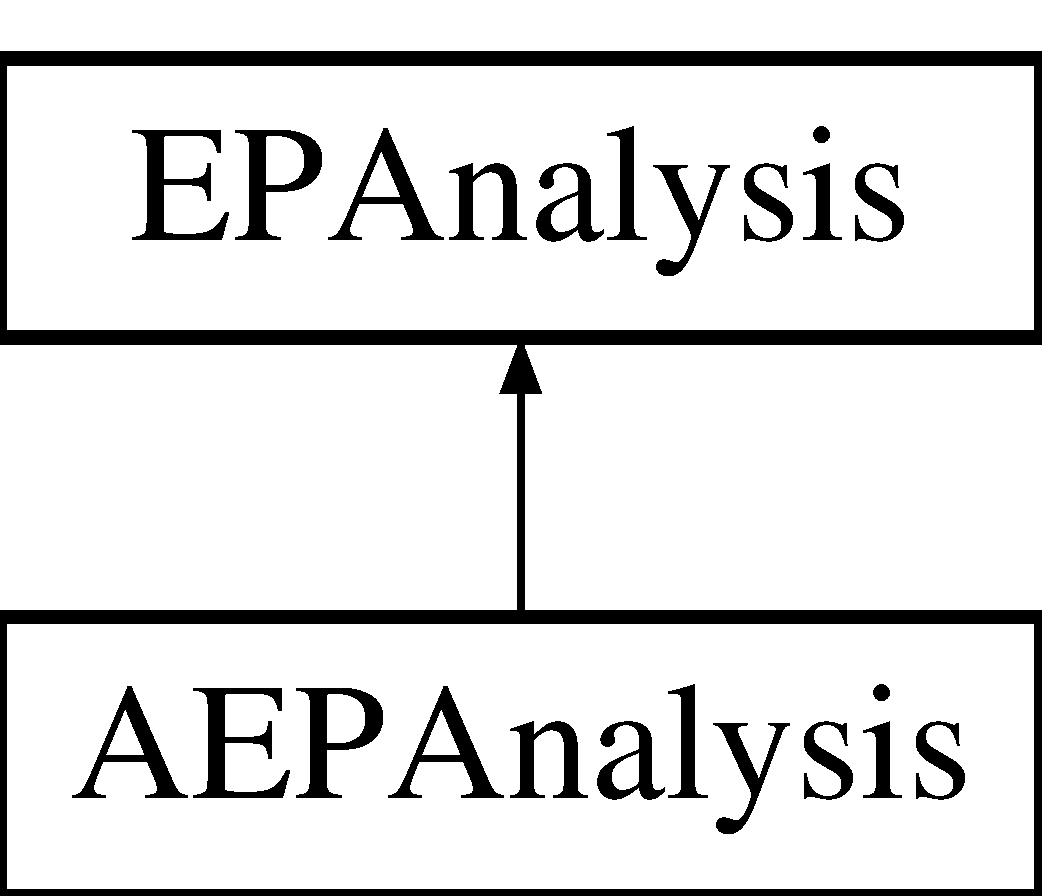
\includegraphics[height=2.000000cm]{class_a_e_p_analysis}
\end{center}
\end{figure}
\subsection*{Public Member Functions}
\begin{DoxyCompactItemize}
\item 
\hyperlink{class_a_e_p_analysis_abfb2164f3ed7f023c2172b9bcf8b1e23}{A\+E\+P\+Analysis} ()
\item 
\hyperlink{class_a_e_p_analysis_a9bed164d77fe6f0acfdc941b361ea56a}{$\sim$\+A\+E\+P\+Analysis} ()
\item 
virtual int \hyperlink{class_a_e_p_analysis_a6349405c9185f6ce4e4d3c5711daa217}{print\+Inf} (int from, int \hyperlink{lpc2spec_8m_a75a3ccc1a712583b6c4b21b94514a7b9}{end}=-\/1)
\item 
virtual void \hyperlink{class_a_e_p_analysis_af8c0797c01e6d50d4e3f5e89f98863a3}{Initial} (\hyperlink{class_raw_data}{Raw\+Data} $\ast$raw\+Data)
\item 
virtual void \hyperlink{class_a_e_p_analysis_abdec61d75b30f2d6753c3c237e2b6805}{calc\+One\+Block\+Background} (int index)
\item 
virtual void \hyperlink{class_a_e_p_analysis_a367b638a878435cf86de9b4b384b61a0}{calc\+One\+Block\+Speech} (int index)
\item 
virtual void \hyperlink{class_a_e_p_analysis_a270d364445bb9ed0d82f2bc15791c046}{calc\+One\+Block\+Other\+Data} (int index)
\end{DoxyCompactItemize}
\subsection*{Protected Member Functions}
\begin{DoxyCompactItemize}
\item 
virtual void \hyperlink{class_a_e_p_analysis_a4c230992b22dd17f64614148698a3a17}{save\+Other\+Data} (F\+I\+L\+E $\ast$\hyperlink{readhtk_8m_ae135fff58330ebb77574e0dd6280aa68}{fid})
\end{DoxyCompactItemize}
\subsection*{Protected Attributes}
\begin{DoxyCompactItemize}
\item 
vector$<$ double $>$ \hyperlink{class_a_e_p_analysis_a1a08690cf055caad8af6b95ce0e0f2c1}{level}
\end{DoxyCompactItemize}


\subsection{Constructor \& Destructor Documentation}
\hypertarget{class_a_e_p_analysis_abfb2164f3ed7f023c2172b9bcf8b1e23}{\index{A\+E\+P\+Analysis@{A\+E\+P\+Analysis}!A\+E\+P\+Analysis@{A\+E\+P\+Analysis}}
\index{A\+E\+P\+Analysis@{A\+E\+P\+Analysis}!A\+E\+P\+Analysis@{A\+E\+P\+Analysis}}
\subsubsection[{A\+E\+P\+Analysis}]{\setlength{\rightskip}{0pt plus 5cm}A\+E\+P\+Analysis\+::\+A\+E\+P\+Analysis (
\begin{DoxyParamCaption}
{}
\end{DoxyParamCaption}
)\hspace{0.3cm}{\ttfamily [inline]}}}\label{class_a_e_p_analysis_abfb2164f3ed7f023c2172b9bcf8b1e23}
\hypertarget{class_a_e_p_analysis_a9bed164d77fe6f0acfdc941b361ea56a}{\index{A\+E\+P\+Analysis@{A\+E\+P\+Analysis}!````~A\+E\+P\+Analysis@{$\sim$\+A\+E\+P\+Analysis}}
\index{````~A\+E\+P\+Analysis@{$\sim$\+A\+E\+P\+Analysis}!A\+E\+P\+Analysis@{A\+E\+P\+Analysis}}
\subsubsection[{$\sim$\+A\+E\+P\+Analysis}]{\setlength{\rightskip}{0pt plus 5cm}A\+E\+P\+Analysis\+::$\sim$\+A\+E\+P\+Analysis (
\begin{DoxyParamCaption}
{}
\end{DoxyParamCaption}
)\hspace{0.3cm}{\ttfamily [inline]}}}\label{class_a_e_p_analysis_a9bed164d77fe6f0acfdc941b361ea56a}


\subsection{Member Function Documentation}
\hypertarget{class_a_e_p_analysis_abdec61d75b30f2d6753c3c237e2b6805}{\index{A\+E\+P\+Analysis@{A\+E\+P\+Analysis}!calc\+One\+Block\+Background@{calc\+One\+Block\+Background}}
\index{calc\+One\+Block\+Background@{calc\+One\+Block\+Background}!A\+E\+P\+Analysis@{A\+E\+P\+Analysis}}
\subsubsection[{calc\+One\+Block\+Background}]{\setlength{\rightskip}{0pt plus 5cm}void A\+E\+P\+Analysis\+::calc\+One\+Block\+Background (
\begin{DoxyParamCaption}
\item[{int}]{index}
\end{DoxyParamCaption}
)\hspace{0.3cm}{\ttfamily [virtual]}}}\label{class_a_e_p_analysis_abdec61d75b30f2d6753c3c237e2b6805}


Implements \hyperlink{class_e_p_analysis_ac0d297dde8d0e9663f2e2e3b5fa0bc39}{E\+P\+Analysis}.

\hypertarget{class_a_e_p_analysis_a270d364445bb9ed0d82f2bc15791c046}{\index{A\+E\+P\+Analysis@{A\+E\+P\+Analysis}!calc\+One\+Block\+Other\+Data@{calc\+One\+Block\+Other\+Data}}
\index{calc\+One\+Block\+Other\+Data@{calc\+One\+Block\+Other\+Data}!A\+E\+P\+Analysis@{A\+E\+P\+Analysis}}
\subsubsection[{calc\+One\+Block\+Other\+Data}]{\setlength{\rightskip}{0pt plus 5cm}void A\+E\+P\+Analysis\+::calc\+One\+Block\+Other\+Data (
\begin{DoxyParamCaption}
\item[{int}]{index}
\end{DoxyParamCaption}
)\hspace{0.3cm}{\ttfamily [virtual]}}}\label{class_a_e_p_analysis_a270d364445bb9ed0d82f2bc15791c046}


Reimplemented from \hyperlink{class_e_p_analysis_aba99bc553c0e1f82ca844a5130263e6f}{E\+P\+Analysis}.

\hypertarget{class_a_e_p_analysis_a367b638a878435cf86de9b4b384b61a0}{\index{A\+E\+P\+Analysis@{A\+E\+P\+Analysis}!calc\+One\+Block\+Speech@{calc\+One\+Block\+Speech}}
\index{calc\+One\+Block\+Speech@{calc\+One\+Block\+Speech}!A\+E\+P\+Analysis@{A\+E\+P\+Analysis}}
\subsubsection[{calc\+One\+Block\+Speech}]{\setlength{\rightskip}{0pt plus 5cm}void A\+E\+P\+Analysis\+::calc\+One\+Block\+Speech (
\begin{DoxyParamCaption}
\item[{int}]{index}
\end{DoxyParamCaption}
)\hspace{0.3cm}{\ttfamily [virtual]}}}\label{class_a_e_p_analysis_a367b638a878435cf86de9b4b384b61a0}


Implements \hyperlink{class_e_p_analysis_a7767c0329b482231ec33faf935a620ce}{E\+P\+Analysis}.

\hypertarget{class_a_e_p_analysis_af8c0797c01e6d50d4e3f5e89f98863a3}{\index{A\+E\+P\+Analysis@{A\+E\+P\+Analysis}!Initial@{Initial}}
\index{Initial@{Initial}!A\+E\+P\+Analysis@{A\+E\+P\+Analysis}}
\subsubsection[{Initial}]{\setlength{\rightskip}{0pt plus 5cm}virtual void A\+E\+P\+Analysis\+::\+Initial (
\begin{DoxyParamCaption}
\item[{{\bf Raw\+Data} $\ast$}]{raw\+Data}
\end{DoxyParamCaption}
)\hspace{0.3cm}{\ttfamily [inline]}, {\ttfamily [virtual]}}}\label{class_a_e_p_analysis_af8c0797c01e6d50d4e3f5e89f98863a3}


Reimplemented from \hyperlink{class_e_p_analysis_a7e7311c513772986b89d97c7bde0eb39}{E\+P\+Analysis}.

\hypertarget{class_a_e_p_analysis_a6349405c9185f6ce4e4d3c5711daa217}{\index{A\+E\+P\+Analysis@{A\+E\+P\+Analysis}!print\+Inf@{print\+Inf}}
\index{print\+Inf@{print\+Inf}!A\+E\+P\+Analysis@{A\+E\+P\+Analysis}}
\subsubsection[{print\+Inf}]{\setlength{\rightskip}{0pt plus 5cm}int A\+E\+P\+Analysis\+::print\+Inf (
\begin{DoxyParamCaption}
\item[{int}]{from, }
\item[{int}]{end = {\ttfamily -\/1}}
\end{DoxyParamCaption}
)\hspace{0.3cm}{\ttfamily [virtual]}}}\label{class_a_e_p_analysis_a6349405c9185f6ce4e4d3c5711daa217}


Reimplemented from \hyperlink{class_e_p_analysis_a04fb7764261d7d579aa5bc98331b8a16}{E\+P\+Analysis}.

\hypertarget{class_a_e_p_analysis_a4c230992b22dd17f64614148698a3a17}{\index{A\+E\+P\+Analysis@{A\+E\+P\+Analysis}!save\+Other\+Data@{save\+Other\+Data}}
\index{save\+Other\+Data@{save\+Other\+Data}!A\+E\+P\+Analysis@{A\+E\+P\+Analysis}}
\subsubsection[{save\+Other\+Data}]{\setlength{\rightskip}{0pt plus 5cm}void A\+E\+P\+Analysis\+::save\+Other\+Data (
\begin{DoxyParamCaption}
\item[{F\+I\+L\+E $\ast$}]{fid}
\end{DoxyParamCaption}
)\hspace{0.3cm}{\ttfamily [protected]}, {\ttfamily [virtual]}}}\label{class_a_e_p_analysis_a4c230992b22dd17f64614148698a3a17}


Reimplemented from \hyperlink{class_e_p_analysis_a0c4270a435264c7aa18408d7f350ca31}{E\+P\+Analysis}.



\subsection{Member Data Documentation}
\hypertarget{class_a_e_p_analysis_a1a08690cf055caad8af6b95ce0e0f2c1}{\index{A\+E\+P\+Analysis@{A\+E\+P\+Analysis}!level@{level}}
\index{level@{level}!A\+E\+P\+Analysis@{A\+E\+P\+Analysis}}
\subsubsection[{level}]{\setlength{\rightskip}{0pt plus 5cm}vector$<$double$>$ A\+E\+P\+Analysis\+::level\hspace{0.3cm}{\ttfamily [protected]}}}\label{class_a_e_p_analysis_a1a08690cf055caad8af6b95ce0e0f2c1}


The documentation for this class was generated from the following files\+:\begin{DoxyCompactItemize}
\item 
src/\+Analysis/\hyperlink{_a_e_p_analysis_8h}{A\+E\+P\+Analysis.\+h}\item 
src/\+Analysis/\hyperlink{_a_e_p_analysis_8cpp}{A\+E\+P\+Analysis.\+cpp}\end{DoxyCompactItemize}

\hypertarget{class_a_p_p}{\section{A\+P\+P Class Reference}
\label{class_a_p_p}\index{A\+P\+P@{A\+P\+P}}
}


{\ttfamily \#include $<$app.\+h$>$}

\subsection*{Public Member Functions}
\begin{DoxyCompactItemize}
\item 
\hyperlink{class_a_p_p_a28503067508a0f6f6ddc78ac9e7ab3be}{A\+P\+P} ()
\item 
\hyperlink{class_a_p_p_a010865a1cf16fe5e9a9a565ae400e96e}{$\sim$\+A\+P\+P} ()
\item 
bool \hyperlink{class_a_p_p_a2027df94e77a9d42c81819e6fa693a43}{set\+Mode} (int \hyperlink{readhtk_8m_aaccc9105df5383111407fd5b41255e23}{t})
\item 
bool \hyperlink{class_a_p_p_a9ac588b2496c4d6e88a194d386218666}{set\+Alg} (int \hyperlink{readhtk_8m_aaccc9105df5383111407fd5b41255e23}{t})
\item 
bool \hyperlink{class_a_p_p_a7213f7a77a05f1a03d5cd3e69ef3ed83}{run} ()
\item 
\hyperlink{class_a_p_p_a28503067508a0f6f6ddc78ac9e7ab3be}{A\+P\+P} ()
\item 
\hyperlink{class_a_p_p_a010865a1cf16fe5e9a9a565ae400e96e}{$\sim$\+A\+P\+P} ()
\item 
bool \hyperlink{class_a_p_p_a2027df94e77a9d42c81819e6fa693a43}{set\+Mode} (int \hyperlink{readhtk_8m_aaccc9105df5383111407fd5b41255e23}{t})
\item 
bool \hyperlink{class_a_p_p_a9ac588b2496c4d6e88a194d386218666}{set\+Alg} (int \hyperlink{readhtk_8m_aaccc9105df5383111407fd5b41255e23}{t})
\item 
bool \hyperlink{class_a_p_p_a7213f7a77a05f1a03d5cd3e69ef3ed83}{run} ()
\end{DoxyCompactItemize}
\subsection*{Protected Member Functions}
\begin{DoxyCompactItemize}
\item 
\hyperlink{class_a_p_p_a6395700a096545c9cb93ed220324efee}{W\+R\+I\+T\+E\+\_\+\+O\+N\+L\+Y\+\_\+\+D\+E\+C\+L\+A\+R\+E} (char $\ast$, dict\+File, Dict)
\item 
\hyperlink{class_a_p_p_af01ec83f01316bfff6a546ea193bd78d}{W\+R\+I\+T\+E\+\_\+\+O\+N\+L\+Y\+\_\+\+D\+E\+C\+L\+A\+R\+E} (char $\ast$, better\+Story\+File, B\+Story)
\item 
\hyperlink{class_a_p_p_adf8e3638cc483b9f8835f22c3cefa1d8}{W\+R\+I\+T\+E\+\_\+\+O\+N\+L\+Y\+\_\+\+D\+E\+C\+L\+A\+R\+E} (char $\ast$, story\+File, Story)
\item 
\hyperlink{class_a_p_p_a3f492a4caa57a2cb5d2d8ef4b2171a26}{W\+R\+I\+T\+E\+\_\+\+O\+N\+L\+Y\+\_\+\+D\+E\+C\+L\+A\+R\+E} (char $\ast$, c\+Story\+File, C\+Story)
\item 
void \hyperlink{class_a_p_p_a329336a84831c48108262bd320944871}{calc\+Index} (const vector$<$ string $>$ \&org, vector$<$ int $>$ \&index)
\item 
bool \hyperlink{class_a_p_p_ab13dec33bbb35a260982031798af0566}{from\+File\+Job} ()
\item 
int \hyperlink{class_a_p_p_a2dfbe5c80d4997895be73f5134b1806e}{calc\+All\+With\+Thread} ()
\item 
int \hyperlink{class_a_p_p_adf4d3aa3c292a553ba12ad4d4adb8ed8}{calc\+One} ()
\item 
int \hyperlink{class_a_p_p_a6d7ca0077e251d59d0abba39ccfacd0a}{calc\+One\+With\+Dic} ()
\item 
bool \hyperlink{class_a_p_p_abe394dad8124de2b16ca6fa15fc1031f}{input\+Job} ()
\item 
void \hyperlink{class_a_p_p_a28855295319df5522e17b396e98a0134}{read\+File} ()
\item 
void \hyperlink{class_a_p_p_a7d0e3d031b5842c00910a734da39d027}{print\+Info} ()
\item 
void \hyperlink{class_a_p_p_aef7c54038f2695d4993d2f43ae535f1e}{print} (const vector$<$ string $>$ \&v, bool line=true) const 
\item 
void \hyperlink{class_a_p_p_a79b3882decc18c22c53d7bf9c1738201}{print} (const vector$<$ int $>$ \&index, const vector$<$ string $>$ \&v, bool line=true) const 
\item 
\hyperlink{class_a_p_p_a6395700a096545c9cb93ed220324efee}{W\+R\+I\+T\+E\+\_\+\+O\+N\+L\+Y\+\_\+\+D\+E\+C\+L\+A\+R\+E} (char $\ast$, dict\+File, Dict)
\item 
\hyperlink{class_a_p_p_af01ec83f01316bfff6a546ea193bd78d}{W\+R\+I\+T\+E\+\_\+\+O\+N\+L\+Y\+\_\+\+D\+E\+C\+L\+A\+R\+E} (char $\ast$, better\+Story\+File, B\+Story)
\item 
\hyperlink{class_a_p_p_adf8e3638cc483b9f8835f22c3cefa1d8}{W\+R\+I\+T\+E\+\_\+\+O\+N\+L\+Y\+\_\+\+D\+E\+C\+L\+A\+R\+E} (char $\ast$, story\+File, Story)
\item 
\hyperlink{class_a_p_p_a3f492a4caa57a2cb5d2d8ef4b2171a26}{W\+R\+I\+T\+E\+\_\+\+O\+N\+L\+Y\+\_\+\+D\+E\+C\+L\+A\+R\+E} (char $\ast$, c\+Story\+File, C\+Story)
\item 
void \hyperlink{class_a_p_p_a329336a84831c48108262bd320944871}{calc\+Index} (const vector$<$ string $>$ \&org, vector$<$ int $>$ \&index)
\item 
bool \hyperlink{class_a_p_p_ab13dec33bbb35a260982031798af0566}{from\+File\+Job} ()
\item 
int \hyperlink{class_a_p_p_a2dfbe5c80d4997895be73f5134b1806e}{calc\+All\+With\+Thread} ()
\item 
int \hyperlink{class_a_p_p_adf4d3aa3c292a553ba12ad4d4adb8ed8}{calc\+One} ()
\item 
int \hyperlink{class_a_p_p_a6d7ca0077e251d59d0abba39ccfacd0a}{calc\+One\+With\+Dic} ()
\item 
bool \hyperlink{class_a_p_p_abe394dad8124de2b16ca6fa15fc1031f}{input\+Job} ()
\item 
void \hyperlink{class_a_p_p_a28855295319df5522e17b396e98a0134}{read\+File} ()
\item 
void \hyperlink{class_a_p_p_a7d0e3d031b5842c00910a734da39d027}{print\+Info} ()
\item 
void \hyperlink{class_a_p_p_aef7c54038f2695d4993d2f43ae535f1e}{print} (const vector$<$ string $>$ \&v, bool line=true) const 
\item 
void \hyperlink{class_a_p_p_a79b3882decc18c22c53d7bf9c1738201}{print} (const vector$<$ int $>$ \&index, const vector$<$ string $>$ \&v, bool line=true) const 
\end{DoxyCompactItemize}
\subsection*{Static Protected Member Functions}
\begin{DoxyCompactItemize}
\item 
static void \hyperlink{class_a_p_p_a643d26fb5b685c7a1a9ca0f907722241}{cmp\+\_\+task} (void $\ast$in)
\item 
static void \hyperlink{class_a_p_p_abdbe780dfdb0886e27c6744df079f38a}{cmp\+\_\+task} (void $\ast$in)
\end{DoxyCompactItemize}
\subsection*{Protected Attributes}
\begin{DoxyCompactItemize}
\item 
vector$<$ string $>$ \hyperlink{class_a_p_p_ac5841d717fc07ad656b743f86336b8a5}{story}
\item 
vector$<$ string $>$ \hyperlink{class_a_p_p_a599d2539b3815e510bf1f1be28e4047f}{c\+Story}
\item 
vector$<$ \hyperlink{struct_path}{Path} $>$ \hyperlink{class_a_p_p_aa2aee15bbba3ab5ba5b6c9e120068a0e}{paths}
\item 
vector$<$ int $>$ \hyperlink{class_a_p_p_abe393707ad5d1aa537ddbb4428b84c32}{story\+Index}
\item 
vector$<$ string $>$ \hyperlink{class_a_p_p_ad434309fd56f06dace1a73e0a8b069d9}{dic}
\item 
vector$<$ int $>$ \hyperlink{class_a_p_p_a5ab0c5c949700e522f41ee4a8c35de52}{better}
\item 
int \hyperlink{class_a_p_p_a09ff32362a370e70a2b0c8dfc2f4b406}{alg}
\item 
int \hyperlink{class_a_p_p_a799513151a59f01ffcbbf5ba85a2d1c6}{mode}
\end{DoxyCompactItemize}
\subsection*{Private Member Functions}
\begin{DoxyCompactItemize}
\item 
\hyperlink{class_a_p_p_a93969636f8cee0d293fc8817843532f2}{W\+R\+I\+T\+E\+\_\+\+O\+N\+L\+Y\+\_\+\+D\+E\+C\+L\+A\+R\+E} (bool, from\+File, From\+File)
\item 
\hyperlink{class_a_p_p_a93969636f8cee0d293fc8817843532f2}{W\+R\+I\+T\+E\+\_\+\+O\+N\+L\+Y\+\_\+\+D\+E\+C\+L\+A\+R\+E} (bool, from\+File, From\+File)
\end{DoxyCompactItemize}


\subsection{Constructor \& Destructor Documentation}
\hypertarget{class_a_p_p_a28503067508a0f6f6ddc78ac9e7ab3be}{\index{A\+P\+P@{A\+P\+P}!A\+P\+P@{A\+P\+P}}
\index{A\+P\+P@{A\+P\+P}!A\+P\+P@{A\+P\+P}}
\subsubsection[{A\+P\+P}]{\setlength{\rightskip}{0pt plus 5cm}A\+P\+P\+::\+A\+P\+P (
\begin{DoxyParamCaption}
{}
\end{DoxyParamCaption}
)}}\label{class_a_p_p_a28503067508a0f6f6ddc78ac9e7ab3be}
\hypertarget{class_a_p_p_a010865a1cf16fe5e9a9a565ae400e96e}{\index{A\+P\+P@{A\+P\+P}!````~A\+P\+P@{$\sim$\+A\+P\+P}}
\index{````~A\+P\+P@{$\sim$\+A\+P\+P}!A\+P\+P@{A\+P\+P}}
\subsubsection[{$\sim$\+A\+P\+P}]{\setlength{\rightskip}{0pt plus 5cm}A\+P\+P\+::$\sim$\+A\+P\+P (
\begin{DoxyParamCaption}
{}
\end{DoxyParamCaption}
)}}\label{class_a_p_p_a010865a1cf16fe5e9a9a565ae400e96e}
\hypertarget{class_a_p_p_a28503067508a0f6f6ddc78ac9e7ab3be}{\index{A\+P\+P@{A\+P\+P}!A\+P\+P@{A\+P\+P}}
\index{A\+P\+P@{A\+P\+P}!A\+P\+P@{A\+P\+P}}
\subsubsection[{A\+P\+P}]{\setlength{\rightskip}{0pt plus 5cm}A\+P\+P\+::\+A\+P\+P (
\begin{DoxyParamCaption}
{}
\end{DoxyParamCaption}
)}}\label{class_a_p_p_a28503067508a0f6f6ddc78ac9e7ab3be}
\hypertarget{class_a_p_p_a010865a1cf16fe5e9a9a565ae400e96e}{\index{A\+P\+P@{A\+P\+P}!````~A\+P\+P@{$\sim$\+A\+P\+P}}
\index{````~A\+P\+P@{$\sim$\+A\+P\+P}!A\+P\+P@{A\+P\+P}}
\subsubsection[{$\sim$\+A\+P\+P}]{\setlength{\rightskip}{0pt plus 5cm}A\+P\+P\+::$\sim$\+A\+P\+P (
\begin{DoxyParamCaption}
{}
\end{DoxyParamCaption}
)}}\label{class_a_p_p_a010865a1cf16fe5e9a9a565ae400e96e}


\subsection{Member Function Documentation}
\hypertarget{class_a_p_p_a2dfbe5c80d4997895be73f5134b1806e}{\index{A\+P\+P@{A\+P\+P}!calc\+All\+With\+Thread@{calc\+All\+With\+Thread}}
\index{calc\+All\+With\+Thread@{calc\+All\+With\+Thread}!A\+P\+P@{A\+P\+P}}
\subsubsection[{calc\+All\+With\+Thread}]{\setlength{\rightskip}{0pt plus 5cm}int A\+P\+P\+::calc\+All\+With\+Thread (
\begin{DoxyParamCaption}
{}
\end{DoxyParamCaption}
)\hspace{0.3cm}{\ttfamily [protected]}}}\label{class_a_p_p_a2dfbe5c80d4997895be73f5134b1806e}
\hypertarget{class_a_p_p_a2dfbe5c80d4997895be73f5134b1806e}{\index{A\+P\+P@{A\+P\+P}!calc\+All\+With\+Thread@{calc\+All\+With\+Thread}}
\index{calc\+All\+With\+Thread@{calc\+All\+With\+Thread}!A\+P\+P@{A\+P\+P}}
\subsubsection[{calc\+All\+With\+Thread}]{\setlength{\rightskip}{0pt plus 5cm}int A\+P\+P\+::calc\+All\+With\+Thread (
\begin{DoxyParamCaption}
{}
\end{DoxyParamCaption}
)\hspace{0.3cm}{\ttfamily [protected]}}}\label{class_a_p_p_a2dfbe5c80d4997895be73f5134b1806e}
\hypertarget{class_a_p_p_a329336a84831c48108262bd320944871}{\index{A\+P\+P@{A\+P\+P}!calc\+Index@{calc\+Index}}
\index{calc\+Index@{calc\+Index}!A\+P\+P@{A\+P\+P}}
\subsubsection[{calc\+Index}]{\setlength{\rightskip}{0pt plus 5cm}void A\+P\+P\+::calc\+Index (
\begin{DoxyParamCaption}
\item[{const vector$<$ string $>$ \&}]{org, }
\item[{vector$<$ int $>$ \&}]{index}
\end{DoxyParamCaption}
)\hspace{0.3cm}{\ttfamily [protected]}}}\label{class_a_p_p_a329336a84831c48108262bd320944871}
\hypertarget{class_a_p_p_a329336a84831c48108262bd320944871}{\index{A\+P\+P@{A\+P\+P}!calc\+Index@{calc\+Index}}
\index{calc\+Index@{calc\+Index}!A\+P\+P@{A\+P\+P}}
\subsubsection[{calc\+Index}]{\setlength{\rightskip}{0pt plus 5cm}void A\+P\+P\+::calc\+Index (
\begin{DoxyParamCaption}
\item[{const vector$<$ string $>$ \&}]{org, }
\item[{vector$<$ int $>$ \&}]{index}
\end{DoxyParamCaption}
)\hspace{0.3cm}{\ttfamily [protected]}}}\label{class_a_p_p_a329336a84831c48108262bd320944871}
\hypertarget{class_a_p_p_adf4d3aa3c292a553ba12ad4d4adb8ed8}{\index{A\+P\+P@{A\+P\+P}!calc\+One@{calc\+One}}
\index{calc\+One@{calc\+One}!A\+P\+P@{A\+P\+P}}
\subsubsection[{calc\+One}]{\setlength{\rightskip}{0pt plus 5cm}int A\+P\+P\+::calc\+One (
\begin{DoxyParamCaption}
{}
\end{DoxyParamCaption}
)\hspace{0.3cm}{\ttfamily [protected]}}}\label{class_a_p_p_adf4d3aa3c292a553ba12ad4d4adb8ed8}
\hypertarget{class_a_p_p_adf4d3aa3c292a553ba12ad4d4adb8ed8}{\index{A\+P\+P@{A\+P\+P}!calc\+One@{calc\+One}}
\index{calc\+One@{calc\+One}!A\+P\+P@{A\+P\+P}}
\subsubsection[{calc\+One}]{\setlength{\rightskip}{0pt plus 5cm}int A\+P\+P\+::calc\+One (
\begin{DoxyParamCaption}
{}
\end{DoxyParamCaption}
)\hspace{0.3cm}{\ttfamily [protected]}}}\label{class_a_p_p_adf4d3aa3c292a553ba12ad4d4adb8ed8}
\hypertarget{class_a_p_p_a6d7ca0077e251d59d0abba39ccfacd0a}{\index{A\+P\+P@{A\+P\+P}!calc\+One\+With\+Dic@{calc\+One\+With\+Dic}}
\index{calc\+One\+With\+Dic@{calc\+One\+With\+Dic}!A\+P\+P@{A\+P\+P}}
\subsubsection[{calc\+One\+With\+Dic}]{\setlength{\rightskip}{0pt plus 5cm}int A\+P\+P\+::calc\+One\+With\+Dic (
\begin{DoxyParamCaption}
{}
\end{DoxyParamCaption}
)\hspace{0.3cm}{\ttfamily [protected]}}}\label{class_a_p_p_a6d7ca0077e251d59d0abba39ccfacd0a}
\hypertarget{class_a_p_p_a6d7ca0077e251d59d0abba39ccfacd0a}{\index{A\+P\+P@{A\+P\+P}!calc\+One\+With\+Dic@{calc\+One\+With\+Dic}}
\index{calc\+One\+With\+Dic@{calc\+One\+With\+Dic}!A\+P\+P@{A\+P\+P}}
\subsubsection[{calc\+One\+With\+Dic}]{\setlength{\rightskip}{0pt plus 5cm}int A\+P\+P\+::calc\+One\+With\+Dic (
\begin{DoxyParamCaption}
{}
\end{DoxyParamCaption}
)\hspace{0.3cm}{\ttfamily [protected]}}}\label{class_a_p_p_a6d7ca0077e251d59d0abba39ccfacd0a}
\hypertarget{class_a_p_p_abdbe780dfdb0886e27c6744df079f38a}{\index{A\+P\+P@{A\+P\+P}!cmp\+\_\+task@{cmp\+\_\+task}}
\index{cmp\+\_\+task@{cmp\+\_\+task}!A\+P\+P@{A\+P\+P}}
\subsubsection[{cmp\+\_\+task}]{\setlength{\rightskip}{0pt plus 5cm}static void A\+P\+P\+::cmp\+\_\+task (
\begin{DoxyParamCaption}
\item[{void $\ast$}]{in}
\end{DoxyParamCaption}
)\hspace{0.3cm}{\ttfamily [static]}, {\ttfamily [protected]}}}\label{class_a_p_p_abdbe780dfdb0886e27c6744df079f38a}
\hypertarget{class_a_p_p_a643d26fb5b685c7a1a9ca0f907722241}{\index{A\+P\+P@{A\+P\+P}!cmp\+\_\+task@{cmp\+\_\+task}}
\index{cmp\+\_\+task@{cmp\+\_\+task}!A\+P\+P@{A\+P\+P}}
\subsubsection[{cmp\+\_\+task}]{\setlength{\rightskip}{0pt plus 5cm}void A\+P\+P\+::cmp\+\_\+task (
\begin{DoxyParamCaption}
\item[{void $\ast$}]{in}
\end{DoxyParamCaption}
)\hspace{0.3cm}{\ttfamily [static]}, {\ttfamily [protected]}}}\label{class_a_p_p_a643d26fb5b685c7a1a9ca0f907722241}
\hypertarget{class_a_p_p_ab13dec33bbb35a260982031798af0566}{\index{A\+P\+P@{A\+P\+P}!from\+File\+Job@{from\+File\+Job}}
\index{from\+File\+Job@{from\+File\+Job}!A\+P\+P@{A\+P\+P}}
\subsubsection[{from\+File\+Job}]{\setlength{\rightskip}{0pt plus 5cm}bool A\+P\+P\+::from\+File\+Job (
\begin{DoxyParamCaption}
{}
\end{DoxyParamCaption}
)\hspace{0.3cm}{\ttfamily [protected]}}}\label{class_a_p_p_ab13dec33bbb35a260982031798af0566}
\hypertarget{class_a_p_p_ab13dec33bbb35a260982031798af0566}{\index{A\+P\+P@{A\+P\+P}!from\+File\+Job@{from\+File\+Job}}
\index{from\+File\+Job@{from\+File\+Job}!A\+P\+P@{A\+P\+P}}
\subsubsection[{from\+File\+Job}]{\setlength{\rightskip}{0pt plus 5cm}bool A\+P\+P\+::from\+File\+Job (
\begin{DoxyParamCaption}
{}
\end{DoxyParamCaption}
)\hspace{0.3cm}{\ttfamily [protected]}}}\label{class_a_p_p_ab13dec33bbb35a260982031798af0566}
\hypertarget{class_a_p_p_abe394dad8124de2b16ca6fa15fc1031f}{\index{A\+P\+P@{A\+P\+P}!input\+Job@{input\+Job}}
\index{input\+Job@{input\+Job}!A\+P\+P@{A\+P\+P}}
\subsubsection[{input\+Job}]{\setlength{\rightskip}{0pt plus 5cm}bool A\+P\+P\+::input\+Job (
\begin{DoxyParamCaption}
{}
\end{DoxyParamCaption}
)\hspace{0.3cm}{\ttfamily [protected]}}}\label{class_a_p_p_abe394dad8124de2b16ca6fa15fc1031f}
\hypertarget{class_a_p_p_abe394dad8124de2b16ca6fa15fc1031f}{\index{A\+P\+P@{A\+P\+P}!input\+Job@{input\+Job}}
\index{input\+Job@{input\+Job}!A\+P\+P@{A\+P\+P}}
\subsubsection[{input\+Job}]{\setlength{\rightskip}{0pt plus 5cm}bool A\+P\+P\+::input\+Job (
\begin{DoxyParamCaption}
{}
\end{DoxyParamCaption}
)\hspace{0.3cm}{\ttfamily [protected]}}}\label{class_a_p_p_abe394dad8124de2b16ca6fa15fc1031f}
\hypertarget{class_a_p_p_aef7c54038f2695d4993d2f43ae535f1e}{\index{A\+P\+P@{A\+P\+P}!print@{print}}
\index{print@{print}!A\+P\+P@{A\+P\+P}}
\subsubsection[{print}]{\setlength{\rightskip}{0pt plus 5cm}void A\+P\+P\+::print (
\begin{DoxyParamCaption}
\item[{const vector$<$ string $>$ \&}]{v, }
\item[{bool}]{line = {\ttfamily true}}
\end{DoxyParamCaption}
) const\hspace{0.3cm}{\ttfamily [protected]}}}\label{class_a_p_p_aef7c54038f2695d4993d2f43ae535f1e}
\hypertarget{class_a_p_p_a79b3882decc18c22c53d7bf9c1738201}{\index{A\+P\+P@{A\+P\+P}!print@{print}}
\index{print@{print}!A\+P\+P@{A\+P\+P}}
\subsubsection[{print}]{\setlength{\rightskip}{0pt plus 5cm}void A\+P\+P\+::print (
\begin{DoxyParamCaption}
\item[{const vector$<$ int $>$ \&}]{index, }
\item[{const vector$<$ string $>$ \&}]{v, }
\item[{bool}]{line = {\ttfamily true}}
\end{DoxyParamCaption}
) const\hspace{0.3cm}{\ttfamily [protected]}}}\label{class_a_p_p_a79b3882decc18c22c53d7bf9c1738201}
\hypertarget{class_a_p_p_aef7c54038f2695d4993d2f43ae535f1e}{\index{A\+P\+P@{A\+P\+P}!print@{print}}
\index{print@{print}!A\+P\+P@{A\+P\+P}}
\subsubsection[{print}]{\setlength{\rightskip}{0pt plus 5cm}void A\+P\+P\+::print (
\begin{DoxyParamCaption}
\item[{const vector$<$ string $>$ \&}]{v, }
\item[{bool}]{line = {\ttfamily true}}
\end{DoxyParamCaption}
) const\hspace{0.3cm}{\ttfamily [protected]}}}\label{class_a_p_p_aef7c54038f2695d4993d2f43ae535f1e}
\hypertarget{class_a_p_p_a79b3882decc18c22c53d7bf9c1738201}{\index{A\+P\+P@{A\+P\+P}!print@{print}}
\index{print@{print}!A\+P\+P@{A\+P\+P}}
\subsubsection[{print}]{\setlength{\rightskip}{0pt plus 5cm}void A\+P\+P\+::print (
\begin{DoxyParamCaption}
\item[{const vector$<$ int $>$ \&}]{index, }
\item[{const vector$<$ string $>$ \&}]{v, }
\item[{bool}]{line = {\ttfamily true}}
\end{DoxyParamCaption}
) const\hspace{0.3cm}{\ttfamily [protected]}}}\label{class_a_p_p_a79b3882decc18c22c53d7bf9c1738201}
\hypertarget{class_a_p_p_a7d0e3d031b5842c00910a734da39d027}{\index{A\+P\+P@{A\+P\+P}!print\+Info@{print\+Info}}
\index{print\+Info@{print\+Info}!A\+P\+P@{A\+P\+P}}
\subsubsection[{print\+Info}]{\setlength{\rightskip}{0pt plus 5cm}void A\+P\+P\+::print\+Info (
\begin{DoxyParamCaption}
{}
\end{DoxyParamCaption}
)\hspace{0.3cm}{\ttfamily [protected]}}}\label{class_a_p_p_a7d0e3d031b5842c00910a734da39d027}
\hypertarget{class_a_p_p_a7d0e3d031b5842c00910a734da39d027}{\index{A\+P\+P@{A\+P\+P}!print\+Info@{print\+Info}}
\index{print\+Info@{print\+Info}!A\+P\+P@{A\+P\+P}}
\subsubsection[{print\+Info}]{\setlength{\rightskip}{0pt plus 5cm}void A\+P\+P\+::print\+Info (
\begin{DoxyParamCaption}
{}
\end{DoxyParamCaption}
)\hspace{0.3cm}{\ttfamily [protected]}}}\label{class_a_p_p_a7d0e3d031b5842c00910a734da39d027}
\hypertarget{class_a_p_p_a28855295319df5522e17b396e98a0134}{\index{A\+P\+P@{A\+P\+P}!read\+File@{read\+File}}
\index{read\+File@{read\+File}!A\+P\+P@{A\+P\+P}}
\subsubsection[{read\+File}]{\setlength{\rightskip}{0pt plus 5cm}void A\+P\+P\+::read\+File (
\begin{DoxyParamCaption}
{}
\end{DoxyParamCaption}
)\hspace{0.3cm}{\ttfamily [protected]}}}\label{class_a_p_p_a28855295319df5522e17b396e98a0134}
\hypertarget{class_a_p_p_a28855295319df5522e17b396e98a0134}{\index{A\+P\+P@{A\+P\+P}!read\+File@{read\+File}}
\index{read\+File@{read\+File}!A\+P\+P@{A\+P\+P}}
\subsubsection[{read\+File}]{\setlength{\rightskip}{0pt plus 5cm}void A\+P\+P\+::read\+File (
\begin{DoxyParamCaption}
{}
\end{DoxyParamCaption}
)\hspace{0.3cm}{\ttfamily [protected]}}}\label{class_a_p_p_a28855295319df5522e17b396e98a0134}
\hypertarget{class_a_p_p_a7213f7a77a05f1a03d5cd3e69ef3ed83}{\index{A\+P\+P@{A\+P\+P}!run@{run}}
\index{run@{run}!A\+P\+P@{A\+P\+P}}
\subsubsection[{run}]{\setlength{\rightskip}{0pt plus 5cm}bool A\+P\+P\+::run (
\begin{DoxyParamCaption}
{}
\end{DoxyParamCaption}
)}}\label{class_a_p_p_a7213f7a77a05f1a03d5cd3e69ef3ed83}
\hypertarget{class_a_p_p_a7213f7a77a05f1a03d5cd3e69ef3ed83}{\index{A\+P\+P@{A\+P\+P}!run@{run}}
\index{run@{run}!A\+P\+P@{A\+P\+P}}
\subsubsection[{run}]{\setlength{\rightskip}{0pt plus 5cm}bool A\+P\+P\+::run (
\begin{DoxyParamCaption}
{}
\end{DoxyParamCaption}
)}}\label{class_a_p_p_a7213f7a77a05f1a03d5cd3e69ef3ed83}
\hypertarget{class_a_p_p_a9ac588b2496c4d6e88a194d386218666}{\index{A\+P\+P@{A\+P\+P}!set\+Alg@{set\+Alg}}
\index{set\+Alg@{set\+Alg}!A\+P\+P@{A\+P\+P}}
\subsubsection[{set\+Alg}]{\setlength{\rightskip}{0pt plus 5cm}bool A\+P\+P\+::set\+Alg (
\begin{DoxyParamCaption}
\item[{int}]{t}
\end{DoxyParamCaption}
)}}\label{class_a_p_p_a9ac588b2496c4d6e88a194d386218666}
\hypertarget{class_a_p_p_a9ac588b2496c4d6e88a194d386218666}{\index{A\+P\+P@{A\+P\+P}!set\+Alg@{set\+Alg}}
\index{set\+Alg@{set\+Alg}!A\+P\+P@{A\+P\+P}}
\subsubsection[{set\+Alg}]{\setlength{\rightskip}{0pt plus 5cm}bool A\+P\+P\+::set\+Alg (
\begin{DoxyParamCaption}
\item[{int}]{t}
\end{DoxyParamCaption}
)}}\label{class_a_p_p_a9ac588b2496c4d6e88a194d386218666}
\hypertarget{class_a_p_p_a2027df94e77a9d42c81819e6fa693a43}{\index{A\+P\+P@{A\+P\+P}!set\+Mode@{set\+Mode}}
\index{set\+Mode@{set\+Mode}!A\+P\+P@{A\+P\+P}}
\subsubsection[{set\+Mode}]{\setlength{\rightskip}{0pt plus 5cm}bool A\+P\+P\+::set\+Mode (
\begin{DoxyParamCaption}
\item[{int}]{t}
\end{DoxyParamCaption}
)}}\label{class_a_p_p_a2027df94e77a9d42c81819e6fa693a43}
\hypertarget{class_a_p_p_a2027df94e77a9d42c81819e6fa693a43}{\index{A\+P\+P@{A\+P\+P}!set\+Mode@{set\+Mode}}
\index{set\+Mode@{set\+Mode}!A\+P\+P@{A\+P\+P}}
\subsubsection[{set\+Mode}]{\setlength{\rightskip}{0pt plus 5cm}bool A\+P\+P\+::set\+Mode (
\begin{DoxyParamCaption}
\item[{int}]{t}
\end{DoxyParamCaption}
)}}\label{class_a_p_p_a2027df94e77a9d42c81819e6fa693a43}
\hypertarget{class_a_p_p_a93969636f8cee0d293fc8817843532f2}{\index{A\+P\+P@{A\+P\+P}!W\+R\+I\+T\+E\+\_\+\+O\+N\+L\+Y\+\_\+\+D\+E\+C\+L\+A\+R\+E@{W\+R\+I\+T\+E\+\_\+\+O\+N\+L\+Y\+\_\+\+D\+E\+C\+L\+A\+R\+E}}
\index{W\+R\+I\+T\+E\+\_\+\+O\+N\+L\+Y\+\_\+\+D\+E\+C\+L\+A\+R\+E@{W\+R\+I\+T\+E\+\_\+\+O\+N\+L\+Y\+\_\+\+D\+E\+C\+L\+A\+R\+E}!A\+P\+P@{A\+P\+P}}
\subsubsection[{W\+R\+I\+T\+E\+\_\+\+O\+N\+L\+Y\+\_\+\+D\+E\+C\+L\+A\+R\+E}]{\setlength{\rightskip}{0pt plus 5cm}A\+P\+P\+::\+W\+R\+I\+T\+E\+\_\+\+O\+N\+L\+Y\+\_\+\+D\+E\+C\+L\+A\+R\+E (
\begin{DoxyParamCaption}
\item[{bool}]{, }
\item[{from\+File}]{, }
\item[{From\+File}]{}
\end{DoxyParamCaption}
)\hspace{0.3cm}{\ttfamily [private]}}}\label{class_a_p_p_a93969636f8cee0d293fc8817843532f2}
\hypertarget{class_a_p_p_a93969636f8cee0d293fc8817843532f2}{\index{A\+P\+P@{A\+P\+P}!W\+R\+I\+T\+E\+\_\+\+O\+N\+L\+Y\+\_\+\+D\+E\+C\+L\+A\+R\+E@{W\+R\+I\+T\+E\+\_\+\+O\+N\+L\+Y\+\_\+\+D\+E\+C\+L\+A\+R\+E}}
\index{W\+R\+I\+T\+E\+\_\+\+O\+N\+L\+Y\+\_\+\+D\+E\+C\+L\+A\+R\+E@{W\+R\+I\+T\+E\+\_\+\+O\+N\+L\+Y\+\_\+\+D\+E\+C\+L\+A\+R\+E}!A\+P\+P@{A\+P\+P}}
\subsubsection[{W\+R\+I\+T\+E\+\_\+\+O\+N\+L\+Y\+\_\+\+D\+E\+C\+L\+A\+R\+E}]{\setlength{\rightskip}{0pt plus 5cm}A\+P\+P\+::\+W\+R\+I\+T\+E\+\_\+\+O\+N\+L\+Y\+\_\+\+D\+E\+C\+L\+A\+R\+E (
\begin{DoxyParamCaption}
\item[{bool}]{, }
\item[{from\+File}]{, }
\item[{From\+File}]{}
\end{DoxyParamCaption}
)\hspace{0.3cm}{\ttfamily [private]}}}\label{class_a_p_p_a93969636f8cee0d293fc8817843532f2}
\hypertarget{class_a_p_p_a6395700a096545c9cb93ed220324efee}{\index{A\+P\+P@{A\+P\+P}!W\+R\+I\+T\+E\+\_\+\+O\+N\+L\+Y\+\_\+\+D\+E\+C\+L\+A\+R\+E@{W\+R\+I\+T\+E\+\_\+\+O\+N\+L\+Y\+\_\+\+D\+E\+C\+L\+A\+R\+E}}
\index{W\+R\+I\+T\+E\+\_\+\+O\+N\+L\+Y\+\_\+\+D\+E\+C\+L\+A\+R\+E@{W\+R\+I\+T\+E\+\_\+\+O\+N\+L\+Y\+\_\+\+D\+E\+C\+L\+A\+R\+E}!A\+P\+P@{A\+P\+P}}
\subsubsection[{W\+R\+I\+T\+E\+\_\+\+O\+N\+L\+Y\+\_\+\+D\+E\+C\+L\+A\+R\+E}]{\setlength{\rightskip}{0pt plus 5cm}A\+P\+P\+::\+W\+R\+I\+T\+E\+\_\+\+O\+N\+L\+Y\+\_\+\+D\+E\+C\+L\+A\+R\+E (
\begin{DoxyParamCaption}
\item[{char $\ast$}]{, }
\item[{dict\+File}]{, }
\item[{Dict}]{}
\end{DoxyParamCaption}
)\hspace{0.3cm}{\ttfamily [protected]}}}\label{class_a_p_p_a6395700a096545c9cb93ed220324efee}
\hypertarget{class_a_p_p_a6395700a096545c9cb93ed220324efee}{\index{A\+P\+P@{A\+P\+P}!W\+R\+I\+T\+E\+\_\+\+O\+N\+L\+Y\+\_\+\+D\+E\+C\+L\+A\+R\+E@{W\+R\+I\+T\+E\+\_\+\+O\+N\+L\+Y\+\_\+\+D\+E\+C\+L\+A\+R\+E}}
\index{W\+R\+I\+T\+E\+\_\+\+O\+N\+L\+Y\+\_\+\+D\+E\+C\+L\+A\+R\+E@{W\+R\+I\+T\+E\+\_\+\+O\+N\+L\+Y\+\_\+\+D\+E\+C\+L\+A\+R\+E}!A\+P\+P@{A\+P\+P}}
\subsubsection[{W\+R\+I\+T\+E\+\_\+\+O\+N\+L\+Y\+\_\+\+D\+E\+C\+L\+A\+R\+E}]{\setlength{\rightskip}{0pt plus 5cm}A\+P\+P\+::\+W\+R\+I\+T\+E\+\_\+\+O\+N\+L\+Y\+\_\+\+D\+E\+C\+L\+A\+R\+E (
\begin{DoxyParamCaption}
\item[{char $\ast$}]{, }
\item[{dict\+File}]{, }
\item[{Dict}]{}
\end{DoxyParamCaption}
)\hspace{0.3cm}{\ttfamily [protected]}}}\label{class_a_p_p_a6395700a096545c9cb93ed220324efee}
\hypertarget{class_a_p_p_af01ec83f01316bfff6a546ea193bd78d}{\index{A\+P\+P@{A\+P\+P}!W\+R\+I\+T\+E\+\_\+\+O\+N\+L\+Y\+\_\+\+D\+E\+C\+L\+A\+R\+E@{W\+R\+I\+T\+E\+\_\+\+O\+N\+L\+Y\+\_\+\+D\+E\+C\+L\+A\+R\+E}}
\index{W\+R\+I\+T\+E\+\_\+\+O\+N\+L\+Y\+\_\+\+D\+E\+C\+L\+A\+R\+E@{W\+R\+I\+T\+E\+\_\+\+O\+N\+L\+Y\+\_\+\+D\+E\+C\+L\+A\+R\+E}!A\+P\+P@{A\+P\+P}}
\subsubsection[{W\+R\+I\+T\+E\+\_\+\+O\+N\+L\+Y\+\_\+\+D\+E\+C\+L\+A\+R\+E}]{\setlength{\rightskip}{0pt plus 5cm}A\+P\+P\+::\+W\+R\+I\+T\+E\+\_\+\+O\+N\+L\+Y\+\_\+\+D\+E\+C\+L\+A\+R\+E (
\begin{DoxyParamCaption}
\item[{char $\ast$}]{, }
\item[{better\+Story\+File}]{, }
\item[{B\+Story}]{}
\end{DoxyParamCaption}
)\hspace{0.3cm}{\ttfamily [protected]}}}\label{class_a_p_p_af01ec83f01316bfff6a546ea193bd78d}
\hypertarget{class_a_p_p_af01ec83f01316bfff6a546ea193bd78d}{\index{A\+P\+P@{A\+P\+P}!W\+R\+I\+T\+E\+\_\+\+O\+N\+L\+Y\+\_\+\+D\+E\+C\+L\+A\+R\+E@{W\+R\+I\+T\+E\+\_\+\+O\+N\+L\+Y\+\_\+\+D\+E\+C\+L\+A\+R\+E}}
\index{W\+R\+I\+T\+E\+\_\+\+O\+N\+L\+Y\+\_\+\+D\+E\+C\+L\+A\+R\+E@{W\+R\+I\+T\+E\+\_\+\+O\+N\+L\+Y\+\_\+\+D\+E\+C\+L\+A\+R\+E}!A\+P\+P@{A\+P\+P}}
\subsubsection[{W\+R\+I\+T\+E\+\_\+\+O\+N\+L\+Y\+\_\+\+D\+E\+C\+L\+A\+R\+E}]{\setlength{\rightskip}{0pt plus 5cm}A\+P\+P\+::\+W\+R\+I\+T\+E\+\_\+\+O\+N\+L\+Y\+\_\+\+D\+E\+C\+L\+A\+R\+E (
\begin{DoxyParamCaption}
\item[{char $\ast$}]{, }
\item[{better\+Story\+File}]{, }
\item[{B\+Story}]{}
\end{DoxyParamCaption}
)\hspace{0.3cm}{\ttfamily [protected]}}}\label{class_a_p_p_af01ec83f01316bfff6a546ea193bd78d}
\hypertarget{class_a_p_p_adf8e3638cc483b9f8835f22c3cefa1d8}{\index{A\+P\+P@{A\+P\+P}!W\+R\+I\+T\+E\+\_\+\+O\+N\+L\+Y\+\_\+\+D\+E\+C\+L\+A\+R\+E@{W\+R\+I\+T\+E\+\_\+\+O\+N\+L\+Y\+\_\+\+D\+E\+C\+L\+A\+R\+E}}
\index{W\+R\+I\+T\+E\+\_\+\+O\+N\+L\+Y\+\_\+\+D\+E\+C\+L\+A\+R\+E@{W\+R\+I\+T\+E\+\_\+\+O\+N\+L\+Y\+\_\+\+D\+E\+C\+L\+A\+R\+E}!A\+P\+P@{A\+P\+P}}
\subsubsection[{W\+R\+I\+T\+E\+\_\+\+O\+N\+L\+Y\+\_\+\+D\+E\+C\+L\+A\+R\+E}]{\setlength{\rightskip}{0pt plus 5cm}A\+P\+P\+::\+W\+R\+I\+T\+E\+\_\+\+O\+N\+L\+Y\+\_\+\+D\+E\+C\+L\+A\+R\+E (
\begin{DoxyParamCaption}
\item[{char $\ast$}]{, }
\item[{story\+File}]{, }
\item[{Story}]{}
\end{DoxyParamCaption}
)\hspace{0.3cm}{\ttfamily [protected]}}}\label{class_a_p_p_adf8e3638cc483b9f8835f22c3cefa1d8}
\hypertarget{class_a_p_p_adf8e3638cc483b9f8835f22c3cefa1d8}{\index{A\+P\+P@{A\+P\+P}!W\+R\+I\+T\+E\+\_\+\+O\+N\+L\+Y\+\_\+\+D\+E\+C\+L\+A\+R\+E@{W\+R\+I\+T\+E\+\_\+\+O\+N\+L\+Y\+\_\+\+D\+E\+C\+L\+A\+R\+E}}
\index{W\+R\+I\+T\+E\+\_\+\+O\+N\+L\+Y\+\_\+\+D\+E\+C\+L\+A\+R\+E@{W\+R\+I\+T\+E\+\_\+\+O\+N\+L\+Y\+\_\+\+D\+E\+C\+L\+A\+R\+E}!A\+P\+P@{A\+P\+P}}
\subsubsection[{W\+R\+I\+T\+E\+\_\+\+O\+N\+L\+Y\+\_\+\+D\+E\+C\+L\+A\+R\+E}]{\setlength{\rightskip}{0pt plus 5cm}A\+P\+P\+::\+W\+R\+I\+T\+E\+\_\+\+O\+N\+L\+Y\+\_\+\+D\+E\+C\+L\+A\+R\+E (
\begin{DoxyParamCaption}
\item[{char $\ast$}]{, }
\item[{story\+File}]{, }
\item[{Story}]{}
\end{DoxyParamCaption}
)\hspace{0.3cm}{\ttfamily [protected]}}}\label{class_a_p_p_adf8e3638cc483b9f8835f22c3cefa1d8}
\hypertarget{class_a_p_p_a3f492a4caa57a2cb5d2d8ef4b2171a26}{\index{A\+P\+P@{A\+P\+P}!W\+R\+I\+T\+E\+\_\+\+O\+N\+L\+Y\+\_\+\+D\+E\+C\+L\+A\+R\+E@{W\+R\+I\+T\+E\+\_\+\+O\+N\+L\+Y\+\_\+\+D\+E\+C\+L\+A\+R\+E}}
\index{W\+R\+I\+T\+E\+\_\+\+O\+N\+L\+Y\+\_\+\+D\+E\+C\+L\+A\+R\+E@{W\+R\+I\+T\+E\+\_\+\+O\+N\+L\+Y\+\_\+\+D\+E\+C\+L\+A\+R\+E}!A\+P\+P@{A\+P\+P}}
\subsubsection[{W\+R\+I\+T\+E\+\_\+\+O\+N\+L\+Y\+\_\+\+D\+E\+C\+L\+A\+R\+E}]{\setlength{\rightskip}{0pt plus 5cm}A\+P\+P\+::\+W\+R\+I\+T\+E\+\_\+\+O\+N\+L\+Y\+\_\+\+D\+E\+C\+L\+A\+R\+E (
\begin{DoxyParamCaption}
\item[{char $\ast$}]{, }
\item[{c\+Story\+File}]{, }
\item[{C\+Story}]{}
\end{DoxyParamCaption}
)\hspace{0.3cm}{\ttfamily [protected]}}}\label{class_a_p_p_a3f492a4caa57a2cb5d2d8ef4b2171a26}
\hypertarget{class_a_p_p_a3f492a4caa57a2cb5d2d8ef4b2171a26}{\index{A\+P\+P@{A\+P\+P}!W\+R\+I\+T\+E\+\_\+\+O\+N\+L\+Y\+\_\+\+D\+E\+C\+L\+A\+R\+E@{W\+R\+I\+T\+E\+\_\+\+O\+N\+L\+Y\+\_\+\+D\+E\+C\+L\+A\+R\+E}}
\index{W\+R\+I\+T\+E\+\_\+\+O\+N\+L\+Y\+\_\+\+D\+E\+C\+L\+A\+R\+E@{W\+R\+I\+T\+E\+\_\+\+O\+N\+L\+Y\+\_\+\+D\+E\+C\+L\+A\+R\+E}!A\+P\+P@{A\+P\+P}}
\subsubsection[{W\+R\+I\+T\+E\+\_\+\+O\+N\+L\+Y\+\_\+\+D\+E\+C\+L\+A\+R\+E}]{\setlength{\rightskip}{0pt plus 5cm}A\+P\+P\+::\+W\+R\+I\+T\+E\+\_\+\+O\+N\+L\+Y\+\_\+\+D\+E\+C\+L\+A\+R\+E (
\begin{DoxyParamCaption}
\item[{char $\ast$}]{, }
\item[{c\+Story\+File}]{, }
\item[{C\+Story}]{}
\end{DoxyParamCaption}
)\hspace{0.3cm}{\ttfamily [protected]}}}\label{class_a_p_p_a3f492a4caa57a2cb5d2d8ef4b2171a26}


\subsection{Member Data Documentation}
\hypertarget{class_a_p_p_a09ff32362a370e70a2b0c8dfc2f4b406}{\index{A\+P\+P@{A\+P\+P}!alg@{alg}}
\index{alg@{alg}!A\+P\+P@{A\+P\+P}}
\subsubsection[{alg}]{\setlength{\rightskip}{0pt plus 5cm}int A\+P\+P\+::alg\hspace{0.3cm}{\ttfamily [protected]}}}\label{class_a_p_p_a09ff32362a370e70a2b0c8dfc2f4b406}
\hypertarget{class_a_p_p_a5ab0c5c949700e522f41ee4a8c35de52}{\index{A\+P\+P@{A\+P\+P}!better@{better}}
\index{better@{better}!A\+P\+P@{A\+P\+P}}
\subsubsection[{better}]{\setlength{\rightskip}{0pt plus 5cm}vector$<$ int $>$ A\+P\+P\+::better\hspace{0.3cm}{\ttfamily [protected]}}}\label{class_a_p_p_a5ab0c5c949700e522f41ee4a8c35de52}
\hypertarget{class_a_p_p_a599d2539b3815e510bf1f1be28e4047f}{\index{A\+P\+P@{A\+P\+P}!c\+Story@{c\+Story}}
\index{c\+Story@{c\+Story}!A\+P\+P@{A\+P\+P}}
\subsubsection[{c\+Story}]{\setlength{\rightskip}{0pt plus 5cm}vector$<$ string $>$ A\+P\+P\+::c\+Story\hspace{0.3cm}{\ttfamily [protected]}}}\label{class_a_p_p_a599d2539b3815e510bf1f1be28e4047f}
\hypertarget{class_a_p_p_ad434309fd56f06dace1a73e0a8b069d9}{\index{A\+P\+P@{A\+P\+P}!dic@{dic}}
\index{dic@{dic}!A\+P\+P@{A\+P\+P}}
\subsubsection[{dic}]{\setlength{\rightskip}{0pt plus 5cm}vector$<$ string $>$ A\+P\+P\+::dic\hspace{0.3cm}{\ttfamily [protected]}}}\label{class_a_p_p_ad434309fd56f06dace1a73e0a8b069d9}
\hypertarget{class_a_p_p_a799513151a59f01ffcbbf5ba85a2d1c6}{\index{A\+P\+P@{A\+P\+P}!mode@{mode}}
\index{mode@{mode}!A\+P\+P@{A\+P\+P}}
\subsubsection[{mode}]{\setlength{\rightskip}{0pt plus 5cm}int A\+P\+P\+::mode\hspace{0.3cm}{\ttfamily [protected]}}}\label{class_a_p_p_a799513151a59f01ffcbbf5ba85a2d1c6}
\hypertarget{class_a_p_p_aa2aee15bbba3ab5ba5b6c9e120068a0e}{\index{A\+P\+P@{A\+P\+P}!paths@{paths}}
\index{paths@{paths}!A\+P\+P@{A\+P\+P}}
\subsubsection[{paths}]{\setlength{\rightskip}{0pt plus 5cm}vector$<$ {\bf Path} $>$ A\+P\+P\+::paths\hspace{0.3cm}{\ttfamily [protected]}}}\label{class_a_p_p_aa2aee15bbba3ab5ba5b6c9e120068a0e}
\hypertarget{class_a_p_p_ac5841d717fc07ad656b743f86336b8a5}{\index{A\+P\+P@{A\+P\+P}!story@{story}}
\index{story@{story}!A\+P\+P@{A\+P\+P}}
\subsubsection[{story}]{\setlength{\rightskip}{0pt plus 5cm}vector$<$ string $>$ A\+P\+P\+::story\hspace{0.3cm}{\ttfamily [protected]}}}\label{class_a_p_p_ac5841d717fc07ad656b743f86336b8a5}
\hypertarget{class_a_p_p_abe393707ad5d1aa537ddbb4428b84c32}{\index{A\+P\+P@{A\+P\+P}!story\+Index@{story\+Index}}
\index{story\+Index@{story\+Index}!A\+P\+P@{A\+P\+P}}
\subsubsection[{story\+Index}]{\setlength{\rightskip}{0pt plus 5cm}vector$<$ int $>$ A\+P\+P\+::story\+Index\hspace{0.3cm}{\ttfamily [protected]}}}\label{class_a_p_p_abe393707ad5d1aa537ddbb4428b84c32}


The documentation for this class was generated from the following files\+:\begin{DoxyCompactItemize}
\item 
src/\+Edit\+Distance/\hyperlink{_edit_distance_2app_8h}{app.\+h}\item 
src/\+Edit\+Distance/\hyperlink{_edit_distance_2app_8cpp}{app.\+cpp}\end{DoxyCompactItemize}

\hypertarget{class_auto_capture}{\section{Auto\+Capture Class Reference}
\label{class_auto_capture}\index{Auto\+Capture@{Auto\+Capture}}
}


{\ttfamily \#include $<$Auto\+Capture.\+h$>$}

Inheritance diagram for Auto\+Capture\+:\begin{figure}[H]
\begin{center}
\leavevmode
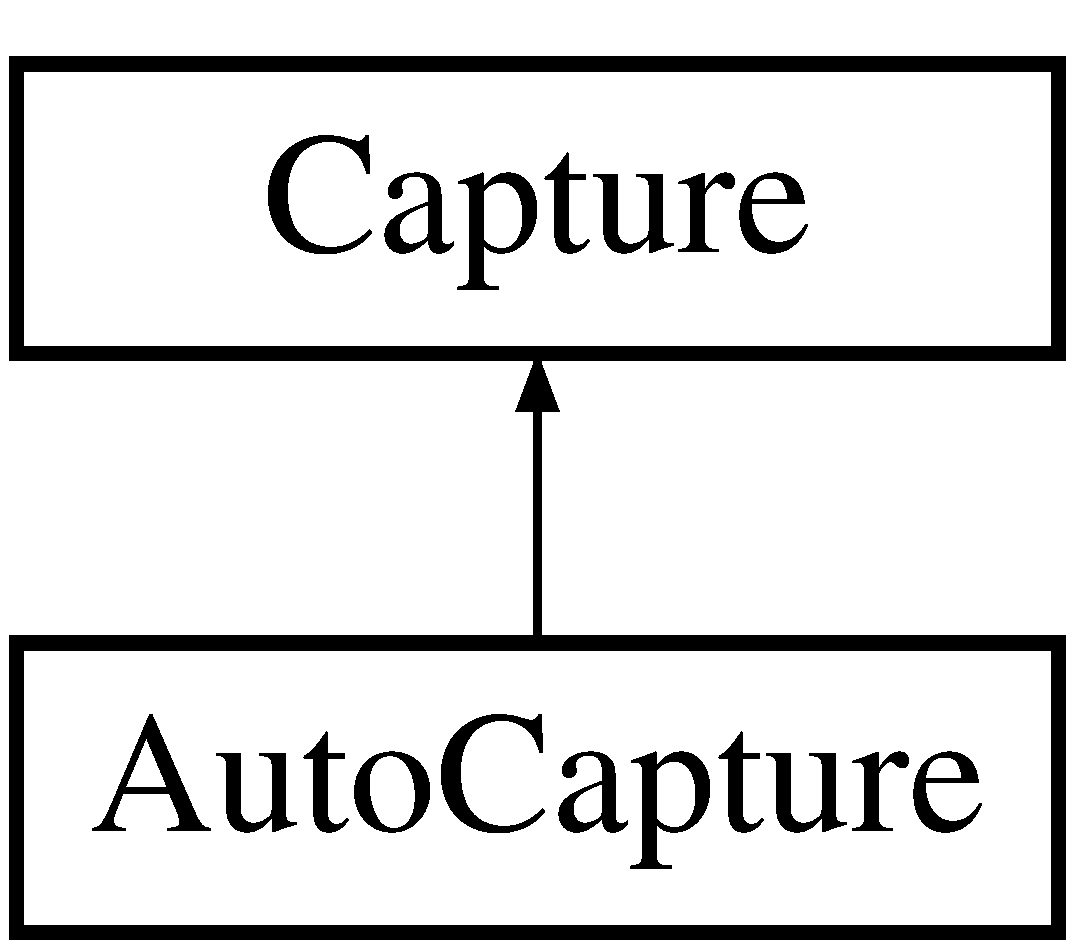
\includegraphics[height=2.000000cm]{class_auto_capture}
\end{center}
\end{figure}
\subsection*{Public Member Functions}
\begin{DoxyCompactItemize}
\item 
\hyperlink{class_auto_capture_acaabce59abc33a0b488fb84c196c1a9e}{Auto\+Capture} (\hyperlink{class_e_p_analysis}{E\+P\+Analysis} $\ast$\hyperlink{class_auto_capture_a7527bcbfe6636e4e34b3b0724d22ab5c}{ep})
\item 
\hyperlink{class_auto_capture_abe4754e9dd597d38f8d15fbdd8a39339}{$\sim$\+Auto\+Capture} ()
\item 
bool \hyperlink{class_auto_capture_ab5dc241ceb0226dcb2a17a3b56646210}{capture\+Action} (\hyperlink{class_raw_data}{Raw\+Data} $\ast$\hyperlink{readwave_8h_aa12fa7025612e5f4774f2412dd7f465b}{data})
\item 
bool \hyperlink{class_auto_capture_a39edd9a81495af7491701ef7b491a2bc}{init\+\_\+callback} (\hyperlink{class_raw_data}{Raw\+Data} $\ast$\hyperlink{readwave_8h_aa12fa7025612e5f4774f2412dd7f465b}{data}, bool input)
\end{DoxyCompactItemize}
\subsection*{Protected Attributes}
\begin{DoxyCompactItemize}
\item 
\hyperlink{class_e_p_analysis}{E\+P\+Analysis} $\ast$ \hyperlink{class_auto_capture_a7527bcbfe6636e4e34b3b0724d22ab5c}{ep}
\end{DoxyCompactItemize}
\subsection*{Additional Inherited Members}


\subsection{Constructor \& Destructor Documentation}
\hypertarget{class_auto_capture_acaabce59abc33a0b488fb84c196c1a9e}{\index{Auto\+Capture@{Auto\+Capture}!Auto\+Capture@{Auto\+Capture}}
\index{Auto\+Capture@{Auto\+Capture}!Auto\+Capture@{Auto\+Capture}}
\subsubsection[{Auto\+Capture}]{\setlength{\rightskip}{0pt plus 5cm}Auto\+Capture\+::\+Auto\+Capture (
\begin{DoxyParamCaption}
\item[{{\bf E\+P\+Analysis} $\ast$}]{ep}
\end{DoxyParamCaption}
)\hspace{0.3cm}{\ttfamily [inline]}}}\label{class_auto_capture_acaabce59abc33a0b488fb84c196c1a9e}
\hypertarget{class_auto_capture_abe4754e9dd597d38f8d15fbdd8a39339}{\index{Auto\+Capture@{Auto\+Capture}!````~Auto\+Capture@{$\sim$\+Auto\+Capture}}
\index{````~Auto\+Capture@{$\sim$\+Auto\+Capture}!Auto\+Capture@{Auto\+Capture}}
\subsubsection[{$\sim$\+Auto\+Capture}]{\setlength{\rightskip}{0pt plus 5cm}Auto\+Capture\+::$\sim$\+Auto\+Capture (
\begin{DoxyParamCaption}
{}
\end{DoxyParamCaption}
)\hspace{0.3cm}{\ttfamily [inline]}}}\label{class_auto_capture_abe4754e9dd597d38f8d15fbdd8a39339}


\subsection{Member Function Documentation}
\hypertarget{class_auto_capture_ab5dc241ceb0226dcb2a17a3b56646210}{\index{Auto\+Capture@{Auto\+Capture}!capture\+Action@{capture\+Action}}
\index{capture\+Action@{capture\+Action}!Auto\+Capture@{Auto\+Capture}}
\subsubsection[{capture\+Action}]{\setlength{\rightskip}{0pt plus 5cm}bool Auto\+Capture\+::capture\+Action (
\begin{DoxyParamCaption}
\item[{{\bf Raw\+Data} $\ast$}]{data}
\end{DoxyParamCaption}
)\hspace{0.3cm}{\ttfamily [virtual]}}}\label{class_auto_capture_ab5dc241ceb0226dcb2a17a3b56646210}


Reimplemented from \hyperlink{class_capture_afbd312bfcb81305f9bc542c56e83d64c}{Capture}.

\hypertarget{class_auto_capture_a39edd9a81495af7491701ef7b491a2bc}{\index{Auto\+Capture@{Auto\+Capture}!init\+\_\+callback@{init\+\_\+callback}}
\index{init\+\_\+callback@{init\+\_\+callback}!Auto\+Capture@{Auto\+Capture}}
\subsubsection[{init\+\_\+callback}]{\setlength{\rightskip}{0pt plus 5cm}bool Auto\+Capture\+::init\+\_\+callback (
\begin{DoxyParamCaption}
\item[{{\bf Raw\+Data} $\ast$}]{data, }
\item[{bool}]{input}
\end{DoxyParamCaption}
)\hspace{0.3cm}{\ttfamily [virtual]}}}\label{class_auto_capture_a39edd9a81495af7491701ef7b491a2bc}


Reimplemented from \hyperlink{class_capture_a646039c1a6c861683f547dd894ef4b27}{Capture}.



\subsection{Member Data Documentation}
\hypertarget{class_auto_capture_a7527bcbfe6636e4e34b3b0724d22ab5c}{\index{Auto\+Capture@{Auto\+Capture}!ep@{ep}}
\index{ep@{ep}!Auto\+Capture@{Auto\+Capture}}
\subsubsection[{ep}]{\setlength{\rightskip}{0pt plus 5cm}{\bf E\+P\+Analysis}$\ast$ Auto\+Capture\+::ep\hspace{0.3cm}{\ttfamily [protected]}}}\label{class_auto_capture_a7527bcbfe6636e4e34b3b0724d22ab5c}


The documentation for this class was generated from the following files\+:\begin{DoxyCompactItemize}
\item 
src/\+Capture/\hyperlink{_auto_capture_8h}{Auto\+Capture.\+h}\item 
src/\+Capture/\hyperlink{_auto_capture_8cpp}{Auto\+Capture.\+cpp}\end{DoxyCompactItemize}

\hypertarget{struct_back_ptr}{\section{Back\+Ptr Struct Reference}
\label{struct_back_ptr}\index{Back\+Ptr@{Back\+Ptr}}
}


{\ttfamily \#include $<$Seq\+Model.\+h$>$}

\subsection*{Public Attributes}
\begin{DoxyCompactItemize}
\item 
int \hyperlink{struct_back_ptr_a2adab93b217084150a956bf9c28e48a8}{state\+I\+D}
\item 
const char $\ast$ \hyperlink{struct_back_ptr_ab6ca867e253d7cfb09944b6e248af63a}{word}
\item 
int \hyperlink{struct_back_ptr_a6465b7c1e40c878c73dbba8fc7f5561f}{pre\+Ptr}
\end{DoxyCompactItemize}


\subsection{Member Data Documentation}
\hypertarget{struct_back_ptr_a6465b7c1e40c878c73dbba8fc7f5561f}{\index{Back\+Ptr@{Back\+Ptr}!pre\+Ptr@{pre\+Ptr}}
\index{pre\+Ptr@{pre\+Ptr}!Back\+Ptr@{Back\+Ptr}}
\subsubsection[{pre\+Ptr}]{\setlength{\rightskip}{0pt plus 5cm}int Back\+Ptr\+::pre\+Ptr}}\label{struct_back_ptr_a6465b7c1e40c878c73dbba8fc7f5561f}
\hypertarget{struct_back_ptr_a2adab93b217084150a956bf9c28e48a8}{\index{Back\+Ptr@{Back\+Ptr}!state\+I\+D@{state\+I\+D}}
\index{state\+I\+D@{state\+I\+D}!Back\+Ptr@{Back\+Ptr}}
\subsubsection[{state\+I\+D}]{\setlength{\rightskip}{0pt plus 5cm}int Back\+Ptr\+::state\+I\+D}}\label{struct_back_ptr_a2adab93b217084150a956bf9c28e48a8}
\hypertarget{struct_back_ptr_ab6ca867e253d7cfb09944b6e248af63a}{\index{Back\+Ptr@{Back\+Ptr}!word@{word}}
\index{word@{word}!Back\+Ptr@{Back\+Ptr}}
\subsubsection[{word}]{\setlength{\rightskip}{0pt plus 5cm}const char$\ast$ Back\+Ptr\+::word}}\label{struct_back_ptr_ab6ca867e253d7cfb09944b6e248af63a}


The documentation for this struct was generated from the following file\+:\begin{DoxyCompactItemize}
\item 
src/\+Feature/\hyperlink{_seq_model_8h}{Seq\+Model.\+h}\end{DoxyCompactItemize}

\hypertarget{class_b_e_p_analysis}{\section{B\+E\+P\+Analysis Class Reference}
\label{class_b_e_p_analysis}\index{B\+E\+P\+Analysis@{B\+E\+P\+Analysis}}
}


{\ttfamily \#include $<$B\+E\+P\+Analysis.\+h$>$}

Inheritance diagram for B\+E\+P\+Analysis\+:\begin{figure}[H]
\begin{center}
\leavevmode
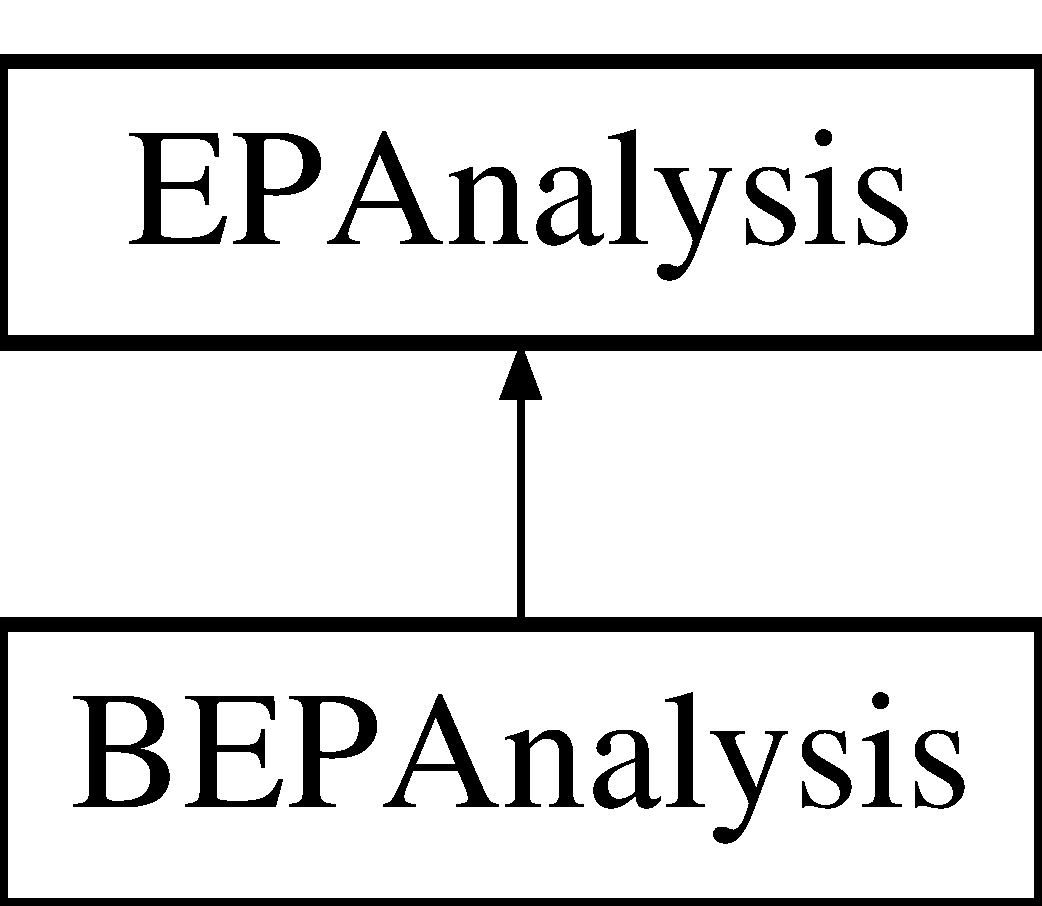
\includegraphics[height=2.000000cm]{class_b_e_p_analysis}
\end{center}
\end{figure}
\subsection*{Public Member Functions}
\begin{DoxyCompactItemize}
\item 
\hyperlink{class_b_e_p_analysis_ae1535efdce6c76552806f4877b344876}{B\+E\+P\+Analysis} ()
\item 
\hyperlink{class_b_e_p_analysis_acc98219f135576547fcd68e39e856e8a}{$\sim$\+B\+E\+P\+Analysis} ()
\end{DoxyCompactItemize}
\subsection*{Protected Member Functions}
\begin{DoxyCompactItemize}
\item 
virtual void \hyperlink{class_b_e_p_analysis_ace11d41c17bd9fbbbdddb85ccccb070e}{calc\+One\+Block\+Background} (int index)
\item 
virtual void \hyperlink{class_b_e_p_analysis_ab508a682d38fbc58319ea48bfaa54615}{calc\+One\+Block\+Speech} (int index)
\end{DoxyCompactItemize}
\subsection*{Additional Inherited Members}


\subsection{Constructor \& Destructor Documentation}
\hypertarget{class_b_e_p_analysis_ae1535efdce6c76552806f4877b344876}{\index{B\+E\+P\+Analysis@{B\+E\+P\+Analysis}!B\+E\+P\+Analysis@{B\+E\+P\+Analysis}}
\index{B\+E\+P\+Analysis@{B\+E\+P\+Analysis}!B\+E\+P\+Analysis@{B\+E\+P\+Analysis}}
\subsubsection[{B\+E\+P\+Analysis}]{\setlength{\rightskip}{0pt plus 5cm}B\+E\+P\+Analysis\+::\+B\+E\+P\+Analysis (
\begin{DoxyParamCaption}
{}
\end{DoxyParamCaption}
)\hspace{0.3cm}{\ttfamily [inline]}}}\label{class_b_e_p_analysis_ae1535efdce6c76552806f4877b344876}
\hypertarget{class_b_e_p_analysis_acc98219f135576547fcd68e39e856e8a}{\index{B\+E\+P\+Analysis@{B\+E\+P\+Analysis}!````~B\+E\+P\+Analysis@{$\sim$\+B\+E\+P\+Analysis}}
\index{````~B\+E\+P\+Analysis@{$\sim$\+B\+E\+P\+Analysis}!B\+E\+P\+Analysis@{B\+E\+P\+Analysis}}
\subsubsection[{$\sim$\+B\+E\+P\+Analysis}]{\setlength{\rightskip}{0pt plus 5cm}B\+E\+P\+Analysis\+::$\sim$\+B\+E\+P\+Analysis (
\begin{DoxyParamCaption}
{}
\end{DoxyParamCaption}
)\hspace{0.3cm}{\ttfamily [inline]}}}\label{class_b_e_p_analysis_acc98219f135576547fcd68e39e856e8a}


\subsection{Member Function Documentation}
\hypertarget{class_b_e_p_analysis_ace11d41c17bd9fbbbdddb85ccccb070e}{\index{B\+E\+P\+Analysis@{B\+E\+P\+Analysis}!calc\+One\+Block\+Background@{calc\+One\+Block\+Background}}
\index{calc\+One\+Block\+Background@{calc\+One\+Block\+Background}!B\+E\+P\+Analysis@{B\+E\+P\+Analysis}}
\subsubsection[{calc\+One\+Block\+Background}]{\setlength{\rightskip}{0pt plus 5cm}void B\+E\+P\+Analysis\+::calc\+One\+Block\+Background (
\begin{DoxyParamCaption}
\item[{int}]{index}
\end{DoxyParamCaption}
)\hspace{0.3cm}{\ttfamily [protected]}, {\ttfamily [virtual]}}}\label{class_b_e_p_analysis_ace11d41c17bd9fbbbdddb85ccccb070e}


Implements \hyperlink{class_e_p_analysis_ac0d297dde8d0e9663f2e2e3b5fa0bc39}{E\+P\+Analysis}.

\hypertarget{class_b_e_p_analysis_ab508a682d38fbc58319ea48bfaa54615}{\index{B\+E\+P\+Analysis@{B\+E\+P\+Analysis}!calc\+One\+Block\+Speech@{calc\+One\+Block\+Speech}}
\index{calc\+One\+Block\+Speech@{calc\+One\+Block\+Speech}!B\+E\+P\+Analysis@{B\+E\+P\+Analysis}}
\subsubsection[{calc\+One\+Block\+Speech}]{\setlength{\rightskip}{0pt plus 5cm}void B\+E\+P\+Analysis\+::calc\+One\+Block\+Speech (
\begin{DoxyParamCaption}
\item[{int}]{index}
\end{DoxyParamCaption}
)\hspace{0.3cm}{\ttfamily [protected]}, {\ttfamily [virtual]}}}\label{class_b_e_p_analysis_ab508a682d38fbc58319ea48bfaa54615}


Implements \hyperlink{class_e_p_analysis_a7767c0329b482231ec33faf935a620ce}{E\+P\+Analysis}.



The documentation for this class was generated from the following files\+:\begin{DoxyCompactItemize}
\item 
src/\+Analysis/\hyperlink{_b_e_p_analysis_8h}{B\+E\+P\+Analysis.\+h}\item 
src/\+Analysis/\hyperlink{_b_e_p_analysis_8cpp}{B\+E\+P\+Analysis.\+cpp}\end{DoxyCompactItemize}

\hypertarget{class_capture}{\section{Capture Class Reference}
\label{class_capture}\index{Capture@{Capture}}
}


{\ttfamily \#include $<$Capture.\+h$>$}

Inheritance diagram for Capture\+:\begin{figure}[H]
\begin{center}
\leavevmode
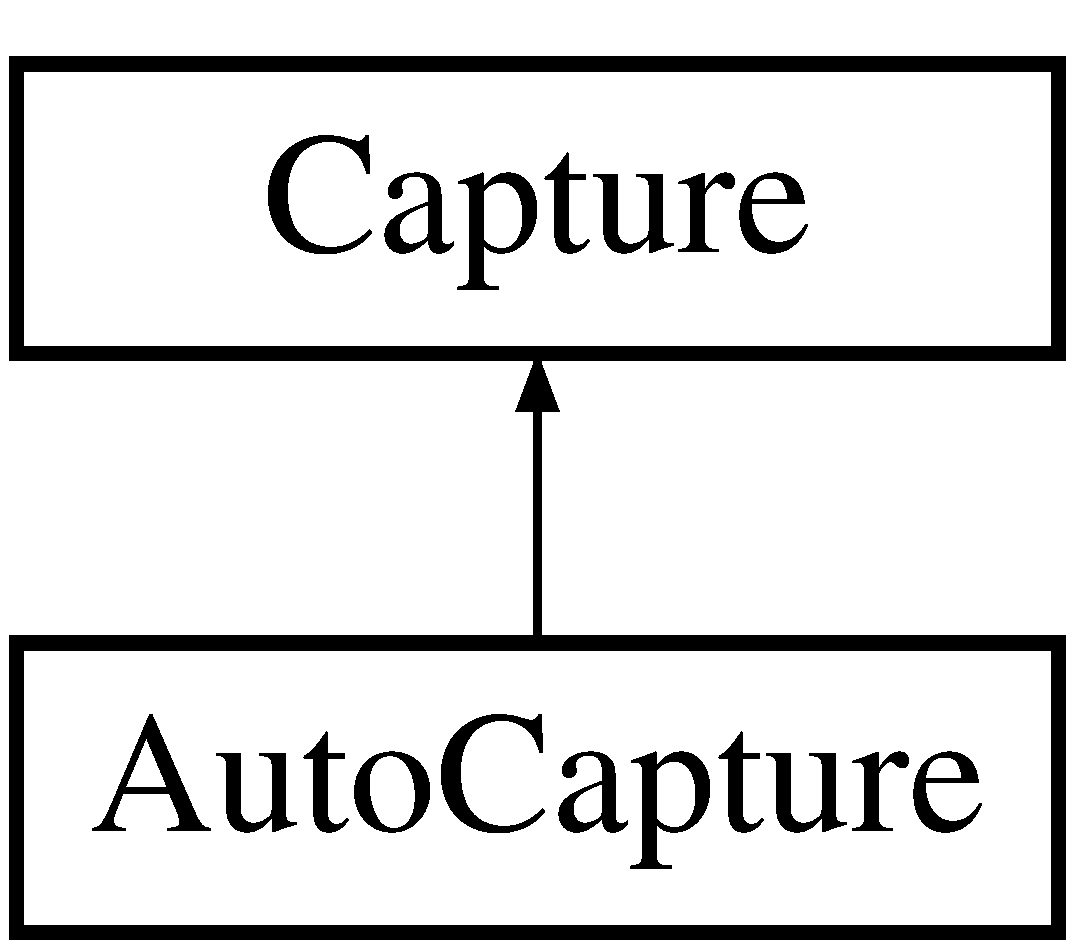
\includegraphics[height=2.000000cm]{class_capture}
\end{center}
\end{figure}
\subsection*{Public Member Functions}
\begin{DoxyCompactItemize}
\item 
\hyperlink{class_capture_a97036b5d271238bd4852da79a0091b57}{Capture} ()
\item 
\hyperlink{class_capture_ab5b3fac467fa47592126d782f9375250}{$\sim$\+Capture} ()
\item 
bool \hyperlink{class_capture_a3093205d35063cabcc642f2f1974298e}{capture} (\hyperlink{class_raw_data}{Raw\+Data} $\ast$)
\item 
bool \hyperlink{class_capture_a255daf1ddd78a6593b0e4850b39a9ec9}{play} (\hyperlink{class_raw_data}{Raw\+Data} $\ast$)
\end{DoxyCompactItemize}
\subsection*{Static Public Member Functions}
\begin{DoxyCompactItemize}
\item 
static \hyperlink{tool_8h_ab71a1f2fb85a32402ced5c483105b38e}{S\+P\+\_\+\+R\+E\+S\+U\+L\+T} \hyperlink{class_capture_a45364e6153b09910c64006b4dee2e3ba}{load\+\_\+wav\+\_\+file} (const char $\ast$const file\+\_\+name, \hyperlink{class_raw_data}{Raw\+Data} \&\hyperlink{readwave_8h_aa12fa7025612e5f4774f2412dd7f465b}{data}, bool \hyperlink{recorder_8cpp_afca07e4c3b4c5d94f98ac43562d19215}{playback}=false)
\end{DoxyCompactItemize}
\subsection*{Protected Member Functions}
\begin{DoxyCompactItemize}
\item 
bool \hyperlink{class_capture_ae88010511b90a237a8a17ad2a70e5432}{init\+\_\+stream} (bool input)
\item 
bool \hyperlink{class_capture_ae3ad177c3bd753d8ec633ac545f9b929}{init\+\_\+\+P\+A} ()
\item 
bool \hyperlink{class_capture_a30365cdef1c06d2e1f8cf7abba00b21f}{init} (\hyperlink{class_raw_data}{Raw\+Data} $\ast$\hyperlink{readwave_8h_aa12fa7025612e5f4774f2412dd7f465b}{data}, bool input)
\item 
bool \hyperlink{class_capture_a3ed2fabc0ab88e8b0dd9dc8b108cf0fb}{end} ()
\item 
virtual bool \hyperlink{class_capture_afbd312bfcb81305f9bc542c56e83d64c}{capture\+Action} (\hyperlink{class_raw_data}{Raw\+Data} $\ast$\hyperlink{readwave_8h_aa12fa7025612e5f4774f2412dd7f465b}{data})
\item 
virtual bool \hyperlink{class_capture_a4dea1091e735509dd97e0b14e054f77f}{play\+Action} (\hyperlink{class_raw_data}{Raw\+Data} $\ast$\hyperlink{readwave_8h_aa12fa7025612e5f4774f2412dd7f465b}{data})
\item 
virtual bool \hyperlink{class_capture_a646039c1a6c861683f547dd894ef4b27}{init\+\_\+callback} (\hyperlink{class_raw_data}{Raw\+Data} $\ast$\hyperlink{readwave_8h_aa12fa7025612e5f4774f2412dd7f465b}{data}, bool input)
\end{DoxyCompactItemize}
\subsection*{Protected Attributes}
\begin{DoxyCompactItemize}
\item 
Pa\+Stream\+Parameters \hyperlink{class_capture_a84320acc014a2d81574a876e6d693108}{in}
\item 
Pa\+Stream\+Parameters \hyperlink{class_capture_ad9e4da58dead277ef3b387fd4080d12b}{out}
\item 
Pa\+Stream $\ast$ \hyperlink{class_capture_abc592c61bc547b65c395b8a43c5cf1ad}{stream}
\item 
Pa\+Stream\+Callback $\ast$ \hyperlink{class_capture_a8011f682b8e253387a717134b454c2d4}{callback}
\item 
void $\ast$ \hyperlink{class_capture_a0253ca7959f1e3a550502c33612e3c2e}{user\+Data}
\end{DoxyCompactItemize}


\subsection{Constructor \& Destructor Documentation}
\hypertarget{class_capture_a97036b5d271238bd4852da79a0091b57}{\index{Capture@{Capture}!Capture@{Capture}}
\index{Capture@{Capture}!Capture@{Capture}}
\subsubsection[{Capture}]{\setlength{\rightskip}{0pt plus 5cm}Capture\+::\+Capture (
\begin{DoxyParamCaption}
{}
\end{DoxyParamCaption}
)}}\label{class_capture_a97036b5d271238bd4852da79a0091b57}
\hypertarget{class_capture_ab5b3fac467fa47592126d782f9375250}{\index{Capture@{Capture}!````~Capture@{$\sim$\+Capture}}
\index{````~Capture@{$\sim$\+Capture}!Capture@{Capture}}
\subsubsection[{$\sim$\+Capture}]{\setlength{\rightskip}{0pt plus 5cm}Capture\+::$\sim$\+Capture (
\begin{DoxyParamCaption}
{}
\end{DoxyParamCaption}
)}}\label{class_capture_ab5b3fac467fa47592126d782f9375250}


\subsection{Member Function Documentation}
\hypertarget{class_capture_a3093205d35063cabcc642f2f1974298e}{\index{Capture@{Capture}!capture@{capture}}
\index{capture@{capture}!Capture@{Capture}}
\subsubsection[{capture}]{\setlength{\rightskip}{0pt plus 5cm}bool Capture\+::capture (
\begin{DoxyParamCaption}
\item[{{\bf Raw\+Data} $\ast$}]{data}
\end{DoxyParamCaption}
)}}\label{class_capture_a3093205d35063cabcc642f2f1974298e}
\hypertarget{class_capture_afbd312bfcb81305f9bc542c56e83d64c}{\index{Capture@{Capture}!capture\+Action@{capture\+Action}}
\index{capture\+Action@{capture\+Action}!Capture@{Capture}}
\subsubsection[{capture\+Action}]{\setlength{\rightskip}{0pt plus 5cm}bool Capture\+::capture\+Action (
\begin{DoxyParamCaption}
\item[{{\bf Raw\+Data} $\ast$}]{data}
\end{DoxyParamCaption}
)\hspace{0.3cm}{\ttfamily [protected]}, {\ttfamily [virtual]}}}\label{class_capture_afbd312bfcb81305f9bc542c56e83d64c}


Reimplemented in \hyperlink{class_auto_capture_ab5dc241ceb0226dcb2a17a3b56646210}{Auto\+Capture}.

\hypertarget{class_capture_a3ed2fabc0ab88e8b0dd9dc8b108cf0fb}{\index{Capture@{Capture}!end@{end}}
\index{end@{end}!Capture@{Capture}}
\subsubsection[{end}]{\setlength{\rightskip}{0pt plus 5cm}bool Capture\+::end (
\begin{DoxyParamCaption}
{}
\end{DoxyParamCaption}
)\hspace{0.3cm}{\ttfamily [protected]}}}\label{class_capture_a3ed2fabc0ab88e8b0dd9dc8b108cf0fb}
\hypertarget{class_capture_a30365cdef1c06d2e1f8cf7abba00b21f}{\index{Capture@{Capture}!init@{init}}
\index{init@{init}!Capture@{Capture}}
\subsubsection[{init}]{\setlength{\rightskip}{0pt plus 5cm}bool Capture\+::init (
\begin{DoxyParamCaption}
\item[{{\bf Raw\+Data} $\ast$}]{data, }
\item[{bool}]{input}
\end{DoxyParamCaption}
)\hspace{0.3cm}{\ttfamily [protected]}}}\label{class_capture_a30365cdef1c06d2e1f8cf7abba00b21f}
\hypertarget{class_capture_a646039c1a6c861683f547dd894ef4b27}{\index{Capture@{Capture}!init\+\_\+callback@{init\+\_\+callback}}
\index{init\+\_\+callback@{init\+\_\+callback}!Capture@{Capture}}
\subsubsection[{init\+\_\+callback}]{\setlength{\rightskip}{0pt plus 5cm}bool Capture\+::init\+\_\+callback (
\begin{DoxyParamCaption}
\item[{{\bf Raw\+Data} $\ast$}]{data, }
\item[{bool}]{input}
\end{DoxyParamCaption}
)\hspace{0.3cm}{\ttfamily [protected]}, {\ttfamily [virtual]}}}\label{class_capture_a646039c1a6c861683f547dd894ef4b27}


Reimplemented in \hyperlink{class_auto_capture_a39edd9a81495af7491701ef7b491a2bc}{Auto\+Capture}.

\hypertarget{class_capture_ae3ad177c3bd753d8ec633ac545f9b929}{\index{Capture@{Capture}!init\+\_\+\+P\+A@{init\+\_\+\+P\+A}}
\index{init\+\_\+\+P\+A@{init\+\_\+\+P\+A}!Capture@{Capture}}
\subsubsection[{init\+\_\+\+P\+A}]{\setlength{\rightskip}{0pt plus 5cm}bool Capture\+::init\+\_\+\+P\+A (
\begin{DoxyParamCaption}
{}
\end{DoxyParamCaption}
)\hspace{0.3cm}{\ttfamily [protected]}}}\label{class_capture_ae3ad177c3bd753d8ec633ac545f9b929}
\hypertarget{class_capture_ae88010511b90a237a8a17ad2a70e5432}{\index{Capture@{Capture}!init\+\_\+stream@{init\+\_\+stream}}
\index{init\+\_\+stream@{init\+\_\+stream}!Capture@{Capture}}
\subsubsection[{init\+\_\+stream}]{\setlength{\rightskip}{0pt plus 5cm}bool Capture\+::init\+\_\+stream (
\begin{DoxyParamCaption}
\item[{bool}]{input}
\end{DoxyParamCaption}
)\hspace{0.3cm}{\ttfamily [protected]}}}\label{class_capture_ae88010511b90a237a8a17ad2a70e5432}
\hypertarget{class_capture_a45364e6153b09910c64006b4dee2e3ba}{\index{Capture@{Capture}!load\+\_\+wav\+\_\+file@{load\+\_\+wav\+\_\+file}}
\index{load\+\_\+wav\+\_\+file@{load\+\_\+wav\+\_\+file}!Capture@{Capture}}
\subsubsection[{load\+\_\+wav\+\_\+file}]{\setlength{\rightskip}{0pt plus 5cm}static {\bf S\+P\+\_\+\+R\+E\+S\+U\+L\+T} Capture\+::load\+\_\+wav\+\_\+file (
\begin{DoxyParamCaption}
\item[{const char $\ast$const}]{file\+\_\+name, }
\item[{{\bf Raw\+Data} \&}]{data, }
\item[{bool}]{playback = {\ttfamily false}}
\end{DoxyParamCaption}
)\hspace{0.3cm}{\ttfamily [inline]}, {\ttfamily [static]}}}\label{class_capture_a45364e6153b09910c64006b4dee2e3ba}
\hypertarget{class_capture_a255daf1ddd78a6593b0e4850b39a9ec9}{\index{Capture@{Capture}!play@{play}}
\index{play@{play}!Capture@{Capture}}
\subsubsection[{play}]{\setlength{\rightskip}{0pt plus 5cm}bool Capture\+::play (
\begin{DoxyParamCaption}
\item[{{\bf Raw\+Data} $\ast$}]{data}
\end{DoxyParamCaption}
)}}\label{class_capture_a255daf1ddd78a6593b0e4850b39a9ec9}
\hypertarget{class_capture_a4dea1091e735509dd97e0b14e054f77f}{\index{Capture@{Capture}!play\+Action@{play\+Action}}
\index{play\+Action@{play\+Action}!Capture@{Capture}}
\subsubsection[{play\+Action}]{\setlength{\rightskip}{0pt plus 5cm}bool Capture\+::play\+Action (
\begin{DoxyParamCaption}
\item[{{\bf Raw\+Data} $\ast$}]{data}
\end{DoxyParamCaption}
)\hspace{0.3cm}{\ttfamily [protected]}, {\ttfamily [virtual]}}}\label{class_capture_a4dea1091e735509dd97e0b14e054f77f}


\subsection{Member Data Documentation}
\hypertarget{class_capture_a8011f682b8e253387a717134b454c2d4}{\index{Capture@{Capture}!callback@{callback}}
\index{callback@{callback}!Capture@{Capture}}
\subsubsection[{callback}]{\setlength{\rightskip}{0pt plus 5cm}Pa\+Stream\+Callback$\ast$ Capture\+::callback\hspace{0.3cm}{\ttfamily [protected]}}}\label{class_capture_a8011f682b8e253387a717134b454c2d4}
\hypertarget{class_capture_a84320acc014a2d81574a876e6d693108}{\index{Capture@{Capture}!in@{in}}
\index{in@{in}!Capture@{Capture}}
\subsubsection[{in}]{\setlength{\rightskip}{0pt plus 5cm}Pa\+Stream\+Parameters Capture\+::in\hspace{0.3cm}{\ttfamily [protected]}}}\label{class_capture_a84320acc014a2d81574a876e6d693108}
\hypertarget{class_capture_ad9e4da58dead277ef3b387fd4080d12b}{\index{Capture@{Capture}!out@{out}}
\index{out@{out}!Capture@{Capture}}
\subsubsection[{out}]{\setlength{\rightskip}{0pt plus 5cm}Pa\+Stream\+Parameters Capture\+::out\hspace{0.3cm}{\ttfamily [protected]}}}\label{class_capture_ad9e4da58dead277ef3b387fd4080d12b}
\hypertarget{class_capture_abc592c61bc547b65c395b8a43c5cf1ad}{\index{Capture@{Capture}!stream@{stream}}
\index{stream@{stream}!Capture@{Capture}}
\subsubsection[{stream}]{\setlength{\rightskip}{0pt plus 5cm}Pa\+Stream$\ast$ Capture\+::stream\hspace{0.3cm}{\ttfamily [protected]}}}\label{class_capture_abc592c61bc547b65c395b8a43c5cf1ad}
\hypertarget{class_capture_a0253ca7959f1e3a550502c33612e3c2e}{\index{Capture@{Capture}!user\+Data@{user\+Data}}
\index{user\+Data@{user\+Data}!Capture@{Capture}}
\subsubsection[{user\+Data}]{\setlength{\rightskip}{0pt plus 5cm}void$\ast$ Capture\+::user\+Data\hspace{0.3cm}{\ttfamily [protected]}}}\label{class_capture_a0253ca7959f1e3a550502c33612e3c2e}


The documentation for this class was generated from the following files\+:\begin{DoxyCompactItemize}
\item 
src/\+Capture/\hyperlink{_capture_8h}{Capture.\+h}\item 
src/\+Capture/\hyperlink{_capture_8cpp}{Capture.\+cpp}\end{DoxyCompactItemize}

\hypertarget{struct_cluster}{\section{Cluster Struct Reference}
\label{struct_cluster}\index{Cluster@{Cluster}}
}


{\ttfamily \#include $<$K\+Mean\+State.\+h$>$}

\subsection*{Public Attributes}
\begin{DoxyCompactItemize}
\item 
\hyperlink{class_gaussian}{Gaussian} $\ast$ \hyperlink{struct_cluster_affaced9bc07c578318f59592d18c68b8}{g}
\item 
std\+::vector$<$ \hyperlink{class_feature}{Feature} $\ast$ $>$ \hyperlink{struct_cluster_aeffb52e9b39090a30dd621965ec577ae}{points}
\item 
double \hyperlink{struct_cluster_ab79e9b6fda34ac8768122889048304ba}{w}
\end{DoxyCompactItemize}


\subsection{Member Data Documentation}
\hypertarget{struct_cluster_affaced9bc07c578318f59592d18c68b8}{\index{Cluster@{Cluster}!g@{g}}
\index{g@{g}!Cluster@{Cluster}}
\subsubsection[{g}]{\setlength{\rightskip}{0pt plus 5cm}{\bf Gaussian}$\ast$ Cluster\+::g}}\label{struct_cluster_affaced9bc07c578318f59592d18c68b8}
\hypertarget{struct_cluster_aeffb52e9b39090a30dd621965ec577ae}{\index{Cluster@{Cluster}!points@{points}}
\index{points@{points}!Cluster@{Cluster}}
\subsubsection[{points}]{\setlength{\rightskip}{0pt plus 5cm}std\+::vector$<${\bf Feature}$\ast$$>$ Cluster\+::points}}\label{struct_cluster_aeffb52e9b39090a30dd621965ec577ae}
\hypertarget{struct_cluster_ab79e9b6fda34ac8768122889048304ba}{\index{Cluster@{Cluster}!w@{w}}
\index{w@{w}!Cluster@{Cluster}}
\subsubsection[{w}]{\setlength{\rightskip}{0pt plus 5cm}double Cluster\+::w}}\label{struct_cluster_ab79e9b6fda34ac8768122889048304ba}


The documentation for this struct was generated from the following file\+:\begin{DoxyCompactItemize}
\item 
src/\+Feature/\hyperlink{_k_mean_state_8h}{K\+Mean\+State.\+h}\end{DoxyCompactItemize}

\hypertarget{structcmp__task__info}{\section{cmp\+\_\+task\+\_\+info Struct Reference}
\label{structcmp__task__info}\index{cmp\+\_\+task\+\_\+info@{cmp\+\_\+task\+\_\+info}}
}


{\ttfamily \#include $<$app.\+h$>$}

\subsection*{Public Attributes}
\begin{DoxyCompactItemize}
\item 
int \hyperlink{structcmp__task__info_a3633d922d3eef29d9ebb03ca51010b8f}{index}
\item 
const char $\ast$ \hyperlink{structcmp__task__info_a4539e63c72404966130c3129cd71aa8d}{w}
\item 
vector$<$ string $>$ $\ast$ \hyperlink{structcmp__task__info_ae886fd2b9fa914fd8937ff6aea779234}{dict}
\item 
vector$<$ int $>$ $\ast$ \hyperlink{structcmp__task__info_acf3590e23bc8a1c548ffa74a7c5d794c}{result}
\item 
int \hyperlink{structcmp__task__info_a96314bf00c0c73e503a81ecdcd6502be}{type}
\item 
\hyperlink{struct_path}{Path} $\ast$ \hyperlink{structcmp__task__info_ad0c6b8c7f0797b2043dba88d679d8f2f}{p}
\end{DoxyCompactItemize}


\subsection{Member Data Documentation}
\hypertarget{structcmp__task__info_ae886fd2b9fa914fd8937ff6aea779234}{\index{cmp\+\_\+task\+\_\+info@{cmp\+\_\+task\+\_\+info}!dict@{dict}}
\index{dict@{dict}!cmp\+\_\+task\+\_\+info@{cmp\+\_\+task\+\_\+info}}
\subsubsection[{dict}]{\setlength{\rightskip}{0pt plus 5cm}vector$<$ string $>$ $\ast$ cmp\+\_\+task\+\_\+info\+::dict}}\label{structcmp__task__info_ae886fd2b9fa914fd8937ff6aea779234}
\hypertarget{structcmp__task__info_a3633d922d3eef29d9ebb03ca51010b8f}{\index{cmp\+\_\+task\+\_\+info@{cmp\+\_\+task\+\_\+info}!index@{index}}
\index{index@{index}!cmp\+\_\+task\+\_\+info@{cmp\+\_\+task\+\_\+info}}
\subsubsection[{index}]{\setlength{\rightskip}{0pt plus 5cm}int cmp\+\_\+task\+\_\+info\+::index}}\label{structcmp__task__info_a3633d922d3eef29d9ebb03ca51010b8f}
\hypertarget{structcmp__task__info_ad0c6b8c7f0797b2043dba88d679d8f2f}{\index{cmp\+\_\+task\+\_\+info@{cmp\+\_\+task\+\_\+info}!p@{p}}
\index{p@{p}!cmp\+\_\+task\+\_\+info@{cmp\+\_\+task\+\_\+info}}
\subsubsection[{p}]{\setlength{\rightskip}{0pt plus 5cm}{\bf Path} $\ast$ cmp\+\_\+task\+\_\+info\+::p}}\label{structcmp__task__info_ad0c6b8c7f0797b2043dba88d679d8f2f}
\hypertarget{structcmp__task__info_acf3590e23bc8a1c548ffa74a7c5d794c}{\index{cmp\+\_\+task\+\_\+info@{cmp\+\_\+task\+\_\+info}!result@{result}}
\index{result@{result}!cmp\+\_\+task\+\_\+info@{cmp\+\_\+task\+\_\+info}}
\subsubsection[{result}]{\setlength{\rightskip}{0pt plus 5cm}vector$<$ int $>$ $\ast$ cmp\+\_\+task\+\_\+info\+::result}}\label{structcmp__task__info_acf3590e23bc8a1c548ffa74a7c5d794c}
\hypertarget{structcmp__task__info_a96314bf00c0c73e503a81ecdcd6502be}{\index{cmp\+\_\+task\+\_\+info@{cmp\+\_\+task\+\_\+info}!type@{type}}
\index{type@{type}!cmp\+\_\+task\+\_\+info@{cmp\+\_\+task\+\_\+info}}
\subsubsection[{type}]{\setlength{\rightskip}{0pt plus 5cm}int cmp\+\_\+task\+\_\+info\+::type}}\label{structcmp__task__info_a96314bf00c0c73e503a81ecdcd6502be}
\hypertarget{structcmp__task__info_a4539e63c72404966130c3129cd71aa8d}{\index{cmp\+\_\+task\+\_\+info@{cmp\+\_\+task\+\_\+info}!w@{w}}
\index{w@{w}!cmp\+\_\+task\+\_\+info@{cmp\+\_\+task\+\_\+info}}
\subsubsection[{w}]{\setlength{\rightskip}{0pt plus 5cm}const char $\ast$ cmp\+\_\+task\+\_\+info\+::w}}\label{structcmp__task__info_a4539e63c72404966130c3129cd71aa8d}


The documentation for this struct was generated from the following file\+:\begin{DoxyCompactItemize}
\item 
src/\+Edit\+Distance/\hyperlink{_edit_distance_2app_8h}{app.\+h}\end{DoxyCompactItemize}

\hypertarget{class_conf}{\section{Conf Class Reference}
\label{class_conf}\index{Conf@{Conf}}
}


{\ttfamily \#include $<$conf.\+h$>$}

\subsection*{Static Public Attributes}
\begin{DoxyCompactItemize}
\item 
static int \hyperlink{class_conf_a711f62286eebacda65e1ae8da7eaebd2}{threshold} = 3
\item 
static int \hyperlink{class_conf_a4c3c0b9e5ea26314911bf1e645779377}{beam} = 3
\item 
static int \hyperlink{class_conf_adba927d772295408e9c93e9b7bf30eb8}{info} = 0
\item 
static int \hyperlink{class_conf_a142f3e8a32431f0c5d2d1ed25a547979}{debug} = 0
\end{DoxyCompactItemize}


\subsection{Member Data Documentation}
\hypertarget{class_conf_a4c3c0b9e5ea26314911bf1e645779377}{\index{Conf@{Conf}!beam@{beam}}
\index{beam@{beam}!Conf@{Conf}}
\subsubsection[{beam}]{\setlength{\rightskip}{0pt plus 5cm}int Conf\+::beam = 3\hspace{0.3cm}{\ttfamily [static]}}}\label{class_conf_a4c3c0b9e5ea26314911bf1e645779377}
\hypertarget{class_conf_a142f3e8a32431f0c5d2d1ed25a547979}{\index{Conf@{Conf}!debug@{debug}}
\index{debug@{debug}!Conf@{Conf}}
\subsubsection[{debug}]{\setlength{\rightskip}{0pt plus 5cm}int Conf\+::debug = 0\hspace{0.3cm}{\ttfamily [static]}}}\label{class_conf_a142f3e8a32431f0c5d2d1ed25a547979}
\hypertarget{class_conf_adba927d772295408e9c93e9b7bf30eb8}{\index{Conf@{Conf}!info@{info}}
\index{info@{info}!Conf@{Conf}}
\subsubsection[{info}]{\setlength{\rightskip}{0pt plus 5cm}int Conf\+::info = 0\hspace{0.3cm}{\ttfamily [static]}}}\label{class_conf_adba927d772295408e9c93e9b7bf30eb8}
\hypertarget{class_conf_a711f62286eebacda65e1ae8da7eaebd2}{\index{Conf@{Conf}!threshold@{threshold}}
\index{threshold@{threshold}!Conf@{Conf}}
\subsubsection[{threshold}]{\setlength{\rightskip}{0pt plus 5cm}int Conf\+::threshold = 3\hspace{0.3cm}{\ttfamily [static]}}}\label{class_conf_a711f62286eebacda65e1ae8da7eaebd2}


The documentation for this class was generated from the following files\+:\begin{DoxyCompactItemize}
\item 
src/\+Edit\+Distance/\hyperlink{conf_8h}{conf.\+h}\item 
src/\hyperlink{pro3__demo_8cpp}{pro3\+\_\+demo.\+cpp}\end{DoxyCompactItemize}

\hypertarget{class_container}{\section{Container$<$ T $>$ Class Template Reference}
\label{class_container}\index{Container$<$ T $>$@{Container$<$ T $>$}}
}


{\ttfamily \#include $<$container.\+h$>$}

\subsection*{Public Member Functions}
\begin{DoxyCompactItemize}
\item 
\hyperlink{class_container_ab17ce1f67243b28abcd4c8113a72524c}{Container} ()
\item 
\hyperlink{class_container_a3588c5096f50a0a6020403bc5a5ca68b}{Container} (T $\ast$\hyperlink{class_container_adf060dcd6dfb12774aced955881149d8}{items}, int \hyperlink{class_container_a28ddede70f4d2c63b8571291b714d6ff}{len})
\item 
\hyperlink{class_container_a5b3440c3177017d2d6a190724e7078ec}{$\sim$\+Container} ()
\item 
bool \hyperlink{class_container_a2e97d3b9786e4b6ae9404a9f18ffe2fb}{check} (int \hyperlink{process__options_8m_a6f6ccfcf58b31cb6412107d9d5281426}{i}, const T \&a) const 
\item 
int \hyperlink{class_container_a28ddede70f4d2c63b8571291b714d6ff}{len} () const 
\item 
void \hyperlink{class_container_afb84989fc3eaa501fab06c148facd5e3}{add} (const T \&\hyperlink{readhtk_8m_aaccc9105df5383111407fd5b41255e23}{t})
\item 
const T \& \hyperlink{class_container_acbf6c7d4dbebe662467b35c7b0f48487}{operator\mbox{[}$\,$\mbox{]}} (int \hyperlink{readhtk_8m_aaccc9105df5383111407fd5b41255e23}{t}) const 
\end{DoxyCompactItemize}
\subsection*{Protected Attributes}
\begin{DoxyCompactItemize}
\item 
vector$<$ T $>$ \hyperlink{class_container_adf060dcd6dfb12774aced955881149d8}{items}
\end{DoxyCompactItemize}
\subsection*{Friends}
\begin{DoxyCompactItemize}
\item 
bool \hyperlink{class_container_a5f79f5574a200f0de7733d28852ddb99}{operator$<$} (const \hyperlink{class_container}{Container}$<$ T $>$ \&a, const \hyperlink{class_container}{Container}$<$ T $>$ \&b)
\item 
bool \hyperlink{class_container_a21fc06e1d8b2414882e2c0e65464c42b}{operator==} (const \hyperlink{class_container}{Container}$<$ T $>$ \&a, const \hyperlink{class_container}{Container}$<$ T $>$ \&b)
\end{DoxyCompactItemize}


\subsection{Constructor \& Destructor Documentation}
\hypertarget{class_container_ab17ce1f67243b28abcd4c8113a72524c}{\index{Container@{Container}!Container@{Container}}
\index{Container@{Container}!Container@{Container}}
\subsubsection[{Container}]{\setlength{\rightskip}{0pt plus 5cm}template$<$typename T$>$ {\bf Container}$<$ T $>$\+::{\bf Container} (
\begin{DoxyParamCaption}
{}
\end{DoxyParamCaption}
)\hspace{0.3cm}{\ttfamily [inline]}}}\label{class_container_ab17ce1f67243b28abcd4c8113a72524c}
\hypertarget{class_container_a3588c5096f50a0a6020403bc5a5ca68b}{\index{Container@{Container}!Container@{Container}}
\index{Container@{Container}!Container@{Container}}
\subsubsection[{Container}]{\setlength{\rightskip}{0pt plus 5cm}template$<$typename T$>$ {\bf Container}$<$ T $>$\+::{\bf Container} (
\begin{DoxyParamCaption}
\item[{T $\ast$}]{items, }
\item[{int}]{len}
\end{DoxyParamCaption}
)\hspace{0.3cm}{\ttfamily [inline]}}}\label{class_container_a3588c5096f50a0a6020403bc5a5ca68b}
\hypertarget{class_container_a5b3440c3177017d2d6a190724e7078ec}{\index{Container@{Container}!````~Container@{$\sim$\+Container}}
\index{````~Container@{$\sim$\+Container}!Container@{Container}}
\subsubsection[{$\sim$\+Container}]{\setlength{\rightskip}{0pt plus 5cm}template$<$typename T$>$ {\bf Container}$<$ T $>$\+::$\sim${\bf Container} (
\begin{DoxyParamCaption}
{}
\end{DoxyParamCaption}
)\hspace{0.3cm}{\ttfamily [inline]}}}\label{class_container_a5b3440c3177017d2d6a190724e7078ec}


\subsection{Member Function Documentation}
\hypertarget{class_container_afb84989fc3eaa501fab06c148facd5e3}{\index{Container@{Container}!add@{add}}
\index{add@{add}!Container@{Container}}
\subsubsection[{add}]{\setlength{\rightskip}{0pt plus 5cm}template$<$typename T$>$ void {\bf Container}$<$ T $>$\+::add (
\begin{DoxyParamCaption}
\item[{const T \&}]{t}
\end{DoxyParamCaption}
)\hspace{0.3cm}{\ttfamily [inline]}}}\label{class_container_afb84989fc3eaa501fab06c148facd5e3}
\hypertarget{class_container_a2e97d3b9786e4b6ae9404a9f18ffe2fb}{\index{Container@{Container}!check@{check}}
\index{check@{check}!Container@{Container}}
\subsubsection[{check}]{\setlength{\rightskip}{0pt plus 5cm}template$<$typename T$>$ bool {\bf Container}$<$ T $>$\+::check (
\begin{DoxyParamCaption}
\item[{int}]{i, }
\item[{const T \&}]{a}
\end{DoxyParamCaption}
) const\hspace{0.3cm}{\ttfamily [inline]}}}\label{class_container_a2e97d3b9786e4b6ae9404a9f18ffe2fb}
\hypertarget{class_container_a28ddede70f4d2c63b8571291b714d6ff}{\index{Container@{Container}!len@{len}}
\index{len@{len}!Container@{Container}}
\subsubsection[{len}]{\setlength{\rightskip}{0pt plus 5cm}template$<$typename T$>$ int {\bf Container}$<$ T $>$\+::len (
\begin{DoxyParamCaption}
{}
\end{DoxyParamCaption}
) const\hspace{0.3cm}{\ttfamily [inline]}}}\label{class_container_a28ddede70f4d2c63b8571291b714d6ff}
\hypertarget{class_container_acbf6c7d4dbebe662467b35c7b0f48487}{\index{Container@{Container}!operator\mbox{[}$\,$\mbox{]}@{operator[]}}
\index{operator\mbox{[}$\,$\mbox{]}@{operator[]}!Container@{Container}}
\subsubsection[{operator[]}]{\setlength{\rightskip}{0pt plus 5cm}template$<$typename T$>$ const T\& {\bf Container}$<$ T $>$\+::operator\mbox{[}$\,$\mbox{]} (
\begin{DoxyParamCaption}
\item[{int}]{t}
\end{DoxyParamCaption}
) const\hspace{0.3cm}{\ttfamily [inline]}}}\label{class_container_acbf6c7d4dbebe662467b35c7b0f48487}


\subsection{Friends And Related Function Documentation}
\hypertarget{class_container_a5f79f5574a200f0de7733d28852ddb99}{\index{Container@{Container}!operator$<$@{operator$<$}}
\index{operator$<$@{operator$<$}!Container@{Container}}
\subsubsection[{operator$<$}]{\setlength{\rightskip}{0pt plus 5cm}template$<$typename T$>$ bool operator$<$ (
\begin{DoxyParamCaption}
\item[{const {\bf Container}$<$ T $>$ \&}]{a, }
\item[{const {\bf Container}$<$ T $>$ \&}]{b}
\end{DoxyParamCaption}
)\hspace{0.3cm}{\ttfamily [friend]}}}\label{class_container_a5f79f5574a200f0de7733d28852ddb99}
\hypertarget{class_container_a21fc06e1d8b2414882e2c0e65464c42b}{\index{Container@{Container}!operator==@{operator==}}
\index{operator==@{operator==}!Container@{Container}}
\subsubsection[{operator==}]{\setlength{\rightskip}{0pt plus 5cm}template$<$typename T$>$ bool operator== (
\begin{DoxyParamCaption}
\item[{const {\bf Container}$<$ T $>$ \&}]{a, }
\item[{const {\bf Container}$<$ T $>$ \&}]{b}
\end{DoxyParamCaption}
)\hspace{0.3cm}{\ttfamily [friend]}}}\label{class_container_a21fc06e1d8b2414882e2c0e65464c42b}


\subsection{Member Data Documentation}
\hypertarget{class_container_adf060dcd6dfb12774aced955881149d8}{\index{Container@{Container}!items@{items}}
\index{items@{items}!Container@{Container}}
\subsubsection[{items}]{\setlength{\rightskip}{0pt plus 5cm}template$<$typename T$>$ vector$<$T$>$ {\bf Container}$<$ T $>$\+::items\hspace{0.3cm}{\ttfamily [protected]}}}\label{class_container_adf060dcd6dfb12774aced955881149d8}


The documentation for this class was generated from the following file\+:\begin{DoxyCompactItemize}
\item 
src/\+Edit\+Distance/tmp/\hyperlink{container_8h}{container.\+h}\end{DoxyCompactItemize}

\hypertarget{class_container_set}{\section{Container\+Set$<$ T $>$ Class Template Reference}
\label{class_container_set}\index{Container\+Set$<$ T $>$@{Container\+Set$<$ T $>$}}
}


{\ttfamily \#include $<$containerset.\+h$>$}

\subsection*{Public Member Functions}
\begin{DoxyCompactItemize}
\item 
virtual bool \hyperlink{class_container_set_aba7a128616736bc4efb4bb5e4ef1dadd}{read\+From\+Key\+Board} ()
\item 
virtual bool \hyperlink{class_container_set_aa5973232e6374ea693f188eeb1982735}{read\+From\+File} (const char $\ast$file\+\_\+name)=0
\item 
virtual bool \hyperlink{class_container_set_aac5a8eedcfcd3f8f05bfdff1e20a5227}{corect\+With\+Dic} (const char $\ast$file\+\_\+name)
\item 
virtual bool \hyperlink{class_container_set_aa46b6b7c804801a81d79b053d30c64b3}{corect\+With\+B\+K\+Tree} (const char $\ast$file\+\_\+dic, const char $\ast$file\+\_\+bk)
\end{DoxyCompactItemize}
\subsection*{Private Attributes}
\begin{DoxyCompactItemize}
\item 
set$<$ \hyperlink{class_container}{Container}$<$ T $>$ $>$ \hyperlink{class_container_set_ad3732a30ded6aa6c9971197a2e1b54d0}{Text}
\item 
vector$<$ int $>$ \hyperlink{class_container_set_a0dcaa451e79c52b46e9918c1c168af8d}{Key}
\end{DoxyCompactItemize}


\subsection{Member Function Documentation}
\hypertarget{class_container_set_aa46b6b7c804801a81d79b053d30c64b3}{\index{Container\+Set@{Container\+Set}!corect\+With\+B\+K\+Tree@{corect\+With\+B\+K\+Tree}}
\index{corect\+With\+B\+K\+Tree@{corect\+With\+B\+K\+Tree}!Container\+Set@{Container\+Set}}
\subsubsection[{corect\+With\+B\+K\+Tree}]{\setlength{\rightskip}{0pt plus 5cm}template$<$typename T $>$ virtual bool {\bf Container\+Set}$<$ T $>$\+::corect\+With\+B\+K\+Tree (
\begin{DoxyParamCaption}
\item[{const char $\ast$}]{file\+\_\+dic, }
\item[{const char $\ast$}]{file\+\_\+bk}
\end{DoxyParamCaption}
)\hspace{0.3cm}{\ttfamily [inline]}, {\ttfamily [virtual]}}}\label{class_container_set_aa46b6b7c804801a81d79b053d30c64b3}
\hypertarget{class_container_set_aac5a8eedcfcd3f8f05bfdff1e20a5227}{\index{Container\+Set@{Container\+Set}!corect\+With\+Dic@{corect\+With\+Dic}}
\index{corect\+With\+Dic@{corect\+With\+Dic}!Container\+Set@{Container\+Set}}
\subsubsection[{corect\+With\+Dic}]{\setlength{\rightskip}{0pt plus 5cm}template$<$typename T $>$ virtual bool {\bf Container\+Set}$<$ T $>$\+::corect\+With\+Dic (
\begin{DoxyParamCaption}
\item[{const char $\ast$}]{file\+\_\+name}
\end{DoxyParamCaption}
)\hspace{0.3cm}{\ttfamily [inline]}, {\ttfamily [virtual]}}}\label{class_container_set_aac5a8eedcfcd3f8f05bfdff1e20a5227}
\hypertarget{class_container_set_aa5973232e6374ea693f188eeb1982735}{\index{Container\+Set@{Container\+Set}!read\+From\+File@{read\+From\+File}}
\index{read\+From\+File@{read\+From\+File}!Container\+Set@{Container\+Set}}
\subsubsection[{read\+From\+File}]{\setlength{\rightskip}{0pt plus 5cm}template$<$typename T $>$ virtual bool {\bf Container\+Set}$<$ T $>$\+::read\+From\+File (
\begin{DoxyParamCaption}
\item[{const char $\ast$}]{file\+\_\+name}
\end{DoxyParamCaption}
)\hspace{0.3cm}{\ttfamily [pure virtual]}}}\label{class_container_set_aa5973232e6374ea693f188eeb1982735}
\hypertarget{class_container_set_aba7a128616736bc4efb4bb5e4ef1dadd}{\index{Container\+Set@{Container\+Set}!read\+From\+Key\+Board@{read\+From\+Key\+Board}}
\index{read\+From\+Key\+Board@{read\+From\+Key\+Board}!Container\+Set@{Container\+Set}}
\subsubsection[{read\+From\+Key\+Board}]{\setlength{\rightskip}{0pt plus 5cm}template$<$typename T $>$ virtual bool {\bf Container\+Set}$<$ T $>$\+::read\+From\+Key\+Board (
\begin{DoxyParamCaption}
{}
\end{DoxyParamCaption}
)\hspace{0.3cm}{\ttfamily [inline]}, {\ttfamily [virtual]}}}\label{class_container_set_aba7a128616736bc4efb4bb5e4ef1dadd}


\subsection{Member Data Documentation}
\hypertarget{class_container_set_a0dcaa451e79c52b46e9918c1c168af8d}{\index{Container\+Set@{Container\+Set}!Key@{Key}}
\index{Key@{Key}!Container\+Set@{Container\+Set}}
\subsubsection[{Key}]{\setlength{\rightskip}{0pt plus 5cm}template$<$typename T $>$ vector$<$int$>$ {\bf Container\+Set}$<$ T $>$\+::Key\hspace{0.3cm}{\ttfamily [private]}}}\label{class_container_set_a0dcaa451e79c52b46e9918c1c168af8d}
\hypertarget{class_container_set_ad3732a30ded6aa6c9971197a2e1b54d0}{\index{Container\+Set@{Container\+Set}!Text@{Text}}
\index{Text@{Text}!Container\+Set@{Container\+Set}}
\subsubsection[{Text}]{\setlength{\rightskip}{0pt plus 5cm}template$<$typename T $>$ set$<$ {\bf Container}$<$T$>$ $>$ {\bf Container\+Set}$<$ T $>$\+::Text\hspace{0.3cm}{\ttfamily [private]}}}\label{class_container_set_ad3732a30ded6aa6c9971197a2e1b54d0}


The documentation for this class was generated from the following file\+:\begin{DoxyCompactItemize}
\item 
src/\+Edit\+Distance/tmp/\hyperlink{containerset_8h}{containerset.\+h}\end{DoxyCompactItemize}

\hypertarget{struct_count}{\section{Count Struct Reference}
\label{struct_count}\index{Count@{Count}}
}


{\ttfamily \#include $<$path.\+h$>$}

\subsection*{Public Member Functions}
\begin{DoxyCompactItemize}
\item 
void \hyperlink{struct_count_a43227a3aafe8917ee69abf02ff217cca}{print} ()
\item 
void \hyperlink{struct_count_a06f12fc2533acb4194cb7f20f650920f}{add\+Path} (const \hyperlink{struct_path}{Path} \&\hyperlink{_lex_tree_8cpp_a38b7c48bd51c4e6c004edc7cb91782b9}{p})
\item 
\hyperlink{struct_count_ade83b700c08fadf6cec7486d9bdc8079}{Count} ()
\end{DoxyCompactItemize}
\subsection*{Public Attributes}
\begin{DoxyCompactItemize}
\item 
int \hyperlink{struct_count_a18aa0147abb21aedf49687eb9136a220}{del}
\item 
int \hyperlink{struct_count_a4dfe7c57aa8334734f3c9c8cc42d58bb}{ins}
\item 
int \hyperlink{struct_count_ae1814265c7ad81698ed5bf489f40acc1}{same}
\item 
int \hyperlink{struct_count_a5120be3eaded0f29b6ac96b0da96bef5}{change}
\end{DoxyCompactItemize}


\subsection{Constructor \& Destructor Documentation}
\hypertarget{struct_count_ade83b700c08fadf6cec7486d9bdc8079}{\index{Count@{Count}!Count@{Count}}
\index{Count@{Count}!Count@{Count}}
\subsubsection[{Count}]{\setlength{\rightskip}{0pt plus 5cm}Count\+::\+Count (
\begin{DoxyParamCaption}
{}
\end{DoxyParamCaption}
)\hspace{0.3cm}{\ttfamily [inline]}}}\label{struct_count_ade83b700c08fadf6cec7486d9bdc8079}


\subsection{Member Function Documentation}
\hypertarget{struct_count_a06f12fc2533acb4194cb7f20f650920f}{\index{Count@{Count}!add\+Path@{add\+Path}}
\index{add\+Path@{add\+Path}!Count@{Count}}
\subsubsection[{add\+Path}]{\setlength{\rightskip}{0pt plus 5cm}void Count\+::add\+Path (
\begin{DoxyParamCaption}
\item[{const {\bf Path} \&}]{p}
\end{DoxyParamCaption}
)\hspace{0.3cm}{\ttfamily [inline]}}}\label{struct_count_a06f12fc2533acb4194cb7f20f650920f}
\hypertarget{struct_count_a43227a3aafe8917ee69abf02ff217cca}{\index{Count@{Count}!print@{print}}
\index{print@{print}!Count@{Count}}
\subsubsection[{print}]{\setlength{\rightskip}{0pt plus 5cm}void Count\+::print (
\begin{DoxyParamCaption}
{}
\end{DoxyParamCaption}
)\hspace{0.3cm}{\ttfamily [inline]}}}\label{struct_count_a43227a3aafe8917ee69abf02ff217cca}


\subsection{Member Data Documentation}
\hypertarget{struct_count_a5120be3eaded0f29b6ac96b0da96bef5}{\index{Count@{Count}!change@{change}}
\index{change@{change}!Count@{Count}}
\subsubsection[{change}]{\setlength{\rightskip}{0pt plus 5cm}int Count\+::change}}\label{struct_count_a5120be3eaded0f29b6ac96b0da96bef5}
\hypertarget{struct_count_a18aa0147abb21aedf49687eb9136a220}{\index{Count@{Count}!del@{del}}
\index{del@{del}!Count@{Count}}
\subsubsection[{del}]{\setlength{\rightskip}{0pt plus 5cm}int Count\+::del}}\label{struct_count_a18aa0147abb21aedf49687eb9136a220}
\hypertarget{struct_count_a4dfe7c57aa8334734f3c9c8cc42d58bb}{\index{Count@{Count}!ins@{ins}}
\index{ins@{ins}!Count@{Count}}
\subsubsection[{ins}]{\setlength{\rightskip}{0pt plus 5cm}int Count\+::ins}}\label{struct_count_a4dfe7c57aa8334734f3c9c8cc42d58bb}
\hypertarget{struct_count_ae1814265c7ad81698ed5bf489f40acc1}{\index{Count@{Count}!same@{same}}
\index{same@{same}!Count@{Count}}
\subsubsection[{same}]{\setlength{\rightskip}{0pt plus 5cm}int Count\+::same}}\label{struct_count_ae1814265c7ad81698ed5bf489f40acc1}


The documentation for this struct was generated from the following file\+:\begin{DoxyCompactItemize}
\item 
src/\+Edit\+Distance/\hyperlink{path_8h}{path.\+h}\end{DoxyCompactItemize}

\hypertarget{class_d_a_e_p_analysis}{\section{D\+A\+E\+P\+Analysis Class Reference}
\label{class_d_a_e_p_analysis}\index{D\+A\+E\+P\+Analysis@{D\+A\+E\+P\+Analysis}}
}


{\ttfamily \#include $<$D\+A\+E\+P\+Analysis.\+h$>$}

Inheritance diagram for D\+A\+E\+P\+Analysis\+:\begin{figure}[H]
\begin{center}
\leavevmode
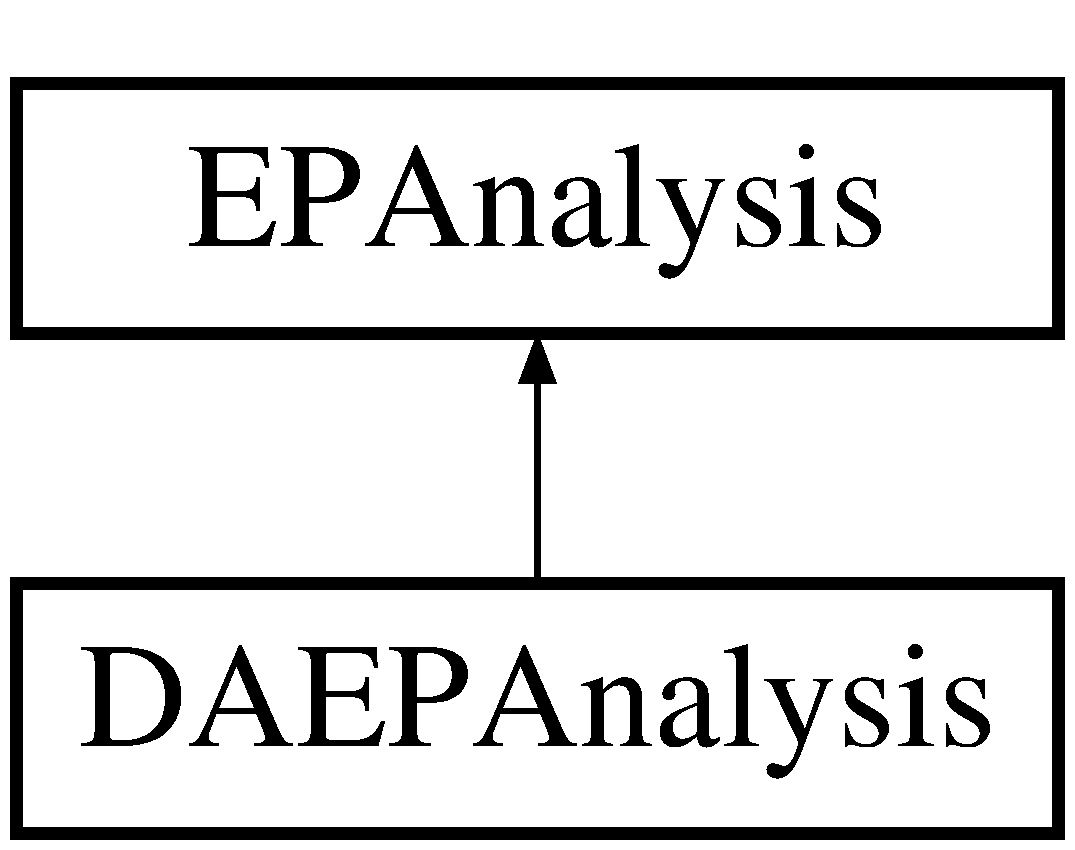
\includegraphics[height=2.000000cm]{class_d_a_e_p_analysis}
\end{center}
\end{figure}
\subsection*{Public Member Functions}
\begin{DoxyCompactItemize}
\item 
\hyperlink{class_d_a_e_p_analysis_a543fae6145bccbf58f2930501fc76f05}{D\+A\+E\+P\+Analysis} ()
\item 
\hyperlink{class_d_a_e_p_analysis_a422717d446880c140110d51610c0c571}{$\sim$\+D\+A\+E\+P\+Analysis} ()
\end{DoxyCompactItemize}
\subsection*{Protected Member Functions}
\begin{DoxyCompactItemize}
\item 
virtual void \hyperlink{class_d_a_e_p_analysis_af2b91e8bd16a65ec962b748bbf27952a}{calc\+One\+Block\+Background} (int index)
\item 
virtual void \hyperlink{class_d_a_e_p_analysis_ae9996fd139ffd800e5a5be4315b50942}{calc\+One\+Block\+Speech} (int index)
\end{DoxyCompactItemize}
\subsection*{Additional Inherited Members}


\subsection{Constructor \& Destructor Documentation}
\hypertarget{class_d_a_e_p_analysis_a543fae6145bccbf58f2930501fc76f05}{\index{D\+A\+E\+P\+Analysis@{D\+A\+E\+P\+Analysis}!D\+A\+E\+P\+Analysis@{D\+A\+E\+P\+Analysis}}
\index{D\+A\+E\+P\+Analysis@{D\+A\+E\+P\+Analysis}!D\+A\+E\+P\+Analysis@{D\+A\+E\+P\+Analysis}}
\subsubsection[{D\+A\+E\+P\+Analysis}]{\setlength{\rightskip}{0pt plus 5cm}D\+A\+E\+P\+Analysis\+::\+D\+A\+E\+P\+Analysis (
\begin{DoxyParamCaption}
{}
\end{DoxyParamCaption}
)\hspace{0.3cm}{\ttfamily [inline]}}}\label{class_d_a_e_p_analysis_a543fae6145bccbf58f2930501fc76f05}
\hypertarget{class_d_a_e_p_analysis_a422717d446880c140110d51610c0c571}{\index{D\+A\+E\+P\+Analysis@{D\+A\+E\+P\+Analysis}!````~D\+A\+E\+P\+Analysis@{$\sim$\+D\+A\+E\+P\+Analysis}}
\index{````~D\+A\+E\+P\+Analysis@{$\sim$\+D\+A\+E\+P\+Analysis}!D\+A\+E\+P\+Analysis@{D\+A\+E\+P\+Analysis}}
\subsubsection[{$\sim$\+D\+A\+E\+P\+Analysis}]{\setlength{\rightskip}{0pt plus 5cm}D\+A\+E\+P\+Analysis\+::$\sim$\+D\+A\+E\+P\+Analysis (
\begin{DoxyParamCaption}
{}
\end{DoxyParamCaption}
)\hspace{0.3cm}{\ttfamily [inline]}}}\label{class_d_a_e_p_analysis_a422717d446880c140110d51610c0c571}


\subsection{Member Function Documentation}
\hypertarget{class_d_a_e_p_analysis_af2b91e8bd16a65ec962b748bbf27952a}{\index{D\+A\+E\+P\+Analysis@{D\+A\+E\+P\+Analysis}!calc\+One\+Block\+Background@{calc\+One\+Block\+Background}}
\index{calc\+One\+Block\+Background@{calc\+One\+Block\+Background}!D\+A\+E\+P\+Analysis@{D\+A\+E\+P\+Analysis}}
\subsubsection[{calc\+One\+Block\+Background}]{\setlength{\rightskip}{0pt plus 5cm}void D\+A\+E\+P\+Analysis\+::calc\+One\+Block\+Background (
\begin{DoxyParamCaption}
\item[{int}]{index}
\end{DoxyParamCaption}
)\hspace{0.3cm}{\ttfamily [protected]}, {\ttfamily [virtual]}}}\label{class_d_a_e_p_analysis_af2b91e8bd16a65ec962b748bbf27952a}


Implements \hyperlink{class_e_p_analysis_ac0d297dde8d0e9663f2e2e3b5fa0bc39}{E\+P\+Analysis}.

\hypertarget{class_d_a_e_p_analysis_ae9996fd139ffd800e5a5be4315b50942}{\index{D\+A\+E\+P\+Analysis@{D\+A\+E\+P\+Analysis}!calc\+One\+Block\+Speech@{calc\+One\+Block\+Speech}}
\index{calc\+One\+Block\+Speech@{calc\+One\+Block\+Speech}!D\+A\+E\+P\+Analysis@{D\+A\+E\+P\+Analysis}}
\subsubsection[{calc\+One\+Block\+Speech}]{\setlength{\rightskip}{0pt plus 5cm}void D\+A\+E\+P\+Analysis\+::calc\+One\+Block\+Speech (
\begin{DoxyParamCaption}
\item[{int}]{index}
\end{DoxyParamCaption}
)\hspace{0.3cm}{\ttfamily [protected]}, {\ttfamily [virtual]}}}\label{class_d_a_e_p_analysis_ae9996fd139ffd800e5a5be4315b50942}


Implements \hyperlink{class_e_p_analysis_a7767c0329b482231ec33faf935a620ce}{E\+P\+Analysis}.



The documentation for this class was generated from the following files\+:\begin{DoxyCompactItemize}
\item 
src/\+Analysis/\hyperlink{_d_a_e_p_analysis_8h}{D\+A\+E\+P\+Analysis.\+h}\item 
src/\+Analysis/\hyperlink{_d_a_e_p_analysis_8cpp}{D\+A\+E\+P\+Analysis.\+cpp}\end{DoxyCompactItemize}

\hypertarget{struct_dtw___column___link}{\section{Dtw\+\_\+\+Column\+\_\+\+Link Struct Reference}
\label{struct_dtw___column___link}\index{Dtw\+\_\+\+Column\+\_\+\+Link@{Dtw\+\_\+\+Column\+\_\+\+Link}}
}


{\ttfamily \#include $<$Seq\+Model.\+h$>$}

\subsection*{Public Member Functions}
\begin{DoxyCompactItemize}
\item 
void \hyperlink{struct_dtw___column___link_a17058f5a2ac47f17c50df04b1f7cb4c7}{add\+Column\+Node} (int node)
\item 
void \hyperlink{struct_dtw___column___link_a1ab71685f6ba7da0607564f000f97ab6}{clear} ()
\end{DoxyCompactItemize}
\subsection*{Public Attributes}
\begin{DoxyCompactItemize}
\item 
int \hyperlink{struct_dtw___column___link_ab80f07bc3099877bfa99c9acbcad194c}{head}
\item 
\hyperlink{struct_dtw___column___node}{Dtw\+\_\+\+Column\+\_\+\+Node} $\ast$ \hyperlink{struct_dtw___column___link_a8c41027581a5dd1cb17341b712680453}{nodes}
\end{DoxyCompactItemize}


\subsection{Member Function Documentation}
\hypertarget{struct_dtw___column___link_a17058f5a2ac47f17c50df04b1f7cb4c7}{\index{Dtw\+\_\+\+Column\+\_\+\+Link@{Dtw\+\_\+\+Column\+\_\+\+Link}!add\+Column\+Node@{add\+Column\+Node}}
\index{add\+Column\+Node@{add\+Column\+Node}!Dtw\+\_\+\+Column\+\_\+\+Link@{Dtw\+\_\+\+Column\+\_\+\+Link}}
\subsubsection[{add\+Column\+Node}]{\setlength{\rightskip}{0pt plus 5cm}void Dtw\+\_\+\+Column\+\_\+\+Link\+::add\+Column\+Node (
\begin{DoxyParamCaption}
\item[{int}]{node}
\end{DoxyParamCaption}
)\hspace{0.3cm}{\ttfamily [inline]}}}\label{struct_dtw___column___link_a17058f5a2ac47f17c50df04b1f7cb4c7}
\hypertarget{struct_dtw___column___link_a1ab71685f6ba7da0607564f000f97ab6}{\index{Dtw\+\_\+\+Column\+\_\+\+Link@{Dtw\+\_\+\+Column\+\_\+\+Link}!clear@{clear}}
\index{clear@{clear}!Dtw\+\_\+\+Column\+\_\+\+Link@{Dtw\+\_\+\+Column\+\_\+\+Link}}
\subsubsection[{clear}]{\setlength{\rightskip}{0pt plus 5cm}void Dtw\+\_\+\+Column\+\_\+\+Link\+::clear (
\begin{DoxyParamCaption}
{}
\end{DoxyParamCaption}
)\hspace{0.3cm}{\ttfamily [inline]}}}\label{struct_dtw___column___link_a1ab71685f6ba7da0607564f000f97ab6}


\subsection{Member Data Documentation}
\hypertarget{struct_dtw___column___link_ab80f07bc3099877bfa99c9acbcad194c}{\index{Dtw\+\_\+\+Column\+\_\+\+Link@{Dtw\+\_\+\+Column\+\_\+\+Link}!head@{head}}
\index{head@{head}!Dtw\+\_\+\+Column\+\_\+\+Link@{Dtw\+\_\+\+Column\+\_\+\+Link}}
\subsubsection[{head}]{\setlength{\rightskip}{0pt plus 5cm}int Dtw\+\_\+\+Column\+\_\+\+Link\+::head}}\label{struct_dtw___column___link_ab80f07bc3099877bfa99c9acbcad194c}
\hypertarget{struct_dtw___column___link_a8c41027581a5dd1cb17341b712680453}{\index{Dtw\+\_\+\+Column\+\_\+\+Link@{Dtw\+\_\+\+Column\+\_\+\+Link}!nodes@{nodes}}
\index{nodes@{nodes}!Dtw\+\_\+\+Column\+\_\+\+Link@{Dtw\+\_\+\+Column\+\_\+\+Link}}
\subsubsection[{nodes}]{\setlength{\rightskip}{0pt plus 5cm}{\bf Dtw\+\_\+\+Column\+\_\+\+Node}$\ast$ Dtw\+\_\+\+Column\+\_\+\+Link\+::nodes}}\label{struct_dtw___column___link_a8c41027581a5dd1cb17341b712680453}


The documentation for this struct was generated from the following file\+:\begin{DoxyCompactItemize}
\item 
src/\+Feature/\hyperlink{_seq_model_8h}{Seq\+Model.\+h}\end{DoxyCompactItemize}

\hypertarget{struct_dtw___column___node}{\section{Dtw\+\_\+\+Column\+\_\+\+Node Struct Reference}
\label{struct_dtw___column___node}\index{Dtw\+\_\+\+Column\+\_\+\+Node@{Dtw\+\_\+\+Column\+\_\+\+Node}}
}


{\ttfamily \#include $<$Seq\+Model.\+h$>$}

\subsection*{Public Member Functions}
\begin{DoxyCompactItemize}
\item 
\hyperlink{struct_dtw___column___node_a7f5eaa822de02a86ddcac32b20e0b0c1}{Dtw\+\_\+\+Column\+\_\+\+Node} ()
\end{DoxyCompactItemize}
\subsection*{Public Attributes}
\begin{DoxyCompactItemize}
\item 
int \hyperlink{struct_dtw___column___node_ae39557fcb83f68ccb31dce3d265c17e0}{pre\+Idx}
\item 
double \hyperlink{struct_dtw___column___node_a4da0707e24783e6dac4af2df75089ad8}{cost}
\item 
int \hyperlink{struct_dtw___column___node_a820a6ed2870d932e2f371bc66bb9ba84}{last\+Update}
\item 
int \hyperlink{struct_dtw___column___node_affe8cf80f0a27940aea2ed5e2cf5b7a0}{next}
\end{DoxyCompactItemize}


\subsection{Constructor \& Destructor Documentation}
\hypertarget{struct_dtw___column___node_a7f5eaa822de02a86ddcac32b20e0b0c1}{\index{Dtw\+\_\+\+Column\+\_\+\+Node@{Dtw\+\_\+\+Column\+\_\+\+Node}!Dtw\+\_\+\+Column\+\_\+\+Node@{Dtw\+\_\+\+Column\+\_\+\+Node}}
\index{Dtw\+\_\+\+Column\+\_\+\+Node@{Dtw\+\_\+\+Column\+\_\+\+Node}!Dtw\+\_\+\+Column\+\_\+\+Node@{Dtw\+\_\+\+Column\+\_\+\+Node}}
\subsubsection[{Dtw\+\_\+\+Column\+\_\+\+Node}]{\setlength{\rightskip}{0pt plus 5cm}Dtw\+\_\+\+Column\+\_\+\+Node\+::\+Dtw\+\_\+\+Column\+\_\+\+Node (
\begin{DoxyParamCaption}
{}
\end{DoxyParamCaption}
)\hspace{0.3cm}{\ttfamily [inline]}}}\label{struct_dtw___column___node_a7f5eaa822de02a86ddcac32b20e0b0c1}


\subsection{Member Data Documentation}
\hypertarget{struct_dtw___column___node_a4da0707e24783e6dac4af2df75089ad8}{\index{Dtw\+\_\+\+Column\+\_\+\+Node@{Dtw\+\_\+\+Column\+\_\+\+Node}!cost@{cost}}
\index{cost@{cost}!Dtw\+\_\+\+Column\+\_\+\+Node@{Dtw\+\_\+\+Column\+\_\+\+Node}}
\subsubsection[{cost}]{\setlength{\rightskip}{0pt plus 5cm}double Dtw\+\_\+\+Column\+\_\+\+Node\+::cost}}\label{struct_dtw___column___node_a4da0707e24783e6dac4af2df75089ad8}
\hypertarget{struct_dtw___column___node_a820a6ed2870d932e2f371bc66bb9ba84}{\index{Dtw\+\_\+\+Column\+\_\+\+Node@{Dtw\+\_\+\+Column\+\_\+\+Node}!last\+Update@{last\+Update}}
\index{last\+Update@{last\+Update}!Dtw\+\_\+\+Column\+\_\+\+Node@{Dtw\+\_\+\+Column\+\_\+\+Node}}
\subsubsection[{last\+Update}]{\setlength{\rightskip}{0pt plus 5cm}int Dtw\+\_\+\+Column\+\_\+\+Node\+::last\+Update}}\label{struct_dtw___column___node_a820a6ed2870d932e2f371bc66bb9ba84}
\hypertarget{struct_dtw___column___node_affe8cf80f0a27940aea2ed5e2cf5b7a0}{\index{Dtw\+\_\+\+Column\+\_\+\+Node@{Dtw\+\_\+\+Column\+\_\+\+Node}!next@{next}}
\index{next@{next}!Dtw\+\_\+\+Column\+\_\+\+Node@{Dtw\+\_\+\+Column\+\_\+\+Node}}
\subsubsection[{next}]{\setlength{\rightskip}{0pt plus 5cm}int Dtw\+\_\+\+Column\+\_\+\+Node\+::next}}\label{struct_dtw___column___node_affe8cf80f0a27940aea2ed5e2cf5b7a0}
\hypertarget{struct_dtw___column___node_ae39557fcb83f68ccb31dce3d265c17e0}{\index{Dtw\+\_\+\+Column\+\_\+\+Node@{Dtw\+\_\+\+Column\+\_\+\+Node}!pre\+Idx@{pre\+Idx}}
\index{pre\+Idx@{pre\+Idx}!Dtw\+\_\+\+Column\+\_\+\+Node@{Dtw\+\_\+\+Column\+\_\+\+Node}}
\subsubsection[{pre\+Idx}]{\setlength{\rightskip}{0pt plus 5cm}int Dtw\+\_\+\+Column\+\_\+\+Node\+::pre\+Idx}}\label{struct_dtw___column___node_ae39557fcb83f68ccb31dce3d265c17e0}


The documentation for this struct was generated from the following file\+:\begin{DoxyCompactItemize}
\item 
src/\+Feature/\hyperlink{_seq_model_8h}{Seq\+Model.\+h}\end{DoxyCompactItemize}

\hypertarget{class_dummy_state}{\section{Dummy\+State Class Reference}
\label{class_dummy_state}\index{Dummy\+State@{Dummy\+State}}
}


{\ttfamily \#include $<$Dummy\+State.\+h$>$}

Inheritance diagram for Dummy\+State\+:\begin{figure}[H]
\begin{center}
\leavevmode
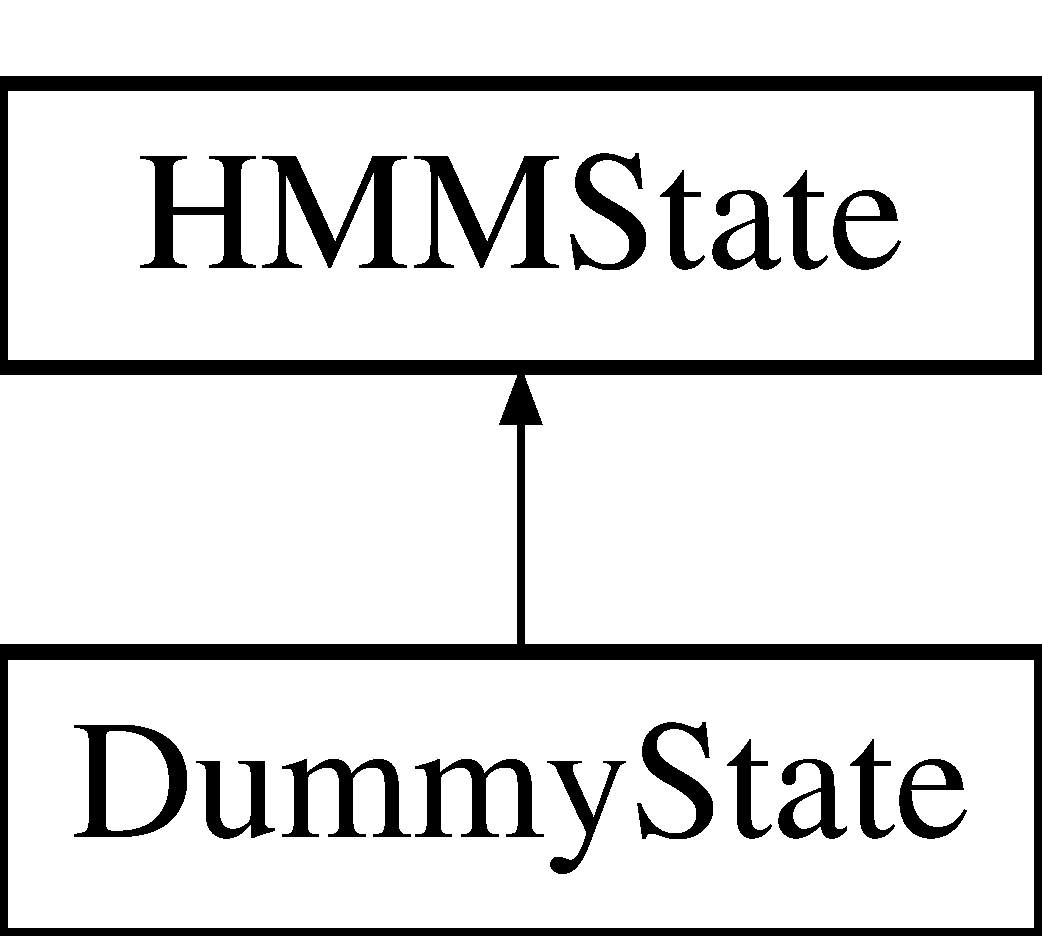
\includegraphics[height=2.000000cm]{class_dummy_state}
\end{center}
\end{figure}
\subsection*{Public Member Functions}
\begin{DoxyCompactItemize}
\item 
\hyperlink{class_dummy_state_a968f19f362de62f9cabad8a110909d00}{Dummy\+State} (std\+::vector$<$ \hyperlink{class_wave_feature_o_p}{Wave\+Feature\+O\+P} $>$ $\ast$\hyperlink{class_h_m_m_state_a04d0b1a1570a339e5cd0db13aeb0d2ae}{templates})
\item 
\hyperlink{class_dummy_state_a21d9845c645182e4899d92ac63e042b0}{$\sim$\+Dummy\+State} ()
\item 
void \hyperlink{class_dummy_state_a3ea8e5a558e56079610eb1b0faee2ef9}{gaussian\+Train} (int gaussian\+Num)
\item 
double \hyperlink{class_dummy_state_a696495e250c01d42c48c6a5f79b1f1d8}{node\+Cost} (\hyperlink{class_feature}{Feature} $\ast$input\+Feature)
\item 
void \hyperlink{class_dummy_state_a7aecab0455227d309908efd3c0cdbaa3}{load} (std\+::stringstream \&in, int \&\hyperlink{pro6__demo_8cpp_a923ffcfa3c56ccdba17bc4e700247d54}{gauss\+Num})
\item 
void \hyperlink{class_dummy_state_a3759cade768196f1f920aa683336ed55}{store} (std\+::stringstream \&out)
\end{DoxyCompactItemize}
\subsection*{Additional Inherited Members}


\subsection{Constructor \& Destructor Documentation}
\hypertarget{class_dummy_state_a968f19f362de62f9cabad8a110909d00}{\index{Dummy\+State@{Dummy\+State}!Dummy\+State@{Dummy\+State}}
\index{Dummy\+State@{Dummy\+State}!Dummy\+State@{Dummy\+State}}
\subsubsection[{Dummy\+State}]{\setlength{\rightskip}{0pt plus 5cm}Dummy\+State\+::\+Dummy\+State (
\begin{DoxyParamCaption}
\item[{std\+::vector$<$ {\bf Wave\+Feature\+O\+P} $>$ $\ast$}]{templates}
\end{DoxyParamCaption}
)\hspace{0.3cm}{\ttfamily [inline]}}}\label{class_dummy_state_a968f19f362de62f9cabad8a110909d00}
\hypertarget{class_dummy_state_a21d9845c645182e4899d92ac63e042b0}{\index{Dummy\+State@{Dummy\+State}!````~Dummy\+State@{$\sim$\+Dummy\+State}}
\index{````~Dummy\+State@{$\sim$\+Dummy\+State}!Dummy\+State@{Dummy\+State}}
\subsubsection[{$\sim$\+Dummy\+State}]{\setlength{\rightskip}{0pt plus 5cm}Dummy\+State\+::$\sim$\+Dummy\+State (
\begin{DoxyParamCaption}
{}
\end{DoxyParamCaption}
)\hspace{0.3cm}{\ttfamily [inline]}}}\label{class_dummy_state_a21d9845c645182e4899d92ac63e042b0}


\subsection{Member Function Documentation}
\hypertarget{class_dummy_state_a3ea8e5a558e56079610eb1b0faee2ef9}{\index{Dummy\+State@{Dummy\+State}!gaussian\+Train@{gaussian\+Train}}
\index{gaussian\+Train@{gaussian\+Train}!Dummy\+State@{Dummy\+State}}
\subsubsection[{gaussian\+Train}]{\setlength{\rightskip}{0pt plus 5cm}void Dummy\+State\+::gaussian\+Train (
\begin{DoxyParamCaption}
\item[{int}]{gaussian\+Num}
\end{DoxyParamCaption}
)\hspace{0.3cm}{\ttfamily [inline]}, {\ttfamily [virtual]}}}\label{class_dummy_state_a3ea8e5a558e56079610eb1b0faee2ef9}


Implements \hyperlink{class_h_m_m_state_a2d42dd972a85014c0f5f9875da1eacd7}{H\+M\+M\+State}.

\hypertarget{class_dummy_state_a7aecab0455227d309908efd3c0cdbaa3}{\index{Dummy\+State@{Dummy\+State}!load@{load}}
\index{load@{load}!Dummy\+State@{Dummy\+State}}
\subsubsection[{load}]{\setlength{\rightskip}{0pt plus 5cm}void Dummy\+State\+::load (
\begin{DoxyParamCaption}
\item[{std\+::stringstream \&}]{in, }
\item[{int \&}]{gauss\+Num}
\end{DoxyParamCaption}
)\hspace{0.3cm}{\ttfamily [inline]}, {\ttfamily [virtual]}}}\label{class_dummy_state_a7aecab0455227d309908efd3c0cdbaa3}


Implements \hyperlink{class_h_m_m_state_ad5d14bf058b8fc39e07319fabebe09ee}{H\+M\+M\+State}.

\hypertarget{class_dummy_state_a696495e250c01d42c48c6a5f79b1f1d8}{\index{Dummy\+State@{Dummy\+State}!node\+Cost@{node\+Cost}}
\index{node\+Cost@{node\+Cost}!Dummy\+State@{Dummy\+State}}
\subsubsection[{node\+Cost}]{\setlength{\rightskip}{0pt plus 5cm}double Dummy\+State\+::node\+Cost (
\begin{DoxyParamCaption}
\item[{{\bf Feature} $\ast$}]{input\+Feature}
\end{DoxyParamCaption}
)\hspace{0.3cm}{\ttfamily [inline]}, {\ttfamily [virtual]}}}\label{class_dummy_state_a696495e250c01d42c48c6a5f79b1f1d8}


Implements \hyperlink{class_h_m_m_state_a84ad1899239f79257837e6d77cc4f242}{H\+M\+M\+State}.

\hypertarget{class_dummy_state_a3759cade768196f1f920aa683336ed55}{\index{Dummy\+State@{Dummy\+State}!store@{store}}
\index{store@{store}!Dummy\+State@{Dummy\+State}}
\subsubsection[{store}]{\setlength{\rightskip}{0pt plus 5cm}void Dummy\+State\+::store (
\begin{DoxyParamCaption}
\item[{std\+::stringstream \&}]{out}
\end{DoxyParamCaption}
)\hspace{0.3cm}{\ttfamily [inline]}, {\ttfamily [virtual]}}}\label{class_dummy_state_a3759cade768196f1f920aa683336ed55}


Implements \hyperlink{class_h_m_m_state_ab12116fc28ade677ee79ff13b4577ea6}{H\+M\+M\+State}.



The documentation for this class was generated from the following file\+:\begin{DoxyCompactItemize}
\item 
src/\+Feature/\hyperlink{_dummy_state_8h}{Dummy\+State.\+h}\end{DoxyCompactItemize}

\hypertarget{class_e_p_analysis}{\section{E\+P\+Analysis Class Reference}
\label{class_e_p_analysis}\index{E\+P\+Analysis@{E\+P\+Analysis}}
}


{\ttfamily \#include $<$E\+P\+Analysis.\+h$>$}

Inheritance diagram for E\+P\+Analysis\+:\begin{figure}[H]
\begin{center}
\leavevmode
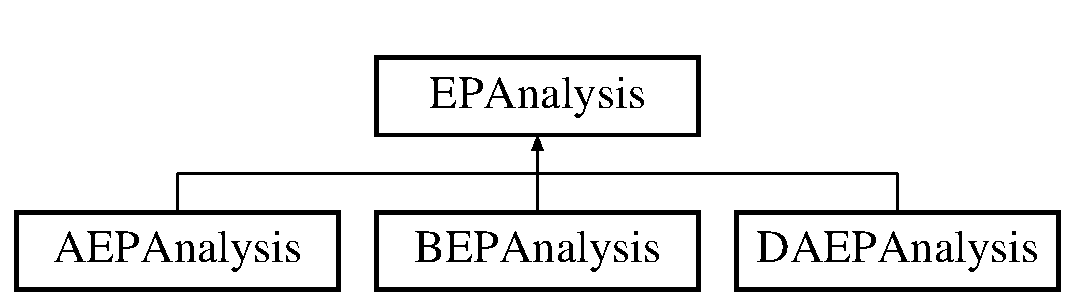
\includegraphics[height=2.000000cm]{class_e_p_analysis}
\end{center}
\end{figure}
\subsection*{Public Member Functions}
\begin{DoxyCompactItemize}
\item 
\hyperlink{class_e_p_analysis_a0b65e06f79424966ef106c1f39cdc2dc}{E\+P\+Analysis} ()
\item 
\hyperlink{class_e_p_analysis_a0bf9e48c6441fed0f5d7c8e755f097f3}{$\sim$\+E\+P\+Analysis} ()
\item 
\hyperlink{class_raw_data}{Raw\+Data} $\ast$ \hyperlink{class_e_p_analysis_a09d2b16c0ff0e77fc66c74e54ee1c279}{data} ()
\item 
virtual void \hyperlink{class_e_p_analysis_a7e7311c513772986b89d97c7bde0eb39}{Initial} (\hyperlink{class_raw_data}{Raw\+Data} $\ast$raw\+Data)
\item 
bool \hyperlink{class_e_p_analysis_a5689e3c5824f3640bc76affd01d5724e}{add\+One\+Block\+Data\+With\+End\+Flag} (const \hyperlink{configure__basic_8h_abf32ffaff24ba21700fbd0898b49ab02}{S\+O\+U\+N\+D\+\_\+\+D\+A\+T\+A} $\ast$src)
\item 
void \hyperlink{class_e_p_analysis_a957fbafe0e4a9f7080ea4c37bcbd212c}{re\+Calc\+All\+Data} ()
\item 
void \hyperlink{class_e_p_analysis_a295580a18959d01e9f87a7514c5a0e74}{smooth} ()
\item 
void \hyperlink{class_e_p_analysis_a4b999949ec5b73194b29a533da8f00c8}{cut} ()
\item 
virtual int \hyperlink{class_e_p_analysis_a04fb7764261d7d579aa5bc98331b8a16}{print\+Inf} (int from, int \hyperlink{lpc2spec_8m_a75a3ccc1a712583b6c4b21b94514a7b9}{end}=-\/1)
\item 
virtual bool \hyperlink{class_e_p_analysis_a082819267ab6a37c293a07cf5e3e792b}{save\+Matlab} (const char $\ast$file\+\_\+name)
\end{DoxyCompactItemize}
\subsection*{Protected Member Functions}
\begin{DoxyCompactItemize}
\item 
\hyperlink{class_e_p_analysis_ad1d552418bdac23493701f726303c088}{R\+E\+A\+D\+\_\+\+W\+R\+I\+T\+E\+\_\+\+D\+E\+C\+L\+A\+R\+E} (\hyperlink{class_raw_data}{Raw\+Data} $\ast$, raw\+Data, \hyperlink{class_raw_data}{Raw\+Data})
\item 
virtual void \hyperlink{class_e_p_analysis_acd38ed7c170e41ce73a2af3f1e8b442f}{calc\+One\+Block\+Energe} (int index)
\item 
virtual void \hyperlink{class_e_p_analysis_ac0d297dde8d0e9663f2e2e3b5fa0bc39}{calc\+One\+Block\+Background} (int index)=0
\item 
virtual void \hyperlink{class_e_p_analysis_a7767c0329b482231ec33faf935a620ce}{calc\+One\+Block\+Speech} (int index)=0
\item 
virtual void \hyperlink{class_e_p_analysis_aba99bc553c0e1f82ca844a5130263e6f}{calc\+One\+Block\+Other\+Data} (int index)
\item 
void \hyperlink{class_e_p_analysis_a8390360185d73e872b00c1207ea3cd55}{calc\+One\+Block\+Data} (int index)
\item 
bool \hyperlink{class_e_p_analysis_a4bfa7381a0d922990521779f6c4b3ce5}{append\+One\+Block\+Data} (const \hyperlink{configure__basic_8h_abf32ffaff24ba21700fbd0898b49ab02}{S\+O\+U\+N\+D\+\_\+\+D\+A\+T\+A} $\ast$src)
\item 
virtual bool \hyperlink{class_e_p_analysis_aa9964f5d1dd52e46156ff2304104d26d}{check\+Continue} ()
\item 
virtual void \hyperlink{class_e_p_analysis_a0c4270a435264c7aa18408d7f350ca31}{save\+Other\+Data} (F\+I\+L\+E $\ast$\hyperlink{readhtk_8m_ae135fff58330ebb77574e0dd6280aa68}{fid})
\item 
void \hyperlink{class_e_p_analysis_a195f5fff329e1df4862758baa80a9454}{change\+Silent\+Segment\+Into\+Speech} ()
\item 
void \hyperlink{class_e_p_analysis_aeca6d7b752d925d884bee17237007bb4}{change\+Speech\+Segment\+Into\+Silent} ()
\end{DoxyCompactItemize}
\subsection*{Protected Attributes}
\begin{DoxyCompactItemize}
\item 
int \hyperlink{class_e_p_analysis_ab9ee2c7ec0c37fd120489f625ad64cde}{block\+\_\+num}
\item 
int \hyperlink{class_e_p_analysis_a16dfd308b2c4ba9cfc63be3b8867da6a}{silent\+Time}
\item 
vector$<$ double $>$ \hyperlink{class_e_p_analysis_a08a51e10aeea685b4ae0980b694c396a}{background}
\item 
vector$<$ double $>$ \hyperlink{class_e_p_analysis_a16d60a56e47c6fd90658dd564badfad3}{energy}
\item 
vector$<$ char $>$ \hyperlink{class_e_p_analysis_a349b8500c98d922a49610f2c801ab7ec}{speech}
\end{DoxyCompactItemize}


\subsection{Constructor \& Destructor Documentation}
\hypertarget{class_e_p_analysis_a0b65e06f79424966ef106c1f39cdc2dc}{\index{E\+P\+Analysis@{E\+P\+Analysis}!E\+P\+Analysis@{E\+P\+Analysis}}
\index{E\+P\+Analysis@{E\+P\+Analysis}!E\+P\+Analysis@{E\+P\+Analysis}}
\subsubsection[{E\+P\+Analysis}]{\setlength{\rightskip}{0pt plus 5cm}E\+P\+Analysis\+::\+E\+P\+Analysis (
\begin{DoxyParamCaption}
{}
\end{DoxyParamCaption}
)\hspace{0.3cm}{\ttfamily [inline]}}}\label{class_e_p_analysis_a0b65e06f79424966ef106c1f39cdc2dc}
\hypertarget{class_e_p_analysis_a0bf9e48c6441fed0f5d7c8e755f097f3}{\index{E\+P\+Analysis@{E\+P\+Analysis}!````~E\+P\+Analysis@{$\sim$\+E\+P\+Analysis}}
\index{````~E\+P\+Analysis@{$\sim$\+E\+P\+Analysis}!E\+P\+Analysis@{E\+P\+Analysis}}
\subsubsection[{$\sim$\+E\+P\+Analysis}]{\setlength{\rightskip}{0pt plus 5cm}E\+P\+Analysis\+::$\sim$\+E\+P\+Analysis (
\begin{DoxyParamCaption}
{}
\end{DoxyParamCaption}
)\hspace{0.3cm}{\ttfamily [inline]}}}\label{class_e_p_analysis_a0bf9e48c6441fed0f5d7c8e755f097f3}


\subsection{Member Function Documentation}
\hypertarget{class_e_p_analysis_a5689e3c5824f3640bc76affd01d5724e}{\index{E\+P\+Analysis@{E\+P\+Analysis}!add\+One\+Block\+Data\+With\+End\+Flag@{add\+One\+Block\+Data\+With\+End\+Flag}}
\index{add\+One\+Block\+Data\+With\+End\+Flag@{add\+One\+Block\+Data\+With\+End\+Flag}!E\+P\+Analysis@{E\+P\+Analysis}}
\subsubsection[{add\+One\+Block\+Data\+With\+End\+Flag}]{\setlength{\rightskip}{0pt plus 5cm}bool E\+P\+Analysis\+::add\+One\+Block\+Data\+With\+End\+Flag (
\begin{DoxyParamCaption}
\item[{const {\bf S\+O\+U\+N\+D\+\_\+\+D\+A\+T\+A} $\ast$}]{src}
\end{DoxyParamCaption}
)}}\label{class_e_p_analysis_a5689e3c5824f3640bc76affd01d5724e}
\hypertarget{class_e_p_analysis_a4bfa7381a0d922990521779f6c4b3ce5}{\index{E\+P\+Analysis@{E\+P\+Analysis}!append\+One\+Block\+Data@{append\+One\+Block\+Data}}
\index{append\+One\+Block\+Data@{append\+One\+Block\+Data}!E\+P\+Analysis@{E\+P\+Analysis}}
\subsubsection[{append\+One\+Block\+Data}]{\setlength{\rightskip}{0pt plus 5cm}bool E\+P\+Analysis\+::append\+One\+Block\+Data (
\begin{DoxyParamCaption}
\item[{const {\bf S\+O\+U\+N\+D\+\_\+\+D\+A\+T\+A} $\ast$}]{src}
\end{DoxyParamCaption}
)\hspace{0.3cm}{\ttfamily [protected]}}}\label{class_e_p_analysis_a4bfa7381a0d922990521779f6c4b3ce5}
\hypertarget{class_e_p_analysis_ac0d297dde8d0e9663f2e2e3b5fa0bc39}{\index{E\+P\+Analysis@{E\+P\+Analysis}!calc\+One\+Block\+Background@{calc\+One\+Block\+Background}}
\index{calc\+One\+Block\+Background@{calc\+One\+Block\+Background}!E\+P\+Analysis@{E\+P\+Analysis}}
\subsubsection[{calc\+One\+Block\+Background}]{\setlength{\rightskip}{0pt plus 5cm}virtual void E\+P\+Analysis\+::calc\+One\+Block\+Background (
\begin{DoxyParamCaption}
\item[{int}]{index}
\end{DoxyParamCaption}
)\hspace{0.3cm}{\ttfamily [protected]}, {\ttfamily [pure virtual]}}}\label{class_e_p_analysis_ac0d297dde8d0e9663f2e2e3b5fa0bc39}


Implemented in \hyperlink{class_a_e_p_analysis_abdec61d75b30f2d6753c3c237e2b6805}{A\+E\+P\+Analysis}, \hyperlink{class_b_e_p_analysis_ace11d41c17bd9fbbbdddb85ccccb070e}{B\+E\+P\+Analysis}, and \hyperlink{class_d_a_e_p_analysis_af2b91e8bd16a65ec962b748bbf27952a}{D\+A\+E\+P\+Analysis}.

\hypertarget{class_e_p_analysis_a8390360185d73e872b00c1207ea3cd55}{\index{E\+P\+Analysis@{E\+P\+Analysis}!calc\+One\+Block\+Data@{calc\+One\+Block\+Data}}
\index{calc\+One\+Block\+Data@{calc\+One\+Block\+Data}!E\+P\+Analysis@{E\+P\+Analysis}}
\subsubsection[{calc\+One\+Block\+Data}]{\setlength{\rightskip}{0pt plus 5cm}void E\+P\+Analysis\+::calc\+One\+Block\+Data (
\begin{DoxyParamCaption}
\item[{int}]{index}
\end{DoxyParamCaption}
)\hspace{0.3cm}{\ttfamily [protected]}}}\label{class_e_p_analysis_a8390360185d73e872b00c1207ea3cd55}
\hypertarget{class_e_p_analysis_acd38ed7c170e41ce73a2af3f1e8b442f}{\index{E\+P\+Analysis@{E\+P\+Analysis}!calc\+One\+Block\+Energe@{calc\+One\+Block\+Energe}}
\index{calc\+One\+Block\+Energe@{calc\+One\+Block\+Energe}!E\+P\+Analysis@{E\+P\+Analysis}}
\subsubsection[{calc\+One\+Block\+Energe}]{\setlength{\rightskip}{0pt plus 5cm}void E\+P\+Analysis\+::calc\+One\+Block\+Energe (
\begin{DoxyParamCaption}
\item[{int}]{index}
\end{DoxyParamCaption}
)\hspace{0.3cm}{\ttfamily [protected]}, {\ttfamily [virtual]}}}\label{class_e_p_analysis_acd38ed7c170e41ce73a2af3f1e8b442f}
\hypertarget{class_e_p_analysis_aba99bc553c0e1f82ca844a5130263e6f}{\index{E\+P\+Analysis@{E\+P\+Analysis}!calc\+One\+Block\+Other\+Data@{calc\+One\+Block\+Other\+Data}}
\index{calc\+One\+Block\+Other\+Data@{calc\+One\+Block\+Other\+Data}!E\+P\+Analysis@{E\+P\+Analysis}}
\subsubsection[{calc\+One\+Block\+Other\+Data}]{\setlength{\rightskip}{0pt plus 5cm}virtual void E\+P\+Analysis\+::calc\+One\+Block\+Other\+Data (
\begin{DoxyParamCaption}
\item[{int}]{index}
\end{DoxyParamCaption}
)\hspace{0.3cm}{\ttfamily [inline]}, {\ttfamily [protected]}, {\ttfamily [virtual]}}}\label{class_e_p_analysis_aba99bc553c0e1f82ca844a5130263e6f}


Reimplemented in \hyperlink{class_a_e_p_analysis_a270d364445bb9ed0d82f2bc15791c046}{A\+E\+P\+Analysis}.

\hypertarget{class_e_p_analysis_a7767c0329b482231ec33faf935a620ce}{\index{E\+P\+Analysis@{E\+P\+Analysis}!calc\+One\+Block\+Speech@{calc\+One\+Block\+Speech}}
\index{calc\+One\+Block\+Speech@{calc\+One\+Block\+Speech}!E\+P\+Analysis@{E\+P\+Analysis}}
\subsubsection[{calc\+One\+Block\+Speech}]{\setlength{\rightskip}{0pt plus 5cm}virtual void E\+P\+Analysis\+::calc\+One\+Block\+Speech (
\begin{DoxyParamCaption}
\item[{int}]{index}
\end{DoxyParamCaption}
)\hspace{0.3cm}{\ttfamily [protected]}, {\ttfamily [pure virtual]}}}\label{class_e_p_analysis_a7767c0329b482231ec33faf935a620ce}


Implemented in \hyperlink{class_a_e_p_analysis_a367b638a878435cf86de9b4b384b61a0}{A\+E\+P\+Analysis}, \hyperlink{class_b_e_p_analysis_ab508a682d38fbc58319ea48bfaa54615}{B\+E\+P\+Analysis}, and \hyperlink{class_d_a_e_p_analysis_ae9996fd139ffd800e5a5be4315b50942}{D\+A\+E\+P\+Analysis}.

\hypertarget{class_e_p_analysis_a195f5fff329e1df4862758baa80a9454}{\index{E\+P\+Analysis@{E\+P\+Analysis}!change\+Silent\+Segment\+Into\+Speech@{change\+Silent\+Segment\+Into\+Speech}}
\index{change\+Silent\+Segment\+Into\+Speech@{change\+Silent\+Segment\+Into\+Speech}!E\+P\+Analysis@{E\+P\+Analysis}}
\subsubsection[{change\+Silent\+Segment\+Into\+Speech}]{\setlength{\rightskip}{0pt plus 5cm}void E\+P\+Analysis\+::change\+Silent\+Segment\+Into\+Speech (
\begin{DoxyParamCaption}
{}
\end{DoxyParamCaption}
)\hspace{0.3cm}{\ttfamily [protected]}}}\label{class_e_p_analysis_a195f5fff329e1df4862758baa80a9454}
\hypertarget{class_e_p_analysis_aeca6d7b752d925d884bee17237007bb4}{\index{E\+P\+Analysis@{E\+P\+Analysis}!change\+Speech\+Segment\+Into\+Silent@{change\+Speech\+Segment\+Into\+Silent}}
\index{change\+Speech\+Segment\+Into\+Silent@{change\+Speech\+Segment\+Into\+Silent}!E\+P\+Analysis@{E\+P\+Analysis}}
\subsubsection[{change\+Speech\+Segment\+Into\+Silent}]{\setlength{\rightskip}{0pt plus 5cm}void E\+P\+Analysis\+::change\+Speech\+Segment\+Into\+Silent (
\begin{DoxyParamCaption}
{}
\end{DoxyParamCaption}
)\hspace{0.3cm}{\ttfamily [protected]}}}\label{class_e_p_analysis_aeca6d7b752d925d884bee17237007bb4}
\hypertarget{class_e_p_analysis_aa9964f5d1dd52e46156ff2304104d26d}{\index{E\+P\+Analysis@{E\+P\+Analysis}!check\+Continue@{check\+Continue}}
\index{check\+Continue@{check\+Continue}!E\+P\+Analysis@{E\+P\+Analysis}}
\subsubsection[{check\+Continue}]{\setlength{\rightskip}{0pt plus 5cm}bool E\+P\+Analysis\+::check\+Continue (
\begin{DoxyParamCaption}
{}
\end{DoxyParamCaption}
)\hspace{0.3cm}{\ttfamily [protected]}, {\ttfamily [virtual]}}}\label{class_e_p_analysis_aa9964f5d1dd52e46156ff2304104d26d}
\hypertarget{class_e_p_analysis_a4b999949ec5b73194b29a533da8f00c8}{\index{E\+P\+Analysis@{E\+P\+Analysis}!cut@{cut}}
\index{cut@{cut}!E\+P\+Analysis@{E\+P\+Analysis}}
\subsubsection[{cut}]{\setlength{\rightskip}{0pt plus 5cm}void E\+P\+Analysis\+::cut (
\begin{DoxyParamCaption}
{}
\end{DoxyParamCaption}
)}}\label{class_e_p_analysis_a4b999949ec5b73194b29a533da8f00c8}
\hypertarget{class_e_p_analysis_a09d2b16c0ff0e77fc66c74e54ee1c279}{\index{E\+P\+Analysis@{E\+P\+Analysis}!data@{data}}
\index{data@{data}!E\+P\+Analysis@{E\+P\+Analysis}}
\subsubsection[{data}]{\setlength{\rightskip}{0pt plus 5cm}{\bf Raw\+Data}$\ast$ E\+P\+Analysis\+::data (
\begin{DoxyParamCaption}
{}
\end{DoxyParamCaption}
)\hspace{0.3cm}{\ttfamily [inline]}}}\label{class_e_p_analysis_a09d2b16c0ff0e77fc66c74e54ee1c279}
\hypertarget{class_e_p_analysis_a7e7311c513772986b89d97c7bde0eb39}{\index{E\+P\+Analysis@{E\+P\+Analysis}!Initial@{Initial}}
\index{Initial@{Initial}!E\+P\+Analysis@{E\+P\+Analysis}}
\subsubsection[{Initial}]{\setlength{\rightskip}{0pt plus 5cm}virtual void E\+P\+Analysis\+::\+Initial (
\begin{DoxyParamCaption}
\item[{{\bf Raw\+Data} $\ast$}]{raw\+Data}
\end{DoxyParamCaption}
)\hspace{0.3cm}{\ttfamily [inline]}, {\ttfamily [virtual]}}}\label{class_e_p_analysis_a7e7311c513772986b89d97c7bde0eb39}


Reimplemented in \hyperlink{class_a_e_p_analysis_af8c0797c01e6d50d4e3f5e89f98863a3}{A\+E\+P\+Analysis}.

\hypertarget{class_e_p_analysis_a04fb7764261d7d579aa5bc98331b8a16}{\index{E\+P\+Analysis@{E\+P\+Analysis}!print\+Inf@{print\+Inf}}
\index{print\+Inf@{print\+Inf}!E\+P\+Analysis@{E\+P\+Analysis}}
\subsubsection[{print\+Inf}]{\setlength{\rightskip}{0pt plus 5cm}int E\+P\+Analysis\+::print\+Inf (
\begin{DoxyParamCaption}
\item[{int}]{from, }
\item[{int}]{end = {\ttfamily -\/1}}
\end{DoxyParamCaption}
)\hspace{0.3cm}{\ttfamily [virtual]}}}\label{class_e_p_analysis_a04fb7764261d7d579aa5bc98331b8a16}


Reimplemented in \hyperlink{class_a_e_p_analysis_a6349405c9185f6ce4e4d3c5711daa217}{A\+E\+P\+Analysis}.

\hypertarget{class_e_p_analysis_ad1d552418bdac23493701f726303c088}{\index{E\+P\+Analysis@{E\+P\+Analysis}!R\+E\+A\+D\+\_\+\+W\+R\+I\+T\+E\+\_\+\+D\+E\+C\+L\+A\+R\+E@{R\+E\+A\+D\+\_\+\+W\+R\+I\+T\+E\+\_\+\+D\+E\+C\+L\+A\+R\+E}}
\index{R\+E\+A\+D\+\_\+\+W\+R\+I\+T\+E\+\_\+\+D\+E\+C\+L\+A\+R\+E@{R\+E\+A\+D\+\_\+\+W\+R\+I\+T\+E\+\_\+\+D\+E\+C\+L\+A\+R\+E}!E\+P\+Analysis@{E\+P\+Analysis}}
\subsubsection[{R\+E\+A\+D\+\_\+\+W\+R\+I\+T\+E\+\_\+\+D\+E\+C\+L\+A\+R\+E}]{\setlength{\rightskip}{0pt plus 5cm}E\+P\+Analysis\+::\+R\+E\+A\+D\+\_\+\+W\+R\+I\+T\+E\+\_\+\+D\+E\+C\+L\+A\+R\+E (
\begin{DoxyParamCaption}
\item[{{\bf Raw\+Data} $\ast$}]{, }
\item[{raw\+Data}]{, }
\item[{{\bf Raw\+Data}}]{}
\end{DoxyParamCaption}
)\hspace{0.3cm}{\ttfamily [protected]}}}\label{class_e_p_analysis_ad1d552418bdac23493701f726303c088}
\hypertarget{class_e_p_analysis_a957fbafe0e4a9f7080ea4c37bcbd212c}{\index{E\+P\+Analysis@{E\+P\+Analysis}!re\+Calc\+All\+Data@{re\+Calc\+All\+Data}}
\index{re\+Calc\+All\+Data@{re\+Calc\+All\+Data}!E\+P\+Analysis@{E\+P\+Analysis}}
\subsubsection[{re\+Calc\+All\+Data}]{\setlength{\rightskip}{0pt plus 5cm}void E\+P\+Analysis\+::re\+Calc\+All\+Data (
\begin{DoxyParamCaption}
{}
\end{DoxyParamCaption}
)}}\label{class_e_p_analysis_a957fbafe0e4a9f7080ea4c37bcbd212c}
\hypertarget{class_e_p_analysis_a082819267ab6a37c293a07cf5e3e792b}{\index{E\+P\+Analysis@{E\+P\+Analysis}!save\+Matlab@{save\+Matlab}}
\index{save\+Matlab@{save\+Matlab}!E\+P\+Analysis@{E\+P\+Analysis}}
\subsubsection[{save\+Matlab}]{\setlength{\rightskip}{0pt plus 5cm}bool E\+P\+Analysis\+::save\+Matlab (
\begin{DoxyParamCaption}
\item[{const char $\ast$}]{file\+\_\+name}
\end{DoxyParamCaption}
)\hspace{0.3cm}{\ttfamily [virtual]}}}\label{class_e_p_analysis_a082819267ab6a37c293a07cf5e3e792b}
\hypertarget{class_e_p_analysis_a0c4270a435264c7aa18408d7f350ca31}{\index{E\+P\+Analysis@{E\+P\+Analysis}!save\+Other\+Data@{save\+Other\+Data}}
\index{save\+Other\+Data@{save\+Other\+Data}!E\+P\+Analysis@{E\+P\+Analysis}}
\subsubsection[{save\+Other\+Data}]{\setlength{\rightskip}{0pt plus 5cm}virtual void E\+P\+Analysis\+::save\+Other\+Data (
\begin{DoxyParamCaption}
\item[{F\+I\+L\+E $\ast$}]{fid}
\end{DoxyParamCaption}
)\hspace{0.3cm}{\ttfamily [inline]}, {\ttfamily [protected]}, {\ttfamily [virtual]}}}\label{class_e_p_analysis_a0c4270a435264c7aa18408d7f350ca31}


Reimplemented in \hyperlink{class_a_e_p_analysis_a4c230992b22dd17f64614148698a3a17}{A\+E\+P\+Analysis}.

\hypertarget{class_e_p_analysis_a295580a18959d01e9f87a7514c5a0e74}{\index{E\+P\+Analysis@{E\+P\+Analysis}!smooth@{smooth}}
\index{smooth@{smooth}!E\+P\+Analysis@{E\+P\+Analysis}}
\subsubsection[{smooth}]{\setlength{\rightskip}{0pt plus 5cm}void E\+P\+Analysis\+::smooth (
\begin{DoxyParamCaption}
{}
\end{DoxyParamCaption}
)}}\label{class_e_p_analysis_a295580a18959d01e9f87a7514c5a0e74}


\subsection{Member Data Documentation}
\hypertarget{class_e_p_analysis_a08a51e10aeea685b4ae0980b694c396a}{\index{E\+P\+Analysis@{E\+P\+Analysis}!background@{background}}
\index{background@{background}!E\+P\+Analysis@{E\+P\+Analysis}}
\subsubsection[{background}]{\setlength{\rightskip}{0pt plus 5cm}vector$<$double$>$ E\+P\+Analysis\+::background\hspace{0.3cm}{\ttfamily [protected]}}}\label{class_e_p_analysis_a08a51e10aeea685b4ae0980b694c396a}
\hypertarget{class_e_p_analysis_ab9ee2c7ec0c37fd120489f625ad64cde}{\index{E\+P\+Analysis@{E\+P\+Analysis}!block\+\_\+num@{block\+\_\+num}}
\index{block\+\_\+num@{block\+\_\+num}!E\+P\+Analysis@{E\+P\+Analysis}}
\subsubsection[{block\+\_\+num}]{\setlength{\rightskip}{0pt plus 5cm}int E\+P\+Analysis\+::block\+\_\+num\hspace{0.3cm}{\ttfamily [protected]}}}\label{class_e_p_analysis_ab9ee2c7ec0c37fd120489f625ad64cde}
\hypertarget{class_e_p_analysis_a16d60a56e47c6fd90658dd564badfad3}{\index{E\+P\+Analysis@{E\+P\+Analysis}!energy@{energy}}
\index{energy@{energy}!E\+P\+Analysis@{E\+P\+Analysis}}
\subsubsection[{energy}]{\setlength{\rightskip}{0pt plus 5cm}vector$<$double$>$ E\+P\+Analysis\+::energy\hspace{0.3cm}{\ttfamily [protected]}}}\label{class_e_p_analysis_a16d60a56e47c6fd90658dd564badfad3}
\hypertarget{class_e_p_analysis_a16dfd308b2c4ba9cfc63be3b8867da6a}{\index{E\+P\+Analysis@{E\+P\+Analysis}!silent\+Time@{silent\+Time}}
\index{silent\+Time@{silent\+Time}!E\+P\+Analysis@{E\+P\+Analysis}}
\subsubsection[{silent\+Time}]{\setlength{\rightskip}{0pt plus 5cm}int E\+P\+Analysis\+::silent\+Time\hspace{0.3cm}{\ttfamily [protected]}}}\label{class_e_p_analysis_a16dfd308b2c4ba9cfc63be3b8867da6a}
\hypertarget{class_e_p_analysis_a349b8500c98d922a49610f2c801ab7ec}{\index{E\+P\+Analysis@{E\+P\+Analysis}!speech@{speech}}
\index{speech@{speech}!E\+P\+Analysis@{E\+P\+Analysis}}
\subsubsection[{speech}]{\setlength{\rightskip}{0pt plus 5cm}vector$<$char$>$ E\+P\+Analysis\+::speech\hspace{0.3cm}{\ttfamily [protected]}}}\label{class_e_p_analysis_a349b8500c98d922a49610f2c801ab7ec}


The documentation for this class was generated from the following files\+:\begin{DoxyCompactItemize}
\item 
src/\+Analysis/\hyperlink{_e_p_analysis_8h}{E\+P\+Analysis.\+h}\item 
src/\+Analysis/\hyperlink{_e_p_analysis_8cpp}{E\+P\+Analysis.\+cpp}\end{DoxyCompactItemize}

\hypertarget{class_feature}{\section{Feature Class Reference}
\label{class_feature}\index{Feature@{Feature}}
}


{\ttfamily \#include $<$Feature.\+h$>$}

\subsection*{Public Types}
\begin{DoxyCompactItemize}
\item 
enum \hyperlink{class_feature_afa43293b1c8369e9ff47f6eedb7ad264}{Feature\+Type} \{ \hyperlink{class_feature_afa43293b1c8369e9ff47f6eedb7ad264ad1f562be2a0e47fb440219948324ab11}{Raw}, 
\hyperlink{class_feature_afa43293b1c8369e9ff47f6eedb7ad264aff7fd054901faaf35c8d02a3aeefef66}{Delta}, 
\hyperlink{class_feature_afa43293b1c8369e9ff47f6eedb7ad264ac9a34ecf21436bc7a31921d2956b1680}{Double\+Delta}
 \}
\end{DoxyCompactItemize}
\subsection*{Public Member Functions}
\begin{DoxyCompactItemize}
\item 
\hyperlink{class_feature_a06d191f6daea88e0029440a2137f2e07}{Feature} ()
\item 
\hyperlink{class_feature}{Feature} \hyperlink{class_feature_a90f1fbc54bfae85f7edf8234ffbfd29c}{operator$\ast$} (const \hyperlink{class_feature}{Feature} \&T) const 
\item 
\hyperlink{class_feature}{Feature} \hyperlink{class_feature_a7e9d7aa483a2252b914db28edf0c981f}{sqr} ()
\item 
\hyperlink{class_feature}{Feature} \hyperlink{class_feature_a733baf36f22566c35aca39fd29236e0f}{operator+} (const \hyperlink{class_feature}{Feature} \&T) const 
\item 
double \hyperlink{class_feature_a9c94cc178ad282294fa94a795eb0d401}{operator-\/} (const \hyperlink{class_feature}{Feature} \&T)
\item 
\hyperlink{class_feature_afa43293b1c8369e9ff47f6eedb7ad264}{Feature\+Type} \hyperlink{class_feature_a267870d668dfb6c245b00633af6bcb93}{get\+Feature\+Type} ()
\item 
\hyperlink{class_feature_afa43293b1c8369e9ff47f6eedb7ad264}{Feature\+Type} \hyperlink{class_feature_a4ae182413e415b449023c933c9b7f04d}{set\+Feature\+Type} (\hyperlink{class_feature_afa43293b1c8369e9ff47f6eedb7ad264}{Feature\+Type} \hyperlink{class_feature_a9325ce63b0c3062d70ad02a0e51e4ed3}{type})
\item 
\hyperlink{tool_8h_ab71a1f2fb85a32402ced5c483105b38e}{S\+P\+\_\+\+R\+E\+S\+U\+L\+T} \hyperlink{class_feature_a6eb221814384244f007201c41c95f372}{fill\+Delta} ()
\item 
\hyperlink{tool_8h_ab71a1f2fb85a32402ced5c483105b38e}{S\+P\+\_\+\+R\+E\+S\+U\+L\+T} \hyperlink{class_feature_a301410df571143da9c1a584246925122}{fill\+Double\+Delta} ()
\item 
void \hyperlink{class_feature_ab8e0691828f51eddd940bb37c90d7d4f}{push\+\_\+back} (double \hyperlink{deltas_8m_ace9cdca9c1b355d9b321fd7f5ec2026b}{d})
\item 
\hyperlink{class_feature}{Feature} \hyperlink{class_feature_a297dc1375d2e371f1c0ec2cf01d6b9b7}{operator$\ast$} (double \hyperlink{lpc2spec_8m_aa49cfdd4fa4d74d71f78a001a1b635d0}{c}) const 
\item 
void \hyperlink{class_feature_a5f2a277917e11f2b7ae6a3f8a63269b8}{resize} (int s)
\item 
const double \& \hyperlink{class_feature_acd67423c3e4b1ea3ddbd257a5614b728}{operator\mbox{[}$\,$\mbox{]}} (int inx) const 
\item 
double \& \hyperlink{class_feature_abb9d8d94d76d810ff1e27c520635c3d5}{operator\mbox{[}$\,$\mbox{]}} (int inx)
\item 
double $\ast$ \hyperlink{class_feature_aae18201782746fa7c307a23f04bf81e7}{raw\+Data} ()
\item 
int \hyperlink{class_feature_a642422dbea17738eca73be4467a683ea}{size} () const 
\end{DoxyCompactItemize}
\subsection*{Static Public Member Functions}
\begin{DoxyCompactItemize}
\item 
static bool \hyperlink{class_feature_aa0bc0278d8eab284993d53d300943730}{better} (double a, double b)
\end{DoxyCompactItemize}
\subsection*{Static Public Attributes}
\begin{DoxyCompactItemize}
\item 
static const double \hyperlink{class_feature_ac3083a52765fa23ddccc5a90058fc2d8}{Illegal\+Dist} = 1e18
\end{DoxyCompactItemize}
\subsection*{Protected Attributes}
\begin{DoxyCompactItemize}
\item 
std\+::vector$<$ double $>$ \hyperlink{class_feature_a6da19ed79bc614409027cf0cf61933a1}{data}
\end{DoxyCompactItemize}
\subsection*{Private Member Functions}
\begin{DoxyCompactItemize}
\item 
void \hyperlink{class_feature_a0750e4990eabfcfb38b2fd939de18b7b}{dump\+Delta} (int from, int \hyperlink{rastaplp_8m_a41c60bbfbe5db430f286f173be10a1e6}{to}, int siz)
\end{DoxyCompactItemize}
\subsection*{Private Attributes}
\begin{DoxyCompactItemize}
\item 
\hyperlink{class_feature_afa43293b1c8369e9ff47f6eedb7ad264}{Feature\+Type} \hyperlink{class_feature_a9325ce63b0c3062d70ad02a0e51e4ed3}{type}
\end{DoxyCompactItemize}


\subsection{Member Enumeration Documentation}
\hypertarget{class_feature_afa43293b1c8369e9ff47f6eedb7ad264}{\index{Feature@{Feature}!Feature\+Type@{Feature\+Type}}
\index{Feature\+Type@{Feature\+Type}!Feature@{Feature}}
\subsubsection[{Feature\+Type}]{\setlength{\rightskip}{0pt plus 5cm}enum {\bf Feature\+::\+Feature\+Type}}}\label{class_feature_afa43293b1c8369e9ff47f6eedb7ad264}
\begin{Desc}
\item[Enumerator]\par
\begin{description}
\index{Raw@{Raw}!Feature@{Feature}}\index{Feature@{Feature}!Raw@{Raw}}\item[{\em 
\hypertarget{class_feature_afa43293b1c8369e9ff47f6eedb7ad264ad1f562be2a0e47fb440219948324ab11}{Raw}\label{class_feature_afa43293b1c8369e9ff47f6eedb7ad264ad1f562be2a0e47fb440219948324ab11}
}]\index{Delta@{Delta}!Feature@{Feature}}\index{Feature@{Feature}!Delta@{Delta}}\item[{\em 
\hypertarget{class_feature_afa43293b1c8369e9ff47f6eedb7ad264aff7fd054901faaf35c8d02a3aeefef66}{Delta}\label{class_feature_afa43293b1c8369e9ff47f6eedb7ad264aff7fd054901faaf35c8d02a3aeefef66}
}]\index{Double\+Delta@{Double\+Delta}!Feature@{Feature}}\index{Feature@{Feature}!Double\+Delta@{Double\+Delta}}\item[{\em 
\hypertarget{class_feature_afa43293b1c8369e9ff47f6eedb7ad264ac9a34ecf21436bc7a31921d2956b1680}{Double\+Delta}\label{class_feature_afa43293b1c8369e9ff47f6eedb7ad264ac9a34ecf21436bc7a31921d2956b1680}
}]\end{description}
\end{Desc}


\subsection{Constructor \& Destructor Documentation}
\hypertarget{class_feature_a06d191f6daea88e0029440a2137f2e07}{\index{Feature@{Feature}!Feature@{Feature}}
\index{Feature@{Feature}!Feature@{Feature}}
\subsubsection[{Feature}]{\setlength{\rightskip}{0pt plus 5cm}Feature\+::\+Feature (
\begin{DoxyParamCaption}
{}
\end{DoxyParamCaption}
)\hspace{0.3cm}{\ttfamily [inline]}}}\label{class_feature_a06d191f6daea88e0029440a2137f2e07}


\subsection{Member Function Documentation}
\hypertarget{class_feature_aa0bc0278d8eab284993d53d300943730}{\index{Feature@{Feature}!better@{better}}
\index{better@{better}!Feature@{Feature}}
\subsubsection[{better}]{\setlength{\rightskip}{0pt plus 5cm}static bool Feature\+::better (
\begin{DoxyParamCaption}
\item[{double}]{a, }
\item[{double}]{b}
\end{DoxyParamCaption}
)\hspace{0.3cm}{\ttfamily [inline]}, {\ttfamily [static]}}}\label{class_feature_aa0bc0278d8eab284993d53d300943730}
\hypertarget{class_feature_a0750e4990eabfcfb38b2fd939de18b7b}{\index{Feature@{Feature}!dump\+Delta@{dump\+Delta}}
\index{dump\+Delta@{dump\+Delta}!Feature@{Feature}}
\subsubsection[{dump\+Delta}]{\setlength{\rightskip}{0pt plus 5cm}void Feature\+::dump\+Delta (
\begin{DoxyParamCaption}
\item[{int}]{from, }
\item[{int}]{to, }
\item[{int}]{siz}
\end{DoxyParamCaption}
)\hspace{0.3cm}{\ttfamily [inline]}, {\ttfamily [private]}}}\label{class_feature_a0750e4990eabfcfb38b2fd939de18b7b}
\hypertarget{class_feature_a6eb221814384244f007201c41c95f372}{\index{Feature@{Feature}!fill\+Delta@{fill\+Delta}}
\index{fill\+Delta@{fill\+Delta}!Feature@{Feature}}
\subsubsection[{fill\+Delta}]{\setlength{\rightskip}{0pt plus 5cm}{\bf S\+P\+\_\+\+R\+E\+S\+U\+L\+T} Feature\+::fill\+Delta (
\begin{DoxyParamCaption}
{}
\end{DoxyParamCaption}
)}}\label{class_feature_a6eb221814384244f007201c41c95f372}
\hypertarget{class_feature_a301410df571143da9c1a584246925122}{\index{Feature@{Feature}!fill\+Double\+Delta@{fill\+Double\+Delta}}
\index{fill\+Double\+Delta@{fill\+Double\+Delta}!Feature@{Feature}}
\subsubsection[{fill\+Double\+Delta}]{\setlength{\rightskip}{0pt plus 5cm}{\bf S\+P\+\_\+\+R\+E\+S\+U\+L\+T} Feature\+::fill\+Double\+Delta (
\begin{DoxyParamCaption}
{}
\end{DoxyParamCaption}
)}}\label{class_feature_a301410df571143da9c1a584246925122}
\hypertarget{class_feature_a267870d668dfb6c245b00633af6bcb93}{\index{Feature@{Feature}!get\+Feature\+Type@{get\+Feature\+Type}}
\index{get\+Feature\+Type@{get\+Feature\+Type}!Feature@{Feature}}
\subsubsection[{get\+Feature\+Type}]{\setlength{\rightskip}{0pt plus 5cm}{\bf Feature\+::\+Feature\+Type} Feature\+::get\+Feature\+Type (
\begin{DoxyParamCaption}
{}
\end{DoxyParamCaption}
)}}\label{class_feature_a267870d668dfb6c245b00633af6bcb93}
\hypertarget{class_feature_a90f1fbc54bfae85f7edf8234ffbfd29c}{\index{Feature@{Feature}!operator$\ast$@{operator$\ast$}}
\index{operator$\ast$@{operator$\ast$}!Feature@{Feature}}
\subsubsection[{operator$\ast$}]{\setlength{\rightskip}{0pt plus 5cm}{\bf Feature} Feature\+::operator$\ast$ (
\begin{DoxyParamCaption}
\item[{const {\bf Feature} \&}]{T}
\end{DoxyParamCaption}
) const\hspace{0.3cm}{\ttfamily [inline]}}}\label{class_feature_a90f1fbc54bfae85f7edf8234ffbfd29c}
\hypertarget{class_feature_a297dc1375d2e371f1c0ec2cf01d6b9b7}{\index{Feature@{Feature}!operator$\ast$@{operator$\ast$}}
\index{operator$\ast$@{operator$\ast$}!Feature@{Feature}}
\subsubsection[{operator$\ast$}]{\setlength{\rightskip}{0pt plus 5cm}{\bf Feature} Feature\+::operator$\ast$ (
\begin{DoxyParamCaption}
\item[{double}]{c}
\end{DoxyParamCaption}
) const\hspace{0.3cm}{\ttfamily [inline]}}}\label{class_feature_a297dc1375d2e371f1c0ec2cf01d6b9b7}
\hypertarget{class_feature_a733baf36f22566c35aca39fd29236e0f}{\index{Feature@{Feature}!operator+@{operator+}}
\index{operator+@{operator+}!Feature@{Feature}}
\subsubsection[{operator+}]{\setlength{\rightskip}{0pt plus 5cm}{\bf Feature} Feature\+::operator+ (
\begin{DoxyParamCaption}
\item[{const {\bf Feature} \&}]{T}
\end{DoxyParamCaption}
) const\hspace{0.3cm}{\ttfamily [inline]}}}\label{class_feature_a733baf36f22566c35aca39fd29236e0f}
\hypertarget{class_feature_a9c94cc178ad282294fa94a795eb0d401}{\index{Feature@{Feature}!operator-\/@{operator-\/}}
\index{operator-\/@{operator-\/}!Feature@{Feature}}
\subsubsection[{operator-\/}]{\setlength{\rightskip}{0pt plus 5cm}double Feature\+::operator-\/ (
\begin{DoxyParamCaption}
\item[{const {\bf Feature} \&}]{T}
\end{DoxyParamCaption}
)}}\label{class_feature_a9c94cc178ad282294fa94a795eb0d401}
\hypertarget{class_feature_acd67423c3e4b1ea3ddbd257a5614b728}{\index{Feature@{Feature}!operator\mbox{[}$\,$\mbox{]}@{operator[]}}
\index{operator\mbox{[}$\,$\mbox{]}@{operator[]}!Feature@{Feature}}
\subsubsection[{operator[]}]{\setlength{\rightskip}{0pt plus 5cm}const double\& Feature\+::operator\mbox{[}$\,$\mbox{]} (
\begin{DoxyParamCaption}
\item[{int}]{inx}
\end{DoxyParamCaption}
) const\hspace{0.3cm}{\ttfamily [inline]}}}\label{class_feature_acd67423c3e4b1ea3ddbd257a5614b728}
\hypertarget{class_feature_abb9d8d94d76d810ff1e27c520635c3d5}{\index{Feature@{Feature}!operator\mbox{[}$\,$\mbox{]}@{operator[]}}
\index{operator\mbox{[}$\,$\mbox{]}@{operator[]}!Feature@{Feature}}
\subsubsection[{operator[]}]{\setlength{\rightskip}{0pt plus 5cm}double\& Feature\+::operator\mbox{[}$\,$\mbox{]} (
\begin{DoxyParamCaption}
\item[{int}]{inx}
\end{DoxyParamCaption}
)\hspace{0.3cm}{\ttfamily [inline]}}}\label{class_feature_abb9d8d94d76d810ff1e27c520635c3d5}
\hypertarget{class_feature_ab8e0691828f51eddd940bb37c90d7d4f}{\index{Feature@{Feature}!push\+\_\+back@{push\+\_\+back}}
\index{push\+\_\+back@{push\+\_\+back}!Feature@{Feature}}
\subsubsection[{push\+\_\+back}]{\setlength{\rightskip}{0pt plus 5cm}void Feature\+::push\+\_\+back (
\begin{DoxyParamCaption}
\item[{double}]{d}
\end{DoxyParamCaption}
)}}\label{class_feature_ab8e0691828f51eddd940bb37c90d7d4f}
\hypertarget{class_feature_aae18201782746fa7c307a23f04bf81e7}{\index{Feature@{Feature}!raw\+Data@{raw\+Data}}
\index{raw\+Data@{raw\+Data}!Feature@{Feature}}
\subsubsection[{raw\+Data}]{\setlength{\rightskip}{0pt plus 5cm}double$\ast$ Feature\+::raw\+Data (
\begin{DoxyParamCaption}
{}
\end{DoxyParamCaption}
)\hspace{0.3cm}{\ttfamily [inline]}}}\label{class_feature_aae18201782746fa7c307a23f04bf81e7}
\hypertarget{class_feature_a5f2a277917e11f2b7ae6a3f8a63269b8}{\index{Feature@{Feature}!resize@{resize}}
\index{resize@{resize}!Feature@{Feature}}
\subsubsection[{resize}]{\setlength{\rightskip}{0pt plus 5cm}void Feature\+::resize (
\begin{DoxyParamCaption}
\item[{int}]{s}
\end{DoxyParamCaption}
)\hspace{0.3cm}{\ttfamily [inline]}}}\label{class_feature_a5f2a277917e11f2b7ae6a3f8a63269b8}
\hypertarget{class_feature_a4ae182413e415b449023c933c9b7f04d}{\index{Feature@{Feature}!set\+Feature\+Type@{set\+Feature\+Type}}
\index{set\+Feature\+Type@{set\+Feature\+Type}!Feature@{Feature}}
\subsubsection[{set\+Feature\+Type}]{\setlength{\rightskip}{0pt plus 5cm}{\bf Feature\+::\+Feature\+Type} Feature\+::set\+Feature\+Type (
\begin{DoxyParamCaption}
\item[{{\bf Feature\+::\+Feature\+Type}}]{type}
\end{DoxyParamCaption}
)}}\label{class_feature_a4ae182413e415b449023c933c9b7f04d}
\hypertarget{class_feature_a642422dbea17738eca73be4467a683ea}{\index{Feature@{Feature}!size@{size}}
\index{size@{size}!Feature@{Feature}}
\subsubsection[{size}]{\setlength{\rightskip}{0pt plus 5cm}int Feature\+::size (
\begin{DoxyParamCaption}
{}
\end{DoxyParamCaption}
) const\hspace{0.3cm}{\ttfamily [inline]}}}\label{class_feature_a642422dbea17738eca73be4467a683ea}
\hypertarget{class_feature_a7e9d7aa483a2252b914db28edf0c981f}{\index{Feature@{Feature}!sqr@{sqr}}
\index{sqr@{sqr}!Feature@{Feature}}
\subsubsection[{sqr}]{\setlength{\rightskip}{0pt plus 5cm}{\bf Feature} Feature\+::sqr (
\begin{DoxyParamCaption}
{}
\end{DoxyParamCaption}
)\hspace{0.3cm}{\ttfamily [inline]}}}\label{class_feature_a7e9d7aa483a2252b914db28edf0c981f}


\subsection{Member Data Documentation}
\hypertarget{class_feature_a6da19ed79bc614409027cf0cf61933a1}{\index{Feature@{Feature}!data@{data}}
\index{data@{data}!Feature@{Feature}}
\subsubsection[{data}]{\setlength{\rightskip}{0pt plus 5cm}std\+::vector$<$double$>$ Feature\+::data\hspace{0.3cm}{\ttfamily [protected]}}}\label{class_feature_a6da19ed79bc614409027cf0cf61933a1}
\hypertarget{class_feature_ac3083a52765fa23ddccc5a90058fc2d8}{\index{Feature@{Feature}!Illegal\+Dist@{Illegal\+Dist}}
\index{Illegal\+Dist@{Illegal\+Dist}!Feature@{Feature}}
\subsubsection[{Illegal\+Dist}]{\setlength{\rightskip}{0pt plus 5cm}const double Feature\+::\+Illegal\+Dist = 1e18\hspace{0.3cm}{\ttfamily [static]}}}\label{class_feature_ac3083a52765fa23ddccc5a90058fc2d8}
\hypertarget{class_feature_a9325ce63b0c3062d70ad02a0e51e4ed3}{\index{Feature@{Feature}!type@{type}}
\index{type@{type}!Feature@{Feature}}
\subsubsection[{type}]{\setlength{\rightskip}{0pt plus 5cm}{\bf Feature\+Type} Feature\+::type\hspace{0.3cm}{\ttfamily [private]}}}\label{class_feature_a9325ce63b0c3062d70ad02a0e51e4ed3}


The documentation for this class was generated from the following files\+:\begin{DoxyCompactItemize}
\item 
src/\+Feature/\hyperlink{_feature_8h}{Feature.\+h}\item 
src/\+Feature/\hyperlink{_feature_8cpp}{Feature.\+cpp}\end{DoxyCompactItemize}

\hypertarget{class_feature_extractor}{\section{Feature\+Extractor Class Reference}
\label{class_feature_extractor}\index{Feature\+Extractor@{Feature\+Extractor}}
}


{\ttfamily \#include $<$Feature\+Extractor.\+h$>$}

\subsection*{Classes}
\begin{DoxyCompactItemize}
\item 
struct \hyperlink{struct_feature_extractor_1_1fft__task__info}{fft\+\_\+task\+\_\+info}
\item 
struct \hyperlink{struct_feature_extractor_1_1mul__task__info}{mul\+\_\+task\+\_\+info}
\item 
struct \hyperlink{struct_feature_extractor_1_1padding__task__info}{padding\+\_\+task\+\_\+info}
\end{DoxyCompactItemize}
\subsection*{Public Member Functions}
\begin{DoxyCompactItemize}
\item 
\hyperlink{class_feature_extractor_a58c705d663551bfa7baea3d75614311f}{Feature\+Extractor} ()
\item 
\hyperlink{class_feature_extractor_a3d1fbccbdb76c9d5f92d6db16d3ba697}{Feature\+Extractor} (int \hyperlink{class_feature_extractor_a1c4293f263166c151706379d01f561f0}{thread\+Num})
\item 
\hyperlink{class_feature_extractor_ad87b36879a01dcfe45f57318d2850c54}{$\sim$\+Feature\+Extractor} ()
\item 
void \hyperlink{class_feature_extractor_ad410cf27e956f8c00ff225b987c4edbe}{double\+Delta} (std\+::vector$<$ \hyperlink{class_feature}{Feature} $>$ \&normal\+Mel\+Ceps)
\item 
\hyperlink{tool_8h_ab71a1f2fb85a32402ced5c483105b38e}{S\+P\+\_\+\+R\+E\+S\+U\+L\+T} \hyperlink{class_feature_extractor_acf639361d18956ff91eb60d6f68b8df3}{ex\+Features} (const \hyperlink{class_raw_data}{Raw\+Data} $\ast$\hyperlink{readwave_8h_aa12fa7025612e5f4774f2412dd7f465b}{data}, int sample\+Rate, double pre\+Emp\+Factor, double win\+Time, double step\+Time, double($\ast$\hyperlink{class_feature_extractor_a573d66a2731f098e798ac6c0bc683ec2}{win\+Func})(int, int), double min\+F, double max\+F, double($\ast$\hyperlink{class_feature_extractor_a5158d47cdf3ff7cfc48bde9c4169dfd2}{hz2mel\+Func})(double), double($\ast$\hyperlink{class_feature_extractor_a7b69346e500a23a96be63ebf891a069e}{mel2hz\+Func})(double), int \hyperlink{fft2barkmx_8m_a1000a3e6abd44974a7db7c36740ffa11}{nfilts}, int ceps\+Num)
\item 
\hyperlink{tool_8h_ab71a1f2fb85a32402ced5c483105b38e}{S\+P\+\_\+\+R\+E\+S\+U\+L\+T} \hyperlink{class_feature_extractor_ab5596f318628ea56a652086ab89a709d}{ex\+Features} (const \hyperlink{class_raw_data}{Raw\+Data} $\ast$\hyperlink{readwave_8h_aa12fa7025612e5f4774f2412dd7f465b}{data})
\item 
\hyperlink{tool_8h_ab71a1f2fb85a32402ced5c483105b38e}{S\+P\+\_\+\+R\+E\+S\+U\+L\+T} \hyperlink{class_feature_extractor_a2f27ab3cfa02a3fc61ea42159403fab4}{ex\+Double\+Delta\+Features} (const \hyperlink{class_raw_data}{Raw\+Data} $\ast$\hyperlink{readwave_8h_aa12fa7025612e5f4774f2412dd7f465b}{data})
\end{DoxyCompactItemize}
\subsection*{Protected Member Functions}
\begin{DoxyCompactItemize}
\item 
void \hyperlink{class_feature_extractor_a9e3f6e6f907a3c38cf964e1543deeba8}{inital} ()
\item 
\hyperlink{tool_8h_ab71a1f2fb85a32402ced5c483105b38e}{S\+P\+\_\+\+R\+E\+S\+U\+L\+T} \hyperlink{class_feature_extractor_a5518198be2196786e1bec3e6023a37a7}{pre\+Emph} (std\+::vector$<$ double $>$ \&outs, const \hyperlink{configure__basic_8h_abf32ffaff24ba21700fbd0898b49ab02}{S\+O\+U\+N\+D\+\_\+\+D\+A\+T\+A} $\ast$rd, int \hyperlink{rastafilt_8m_a777f01fd1c8394e2fbac19f36c7d2f92}{size}, double factor=\hyperlink{configure__feature_8h_a2de01c3abba3964b9473896317c1a92b}{S\+P\+\_\+\+P\+R\+E\+E\+M\+P\+H\+\_\+\+F\+A\+C\+T\+O\+R})
\item 
\hyperlink{tool_8h_ab71a1f2fb85a32402ced5c483105b38e}{S\+P\+\_\+\+R\+E\+S\+U\+L\+T} \hyperlink{class_feature_extractor_a9a64eef33f089421f19dac46fae05fdf}{windowing} (\hyperlink{configure__basic_8h_a566a006016cf65b1b01bd2bc633e1c12}{Matrix}$<$ double $>$ \&out\+\_\+windows, const std\+::vector$<$ double $>$ \&in, double win\+Time=\hyperlink{configure__feature_8h_a3c7cd2baec6b66e368d67a3d911ec94c}{W\+I\+N\+T\+I\+M\+E}, double step\+Time=\hyperlink{configure__feature_8h_afaac62182127d845f3617df3cbae8917}{S\+T\+E\+P\+T\+I\+M\+E}, int rate=\hyperlink{configure__basic_8h_a7edeabaed4688e071a2c360f4d42dd89}{S\+A\+M\+P\+L\+E\+\_\+\+R\+A\+T\+E}, double($\ast$\hyperlink{class_feature_extractor_a573d66a2731f098e798ac6c0bc683ec2}{win\+Func})(int, int)=\hyperlink{class_feature_extractor_af32b291e5172d4c9d69086e581162423}{Feature\+Extractor\+::hanning})
\item 
\hyperlink{tool_8h_ab71a1f2fb85a32402ced5c483105b38e}{S\+P\+\_\+\+R\+E\+S\+U\+L\+T} \hyperlink{class_feature_extractor_a3d8f6602dc06a559cd369cf9c911b29d}{fft\+Padding} (\hyperlink{configure__basic_8h_a566a006016cf65b1b01bd2bc633e1c12}{Matrix}$<$ double $>$ \&out\+\_\+pads)
\item 
\hyperlink{tool_8h_ab71a1f2fb85a32402ced5c483105b38e}{S\+P\+\_\+\+R\+E\+S\+U\+L\+T} \hyperlink{class_feature_extractor_a949967b6fd081e7694257adc0990a07e}{pow\+Spectrum} (\hyperlink{configure__basic_8h_a566a006016cf65b1b01bd2bc633e1c12}{Matrix}$<$ double $>$ \&pow\+Spectrum, \hyperlink{configure__basic_8h_a566a006016cf65b1b01bd2bc633e1c12}{Matrix}$<$ double $>$ \&windows)
\item 
\hyperlink{tool_8h_ab71a1f2fb85a32402ced5c483105b38e}{S\+P\+\_\+\+R\+E\+S\+U\+L\+T} \hyperlink{class_feature_extractor_af36366e77bc7da9da221a0acdc1ddcd0}{mel\+Cepstrum} (std\+::vector$<$ \hyperlink{class_feature}{Feature} $>$ \&cepstrums, const \hyperlink{configure__basic_8h_a566a006016cf65b1b01bd2bc633e1c12}{Matrix}$<$ double $>$ \&mel\+Log\+Spec, int ceps\+Num=\hyperlink{configure__feature_8h_a85b28565cc223544144d3246c38bc611}{C\+E\+P\+S\+\_\+\+N\+U\+M})
\item 
\hyperlink{tool_8h_ab71a1f2fb85a32402ced5c483105b38e}{S\+P\+\_\+\+R\+E\+S\+U\+L\+T} \hyperlink{class_feature_extractor_a1af3fc248aff4f7bdfb37c4f582e8710}{Matrix\+Mul01} (\hyperlink{configure__basic_8h_a566a006016cf65b1b01bd2bc633e1c12}{Matrix}$<$ double $>$ \&mel\+Log, \hyperlink{configure__basic_8h_a566a006016cf65b1b01bd2bc633e1c12}{Matrix}$<$ double $>$ \&\hyperlink{class_feature_extractor_a17a2527a302d35d02ed804166f08de42}{wts}, \hyperlink{configure__basic_8h_a566a006016cf65b1b01bd2bc633e1c12}{Matrix}$<$ double $>$ \&pow\+Spec)
\item 
\hyperlink{tool_8h_ab71a1f2fb85a32402ced5c483105b38e}{S\+P\+\_\+\+R\+E\+S\+U\+L\+T} \hyperlink{class_feature_extractor_ad7c6446050332a006fc9e02217ddf9e0}{fft2\+Mel\+Log} (int \hyperlink{invmelfcc_8m_a17a91041294876559d1e2d22ae55612f}{nfft}, \hyperlink{configure__basic_8h_a566a006016cf65b1b01bd2bc633e1c12}{Matrix}$<$ double $>$ \&mel\+Log, \hyperlink{configure__basic_8h_a566a006016cf65b1b01bd2bc633e1c12}{Matrix}$<$ double $>$ \&pow\+Spec, int \hyperlink{fft2barkmx_8m_a1000a3e6abd44974a7db7c36740ffa11}{nfilts}=\hyperlink{configure__feature_8h_a9b6ae168867445d537d74402105ccd48}{M\+E\+L\+\_\+\+F\+I\+L\+T\+E\+R\+\_\+\+N\+U\+M}, double($\ast$\hyperlink{class_feature_extractor_a5158d47cdf3ff7cfc48bde9c4169dfd2}{hz2mel\+Func})(double)=\hyperlink{class_feature_extractor_a876f808984932a2ba034d92232385800}{Feature\+Extractor\+::hz2mel}, double($\ast$\hyperlink{class_feature_extractor_a7b69346e500a23a96be63ebf891a069e}{mel2hz\+Func})(double)=\hyperlink{class_feature_extractor_a25f7a96e78a673db662f359e84e4a7d8}{Feature\+Extractor\+::mel2hz}, double min\+F=\hyperlink{configure__feature_8h_a21120a9fb34d85f486b9c35254569400}{M\+I\+N\+\_\+\+F}, double max\+F=\hyperlink{configure__feature_8h_a907b2258d4097f20e9c9ebd53c87b62f}{M\+A\+X\+\_\+\+F}, int sample\+Rate=\hyperlink{configure__basic_8h_a7edeabaed4688e071a2c360f4d42dd89}{S\+A\+M\+P\+L\+E\+\_\+\+R\+A\+T\+E})
\item 
\hyperlink{tool_8h_ab71a1f2fb85a32402ced5c483105b38e}{S\+P\+\_\+\+R\+E\+S\+U\+L\+T} \hyperlink{class_feature_extractor_a64b3d95d0c897f6362e14577bbdca4df}{mel2dct} (\hyperlink{class_feature}{Feature} \&feature, std\+::vector$<$ double $>$ mel\+Log, int ceps\+Num=\hyperlink{configure__feature_8h_a85b28565cc223544144d3246c38bc611}{C\+E\+P\+S\+\_\+\+N\+U\+M})
\item 
\hyperlink{tool_8h_ab71a1f2fb85a32402ced5c483105b38e}{S\+P\+\_\+\+R\+E\+S\+U\+L\+T} \hyperlink{class_feature_extractor_a54bcfd26d6d60d00bc1a62d52db7afc8}{normalization} (std\+::vector$<$ \hyperlink{class_feature}{Feature} $>$ \&normal\+Mels, const std\+::vector$<$ \hyperlink{class_feature}{Feature} $>$ \&mel\+Fes)
\item 
\hyperlink{tool_8h_ab71a1f2fb85a32402ced5c483105b38e}{S\+P\+\_\+\+R\+E\+S\+U\+L\+T} \hyperlink{class_feature_extractor_a1a5e87bb8fbd5c43e3b8107bf74fcfca}{get\+Wts} (\hyperlink{configure__basic_8h_a566a006016cf65b1b01bd2bc633e1c12}{Matrix}$<$ double $>$ \&\hyperlink{class_feature_extractor_a17a2527a302d35d02ed804166f08de42}{wts}, int \hyperlink{invmelfcc_8m_a17a91041294876559d1e2d22ae55612f}{nfft}, double min\+F=\hyperlink{configure__feature_8h_a21120a9fb34d85f486b9c35254569400}{M\+I\+N\+\_\+\+F}, double max\+F=\hyperlink{configure__feature_8h_a907b2258d4097f20e9c9ebd53c87b62f}{M\+A\+X\+\_\+\+F}, int sample\+Rate=\hyperlink{configure__basic_8h_a7edeabaed4688e071a2c360f4d42dd89}{S\+A\+M\+P\+L\+E\+\_\+\+R\+A\+T\+E}, int \hyperlink{fft2barkmx_8m_a1000a3e6abd44974a7db7c36740ffa11}{nfilts}=\hyperlink{configure__feature_8h_a9b6ae168867445d537d74402105ccd48}{M\+E\+L\+\_\+\+F\+I\+L\+T\+E\+R\+\_\+\+N\+U\+M}, double($\ast$\hyperlink{class_feature_extractor_a5158d47cdf3ff7cfc48bde9c4169dfd2}{hz2mel\+Func})(double)=\hyperlink{class_feature_extractor_a876f808984932a2ba034d92232385800}{Feature\+Extractor\+::hz2mel}, double($\ast$\hyperlink{class_feature_extractor_a7b69346e500a23a96be63ebf891a069e}{mel2hz\+Func})(double)=\hyperlink{class_feature_extractor_a25f7a96e78a673db662f359e84e4a7d8}{Feature\+Extractor\+::mel2hz})
\item 
\hyperlink{tool_8h_ab71a1f2fb85a32402ced5c483105b38e}{S\+P\+\_\+\+R\+E\+S\+U\+L\+T} \hyperlink{class_feature_extractor_a901ad6b1c962bea9ee1da0d1e19615a8}{window\+Mul} (std\+::vector$<$ double $>$ \&window, double($\ast$\hyperlink{class_feature_extractor_a573d66a2731f098e798ac6c0bc683ec2}{win\+Func})(int, int))
\end{DoxyCompactItemize}
\subsection*{Static Protected Member Functions}
\begin{DoxyCompactItemize}
\item 
static std\+::vector$<$ double $>$ \& \hyperlink{class_feature_extractor_a4405d4256511c032ddc1a6bbd165d2d1}{window\+F\+F\+T} (std\+::vector$<$ double $>$ \&res, std\+::vector$<$ double $>$ \&\hyperlink{readwave_8h_aa12fa7025612e5f4774f2412dd7f465b}{data})
\item 
static double \hyperlink{class_feature_extractor_af32b291e5172d4c9d69086e581162423}{hanning} (int n, int \hyperlink{lpc2spec_8m_acdf5138e4a86bbc5f2b1c6f8f7bac5b5}{M})
\item 
static double \hyperlink{class_feature_extractor_a876f808984932a2ba034d92232385800}{hz2mel} (double \hyperlink{fft2melmx_8m_aa373cce97c03f128ec7d3a864adf1601}{frequency})
\item 
static double \hyperlink{class_feature_extractor_a25f7a96e78a673db662f359e84e4a7d8}{mel2hz} (double \hyperlink{bark2hz_8m_ad6db23495bdf397ae6cfadb27e7ffdcf}{hz})
\item 
static double \hyperlink{class_feature_extractor_a8dbc798d46b61fdd65cfc3e141cb8dac}{get\+D\+B} (double pow)
\end{DoxyCompactItemize}
\subsection*{Protected Attributes}
\begin{DoxyCompactItemize}
\item 
const \hyperlink{configure__basic_8h_a566a006016cf65b1b01bd2bc633e1c12}{Matrix}$<$ double $>$ \& \hyperlink{class_feature_extractor_a17a2527a302d35d02ed804166f08de42}{wts}
\end{DoxyCompactItemize}
\subsection*{Private Member Functions}
\begin{DoxyCompactItemize}
\item 
\hyperlink{class_feature_extractor_afd77d9ae1afaf55e10d962c3796af005}{C\+O\+N\+S\+T\+\_\+\+R\+E\+F\+E\+R\+E\+N\+C\+E\+\_\+\+R\+E\+A\+D\+\_\+\+O\+N\+L\+Y\+\_\+\+D\+E\+C\+L\+A\+R\+E} (std\+::vector$<$ \hyperlink{class_feature}{Feature} $>$, mel\+Ceps, Mel\+Cepstrum)
\item 
\hyperlink{class_feature_extractor_a2e7428408c1bcd29f46a371893cfa32f}{C\+O\+N\+S\+T\+\_\+\+R\+E\+F\+E\+R\+E\+N\+C\+E\+\_\+\+R\+E\+A\+D\+\_\+\+O\+N\+L\+Y\+\_\+\+D\+E\+C\+L\+A\+R\+E} (std\+::vector$<$ \hyperlink{class_feature}{Feature} $>$, normal\+Mel\+Ceps, Normal\+Mel\+Cepstrum)
\item 
\hyperlink{class_feature_extractor_afc5100fc7b50baa27985609e9909f283}{R\+E\+A\+D\+\_\+\+W\+R\+I\+T\+E\+\_\+\+D\+E\+C\+L\+A\+R\+E} (int, sample\+Rate, \hyperlink{readwave_8h_a3b233521f20f9eae6e9ede3f5cb6eae2}{Sample\+Rate})
\item 
\hyperlink{class_feature_extractor_a764c12f4722ff48dc190fbf76a97d1cf}{R\+E\+A\+D\+\_\+\+W\+R\+I\+T\+E\+\_\+\+D\+E\+C\+L\+A\+R\+E} (double, pre\+Emp\+Factor, Pre\+Emp\+Factor)
\item 
\hyperlink{class_feature_extractor_a2f9fe3ac57eac15ea684197e9395b1c4}{R\+E\+A\+D\+\_\+\+W\+R\+I\+T\+E\+\_\+\+D\+E\+C\+L\+A\+R\+E} (double, win\+Time, Win\+Time)
\item 
\hyperlink{class_feature_extractor_a38fcdae1c86f8752ee498a6810cb3e9d}{R\+E\+A\+D\+\_\+\+W\+R\+I\+T\+E\+\_\+\+D\+E\+C\+L\+A\+R\+E} (double, step\+Time, Step\+Time)
\item 
\hyperlink{class_feature_extractor_afb29c97fb7baeedbb726dee40dccc863}{R\+E\+A\+D\+\_\+\+W\+R\+I\+T\+E\+\_\+\+D\+E\+C\+L\+A\+R\+E} (double, min\+F, Min\+F)
\item 
\hyperlink{class_feature_extractor_a293a32c4a66ee1b9738fee81094fc23e}{R\+E\+A\+D\+\_\+\+W\+R\+I\+T\+E\+\_\+\+D\+E\+C\+L\+A\+R\+E} (double, max\+F, Max\+F)
\item 
\hyperlink{class_feature_extractor_aaaeabf91dc03835dddbf9c6cc5515fd8}{R\+E\+A\+D\+\_\+\+W\+R\+I\+T\+E\+\_\+\+D\+E\+C\+L\+A\+R\+E} (int, \hyperlink{fft2barkmx_8m_a1000a3e6abd44974a7db7c36740ffa11}{nfilts}, Nfilts)
\item 
\hyperlink{class_feature_extractor_a3460525b742becfd9743557dd113314d}{R\+E\+A\+D\+\_\+\+W\+R\+I\+T\+E\+\_\+\+D\+E\+C\+L\+A\+R\+E} (int, ceps\+Num, Ceps\+Num)
\end{DoxyCompactItemize}
\subsection*{Static Private Member Functions}
\begin{DoxyCompactItemize}
\item 
static void \hyperlink{class_feature_extractor_a05a98a7117a0216eb39d380553977f4a}{padding\+Task} (void $\ast$in)
\item 
static void \hyperlink{class_feature_extractor_a42b493ca708ec577e99d58125c108143}{fft\+Task} (void $\ast$in)
\item 
static void \hyperlink{class_feature_extractor_a5c5f3e36708bdc49da0ac30e4beee165}{mul\+Task} (void $\ast$in)
\end{DoxyCompactItemize}
\subsection*{Private Attributes}
\begin{DoxyCompactItemize}
\item 
double($\ast$ \hyperlink{class_feature_extractor_a573d66a2731f098e798ac6c0bc683ec2}{win\+Func} )(int, int)
\item 
double($\ast$ \hyperlink{class_feature_extractor_a5158d47cdf3ff7cfc48bde9c4169dfd2}{hz2mel\+Func} )(double)
\item 
double($\ast$ \hyperlink{class_feature_extractor_a7b69346e500a23a96be63ebf891a069e}{mel2hz\+Func} )(double)
\item 
int \hyperlink{class_feature_extractor_a1c4293f263166c151706379d01f561f0}{thread\+Num}
\end{DoxyCompactItemize}


\subsection{Constructor \& Destructor Documentation}
\hypertarget{class_feature_extractor_a58c705d663551bfa7baea3d75614311f}{\index{Feature\+Extractor@{Feature\+Extractor}!Feature\+Extractor@{Feature\+Extractor}}
\index{Feature\+Extractor@{Feature\+Extractor}!Feature\+Extractor@{Feature\+Extractor}}
\subsubsection[{Feature\+Extractor}]{\setlength{\rightskip}{0pt plus 5cm}Feature\+Extractor\+::\+Feature\+Extractor (
\begin{DoxyParamCaption}
{}
\end{DoxyParamCaption}
)\hspace{0.3cm}{\ttfamily [inline]}}}\label{class_feature_extractor_a58c705d663551bfa7baea3d75614311f}
\hypertarget{class_feature_extractor_a3d1fbccbdb76c9d5f92d6db16d3ba697}{\index{Feature\+Extractor@{Feature\+Extractor}!Feature\+Extractor@{Feature\+Extractor}}
\index{Feature\+Extractor@{Feature\+Extractor}!Feature\+Extractor@{Feature\+Extractor}}
\subsubsection[{Feature\+Extractor}]{\setlength{\rightskip}{0pt plus 5cm}Feature\+Extractor\+::\+Feature\+Extractor (
\begin{DoxyParamCaption}
\item[{int}]{thread\+Num}
\end{DoxyParamCaption}
)\hspace{0.3cm}{\ttfamily [inline]}}}\label{class_feature_extractor_a3d1fbccbdb76c9d5f92d6db16d3ba697}
\hypertarget{class_feature_extractor_ad87b36879a01dcfe45f57318d2850c54}{\index{Feature\+Extractor@{Feature\+Extractor}!````~Feature\+Extractor@{$\sim$\+Feature\+Extractor}}
\index{````~Feature\+Extractor@{$\sim$\+Feature\+Extractor}!Feature\+Extractor@{Feature\+Extractor}}
\subsubsection[{$\sim$\+Feature\+Extractor}]{\setlength{\rightskip}{0pt plus 5cm}Feature\+Extractor\+::$\sim$\+Feature\+Extractor (
\begin{DoxyParamCaption}
{}
\end{DoxyParamCaption}
)\hspace{0.3cm}{\ttfamily [inline]}}}\label{class_feature_extractor_ad87b36879a01dcfe45f57318d2850c54}


\subsection{Member Function Documentation}
\hypertarget{class_feature_extractor_afd77d9ae1afaf55e10d962c3796af005}{\index{Feature\+Extractor@{Feature\+Extractor}!C\+O\+N\+S\+T\+\_\+\+R\+E\+F\+E\+R\+E\+N\+C\+E\+\_\+\+R\+E\+A\+D\+\_\+\+O\+N\+L\+Y\+\_\+\+D\+E\+C\+L\+A\+R\+E@{C\+O\+N\+S\+T\+\_\+\+R\+E\+F\+E\+R\+E\+N\+C\+E\+\_\+\+R\+E\+A\+D\+\_\+\+O\+N\+L\+Y\+\_\+\+D\+E\+C\+L\+A\+R\+E}}
\index{C\+O\+N\+S\+T\+\_\+\+R\+E\+F\+E\+R\+E\+N\+C\+E\+\_\+\+R\+E\+A\+D\+\_\+\+O\+N\+L\+Y\+\_\+\+D\+E\+C\+L\+A\+R\+E@{C\+O\+N\+S\+T\+\_\+\+R\+E\+F\+E\+R\+E\+N\+C\+E\+\_\+\+R\+E\+A\+D\+\_\+\+O\+N\+L\+Y\+\_\+\+D\+E\+C\+L\+A\+R\+E}!Feature\+Extractor@{Feature\+Extractor}}
\subsubsection[{C\+O\+N\+S\+T\+\_\+\+R\+E\+F\+E\+R\+E\+N\+C\+E\+\_\+\+R\+E\+A\+D\+\_\+\+O\+N\+L\+Y\+\_\+\+D\+E\+C\+L\+A\+R\+E}]{\setlength{\rightskip}{0pt plus 5cm}Feature\+Extractor\+::\+C\+O\+N\+S\+T\+\_\+\+R\+E\+F\+E\+R\+E\+N\+C\+E\+\_\+\+R\+E\+A\+D\+\_\+\+O\+N\+L\+Y\+\_\+\+D\+E\+C\+L\+A\+R\+E (
\begin{DoxyParamCaption}
\item[{std\+::vector$<$ {\bf Feature} $>$}]{, }
\item[{mel\+Ceps}]{, }
\item[{Mel\+Cepstrum}]{}
\end{DoxyParamCaption}
)\hspace{0.3cm}{\ttfamily [private]}}}\label{class_feature_extractor_afd77d9ae1afaf55e10d962c3796af005}
\hypertarget{class_feature_extractor_a2e7428408c1bcd29f46a371893cfa32f}{\index{Feature\+Extractor@{Feature\+Extractor}!C\+O\+N\+S\+T\+\_\+\+R\+E\+F\+E\+R\+E\+N\+C\+E\+\_\+\+R\+E\+A\+D\+\_\+\+O\+N\+L\+Y\+\_\+\+D\+E\+C\+L\+A\+R\+E@{C\+O\+N\+S\+T\+\_\+\+R\+E\+F\+E\+R\+E\+N\+C\+E\+\_\+\+R\+E\+A\+D\+\_\+\+O\+N\+L\+Y\+\_\+\+D\+E\+C\+L\+A\+R\+E}}
\index{C\+O\+N\+S\+T\+\_\+\+R\+E\+F\+E\+R\+E\+N\+C\+E\+\_\+\+R\+E\+A\+D\+\_\+\+O\+N\+L\+Y\+\_\+\+D\+E\+C\+L\+A\+R\+E@{C\+O\+N\+S\+T\+\_\+\+R\+E\+F\+E\+R\+E\+N\+C\+E\+\_\+\+R\+E\+A\+D\+\_\+\+O\+N\+L\+Y\+\_\+\+D\+E\+C\+L\+A\+R\+E}!Feature\+Extractor@{Feature\+Extractor}}
\subsubsection[{C\+O\+N\+S\+T\+\_\+\+R\+E\+F\+E\+R\+E\+N\+C\+E\+\_\+\+R\+E\+A\+D\+\_\+\+O\+N\+L\+Y\+\_\+\+D\+E\+C\+L\+A\+R\+E}]{\setlength{\rightskip}{0pt plus 5cm}Feature\+Extractor\+::\+C\+O\+N\+S\+T\+\_\+\+R\+E\+F\+E\+R\+E\+N\+C\+E\+\_\+\+R\+E\+A\+D\+\_\+\+O\+N\+L\+Y\+\_\+\+D\+E\+C\+L\+A\+R\+E (
\begin{DoxyParamCaption}
\item[{std\+::vector$<$ {\bf Feature} $>$}]{, }
\item[{normal\+Mel\+Ceps}]{, }
\item[{Normal\+Mel\+Cepstrum}]{}
\end{DoxyParamCaption}
)\hspace{0.3cm}{\ttfamily [private]}}}\label{class_feature_extractor_a2e7428408c1bcd29f46a371893cfa32f}
\hypertarget{class_feature_extractor_ad410cf27e956f8c00ff225b987c4edbe}{\index{Feature\+Extractor@{Feature\+Extractor}!double\+Delta@{double\+Delta}}
\index{double\+Delta@{double\+Delta}!Feature\+Extractor@{Feature\+Extractor}}
\subsubsection[{double\+Delta}]{\setlength{\rightskip}{0pt plus 5cm}void Feature\+Extractor\+::double\+Delta (
\begin{DoxyParamCaption}
\item[{std\+::vector$<$ {\bf Feature} $>$ \&}]{normal\+Mel\+Ceps}
\end{DoxyParamCaption}
)}}\label{class_feature_extractor_ad410cf27e956f8c00ff225b987c4edbe}
\hypertarget{class_feature_extractor_a2f27ab3cfa02a3fc61ea42159403fab4}{\index{Feature\+Extractor@{Feature\+Extractor}!ex\+Double\+Delta\+Features@{ex\+Double\+Delta\+Features}}
\index{ex\+Double\+Delta\+Features@{ex\+Double\+Delta\+Features}!Feature\+Extractor@{Feature\+Extractor}}
\subsubsection[{ex\+Double\+Delta\+Features}]{\setlength{\rightskip}{0pt plus 5cm}{\bf S\+P\+\_\+\+R\+E\+S\+U\+L\+T} Feature\+Extractor\+::ex\+Double\+Delta\+Features (
\begin{DoxyParamCaption}
\item[{const {\bf Raw\+Data} $\ast$}]{data}
\end{DoxyParamCaption}
)}}\label{class_feature_extractor_a2f27ab3cfa02a3fc61ea42159403fab4}
\hypertarget{class_feature_extractor_acf639361d18956ff91eb60d6f68b8df3}{\index{Feature\+Extractor@{Feature\+Extractor}!ex\+Features@{ex\+Features}}
\index{ex\+Features@{ex\+Features}!Feature\+Extractor@{Feature\+Extractor}}
\subsubsection[{ex\+Features}]{\setlength{\rightskip}{0pt plus 5cm}{\bf S\+P\+\_\+\+R\+E\+S\+U\+L\+T} Feature\+Extractor\+::ex\+Features (
\begin{DoxyParamCaption}
\item[{const {\bf Raw\+Data} $\ast$}]{data, }
\item[{int}]{sample\+Rate, }
\item[{double}]{pre\+Emp\+Factor, }
\item[{double}]{win\+Time, }
\item[{double}]{step\+Time, }
\item[{double($\ast$)(int, int)}]{win\+Func, }
\item[{double}]{min\+F, }
\item[{double}]{max\+F, }
\item[{double($\ast$)(double)}]{hz2mel\+Func, }
\item[{double($\ast$)(double)}]{mel2hz\+Func, }
\item[{int}]{nfilts, }
\item[{int}]{ceps\+Num}
\end{DoxyParamCaption}
)}}\label{class_feature_extractor_acf639361d18956ff91eb60d6f68b8df3}
\hypertarget{class_feature_extractor_ab5596f318628ea56a652086ab89a709d}{\index{Feature\+Extractor@{Feature\+Extractor}!ex\+Features@{ex\+Features}}
\index{ex\+Features@{ex\+Features}!Feature\+Extractor@{Feature\+Extractor}}
\subsubsection[{ex\+Features}]{\setlength{\rightskip}{0pt plus 5cm}{\bf S\+P\+\_\+\+R\+E\+S\+U\+L\+T} Feature\+Extractor\+::ex\+Features (
\begin{DoxyParamCaption}
\item[{const {\bf Raw\+Data} $\ast$}]{data}
\end{DoxyParamCaption}
)}}\label{class_feature_extractor_ab5596f318628ea56a652086ab89a709d}
\hypertarget{class_feature_extractor_ad7c6446050332a006fc9e02217ddf9e0}{\index{Feature\+Extractor@{Feature\+Extractor}!fft2\+Mel\+Log@{fft2\+Mel\+Log}}
\index{fft2\+Mel\+Log@{fft2\+Mel\+Log}!Feature\+Extractor@{Feature\+Extractor}}
\subsubsection[{fft2\+Mel\+Log}]{\setlength{\rightskip}{0pt plus 5cm}{\bf S\+P\+\_\+\+R\+E\+S\+U\+L\+T} Feature\+Extractor\+::fft2\+Mel\+Log (
\begin{DoxyParamCaption}
\item[{int}]{nfft, }
\item[{{\bf Matrix}$<$ double $>$ \&}]{mel\+Log, }
\item[{{\bf Matrix}$<$ double $>$ \&}]{pow\+Spec, }
\item[{int}]{nfilts = {\ttfamily {\bf M\+E\+L\+\_\+\+F\+I\+L\+T\+E\+R\+\_\+\+N\+U\+M}}, }
\item[{double($\ast$)(double)}]{hz2mel\+Func = {\ttfamily {\bf Feature\+Extractor\+::hz2mel}}, }
\item[{double($\ast$)(double)}]{mel2hz\+Func = {\ttfamily {\bf Feature\+Extractor\+::mel2hz}}, }
\item[{double}]{min\+F = {\ttfamily {\bf M\+I\+N\+\_\+\+F}}, }
\item[{double}]{max\+F = {\ttfamily {\bf M\+A\+X\+\_\+\+F}}, }
\item[{int}]{sample\+Rate = {\ttfamily {\bf S\+A\+M\+P\+L\+E\+\_\+\+R\+A\+T\+E}}}
\end{DoxyParamCaption}
)\hspace{0.3cm}{\ttfamily [protected]}}}\label{class_feature_extractor_ad7c6446050332a006fc9e02217ddf9e0}
\hypertarget{class_feature_extractor_a3d8f6602dc06a559cd369cf9c911b29d}{\index{Feature\+Extractor@{Feature\+Extractor}!fft\+Padding@{fft\+Padding}}
\index{fft\+Padding@{fft\+Padding}!Feature\+Extractor@{Feature\+Extractor}}
\subsubsection[{fft\+Padding}]{\setlength{\rightskip}{0pt plus 5cm}{\bf S\+P\+\_\+\+R\+E\+S\+U\+L\+T} Feature\+Extractor\+::fft\+Padding (
\begin{DoxyParamCaption}
\item[{{\bf Matrix}$<$ double $>$ \&}]{out\+\_\+pads}
\end{DoxyParamCaption}
)\hspace{0.3cm}{\ttfamily [protected]}}}\label{class_feature_extractor_a3d8f6602dc06a559cd369cf9c911b29d}
\hypertarget{class_feature_extractor_a42b493ca708ec577e99d58125c108143}{\index{Feature\+Extractor@{Feature\+Extractor}!fft\+Task@{fft\+Task}}
\index{fft\+Task@{fft\+Task}!Feature\+Extractor@{Feature\+Extractor}}
\subsubsection[{fft\+Task}]{\setlength{\rightskip}{0pt plus 5cm}void Feature\+Extractor\+::fft\+Task (
\begin{DoxyParamCaption}
\item[{void $\ast$}]{in}
\end{DoxyParamCaption}
)\hspace{0.3cm}{\ttfamily [static]}, {\ttfamily [private]}}}\label{class_feature_extractor_a42b493ca708ec577e99d58125c108143}
\hypertarget{class_feature_extractor_a8dbc798d46b61fdd65cfc3e141cb8dac}{\index{Feature\+Extractor@{Feature\+Extractor}!get\+D\+B@{get\+D\+B}}
\index{get\+D\+B@{get\+D\+B}!Feature\+Extractor@{Feature\+Extractor}}
\subsubsection[{get\+D\+B}]{\setlength{\rightskip}{0pt plus 5cm}static double Feature\+Extractor\+::get\+D\+B (
\begin{DoxyParamCaption}
\item[{double}]{pow}
\end{DoxyParamCaption}
)\hspace{0.3cm}{\ttfamily [inline]}, {\ttfamily [static]}, {\ttfamily [protected]}}}\label{class_feature_extractor_a8dbc798d46b61fdd65cfc3e141cb8dac}
\hypertarget{class_feature_extractor_a1a5e87bb8fbd5c43e3b8107bf74fcfca}{\index{Feature\+Extractor@{Feature\+Extractor}!get\+Wts@{get\+Wts}}
\index{get\+Wts@{get\+Wts}!Feature\+Extractor@{Feature\+Extractor}}
\subsubsection[{get\+Wts}]{\setlength{\rightskip}{0pt plus 5cm}{\bf S\+P\+\_\+\+R\+E\+S\+U\+L\+T} Feature\+Extractor\+::get\+Wts (
\begin{DoxyParamCaption}
\item[{{\bf Matrix}$<$ double $>$ \&}]{wts, }
\item[{int}]{nfft, }
\item[{double}]{min\+F = {\ttfamily {\bf M\+I\+N\+\_\+\+F}}, }
\item[{double}]{max\+F = {\ttfamily {\bf M\+A\+X\+\_\+\+F}}, }
\item[{int}]{sample\+Rate = {\ttfamily {\bf S\+A\+M\+P\+L\+E\+\_\+\+R\+A\+T\+E}}, }
\item[{int}]{nfilts = {\ttfamily {\bf M\+E\+L\+\_\+\+F\+I\+L\+T\+E\+R\+\_\+\+N\+U\+M}}, }
\item[{double($\ast$)(double)}]{hz2mel\+Func = {\ttfamily {\bf Feature\+Extractor\+::hz2mel}}, }
\item[{double($\ast$)(double)}]{mel2hz\+Func = {\ttfamily {\bf Feature\+Extractor\+::mel2hz}}}
\end{DoxyParamCaption}
)\hspace{0.3cm}{\ttfamily [protected]}}}\label{class_feature_extractor_a1a5e87bb8fbd5c43e3b8107bf74fcfca}
\hypertarget{class_feature_extractor_af32b291e5172d4c9d69086e581162423}{\index{Feature\+Extractor@{Feature\+Extractor}!hanning@{hanning}}
\index{hanning@{hanning}!Feature\+Extractor@{Feature\+Extractor}}
\subsubsection[{hanning}]{\setlength{\rightskip}{0pt plus 5cm}static double Feature\+Extractor\+::hanning (
\begin{DoxyParamCaption}
\item[{int}]{n, }
\item[{int}]{M}
\end{DoxyParamCaption}
)\hspace{0.3cm}{\ttfamily [inline]}, {\ttfamily [static]}, {\ttfamily [protected]}}}\label{class_feature_extractor_af32b291e5172d4c9d69086e581162423}
\hypertarget{class_feature_extractor_a876f808984932a2ba034d92232385800}{\index{Feature\+Extractor@{Feature\+Extractor}!hz2mel@{hz2mel}}
\index{hz2mel@{hz2mel}!Feature\+Extractor@{Feature\+Extractor}}
\subsubsection[{hz2mel}]{\setlength{\rightskip}{0pt plus 5cm}static double Feature\+Extractor\+::hz2mel (
\begin{DoxyParamCaption}
\item[{double}]{frequency}
\end{DoxyParamCaption}
)\hspace{0.3cm}{\ttfamily [inline]}, {\ttfamily [static]}, {\ttfamily [protected]}}}\label{class_feature_extractor_a876f808984932a2ba034d92232385800}
\hypertarget{class_feature_extractor_a9e3f6e6f907a3c38cf964e1543deeba8}{\index{Feature\+Extractor@{Feature\+Extractor}!inital@{inital}}
\index{inital@{inital}!Feature\+Extractor@{Feature\+Extractor}}
\subsubsection[{inital}]{\setlength{\rightskip}{0pt plus 5cm}void Feature\+Extractor\+::inital (
\begin{DoxyParamCaption}
{}
\end{DoxyParamCaption}
)\hspace{0.3cm}{\ttfamily [inline]}, {\ttfamily [protected]}}}\label{class_feature_extractor_a9e3f6e6f907a3c38cf964e1543deeba8}
\hypertarget{class_feature_extractor_a1af3fc248aff4f7bdfb37c4f582e8710}{\index{Feature\+Extractor@{Feature\+Extractor}!Matrix\+Mul01@{Matrix\+Mul01}}
\index{Matrix\+Mul01@{Matrix\+Mul01}!Feature\+Extractor@{Feature\+Extractor}}
\subsubsection[{Matrix\+Mul01}]{\setlength{\rightskip}{0pt plus 5cm}{\bf S\+P\+\_\+\+R\+E\+S\+U\+L\+T} Feature\+Extractor\+::\+Matrix\+Mul01 (
\begin{DoxyParamCaption}
\item[{{\bf Matrix}$<$ double $>$ \&}]{mel\+Log, }
\item[{{\bf Matrix}$<$ double $>$ \&}]{wts, }
\item[{{\bf Matrix}$<$ double $>$ \&}]{pow\+Spec}
\end{DoxyParamCaption}
)\hspace{0.3cm}{\ttfamily [protected]}}}\label{class_feature_extractor_a1af3fc248aff4f7bdfb37c4f582e8710}
\hypertarget{class_feature_extractor_a64b3d95d0c897f6362e14577bbdca4df}{\index{Feature\+Extractor@{Feature\+Extractor}!mel2dct@{mel2dct}}
\index{mel2dct@{mel2dct}!Feature\+Extractor@{Feature\+Extractor}}
\subsubsection[{mel2dct}]{\setlength{\rightskip}{0pt plus 5cm}{\bf S\+P\+\_\+\+R\+E\+S\+U\+L\+T} Feature\+Extractor\+::mel2dct (
\begin{DoxyParamCaption}
\item[{{\bf Feature} \&}]{feature, }
\item[{std\+::vector$<$ double $>$}]{mel\+Log, }
\item[{int}]{ceps\+Num = {\ttfamily {\bf C\+E\+P\+S\+\_\+\+N\+U\+M}}}
\end{DoxyParamCaption}
)\hspace{0.3cm}{\ttfamily [protected]}}}\label{class_feature_extractor_a64b3d95d0c897f6362e14577bbdca4df}
\hypertarget{class_feature_extractor_a25f7a96e78a673db662f359e84e4a7d8}{\index{Feature\+Extractor@{Feature\+Extractor}!mel2hz@{mel2hz}}
\index{mel2hz@{mel2hz}!Feature\+Extractor@{Feature\+Extractor}}
\subsubsection[{mel2hz}]{\setlength{\rightskip}{0pt plus 5cm}static double Feature\+Extractor\+::mel2hz (
\begin{DoxyParamCaption}
\item[{double}]{hz}
\end{DoxyParamCaption}
)\hspace{0.3cm}{\ttfamily [inline]}, {\ttfamily [static]}, {\ttfamily [protected]}}}\label{class_feature_extractor_a25f7a96e78a673db662f359e84e4a7d8}
\hypertarget{class_feature_extractor_af36366e77bc7da9da221a0acdc1ddcd0}{\index{Feature\+Extractor@{Feature\+Extractor}!mel\+Cepstrum@{mel\+Cepstrum}}
\index{mel\+Cepstrum@{mel\+Cepstrum}!Feature\+Extractor@{Feature\+Extractor}}
\subsubsection[{mel\+Cepstrum}]{\setlength{\rightskip}{0pt plus 5cm}{\bf S\+P\+\_\+\+R\+E\+S\+U\+L\+T} Feature\+Extractor\+::mel\+Cepstrum (
\begin{DoxyParamCaption}
\item[{std\+::vector$<$ {\bf Feature} $>$ \&}]{cepstrums, }
\item[{const {\bf Matrix}$<$ double $>$ \&}]{mel\+Log\+Spec, }
\item[{int}]{ceps\+Num = {\ttfamily {\bf C\+E\+P\+S\+\_\+\+N\+U\+M}}}
\end{DoxyParamCaption}
)\hspace{0.3cm}{\ttfamily [protected]}}}\label{class_feature_extractor_af36366e77bc7da9da221a0acdc1ddcd0}
\hypertarget{class_feature_extractor_a5c5f3e36708bdc49da0ac30e4beee165}{\index{Feature\+Extractor@{Feature\+Extractor}!mul\+Task@{mul\+Task}}
\index{mul\+Task@{mul\+Task}!Feature\+Extractor@{Feature\+Extractor}}
\subsubsection[{mul\+Task}]{\setlength{\rightskip}{0pt plus 5cm}void Feature\+Extractor\+::mul\+Task (
\begin{DoxyParamCaption}
\item[{void $\ast$}]{in}
\end{DoxyParamCaption}
)\hspace{0.3cm}{\ttfamily [static]}, {\ttfamily [private]}}}\label{class_feature_extractor_a5c5f3e36708bdc49da0ac30e4beee165}
\hypertarget{class_feature_extractor_a54bcfd26d6d60d00bc1a62d52db7afc8}{\index{Feature\+Extractor@{Feature\+Extractor}!normalization@{normalization}}
\index{normalization@{normalization}!Feature\+Extractor@{Feature\+Extractor}}
\subsubsection[{normalization}]{\setlength{\rightskip}{0pt plus 5cm}{\bf S\+P\+\_\+\+R\+E\+S\+U\+L\+T} Feature\+Extractor\+::normalization (
\begin{DoxyParamCaption}
\item[{std\+::vector$<$ {\bf Feature} $>$ \&}]{normal\+Mels, }
\item[{const std\+::vector$<$ {\bf Feature} $>$ \&}]{mel\+Fes}
\end{DoxyParamCaption}
)\hspace{0.3cm}{\ttfamily [protected]}}}\label{class_feature_extractor_a54bcfd26d6d60d00bc1a62d52db7afc8}
\hypertarget{class_feature_extractor_a05a98a7117a0216eb39d380553977f4a}{\index{Feature\+Extractor@{Feature\+Extractor}!padding\+Task@{padding\+Task}}
\index{padding\+Task@{padding\+Task}!Feature\+Extractor@{Feature\+Extractor}}
\subsubsection[{padding\+Task}]{\setlength{\rightskip}{0pt plus 5cm}void Feature\+Extractor\+::padding\+Task (
\begin{DoxyParamCaption}
\item[{void $\ast$}]{in}
\end{DoxyParamCaption}
)\hspace{0.3cm}{\ttfamily [static]}, {\ttfamily [private]}}}\label{class_feature_extractor_a05a98a7117a0216eb39d380553977f4a}
\hypertarget{class_feature_extractor_a949967b6fd081e7694257adc0990a07e}{\index{Feature\+Extractor@{Feature\+Extractor}!pow\+Spectrum@{pow\+Spectrum}}
\index{pow\+Spectrum@{pow\+Spectrum}!Feature\+Extractor@{Feature\+Extractor}}
\subsubsection[{pow\+Spectrum}]{\setlength{\rightskip}{0pt plus 5cm}{\bf S\+P\+\_\+\+R\+E\+S\+U\+L\+T} Feature\+Extractor\+::pow\+Spectrum (
\begin{DoxyParamCaption}
\item[{{\bf Matrix}$<$ double $>$ \&}]{pow\+Spectrum, }
\item[{{\bf Matrix}$<$ double $>$ \&}]{windows}
\end{DoxyParamCaption}
)\hspace{0.3cm}{\ttfamily [protected]}}}\label{class_feature_extractor_a949967b6fd081e7694257adc0990a07e}
\hypertarget{class_feature_extractor_a5518198be2196786e1bec3e6023a37a7}{\index{Feature\+Extractor@{Feature\+Extractor}!pre\+Emph@{pre\+Emph}}
\index{pre\+Emph@{pre\+Emph}!Feature\+Extractor@{Feature\+Extractor}}
\subsubsection[{pre\+Emph}]{\setlength{\rightskip}{0pt plus 5cm}{\bf S\+P\+\_\+\+R\+E\+S\+U\+L\+T} Feature\+Extractor\+::pre\+Emph (
\begin{DoxyParamCaption}
\item[{std\+::vector$<$ double $>$ \&}]{outs, }
\item[{const {\bf S\+O\+U\+N\+D\+\_\+\+D\+A\+T\+A} $\ast$}]{rd, }
\item[{int}]{size, }
\item[{double}]{factor = {\ttfamily {\bf S\+P\+\_\+\+P\+R\+E\+E\+M\+P\+H\+\_\+\+F\+A\+C\+T\+O\+R}}}
\end{DoxyParamCaption}
)\hspace{0.3cm}{\ttfamily [protected]}}}\label{class_feature_extractor_a5518198be2196786e1bec3e6023a37a7}
\hypertarget{class_feature_extractor_afc5100fc7b50baa27985609e9909f283}{\index{Feature\+Extractor@{Feature\+Extractor}!R\+E\+A\+D\+\_\+\+W\+R\+I\+T\+E\+\_\+\+D\+E\+C\+L\+A\+R\+E@{R\+E\+A\+D\+\_\+\+W\+R\+I\+T\+E\+\_\+\+D\+E\+C\+L\+A\+R\+E}}
\index{R\+E\+A\+D\+\_\+\+W\+R\+I\+T\+E\+\_\+\+D\+E\+C\+L\+A\+R\+E@{R\+E\+A\+D\+\_\+\+W\+R\+I\+T\+E\+\_\+\+D\+E\+C\+L\+A\+R\+E}!Feature\+Extractor@{Feature\+Extractor}}
\subsubsection[{R\+E\+A\+D\+\_\+\+W\+R\+I\+T\+E\+\_\+\+D\+E\+C\+L\+A\+R\+E}]{\setlength{\rightskip}{0pt plus 5cm}Feature\+Extractor\+::\+R\+E\+A\+D\+\_\+\+W\+R\+I\+T\+E\+\_\+\+D\+E\+C\+L\+A\+R\+E (
\begin{DoxyParamCaption}
\item[{int}]{, }
\item[{sample\+Rate}]{, }
\item[{{\bf Sample\+Rate}}]{}
\end{DoxyParamCaption}
)\hspace{0.3cm}{\ttfamily [private]}}}\label{class_feature_extractor_afc5100fc7b50baa27985609e9909f283}
\hypertarget{class_feature_extractor_a764c12f4722ff48dc190fbf76a97d1cf}{\index{Feature\+Extractor@{Feature\+Extractor}!R\+E\+A\+D\+\_\+\+W\+R\+I\+T\+E\+\_\+\+D\+E\+C\+L\+A\+R\+E@{R\+E\+A\+D\+\_\+\+W\+R\+I\+T\+E\+\_\+\+D\+E\+C\+L\+A\+R\+E}}
\index{R\+E\+A\+D\+\_\+\+W\+R\+I\+T\+E\+\_\+\+D\+E\+C\+L\+A\+R\+E@{R\+E\+A\+D\+\_\+\+W\+R\+I\+T\+E\+\_\+\+D\+E\+C\+L\+A\+R\+E}!Feature\+Extractor@{Feature\+Extractor}}
\subsubsection[{R\+E\+A\+D\+\_\+\+W\+R\+I\+T\+E\+\_\+\+D\+E\+C\+L\+A\+R\+E}]{\setlength{\rightskip}{0pt plus 5cm}Feature\+Extractor\+::\+R\+E\+A\+D\+\_\+\+W\+R\+I\+T\+E\+\_\+\+D\+E\+C\+L\+A\+R\+E (
\begin{DoxyParamCaption}
\item[{double}]{, }
\item[{pre\+Emp\+Factor}]{, }
\item[{Pre\+Emp\+Factor}]{}
\end{DoxyParamCaption}
)\hspace{0.3cm}{\ttfamily [private]}}}\label{class_feature_extractor_a764c12f4722ff48dc190fbf76a97d1cf}
\hypertarget{class_feature_extractor_a2f9fe3ac57eac15ea684197e9395b1c4}{\index{Feature\+Extractor@{Feature\+Extractor}!R\+E\+A\+D\+\_\+\+W\+R\+I\+T\+E\+\_\+\+D\+E\+C\+L\+A\+R\+E@{R\+E\+A\+D\+\_\+\+W\+R\+I\+T\+E\+\_\+\+D\+E\+C\+L\+A\+R\+E}}
\index{R\+E\+A\+D\+\_\+\+W\+R\+I\+T\+E\+\_\+\+D\+E\+C\+L\+A\+R\+E@{R\+E\+A\+D\+\_\+\+W\+R\+I\+T\+E\+\_\+\+D\+E\+C\+L\+A\+R\+E}!Feature\+Extractor@{Feature\+Extractor}}
\subsubsection[{R\+E\+A\+D\+\_\+\+W\+R\+I\+T\+E\+\_\+\+D\+E\+C\+L\+A\+R\+E}]{\setlength{\rightskip}{0pt plus 5cm}Feature\+Extractor\+::\+R\+E\+A\+D\+\_\+\+W\+R\+I\+T\+E\+\_\+\+D\+E\+C\+L\+A\+R\+E (
\begin{DoxyParamCaption}
\item[{double}]{, }
\item[{win\+Time}]{, }
\item[{Win\+Time}]{}
\end{DoxyParamCaption}
)\hspace{0.3cm}{\ttfamily [private]}}}\label{class_feature_extractor_a2f9fe3ac57eac15ea684197e9395b1c4}
\hypertarget{class_feature_extractor_a38fcdae1c86f8752ee498a6810cb3e9d}{\index{Feature\+Extractor@{Feature\+Extractor}!R\+E\+A\+D\+\_\+\+W\+R\+I\+T\+E\+\_\+\+D\+E\+C\+L\+A\+R\+E@{R\+E\+A\+D\+\_\+\+W\+R\+I\+T\+E\+\_\+\+D\+E\+C\+L\+A\+R\+E}}
\index{R\+E\+A\+D\+\_\+\+W\+R\+I\+T\+E\+\_\+\+D\+E\+C\+L\+A\+R\+E@{R\+E\+A\+D\+\_\+\+W\+R\+I\+T\+E\+\_\+\+D\+E\+C\+L\+A\+R\+E}!Feature\+Extractor@{Feature\+Extractor}}
\subsubsection[{R\+E\+A\+D\+\_\+\+W\+R\+I\+T\+E\+\_\+\+D\+E\+C\+L\+A\+R\+E}]{\setlength{\rightskip}{0pt plus 5cm}Feature\+Extractor\+::\+R\+E\+A\+D\+\_\+\+W\+R\+I\+T\+E\+\_\+\+D\+E\+C\+L\+A\+R\+E (
\begin{DoxyParamCaption}
\item[{double}]{, }
\item[{step\+Time}]{, }
\item[{Step\+Time}]{}
\end{DoxyParamCaption}
)\hspace{0.3cm}{\ttfamily [private]}}}\label{class_feature_extractor_a38fcdae1c86f8752ee498a6810cb3e9d}
\hypertarget{class_feature_extractor_afb29c97fb7baeedbb726dee40dccc863}{\index{Feature\+Extractor@{Feature\+Extractor}!R\+E\+A\+D\+\_\+\+W\+R\+I\+T\+E\+\_\+\+D\+E\+C\+L\+A\+R\+E@{R\+E\+A\+D\+\_\+\+W\+R\+I\+T\+E\+\_\+\+D\+E\+C\+L\+A\+R\+E}}
\index{R\+E\+A\+D\+\_\+\+W\+R\+I\+T\+E\+\_\+\+D\+E\+C\+L\+A\+R\+E@{R\+E\+A\+D\+\_\+\+W\+R\+I\+T\+E\+\_\+\+D\+E\+C\+L\+A\+R\+E}!Feature\+Extractor@{Feature\+Extractor}}
\subsubsection[{R\+E\+A\+D\+\_\+\+W\+R\+I\+T\+E\+\_\+\+D\+E\+C\+L\+A\+R\+E}]{\setlength{\rightskip}{0pt plus 5cm}Feature\+Extractor\+::\+R\+E\+A\+D\+\_\+\+W\+R\+I\+T\+E\+\_\+\+D\+E\+C\+L\+A\+R\+E (
\begin{DoxyParamCaption}
\item[{double}]{, }
\item[{min\+F}]{, }
\item[{Min\+F}]{}
\end{DoxyParamCaption}
)\hspace{0.3cm}{\ttfamily [private]}}}\label{class_feature_extractor_afb29c97fb7baeedbb726dee40dccc863}
\hypertarget{class_feature_extractor_a293a32c4a66ee1b9738fee81094fc23e}{\index{Feature\+Extractor@{Feature\+Extractor}!R\+E\+A\+D\+\_\+\+W\+R\+I\+T\+E\+\_\+\+D\+E\+C\+L\+A\+R\+E@{R\+E\+A\+D\+\_\+\+W\+R\+I\+T\+E\+\_\+\+D\+E\+C\+L\+A\+R\+E}}
\index{R\+E\+A\+D\+\_\+\+W\+R\+I\+T\+E\+\_\+\+D\+E\+C\+L\+A\+R\+E@{R\+E\+A\+D\+\_\+\+W\+R\+I\+T\+E\+\_\+\+D\+E\+C\+L\+A\+R\+E}!Feature\+Extractor@{Feature\+Extractor}}
\subsubsection[{R\+E\+A\+D\+\_\+\+W\+R\+I\+T\+E\+\_\+\+D\+E\+C\+L\+A\+R\+E}]{\setlength{\rightskip}{0pt plus 5cm}Feature\+Extractor\+::\+R\+E\+A\+D\+\_\+\+W\+R\+I\+T\+E\+\_\+\+D\+E\+C\+L\+A\+R\+E (
\begin{DoxyParamCaption}
\item[{double}]{, }
\item[{max\+F}]{, }
\item[{Max\+F}]{}
\end{DoxyParamCaption}
)\hspace{0.3cm}{\ttfamily [private]}}}\label{class_feature_extractor_a293a32c4a66ee1b9738fee81094fc23e}
\hypertarget{class_feature_extractor_aaaeabf91dc03835dddbf9c6cc5515fd8}{\index{Feature\+Extractor@{Feature\+Extractor}!R\+E\+A\+D\+\_\+\+W\+R\+I\+T\+E\+\_\+\+D\+E\+C\+L\+A\+R\+E@{R\+E\+A\+D\+\_\+\+W\+R\+I\+T\+E\+\_\+\+D\+E\+C\+L\+A\+R\+E}}
\index{R\+E\+A\+D\+\_\+\+W\+R\+I\+T\+E\+\_\+\+D\+E\+C\+L\+A\+R\+E@{R\+E\+A\+D\+\_\+\+W\+R\+I\+T\+E\+\_\+\+D\+E\+C\+L\+A\+R\+E}!Feature\+Extractor@{Feature\+Extractor}}
\subsubsection[{R\+E\+A\+D\+\_\+\+W\+R\+I\+T\+E\+\_\+\+D\+E\+C\+L\+A\+R\+E}]{\setlength{\rightskip}{0pt plus 5cm}Feature\+Extractor\+::\+R\+E\+A\+D\+\_\+\+W\+R\+I\+T\+E\+\_\+\+D\+E\+C\+L\+A\+R\+E (
\begin{DoxyParamCaption}
\item[{int}]{, }
\item[{{\bf nfilts}}]{, }
\item[{Nfilts}]{}
\end{DoxyParamCaption}
)\hspace{0.3cm}{\ttfamily [private]}}}\label{class_feature_extractor_aaaeabf91dc03835dddbf9c6cc5515fd8}
\hypertarget{class_feature_extractor_a3460525b742becfd9743557dd113314d}{\index{Feature\+Extractor@{Feature\+Extractor}!R\+E\+A\+D\+\_\+\+W\+R\+I\+T\+E\+\_\+\+D\+E\+C\+L\+A\+R\+E@{R\+E\+A\+D\+\_\+\+W\+R\+I\+T\+E\+\_\+\+D\+E\+C\+L\+A\+R\+E}}
\index{R\+E\+A\+D\+\_\+\+W\+R\+I\+T\+E\+\_\+\+D\+E\+C\+L\+A\+R\+E@{R\+E\+A\+D\+\_\+\+W\+R\+I\+T\+E\+\_\+\+D\+E\+C\+L\+A\+R\+E}!Feature\+Extractor@{Feature\+Extractor}}
\subsubsection[{R\+E\+A\+D\+\_\+\+W\+R\+I\+T\+E\+\_\+\+D\+E\+C\+L\+A\+R\+E}]{\setlength{\rightskip}{0pt plus 5cm}Feature\+Extractor\+::\+R\+E\+A\+D\+\_\+\+W\+R\+I\+T\+E\+\_\+\+D\+E\+C\+L\+A\+R\+E (
\begin{DoxyParamCaption}
\item[{int}]{, }
\item[{ceps\+Num}]{, }
\item[{Ceps\+Num}]{}
\end{DoxyParamCaption}
)\hspace{0.3cm}{\ttfamily [private]}}}\label{class_feature_extractor_a3460525b742becfd9743557dd113314d}
\hypertarget{class_feature_extractor_a4405d4256511c032ddc1a6bbd165d2d1}{\index{Feature\+Extractor@{Feature\+Extractor}!window\+F\+F\+T@{window\+F\+F\+T}}
\index{window\+F\+F\+T@{window\+F\+F\+T}!Feature\+Extractor@{Feature\+Extractor}}
\subsubsection[{window\+F\+F\+T}]{\setlength{\rightskip}{0pt plus 5cm}std\+::vector$<$ double $>$ \& Feature\+Extractor\+::window\+F\+F\+T (
\begin{DoxyParamCaption}
\item[{std\+::vector$<$ double $>$ \&}]{res, }
\item[{std\+::vector$<$ double $>$ \&}]{data}
\end{DoxyParamCaption}
)\hspace{0.3cm}{\ttfamily [static]}, {\ttfamily [protected]}}}\label{class_feature_extractor_a4405d4256511c032ddc1a6bbd165d2d1}
\hypertarget{class_feature_extractor_a9a64eef33f089421f19dac46fae05fdf}{\index{Feature\+Extractor@{Feature\+Extractor}!windowing@{windowing}}
\index{windowing@{windowing}!Feature\+Extractor@{Feature\+Extractor}}
\subsubsection[{windowing}]{\setlength{\rightskip}{0pt plus 5cm}{\bf S\+P\+\_\+\+R\+E\+S\+U\+L\+T} Feature\+Extractor\+::windowing (
\begin{DoxyParamCaption}
\item[{{\bf Matrix}$<$ double $>$ \&}]{out\+\_\+windows, }
\item[{const std\+::vector$<$ double $>$ \&}]{in, }
\item[{double}]{win\+Time = {\ttfamily {\bf W\+I\+N\+T\+I\+M\+E}}, }
\item[{double}]{step\+Time = {\ttfamily {\bf S\+T\+E\+P\+T\+I\+M\+E}}, }
\item[{int}]{rate = {\ttfamily {\bf S\+A\+M\+P\+L\+E\+\_\+\+R\+A\+T\+E}}, }
\item[{double($\ast$)(int, int)}]{win\+Func = {\ttfamily {\bf Feature\+Extractor\+::hanning}}}
\end{DoxyParamCaption}
)\hspace{0.3cm}{\ttfamily [protected]}}}\label{class_feature_extractor_a9a64eef33f089421f19dac46fae05fdf}
\hypertarget{class_feature_extractor_a901ad6b1c962bea9ee1da0d1e19615a8}{\index{Feature\+Extractor@{Feature\+Extractor}!window\+Mul@{window\+Mul}}
\index{window\+Mul@{window\+Mul}!Feature\+Extractor@{Feature\+Extractor}}
\subsubsection[{window\+Mul}]{\setlength{\rightskip}{0pt plus 5cm}{\bf S\+P\+\_\+\+R\+E\+S\+U\+L\+T} Feature\+Extractor\+::window\+Mul (
\begin{DoxyParamCaption}
\item[{std\+::vector$<$ double $>$ \&}]{window, }
\item[{double($\ast$)(int, int)}]{win\+Func}
\end{DoxyParamCaption}
)\hspace{0.3cm}{\ttfamily [protected]}}}\label{class_feature_extractor_a901ad6b1c962bea9ee1da0d1e19615a8}


\subsection{Member Data Documentation}
\hypertarget{class_feature_extractor_a5158d47cdf3ff7cfc48bde9c4169dfd2}{\index{Feature\+Extractor@{Feature\+Extractor}!hz2mel\+Func@{hz2mel\+Func}}
\index{hz2mel\+Func@{hz2mel\+Func}!Feature\+Extractor@{Feature\+Extractor}}
\subsubsection[{hz2mel\+Func}]{\setlength{\rightskip}{0pt plus 5cm}double($\ast$ Feature\+Extractor\+::hz2mel\+Func)(double)\hspace{0.3cm}{\ttfamily [private]}}}\label{class_feature_extractor_a5158d47cdf3ff7cfc48bde9c4169dfd2}
\hypertarget{class_feature_extractor_a7b69346e500a23a96be63ebf891a069e}{\index{Feature\+Extractor@{Feature\+Extractor}!mel2hz\+Func@{mel2hz\+Func}}
\index{mel2hz\+Func@{mel2hz\+Func}!Feature\+Extractor@{Feature\+Extractor}}
\subsubsection[{mel2hz\+Func}]{\setlength{\rightskip}{0pt plus 5cm}double($\ast$ Feature\+Extractor\+::mel2hz\+Func)(double)\hspace{0.3cm}{\ttfamily [private]}}}\label{class_feature_extractor_a7b69346e500a23a96be63ebf891a069e}
\hypertarget{class_feature_extractor_a1c4293f263166c151706379d01f561f0}{\index{Feature\+Extractor@{Feature\+Extractor}!thread\+Num@{thread\+Num}}
\index{thread\+Num@{thread\+Num}!Feature\+Extractor@{Feature\+Extractor}}
\subsubsection[{thread\+Num}]{\setlength{\rightskip}{0pt plus 5cm}int Feature\+Extractor\+::thread\+Num\hspace{0.3cm}{\ttfamily [private]}}}\label{class_feature_extractor_a1c4293f263166c151706379d01f561f0}
\hypertarget{class_feature_extractor_a573d66a2731f098e798ac6c0bc683ec2}{\index{Feature\+Extractor@{Feature\+Extractor}!win\+Func@{win\+Func}}
\index{win\+Func@{win\+Func}!Feature\+Extractor@{Feature\+Extractor}}
\subsubsection[{win\+Func}]{\setlength{\rightskip}{0pt plus 5cm}double($\ast$ Feature\+Extractor\+::win\+Func)(int, int)\hspace{0.3cm}{\ttfamily [private]}}}\label{class_feature_extractor_a573d66a2731f098e798ac6c0bc683ec2}
\hypertarget{class_feature_extractor_a17a2527a302d35d02ed804166f08de42}{\index{Feature\+Extractor@{Feature\+Extractor}!wts@{wts}}
\index{wts@{wts}!Feature\+Extractor@{Feature\+Extractor}}
\subsubsection[{wts}]{\setlength{\rightskip}{0pt plus 5cm}const {\bf Matrix}$<$double$>$\& Feature\+Extractor\+::wts\hspace{0.3cm}{\ttfamily [protected]}}}\label{class_feature_extractor_a17a2527a302d35d02ed804166f08de42}


The documentation for this class was generated from the following files\+:\begin{DoxyCompactItemize}
\item 
src/\+Feature/\hyperlink{_feature_extractor_8h}{Feature\+Extractor.\+h}\item 
src/\+Feature/\hyperlink{_feature_extractor_8cpp}{Feature\+Extractor.\+cpp}\end{DoxyCompactItemize}

\hypertarget{struct_feature_extractor_1_1fft__task__info}{\section{Feature\+Extractor\+:\+:fft\+\_\+task\+\_\+info Struct Reference}
\label{struct_feature_extractor_1_1fft__task__info}\index{Feature\+Extractor\+::fft\+\_\+task\+\_\+info@{Feature\+Extractor\+::fft\+\_\+task\+\_\+info}}
}
\subsection*{Public Attributes}
\begin{DoxyCompactItemize}
\item 
std\+::vector$<$ double $>$ $\ast$ \hyperlink{struct_feature_extractor_1_1fft__task__info_a5d5d85c3ca4d0be2d1a6c999055c5e1d}{window}
\item 
std\+::vector$<$ double $>$ $\ast$ \hyperlink{struct_feature_extractor_1_1fft__task__info_a7c7f7ce7d34a4866416725c03a68ac5b}{pow\+Win\+Spec}
\end{DoxyCompactItemize}


\subsection{Member Data Documentation}
\hypertarget{struct_feature_extractor_1_1fft__task__info_a7c7f7ce7d34a4866416725c03a68ac5b}{\index{Feature\+Extractor\+::fft\+\_\+task\+\_\+info@{Feature\+Extractor\+::fft\+\_\+task\+\_\+info}!pow\+Win\+Spec@{pow\+Win\+Spec}}
\index{pow\+Win\+Spec@{pow\+Win\+Spec}!Feature\+Extractor\+::fft\+\_\+task\+\_\+info@{Feature\+Extractor\+::fft\+\_\+task\+\_\+info}}
\subsubsection[{pow\+Win\+Spec}]{\setlength{\rightskip}{0pt plus 5cm}std\+::vector$<$double$>$$\ast$ Feature\+Extractor\+::fft\+\_\+task\+\_\+info\+::pow\+Win\+Spec}}\label{struct_feature_extractor_1_1fft__task__info_a7c7f7ce7d34a4866416725c03a68ac5b}
\hypertarget{struct_feature_extractor_1_1fft__task__info_a5d5d85c3ca4d0be2d1a6c999055c5e1d}{\index{Feature\+Extractor\+::fft\+\_\+task\+\_\+info@{Feature\+Extractor\+::fft\+\_\+task\+\_\+info}!window@{window}}
\index{window@{window}!Feature\+Extractor\+::fft\+\_\+task\+\_\+info@{Feature\+Extractor\+::fft\+\_\+task\+\_\+info}}
\subsubsection[{window}]{\setlength{\rightskip}{0pt plus 5cm}std\+::vector$<$double$>$$\ast$ Feature\+Extractor\+::fft\+\_\+task\+\_\+info\+::window}}\label{struct_feature_extractor_1_1fft__task__info_a5d5d85c3ca4d0be2d1a6c999055c5e1d}


The documentation for this struct was generated from the following file\+:\begin{DoxyCompactItemize}
\item 
src/\+Feature/\hyperlink{_feature_extractor_8h}{Feature\+Extractor.\+h}\end{DoxyCompactItemize}

\hypertarget{class_gaussian}{\section{Gaussian Class Reference}
\label{class_gaussian}\index{Gaussian@{Gaussian}}
}


{\ttfamily \#include $<$Gaussian.\+h$>$}

\subsection*{Public Member Functions}
\begin{DoxyCompactItemize}
\item 
void \hyperlink{class_gaussian_acab57dfe3b371a5ca53253b16807b475}{load} (std\+::stringstream \&in)
\item 
void \hyperlink{class_gaussian_a12fcb8da10214eb54ff99d2ddbd99c9e}{store} (std\+::stringstream \&out)
\item 
int \hyperlink{class_gaussian_a33e77b127892a0dae4a864be6f5cce26}{getflag} ()
\item 
\hyperlink{class_gaussian_a60a10f6866a49764c6878b437b3572ef}{Gaussian} (int \hyperlink{class_gaussian_a63ce4e0586107dc417039d7c27233e51}{feature\+Size})
\item 
\hyperlink{class_gaussian_acf8cb96837ea65021e973a735260be5f}{$\sim$\+Gaussian} ()
\item 
void \hyperlink{class_gaussian_a1d4d9e84445d7a2a2e7edb0f2e21272c}{print} ()
\item 
void \hyperlink{class_gaussian_afebf0eac0f77d70a77f7e81c5e268d86}{add\+Feature} (\hyperlink{class_feature}{Feature} $\ast$\hyperlink{mel2hz_8m_a09113e60f6e326656763bae1603c0eb5}{f}, double probability=1.\+0)
\item 
bool \hyperlink{class_gaussian_aec53f9ac98469f834df76ebfa2031050}{done} ()
\item 
double \hyperlink{class_gaussian_a00643bc7bb15720d270e223054e7cc48}{minu\+Log\+P} (\hyperlink{class_feature}{Feature} $\ast$\hyperlink{mel2hz_8m_a09113e60f6e326656763bae1603c0eb5}{f})
\item 
double \hyperlink{class_gaussian_a7bb91c9ad1d8a6c0bf0f70e034743890}{eu\+Dist} (\hyperlink{class_feature}{Feature} $\ast$\hyperlink{mel2hz_8m_a09113e60f6e326656763bae1603c0eb5}{f})
\item 
void \hyperlink{class_gaussian_ad8a9bb8df0e9baf25c4fc7501e8e8d61}{set\+Mean} (\hyperlink{class_feature}{Feature} $\ast$\hyperlink{mel2hz_8m_a09113e60f6e326656763bae1603c0eb5}{f})
\item 
void \hyperlink{class_gaussian_a378da84bf9ca0bf56a0c6626515c7545}{set\+C\+Var} (double v)
\item 
void \hyperlink{class_gaussian_a64b4da3d5cc6a6c2db64dba6f8909f70}{copy} (\hyperlink{class_gaussian}{Gaussian} $\ast$g, double dt)
\item 
double \hyperlink{class_gaussian_a0d60409e0133613b53d290e51bf8a425}{P} (\hyperlink{class_feature}{Feature} $\ast$)
\item 
bool \hyperlink{class_gaussian_ae6eaa5005d9e5c0661c7a7fbc1eaecdc}{update} (std\+::vector$<$ double $>$ \&\hyperlink{process__options_8m_a4c78390f8387d6324b7af70192ee2db2}{u}, std\+::vector$<$ double $>$ \&v)
\item 
double \hyperlink{class_gaussian_abf9704705d1986fe933c6107a1eb9a1f}{getm} (int \hyperlink{process__options_8m_a6f6ccfcf58b31cb6412107d9d5281426}{i})
\item 
double \hyperlink{class_gaussian_aa6de1a1434cec2f93e065b33a2d9611f}{getv} (int \hyperlink{process__options_8m_a6f6ccfcf58b31cb6412107d9d5281426}{i})
\item 
void \hyperlink{class_gaussian_a5ff346209d1dbfdb8135e969b0d54cee}{set\+Rand\+C\+Var} ()
\item 
double \hyperlink{class_gaussian_acca19cc0e5601bbd767a0c86d9ff9d13}{get\+C\+Var} ()
\end{DoxyCompactItemize}
\subsection*{Private Attributes}
\begin{DoxyCompactItemize}
\item 
double $\ast$ \hyperlink{class_gaussian_a600a38f80fb60dc09f19cfabbf8af5f8}{mean}
\item 
double $\ast$ \hyperlink{class_gaussian_a2a66072c73e3705d524ff5a8380b1695}{cvar}
\item 
int \hyperlink{class_gaussian_a63ce4e0586107dc417039d7c27233e51}{feature\+Size}
\item 
double $\ast$ \hyperlink{class_gaussian_a2cb98c41e2ef235cc797dde7eaf82ff0}{tmp\+\_\+mean}
\item 
double $\ast$ \hyperlink{class_gaussian_a116f6507f12be2f0d560016740e005f0}{tmp\+\_\+mean2}
\item 
double \hyperlink{class_gaussian_a61a7510b273ac1cb30229b874304d4db}{sample\+Num}
\item 
int \hyperlink{class_gaussian_a8a05e3e9decc65bc9e5213a87768c941}{flag}
\end{DoxyCompactItemize}


\subsection{Constructor \& Destructor Documentation}
\hypertarget{class_gaussian_a60a10f6866a49764c6878b437b3572ef}{\index{Gaussian@{Gaussian}!Gaussian@{Gaussian}}
\index{Gaussian@{Gaussian}!Gaussian@{Gaussian}}
\subsubsection[{Gaussian}]{\setlength{\rightskip}{0pt plus 5cm}Gaussian\+::\+Gaussian (
\begin{DoxyParamCaption}
\item[{int}]{feature\+Size}
\end{DoxyParamCaption}
)}}\label{class_gaussian_a60a10f6866a49764c6878b437b3572ef}
\hypertarget{class_gaussian_acf8cb96837ea65021e973a735260be5f}{\index{Gaussian@{Gaussian}!````~Gaussian@{$\sim$\+Gaussian}}
\index{````~Gaussian@{$\sim$\+Gaussian}!Gaussian@{Gaussian}}
\subsubsection[{$\sim$\+Gaussian}]{\setlength{\rightskip}{0pt plus 5cm}Gaussian\+::$\sim$\+Gaussian (
\begin{DoxyParamCaption}
{}
\end{DoxyParamCaption}
)}}\label{class_gaussian_acf8cb96837ea65021e973a735260be5f}


\subsection{Member Function Documentation}
\hypertarget{class_gaussian_afebf0eac0f77d70a77f7e81c5e268d86}{\index{Gaussian@{Gaussian}!add\+Feature@{add\+Feature}}
\index{add\+Feature@{add\+Feature}!Gaussian@{Gaussian}}
\subsubsection[{add\+Feature}]{\setlength{\rightskip}{0pt plus 5cm}void Gaussian\+::add\+Feature (
\begin{DoxyParamCaption}
\item[{{\bf Feature} $\ast$}]{f, }
\item[{double}]{probability = {\ttfamily 1.0}}
\end{DoxyParamCaption}
)}}\label{class_gaussian_afebf0eac0f77d70a77f7e81c5e268d86}
\hypertarget{class_gaussian_a64b4da3d5cc6a6c2db64dba6f8909f70}{\index{Gaussian@{Gaussian}!copy@{copy}}
\index{copy@{copy}!Gaussian@{Gaussian}}
\subsubsection[{copy}]{\setlength{\rightskip}{0pt plus 5cm}void Gaussian\+::copy (
\begin{DoxyParamCaption}
\item[{{\bf Gaussian} $\ast$}]{g, }
\item[{double}]{dt}
\end{DoxyParamCaption}
)\hspace{0.3cm}{\ttfamily [inline]}}}\label{class_gaussian_a64b4da3d5cc6a6c2db64dba6f8909f70}
\hypertarget{class_gaussian_aec53f9ac98469f834df76ebfa2031050}{\index{Gaussian@{Gaussian}!done@{done}}
\index{done@{done}!Gaussian@{Gaussian}}
\subsubsection[{done}]{\setlength{\rightskip}{0pt plus 5cm}bool Gaussian\+::done (
\begin{DoxyParamCaption}
{}
\end{DoxyParamCaption}
)}}\label{class_gaussian_aec53f9ac98469f834df76ebfa2031050}
\hypertarget{class_gaussian_a7bb91c9ad1d8a6c0bf0f70e034743890}{\index{Gaussian@{Gaussian}!eu\+Dist@{eu\+Dist}}
\index{eu\+Dist@{eu\+Dist}!Gaussian@{Gaussian}}
\subsubsection[{eu\+Dist}]{\setlength{\rightskip}{0pt plus 5cm}double Gaussian\+::eu\+Dist (
\begin{DoxyParamCaption}
\item[{{\bf Feature} $\ast$}]{f}
\end{DoxyParamCaption}
)}}\label{class_gaussian_a7bb91c9ad1d8a6c0bf0f70e034743890}
\hypertarget{class_gaussian_acca19cc0e5601bbd767a0c86d9ff9d13}{\index{Gaussian@{Gaussian}!get\+C\+Var@{get\+C\+Var}}
\index{get\+C\+Var@{get\+C\+Var}!Gaussian@{Gaussian}}
\subsubsection[{get\+C\+Var}]{\setlength{\rightskip}{0pt plus 5cm}double Gaussian\+::get\+C\+Var (
\begin{DoxyParamCaption}
{}
\end{DoxyParamCaption}
)}}\label{class_gaussian_acca19cc0e5601bbd767a0c86d9ff9d13}
\hypertarget{class_gaussian_a33e77b127892a0dae4a864be6f5cce26}{\index{Gaussian@{Gaussian}!getflag@{getflag}}
\index{getflag@{getflag}!Gaussian@{Gaussian}}
\subsubsection[{getflag}]{\setlength{\rightskip}{0pt plus 5cm}int Gaussian\+::getflag (
\begin{DoxyParamCaption}
{}
\end{DoxyParamCaption}
)}}\label{class_gaussian_a33e77b127892a0dae4a864be6f5cce26}
\hypertarget{class_gaussian_abf9704705d1986fe933c6107a1eb9a1f}{\index{Gaussian@{Gaussian}!getm@{getm}}
\index{getm@{getm}!Gaussian@{Gaussian}}
\subsubsection[{getm}]{\setlength{\rightskip}{0pt plus 5cm}double Gaussian\+::getm (
\begin{DoxyParamCaption}
\item[{int}]{i}
\end{DoxyParamCaption}
)\hspace{0.3cm}{\ttfamily [inline]}}}\label{class_gaussian_abf9704705d1986fe933c6107a1eb9a1f}
\hypertarget{class_gaussian_aa6de1a1434cec2f93e065b33a2d9611f}{\index{Gaussian@{Gaussian}!getv@{getv}}
\index{getv@{getv}!Gaussian@{Gaussian}}
\subsubsection[{getv}]{\setlength{\rightskip}{0pt plus 5cm}double Gaussian\+::getv (
\begin{DoxyParamCaption}
\item[{int}]{i}
\end{DoxyParamCaption}
)\hspace{0.3cm}{\ttfamily [inline]}}}\label{class_gaussian_aa6de1a1434cec2f93e065b33a2d9611f}
\hypertarget{class_gaussian_acab57dfe3b371a5ca53253b16807b475}{\index{Gaussian@{Gaussian}!load@{load}}
\index{load@{load}!Gaussian@{Gaussian}}
\subsubsection[{load}]{\setlength{\rightskip}{0pt plus 5cm}void Gaussian\+::load (
\begin{DoxyParamCaption}
\item[{std\+::stringstream \&}]{in}
\end{DoxyParamCaption}
)}}\label{class_gaussian_acab57dfe3b371a5ca53253b16807b475}
\hypertarget{class_gaussian_a00643bc7bb15720d270e223054e7cc48}{\index{Gaussian@{Gaussian}!minu\+Log\+P@{minu\+Log\+P}}
\index{minu\+Log\+P@{minu\+Log\+P}!Gaussian@{Gaussian}}
\subsubsection[{minu\+Log\+P}]{\setlength{\rightskip}{0pt plus 5cm}double Gaussian\+::minu\+Log\+P (
\begin{DoxyParamCaption}
\item[{{\bf Feature} $\ast$}]{f}
\end{DoxyParamCaption}
)}}\label{class_gaussian_a00643bc7bb15720d270e223054e7cc48}
\hypertarget{class_gaussian_a0d60409e0133613b53d290e51bf8a425}{\index{Gaussian@{Gaussian}!P@{P}}
\index{P@{P}!Gaussian@{Gaussian}}
\subsubsection[{P}]{\setlength{\rightskip}{0pt plus 5cm}double Gaussian\+::\+P (
\begin{DoxyParamCaption}
\item[{{\bf Feature} $\ast$}]{f}
\end{DoxyParamCaption}
)}}\label{class_gaussian_a0d60409e0133613b53d290e51bf8a425}
\hypertarget{class_gaussian_a1d4d9e84445d7a2a2e7edb0f2e21272c}{\index{Gaussian@{Gaussian}!print@{print}}
\index{print@{print}!Gaussian@{Gaussian}}
\subsubsection[{print}]{\setlength{\rightskip}{0pt plus 5cm}void Gaussian\+::print (
\begin{DoxyParamCaption}
{}
\end{DoxyParamCaption}
)}}\label{class_gaussian_a1d4d9e84445d7a2a2e7edb0f2e21272c}
\hypertarget{class_gaussian_a378da84bf9ca0bf56a0c6626515c7545}{\index{Gaussian@{Gaussian}!set\+C\+Var@{set\+C\+Var}}
\index{set\+C\+Var@{set\+C\+Var}!Gaussian@{Gaussian}}
\subsubsection[{set\+C\+Var}]{\setlength{\rightskip}{0pt plus 5cm}void Gaussian\+::set\+C\+Var (
\begin{DoxyParamCaption}
\item[{double}]{v}
\end{DoxyParamCaption}
)}}\label{class_gaussian_a378da84bf9ca0bf56a0c6626515c7545}
\hypertarget{class_gaussian_ad8a9bb8df0e9baf25c4fc7501e8e8d61}{\index{Gaussian@{Gaussian}!set\+Mean@{set\+Mean}}
\index{set\+Mean@{set\+Mean}!Gaussian@{Gaussian}}
\subsubsection[{set\+Mean}]{\setlength{\rightskip}{0pt plus 5cm}void Gaussian\+::set\+Mean (
\begin{DoxyParamCaption}
\item[{{\bf Feature} $\ast$}]{f}
\end{DoxyParamCaption}
)}}\label{class_gaussian_ad8a9bb8df0e9baf25c4fc7501e8e8d61}
\hypertarget{class_gaussian_a5ff346209d1dbfdb8135e969b0d54cee}{\index{Gaussian@{Gaussian}!set\+Rand\+C\+Var@{set\+Rand\+C\+Var}}
\index{set\+Rand\+C\+Var@{set\+Rand\+C\+Var}!Gaussian@{Gaussian}}
\subsubsection[{set\+Rand\+C\+Var}]{\setlength{\rightskip}{0pt plus 5cm}void Gaussian\+::set\+Rand\+C\+Var (
\begin{DoxyParamCaption}
{}
\end{DoxyParamCaption}
)}}\label{class_gaussian_a5ff346209d1dbfdb8135e969b0d54cee}
\hypertarget{class_gaussian_a12fcb8da10214eb54ff99d2ddbd99c9e}{\index{Gaussian@{Gaussian}!store@{store}}
\index{store@{store}!Gaussian@{Gaussian}}
\subsubsection[{store}]{\setlength{\rightskip}{0pt plus 5cm}void Gaussian\+::store (
\begin{DoxyParamCaption}
\item[{std\+::stringstream \&}]{out}
\end{DoxyParamCaption}
)}}\label{class_gaussian_a12fcb8da10214eb54ff99d2ddbd99c9e}
\hypertarget{class_gaussian_ae6eaa5005d9e5c0661c7a7fbc1eaecdc}{\index{Gaussian@{Gaussian}!update@{update}}
\index{update@{update}!Gaussian@{Gaussian}}
\subsubsection[{update}]{\setlength{\rightskip}{0pt plus 5cm}bool Gaussian\+::update (
\begin{DoxyParamCaption}
\item[{std\+::vector$<$ double $>$ \&}]{u, }
\item[{std\+::vector$<$ double $>$ \&}]{v}
\end{DoxyParamCaption}
)}}\label{class_gaussian_ae6eaa5005d9e5c0661c7a7fbc1eaecdc}


\subsection{Member Data Documentation}
\hypertarget{class_gaussian_a2a66072c73e3705d524ff5a8380b1695}{\index{Gaussian@{Gaussian}!cvar@{cvar}}
\index{cvar@{cvar}!Gaussian@{Gaussian}}
\subsubsection[{cvar}]{\setlength{\rightskip}{0pt plus 5cm}double$\ast$ Gaussian\+::cvar\hspace{0.3cm}{\ttfamily [private]}}}\label{class_gaussian_a2a66072c73e3705d524ff5a8380b1695}
\hypertarget{class_gaussian_a63ce4e0586107dc417039d7c27233e51}{\index{Gaussian@{Gaussian}!feature\+Size@{feature\+Size}}
\index{feature\+Size@{feature\+Size}!Gaussian@{Gaussian}}
\subsubsection[{feature\+Size}]{\setlength{\rightskip}{0pt plus 5cm}int Gaussian\+::feature\+Size\hspace{0.3cm}{\ttfamily [private]}}}\label{class_gaussian_a63ce4e0586107dc417039d7c27233e51}
\hypertarget{class_gaussian_a8a05e3e9decc65bc9e5213a87768c941}{\index{Gaussian@{Gaussian}!flag@{flag}}
\index{flag@{flag}!Gaussian@{Gaussian}}
\subsubsection[{flag}]{\setlength{\rightskip}{0pt plus 5cm}int Gaussian\+::flag\hspace{0.3cm}{\ttfamily [private]}}}\label{class_gaussian_a8a05e3e9decc65bc9e5213a87768c941}
\hypertarget{class_gaussian_a600a38f80fb60dc09f19cfabbf8af5f8}{\index{Gaussian@{Gaussian}!mean@{mean}}
\index{mean@{mean}!Gaussian@{Gaussian}}
\subsubsection[{mean}]{\setlength{\rightskip}{0pt plus 5cm}double$\ast$ Gaussian\+::mean\hspace{0.3cm}{\ttfamily [private]}}}\label{class_gaussian_a600a38f80fb60dc09f19cfabbf8af5f8}
\hypertarget{class_gaussian_a61a7510b273ac1cb30229b874304d4db}{\index{Gaussian@{Gaussian}!sample\+Num@{sample\+Num}}
\index{sample\+Num@{sample\+Num}!Gaussian@{Gaussian}}
\subsubsection[{sample\+Num}]{\setlength{\rightskip}{0pt plus 5cm}double Gaussian\+::sample\+Num\hspace{0.3cm}{\ttfamily [private]}}}\label{class_gaussian_a61a7510b273ac1cb30229b874304d4db}
\hypertarget{class_gaussian_a2cb98c41e2ef235cc797dde7eaf82ff0}{\index{Gaussian@{Gaussian}!tmp\+\_\+mean@{tmp\+\_\+mean}}
\index{tmp\+\_\+mean@{tmp\+\_\+mean}!Gaussian@{Gaussian}}
\subsubsection[{tmp\+\_\+mean}]{\setlength{\rightskip}{0pt plus 5cm}double$\ast$ Gaussian\+::tmp\+\_\+mean\hspace{0.3cm}{\ttfamily [private]}}}\label{class_gaussian_a2cb98c41e2ef235cc797dde7eaf82ff0}
\hypertarget{class_gaussian_a116f6507f12be2f0d560016740e005f0}{\index{Gaussian@{Gaussian}!tmp\+\_\+mean2@{tmp\+\_\+mean2}}
\index{tmp\+\_\+mean2@{tmp\+\_\+mean2}!Gaussian@{Gaussian}}
\subsubsection[{tmp\+\_\+mean2}]{\setlength{\rightskip}{0pt plus 5cm}double$\ast$ Gaussian\+::tmp\+\_\+mean2\hspace{0.3cm}{\ttfamily [private]}}}\label{class_gaussian_a116f6507f12be2f0d560016740e005f0}


The documentation for this class was generated from the following files\+:\begin{DoxyCompactItemize}
\item 
src/\+Feature/\hyperlink{_gaussian_8h}{Gaussian.\+h}\item 
src/\+Feature/\hyperlink{_gaussian_8cpp}{Gaussian.\+cpp}\end{DoxyCompactItemize}

\hypertarget{struct_graph_edge}{\section{Graph\+Edge Struct Reference}
\label{struct_graph_edge}\index{Graph\+Edge@{Graph\+Edge}}
}


{\ttfamily \#include $<$parse\+Graph.\+h$>$}

\subsection*{Public Attributes}
\begin{DoxyCompactItemize}
\item 
int \hyperlink{struct_graph_edge_ad8b9f222e49fe17fe381f347ff7c7e81}{from}
\item 
int \hyperlink{struct_graph_edge_ad8e53c4ee2f5b3f45de08651dc4ce165}{to}
\item 
std\+::string \hyperlink{struct_graph_edge_aea90e7ccd4ee11650f02385ed63268f9}{word}
\item 
double \hyperlink{struct_graph_edge_a56e516acce66767c94701a0c584b7100}{probability}
\end{DoxyCompactItemize}


\subsection{Member Data Documentation}
\hypertarget{struct_graph_edge_ad8b9f222e49fe17fe381f347ff7c7e81}{\index{Graph\+Edge@{Graph\+Edge}!from@{from}}
\index{from@{from}!Graph\+Edge@{Graph\+Edge}}
\subsubsection[{from}]{\setlength{\rightskip}{0pt plus 5cm}int Graph\+Edge\+::from}}\label{struct_graph_edge_ad8b9f222e49fe17fe381f347ff7c7e81}
\hypertarget{struct_graph_edge_a56e516acce66767c94701a0c584b7100}{\index{Graph\+Edge@{Graph\+Edge}!probability@{probability}}
\index{probability@{probability}!Graph\+Edge@{Graph\+Edge}}
\subsubsection[{probability}]{\setlength{\rightskip}{0pt plus 5cm}double Graph\+Edge\+::probability}}\label{struct_graph_edge_a56e516acce66767c94701a0c584b7100}
\hypertarget{struct_graph_edge_ad8e53c4ee2f5b3f45de08651dc4ce165}{\index{Graph\+Edge@{Graph\+Edge}!to@{to}}
\index{to@{to}!Graph\+Edge@{Graph\+Edge}}
\subsubsection[{to}]{\setlength{\rightskip}{0pt plus 5cm}int Graph\+Edge\+::to}}\label{struct_graph_edge_ad8e53c4ee2f5b3f45de08651dc4ce165}
\hypertarget{struct_graph_edge_aea90e7ccd4ee11650f02385ed63268f9}{\index{Graph\+Edge@{Graph\+Edge}!word@{word}}
\index{word@{word}!Graph\+Edge@{Graph\+Edge}}
\subsubsection[{word}]{\setlength{\rightskip}{0pt plus 5cm}std\+::string Graph\+Edge\+::word}}\label{struct_graph_edge_aea90e7ccd4ee11650f02385ed63268f9}


The documentation for this struct was generated from the following file\+:\begin{DoxyCompactItemize}
\item 
src/\+Graph/\hyperlink{parse_graph_8h}{parse\+Graph.\+h}\end{DoxyCompactItemize}

\hypertarget{class_h_m_m_automaton}{\section{H\+M\+M\+Automaton Class Reference}
\label{class_h_m_m_automaton}\index{H\+M\+M\+Automaton@{H\+M\+M\+Automaton}}
}


{\ttfamily \#include $<$H\+M\+M\+Automaton.\+h$>$}

Inheritance diagram for H\+M\+M\+Automaton\+:\begin{figure}[H]
\begin{center}
\leavevmode
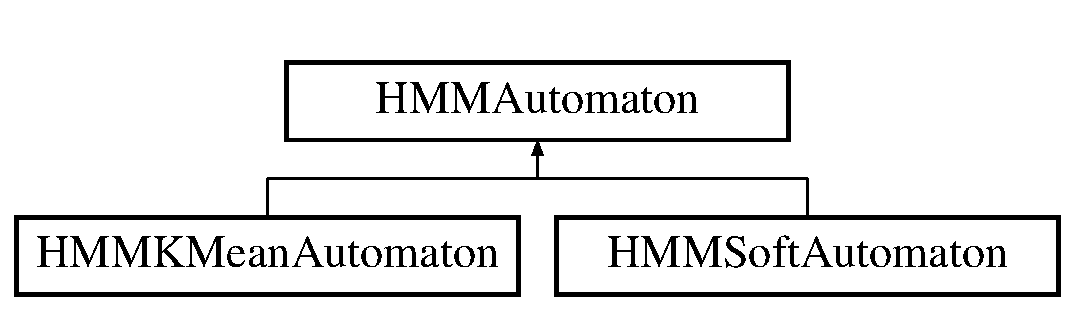
\includegraphics[height=2.000000cm]{class_h_m_m_automaton}
\end{center}
\end{figure}
\subsection*{Public Types}
\begin{DoxyCompactItemize}
\item 
enum \hyperlink{class_h_m_m_automaton_aa3476c86db5e0791de6f07076f220348}{T\+R\+A\+I\+N\+\_\+\+T\+Y\+P\+E} \{ \hyperlink{class_h_m_m_automaton_aa3476c86db5e0791de6f07076f220348a725fd42edf8b8e4b515b6296a7d67bb3}{S\+E\+G}, 
\hyperlink{class_h_m_m_automaton_aa3476c86db5e0791de6f07076f220348a0dde40730a38683ab3845601ec57591b}{S\+E\+Q}
 \}
\end{DoxyCompactItemize}
\subsection*{Public Member Functions}
\begin{DoxyCompactItemize}
\item 
\hyperlink{class_h_m_m_automaton_a27cacf1d1e73c9b48cf614f1c8b8921c}{H\+M\+M\+Automaton} (std\+::vector$<$ \hyperlink{class_wave_feature_o_p}{Wave\+Feature\+O\+P} $>$ $\ast$feature, int state\+Num=\hyperlink{configure__hmm_8h_aa9cc71cb42394379957677c761aae79e}{A\+U\+T\+O\+M\+A\+T\+O\+N\+\_\+\+S\+T\+A\+T\+E\+\_\+\+N\+U\+M}, int \hyperlink{pro6__demo_8cpp_a923ffcfa3c56ccdba17bc4e700247d54}{gauss\+Num}=\hyperlink{configure__hmm_8h_a8f9db0624fff0b17f641785bb8d66a82}{G\+A\+U\+S\+S\+I\+A\+N\+\_\+\+N\+U\+M}, int train\+Times=\hyperlink{configure__hmm_8h_a52e22519b5a37e58632e9183d5197b86}{M\+A\+X\+\_\+\+T\+R\+A\+I\+N\+\_\+\+T\+I\+M\+E\+S})
\item 
virtual \hyperlink{class_h_m_m_automaton_aceb16780fdcef5093d0e9faca938757d}{$\sim$\+H\+M\+M\+Automaton} ()
\item 
virtual void \hyperlink{class_h_m_m_automaton_ac6bbc2770cb11b1c9e55cd0652fbe0e3}{hmm\+Train} ()=0
\item 
virtual double \hyperlink{class_h_m_m_automaton_a4c43e2b6bba8c6f237bf4503d79b1f12}{calc\+Cost} (\hyperlink{class_wave_feature_o_p}{Wave\+Feature\+O\+P} \&input)=0
\item 
void \hyperlink{class_h_m_m_automaton_ac4deb72548be0ec35f83adc374518986}{close} ()
\item 
void \hyperlink{class_h_m_m_automaton_a522f7a4ffa67d79d9303be3e602c7f88}{adjust\+Skipping\+Transfer} ()
\item 
virtual void \hyperlink{class_h_m_m_automaton_a04b64e19e77d5fe8b78d471470346872}{load} (std\+::stringstream \&in)=0
\item 
void \hyperlink{class_h_m_m_automaton_a55a1374058fe22b69eceea075cf4c68f}{store} (std\+::stringstream \&out)
\item 
void \hyperlink{class_h_m_m_automaton_a46af46bd5a90c22ecea1076805e595d0}{dump\+Transfer} (std\+::ostream \&out)
\item 
double \hyperlink{class_h_m_m_automaton_a8e3043723eb18068bb5cb9840f844647}{endding\+Probability} (int state\+I\+D)
\item 
void \hyperlink{class_h_m_m_automaton_a6aa2c2115023896733005f050097a457}{set\+Templates} (std\+::vector$<$ \hyperlink{class_wave_feature_o_p}{Wave\+Feature\+O\+P} $>$ $\ast$new\+Temps)
\end{DoxyCompactItemize}
\subsection*{Protected Types}
\begin{DoxyCompactItemize}
\item 
enum \hyperlink{class_h_m_m_automaton_a971e23dcda492fc9f32b1cddf6822fd2}{dtw\+Type} \{ \hyperlink{class_h_m_m_automaton_a971e23dcda492fc9f32b1cddf6822fd2a2427c9ba053ced14af44df842e351bfa}{Maximum}, 
\hyperlink{class_h_m_m_automaton_a971e23dcda492fc9f32b1cddf6822fd2a749fd94f15dc2e53ed8b3dcdbddd6d88}{Sigma}
 \}
\end{DoxyCompactItemize}
\subsection*{Protected Member Functions}
\begin{DoxyCompactItemize}
\item 
bool \hyperlink{class_h_m_m_automaton_a836856d9c7539cc2b25bc72dc8f96b7d}{is\+Big\+Change} (double total\+Change\+Cost)
\item 
void \hyperlink{class_h_m_m_automaton_a15856e4c7e4a7322d5a2bf15e9cd7440}{roll\+Dtw\+Init} (\hyperlink{class_wave_feature_o_p}{Wave\+Feature\+O\+P} \&\hyperlink{lpc2cep_8m_afcc1d2df0288347ea10603033506e33b}{features}, \hyperlink{class_h_m_m_automaton_a971e23dcda492fc9f32b1cddf6822fd2}{dtw\+Type} \hyperlink{readhtk_8m_ac7798f4aec24aa6076b2b222bd91d4fd}{type})
\item 
std\+::pair$<$ int, double $>$ \hyperlink{class_h_m_m_automaton_a6fb93aa0899b5725eb435708e704df0f}{roll\+Dtw} (\hyperlink{class_wave_feature_o_p}{Wave\+Feature\+O\+P} \&\hyperlink{lpc2cep_8m_afcc1d2df0288347ea10603033506e33b}{features}, \hyperlink{class_h_m_m_automaton_a971e23dcda492fc9f32b1cddf6822fd2}{dtw\+Type} \hyperlink{readhtk_8m_ac7798f4aec24aa6076b2b222bd91d4fd}{type})
\item 
void \hyperlink{class_h_m_m_automaton_a06f4a989be46476c329be70ac78de820}{clear\+States} ()
\item 
int \hyperlink{class_h_m_m_automaton_a500df5c237ddb079ffe4e36a0a55fbcd}{get\+Roll\+Idx} (int column\+Idx)
\item 
void \hyperlink{class_h_m_m_automaton_a48b81c61396a1d2e84827c5a35c9927b}{Init} ()
\end{DoxyCompactItemize}
\subsection*{Protected Attributes}
\begin{DoxyCompactItemize}
\item 
\hyperlink{configure__basic_8h_a566a006016cf65b1b01bd2bc633e1c12}{Matrix}$<$ int $>$ \hyperlink{class_h_m_m_automaton_a231123e55258281030977666a4f20eb2}{path}
\item 
std\+::vector$<$ double $>$ \hyperlink{class_h_m_m_automaton_a17bbaefff43e3a67f6c3614b6ccdac9c}{roll\+Column\+Cost} \mbox{[}2\mbox{]}
\item 
std\+::vector$<$ \hyperlink{class_wave_feature_o_p}{Wave\+Feature\+O\+P} $>$ $\ast$ \hyperlink{class_h_m_m_automaton_a9932eb5aa8ff484ac2406f98498595cf}{templates}
\item 
\hyperlink{configure__basic_8h_a566a006016cf65b1b01bd2bc633e1c12}{Matrix}$<$ double $>$ \hyperlink{class_h_m_m_automaton_af2b7d9675b77191e808e8a0501313f69}{transfer\+Cost}
\item 
std\+::vector$<$ \hyperlink{class_h_m_m_state}{H\+M\+M\+State} $\ast$ $>$ \hyperlink{class_h_m_m_automaton_a3ffe1d6d2d66c2bcfefb1339140c513b}{states}
\end{DoxyCompactItemize}
\subsection*{Private Member Functions}
\begin{DoxyCompactItemize}
\item 
\hyperlink{class_h_m_m_automaton_a7338d8ef8f07f6e625b088e79f3da96d}{R\+E\+A\+D\+\_\+\+W\+R\+I\+T\+E\+\_\+\+D\+E\+C\+L\+A\+R\+E} (int, state\+Num, State\+Num)
\item 
\hyperlink{class_h_m_m_automaton_aeb3e5fa260e4a3e321ef793013a270d6}{R\+E\+A\+D\+\_\+\+W\+R\+I\+T\+E\+\_\+\+D\+E\+C\+L\+A\+R\+E} (int, \hyperlink{pro6__demo_8cpp_a923ffcfa3c56ccdba17bc4e700247d54}{gauss\+Num}, Gauss\+Num)
\item 
\hyperlink{class_h_m_m_automaton_ae7f461bacc7daf2d3c2f4b7f233e0cef}{R\+E\+A\+D\+\_\+\+W\+R\+I\+T\+E\+\_\+\+D\+E\+C\+L\+A\+R\+E} (int, train\+Times, Train\+Times)
\end{DoxyCompactItemize}
\subsection*{Friends}
\begin{DoxyCompactItemize}
\item 
class \hyperlink{class_h_m_m_automaton_a1b622e128d992231899ba78ca9c72507}{Seq\+Model}
\end{DoxyCompactItemize}


\subsection{Member Enumeration Documentation}
\hypertarget{class_h_m_m_automaton_a971e23dcda492fc9f32b1cddf6822fd2}{\index{H\+M\+M\+Automaton@{H\+M\+M\+Automaton}!dtw\+Type@{dtw\+Type}}
\index{dtw\+Type@{dtw\+Type}!H\+M\+M\+Automaton@{H\+M\+M\+Automaton}}
\subsubsection[{dtw\+Type}]{\setlength{\rightskip}{0pt plus 5cm}enum {\bf H\+M\+M\+Automaton\+::dtw\+Type}\hspace{0.3cm}{\ttfamily [protected]}}}\label{class_h_m_m_automaton_a971e23dcda492fc9f32b1cddf6822fd2}
\begin{Desc}
\item[Enumerator]\par
\begin{description}
\index{Maximum@{Maximum}!H\+M\+M\+Automaton@{H\+M\+M\+Automaton}}\index{H\+M\+M\+Automaton@{H\+M\+M\+Automaton}!Maximum@{Maximum}}\item[{\em 
\hypertarget{class_h_m_m_automaton_a971e23dcda492fc9f32b1cddf6822fd2a2427c9ba053ced14af44df842e351bfa}{Maximum}\label{class_h_m_m_automaton_a971e23dcda492fc9f32b1cddf6822fd2a2427c9ba053ced14af44df842e351bfa}
}]\index{Sigma@{Sigma}!H\+M\+M\+Automaton@{H\+M\+M\+Automaton}}\index{H\+M\+M\+Automaton@{H\+M\+M\+Automaton}!Sigma@{Sigma}}\item[{\em 
\hypertarget{class_h_m_m_automaton_a971e23dcda492fc9f32b1cddf6822fd2a749fd94f15dc2e53ed8b3dcdbddd6d88}{Sigma}\label{class_h_m_m_automaton_a971e23dcda492fc9f32b1cddf6822fd2a749fd94f15dc2e53ed8b3dcdbddd6d88}
}]\end{description}
\end{Desc}
\hypertarget{class_h_m_m_automaton_aa3476c86db5e0791de6f07076f220348}{\index{H\+M\+M\+Automaton@{H\+M\+M\+Automaton}!T\+R\+A\+I\+N\+\_\+\+T\+Y\+P\+E@{T\+R\+A\+I\+N\+\_\+\+T\+Y\+P\+E}}
\index{T\+R\+A\+I\+N\+\_\+\+T\+Y\+P\+E@{T\+R\+A\+I\+N\+\_\+\+T\+Y\+P\+E}!H\+M\+M\+Automaton@{H\+M\+M\+Automaton}}
\subsubsection[{T\+R\+A\+I\+N\+\_\+\+T\+Y\+P\+E}]{\setlength{\rightskip}{0pt plus 5cm}enum {\bf H\+M\+M\+Automaton\+::\+T\+R\+A\+I\+N\+\_\+\+T\+Y\+P\+E}}}\label{class_h_m_m_automaton_aa3476c86db5e0791de6f07076f220348}
\begin{Desc}
\item[Enumerator]\par
\begin{description}
\index{S\+E\+G@{S\+E\+G}!H\+M\+M\+Automaton@{H\+M\+M\+Automaton}}\index{H\+M\+M\+Automaton@{H\+M\+M\+Automaton}!S\+E\+G@{S\+E\+G}}\item[{\em 
\hypertarget{class_h_m_m_automaton_aa3476c86db5e0791de6f07076f220348a725fd42edf8b8e4b515b6296a7d67bb3}{S\+E\+G}\label{class_h_m_m_automaton_aa3476c86db5e0791de6f07076f220348a725fd42edf8b8e4b515b6296a7d67bb3}
}]\index{S\+E\+Q@{S\+E\+Q}!H\+M\+M\+Automaton@{H\+M\+M\+Automaton}}\index{H\+M\+M\+Automaton@{H\+M\+M\+Automaton}!S\+E\+Q@{S\+E\+Q}}\item[{\em 
\hypertarget{class_h_m_m_automaton_aa3476c86db5e0791de6f07076f220348a0dde40730a38683ab3845601ec57591b}{S\+E\+Q}\label{class_h_m_m_automaton_aa3476c86db5e0791de6f07076f220348a0dde40730a38683ab3845601ec57591b}
}]\end{description}
\end{Desc}


\subsection{Constructor \& Destructor Documentation}
\hypertarget{class_h_m_m_automaton_a27cacf1d1e73c9b48cf614f1c8b8921c}{\index{H\+M\+M\+Automaton@{H\+M\+M\+Automaton}!H\+M\+M\+Automaton@{H\+M\+M\+Automaton}}
\index{H\+M\+M\+Automaton@{H\+M\+M\+Automaton}!H\+M\+M\+Automaton@{H\+M\+M\+Automaton}}
\subsubsection[{H\+M\+M\+Automaton}]{\setlength{\rightskip}{0pt plus 5cm}H\+M\+M\+Automaton\+::\+H\+M\+M\+Automaton (
\begin{DoxyParamCaption}
\item[{std\+::vector$<$ {\bf Wave\+Feature\+O\+P} $>$ $\ast$}]{feature, }
\item[{int}]{state\+Num = {\ttfamily {\bf A\+U\+T\+O\+M\+A\+T\+O\+N\+\_\+\+S\+T\+A\+T\+E\+\_\+\+N\+U\+M}}, }
\item[{int}]{gauss\+Num = {\ttfamily {\bf G\+A\+U\+S\+S\+I\+A\+N\+\_\+\+N\+U\+M}}, }
\item[{int}]{train\+Times = {\ttfamily {\bf M\+A\+X\+\_\+\+T\+R\+A\+I\+N\+\_\+\+T\+I\+M\+E\+S}}}
\end{DoxyParamCaption}
)}}\label{class_h_m_m_automaton_a27cacf1d1e73c9b48cf614f1c8b8921c}
\hypertarget{class_h_m_m_automaton_aceb16780fdcef5093d0e9faca938757d}{\index{H\+M\+M\+Automaton@{H\+M\+M\+Automaton}!````~H\+M\+M\+Automaton@{$\sim$\+H\+M\+M\+Automaton}}
\index{````~H\+M\+M\+Automaton@{$\sim$\+H\+M\+M\+Automaton}!H\+M\+M\+Automaton@{H\+M\+M\+Automaton}}
\subsubsection[{$\sim$\+H\+M\+M\+Automaton}]{\setlength{\rightskip}{0pt plus 5cm}virtual H\+M\+M\+Automaton\+::$\sim$\+H\+M\+M\+Automaton (
\begin{DoxyParamCaption}
{}
\end{DoxyParamCaption}
)\hspace{0.3cm}{\ttfamily [inline]}, {\ttfamily [virtual]}}}\label{class_h_m_m_automaton_aceb16780fdcef5093d0e9faca938757d}


\subsection{Member Function Documentation}
\hypertarget{class_h_m_m_automaton_a522f7a4ffa67d79d9303be3e602c7f88}{\index{H\+M\+M\+Automaton@{H\+M\+M\+Automaton}!adjust\+Skipping\+Transfer@{adjust\+Skipping\+Transfer}}
\index{adjust\+Skipping\+Transfer@{adjust\+Skipping\+Transfer}!H\+M\+M\+Automaton@{H\+M\+M\+Automaton}}
\subsubsection[{adjust\+Skipping\+Transfer}]{\setlength{\rightskip}{0pt plus 5cm}void H\+M\+M\+Automaton\+::adjust\+Skipping\+Transfer (
\begin{DoxyParamCaption}
{}
\end{DoxyParamCaption}
)}}\label{class_h_m_m_automaton_a522f7a4ffa67d79d9303be3e602c7f88}
\hypertarget{class_h_m_m_automaton_a4c43e2b6bba8c6f237bf4503d79b1f12}{\index{H\+M\+M\+Automaton@{H\+M\+M\+Automaton}!calc\+Cost@{calc\+Cost}}
\index{calc\+Cost@{calc\+Cost}!H\+M\+M\+Automaton@{H\+M\+M\+Automaton}}
\subsubsection[{calc\+Cost}]{\setlength{\rightskip}{0pt plus 5cm}virtual double H\+M\+M\+Automaton\+::calc\+Cost (
\begin{DoxyParamCaption}
\item[{{\bf Wave\+Feature\+O\+P} \&}]{input}
\end{DoxyParamCaption}
)\hspace{0.3cm}{\ttfamily [pure virtual]}}}\label{class_h_m_m_automaton_a4c43e2b6bba8c6f237bf4503d79b1f12}


Implemented in \hyperlink{class_h_m_m_soft_automaton_a4efa065f2e067d9e0b71bbf4a25bd120}{H\+M\+M\+Soft\+Automaton}, and \hyperlink{class_h_m_m_k_mean_automaton_a65df5f2b00684dc7dbfd14f5980ce5b9}{H\+M\+M\+K\+Mean\+Automaton}.

\hypertarget{class_h_m_m_automaton_a06f4a989be46476c329be70ac78de820}{\index{H\+M\+M\+Automaton@{H\+M\+M\+Automaton}!clear\+States@{clear\+States}}
\index{clear\+States@{clear\+States}!H\+M\+M\+Automaton@{H\+M\+M\+Automaton}}
\subsubsection[{clear\+States}]{\setlength{\rightskip}{0pt plus 5cm}void H\+M\+M\+Automaton\+::clear\+States (
\begin{DoxyParamCaption}
{}
\end{DoxyParamCaption}
)\hspace{0.3cm}{\ttfamily [protected]}}}\label{class_h_m_m_automaton_a06f4a989be46476c329be70ac78de820}
\hypertarget{class_h_m_m_automaton_ac4deb72548be0ec35f83adc374518986}{\index{H\+M\+M\+Automaton@{H\+M\+M\+Automaton}!close@{close}}
\index{close@{close}!H\+M\+M\+Automaton@{H\+M\+M\+Automaton}}
\subsubsection[{close}]{\setlength{\rightskip}{0pt plus 5cm}void H\+M\+M\+Automaton\+::close (
\begin{DoxyParamCaption}
{}
\end{DoxyParamCaption}
)}}\label{class_h_m_m_automaton_ac4deb72548be0ec35f83adc374518986}
\hypertarget{class_h_m_m_automaton_a46af46bd5a90c22ecea1076805e595d0}{\index{H\+M\+M\+Automaton@{H\+M\+M\+Automaton}!dump\+Transfer@{dump\+Transfer}}
\index{dump\+Transfer@{dump\+Transfer}!H\+M\+M\+Automaton@{H\+M\+M\+Automaton}}
\subsubsection[{dump\+Transfer}]{\setlength{\rightskip}{0pt plus 5cm}void H\+M\+M\+Automaton\+::dump\+Transfer (
\begin{DoxyParamCaption}
\item[{std\+::ostream \&}]{out}
\end{DoxyParamCaption}
)}}\label{class_h_m_m_automaton_a46af46bd5a90c22ecea1076805e595d0}
\hypertarget{class_h_m_m_automaton_a8e3043723eb18068bb5cb9840f844647}{\index{H\+M\+M\+Automaton@{H\+M\+M\+Automaton}!endding\+Probability@{endding\+Probability}}
\index{endding\+Probability@{endding\+Probability}!H\+M\+M\+Automaton@{H\+M\+M\+Automaton}}
\subsubsection[{endding\+Probability}]{\setlength{\rightskip}{0pt plus 5cm}double H\+M\+M\+Automaton\+::endding\+Probability (
\begin{DoxyParamCaption}
\item[{int}]{state\+I\+D}
\end{DoxyParamCaption}
)}}\label{class_h_m_m_automaton_a8e3043723eb18068bb5cb9840f844647}
\hypertarget{class_h_m_m_automaton_a500df5c237ddb079ffe4e36a0a55fbcd}{\index{H\+M\+M\+Automaton@{H\+M\+M\+Automaton}!get\+Roll\+Idx@{get\+Roll\+Idx}}
\index{get\+Roll\+Idx@{get\+Roll\+Idx}!H\+M\+M\+Automaton@{H\+M\+M\+Automaton}}
\subsubsection[{get\+Roll\+Idx}]{\setlength{\rightskip}{0pt plus 5cm}int H\+M\+M\+Automaton\+::get\+Roll\+Idx (
\begin{DoxyParamCaption}
\item[{int}]{column\+Idx}
\end{DoxyParamCaption}
)\hspace{0.3cm}{\ttfamily [inline]}, {\ttfamily [protected]}}}\label{class_h_m_m_automaton_a500df5c237ddb079ffe4e36a0a55fbcd}
\hypertarget{class_h_m_m_automaton_ac6bbc2770cb11b1c9e55cd0652fbe0e3}{\index{H\+M\+M\+Automaton@{H\+M\+M\+Automaton}!hmm\+Train@{hmm\+Train}}
\index{hmm\+Train@{hmm\+Train}!H\+M\+M\+Automaton@{H\+M\+M\+Automaton}}
\subsubsection[{hmm\+Train}]{\setlength{\rightskip}{0pt plus 5cm}virtual void H\+M\+M\+Automaton\+::hmm\+Train (
\begin{DoxyParamCaption}
{}
\end{DoxyParamCaption}
)\hspace{0.3cm}{\ttfamily [pure virtual]}}}\label{class_h_m_m_automaton_ac6bbc2770cb11b1c9e55cd0652fbe0e3}


Implemented in \hyperlink{class_h_m_m_soft_automaton_a06c50e4f7a3461a6c6737cbe077ca0d0}{H\+M\+M\+Soft\+Automaton}, and \hyperlink{class_h_m_m_k_mean_automaton_a1123c813c91a51bf9d2b9ad9043bbdf8}{H\+M\+M\+K\+Mean\+Automaton}.

\hypertarget{class_h_m_m_automaton_a48b81c61396a1d2e84827c5a35c9927b}{\index{H\+M\+M\+Automaton@{H\+M\+M\+Automaton}!Init@{Init}}
\index{Init@{Init}!H\+M\+M\+Automaton@{H\+M\+M\+Automaton}}
\subsubsection[{Init}]{\setlength{\rightskip}{0pt plus 5cm}void H\+M\+M\+Automaton\+::\+Init (
\begin{DoxyParamCaption}
{}
\end{DoxyParamCaption}
)\hspace{0.3cm}{\ttfamily [inline]}, {\ttfamily [protected]}}}\label{class_h_m_m_automaton_a48b81c61396a1d2e84827c5a35c9927b}
\hypertarget{class_h_m_m_automaton_a836856d9c7539cc2b25bc72dc8f96b7d}{\index{H\+M\+M\+Automaton@{H\+M\+M\+Automaton}!is\+Big\+Change@{is\+Big\+Change}}
\index{is\+Big\+Change@{is\+Big\+Change}!H\+M\+M\+Automaton@{H\+M\+M\+Automaton}}
\subsubsection[{is\+Big\+Change}]{\setlength{\rightskip}{0pt plus 5cm}bool H\+M\+M\+Automaton\+::is\+Big\+Change (
\begin{DoxyParamCaption}
\item[{double}]{total\+Change\+Cost}
\end{DoxyParamCaption}
)\hspace{0.3cm}{\ttfamily [inline]}, {\ttfamily [protected]}}}\label{class_h_m_m_automaton_a836856d9c7539cc2b25bc72dc8f96b7d}
\hypertarget{class_h_m_m_automaton_a04b64e19e77d5fe8b78d471470346872}{\index{H\+M\+M\+Automaton@{H\+M\+M\+Automaton}!load@{load}}
\index{load@{load}!H\+M\+M\+Automaton@{H\+M\+M\+Automaton}}
\subsubsection[{load}]{\setlength{\rightskip}{0pt plus 5cm}virtual void H\+M\+M\+Automaton\+::load (
\begin{DoxyParamCaption}
\item[{std\+::stringstream \&}]{in}
\end{DoxyParamCaption}
)\hspace{0.3cm}{\ttfamily [pure virtual]}}}\label{class_h_m_m_automaton_a04b64e19e77d5fe8b78d471470346872}


Implemented in \hyperlink{class_h_m_m_k_mean_automaton_a967fcfe7e5e00fd427df2d3f2ce313dc}{H\+M\+M\+K\+Mean\+Automaton}, and \hyperlink{class_h_m_m_soft_automaton_ac99d24cfbfa563c54a6ee7c68b36d37e}{H\+M\+M\+Soft\+Automaton}.

\hypertarget{class_h_m_m_automaton_a7338d8ef8f07f6e625b088e79f3da96d}{\index{H\+M\+M\+Automaton@{H\+M\+M\+Automaton}!R\+E\+A\+D\+\_\+\+W\+R\+I\+T\+E\+\_\+\+D\+E\+C\+L\+A\+R\+E@{R\+E\+A\+D\+\_\+\+W\+R\+I\+T\+E\+\_\+\+D\+E\+C\+L\+A\+R\+E}}
\index{R\+E\+A\+D\+\_\+\+W\+R\+I\+T\+E\+\_\+\+D\+E\+C\+L\+A\+R\+E@{R\+E\+A\+D\+\_\+\+W\+R\+I\+T\+E\+\_\+\+D\+E\+C\+L\+A\+R\+E}!H\+M\+M\+Automaton@{H\+M\+M\+Automaton}}
\subsubsection[{R\+E\+A\+D\+\_\+\+W\+R\+I\+T\+E\+\_\+\+D\+E\+C\+L\+A\+R\+E}]{\setlength{\rightskip}{0pt plus 5cm}H\+M\+M\+Automaton\+::\+R\+E\+A\+D\+\_\+\+W\+R\+I\+T\+E\+\_\+\+D\+E\+C\+L\+A\+R\+E (
\begin{DoxyParamCaption}
\item[{int}]{, }
\item[{state\+Num}]{, }
\item[{State\+Num}]{}
\end{DoxyParamCaption}
)\hspace{0.3cm}{\ttfamily [private]}}}\label{class_h_m_m_automaton_a7338d8ef8f07f6e625b088e79f3da96d}
\hypertarget{class_h_m_m_automaton_aeb3e5fa260e4a3e321ef793013a270d6}{\index{H\+M\+M\+Automaton@{H\+M\+M\+Automaton}!R\+E\+A\+D\+\_\+\+W\+R\+I\+T\+E\+\_\+\+D\+E\+C\+L\+A\+R\+E@{R\+E\+A\+D\+\_\+\+W\+R\+I\+T\+E\+\_\+\+D\+E\+C\+L\+A\+R\+E}}
\index{R\+E\+A\+D\+\_\+\+W\+R\+I\+T\+E\+\_\+\+D\+E\+C\+L\+A\+R\+E@{R\+E\+A\+D\+\_\+\+W\+R\+I\+T\+E\+\_\+\+D\+E\+C\+L\+A\+R\+E}!H\+M\+M\+Automaton@{H\+M\+M\+Automaton}}
\subsubsection[{R\+E\+A\+D\+\_\+\+W\+R\+I\+T\+E\+\_\+\+D\+E\+C\+L\+A\+R\+E}]{\setlength{\rightskip}{0pt plus 5cm}H\+M\+M\+Automaton\+::\+R\+E\+A\+D\+\_\+\+W\+R\+I\+T\+E\+\_\+\+D\+E\+C\+L\+A\+R\+E (
\begin{DoxyParamCaption}
\item[{int}]{, }
\item[{{\bf gauss\+Num}}]{, }
\item[{Gauss\+Num}]{}
\end{DoxyParamCaption}
)\hspace{0.3cm}{\ttfamily [private]}}}\label{class_h_m_m_automaton_aeb3e5fa260e4a3e321ef793013a270d6}
\hypertarget{class_h_m_m_automaton_ae7f461bacc7daf2d3c2f4b7f233e0cef}{\index{H\+M\+M\+Automaton@{H\+M\+M\+Automaton}!R\+E\+A\+D\+\_\+\+W\+R\+I\+T\+E\+\_\+\+D\+E\+C\+L\+A\+R\+E@{R\+E\+A\+D\+\_\+\+W\+R\+I\+T\+E\+\_\+\+D\+E\+C\+L\+A\+R\+E}}
\index{R\+E\+A\+D\+\_\+\+W\+R\+I\+T\+E\+\_\+\+D\+E\+C\+L\+A\+R\+E@{R\+E\+A\+D\+\_\+\+W\+R\+I\+T\+E\+\_\+\+D\+E\+C\+L\+A\+R\+E}!H\+M\+M\+Automaton@{H\+M\+M\+Automaton}}
\subsubsection[{R\+E\+A\+D\+\_\+\+W\+R\+I\+T\+E\+\_\+\+D\+E\+C\+L\+A\+R\+E}]{\setlength{\rightskip}{0pt plus 5cm}H\+M\+M\+Automaton\+::\+R\+E\+A\+D\+\_\+\+W\+R\+I\+T\+E\+\_\+\+D\+E\+C\+L\+A\+R\+E (
\begin{DoxyParamCaption}
\item[{int}]{, }
\item[{train\+Times}]{, }
\item[{Train\+Times}]{}
\end{DoxyParamCaption}
)\hspace{0.3cm}{\ttfamily [private]}}}\label{class_h_m_m_automaton_ae7f461bacc7daf2d3c2f4b7f233e0cef}
\hypertarget{class_h_m_m_automaton_a6fb93aa0899b5725eb435708e704df0f}{\index{H\+M\+M\+Automaton@{H\+M\+M\+Automaton}!roll\+Dtw@{roll\+Dtw}}
\index{roll\+Dtw@{roll\+Dtw}!H\+M\+M\+Automaton@{H\+M\+M\+Automaton}}
\subsubsection[{roll\+Dtw}]{\setlength{\rightskip}{0pt plus 5cm}std\+::pair$<$int, double$>$ H\+M\+M\+Automaton\+::roll\+Dtw (
\begin{DoxyParamCaption}
\item[{{\bf Wave\+Feature\+O\+P} \&}]{features, }
\item[{{\bf dtw\+Type}}]{type}
\end{DoxyParamCaption}
)\hspace{0.3cm}{\ttfamily [inline]}, {\ttfamily [protected]}}}\label{class_h_m_m_automaton_a6fb93aa0899b5725eb435708e704df0f}
\hypertarget{class_h_m_m_automaton_a15856e4c7e4a7322d5a2bf15e9cd7440}{\index{H\+M\+M\+Automaton@{H\+M\+M\+Automaton}!roll\+Dtw\+Init@{roll\+Dtw\+Init}}
\index{roll\+Dtw\+Init@{roll\+Dtw\+Init}!H\+M\+M\+Automaton@{H\+M\+M\+Automaton}}
\subsubsection[{roll\+Dtw\+Init}]{\setlength{\rightskip}{0pt plus 5cm}void H\+M\+M\+Automaton\+::roll\+Dtw\+Init (
\begin{DoxyParamCaption}
\item[{{\bf Wave\+Feature\+O\+P} \&}]{features, }
\item[{{\bf dtw\+Type}}]{type}
\end{DoxyParamCaption}
)\hspace{0.3cm}{\ttfamily [inline]}, {\ttfamily [protected]}}}\label{class_h_m_m_automaton_a15856e4c7e4a7322d5a2bf15e9cd7440}
\hypertarget{class_h_m_m_automaton_a6aa2c2115023896733005f050097a457}{\index{H\+M\+M\+Automaton@{H\+M\+M\+Automaton}!set\+Templates@{set\+Templates}}
\index{set\+Templates@{set\+Templates}!H\+M\+M\+Automaton@{H\+M\+M\+Automaton}}
\subsubsection[{set\+Templates}]{\setlength{\rightskip}{0pt plus 5cm}void H\+M\+M\+Automaton\+::set\+Templates (
\begin{DoxyParamCaption}
\item[{std\+::vector$<$ {\bf Wave\+Feature\+O\+P} $>$ $\ast$}]{new\+Temps}
\end{DoxyParamCaption}
)\hspace{0.3cm}{\ttfamily [inline]}}}\label{class_h_m_m_automaton_a6aa2c2115023896733005f050097a457}
\hypertarget{class_h_m_m_automaton_a55a1374058fe22b69eceea075cf4c68f}{\index{H\+M\+M\+Automaton@{H\+M\+M\+Automaton}!store@{store}}
\index{store@{store}!H\+M\+M\+Automaton@{H\+M\+M\+Automaton}}
\subsubsection[{store}]{\setlength{\rightskip}{0pt plus 5cm}void H\+M\+M\+Automaton\+::store (
\begin{DoxyParamCaption}
\item[{std\+::stringstream \&}]{out}
\end{DoxyParamCaption}
)}}\label{class_h_m_m_automaton_a55a1374058fe22b69eceea075cf4c68f}


\subsection{Friends And Related Function Documentation}
\hypertarget{class_h_m_m_automaton_a1b622e128d992231899ba78ca9c72507}{\index{H\+M\+M\+Automaton@{H\+M\+M\+Automaton}!Seq\+Model@{Seq\+Model}}
\index{Seq\+Model@{Seq\+Model}!H\+M\+M\+Automaton@{H\+M\+M\+Automaton}}
\subsubsection[{Seq\+Model}]{\setlength{\rightskip}{0pt plus 5cm}friend class {\bf Seq\+Model}\hspace{0.3cm}{\ttfamily [friend]}}}\label{class_h_m_m_automaton_a1b622e128d992231899ba78ca9c72507}


\subsection{Member Data Documentation}
\hypertarget{class_h_m_m_automaton_a231123e55258281030977666a4f20eb2}{\index{H\+M\+M\+Automaton@{H\+M\+M\+Automaton}!path@{path}}
\index{path@{path}!H\+M\+M\+Automaton@{H\+M\+M\+Automaton}}
\subsubsection[{path}]{\setlength{\rightskip}{0pt plus 5cm}{\bf Matrix}$<$int$>$ H\+M\+M\+Automaton\+::path\hspace{0.3cm}{\ttfamily [protected]}}}\label{class_h_m_m_automaton_a231123e55258281030977666a4f20eb2}
\hypertarget{class_h_m_m_automaton_a17bbaefff43e3a67f6c3614b6ccdac9c}{\index{H\+M\+M\+Automaton@{H\+M\+M\+Automaton}!roll\+Column\+Cost@{roll\+Column\+Cost}}
\index{roll\+Column\+Cost@{roll\+Column\+Cost}!H\+M\+M\+Automaton@{H\+M\+M\+Automaton}}
\subsubsection[{roll\+Column\+Cost}]{\setlength{\rightskip}{0pt plus 5cm}std\+::vector$<$double$>$ H\+M\+M\+Automaton\+::roll\+Column\+Cost\mbox{[}2\mbox{]}\hspace{0.3cm}{\ttfamily [protected]}}}\label{class_h_m_m_automaton_a17bbaefff43e3a67f6c3614b6ccdac9c}
\hypertarget{class_h_m_m_automaton_a3ffe1d6d2d66c2bcfefb1339140c513b}{\index{H\+M\+M\+Automaton@{H\+M\+M\+Automaton}!states@{states}}
\index{states@{states}!H\+M\+M\+Automaton@{H\+M\+M\+Automaton}}
\subsubsection[{states}]{\setlength{\rightskip}{0pt plus 5cm}std\+::vector$<${\bf H\+M\+M\+State} $\ast$$>$ H\+M\+M\+Automaton\+::states\hspace{0.3cm}{\ttfamily [protected]}}}\label{class_h_m_m_automaton_a3ffe1d6d2d66c2bcfefb1339140c513b}
\hypertarget{class_h_m_m_automaton_a9932eb5aa8ff484ac2406f98498595cf}{\index{H\+M\+M\+Automaton@{H\+M\+M\+Automaton}!templates@{templates}}
\index{templates@{templates}!H\+M\+M\+Automaton@{H\+M\+M\+Automaton}}
\subsubsection[{templates}]{\setlength{\rightskip}{0pt plus 5cm}std\+::vector$<${\bf Wave\+Feature\+O\+P}$>$$\ast$ H\+M\+M\+Automaton\+::templates\hspace{0.3cm}{\ttfamily [protected]}}}\label{class_h_m_m_automaton_a9932eb5aa8ff484ac2406f98498595cf}
\hypertarget{class_h_m_m_automaton_af2b7d9675b77191e808e8a0501313f69}{\index{H\+M\+M\+Automaton@{H\+M\+M\+Automaton}!transfer\+Cost@{transfer\+Cost}}
\index{transfer\+Cost@{transfer\+Cost}!H\+M\+M\+Automaton@{H\+M\+M\+Automaton}}
\subsubsection[{transfer\+Cost}]{\setlength{\rightskip}{0pt plus 5cm}{\bf Matrix}$<$double$>$ H\+M\+M\+Automaton\+::transfer\+Cost\hspace{0.3cm}{\ttfamily [protected]}}}\label{class_h_m_m_automaton_af2b7d9675b77191e808e8a0501313f69}


The documentation for this class was generated from the following files\+:\begin{DoxyCompactItemize}
\item 
src/\+Feature/\hyperlink{_h_m_m_automaton_8h}{H\+M\+M\+Automaton.\+h}\item 
src/\+Feature/\hyperlink{_h_m_m_automaton_8cpp}{H\+M\+M\+Automaton.\+cpp}\end{DoxyCompactItemize}

\hypertarget{class_h_m_m_automaton_set}{\section{H\+M\+M\+Automaton\+Set Class Reference}
\label{class_h_m_m_automaton_set}\index{H\+M\+M\+Automaton\+Set@{H\+M\+M\+Automaton\+Set}}
}


{\ttfamily \#include $<$H\+M\+M\+Automaton\+Set.\+h$>$}

Inheritance diagram for H\+M\+M\+Automaton\+Set\+:\begin{figure}[H]
\begin{center}
\leavevmode
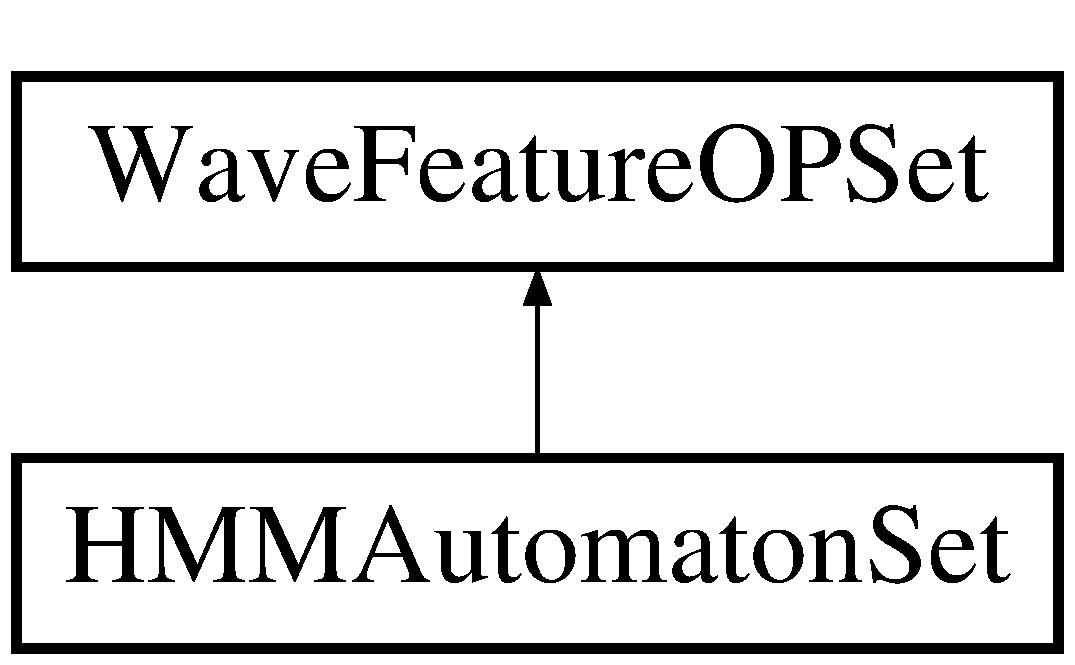
\includegraphics[height=2.000000cm]{class_h_m_m_automaton_set}
\end{center}
\end{figure}
\subsection*{Public Member Functions}
\begin{DoxyCompactItemize}
\item 
\hyperlink{class_h_m_m_automaton_set_afa2bb2913d8c0db8342ddd8bd7e1bb04}{H\+M\+M\+Automaton\+Set} (int state\+Num=\hyperlink{configure__hmm_8h_aa9cc71cb42394379957677c761aae79e}{A\+U\+T\+O\+M\+A\+T\+O\+N\+\_\+\+S\+T\+A\+T\+E\+\_\+\+N\+U\+M}, int \hyperlink{pro6__demo_8cpp_a923ffcfa3c56ccdba17bc4e700247d54}{gauss\+Num}=\hyperlink{configure__hmm_8h_a8f9db0624fff0b17f641785bb8d66a82}{G\+A\+U\+S\+S\+I\+A\+N\+\_\+\+N\+U\+M}, int train\+Times=\hyperlink{configure__hmm_8h_a52e22519b5a37e58632e9183d5197b86}{M\+A\+X\+\_\+\+T\+R\+A\+I\+N\+\_\+\+T\+I\+M\+E\+S})
\item 
\hyperlink{class_h_m_m_automaton_set_a41a4e5d534568262a640a9237c73926d}{$\sim$\+H\+M\+M\+Automaton\+Set} ()
\item 
\hyperlink{tool_8h_ab71a1f2fb85a32402ced5c483105b38e}{S\+P\+\_\+\+R\+E\+S\+U\+L\+T} \hyperlink{class_h_m_m_automaton_set_a686a1c4d3346935b3d8eec625b82510e}{train} (\hyperlink{class_h_m_m_automaton_aa3476c86db5e0791de6f07076f220348}{H\+M\+M\+Automaton\+::\+T\+R\+A\+I\+N\+\_\+\+T\+Y\+P\+E} \hyperlink{readhtk_8m_ac7798f4aec24aa6076b2b222bd91d4fd}{type}=\hyperlink{class_h_m_m_automaton_aa3476c86db5e0791de6f07076f220348a725fd42edf8b8e4b515b6296a7d67bb3}{H\+M\+M\+Automaton\+::\+S\+E\+G})
\item 
std\+::string \hyperlink{class_h_m_m_automaton_set_a382c05997febb1e859618f5bf9467b47}{recognition} (\hyperlink{class_wave_feature_o_p}{Wave\+Feature\+O\+P} \&input)
\item 
void \hyperlink{class_h_m_m_automaton_set_ad505e5de6b64837fa67e4873fcfc1e64}{clear} ()
\item 
void \hyperlink{class_h_m_m_automaton_set_a377877b860bba5582aa9a6d620e4263a}{dump\+Automaton} (std\+::ostream \&out)
\item 
virtual void \hyperlink{class_h_m_m_automaton_set_a2d3881f6b36d59a8f9ef7b5fd08a22c0}{hmm\+First\+Itr} ()
\item 
void \hyperlink{class_h_m_m_automaton_set_a9b4e5a865ebbf115c5a59790ec906730}{load} (std\+::ifstream \&in)
\item 
void \hyperlink{class_h_m_m_automaton_set_a42f527337ed25942fed703b4afde8ea4}{store} (std\+::ofstream \&out)
\item 
std\+::map$<$ std\+::string, \\*
\hyperlink{class_h_m_m_automaton}{H\+M\+M\+Automaton} $\ast$ $>$ \& \hyperlink{class_h_m_m_automaton_set_a4b9e182c8d99965bf8356153a9751c1e}{get\+Automatons} ()
\end{DoxyCompactItemize}
\subsection*{Private Member Functions}
\begin{DoxyCompactItemize}
\item 
\hyperlink{class_h_m_m_automaton_set_a9bf2f84215b32d9f06c01842281f3456}{R\+E\+A\+D\+\_\+\+W\+R\+I\+T\+E\+\_\+\+D\+E\+C\+L\+A\+R\+E} (\hyperlink{class_h_m_m_state_a35d2a059c2410a52110329b637940046}{H\+M\+M\+State\+::\+State\+Type}, state\+Type, State\+Type)
\item 
\hyperlink{class_h_m_m_automaton_set_a5e94ca0c9729d121d3d71f5c138545c5}{R\+E\+A\+D\+\_\+\+W\+R\+I\+T\+E\+\_\+\+D\+E\+C\+L\+A\+R\+E} (int, state\+Num, State\+Num)
\item 
\hyperlink{class_h_m_m_automaton_set_a8a9ab8c64dbcb951066c136e594a3264}{R\+E\+A\+D\+\_\+\+W\+R\+I\+T\+E\+\_\+\+D\+E\+C\+L\+A\+R\+E} (int, \hyperlink{pro6__demo_8cpp_a923ffcfa3c56ccdba17bc4e700247d54}{gauss\+Num}, Gauss\+Num)
\item 
\hyperlink{class_h_m_m_automaton_set_a3dd92ba92d23d98952e0aea2cdbaef62}{R\+E\+A\+D\+\_\+\+W\+R\+I\+T\+E\+\_\+\+D\+E\+C\+L\+A\+R\+E} (int, train\+Times, Train\+Times)
\item 
\hyperlink{tool_8h_ab71a1f2fb85a32402ced5c483105b38e}{S\+P\+\_\+\+R\+E\+S\+U\+L\+T} \hyperlink{class_h_m_m_automaton_set_a616de9df965bbe999c765dcba59462c2}{seg\+Train} ()
\item 
\hyperlink{tool_8h_ab71a1f2fb85a32402ced5c483105b38e}{S\+P\+\_\+\+R\+E\+S\+U\+L\+T} \hyperlink{class_h_m_m_automaton_set_a29d9294858a9b964c9a906a8ed3cdee9}{seq\+Train} ()
\item 
void \hyperlink{class_h_m_m_automaton_set_a7130ce49809a0619d22ea31c8c35d3a6}{re\+Generate\+Automaton} ()
\item 
int \hyperlink{class_h_m_m_automaton_set_a6dd647c4d4e12f8b59be24b0d1aecd92}{get\+Specific\+State\+Num} (std\+::string \&word)
\item 
void \hyperlink{class_h_m_m_automaton_set_a44d6f56952334fe1c94751e7db25f65e}{load\+Spec\+State\+Num} ()
\end{DoxyCompactItemize}
\subsection*{Static Private Member Functions}
\begin{DoxyCompactItemize}
\item 
static void \hyperlink{class_h_m_m_automaton_set_a57dd811742567de33a326709435b15bd}{hmm\+Train\+Task} (void $\ast$in)
\end{DoxyCompactItemize}
\subsection*{Private Attributes}
\begin{DoxyCompactItemize}
\item 
std\+::map$<$ std\+::string, \\*
\hyperlink{class_h_m_m_automaton}{H\+M\+M\+Automaton} $\ast$ $>$ \hyperlink{class_h_m_m_automaton_set_ae35f541c8b78e3cdca06f20df905aeda}{automatons}
\item 
std\+::vector$<$ \hyperlink{class_wave_feature_o_p}{Wave\+Feature\+O\+P} $>$ \hyperlink{class_h_m_m_automaton_set_a255954d8bebfd64588f72f8b1fa13b1b}{mixed\+Wavs}
\item 
std\+::map$<$ std\+::string, int $>$ \hyperlink{class_h_m_m_automaton_set_a331349a05f8ada38dc5704a214ecb044}{spec\+State\+Nums}
\end{DoxyCompactItemize}
\subsection*{Additional Inherited Members}


\subsection{Constructor \& Destructor Documentation}
\hypertarget{class_h_m_m_automaton_set_afa2bb2913d8c0db8342ddd8bd7e1bb04}{\index{H\+M\+M\+Automaton\+Set@{H\+M\+M\+Automaton\+Set}!H\+M\+M\+Automaton\+Set@{H\+M\+M\+Automaton\+Set}}
\index{H\+M\+M\+Automaton\+Set@{H\+M\+M\+Automaton\+Set}!H\+M\+M\+Automaton\+Set@{H\+M\+M\+Automaton\+Set}}
\subsubsection[{H\+M\+M\+Automaton\+Set}]{\setlength{\rightskip}{0pt plus 5cm}H\+M\+M\+Automaton\+Set\+::\+H\+M\+M\+Automaton\+Set (
\begin{DoxyParamCaption}
\item[{int}]{state\+Num = {\ttfamily {\bf A\+U\+T\+O\+M\+A\+T\+O\+N\+\_\+\+S\+T\+A\+T\+E\+\_\+\+N\+U\+M}}, }
\item[{int}]{gauss\+Num = {\ttfamily {\bf G\+A\+U\+S\+S\+I\+A\+N\+\_\+\+N\+U\+M}}, }
\item[{int}]{train\+Times = {\ttfamily {\bf M\+A\+X\+\_\+\+T\+R\+A\+I\+N\+\_\+\+T\+I\+M\+E\+S}}}
\end{DoxyParamCaption}
)}}\label{class_h_m_m_automaton_set_afa2bb2913d8c0db8342ddd8bd7e1bb04}
\hypertarget{class_h_m_m_automaton_set_a41a4e5d534568262a640a9237c73926d}{\index{H\+M\+M\+Automaton\+Set@{H\+M\+M\+Automaton\+Set}!````~H\+M\+M\+Automaton\+Set@{$\sim$\+H\+M\+M\+Automaton\+Set}}
\index{````~H\+M\+M\+Automaton\+Set@{$\sim$\+H\+M\+M\+Automaton\+Set}!H\+M\+M\+Automaton\+Set@{H\+M\+M\+Automaton\+Set}}
\subsubsection[{$\sim$\+H\+M\+M\+Automaton\+Set}]{\setlength{\rightskip}{0pt plus 5cm}H\+M\+M\+Automaton\+Set\+::$\sim$\+H\+M\+M\+Automaton\+Set (
\begin{DoxyParamCaption}
{}
\end{DoxyParamCaption}
)}}\label{class_h_m_m_automaton_set_a41a4e5d534568262a640a9237c73926d}


\subsection{Member Function Documentation}
\hypertarget{class_h_m_m_automaton_set_ad505e5de6b64837fa67e4873fcfc1e64}{\index{H\+M\+M\+Automaton\+Set@{H\+M\+M\+Automaton\+Set}!clear@{clear}}
\index{clear@{clear}!H\+M\+M\+Automaton\+Set@{H\+M\+M\+Automaton\+Set}}
\subsubsection[{clear}]{\setlength{\rightskip}{0pt plus 5cm}void H\+M\+M\+Automaton\+Set\+::clear (
\begin{DoxyParamCaption}
{}
\end{DoxyParamCaption}
)}}\label{class_h_m_m_automaton_set_ad505e5de6b64837fa67e4873fcfc1e64}
\hypertarget{class_h_m_m_automaton_set_a377877b860bba5582aa9a6d620e4263a}{\index{H\+M\+M\+Automaton\+Set@{H\+M\+M\+Automaton\+Set}!dump\+Automaton@{dump\+Automaton}}
\index{dump\+Automaton@{dump\+Automaton}!H\+M\+M\+Automaton\+Set@{H\+M\+M\+Automaton\+Set}}
\subsubsection[{dump\+Automaton}]{\setlength{\rightskip}{0pt plus 5cm}void H\+M\+M\+Automaton\+Set\+::dump\+Automaton (
\begin{DoxyParamCaption}
\item[{std\+::ostream \&}]{out}
\end{DoxyParamCaption}
)}}\label{class_h_m_m_automaton_set_a377877b860bba5582aa9a6d620e4263a}
\hypertarget{class_h_m_m_automaton_set_a4b9e182c8d99965bf8356153a9751c1e}{\index{H\+M\+M\+Automaton\+Set@{H\+M\+M\+Automaton\+Set}!get\+Automatons@{get\+Automatons}}
\index{get\+Automatons@{get\+Automatons}!H\+M\+M\+Automaton\+Set@{H\+M\+M\+Automaton\+Set}}
\subsubsection[{get\+Automatons}]{\setlength{\rightskip}{0pt plus 5cm}std\+::map$<$ std\+::string, {\bf H\+M\+M\+Automaton} $\ast$$>$\& H\+M\+M\+Automaton\+Set\+::get\+Automatons (
\begin{DoxyParamCaption}
{}
\end{DoxyParamCaption}
)\hspace{0.3cm}{\ttfamily [inline]}}}\label{class_h_m_m_automaton_set_a4b9e182c8d99965bf8356153a9751c1e}
\hypertarget{class_h_m_m_automaton_set_a6dd647c4d4e12f8b59be24b0d1aecd92}{\index{H\+M\+M\+Automaton\+Set@{H\+M\+M\+Automaton\+Set}!get\+Specific\+State\+Num@{get\+Specific\+State\+Num}}
\index{get\+Specific\+State\+Num@{get\+Specific\+State\+Num}!H\+M\+M\+Automaton\+Set@{H\+M\+M\+Automaton\+Set}}
\subsubsection[{get\+Specific\+State\+Num}]{\setlength{\rightskip}{0pt plus 5cm}int H\+M\+M\+Automaton\+Set\+::get\+Specific\+State\+Num (
\begin{DoxyParamCaption}
\item[{std\+::string \&}]{word}
\end{DoxyParamCaption}
)\hspace{0.3cm}{\ttfamily [private]}}}\label{class_h_m_m_automaton_set_a6dd647c4d4e12f8b59be24b0d1aecd92}
\hypertarget{class_h_m_m_automaton_set_a2d3881f6b36d59a8f9ef7b5fd08a22c0}{\index{H\+M\+M\+Automaton\+Set@{H\+M\+M\+Automaton\+Set}!hmm\+First\+Itr@{hmm\+First\+Itr}}
\index{hmm\+First\+Itr@{hmm\+First\+Itr}!H\+M\+M\+Automaton\+Set@{H\+M\+M\+Automaton\+Set}}
\subsubsection[{hmm\+First\+Itr}]{\setlength{\rightskip}{0pt plus 5cm}virtual void H\+M\+M\+Automaton\+Set\+::hmm\+First\+Itr (
\begin{DoxyParamCaption}
{}
\end{DoxyParamCaption}
)\hspace{0.3cm}{\ttfamily [inline]}, {\ttfamily [virtual]}}}\label{class_h_m_m_automaton_set_a2d3881f6b36d59a8f9ef7b5fd08a22c0}
\hypertarget{class_h_m_m_automaton_set_a57dd811742567de33a326709435b15bd}{\index{H\+M\+M\+Automaton\+Set@{H\+M\+M\+Automaton\+Set}!hmm\+Train\+Task@{hmm\+Train\+Task}}
\index{hmm\+Train\+Task@{hmm\+Train\+Task}!H\+M\+M\+Automaton\+Set@{H\+M\+M\+Automaton\+Set}}
\subsubsection[{hmm\+Train\+Task}]{\setlength{\rightskip}{0pt plus 5cm}void H\+M\+M\+Automaton\+Set\+::hmm\+Train\+Task (
\begin{DoxyParamCaption}
\item[{void $\ast$}]{in}
\end{DoxyParamCaption}
)\hspace{0.3cm}{\ttfamily [static]}, {\ttfamily [private]}}}\label{class_h_m_m_automaton_set_a57dd811742567de33a326709435b15bd}
\hypertarget{class_h_m_m_automaton_set_a9b4e5a865ebbf115c5a59790ec906730}{\index{H\+M\+M\+Automaton\+Set@{H\+M\+M\+Automaton\+Set}!load@{load}}
\index{load@{load}!H\+M\+M\+Automaton\+Set@{H\+M\+M\+Automaton\+Set}}
\subsubsection[{load}]{\setlength{\rightskip}{0pt plus 5cm}void H\+M\+M\+Automaton\+Set\+::load (
\begin{DoxyParamCaption}
\item[{std\+::ifstream \&}]{in}
\end{DoxyParamCaption}
)}}\label{class_h_m_m_automaton_set_a9b4e5a865ebbf115c5a59790ec906730}
\hypertarget{class_h_m_m_automaton_set_a44d6f56952334fe1c94751e7db25f65e}{\index{H\+M\+M\+Automaton\+Set@{H\+M\+M\+Automaton\+Set}!load\+Spec\+State\+Num@{load\+Spec\+State\+Num}}
\index{load\+Spec\+State\+Num@{load\+Spec\+State\+Num}!H\+M\+M\+Automaton\+Set@{H\+M\+M\+Automaton\+Set}}
\subsubsection[{load\+Spec\+State\+Num}]{\setlength{\rightskip}{0pt plus 5cm}void H\+M\+M\+Automaton\+Set\+::load\+Spec\+State\+Num (
\begin{DoxyParamCaption}
{}
\end{DoxyParamCaption}
)\hspace{0.3cm}{\ttfamily [private]}}}\label{class_h_m_m_automaton_set_a44d6f56952334fe1c94751e7db25f65e}
\hypertarget{class_h_m_m_automaton_set_a9bf2f84215b32d9f06c01842281f3456}{\index{H\+M\+M\+Automaton\+Set@{H\+M\+M\+Automaton\+Set}!R\+E\+A\+D\+\_\+\+W\+R\+I\+T\+E\+\_\+\+D\+E\+C\+L\+A\+R\+E@{R\+E\+A\+D\+\_\+\+W\+R\+I\+T\+E\+\_\+\+D\+E\+C\+L\+A\+R\+E}}
\index{R\+E\+A\+D\+\_\+\+W\+R\+I\+T\+E\+\_\+\+D\+E\+C\+L\+A\+R\+E@{R\+E\+A\+D\+\_\+\+W\+R\+I\+T\+E\+\_\+\+D\+E\+C\+L\+A\+R\+E}!H\+M\+M\+Automaton\+Set@{H\+M\+M\+Automaton\+Set}}
\subsubsection[{R\+E\+A\+D\+\_\+\+W\+R\+I\+T\+E\+\_\+\+D\+E\+C\+L\+A\+R\+E}]{\setlength{\rightskip}{0pt plus 5cm}H\+M\+M\+Automaton\+Set\+::\+R\+E\+A\+D\+\_\+\+W\+R\+I\+T\+E\+\_\+\+D\+E\+C\+L\+A\+R\+E (
\begin{DoxyParamCaption}
\item[{{\bf H\+M\+M\+State\+::\+State\+Type}}]{, }
\item[{state\+Type}]{, }
\item[{State\+Type}]{}
\end{DoxyParamCaption}
)\hspace{0.3cm}{\ttfamily [private]}}}\label{class_h_m_m_automaton_set_a9bf2f84215b32d9f06c01842281f3456}
\hypertarget{class_h_m_m_automaton_set_a5e94ca0c9729d121d3d71f5c138545c5}{\index{H\+M\+M\+Automaton\+Set@{H\+M\+M\+Automaton\+Set}!R\+E\+A\+D\+\_\+\+W\+R\+I\+T\+E\+\_\+\+D\+E\+C\+L\+A\+R\+E@{R\+E\+A\+D\+\_\+\+W\+R\+I\+T\+E\+\_\+\+D\+E\+C\+L\+A\+R\+E}}
\index{R\+E\+A\+D\+\_\+\+W\+R\+I\+T\+E\+\_\+\+D\+E\+C\+L\+A\+R\+E@{R\+E\+A\+D\+\_\+\+W\+R\+I\+T\+E\+\_\+\+D\+E\+C\+L\+A\+R\+E}!H\+M\+M\+Automaton\+Set@{H\+M\+M\+Automaton\+Set}}
\subsubsection[{R\+E\+A\+D\+\_\+\+W\+R\+I\+T\+E\+\_\+\+D\+E\+C\+L\+A\+R\+E}]{\setlength{\rightskip}{0pt plus 5cm}H\+M\+M\+Automaton\+Set\+::\+R\+E\+A\+D\+\_\+\+W\+R\+I\+T\+E\+\_\+\+D\+E\+C\+L\+A\+R\+E (
\begin{DoxyParamCaption}
\item[{int}]{, }
\item[{state\+Num}]{, }
\item[{State\+Num}]{}
\end{DoxyParamCaption}
)\hspace{0.3cm}{\ttfamily [private]}}}\label{class_h_m_m_automaton_set_a5e94ca0c9729d121d3d71f5c138545c5}
\hypertarget{class_h_m_m_automaton_set_a8a9ab8c64dbcb951066c136e594a3264}{\index{H\+M\+M\+Automaton\+Set@{H\+M\+M\+Automaton\+Set}!R\+E\+A\+D\+\_\+\+W\+R\+I\+T\+E\+\_\+\+D\+E\+C\+L\+A\+R\+E@{R\+E\+A\+D\+\_\+\+W\+R\+I\+T\+E\+\_\+\+D\+E\+C\+L\+A\+R\+E}}
\index{R\+E\+A\+D\+\_\+\+W\+R\+I\+T\+E\+\_\+\+D\+E\+C\+L\+A\+R\+E@{R\+E\+A\+D\+\_\+\+W\+R\+I\+T\+E\+\_\+\+D\+E\+C\+L\+A\+R\+E}!H\+M\+M\+Automaton\+Set@{H\+M\+M\+Automaton\+Set}}
\subsubsection[{R\+E\+A\+D\+\_\+\+W\+R\+I\+T\+E\+\_\+\+D\+E\+C\+L\+A\+R\+E}]{\setlength{\rightskip}{0pt plus 5cm}H\+M\+M\+Automaton\+Set\+::\+R\+E\+A\+D\+\_\+\+W\+R\+I\+T\+E\+\_\+\+D\+E\+C\+L\+A\+R\+E (
\begin{DoxyParamCaption}
\item[{int}]{, }
\item[{{\bf gauss\+Num}}]{, }
\item[{Gauss\+Num}]{}
\end{DoxyParamCaption}
)\hspace{0.3cm}{\ttfamily [private]}}}\label{class_h_m_m_automaton_set_a8a9ab8c64dbcb951066c136e594a3264}
\hypertarget{class_h_m_m_automaton_set_a3dd92ba92d23d98952e0aea2cdbaef62}{\index{H\+M\+M\+Automaton\+Set@{H\+M\+M\+Automaton\+Set}!R\+E\+A\+D\+\_\+\+W\+R\+I\+T\+E\+\_\+\+D\+E\+C\+L\+A\+R\+E@{R\+E\+A\+D\+\_\+\+W\+R\+I\+T\+E\+\_\+\+D\+E\+C\+L\+A\+R\+E}}
\index{R\+E\+A\+D\+\_\+\+W\+R\+I\+T\+E\+\_\+\+D\+E\+C\+L\+A\+R\+E@{R\+E\+A\+D\+\_\+\+W\+R\+I\+T\+E\+\_\+\+D\+E\+C\+L\+A\+R\+E}!H\+M\+M\+Automaton\+Set@{H\+M\+M\+Automaton\+Set}}
\subsubsection[{R\+E\+A\+D\+\_\+\+W\+R\+I\+T\+E\+\_\+\+D\+E\+C\+L\+A\+R\+E}]{\setlength{\rightskip}{0pt plus 5cm}H\+M\+M\+Automaton\+Set\+::\+R\+E\+A\+D\+\_\+\+W\+R\+I\+T\+E\+\_\+\+D\+E\+C\+L\+A\+R\+E (
\begin{DoxyParamCaption}
\item[{int}]{, }
\item[{train\+Times}]{, }
\item[{Train\+Times}]{}
\end{DoxyParamCaption}
)\hspace{0.3cm}{\ttfamily [private]}}}\label{class_h_m_m_automaton_set_a3dd92ba92d23d98952e0aea2cdbaef62}
\hypertarget{class_h_m_m_automaton_set_a382c05997febb1e859618f5bf9467b47}{\index{H\+M\+M\+Automaton\+Set@{H\+M\+M\+Automaton\+Set}!recognition@{recognition}}
\index{recognition@{recognition}!H\+M\+M\+Automaton\+Set@{H\+M\+M\+Automaton\+Set}}
\subsubsection[{recognition}]{\setlength{\rightskip}{0pt plus 5cm}std\+::string H\+M\+M\+Automaton\+Set\+::recognition (
\begin{DoxyParamCaption}
\item[{{\bf Wave\+Feature\+O\+P} \&}]{input}
\end{DoxyParamCaption}
)}}\label{class_h_m_m_automaton_set_a382c05997febb1e859618f5bf9467b47}
\hypertarget{class_h_m_m_automaton_set_a7130ce49809a0619d22ea31c8c35d3a6}{\index{H\+M\+M\+Automaton\+Set@{H\+M\+M\+Automaton\+Set}!re\+Generate\+Automaton@{re\+Generate\+Automaton}}
\index{re\+Generate\+Automaton@{re\+Generate\+Automaton}!H\+M\+M\+Automaton\+Set@{H\+M\+M\+Automaton\+Set}}
\subsubsection[{re\+Generate\+Automaton}]{\setlength{\rightskip}{0pt plus 5cm}void H\+M\+M\+Automaton\+Set\+::re\+Generate\+Automaton (
\begin{DoxyParamCaption}
{}
\end{DoxyParamCaption}
)\hspace{0.3cm}{\ttfamily [private]}}}\label{class_h_m_m_automaton_set_a7130ce49809a0619d22ea31c8c35d3a6}
\hypertarget{class_h_m_m_automaton_set_a616de9df965bbe999c765dcba59462c2}{\index{H\+M\+M\+Automaton\+Set@{H\+M\+M\+Automaton\+Set}!seg\+Train@{seg\+Train}}
\index{seg\+Train@{seg\+Train}!H\+M\+M\+Automaton\+Set@{H\+M\+M\+Automaton\+Set}}
\subsubsection[{seg\+Train}]{\setlength{\rightskip}{0pt plus 5cm}{\bf S\+P\+\_\+\+R\+E\+S\+U\+L\+T} H\+M\+M\+Automaton\+Set\+::seg\+Train (
\begin{DoxyParamCaption}
{}
\end{DoxyParamCaption}
)\hspace{0.3cm}{\ttfamily [private]}}}\label{class_h_m_m_automaton_set_a616de9df965bbe999c765dcba59462c2}
\hypertarget{class_h_m_m_automaton_set_a29d9294858a9b964c9a906a8ed3cdee9}{\index{H\+M\+M\+Automaton\+Set@{H\+M\+M\+Automaton\+Set}!seq\+Train@{seq\+Train}}
\index{seq\+Train@{seq\+Train}!H\+M\+M\+Automaton\+Set@{H\+M\+M\+Automaton\+Set}}
\subsubsection[{seq\+Train}]{\setlength{\rightskip}{0pt plus 5cm}{\bf S\+P\+\_\+\+R\+E\+S\+U\+L\+T} H\+M\+M\+Automaton\+Set\+::seq\+Train (
\begin{DoxyParamCaption}
{}
\end{DoxyParamCaption}
)\hspace{0.3cm}{\ttfamily [private]}}}\label{class_h_m_m_automaton_set_a29d9294858a9b964c9a906a8ed3cdee9}
\hypertarget{class_h_m_m_automaton_set_a42f527337ed25942fed703b4afde8ea4}{\index{H\+M\+M\+Automaton\+Set@{H\+M\+M\+Automaton\+Set}!store@{store}}
\index{store@{store}!H\+M\+M\+Automaton\+Set@{H\+M\+M\+Automaton\+Set}}
\subsubsection[{store}]{\setlength{\rightskip}{0pt plus 5cm}void H\+M\+M\+Automaton\+Set\+::store (
\begin{DoxyParamCaption}
\item[{std\+::ofstream \&}]{out}
\end{DoxyParamCaption}
)}}\label{class_h_m_m_automaton_set_a42f527337ed25942fed703b4afde8ea4}
\hypertarget{class_h_m_m_automaton_set_a686a1c4d3346935b3d8eec625b82510e}{\index{H\+M\+M\+Automaton\+Set@{H\+M\+M\+Automaton\+Set}!train@{train}}
\index{train@{train}!H\+M\+M\+Automaton\+Set@{H\+M\+M\+Automaton\+Set}}
\subsubsection[{train}]{\setlength{\rightskip}{0pt plus 5cm}{\bf S\+P\+\_\+\+R\+E\+S\+U\+L\+T} H\+M\+M\+Automaton\+Set\+::train (
\begin{DoxyParamCaption}
\item[{{\bf H\+M\+M\+Automaton\+::\+T\+R\+A\+I\+N\+\_\+\+T\+Y\+P\+E}}]{type = {\ttfamily {\bf H\+M\+M\+Automaton\+::\+S\+E\+G}}}
\end{DoxyParamCaption}
)}}\label{class_h_m_m_automaton_set_a686a1c4d3346935b3d8eec625b82510e}


\subsection{Member Data Documentation}
\hypertarget{class_h_m_m_automaton_set_ae35f541c8b78e3cdca06f20df905aeda}{\index{H\+M\+M\+Automaton\+Set@{H\+M\+M\+Automaton\+Set}!automatons@{automatons}}
\index{automatons@{automatons}!H\+M\+M\+Automaton\+Set@{H\+M\+M\+Automaton\+Set}}
\subsubsection[{automatons}]{\setlength{\rightskip}{0pt plus 5cm}std\+::map$<$ std\+::string, {\bf H\+M\+M\+Automaton} $\ast$$>$ H\+M\+M\+Automaton\+Set\+::automatons\hspace{0.3cm}{\ttfamily [private]}}}\label{class_h_m_m_automaton_set_ae35f541c8b78e3cdca06f20df905aeda}
\hypertarget{class_h_m_m_automaton_set_a255954d8bebfd64588f72f8b1fa13b1b}{\index{H\+M\+M\+Automaton\+Set@{H\+M\+M\+Automaton\+Set}!mixed\+Wavs@{mixed\+Wavs}}
\index{mixed\+Wavs@{mixed\+Wavs}!H\+M\+M\+Automaton\+Set@{H\+M\+M\+Automaton\+Set}}
\subsubsection[{mixed\+Wavs}]{\setlength{\rightskip}{0pt plus 5cm}std\+::vector$<$ {\bf Wave\+Feature\+O\+P} $>$ H\+M\+M\+Automaton\+Set\+::mixed\+Wavs\hspace{0.3cm}{\ttfamily [private]}}}\label{class_h_m_m_automaton_set_a255954d8bebfd64588f72f8b1fa13b1b}
\hypertarget{class_h_m_m_automaton_set_a331349a05f8ada38dc5704a214ecb044}{\index{H\+M\+M\+Automaton\+Set@{H\+M\+M\+Automaton\+Set}!spec\+State\+Nums@{spec\+State\+Nums}}
\index{spec\+State\+Nums@{spec\+State\+Nums}!H\+M\+M\+Automaton\+Set@{H\+M\+M\+Automaton\+Set}}
\subsubsection[{spec\+State\+Nums}]{\setlength{\rightskip}{0pt plus 5cm}std\+::map$<$ std\+::string, int$>$ H\+M\+M\+Automaton\+Set\+::spec\+State\+Nums\hspace{0.3cm}{\ttfamily [private]}}}\label{class_h_m_m_automaton_set_a331349a05f8ada38dc5704a214ecb044}


The documentation for this class was generated from the following files\+:\begin{DoxyCompactItemize}
\item 
src/\+Feature/\hyperlink{_h_m_m_automaton_set_8h}{H\+M\+M\+Automaton\+Set.\+h}\item 
src/\+Feature/\hyperlink{_h_m_m_automaton_set_8cpp}{H\+M\+M\+Automaton\+Set.\+cpp}\end{DoxyCompactItemize}

\hypertarget{class_h_m_m_k_mean_automaton}{\section{H\+M\+M\+K\+Mean\+Automaton Class Reference}
\label{class_h_m_m_k_mean_automaton}\index{H\+M\+M\+K\+Mean\+Automaton@{H\+M\+M\+K\+Mean\+Automaton}}
}


{\ttfamily \#include $<$H\+M\+M\+K\+Mean\+Automaton.\+h$>$}

Inheritance diagram for H\+M\+M\+K\+Mean\+Automaton\+:\begin{figure}[H]
\begin{center}
\leavevmode
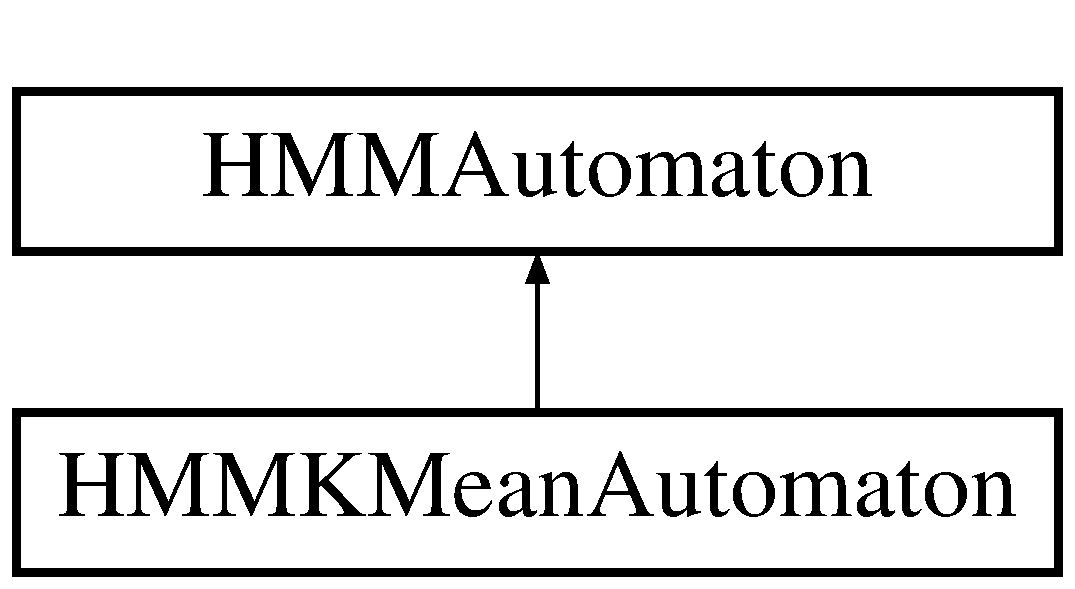
\includegraphics[height=2.000000cm]{class_h_m_m_k_mean_automaton}
\end{center}
\end{figure}
\subsection*{Public Member Functions}
\begin{DoxyCompactItemize}
\item 
\hyperlink{class_h_m_m_k_mean_automaton_a8a0788b8b6dabaecee663e15fca35d04}{H\+M\+M\+K\+Mean\+Automaton} (std\+::vector$<$ \hyperlink{class_wave_feature_o_p}{Wave\+Feature\+O\+P} $>$ $\ast$\hyperlink{class_h_m_m_automaton_a9932eb5aa8ff484ac2406f98498595cf}{templates}, int state\+Num=\hyperlink{configure__hmm_8h_aa9cc71cb42394379957677c761aae79e}{A\+U\+T\+O\+M\+A\+T\+O\+N\+\_\+\+S\+T\+A\+T\+E\+\_\+\+N\+U\+M}, int \hyperlink{pro6__demo_8cpp_a923ffcfa3c56ccdba17bc4e700247d54}{gauss\+Num}=\hyperlink{configure__hmm_8h_a8f9db0624fff0b17f641785bb8d66a82}{G\+A\+U\+S\+S\+I\+A\+N\+\_\+\+N\+U\+M}, int train\+Times=\hyperlink{configure__hmm_8h_a52e22519b5a37e58632e9183d5197b86}{M\+A\+X\+\_\+\+T\+R\+A\+I\+N\+\_\+\+T\+I\+M\+E\+S})
\item 
\hyperlink{class_h_m_m_k_mean_automaton_aff941d0dd58e9ca9bc5aad82f8e1f081}{$\sim$\+H\+M\+M\+K\+Mean\+Automaton} ()
\item 
void \hyperlink{class_h_m_m_k_mean_automaton_a1123c813c91a51bf9d2b9ad9043bbdf8}{hmm\+Train} ()
\item 
double \hyperlink{class_h_m_m_k_mean_automaton_a65df5f2b00684dc7dbfd14f5980ce5b9}{calc\+Cost} (\hyperlink{class_wave_feature_o_p}{Wave\+Feature\+O\+P} \&input)
\item 
void \hyperlink{class_h_m_m_k_mean_automaton_a9aecd65316ff521abed2ec0eb291f27a}{hmm\+Malloc\+States\+And\+Transfer} ()
\item 
void \hyperlink{class_h_m_m_k_mean_automaton_aa95d52fcb3f1e1ce6298e531d709e805}{hmm\+Initilize} ()
\item 
void \hyperlink{class_h_m_m_k_mean_automaton_a7986907c7fb6c7e94ab3e8e8739ff340}{iterate\+Gauss} ()
\item 
void \hyperlink{class_h_m_m_k_mean_automaton_a4c76f84ca4f618311d299a96f0877394}{init\+Segment} (int template\+Idx, int start\+I, int end\+I)
\item 
void \hyperlink{class_h_m_m_k_mean_automaton_a98247e299f3d9feb8ac2a13a1ad243f0}{init\+Transfer} ()
\item 
void \hyperlink{class_h_m_m_k_mean_automaton_a7b56f990d725bd0e8c872e71fb64989f}{all\+Empty\+State\+Segment} ()
\end{DoxyCompactItemize}
\subsection*{Private Member Functions}
\begin{DoxyCompactItemize}
\item 
\hyperlink{class_k_mean_state}{K\+Mean\+State} $\ast$ \hyperlink{class_h_m_m_k_mean_automaton_ac39190fc7bb62972d52deea3b20faabd}{get\+State} (int idx)
\item 
void \hyperlink{class_h_m_m_k_mean_automaton_a967fcfe7e5e00fd427df2d3f2ce313dc}{load} (std\+::stringstream \&in)
\item 
bool \hyperlink{class_h_m_m_k_mean_automaton_a0b85b69cc37eb2b0e373713a84f25f1a}{update\+Transfer} ()
\item 
void \hyperlink{class_h_m_m_k_mean_automaton_ab6430f6e5ed523fbd62b1954efed27ae}{update\+Segmentation} (int template\+Idx, int best\+Final\+Row\+Idx)
\item 
bool \hyperlink{class_h_m_m_k_mean_automaton_ada3475864afa9e258f2bd173d31acb34}{iterate\+Train} ()
\item 
void \hyperlink{class_h_m_m_k_mean_automaton_ae0b27687ddee80d49c8685175f095a8f}{clear\+Train\+Buffer} ()
\end{DoxyCompactItemize}
\subsection*{Friends}
\begin{DoxyCompactItemize}
\item 
class \hyperlink{class_h_m_m_k_mean_automaton_af469c501c992964354ce9cdaaf140d43}{H\+M\+M\+Seq\+K\+Mean\+Trainer}
\end{DoxyCompactItemize}
\subsection*{Additional Inherited Members}


\subsection{Constructor \& Destructor Documentation}
\hypertarget{class_h_m_m_k_mean_automaton_a8a0788b8b6dabaecee663e15fca35d04}{\index{H\+M\+M\+K\+Mean\+Automaton@{H\+M\+M\+K\+Mean\+Automaton}!H\+M\+M\+K\+Mean\+Automaton@{H\+M\+M\+K\+Mean\+Automaton}}
\index{H\+M\+M\+K\+Mean\+Automaton@{H\+M\+M\+K\+Mean\+Automaton}!H\+M\+M\+K\+Mean\+Automaton@{H\+M\+M\+K\+Mean\+Automaton}}
\subsubsection[{H\+M\+M\+K\+Mean\+Automaton}]{\setlength{\rightskip}{0pt plus 5cm}H\+M\+M\+K\+Mean\+Automaton\+::\+H\+M\+M\+K\+Mean\+Automaton (
\begin{DoxyParamCaption}
\item[{std\+::vector$<$ {\bf Wave\+Feature\+O\+P} $>$ $\ast$}]{templates, }
\item[{int}]{state\+Num = {\ttfamily {\bf A\+U\+T\+O\+M\+A\+T\+O\+N\+\_\+\+S\+T\+A\+T\+E\+\_\+\+N\+U\+M}}, }
\item[{int}]{gauss\+Num = {\ttfamily {\bf G\+A\+U\+S\+S\+I\+A\+N\+\_\+\+N\+U\+M}}, }
\item[{int}]{train\+Times = {\ttfamily {\bf M\+A\+X\+\_\+\+T\+R\+A\+I\+N\+\_\+\+T\+I\+M\+E\+S}}}
\end{DoxyParamCaption}
)}}\label{class_h_m_m_k_mean_automaton_a8a0788b8b6dabaecee663e15fca35d04}
\hypertarget{class_h_m_m_k_mean_automaton_aff941d0dd58e9ca9bc5aad82f8e1f081}{\index{H\+M\+M\+K\+Mean\+Automaton@{H\+M\+M\+K\+Mean\+Automaton}!````~H\+M\+M\+K\+Mean\+Automaton@{$\sim$\+H\+M\+M\+K\+Mean\+Automaton}}
\index{````~H\+M\+M\+K\+Mean\+Automaton@{$\sim$\+H\+M\+M\+K\+Mean\+Automaton}!H\+M\+M\+K\+Mean\+Automaton@{H\+M\+M\+K\+Mean\+Automaton}}
\subsubsection[{$\sim$\+H\+M\+M\+K\+Mean\+Automaton}]{\setlength{\rightskip}{0pt plus 5cm}H\+M\+M\+K\+Mean\+Automaton\+::$\sim$\+H\+M\+M\+K\+Mean\+Automaton (
\begin{DoxyParamCaption}
{}
\end{DoxyParamCaption}
)}}\label{class_h_m_m_k_mean_automaton_aff941d0dd58e9ca9bc5aad82f8e1f081}


\subsection{Member Function Documentation}
\hypertarget{class_h_m_m_k_mean_automaton_a7b56f990d725bd0e8c872e71fb64989f}{\index{H\+M\+M\+K\+Mean\+Automaton@{H\+M\+M\+K\+Mean\+Automaton}!all\+Empty\+State\+Segment@{all\+Empty\+State\+Segment}}
\index{all\+Empty\+State\+Segment@{all\+Empty\+State\+Segment}!H\+M\+M\+K\+Mean\+Automaton@{H\+M\+M\+K\+Mean\+Automaton}}
\subsubsection[{all\+Empty\+State\+Segment}]{\setlength{\rightskip}{0pt plus 5cm}void H\+M\+M\+K\+Mean\+Automaton\+::all\+Empty\+State\+Segment (
\begin{DoxyParamCaption}
{}
\end{DoxyParamCaption}
)}}\label{class_h_m_m_k_mean_automaton_a7b56f990d725bd0e8c872e71fb64989f}
\hypertarget{class_h_m_m_k_mean_automaton_a65df5f2b00684dc7dbfd14f5980ce5b9}{\index{H\+M\+M\+K\+Mean\+Automaton@{H\+M\+M\+K\+Mean\+Automaton}!calc\+Cost@{calc\+Cost}}
\index{calc\+Cost@{calc\+Cost}!H\+M\+M\+K\+Mean\+Automaton@{H\+M\+M\+K\+Mean\+Automaton}}
\subsubsection[{calc\+Cost}]{\setlength{\rightskip}{0pt plus 5cm}double H\+M\+M\+K\+Mean\+Automaton\+::calc\+Cost (
\begin{DoxyParamCaption}
\item[{{\bf Wave\+Feature\+O\+P} \&}]{input}
\end{DoxyParamCaption}
)\hspace{0.3cm}{\ttfamily [virtual]}}}\label{class_h_m_m_k_mean_automaton_a65df5f2b00684dc7dbfd14f5980ce5b9}


Implements \hyperlink{class_h_m_m_automaton_a4c43e2b6bba8c6f237bf4503d79b1f12}{H\+M\+M\+Automaton}.

\hypertarget{class_h_m_m_k_mean_automaton_ae0b27687ddee80d49c8685175f095a8f}{\index{H\+M\+M\+K\+Mean\+Automaton@{H\+M\+M\+K\+Mean\+Automaton}!clear\+Train\+Buffer@{clear\+Train\+Buffer}}
\index{clear\+Train\+Buffer@{clear\+Train\+Buffer}!H\+M\+M\+K\+Mean\+Automaton@{H\+M\+M\+K\+Mean\+Automaton}}
\subsubsection[{clear\+Train\+Buffer}]{\setlength{\rightskip}{0pt plus 5cm}void H\+M\+M\+K\+Mean\+Automaton\+::clear\+Train\+Buffer (
\begin{DoxyParamCaption}
{}
\end{DoxyParamCaption}
)\hspace{0.3cm}{\ttfamily [inline]}, {\ttfamily [private]}}}\label{class_h_m_m_k_mean_automaton_ae0b27687ddee80d49c8685175f095a8f}
\hypertarget{class_h_m_m_k_mean_automaton_ac39190fc7bb62972d52deea3b20faabd}{\index{H\+M\+M\+K\+Mean\+Automaton@{H\+M\+M\+K\+Mean\+Automaton}!get\+State@{get\+State}}
\index{get\+State@{get\+State}!H\+M\+M\+K\+Mean\+Automaton@{H\+M\+M\+K\+Mean\+Automaton}}
\subsubsection[{get\+State}]{\setlength{\rightskip}{0pt plus 5cm}{\bf K\+Mean\+State}$\ast$ H\+M\+M\+K\+Mean\+Automaton\+::get\+State (
\begin{DoxyParamCaption}
\item[{int}]{idx}
\end{DoxyParamCaption}
)\hspace{0.3cm}{\ttfamily [inline]}, {\ttfamily [private]}}}\label{class_h_m_m_k_mean_automaton_ac39190fc7bb62972d52deea3b20faabd}
\hypertarget{class_h_m_m_k_mean_automaton_aa95d52fcb3f1e1ce6298e531d709e805}{\index{H\+M\+M\+K\+Mean\+Automaton@{H\+M\+M\+K\+Mean\+Automaton}!hmm\+Initilize@{hmm\+Initilize}}
\index{hmm\+Initilize@{hmm\+Initilize}!H\+M\+M\+K\+Mean\+Automaton@{H\+M\+M\+K\+Mean\+Automaton}}
\subsubsection[{hmm\+Initilize}]{\setlength{\rightskip}{0pt plus 5cm}void H\+M\+M\+K\+Mean\+Automaton\+::hmm\+Initilize (
\begin{DoxyParamCaption}
{}
\end{DoxyParamCaption}
)}}\label{class_h_m_m_k_mean_automaton_aa95d52fcb3f1e1ce6298e531d709e805}
\hypertarget{class_h_m_m_k_mean_automaton_a9aecd65316ff521abed2ec0eb291f27a}{\index{H\+M\+M\+K\+Mean\+Automaton@{H\+M\+M\+K\+Mean\+Automaton}!hmm\+Malloc\+States\+And\+Transfer@{hmm\+Malloc\+States\+And\+Transfer}}
\index{hmm\+Malloc\+States\+And\+Transfer@{hmm\+Malloc\+States\+And\+Transfer}!H\+M\+M\+K\+Mean\+Automaton@{H\+M\+M\+K\+Mean\+Automaton}}
\subsubsection[{hmm\+Malloc\+States\+And\+Transfer}]{\setlength{\rightskip}{0pt plus 5cm}void H\+M\+M\+K\+Mean\+Automaton\+::hmm\+Malloc\+States\+And\+Transfer (
\begin{DoxyParamCaption}
{}
\end{DoxyParamCaption}
)}}\label{class_h_m_m_k_mean_automaton_a9aecd65316ff521abed2ec0eb291f27a}
\hypertarget{class_h_m_m_k_mean_automaton_a1123c813c91a51bf9d2b9ad9043bbdf8}{\index{H\+M\+M\+K\+Mean\+Automaton@{H\+M\+M\+K\+Mean\+Automaton}!hmm\+Train@{hmm\+Train}}
\index{hmm\+Train@{hmm\+Train}!H\+M\+M\+K\+Mean\+Automaton@{H\+M\+M\+K\+Mean\+Automaton}}
\subsubsection[{hmm\+Train}]{\setlength{\rightskip}{0pt plus 5cm}void H\+M\+M\+K\+Mean\+Automaton\+::hmm\+Train (
\begin{DoxyParamCaption}
{}
\end{DoxyParamCaption}
)\hspace{0.3cm}{\ttfamily [virtual]}}}\label{class_h_m_m_k_mean_automaton_a1123c813c91a51bf9d2b9ad9043bbdf8}


Implements \hyperlink{class_h_m_m_automaton_ac6bbc2770cb11b1c9e55cd0652fbe0e3}{H\+M\+M\+Automaton}.

\hypertarget{class_h_m_m_k_mean_automaton_a4c76f84ca4f618311d299a96f0877394}{\index{H\+M\+M\+K\+Mean\+Automaton@{H\+M\+M\+K\+Mean\+Automaton}!init\+Segment@{init\+Segment}}
\index{init\+Segment@{init\+Segment}!H\+M\+M\+K\+Mean\+Automaton@{H\+M\+M\+K\+Mean\+Automaton}}
\subsubsection[{init\+Segment}]{\setlength{\rightskip}{0pt plus 5cm}void H\+M\+M\+K\+Mean\+Automaton\+::init\+Segment (
\begin{DoxyParamCaption}
\item[{int}]{template\+Idx, }
\item[{int}]{start\+I, }
\item[{int}]{end\+I}
\end{DoxyParamCaption}
)}}\label{class_h_m_m_k_mean_automaton_a4c76f84ca4f618311d299a96f0877394}
\hypertarget{class_h_m_m_k_mean_automaton_a98247e299f3d9feb8ac2a13a1ad243f0}{\index{H\+M\+M\+K\+Mean\+Automaton@{H\+M\+M\+K\+Mean\+Automaton}!init\+Transfer@{init\+Transfer}}
\index{init\+Transfer@{init\+Transfer}!H\+M\+M\+K\+Mean\+Automaton@{H\+M\+M\+K\+Mean\+Automaton}}
\subsubsection[{init\+Transfer}]{\setlength{\rightskip}{0pt plus 5cm}void H\+M\+M\+K\+Mean\+Automaton\+::init\+Transfer (
\begin{DoxyParamCaption}
{}
\end{DoxyParamCaption}
)}}\label{class_h_m_m_k_mean_automaton_a98247e299f3d9feb8ac2a13a1ad243f0}
\hypertarget{class_h_m_m_k_mean_automaton_a7986907c7fb6c7e94ab3e8e8739ff340}{\index{H\+M\+M\+K\+Mean\+Automaton@{H\+M\+M\+K\+Mean\+Automaton}!iterate\+Gauss@{iterate\+Gauss}}
\index{iterate\+Gauss@{iterate\+Gauss}!H\+M\+M\+K\+Mean\+Automaton@{H\+M\+M\+K\+Mean\+Automaton}}
\subsubsection[{iterate\+Gauss}]{\setlength{\rightskip}{0pt plus 5cm}void H\+M\+M\+K\+Mean\+Automaton\+::iterate\+Gauss (
\begin{DoxyParamCaption}
{}
\end{DoxyParamCaption}
)}}\label{class_h_m_m_k_mean_automaton_a7986907c7fb6c7e94ab3e8e8739ff340}
\hypertarget{class_h_m_m_k_mean_automaton_ada3475864afa9e258f2bd173d31acb34}{\index{H\+M\+M\+K\+Mean\+Automaton@{H\+M\+M\+K\+Mean\+Automaton}!iterate\+Train@{iterate\+Train}}
\index{iterate\+Train@{iterate\+Train}!H\+M\+M\+K\+Mean\+Automaton@{H\+M\+M\+K\+Mean\+Automaton}}
\subsubsection[{iterate\+Train}]{\setlength{\rightskip}{0pt plus 5cm}bool H\+M\+M\+K\+Mean\+Automaton\+::iterate\+Train (
\begin{DoxyParamCaption}
{}
\end{DoxyParamCaption}
)\hspace{0.3cm}{\ttfamily [inline]}, {\ttfamily [private]}}}\label{class_h_m_m_k_mean_automaton_ada3475864afa9e258f2bd173d31acb34}
\hypertarget{class_h_m_m_k_mean_automaton_a967fcfe7e5e00fd427df2d3f2ce313dc}{\index{H\+M\+M\+K\+Mean\+Automaton@{H\+M\+M\+K\+Mean\+Automaton}!load@{load}}
\index{load@{load}!H\+M\+M\+K\+Mean\+Automaton@{H\+M\+M\+K\+Mean\+Automaton}}
\subsubsection[{load}]{\setlength{\rightskip}{0pt plus 5cm}void H\+M\+M\+K\+Mean\+Automaton\+::load (
\begin{DoxyParamCaption}
\item[{std\+::stringstream \&}]{in}
\end{DoxyParamCaption}
)\hspace{0.3cm}{\ttfamily [inline]}, {\ttfamily [private]}, {\ttfamily [virtual]}}}\label{class_h_m_m_k_mean_automaton_a967fcfe7e5e00fd427df2d3f2ce313dc}


Implements \hyperlink{class_h_m_m_automaton_a04b64e19e77d5fe8b78d471470346872}{H\+M\+M\+Automaton}.

\hypertarget{class_h_m_m_k_mean_automaton_ab6430f6e5ed523fbd62b1954efed27ae}{\index{H\+M\+M\+K\+Mean\+Automaton@{H\+M\+M\+K\+Mean\+Automaton}!update\+Segmentation@{update\+Segmentation}}
\index{update\+Segmentation@{update\+Segmentation}!H\+M\+M\+K\+Mean\+Automaton@{H\+M\+M\+K\+Mean\+Automaton}}
\subsubsection[{update\+Segmentation}]{\setlength{\rightskip}{0pt plus 5cm}void H\+M\+M\+K\+Mean\+Automaton\+::update\+Segmentation (
\begin{DoxyParamCaption}
\item[{int}]{template\+Idx, }
\item[{int}]{best\+Final\+Row\+Idx}
\end{DoxyParamCaption}
)\hspace{0.3cm}{\ttfamily [private]}}}\label{class_h_m_m_k_mean_automaton_ab6430f6e5ed523fbd62b1954efed27ae}
\hypertarget{class_h_m_m_k_mean_automaton_a0b85b69cc37eb2b0e373713a84f25f1a}{\index{H\+M\+M\+K\+Mean\+Automaton@{H\+M\+M\+K\+Mean\+Automaton}!update\+Transfer@{update\+Transfer}}
\index{update\+Transfer@{update\+Transfer}!H\+M\+M\+K\+Mean\+Automaton@{H\+M\+M\+K\+Mean\+Automaton}}
\subsubsection[{update\+Transfer}]{\setlength{\rightskip}{0pt plus 5cm}bool H\+M\+M\+K\+Mean\+Automaton\+::update\+Transfer (
\begin{DoxyParamCaption}
{}
\end{DoxyParamCaption}
)\hspace{0.3cm}{\ttfamily [private]}}}\label{class_h_m_m_k_mean_automaton_a0b85b69cc37eb2b0e373713a84f25f1a}


\subsection{Friends And Related Function Documentation}
\hypertarget{class_h_m_m_k_mean_automaton_af469c501c992964354ce9cdaaf140d43}{\index{H\+M\+M\+K\+Mean\+Automaton@{H\+M\+M\+K\+Mean\+Automaton}!H\+M\+M\+Seq\+K\+Mean\+Trainer@{H\+M\+M\+Seq\+K\+Mean\+Trainer}}
\index{H\+M\+M\+Seq\+K\+Mean\+Trainer@{H\+M\+M\+Seq\+K\+Mean\+Trainer}!H\+M\+M\+K\+Mean\+Automaton@{H\+M\+M\+K\+Mean\+Automaton}}
\subsubsection[{H\+M\+M\+Seq\+K\+Mean\+Trainer}]{\setlength{\rightskip}{0pt plus 5cm}friend class {\bf H\+M\+M\+Seq\+K\+Mean\+Trainer}\hspace{0.3cm}{\ttfamily [friend]}}}\label{class_h_m_m_k_mean_automaton_af469c501c992964354ce9cdaaf140d43}


The documentation for this class was generated from the following files\+:\begin{DoxyCompactItemize}
\item 
src/\+Feature/\hyperlink{_h_m_m_k_mean_automaton_8h}{H\+M\+M\+K\+Mean\+Automaton.\+h}\item 
src/\+Feature/\hyperlink{_h_m_m_kmean_automaton_8cpp}{H\+M\+M\+Kmean\+Automaton.\+cpp}\end{DoxyCompactItemize}

\hypertarget{class_h_m_m_recognition}{\section{H\+M\+M\+Recognition Class Reference}
\label{class_h_m_m_recognition}\index{H\+M\+M\+Recognition@{H\+M\+M\+Recognition}}
}


{\ttfamily \#include $<$H\+M\+M\+Recognition.\+h$>$}

Inheritance diagram for H\+M\+M\+Recognition\+:\begin{figure}[H]
\begin{center}
\leavevmode
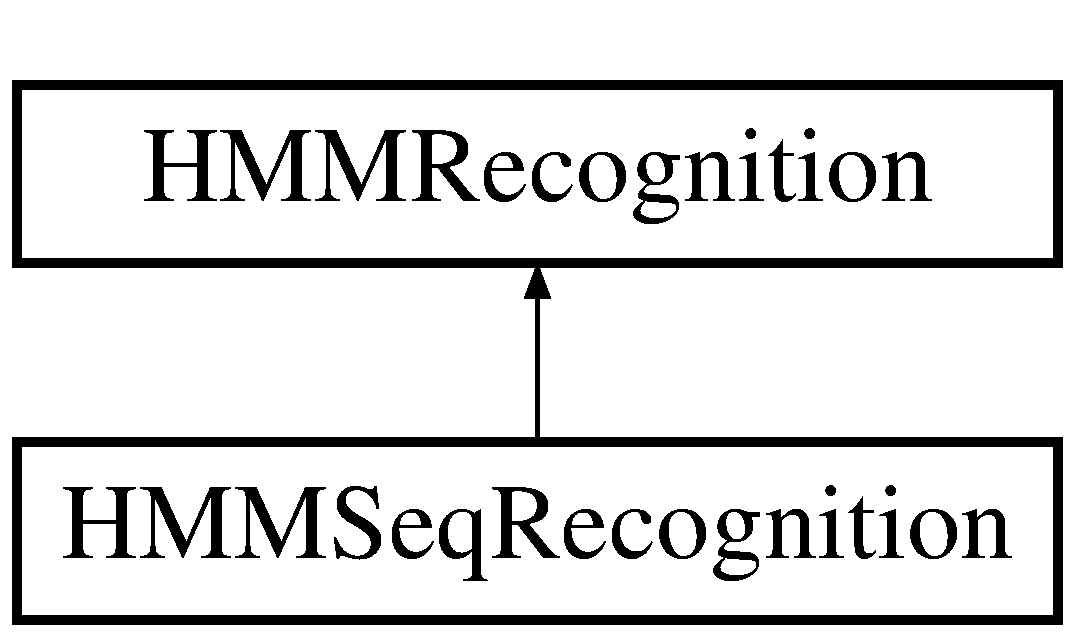
\includegraphics[height=2.000000cm]{class_h_m_m_recognition}
\end{center}
\end{figure}
\subsection*{Public Member Functions}
\begin{DoxyCompactItemize}
\item 
\hyperlink{class_h_m_m_recognition_a527df82050d6a04a9aa0be6498532feb}{H\+M\+M\+Recognition} (int \hyperlink{class_h_m_m_recognition_ac9be31139899e7e69694de527d229fd8}{state\+Num}=\hyperlink{configure__hmm_8h_aa9cc71cb42394379957677c761aae79e}{A\+U\+T\+O\+M\+A\+T\+O\+N\+\_\+\+S\+T\+A\+T\+E\+\_\+\+N\+U\+M}, int \hyperlink{class_h_m_m_recognition_af01765163d9d0092534231a20183b0e2}{gauss\+Num}=\hyperlink{configure__hmm_8h_a8f9db0624fff0b17f641785bb8d66a82}{G\+A\+U\+S\+S\+I\+A\+N\+\_\+\+N\+U\+M}, int \hyperlink{class_h_m_m_recognition_ad7bbe647d17214ad2b0de893bc03a8d5}{train\+Times}=\hyperlink{configure__hmm_8h_a52e22519b5a37e58632e9183d5197b86}{M\+A\+X\+\_\+\+T\+R\+A\+I\+N\+\_\+\+T\+I\+M\+E\+S})
\item 
virtual \hyperlink{class_h_m_m_recognition_a035b79783e60523afb4138b65be8692f}{$\sim$\+H\+M\+M\+Recognition} ()
\item 
\hyperlink{tool_8h_ab71a1f2fb85a32402ced5c483105b38e}{S\+P\+\_\+\+R\+E\+S\+U\+L\+T} \hyperlink{class_h_m_m_recognition_aceee222a2b4a3f6bbfe59e0a0fbe5e9b}{load\+Templates} (char $\ast$\hyperlink{class_h_m_m_recognition_ae665e0044a1a240b77ff84e877aa3170}{template\+Dir}, \hyperlink{class_wave_feature_o_p_abd93c85d1ed5fbc148d41b7f32fc1d84}{Wave\+Feature\+O\+P\+::\+L\+O\+A\+D\+\_\+\+T\+Y\+P\+E} load\+Type=\hyperlink{class_wave_feature_o_p_abd93c85d1ed5fbc148d41b7f32fc1d84a1b64a07dfde0c2d4132bc343f4475856}{Wave\+Feature\+O\+P\+::\+F\+U\+L\+L\+\_\+\+L\+O\+A\+D})
\item 
\hyperlink{tool_8h_ab71a1f2fb85a32402ced5c483105b38e}{S\+P\+\_\+\+R\+E\+S\+U\+L\+T} \hyperlink{class_h_m_m_recognition_a1bbccaae5aef122d97ae21589f7ced26}{hmm\+Train} (\hyperlink{class_h_m_m_automaton_aa3476c86db5e0791de6f07076f220348}{H\+M\+M\+Automaton\+::\+T\+R\+A\+I\+N\+\_\+\+T\+Y\+P\+E} \hyperlink{readhtk_8m_ac7798f4aec24aa6076b2b222bd91d4fd}{type}=\hyperlink{class_h_m_m_automaton_aa3476c86db5e0791de6f07076f220348a725fd42edf8b8e4b515b6296a7d67bb3}{H\+M\+M\+Automaton\+::\+S\+E\+G})
\item 
\hyperlink{tool_8h_ab71a1f2fb85a32402ced5c483105b38e}{S\+P\+\_\+\+R\+E\+S\+U\+L\+T} \hyperlink{class_h_m_m_recognition_a206cc7b9f0c2837c9773aa1f01bc4b93}{hmm\+Try\+Load} (char $\ast$\hyperlink{class_h_m_m_recognition_ae665e0044a1a240b77ff84e877aa3170}{template\+Dir})
\item 
virtual std\+::string \hyperlink{class_h_m_m_recognition_a5f583004dd3281ab1375539258d4c6f7}{hmm\+Recognition} (\hyperlink{class_wave_feature_o_p}{Wave\+Feature\+O\+P} \&input)
\item 
virtual void \hyperlink{class_h_m_m_recognition_ae373459e832f7d1bf13730ee255dbd92}{close} ()
\item 
void \hyperlink{class_h_m_m_recognition_a77996d0232da91730e848775b2d99f3e}{set\+State\+Num} (int \hyperlink{class_h_m_m_recognition_ac9be31139899e7e69694de527d229fd8}{state\+Num})
\item 
void \hyperlink{class_h_m_m_recognition_acdf125127b3d655b56ce222407bb3fed}{set\+Gauss\+Num} (int \hyperlink{class_h_m_m_recognition_af01765163d9d0092534231a20183b0e2}{gauss\+Num})
\item 
void \hyperlink{class_h_m_m_recognition_a71575bab89514444b3d280182aacf6f9}{set\+Train\+Times} (int \hyperlink{class_h_m_m_recognition_ad7bbe647d17214ad2b0de893bc03a8d5}{train\+Times})
\item 
void \hyperlink{class_h_m_m_recognition_a8c0bb4205e8b3fde6c905fb17019263f}{dump\+Automaton} (std\+::ostream \&out)
\end{DoxyCompactItemize}
\subsection*{Protected Member Functions}
\begin{DoxyCompactItemize}
\item 
bool \hyperlink{class_h_m_m_recognition_a7968c6ec0f7af2efa1173aafb72bf1a2}{load\+H\+M\+M\+Model} ()
\item 
void \hyperlink{class_h_m_m_recognition_a6929deeda71a27dc403e421bd530f21b}{store\+H\+M\+M\+Model} ()
\item 
string \hyperlink{class_h_m_m_recognition_a30450b0cb477359a2c6f8e9a85910b40}{generate\+H\+M\+M\+File\+Name} ()
\end{DoxyCompactItemize}
\subsection*{Protected Attributes}
\begin{DoxyCompactItemize}
\item 
int \hyperlink{class_h_m_m_recognition_ac9be31139899e7e69694de527d229fd8}{state\+Num}
\item 
int \hyperlink{class_h_m_m_recognition_af01765163d9d0092534231a20183b0e2}{gauss\+Num}
\item 
int \hyperlink{class_h_m_m_recognition_ad7bbe647d17214ad2b0de893bc03a8d5}{train\+Times}
\item 
string \hyperlink{class_h_m_m_recognition_ae665e0044a1a240b77ff84e877aa3170}{template\+Dir}
\item 
\hyperlink{class_h_m_m_automaton_set}{H\+M\+M\+Automaton\+Set} \hyperlink{class_h_m_m_recognition_a28bd7824ff0afaf5a712f3ef4149f52f}{automatons}
\end{DoxyCompactItemize}
\subsection*{Private Member Functions}
\begin{DoxyCompactItemize}
\item 
\hyperlink{class_h_m_m_recognition_a1b9e6a926d9f15771eed5061ae67af87}{R\+E\+A\+D\+\_\+\+W\+R\+I\+T\+E\+\_\+\+D\+E\+C\+L\+A\+R\+E} (\hyperlink{class_h_m_m_state_a35d2a059c2410a52110329b637940046}{H\+M\+M\+State\+::\+State\+Type}, state\+Type, State\+Type)
\end{DoxyCompactItemize}


\subsection{Constructor \& Destructor Documentation}
\hypertarget{class_h_m_m_recognition_a527df82050d6a04a9aa0be6498532feb}{\index{H\+M\+M\+Recognition@{H\+M\+M\+Recognition}!H\+M\+M\+Recognition@{H\+M\+M\+Recognition}}
\index{H\+M\+M\+Recognition@{H\+M\+M\+Recognition}!H\+M\+M\+Recognition@{H\+M\+M\+Recognition}}
\subsubsection[{H\+M\+M\+Recognition}]{\setlength{\rightskip}{0pt plus 5cm}H\+M\+M\+Recognition\+::\+H\+M\+M\+Recognition (
\begin{DoxyParamCaption}
\item[{int}]{state\+Num = {\ttfamily {\bf A\+U\+T\+O\+M\+A\+T\+O\+N\+\_\+\+S\+T\+A\+T\+E\+\_\+\+N\+U\+M}}, }
\item[{int}]{gauss\+Num = {\ttfamily {\bf G\+A\+U\+S\+S\+I\+A\+N\+\_\+\+N\+U\+M}}, }
\item[{int}]{train\+Times = {\ttfamily {\bf M\+A\+X\+\_\+\+T\+R\+A\+I\+N\+\_\+\+T\+I\+M\+E\+S}}}
\end{DoxyParamCaption}
)}}\label{class_h_m_m_recognition_a527df82050d6a04a9aa0be6498532feb}
\hypertarget{class_h_m_m_recognition_a035b79783e60523afb4138b65be8692f}{\index{H\+M\+M\+Recognition@{H\+M\+M\+Recognition}!````~H\+M\+M\+Recognition@{$\sim$\+H\+M\+M\+Recognition}}
\index{````~H\+M\+M\+Recognition@{$\sim$\+H\+M\+M\+Recognition}!H\+M\+M\+Recognition@{H\+M\+M\+Recognition}}
\subsubsection[{$\sim$\+H\+M\+M\+Recognition}]{\setlength{\rightskip}{0pt plus 5cm}H\+M\+M\+Recognition\+::$\sim$\+H\+M\+M\+Recognition (
\begin{DoxyParamCaption}
{}
\end{DoxyParamCaption}
)\hspace{0.3cm}{\ttfamily [virtual]}}}\label{class_h_m_m_recognition_a035b79783e60523afb4138b65be8692f}


\subsection{Member Function Documentation}
\hypertarget{class_h_m_m_recognition_ae373459e832f7d1bf13730ee255dbd92}{\index{H\+M\+M\+Recognition@{H\+M\+M\+Recognition}!close@{close}}
\index{close@{close}!H\+M\+M\+Recognition@{H\+M\+M\+Recognition}}
\subsubsection[{close}]{\setlength{\rightskip}{0pt plus 5cm}void H\+M\+M\+Recognition\+::close (
\begin{DoxyParamCaption}
{}
\end{DoxyParamCaption}
)\hspace{0.3cm}{\ttfamily [virtual]}}}\label{class_h_m_m_recognition_ae373459e832f7d1bf13730ee255dbd92}


Reimplemented in \hyperlink{class_h_m_m_seq_recognition_aab6f8979a62075758b12cb097f3dc03a}{H\+M\+M\+Seq\+Recognition}.

\hypertarget{class_h_m_m_recognition_a8c0bb4205e8b3fde6c905fb17019263f}{\index{H\+M\+M\+Recognition@{H\+M\+M\+Recognition}!dump\+Automaton@{dump\+Automaton}}
\index{dump\+Automaton@{dump\+Automaton}!H\+M\+M\+Recognition@{H\+M\+M\+Recognition}}
\subsubsection[{dump\+Automaton}]{\setlength{\rightskip}{0pt plus 5cm}void H\+M\+M\+Recognition\+::dump\+Automaton (
\begin{DoxyParamCaption}
\item[{std\+::ostream \&}]{out}
\end{DoxyParamCaption}
)}}\label{class_h_m_m_recognition_a8c0bb4205e8b3fde6c905fb17019263f}
\hypertarget{class_h_m_m_recognition_a30450b0cb477359a2c6f8e9a85910b40}{\index{H\+M\+M\+Recognition@{H\+M\+M\+Recognition}!generate\+H\+M\+M\+File\+Name@{generate\+H\+M\+M\+File\+Name}}
\index{generate\+H\+M\+M\+File\+Name@{generate\+H\+M\+M\+File\+Name}!H\+M\+M\+Recognition@{H\+M\+M\+Recognition}}
\subsubsection[{generate\+H\+M\+M\+File\+Name}]{\setlength{\rightskip}{0pt plus 5cm}string H\+M\+M\+Recognition\+::generate\+H\+M\+M\+File\+Name (
\begin{DoxyParamCaption}
{}
\end{DoxyParamCaption}
)\hspace{0.3cm}{\ttfamily [protected]}}}\label{class_h_m_m_recognition_a30450b0cb477359a2c6f8e9a85910b40}
\hypertarget{class_h_m_m_recognition_a5f583004dd3281ab1375539258d4c6f7}{\index{H\+M\+M\+Recognition@{H\+M\+M\+Recognition}!hmm\+Recognition@{hmm\+Recognition}}
\index{hmm\+Recognition@{hmm\+Recognition}!H\+M\+M\+Recognition@{H\+M\+M\+Recognition}}
\subsubsection[{hmm\+Recognition}]{\setlength{\rightskip}{0pt plus 5cm}std\+::string H\+M\+M\+Recognition\+::hmm\+Recognition (
\begin{DoxyParamCaption}
\item[{{\bf Wave\+Feature\+O\+P} \&}]{input}
\end{DoxyParamCaption}
)\hspace{0.3cm}{\ttfamily [virtual]}}}\label{class_h_m_m_recognition_a5f583004dd3281ab1375539258d4c6f7}
\hypertarget{class_h_m_m_recognition_a1bbccaae5aef122d97ae21589f7ced26}{\index{H\+M\+M\+Recognition@{H\+M\+M\+Recognition}!hmm\+Train@{hmm\+Train}}
\index{hmm\+Train@{hmm\+Train}!H\+M\+M\+Recognition@{H\+M\+M\+Recognition}}
\subsubsection[{hmm\+Train}]{\setlength{\rightskip}{0pt plus 5cm}{\bf S\+P\+\_\+\+R\+E\+S\+U\+L\+T} H\+M\+M\+Recognition\+::hmm\+Train (
\begin{DoxyParamCaption}
\item[{{\bf H\+M\+M\+Automaton\+::\+T\+R\+A\+I\+N\+\_\+\+T\+Y\+P\+E}}]{type = {\ttfamily {\bf H\+M\+M\+Automaton\+::\+S\+E\+G}}}
\end{DoxyParamCaption}
)}}\label{class_h_m_m_recognition_a1bbccaae5aef122d97ae21589f7ced26}
\hypertarget{class_h_m_m_recognition_a206cc7b9f0c2837c9773aa1f01bc4b93}{\index{H\+M\+M\+Recognition@{H\+M\+M\+Recognition}!hmm\+Try\+Load@{hmm\+Try\+Load}}
\index{hmm\+Try\+Load@{hmm\+Try\+Load}!H\+M\+M\+Recognition@{H\+M\+M\+Recognition}}
\subsubsection[{hmm\+Try\+Load}]{\setlength{\rightskip}{0pt plus 5cm}{\bf S\+P\+\_\+\+R\+E\+S\+U\+L\+T} H\+M\+M\+Recognition\+::hmm\+Try\+Load (
\begin{DoxyParamCaption}
\item[{char $\ast$}]{template\+Dir}
\end{DoxyParamCaption}
)}}\label{class_h_m_m_recognition_a206cc7b9f0c2837c9773aa1f01bc4b93}
\hypertarget{class_h_m_m_recognition_a7968c6ec0f7af2efa1173aafb72bf1a2}{\index{H\+M\+M\+Recognition@{H\+M\+M\+Recognition}!load\+H\+M\+M\+Model@{load\+H\+M\+M\+Model}}
\index{load\+H\+M\+M\+Model@{load\+H\+M\+M\+Model}!H\+M\+M\+Recognition@{H\+M\+M\+Recognition}}
\subsubsection[{load\+H\+M\+M\+Model}]{\setlength{\rightskip}{0pt plus 5cm}bool H\+M\+M\+Recognition\+::load\+H\+M\+M\+Model (
\begin{DoxyParamCaption}
{}
\end{DoxyParamCaption}
)\hspace{0.3cm}{\ttfamily [protected]}}}\label{class_h_m_m_recognition_a7968c6ec0f7af2efa1173aafb72bf1a2}
\hypertarget{class_h_m_m_recognition_aceee222a2b4a3f6bbfe59e0a0fbe5e9b}{\index{H\+M\+M\+Recognition@{H\+M\+M\+Recognition}!load\+Templates@{load\+Templates}}
\index{load\+Templates@{load\+Templates}!H\+M\+M\+Recognition@{H\+M\+M\+Recognition}}
\subsubsection[{load\+Templates}]{\setlength{\rightskip}{0pt plus 5cm}{\bf S\+P\+\_\+\+R\+E\+S\+U\+L\+T} H\+M\+M\+Recognition\+::load\+Templates (
\begin{DoxyParamCaption}
\item[{char $\ast$}]{template\+Dir, }
\item[{{\bf Wave\+Feature\+O\+P\+::\+L\+O\+A\+D\+\_\+\+T\+Y\+P\+E}}]{load\+Type = {\ttfamily {\bf Wave\+Feature\+O\+P\+::\+F\+U\+L\+L\+\_\+\+L\+O\+A\+D}}}
\end{DoxyParamCaption}
)}}\label{class_h_m_m_recognition_aceee222a2b4a3f6bbfe59e0a0fbe5e9b}
\hypertarget{class_h_m_m_recognition_a1b9e6a926d9f15771eed5061ae67af87}{\index{H\+M\+M\+Recognition@{H\+M\+M\+Recognition}!R\+E\+A\+D\+\_\+\+W\+R\+I\+T\+E\+\_\+\+D\+E\+C\+L\+A\+R\+E@{R\+E\+A\+D\+\_\+\+W\+R\+I\+T\+E\+\_\+\+D\+E\+C\+L\+A\+R\+E}}
\index{R\+E\+A\+D\+\_\+\+W\+R\+I\+T\+E\+\_\+\+D\+E\+C\+L\+A\+R\+E@{R\+E\+A\+D\+\_\+\+W\+R\+I\+T\+E\+\_\+\+D\+E\+C\+L\+A\+R\+E}!H\+M\+M\+Recognition@{H\+M\+M\+Recognition}}
\subsubsection[{R\+E\+A\+D\+\_\+\+W\+R\+I\+T\+E\+\_\+\+D\+E\+C\+L\+A\+R\+E}]{\setlength{\rightskip}{0pt plus 5cm}H\+M\+M\+Recognition\+::\+R\+E\+A\+D\+\_\+\+W\+R\+I\+T\+E\+\_\+\+D\+E\+C\+L\+A\+R\+E (
\begin{DoxyParamCaption}
\item[{{\bf H\+M\+M\+State\+::\+State\+Type}}]{, }
\item[{state\+Type}]{, }
\item[{State\+Type}]{}
\end{DoxyParamCaption}
)\hspace{0.3cm}{\ttfamily [private]}}}\label{class_h_m_m_recognition_a1b9e6a926d9f15771eed5061ae67af87}
\hypertarget{class_h_m_m_recognition_acdf125127b3d655b56ce222407bb3fed}{\index{H\+M\+M\+Recognition@{H\+M\+M\+Recognition}!set\+Gauss\+Num@{set\+Gauss\+Num}}
\index{set\+Gauss\+Num@{set\+Gauss\+Num}!H\+M\+M\+Recognition@{H\+M\+M\+Recognition}}
\subsubsection[{set\+Gauss\+Num}]{\setlength{\rightskip}{0pt plus 5cm}void H\+M\+M\+Recognition\+::set\+Gauss\+Num (
\begin{DoxyParamCaption}
\item[{int}]{gauss\+Num}
\end{DoxyParamCaption}
)\hspace{0.3cm}{\ttfamily [inline]}}}\label{class_h_m_m_recognition_acdf125127b3d655b56ce222407bb3fed}
\hypertarget{class_h_m_m_recognition_a77996d0232da91730e848775b2d99f3e}{\index{H\+M\+M\+Recognition@{H\+M\+M\+Recognition}!set\+State\+Num@{set\+State\+Num}}
\index{set\+State\+Num@{set\+State\+Num}!H\+M\+M\+Recognition@{H\+M\+M\+Recognition}}
\subsubsection[{set\+State\+Num}]{\setlength{\rightskip}{0pt plus 5cm}void H\+M\+M\+Recognition\+::set\+State\+Num (
\begin{DoxyParamCaption}
\item[{int}]{state\+Num}
\end{DoxyParamCaption}
)\hspace{0.3cm}{\ttfamily [inline]}}}\label{class_h_m_m_recognition_a77996d0232da91730e848775b2d99f3e}
\hypertarget{class_h_m_m_recognition_a71575bab89514444b3d280182aacf6f9}{\index{H\+M\+M\+Recognition@{H\+M\+M\+Recognition}!set\+Train\+Times@{set\+Train\+Times}}
\index{set\+Train\+Times@{set\+Train\+Times}!H\+M\+M\+Recognition@{H\+M\+M\+Recognition}}
\subsubsection[{set\+Train\+Times}]{\setlength{\rightskip}{0pt plus 5cm}void H\+M\+M\+Recognition\+::set\+Train\+Times (
\begin{DoxyParamCaption}
\item[{int}]{train\+Times}
\end{DoxyParamCaption}
)\hspace{0.3cm}{\ttfamily [inline]}}}\label{class_h_m_m_recognition_a71575bab89514444b3d280182aacf6f9}
\hypertarget{class_h_m_m_recognition_a6929deeda71a27dc403e421bd530f21b}{\index{H\+M\+M\+Recognition@{H\+M\+M\+Recognition}!store\+H\+M\+M\+Model@{store\+H\+M\+M\+Model}}
\index{store\+H\+M\+M\+Model@{store\+H\+M\+M\+Model}!H\+M\+M\+Recognition@{H\+M\+M\+Recognition}}
\subsubsection[{store\+H\+M\+M\+Model}]{\setlength{\rightskip}{0pt plus 5cm}void H\+M\+M\+Recognition\+::store\+H\+M\+M\+Model (
\begin{DoxyParamCaption}
{}
\end{DoxyParamCaption}
)\hspace{0.3cm}{\ttfamily [protected]}}}\label{class_h_m_m_recognition_a6929deeda71a27dc403e421bd530f21b}


\subsection{Member Data Documentation}
\hypertarget{class_h_m_m_recognition_a28bd7824ff0afaf5a712f3ef4149f52f}{\index{H\+M\+M\+Recognition@{H\+M\+M\+Recognition}!automatons@{automatons}}
\index{automatons@{automatons}!H\+M\+M\+Recognition@{H\+M\+M\+Recognition}}
\subsubsection[{automatons}]{\setlength{\rightskip}{0pt plus 5cm}{\bf H\+M\+M\+Automaton\+Set} H\+M\+M\+Recognition\+::automatons\hspace{0.3cm}{\ttfamily [protected]}}}\label{class_h_m_m_recognition_a28bd7824ff0afaf5a712f3ef4149f52f}
\hypertarget{class_h_m_m_recognition_af01765163d9d0092534231a20183b0e2}{\index{H\+M\+M\+Recognition@{H\+M\+M\+Recognition}!gauss\+Num@{gauss\+Num}}
\index{gauss\+Num@{gauss\+Num}!H\+M\+M\+Recognition@{H\+M\+M\+Recognition}}
\subsubsection[{gauss\+Num}]{\setlength{\rightskip}{0pt plus 5cm}int H\+M\+M\+Recognition\+::gauss\+Num\hspace{0.3cm}{\ttfamily [protected]}}}\label{class_h_m_m_recognition_af01765163d9d0092534231a20183b0e2}
\hypertarget{class_h_m_m_recognition_ac9be31139899e7e69694de527d229fd8}{\index{H\+M\+M\+Recognition@{H\+M\+M\+Recognition}!state\+Num@{state\+Num}}
\index{state\+Num@{state\+Num}!H\+M\+M\+Recognition@{H\+M\+M\+Recognition}}
\subsubsection[{state\+Num}]{\setlength{\rightskip}{0pt plus 5cm}int H\+M\+M\+Recognition\+::state\+Num\hspace{0.3cm}{\ttfamily [protected]}}}\label{class_h_m_m_recognition_ac9be31139899e7e69694de527d229fd8}
\hypertarget{class_h_m_m_recognition_ae665e0044a1a240b77ff84e877aa3170}{\index{H\+M\+M\+Recognition@{H\+M\+M\+Recognition}!template\+Dir@{template\+Dir}}
\index{template\+Dir@{template\+Dir}!H\+M\+M\+Recognition@{H\+M\+M\+Recognition}}
\subsubsection[{template\+Dir}]{\setlength{\rightskip}{0pt plus 5cm}string H\+M\+M\+Recognition\+::template\+Dir\hspace{0.3cm}{\ttfamily [protected]}}}\label{class_h_m_m_recognition_ae665e0044a1a240b77ff84e877aa3170}
\hypertarget{class_h_m_m_recognition_ad7bbe647d17214ad2b0de893bc03a8d5}{\index{H\+M\+M\+Recognition@{H\+M\+M\+Recognition}!train\+Times@{train\+Times}}
\index{train\+Times@{train\+Times}!H\+M\+M\+Recognition@{H\+M\+M\+Recognition}}
\subsubsection[{train\+Times}]{\setlength{\rightskip}{0pt plus 5cm}int H\+M\+M\+Recognition\+::train\+Times\hspace{0.3cm}{\ttfamily [protected]}}}\label{class_h_m_m_recognition_ad7bbe647d17214ad2b0de893bc03a8d5}


The documentation for this class was generated from the following files\+:\begin{DoxyCompactItemize}
\item 
src/\+Feature/\hyperlink{_h_m_m_recognition_8h}{H\+M\+M\+Recognition.\+h}\item 
src/\+Feature/\hyperlink{_h_m_m_recognition_8cpp}{H\+M\+M\+Recognition.\+cpp}\end{DoxyCompactItemize}

\hypertarget{class_h_m_m_seq_k_mean_trainer}{\section{H\+M\+M\+Seq\+K\+Mean\+Trainer Class Reference}
\label{class_h_m_m_seq_k_mean_trainer}\index{H\+M\+M\+Seq\+K\+Mean\+Trainer@{H\+M\+M\+Seq\+K\+Mean\+Trainer}}
}


{\ttfamily \#include $<$H\+M\+M\+Seq\+K\+Mean\+Trainer.\+h$>$}

Inheritance diagram for H\+M\+M\+Seq\+K\+Mean\+Trainer\+:\begin{figure}[H]
\begin{center}
\leavevmode
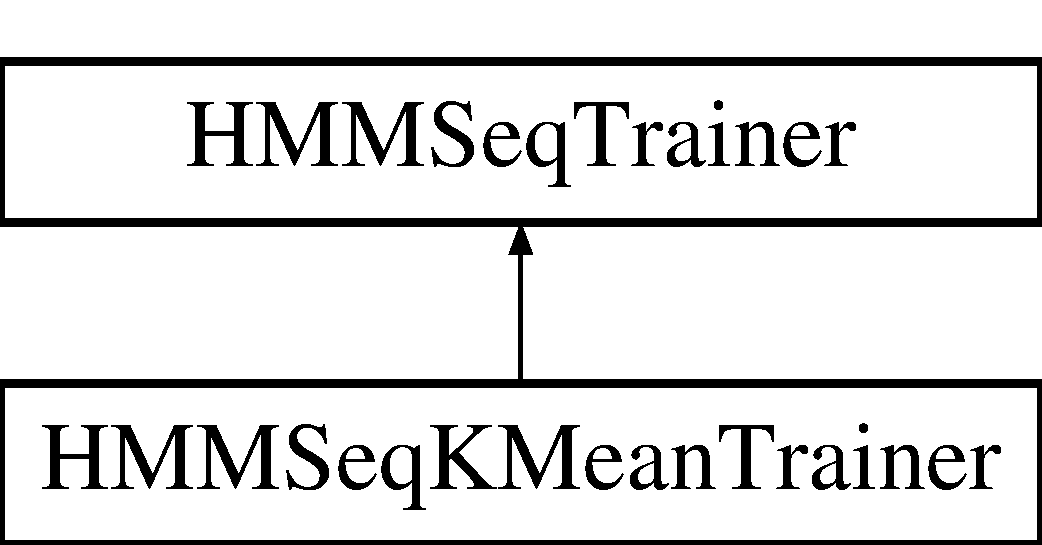
\includegraphics[height=2.000000cm]{class_h_m_m_seq_k_mean_trainer}
\end{center}
\end{figure}
\subsection*{Public Member Functions}
\begin{DoxyCompactItemize}
\item 
\hyperlink{class_h_m_m_seq_k_mean_trainer_a783eaefd9b12b2df1d7fdc2cb15713b6}{H\+M\+M\+Seq\+K\+Mean\+Trainer} ()
\item 
\hyperlink{class_h_m_m_seq_k_mean_trainer_a42591784f7b48776a3ac5542a62b8d46}{$\sim$\+H\+M\+M\+Seq\+K\+Mean\+Trainer} ()
\end{DoxyCompactItemize}
\subsection*{Private Member Functions}
\begin{DoxyCompactItemize}
\item 
void \hyperlink{class_h_m_m_seq_k_mean_trainer_a0d76c424f623667cff7ec0262d06f172}{hmm\+Seq\+Train} ()
\item 
void \hyperlink{class_h_m_m_seq_k_mean_trainer_aeb81a388b2d8070cdba12e911826101e}{init\+H\+M\+M\+Train} ()
\item 
bool \hyperlink{class_h_m_m_seq_k_mean_trainer_a988cda8fc52326b3aef67a2c6b91588b}{iterator\+Seq\+Train} ()
\end{DoxyCompactItemize}
\subsection*{Additional Inherited Members}


\subsection{Constructor \& Destructor Documentation}
\hypertarget{class_h_m_m_seq_k_mean_trainer_a783eaefd9b12b2df1d7fdc2cb15713b6}{\index{H\+M\+M\+Seq\+K\+Mean\+Trainer@{H\+M\+M\+Seq\+K\+Mean\+Trainer}!H\+M\+M\+Seq\+K\+Mean\+Trainer@{H\+M\+M\+Seq\+K\+Mean\+Trainer}}
\index{H\+M\+M\+Seq\+K\+Mean\+Trainer@{H\+M\+M\+Seq\+K\+Mean\+Trainer}!H\+M\+M\+Seq\+K\+Mean\+Trainer@{H\+M\+M\+Seq\+K\+Mean\+Trainer}}
\subsubsection[{H\+M\+M\+Seq\+K\+Mean\+Trainer}]{\setlength{\rightskip}{0pt plus 5cm}H\+M\+M\+Seq\+K\+Mean\+Trainer\+::\+H\+M\+M\+Seq\+K\+Mean\+Trainer (
\begin{DoxyParamCaption}
{}
\end{DoxyParamCaption}
)}}\label{class_h_m_m_seq_k_mean_trainer_a783eaefd9b12b2df1d7fdc2cb15713b6}
\hypertarget{class_h_m_m_seq_k_mean_trainer_a42591784f7b48776a3ac5542a62b8d46}{\index{H\+M\+M\+Seq\+K\+Mean\+Trainer@{H\+M\+M\+Seq\+K\+Mean\+Trainer}!````~H\+M\+M\+Seq\+K\+Mean\+Trainer@{$\sim$\+H\+M\+M\+Seq\+K\+Mean\+Trainer}}
\index{````~H\+M\+M\+Seq\+K\+Mean\+Trainer@{$\sim$\+H\+M\+M\+Seq\+K\+Mean\+Trainer}!H\+M\+M\+Seq\+K\+Mean\+Trainer@{H\+M\+M\+Seq\+K\+Mean\+Trainer}}
\subsubsection[{$\sim$\+H\+M\+M\+Seq\+K\+Mean\+Trainer}]{\setlength{\rightskip}{0pt plus 5cm}H\+M\+M\+Seq\+K\+Mean\+Trainer\+::$\sim$\+H\+M\+M\+Seq\+K\+Mean\+Trainer (
\begin{DoxyParamCaption}
{}
\end{DoxyParamCaption}
)}}\label{class_h_m_m_seq_k_mean_trainer_a42591784f7b48776a3ac5542a62b8d46}


\subsection{Member Function Documentation}
\hypertarget{class_h_m_m_seq_k_mean_trainer_a0d76c424f623667cff7ec0262d06f172}{\index{H\+M\+M\+Seq\+K\+Mean\+Trainer@{H\+M\+M\+Seq\+K\+Mean\+Trainer}!hmm\+Seq\+Train@{hmm\+Seq\+Train}}
\index{hmm\+Seq\+Train@{hmm\+Seq\+Train}!H\+M\+M\+Seq\+K\+Mean\+Trainer@{H\+M\+M\+Seq\+K\+Mean\+Trainer}}
\subsubsection[{hmm\+Seq\+Train}]{\setlength{\rightskip}{0pt plus 5cm}void H\+M\+M\+Seq\+K\+Mean\+Trainer\+::hmm\+Seq\+Train (
\begin{DoxyParamCaption}
{}
\end{DoxyParamCaption}
)\hspace{0.3cm}{\ttfamily [private]}, {\ttfamily [virtual]}}}\label{class_h_m_m_seq_k_mean_trainer_a0d76c424f623667cff7ec0262d06f172}


Implements \hyperlink{class_h_m_m_seq_trainer_a72dcee91292fba79b652518b7ea8c8d5}{H\+M\+M\+Seq\+Trainer}.

\hypertarget{class_h_m_m_seq_k_mean_trainer_aeb81a388b2d8070cdba12e911826101e}{\index{H\+M\+M\+Seq\+K\+Mean\+Trainer@{H\+M\+M\+Seq\+K\+Mean\+Trainer}!init\+H\+M\+M\+Train@{init\+H\+M\+M\+Train}}
\index{init\+H\+M\+M\+Train@{init\+H\+M\+M\+Train}!H\+M\+M\+Seq\+K\+Mean\+Trainer@{H\+M\+M\+Seq\+K\+Mean\+Trainer}}
\subsubsection[{init\+H\+M\+M\+Train}]{\setlength{\rightskip}{0pt plus 5cm}void H\+M\+M\+Seq\+K\+Mean\+Trainer\+::init\+H\+M\+M\+Train (
\begin{DoxyParamCaption}
{}
\end{DoxyParamCaption}
)\hspace{0.3cm}{\ttfamily [private]}}}\label{class_h_m_m_seq_k_mean_trainer_aeb81a388b2d8070cdba12e911826101e}
\hypertarget{class_h_m_m_seq_k_mean_trainer_a988cda8fc52326b3aef67a2c6b91588b}{\index{H\+M\+M\+Seq\+K\+Mean\+Trainer@{H\+M\+M\+Seq\+K\+Mean\+Trainer}!iterator\+Seq\+Train@{iterator\+Seq\+Train}}
\index{iterator\+Seq\+Train@{iterator\+Seq\+Train}!H\+M\+M\+Seq\+K\+Mean\+Trainer@{H\+M\+M\+Seq\+K\+Mean\+Trainer}}
\subsubsection[{iterator\+Seq\+Train}]{\setlength{\rightskip}{0pt plus 5cm}bool H\+M\+M\+Seq\+K\+Mean\+Trainer\+::iterator\+Seq\+Train (
\begin{DoxyParamCaption}
{}
\end{DoxyParamCaption}
)\hspace{0.3cm}{\ttfamily [private]}}}\label{class_h_m_m_seq_k_mean_trainer_a988cda8fc52326b3aef67a2c6b91588b}


The documentation for this class was generated from the following files\+:\begin{DoxyCompactItemize}
\item 
src/\+Feature/\hyperlink{_h_m_m_seq_k_mean_trainer_8h}{H\+M\+M\+Seq\+K\+Mean\+Trainer.\+h}\item 
src/\+Feature/\hyperlink{_h_m_m_seq_k_mean_trainer_8cpp}{H\+M\+M\+Seq\+K\+Mean\+Trainer.\+cpp}\end{DoxyCompactItemize}

\hypertarget{class_h_m_m_seq_recognition}{\section{H\+M\+M\+Seq\+Recognition Class Reference}
\label{class_h_m_m_seq_recognition}\index{H\+M\+M\+Seq\+Recognition@{H\+M\+M\+Seq\+Recognition}}
}


{\ttfamily \#include $<$H\+M\+M\+Seq\+Recognition.\+h$>$}

Inheritance diagram for H\+M\+M\+Seq\+Recognition\+:\begin{figure}[H]
\begin{center}
\leavevmode
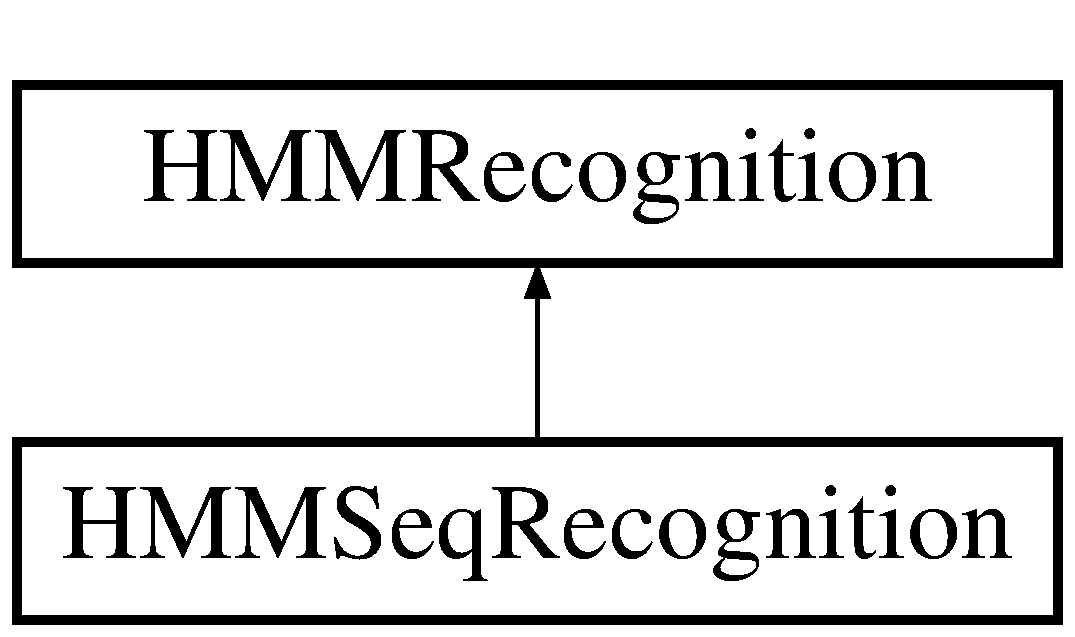
\includegraphics[height=2.000000cm]{class_h_m_m_seq_recognition}
\end{center}
\end{figure}
\subsection*{Public Member Functions}
\begin{DoxyCompactItemize}
\item 
\hyperlink{class_h_m_m_seq_recognition_ad31375206b98b00a23053eafc6fa4acb}{H\+M\+M\+Seq\+Recognition} (int \hyperlink{class_h_m_m_recognition_ac9be31139899e7e69694de527d229fd8}{state\+Num}=\hyperlink{configure__hmm_8h_aa9cc71cb42394379957677c761aae79e}{A\+U\+T\+O\+M\+A\+T\+O\+N\+\_\+\+S\+T\+A\+T\+E\+\_\+\+N\+U\+M}, int \hyperlink{class_h_m_m_recognition_af01765163d9d0092534231a20183b0e2}{gauss\+Num}=\hyperlink{configure__hmm_8h_a8f9db0624fff0b17f641785bb8d66a82}{G\+A\+U\+S\+S\+I\+A\+N\+\_\+\+N\+U\+M}, int \hyperlink{class_h_m_m_recognition_ad7bbe647d17214ad2b0de893bc03a8d5}{train\+Times}=\hyperlink{configure__hmm_8h_a52e22519b5a37e58632e9183d5197b86}{M\+A\+X\+\_\+\+T\+R\+A\+I\+N\+\_\+\+T\+I\+M\+E\+S})
\item 
\hyperlink{class_h_m_m_seq_recognition_a8a140fd37bc6136e736e4a18af468c24}{$\sim$\+H\+M\+M\+Seq\+Recognition} ()
\item 
void \hyperlink{class_h_m_m_seq_recognition_aa7fde29aff2eedb94bb348286e81755e}{hmm\+Seg\+Train} ()
\item 
void \hyperlink{class_h_m_m_seq_recognition_a4aacbb864b59fab32a5179b29d5dc697}{hmm\+Seq\+Train} ()
\item 
void \hyperlink{class_h_m_m_seq_recognition_a6f9d60d3b76b0206908d2d3489c7a74f}{load\+Graph} (const char $\ast$filename)
\item 
void \hyperlink{class_h_m_m_seq_recognition_a6d1e4941efc0412cc91e64598786163b}{recognition} (\hyperlink{class_wave_feature_o_p}{Wave\+Feature\+O\+P} \&input, std\+::vector$<$ std\+::string $>$ \&res, \hyperlink{class_seq_model_a145b769692f03811a15c5289fe77da42}{Seq\+Model\+::\+S\+E\+Q\+\_\+\+D\+T\+W\+\_\+\+P\+A\+T\+H\+\_\+\+T\+Y\+P\+E} \hyperlink{pro6__demo_8cpp_a3741bb1053b40df849a053be5cca6a7a}{path\+Type}=\hyperlink{class_seq_model_a145b769692f03811a15c5289fe77da42a4e15f646c0c498e155c24f183dbfb6fb}{Seq\+Model\+::\+B\+A\+C\+K\+\_\+\+P\+T\+R})
\item 
void \hyperlink{class_h_m_m_seq_recognition_a9b318a686915464ebdc29ff3beff846e}{set\+Beam} (double beam)
\item 
void \hyperlink{class_h_m_m_seq_recognition_a41681a169988cb857642fcabdf0ecf1d}{dump\+Dot} (std\+::ofstream \&out)
\item 
void \hyperlink{class_h_m_m_seq_recognition_aab6f8979a62075758b12cb097f3dc03a}{close} ()
\end{DoxyCompactItemize}
\subsection*{Private Member Functions}
\begin{DoxyCompactItemize}
\item 
void \hyperlink{class_h_m_m_seq_recognition_afe35a34d7f03bb857683f0db7e0593a8}{build\+Seq\+Model} ()
\end{DoxyCompactItemize}
\subsection*{Private Attributes}
\begin{DoxyCompactItemize}
\item 
\hyperlink{class_parse_graph}{Parse\+Graph} \hyperlink{class_h_m_m_seq_recognition_a7102c5c76a993fd7ecaa84398c5fc524}{graph}
\item 
\hyperlink{class_seq_model}{Seq\+Model} \hyperlink{class_h_m_m_seq_recognition_a36ede5e827ea9429c0997ef78726941f}{seq\+Model}
\end{DoxyCompactItemize}
\subsection*{Additional Inherited Members}


\subsection{Constructor \& Destructor Documentation}
\hypertarget{class_h_m_m_seq_recognition_ad31375206b98b00a23053eafc6fa4acb}{\index{H\+M\+M\+Seq\+Recognition@{H\+M\+M\+Seq\+Recognition}!H\+M\+M\+Seq\+Recognition@{H\+M\+M\+Seq\+Recognition}}
\index{H\+M\+M\+Seq\+Recognition@{H\+M\+M\+Seq\+Recognition}!H\+M\+M\+Seq\+Recognition@{H\+M\+M\+Seq\+Recognition}}
\subsubsection[{H\+M\+M\+Seq\+Recognition}]{\setlength{\rightskip}{0pt plus 5cm}H\+M\+M\+Seq\+Recognition\+::\+H\+M\+M\+Seq\+Recognition (
\begin{DoxyParamCaption}
\item[{int}]{state\+Num = {\ttfamily {\bf A\+U\+T\+O\+M\+A\+T\+O\+N\+\_\+\+S\+T\+A\+T\+E\+\_\+\+N\+U\+M}}, }
\item[{int}]{gauss\+Num = {\ttfamily {\bf G\+A\+U\+S\+S\+I\+A\+N\+\_\+\+N\+U\+M}}, }
\item[{int}]{train\+Times = {\ttfamily {\bf M\+A\+X\+\_\+\+T\+R\+A\+I\+N\+\_\+\+T\+I\+M\+E\+S}}}
\end{DoxyParamCaption}
)}}\label{class_h_m_m_seq_recognition_ad31375206b98b00a23053eafc6fa4acb}
\hypertarget{class_h_m_m_seq_recognition_a8a140fd37bc6136e736e4a18af468c24}{\index{H\+M\+M\+Seq\+Recognition@{H\+M\+M\+Seq\+Recognition}!````~H\+M\+M\+Seq\+Recognition@{$\sim$\+H\+M\+M\+Seq\+Recognition}}
\index{````~H\+M\+M\+Seq\+Recognition@{$\sim$\+H\+M\+M\+Seq\+Recognition}!H\+M\+M\+Seq\+Recognition@{H\+M\+M\+Seq\+Recognition}}
\subsubsection[{$\sim$\+H\+M\+M\+Seq\+Recognition}]{\setlength{\rightskip}{0pt plus 5cm}H\+M\+M\+Seq\+Recognition\+::$\sim$\+H\+M\+M\+Seq\+Recognition (
\begin{DoxyParamCaption}
{}
\end{DoxyParamCaption}
)}}\label{class_h_m_m_seq_recognition_a8a140fd37bc6136e736e4a18af468c24}


\subsection{Member Function Documentation}
\hypertarget{class_h_m_m_seq_recognition_afe35a34d7f03bb857683f0db7e0593a8}{\index{H\+M\+M\+Seq\+Recognition@{H\+M\+M\+Seq\+Recognition}!build\+Seq\+Model@{build\+Seq\+Model}}
\index{build\+Seq\+Model@{build\+Seq\+Model}!H\+M\+M\+Seq\+Recognition@{H\+M\+M\+Seq\+Recognition}}
\subsubsection[{build\+Seq\+Model}]{\setlength{\rightskip}{0pt plus 5cm}void H\+M\+M\+Seq\+Recognition\+::build\+Seq\+Model (
\begin{DoxyParamCaption}
{}
\end{DoxyParamCaption}
)\hspace{0.3cm}{\ttfamily [private]}}}\label{class_h_m_m_seq_recognition_afe35a34d7f03bb857683f0db7e0593a8}
\hypertarget{class_h_m_m_seq_recognition_aab6f8979a62075758b12cb097f3dc03a}{\index{H\+M\+M\+Seq\+Recognition@{H\+M\+M\+Seq\+Recognition}!close@{close}}
\index{close@{close}!H\+M\+M\+Seq\+Recognition@{H\+M\+M\+Seq\+Recognition}}
\subsubsection[{close}]{\setlength{\rightskip}{0pt plus 5cm}void H\+M\+M\+Seq\+Recognition\+::close (
\begin{DoxyParamCaption}
{}
\end{DoxyParamCaption}
)\hspace{0.3cm}{\ttfamily [virtual]}}}\label{class_h_m_m_seq_recognition_aab6f8979a62075758b12cb097f3dc03a}


Reimplemented from \hyperlink{class_h_m_m_recognition_ae373459e832f7d1bf13730ee255dbd92}{H\+M\+M\+Recognition}.

\hypertarget{class_h_m_m_seq_recognition_a41681a169988cb857642fcabdf0ecf1d}{\index{H\+M\+M\+Seq\+Recognition@{H\+M\+M\+Seq\+Recognition}!dump\+Dot@{dump\+Dot}}
\index{dump\+Dot@{dump\+Dot}!H\+M\+M\+Seq\+Recognition@{H\+M\+M\+Seq\+Recognition}}
\subsubsection[{dump\+Dot}]{\setlength{\rightskip}{0pt plus 5cm}void H\+M\+M\+Seq\+Recognition\+::dump\+Dot (
\begin{DoxyParamCaption}
\item[{std\+::ofstream \&}]{out}
\end{DoxyParamCaption}
)}}\label{class_h_m_m_seq_recognition_a41681a169988cb857642fcabdf0ecf1d}
\hypertarget{class_h_m_m_seq_recognition_aa7fde29aff2eedb94bb348286e81755e}{\index{H\+M\+M\+Seq\+Recognition@{H\+M\+M\+Seq\+Recognition}!hmm\+Seg\+Train@{hmm\+Seg\+Train}}
\index{hmm\+Seg\+Train@{hmm\+Seg\+Train}!H\+M\+M\+Seq\+Recognition@{H\+M\+M\+Seq\+Recognition}}
\subsubsection[{hmm\+Seg\+Train}]{\setlength{\rightskip}{0pt plus 5cm}void H\+M\+M\+Seq\+Recognition\+::hmm\+Seg\+Train (
\begin{DoxyParamCaption}
{}
\end{DoxyParamCaption}
)}}\label{class_h_m_m_seq_recognition_aa7fde29aff2eedb94bb348286e81755e}
\hypertarget{class_h_m_m_seq_recognition_a4aacbb864b59fab32a5179b29d5dc697}{\index{H\+M\+M\+Seq\+Recognition@{H\+M\+M\+Seq\+Recognition}!hmm\+Seq\+Train@{hmm\+Seq\+Train}}
\index{hmm\+Seq\+Train@{hmm\+Seq\+Train}!H\+M\+M\+Seq\+Recognition@{H\+M\+M\+Seq\+Recognition}}
\subsubsection[{hmm\+Seq\+Train}]{\setlength{\rightskip}{0pt plus 5cm}void H\+M\+M\+Seq\+Recognition\+::hmm\+Seq\+Train (
\begin{DoxyParamCaption}
{}
\end{DoxyParamCaption}
)}}\label{class_h_m_m_seq_recognition_a4aacbb864b59fab32a5179b29d5dc697}
\hypertarget{class_h_m_m_seq_recognition_a6f9d60d3b76b0206908d2d3489c7a74f}{\index{H\+M\+M\+Seq\+Recognition@{H\+M\+M\+Seq\+Recognition}!load\+Graph@{load\+Graph}}
\index{load\+Graph@{load\+Graph}!H\+M\+M\+Seq\+Recognition@{H\+M\+M\+Seq\+Recognition}}
\subsubsection[{load\+Graph}]{\setlength{\rightskip}{0pt plus 5cm}void H\+M\+M\+Seq\+Recognition\+::load\+Graph (
\begin{DoxyParamCaption}
\item[{const char $\ast$}]{filename}
\end{DoxyParamCaption}
)}}\label{class_h_m_m_seq_recognition_a6f9d60d3b76b0206908d2d3489c7a74f}
\hypertarget{class_h_m_m_seq_recognition_a6d1e4941efc0412cc91e64598786163b}{\index{H\+M\+M\+Seq\+Recognition@{H\+M\+M\+Seq\+Recognition}!recognition@{recognition}}
\index{recognition@{recognition}!H\+M\+M\+Seq\+Recognition@{H\+M\+M\+Seq\+Recognition}}
\subsubsection[{recognition}]{\setlength{\rightskip}{0pt plus 5cm}void H\+M\+M\+Seq\+Recognition\+::recognition (
\begin{DoxyParamCaption}
\item[{{\bf Wave\+Feature\+O\+P} \&}]{input, }
\item[{std\+::vector$<$ std\+::string $>$ \&}]{res, }
\item[{{\bf Seq\+Model\+::\+S\+E\+Q\+\_\+\+D\+T\+W\+\_\+\+P\+A\+T\+H\+\_\+\+T\+Y\+P\+E}}]{path\+Type = {\ttfamily {\bf Seq\+Model\+::\+B\+A\+C\+K\+\_\+\+P\+T\+R}}}
\end{DoxyParamCaption}
)}}\label{class_h_m_m_seq_recognition_a6d1e4941efc0412cc91e64598786163b}
\hypertarget{class_h_m_m_seq_recognition_a9b318a686915464ebdc29ff3beff846e}{\index{H\+M\+M\+Seq\+Recognition@{H\+M\+M\+Seq\+Recognition}!set\+Beam@{set\+Beam}}
\index{set\+Beam@{set\+Beam}!H\+M\+M\+Seq\+Recognition@{H\+M\+M\+Seq\+Recognition}}
\subsubsection[{set\+Beam}]{\setlength{\rightskip}{0pt plus 5cm}void H\+M\+M\+Seq\+Recognition\+::set\+Beam (
\begin{DoxyParamCaption}
\item[{double}]{beam}
\end{DoxyParamCaption}
)}}\label{class_h_m_m_seq_recognition_a9b318a686915464ebdc29ff3beff846e}


\subsection{Member Data Documentation}
\hypertarget{class_h_m_m_seq_recognition_a7102c5c76a993fd7ecaa84398c5fc524}{\index{H\+M\+M\+Seq\+Recognition@{H\+M\+M\+Seq\+Recognition}!graph@{graph}}
\index{graph@{graph}!H\+M\+M\+Seq\+Recognition@{H\+M\+M\+Seq\+Recognition}}
\subsubsection[{graph}]{\setlength{\rightskip}{0pt plus 5cm}{\bf Parse\+Graph} H\+M\+M\+Seq\+Recognition\+::graph\hspace{0.3cm}{\ttfamily [private]}}}\label{class_h_m_m_seq_recognition_a7102c5c76a993fd7ecaa84398c5fc524}
\hypertarget{class_h_m_m_seq_recognition_a36ede5e827ea9429c0997ef78726941f}{\index{H\+M\+M\+Seq\+Recognition@{H\+M\+M\+Seq\+Recognition}!seq\+Model@{seq\+Model}}
\index{seq\+Model@{seq\+Model}!H\+M\+M\+Seq\+Recognition@{H\+M\+M\+Seq\+Recognition}}
\subsubsection[{seq\+Model}]{\setlength{\rightskip}{0pt plus 5cm}{\bf Seq\+Model} H\+M\+M\+Seq\+Recognition\+::seq\+Model\hspace{0.3cm}{\ttfamily [private]}}}\label{class_h_m_m_seq_recognition_a36ede5e827ea9429c0997ef78726941f}


The documentation for this class was generated from the following files\+:\begin{DoxyCompactItemize}
\item 
src/\+Feature/\hyperlink{_h_m_m_seq_recognition_8h}{H\+M\+M\+Seq\+Recognition.\+h}\item 
src/\+Feature/\hyperlink{_h_m_m_seq_recognition_8cpp}{H\+M\+M\+Seq\+Recognition.\+cpp}\end{DoxyCompactItemize}

\hypertarget{class_h_m_m_seq_trainer}{\section{H\+M\+M\+Seq\+Trainer Class Reference}
\label{class_h_m_m_seq_trainer}\index{H\+M\+M\+Seq\+Trainer@{H\+M\+M\+Seq\+Trainer}}
}


{\ttfamily \#include $<$H\+M\+M\+Seq\+Trainer.\+h$>$}

Inheritance diagram for H\+M\+M\+Seq\+Trainer\+:\begin{figure}[H]
\begin{center}
\leavevmode
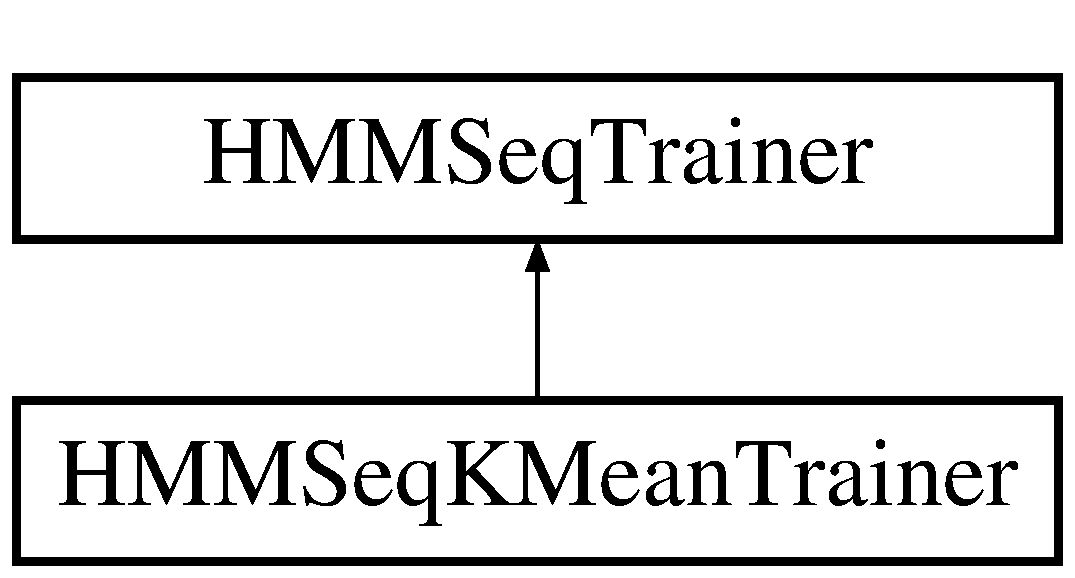
\includegraphics[height=2.000000cm]{class_h_m_m_seq_trainer}
\end{center}
\end{figure}
\subsection*{Public Member Functions}
\begin{DoxyCompactItemize}
\item 
\hyperlink{class_h_m_m_seq_trainer_a7057cd2041fd9a458b1f8e8f930bcaf8}{H\+M\+M\+Seq\+Trainer} ()
\item 
virtual \hyperlink{class_h_m_m_seq_trainer_ade6cb6a33af96d8f610276f86bceee09}{$\sim$\+H\+M\+M\+Seq\+Trainer} ()
\item 
void \hyperlink{class_h_m_m_seq_trainer_a391d1fe69c103b901cabc4c8d44d652c}{build\+Models} (\hyperlink{class_wave_feature_o_p_set_a7145e9463a1fb85ce4c239552bf4e8e0}{Wave\+Feature\+O\+P\+Set\+::data\+Set\+Type} \&data\+Set, std\+::map$<$ std\+::string, \hyperlink{class_h_m_m_automaton}{H\+M\+M\+Automaton} $\ast$ $>$ \&\hyperlink{class_h_m_m_seq_trainer_a70439ad48e64f17d74cdc968effb467f}{automatons}, std\+::vector$<$ \hyperlink{class_wave_feature_o_p}{Wave\+Feature\+O\+P} $>$ \&\hyperlink{class_h_m_m_seq_trainer_a74e6e47e0a794b07e0971cc482ebb5b3}{mixed\+Wavs})
\end{DoxyCompactItemize}
\subsection*{Protected Member Functions}
\begin{DoxyCompactItemize}
\item 
void \hyperlink{class_h_m_m_seq_trainer_afad2c364fd24e88b8e52ceb75c5c602f}{refresh\+Models} ()
\item 
void \hyperlink{class_h_m_m_seq_trainer_a494bbd7510d5f64683c7da573f74c25e}{build\+Models} ()
\end{DoxyCompactItemize}
\subsection*{Protected Attributes}
\begin{DoxyCompactItemize}
\item 
std\+::map$<$ std\+::string, \\*
\hyperlink{class_h_m_m_automaton}{H\+M\+M\+Automaton} $\ast$ $>$ $\ast$ \hyperlink{class_h_m_m_seq_trainer_a70439ad48e64f17d74cdc968effb467f}{automatons}
\item 
std\+::vector$<$ \hyperlink{class_h_m_m_automaton}{H\+M\+M\+Automaton} $\ast$ $>$ \hyperlink{class_h_m_m_seq_trainer_adbd7d13034cdf37f36bc8918f2b2b966}{automaton\+Vec}
\item 
std\+::vector$<$ \hyperlink{class_wave_feature_o_p}{Wave\+Feature\+O\+P} $>$ $\ast$ \hyperlink{class_h_m_m_seq_trainer_a74e6e47e0a794b07e0971cc482ebb5b3}{mixed\+Wavs}
\item 
std\+::vector$<$ \hyperlink{class_seq_model}{Seq\+Model} $>$ \hyperlink{class_h_m_m_seq_trainer_ac8e9e38eaab0a2d2bbb7e4770edc2c60}{train\+Models}
\item 
std\+::vector$<$ \hyperlink{class_parse_graph}{Parse\+Graph} $>$ \hyperlink{class_h_m_m_seq_trainer_a26beb77bab1fd38efa19cd4122f07c01}{graphs}
\item 
std\+::vector$<$ \hyperlink{struct_seq_wav}{Seq\+Wav} $>$ \hyperlink{class_h_m_m_seq_trainer_a290cfb899d17941cb6aba292f1a36e13}{train\+Wavs}
\end{DoxyCompactItemize}
\subsection*{Private Member Functions}
\begin{DoxyCompactItemize}
\item 
void \hyperlink{class_h_m_m_seq_trainer_ac1617cd69e1ca19075428bb4eddf1135}{push\+New\+Model} (const std\+::string \&seq\+Str, std\+::map$<$ std\+::string, \hyperlink{class_h_m_m_automaton}{H\+M\+M\+Automaton} $\ast$ $>$ \&\hyperlink{class_h_m_m_seq_trainer_a70439ad48e64f17d74cdc968effb467f}{automatons}, std\+::vector$<$ \hyperlink{class_seq_model}{Seq\+Model} $>$ \&models)
\item 
virtual void \hyperlink{class_h_m_m_seq_trainer_a72dcee91292fba79b652518b7ea8c8d5}{hmm\+Seq\+Train} ()=0
\end{DoxyCompactItemize}


\subsection{Constructor \& Destructor Documentation}
\hypertarget{class_h_m_m_seq_trainer_a7057cd2041fd9a458b1f8e8f930bcaf8}{\index{H\+M\+M\+Seq\+Trainer@{H\+M\+M\+Seq\+Trainer}!H\+M\+M\+Seq\+Trainer@{H\+M\+M\+Seq\+Trainer}}
\index{H\+M\+M\+Seq\+Trainer@{H\+M\+M\+Seq\+Trainer}!H\+M\+M\+Seq\+Trainer@{H\+M\+M\+Seq\+Trainer}}
\subsubsection[{H\+M\+M\+Seq\+Trainer}]{\setlength{\rightskip}{0pt plus 5cm}H\+M\+M\+Seq\+Trainer\+::\+H\+M\+M\+Seq\+Trainer (
\begin{DoxyParamCaption}
{}
\end{DoxyParamCaption}
)}}\label{class_h_m_m_seq_trainer_a7057cd2041fd9a458b1f8e8f930bcaf8}
\hypertarget{class_h_m_m_seq_trainer_ade6cb6a33af96d8f610276f86bceee09}{\index{H\+M\+M\+Seq\+Trainer@{H\+M\+M\+Seq\+Trainer}!````~H\+M\+M\+Seq\+Trainer@{$\sim$\+H\+M\+M\+Seq\+Trainer}}
\index{````~H\+M\+M\+Seq\+Trainer@{$\sim$\+H\+M\+M\+Seq\+Trainer}!H\+M\+M\+Seq\+Trainer@{H\+M\+M\+Seq\+Trainer}}
\subsubsection[{$\sim$\+H\+M\+M\+Seq\+Trainer}]{\setlength{\rightskip}{0pt plus 5cm}H\+M\+M\+Seq\+Trainer\+::$\sim$\+H\+M\+M\+Seq\+Trainer (
\begin{DoxyParamCaption}
{}
\end{DoxyParamCaption}
)\hspace{0.3cm}{\ttfamily [virtual]}}}\label{class_h_m_m_seq_trainer_ade6cb6a33af96d8f610276f86bceee09}


\subsection{Member Function Documentation}
\hypertarget{class_h_m_m_seq_trainer_a391d1fe69c103b901cabc4c8d44d652c}{\index{H\+M\+M\+Seq\+Trainer@{H\+M\+M\+Seq\+Trainer}!build\+Models@{build\+Models}}
\index{build\+Models@{build\+Models}!H\+M\+M\+Seq\+Trainer@{H\+M\+M\+Seq\+Trainer}}
\subsubsection[{build\+Models}]{\setlength{\rightskip}{0pt plus 5cm}void H\+M\+M\+Seq\+Trainer\+::build\+Models (
\begin{DoxyParamCaption}
\item[{{\bf Wave\+Feature\+O\+P\+Set\+::data\+Set\+Type} \&}]{data\+Set, }
\item[{std\+::map$<$ std\+::string, {\bf H\+M\+M\+Automaton} $\ast$ $>$ \&}]{automatons, }
\item[{std\+::vector$<$ {\bf Wave\+Feature\+O\+P} $>$ \&}]{mixed\+Wavs}
\end{DoxyParamCaption}
)}}\label{class_h_m_m_seq_trainer_a391d1fe69c103b901cabc4c8d44d652c}
\hypertarget{class_h_m_m_seq_trainer_a494bbd7510d5f64683c7da573f74c25e}{\index{H\+M\+M\+Seq\+Trainer@{H\+M\+M\+Seq\+Trainer}!build\+Models@{build\+Models}}
\index{build\+Models@{build\+Models}!H\+M\+M\+Seq\+Trainer@{H\+M\+M\+Seq\+Trainer}}
\subsubsection[{build\+Models}]{\setlength{\rightskip}{0pt plus 5cm}void H\+M\+M\+Seq\+Trainer\+::build\+Models (
\begin{DoxyParamCaption}
{}
\end{DoxyParamCaption}
)\hspace{0.3cm}{\ttfamily [protected]}}}\label{class_h_m_m_seq_trainer_a494bbd7510d5f64683c7da573f74c25e}
\hypertarget{class_h_m_m_seq_trainer_a72dcee91292fba79b652518b7ea8c8d5}{\index{H\+M\+M\+Seq\+Trainer@{H\+M\+M\+Seq\+Trainer}!hmm\+Seq\+Train@{hmm\+Seq\+Train}}
\index{hmm\+Seq\+Train@{hmm\+Seq\+Train}!H\+M\+M\+Seq\+Trainer@{H\+M\+M\+Seq\+Trainer}}
\subsubsection[{hmm\+Seq\+Train}]{\setlength{\rightskip}{0pt plus 5cm}virtual void H\+M\+M\+Seq\+Trainer\+::hmm\+Seq\+Train (
\begin{DoxyParamCaption}
{}
\end{DoxyParamCaption}
)\hspace{0.3cm}{\ttfamily [private]}, {\ttfamily [pure virtual]}}}\label{class_h_m_m_seq_trainer_a72dcee91292fba79b652518b7ea8c8d5}


Implemented in \hyperlink{class_h_m_m_seq_k_mean_trainer_a0d76c424f623667cff7ec0262d06f172}{H\+M\+M\+Seq\+K\+Mean\+Trainer}.

\hypertarget{class_h_m_m_seq_trainer_ac1617cd69e1ca19075428bb4eddf1135}{\index{H\+M\+M\+Seq\+Trainer@{H\+M\+M\+Seq\+Trainer}!push\+New\+Model@{push\+New\+Model}}
\index{push\+New\+Model@{push\+New\+Model}!H\+M\+M\+Seq\+Trainer@{H\+M\+M\+Seq\+Trainer}}
\subsubsection[{push\+New\+Model}]{\setlength{\rightskip}{0pt plus 5cm}void H\+M\+M\+Seq\+Trainer\+::push\+New\+Model (
\begin{DoxyParamCaption}
\item[{const std\+::string \&}]{seq\+Str, }
\item[{std\+::map$<$ std\+::string, {\bf H\+M\+M\+Automaton} $\ast$ $>$ \&}]{automatons, }
\item[{std\+::vector$<$ {\bf Seq\+Model} $>$ \&}]{models}
\end{DoxyParamCaption}
)\hspace{0.3cm}{\ttfamily [private]}}}\label{class_h_m_m_seq_trainer_ac1617cd69e1ca19075428bb4eddf1135}
\hypertarget{class_h_m_m_seq_trainer_afad2c364fd24e88b8e52ceb75c5c602f}{\index{H\+M\+M\+Seq\+Trainer@{H\+M\+M\+Seq\+Trainer}!refresh\+Models@{refresh\+Models}}
\index{refresh\+Models@{refresh\+Models}!H\+M\+M\+Seq\+Trainer@{H\+M\+M\+Seq\+Trainer}}
\subsubsection[{refresh\+Models}]{\setlength{\rightskip}{0pt plus 5cm}void H\+M\+M\+Seq\+Trainer\+::refresh\+Models (
\begin{DoxyParamCaption}
{}
\end{DoxyParamCaption}
)\hspace{0.3cm}{\ttfamily [protected]}}}\label{class_h_m_m_seq_trainer_afad2c364fd24e88b8e52ceb75c5c602f}


\subsection{Member Data Documentation}
\hypertarget{class_h_m_m_seq_trainer_a70439ad48e64f17d74cdc968effb467f}{\index{H\+M\+M\+Seq\+Trainer@{H\+M\+M\+Seq\+Trainer}!automatons@{automatons}}
\index{automatons@{automatons}!H\+M\+M\+Seq\+Trainer@{H\+M\+M\+Seq\+Trainer}}
\subsubsection[{automatons}]{\setlength{\rightskip}{0pt plus 5cm}std\+::map$<$std\+::string, {\bf H\+M\+M\+Automaton} $\ast$$>$$\ast$ H\+M\+M\+Seq\+Trainer\+::automatons\hspace{0.3cm}{\ttfamily [protected]}}}\label{class_h_m_m_seq_trainer_a70439ad48e64f17d74cdc968effb467f}
\hypertarget{class_h_m_m_seq_trainer_adbd7d13034cdf37f36bc8918f2b2b966}{\index{H\+M\+M\+Seq\+Trainer@{H\+M\+M\+Seq\+Trainer}!automaton\+Vec@{automaton\+Vec}}
\index{automaton\+Vec@{automaton\+Vec}!H\+M\+M\+Seq\+Trainer@{H\+M\+M\+Seq\+Trainer}}
\subsubsection[{automaton\+Vec}]{\setlength{\rightskip}{0pt plus 5cm}std\+::vector$<$ {\bf H\+M\+M\+Automaton} $\ast$$>$ H\+M\+M\+Seq\+Trainer\+::automaton\+Vec\hspace{0.3cm}{\ttfamily [protected]}}}\label{class_h_m_m_seq_trainer_adbd7d13034cdf37f36bc8918f2b2b966}
\hypertarget{class_h_m_m_seq_trainer_a26beb77bab1fd38efa19cd4122f07c01}{\index{H\+M\+M\+Seq\+Trainer@{H\+M\+M\+Seq\+Trainer}!graphs@{graphs}}
\index{graphs@{graphs}!H\+M\+M\+Seq\+Trainer@{H\+M\+M\+Seq\+Trainer}}
\subsubsection[{graphs}]{\setlength{\rightskip}{0pt plus 5cm}std\+::vector$<${\bf Parse\+Graph}$>$ H\+M\+M\+Seq\+Trainer\+::graphs\hspace{0.3cm}{\ttfamily [protected]}}}\label{class_h_m_m_seq_trainer_a26beb77bab1fd38efa19cd4122f07c01}
\hypertarget{class_h_m_m_seq_trainer_a74e6e47e0a794b07e0971cc482ebb5b3}{\index{H\+M\+M\+Seq\+Trainer@{H\+M\+M\+Seq\+Trainer}!mixed\+Wavs@{mixed\+Wavs}}
\index{mixed\+Wavs@{mixed\+Wavs}!H\+M\+M\+Seq\+Trainer@{H\+M\+M\+Seq\+Trainer}}
\subsubsection[{mixed\+Wavs}]{\setlength{\rightskip}{0pt plus 5cm}std\+::vector$<${\bf Wave\+Feature\+O\+P}$>$$\ast$ H\+M\+M\+Seq\+Trainer\+::mixed\+Wavs\hspace{0.3cm}{\ttfamily [protected]}}}\label{class_h_m_m_seq_trainer_a74e6e47e0a794b07e0971cc482ebb5b3}
\hypertarget{class_h_m_m_seq_trainer_ac8e9e38eaab0a2d2bbb7e4770edc2c60}{\index{H\+M\+M\+Seq\+Trainer@{H\+M\+M\+Seq\+Trainer}!train\+Models@{train\+Models}}
\index{train\+Models@{train\+Models}!H\+M\+M\+Seq\+Trainer@{H\+M\+M\+Seq\+Trainer}}
\subsubsection[{train\+Models}]{\setlength{\rightskip}{0pt plus 5cm}std\+::vector$<${\bf Seq\+Model}$>$ H\+M\+M\+Seq\+Trainer\+::train\+Models\hspace{0.3cm}{\ttfamily [protected]}}}\label{class_h_m_m_seq_trainer_ac8e9e38eaab0a2d2bbb7e4770edc2c60}
\hypertarget{class_h_m_m_seq_trainer_a290cfb899d17941cb6aba292f1a36e13}{\index{H\+M\+M\+Seq\+Trainer@{H\+M\+M\+Seq\+Trainer}!train\+Wavs@{train\+Wavs}}
\index{train\+Wavs@{train\+Wavs}!H\+M\+M\+Seq\+Trainer@{H\+M\+M\+Seq\+Trainer}}
\subsubsection[{train\+Wavs}]{\setlength{\rightskip}{0pt plus 5cm}std\+::vector$<${\bf Seq\+Wav}$>$ H\+M\+M\+Seq\+Trainer\+::train\+Wavs\hspace{0.3cm}{\ttfamily [protected]}}}\label{class_h_m_m_seq_trainer_a290cfb899d17941cb6aba292f1a36e13}


The documentation for this class was generated from the following files\+:\begin{DoxyCompactItemize}
\item 
src/\+Feature/\hyperlink{_h_m_m_seq_trainer_8h}{H\+M\+M\+Seq\+Trainer.\+h}\item 
src/\+Feature/\hyperlink{_h_m_m_seq_trainer_8cpp}{H\+M\+M\+Seq\+Trainer.\+cpp}\end{DoxyCompactItemize}

\hypertarget{class_h_m_m_soft_automaton}{\section{H\+M\+M\+Soft\+Automaton Class Reference}
\label{class_h_m_m_soft_automaton}\index{H\+M\+M\+Soft\+Automaton@{H\+M\+M\+Soft\+Automaton}}
}


{\ttfamily \#include $<$H\+M\+M\+Soft\+Automaton.\+h$>$}

Inheritance diagram for H\+M\+M\+Soft\+Automaton\+:\begin{figure}[H]
\begin{center}
\leavevmode
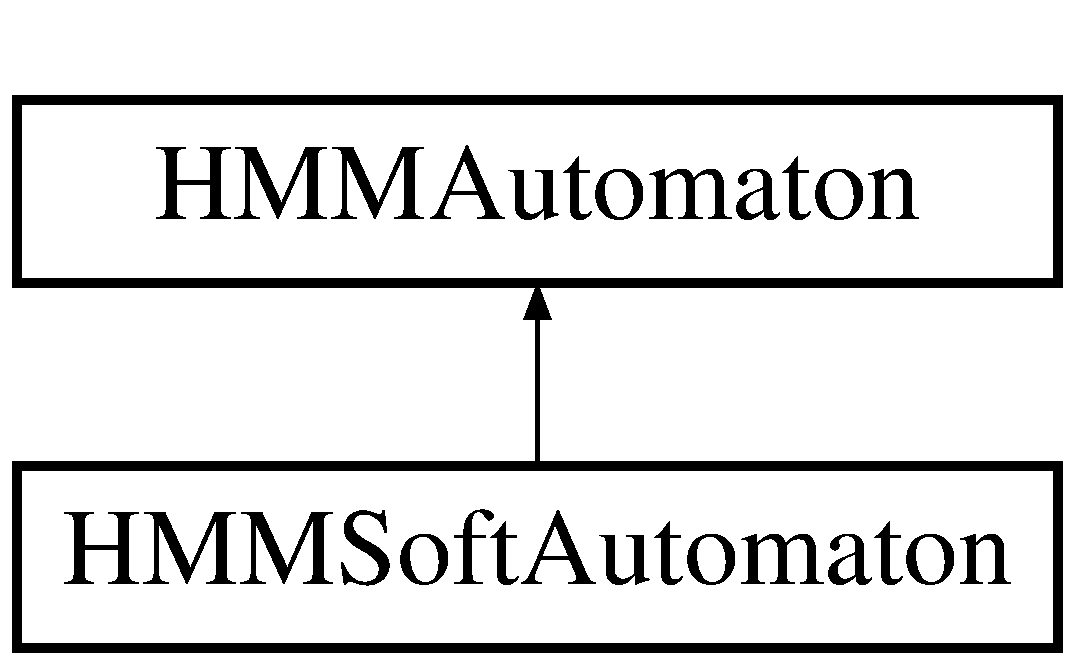
\includegraphics[height=2.000000cm]{class_h_m_m_soft_automaton}
\end{center}
\end{figure}
\subsection*{Public Member Functions}
\begin{DoxyCompactItemize}
\item 
\hyperlink{class_h_m_m_soft_automaton_aaf1234269846de3e87b3e02991768874}{H\+M\+M\+Soft\+Automaton} (std\+::vector$<$ \hyperlink{class_wave_feature_o_p}{Wave\+Feature\+O\+P} $>$ $\ast$\hyperlink{class_h_m_m_automaton_a9932eb5aa8ff484ac2406f98498595cf}{templates}, int state\+Num=\hyperlink{configure__hmm_8h_aa9cc71cb42394379957677c761aae79e}{A\+U\+T\+O\+M\+A\+T\+O\+N\+\_\+\+S\+T\+A\+T\+E\+\_\+\+N\+U\+M}, int \hyperlink{pro6__demo_8cpp_a923ffcfa3c56ccdba17bc4e700247d54}{gauss\+Num}=\hyperlink{configure__hmm_8h_a8f9db0624fff0b17f641785bb8d66a82}{G\+A\+U\+S\+S\+I\+A\+N\+\_\+\+N\+U\+M}, int train\+Times=\hyperlink{configure__hmm_8h_a52e22519b5a37e58632e9183d5197b86}{M\+A\+X\+\_\+\+T\+R\+A\+I\+N\+\_\+\+T\+I\+M\+E\+S})
\item 
\hyperlink{class_h_m_m_soft_automaton_a3a16b05052259ed3ee1fcf7e12fb343a}{$\sim$\+H\+M\+M\+Soft\+Automaton} ()
\item 
void \hyperlink{class_h_m_m_soft_automaton_ac99d24cfbfa563c54a6ee7c68b36d37e}{load} (std\+::stringstream \&in)
\item 
void \hyperlink{class_h_m_m_soft_automaton_a06c50e4f7a3461a6c6737cbe077ca0d0}{hmm\+Train} ()
\item 
double \hyperlink{class_h_m_m_soft_automaton_a4efa065f2e067d9e0b71bbf4a25bd120}{calc\+Cost} (\hyperlink{class_wave_feature_o_p}{Wave\+Feature\+O\+P} \&input)
\end{DoxyCompactItemize}
\subsection*{Private Member Functions}
\begin{DoxyCompactItemize}
\item 
\hyperlink{class_soft_state}{Soft\+State} $\ast$ \hyperlink{class_h_m_m_soft_automaton_a64b264ab97c10c015dd3951dcc0ab876}{get\+State} (int idx)
\item 
void \hyperlink{class_h_m_m_soft_automaton_a0761925dd18d2111c15e22414fa57bbb}{clear\+Train\+Buffer} ()
\item 
void \hyperlink{class_h_m_m_soft_automaton_ade39618b914aa92c7981af121a61ed5a}{before\+Alpha\+Beta} (\hyperlink{class_wave_feature_o_p}{Wave\+Feature\+O\+P} \&\hyperlink{lpc2cep_8m_afcc1d2df0288347ea10603033506e33b}{features})
\item 
void \hyperlink{class_h_m_m_soft_automaton_a9d9a82629bf46fe3bc4bd2bc58123a22}{calc\+Alpha\+Beta} (\hyperlink{class_wave_feature_o_p}{Wave\+Feature\+O\+P} \&\hyperlink{lpc2cep_8m_afcc1d2df0288347ea10603033506e33b}{features})
\item 
void \hyperlink{class_h_m_m_soft_automaton_aa5d4e88fe215f24a5eaa12c60db22793}{init\+Iterate} ()
\item 
bool \hyperlink{class_h_m_m_soft_automaton_a884b343c9fa895b4b4ef5dfe9cb7b34d}{iterate\+Train} ()
\item 
bool \hyperlink{class_h_m_m_soft_automaton_a599134520b7f52af954dddf0c431194a}{update\+Transfer} ()
\item 
void \hyperlink{class_h_m_m_soft_automaton_a158630545b1dd4bbdf1c853d44a88722}{update\+Template\+Node} (int template\+Idx)
\item 
void \hyperlink{class_h_m_m_soft_automaton_a7267e6775f4e702c94b8b89418e11504}{update\+Template\+Transfer} (int template\+Idx)
\end{DoxyCompactItemize}
\subsection*{Private Attributes}
\begin{DoxyCompactItemize}
\item 
std\+::vector$<$ double $>$ \hyperlink{class_h_m_m_soft_automaton_af71284a9b8b08b442aff84a41a89b47e}{Yust\+Cost}
\item 
\hyperlink{configure__basic_8h_a566a006016cf65b1b01bd2bc633e1c12}{Matrix}$<$ double $>$ \hyperlink{class_h_m_m_soft_automaton_ab27fbd9c234c186025e864a216fb5081}{Ys2s\+Nxt\+Cost}
\item 
\hyperlink{configure__basic_8h_a566a006016cf65b1b01bd2bc633e1c12}{Matrix}$<$ double $>$ \hyperlink{class_h_m_m_soft_automaton_ab31c1d1e1011fe8488e44fe944390a72}{node\+Cost\+Tmp}
\item 
\hyperlink{configure__basic_8h_a566a006016cf65b1b01bd2bc633e1c12}{Matrix}$<$ double $>$ \hyperlink{class_h_m_m_soft_automaton_a01e5c46f2bdfbbb6f838c1a9b7c6da21}{alpha\+Cost}
\item 
\hyperlink{configure__basic_8h_a566a006016cf65b1b01bd2bc633e1c12}{Matrix}$<$ double $>$ \hyperlink{class_h_m_m_soft_automaton_a4e2558ddec8bd8bf0eb4dd25e241d6e9}{beta\+Cost}
\end{DoxyCompactItemize}
\subsection*{Additional Inherited Members}


\subsection{Constructor \& Destructor Documentation}
\hypertarget{class_h_m_m_soft_automaton_aaf1234269846de3e87b3e02991768874}{\index{H\+M\+M\+Soft\+Automaton@{H\+M\+M\+Soft\+Automaton}!H\+M\+M\+Soft\+Automaton@{H\+M\+M\+Soft\+Automaton}}
\index{H\+M\+M\+Soft\+Automaton@{H\+M\+M\+Soft\+Automaton}!H\+M\+M\+Soft\+Automaton@{H\+M\+M\+Soft\+Automaton}}
\subsubsection[{H\+M\+M\+Soft\+Automaton}]{\setlength{\rightskip}{0pt plus 5cm}H\+M\+M\+Soft\+Automaton\+::\+H\+M\+M\+Soft\+Automaton (
\begin{DoxyParamCaption}
\item[{std\+::vector$<$ {\bf Wave\+Feature\+O\+P} $>$ $\ast$}]{templates, }
\item[{int}]{state\+Num = {\ttfamily {\bf A\+U\+T\+O\+M\+A\+T\+O\+N\+\_\+\+S\+T\+A\+T\+E\+\_\+\+N\+U\+M}}, }
\item[{int}]{gauss\+Num = {\ttfamily {\bf G\+A\+U\+S\+S\+I\+A\+N\+\_\+\+N\+U\+M}}, }
\item[{int}]{train\+Times = {\ttfamily {\bf M\+A\+X\+\_\+\+T\+R\+A\+I\+N\+\_\+\+T\+I\+M\+E\+S}}}
\end{DoxyParamCaption}
)}}\label{class_h_m_m_soft_automaton_aaf1234269846de3e87b3e02991768874}
\hypertarget{class_h_m_m_soft_automaton_a3a16b05052259ed3ee1fcf7e12fb343a}{\index{H\+M\+M\+Soft\+Automaton@{H\+M\+M\+Soft\+Automaton}!````~H\+M\+M\+Soft\+Automaton@{$\sim$\+H\+M\+M\+Soft\+Automaton}}
\index{````~H\+M\+M\+Soft\+Automaton@{$\sim$\+H\+M\+M\+Soft\+Automaton}!H\+M\+M\+Soft\+Automaton@{H\+M\+M\+Soft\+Automaton}}
\subsubsection[{$\sim$\+H\+M\+M\+Soft\+Automaton}]{\setlength{\rightskip}{0pt plus 5cm}H\+M\+M\+Soft\+Automaton\+::$\sim$\+H\+M\+M\+Soft\+Automaton (
\begin{DoxyParamCaption}
{}
\end{DoxyParamCaption}
)}}\label{class_h_m_m_soft_automaton_a3a16b05052259ed3ee1fcf7e12fb343a}


\subsection{Member Function Documentation}
\hypertarget{class_h_m_m_soft_automaton_ade39618b914aa92c7981af121a61ed5a}{\index{H\+M\+M\+Soft\+Automaton@{H\+M\+M\+Soft\+Automaton}!before\+Alpha\+Beta@{before\+Alpha\+Beta}}
\index{before\+Alpha\+Beta@{before\+Alpha\+Beta}!H\+M\+M\+Soft\+Automaton@{H\+M\+M\+Soft\+Automaton}}
\subsubsection[{before\+Alpha\+Beta}]{\setlength{\rightskip}{0pt plus 5cm}void H\+M\+M\+Soft\+Automaton\+::before\+Alpha\+Beta (
\begin{DoxyParamCaption}
\item[{{\bf Wave\+Feature\+O\+P} \&}]{features}
\end{DoxyParamCaption}
)\hspace{0.3cm}{\ttfamily [private]}}}\label{class_h_m_m_soft_automaton_ade39618b914aa92c7981af121a61ed5a}
\hypertarget{class_h_m_m_soft_automaton_a9d9a82629bf46fe3bc4bd2bc58123a22}{\index{H\+M\+M\+Soft\+Automaton@{H\+M\+M\+Soft\+Automaton}!calc\+Alpha\+Beta@{calc\+Alpha\+Beta}}
\index{calc\+Alpha\+Beta@{calc\+Alpha\+Beta}!H\+M\+M\+Soft\+Automaton@{H\+M\+M\+Soft\+Automaton}}
\subsubsection[{calc\+Alpha\+Beta}]{\setlength{\rightskip}{0pt plus 5cm}void H\+M\+M\+Soft\+Automaton\+::calc\+Alpha\+Beta (
\begin{DoxyParamCaption}
\item[{{\bf Wave\+Feature\+O\+P} \&}]{features}
\end{DoxyParamCaption}
)\hspace{0.3cm}{\ttfamily [private]}}}\label{class_h_m_m_soft_automaton_a9d9a82629bf46fe3bc4bd2bc58123a22}
\hypertarget{class_h_m_m_soft_automaton_a4efa065f2e067d9e0b71bbf4a25bd120}{\index{H\+M\+M\+Soft\+Automaton@{H\+M\+M\+Soft\+Automaton}!calc\+Cost@{calc\+Cost}}
\index{calc\+Cost@{calc\+Cost}!H\+M\+M\+Soft\+Automaton@{H\+M\+M\+Soft\+Automaton}}
\subsubsection[{calc\+Cost}]{\setlength{\rightskip}{0pt plus 5cm}double H\+M\+M\+Soft\+Automaton\+::calc\+Cost (
\begin{DoxyParamCaption}
\item[{{\bf Wave\+Feature\+O\+P} \&}]{input}
\end{DoxyParamCaption}
)\hspace{0.3cm}{\ttfamily [virtual]}}}\label{class_h_m_m_soft_automaton_a4efa065f2e067d9e0b71bbf4a25bd120}


Implements \hyperlink{class_h_m_m_automaton_a4c43e2b6bba8c6f237bf4503d79b1f12}{H\+M\+M\+Automaton}.

\hypertarget{class_h_m_m_soft_automaton_a0761925dd18d2111c15e22414fa57bbb}{\index{H\+M\+M\+Soft\+Automaton@{H\+M\+M\+Soft\+Automaton}!clear\+Train\+Buffer@{clear\+Train\+Buffer}}
\index{clear\+Train\+Buffer@{clear\+Train\+Buffer}!H\+M\+M\+Soft\+Automaton@{H\+M\+M\+Soft\+Automaton}}
\subsubsection[{clear\+Train\+Buffer}]{\setlength{\rightskip}{0pt plus 5cm}void H\+M\+M\+Soft\+Automaton\+::clear\+Train\+Buffer (
\begin{DoxyParamCaption}
{}
\end{DoxyParamCaption}
)\hspace{0.3cm}{\ttfamily [inline]}, {\ttfamily [private]}}}\label{class_h_m_m_soft_automaton_a0761925dd18d2111c15e22414fa57bbb}
\hypertarget{class_h_m_m_soft_automaton_a64b264ab97c10c015dd3951dcc0ab876}{\index{H\+M\+M\+Soft\+Automaton@{H\+M\+M\+Soft\+Automaton}!get\+State@{get\+State}}
\index{get\+State@{get\+State}!H\+M\+M\+Soft\+Automaton@{H\+M\+M\+Soft\+Automaton}}
\subsubsection[{get\+State}]{\setlength{\rightskip}{0pt plus 5cm}{\bf Soft\+State}$\ast$ H\+M\+M\+Soft\+Automaton\+::get\+State (
\begin{DoxyParamCaption}
\item[{int}]{idx}
\end{DoxyParamCaption}
)\hspace{0.3cm}{\ttfamily [inline]}, {\ttfamily [private]}}}\label{class_h_m_m_soft_automaton_a64b264ab97c10c015dd3951dcc0ab876}
\hypertarget{class_h_m_m_soft_automaton_a06c50e4f7a3461a6c6737cbe077ca0d0}{\index{H\+M\+M\+Soft\+Automaton@{H\+M\+M\+Soft\+Automaton}!hmm\+Train@{hmm\+Train}}
\index{hmm\+Train@{hmm\+Train}!H\+M\+M\+Soft\+Automaton@{H\+M\+M\+Soft\+Automaton}}
\subsubsection[{hmm\+Train}]{\setlength{\rightskip}{0pt plus 5cm}void H\+M\+M\+Soft\+Automaton\+::hmm\+Train (
\begin{DoxyParamCaption}
{}
\end{DoxyParamCaption}
)\hspace{0.3cm}{\ttfamily [virtual]}}}\label{class_h_m_m_soft_automaton_a06c50e4f7a3461a6c6737cbe077ca0d0}


Implements \hyperlink{class_h_m_m_automaton_ac6bbc2770cb11b1c9e55cd0652fbe0e3}{H\+M\+M\+Automaton}.

\hypertarget{class_h_m_m_soft_automaton_aa5d4e88fe215f24a5eaa12c60db22793}{\index{H\+M\+M\+Soft\+Automaton@{H\+M\+M\+Soft\+Automaton}!init\+Iterate@{init\+Iterate}}
\index{init\+Iterate@{init\+Iterate}!H\+M\+M\+Soft\+Automaton@{H\+M\+M\+Soft\+Automaton}}
\subsubsection[{init\+Iterate}]{\setlength{\rightskip}{0pt plus 5cm}void H\+M\+M\+Soft\+Automaton\+::init\+Iterate (
\begin{DoxyParamCaption}
{}
\end{DoxyParamCaption}
)\hspace{0.3cm}{\ttfamily [private]}}}\label{class_h_m_m_soft_automaton_aa5d4e88fe215f24a5eaa12c60db22793}
\hypertarget{class_h_m_m_soft_automaton_a884b343c9fa895b4b4ef5dfe9cb7b34d}{\index{H\+M\+M\+Soft\+Automaton@{H\+M\+M\+Soft\+Automaton}!iterate\+Train@{iterate\+Train}}
\index{iterate\+Train@{iterate\+Train}!H\+M\+M\+Soft\+Automaton@{H\+M\+M\+Soft\+Automaton}}
\subsubsection[{iterate\+Train}]{\setlength{\rightskip}{0pt plus 5cm}bool H\+M\+M\+Soft\+Automaton\+::iterate\+Train (
\begin{DoxyParamCaption}
{}
\end{DoxyParamCaption}
)\hspace{0.3cm}{\ttfamily [private]}}}\label{class_h_m_m_soft_automaton_a884b343c9fa895b4b4ef5dfe9cb7b34d}
\hypertarget{class_h_m_m_soft_automaton_ac99d24cfbfa563c54a6ee7c68b36d37e}{\index{H\+M\+M\+Soft\+Automaton@{H\+M\+M\+Soft\+Automaton}!load@{load}}
\index{load@{load}!H\+M\+M\+Soft\+Automaton@{H\+M\+M\+Soft\+Automaton}}
\subsubsection[{load}]{\setlength{\rightskip}{0pt plus 5cm}void H\+M\+M\+Soft\+Automaton\+::load (
\begin{DoxyParamCaption}
\item[{std\+::stringstream \&}]{in}
\end{DoxyParamCaption}
)\hspace{0.3cm}{\ttfamily [inline]}, {\ttfamily [virtual]}}}\label{class_h_m_m_soft_automaton_ac99d24cfbfa563c54a6ee7c68b36d37e}


Implements \hyperlink{class_h_m_m_automaton_a04b64e19e77d5fe8b78d471470346872}{H\+M\+M\+Automaton}.

\hypertarget{class_h_m_m_soft_automaton_a158630545b1dd4bbdf1c853d44a88722}{\index{H\+M\+M\+Soft\+Automaton@{H\+M\+M\+Soft\+Automaton}!update\+Template\+Node@{update\+Template\+Node}}
\index{update\+Template\+Node@{update\+Template\+Node}!H\+M\+M\+Soft\+Automaton@{H\+M\+M\+Soft\+Automaton}}
\subsubsection[{update\+Template\+Node}]{\setlength{\rightskip}{0pt plus 5cm}void H\+M\+M\+Soft\+Automaton\+::update\+Template\+Node (
\begin{DoxyParamCaption}
\item[{int}]{template\+Idx}
\end{DoxyParamCaption}
)\hspace{0.3cm}{\ttfamily [private]}}}\label{class_h_m_m_soft_automaton_a158630545b1dd4bbdf1c853d44a88722}
\hypertarget{class_h_m_m_soft_automaton_a7267e6775f4e702c94b8b89418e11504}{\index{H\+M\+M\+Soft\+Automaton@{H\+M\+M\+Soft\+Automaton}!update\+Template\+Transfer@{update\+Template\+Transfer}}
\index{update\+Template\+Transfer@{update\+Template\+Transfer}!H\+M\+M\+Soft\+Automaton@{H\+M\+M\+Soft\+Automaton}}
\subsubsection[{update\+Template\+Transfer}]{\setlength{\rightskip}{0pt plus 5cm}void H\+M\+M\+Soft\+Automaton\+::update\+Template\+Transfer (
\begin{DoxyParamCaption}
\item[{int}]{template\+Idx}
\end{DoxyParamCaption}
)\hspace{0.3cm}{\ttfamily [private]}}}\label{class_h_m_m_soft_automaton_a7267e6775f4e702c94b8b89418e11504}
\hypertarget{class_h_m_m_soft_automaton_a599134520b7f52af954dddf0c431194a}{\index{H\+M\+M\+Soft\+Automaton@{H\+M\+M\+Soft\+Automaton}!update\+Transfer@{update\+Transfer}}
\index{update\+Transfer@{update\+Transfer}!H\+M\+M\+Soft\+Automaton@{H\+M\+M\+Soft\+Automaton}}
\subsubsection[{update\+Transfer}]{\setlength{\rightskip}{0pt plus 5cm}bool H\+M\+M\+Soft\+Automaton\+::update\+Transfer (
\begin{DoxyParamCaption}
{}
\end{DoxyParamCaption}
)\hspace{0.3cm}{\ttfamily [private]}}}\label{class_h_m_m_soft_automaton_a599134520b7f52af954dddf0c431194a}


\subsection{Member Data Documentation}
\hypertarget{class_h_m_m_soft_automaton_a01e5c46f2bdfbbb6f838c1a9b7c6da21}{\index{H\+M\+M\+Soft\+Automaton@{H\+M\+M\+Soft\+Automaton}!alpha\+Cost@{alpha\+Cost}}
\index{alpha\+Cost@{alpha\+Cost}!H\+M\+M\+Soft\+Automaton@{H\+M\+M\+Soft\+Automaton}}
\subsubsection[{alpha\+Cost}]{\setlength{\rightskip}{0pt plus 5cm}{\bf Matrix}$<$double$>$ H\+M\+M\+Soft\+Automaton\+::alpha\+Cost\hspace{0.3cm}{\ttfamily [private]}}}\label{class_h_m_m_soft_automaton_a01e5c46f2bdfbbb6f838c1a9b7c6da21}
\hypertarget{class_h_m_m_soft_automaton_a4e2558ddec8bd8bf0eb4dd25e241d6e9}{\index{H\+M\+M\+Soft\+Automaton@{H\+M\+M\+Soft\+Automaton}!beta\+Cost@{beta\+Cost}}
\index{beta\+Cost@{beta\+Cost}!H\+M\+M\+Soft\+Automaton@{H\+M\+M\+Soft\+Automaton}}
\subsubsection[{beta\+Cost}]{\setlength{\rightskip}{0pt plus 5cm}{\bf Matrix}$<$double$>$ H\+M\+M\+Soft\+Automaton\+::beta\+Cost\hspace{0.3cm}{\ttfamily [private]}}}\label{class_h_m_m_soft_automaton_a4e2558ddec8bd8bf0eb4dd25e241d6e9}
\hypertarget{class_h_m_m_soft_automaton_ab31c1d1e1011fe8488e44fe944390a72}{\index{H\+M\+M\+Soft\+Automaton@{H\+M\+M\+Soft\+Automaton}!node\+Cost\+Tmp@{node\+Cost\+Tmp}}
\index{node\+Cost\+Tmp@{node\+Cost\+Tmp}!H\+M\+M\+Soft\+Automaton@{H\+M\+M\+Soft\+Automaton}}
\subsubsection[{node\+Cost\+Tmp}]{\setlength{\rightskip}{0pt plus 5cm}{\bf Matrix}$<$double$>$ H\+M\+M\+Soft\+Automaton\+::node\+Cost\+Tmp\hspace{0.3cm}{\ttfamily [private]}}}\label{class_h_m_m_soft_automaton_ab31c1d1e1011fe8488e44fe944390a72}
\hypertarget{class_h_m_m_soft_automaton_ab27fbd9c234c186025e864a216fb5081}{\index{H\+M\+M\+Soft\+Automaton@{H\+M\+M\+Soft\+Automaton}!Ys2s\+Nxt\+Cost@{Ys2s\+Nxt\+Cost}}
\index{Ys2s\+Nxt\+Cost@{Ys2s\+Nxt\+Cost}!H\+M\+M\+Soft\+Automaton@{H\+M\+M\+Soft\+Automaton}}
\subsubsection[{Ys2s\+Nxt\+Cost}]{\setlength{\rightskip}{0pt plus 5cm}{\bf Matrix}$<$double$>$ H\+M\+M\+Soft\+Automaton\+::\+Ys2s\+Nxt\+Cost\hspace{0.3cm}{\ttfamily [private]}}}\label{class_h_m_m_soft_automaton_ab27fbd9c234c186025e864a216fb5081}
\hypertarget{class_h_m_m_soft_automaton_af71284a9b8b08b442aff84a41a89b47e}{\index{H\+M\+M\+Soft\+Automaton@{H\+M\+M\+Soft\+Automaton}!Yust\+Cost@{Yust\+Cost}}
\index{Yust\+Cost@{Yust\+Cost}!H\+M\+M\+Soft\+Automaton@{H\+M\+M\+Soft\+Automaton}}
\subsubsection[{Yust\+Cost}]{\setlength{\rightskip}{0pt plus 5cm}std\+::vector$<$double$>$ H\+M\+M\+Soft\+Automaton\+::\+Yust\+Cost\hspace{0.3cm}{\ttfamily [private]}}}\label{class_h_m_m_soft_automaton_af71284a9b8b08b442aff84a41a89b47e}


The documentation for this class was generated from the following files\+:\begin{DoxyCompactItemize}
\item 
src/\+Feature/\hyperlink{_h_m_m_soft_automaton_8h}{H\+M\+M\+Soft\+Automaton.\+h}\item 
src/\+Feature/\hyperlink{_h_m_m_soft_automaton_8cpp}{H\+M\+M\+Soft\+Automaton.\+cpp}\end{DoxyCompactItemize}

\hypertarget{class_h_m_m_state}{\section{H\+M\+M\+State Class Reference}
\label{class_h_m_m_state}\index{H\+M\+M\+State@{H\+M\+M\+State}}
}


{\ttfamily \#include $<$H\+M\+M\+State.\+h$>$}

Inheritance diagram for H\+M\+M\+State\+:\begin{figure}[H]
\begin{center}
\leavevmode
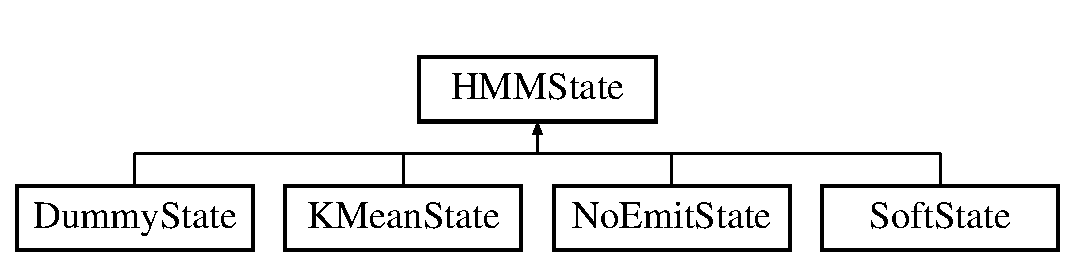
\includegraphics[height=2.000000cm]{class_h_m_m_state}
\end{center}
\end{figure}
\subsection*{Public Types}
\begin{DoxyCompactItemize}
\item 
enum \hyperlink{class_h_m_m_state_a35d2a059c2410a52110329b637940046}{State\+Type} \{ \hyperlink{class_h_m_m_state_a35d2a059c2410a52110329b637940046a44d3daf65ad0a10c73a516206a560674}{D\+U\+M\+M\+Y}, 
\hyperlink{class_h_m_m_state_a35d2a059c2410a52110329b637940046a8d417cf0b48847cc5bff7f61bf3e5d05}{K\+M\+E\+A\+N}, 
\hyperlink{class_h_m_m_state_a35d2a059c2410a52110329b637940046a2ac5e5594010c11b84fea15cc984b3aa}{S\+O\+F\+T}, 
\hyperlink{class_h_m_m_state_a35d2a059c2410a52110329b637940046aa8661e1ac291d403c548214337b3bcab}{U\+N\+E\+M\+I\+T}
 \}
\end{DoxyCompactItemize}
\subsection*{Public Member Functions}
\begin{DoxyCompactItemize}
\item 
\hyperlink{class_h_m_m_state_a5ba34d8b1512868d649194ba16442d5b}{H\+M\+M\+State} (std\+::vector$<$ \hyperlink{class_wave_feature_o_p}{Wave\+Feature\+O\+P} $>$ $\ast$\hyperlink{class_h_m_m_state_a04d0b1a1570a339e5cd0db13aeb0d2ae}{templates})
\item 
\hyperlink{class_h_m_m_state_a7fc28ceacfa7f99b36f19523db1da73f}{H\+M\+M\+State} ()
\item 
virtual \hyperlink{class_h_m_m_state_ab2bdc4eb99ff598d7b1b2185bdaa457d}{$\sim$\+H\+M\+M\+State} ()
\item 
virtual void \hyperlink{class_h_m_m_state_a2d42dd972a85014c0f5f9875da1eacd7}{gaussian\+Train} (int gaussian\+Num)=0
\item 
virtual double \hyperlink{class_h_m_m_state_a84ad1899239f79257837e6d77cc4f242}{node\+Cost} (\hyperlink{class_feature}{Feature} $\ast$input\+Feature)=0
\item 
virtual void \hyperlink{class_h_m_m_state_ab9d6387b87e62ac03f4d15db1da7d7c7}{set\+Templates} (std\+::vector$<$ \hyperlink{class_wave_feature_o_p}{Wave\+Feature\+O\+P} $>$ $\ast$new\+Temps)
\item 
virtual void \hyperlink{class_h_m_m_state_ad5d14bf058b8fc39e07319fabebe09ee}{load} (std\+::stringstream \&in, int \&\hyperlink{pro6__demo_8cpp_a923ffcfa3c56ccdba17bc4e700247d54}{gauss\+Num})=0
\item 
virtual void \hyperlink{class_h_m_m_state_ab12116fc28ade677ee79ff13b4577ea6}{store} (std\+::stringstream \&out)=0
\end{DoxyCompactItemize}
\subsection*{Protected Attributes}
\begin{DoxyCompactItemize}
\item 
std\+::vector$<$ \hyperlink{class_wave_feature_o_p}{Wave\+Feature\+O\+P} $>$ $\ast$ \hyperlink{class_h_m_m_state_a04d0b1a1570a339e5cd0db13aeb0d2ae}{templates}
\end{DoxyCompactItemize}
\subsection*{Friends}
\begin{DoxyCompactItemize}
\item 
class \hyperlink{class_h_m_m_state_a3f73063e67c75773ba856636249277b6}{H\+M\+M\+Automaton}
\end{DoxyCompactItemize}


\subsection{Member Enumeration Documentation}
\hypertarget{class_h_m_m_state_a35d2a059c2410a52110329b637940046}{\index{H\+M\+M\+State@{H\+M\+M\+State}!State\+Type@{State\+Type}}
\index{State\+Type@{State\+Type}!H\+M\+M\+State@{H\+M\+M\+State}}
\subsubsection[{State\+Type}]{\setlength{\rightskip}{0pt plus 5cm}enum {\bf H\+M\+M\+State\+::\+State\+Type}}}\label{class_h_m_m_state_a35d2a059c2410a52110329b637940046}
\begin{Desc}
\item[Enumerator]\par
\begin{description}
\index{D\+U\+M\+M\+Y@{D\+U\+M\+M\+Y}!H\+M\+M\+State@{H\+M\+M\+State}}\index{H\+M\+M\+State@{H\+M\+M\+State}!D\+U\+M\+M\+Y@{D\+U\+M\+M\+Y}}\item[{\em 
\hypertarget{class_h_m_m_state_a35d2a059c2410a52110329b637940046a44d3daf65ad0a10c73a516206a560674}{D\+U\+M\+M\+Y}\label{class_h_m_m_state_a35d2a059c2410a52110329b637940046a44d3daf65ad0a10c73a516206a560674}
}]\index{K\+M\+E\+A\+N@{K\+M\+E\+A\+N}!H\+M\+M\+State@{H\+M\+M\+State}}\index{H\+M\+M\+State@{H\+M\+M\+State}!K\+M\+E\+A\+N@{K\+M\+E\+A\+N}}\item[{\em 
\hypertarget{class_h_m_m_state_a35d2a059c2410a52110329b637940046a8d417cf0b48847cc5bff7f61bf3e5d05}{K\+M\+E\+A\+N}\label{class_h_m_m_state_a35d2a059c2410a52110329b637940046a8d417cf0b48847cc5bff7f61bf3e5d05}
}]\index{S\+O\+F\+T@{S\+O\+F\+T}!H\+M\+M\+State@{H\+M\+M\+State}}\index{H\+M\+M\+State@{H\+M\+M\+State}!S\+O\+F\+T@{S\+O\+F\+T}}\item[{\em 
\hypertarget{class_h_m_m_state_a35d2a059c2410a52110329b637940046a2ac5e5594010c11b84fea15cc984b3aa}{S\+O\+F\+T}\label{class_h_m_m_state_a35d2a059c2410a52110329b637940046a2ac5e5594010c11b84fea15cc984b3aa}
}]\index{U\+N\+E\+M\+I\+T@{U\+N\+E\+M\+I\+T}!H\+M\+M\+State@{H\+M\+M\+State}}\index{H\+M\+M\+State@{H\+M\+M\+State}!U\+N\+E\+M\+I\+T@{U\+N\+E\+M\+I\+T}}\item[{\em 
\hypertarget{class_h_m_m_state_a35d2a059c2410a52110329b637940046aa8661e1ac291d403c548214337b3bcab}{U\+N\+E\+M\+I\+T}\label{class_h_m_m_state_a35d2a059c2410a52110329b637940046aa8661e1ac291d403c548214337b3bcab}
}]\end{description}
\end{Desc}


\subsection{Constructor \& Destructor Documentation}
\hypertarget{class_h_m_m_state_a5ba34d8b1512868d649194ba16442d5b}{\index{H\+M\+M\+State@{H\+M\+M\+State}!H\+M\+M\+State@{H\+M\+M\+State}}
\index{H\+M\+M\+State@{H\+M\+M\+State}!H\+M\+M\+State@{H\+M\+M\+State}}
\subsubsection[{H\+M\+M\+State}]{\setlength{\rightskip}{0pt plus 5cm}H\+M\+M\+State\+::\+H\+M\+M\+State (
\begin{DoxyParamCaption}
\item[{std\+::vector$<$ {\bf Wave\+Feature\+O\+P} $>$ $\ast$}]{templates}
\end{DoxyParamCaption}
)\hspace{0.3cm}{\ttfamily [inline]}}}\label{class_h_m_m_state_a5ba34d8b1512868d649194ba16442d5b}
\hypertarget{class_h_m_m_state_a7fc28ceacfa7f99b36f19523db1da73f}{\index{H\+M\+M\+State@{H\+M\+M\+State}!H\+M\+M\+State@{H\+M\+M\+State}}
\index{H\+M\+M\+State@{H\+M\+M\+State}!H\+M\+M\+State@{H\+M\+M\+State}}
\subsubsection[{H\+M\+M\+State}]{\setlength{\rightskip}{0pt plus 5cm}H\+M\+M\+State\+::\+H\+M\+M\+State (
\begin{DoxyParamCaption}
{}
\end{DoxyParamCaption}
)\hspace{0.3cm}{\ttfamily [inline]}}}\label{class_h_m_m_state_a7fc28ceacfa7f99b36f19523db1da73f}
\hypertarget{class_h_m_m_state_ab2bdc4eb99ff598d7b1b2185bdaa457d}{\index{H\+M\+M\+State@{H\+M\+M\+State}!````~H\+M\+M\+State@{$\sim$\+H\+M\+M\+State}}
\index{````~H\+M\+M\+State@{$\sim$\+H\+M\+M\+State}!H\+M\+M\+State@{H\+M\+M\+State}}
\subsubsection[{$\sim$\+H\+M\+M\+State}]{\setlength{\rightskip}{0pt plus 5cm}virtual H\+M\+M\+State\+::$\sim$\+H\+M\+M\+State (
\begin{DoxyParamCaption}
{}
\end{DoxyParamCaption}
)\hspace{0.3cm}{\ttfamily [inline]}, {\ttfamily [virtual]}}}\label{class_h_m_m_state_ab2bdc4eb99ff598d7b1b2185bdaa457d}


\subsection{Member Function Documentation}
\hypertarget{class_h_m_m_state_a2d42dd972a85014c0f5f9875da1eacd7}{\index{H\+M\+M\+State@{H\+M\+M\+State}!gaussian\+Train@{gaussian\+Train}}
\index{gaussian\+Train@{gaussian\+Train}!H\+M\+M\+State@{H\+M\+M\+State}}
\subsubsection[{gaussian\+Train}]{\setlength{\rightskip}{0pt plus 5cm}virtual void H\+M\+M\+State\+::gaussian\+Train (
\begin{DoxyParamCaption}
\item[{int}]{gaussian\+Num}
\end{DoxyParamCaption}
)\hspace{0.3cm}{\ttfamily [pure virtual]}}}\label{class_h_m_m_state_a2d42dd972a85014c0f5f9875da1eacd7}


Implemented in \hyperlink{class_k_mean_state_a5a6269056f80bfbce8d1598c729877fa}{K\+Mean\+State}, \hyperlink{class_soft_state_ab7658b800fe20e84f8ed898d12c082a4}{Soft\+State}, \hyperlink{class_dummy_state_a3ea8e5a558e56079610eb1b0faee2ef9}{Dummy\+State}, and \hyperlink{class_no_emit_state_acb0904c7b81e54bbfa8a995e1acd47bd}{No\+Emit\+State}.

\hypertarget{class_h_m_m_state_ad5d14bf058b8fc39e07319fabebe09ee}{\index{H\+M\+M\+State@{H\+M\+M\+State}!load@{load}}
\index{load@{load}!H\+M\+M\+State@{H\+M\+M\+State}}
\subsubsection[{load}]{\setlength{\rightskip}{0pt plus 5cm}virtual void H\+M\+M\+State\+::load (
\begin{DoxyParamCaption}
\item[{std\+::stringstream \&}]{in, }
\item[{int \&}]{gauss\+Num}
\end{DoxyParamCaption}
)\hspace{0.3cm}{\ttfamily [pure virtual]}}}\label{class_h_m_m_state_ad5d14bf058b8fc39e07319fabebe09ee}


Implemented in \hyperlink{class_k_mean_state_aa84a9c40d629924d92a6816f45623f36}{K\+Mean\+State}, \hyperlink{class_soft_state_a157535fbd2cc224f30c06ac385a4377b}{Soft\+State}, \hyperlink{class_dummy_state_a7aecab0455227d309908efd3c0cdbaa3}{Dummy\+State}, and \hyperlink{class_no_emit_state_a59702d5b1bb81733c2694fe1fa80a8e6}{No\+Emit\+State}.

\hypertarget{class_h_m_m_state_a84ad1899239f79257837e6d77cc4f242}{\index{H\+M\+M\+State@{H\+M\+M\+State}!node\+Cost@{node\+Cost}}
\index{node\+Cost@{node\+Cost}!H\+M\+M\+State@{H\+M\+M\+State}}
\subsubsection[{node\+Cost}]{\setlength{\rightskip}{0pt plus 5cm}virtual double H\+M\+M\+State\+::node\+Cost (
\begin{DoxyParamCaption}
\item[{{\bf Feature} $\ast$}]{input\+Feature}
\end{DoxyParamCaption}
)\hspace{0.3cm}{\ttfamily [pure virtual]}}}\label{class_h_m_m_state_a84ad1899239f79257837e6d77cc4f242}


Implemented in \hyperlink{class_k_mean_state_a6f628235aea39397ff91d0b6509ef927}{K\+Mean\+State}, \hyperlink{class_soft_state_aefe179676d2eb32304ddd04da60208f4}{Soft\+State}, \hyperlink{class_dummy_state_a696495e250c01d42c48c6a5f79b1f1d8}{Dummy\+State}, and \hyperlink{class_no_emit_state_a37853ca0ea0cffe47d4bacf6c9f4ea3d}{No\+Emit\+State}.

\hypertarget{class_h_m_m_state_ab9d6387b87e62ac03f4d15db1da7d7c7}{\index{H\+M\+M\+State@{H\+M\+M\+State}!set\+Templates@{set\+Templates}}
\index{set\+Templates@{set\+Templates}!H\+M\+M\+State@{H\+M\+M\+State}}
\subsubsection[{set\+Templates}]{\setlength{\rightskip}{0pt plus 5cm}virtual void H\+M\+M\+State\+::set\+Templates (
\begin{DoxyParamCaption}
\item[{std\+::vector$<$ {\bf Wave\+Feature\+O\+P} $>$ $\ast$}]{new\+Temps}
\end{DoxyParamCaption}
)\hspace{0.3cm}{\ttfamily [inline]}, {\ttfamily [virtual]}}}\label{class_h_m_m_state_ab9d6387b87e62ac03f4d15db1da7d7c7}


Reimplemented in \hyperlink{class_k_mean_state_ac3a33185bbab17390b55a85ec6e270e5}{K\+Mean\+State}, and \hyperlink{class_soft_state_a5577579995771ff34512c576ddfd5885}{Soft\+State}.

\hypertarget{class_h_m_m_state_ab12116fc28ade677ee79ff13b4577ea6}{\index{H\+M\+M\+State@{H\+M\+M\+State}!store@{store}}
\index{store@{store}!H\+M\+M\+State@{H\+M\+M\+State}}
\subsubsection[{store}]{\setlength{\rightskip}{0pt plus 5cm}virtual void H\+M\+M\+State\+::store (
\begin{DoxyParamCaption}
\item[{std\+::stringstream \&}]{out}
\end{DoxyParamCaption}
)\hspace{0.3cm}{\ttfamily [pure virtual]}}}\label{class_h_m_m_state_ab12116fc28ade677ee79ff13b4577ea6}


Implemented in \hyperlink{class_k_mean_state_afaa85c369000eca4930c478809bbc54b}{K\+Mean\+State}, \hyperlink{class_soft_state_a0d8a511a0ba9a18b797ecb07f96f944f}{Soft\+State}, \hyperlink{class_dummy_state_a3759cade768196f1f920aa683336ed55}{Dummy\+State}, and \hyperlink{class_no_emit_state_afbe040ba5781ef6cf4f2544cb3756962}{No\+Emit\+State}.



\subsection{Friends And Related Function Documentation}
\hypertarget{class_h_m_m_state_a3f73063e67c75773ba856636249277b6}{\index{H\+M\+M\+State@{H\+M\+M\+State}!H\+M\+M\+Automaton@{H\+M\+M\+Automaton}}
\index{H\+M\+M\+Automaton@{H\+M\+M\+Automaton}!H\+M\+M\+State@{H\+M\+M\+State}}
\subsubsection[{H\+M\+M\+Automaton}]{\setlength{\rightskip}{0pt plus 5cm}friend class {\bf H\+M\+M\+Automaton}\hspace{0.3cm}{\ttfamily [friend]}}}\label{class_h_m_m_state_a3f73063e67c75773ba856636249277b6}


\subsection{Member Data Documentation}
\hypertarget{class_h_m_m_state_a04d0b1a1570a339e5cd0db13aeb0d2ae}{\index{H\+M\+M\+State@{H\+M\+M\+State}!templates@{templates}}
\index{templates@{templates}!H\+M\+M\+State@{H\+M\+M\+State}}
\subsubsection[{templates}]{\setlength{\rightskip}{0pt plus 5cm}std\+::vector$<${\bf Wave\+Feature\+O\+P}$>$$\ast$ H\+M\+M\+State\+::templates\hspace{0.3cm}{\ttfamily [protected]}}}\label{class_h_m_m_state_a04d0b1a1570a339e5cd0db13aeb0d2ae}


The documentation for this class was generated from the following file\+:\begin{DoxyCompactItemize}
\item 
src/\+Feature/\hyperlink{_h_m_m_state_8h}{H\+M\+M\+State.\+h}\end{DoxyCompactItemize}

\hypertarget{class_wave_feature_o_p_set_1_1iterator}{\section{Wave\+Feature\+O\+P\+Set\+:\+:iterator Class Reference}
\label{class_wave_feature_o_p_set_1_1iterator}\index{Wave\+Feature\+O\+P\+Set\+::iterator@{Wave\+Feature\+O\+P\+Set\+::iterator}}
}


{\ttfamily \#include $<$Wave\+Feature\+O\+P\+Set.\+h$>$}

\subsection*{Public Member Functions}
\begin{DoxyCompactItemize}
\item 
\hyperlink{class_wave_feature_o_p_set_1_1iterator_a106ac8443c927a9c40520b478a80372c}{iterator} (int \hyperlink{pro4__demo__1_8cpp_adc01d2f6980a1af5c3ddc83d847dafa0}{max\+Instance\+Per}=\hyperlink{configure__dtw_8h_a5e1cc8ac4ebc0912817c618ccc9d823b}{M\+A\+X\+\_\+\+T\+E\+M\+P\+L\+A\+T\+E\+S\+\_\+\+P\+E\+R\+\_\+\+W\+O\+R\+D})
\item 
\hyperlink{class_wave_feature_o_p_set_1_1iterator_ad346abddf10824562ddc0a8ac7676e39}{iterator} (\hyperlink{class_wave_feature_o_p_set_a7145e9463a1fb85ce4c239552bf4e8e0}{data\+Set\+Type} $\ast$data\+Set\+Ptr, data\+Set\+Type\+::iterator Itr, int idx, int \hyperlink{pro4__demo__1_8cpp_adc01d2f6980a1af5c3ddc83d847dafa0}{max\+Instance\+Per}=\hyperlink{configure__dtw_8h_a5e1cc8ac4ebc0912817c618ccc9d823b}{M\+A\+X\+\_\+\+T\+E\+M\+P\+L\+A\+T\+E\+S\+\_\+\+P\+E\+R\+\_\+\+W\+O\+R\+D})
\item 
\hyperlink{class_wave_feature_o_p}{Wave\+Feature\+O\+P} $\ast$ \hyperlink{class_wave_feature_o_p_set_1_1iterator_a5b55475159717135436bfaaac5fc5702}{operator$\ast$} ()
\item 
const \hyperlink{class_wave_feature_o_p_set_1_1iterator}{iterator} \& \hyperlink{class_wave_feature_o_p_set_1_1iterator_a9e47a4d0cf363ecce99432cc19f6c122}{operator++} (int)
\item 
const \hyperlink{class_wave_feature_o_p_set_1_1iterator}{iterator} \& \hyperlink{class_wave_feature_o_p_set_1_1iterator_ae32d8b6a50360369b67f22c938987a6c}{operator++} ()
\item 
const \hyperlink{class_wave_feature_o_p_set_1_1iterator}{iterator} \& \hyperlink{class_wave_feature_o_p_set_1_1iterator_a8958a82c281d0726ae26dec7f2ea6921}{next\+Word} ()
\item 
bool \hyperlink{class_wave_feature_o_p_set_1_1iterator_a429c2e56247bab88043c1de2dbb6551a}{operator==} (const \hyperlink{class_wave_feature_o_p_set_1_1iterator}{iterator} \&b)
\item 
bool \hyperlink{class_wave_feature_o_p_set_1_1iterator_a2d4e4835b6a46853d726a19dd3aab209}{operator!=} (const \hyperlink{class_wave_feature_o_p_set_1_1iterator}{iterator} \&b)
\end{DoxyCompactItemize}
\subsection*{Private Attributes}
\begin{DoxyCompactItemize}
\item 
int \hyperlink{class_wave_feature_o_p_set_1_1iterator_a94f22cdd6fcee7a6125b8b09f0384cb2}{max\+Templates\+Per\+Word}
\item 
\hyperlink{class_wave_feature_o_p_set_a7145e9463a1fb85ce4c239552bf4e8e0}{data\+Set\+Type} $\ast$ \hyperlink{class_wave_feature_o_p_set_1_1iterator_a3eb82b0712290fe15e135390a02150fa}{data\+Set}
\item 
data\+Set\+Type\+::iterator \hyperlink{class_wave_feature_o_p_set_1_1iterator_a20f89afc2f06d44b8aae87e33cc28ef6}{I}
\item 
int \hyperlink{class_wave_feature_o_p_set_1_1iterator_abf861ecdfdfb9474c1a55514d4854597}{vec\+Idx}
\end{DoxyCompactItemize}


\subsection{Constructor \& Destructor Documentation}
\hypertarget{class_wave_feature_o_p_set_1_1iterator_a106ac8443c927a9c40520b478a80372c}{\index{Wave\+Feature\+O\+P\+Set\+::iterator@{Wave\+Feature\+O\+P\+Set\+::iterator}!iterator@{iterator}}
\index{iterator@{iterator}!Wave\+Feature\+O\+P\+Set\+::iterator@{Wave\+Feature\+O\+P\+Set\+::iterator}}
\subsubsection[{iterator}]{\setlength{\rightskip}{0pt plus 5cm}Wave\+Feature\+O\+P\+Set\+::iterator\+::iterator (
\begin{DoxyParamCaption}
\item[{int}]{max\+Instance\+Per = {\ttfamily {\bf M\+A\+X\+\_\+\+T\+E\+M\+P\+L\+A\+T\+E\+S\+\_\+\+P\+E\+R\+\_\+\+W\+O\+R\+D}}}
\end{DoxyParamCaption}
)\hspace{0.3cm}{\ttfamily [inline]}}}\label{class_wave_feature_o_p_set_1_1iterator_a106ac8443c927a9c40520b478a80372c}
\hypertarget{class_wave_feature_o_p_set_1_1iterator_ad346abddf10824562ddc0a8ac7676e39}{\index{Wave\+Feature\+O\+P\+Set\+::iterator@{Wave\+Feature\+O\+P\+Set\+::iterator}!iterator@{iterator}}
\index{iterator@{iterator}!Wave\+Feature\+O\+P\+Set\+::iterator@{Wave\+Feature\+O\+P\+Set\+::iterator}}
\subsubsection[{iterator}]{\setlength{\rightskip}{0pt plus 5cm}Wave\+Feature\+O\+P\+Set\+::iterator\+::iterator (
\begin{DoxyParamCaption}
\item[{{\bf data\+Set\+Type} $\ast$}]{data\+Set\+Ptr, }
\item[{data\+Set\+Type\+::iterator}]{Itr, }
\item[{int}]{idx, }
\item[{int}]{max\+Instance\+Per = {\ttfamily {\bf M\+A\+X\+\_\+\+T\+E\+M\+P\+L\+A\+T\+E\+S\+\_\+\+P\+E\+R\+\_\+\+W\+O\+R\+D}}}
\end{DoxyParamCaption}
)\hspace{0.3cm}{\ttfamily [inline]}}}\label{class_wave_feature_o_p_set_1_1iterator_ad346abddf10824562ddc0a8ac7676e39}


\subsection{Member Function Documentation}
\hypertarget{class_wave_feature_o_p_set_1_1iterator_a8958a82c281d0726ae26dec7f2ea6921}{\index{Wave\+Feature\+O\+P\+Set\+::iterator@{Wave\+Feature\+O\+P\+Set\+::iterator}!next\+Word@{next\+Word}}
\index{next\+Word@{next\+Word}!Wave\+Feature\+O\+P\+Set\+::iterator@{Wave\+Feature\+O\+P\+Set\+::iterator}}
\subsubsection[{next\+Word}]{\setlength{\rightskip}{0pt plus 5cm}const {\bf iterator}\& Wave\+Feature\+O\+P\+Set\+::iterator\+::next\+Word (
\begin{DoxyParamCaption}
{}
\end{DoxyParamCaption}
)\hspace{0.3cm}{\ttfamily [inline]}}}\label{class_wave_feature_o_p_set_1_1iterator_a8958a82c281d0726ae26dec7f2ea6921}
\hypertarget{class_wave_feature_o_p_set_1_1iterator_a2d4e4835b6a46853d726a19dd3aab209}{\index{Wave\+Feature\+O\+P\+Set\+::iterator@{Wave\+Feature\+O\+P\+Set\+::iterator}!operator"!=@{operator"!=}}
\index{operator"!=@{operator"!=}!Wave\+Feature\+O\+P\+Set\+::iterator@{Wave\+Feature\+O\+P\+Set\+::iterator}}
\subsubsection[{operator"!=}]{\setlength{\rightskip}{0pt plus 5cm}bool Wave\+Feature\+O\+P\+Set\+::iterator\+::operator!= (
\begin{DoxyParamCaption}
\item[{const {\bf iterator} \&}]{b}
\end{DoxyParamCaption}
)\hspace{0.3cm}{\ttfamily [inline]}}}\label{class_wave_feature_o_p_set_1_1iterator_a2d4e4835b6a46853d726a19dd3aab209}
\hypertarget{class_wave_feature_o_p_set_1_1iterator_a5b55475159717135436bfaaac5fc5702}{\index{Wave\+Feature\+O\+P\+Set\+::iterator@{Wave\+Feature\+O\+P\+Set\+::iterator}!operator$\ast$@{operator$\ast$}}
\index{operator$\ast$@{operator$\ast$}!Wave\+Feature\+O\+P\+Set\+::iterator@{Wave\+Feature\+O\+P\+Set\+::iterator}}
\subsubsection[{operator$\ast$}]{\setlength{\rightskip}{0pt plus 5cm}{\bf Wave\+Feature\+O\+P}$\ast$ Wave\+Feature\+O\+P\+Set\+::iterator\+::operator$\ast$ (
\begin{DoxyParamCaption}
{}
\end{DoxyParamCaption}
)\hspace{0.3cm}{\ttfamily [inline]}}}\label{class_wave_feature_o_p_set_1_1iterator_a5b55475159717135436bfaaac5fc5702}
\hypertarget{class_wave_feature_o_p_set_1_1iterator_a9e47a4d0cf363ecce99432cc19f6c122}{\index{Wave\+Feature\+O\+P\+Set\+::iterator@{Wave\+Feature\+O\+P\+Set\+::iterator}!operator++@{operator++}}
\index{operator++@{operator++}!Wave\+Feature\+O\+P\+Set\+::iterator@{Wave\+Feature\+O\+P\+Set\+::iterator}}
\subsubsection[{operator++}]{\setlength{\rightskip}{0pt plus 5cm}const {\bf iterator}\& Wave\+Feature\+O\+P\+Set\+::iterator\+::operator++ (
\begin{DoxyParamCaption}
\item[{int}]{}
\end{DoxyParamCaption}
)\hspace{0.3cm}{\ttfamily [inline]}}}\label{class_wave_feature_o_p_set_1_1iterator_a9e47a4d0cf363ecce99432cc19f6c122}
\hypertarget{class_wave_feature_o_p_set_1_1iterator_ae32d8b6a50360369b67f22c938987a6c}{\index{Wave\+Feature\+O\+P\+Set\+::iterator@{Wave\+Feature\+O\+P\+Set\+::iterator}!operator++@{operator++}}
\index{operator++@{operator++}!Wave\+Feature\+O\+P\+Set\+::iterator@{Wave\+Feature\+O\+P\+Set\+::iterator}}
\subsubsection[{operator++}]{\setlength{\rightskip}{0pt plus 5cm}const {\bf iterator}\& Wave\+Feature\+O\+P\+Set\+::iterator\+::operator++ (
\begin{DoxyParamCaption}
{}
\end{DoxyParamCaption}
)\hspace{0.3cm}{\ttfamily [inline]}}}\label{class_wave_feature_o_p_set_1_1iterator_ae32d8b6a50360369b67f22c938987a6c}
\hypertarget{class_wave_feature_o_p_set_1_1iterator_a429c2e56247bab88043c1de2dbb6551a}{\index{Wave\+Feature\+O\+P\+Set\+::iterator@{Wave\+Feature\+O\+P\+Set\+::iterator}!operator==@{operator==}}
\index{operator==@{operator==}!Wave\+Feature\+O\+P\+Set\+::iterator@{Wave\+Feature\+O\+P\+Set\+::iterator}}
\subsubsection[{operator==}]{\setlength{\rightskip}{0pt plus 5cm}bool Wave\+Feature\+O\+P\+Set\+::iterator\+::operator== (
\begin{DoxyParamCaption}
\item[{const {\bf iterator} \&}]{b}
\end{DoxyParamCaption}
)\hspace{0.3cm}{\ttfamily [inline]}}}\label{class_wave_feature_o_p_set_1_1iterator_a429c2e56247bab88043c1de2dbb6551a}


\subsection{Member Data Documentation}
\hypertarget{class_wave_feature_o_p_set_1_1iterator_a3eb82b0712290fe15e135390a02150fa}{\index{Wave\+Feature\+O\+P\+Set\+::iterator@{Wave\+Feature\+O\+P\+Set\+::iterator}!data\+Set@{data\+Set}}
\index{data\+Set@{data\+Set}!Wave\+Feature\+O\+P\+Set\+::iterator@{Wave\+Feature\+O\+P\+Set\+::iterator}}
\subsubsection[{data\+Set}]{\setlength{\rightskip}{0pt plus 5cm}{\bf data\+Set\+Type}$\ast$ Wave\+Feature\+O\+P\+Set\+::iterator\+::data\+Set\hspace{0.3cm}{\ttfamily [private]}}}\label{class_wave_feature_o_p_set_1_1iterator_a3eb82b0712290fe15e135390a02150fa}
\hypertarget{class_wave_feature_o_p_set_1_1iterator_a20f89afc2f06d44b8aae87e33cc28ef6}{\index{Wave\+Feature\+O\+P\+Set\+::iterator@{Wave\+Feature\+O\+P\+Set\+::iterator}!I@{I}}
\index{I@{I}!Wave\+Feature\+O\+P\+Set\+::iterator@{Wave\+Feature\+O\+P\+Set\+::iterator}}
\subsubsection[{I}]{\setlength{\rightskip}{0pt plus 5cm}data\+Set\+Type\+::iterator Wave\+Feature\+O\+P\+Set\+::iterator\+::\+I\hspace{0.3cm}{\ttfamily [private]}}}\label{class_wave_feature_o_p_set_1_1iterator_a20f89afc2f06d44b8aae87e33cc28ef6}
\hypertarget{class_wave_feature_o_p_set_1_1iterator_a94f22cdd6fcee7a6125b8b09f0384cb2}{\index{Wave\+Feature\+O\+P\+Set\+::iterator@{Wave\+Feature\+O\+P\+Set\+::iterator}!max\+Templates\+Per\+Word@{max\+Templates\+Per\+Word}}
\index{max\+Templates\+Per\+Word@{max\+Templates\+Per\+Word}!Wave\+Feature\+O\+P\+Set\+::iterator@{Wave\+Feature\+O\+P\+Set\+::iterator}}
\subsubsection[{max\+Templates\+Per\+Word}]{\setlength{\rightskip}{0pt plus 5cm}int Wave\+Feature\+O\+P\+Set\+::iterator\+::max\+Templates\+Per\+Word\hspace{0.3cm}{\ttfamily [private]}}}\label{class_wave_feature_o_p_set_1_1iterator_a94f22cdd6fcee7a6125b8b09f0384cb2}
\hypertarget{class_wave_feature_o_p_set_1_1iterator_abf861ecdfdfb9474c1a55514d4854597}{\index{Wave\+Feature\+O\+P\+Set\+::iterator@{Wave\+Feature\+O\+P\+Set\+::iterator}!vec\+Idx@{vec\+Idx}}
\index{vec\+Idx@{vec\+Idx}!Wave\+Feature\+O\+P\+Set\+::iterator@{Wave\+Feature\+O\+P\+Set\+::iterator}}
\subsubsection[{vec\+Idx}]{\setlength{\rightskip}{0pt plus 5cm}int Wave\+Feature\+O\+P\+Set\+::iterator\+::vec\+Idx\hspace{0.3cm}{\ttfamily [private]}}}\label{class_wave_feature_o_p_set_1_1iterator_abf861ecdfdfb9474c1a55514d4854597}


The documentation for this class was generated from the following file\+:\begin{DoxyCompactItemize}
\item 
src/\+Feature/\hyperlink{_wave_feature_o_p_set_8h}{Wave\+Feature\+O\+P\+Set.\+h}\end{DoxyCompactItemize}

\hypertarget{class_k_mean_state}{\section{K\+Mean\+State Class Reference}
\label{class_k_mean_state}\index{K\+Mean\+State@{K\+Mean\+State}}
}


{\ttfamily \#include $<$K\+Mean\+State.\+h$>$}

Inheritance diagram for K\+Mean\+State\+:\begin{figure}[H]
\begin{center}
\leavevmode
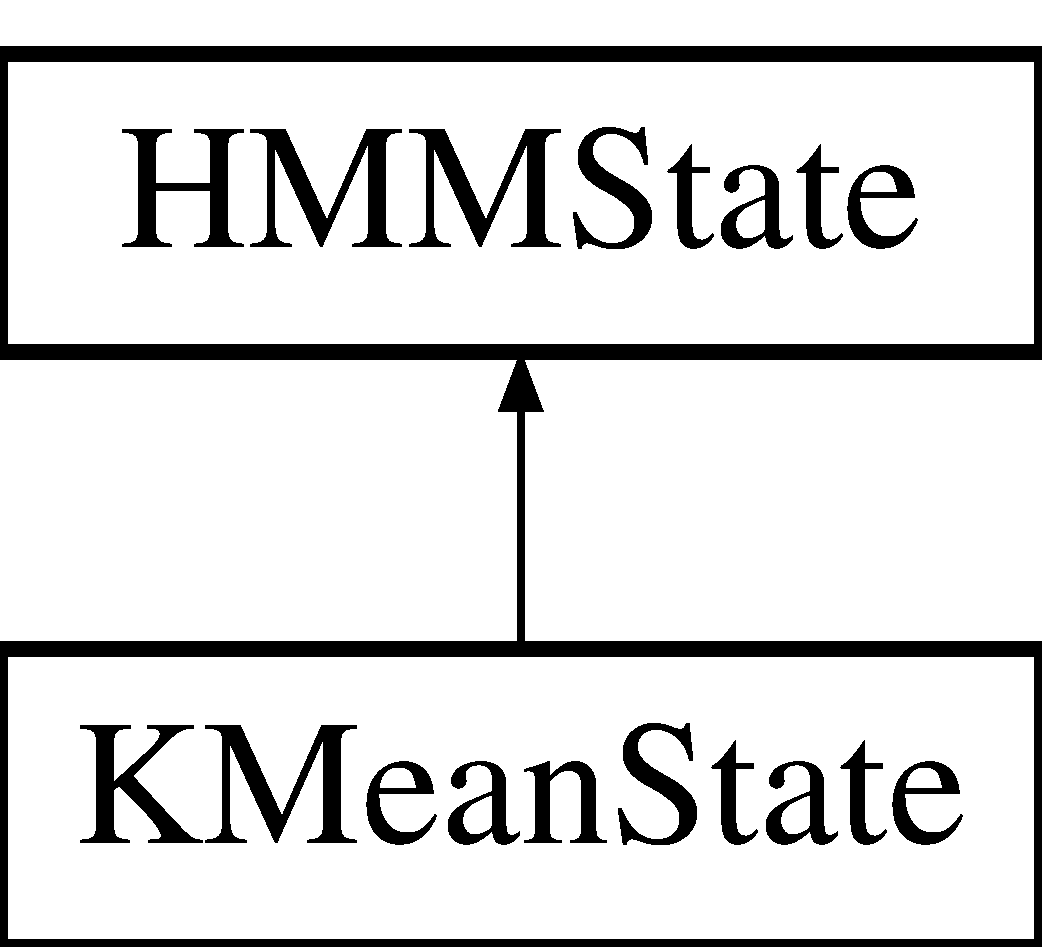
\includegraphics[height=2.000000cm]{class_k_mean_state}
\end{center}
\end{figure}
\subsection*{Public Member Functions}
\begin{DoxyCompactItemize}
\item 
\hyperlink{class_k_mean_state_a514a6b2326e2236e63edf3087a6e21dd}{K\+Mean\+State} (std\+::vector$<$ \hyperlink{class_wave_feature_o_p}{Wave\+Feature\+O\+P} $>$ $\ast$\hyperlink{class_h_m_m_state_a04d0b1a1570a339e5cd0db13aeb0d2ae}{templates})
\item 
\hyperlink{class_k_mean_state_a0889842e49b26726cb31942de9751de2}{$\sim$\+K\+Mean\+State} ()
\item 
void \hyperlink{class_k_mean_state_a5a6269056f80bfbce8d1598c729877fa}{gaussian\+Train} (int gaussian\+Num)
\item 
double \hyperlink{class_k_mean_state_a6f628235aea39397ff91d0b6509ef927}{node\+Cost} (\hyperlink{class_feature}{Feature} $\ast$input\+Feature)
\item 
void \hyperlink{class_k_mean_state_aa84a9c40d629924d92a6816f45623f36}{load} (std\+::stringstream \&in, int \&\hyperlink{pro6__demo_8cpp_a923ffcfa3c56ccdba17bc4e700247d54}{gauss\+Num})
\item 
void \hyperlink{class_k_mean_state_afaa85c369000eca4930c478809bbc54b}{store} (std\+::stringstream \&out)
\item 
void \hyperlink{class_k_mean_state_ac3a33185bbab17390b55a85ec6e270e5}{set\+Templates} (std\+::vector$<$ \hyperlink{class_wave_feature_o_p}{Wave\+Feature\+O\+P} $>$ $\ast$new\+Temps)
\end{DoxyCompactItemize}
\subsection*{Static Public Attributes}
\begin{DoxyCompactItemize}
\item 
static const std\+::pair$<$ int, int $>$ \hyperlink{class_k_mean_state_a56e790726e956e3a6eec8689a62faa21}{Null\+Seg} = std\+::make\+\_\+pair(0, -\/1)
\end{DoxyCompactItemize}
\subsection*{Private Member Functions}
\begin{DoxyCompactItemize}
\item 
void \hyperlink{class_k_mean_state_af2e7ccf68cc8f41f7aa17d9aa97a9545}{printw} ()
\item 
void \hyperlink{class_k_mean_state_a7cc9b161afa6973ed2a245888a17fab0}{clear\+Gaussian} ()
\item 
void \hyperlink{class_k_mean_state_a87563a0daed3aea1e982dcb0e594ebfb}{clear\+Cluster} ()
\item 
bool \hyperlink{class_k_mean_state_a06bd5d6d6087ba4fbdeaf96bd4b12d0b}{K\+Mean\+Train} (int \&gaussian\+Num)
\item 
double \hyperlink{class_k_mean_state_a33573c324c10bcf8931052a09ea5eaee}{sum\+C\+V} ()
\item 
\hyperlink{struct_cluster}{Cluster} $\ast$ \hyperlink{class_k_mean_state_af96cd123d3b608877f80b4800c47c30c}{find\+Big\+Cluster} ()
\item 
void \hyperlink{class_k_mean_state_aa33d3417885cbbefdf21238f90a5b67c}{delete\+Cluster} (\hyperlink{struct_cluster}{Cluster} $\ast$\hyperlink{lpc2spec_8m_aa49cfdd4fa4d74d71f78a001a1b635d0}{c})
\item 
bool \hyperlink{class_k_mean_state_aac9b8a6d5c756d8c896ca215478b6df4}{add\+Two\+Cluster} (const \hyperlink{struct_cluster}{Cluster} $\ast$\hyperlink{lpc2spec_8m_aa49cfdd4fa4d74d71f78a001a1b635d0}{c}, double small\+Num)
\item 
\hyperlink{class_gaussian}{Gaussian} $\ast$ \hyperlink{class_k_mean_state_a6855d47680f2be3117fff4a9ebf5c810}{init\+Rand\+Gaussian} (const std\+::vector$<$ \hyperlink{class_feature}{Feature} $\ast$ $>$ \&\hyperlink{_lex_tree_8cpp_a38b7c48bd51c4e6c004edc7cb91782b9}{p}) const 
\item 
void \hyperlink{class_k_mean_state_a51b0e303ecc0d55f467e7f6124730093}{save\+Gaussian\+Model} ()
\item 
int \hyperlink{class_k_mean_state_aaf0d4140fb30bb1a4a9b7140ab0b88a5}{calc\+First\+Cluster} ()
\item 
void \hyperlink{class_k_mean_state_affdc3e0cda94812b5ad822419b99242b}{generate\+Init\+Feature} (\hyperlink{class_feature}{Feature} \&init\+Feature, const std\+::vector$<$ \hyperlink{class_feature}{Feature} $\ast$ $>$ \&\hyperlink{class_k_mean_state_a19246d646907634855260eb8e14d3def}{points}) const 
\item 
double \hyperlink{class_k_mean_state_a3929ad01b84ae6f5e56f3d8b513d02cb}{K\+Mean\+Node\+Cost} (\hyperlink{class_feature}{Feature} $\ast$\hyperlink{mel2hz_8m_a09113e60f6e326656763bae1603c0eb5}{f})
\item 
void \hyperlink{class_k_mean_state_af990dd8b5857c29cb921e5b9248b44bf}{E\+M} (int g)
\end{DoxyCompactItemize}
\subsection*{Private Attributes}
\begin{DoxyCompactItemize}
\item 
std\+::vector$<$ std\+::pair$<$ int, \\*
int $>$ $>$ \hyperlink{class_k_mean_state_a4cfe086303bf1f39b038e48126dd007d}{edge\+Points}
\item 
std\+::vector$<$ \hyperlink{struct_cluster}{Cluster} $\ast$ $>$ \hyperlink{class_k_mean_state_af3d3973abdeb6f4659b46ec271be52d7}{Cluster\+Set}
\item 
std\+::vector$<$ \hyperlink{class_gaussian}{Gaussian} $\ast$ $>$ \hyperlink{class_k_mean_state_ac74dea5743d248a6049fb8ef126054a9}{Gaussian\+Model}
\item 
std\+::vector$<$ double $>$ \hyperlink{class_k_mean_state_a95902b6cdda265f947056de535ba18b0}{w}
\item 
std\+::vector$<$ \hyperlink{class_feature}{Feature} $\ast$ $>$ \hyperlink{class_k_mean_state_a19246d646907634855260eb8e14d3def}{points}
\end{DoxyCompactItemize}
\subsection*{Friends}
\begin{DoxyCompactItemize}
\item 
class \hyperlink{class_k_mean_state_ab26b380e0dac284d048154f52162b931}{H\+M\+M\+K\+Mean\+Automaton}
\item 
class \hyperlink{class_k_mean_state_a3f73063e67c75773ba856636249277b6}{H\+M\+M\+Automaton}
\item 
class \hyperlink{class_k_mean_state_a1b622e128d992231899ba78ca9c72507}{Seq\+Model}
\end{DoxyCompactItemize}
\subsection*{Additional Inherited Members}


\subsection{Constructor \& Destructor Documentation}
\hypertarget{class_k_mean_state_a514a6b2326e2236e63edf3087a6e21dd}{\index{K\+Mean\+State@{K\+Mean\+State}!K\+Mean\+State@{K\+Mean\+State}}
\index{K\+Mean\+State@{K\+Mean\+State}!K\+Mean\+State@{K\+Mean\+State}}
\subsubsection[{K\+Mean\+State}]{\setlength{\rightskip}{0pt plus 5cm}K\+Mean\+State\+::\+K\+Mean\+State (
\begin{DoxyParamCaption}
\item[{std\+::vector$<$ {\bf Wave\+Feature\+O\+P} $>$ $\ast$}]{templates}
\end{DoxyParamCaption}
)}}\label{class_k_mean_state_a514a6b2326e2236e63edf3087a6e21dd}
\hypertarget{class_k_mean_state_a0889842e49b26726cb31942de9751de2}{\index{K\+Mean\+State@{K\+Mean\+State}!````~K\+Mean\+State@{$\sim$\+K\+Mean\+State}}
\index{````~K\+Mean\+State@{$\sim$\+K\+Mean\+State}!K\+Mean\+State@{K\+Mean\+State}}
\subsubsection[{$\sim$\+K\+Mean\+State}]{\setlength{\rightskip}{0pt plus 5cm}K\+Mean\+State\+::$\sim$\+K\+Mean\+State (
\begin{DoxyParamCaption}
{}
\end{DoxyParamCaption}
)}}\label{class_k_mean_state_a0889842e49b26726cb31942de9751de2}


\subsection{Member Function Documentation}
\hypertarget{class_k_mean_state_aac9b8a6d5c756d8c896ca215478b6df4}{\index{K\+Mean\+State@{K\+Mean\+State}!add\+Two\+Cluster@{add\+Two\+Cluster}}
\index{add\+Two\+Cluster@{add\+Two\+Cluster}!K\+Mean\+State@{K\+Mean\+State}}
\subsubsection[{add\+Two\+Cluster}]{\setlength{\rightskip}{0pt plus 5cm}bool K\+Mean\+State\+::add\+Two\+Cluster (
\begin{DoxyParamCaption}
\item[{const {\bf Cluster} $\ast$}]{c, }
\item[{double}]{small\+Num}
\end{DoxyParamCaption}
)\hspace{0.3cm}{\ttfamily [private]}}}\label{class_k_mean_state_aac9b8a6d5c756d8c896ca215478b6df4}
\hypertarget{class_k_mean_state_aaf0d4140fb30bb1a4a9b7140ab0b88a5}{\index{K\+Mean\+State@{K\+Mean\+State}!calc\+First\+Cluster@{calc\+First\+Cluster}}
\index{calc\+First\+Cluster@{calc\+First\+Cluster}!K\+Mean\+State@{K\+Mean\+State}}
\subsubsection[{calc\+First\+Cluster}]{\setlength{\rightskip}{0pt plus 5cm}int K\+Mean\+State\+::calc\+First\+Cluster (
\begin{DoxyParamCaption}
{}
\end{DoxyParamCaption}
)\hspace{0.3cm}{\ttfamily [private]}}}\label{class_k_mean_state_aaf0d4140fb30bb1a4a9b7140ab0b88a5}
\hypertarget{class_k_mean_state_a87563a0daed3aea1e982dcb0e594ebfb}{\index{K\+Mean\+State@{K\+Mean\+State}!clear\+Cluster@{clear\+Cluster}}
\index{clear\+Cluster@{clear\+Cluster}!K\+Mean\+State@{K\+Mean\+State}}
\subsubsection[{clear\+Cluster}]{\setlength{\rightskip}{0pt plus 5cm}void K\+Mean\+State\+::clear\+Cluster (
\begin{DoxyParamCaption}
{}
\end{DoxyParamCaption}
)\hspace{0.3cm}{\ttfamily [private]}}}\label{class_k_mean_state_a87563a0daed3aea1e982dcb0e594ebfb}
\hypertarget{class_k_mean_state_a7cc9b161afa6973ed2a245888a17fab0}{\index{K\+Mean\+State@{K\+Mean\+State}!clear\+Gaussian@{clear\+Gaussian}}
\index{clear\+Gaussian@{clear\+Gaussian}!K\+Mean\+State@{K\+Mean\+State}}
\subsubsection[{clear\+Gaussian}]{\setlength{\rightskip}{0pt plus 5cm}void K\+Mean\+State\+::clear\+Gaussian (
\begin{DoxyParamCaption}
{}
\end{DoxyParamCaption}
)\hspace{0.3cm}{\ttfamily [private]}}}\label{class_k_mean_state_a7cc9b161afa6973ed2a245888a17fab0}
\hypertarget{class_k_mean_state_aa33d3417885cbbefdf21238f90a5b67c}{\index{K\+Mean\+State@{K\+Mean\+State}!delete\+Cluster@{delete\+Cluster}}
\index{delete\+Cluster@{delete\+Cluster}!K\+Mean\+State@{K\+Mean\+State}}
\subsubsection[{delete\+Cluster}]{\setlength{\rightskip}{0pt plus 5cm}void K\+Mean\+State\+::delete\+Cluster (
\begin{DoxyParamCaption}
\item[{{\bf Cluster} $\ast$}]{c}
\end{DoxyParamCaption}
)\hspace{0.3cm}{\ttfamily [private]}}}\label{class_k_mean_state_aa33d3417885cbbefdf21238f90a5b67c}
\hypertarget{class_k_mean_state_af990dd8b5857c29cb921e5b9248b44bf}{\index{K\+Mean\+State@{K\+Mean\+State}!E\+M@{E\+M}}
\index{E\+M@{E\+M}!K\+Mean\+State@{K\+Mean\+State}}
\subsubsection[{E\+M}]{\setlength{\rightskip}{0pt plus 5cm}void K\+Mean\+State\+::\+E\+M (
\begin{DoxyParamCaption}
\item[{int}]{g}
\end{DoxyParamCaption}
)\hspace{0.3cm}{\ttfamily [private]}}}\label{class_k_mean_state_af990dd8b5857c29cb921e5b9248b44bf}
\hypertarget{class_k_mean_state_af96cd123d3b608877f80b4800c47c30c}{\index{K\+Mean\+State@{K\+Mean\+State}!find\+Big\+Cluster@{find\+Big\+Cluster}}
\index{find\+Big\+Cluster@{find\+Big\+Cluster}!K\+Mean\+State@{K\+Mean\+State}}
\subsubsection[{find\+Big\+Cluster}]{\setlength{\rightskip}{0pt plus 5cm}{\bf Cluster} $\ast$ K\+Mean\+State\+::find\+Big\+Cluster (
\begin{DoxyParamCaption}
{}
\end{DoxyParamCaption}
)\hspace{0.3cm}{\ttfamily [private]}}}\label{class_k_mean_state_af96cd123d3b608877f80b4800c47c30c}
\hypertarget{class_k_mean_state_a5a6269056f80bfbce8d1598c729877fa}{\index{K\+Mean\+State@{K\+Mean\+State}!gaussian\+Train@{gaussian\+Train}}
\index{gaussian\+Train@{gaussian\+Train}!K\+Mean\+State@{K\+Mean\+State}}
\subsubsection[{gaussian\+Train}]{\setlength{\rightskip}{0pt plus 5cm}void K\+Mean\+State\+::gaussian\+Train (
\begin{DoxyParamCaption}
\item[{int}]{gaussian\+Num}
\end{DoxyParamCaption}
)\hspace{0.3cm}{\ttfamily [virtual]}}}\label{class_k_mean_state_a5a6269056f80bfbce8d1598c729877fa}


Implements \hyperlink{class_h_m_m_state_a2d42dd972a85014c0f5f9875da1eacd7}{H\+M\+M\+State}.

\hypertarget{class_k_mean_state_affdc3e0cda94812b5ad822419b99242b}{\index{K\+Mean\+State@{K\+Mean\+State}!generate\+Init\+Feature@{generate\+Init\+Feature}}
\index{generate\+Init\+Feature@{generate\+Init\+Feature}!K\+Mean\+State@{K\+Mean\+State}}
\subsubsection[{generate\+Init\+Feature}]{\setlength{\rightskip}{0pt plus 5cm}void K\+Mean\+State\+::generate\+Init\+Feature (
\begin{DoxyParamCaption}
\item[{{\bf Feature} \&}]{init\+Feature, }
\item[{const std\+::vector$<$ {\bf Feature} $\ast$ $>$ \&}]{points}
\end{DoxyParamCaption}
) const\hspace{0.3cm}{\ttfamily [private]}}}\label{class_k_mean_state_affdc3e0cda94812b5ad822419b99242b}
\hypertarget{class_k_mean_state_a6855d47680f2be3117fff4a9ebf5c810}{\index{K\+Mean\+State@{K\+Mean\+State}!init\+Rand\+Gaussian@{init\+Rand\+Gaussian}}
\index{init\+Rand\+Gaussian@{init\+Rand\+Gaussian}!K\+Mean\+State@{K\+Mean\+State}}
\subsubsection[{init\+Rand\+Gaussian}]{\setlength{\rightskip}{0pt plus 5cm}{\bf Gaussian} $\ast$ K\+Mean\+State\+::init\+Rand\+Gaussian (
\begin{DoxyParamCaption}
\item[{const std\+::vector$<$ {\bf Feature} $\ast$ $>$ \&}]{p}
\end{DoxyParamCaption}
) const\hspace{0.3cm}{\ttfamily [private]}}}\label{class_k_mean_state_a6855d47680f2be3117fff4a9ebf5c810}
\hypertarget{class_k_mean_state_a3929ad01b84ae6f5e56f3d8b513d02cb}{\index{K\+Mean\+State@{K\+Mean\+State}!K\+Mean\+Node\+Cost@{K\+Mean\+Node\+Cost}}
\index{K\+Mean\+Node\+Cost@{K\+Mean\+Node\+Cost}!K\+Mean\+State@{K\+Mean\+State}}
\subsubsection[{K\+Mean\+Node\+Cost}]{\setlength{\rightskip}{0pt plus 5cm}double K\+Mean\+State\+::\+K\+Mean\+Node\+Cost (
\begin{DoxyParamCaption}
\item[{{\bf Feature} $\ast$}]{f}
\end{DoxyParamCaption}
)\hspace{0.3cm}{\ttfamily [private]}}}\label{class_k_mean_state_a3929ad01b84ae6f5e56f3d8b513d02cb}
\hypertarget{class_k_mean_state_a06bd5d6d6087ba4fbdeaf96bd4b12d0b}{\index{K\+Mean\+State@{K\+Mean\+State}!K\+Mean\+Train@{K\+Mean\+Train}}
\index{K\+Mean\+Train@{K\+Mean\+Train}!K\+Mean\+State@{K\+Mean\+State}}
\subsubsection[{K\+Mean\+Train}]{\setlength{\rightskip}{0pt plus 5cm}bool K\+Mean\+State\+::\+K\+Mean\+Train (
\begin{DoxyParamCaption}
\item[{int \&}]{gaussian\+Num}
\end{DoxyParamCaption}
)\hspace{0.3cm}{\ttfamily [private]}}}\label{class_k_mean_state_a06bd5d6d6087ba4fbdeaf96bd4b12d0b}
\hypertarget{class_k_mean_state_aa84a9c40d629924d92a6816f45623f36}{\index{K\+Mean\+State@{K\+Mean\+State}!load@{load}}
\index{load@{load}!K\+Mean\+State@{K\+Mean\+State}}
\subsubsection[{load}]{\setlength{\rightskip}{0pt plus 5cm}void K\+Mean\+State\+::load (
\begin{DoxyParamCaption}
\item[{std\+::stringstream \&}]{in, }
\item[{int \&}]{gauss\+Num}
\end{DoxyParamCaption}
)\hspace{0.3cm}{\ttfamily [virtual]}}}\label{class_k_mean_state_aa84a9c40d629924d92a6816f45623f36}


Implements \hyperlink{class_h_m_m_state_ad5d14bf058b8fc39e07319fabebe09ee}{H\+M\+M\+State}.

\hypertarget{class_k_mean_state_a6f628235aea39397ff91d0b6509ef927}{\index{K\+Mean\+State@{K\+Mean\+State}!node\+Cost@{node\+Cost}}
\index{node\+Cost@{node\+Cost}!K\+Mean\+State@{K\+Mean\+State}}
\subsubsection[{node\+Cost}]{\setlength{\rightskip}{0pt plus 5cm}double K\+Mean\+State\+::node\+Cost (
\begin{DoxyParamCaption}
\item[{{\bf Feature} $\ast$}]{input\+Feature}
\end{DoxyParamCaption}
)\hspace{0.3cm}{\ttfamily [virtual]}}}\label{class_k_mean_state_a6f628235aea39397ff91d0b6509ef927}


Implements \hyperlink{class_h_m_m_state_a84ad1899239f79257837e6d77cc4f242}{H\+M\+M\+State}.

\hypertarget{class_k_mean_state_af2e7ccf68cc8f41f7aa17d9aa97a9545}{\index{K\+Mean\+State@{K\+Mean\+State}!printw@{printw}}
\index{printw@{printw}!K\+Mean\+State@{K\+Mean\+State}}
\subsubsection[{printw}]{\setlength{\rightskip}{0pt plus 5cm}void K\+Mean\+State\+::printw (
\begin{DoxyParamCaption}
{}
\end{DoxyParamCaption}
)\hspace{0.3cm}{\ttfamily [private]}}}\label{class_k_mean_state_af2e7ccf68cc8f41f7aa17d9aa97a9545}
\hypertarget{class_k_mean_state_a51b0e303ecc0d55f467e7f6124730093}{\index{K\+Mean\+State@{K\+Mean\+State}!save\+Gaussian\+Model@{save\+Gaussian\+Model}}
\index{save\+Gaussian\+Model@{save\+Gaussian\+Model}!K\+Mean\+State@{K\+Mean\+State}}
\subsubsection[{save\+Gaussian\+Model}]{\setlength{\rightskip}{0pt plus 5cm}void K\+Mean\+State\+::save\+Gaussian\+Model (
\begin{DoxyParamCaption}
{}
\end{DoxyParamCaption}
)\hspace{0.3cm}{\ttfamily [private]}}}\label{class_k_mean_state_a51b0e303ecc0d55f467e7f6124730093}
\hypertarget{class_k_mean_state_ac3a33185bbab17390b55a85ec6e270e5}{\index{K\+Mean\+State@{K\+Mean\+State}!set\+Templates@{set\+Templates}}
\index{set\+Templates@{set\+Templates}!K\+Mean\+State@{K\+Mean\+State}}
\subsubsection[{set\+Templates}]{\setlength{\rightskip}{0pt plus 5cm}void K\+Mean\+State\+::set\+Templates (
\begin{DoxyParamCaption}
\item[{std\+::vector$<$ {\bf Wave\+Feature\+O\+P} $>$ $\ast$}]{new\+Temps}
\end{DoxyParamCaption}
)\hspace{0.3cm}{\ttfamily [virtual]}}}\label{class_k_mean_state_ac3a33185bbab17390b55a85ec6e270e5}


Reimplemented from \hyperlink{class_h_m_m_state_ab9d6387b87e62ac03f4d15db1da7d7c7}{H\+M\+M\+State}.

\hypertarget{class_k_mean_state_afaa85c369000eca4930c478809bbc54b}{\index{K\+Mean\+State@{K\+Mean\+State}!store@{store}}
\index{store@{store}!K\+Mean\+State@{K\+Mean\+State}}
\subsubsection[{store}]{\setlength{\rightskip}{0pt plus 5cm}void K\+Mean\+State\+::store (
\begin{DoxyParamCaption}
\item[{std\+::stringstream \&}]{out}
\end{DoxyParamCaption}
)\hspace{0.3cm}{\ttfamily [virtual]}}}\label{class_k_mean_state_afaa85c369000eca4930c478809bbc54b}


Implements \hyperlink{class_h_m_m_state_ab12116fc28ade677ee79ff13b4577ea6}{H\+M\+M\+State}.

\hypertarget{class_k_mean_state_a33573c324c10bcf8931052a09ea5eaee}{\index{K\+Mean\+State@{K\+Mean\+State}!sum\+C\+V@{sum\+C\+V}}
\index{sum\+C\+V@{sum\+C\+V}!K\+Mean\+State@{K\+Mean\+State}}
\subsubsection[{sum\+C\+V}]{\setlength{\rightskip}{0pt plus 5cm}double K\+Mean\+State\+::sum\+C\+V (
\begin{DoxyParamCaption}
{}
\end{DoxyParamCaption}
)\hspace{0.3cm}{\ttfamily [private]}}}\label{class_k_mean_state_a33573c324c10bcf8931052a09ea5eaee}


\subsection{Friends And Related Function Documentation}
\hypertarget{class_k_mean_state_a3f73063e67c75773ba856636249277b6}{\index{K\+Mean\+State@{K\+Mean\+State}!H\+M\+M\+Automaton@{H\+M\+M\+Automaton}}
\index{H\+M\+M\+Automaton@{H\+M\+M\+Automaton}!K\+Mean\+State@{K\+Mean\+State}}
\subsubsection[{H\+M\+M\+Automaton}]{\setlength{\rightskip}{0pt plus 5cm}friend class {\bf H\+M\+M\+Automaton}\hspace{0.3cm}{\ttfamily [friend]}}}\label{class_k_mean_state_a3f73063e67c75773ba856636249277b6}
\hypertarget{class_k_mean_state_ab26b380e0dac284d048154f52162b931}{\index{K\+Mean\+State@{K\+Mean\+State}!H\+M\+M\+K\+Mean\+Automaton@{H\+M\+M\+K\+Mean\+Automaton}}
\index{H\+M\+M\+K\+Mean\+Automaton@{H\+M\+M\+K\+Mean\+Automaton}!K\+Mean\+State@{K\+Mean\+State}}
\subsubsection[{H\+M\+M\+K\+Mean\+Automaton}]{\setlength{\rightskip}{0pt plus 5cm}friend class {\bf H\+M\+M\+K\+Mean\+Automaton}\hspace{0.3cm}{\ttfamily [friend]}}}\label{class_k_mean_state_ab26b380e0dac284d048154f52162b931}
\hypertarget{class_k_mean_state_a1b622e128d992231899ba78ca9c72507}{\index{K\+Mean\+State@{K\+Mean\+State}!Seq\+Model@{Seq\+Model}}
\index{Seq\+Model@{Seq\+Model}!K\+Mean\+State@{K\+Mean\+State}}
\subsubsection[{Seq\+Model}]{\setlength{\rightskip}{0pt plus 5cm}friend class {\bf Seq\+Model}\hspace{0.3cm}{\ttfamily [friend]}}}\label{class_k_mean_state_a1b622e128d992231899ba78ca9c72507}


\subsection{Member Data Documentation}
\hypertarget{class_k_mean_state_af3d3973abdeb6f4659b46ec271be52d7}{\index{K\+Mean\+State@{K\+Mean\+State}!Cluster\+Set@{Cluster\+Set}}
\index{Cluster\+Set@{Cluster\+Set}!K\+Mean\+State@{K\+Mean\+State}}
\subsubsection[{Cluster\+Set}]{\setlength{\rightskip}{0pt plus 5cm}std\+::vector$<${\bf Cluster}$\ast$$>$ K\+Mean\+State\+::\+Cluster\+Set\hspace{0.3cm}{\ttfamily [private]}}}\label{class_k_mean_state_af3d3973abdeb6f4659b46ec271be52d7}
\hypertarget{class_k_mean_state_a4cfe086303bf1f39b038e48126dd007d}{\index{K\+Mean\+State@{K\+Mean\+State}!edge\+Points@{edge\+Points}}
\index{edge\+Points@{edge\+Points}!K\+Mean\+State@{K\+Mean\+State}}
\subsubsection[{edge\+Points}]{\setlength{\rightskip}{0pt plus 5cm}std\+::vector$<$ std\+::pair$<$int, int$>$ $>$ K\+Mean\+State\+::edge\+Points\hspace{0.3cm}{\ttfamily [private]}}}\label{class_k_mean_state_a4cfe086303bf1f39b038e48126dd007d}
\hypertarget{class_k_mean_state_ac74dea5743d248a6049fb8ef126054a9}{\index{K\+Mean\+State@{K\+Mean\+State}!Gaussian\+Model@{Gaussian\+Model}}
\index{Gaussian\+Model@{Gaussian\+Model}!K\+Mean\+State@{K\+Mean\+State}}
\subsubsection[{Gaussian\+Model}]{\setlength{\rightskip}{0pt plus 5cm}std\+::vector$<${\bf Gaussian}$\ast$$>$ K\+Mean\+State\+::\+Gaussian\+Model\hspace{0.3cm}{\ttfamily [private]}}}\label{class_k_mean_state_ac74dea5743d248a6049fb8ef126054a9}
\hypertarget{class_k_mean_state_a56e790726e956e3a6eec8689a62faa21}{\index{K\+Mean\+State@{K\+Mean\+State}!Null\+Seg@{Null\+Seg}}
\index{Null\+Seg@{Null\+Seg}!K\+Mean\+State@{K\+Mean\+State}}
\subsubsection[{Null\+Seg}]{\setlength{\rightskip}{0pt plus 5cm}const std\+::pair$<$ int, int $>$ K\+Mean\+State\+::\+Null\+Seg = std\+::make\+\_\+pair(0, -\/1)\hspace{0.3cm}{\ttfamily [static]}}}\label{class_k_mean_state_a56e790726e956e3a6eec8689a62faa21}
\hypertarget{class_k_mean_state_a19246d646907634855260eb8e14d3def}{\index{K\+Mean\+State@{K\+Mean\+State}!points@{points}}
\index{points@{points}!K\+Mean\+State@{K\+Mean\+State}}
\subsubsection[{points}]{\setlength{\rightskip}{0pt plus 5cm}std\+::vector$<${\bf Feature}$\ast$$>$ K\+Mean\+State\+::points\hspace{0.3cm}{\ttfamily [private]}}}\label{class_k_mean_state_a19246d646907634855260eb8e14d3def}
\hypertarget{class_k_mean_state_a95902b6cdda265f947056de535ba18b0}{\index{K\+Mean\+State@{K\+Mean\+State}!w@{w}}
\index{w@{w}!K\+Mean\+State@{K\+Mean\+State}}
\subsubsection[{w}]{\setlength{\rightskip}{0pt plus 5cm}std\+::vector$<$double$>$ K\+Mean\+State\+::w\hspace{0.3cm}{\ttfamily [private]}}}\label{class_k_mean_state_a95902b6cdda265f947056de535ba18b0}


The documentation for this class was generated from the following files\+:\begin{DoxyCompactItemize}
\item 
src/\+Feature/\hyperlink{_k_mean_state_8h}{K\+Mean\+State.\+h}\item 
src/\+Feature/\hyperlink{_k_mean_state_8cpp}{K\+Mean\+State.\+cpp}\end{DoxyCompactItemize}

\hypertarget{class_lex_tree}{\section{Lex\+Tree Class Reference}
\label{class_lex_tree}\index{Lex\+Tree@{Lex\+Tree}}
}


{\ttfamily \#include $<$Lex\+Tree.\+h$>$}

\subsection*{Public Member Functions}
\begin{DoxyCompactItemize}
\item 
\hyperlink{class_lex_tree_af3cda7ddb26d500e8d56640950bdd56a}{Lex\+Tree} ()
\item 
void \hyperlink{class_lex_tree_ab21f89f388595305a109689657b73e71}{build\+Tree} (const char $\ast$file\+Name)
\item 
void \hyperlink{class_lex_tree_a58cf3b490d563f6e4d660e3712b89248}{build\+Tree} (const std\+::vector$<$ std\+::string $>$ \&v)
\item 
\hyperlink{class_lex_tree_a799bb7ca2ce7ed6f38a2b1dba55fb8b0}{$\sim$\+Lex\+Tree} ()
\item 
int \hyperlink{class_lex_tree_a7f0903e8d4f7c6d43991b28ebcc27dee}{get\+Node\+Size} ()
\item 
void \hyperlink{class_lex_tree_abd14fb87093e963a9934b749fa1acc64}{B\+F\+S\+Nodes} ()
\item 
void \hyperlink{class_lex_tree_a88177006613ef9f737feaccbecfb4519}{show\+Info} ()
\item 
\hyperlink{class_node}{Node} $\ast$ \hyperlink{class_lex_tree_aa893ab8e9e56c1f105deca1d722c57e3}{operator\mbox{[}$\,$\mbox{]}} (int \hyperlink{process__options_8m_a6f6ccfcf58b31cb6412107d9d5281426}{i})
\end{DoxyCompactItemize}
\subsection*{Protected Member Functions}
\begin{DoxyCompactItemize}
\item 
void \hyperlink{class_lex_tree_a589456a144002c42a7042b23c21d31bc}{add} (const char $\ast$word)
\end{DoxyCompactItemize}
\subsection*{Private Attributes}
\begin{DoxyCompactItemize}
\item 
\hyperlink{class_node}{Node} $\ast$ \hyperlink{class_lex_tree_a8090572ccb237634f3f8483305cf878e}{root}
\item 
std\+::vector$<$ \hyperlink{class_node}{Node} $\ast$ $>$ \hyperlink{class_lex_tree_a21f434a67d532c1f6e30d77b7948aada}{nodes}
\end{DoxyCompactItemize}


\subsection{Constructor \& Destructor Documentation}
\hypertarget{class_lex_tree_af3cda7ddb26d500e8d56640950bdd56a}{\index{Lex\+Tree@{Lex\+Tree}!Lex\+Tree@{Lex\+Tree}}
\index{Lex\+Tree@{Lex\+Tree}!Lex\+Tree@{Lex\+Tree}}
\subsubsection[{Lex\+Tree}]{\setlength{\rightskip}{0pt plus 5cm}Lex\+Tree\+::\+Lex\+Tree (
\begin{DoxyParamCaption}
{}
\end{DoxyParamCaption}
)}}\label{class_lex_tree_af3cda7ddb26d500e8d56640950bdd56a}
\hypertarget{class_lex_tree_a799bb7ca2ce7ed6f38a2b1dba55fb8b0}{\index{Lex\+Tree@{Lex\+Tree}!````~Lex\+Tree@{$\sim$\+Lex\+Tree}}
\index{````~Lex\+Tree@{$\sim$\+Lex\+Tree}!Lex\+Tree@{Lex\+Tree}}
\subsubsection[{$\sim$\+Lex\+Tree}]{\setlength{\rightskip}{0pt plus 5cm}Lex\+Tree\+::$\sim$\+Lex\+Tree (
\begin{DoxyParamCaption}
{}
\end{DoxyParamCaption}
)}}\label{class_lex_tree_a799bb7ca2ce7ed6f38a2b1dba55fb8b0}


\subsection{Member Function Documentation}
\hypertarget{class_lex_tree_a589456a144002c42a7042b23c21d31bc}{\index{Lex\+Tree@{Lex\+Tree}!add@{add}}
\index{add@{add}!Lex\+Tree@{Lex\+Tree}}
\subsubsection[{add}]{\setlength{\rightskip}{0pt plus 5cm}void Lex\+Tree\+::add (
\begin{DoxyParamCaption}
\item[{const char $\ast$}]{word}
\end{DoxyParamCaption}
)\hspace{0.3cm}{\ttfamily [protected]}}}\label{class_lex_tree_a589456a144002c42a7042b23c21d31bc}
\hypertarget{class_lex_tree_abd14fb87093e963a9934b749fa1acc64}{\index{Lex\+Tree@{Lex\+Tree}!B\+F\+S\+Nodes@{B\+F\+S\+Nodes}}
\index{B\+F\+S\+Nodes@{B\+F\+S\+Nodes}!Lex\+Tree@{Lex\+Tree}}
\subsubsection[{B\+F\+S\+Nodes}]{\setlength{\rightskip}{0pt plus 5cm}void Lex\+Tree\+::\+B\+F\+S\+Nodes (
\begin{DoxyParamCaption}
{}
\end{DoxyParamCaption}
)}}\label{class_lex_tree_abd14fb87093e963a9934b749fa1acc64}
\hypertarget{class_lex_tree_ab21f89f388595305a109689657b73e71}{\index{Lex\+Tree@{Lex\+Tree}!build\+Tree@{build\+Tree}}
\index{build\+Tree@{build\+Tree}!Lex\+Tree@{Lex\+Tree}}
\subsubsection[{build\+Tree}]{\setlength{\rightskip}{0pt plus 5cm}void Lex\+Tree\+::build\+Tree (
\begin{DoxyParamCaption}
\item[{const char $\ast$}]{file\+Name}
\end{DoxyParamCaption}
)}}\label{class_lex_tree_ab21f89f388595305a109689657b73e71}
\hypertarget{class_lex_tree_a58cf3b490d563f6e4d660e3712b89248}{\index{Lex\+Tree@{Lex\+Tree}!build\+Tree@{build\+Tree}}
\index{build\+Tree@{build\+Tree}!Lex\+Tree@{Lex\+Tree}}
\subsubsection[{build\+Tree}]{\setlength{\rightskip}{0pt plus 5cm}void Lex\+Tree\+::build\+Tree (
\begin{DoxyParamCaption}
\item[{const std\+::vector$<$ std\+::string $>$ \&}]{v}
\end{DoxyParamCaption}
)}}\label{class_lex_tree_a58cf3b490d563f6e4d660e3712b89248}
\hypertarget{class_lex_tree_a7f0903e8d4f7c6d43991b28ebcc27dee}{\index{Lex\+Tree@{Lex\+Tree}!get\+Node\+Size@{get\+Node\+Size}}
\index{get\+Node\+Size@{get\+Node\+Size}!Lex\+Tree@{Lex\+Tree}}
\subsubsection[{get\+Node\+Size}]{\setlength{\rightskip}{0pt plus 5cm}int Lex\+Tree\+::get\+Node\+Size (
\begin{DoxyParamCaption}
{}
\end{DoxyParamCaption}
)\hspace{0.3cm}{\ttfamily [inline]}}}\label{class_lex_tree_a7f0903e8d4f7c6d43991b28ebcc27dee}
\hypertarget{class_lex_tree_aa893ab8e9e56c1f105deca1d722c57e3}{\index{Lex\+Tree@{Lex\+Tree}!operator\mbox{[}$\,$\mbox{]}@{operator[]}}
\index{operator\mbox{[}$\,$\mbox{]}@{operator[]}!Lex\+Tree@{Lex\+Tree}}
\subsubsection[{operator[]}]{\setlength{\rightskip}{0pt plus 5cm}{\bf Node}$\ast$ Lex\+Tree\+::operator\mbox{[}$\,$\mbox{]} (
\begin{DoxyParamCaption}
\item[{int}]{i}
\end{DoxyParamCaption}
)\hspace{0.3cm}{\ttfamily [inline]}}}\label{class_lex_tree_aa893ab8e9e56c1f105deca1d722c57e3}
\hypertarget{class_lex_tree_a88177006613ef9f737feaccbecfb4519}{\index{Lex\+Tree@{Lex\+Tree}!show\+Info@{show\+Info}}
\index{show\+Info@{show\+Info}!Lex\+Tree@{Lex\+Tree}}
\subsubsection[{show\+Info}]{\setlength{\rightskip}{0pt plus 5cm}void Lex\+Tree\+::show\+Info (
\begin{DoxyParamCaption}
{}
\end{DoxyParamCaption}
)}}\label{class_lex_tree_a88177006613ef9f737feaccbecfb4519}


\subsection{Member Data Documentation}
\hypertarget{class_lex_tree_a21f434a67d532c1f6e30d77b7948aada}{\index{Lex\+Tree@{Lex\+Tree}!nodes@{nodes}}
\index{nodes@{nodes}!Lex\+Tree@{Lex\+Tree}}
\subsubsection[{nodes}]{\setlength{\rightskip}{0pt plus 5cm}std\+::vector$<${\bf Node} $\ast$$>$ Lex\+Tree\+::nodes\hspace{0.3cm}{\ttfamily [private]}}}\label{class_lex_tree_a21f434a67d532c1f6e30d77b7948aada}
\hypertarget{class_lex_tree_a8090572ccb237634f3f8483305cf878e}{\index{Lex\+Tree@{Lex\+Tree}!root@{root}}
\index{root@{root}!Lex\+Tree@{Lex\+Tree}}
\subsubsection[{root}]{\setlength{\rightskip}{0pt plus 5cm}{\bf Node}$\ast$ Lex\+Tree\+::root\hspace{0.3cm}{\ttfamily [private]}}}\label{class_lex_tree_a8090572ccb237634f3f8483305cf878e}


The documentation for this class was generated from the following files\+:\begin{DoxyCompactItemize}
\item 
src/\+Lex\+Tree/\hyperlink{_lex_tree_8h}{Lex\+Tree.\+h}\item 
src/\+Lex\+Tree/\hyperlink{_lex_tree_8cpp}{Lex\+Tree.\+cpp}\end{DoxyCompactItemize}

\hypertarget{class_link}{\section{Link Class Reference}
\label{class_link}\index{Link@{Link}}
}


{\ttfamily \#include $<$spellcheck.\+h$>$}

\subsection*{Public Member Functions}
\begin{DoxyCompactItemize}
\item 
\hyperlink{class_link_a1918a8473cee40bbed17b8e926cb85d9}{Link} ()
\item 
\hyperlink{class_link_a666e442abb3122fe5eb1705f1b2d650d}{$\sim$\+Link} ()
\item 
void \hyperlink{class_link_ad335e524f28d9a5e9068b41c93a3f14f}{clear} ()
\item 
void \hyperlink{class_link_a66e8edc4ed00a356b4088104207c5518}{init} (\hyperlink{class_lex_tree}{Lex\+Tree} $\ast$\hyperlink{class_link_a0a5262c88eff81b5ee6889690e895593}{tree}, int \hyperlink{class_link_aacd2e89b47ed3628d84cd539f76e1096}{beam})
\item 
void \hyperlink{class_link_ad100a6c5d7d03015961173b1af9661e9}{set\+First\+Link} ()
\item 
bool \hyperlink{class_link_a5b8c5b2cd6fd193cf9edb107d71d9c61}{accept} (int nid, int v, int column)
\item 
void \hyperlink{class_link_a0224dde29ffaf99f28e6dc64817f5775}{print} ()
\item 
void \hyperlink{class_link_a8728448d2fc214df81f87fde70468eb8}{check\+Self} ()
\item 
int \hyperlink{class_link_a4f1be7ac7a881992a26193d724c50391}{get\+First} ()
\item 
\hyperlink{struct_link_node}{Link\+Node} $\ast$ \hyperlink{class_link_afd3af269a3cdeb060409c7b61bc158b2}{get\+Val} ()
\item 
int \hyperlink{class_link_a95d63b31c8a36df0ff00c22cbea69e40}{get\+Min} (int \&index)
\end{DoxyCompactItemize}
\subsection*{Private Attributes}
\begin{DoxyCompactItemize}
\item 
int \hyperlink{class_link_aacd2e89b47ed3628d84cd539f76e1096}{beam}
\item 
\hyperlink{class_lex_tree}{Lex\+Tree} $\ast$ \hyperlink{class_link_a0a5262c88eff81b5ee6889690e895593}{tree}
\item 
int \hyperlink{class_link_ad93fded0fa966fcfffcdbcb99ee662e6}{now\+\_\+min\+\_\+val}
\item 
int \hyperlink{class_link_acafafa8ada98f06657ca6768476c86b7}{now\+\_\+min\+\_\+index}
\item 
\hyperlink{struct_link_node}{Link\+Node} $\ast$ \hyperlink{class_link_a8095c65844d9ca0199898b7bf9df4d6c}{val}
\item 
int \hyperlink{class_link_a8e49048032e4e21ed7373da17914c3c6}{first\+Node}
\item 
int \hyperlink{class_link_ac4e1488f09bc02716021b295decc8877}{size}
\end{DoxyCompactItemize}


\subsection{Constructor \& Destructor Documentation}
\hypertarget{class_link_a1918a8473cee40bbed17b8e926cb85d9}{\index{Link@{Link}!Link@{Link}}
\index{Link@{Link}!Link@{Link}}
\subsubsection[{Link}]{\setlength{\rightskip}{0pt plus 5cm}Link\+::\+Link (
\begin{DoxyParamCaption}
{}
\end{DoxyParamCaption}
)\hspace{0.3cm}{\ttfamily [inline]}}}\label{class_link_a1918a8473cee40bbed17b8e926cb85d9}
\hypertarget{class_link_a666e442abb3122fe5eb1705f1b2d650d}{\index{Link@{Link}!````~Link@{$\sim$\+Link}}
\index{````~Link@{$\sim$\+Link}!Link@{Link}}
\subsubsection[{$\sim$\+Link}]{\setlength{\rightskip}{0pt plus 5cm}Link\+::$\sim$\+Link (
\begin{DoxyParamCaption}
{}
\end{DoxyParamCaption}
)\hspace{0.3cm}{\ttfamily [inline]}}}\label{class_link_a666e442abb3122fe5eb1705f1b2d650d}


\subsection{Member Function Documentation}
\hypertarget{class_link_a5b8c5b2cd6fd193cf9edb107d71d9c61}{\index{Link@{Link}!accept@{accept}}
\index{accept@{accept}!Link@{Link}}
\subsubsection[{accept}]{\setlength{\rightskip}{0pt plus 5cm}bool Link\+::accept (
\begin{DoxyParamCaption}
\item[{int}]{nid, }
\item[{int}]{v, }
\item[{int}]{column}
\end{DoxyParamCaption}
)\hspace{0.3cm}{\ttfamily [inline]}}}\label{class_link_a5b8c5b2cd6fd193cf9edb107d71d9c61}
\hypertarget{class_link_a8728448d2fc214df81f87fde70468eb8}{\index{Link@{Link}!check\+Self@{check\+Self}}
\index{check\+Self@{check\+Self}!Link@{Link}}
\subsubsection[{check\+Self}]{\setlength{\rightskip}{0pt plus 5cm}void Link\+::check\+Self (
\begin{DoxyParamCaption}
{}
\end{DoxyParamCaption}
)\hspace{0.3cm}{\ttfamily [inline]}}}\label{class_link_a8728448d2fc214df81f87fde70468eb8}
!! \hypertarget{class_link_ad335e524f28d9a5e9068b41c93a3f14f}{\index{Link@{Link}!clear@{clear}}
\index{clear@{clear}!Link@{Link}}
\subsubsection[{clear}]{\setlength{\rightskip}{0pt plus 5cm}void Link\+::clear (
\begin{DoxyParamCaption}
{}
\end{DoxyParamCaption}
)\hspace{0.3cm}{\ttfamily [inline]}}}\label{class_link_ad335e524f28d9a5e9068b41c93a3f14f}
\hypertarget{class_link_a4f1be7ac7a881992a26193d724c50391}{\index{Link@{Link}!get\+First@{get\+First}}
\index{get\+First@{get\+First}!Link@{Link}}
\subsubsection[{get\+First}]{\setlength{\rightskip}{0pt plus 5cm}int Link\+::get\+First (
\begin{DoxyParamCaption}
{}
\end{DoxyParamCaption}
)\hspace{0.3cm}{\ttfamily [inline]}}}\label{class_link_a4f1be7ac7a881992a26193d724c50391}
\hypertarget{class_link_a95d63b31c8a36df0ff00c22cbea69e40}{\index{Link@{Link}!get\+Min@{get\+Min}}
\index{get\+Min@{get\+Min}!Link@{Link}}
\subsubsection[{get\+Min}]{\setlength{\rightskip}{0pt plus 5cm}int Link\+::get\+Min (
\begin{DoxyParamCaption}
\item[{int \&}]{index}
\end{DoxyParamCaption}
)\hspace{0.3cm}{\ttfamily [inline]}}}\label{class_link_a95d63b31c8a36df0ff00c22cbea69e40}
\hypertarget{class_link_afd3af269a3cdeb060409c7b61bc158b2}{\index{Link@{Link}!get\+Val@{get\+Val}}
\index{get\+Val@{get\+Val}!Link@{Link}}
\subsubsection[{get\+Val}]{\setlength{\rightskip}{0pt plus 5cm}{\bf Link\+Node}$\ast$ Link\+::get\+Val (
\begin{DoxyParamCaption}
{}
\end{DoxyParamCaption}
)\hspace{0.3cm}{\ttfamily [inline]}}}\label{class_link_afd3af269a3cdeb060409c7b61bc158b2}
\hypertarget{class_link_a66e8edc4ed00a356b4088104207c5518}{\index{Link@{Link}!init@{init}}
\index{init@{init}!Link@{Link}}
\subsubsection[{init}]{\setlength{\rightskip}{0pt plus 5cm}void Link\+::init (
\begin{DoxyParamCaption}
\item[{{\bf Lex\+Tree} $\ast$}]{tree, }
\item[{int}]{beam}
\end{DoxyParamCaption}
)\hspace{0.3cm}{\ttfamily [inline]}}}\label{class_link_a66e8edc4ed00a356b4088104207c5518}
\hypertarget{class_link_a0224dde29ffaf99f28e6dc64817f5775}{\index{Link@{Link}!print@{print}}
\index{print@{print}!Link@{Link}}
\subsubsection[{print}]{\setlength{\rightskip}{0pt plus 5cm}void Link\+::print (
\begin{DoxyParamCaption}
{}
\end{DoxyParamCaption}
)\hspace{0.3cm}{\ttfamily [inline]}}}\label{class_link_a0224dde29ffaf99f28e6dc64817f5775}
\hypertarget{class_link_ad100a6c5d7d03015961173b1af9661e9}{\index{Link@{Link}!set\+First\+Link@{set\+First\+Link}}
\index{set\+First\+Link@{set\+First\+Link}!Link@{Link}}
\subsubsection[{set\+First\+Link}]{\setlength{\rightskip}{0pt plus 5cm}void Link\+::set\+First\+Link (
\begin{DoxyParamCaption}
{}
\end{DoxyParamCaption}
)\hspace{0.3cm}{\ttfamily [inline]}}}\label{class_link_ad100a6c5d7d03015961173b1af9661e9}


\subsection{Member Data Documentation}
\hypertarget{class_link_aacd2e89b47ed3628d84cd539f76e1096}{\index{Link@{Link}!beam@{beam}}
\index{beam@{beam}!Link@{Link}}
\subsubsection[{beam}]{\setlength{\rightskip}{0pt plus 5cm}int Link\+::beam\hspace{0.3cm}{\ttfamily [private]}}}\label{class_link_aacd2e89b47ed3628d84cd539f76e1096}
\hypertarget{class_link_a8e49048032e4e21ed7373da17914c3c6}{\index{Link@{Link}!first\+Node@{first\+Node}}
\index{first\+Node@{first\+Node}!Link@{Link}}
\subsubsection[{first\+Node}]{\setlength{\rightskip}{0pt plus 5cm}int Link\+::first\+Node\hspace{0.3cm}{\ttfamily [private]}}}\label{class_link_a8e49048032e4e21ed7373da17914c3c6}
\hypertarget{class_link_acafafa8ada98f06657ca6768476c86b7}{\index{Link@{Link}!now\+\_\+min\+\_\+index@{now\+\_\+min\+\_\+index}}
\index{now\+\_\+min\+\_\+index@{now\+\_\+min\+\_\+index}!Link@{Link}}
\subsubsection[{now\+\_\+min\+\_\+index}]{\setlength{\rightskip}{0pt plus 5cm}int Link\+::now\+\_\+min\+\_\+index\hspace{0.3cm}{\ttfamily [private]}}}\label{class_link_acafafa8ada98f06657ca6768476c86b7}
\hypertarget{class_link_ad93fded0fa966fcfffcdbcb99ee662e6}{\index{Link@{Link}!now\+\_\+min\+\_\+val@{now\+\_\+min\+\_\+val}}
\index{now\+\_\+min\+\_\+val@{now\+\_\+min\+\_\+val}!Link@{Link}}
\subsubsection[{now\+\_\+min\+\_\+val}]{\setlength{\rightskip}{0pt plus 5cm}int Link\+::now\+\_\+min\+\_\+val\hspace{0.3cm}{\ttfamily [private]}}}\label{class_link_ad93fded0fa966fcfffcdbcb99ee662e6}
\hypertarget{class_link_ac4e1488f09bc02716021b295decc8877}{\index{Link@{Link}!size@{size}}
\index{size@{size}!Link@{Link}}
\subsubsection[{size}]{\setlength{\rightskip}{0pt plus 5cm}int Link\+::size\hspace{0.3cm}{\ttfamily [private]}}}\label{class_link_ac4e1488f09bc02716021b295decc8877}
\hypertarget{class_link_a0a5262c88eff81b5ee6889690e895593}{\index{Link@{Link}!tree@{tree}}
\index{tree@{tree}!Link@{Link}}
\subsubsection[{tree}]{\setlength{\rightskip}{0pt plus 5cm}{\bf Lex\+Tree}$\ast$ Link\+::tree\hspace{0.3cm}{\ttfamily [private]}}}\label{class_link_a0a5262c88eff81b5ee6889690e895593}
\hypertarget{class_link_a8095c65844d9ca0199898b7bf9df4d6c}{\index{Link@{Link}!val@{val}}
\index{val@{val}!Link@{Link}}
\subsubsection[{val}]{\setlength{\rightskip}{0pt plus 5cm}{\bf Link\+Node}$\ast$ Link\+::val\hspace{0.3cm}{\ttfamily [private]}}}\label{class_link_a8095c65844d9ca0199898b7bf9df4d6c}


The documentation for this class was generated from the following file\+:\begin{DoxyCompactItemize}
\item 
src/\+Lex\+Tree/\hyperlink{spellcheck_8h}{spellcheck.\+h}\end{DoxyCompactItemize}

\hypertarget{struct_link_node}{\section{Link\+Node Struct Reference}
\label{struct_link_node}\index{Link\+Node@{Link\+Node}}
}


{\ttfamily \#include $<$spellcheck.\+h$>$}

\subsection*{Public Member Functions}
\begin{DoxyCompactItemize}
\item 
\hyperlink{struct_link_node_a215e15703107d3af71657804db406203}{Link\+Node} ()
\end{DoxyCompactItemize}
\subsection*{Public Attributes}
\begin{DoxyCompactItemize}
\item 
int \hyperlink{struct_link_node_a8fd98f74a193df90cfc1ef0cd84b14a8}{val}
\item 
int \hyperlink{struct_link_node_a2fe91b9e48c90391c77ee66bde4997e3}{next}
\item 
int \hyperlink{struct_link_node_a4ffbf14c9a17c879b071c7495d388072}{last\+Update}
\end{DoxyCompactItemize}


\subsection{Constructor \& Destructor Documentation}
\hypertarget{struct_link_node_a215e15703107d3af71657804db406203}{\index{Link\+Node@{Link\+Node}!Link\+Node@{Link\+Node}}
\index{Link\+Node@{Link\+Node}!Link\+Node@{Link\+Node}}
\subsubsection[{Link\+Node}]{\setlength{\rightskip}{0pt plus 5cm}Link\+Node\+::\+Link\+Node (
\begin{DoxyParamCaption}
{}
\end{DoxyParamCaption}
)\hspace{0.3cm}{\ttfamily [inline]}}}\label{struct_link_node_a215e15703107d3af71657804db406203}


\subsection{Member Data Documentation}
\hypertarget{struct_link_node_a4ffbf14c9a17c879b071c7495d388072}{\index{Link\+Node@{Link\+Node}!last\+Update@{last\+Update}}
\index{last\+Update@{last\+Update}!Link\+Node@{Link\+Node}}
\subsubsection[{last\+Update}]{\setlength{\rightskip}{0pt plus 5cm}int Link\+Node\+::last\+Update}}\label{struct_link_node_a4ffbf14c9a17c879b071c7495d388072}
\hypertarget{struct_link_node_a2fe91b9e48c90391c77ee66bde4997e3}{\index{Link\+Node@{Link\+Node}!next@{next}}
\index{next@{next}!Link\+Node@{Link\+Node}}
\subsubsection[{next}]{\setlength{\rightskip}{0pt plus 5cm}int Link\+Node\+::next}}\label{struct_link_node_a2fe91b9e48c90391c77ee66bde4997e3}
\hypertarget{struct_link_node_a8fd98f74a193df90cfc1ef0cd84b14a8}{\index{Link\+Node@{Link\+Node}!val@{val}}
\index{val@{val}!Link\+Node@{Link\+Node}}
\subsubsection[{val}]{\setlength{\rightskip}{0pt plus 5cm}int Link\+Node\+::val}}\label{struct_link_node_a8fd98f74a193df90cfc1ef0cd84b14a8}


The documentation for this struct was generated from the following file\+:\begin{DoxyCompactItemize}
\item 
src/\+Lex\+Tree/\hyperlink{spellcheck_8h}{spellcheck.\+h}\end{DoxyCompactItemize}

\hypertarget{struct_feature_extractor_1_1mul__task__info}{\section{Feature\+Extractor\+:\+:mul\+\_\+task\+\_\+info Struct Reference}
\label{struct_feature_extractor_1_1mul__task__info}\index{Feature\+Extractor\+::mul\+\_\+task\+\_\+info@{Feature\+Extractor\+::mul\+\_\+task\+\_\+info}}
}
\subsection*{Public Attributes}
\begin{DoxyCompactItemize}
\item 
std\+::vector$<$ double $>$ $\ast$ \hyperlink{struct_feature_extractor_1_1mul__task__info_a368bf146058e8e717b3e3b9edf36d9a4}{wts}
\item 
\hyperlink{configure__basic_8h_a566a006016cf65b1b01bd2bc633e1c12}{Matrix}$<$ double $>$ $\ast$ \hyperlink{struct_feature_extractor_1_1mul__task__info_a063fda4da896cda16a8e1b92cbcc0b7d}{pow\+Spec}
\item 
std\+::vector$<$ double $>$ $\ast$ \hyperlink{struct_feature_extractor_1_1mul__task__info_ae8fb75892001ccf72456314e79d2d0c1}{mel\+Log}
\end{DoxyCompactItemize}


\subsection{Member Data Documentation}
\hypertarget{struct_feature_extractor_1_1mul__task__info_ae8fb75892001ccf72456314e79d2d0c1}{\index{Feature\+Extractor\+::mul\+\_\+task\+\_\+info@{Feature\+Extractor\+::mul\+\_\+task\+\_\+info}!mel\+Log@{mel\+Log}}
\index{mel\+Log@{mel\+Log}!Feature\+Extractor\+::mul\+\_\+task\+\_\+info@{Feature\+Extractor\+::mul\+\_\+task\+\_\+info}}
\subsubsection[{mel\+Log}]{\setlength{\rightskip}{0pt plus 5cm}std\+::vector$<$double$>$$\ast$ Feature\+Extractor\+::mul\+\_\+task\+\_\+info\+::mel\+Log}}\label{struct_feature_extractor_1_1mul__task__info_ae8fb75892001ccf72456314e79d2d0c1}
\hypertarget{struct_feature_extractor_1_1mul__task__info_a063fda4da896cda16a8e1b92cbcc0b7d}{\index{Feature\+Extractor\+::mul\+\_\+task\+\_\+info@{Feature\+Extractor\+::mul\+\_\+task\+\_\+info}!pow\+Spec@{pow\+Spec}}
\index{pow\+Spec@{pow\+Spec}!Feature\+Extractor\+::mul\+\_\+task\+\_\+info@{Feature\+Extractor\+::mul\+\_\+task\+\_\+info}}
\subsubsection[{pow\+Spec}]{\setlength{\rightskip}{0pt plus 5cm}{\bf Matrix}$<$double$>$$\ast$ Feature\+Extractor\+::mul\+\_\+task\+\_\+info\+::pow\+Spec}}\label{struct_feature_extractor_1_1mul__task__info_a063fda4da896cda16a8e1b92cbcc0b7d}
\hypertarget{struct_feature_extractor_1_1mul__task__info_a368bf146058e8e717b3e3b9edf36d9a4}{\index{Feature\+Extractor\+::mul\+\_\+task\+\_\+info@{Feature\+Extractor\+::mul\+\_\+task\+\_\+info}!wts@{wts}}
\index{wts@{wts}!Feature\+Extractor\+::mul\+\_\+task\+\_\+info@{Feature\+Extractor\+::mul\+\_\+task\+\_\+info}}
\subsubsection[{wts}]{\setlength{\rightskip}{0pt plus 5cm}std\+::vector$<$double$>$$\ast$ Feature\+Extractor\+::mul\+\_\+task\+\_\+info\+::wts}}\label{struct_feature_extractor_1_1mul__task__info_a368bf146058e8e717b3e3b9edf36d9a4}


The documentation for this struct was generated from the following file\+:\begin{DoxyCompactItemize}
\item 
src/\+Feature/\hyperlink{_feature_extractor_8h}{Feature\+Extractor.\+h}\end{DoxyCompactItemize}

\hypertarget{class_node}{\section{Node Class Reference}
\label{class_node}\index{Node@{Node}}
}


{\ttfamily \#include $<$Lex\+Tree.\+h$>$}

\subsection*{Public Member Functions}
\begin{DoxyCompactItemize}
\item 
\hyperlink{class_node_ad7a34779cad45d997bfd6d3d8043c75f}{Node} ()
\item 
\hyperlink{class_node_a42f0be41a8d33d92cd580a6a88772dca}{Node} (\hyperlink{class_node}{Node} $\ast$\hyperlink{class_node_a205e65c58cfc162fa74ffcf9e887471f}{pnt}, char \hyperlink{class_node_a61aff5c2aea5a34a609ffcbdb88fde6f}{c}, bool \hyperlink{class_node_a3e5449ec9e41ba98cbaf8f3a993d03c4}{is\+\_\+leaf}, int \hyperlink{class_node_a7282da2b6b3eebdb62b36d416c68b8f4}{nid}, const char $\ast$\hyperlink{deltas_8m_aad57484016654da87125db86f4227ea3}{w})
\item 
\hyperlink{class_node_aa0840c3cb5c7159be6d992adecd2097c}{$\sim$\+Node} ()
\item 
\hyperlink{class_node}{Node} $\ast$ \hyperlink{class_node_a214db49ba82743d8775c0990a978e231}{get\+Pnt} ()
\item 
int \hyperlink{class_node_adab1be3a3df5b32d16887a1f51dcb123}{get\+Nid} ()
\item 
void \hyperlink{class_node_af78ede99de1283f5d7a584d04433c955}{set\+Nid} (int \hyperlink{class_node_a7282da2b6b3eebdb62b36d416c68b8f4}{nid})
\item 
char \hyperlink{class_node_a6a44543e572bf2e12fb1470876e71463}{get\+C} ()
\item 
char $\ast$ \hyperlink{class_node_a181e1914c3a80f896bcde8134338775f}{get\+Word} ()
\item 
bool \hyperlink{class_node_aa5f99e27253924aba6775f522b23e42b}{check} (char \hyperlink{class_node_a61aff5c2aea5a34a609ffcbdb88fde6f}{c}, bool \hyperlink{class_node_a3e5449ec9e41ba98cbaf8f3a993d03c4}{is\+\_\+leaf})
\item 
\hyperlink{class_node}{Node} $\ast$ \hyperlink{class_node_a6bfc60c5d7a39a5fc67e583c5142ee3b}{find\+Or\+Addson} (char \hyperlink{class_node_a61aff5c2aea5a34a609ffcbdb88fde6f}{c}, bool \hyperlink{class_node_a3e5449ec9e41ba98cbaf8f3a993d03c4}{is\+\_\+leaf}, int \&\hyperlink{class_node_a7282da2b6b3eebdb62b36d416c68b8f4}{nid}, const char $\ast$\hyperlink{deltas_8m_aad57484016654da87125db86f4227ea3}{w})
\item 
bool \hyperlink{class_node_a3a61dca67d5ad06cacb8c48eb6374973}{is\+Leaf} ()
\item 
\hyperlink{class_node}{Node} $\ast$ \hyperlink{class_node_a8e09d5e4fd1497c0964a0923e6f77e72}{get\+Parent} ()
\item 
int \hyperlink{class_node_a2688d78f486e0cb23d941075f7c5995f}{get\+Son\+Size} ()
\item 
\hyperlink{class_node}{Node} $\ast$ \hyperlink{class_node_ababf48005071dfd80d782f4a78a0adf7}{get\+Son} (int index)
\end{DoxyCompactItemize}
\subsection*{Private Attributes}
\begin{DoxyCompactItemize}
\item 
std\+::vector$<$ \hyperlink{class_node}{Node} $\ast$ $>$ \hyperlink{class_node_a07c804c43704f42d46ff0434bebd811a}{sons}
\item 
\hyperlink{class_node}{Node} $\ast$ \hyperlink{class_node_a205e65c58cfc162fa74ffcf9e887471f}{pnt}
\item 
bool \hyperlink{class_node_a3e5449ec9e41ba98cbaf8f3a993d03c4}{is\+\_\+leaf}
\item 
char \hyperlink{class_node_a61aff5c2aea5a34a609ffcbdb88fde6f}{c}
\item 
int \hyperlink{class_node_a7282da2b6b3eebdb62b36d416c68b8f4}{nid}
\item 
char $\ast$ \hyperlink{class_node_afa6ccc6414d3e0bcacb715dcdf764bca}{word}
\end{DoxyCompactItemize}


\subsection{Constructor \& Destructor Documentation}
\hypertarget{class_node_ad7a34779cad45d997bfd6d3d8043c75f}{\index{Node@{Node}!Node@{Node}}
\index{Node@{Node}!Node@{Node}}
\subsubsection[{Node}]{\setlength{\rightskip}{0pt plus 5cm}Node\+::\+Node (
\begin{DoxyParamCaption}
{}
\end{DoxyParamCaption}
)\hspace{0.3cm}{\ttfamily [inline]}}}\label{class_node_ad7a34779cad45d997bfd6d3d8043c75f}
\hypertarget{class_node_a42f0be41a8d33d92cd580a6a88772dca}{\index{Node@{Node}!Node@{Node}}
\index{Node@{Node}!Node@{Node}}
\subsubsection[{Node}]{\setlength{\rightskip}{0pt plus 5cm}Node\+::\+Node (
\begin{DoxyParamCaption}
\item[{{\bf Node} $\ast$}]{pnt, }
\item[{char}]{c, }
\item[{bool}]{is\+\_\+leaf, }
\item[{int}]{nid, }
\item[{const char $\ast$}]{w}
\end{DoxyParamCaption}
)\hspace{0.3cm}{\ttfamily [inline]}}}\label{class_node_a42f0be41a8d33d92cd580a6a88772dca}
\hypertarget{class_node_aa0840c3cb5c7159be6d992adecd2097c}{\index{Node@{Node}!````~Node@{$\sim$\+Node}}
\index{````~Node@{$\sim$\+Node}!Node@{Node}}
\subsubsection[{$\sim$\+Node}]{\setlength{\rightskip}{0pt plus 5cm}Node\+::$\sim$\+Node (
\begin{DoxyParamCaption}
{}
\end{DoxyParamCaption}
)\hspace{0.3cm}{\ttfamily [inline]}}}\label{class_node_aa0840c3cb5c7159be6d992adecd2097c}


\subsection{Member Function Documentation}
\hypertarget{class_node_aa5f99e27253924aba6775f522b23e42b}{\index{Node@{Node}!check@{check}}
\index{check@{check}!Node@{Node}}
\subsubsection[{check}]{\setlength{\rightskip}{0pt plus 5cm}bool Node\+::check (
\begin{DoxyParamCaption}
\item[{char}]{c, }
\item[{bool}]{is\+\_\+leaf}
\end{DoxyParamCaption}
)\hspace{0.3cm}{\ttfamily [inline]}}}\label{class_node_aa5f99e27253924aba6775f522b23e42b}
\hypertarget{class_node_a6bfc60c5d7a39a5fc67e583c5142ee3b}{\index{Node@{Node}!find\+Or\+Addson@{find\+Or\+Addson}}
\index{find\+Or\+Addson@{find\+Or\+Addson}!Node@{Node}}
\subsubsection[{find\+Or\+Addson}]{\setlength{\rightskip}{0pt plus 5cm}{\bf Node}$\ast$ Node\+::find\+Or\+Addson (
\begin{DoxyParamCaption}
\item[{char}]{c, }
\item[{bool}]{is\+\_\+leaf, }
\item[{int \&}]{nid, }
\item[{const char $\ast$}]{w}
\end{DoxyParamCaption}
)\hspace{0.3cm}{\ttfamily [inline]}}}\label{class_node_a6bfc60c5d7a39a5fc67e583c5142ee3b}
\hypertarget{class_node_a6a44543e572bf2e12fb1470876e71463}{\index{Node@{Node}!get\+C@{get\+C}}
\index{get\+C@{get\+C}!Node@{Node}}
\subsubsection[{get\+C}]{\setlength{\rightskip}{0pt plus 5cm}char Node\+::get\+C (
\begin{DoxyParamCaption}
{}
\end{DoxyParamCaption}
)\hspace{0.3cm}{\ttfamily [inline]}}}\label{class_node_a6a44543e572bf2e12fb1470876e71463}
\hypertarget{class_node_adab1be3a3df5b32d16887a1f51dcb123}{\index{Node@{Node}!get\+Nid@{get\+Nid}}
\index{get\+Nid@{get\+Nid}!Node@{Node}}
\subsubsection[{get\+Nid}]{\setlength{\rightskip}{0pt plus 5cm}int Node\+::get\+Nid (
\begin{DoxyParamCaption}
{}
\end{DoxyParamCaption}
)\hspace{0.3cm}{\ttfamily [inline]}}}\label{class_node_adab1be3a3df5b32d16887a1f51dcb123}
\hypertarget{class_node_a8e09d5e4fd1497c0964a0923e6f77e72}{\index{Node@{Node}!get\+Parent@{get\+Parent}}
\index{get\+Parent@{get\+Parent}!Node@{Node}}
\subsubsection[{get\+Parent}]{\setlength{\rightskip}{0pt plus 5cm}{\bf Node}$\ast$ Node\+::get\+Parent (
\begin{DoxyParamCaption}
{}
\end{DoxyParamCaption}
)\hspace{0.3cm}{\ttfamily [inline]}}}\label{class_node_a8e09d5e4fd1497c0964a0923e6f77e72}
\hypertarget{class_node_a214db49ba82743d8775c0990a978e231}{\index{Node@{Node}!get\+Pnt@{get\+Pnt}}
\index{get\+Pnt@{get\+Pnt}!Node@{Node}}
\subsubsection[{get\+Pnt}]{\setlength{\rightskip}{0pt plus 5cm}{\bf Node}$\ast$ Node\+::get\+Pnt (
\begin{DoxyParamCaption}
{}
\end{DoxyParamCaption}
)\hspace{0.3cm}{\ttfamily [inline]}}}\label{class_node_a214db49ba82743d8775c0990a978e231}
\hypertarget{class_node_ababf48005071dfd80d782f4a78a0adf7}{\index{Node@{Node}!get\+Son@{get\+Son}}
\index{get\+Son@{get\+Son}!Node@{Node}}
\subsubsection[{get\+Son}]{\setlength{\rightskip}{0pt plus 5cm}{\bf Node}$\ast$ Node\+::get\+Son (
\begin{DoxyParamCaption}
\item[{int}]{index}
\end{DoxyParamCaption}
)\hspace{0.3cm}{\ttfamily [inline]}}}\label{class_node_ababf48005071dfd80d782f4a78a0adf7}
\hypertarget{class_node_a2688d78f486e0cb23d941075f7c5995f}{\index{Node@{Node}!get\+Son\+Size@{get\+Son\+Size}}
\index{get\+Son\+Size@{get\+Son\+Size}!Node@{Node}}
\subsubsection[{get\+Son\+Size}]{\setlength{\rightskip}{0pt plus 5cm}int Node\+::get\+Son\+Size (
\begin{DoxyParamCaption}
{}
\end{DoxyParamCaption}
)\hspace{0.3cm}{\ttfamily [inline]}}}\label{class_node_a2688d78f486e0cb23d941075f7c5995f}
\hypertarget{class_node_a181e1914c3a80f896bcde8134338775f}{\index{Node@{Node}!get\+Word@{get\+Word}}
\index{get\+Word@{get\+Word}!Node@{Node}}
\subsubsection[{get\+Word}]{\setlength{\rightskip}{0pt plus 5cm}char$\ast$ Node\+::get\+Word (
\begin{DoxyParamCaption}
{}
\end{DoxyParamCaption}
)\hspace{0.3cm}{\ttfamily [inline]}}}\label{class_node_a181e1914c3a80f896bcde8134338775f}
\hypertarget{class_node_a3a61dca67d5ad06cacb8c48eb6374973}{\index{Node@{Node}!is\+Leaf@{is\+Leaf}}
\index{is\+Leaf@{is\+Leaf}!Node@{Node}}
\subsubsection[{is\+Leaf}]{\setlength{\rightskip}{0pt plus 5cm}bool Node\+::is\+Leaf (
\begin{DoxyParamCaption}
{}
\end{DoxyParamCaption}
)\hspace{0.3cm}{\ttfamily [inline]}}}\label{class_node_a3a61dca67d5ad06cacb8c48eb6374973}
\hypertarget{class_node_af78ede99de1283f5d7a584d04433c955}{\index{Node@{Node}!set\+Nid@{set\+Nid}}
\index{set\+Nid@{set\+Nid}!Node@{Node}}
\subsubsection[{set\+Nid}]{\setlength{\rightskip}{0pt plus 5cm}void Node\+::set\+Nid (
\begin{DoxyParamCaption}
\item[{int}]{nid}
\end{DoxyParamCaption}
)\hspace{0.3cm}{\ttfamily [inline]}}}\label{class_node_af78ede99de1283f5d7a584d04433c955}


\subsection{Member Data Documentation}
\hypertarget{class_node_a61aff5c2aea5a34a609ffcbdb88fde6f}{\index{Node@{Node}!c@{c}}
\index{c@{c}!Node@{Node}}
\subsubsection[{c}]{\setlength{\rightskip}{0pt plus 5cm}char Node\+::c\hspace{0.3cm}{\ttfamily [private]}}}\label{class_node_a61aff5c2aea5a34a609ffcbdb88fde6f}
\hypertarget{class_node_a3e5449ec9e41ba98cbaf8f3a993d03c4}{\index{Node@{Node}!is\+\_\+leaf@{is\+\_\+leaf}}
\index{is\+\_\+leaf@{is\+\_\+leaf}!Node@{Node}}
\subsubsection[{is\+\_\+leaf}]{\setlength{\rightskip}{0pt plus 5cm}bool Node\+::is\+\_\+leaf\hspace{0.3cm}{\ttfamily [private]}}}\label{class_node_a3e5449ec9e41ba98cbaf8f3a993d03c4}
\hypertarget{class_node_a7282da2b6b3eebdb62b36d416c68b8f4}{\index{Node@{Node}!nid@{nid}}
\index{nid@{nid}!Node@{Node}}
\subsubsection[{nid}]{\setlength{\rightskip}{0pt plus 5cm}int Node\+::nid\hspace{0.3cm}{\ttfamily [private]}}}\label{class_node_a7282da2b6b3eebdb62b36d416c68b8f4}
\hypertarget{class_node_a205e65c58cfc162fa74ffcf9e887471f}{\index{Node@{Node}!pnt@{pnt}}
\index{pnt@{pnt}!Node@{Node}}
\subsubsection[{pnt}]{\setlength{\rightskip}{0pt plus 5cm}{\bf Node}$\ast$ Node\+::pnt\hspace{0.3cm}{\ttfamily [private]}}}\label{class_node_a205e65c58cfc162fa74ffcf9e887471f}
\hypertarget{class_node_a07c804c43704f42d46ff0434bebd811a}{\index{Node@{Node}!sons@{sons}}
\index{sons@{sons}!Node@{Node}}
\subsubsection[{sons}]{\setlength{\rightskip}{0pt plus 5cm}std\+::vector$<${\bf Node} $\ast$$>$ Node\+::sons\hspace{0.3cm}{\ttfamily [private]}}}\label{class_node_a07c804c43704f42d46ff0434bebd811a}
\hypertarget{class_node_afa6ccc6414d3e0bcacb715dcdf764bca}{\index{Node@{Node}!word@{word}}
\index{word@{word}!Node@{Node}}
\subsubsection[{word}]{\setlength{\rightskip}{0pt plus 5cm}char$\ast$ Node\+::word\hspace{0.3cm}{\ttfamily [private]}}}\label{class_node_afa6ccc6414d3e0bcacb715dcdf764bca}


The documentation for this class was generated from the following file\+:\begin{DoxyCompactItemize}
\item 
src/\+Lex\+Tree/\hyperlink{_lex_tree_8h}{Lex\+Tree.\+h}\end{DoxyCompactItemize}

\hypertarget{class_no_emit_state}{\section{No\+Emit\+State Class Reference}
\label{class_no_emit_state}\index{No\+Emit\+State@{No\+Emit\+State}}
}


{\ttfamily \#include $<$No\+Emit\+State.\+h$>$}

Inheritance diagram for No\+Emit\+State\+:\begin{figure}[H]
\begin{center}
\leavevmode
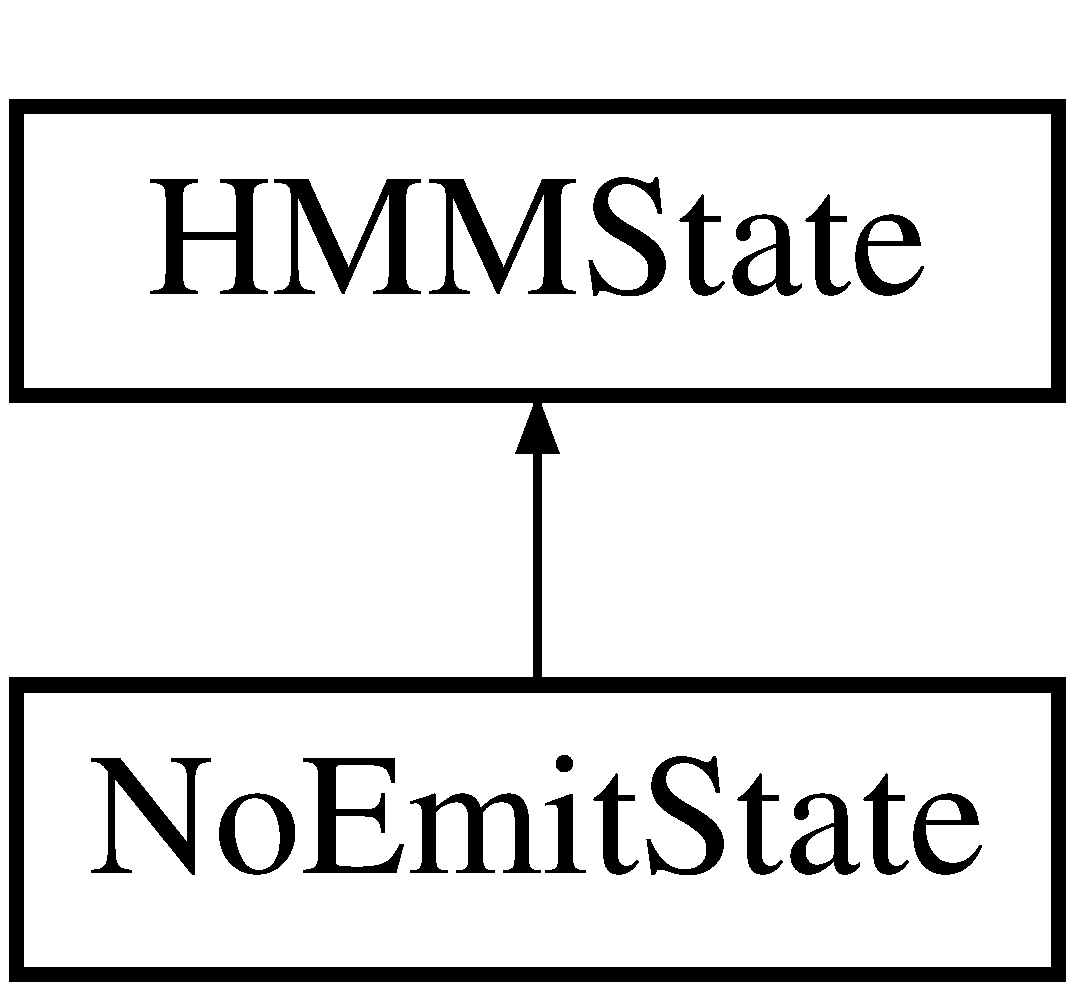
\includegraphics[height=2.000000cm]{class_no_emit_state}
\end{center}
\end{figure}
\subsection*{Public Member Functions}
\begin{DoxyCompactItemize}
\item 
\hyperlink{class_no_emit_state_a8c1093d8268fc7cedf6ac01b023f0298}{No\+Emit\+State} ()
\item 
\hyperlink{class_no_emit_state_a6d9f43ba8c4d9a21d6c5ac775eff7f54}{$\sim$\+No\+Emit\+State} ()
\item 
void \hyperlink{class_no_emit_state_acb0904c7b81e54bbfa8a995e1acd47bd}{gaussian\+Train} (int gaussian\+Num)
\item 
double \hyperlink{class_no_emit_state_a37853ca0ea0cffe47d4bacf6c9f4ea3d}{node\+Cost} (\hyperlink{class_feature}{Feature} $\ast$input\+Feature)
\item 
void \hyperlink{class_no_emit_state_a59702d5b1bb81733c2694fe1fa80a8e6}{load} (std\+::stringstream \&in, int \&\hyperlink{pro6__demo_8cpp_a923ffcfa3c56ccdba17bc4e700247d54}{gauss\+Num})
\item 
void \hyperlink{class_no_emit_state_afbe040ba5781ef6cf4f2544cb3756962}{store} (std\+::stringstream \&out)
\end{DoxyCompactItemize}
\subsection*{Additional Inherited Members}


\subsection{Constructor \& Destructor Documentation}
\hypertarget{class_no_emit_state_a8c1093d8268fc7cedf6ac01b023f0298}{\index{No\+Emit\+State@{No\+Emit\+State}!No\+Emit\+State@{No\+Emit\+State}}
\index{No\+Emit\+State@{No\+Emit\+State}!No\+Emit\+State@{No\+Emit\+State}}
\subsubsection[{No\+Emit\+State}]{\setlength{\rightskip}{0pt plus 5cm}No\+Emit\+State\+::\+No\+Emit\+State (
\begin{DoxyParamCaption}
{}
\end{DoxyParamCaption}
)\hspace{0.3cm}{\ttfamily [inline]}}}\label{class_no_emit_state_a8c1093d8268fc7cedf6ac01b023f0298}
\hypertarget{class_no_emit_state_a6d9f43ba8c4d9a21d6c5ac775eff7f54}{\index{No\+Emit\+State@{No\+Emit\+State}!````~No\+Emit\+State@{$\sim$\+No\+Emit\+State}}
\index{````~No\+Emit\+State@{$\sim$\+No\+Emit\+State}!No\+Emit\+State@{No\+Emit\+State}}
\subsubsection[{$\sim$\+No\+Emit\+State}]{\setlength{\rightskip}{0pt plus 5cm}No\+Emit\+State\+::$\sim$\+No\+Emit\+State (
\begin{DoxyParamCaption}
{}
\end{DoxyParamCaption}
)\hspace{0.3cm}{\ttfamily [inline]}}}\label{class_no_emit_state_a6d9f43ba8c4d9a21d6c5ac775eff7f54}


\subsection{Member Function Documentation}
\hypertarget{class_no_emit_state_acb0904c7b81e54bbfa8a995e1acd47bd}{\index{No\+Emit\+State@{No\+Emit\+State}!gaussian\+Train@{gaussian\+Train}}
\index{gaussian\+Train@{gaussian\+Train}!No\+Emit\+State@{No\+Emit\+State}}
\subsubsection[{gaussian\+Train}]{\setlength{\rightskip}{0pt plus 5cm}void No\+Emit\+State\+::gaussian\+Train (
\begin{DoxyParamCaption}
\item[{int}]{gaussian\+Num}
\end{DoxyParamCaption}
)\hspace{0.3cm}{\ttfamily [inline]}, {\ttfamily [virtual]}}}\label{class_no_emit_state_acb0904c7b81e54bbfa8a995e1acd47bd}


Implements \hyperlink{class_h_m_m_state_a2d42dd972a85014c0f5f9875da1eacd7}{H\+M\+M\+State}.

\hypertarget{class_no_emit_state_a59702d5b1bb81733c2694fe1fa80a8e6}{\index{No\+Emit\+State@{No\+Emit\+State}!load@{load}}
\index{load@{load}!No\+Emit\+State@{No\+Emit\+State}}
\subsubsection[{load}]{\setlength{\rightskip}{0pt plus 5cm}void No\+Emit\+State\+::load (
\begin{DoxyParamCaption}
\item[{std\+::stringstream \&}]{in, }
\item[{int \&}]{gauss\+Num}
\end{DoxyParamCaption}
)\hspace{0.3cm}{\ttfamily [inline]}, {\ttfamily [virtual]}}}\label{class_no_emit_state_a59702d5b1bb81733c2694fe1fa80a8e6}


Implements \hyperlink{class_h_m_m_state_ad5d14bf058b8fc39e07319fabebe09ee}{H\+M\+M\+State}.

\hypertarget{class_no_emit_state_a37853ca0ea0cffe47d4bacf6c9f4ea3d}{\index{No\+Emit\+State@{No\+Emit\+State}!node\+Cost@{node\+Cost}}
\index{node\+Cost@{node\+Cost}!No\+Emit\+State@{No\+Emit\+State}}
\subsubsection[{node\+Cost}]{\setlength{\rightskip}{0pt plus 5cm}double No\+Emit\+State\+::node\+Cost (
\begin{DoxyParamCaption}
\item[{{\bf Feature} $\ast$}]{input\+Feature}
\end{DoxyParamCaption}
)\hspace{0.3cm}{\ttfamily [inline]}, {\ttfamily [virtual]}}}\label{class_no_emit_state_a37853ca0ea0cffe47d4bacf6c9f4ea3d}


Implements \hyperlink{class_h_m_m_state_a84ad1899239f79257837e6d77cc4f242}{H\+M\+M\+State}.

\hypertarget{class_no_emit_state_afbe040ba5781ef6cf4f2544cb3756962}{\index{No\+Emit\+State@{No\+Emit\+State}!store@{store}}
\index{store@{store}!No\+Emit\+State@{No\+Emit\+State}}
\subsubsection[{store}]{\setlength{\rightskip}{0pt plus 5cm}void No\+Emit\+State\+::store (
\begin{DoxyParamCaption}
\item[{std\+::stringstream \&}]{out}
\end{DoxyParamCaption}
)\hspace{0.3cm}{\ttfamily [inline]}, {\ttfamily [virtual]}}}\label{class_no_emit_state_afbe040ba5781ef6cf4f2544cb3756962}


Implements \hyperlink{class_h_m_m_state_ab12116fc28ade677ee79ff13b4577ea6}{H\+M\+M\+State}.



The documentation for this class was generated from the following file\+:\begin{DoxyCompactItemize}
\item 
src/\+Feature/\hyperlink{_no_emit_state_8h}{No\+Emit\+State.\+h}\end{DoxyCompactItemize}

\hypertarget{struct_feature_extractor_1_1padding__task__info}{\section{Feature\+Extractor\+:\+:padding\+\_\+task\+\_\+info Struct Reference}
\label{struct_feature_extractor_1_1padding__task__info}\index{Feature\+Extractor\+::padding\+\_\+task\+\_\+info@{Feature\+Extractor\+::padding\+\_\+task\+\_\+info}}
}
\subsection*{Public Attributes}
\begin{DoxyCompactItemize}
\item 
std\+::vector$<$ double $>$ $\ast$ \hyperlink{struct_feature_extractor_1_1padding__task__info_a9a88478c04cf54c33f9b75830612894f}{window}
\item 
int \hyperlink{struct_feature_extractor_1_1padding__task__info_a6938d448f871a7011e161ae5514735da}{nfft}
\end{DoxyCompactItemize}


\subsection{Member Data Documentation}
\hypertarget{struct_feature_extractor_1_1padding__task__info_a6938d448f871a7011e161ae5514735da}{\index{Feature\+Extractor\+::padding\+\_\+task\+\_\+info@{Feature\+Extractor\+::padding\+\_\+task\+\_\+info}!nfft@{nfft}}
\index{nfft@{nfft}!Feature\+Extractor\+::padding\+\_\+task\+\_\+info@{Feature\+Extractor\+::padding\+\_\+task\+\_\+info}}
\subsubsection[{nfft}]{\setlength{\rightskip}{0pt plus 5cm}int Feature\+Extractor\+::padding\+\_\+task\+\_\+info\+::nfft}}\label{struct_feature_extractor_1_1padding__task__info_a6938d448f871a7011e161ae5514735da}
\hypertarget{struct_feature_extractor_1_1padding__task__info_a9a88478c04cf54c33f9b75830612894f}{\index{Feature\+Extractor\+::padding\+\_\+task\+\_\+info@{Feature\+Extractor\+::padding\+\_\+task\+\_\+info}!window@{window}}
\index{window@{window}!Feature\+Extractor\+::padding\+\_\+task\+\_\+info@{Feature\+Extractor\+::padding\+\_\+task\+\_\+info}}
\subsubsection[{window}]{\setlength{\rightskip}{0pt plus 5cm}std\+::vector$<$double$>$$\ast$ Feature\+Extractor\+::padding\+\_\+task\+\_\+info\+::window}}\label{struct_feature_extractor_1_1padding__task__info_a9a88478c04cf54c33f9b75830612894f}


The documentation for this struct was generated from the following file\+:\begin{DoxyCompactItemize}
\item 
src/\+Feature/\hyperlink{_feature_extractor_8h}{Feature\+Extractor.\+h}\end{DoxyCompactItemize}

\hypertarget{class_parse_graph}{\section{Parse\+Graph Class Reference}
\label{class_parse_graph}\index{Parse\+Graph@{Parse\+Graph}}
}


{\ttfamily \#include $<$parse\+Graph.\+h$>$}

\subsection*{Public Member Functions}
\begin{DoxyCompactItemize}
\item 
\hyperlink{class_parse_graph_ac028f7a94597ca2ac3b01e10ba266935}{Parse\+Graph} ()
\item 
\hyperlink{class_parse_graph_a6becedb93dd1914f77a4aea19a0b8d28}{$\sim$\+Parse\+Graph} ()
\item 
void \hyperlink{class_parse_graph_a2ace10c27cbb5a41b5a027d61c5cdfd2}{parse\+Graph} (const char $\ast$filename)
\item 
void \hyperlink{class_parse_graph_a0c66bf675ab6613f0124695e8ff9a70d}{parse\+Seq\+Str} (const std\+::string \&seq\+Str)
\item 
void \hyperlink{class_parse_graph_a4aefd95b81fbfcb690569ef10c5860ff}{dump} (std\+::ostream \&out) const 
\item 
int \hyperlink{class_parse_graph_a6fe380fb738f8e98d9cb9c8a1277b13f}{size} () const 
\item 
const \hyperlink{struct_graph_edge}{Graph\+Edge} \& \hyperlink{class_parse_graph_adeac9d18aed9c028ded376dc55940da8}{operator\mbox{[}$\,$\mbox{]}} (int idx) const 
\end{DoxyCompactItemize}
\subsection*{Static Public Member Functions}
\begin{DoxyCompactItemize}
\item 
static void \hyperlink{class_parse_graph_ad5cc3b524addc21852012302eecee7ad}{dump\+Seq\+Str2\+Vec} (const std\+::string \&seq\+Str, std\+::vector$<$ std\+::string $>$ \&res)
\end{DoxyCompactItemize}
\subsection*{Private Attributes}
\begin{DoxyCompactItemize}
\item 
std\+::vector$<$ \hyperlink{struct_graph_edge}{Graph\+Edge} $>$ \hyperlink{class_parse_graph_a65a7410819c36f48c0c5ebf787f57afb}{edges}
\end{DoxyCompactItemize}


\subsection{Constructor \& Destructor Documentation}
\hypertarget{class_parse_graph_ac028f7a94597ca2ac3b01e10ba266935}{\index{Parse\+Graph@{Parse\+Graph}!Parse\+Graph@{Parse\+Graph}}
\index{Parse\+Graph@{Parse\+Graph}!Parse\+Graph@{Parse\+Graph}}
\subsubsection[{Parse\+Graph}]{\setlength{\rightskip}{0pt plus 5cm}Parse\+Graph\+::\+Parse\+Graph (
\begin{DoxyParamCaption}
{}
\end{DoxyParamCaption}
)\hspace{0.3cm}{\ttfamily [inline]}}}\label{class_parse_graph_ac028f7a94597ca2ac3b01e10ba266935}
\hypertarget{class_parse_graph_a6becedb93dd1914f77a4aea19a0b8d28}{\index{Parse\+Graph@{Parse\+Graph}!````~Parse\+Graph@{$\sim$\+Parse\+Graph}}
\index{````~Parse\+Graph@{$\sim$\+Parse\+Graph}!Parse\+Graph@{Parse\+Graph}}
\subsubsection[{$\sim$\+Parse\+Graph}]{\setlength{\rightskip}{0pt plus 5cm}Parse\+Graph\+::$\sim$\+Parse\+Graph (
\begin{DoxyParamCaption}
{}
\end{DoxyParamCaption}
)\hspace{0.3cm}{\ttfamily [inline]}}}\label{class_parse_graph_a6becedb93dd1914f77a4aea19a0b8d28}


\subsection{Member Function Documentation}
\hypertarget{class_parse_graph_a4aefd95b81fbfcb690569ef10c5860ff}{\index{Parse\+Graph@{Parse\+Graph}!dump@{dump}}
\index{dump@{dump}!Parse\+Graph@{Parse\+Graph}}
\subsubsection[{dump}]{\setlength{\rightskip}{0pt plus 5cm}void Parse\+Graph\+::dump (
\begin{DoxyParamCaption}
\item[{std\+::ostream \&}]{out}
\end{DoxyParamCaption}
) const}}\label{class_parse_graph_a4aefd95b81fbfcb690569ef10c5860ff}
\hypertarget{class_parse_graph_ad5cc3b524addc21852012302eecee7ad}{\index{Parse\+Graph@{Parse\+Graph}!dump\+Seq\+Str2\+Vec@{dump\+Seq\+Str2\+Vec}}
\index{dump\+Seq\+Str2\+Vec@{dump\+Seq\+Str2\+Vec}!Parse\+Graph@{Parse\+Graph}}
\subsubsection[{dump\+Seq\+Str2\+Vec}]{\setlength{\rightskip}{0pt plus 5cm}void Parse\+Graph\+::dump\+Seq\+Str2\+Vec (
\begin{DoxyParamCaption}
\item[{const std\+::string \&}]{seq\+Str, }
\item[{std\+::vector$<$ std\+::string $>$ \&}]{res}
\end{DoxyParamCaption}
)\hspace{0.3cm}{\ttfamily [static]}}}\label{class_parse_graph_ad5cc3b524addc21852012302eecee7ad}
\hypertarget{class_parse_graph_adeac9d18aed9c028ded376dc55940da8}{\index{Parse\+Graph@{Parse\+Graph}!operator\mbox{[}$\,$\mbox{]}@{operator[]}}
\index{operator\mbox{[}$\,$\mbox{]}@{operator[]}!Parse\+Graph@{Parse\+Graph}}
\subsubsection[{operator[]}]{\setlength{\rightskip}{0pt plus 5cm}const {\bf Graph\+Edge}\& Parse\+Graph\+::operator\mbox{[}$\,$\mbox{]} (
\begin{DoxyParamCaption}
\item[{int}]{idx}
\end{DoxyParamCaption}
) const\hspace{0.3cm}{\ttfamily [inline]}}}\label{class_parse_graph_adeac9d18aed9c028ded376dc55940da8}
\hypertarget{class_parse_graph_a2ace10c27cbb5a41b5a027d61c5cdfd2}{\index{Parse\+Graph@{Parse\+Graph}!parse\+Graph@{parse\+Graph}}
\index{parse\+Graph@{parse\+Graph}!Parse\+Graph@{Parse\+Graph}}
\subsubsection[{parse\+Graph}]{\setlength{\rightskip}{0pt plus 5cm}void Parse\+Graph\+::parse\+Graph (
\begin{DoxyParamCaption}
\item[{const char $\ast$}]{filename}
\end{DoxyParamCaption}
)}}\label{class_parse_graph_a2ace10c27cbb5a41b5a027d61c5cdfd2}
\hypertarget{class_parse_graph_a0c66bf675ab6613f0124695e8ff9a70d}{\index{Parse\+Graph@{Parse\+Graph}!parse\+Seq\+Str@{parse\+Seq\+Str}}
\index{parse\+Seq\+Str@{parse\+Seq\+Str}!Parse\+Graph@{Parse\+Graph}}
\subsubsection[{parse\+Seq\+Str}]{\setlength{\rightskip}{0pt plus 5cm}void Parse\+Graph\+::parse\+Seq\+Str (
\begin{DoxyParamCaption}
\item[{const std\+::string \&}]{seq\+Str}
\end{DoxyParamCaption}
)}}\label{class_parse_graph_a0c66bf675ab6613f0124695e8ff9a70d}
\hypertarget{class_parse_graph_a6fe380fb738f8e98d9cb9c8a1277b13f}{\index{Parse\+Graph@{Parse\+Graph}!size@{size}}
\index{size@{size}!Parse\+Graph@{Parse\+Graph}}
\subsubsection[{size}]{\setlength{\rightskip}{0pt plus 5cm}int Parse\+Graph\+::size (
\begin{DoxyParamCaption}
{}
\end{DoxyParamCaption}
) const\hspace{0.3cm}{\ttfamily [inline]}}}\label{class_parse_graph_a6fe380fb738f8e98d9cb9c8a1277b13f}


\subsection{Member Data Documentation}
\hypertarget{class_parse_graph_a65a7410819c36f48c0c5ebf787f57afb}{\index{Parse\+Graph@{Parse\+Graph}!edges@{edges}}
\index{edges@{edges}!Parse\+Graph@{Parse\+Graph}}
\subsubsection[{edges}]{\setlength{\rightskip}{0pt plus 5cm}std\+::vector$<$ {\bf Graph\+Edge} $>$ Parse\+Graph\+::edges\hspace{0.3cm}{\ttfamily [private]}}}\label{class_parse_graph_a65a7410819c36f48c0c5ebf787f57afb}


The documentation for this class was generated from the following files\+:\begin{DoxyCompactItemize}
\item 
src/\+Graph/\hyperlink{parse_graph_8h}{parse\+Graph.\+h}\item 
src/\+Graph/\hyperlink{parse_graph_8cpp}{parse\+Graph.\+cpp}\end{DoxyCompactItemize}

\hypertarget{struct_path}{\section{Path Struct Reference}
\label{struct_path}\index{Path@{Path}}
}


{\ttfamily \#include $<$path.\+h$>$}

\subsection*{Public Member Functions}
\begin{DoxyCompactItemize}
\item 
\hyperlink{struct_path_af26cfab021ddf49af73da3b2beca85ac}{Path} ()
\item 
\hyperlink{struct_path_a6d10e7e278f139f9a9bb331c6663637f}{Path} (int m)
\item 
void \hyperlink{struct_path_a88122b492a3c550f03b66b4d91198c5d}{print} ()
\item 
void \hyperlink{struct_path_a9c8285042c96f9e46b4b1580a9f7fbf7}{set\+Max\+Len} (int m)
\item 
void \hyperlink{struct_path_a8ca4768f44455b55e3cd8b02e0a50c35}{add} (\hyperlink{path_8h_a49eb6ac4643553d04b85c70646c6786d}{D\+I\+R} \hyperlink{readhtk_8m_aaccc9105df5383111407fd5b41255e23}{t})
\item 
\hyperlink{struct_path_a141da9ff89c85e0ba410b5a73864c267}{$\sim$\+Path} ()
\item 
\hyperlink{struct_path_af26cfab021ddf49af73da3b2beca85ac}{Path} ()
\item 
void \hyperlink{struct_path_a76d7e0cfeec9a365d9d2cdb4cf94386c}{init} (int \hyperlink{struct_path_a3020a9bdb6f4181571b616468577627a}{size})
\item 
void \hyperlink{struct_path_a01b0c21c26eca649f0d45c5403a03a09}{create} (int \hyperlink{rastafilt_8m_ae1674a322a8fdaf497b48f50e749ddac}{x}, int \hyperlink{rastafilt_8m_a86d95dcd476896268e6f41d4bcc8c2fc}{y}, int px, int py)
\item 
void \hyperlink{struct_path_a27c8f61321579810b2b6267415825f29}{print} (int \hyperlink{rastafilt_8m_ae1674a322a8fdaf497b48f50e749ddac}{x}, int \hyperlink{rastafilt_8m_a86d95dcd476896268e6f41d4bcc8c2fc}{y})
\end{DoxyCompactItemize}
\subsection*{Public Attributes}
\begin{DoxyCompactItemize}
\item 
int \hyperlink{struct_path_a3495299d7cfe9c09f4559f3bf33d58e9}{len}
\item 
\hyperlink{path_8h_a49eb6ac4643553d04b85c70646c6786d}{D\+I\+R} $\ast$ \hyperlink{struct_path_a48a4abe4c0c17bd705d650ac2e4fea98}{dir}
\item 
int $\ast$ \hyperlink{struct_path_add6f2732f31960bd9be2e6dda9f7d9ab}{val}
\item 
std\+::map$<$ int, int $>$ \hyperlink{struct_path_a3ef5985a151fd31af4b3510ed08129fc}{path}
\item 
int \hyperlink{struct_path_a3020a9bdb6f4181571b616468577627a}{size}
\item 
bool \hyperlink{struct_path_a44f7e932bded8d8eef1febd440c9516a}{use}
\end{DoxyCompactItemize}


\subsection{Constructor \& Destructor Documentation}
\hypertarget{struct_path_af26cfab021ddf49af73da3b2beca85ac}{\index{Path@{Path}!Path@{Path}}
\index{Path@{Path}!Path@{Path}}
\subsubsection[{Path}]{\setlength{\rightskip}{0pt plus 5cm}Path\+::\+Path (
\begin{DoxyParamCaption}
{}
\end{DoxyParamCaption}
)\hspace{0.3cm}{\ttfamily [inline]}}}\label{struct_path_af26cfab021ddf49af73da3b2beca85ac}
\hypertarget{struct_path_a6d10e7e278f139f9a9bb331c6663637f}{\index{Path@{Path}!Path@{Path}}
\index{Path@{Path}!Path@{Path}}
\subsubsection[{Path}]{\setlength{\rightskip}{0pt plus 5cm}Path\+::\+Path (
\begin{DoxyParamCaption}
\item[{int}]{m}
\end{DoxyParamCaption}
)\hspace{0.3cm}{\ttfamily [inline]}}}\label{struct_path_a6d10e7e278f139f9a9bb331c6663637f}
\hypertarget{struct_path_a141da9ff89c85e0ba410b5a73864c267}{\index{Path@{Path}!````~Path@{$\sim$\+Path}}
\index{````~Path@{$\sim$\+Path}!Path@{Path}}
\subsubsection[{$\sim$\+Path}]{\setlength{\rightskip}{0pt plus 5cm}Path\+::$\sim$\+Path (
\begin{DoxyParamCaption}
{}
\end{DoxyParamCaption}
)\hspace{0.3cm}{\ttfamily [inline]}}}\label{struct_path_a141da9ff89c85e0ba410b5a73864c267}
\hypertarget{struct_path_af26cfab021ddf49af73da3b2beca85ac}{\index{Path@{Path}!Path@{Path}}
\index{Path@{Path}!Path@{Path}}
\subsubsection[{Path}]{\setlength{\rightskip}{0pt plus 5cm}Path\+::\+Path (
\begin{DoxyParamCaption}
{}
\end{DoxyParamCaption}
)\hspace{0.3cm}{\ttfamily [inline]}}}\label{struct_path_af26cfab021ddf49af73da3b2beca85ac}


\subsection{Member Function Documentation}
\hypertarget{struct_path_a8ca4768f44455b55e3cd8b02e0a50c35}{\index{Path@{Path}!add@{add}}
\index{add@{add}!Path@{Path}}
\subsubsection[{add}]{\setlength{\rightskip}{0pt plus 5cm}void Path\+::add (
\begin{DoxyParamCaption}
\item[{{\bf D\+I\+R}}]{t}
\end{DoxyParamCaption}
)\hspace{0.3cm}{\ttfamily [inline]}}}\label{struct_path_a8ca4768f44455b55e3cd8b02e0a50c35}
\hypertarget{struct_path_a01b0c21c26eca649f0d45c5403a03a09}{\index{Path@{Path}!create@{create}}
\index{create@{create}!Path@{Path}}
\subsubsection[{create}]{\setlength{\rightskip}{0pt plus 5cm}void Path\+::create (
\begin{DoxyParamCaption}
\item[{int}]{x, }
\item[{int}]{y, }
\item[{int}]{px, }
\item[{int}]{py}
\end{DoxyParamCaption}
)\hspace{0.3cm}{\ttfamily [inline]}}}\label{struct_path_a01b0c21c26eca649f0d45c5403a03a09}
\hypertarget{struct_path_a76d7e0cfeec9a365d9d2cdb4cf94386c}{\index{Path@{Path}!init@{init}}
\index{init@{init}!Path@{Path}}
\subsubsection[{init}]{\setlength{\rightskip}{0pt plus 5cm}void Path\+::init (
\begin{DoxyParamCaption}
\item[{int}]{size}
\end{DoxyParamCaption}
)\hspace{0.3cm}{\ttfamily [inline]}}}\label{struct_path_a76d7e0cfeec9a365d9d2cdb4cf94386c}
\hypertarget{struct_path_a27c8f61321579810b2b6267415825f29}{\index{Path@{Path}!print@{print}}
\index{print@{print}!Path@{Path}}
\subsubsection[{print}]{\setlength{\rightskip}{0pt plus 5cm}void Path\+::print (
\begin{DoxyParamCaption}
\item[{int}]{x, }
\item[{int}]{y}
\end{DoxyParamCaption}
)\hspace{0.3cm}{\ttfamily [inline]}}}\label{struct_path_a27c8f61321579810b2b6267415825f29}
\hypertarget{struct_path_a88122b492a3c550f03b66b4d91198c5d}{\index{Path@{Path}!print@{print}}
\index{print@{print}!Path@{Path}}
\subsubsection[{print}]{\setlength{\rightskip}{0pt plus 5cm}void Path\+::print (
\begin{DoxyParamCaption}
{}
\end{DoxyParamCaption}
)\hspace{0.3cm}{\ttfamily [inline]}}}\label{struct_path_a88122b492a3c550f03b66b4d91198c5d}
\hypertarget{struct_path_a9c8285042c96f9e46b4b1580a9f7fbf7}{\index{Path@{Path}!set\+Max\+Len@{set\+Max\+Len}}
\index{set\+Max\+Len@{set\+Max\+Len}!Path@{Path}}
\subsubsection[{set\+Max\+Len}]{\setlength{\rightskip}{0pt plus 5cm}void Path\+::set\+Max\+Len (
\begin{DoxyParamCaption}
\item[{int}]{m}
\end{DoxyParamCaption}
)\hspace{0.3cm}{\ttfamily [inline]}}}\label{struct_path_a9c8285042c96f9e46b4b1580a9f7fbf7}


\subsection{Member Data Documentation}
\hypertarget{struct_path_a48a4abe4c0c17bd705d650ac2e4fea98}{\index{Path@{Path}!dir@{dir}}
\index{dir@{dir}!Path@{Path}}
\subsubsection[{dir}]{\setlength{\rightskip}{0pt plus 5cm}{\bf D\+I\+R}$\ast$ Path\+::dir}}\label{struct_path_a48a4abe4c0c17bd705d650ac2e4fea98}
\hypertarget{struct_path_a3495299d7cfe9c09f4559f3bf33d58e9}{\index{Path@{Path}!len@{len}}
\index{len@{len}!Path@{Path}}
\subsubsection[{len}]{\setlength{\rightskip}{0pt plus 5cm}int Path\+::len}}\label{struct_path_a3495299d7cfe9c09f4559f3bf33d58e9}
\hypertarget{struct_path_a3ef5985a151fd31af4b3510ed08129fc}{\index{Path@{Path}!path@{path}}
\index{path@{path}!Path@{Path}}
\subsubsection[{path}]{\setlength{\rightskip}{0pt plus 5cm}std\+::map$<$int,int$>$ Path\+::path}}\label{struct_path_a3ef5985a151fd31af4b3510ed08129fc}
\hypertarget{struct_path_a3020a9bdb6f4181571b616468577627a}{\index{Path@{Path}!size@{size}}
\index{size@{size}!Path@{Path}}
\subsubsection[{size}]{\setlength{\rightskip}{0pt plus 5cm}int Path\+::size}}\label{struct_path_a3020a9bdb6f4181571b616468577627a}
\hypertarget{struct_path_a44f7e932bded8d8eef1febd440c9516a}{\index{Path@{Path}!use@{use}}
\index{use@{use}!Path@{Path}}
\subsubsection[{use}]{\setlength{\rightskip}{0pt plus 5cm}bool Path\+::use}}\label{struct_path_a44f7e932bded8d8eef1febd440c9516a}
\hypertarget{struct_path_add6f2732f31960bd9be2e6dda9f7d9ab}{\index{Path@{Path}!val@{val}}
\index{val@{val}!Path@{Path}}
\subsubsection[{val}]{\setlength{\rightskip}{0pt plus 5cm}int$\ast$ Path\+::val}}\label{struct_path_add6f2732f31960bd9be2e6dda9f7d9ab}


The documentation for this struct was generated from the following files\+:\begin{DoxyCompactItemize}
\item 
src/\+Edit\+Distance/\hyperlink{path_8h}{path.\+h}\item 
src/\+Lex\+Tree/\hyperlink{spellcheck_8h}{spellcheck.\+h}\end{DoxyCompactItemize}

\hypertarget{class_raw_data}{\section{Raw\+Data Class Reference}
\label{class_raw_data}\index{Raw\+Data@{Raw\+Data}}
}


{\ttfamily \#include $<$Raw\+Data.\+h$>$}

\subsection*{Public Member Functions}
\begin{DoxyCompactItemize}
\item 
\hyperlink{class_raw_data_a583cd50c06a9fbaebdaaf44621401552}{Raw\+Data} ()
\item 
\hyperlink{class_raw_data_a9ebfa3736a2e278a34b169549d5efa3d}{Raw\+Data} (const \hyperlink{class_raw_data}{Raw\+Data} \&raw\+Data)
\item 
\hyperlink{class_raw_data_a214d10a81d07c892cb7b35653772e4e4}{$\sim$\+Raw\+Data} ()
\item 
void \hyperlink{class_raw_data_af1ad52746f7569118ece4f16fc8516d6}{clean} ()
\item 
bool \hyperlink{class_raw_data_a18c4c868312e7d850de4ff386e8698a0}{set\+Frame\+Num} (int f\+\_\+num)
\item 
const \hyperlink{configure__basic_8h_abf32ffaff24ba21700fbd0898b49ab02}{S\+O\+U\+N\+D\+\_\+\+D\+A\+T\+A} $\ast$ \hyperlink{class_raw_data_a166b59a84c19851aa2cd694d120d560f}{get\+Data} () const 
\item 
void \hyperlink{class_raw_data_a69101a0023281a035cd811f6858fea81}{set\+Data} (int index, \hyperlink{configure__basic_8h_abf32ffaff24ba21700fbd0898b49ab02}{S\+O\+U\+N\+D\+\_\+\+D\+A\+T\+A} \hyperlink{deltas_8m_ace9cdca9c1b355d9b321fd7f5ec2026b}{d})
\item 
bool \hyperlink{class_raw_data_af028c01fa2921829ff2f4a5e2c23da64}{append\+Block\+Data} (const \hyperlink{configure__basic_8h_abf32ffaff24ba21700fbd0898b49ab02}{S\+O\+U\+N\+D\+\_\+\+D\+A\+T\+A} $\ast$src)
\item 
void \hyperlink{class_raw_data_a003878d4445eed6fe8c21cb0d373e232}{copy\+Block\+Data} (int from, int \hyperlink{rastaplp_8m_a41c60bbfbe5db430f286f173be10a1e6}{to})
\item 
double \hyperlink{class_raw_data_a2a72d20d0fe44c15779f21d2b6f8baa9}{get\+Block\+Ave\+Energy} (int index)
\item 
bool \hyperlink{class_raw_data_a9459fcb81d0dd49a2ce8f0c164b1ffdc}{save\+Wav} (const char $\ast$file\+\_\+name)
\item 
bool \hyperlink{class_raw_data_ac6ec33dca034b3ae714f626bab48ac4a}{load\+Wav} (const char $\ast$file\+\_\+name)
\end{DoxyCompactItemize}
\subsection*{Protected Attributes}
\begin{DoxyCompactItemize}
\item 
\hyperlink{configure__basic_8h_abf32ffaff24ba21700fbd0898b49ab02}{S\+O\+U\+N\+D\+\_\+\+D\+A\+T\+A} $\ast$ \hyperlink{class_raw_data_aa59dfb6368c8d9ed49234ed129f1ed0a}{data}
\end{DoxyCompactItemize}
\subsection*{Private Member Functions}
\begin{DoxyCompactItemize}
\item 
\hyperlink{class_raw_data_aceacd6f3691e39fd73de8d774581e87c}{R\+E\+A\+D\+\_\+\+O\+N\+L\+Y\+\_\+\+D\+E\+C\+L\+A\+R\+E} (int, frame\+\_\+num, Frame\+Num)
\end{DoxyCompactItemize}


\subsection{Constructor \& Destructor Documentation}
\hypertarget{class_raw_data_a583cd50c06a9fbaebdaaf44621401552}{\index{Raw\+Data@{Raw\+Data}!Raw\+Data@{Raw\+Data}}
\index{Raw\+Data@{Raw\+Data}!Raw\+Data@{Raw\+Data}}
\subsubsection[{Raw\+Data}]{\setlength{\rightskip}{0pt plus 5cm}Raw\+Data\+::\+Raw\+Data (
\begin{DoxyParamCaption}
{}
\end{DoxyParamCaption}
)}}\label{class_raw_data_a583cd50c06a9fbaebdaaf44621401552}
\hypertarget{class_raw_data_a9ebfa3736a2e278a34b169549d5efa3d}{\index{Raw\+Data@{Raw\+Data}!Raw\+Data@{Raw\+Data}}
\index{Raw\+Data@{Raw\+Data}!Raw\+Data@{Raw\+Data}}
\subsubsection[{Raw\+Data}]{\setlength{\rightskip}{0pt plus 5cm}Raw\+Data\+::\+Raw\+Data (
\begin{DoxyParamCaption}
\item[{const {\bf Raw\+Data} \&}]{raw\+Data}
\end{DoxyParamCaption}
)}}\label{class_raw_data_a9ebfa3736a2e278a34b169549d5efa3d}
\hypertarget{class_raw_data_a214d10a81d07c892cb7b35653772e4e4}{\index{Raw\+Data@{Raw\+Data}!````~Raw\+Data@{$\sim$\+Raw\+Data}}
\index{````~Raw\+Data@{$\sim$\+Raw\+Data}!Raw\+Data@{Raw\+Data}}
\subsubsection[{$\sim$\+Raw\+Data}]{\setlength{\rightskip}{0pt plus 5cm}Raw\+Data\+::$\sim$\+Raw\+Data (
\begin{DoxyParamCaption}
{}
\end{DoxyParamCaption}
)}}\label{class_raw_data_a214d10a81d07c892cb7b35653772e4e4}


\subsection{Member Function Documentation}
\hypertarget{class_raw_data_af028c01fa2921829ff2f4a5e2c23da64}{\index{Raw\+Data@{Raw\+Data}!append\+Block\+Data@{append\+Block\+Data}}
\index{append\+Block\+Data@{append\+Block\+Data}!Raw\+Data@{Raw\+Data}}
\subsubsection[{append\+Block\+Data}]{\setlength{\rightskip}{0pt plus 5cm}bool Raw\+Data\+::append\+Block\+Data (
\begin{DoxyParamCaption}
\item[{const {\bf S\+O\+U\+N\+D\+\_\+\+D\+A\+T\+A} $\ast$}]{src}
\end{DoxyParamCaption}
)}}\label{class_raw_data_af028c01fa2921829ff2f4a5e2c23da64}
\hypertarget{class_raw_data_af1ad52746f7569118ece4f16fc8516d6}{\index{Raw\+Data@{Raw\+Data}!clean@{clean}}
\index{clean@{clean}!Raw\+Data@{Raw\+Data}}
\subsubsection[{clean}]{\setlength{\rightskip}{0pt plus 5cm}void Raw\+Data\+::clean (
\begin{DoxyParamCaption}
{}
\end{DoxyParamCaption}
)}}\label{class_raw_data_af1ad52746f7569118ece4f16fc8516d6}
\hypertarget{class_raw_data_a003878d4445eed6fe8c21cb0d373e232}{\index{Raw\+Data@{Raw\+Data}!copy\+Block\+Data@{copy\+Block\+Data}}
\index{copy\+Block\+Data@{copy\+Block\+Data}!Raw\+Data@{Raw\+Data}}
\subsubsection[{copy\+Block\+Data}]{\setlength{\rightskip}{0pt plus 5cm}void Raw\+Data\+::copy\+Block\+Data (
\begin{DoxyParamCaption}
\item[{int}]{from, }
\item[{int}]{to}
\end{DoxyParamCaption}
)}}\label{class_raw_data_a003878d4445eed6fe8c21cb0d373e232}
\hypertarget{class_raw_data_a2a72d20d0fe44c15779f21d2b6f8baa9}{\index{Raw\+Data@{Raw\+Data}!get\+Block\+Ave\+Energy@{get\+Block\+Ave\+Energy}}
\index{get\+Block\+Ave\+Energy@{get\+Block\+Ave\+Energy}!Raw\+Data@{Raw\+Data}}
\subsubsection[{get\+Block\+Ave\+Energy}]{\setlength{\rightskip}{0pt plus 5cm}double Raw\+Data\+::get\+Block\+Ave\+Energy (
\begin{DoxyParamCaption}
\item[{int}]{index}
\end{DoxyParamCaption}
)}}\label{class_raw_data_a2a72d20d0fe44c15779f21d2b6f8baa9}
\hypertarget{class_raw_data_a166b59a84c19851aa2cd694d120d560f}{\index{Raw\+Data@{Raw\+Data}!get\+Data@{get\+Data}}
\index{get\+Data@{get\+Data}!Raw\+Data@{Raw\+Data}}
\subsubsection[{get\+Data}]{\setlength{\rightskip}{0pt plus 5cm}const {\bf S\+O\+U\+N\+D\+\_\+\+D\+A\+T\+A} $\ast$ Raw\+Data\+::get\+Data (
\begin{DoxyParamCaption}
{}
\end{DoxyParamCaption}
) const}}\label{class_raw_data_a166b59a84c19851aa2cd694d120d560f}
\hypertarget{class_raw_data_ac6ec33dca034b3ae714f626bab48ac4a}{\index{Raw\+Data@{Raw\+Data}!load\+Wav@{load\+Wav}}
\index{load\+Wav@{load\+Wav}!Raw\+Data@{Raw\+Data}}
\subsubsection[{load\+Wav}]{\setlength{\rightskip}{0pt plus 5cm}bool Raw\+Data\+::load\+Wav (
\begin{DoxyParamCaption}
\item[{const char $\ast$}]{file\+\_\+name}
\end{DoxyParamCaption}
)}}\label{class_raw_data_ac6ec33dca034b3ae714f626bab48ac4a}
\hypertarget{class_raw_data_aceacd6f3691e39fd73de8d774581e87c}{\index{Raw\+Data@{Raw\+Data}!R\+E\+A\+D\+\_\+\+O\+N\+L\+Y\+\_\+\+D\+E\+C\+L\+A\+R\+E@{R\+E\+A\+D\+\_\+\+O\+N\+L\+Y\+\_\+\+D\+E\+C\+L\+A\+R\+E}}
\index{R\+E\+A\+D\+\_\+\+O\+N\+L\+Y\+\_\+\+D\+E\+C\+L\+A\+R\+E@{R\+E\+A\+D\+\_\+\+O\+N\+L\+Y\+\_\+\+D\+E\+C\+L\+A\+R\+E}!Raw\+Data@{Raw\+Data}}
\subsubsection[{R\+E\+A\+D\+\_\+\+O\+N\+L\+Y\+\_\+\+D\+E\+C\+L\+A\+R\+E}]{\setlength{\rightskip}{0pt plus 5cm}Raw\+Data\+::\+R\+E\+A\+D\+\_\+\+O\+N\+L\+Y\+\_\+\+D\+E\+C\+L\+A\+R\+E (
\begin{DoxyParamCaption}
\item[{int}]{, }
\item[{frame\+\_\+num}]{, }
\item[{Frame\+Num}]{}
\end{DoxyParamCaption}
)\hspace{0.3cm}{\ttfamily [private]}}}\label{class_raw_data_aceacd6f3691e39fd73de8d774581e87c}
\hypertarget{class_raw_data_a9459fcb81d0dd49a2ce8f0c164b1ffdc}{\index{Raw\+Data@{Raw\+Data}!save\+Wav@{save\+Wav}}
\index{save\+Wav@{save\+Wav}!Raw\+Data@{Raw\+Data}}
\subsubsection[{save\+Wav}]{\setlength{\rightskip}{0pt plus 5cm}bool Raw\+Data\+::save\+Wav (
\begin{DoxyParamCaption}
\item[{const char $\ast$}]{file\+\_\+name}
\end{DoxyParamCaption}
)}}\label{class_raw_data_a9459fcb81d0dd49a2ce8f0c164b1ffdc}
\hypertarget{class_raw_data_a69101a0023281a035cd811f6858fea81}{\index{Raw\+Data@{Raw\+Data}!set\+Data@{set\+Data}}
\index{set\+Data@{set\+Data}!Raw\+Data@{Raw\+Data}}
\subsubsection[{set\+Data}]{\setlength{\rightskip}{0pt plus 5cm}void Raw\+Data\+::set\+Data (
\begin{DoxyParamCaption}
\item[{int}]{index, }
\item[{{\bf S\+O\+U\+N\+D\+\_\+\+D\+A\+T\+A}}]{d}
\end{DoxyParamCaption}
)}}\label{class_raw_data_a69101a0023281a035cd811f6858fea81}
\hypertarget{class_raw_data_a18c4c868312e7d850de4ff386e8698a0}{\index{Raw\+Data@{Raw\+Data}!set\+Frame\+Num@{set\+Frame\+Num}}
\index{set\+Frame\+Num@{set\+Frame\+Num}!Raw\+Data@{Raw\+Data}}
\subsubsection[{set\+Frame\+Num}]{\setlength{\rightskip}{0pt plus 5cm}bool Raw\+Data\+::set\+Frame\+Num (
\begin{DoxyParamCaption}
\item[{int}]{f\+\_\+num}
\end{DoxyParamCaption}
)}}\label{class_raw_data_a18c4c868312e7d850de4ff386e8698a0}


\subsection{Member Data Documentation}
\hypertarget{class_raw_data_aa59dfb6368c8d9ed49234ed129f1ed0a}{\index{Raw\+Data@{Raw\+Data}!data@{data}}
\index{data@{data}!Raw\+Data@{Raw\+Data}}
\subsubsection[{data}]{\setlength{\rightskip}{0pt plus 5cm}{\bf S\+O\+U\+N\+D\+\_\+\+D\+A\+T\+A}$\ast$ Raw\+Data\+::data\hspace{0.3cm}{\ttfamily [protected]}}}\label{class_raw_data_aa59dfb6368c8d9ed49234ed129f1ed0a}


The documentation for this class was generated from the following files\+:\begin{DoxyCompactItemize}
\item 
src/data/\hyperlink{_raw_data_8h}{Raw\+Data.\+h}\item 
src/data/\hyperlink{_raw_data_8cpp}{Raw\+Data.\+cpp}\item 
src/data/\hyperlink{_raw_data_file_8cpp}{Raw\+Data\+File.\+cpp}\end{DoxyCompactItemize}

\hypertarget{struct_seq_edge}{\section{Seq\+Edge Struct Reference}
\label{struct_seq_edge}\index{Seq\+Edge@{Seq\+Edge}}
}


{\ttfamily \#include $<$Seq\+Model.\+h$>$}

\subsection*{Public Attributes}
\begin{DoxyCompactItemize}
\item 
int \hyperlink{struct_seq_edge_a818e5eebfe2b1c574481270feff3eb03}{to}
\item 
int \hyperlink{struct_seq_edge_aa862cd7c6fd2d8b6bc4a48766bc1b4f2}{next}
\item 
double \hyperlink{struct_seq_edge_a7bf5b4558efd51b94a4dd4c80a2294bd}{cost}
\end{DoxyCompactItemize}


\subsection{Member Data Documentation}
\hypertarget{struct_seq_edge_a7bf5b4558efd51b94a4dd4c80a2294bd}{\index{Seq\+Edge@{Seq\+Edge}!cost@{cost}}
\index{cost@{cost}!Seq\+Edge@{Seq\+Edge}}
\subsubsection[{cost}]{\setlength{\rightskip}{0pt plus 5cm}double Seq\+Edge\+::cost}}\label{struct_seq_edge_a7bf5b4558efd51b94a4dd4c80a2294bd}
\hypertarget{struct_seq_edge_aa862cd7c6fd2d8b6bc4a48766bc1b4f2}{\index{Seq\+Edge@{Seq\+Edge}!next@{next}}
\index{next@{next}!Seq\+Edge@{Seq\+Edge}}
\subsubsection[{next}]{\setlength{\rightskip}{0pt plus 5cm}int Seq\+Edge\+::next}}\label{struct_seq_edge_aa862cd7c6fd2d8b6bc4a48766bc1b4f2}
\hypertarget{struct_seq_edge_a818e5eebfe2b1c574481270feff3eb03}{\index{Seq\+Edge@{Seq\+Edge}!to@{to}}
\index{to@{to}!Seq\+Edge@{Seq\+Edge}}
\subsubsection[{to}]{\setlength{\rightskip}{0pt plus 5cm}int Seq\+Edge\+::to}}\label{struct_seq_edge_a818e5eebfe2b1c574481270feff3eb03}


The documentation for this struct was generated from the following file\+:\begin{DoxyCompactItemize}
\item 
src/\+Feature/\hyperlink{_seq_model_8h}{Seq\+Model.\+h}\end{DoxyCompactItemize}

\hypertarget{class_seq_model}{\section{Seq\+Model Class Reference}
\label{class_seq_model}\index{Seq\+Model@{Seq\+Model}}
}


{\ttfamily \#include $<$Seq\+Model.\+h$>$}

\subsection*{Public Types}
\begin{DoxyCompactItemize}
\item 
enum \hyperlink{class_seq_model_a145b769692f03811a15c5289fe77da42}{S\+E\+Q\+\_\+\+D\+T\+W\+\_\+\+P\+A\+T\+H\+\_\+\+T\+Y\+P\+E} \{ \hyperlink{class_seq_model_a145b769692f03811a15c5289fe77da42ae15b7c3ac3eac793a9b988649f728d12}{N\+O\+\_\+\+R\+E\+C\+O\+R\+D}, 
\hyperlink{class_seq_model_a145b769692f03811a15c5289fe77da42a0ed418410acf105f3baf2ccbfbc4a5c4}{F\+U\+L\+L\+\_\+\+P\+A\+T\+H}, 
\hyperlink{class_seq_model_a145b769692f03811a15c5289fe77da42a4e15f646c0c498e155c24f183dbfb6fb}{B\+A\+C\+K\+\_\+\+P\+T\+R}
 \}
\end{DoxyCompactItemize}
\subsection*{Public Member Functions}
\begin{DoxyCompactItemize}
\item 
\hyperlink{class_seq_model_aeac29571be1c65086f11a5bea3a517d8}{Seq\+Model} ()
\item 
\hyperlink{class_seq_model_a99bb121085e7008eed41363f83d25118}{$\sim$\+Seq\+Model} ()
\item 
void \hyperlink{class_seq_model_abf7146e3c63cc7087cb4d6cbf92be2b3}{build\+Model} (const \hyperlink{class_parse_graph}{Parse\+Graph} \&graph, std\+::map$<$ std\+::string, \hyperlink{class_h_m_m_automaton}{H\+M\+M\+Automaton} $\ast$ $>$ \&automatons)
\item 
void \hyperlink{class_seq_model_a4bba459d7daff3d098780ac09e4a6a85}{refresh\+Edges} (const \hyperlink{class_parse_graph}{Parse\+Graph} \&graph, std\+::map$<$ std\+::string, \hyperlink{class_h_m_m_automaton}{H\+M\+M\+Automaton} $\ast$ $>$ \&automatons)
\item 
void \hyperlink{class_seq_model_a93b6a99e725800de1714e2501066b116}{recognition} (\hyperlink{class_wave_feature_o_p}{Wave\+Feature\+O\+P} \&input, std\+::vector$<$ std\+::string $>$ \&res, \hyperlink{class_seq_model_a145b769692f03811a15c5289fe77da42}{S\+E\+Q\+\_\+\+D\+T\+W\+\_\+\+P\+A\+T\+H\+\_\+\+T\+Y\+P\+E} \hyperlink{class_seq_model_afa1904812bb4a3363960db559983e195}{path\+\_\+type}=\hyperlink{class_seq_model_a145b769692f03811a15c5289fe77da42a4e15f646c0c498e155c24f183dbfb6fb}{B\+A\+C\+K\+\_\+\+P\+T\+R})
\item 
void \hyperlink{class_seq_model_aa3c44f8d03a4fec7222f878e0dd67ece}{re\+Segment} (\hyperlink{class_wave_feature_o_p}{Wave\+Feature\+O\+P} \&input, int template\+Idx)
\item 
void \hyperlink{class_seq_model_a0ba1f75784a7f949494054cfa929a728}{close} ()
\item 
void \hyperlink{class_seq_model_a06f6db60f7c9e093d75bd633ef4b198f}{dump\+Dot} (std\+::ostream \&out)
\item 
void \hyperlink{class_seq_model_a9d5e640836a004833610f04ef46cddb6}{set\+Beam} (double thr)
\end{DoxyCompactItemize}
\subsection*{Private Member Functions}
\begin{DoxyCompactItemize}
\item 
void \hyperlink{class_seq_model_a4a03d96abdd4613da32678d76ae49dc3}{refresh\+Edge} (const \hyperlink{struct_graph_edge}{Graph\+Edge} \&simple\+Edge, std\+::map$<$ std\+::string, \hyperlink{class_h_m_m_automaton}{H\+M\+M\+Automaton} $\ast$ $>$ \&automatons, int \&edge\+Cnt, int \&state\+Cnt, int \&non\+Emit\+Edge\+Cnt)
\item 
void \hyperlink{class_seq_model_abb7d93bff32d26447ec280c229e055aa}{refresh\+Edge} (std\+::vector$<$ \hyperlink{struct_seq_edge}{Seq\+Edge} $>$ \&\hyperlink{class_seq_model_ab293b1600e51e35d49bc33a45f74dd9d}{edges}, int from, int \hyperlink{rastaplp_8m_a41c60bbfbe5db430f286f173be10a1e6}{to}, double cost, int \&edge\+Cnt)
\item 
int \hyperlink{class_seq_model_aeb9f0de9dbfb5bf87ef91252af0c99c8}{refresh\+Node} (const \hyperlink{class_h_m_m_automaton}{H\+M\+M\+Automaton} \&automaton, int state\+I\+D, int \&state\+Cnt, const std\+::string \&word)
\item 
void \hyperlink{class_seq_model_abfc5affef293313a9caaf8f221e6282b}{init\+N\+O\+Emit\+States} (const \hyperlink{class_parse_graph}{Parse\+Graph} \&graph)
\item 
void \hyperlink{class_seq_model_ab783695b9217c3bbc7f930a492a729e8}{dtw} (\hyperlink{class_wave_feature_o_p}{Wave\+Feature\+O\+P} \&wav, \hyperlink{class_seq_model_a145b769692f03811a15c5289fe77da42}{S\+E\+Q\+\_\+\+D\+T\+W\+\_\+\+P\+A\+T\+H\+\_\+\+T\+Y\+P\+E} \hyperlink{class_seq_model_afa1904812bb4a3363960db559983e195}{path\+\_\+type})
\item 
int \hyperlink{class_seq_model_af2e990d1fd01d2a297733afe9bd608dd}{get\+Roll\+Idx} (int column\+Idx)
\item 
void \hyperlink{class_seq_model_a0cc11091ec47eaf08272fa7d8ce7a0ac}{set\+Path\+Type} (\hyperlink{class_seq_model_a145b769692f03811a15c5289fe77da42}{S\+E\+Q\+\_\+\+D\+T\+W\+\_\+\+P\+A\+T\+H\+\_\+\+T\+Y\+P\+E} \hyperlink{class_seq_model_afa1904812bb4a3363960db559983e195}{path\+\_\+type})
\item 
double \hyperlink{class_seq_model_a5bdca555363833c1877b9967206a6289}{forward\+Column} (\hyperlink{struct_dtw___column___link}{Dtw\+\_\+\+Column\+\_\+\+Link} $\ast$link, \hyperlink{class_wave_feature_o_p}{Wave\+Feature\+O\+P} \&wav, int column\+Idx, double \hyperlink{rawdtw_8cpp_afcfbedec6ebde62c6a091ce335836ef1}{threshold})
\item 
void \hyperlink{class_seq_model_ac008d90549bd9f165a576c6f2dd21c6b}{try\+Update} (\hyperlink{struct_dtw___column___link}{Dtw\+\_\+\+Column\+\_\+\+Link} $\ast$link, int column\+Idx, int pre\+State\+I\+D, int state\+I\+D, double new\+Cost)
\item 
void \hyperlink{class_seq_model_a09ed709bb828242d2741f23dbf04a094}{try\+Forward\+To\+Star} (\hyperlink{struct_dtw___column___link}{Dtw\+\_\+\+Column\+\_\+\+Link} $\ast$link, int column\+Idx, int state\+I\+D, double pre\+Cost)
\item 
void \hyperlink{class_seq_model_a270c77892a0af88e65870411836460cc}{prepare\+Path\+Record} (\hyperlink{class_wave_feature_o_p}{Wave\+Feature\+O\+P} \&wav)
\item 
void \hyperlink{class_seq_model_a25c6599a2c7ee7119b4a207a3e7258c7}{collect\+Best\+Path} (std\+::vector$<$ int $>$ \&path, int wav\+Siz)
\item 
void \hyperlink{class_seq_model_af44a06f2393cb6b1d9ce4a86f11a1b2c}{collect\+Res} (std\+::vector$<$ std\+::string $>$ \&res, \hyperlink{class_seq_model_a145b769692f03811a15c5289fe77da42}{S\+E\+Q\+\_\+\+D\+T\+W\+\_\+\+P\+A\+T\+H\+\_\+\+T\+Y\+P\+E} \hyperlink{class_seq_model_afa1904812bb4a3363960db559983e195}{path\+\_\+type}, int wav\+Siz)
\item 
void \hyperlink{class_seq_model_a24708d1260c6571aa71d98c25cc82a8f}{collect\+Res\+From\+Full\+Path} (std\+::vector$<$ std\+::string $>$ \&res, int wav\+Siz)
\item 
void \hyperlink{class_seq_model_ae0936d327c05ac96766b36aa330eda51}{collect\+Res\+From\+Back\+Ptr} (std\+::vector$<$ std\+::string $>$ \&res)
\item 
bool \hyperlink{class_seq_model_a33c66284f1e2b002d640be91091ac352}{is\+Emit} (int state\+I\+D)
\end{DoxyCompactItemize}
\subsection*{Private Attributes}
\begin{DoxyCompactItemize}
\item 
std\+::vector$<$ \hyperlink{struct_seq_state}{Seq\+State} $>$ \hyperlink{class_seq_model_af937cc40b67b7c5063feab1950445b88}{states}
\item 
std\+::vector$<$ \hyperlink{struct_seq_edge}{Seq\+Edge} $>$ \hyperlink{class_seq_model_ab293b1600e51e35d49bc33a45f74dd9d}{edges}
\item 
std\+::vector$<$ \hyperlink{struct_seq_edge}{Seq\+Edge} $>$ \hyperlink{class_seq_model_a3524cea66ad824e5ba165f09080dc8eb}{non\+Emit\+Edges}
\item 
\hyperlink{configure__basic_8h_a566a006016cf65b1b01bd2bc633e1c12}{Matrix}$<$ int $>$ \hyperlink{class_seq_model_aa67e8940bd4deb4174dcb8037263b385}{full\+Path}
\item 
std\+::vector$<$ \hyperlink{struct_back_ptr}{Back\+Ptr} $>$ \hyperlink{class_seq_model_ac6d529a3e49a26fae3566695d235d333}{back\+Ptrs}
\item 
std\+::vector$<$ std\+::string $>$ \hyperlink{class_seq_model_a54fb4d0461e8aaec7c53568a6ff572fa}{match\+Res}
\item 
bool \hyperlink{class_seq_model_a0a5eba8ce2a6eccc2a595816813538fc}{do\+Beam}
\item 
double \hyperlink{class_seq_model_a11a6ea74af16863e3bf7c8c967de281f}{beam\+Thr}
\item 
\hyperlink{class_seq_model_a145b769692f03811a15c5289fe77da42}{S\+E\+Q\+\_\+\+D\+T\+W\+\_\+\+P\+A\+T\+H\+\_\+\+T\+Y\+P\+E} \hyperlink{class_seq_model_afa1904812bb4a3363960db559983e195}{path\+\_\+type}
\end{DoxyCompactItemize}


\subsection{Member Enumeration Documentation}
\hypertarget{class_seq_model_a145b769692f03811a15c5289fe77da42}{\index{Seq\+Model@{Seq\+Model}!S\+E\+Q\+\_\+\+D\+T\+W\+\_\+\+P\+A\+T\+H\+\_\+\+T\+Y\+P\+E@{S\+E\+Q\+\_\+\+D\+T\+W\+\_\+\+P\+A\+T\+H\+\_\+\+T\+Y\+P\+E}}
\index{S\+E\+Q\+\_\+\+D\+T\+W\+\_\+\+P\+A\+T\+H\+\_\+\+T\+Y\+P\+E@{S\+E\+Q\+\_\+\+D\+T\+W\+\_\+\+P\+A\+T\+H\+\_\+\+T\+Y\+P\+E}!Seq\+Model@{Seq\+Model}}
\subsubsection[{S\+E\+Q\+\_\+\+D\+T\+W\+\_\+\+P\+A\+T\+H\+\_\+\+T\+Y\+P\+E}]{\setlength{\rightskip}{0pt plus 5cm}enum {\bf Seq\+Model\+::\+S\+E\+Q\+\_\+\+D\+T\+W\+\_\+\+P\+A\+T\+H\+\_\+\+T\+Y\+P\+E}}}\label{class_seq_model_a145b769692f03811a15c5289fe77da42}
\begin{Desc}
\item[Enumerator]\par
\begin{description}
\index{N\+O\+\_\+\+R\+E\+C\+O\+R\+D@{N\+O\+\_\+\+R\+E\+C\+O\+R\+D}!Seq\+Model@{Seq\+Model}}\index{Seq\+Model@{Seq\+Model}!N\+O\+\_\+\+R\+E\+C\+O\+R\+D@{N\+O\+\_\+\+R\+E\+C\+O\+R\+D}}\item[{\em 
\hypertarget{class_seq_model_a145b769692f03811a15c5289fe77da42ae15b7c3ac3eac793a9b988649f728d12}{N\+O\+\_\+\+R\+E\+C\+O\+R\+D}\label{class_seq_model_a145b769692f03811a15c5289fe77da42ae15b7c3ac3eac793a9b988649f728d12}
}]\index{F\+U\+L\+L\+\_\+\+P\+A\+T\+H@{F\+U\+L\+L\+\_\+\+P\+A\+T\+H}!Seq\+Model@{Seq\+Model}}\index{Seq\+Model@{Seq\+Model}!F\+U\+L\+L\+\_\+\+P\+A\+T\+H@{F\+U\+L\+L\+\_\+\+P\+A\+T\+H}}\item[{\em 
\hypertarget{class_seq_model_a145b769692f03811a15c5289fe77da42a0ed418410acf105f3baf2ccbfbc4a5c4}{F\+U\+L\+L\+\_\+\+P\+A\+T\+H}\label{class_seq_model_a145b769692f03811a15c5289fe77da42a0ed418410acf105f3baf2ccbfbc4a5c4}
}]\index{B\+A\+C\+K\+\_\+\+P\+T\+R@{B\+A\+C\+K\+\_\+\+P\+T\+R}!Seq\+Model@{Seq\+Model}}\index{Seq\+Model@{Seq\+Model}!B\+A\+C\+K\+\_\+\+P\+T\+R@{B\+A\+C\+K\+\_\+\+P\+T\+R}}\item[{\em 
\hypertarget{class_seq_model_a145b769692f03811a15c5289fe77da42a4e15f646c0c498e155c24f183dbfb6fb}{B\+A\+C\+K\+\_\+\+P\+T\+R}\label{class_seq_model_a145b769692f03811a15c5289fe77da42a4e15f646c0c498e155c24f183dbfb6fb}
}]\end{description}
\end{Desc}


\subsection{Constructor \& Destructor Documentation}
\hypertarget{class_seq_model_aeac29571be1c65086f11a5bea3a517d8}{\index{Seq\+Model@{Seq\+Model}!Seq\+Model@{Seq\+Model}}
\index{Seq\+Model@{Seq\+Model}!Seq\+Model@{Seq\+Model}}
\subsubsection[{Seq\+Model}]{\setlength{\rightskip}{0pt plus 5cm}Seq\+Model\+::\+Seq\+Model (
\begin{DoxyParamCaption}
{}
\end{DoxyParamCaption}
)}}\label{class_seq_model_aeac29571be1c65086f11a5bea3a517d8}
\hypertarget{class_seq_model_a99bb121085e7008eed41363f83d25118}{\index{Seq\+Model@{Seq\+Model}!````~Seq\+Model@{$\sim$\+Seq\+Model}}
\index{````~Seq\+Model@{$\sim$\+Seq\+Model}!Seq\+Model@{Seq\+Model}}
\subsubsection[{$\sim$\+Seq\+Model}]{\setlength{\rightskip}{0pt plus 5cm}Seq\+Model\+::$\sim$\+Seq\+Model (
\begin{DoxyParamCaption}
{}
\end{DoxyParamCaption}
)}}\label{class_seq_model_a99bb121085e7008eed41363f83d25118}


\subsection{Member Function Documentation}
\hypertarget{class_seq_model_abf7146e3c63cc7087cb4d6cbf92be2b3}{\index{Seq\+Model@{Seq\+Model}!build\+Model@{build\+Model}}
\index{build\+Model@{build\+Model}!Seq\+Model@{Seq\+Model}}
\subsubsection[{build\+Model}]{\setlength{\rightskip}{0pt plus 5cm}void Seq\+Model\+::build\+Model (
\begin{DoxyParamCaption}
\item[{const {\bf Parse\+Graph} \&}]{graph, }
\item[{std\+::map$<$ std\+::string, {\bf H\+M\+M\+Automaton} $\ast$ $>$ \&}]{automatons}
\end{DoxyParamCaption}
)}}\label{class_seq_model_abf7146e3c63cc7087cb4d6cbf92be2b3}
\hypertarget{class_seq_model_a0ba1f75784a7f949494054cfa929a728}{\index{Seq\+Model@{Seq\+Model}!close@{close}}
\index{close@{close}!Seq\+Model@{Seq\+Model}}
\subsubsection[{close}]{\setlength{\rightskip}{0pt plus 5cm}void Seq\+Model\+::close (
\begin{DoxyParamCaption}
{}
\end{DoxyParamCaption}
)}}\label{class_seq_model_a0ba1f75784a7f949494054cfa929a728}
\hypertarget{class_seq_model_a25c6599a2c7ee7119b4a207a3e7258c7}{\index{Seq\+Model@{Seq\+Model}!collect\+Best\+Path@{collect\+Best\+Path}}
\index{collect\+Best\+Path@{collect\+Best\+Path}!Seq\+Model@{Seq\+Model}}
\subsubsection[{collect\+Best\+Path}]{\setlength{\rightskip}{0pt plus 5cm}void Seq\+Model\+::collect\+Best\+Path (
\begin{DoxyParamCaption}
\item[{std\+::vector$<$ int $>$ \&}]{path, }
\item[{int}]{wav\+Siz}
\end{DoxyParamCaption}
)\hspace{0.3cm}{\ttfamily [private]}}}\label{class_seq_model_a25c6599a2c7ee7119b4a207a3e7258c7}
\hypertarget{class_seq_model_af44a06f2393cb6b1d9ce4a86f11a1b2c}{\index{Seq\+Model@{Seq\+Model}!collect\+Res@{collect\+Res}}
\index{collect\+Res@{collect\+Res}!Seq\+Model@{Seq\+Model}}
\subsubsection[{collect\+Res}]{\setlength{\rightskip}{0pt plus 5cm}void Seq\+Model\+::collect\+Res (
\begin{DoxyParamCaption}
\item[{std\+::vector$<$ std\+::string $>$ \&}]{res, }
\item[{{\bf S\+E\+Q\+\_\+\+D\+T\+W\+\_\+\+P\+A\+T\+H\+\_\+\+T\+Y\+P\+E}}]{path\+\_\+type, }
\item[{int}]{wav\+Siz}
\end{DoxyParamCaption}
)\hspace{0.3cm}{\ttfamily [private]}}}\label{class_seq_model_af44a06f2393cb6b1d9ce4a86f11a1b2c}
\hypertarget{class_seq_model_ae0936d327c05ac96766b36aa330eda51}{\index{Seq\+Model@{Seq\+Model}!collect\+Res\+From\+Back\+Ptr@{collect\+Res\+From\+Back\+Ptr}}
\index{collect\+Res\+From\+Back\+Ptr@{collect\+Res\+From\+Back\+Ptr}!Seq\+Model@{Seq\+Model}}
\subsubsection[{collect\+Res\+From\+Back\+Ptr}]{\setlength{\rightskip}{0pt plus 5cm}void Seq\+Model\+::collect\+Res\+From\+Back\+Ptr (
\begin{DoxyParamCaption}
\item[{std\+::vector$<$ std\+::string $>$ \&}]{res}
\end{DoxyParamCaption}
)\hspace{0.3cm}{\ttfamily [private]}}}\label{class_seq_model_ae0936d327c05ac96766b36aa330eda51}
\hypertarget{class_seq_model_a24708d1260c6571aa71d98c25cc82a8f}{\index{Seq\+Model@{Seq\+Model}!collect\+Res\+From\+Full\+Path@{collect\+Res\+From\+Full\+Path}}
\index{collect\+Res\+From\+Full\+Path@{collect\+Res\+From\+Full\+Path}!Seq\+Model@{Seq\+Model}}
\subsubsection[{collect\+Res\+From\+Full\+Path}]{\setlength{\rightskip}{0pt plus 5cm}void Seq\+Model\+::collect\+Res\+From\+Full\+Path (
\begin{DoxyParamCaption}
\item[{std\+::vector$<$ std\+::string $>$ \&}]{res, }
\item[{int}]{wav\+Siz}
\end{DoxyParamCaption}
)\hspace{0.3cm}{\ttfamily [private]}}}\label{class_seq_model_a24708d1260c6571aa71d98c25cc82a8f}
\hypertarget{class_seq_model_ab783695b9217c3bbc7f930a492a729e8}{\index{Seq\+Model@{Seq\+Model}!dtw@{dtw}}
\index{dtw@{dtw}!Seq\+Model@{Seq\+Model}}
\subsubsection[{dtw}]{\setlength{\rightskip}{0pt plus 5cm}void Seq\+Model\+::dtw (
\begin{DoxyParamCaption}
\item[{{\bf Wave\+Feature\+O\+P} \&}]{wav, }
\item[{{\bf S\+E\+Q\+\_\+\+D\+T\+W\+\_\+\+P\+A\+T\+H\+\_\+\+T\+Y\+P\+E}}]{path\+\_\+type}
\end{DoxyParamCaption}
)\hspace{0.3cm}{\ttfamily [private]}}}\label{class_seq_model_ab783695b9217c3bbc7f930a492a729e8}
\hypertarget{class_seq_model_a06f6db60f7c9e093d75bd633ef4b198f}{\index{Seq\+Model@{Seq\+Model}!dump\+Dot@{dump\+Dot}}
\index{dump\+Dot@{dump\+Dot}!Seq\+Model@{Seq\+Model}}
\subsubsection[{dump\+Dot}]{\setlength{\rightskip}{0pt plus 5cm}void Seq\+Model\+::dump\+Dot (
\begin{DoxyParamCaption}
\item[{std\+::ostream \&}]{out}
\end{DoxyParamCaption}
)}}\label{class_seq_model_a06f6db60f7c9e093d75bd633ef4b198f}
\hypertarget{class_seq_model_a5bdca555363833c1877b9967206a6289}{\index{Seq\+Model@{Seq\+Model}!forward\+Column@{forward\+Column}}
\index{forward\+Column@{forward\+Column}!Seq\+Model@{Seq\+Model}}
\subsubsection[{forward\+Column}]{\setlength{\rightskip}{0pt plus 5cm}double Seq\+Model\+::forward\+Column (
\begin{DoxyParamCaption}
\item[{{\bf Dtw\+\_\+\+Column\+\_\+\+Link} $\ast$}]{link, }
\item[{{\bf Wave\+Feature\+O\+P} \&}]{wav, }
\item[{int}]{column\+Idx, }
\item[{double}]{threshold}
\end{DoxyParamCaption}
)\hspace{0.3cm}{\ttfamily [private]}}}\label{class_seq_model_a5bdca555363833c1877b9967206a6289}
\hypertarget{class_seq_model_af2e990d1fd01d2a297733afe9bd608dd}{\index{Seq\+Model@{Seq\+Model}!get\+Roll\+Idx@{get\+Roll\+Idx}}
\index{get\+Roll\+Idx@{get\+Roll\+Idx}!Seq\+Model@{Seq\+Model}}
\subsubsection[{get\+Roll\+Idx}]{\setlength{\rightskip}{0pt plus 5cm}int Seq\+Model\+::get\+Roll\+Idx (
\begin{DoxyParamCaption}
\item[{int}]{column\+Idx}
\end{DoxyParamCaption}
)\hspace{0.3cm}{\ttfamily [inline]}, {\ttfamily [private]}}}\label{class_seq_model_af2e990d1fd01d2a297733afe9bd608dd}
\hypertarget{class_seq_model_abfc5affef293313a9caaf8f221e6282b}{\index{Seq\+Model@{Seq\+Model}!init\+N\+O\+Emit\+States@{init\+N\+O\+Emit\+States}}
\index{init\+N\+O\+Emit\+States@{init\+N\+O\+Emit\+States}!Seq\+Model@{Seq\+Model}}
\subsubsection[{init\+N\+O\+Emit\+States}]{\setlength{\rightskip}{0pt plus 5cm}void Seq\+Model\+::init\+N\+O\+Emit\+States (
\begin{DoxyParamCaption}
\item[{const {\bf Parse\+Graph} \&}]{graph}
\end{DoxyParamCaption}
)\hspace{0.3cm}{\ttfamily [private]}}}\label{class_seq_model_abfc5affef293313a9caaf8f221e6282b}
\hypertarget{class_seq_model_a33c66284f1e2b002d640be91091ac352}{\index{Seq\+Model@{Seq\+Model}!is\+Emit@{is\+Emit}}
\index{is\+Emit@{is\+Emit}!Seq\+Model@{Seq\+Model}}
\subsubsection[{is\+Emit}]{\setlength{\rightskip}{0pt plus 5cm}bool Seq\+Model\+::is\+Emit (
\begin{DoxyParamCaption}
\item[{int}]{state\+I\+D}
\end{DoxyParamCaption}
)\hspace{0.3cm}{\ttfamily [inline]}, {\ttfamily [private]}}}\label{class_seq_model_a33c66284f1e2b002d640be91091ac352}
\hypertarget{class_seq_model_a270c77892a0af88e65870411836460cc}{\index{Seq\+Model@{Seq\+Model}!prepare\+Path\+Record@{prepare\+Path\+Record}}
\index{prepare\+Path\+Record@{prepare\+Path\+Record}!Seq\+Model@{Seq\+Model}}
\subsubsection[{prepare\+Path\+Record}]{\setlength{\rightskip}{0pt plus 5cm}void Seq\+Model\+::prepare\+Path\+Record (
\begin{DoxyParamCaption}
\item[{{\bf Wave\+Feature\+O\+P} \&}]{wav}
\end{DoxyParamCaption}
)\hspace{0.3cm}{\ttfamily [private]}}}\label{class_seq_model_a270c77892a0af88e65870411836460cc}
\hypertarget{class_seq_model_a93b6a99e725800de1714e2501066b116}{\index{Seq\+Model@{Seq\+Model}!recognition@{recognition}}
\index{recognition@{recognition}!Seq\+Model@{Seq\+Model}}
\subsubsection[{recognition}]{\setlength{\rightskip}{0pt plus 5cm}void Seq\+Model\+::recognition (
\begin{DoxyParamCaption}
\item[{{\bf Wave\+Feature\+O\+P} \&}]{input, }
\item[{std\+::vector$<$ std\+::string $>$ \&}]{res, }
\item[{{\bf S\+E\+Q\+\_\+\+D\+T\+W\+\_\+\+P\+A\+T\+H\+\_\+\+T\+Y\+P\+E}}]{path\+\_\+type = {\ttfamily {\bf B\+A\+C\+K\+\_\+\+P\+T\+R}}}
\end{DoxyParamCaption}
)}}\label{class_seq_model_a93b6a99e725800de1714e2501066b116}
\hypertarget{class_seq_model_a4a03d96abdd4613da32678d76ae49dc3}{\index{Seq\+Model@{Seq\+Model}!refresh\+Edge@{refresh\+Edge}}
\index{refresh\+Edge@{refresh\+Edge}!Seq\+Model@{Seq\+Model}}
\subsubsection[{refresh\+Edge}]{\setlength{\rightskip}{0pt plus 5cm}void Seq\+Model\+::refresh\+Edge (
\begin{DoxyParamCaption}
\item[{const {\bf Graph\+Edge} \&}]{simple\+Edge, }
\item[{std\+::map$<$ std\+::string, {\bf H\+M\+M\+Automaton} $\ast$ $>$ \&}]{automatons, }
\item[{int \&}]{edge\+Cnt, }
\item[{int \&}]{state\+Cnt, }
\item[{int \&}]{non\+Emit\+Edge\+Cnt}
\end{DoxyParamCaption}
)\hspace{0.3cm}{\ttfamily [private]}}}\label{class_seq_model_a4a03d96abdd4613da32678d76ae49dc3}
\hypertarget{class_seq_model_abb7d93bff32d26447ec280c229e055aa}{\index{Seq\+Model@{Seq\+Model}!refresh\+Edge@{refresh\+Edge}}
\index{refresh\+Edge@{refresh\+Edge}!Seq\+Model@{Seq\+Model}}
\subsubsection[{refresh\+Edge}]{\setlength{\rightskip}{0pt plus 5cm}void Seq\+Model\+::refresh\+Edge (
\begin{DoxyParamCaption}
\item[{std\+::vector$<$ {\bf Seq\+Edge} $>$ \&}]{edges, }
\item[{int}]{from, }
\item[{int}]{to, }
\item[{double}]{cost, }
\item[{int \&}]{edge\+Cnt}
\end{DoxyParamCaption}
)\hspace{0.3cm}{\ttfamily [private]}}}\label{class_seq_model_abb7d93bff32d26447ec280c229e055aa}
\hypertarget{class_seq_model_a4bba459d7daff3d098780ac09e4a6a85}{\index{Seq\+Model@{Seq\+Model}!refresh\+Edges@{refresh\+Edges}}
\index{refresh\+Edges@{refresh\+Edges}!Seq\+Model@{Seq\+Model}}
\subsubsection[{refresh\+Edges}]{\setlength{\rightskip}{0pt plus 5cm}void Seq\+Model\+::refresh\+Edges (
\begin{DoxyParamCaption}
\item[{const {\bf Parse\+Graph} \&}]{graph, }
\item[{std\+::map$<$ std\+::string, {\bf H\+M\+M\+Automaton} $\ast$ $>$ \&}]{automatons}
\end{DoxyParamCaption}
)}}\label{class_seq_model_a4bba459d7daff3d098780ac09e4a6a85}
\hypertarget{class_seq_model_aeb9f0de9dbfb5bf87ef91252af0c99c8}{\index{Seq\+Model@{Seq\+Model}!refresh\+Node@{refresh\+Node}}
\index{refresh\+Node@{refresh\+Node}!Seq\+Model@{Seq\+Model}}
\subsubsection[{refresh\+Node}]{\setlength{\rightskip}{0pt plus 5cm}int Seq\+Model\+::refresh\+Node (
\begin{DoxyParamCaption}
\item[{const {\bf H\+M\+M\+Automaton} \&}]{automaton, }
\item[{int}]{state\+I\+D, }
\item[{int \&}]{state\+Cnt, }
\item[{const std\+::string \&}]{word}
\end{DoxyParamCaption}
)\hspace{0.3cm}{\ttfamily [private]}}}\label{class_seq_model_aeb9f0de9dbfb5bf87ef91252af0c99c8}
\hypertarget{class_seq_model_aa3c44f8d03a4fec7222f878e0dd67ece}{\index{Seq\+Model@{Seq\+Model}!re\+Segment@{re\+Segment}}
\index{re\+Segment@{re\+Segment}!Seq\+Model@{Seq\+Model}}
\subsubsection[{re\+Segment}]{\setlength{\rightskip}{0pt plus 5cm}void Seq\+Model\+::re\+Segment (
\begin{DoxyParamCaption}
\item[{{\bf Wave\+Feature\+O\+P} \&}]{input, }
\item[{int}]{template\+Idx}
\end{DoxyParamCaption}
)}}\label{class_seq_model_aa3c44f8d03a4fec7222f878e0dd67ece}
\hypertarget{class_seq_model_a9d5e640836a004833610f04ef46cddb6}{\index{Seq\+Model@{Seq\+Model}!set\+Beam@{set\+Beam}}
\index{set\+Beam@{set\+Beam}!Seq\+Model@{Seq\+Model}}
\subsubsection[{set\+Beam}]{\setlength{\rightskip}{0pt plus 5cm}void Seq\+Model\+::set\+Beam (
\begin{DoxyParamCaption}
\item[{double}]{thr}
\end{DoxyParamCaption}
)}}\label{class_seq_model_a9d5e640836a004833610f04ef46cddb6}
\hypertarget{class_seq_model_a0cc11091ec47eaf08272fa7d8ce7a0ac}{\index{Seq\+Model@{Seq\+Model}!set\+Path\+Type@{set\+Path\+Type}}
\index{set\+Path\+Type@{set\+Path\+Type}!Seq\+Model@{Seq\+Model}}
\subsubsection[{set\+Path\+Type}]{\setlength{\rightskip}{0pt plus 5cm}void Seq\+Model\+::set\+Path\+Type (
\begin{DoxyParamCaption}
\item[{{\bf S\+E\+Q\+\_\+\+D\+T\+W\+\_\+\+P\+A\+T\+H\+\_\+\+T\+Y\+P\+E}}]{path\+\_\+type}
\end{DoxyParamCaption}
)\hspace{0.3cm}{\ttfamily [inline]}, {\ttfamily [private]}}}\label{class_seq_model_a0cc11091ec47eaf08272fa7d8ce7a0ac}
\hypertarget{class_seq_model_a09ed709bb828242d2741f23dbf04a094}{\index{Seq\+Model@{Seq\+Model}!try\+Forward\+To\+Star@{try\+Forward\+To\+Star}}
\index{try\+Forward\+To\+Star@{try\+Forward\+To\+Star}!Seq\+Model@{Seq\+Model}}
\subsubsection[{try\+Forward\+To\+Star}]{\setlength{\rightskip}{0pt plus 5cm}void Seq\+Model\+::try\+Forward\+To\+Star (
\begin{DoxyParamCaption}
\item[{{\bf Dtw\+\_\+\+Column\+\_\+\+Link} $\ast$}]{link, }
\item[{int}]{column\+Idx, }
\item[{int}]{state\+I\+D, }
\item[{double}]{pre\+Cost}
\end{DoxyParamCaption}
)\hspace{0.3cm}{\ttfamily [private]}}}\label{class_seq_model_a09ed709bb828242d2741f23dbf04a094}
\hypertarget{class_seq_model_ac008d90549bd9f165a576c6f2dd21c6b}{\index{Seq\+Model@{Seq\+Model}!try\+Update@{try\+Update}}
\index{try\+Update@{try\+Update}!Seq\+Model@{Seq\+Model}}
\subsubsection[{try\+Update}]{\setlength{\rightskip}{0pt plus 5cm}void Seq\+Model\+::try\+Update (
\begin{DoxyParamCaption}
\item[{{\bf Dtw\+\_\+\+Column\+\_\+\+Link} $\ast$}]{link, }
\item[{int}]{column\+Idx, }
\item[{int}]{pre\+State\+I\+D, }
\item[{int}]{state\+I\+D, }
\item[{double}]{new\+Cost}
\end{DoxyParamCaption}
)\hspace{0.3cm}{\ttfamily [private]}}}\label{class_seq_model_ac008d90549bd9f165a576c6f2dd21c6b}


\subsection{Member Data Documentation}
\hypertarget{class_seq_model_ac6d529a3e49a26fae3566695d235d333}{\index{Seq\+Model@{Seq\+Model}!back\+Ptrs@{back\+Ptrs}}
\index{back\+Ptrs@{back\+Ptrs}!Seq\+Model@{Seq\+Model}}
\subsubsection[{back\+Ptrs}]{\setlength{\rightskip}{0pt plus 5cm}std\+::vector$<$ {\bf Back\+Ptr} $>$ Seq\+Model\+::back\+Ptrs\hspace{0.3cm}{\ttfamily [private]}}}\label{class_seq_model_ac6d529a3e49a26fae3566695d235d333}
\hypertarget{class_seq_model_a11a6ea74af16863e3bf7c8c967de281f}{\index{Seq\+Model@{Seq\+Model}!beam\+Thr@{beam\+Thr}}
\index{beam\+Thr@{beam\+Thr}!Seq\+Model@{Seq\+Model}}
\subsubsection[{beam\+Thr}]{\setlength{\rightskip}{0pt plus 5cm}double Seq\+Model\+::beam\+Thr\hspace{0.3cm}{\ttfamily [private]}}}\label{class_seq_model_a11a6ea74af16863e3bf7c8c967de281f}
\hypertarget{class_seq_model_a0a5eba8ce2a6eccc2a595816813538fc}{\index{Seq\+Model@{Seq\+Model}!do\+Beam@{do\+Beam}}
\index{do\+Beam@{do\+Beam}!Seq\+Model@{Seq\+Model}}
\subsubsection[{do\+Beam}]{\setlength{\rightskip}{0pt plus 5cm}bool Seq\+Model\+::do\+Beam\hspace{0.3cm}{\ttfamily [private]}}}\label{class_seq_model_a0a5eba8ce2a6eccc2a595816813538fc}
\hypertarget{class_seq_model_ab293b1600e51e35d49bc33a45f74dd9d}{\index{Seq\+Model@{Seq\+Model}!edges@{edges}}
\index{edges@{edges}!Seq\+Model@{Seq\+Model}}
\subsubsection[{edges}]{\setlength{\rightskip}{0pt plus 5cm}std\+::vector$<${\bf Seq\+Edge}$>$ Seq\+Model\+::edges\hspace{0.3cm}{\ttfamily [private]}}}\label{class_seq_model_ab293b1600e51e35d49bc33a45f74dd9d}
\hypertarget{class_seq_model_aa67e8940bd4deb4174dcb8037263b385}{\index{Seq\+Model@{Seq\+Model}!full\+Path@{full\+Path}}
\index{full\+Path@{full\+Path}!Seq\+Model@{Seq\+Model}}
\subsubsection[{full\+Path}]{\setlength{\rightskip}{0pt plus 5cm}{\bf Matrix}$<$int$>$ Seq\+Model\+::full\+Path\hspace{0.3cm}{\ttfamily [private]}}}\label{class_seq_model_aa67e8940bd4deb4174dcb8037263b385}
\hypertarget{class_seq_model_a54fb4d0461e8aaec7c53568a6ff572fa}{\index{Seq\+Model@{Seq\+Model}!match\+Res@{match\+Res}}
\index{match\+Res@{match\+Res}!Seq\+Model@{Seq\+Model}}
\subsubsection[{match\+Res}]{\setlength{\rightskip}{0pt plus 5cm}std\+::vector$<$ std\+::string $>$ Seq\+Model\+::match\+Res\hspace{0.3cm}{\ttfamily [private]}}}\label{class_seq_model_a54fb4d0461e8aaec7c53568a6ff572fa}
\hypertarget{class_seq_model_a3524cea66ad824e5ba165f09080dc8eb}{\index{Seq\+Model@{Seq\+Model}!non\+Emit\+Edges@{non\+Emit\+Edges}}
\index{non\+Emit\+Edges@{non\+Emit\+Edges}!Seq\+Model@{Seq\+Model}}
\subsubsection[{non\+Emit\+Edges}]{\setlength{\rightskip}{0pt plus 5cm}std\+::vector$<${\bf Seq\+Edge}$>$ Seq\+Model\+::non\+Emit\+Edges\hspace{0.3cm}{\ttfamily [private]}}}\label{class_seq_model_a3524cea66ad824e5ba165f09080dc8eb}
\hypertarget{class_seq_model_afa1904812bb4a3363960db559983e195}{\index{Seq\+Model@{Seq\+Model}!path\+\_\+type@{path\+\_\+type}}
\index{path\+\_\+type@{path\+\_\+type}!Seq\+Model@{Seq\+Model}}
\subsubsection[{path\+\_\+type}]{\setlength{\rightskip}{0pt plus 5cm}{\bf S\+E\+Q\+\_\+\+D\+T\+W\+\_\+\+P\+A\+T\+H\+\_\+\+T\+Y\+P\+E} Seq\+Model\+::path\+\_\+type\hspace{0.3cm}{\ttfamily [private]}}}\label{class_seq_model_afa1904812bb4a3363960db559983e195}
\hypertarget{class_seq_model_af937cc40b67b7c5063feab1950445b88}{\index{Seq\+Model@{Seq\+Model}!states@{states}}
\index{states@{states}!Seq\+Model@{Seq\+Model}}
\subsubsection[{states}]{\setlength{\rightskip}{0pt plus 5cm}std\+::vector$<${\bf Seq\+State}$>$ Seq\+Model\+::states\hspace{0.3cm}{\ttfamily [private]}}}\label{class_seq_model_af937cc40b67b7c5063feab1950445b88}


The documentation for this class was generated from the following files\+:\begin{DoxyCompactItemize}
\item 
src/\+Feature/\hyperlink{_seq_model_8h}{Seq\+Model.\+h}\item 
src/\+Feature/\hyperlink{_seq_model_8cpp}{Seq\+Model.\+cpp}\end{DoxyCompactItemize}

\hypertarget{struct_seq_state}{\section{Seq\+State Struct Reference}
\label{struct_seq_state}\index{Seq\+State@{Seq\+State}}
}


{\ttfamily \#include $<$Seq\+Model.\+h$>$}

\subsection*{Public Member Functions}
\begin{DoxyCompactItemize}
\item 
\hyperlink{struct_seq_state_a1534a85b9233ff79cbb2816b0aee7721}{Seq\+State} ()
\end{DoxyCompactItemize}
\subsection*{Public Attributes}
\begin{DoxyCompactItemize}
\item 
\hyperlink{class_h_m_m_state}{H\+M\+M\+State} $\ast$ \hyperlink{struct_seq_state_a2bb7b33a55ab253bb70216a448efe060}{hmm\+State}
\item 
const char $\ast$ \hyperlink{struct_seq_state_a18489c678649e7f1fe5c277c260fc6d7}{word}
\item 
int \hyperlink{struct_seq_state_a2a12768737860dffb6d7f462ed4c553d}{head}
\item 
int \hyperlink{struct_seq_state_a9b863f39df4829c202306838f8d1aae7}{no\+Emit\+Head}
\item 
int \hyperlink{struct_seq_state_aac811c88e5600d34a41c8d967498f51a}{leaf\+Forward\+Idx}
\item 
double \hyperlink{struct_seq_state_af59317194ac569d3e0567476bc6fc34f}{forward\+Cost}
\end{DoxyCompactItemize}


\subsection{Constructor \& Destructor Documentation}
\hypertarget{struct_seq_state_a1534a85b9233ff79cbb2816b0aee7721}{\index{Seq\+State@{Seq\+State}!Seq\+State@{Seq\+State}}
\index{Seq\+State@{Seq\+State}!Seq\+State@{Seq\+State}}
\subsubsection[{Seq\+State}]{\setlength{\rightskip}{0pt plus 5cm}Seq\+State\+::\+Seq\+State (
\begin{DoxyParamCaption}
{}
\end{DoxyParamCaption}
)\hspace{0.3cm}{\ttfamily [inline]}}}\label{struct_seq_state_a1534a85b9233ff79cbb2816b0aee7721}


\subsection{Member Data Documentation}
\hypertarget{struct_seq_state_af59317194ac569d3e0567476bc6fc34f}{\index{Seq\+State@{Seq\+State}!forward\+Cost@{forward\+Cost}}
\index{forward\+Cost@{forward\+Cost}!Seq\+State@{Seq\+State}}
\subsubsection[{forward\+Cost}]{\setlength{\rightskip}{0pt plus 5cm}double Seq\+State\+::forward\+Cost}}\label{struct_seq_state_af59317194ac569d3e0567476bc6fc34f}
\hypertarget{struct_seq_state_a2a12768737860dffb6d7f462ed4c553d}{\index{Seq\+State@{Seq\+State}!head@{head}}
\index{head@{head}!Seq\+State@{Seq\+State}}
\subsubsection[{head}]{\setlength{\rightskip}{0pt plus 5cm}int Seq\+State\+::head}}\label{struct_seq_state_a2a12768737860dffb6d7f462ed4c553d}
\hypertarget{struct_seq_state_a2bb7b33a55ab253bb70216a448efe060}{\index{Seq\+State@{Seq\+State}!hmm\+State@{hmm\+State}}
\index{hmm\+State@{hmm\+State}!Seq\+State@{Seq\+State}}
\subsubsection[{hmm\+State}]{\setlength{\rightskip}{0pt plus 5cm}{\bf H\+M\+M\+State}$\ast$ Seq\+State\+::hmm\+State}}\label{struct_seq_state_a2bb7b33a55ab253bb70216a448efe060}
\hypertarget{struct_seq_state_aac811c88e5600d34a41c8d967498f51a}{\index{Seq\+State@{Seq\+State}!leaf\+Forward\+Idx@{leaf\+Forward\+Idx}}
\index{leaf\+Forward\+Idx@{leaf\+Forward\+Idx}!Seq\+State@{Seq\+State}}
\subsubsection[{leaf\+Forward\+Idx}]{\setlength{\rightskip}{0pt plus 5cm}int Seq\+State\+::leaf\+Forward\+Idx}}\label{struct_seq_state_aac811c88e5600d34a41c8d967498f51a}
\hypertarget{struct_seq_state_a9b863f39df4829c202306838f8d1aae7}{\index{Seq\+State@{Seq\+State}!no\+Emit\+Head@{no\+Emit\+Head}}
\index{no\+Emit\+Head@{no\+Emit\+Head}!Seq\+State@{Seq\+State}}
\subsubsection[{no\+Emit\+Head}]{\setlength{\rightskip}{0pt plus 5cm}int Seq\+State\+::no\+Emit\+Head}}\label{struct_seq_state_a9b863f39df4829c202306838f8d1aae7}
\hypertarget{struct_seq_state_a18489c678649e7f1fe5c277c260fc6d7}{\index{Seq\+State@{Seq\+State}!word@{word}}
\index{word@{word}!Seq\+State@{Seq\+State}}
\subsubsection[{word}]{\setlength{\rightskip}{0pt plus 5cm}const char$\ast$ Seq\+State\+::word}}\label{struct_seq_state_a18489c678649e7f1fe5c277c260fc6d7}


The documentation for this struct was generated from the following file\+:\begin{DoxyCompactItemize}
\item 
src/\+Feature/\hyperlink{_seq_model_8h}{Seq\+Model.\+h}\end{DoxyCompactItemize}

\hypertarget{struct_seq_wav}{\section{Seq\+Wav Struct Reference}
\label{struct_seq_wav}\index{Seq\+Wav@{Seq\+Wav}}
}


{\ttfamily \#include $<$H\+M\+M\+Seq\+Trainer.\+h$>$}

\subsection*{Public Attributes}
\begin{DoxyCompactItemize}
\item 
\hyperlink{class_wave_feature_o_p}{Wave\+Feature\+O\+P} $\ast$ \hyperlink{struct_seq_wav_a9b018d01a695b36548c8e2239d4dfbae}{wav}
\item 
\hyperlink{class_seq_model}{Seq\+Model} $\ast$ \hyperlink{struct_seq_wav_af7a3759e19503324fea9fb311a39a9ae}{model}
\end{DoxyCompactItemize}


\subsection{Member Data Documentation}
\hypertarget{struct_seq_wav_af7a3759e19503324fea9fb311a39a9ae}{\index{Seq\+Wav@{Seq\+Wav}!model@{model}}
\index{model@{model}!Seq\+Wav@{Seq\+Wav}}
\subsubsection[{model}]{\setlength{\rightskip}{0pt plus 5cm}{\bf Seq\+Model}$\ast$ Seq\+Wav\+::model}}\label{struct_seq_wav_af7a3759e19503324fea9fb311a39a9ae}
\hypertarget{struct_seq_wav_a9b018d01a695b36548c8e2239d4dfbae}{\index{Seq\+Wav@{Seq\+Wav}!wav@{wav}}
\index{wav@{wav}!Seq\+Wav@{Seq\+Wav}}
\subsubsection[{wav}]{\setlength{\rightskip}{0pt plus 5cm}{\bf Wave\+Feature\+O\+P}$\ast$ Seq\+Wav\+::wav}}\label{struct_seq_wav_a9b018d01a695b36548c8e2239d4dfbae}


The documentation for this struct was generated from the following file\+:\begin{DoxyCompactItemize}
\item 
src/\+Feature/\hyperlink{_h_m_m_seq_trainer_8h}{H\+M\+M\+Seq\+Trainer.\+h}\end{DoxyCompactItemize}

\hypertarget{class_serial_files}{\section{Serial\+Files Class Reference}
\label{class_serial_files}\index{Serial\+Files@{Serial\+Files}}
}


{\ttfamily \#include $<$Serial\+Files.\+h$>$}

\subsection*{Public Member Functions}
\begin{DoxyCompactItemize}
\item 
\hyperlink{class_serial_files_a133f17022332bcab7d068878554572dd}{Serial\+Files} ()
\item 
\hyperlink{class_serial_files_a04fb86b51bf96e93a49961585d547566}{$\sim$\+Serial\+Files} ()
\item 
void \hyperlink{class_serial_files_aad5577c514c7203f95453233f30d6131}{set\+Size\+Bit} (int \hyperlink{class_serial_files_acabed1bad4c479b8ce9e99749a540493}{size\+Bit})
\item 
void \hyperlink{class_serial_files_ac706daaeaf83b0411c5f7408a828923c}{get\+Serial\+File\+Name} (char $\ast$out, int seq\+Num, int prefix\+Num,...)
\end{DoxyCompactItemize}
\subsection*{Static Public Member Functions}
\begin{DoxyCompactItemize}
\item 
static void \hyperlink{class_serial_files_a4cc2ec8a6e28989538a41a6b1c19ddfa}{parse\+Serial\+File\+Name} (const char $\ast$const file\+Name, int \&seq\+Num, int prefix\+Num,...)
\item 
static bool \hyperlink{class_serial_files_ac1ff50efbc3b673270ce8555bf0b6299}{is\+Wav\+File} (char $\ast$file\+Name)
\item 
static std\+::string \hyperlink{class_serial_files_aa4d5689296f1c4cbae8e0094c2a3f45d}{get\+Mfcc\+File\+Name} (std\+::string \hyperlink{pro2__demo_8cpp_ad9a59c7128669a882a4be4fa879c41f7}{wav\+File\+Name})
\item 
static void \hyperlink{class_serial_files_a18cca2d08b8b0bff158a7a2065e7e24d}{get\+Wav\+File\+Names} (char $\ast$\hyperlink{recorder_8cpp_a076467fbbccdf16ebbc375c94af4e31c}{dir}, std\+::vector$<$ std\+::string $>$ \&wav\+File\+Names)
\item 
static const char $\ast$ \hyperlink{class_serial_files_ac7c1436624bcf28c90c3a47985e67f48}{in\+Alias} (char $\ast$in)
\item 
static const char $\ast$ \hyperlink{class_serial_files_accb34f24ea0dc1c9ff1bb3a6c46b9e2c}{out\+Alias} (char $\ast$out)
\end{DoxyCompactItemize}
\subsection*{Private Member Functions}
\begin{DoxyCompactItemize}
\item 
char $\ast$ \hyperlink{class_serial_files_a1216fbec74b31e80bb07336ccd8f800b}{fullfill} (int num)
\end{DoxyCompactItemize}
\subsection*{Private Attributes}
\begin{DoxyCompactItemize}
\item 
int \hyperlink{class_serial_files_acabed1bad4c479b8ce9e99749a540493}{size\+Bit}
\end{DoxyCompactItemize}
\subsection*{Static Private Attributes}
\begin{DoxyCompactItemize}
\item 
static const int \hyperlink{class_serial_files_a748a5387dda9cfe1150ff5d189e64eb0}{max\+Size\+Bit} = 13
\end{DoxyCompactItemize}


\subsection{Constructor \& Destructor Documentation}
\hypertarget{class_serial_files_a133f17022332bcab7d068878554572dd}{\index{Serial\+Files@{Serial\+Files}!Serial\+Files@{Serial\+Files}}
\index{Serial\+Files@{Serial\+Files}!Serial\+Files@{Serial\+Files}}
\subsubsection[{Serial\+Files}]{\setlength{\rightskip}{0pt plus 5cm}Serial\+Files\+::\+Serial\+Files (
\begin{DoxyParamCaption}
{}
\end{DoxyParamCaption}
)}}\label{class_serial_files_a133f17022332bcab7d068878554572dd}
\hypertarget{class_serial_files_a04fb86b51bf96e93a49961585d547566}{\index{Serial\+Files@{Serial\+Files}!````~Serial\+Files@{$\sim$\+Serial\+Files}}
\index{````~Serial\+Files@{$\sim$\+Serial\+Files}!Serial\+Files@{Serial\+Files}}
\subsubsection[{$\sim$\+Serial\+Files}]{\setlength{\rightskip}{0pt plus 5cm}Serial\+Files\+::$\sim$\+Serial\+Files (
\begin{DoxyParamCaption}
{}
\end{DoxyParamCaption}
)}}\label{class_serial_files_a04fb86b51bf96e93a49961585d547566}


\subsection{Member Function Documentation}
\hypertarget{class_serial_files_a1216fbec74b31e80bb07336ccd8f800b}{\index{Serial\+Files@{Serial\+Files}!fullfill@{fullfill}}
\index{fullfill@{fullfill}!Serial\+Files@{Serial\+Files}}
\subsubsection[{fullfill}]{\setlength{\rightskip}{0pt plus 5cm}char $\ast$ Serial\+Files\+::fullfill (
\begin{DoxyParamCaption}
\item[{int}]{num}
\end{DoxyParamCaption}
)\hspace{0.3cm}{\ttfamily [private]}}}\label{class_serial_files_a1216fbec74b31e80bb07336ccd8f800b}
\hypertarget{class_serial_files_aa4d5689296f1c4cbae8e0094c2a3f45d}{\index{Serial\+Files@{Serial\+Files}!get\+Mfcc\+File\+Name@{get\+Mfcc\+File\+Name}}
\index{get\+Mfcc\+File\+Name@{get\+Mfcc\+File\+Name}!Serial\+Files@{Serial\+Files}}
\subsubsection[{get\+Mfcc\+File\+Name}]{\setlength{\rightskip}{0pt plus 5cm}static std\+::string Serial\+Files\+::get\+Mfcc\+File\+Name (
\begin{DoxyParamCaption}
\item[{std\+::string}]{wav\+File\+Name}
\end{DoxyParamCaption}
)\hspace{0.3cm}{\ttfamily [inline]}, {\ttfamily [static]}}}\label{class_serial_files_aa4d5689296f1c4cbae8e0094c2a3f45d}
\hypertarget{class_serial_files_ac706daaeaf83b0411c5f7408a828923c}{\index{Serial\+Files@{Serial\+Files}!get\+Serial\+File\+Name@{get\+Serial\+File\+Name}}
\index{get\+Serial\+File\+Name@{get\+Serial\+File\+Name}!Serial\+Files@{Serial\+Files}}
\subsubsection[{get\+Serial\+File\+Name}]{\setlength{\rightskip}{0pt plus 5cm}void Serial\+Files\+::get\+Serial\+File\+Name (
\begin{DoxyParamCaption}
\item[{char $\ast$}]{out, }
\item[{int}]{seq\+Num, }
\item[{int}]{prefix\+Num, }
\item[{}]{...}
\end{DoxyParamCaption}
)}}\label{class_serial_files_ac706daaeaf83b0411c5f7408a828923c}
\hypertarget{class_serial_files_a18cca2d08b8b0bff158a7a2065e7e24d}{\index{Serial\+Files@{Serial\+Files}!get\+Wav\+File\+Names@{get\+Wav\+File\+Names}}
\index{get\+Wav\+File\+Names@{get\+Wav\+File\+Names}!Serial\+Files@{Serial\+Files}}
\subsubsection[{get\+Wav\+File\+Names}]{\setlength{\rightskip}{0pt plus 5cm}static void Serial\+Files\+::get\+Wav\+File\+Names (
\begin{DoxyParamCaption}
\item[{char $\ast$}]{dir, }
\item[{std\+::vector$<$ std\+::string $>$ \&}]{wav\+File\+Names}
\end{DoxyParamCaption}
)\hspace{0.3cm}{\ttfamily [inline]}, {\ttfamily [static]}}}\label{class_serial_files_a18cca2d08b8b0bff158a7a2065e7e24d}
\hypertarget{class_serial_files_ac7c1436624bcf28c90c3a47985e67f48}{\index{Serial\+Files@{Serial\+Files}!in\+Alias@{in\+Alias}}
\index{in\+Alias@{in\+Alias}!Serial\+Files@{Serial\+Files}}
\subsubsection[{in\+Alias}]{\setlength{\rightskip}{0pt plus 5cm}const char $\ast$ Serial\+Files\+::in\+Alias (
\begin{DoxyParamCaption}
\item[{char $\ast$}]{in}
\end{DoxyParamCaption}
)\hspace{0.3cm}{\ttfamily [static]}}}\label{class_serial_files_ac7c1436624bcf28c90c3a47985e67f48}
\hypertarget{class_serial_files_ac1ff50efbc3b673270ce8555bf0b6299}{\index{Serial\+Files@{Serial\+Files}!is\+Wav\+File@{is\+Wav\+File}}
\index{is\+Wav\+File@{is\+Wav\+File}!Serial\+Files@{Serial\+Files}}
\subsubsection[{is\+Wav\+File}]{\setlength{\rightskip}{0pt plus 5cm}static bool Serial\+Files\+::is\+Wav\+File (
\begin{DoxyParamCaption}
\item[{char $\ast$}]{file\+Name}
\end{DoxyParamCaption}
)\hspace{0.3cm}{\ttfamily [inline]}, {\ttfamily [static]}}}\label{class_serial_files_ac1ff50efbc3b673270ce8555bf0b6299}
\hypertarget{class_serial_files_accb34f24ea0dc1c9ff1bb3a6c46b9e2c}{\index{Serial\+Files@{Serial\+Files}!out\+Alias@{out\+Alias}}
\index{out\+Alias@{out\+Alias}!Serial\+Files@{Serial\+Files}}
\subsubsection[{out\+Alias}]{\setlength{\rightskip}{0pt plus 5cm}const char $\ast$ Serial\+Files\+::out\+Alias (
\begin{DoxyParamCaption}
\item[{char $\ast$}]{out}
\end{DoxyParamCaption}
)\hspace{0.3cm}{\ttfamily [static]}}}\label{class_serial_files_accb34f24ea0dc1c9ff1bb3a6c46b9e2c}
\hypertarget{class_serial_files_a4cc2ec8a6e28989538a41a6b1c19ddfa}{\index{Serial\+Files@{Serial\+Files}!parse\+Serial\+File\+Name@{parse\+Serial\+File\+Name}}
\index{parse\+Serial\+File\+Name@{parse\+Serial\+File\+Name}!Serial\+Files@{Serial\+Files}}
\subsubsection[{parse\+Serial\+File\+Name}]{\setlength{\rightskip}{0pt plus 5cm}void Serial\+Files\+::parse\+Serial\+File\+Name (
\begin{DoxyParamCaption}
\item[{const char $\ast$const}]{file\+Name, }
\item[{int \&}]{seq\+Num, }
\item[{int}]{prefix\+Num, }
\item[{}]{...}
\end{DoxyParamCaption}
)\hspace{0.3cm}{\ttfamily [static]}}}\label{class_serial_files_a4cc2ec8a6e28989538a41a6b1c19ddfa}
\hypertarget{class_serial_files_aad5577c514c7203f95453233f30d6131}{\index{Serial\+Files@{Serial\+Files}!set\+Size\+Bit@{set\+Size\+Bit}}
\index{set\+Size\+Bit@{set\+Size\+Bit}!Serial\+Files@{Serial\+Files}}
\subsubsection[{set\+Size\+Bit}]{\setlength{\rightskip}{0pt plus 5cm}void Serial\+Files\+::set\+Size\+Bit (
\begin{DoxyParamCaption}
\item[{int}]{size\+Bit}
\end{DoxyParamCaption}
)}}\label{class_serial_files_aad5577c514c7203f95453233f30d6131}


\subsection{Member Data Documentation}
\hypertarget{class_serial_files_a748a5387dda9cfe1150ff5d189e64eb0}{\index{Serial\+Files@{Serial\+Files}!max\+Size\+Bit@{max\+Size\+Bit}}
\index{max\+Size\+Bit@{max\+Size\+Bit}!Serial\+Files@{Serial\+Files}}
\subsubsection[{max\+Size\+Bit}]{\setlength{\rightskip}{0pt plus 5cm}const int Serial\+Files\+::max\+Size\+Bit = 13\hspace{0.3cm}{\ttfamily [static]}, {\ttfamily [private]}}}\label{class_serial_files_a748a5387dda9cfe1150ff5d189e64eb0}
\hypertarget{class_serial_files_acabed1bad4c479b8ce9e99749a540493}{\index{Serial\+Files@{Serial\+Files}!size\+Bit@{size\+Bit}}
\index{size\+Bit@{size\+Bit}!Serial\+Files@{Serial\+Files}}
\subsubsection[{size\+Bit}]{\setlength{\rightskip}{0pt plus 5cm}int Serial\+Files\+::size\+Bit\hspace{0.3cm}{\ttfamily [private]}}}\label{class_serial_files_acabed1bad4c479b8ce9e99749a540493}


The documentation for this class was generated from the following files\+:\begin{DoxyCompactItemize}
\item 
src/\+Configure/\hyperlink{_serial_files_8h}{Serial\+Files.\+h}\item 
src/\+Configure/\hyperlink{_serial_files_8cpp}{Serial\+Files.\+cpp}\end{DoxyCompactItemize}

\hypertarget{class_soft_state}{\section{Soft\+State Class Reference}
\label{class_soft_state}\index{Soft\+State@{Soft\+State}}
}


{\ttfamily \#include $<$Soft\+State.\+h$>$}

Inheritance diagram for Soft\+State\+:\begin{figure}[H]
\begin{center}
\leavevmode
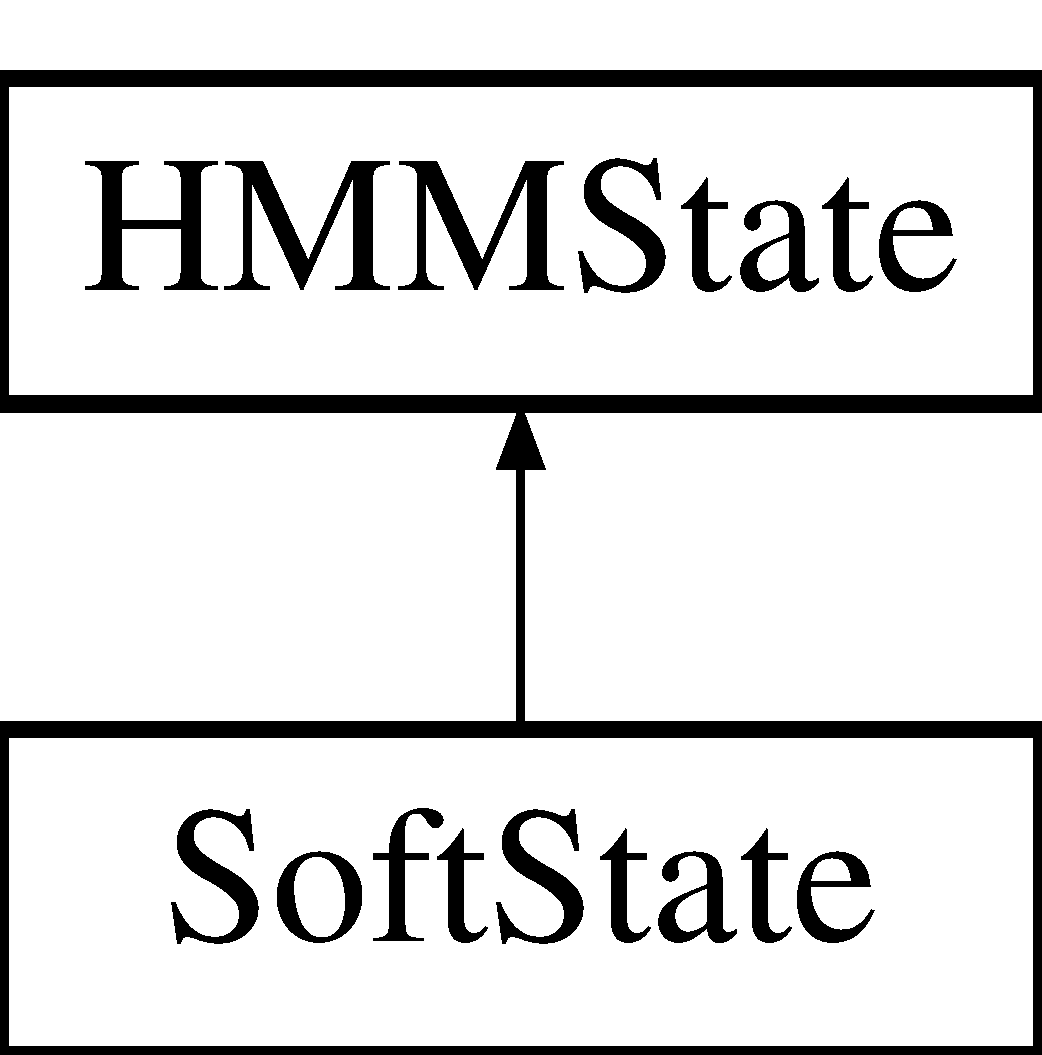
\includegraphics[height=2.000000cm]{class_soft_state}
\end{center}
\end{figure}
\subsection*{Public Member Functions}
\begin{DoxyCompactItemize}
\item 
\hyperlink{class_soft_state_a2e36cf999cc8ea73e00037093b4bd7cc}{Soft\+State} (std\+::vector$<$ \hyperlink{class_wave_feature_o_p}{Wave\+Feature\+O\+P} $>$ $\ast$\hyperlink{class_h_m_m_state_a04d0b1a1570a339e5cd0db13aeb0d2ae}{templates})
\item 
\hyperlink{class_soft_state_a99aeafbfb62ed73460d8f2d3d5011a5d}{$\sim$\+Soft\+State} ()
\item 
void \hyperlink{class_soft_state_ab7658b800fe20e84f8ed898d12c082a4}{gaussian\+Train} (int gaussian\+Num)
\item 
double \hyperlink{class_soft_state_aefe179676d2eb32304ddd04da60208f4}{node\+Cost} (\hyperlink{class_feature}{Feature} $\ast$input\+Feature)
\item 
void \hyperlink{class_soft_state_aa9666d6365a4f5fc0c329165f745c89e}{gaussian\+Train\+Test} (int gaussian\+Num)
\item 
double \hyperlink{class_soft_state_a37b85b634e49773fd85539cc2f55d62f}{node\+Cost\+Test} (\hyperlink{class_feature}{Feature} $\ast$input\+Feature)
\item 
void \hyperlink{class_soft_state_a157535fbd2cc224f30c06ac385a4377b}{load} (std\+::stringstream \&in, int \&\hyperlink{pro6__demo_8cpp_a923ffcfa3c56ccdba17bc4e700247d54}{gauss\+Num})
\item 
void \hyperlink{class_soft_state_a0d8a511a0ba9a18b797ecb07f96f944f}{store} (std\+::stringstream \&out)
\item 
void \hyperlink{class_soft_state_a5577579995771ff34512c576ddfd5885}{set\+Templates} (std\+::vector$<$ \hyperlink{class_wave_feature_o_p}{Wave\+Feature\+O\+P} $>$ $\ast$new\+Temps)
\item 
void \hyperlink{class_soft_state_a8945e17e64d61c11dedfd85d458c98e2}{dump} ()
\end{DoxyCompactItemize}
\subsection*{Private Member Functions}
\begin{DoxyCompactItemize}
\item 
void \hyperlink{class_soft_state_aefea07de56ed41dcc2045ab41ff537c3}{init\+Train} (int gaussian\+Num)
\item 
void \hyperlink{class_soft_state_aba68b421a253430d22d08af0ba4fc6a1}{Soft\+Train} ()
\item 
double \hyperlink{class_soft_state_a75dab3a7b75ba766e5861140778c582d}{Soft\+Node\+Cost} (\hyperlink{class_feature}{Feature} $\ast$\hyperlink{mel2hz_8m_a09113e60f6e326656763bae1603c0eb5}{f})
\item 
void \hyperlink{class_soft_state_ac2de89f2118ddacd321d98a0f1ffd027}{generate\+Init} (\hyperlink{class_feature}{Feature} \&feature)
\item 
void \hyperlink{class_soft_state_a4c673cabb4ae1a2550301f3130e1cf58}{clear\+Gaussian} ()
\item 
int \hyperlink{class_soft_state_a13bab7a425c6aad32270fb88bd81a026}{Point2\+Clusters} (int template\+Idx, int feature\+Idx)
\end{DoxyCompactItemize}
\subsection*{Private Attributes}
\begin{DoxyCompactItemize}
\item 
\hyperlink{configure__basic_8h_a566a006016cf65b1b01bd2bc633e1c12}{Matrix}$<$ double $>$ \hyperlink{class_soft_state_ac9dbfedcf51c0d3bf104d8d4b061f2ae}{probabilities}
\item 
std\+::vector$<$ \hyperlink{class_gaussian}{Gaussian} $\ast$ $>$ \hyperlink{class_soft_state_a5bb4abdc4477467c63accf9cb5699f55}{Gaussian\+Set}
\item 
std\+::vector$<$ double $>$ \hyperlink{class_soft_state_a7b4ebb0c683371ead7d0531acb7e0c5a}{weight}
\item 
double \hyperlink{class_soft_state_ace0f0548a8ece0e43299f7291c9155e2}{total\+Probability}
\item 
double \hyperlink{class_soft_state_a5172fb3fe754e9599b47fb738023d7cc}{max\+Probability}
\item 
double \hyperlink{class_soft_state_a7ac1e0c5327ce8dddd74bd649ed615e0}{u} \mbox{[}39\mbox{]}
\item 
double \hyperlink{class_soft_state_a329aa0dcdc7c6d628014e5ad86566c52}{sigma} \mbox{[}39\mbox{]}
\end{DoxyCompactItemize}
\subsection*{Friends}
\begin{DoxyCompactItemize}
\item 
class \hyperlink{class_soft_state_aa4adce0967898598e6f24f2024c247a3}{H\+M\+M\+Soft\+Automaton}
\item 
class \hyperlink{class_soft_state_a3f73063e67c75773ba856636249277b6}{H\+M\+M\+Automaton}
\end{DoxyCompactItemize}
\subsection*{Additional Inherited Members}


\subsection{Constructor \& Destructor Documentation}
\hypertarget{class_soft_state_a2e36cf999cc8ea73e00037093b4bd7cc}{\index{Soft\+State@{Soft\+State}!Soft\+State@{Soft\+State}}
\index{Soft\+State@{Soft\+State}!Soft\+State@{Soft\+State}}
\subsubsection[{Soft\+State}]{\setlength{\rightskip}{0pt plus 5cm}Soft\+State\+::\+Soft\+State (
\begin{DoxyParamCaption}
\item[{std\+::vector$<$ {\bf Wave\+Feature\+O\+P} $>$ $\ast$}]{templates}
\end{DoxyParamCaption}
)}}\label{class_soft_state_a2e36cf999cc8ea73e00037093b4bd7cc}
\hypertarget{class_soft_state_a99aeafbfb62ed73460d8f2d3d5011a5d}{\index{Soft\+State@{Soft\+State}!````~Soft\+State@{$\sim$\+Soft\+State}}
\index{````~Soft\+State@{$\sim$\+Soft\+State}!Soft\+State@{Soft\+State}}
\subsubsection[{$\sim$\+Soft\+State}]{\setlength{\rightskip}{0pt plus 5cm}Soft\+State\+::$\sim$\+Soft\+State (
\begin{DoxyParamCaption}
{}
\end{DoxyParamCaption}
)}}\label{class_soft_state_a99aeafbfb62ed73460d8f2d3d5011a5d}


\subsection{Member Function Documentation}
\hypertarget{class_soft_state_a4c673cabb4ae1a2550301f3130e1cf58}{\index{Soft\+State@{Soft\+State}!clear\+Gaussian@{clear\+Gaussian}}
\index{clear\+Gaussian@{clear\+Gaussian}!Soft\+State@{Soft\+State}}
\subsubsection[{clear\+Gaussian}]{\setlength{\rightskip}{0pt plus 5cm}void Soft\+State\+::clear\+Gaussian (
\begin{DoxyParamCaption}
{}
\end{DoxyParamCaption}
)\hspace{0.3cm}{\ttfamily [private]}}}\label{class_soft_state_a4c673cabb4ae1a2550301f3130e1cf58}
\hypertarget{class_soft_state_a8945e17e64d61c11dedfd85d458c98e2}{\index{Soft\+State@{Soft\+State}!dump@{dump}}
\index{dump@{dump}!Soft\+State@{Soft\+State}}
\subsubsection[{dump}]{\setlength{\rightskip}{0pt plus 5cm}void Soft\+State\+::dump (
\begin{DoxyParamCaption}
{}
\end{DoxyParamCaption}
)\hspace{0.3cm}{\ttfamily [inline]}}}\label{class_soft_state_a8945e17e64d61c11dedfd85d458c98e2}
\hypertarget{class_soft_state_ab7658b800fe20e84f8ed898d12c082a4}{\index{Soft\+State@{Soft\+State}!gaussian\+Train@{gaussian\+Train}}
\index{gaussian\+Train@{gaussian\+Train}!Soft\+State@{Soft\+State}}
\subsubsection[{gaussian\+Train}]{\setlength{\rightskip}{0pt plus 5cm}void Soft\+State\+::gaussian\+Train (
\begin{DoxyParamCaption}
\item[{int}]{gaussian\+Num}
\end{DoxyParamCaption}
)\hspace{0.3cm}{\ttfamily [virtual]}}}\label{class_soft_state_ab7658b800fe20e84f8ed898d12c082a4}


Implements \hyperlink{class_h_m_m_state_a2d42dd972a85014c0f5f9875da1eacd7}{H\+M\+M\+State}.

\hypertarget{class_soft_state_aa9666d6365a4f5fc0c329165f745c89e}{\index{Soft\+State@{Soft\+State}!gaussian\+Train\+Test@{gaussian\+Train\+Test}}
\index{gaussian\+Train\+Test@{gaussian\+Train\+Test}!Soft\+State@{Soft\+State}}
\subsubsection[{gaussian\+Train\+Test}]{\setlength{\rightskip}{0pt plus 5cm}void Soft\+State\+::gaussian\+Train\+Test (
\begin{DoxyParamCaption}
\item[{int}]{gaussian\+Num}
\end{DoxyParamCaption}
)}}\label{class_soft_state_aa9666d6365a4f5fc0c329165f745c89e}
\hypertarget{class_soft_state_ac2de89f2118ddacd321d98a0f1ffd027}{\index{Soft\+State@{Soft\+State}!generate\+Init@{generate\+Init}}
\index{generate\+Init@{generate\+Init}!Soft\+State@{Soft\+State}}
\subsubsection[{generate\+Init}]{\setlength{\rightskip}{0pt plus 5cm}void Soft\+State\+::generate\+Init (
\begin{DoxyParamCaption}
\item[{{\bf Feature} \&}]{feature}
\end{DoxyParamCaption}
)\hspace{0.3cm}{\ttfamily [private]}}}\label{class_soft_state_ac2de89f2118ddacd321d98a0f1ffd027}
\hypertarget{class_soft_state_aefea07de56ed41dcc2045ab41ff537c3}{\index{Soft\+State@{Soft\+State}!init\+Train@{init\+Train}}
\index{init\+Train@{init\+Train}!Soft\+State@{Soft\+State}}
\subsubsection[{init\+Train}]{\setlength{\rightskip}{0pt plus 5cm}void Soft\+State\+::init\+Train (
\begin{DoxyParamCaption}
\item[{int}]{gaussian\+Num}
\end{DoxyParamCaption}
)\hspace{0.3cm}{\ttfamily [private]}}}\label{class_soft_state_aefea07de56ed41dcc2045ab41ff537c3}
\hypertarget{class_soft_state_a157535fbd2cc224f30c06ac385a4377b}{\index{Soft\+State@{Soft\+State}!load@{load}}
\index{load@{load}!Soft\+State@{Soft\+State}}
\subsubsection[{load}]{\setlength{\rightskip}{0pt plus 5cm}void Soft\+State\+::load (
\begin{DoxyParamCaption}
\item[{std\+::stringstream \&}]{in, }
\item[{int \&}]{gauss\+Num}
\end{DoxyParamCaption}
)\hspace{0.3cm}{\ttfamily [virtual]}}}\label{class_soft_state_a157535fbd2cc224f30c06ac385a4377b}


Implements \hyperlink{class_h_m_m_state_ad5d14bf058b8fc39e07319fabebe09ee}{H\+M\+M\+State}.

\hypertarget{class_soft_state_aefe179676d2eb32304ddd04da60208f4}{\index{Soft\+State@{Soft\+State}!node\+Cost@{node\+Cost}}
\index{node\+Cost@{node\+Cost}!Soft\+State@{Soft\+State}}
\subsubsection[{node\+Cost}]{\setlength{\rightskip}{0pt plus 5cm}double Soft\+State\+::node\+Cost (
\begin{DoxyParamCaption}
\item[{{\bf Feature} $\ast$}]{input\+Feature}
\end{DoxyParamCaption}
)\hspace{0.3cm}{\ttfamily [virtual]}}}\label{class_soft_state_aefe179676d2eb32304ddd04da60208f4}


Implements \hyperlink{class_h_m_m_state_a84ad1899239f79257837e6d77cc4f242}{H\+M\+M\+State}.

\hypertarget{class_soft_state_a37b85b634e49773fd85539cc2f55d62f}{\index{Soft\+State@{Soft\+State}!node\+Cost\+Test@{node\+Cost\+Test}}
\index{node\+Cost\+Test@{node\+Cost\+Test}!Soft\+State@{Soft\+State}}
\subsubsection[{node\+Cost\+Test}]{\setlength{\rightskip}{0pt plus 5cm}double Soft\+State\+::node\+Cost\+Test (
\begin{DoxyParamCaption}
\item[{{\bf Feature} $\ast$}]{input\+Feature}
\end{DoxyParamCaption}
)}}\label{class_soft_state_a37b85b634e49773fd85539cc2f55d62f}
\hypertarget{class_soft_state_a13bab7a425c6aad32270fb88bd81a026}{\index{Soft\+State@{Soft\+State}!Point2\+Clusters@{Point2\+Clusters}}
\index{Point2\+Clusters@{Point2\+Clusters}!Soft\+State@{Soft\+State}}
\subsubsection[{Point2\+Clusters}]{\setlength{\rightskip}{0pt plus 5cm}int Soft\+State\+::\+Point2\+Clusters (
\begin{DoxyParamCaption}
\item[{int}]{template\+Idx, }
\item[{int}]{feature\+Idx}
\end{DoxyParamCaption}
)\hspace{0.3cm}{\ttfamily [private]}}}\label{class_soft_state_a13bab7a425c6aad32270fb88bd81a026}
\hypertarget{class_soft_state_a5577579995771ff34512c576ddfd5885}{\index{Soft\+State@{Soft\+State}!set\+Templates@{set\+Templates}}
\index{set\+Templates@{set\+Templates}!Soft\+State@{Soft\+State}}
\subsubsection[{set\+Templates}]{\setlength{\rightskip}{0pt plus 5cm}void Soft\+State\+::set\+Templates (
\begin{DoxyParamCaption}
\item[{std\+::vector$<$ {\bf Wave\+Feature\+O\+P} $>$ $\ast$}]{new\+Temps}
\end{DoxyParamCaption}
)\hspace{0.3cm}{\ttfamily [virtual]}}}\label{class_soft_state_a5577579995771ff34512c576ddfd5885}


Reimplemented from \hyperlink{class_h_m_m_state_ab9d6387b87e62ac03f4d15db1da7d7c7}{H\+M\+M\+State}.

\hypertarget{class_soft_state_a75dab3a7b75ba766e5861140778c582d}{\index{Soft\+State@{Soft\+State}!Soft\+Node\+Cost@{Soft\+Node\+Cost}}
\index{Soft\+Node\+Cost@{Soft\+Node\+Cost}!Soft\+State@{Soft\+State}}
\subsubsection[{Soft\+Node\+Cost}]{\setlength{\rightskip}{0pt plus 5cm}double Soft\+State\+::\+Soft\+Node\+Cost (
\begin{DoxyParamCaption}
\item[{{\bf Feature} $\ast$}]{f}
\end{DoxyParamCaption}
)\hspace{0.3cm}{\ttfamily [private]}}}\label{class_soft_state_a75dab3a7b75ba766e5861140778c582d}
\hypertarget{class_soft_state_aba68b421a253430d22d08af0ba4fc6a1}{\index{Soft\+State@{Soft\+State}!Soft\+Train@{Soft\+Train}}
\index{Soft\+Train@{Soft\+Train}!Soft\+State@{Soft\+State}}
\subsubsection[{Soft\+Train}]{\setlength{\rightskip}{0pt plus 5cm}void Soft\+State\+::\+Soft\+Train (
\begin{DoxyParamCaption}
{}
\end{DoxyParamCaption}
)\hspace{0.3cm}{\ttfamily [private]}}}\label{class_soft_state_aba68b421a253430d22d08af0ba4fc6a1}
\hypertarget{class_soft_state_a0d8a511a0ba9a18b797ecb07f96f944f}{\index{Soft\+State@{Soft\+State}!store@{store}}
\index{store@{store}!Soft\+State@{Soft\+State}}
\subsubsection[{store}]{\setlength{\rightskip}{0pt plus 5cm}void Soft\+State\+::store (
\begin{DoxyParamCaption}
\item[{std\+::stringstream \&}]{out}
\end{DoxyParamCaption}
)\hspace{0.3cm}{\ttfamily [virtual]}}}\label{class_soft_state_a0d8a511a0ba9a18b797ecb07f96f944f}


Implements \hyperlink{class_h_m_m_state_ab12116fc28ade677ee79ff13b4577ea6}{H\+M\+M\+State}.



\subsection{Friends And Related Function Documentation}
\hypertarget{class_soft_state_a3f73063e67c75773ba856636249277b6}{\index{Soft\+State@{Soft\+State}!H\+M\+M\+Automaton@{H\+M\+M\+Automaton}}
\index{H\+M\+M\+Automaton@{H\+M\+M\+Automaton}!Soft\+State@{Soft\+State}}
\subsubsection[{H\+M\+M\+Automaton}]{\setlength{\rightskip}{0pt plus 5cm}friend class {\bf H\+M\+M\+Automaton}\hspace{0.3cm}{\ttfamily [friend]}}}\label{class_soft_state_a3f73063e67c75773ba856636249277b6}
\hypertarget{class_soft_state_aa4adce0967898598e6f24f2024c247a3}{\index{Soft\+State@{Soft\+State}!H\+M\+M\+Soft\+Automaton@{H\+M\+M\+Soft\+Automaton}}
\index{H\+M\+M\+Soft\+Automaton@{H\+M\+M\+Soft\+Automaton}!Soft\+State@{Soft\+State}}
\subsubsection[{H\+M\+M\+Soft\+Automaton}]{\setlength{\rightskip}{0pt plus 5cm}friend class {\bf H\+M\+M\+Soft\+Automaton}\hspace{0.3cm}{\ttfamily [friend]}}}\label{class_soft_state_aa4adce0967898598e6f24f2024c247a3}


\subsection{Member Data Documentation}
\hypertarget{class_soft_state_a5bb4abdc4477467c63accf9cb5699f55}{\index{Soft\+State@{Soft\+State}!Gaussian\+Set@{Gaussian\+Set}}
\index{Gaussian\+Set@{Gaussian\+Set}!Soft\+State@{Soft\+State}}
\subsubsection[{Gaussian\+Set}]{\setlength{\rightskip}{0pt plus 5cm}std\+::vector$<${\bf Gaussian} $\ast$$>$ Soft\+State\+::\+Gaussian\+Set\hspace{0.3cm}{\ttfamily [private]}}}\label{class_soft_state_a5bb4abdc4477467c63accf9cb5699f55}
\hypertarget{class_soft_state_a5172fb3fe754e9599b47fb738023d7cc}{\index{Soft\+State@{Soft\+State}!max\+Probability@{max\+Probability}}
\index{max\+Probability@{max\+Probability}!Soft\+State@{Soft\+State}}
\subsubsection[{max\+Probability}]{\setlength{\rightskip}{0pt plus 5cm}double Soft\+State\+::max\+Probability\hspace{0.3cm}{\ttfamily [private]}}}\label{class_soft_state_a5172fb3fe754e9599b47fb738023d7cc}
\hypertarget{class_soft_state_ac9dbfedcf51c0d3bf104d8d4b061f2ae}{\index{Soft\+State@{Soft\+State}!probabilities@{probabilities}}
\index{probabilities@{probabilities}!Soft\+State@{Soft\+State}}
\subsubsection[{probabilities}]{\setlength{\rightskip}{0pt plus 5cm}{\bf Matrix}$<$double$>$ Soft\+State\+::probabilities\hspace{0.3cm}{\ttfamily [private]}}}\label{class_soft_state_ac9dbfedcf51c0d3bf104d8d4b061f2ae}
\hypertarget{class_soft_state_a329aa0dcdc7c6d628014e5ad86566c52}{\index{Soft\+State@{Soft\+State}!sigma@{sigma}}
\index{sigma@{sigma}!Soft\+State@{Soft\+State}}
\subsubsection[{sigma}]{\setlength{\rightskip}{0pt plus 5cm}double Soft\+State\+::sigma\mbox{[}39\mbox{]}\hspace{0.3cm}{\ttfamily [private]}}}\label{class_soft_state_a329aa0dcdc7c6d628014e5ad86566c52}
\hypertarget{class_soft_state_ace0f0548a8ece0e43299f7291c9155e2}{\index{Soft\+State@{Soft\+State}!total\+Probability@{total\+Probability}}
\index{total\+Probability@{total\+Probability}!Soft\+State@{Soft\+State}}
\subsubsection[{total\+Probability}]{\setlength{\rightskip}{0pt plus 5cm}double Soft\+State\+::total\+Probability\hspace{0.3cm}{\ttfamily [private]}}}\label{class_soft_state_ace0f0548a8ece0e43299f7291c9155e2}
\hypertarget{class_soft_state_a7ac1e0c5327ce8dddd74bd649ed615e0}{\index{Soft\+State@{Soft\+State}!u@{u}}
\index{u@{u}!Soft\+State@{Soft\+State}}
\subsubsection[{u}]{\setlength{\rightskip}{0pt plus 5cm}double Soft\+State\+::u\mbox{[}39\mbox{]}\hspace{0.3cm}{\ttfamily [private]}}}\label{class_soft_state_a7ac1e0c5327ce8dddd74bd649ed615e0}
\hypertarget{class_soft_state_a7b4ebb0c683371ead7d0531acb7e0c5a}{\index{Soft\+State@{Soft\+State}!weight@{weight}}
\index{weight@{weight}!Soft\+State@{Soft\+State}}
\subsubsection[{weight}]{\setlength{\rightskip}{0pt plus 5cm}std\+::vector$<$double$>$ Soft\+State\+::weight\hspace{0.3cm}{\ttfamily [private]}}}\label{class_soft_state_a7b4ebb0c683371ead7d0531acb7e0c5a}


The documentation for this class was generated from the following files\+:\begin{DoxyCompactItemize}
\item 
src/\+Feature/\hyperlink{_soft_state_8h}{Soft\+State.\+h}\item 
src/\+Feature/\hyperlink{_soft_state_8cpp}{Soft\+State.\+cpp}\end{DoxyCompactItemize}

\hypertarget{structsp__task}{\section{sp\+\_\+task Struct Reference}
\label{structsp__task}\index{sp\+\_\+task@{sp\+\_\+task}}
}


{\ttfamily \#include $<$Thread\+Pool.\+h$>$}

\subsection*{Public Attributes}
\begin{DoxyCompactItemize}
\item 
\hyperlink{_thread_pool_8h_a1eaa8749a99b9897592baf359529489b}{T\+A\+S\+K\+\_\+\+F\+U\+N\+C} \hyperlink{structsp__task_a6f57b2556c9756ba01dd48ed81241636}{func}
\item 
void $\ast$ \hyperlink{structsp__task_af558b254a2a1f6e80fd6060a0323f82a}{in}
\end{DoxyCompactItemize}


\subsection{Member Data Documentation}
\hypertarget{structsp__task_a6f57b2556c9756ba01dd48ed81241636}{\index{sp\+\_\+task@{sp\+\_\+task}!func@{func}}
\index{func@{func}!sp\+\_\+task@{sp\+\_\+task}}
\subsubsection[{func}]{\setlength{\rightskip}{0pt plus 5cm}{\bf T\+A\+S\+K\+\_\+\+F\+U\+N\+C} sp\+\_\+task\+::func}}\label{structsp__task_a6f57b2556c9756ba01dd48ed81241636}
\hypertarget{structsp__task_af558b254a2a1f6e80fd6060a0323f82a}{\index{sp\+\_\+task@{sp\+\_\+task}!in@{in}}
\index{in@{in}!sp\+\_\+task@{sp\+\_\+task}}
\subsubsection[{in}]{\setlength{\rightskip}{0pt plus 5cm}void$\ast$ sp\+\_\+task\+::in}}\label{structsp__task_af558b254a2a1f6e80fd6060a0323f82a}


The documentation for this struct was generated from the following file\+:\begin{DoxyCompactItemize}
\item 
src/\+Thread\+Pool/\hyperlink{_thread_pool_8h}{Thread\+Pool.\+h}\end{DoxyCompactItemize}

\hypertarget{class_spell_checker}{\section{Spell\+Checker Class Reference}
\label{class_spell_checker}\index{Spell\+Checker@{Spell\+Checker}}
}


{\ttfamily \#include $<$spellcheck.\+h$>$}

\subsection*{Public Member Functions}
\begin{DoxyCompactItemize}
\item 
\hyperlink{class_spell_checker_a900b34f6161abb0151678f34be07d8f9}{Spell\+Checker} (const char $\ast$dic\+File\+Name, int \hyperlink{class_spell_checker_acaf7176c06b86947773cbb83d7574783}{beam})
\item 
char $\ast$ \hyperlink{class_spell_checker_af5801d7b974e71ba7a382a5c5e056d41}{get\+Word} (int index)
\item 
void \hyperlink{class_spell_checker_aa7d8af30c6f029106004998b7d4da56d}{set\+Beam} (int b)
\item 
\hyperlink{class_spell_checker_ac65b662a48473a0b4c0b5b71e86c4b59}{Spell\+Checker} ()
\item 
\hyperlink{class_spell_checker_a26007dcd1c90cdaa790528e68443e9a6}{$\sim$\+Spell\+Checker} ()
\item 
int \hyperlink{class_spell_checker_a9b53c92d8e2ed48994d15c7ebdfa7176}{check} (const char $\ast$word, bool \hyperlink{class_spell_checker_a95d95e0ded8b4e1493a406746e509866}{one}=false, bool use\+\_\+path=true)
\item 
void \hyperlink{class_spell_checker_ad3f1f2d070dd63b772782d3d50605ac9}{show\+Info} ()
\item 
void \hyperlink{class_spell_checker_a187d460357c945d899977e0cd1269964}{print\+Ans} ()
\end{DoxyCompactItemize}
\subsection*{Public Attributes}
\begin{DoxyCompactItemize}
\item 
\hyperlink{class_link}{Link} \hyperlink{class_spell_checker_a935dea2584e5fdec80a2fe07e5cb08c3}{list} \mbox{[}2\mbox{]}
\end{DoxyCompactItemize}
\subsection*{Protected Member Functions}
\begin{DoxyCompactItemize}
\item 
\hyperlink{class_link}{Link} $\ast$ \hyperlink{class_spell_checker_aca55ad92aea6ede35932e868f6bbe66d}{init\+Link} ()
\item 
void \hyperlink{class_spell_checker_ae26f47f3595a3e4859172a4a1af87442}{refresh\+Link} (char next\+\_\+c, \hyperlink{class_link}{Link} \&now\+Link, \hyperlink{class_link}{Link} \&next\+Link, int)
\end{DoxyCompactItemize}
\subsection*{Protected Attributes}
\begin{DoxyCompactItemize}
\item 
int \hyperlink{class_spell_checker_acaf7176c06b86947773cbb83d7574783}{beam}
\end{DoxyCompactItemize}
\subsection*{Private Attributes}
\begin{DoxyCompactItemize}
\item 
bool \hyperlink{class_spell_checker_a95d95e0ded8b4e1493a406746e509866}{one}
\item 
\hyperlink{struct_path}{Path} \hyperlink{class_spell_checker_aff173fdb5d93d05cd3c130f8a5267272}{path}
\item 
\hyperlink{class_lex_tree}{Lex\+Tree} \hyperlink{class_spell_checker_abe9e58ca9de98d9a1182612a3c10a5aa}{tree}
\item 
int \hyperlink{class_spell_checker_a7c04bca12734e76005fe2535a3698ea5}{ansx}
\item 
int \hyperlink{class_spell_checker_aca76cb3fc436ef3970a100a950c4f11a}{ansy}
\end{DoxyCompactItemize}


\subsection{Constructor \& Destructor Documentation}
\hypertarget{class_spell_checker_a900b34f6161abb0151678f34be07d8f9}{\index{Spell\+Checker@{Spell\+Checker}!Spell\+Checker@{Spell\+Checker}}
\index{Spell\+Checker@{Spell\+Checker}!Spell\+Checker@{Spell\+Checker}}
\subsubsection[{Spell\+Checker}]{\setlength{\rightskip}{0pt plus 5cm}Spell\+Checker\+::\+Spell\+Checker (
\begin{DoxyParamCaption}
\item[{const char $\ast$}]{dic\+File\+Name, }
\item[{int}]{beam}
\end{DoxyParamCaption}
)\hspace{0.3cm}{\ttfamily [inline]}}}\label{class_spell_checker_a900b34f6161abb0151678f34be07d8f9}
\hypertarget{class_spell_checker_ac65b662a48473a0b4c0b5b71e86c4b59}{\index{Spell\+Checker@{Spell\+Checker}!Spell\+Checker@{Spell\+Checker}}
\index{Spell\+Checker@{Spell\+Checker}!Spell\+Checker@{Spell\+Checker}}
\subsubsection[{Spell\+Checker}]{\setlength{\rightskip}{0pt plus 5cm}Spell\+Checker\+::\+Spell\+Checker (
\begin{DoxyParamCaption}
{}
\end{DoxyParamCaption}
)}}\label{class_spell_checker_ac65b662a48473a0b4c0b5b71e86c4b59}
\hypertarget{class_spell_checker_a26007dcd1c90cdaa790528e68443e9a6}{\index{Spell\+Checker@{Spell\+Checker}!````~Spell\+Checker@{$\sim$\+Spell\+Checker}}
\index{````~Spell\+Checker@{$\sim$\+Spell\+Checker}!Spell\+Checker@{Spell\+Checker}}
\subsubsection[{$\sim$\+Spell\+Checker}]{\setlength{\rightskip}{0pt plus 5cm}Spell\+Checker\+::$\sim$\+Spell\+Checker (
\begin{DoxyParamCaption}
{}
\end{DoxyParamCaption}
)}}\label{class_spell_checker_a26007dcd1c90cdaa790528e68443e9a6}


\subsection{Member Function Documentation}
\hypertarget{class_spell_checker_a9b53c92d8e2ed48994d15c7ebdfa7176}{\index{Spell\+Checker@{Spell\+Checker}!check@{check}}
\index{check@{check}!Spell\+Checker@{Spell\+Checker}}
\subsubsection[{check}]{\setlength{\rightskip}{0pt plus 5cm}int Spell\+Checker\+::check (
\begin{DoxyParamCaption}
\item[{const char $\ast$}]{word, }
\item[{bool}]{one = {\ttfamily false}, }
\item[{bool}]{use\+\_\+path = {\ttfamily true}}
\end{DoxyParamCaption}
)}}\label{class_spell_checker_a9b53c92d8e2ed48994d15c7ebdfa7176}
!!! \hypertarget{class_spell_checker_af5801d7b974e71ba7a382a5c5e056d41}{\index{Spell\+Checker@{Spell\+Checker}!get\+Word@{get\+Word}}
\index{get\+Word@{get\+Word}!Spell\+Checker@{Spell\+Checker}}
\subsubsection[{get\+Word}]{\setlength{\rightskip}{0pt plus 5cm}char$\ast$ Spell\+Checker\+::get\+Word (
\begin{DoxyParamCaption}
\item[{int}]{index}
\end{DoxyParamCaption}
)\hspace{0.3cm}{\ttfamily [inline]}}}\label{class_spell_checker_af5801d7b974e71ba7a382a5c5e056d41}
\hypertarget{class_spell_checker_aca55ad92aea6ede35932e868f6bbe66d}{\index{Spell\+Checker@{Spell\+Checker}!init\+Link@{init\+Link}}
\index{init\+Link@{init\+Link}!Spell\+Checker@{Spell\+Checker}}
\subsubsection[{init\+Link}]{\setlength{\rightskip}{0pt plus 5cm}{\bf Link} $\ast$ Spell\+Checker\+::init\+Link (
\begin{DoxyParamCaption}
{}
\end{DoxyParamCaption}
)\hspace{0.3cm}{\ttfamily [protected]}}}\label{class_spell_checker_aca55ad92aea6ede35932e868f6bbe66d}
\hypertarget{class_spell_checker_a187d460357c945d899977e0cd1269964}{\index{Spell\+Checker@{Spell\+Checker}!print\+Ans@{print\+Ans}}
\index{print\+Ans@{print\+Ans}!Spell\+Checker@{Spell\+Checker}}
\subsubsection[{print\+Ans}]{\setlength{\rightskip}{0pt plus 5cm}void Spell\+Checker\+::print\+Ans (
\begin{DoxyParamCaption}
{}
\end{DoxyParamCaption}
)\hspace{0.3cm}{\ttfamily [inline]}}}\label{class_spell_checker_a187d460357c945d899977e0cd1269964}
\hypertarget{class_spell_checker_ae26f47f3595a3e4859172a4a1af87442}{\index{Spell\+Checker@{Spell\+Checker}!refresh\+Link@{refresh\+Link}}
\index{refresh\+Link@{refresh\+Link}!Spell\+Checker@{Spell\+Checker}}
\subsubsection[{refresh\+Link}]{\setlength{\rightskip}{0pt plus 5cm}void Spell\+Checker\+::refresh\+Link (
\begin{DoxyParamCaption}
\item[{char}]{next\+\_\+c, }
\item[{{\bf Link} \&}]{now\+Link, }
\item[{{\bf Link} \&}]{next\+Link, }
\item[{int}]{column}
\end{DoxyParamCaption}
)\hspace{0.3cm}{\ttfamily [protected]}}}\label{class_spell_checker_ae26f47f3595a3e4859172a4a1af87442}
\hypertarget{class_spell_checker_aa7d8af30c6f029106004998b7d4da56d}{\index{Spell\+Checker@{Spell\+Checker}!set\+Beam@{set\+Beam}}
\index{set\+Beam@{set\+Beam}!Spell\+Checker@{Spell\+Checker}}
\subsubsection[{set\+Beam}]{\setlength{\rightskip}{0pt plus 5cm}void Spell\+Checker\+::set\+Beam (
\begin{DoxyParamCaption}
\item[{int}]{b}
\end{DoxyParamCaption}
)\hspace{0.3cm}{\ttfamily [inline]}}}\label{class_spell_checker_aa7d8af30c6f029106004998b7d4da56d}
\hypertarget{class_spell_checker_ad3f1f2d070dd63b772782d3d50605ac9}{\index{Spell\+Checker@{Spell\+Checker}!show\+Info@{show\+Info}}
\index{show\+Info@{show\+Info}!Spell\+Checker@{Spell\+Checker}}
\subsubsection[{show\+Info}]{\setlength{\rightskip}{0pt plus 5cm}void Spell\+Checker\+::show\+Info (
\begin{DoxyParamCaption}
{}
\end{DoxyParamCaption}
)\hspace{0.3cm}{\ttfamily [inline]}}}\label{class_spell_checker_ad3f1f2d070dd63b772782d3d50605ac9}


\subsection{Member Data Documentation}
\hypertarget{class_spell_checker_a7c04bca12734e76005fe2535a3698ea5}{\index{Spell\+Checker@{Spell\+Checker}!ansx@{ansx}}
\index{ansx@{ansx}!Spell\+Checker@{Spell\+Checker}}
\subsubsection[{ansx}]{\setlength{\rightskip}{0pt plus 5cm}int Spell\+Checker\+::ansx\hspace{0.3cm}{\ttfamily [private]}}}\label{class_spell_checker_a7c04bca12734e76005fe2535a3698ea5}
\hypertarget{class_spell_checker_aca76cb3fc436ef3970a100a950c4f11a}{\index{Spell\+Checker@{Spell\+Checker}!ansy@{ansy}}
\index{ansy@{ansy}!Spell\+Checker@{Spell\+Checker}}
\subsubsection[{ansy}]{\setlength{\rightskip}{0pt plus 5cm}int Spell\+Checker\+::ansy\hspace{0.3cm}{\ttfamily [private]}}}\label{class_spell_checker_aca76cb3fc436ef3970a100a950c4f11a}
\hypertarget{class_spell_checker_acaf7176c06b86947773cbb83d7574783}{\index{Spell\+Checker@{Spell\+Checker}!beam@{beam}}
\index{beam@{beam}!Spell\+Checker@{Spell\+Checker}}
\subsubsection[{beam}]{\setlength{\rightskip}{0pt plus 5cm}int Spell\+Checker\+::beam\hspace{0.3cm}{\ttfamily [protected]}}}\label{class_spell_checker_acaf7176c06b86947773cbb83d7574783}
\hypertarget{class_spell_checker_a935dea2584e5fdec80a2fe07e5cb08c3}{\index{Spell\+Checker@{Spell\+Checker}!list@{list}}
\index{list@{list}!Spell\+Checker@{Spell\+Checker}}
\subsubsection[{list}]{\setlength{\rightskip}{0pt plus 5cm}{\bf Link} Spell\+Checker\+::list\mbox{[}2\mbox{]}}}\label{class_spell_checker_a935dea2584e5fdec80a2fe07e5cb08c3}
\hypertarget{class_spell_checker_a95d95e0ded8b4e1493a406746e509866}{\index{Spell\+Checker@{Spell\+Checker}!one@{one}}
\index{one@{one}!Spell\+Checker@{Spell\+Checker}}
\subsubsection[{one}]{\setlength{\rightskip}{0pt plus 5cm}bool Spell\+Checker\+::one\hspace{0.3cm}{\ttfamily [private]}}}\label{class_spell_checker_a95d95e0ded8b4e1493a406746e509866}
\hypertarget{class_spell_checker_aff173fdb5d93d05cd3c130f8a5267272}{\index{Spell\+Checker@{Spell\+Checker}!path@{path}}
\index{path@{path}!Spell\+Checker@{Spell\+Checker}}
\subsubsection[{path}]{\setlength{\rightskip}{0pt plus 5cm}{\bf Path} Spell\+Checker\+::path\hspace{0.3cm}{\ttfamily [private]}}}\label{class_spell_checker_aff173fdb5d93d05cd3c130f8a5267272}
\hypertarget{class_spell_checker_abe9e58ca9de98d9a1182612a3c10a5aa}{\index{Spell\+Checker@{Spell\+Checker}!tree@{tree}}
\index{tree@{tree}!Spell\+Checker@{Spell\+Checker}}
\subsubsection[{tree}]{\setlength{\rightskip}{0pt plus 5cm}{\bf Lex\+Tree} Spell\+Checker\+::tree\hspace{0.3cm}{\ttfamily [private]}}}\label{class_spell_checker_abe9e58ca9de98d9a1182612a3c10a5aa}


The documentation for this class was generated from the following files\+:\begin{DoxyCompactItemize}
\item 
src/\+Lex\+Tree/\hyperlink{spellcheck_8h}{spellcheck.\+h}\item 
src/\+Lex\+Tree/\hyperlink{spellcheck_8cpp}{spellcheck.\+cpp}\end{DoxyCompactItemize}

\hypertarget{structthread__info}{\section{thread\+\_\+info Struct Reference}
\label{structthread__info}\index{thread\+\_\+info@{thread\+\_\+info}}
}


{\ttfamily \#include $<$Thread\+Pool.\+h$>$}

\subsection*{Public Attributes}
\begin{DoxyCompactItemize}
\item 
std\+::vector$<$ \hyperlink{structsp__task}{sp\+\_\+task} $>$ \hyperlink{structthread__info_ab826b056145ce7f96e26908fa7de6398}{tasks}
\item 
pthread\+\_\+t \hyperlink{structthread__info_ae81f5cd44b9facefe8a6d35f872f5584}{tid}
\end{DoxyCompactItemize}


\subsection{Member Data Documentation}
\hypertarget{structthread__info_ab826b056145ce7f96e26908fa7de6398}{\index{thread\+\_\+info@{thread\+\_\+info}!tasks@{tasks}}
\index{tasks@{tasks}!thread\+\_\+info@{thread\+\_\+info}}
\subsubsection[{tasks}]{\setlength{\rightskip}{0pt plus 5cm}std\+::vector$<${\bf sp\+\_\+task}$>$ thread\+\_\+info\+::tasks}}\label{structthread__info_ab826b056145ce7f96e26908fa7de6398}
\hypertarget{structthread__info_ae81f5cd44b9facefe8a6d35f872f5584}{\index{thread\+\_\+info@{thread\+\_\+info}!tid@{tid}}
\index{tid@{tid}!thread\+\_\+info@{thread\+\_\+info}}
\subsubsection[{tid}]{\setlength{\rightskip}{0pt plus 5cm}pthread\+\_\+t thread\+\_\+info\+::tid}}\label{structthread__info_ae81f5cd44b9facefe8a6d35f872f5584}


The documentation for this struct was generated from the following file\+:\begin{DoxyCompactItemize}
\item 
src/\+Thread\+Pool/\hyperlink{_thread_pool_8h}{Thread\+Pool.\+h}\end{DoxyCompactItemize}

\hypertarget{class_thread_pool}{\section{Thread\+Pool Class Reference}
\label{class_thread_pool}\index{Thread\+Pool@{Thread\+Pool}}
}


{\ttfamily \#include $<$Thread\+Pool.\+h$>$}

\subsection*{Public Member Functions}
\begin{DoxyCompactItemize}
\item 
\hyperlink{class_thread_pool_a3225e86aa7835545b3f6c2c8d363d5e5}{Thread\+Pool} ()
\item 
\hyperlink{class_thread_pool_a2a6448ca556df8e8f9ab5242994dfb1e}{Thread\+Pool} (int \hyperlink{class_thread_pool_a080caea6c49348371e9ade20593da05d}{thread\+Num})
\item 
\hyperlink{class_thread_pool_a44d3d2ab618970605e684efc216655eb}{$\sim$\+Thread\+Pool} ()
\item 
void \hyperlink{class_thread_pool_af2281090fafb5b06e4cde7c7c1481525}{run} ()
\item 
void \hyperlink{class_thread_pool_a9e3e877fcf0f4ca4a146db6e139094f3}{add\+Task} (struct \hyperlink{structsp__task}{sp\+\_\+task} \&task)
\end{DoxyCompactItemize}
\subsection*{Static Public Attributes}
\begin{DoxyCompactItemize}
\item 
static int \hyperlink{class_thread_pool_a2bde4887496aa925585e188eb83cd2ee}{thread\+\_\+num} = \hyperlink{configure_8h_a42263ba14c8177f48c9eb58d6d912ad5}{D\+E\+F\+A\+U\+L\+T\+\_\+\+T\+H\+R\+E\+A\+D\+\_\+\+N\+U\+M}
\end{DoxyCompactItemize}
\subsection*{Private Member Functions}
\begin{DoxyCompactItemize}
\item 
void \hyperlink{class_thread_pool_a56b5e60a7b47491c8a74f87625b12695}{increament} ()
\end{DoxyCompactItemize}
\subsection*{Static Private Member Functions}
\begin{DoxyCompactItemize}
\item 
static void $\ast$ \hyperlink{class_thread_pool_a2c631f968dbc6527cdb49a612a528623}{process\+Thread} (void $\ast$)
\end{DoxyCompactItemize}
\subsection*{Private Attributes}
\begin{DoxyCompactItemize}
\item 
std\+::vector$<$ \hyperlink{structthread__info}{thread\+\_\+info} $>$ \hyperlink{class_thread_pool_acf827848f2f1da0a2e56309cc4359177}{thread\+Tasks}
\item 
int \hyperlink{class_thread_pool_a080caea6c49348371e9ade20593da05d}{thread\+Num}
\item 
int \hyperlink{class_thread_pool_a96d38c2d5e24c7ae9d01746ceafecb6b}{idx}
\end{DoxyCompactItemize}


\subsection{Constructor \& Destructor Documentation}
\hypertarget{class_thread_pool_a3225e86aa7835545b3f6c2c8d363d5e5}{\index{Thread\+Pool@{Thread\+Pool}!Thread\+Pool@{Thread\+Pool}}
\index{Thread\+Pool@{Thread\+Pool}!Thread\+Pool@{Thread\+Pool}}
\subsubsection[{Thread\+Pool}]{\setlength{\rightskip}{0pt plus 5cm}Thread\+Pool\+::\+Thread\+Pool (
\begin{DoxyParamCaption}
{}
\end{DoxyParamCaption}
)}}\label{class_thread_pool_a3225e86aa7835545b3f6c2c8d363d5e5}
\hypertarget{class_thread_pool_a2a6448ca556df8e8f9ab5242994dfb1e}{\index{Thread\+Pool@{Thread\+Pool}!Thread\+Pool@{Thread\+Pool}}
\index{Thread\+Pool@{Thread\+Pool}!Thread\+Pool@{Thread\+Pool}}
\subsubsection[{Thread\+Pool}]{\setlength{\rightskip}{0pt plus 5cm}Thread\+Pool\+::\+Thread\+Pool (
\begin{DoxyParamCaption}
\item[{int}]{thread\+Num}
\end{DoxyParamCaption}
)}}\label{class_thread_pool_a2a6448ca556df8e8f9ab5242994dfb1e}
\hypertarget{class_thread_pool_a44d3d2ab618970605e684efc216655eb}{\index{Thread\+Pool@{Thread\+Pool}!````~Thread\+Pool@{$\sim$\+Thread\+Pool}}
\index{````~Thread\+Pool@{$\sim$\+Thread\+Pool}!Thread\+Pool@{Thread\+Pool}}
\subsubsection[{$\sim$\+Thread\+Pool}]{\setlength{\rightskip}{0pt plus 5cm}Thread\+Pool\+::$\sim$\+Thread\+Pool (
\begin{DoxyParamCaption}
{}
\end{DoxyParamCaption}
)}}\label{class_thread_pool_a44d3d2ab618970605e684efc216655eb}


\subsection{Member Function Documentation}
\hypertarget{class_thread_pool_a9e3e877fcf0f4ca4a146db6e139094f3}{\index{Thread\+Pool@{Thread\+Pool}!add\+Task@{add\+Task}}
\index{add\+Task@{add\+Task}!Thread\+Pool@{Thread\+Pool}}
\subsubsection[{add\+Task}]{\setlength{\rightskip}{0pt plus 5cm}void Thread\+Pool\+::add\+Task (
\begin{DoxyParamCaption}
\item[{struct {\bf sp\+\_\+task} \&}]{task}
\end{DoxyParamCaption}
)}}\label{class_thread_pool_a9e3e877fcf0f4ca4a146db6e139094f3}
\hypertarget{class_thread_pool_a56b5e60a7b47491c8a74f87625b12695}{\index{Thread\+Pool@{Thread\+Pool}!increament@{increament}}
\index{increament@{increament}!Thread\+Pool@{Thread\+Pool}}
\subsubsection[{increament}]{\setlength{\rightskip}{0pt plus 5cm}void Thread\+Pool\+::increament (
\begin{DoxyParamCaption}
{}
\end{DoxyParamCaption}
)\hspace{0.3cm}{\ttfamily [inline]}, {\ttfamily [private]}}}\label{class_thread_pool_a56b5e60a7b47491c8a74f87625b12695}
\hypertarget{class_thread_pool_a2c631f968dbc6527cdb49a612a528623}{\index{Thread\+Pool@{Thread\+Pool}!process\+Thread@{process\+Thread}}
\index{process\+Thread@{process\+Thread}!Thread\+Pool@{Thread\+Pool}}
\subsubsection[{process\+Thread}]{\setlength{\rightskip}{0pt plus 5cm}void $\ast$ Thread\+Pool\+::process\+Thread (
\begin{DoxyParamCaption}
\item[{void $\ast$}]{param}
\end{DoxyParamCaption}
)\hspace{0.3cm}{\ttfamily [inline]}, {\ttfamily [static]}, {\ttfamily [private]}}}\label{class_thread_pool_a2c631f968dbc6527cdb49a612a528623}
\hypertarget{class_thread_pool_af2281090fafb5b06e4cde7c7c1481525}{\index{Thread\+Pool@{Thread\+Pool}!run@{run}}
\index{run@{run}!Thread\+Pool@{Thread\+Pool}}
\subsubsection[{run}]{\setlength{\rightskip}{0pt plus 5cm}void Thread\+Pool\+::run (
\begin{DoxyParamCaption}
{}
\end{DoxyParamCaption}
)}}\label{class_thread_pool_af2281090fafb5b06e4cde7c7c1481525}


\subsection{Member Data Documentation}
\hypertarget{class_thread_pool_a96d38c2d5e24c7ae9d01746ceafecb6b}{\index{Thread\+Pool@{Thread\+Pool}!idx@{idx}}
\index{idx@{idx}!Thread\+Pool@{Thread\+Pool}}
\subsubsection[{idx}]{\setlength{\rightskip}{0pt plus 5cm}int Thread\+Pool\+::idx\hspace{0.3cm}{\ttfamily [private]}}}\label{class_thread_pool_a96d38c2d5e24c7ae9d01746ceafecb6b}
\hypertarget{class_thread_pool_a2bde4887496aa925585e188eb83cd2ee}{\index{Thread\+Pool@{Thread\+Pool}!thread\+\_\+num@{thread\+\_\+num}}
\index{thread\+\_\+num@{thread\+\_\+num}!Thread\+Pool@{Thread\+Pool}}
\subsubsection[{thread\+\_\+num}]{\setlength{\rightskip}{0pt plus 5cm}int Thread\+Pool\+::thread\+\_\+num = {\bf D\+E\+F\+A\+U\+L\+T\+\_\+\+T\+H\+R\+E\+A\+D\+\_\+\+N\+U\+M}\hspace{0.3cm}{\ttfamily [static]}}}\label{class_thread_pool_a2bde4887496aa925585e188eb83cd2ee}
\hypertarget{class_thread_pool_a080caea6c49348371e9ade20593da05d}{\index{Thread\+Pool@{Thread\+Pool}!thread\+Num@{thread\+Num}}
\index{thread\+Num@{thread\+Num}!Thread\+Pool@{Thread\+Pool}}
\subsubsection[{thread\+Num}]{\setlength{\rightskip}{0pt plus 5cm}int Thread\+Pool\+::thread\+Num\hspace{0.3cm}{\ttfamily [private]}}}\label{class_thread_pool_a080caea6c49348371e9ade20593da05d}
\hypertarget{class_thread_pool_acf827848f2f1da0a2e56309cc4359177}{\index{Thread\+Pool@{Thread\+Pool}!thread\+Tasks@{thread\+Tasks}}
\index{thread\+Tasks@{thread\+Tasks}!Thread\+Pool@{Thread\+Pool}}
\subsubsection[{thread\+Tasks}]{\setlength{\rightskip}{0pt plus 5cm}std\+::vector$<$ {\bf thread\+\_\+info} $>$ Thread\+Pool\+::thread\+Tasks\hspace{0.3cm}{\ttfamily [private]}}}\label{class_thread_pool_acf827848f2f1da0a2e56309cc4359177}


The documentation for this class was generated from the following files\+:\begin{DoxyCompactItemize}
\item 
src/\+Thread\+Pool/\hyperlink{_thread_pool_8h}{Thread\+Pool.\+h}\item 
src/\+Thread\+Pool/\hyperlink{_thread_pool_8cpp}{Thread\+Pool.\+cpp}\end{DoxyCompactItemize}

\hypertarget{class_wave_feature_o_p}{\section{Wave\+Feature\+O\+P Class Reference}
\label{class_wave_feature_o_p}\index{Wave\+Feature\+O\+P@{Wave\+Feature\+O\+P}}
}


{\ttfamily \#include $<$Wave\+Feature\+O\+P.\+h$>$}

\subsection*{Public Types}
\begin{DoxyCompactItemize}
\item 
enum \hyperlink{class_wave_feature_o_p_a9c2fd724a37768ed03dc5b011d257500}{Op\+Type} \{ \hyperlink{class_wave_feature_o_p_a9c2fd724a37768ed03dc5b011d257500a60db933490e2134e59c4c2e1fb30ea66}{Raw}, 
\hyperlink{class_wave_feature_o_p_a9c2fd724a37768ed03dc5b011d257500a2aede4353c0fdb16edbc21db4085191e}{Beam}
 \}
\item 
enum \hyperlink{class_wave_feature_o_p_abd93c85d1ed5fbc148d41b7f32fc1d84}{L\+O\+A\+D\+\_\+\+T\+Y\+P\+E} \{ \hyperlink{class_wave_feature_o_p_abd93c85d1ed5fbc148d41b7f32fc1d84a56cb938408d6c1cfc350438fe83bb1a0}{O\+N\+L\+Y\+\_\+\+F\+I\+L\+E\+\_\+\+N\+A\+M\+E}, 
\hyperlink{class_wave_feature_o_p_abd93c85d1ed5fbc148d41b7f32fc1d84a1b64a07dfde0c2d4132bc343f4475856}{F\+U\+L\+L\+\_\+\+L\+O\+A\+D}
 \}
\end{DoxyCompactItemize}
\subsection*{Public Member Functions}
\begin{DoxyCompactItemize}
\item 
\hyperlink{class_wave_feature_o_p_a706b21be0839ad0693d98a39aa1be7f0}{Wave\+Feature\+O\+P} (const std\+::vector$<$ \hyperlink{class_feature}{Feature} $>$ \&template\+Feature, std\+::string file\+Name=\char`\"{}null\char`\"{}, std\+::string word=\char`\"{}null\char`\"{})
\item 
\hyperlink{class_wave_feature_o_p_ad046b3e250106abe16d9125a029bedc2}{$\sim$\+Wave\+Feature\+O\+P} ()
\item 
void \hyperlink{class_wave_feature_o_p_a39443a329cc706eaceefb28c598b297f}{syn\+Init} (std\+::vector$<$ \hyperlink{class_feature}{Feature} $>$ $\ast$\hyperlink{class_wave_feature_o_p_a2e67fe9dc06889453b70fe6efa19554f}{input\+Feature})
\item 
double \hyperlink{class_wave_feature_o_p_aa71ceac341c47742cb1ebe09bda1294a}{forward\+Column} (double \hyperlink{rawdtw_8cpp_afcfbedec6ebde62c6a091ce335836ef1}{threshold}=0.\+0)
\item 
double \hyperlink{class_wave_feature_o_p_a3a8dd15d19899586e5953886c7ee6de4}{asyn\+Dtw} (std\+::vector$<$ \hyperlink{class_feature}{Feature} $>$ $\ast$, double add\+Threshold=-\/5.\+0)
\item 
int \hyperlink{class_wave_feature_o_p_a44bed4fe2d42a232cd9f3e9d812ad240}{get\+Row\+Num} ()
\item 
\hyperlink{class_feature}{Feature} \& \hyperlink{class_wave_feature_o_p_a6a165bd04bb4f29e9b408981cca66328}{operator\mbox{[}$\,$\mbox{]}} (int idx)
\item 
int \hyperlink{class_wave_feature_o_p_a039099d115a4fa490ddb3296441a81e0}{size} ()
\item 
\hyperlink{tool_8h_ab71a1f2fb85a32402ced5c483105b38e}{S\+P\+\_\+\+R\+E\+S\+U\+L\+T} \hyperlink{class_wave_feature_o_p_aed6ce75f665daf168b5782672f89096a}{dump\+Color\+Path} (std\+::ostream \&Out)
\item 
bool \hyperlink{class_wave_feature_o_p_a124a8caab52ea00e1cf0165aa1d071c9}{operator==} (const \hyperlink{class_wave_feature_o_p}{Wave\+Feature\+O\+P} \&b)
\end{DoxyCompactItemize}
\subsection*{Private Member Functions}
\begin{DoxyCompactItemize}
\item 
\hyperlink{class_wave_feature_o_p_a2f106221542839a8cc7bf7289242ba73}{R\+E\+F\+E\+R\+E\+N\+C\+E\+\_\+\+R\+E\+A\+D\+\_\+\+O\+N\+L\+Y\+\_\+\+D\+E\+C\+L\+A\+R\+E} (std\+::vector$<$ \hyperlink{class_feature}{Feature} $>$, template\+Feature, Template\+Feature)
\item 
\hyperlink{class_wave_feature_o_p_a7fd393cae6541e5e5a4d341eca41e06f}{R\+E\+A\+D\+\_\+\+W\+R\+I\+T\+E\+\_\+\+D\+E\+C\+L\+A\+R\+E} (bool, do\+Record\+Path, Do\+Record\+Path)
\item 
\hyperlink{class_wave_feature_o_p_ab0a54a0e86eaa4a0c21f990f7280e6bd}{R\+E\+A\+D\+\_\+\+W\+R\+I\+T\+E\+\_\+\+D\+E\+C\+L\+A\+R\+E} (std\+::string, \hyperlink{rawdtw_8cpp_a7171b31127817befcc9fc0fb8f368a54}{template\+File\+Name}, File\+Name)
\item 
\hyperlink{class_wave_feature_o_p_a8c2271f6b26948fd6f4b8eb83ee72ed0}{R\+E\+A\+D\+\_\+\+W\+R\+I\+T\+E\+\_\+\+D\+E\+C\+L\+A\+R\+E} (std\+::string, \+\_\+word, Word)
\item 
\hyperlink{class_wave_feature_o_p_aa379ff8e29b7d67eb154ca1fd9b698f4}{R\+E\+A\+D\+\_\+\+W\+R\+I\+T\+E\+\_\+\+D\+E\+C\+L\+A\+R\+E} (\hyperlink{class_wave_feature_o_p_a9c2fd724a37768ed03dc5b011d257500}{Wave\+Feature\+O\+P\+::\+Op\+Type}, op\+Type, \hyperlink{class_wave_feature_o_p_a9c2fd724a37768ed03dc5b011d257500}{Op\+Type})
\item 
\hyperlink{class_wave_feature_o_p_a2851a010753b408b00e4077df2a8e1ce}{R\+E\+A\+D\+\_\+\+O\+N\+L\+Y\+\_\+\+D\+E\+C\+L\+A\+R\+E} (double, best\+Value, Dtw\+Result)
\item 
double \hyperlink{class_wave_feature_o_p_af586ac7dda241f1fd7def8a8a09a2181}{cal\+Dist} (int row\+Idx, int \hyperlink{class_wave_feature_o_p_a506bd025079326383412704dd93c402d}{column\+Idx})
\item 
void \hyperlink{class_wave_feature_o_p_a18142ce4be84ca4663c8ea8e208f5a02}{update\+Dtw\+Node} (int \hyperlink{class_wave_feature_o_p_a506bd025079326383412704dd93c402d}{column\+Idx}, int row\+Idx, double new\+Path\+Dist)
\item 
int \hyperlink{class_wave_feature_o_p_ac9c6eec84457d28e34b8002e364cecbc}{get\+Roll\+Idx} (int \hyperlink{class_wave_feature_o_p_a506bd025079326383412704dd93c402d}{column\+Idx})
\item 
void \hyperlink{class_wave_feature_o_p_a7568c3f771218b5e58988963a77e68da}{record\+Path} (int best\+Idx)
\end{DoxyCompactItemize}
\subsection*{Private Attributes}
\begin{DoxyCompactItemize}
\item 
std\+::vector$<$ int $>$ \hyperlink{class_wave_feature_o_p_a7e91a4de4afa4703c7e2e77e2ad6b73d}{path}
\item 
int \hyperlink{class_wave_feature_o_p_ad46053ff42554d848423b0caabeea87f}{head} \mbox{[}2\mbox{]}
\item 
std\+::vector$<$ int $>$ \hyperlink{class_wave_feature_o_p_ad14d7d2758bef1c990adda645f1a1d34}{column\+Nxt} \mbox{[}2\mbox{]}
\item 
std\+::vector$<$ double $>$ \hyperlink{class_wave_feature_o_p_a8341cc94705d4f96a53e61b397e26641}{column\+Dtw\+Res} \mbox{[}2\mbox{]}
\item 
std\+::vector$<$ int $>$ \hyperlink{class_wave_feature_o_p_abb3904a95a48013acf81a589a73983c0}{last\+Update}
\item 
std\+::vector$<$ \hyperlink{class_feature}{Feature} $>$ $\ast$ \hyperlink{class_wave_feature_o_p_a2e67fe9dc06889453b70fe6efa19554f}{input\+Feature}
\item 
int \hyperlink{class_wave_feature_o_p_a506bd025079326383412704dd93c402d}{column\+Idx}
\end{DoxyCompactItemize}
\subsection*{Static Private Attributes}
\begin{DoxyCompactItemize}
\item 
static const int \hyperlink{class_wave_feature_o_p_ad4482e96f3bca81925861baa598d01ed}{Path\+Split\+Idx} = -\/1
\end{DoxyCompactItemize}


\subsection{Member Enumeration Documentation}
\hypertarget{class_wave_feature_o_p_abd93c85d1ed5fbc148d41b7f32fc1d84}{\index{Wave\+Feature\+O\+P@{Wave\+Feature\+O\+P}!L\+O\+A\+D\+\_\+\+T\+Y\+P\+E@{L\+O\+A\+D\+\_\+\+T\+Y\+P\+E}}
\index{L\+O\+A\+D\+\_\+\+T\+Y\+P\+E@{L\+O\+A\+D\+\_\+\+T\+Y\+P\+E}!Wave\+Feature\+O\+P@{Wave\+Feature\+O\+P}}
\subsubsection[{L\+O\+A\+D\+\_\+\+T\+Y\+P\+E}]{\setlength{\rightskip}{0pt plus 5cm}enum {\bf Wave\+Feature\+O\+P\+::\+L\+O\+A\+D\+\_\+\+T\+Y\+P\+E}}}\label{class_wave_feature_o_p_abd93c85d1ed5fbc148d41b7f32fc1d84}
\begin{Desc}
\item[Enumerator]\par
\begin{description}
\index{O\+N\+L\+Y\+\_\+\+F\+I\+L\+E\+\_\+\+N\+A\+M\+E@{O\+N\+L\+Y\+\_\+\+F\+I\+L\+E\+\_\+\+N\+A\+M\+E}!Wave\+Feature\+O\+P@{Wave\+Feature\+O\+P}}\index{Wave\+Feature\+O\+P@{Wave\+Feature\+O\+P}!O\+N\+L\+Y\+\_\+\+F\+I\+L\+E\+\_\+\+N\+A\+M\+E@{O\+N\+L\+Y\+\_\+\+F\+I\+L\+E\+\_\+\+N\+A\+M\+E}}\item[{\em 
\hypertarget{class_wave_feature_o_p_abd93c85d1ed5fbc148d41b7f32fc1d84a56cb938408d6c1cfc350438fe83bb1a0}{O\+N\+L\+Y\+\_\+\+F\+I\+L\+E\+\_\+\+N\+A\+M\+E}\label{class_wave_feature_o_p_abd93c85d1ed5fbc148d41b7f32fc1d84a56cb938408d6c1cfc350438fe83bb1a0}
}]\index{F\+U\+L\+L\+\_\+\+L\+O\+A\+D@{F\+U\+L\+L\+\_\+\+L\+O\+A\+D}!Wave\+Feature\+O\+P@{Wave\+Feature\+O\+P}}\index{Wave\+Feature\+O\+P@{Wave\+Feature\+O\+P}!F\+U\+L\+L\+\_\+\+L\+O\+A\+D@{F\+U\+L\+L\+\_\+\+L\+O\+A\+D}}\item[{\em 
\hypertarget{class_wave_feature_o_p_abd93c85d1ed5fbc148d41b7f32fc1d84a1b64a07dfde0c2d4132bc343f4475856}{F\+U\+L\+L\+\_\+\+L\+O\+A\+D}\label{class_wave_feature_o_p_abd93c85d1ed5fbc148d41b7f32fc1d84a1b64a07dfde0c2d4132bc343f4475856}
}]\end{description}
\end{Desc}
\hypertarget{class_wave_feature_o_p_a9c2fd724a37768ed03dc5b011d257500}{\index{Wave\+Feature\+O\+P@{Wave\+Feature\+O\+P}!Op\+Type@{Op\+Type}}
\index{Op\+Type@{Op\+Type}!Wave\+Feature\+O\+P@{Wave\+Feature\+O\+P}}
\subsubsection[{Op\+Type}]{\setlength{\rightskip}{0pt plus 5cm}enum {\bf Wave\+Feature\+O\+P\+::\+Op\+Type}}}\label{class_wave_feature_o_p_a9c2fd724a37768ed03dc5b011d257500}
\begin{Desc}
\item[Enumerator]\par
\begin{description}
\index{Raw@{Raw}!Wave\+Feature\+O\+P@{Wave\+Feature\+O\+P}}\index{Wave\+Feature\+O\+P@{Wave\+Feature\+O\+P}!Raw@{Raw}}\item[{\em 
\hypertarget{class_wave_feature_o_p_a9c2fd724a37768ed03dc5b011d257500a60db933490e2134e59c4c2e1fb30ea66}{Raw}\label{class_wave_feature_o_p_a9c2fd724a37768ed03dc5b011d257500a60db933490e2134e59c4c2e1fb30ea66}
}]\index{Beam@{Beam}!Wave\+Feature\+O\+P@{Wave\+Feature\+O\+P}}\index{Wave\+Feature\+O\+P@{Wave\+Feature\+O\+P}!Beam@{Beam}}\item[{\em 
\hypertarget{class_wave_feature_o_p_a9c2fd724a37768ed03dc5b011d257500a2aede4353c0fdb16edbc21db4085191e}{Beam}\label{class_wave_feature_o_p_a9c2fd724a37768ed03dc5b011d257500a2aede4353c0fdb16edbc21db4085191e}
}]\end{description}
\end{Desc}


\subsection{Constructor \& Destructor Documentation}
\hypertarget{class_wave_feature_o_p_a706b21be0839ad0693d98a39aa1be7f0}{\index{Wave\+Feature\+O\+P@{Wave\+Feature\+O\+P}!Wave\+Feature\+O\+P@{Wave\+Feature\+O\+P}}
\index{Wave\+Feature\+O\+P@{Wave\+Feature\+O\+P}!Wave\+Feature\+O\+P@{Wave\+Feature\+O\+P}}
\subsubsection[{Wave\+Feature\+O\+P}]{\setlength{\rightskip}{0pt plus 5cm}Wave\+Feature\+O\+P\+::\+Wave\+Feature\+O\+P (
\begin{DoxyParamCaption}
\item[{const std\+::vector$<$ {\bf Feature} $>$ \&}]{template\+Feature, }
\item[{std\+::string}]{file\+Name = {\ttfamily \char`\"{}null\char`\"{}}, }
\item[{std\+::string}]{word = {\ttfamily \char`\"{}null\char`\"{}}}
\end{DoxyParamCaption}
)}}\label{class_wave_feature_o_p_a706b21be0839ad0693d98a39aa1be7f0}
\hypertarget{class_wave_feature_o_p_ad046b3e250106abe16d9125a029bedc2}{\index{Wave\+Feature\+O\+P@{Wave\+Feature\+O\+P}!````~Wave\+Feature\+O\+P@{$\sim$\+Wave\+Feature\+O\+P}}
\index{````~Wave\+Feature\+O\+P@{$\sim$\+Wave\+Feature\+O\+P}!Wave\+Feature\+O\+P@{Wave\+Feature\+O\+P}}
\subsubsection[{$\sim$\+Wave\+Feature\+O\+P}]{\setlength{\rightskip}{0pt plus 5cm}Wave\+Feature\+O\+P\+::$\sim$\+Wave\+Feature\+O\+P (
\begin{DoxyParamCaption}
{}
\end{DoxyParamCaption}
)\hspace{0.3cm}{\ttfamily [inline]}}}\label{class_wave_feature_o_p_ad046b3e250106abe16d9125a029bedc2}


\subsection{Member Function Documentation}
\hypertarget{class_wave_feature_o_p_a3a8dd15d19899586e5953886c7ee6de4}{\index{Wave\+Feature\+O\+P@{Wave\+Feature\+O\+P}!asyn\+Dtw@{asyn\+Dtw}}
\index{asyn\+Dtw@{asyn\+Dtw}!Wave\+Feature\+O\+P@{Wave\+Feature\+O\+P}}
\subsubsection[{asyn\+Dtw}]{\setlength{\rightskip}{0pt plus 5cm}double Wave\+Feature\+O\+P\+::asyn\+Dtw (
\begin{DoxyParamCaption}
\item[{std\+::vector$<$ {\bf Feature} $>$ $\ast$}]{input\+Feature, }
\item[{double}]{add\+Threshold = {\ttfamily -\/5.0}}
\end{DoxyParamCaption}
)}}\label{class_wave_feature_o_p_a3a8dd15d19899586e5953886c7ee6de4}
\hypertarget{class_wave_feature_o_p_af586ac7dda241f1fd7def8a8a09a2181}{\index{Wave\+Feature\+O\+P@{Wave\+Feature\+O\+P}!cal\+Dist@{cal\+Dist}}
\index{cal\+Dist@{cal\+Dist}!Wave\+Feature\+O\+P@{Wave\+Feature\+O\+P}}
\subsubsection[{cal\+Dist}]{\setlength{\rightskip}{0pt plus 5cm}double Wave\+Feature\+O\+P\+::cal\+Dist (
\begin{DoxyParamCaption}
\item[{int}]{row\+Idx, }
\item[{int}]{column\+Idx}
\end{DoxyParamCaption}
)\hspace{0.3cm}{\ttfamily [inline]}, {\ttfamily [private]}}}\label{class_wave_feature_o_p_af586ac7dda241f1fd7def8a8a09a2181}
\hypertarget{class_wave_feature_o_p_aed6ce75f665daf168b5782672f89096a}{\index{Wave\+Feature\+O\+P@{Wave\+Feature\+O\+P}!dump\+Color\+Path@{dump\+Color\+Path}}
\index{dump\+Color\+Path@{dump\+Color\+Path}!Wave\+Feature\+O\+P@{Wave\+Feature\+O\+P}}
\subsubsection[{dump\+Color\+Path}]{\setlength{\rightskip}{0pt plus 5cm}{\bf S\+P\+\_\+\+R\+E\+S\+U\+L\+T} Wave\+Feature\+O\+P\+::dump\+Color\+Path (
\begin{DoxyParamCaption}
\item[{std\+::ostream \&}]{Out}
\end{DoxyParamCaption}
)}}\label{class_wave_feature_o_p_aed6ce75f665daf168b5782672f89096a}
\hypertarget{class_wave_feature_o_p_aa71ceac341c47742cb1ebe09bda1294a}{\index{Wave\+Feature\+O\+P@{Wave\+Feature\+O\+P}!forward\+Column@{forward\+Column}}
\index{forward\+Column@{forward\+Column}!Wave\+Feature\+O\+P@{Wave\+Feature\+O\+P}}
\subsubsection[{forward\+Column}]{\setlength{\rightskip}{0pt plus 5cm}double Wave\+Feature\+O\+P\+::forward\+Column (
\begin{DoxyParamCaption}
\item[{double}]{threshold = {\ttfamily 0.0}}
\end{DoxyParamCaption}
)}}\label{class_wave_feature_o_p_aa71ceac341c47742cb1ebe09bda1294a}
\hypertarget{class_wave_feature_o_p_ac9c6eec84457d28e34b8002e364cecbc}{\index{Wave\+Feature\+O\+P@{Wave\+Feature\+O\+P}!get\+Roll\+Idx@{get\+Roll\+Idx}}
\index{get\+Roll\+Idx@{get\+Roll\+Idx}!Wave\+Feature\+O\+P@{Wave\+Feature\+O\+P}}
\subsubsection[{get\+Roll\+Idx}]{\setlength{\rightskip}{0pt plus 5cm}int Wave\+Feature\+O\+P\+::get\+Roll\+Idx (
\begin{DoxyParamCaption}
\item[{int}]{column\+Idx}
\end{DoxyParamCaption}
)\hspace{0.3cm}{\ttfamily [inline]}, {\ttfamily [private]}}}\label{class_wave_feature_o_p_ac9c6eec84457d28e34b8002e364cecbc}
\hypertarget{class_wave_feature_o_p_a44bed4fe2d42a232cd9f3e9d812ad240}{\index{Wave\+Feature\+O\+P@{Wave\+Feature\+O\+P}!get\+Row\+Num@{get\+Row\+Num}}
\index{get\+Row\+Num@{get\+Row\+Num}!Wave\+Feature\+O\+P@{Wave\+Feature\+O\+P}}
\subsubsection[{get\+Row\+Num}]{\setlength{\rightskip}{0pt plus 5cm}int Wave\+Feature\+O\+P\+::get\+Row\+Num (
\begin{DoxyParamCaption}
{}
\end{DoxyParamCaption}
)}}\label{class_wave_feature_o_p_a44bed4fe2d42a232cd9f3e9d812ad240}
\hypertarget{class_wave_feature_o_p_a124a8caab52ea00e1cf0165aa1d071c9}{\index{Wave\+Feature\+O\+P@{Wave\+Feature\+O\+P}!operator==@{operator==}}
\index{operator==@{operator==}!Wave\+Feature\+O\+P@{Wave\+Feature\+O\+P}}
\subsubsection[{operator==}]{\setlength{\rightskip}{0pt plus 5cm}bool Wave\+Feature\+O\+P\+::operator== (
\begin{DoxyParamCaption}
\item[{const {\bf Wave\+Feature\+O\+P} \&}]{b}
\end{DoxyParamCaption}
)}}\label{class_wave_feature_o_p_a124a8caab52ea00e1cf0165aa1d071c9}
\hypertarget{class_wave_feature_o_p_a6a165bd04bb4f29e9b408981cca66328}{\index{Wave\+Feature\+O\+P@{Wave\+Feature\+O\+P}!operator\mbox{[}$\,$\mbox{]}@{operator[]}}
\index{operator\mbox{[}$\,$\mbox{]}@{operator[]}!Wave\+Feature\+O\+P@{Wave\+Feature\+O\+P}}
\subsubsection[{operator[]}]{\setlength{\rightskip}{0pt plus 5cm}{\bf Feature} \& Wave\+Feature\+O\+P\+::operator\mbox{[}$\,$\mbox{]} (
\begin{DoxyParamCaption}
\item[{int}]{idx}
\end{DoxyParamCaption}
)}}\label{class_wave_feature_o_p_a6a165bd04bb4f29e9b408981cca66328}
\hypertarget{class_wave_feature_o_p_a2851a010753b408b00e4077df2a8e1ce}{\index{Wave\+Feature\+O\+P@{Wave\+Feature\+O\+P}!R\+E\+A\+D\+\_\+\+O\+N\+L\+Y\+\_\+\+D\+E\+C\+L\+A\+R\+E@{R\+E\+A\+D\+\_\+\+O\+N\+L\+Y\+\_\+\+D\+E\+C\+L\+A\+R\+E}}
\index{R\+E\+A\+D\+\_\+\+O\+N\+L\+Y\+\_\+\+D\+E\+C\+L\+A\+R\+E@{R\+E\+A\+D\+\_\+\+O\+N\+L\+Y\+\_\+\+D\+E\+C\+L\+A\+R\+E}!Wave\+Feature\+O\+P@{Wave\+Feature\+O\+P}}
\subsubsection[{R\+E\+A\+D\+\_\+\+O\+N\+L\+Y\+\_\+\+D\+E\+C\+L\+A\+R\+E}]{\setlength{\rightskip}{0pt plus 5cm}Wave\+Feature\+O\+P\+::\+R\+E\+A\+D\+\_\+\+O\+N\+L\+Y\+\_\+\+D\+E\+C\+L\+A\+R\+E (
\begin{DoxyParamCaption}
\item[{double}]{, }
\item[{best\+Value}]{, }
\item[{Dtw\+Result}]{}
\end{DoxyParamCaption}
)\hspace{0.3cm}{\ttfamily [private]}}}\label{class_wave_feature_o_p_a2851a010753b408b00e4077df2a8e1ce}
\hypertarget{class_wave_feature_o_p_a7fd393cae6541e5e5a4d341eca41e06f}{\index{Wave\+Feature\+O\+P@{Wave\+Feature\+O\+P}!R\+E\+A\+D\+\_\+\+W\+R\+I\+T\+E\+\_\+\+D\+E\+C\+L\+A\+R\+E@{R\+E\+A\+D\+\_\+\+W\+R\+I\+T\+E\+\_\+\+D\+E\+C\+L\+A\+R\+E}}
\index{R\+E\+A\+D\+\_\+\+W\+R\+I\+T\+E\+\_\+\+D\+E\+C\+L\+A\+R\+E@{R\+E\+A\+D\+\_\+\+W\+R\+I\+T\+E\+\_\+\+D\+E\+C\+L\+A\+R\+E}!Wave\+Feature\+O\+P@{Wave\+Feature\+O\+P}}
\subsubsection[{R\+E\+A\+D\+\_\+\+W\+R\+I\+T\+E\+\_\+\+D\+E\+C\+L\+A\+R\+E}]{\setlength{\rightskip}{0pt plus 5cm}Wave\+Feature\+O\+P\+::\+R\+E\+A\+D\+\_\+\+W\+R\+I\+T\+E\+\_\+\+D\+E\+C\+L\+A\+R\+E (
\begin{DoxyParamCaption}
\item[{bool}]{, }
\item[{do\+Record\+Path}]{, }
\item[{Do\+Record\+Path}]{}
\end{DoxyParamCaption}
)\hspace{0.3cm}{\ttfamily [private]}}}\label{class_wave_feature_o_p_a7fd393cae6541e5e5a4d341eca41e06f}
\hypertarget{class_wave_feature_o_p_ab0a54a0e86eaa4a0c21f990f7280e6bd}{\index{Wave\+Feature\+O\+P@{Wave\+Feature\+O\+P}!R\+E\+A\+D\+\_\+\+W\+R\+I\+T\+E\+\_\+\+D\+E\+C\+L\+A\+R\+E@{R\+E\+A\+D\+\_\+\+W\+R\+I\+T\+E\+\_\+\+D\+E\+C\+L\+A\+R\+E}}
\index{R\+E\+A\+D\+\_\+\+W\+R\+I\+T\+E\+\_\+\+D\+E\+C\+L\+A\+R\+E@{R\+E\+A\+D\+\_\+\+W\+R\+I\+T\+E\+\_\+\+D\+E\+C\+L\+A\+R\+E}!Wave\+Feature\+O\+P@{Wave\+Feature\+O\+P}}
\subsubsection[{R\+E\+A\+D\+\_\+\+W\+R\+I\+T\+E\+\_\+\+D\+E\+C\+L\+A\+R\+E}]{\setlength{\rightskip}{0pt plus 5cm}Wave\+Feature\+O\+P\+::\+R\+E\+A\+D\+\_\+\+W\+R\+I\+T\+E\+\_\+\+D\+E\+C\+L\+A\+R\+E (
\begin{DoxyParamCaption}
\item[{std\+::string}]{, }
\item[{{\bf template\+File\+Name}}]{, }
\item[{File\+Name}]{}
\end{DoxyParamCaption}
)\hspace{0.3cm}{\ttfamily [private]}}}\label{class_wave_feature_o_p_ab0a54a0e86eaa4a0c21f990f7280e6bd}
\hypertarget{class_wave_feature_o_p_a8c2271f6b26948fd6f4b8eb83ee72ed0}{\index{Wave\+Feature\+O\+P@{Wave\+Feature\+O\+P}!R\+E\+A\+D\+\_\+\+W\+R\+I\+T\+E\+\_\+\+D\+E\+C\+L\+A\+R\+E@{R\+E\+A\+D\+\_\+\+W\+R\+I\+T\+E\+\_\+\+D\+E\+C\+L\+A\+R\+E}}
\index{R\+E\+A\+D\+\_\+\+W\+R\+I\+T\+E\+\_\+\+D\+E\+C\+L\+A\+R\+E@{R\+E\+A\+D\+\_\+\+W\+R\+I\+T\+E\+\_\+\+D\+E\+C\+L\+A\+R\+E}!Wave\+Feature\+O\+P@{Wave\+Feature\+O\+P}}
\subsubsection[{R\+E\+A\+D\+\_\+\+W\+R\+I\+T\+E\+\_\+\+D\+E\+C\+L\+A\+R\+E}]{\setlength{\rightskip}{0pt plus 5cm}Wave\+Feature\+O\+P\+::\+R\+E\+A\+D\+\_\+\+W\+R\+I\+T\+E\+\_\+\+D\+E\+C\+L\+A\+R\+E (
\begin{DoxyParamCaption}
\item[{std\+::string}]{, }
\item[{\+\_\+word}]{, }
\item[{Word}]{}
\end{DoxyParamCaption}
)\hspace{0.3cm}{\ttfamily [private]}}}\label{class_wave_feature_o_p_a8c2271f6b26948fd6f4b8eb83ee72ed0}
\hypertarget{class_wave_feature_o_p_aa379ff8e29b7d67eb154ca1fd9b698f4}{\index{Wave\+Feature\+O\+P@{Wave\+Feature\+O\+P}!R\+E\+A\+D\+\_\+\+W\+R\+I\+T\+E\+\_\+\+D\+E\+C\+L\+A\+R\+E@{R\+E\+A\+D\+\_\+\+W\+R\+I\+T\+E\+\_\+\+D\+E\+C\+L\+A\+R\+E}}
\index{R\+E\+A\+D\+\_\+\+W\+R\+I\+T\+E\+\_\+\+D\+E\+C\+L\+A\+R\+E@{R\+E\+A\+D\+\_\+\+W\+R\+I\+T\+E\+\_\+\+D\+E\+C\+L\+A\+R\+E}!Wave\+Feature\+O\+P@{Wave\+Feature\+O\+P}}
\subsubsection[{R\+E\+A\+D\+\_\+\+W\+R\+I\+T\+E\+\_\+\+D\+E\+C\+L\+A\+R\+E}]{\setlength{\rightskip}{0pt plus 5cm}Wave\+Feature\+O\+P\+::\+R\+E\+A\+D\+\_\+\+W\+R\+I\+T\+E\+\_\+\+D\+E\+C\+L\+A\+R\+E (
\begin{DoxyParamCaption}
\item[{{\bf Wave\+Feature\+O\+P\+::\+Op\+Type}}]{, }
\item[{op\+Type}]{, }
\item[{{\bf Op\+Type}}]{}
\end{DoxyParamCaption}
)\hspace{0.3cm}{\ttfamily [private]}}}\label{class_wave_feature_o_p_aa379ff8e29b7d67eb154ca1fd9b698f4}
\hypertarget{class_wave_feature_o_p_a7568c3f771218b5e58988963a77e68da}{\index{Wave\+Feature\+O\+P@{Wave\+Feature\+O\+P}!record\+Path@{record\+Path}}
\index{record\+Path@{record\+Path}!Wave\+Feature\+O\+P@{Wave\+Feature\+O\+P}}
\subsubsection[{record\+Path}]{\setlength{\rightskip}{0pt plus 5cm}void Wave\+Feature\+O\+P\+::record\+Path (
\begin{DoxyParamCaption}
\item[{int}]{best\+Idx}
\end{DoxyParamCaption}
)\hspace{0.3cm}{\ttfamily [inline]}, {\ttfamily [private]}}}\label{class_wave_feature_o_p_a7568c3f771218b5e58988963a77e68da}
\hypertarget{class_wave_feature_o_p_a2f106221542839a8cc7bf7289242ba73}{\index{Wave\+Feature\+O\+P@{Wave\+Feature\+O\+P}!R\+E\+F\+E\+R\+E\+N\+C\+E\+\_\+\+R\+E\+A\+D\+\_\+\+O\+N\+L\+Y\+\_\+\+D\+E\+C\+L\+A\+R\+E@{R\+E\+F\+E\+R\+E\+N\+C\+E\+\_\+\+R\+E\+A\+D\+\_\+\+O\+N\+L\+Y\+\_\+\+D\+E\+C\+L\+A\+R\+E}}
\index{R\+E\+F\+E\+R\+E\+N\+C\+E\+\_\+\+R\+E\+A\+D\+\_\+\+O\+N\+L\+Y\+\_\+\+D\+E\+C\+L\+A\+R\+E@{R\+E\+F\+E\+R\+E\+N\+C\+E\+\_\+\+R\+E\+A\+D\+\_\+\+O\+N\+L\+Y\+\_\+\+D\+E\+C\+L\+A\+R\+E}!Wave\+Feature\+O\+P@{Wave\+Feature\+O\+P}}
\subsubsection[{R\+E\+F\+E\+R\+E\+N\+C\+E\+\_\+\+R\+E\+A\+D\+\_\+\+O\+N\+L\+Y\+\_\+\+D\+E\+C\+L\+A\+R\+E}]{\setlength{\rightskip}{0pt plus 5cm}Wave\+Feature\+O\+P\+::\+R\+E\+F\+E\+R\+E\+N\+C\+E\+\_\+\+R\+E\+A\+D\+\_\+\+O\+N\+L\+Y\+\_\+\+D\+E\+C\+L\+A\+R\+E (
\begin{DoxyParamCaption}
\item[{std\+::vector$<$ {\bf Feature} $>$}]{, }
\item[{template\+Feature}]{, }
\item[{Template\+Feature}]{}
\end{DoxyParamCaption}
)\hspace{0.3cm}{\ttfamily [private]}}}\label{class_wave_feature_o_p_a2f106221542839a8cc7bf7289242ba73}
\hypertarget{class_wave_feature_o_p_a039099d115a4fa490ddb3296441a81e0}{\index{Wave\+Feature\+O\+P@{Wave\+Feature\+O\+P}!size@{size}}
\index{size@{size}!Wave\+Feature\+O\+P@{Wave\+Feature\+O\+P}}
\subsubsection[{size}]{\setlength{\rightskip}{0pt plus 5cm}int Wave\+Feature\+O\+P\+::size (
\begin{DoxyParamCaption}
{}
\end{DoxyParamCaption}
)}}\label{class_wave_feature_o_p_a039099d115a4fa490ddb3296441a81e0}
\hypertarget{class_wave_feature_o_p_a39443a329cc706eaceefb28c598b297f}{\index{Wave\+Feature\+O\+P@{Wave\+Feature\+O\+P}!syn\+Init@{syn\+Init}}
\index{syn\+Init@{syn\+Init}!Wave\+Feature\+O\+P@{Wave\+Feature\+O\+P}}
\subsubsection[{syn\+Init}]{\setlength{\rightskip}{0pt plus 5cm}void Wave\+Feature\+O\+P\+::syn\+Init (
\begin{DoxyParamCaption}
\item[{std\+::vector$<$ {\bf Feature} $>$ $\ast$}]{input\+Feature}
\end{DoxyParamCaption}
)}}\label{class_wave_feature_o_p_a39443a329cc706eaceefb28c598b297f}
\hypertarget{class_wave_feature_o_p_a18142ce4be84ca4663c8ea8e208f5a02}{\index{Wave\+Feature\+O\+P@{Wave\+Feature\+O\+P}!update\+Dtw\+Node@{update\+Dtw\+Node}}
\index{update\+Dtw\+Node@{update\+Dtw\+Node}!Wave\+Feature\+O\+P@{Wave\+Feature\+O\+P}}
\subsubsection[{update\+Dtw\+Node}]{\setlength{\rightskip}{0pt plus 5cm}void Wave\+Feature\+O\+P\+::update\+Dtw\+Node (
\begin{DoxyParamCaption}
\item[{int}]{column\+Idx, }
\item[{int}]{row\+Idx, }
\item[{double}]{new\+Path\+Dist}
\end{DoxyParamCaption}
)\hspace{0.3cm}{\ttfamily [inline]}, {\ttfamily [private]}}}\label{class_wave_feature_o_p_a18142ce4be84ca4663c8ea8e208f5a02}


\subsection{Member Data Documentation}
\hypertarget{class_wave_feature_o_p_a8341cc94705d4f96a53e61b397e26641}{\index{Wave\+Feature\+O\+P@{Wave\+Feature\+O\+P}!column\+Dtw\+Res@{column\+Dtw\+Res}}
\index{column\+Dtw\+Res@{column\+Dtw\+Res}!Wave\+Feature\+O\+P@{Wave\+Feature\+O\+P}}
\subsubsection[{column\+Dtw\+Res}]{\setlength{\rightskip}{0pt plus 5cm}std\+::vector$<$double$>$ Wave\+Feature\+O\+P\+::column\+Dtw\+Res\mbox{[}2\mbox{]}\hspace{0.3cm}{\ttfamily [private]}}}\label{class_wave_feature_o_p_a8341cc94705d4f96a53e61b397e26641}
\hypertarget{class_wave_feature_o_p_a506bd025079326383412704dd93c402d}{\index{Wave\+Feature\+O\+P@{Wave\+Feature\+O\+P}!column\+Idx@{column\+Idx}}
\index{column\+Idx@{column\+Idx}!Wave\+Feature\+O\+P@{Wave\+Feature\+O\+P}}
\subsubsection[{column\+Idx}]{\setlength{\rightskip}{0pt plus 5cm}int Wave\+Feature\+O\+P\+::column\+Idx\hspace{0.3cm}{\ttfamily [private]}}}\label{class_wave_feature_o_p_a506bd025079326383412704dd93c402d}
\hypertarget{class_wave_feature_o_p_ad14d7d2758bef1c990adda645f1a1d34}{\index{Wave\+Feature\+O\+P@{Wave\+Feature\+O\+P}!column\+Nxt@{column\+Nxt}}
\index{column\+Nxt@{column\+Nxt}!Wave\+Feature\+O\+P@{Wave\+Feature\+O\+P}}
\subsubsection[{column\+Nxt}]{\setlength{\rightskip}{0pt plus 5cm}std\+::vector$<$int$>$ Wave\+Feature\+O\+P\+::column\+Nxt\mbox{[}2\mbox{]}\hspace{0.3cm}{\ttfamily [private]}}}\label{class_wave_feature_o_p_ad14d7d2758bef1c990adda645f1a1d34}
\hypertarget{class_wave_feature_o_p_ad46053ff42554d848423b0caabeea87f}{\index{Wave\+Feature\+O\+P@{Wave\+Feature\+O\+P}!head@{head}}
\index{head@{head}!Wave\+Feature\+O\+P@{Wave\+Feature\+O\+P}}
\subsubsection[{head}]{\setlength{\rightskip}{0pt plus 5cm}int Wave\+Feature\+O\+P\+::head\mbox{[}2\mbox{]}\hspace{0.3cm}{\ttfamily [private]}}}\label{class_wave_feature_o_p_ad46053ff42554d848423b0caabeea87f}
\hypertarget{class_wave_feature_o_p_a2e67fe9dc06889453b70fe6efa19554f}{\index{Wave\+Feature\+O\+P@{Wave\+Feature\+O\+P}!input\+Feature@{input\+Feature}}
\index{input\+Feature@{input\+Feature}!Wave\+Feature\+O\+P@{Wave\+Feature\+O\+P}}
\subsubsection[{input\+Feature}]{\setlength{\rightskip}{0pt plus 5cm}std\+::vector$<${\bf Feature}$>$$\ast$ Wave\+Feature\+O\+P\+::input\+Feature\hspace{0.3cm}{\ttfamily [private]}}}\label{class_wave_feature_o_p_a2e67fe9dc06889453b70fe6efa19554f}
\hypertarget{class_wave_feature_o_p_abb3904a95a48013acf81a589a73983c0}{\index{Wave\+Feature\+O\+P@{Wave\+Feature\+O\+P}!last\+Update@{last\+Update}}
\index{last\+Update@{last\+Update}!Wave\+Feature\+O\+P@{Wave\+Feature\+O\+P}}
\subsubsection[{last\+Update}]{\setlength{\rightskip}{0pt plus 5cm}std\+::vector$<$int$>$ Wave\+Feature\+O\+P\+::last\+Update\hspace{0.3cm}{\ttfamily [private]}}}\label{class_wave_feature_o_p_abb3904a95a48013acf81a589a73983c0}
\hypertarget{class_wave_feature_o_p_a7e91a4de4afa4703c7e2e77e2ad6b73d}{\index{Wave\+Feature\+O\+P@{Wave\+Feature\+O\+P}!path@{path}}
\index{path@{path}!Wave\+Feature\+O\+P@{Wave\+Feature\+O\+P}}
\subsubsection[{path}]{\setlength{\rightskip}{0pt plus 5cm}std\+::vector$<$int$>$ Wave\+Feature\+O\+P\+::path\hspace{0.3cm}{\ttfamily [private]}}}\label{class_wave_feature_o_p_a7e91a4de4afa4703c7e2e77e2ad6b73d}
\hypertarget{class_wave_feature_o_p_ad4482e96f3bca81925861baa598d01ed}{\index{Wave\+Feature\+O\+P@{Wave\+Feature\+O\+P}!Path\+Split\+Idx@{Path\+Split\+Idx}}
\index{Path\+Split\+Idx@{Path\+Split\+Idx}!Wave\+Feature\+O\+P@{Wave\+Feature\+O\+P}}
\subsubsection[{Path\+Split\+Idx}]{\setlength{\rightskip}{0pt plus 5cm}const int Wave\+Feature\+O\+P\+::\+Path\+Split\+Idx = -\/1\hspace{0.3cm}{\ttfamily [static]}, {\ttfamily [private]}}}\label{class_wave_feature_o_p_ad4482e96f3bca81925861baa598d01ed}


The documentation for this class was generated from the following files\+:\begin{DoxyCompactItemize}
\item 
src/\+Feature/\hyperlink{_wave_feature_o_p_8h}{Wave\+Feature\+O\+P.\+h}\item 
src/\+Feature/\hyperlink{_wave_feature_o_p_8cpp}{Wave\+Feature\+O\+P.\+cpp}\end{DoxyCompactItemize}

\hypertarget{class_wave_feature_o_p_set}{\section{Wave\+Feature\+O\+P\+Set Class Reference}
\label{class_wave_feature_o_p_set}\index{Wave\+Feature\+O\+P\+Set@{Wave\+Feature\+O\+P\+Set}}
}


{\ttfamily \#include $<$Wave\+Feature\+O\+P\+Set.\+h$>$}

Inheritance diagram for Wave\+Feature\+O\+P\+Set\+:\begin{figure}[H]
\begin{center}
\leavevmode
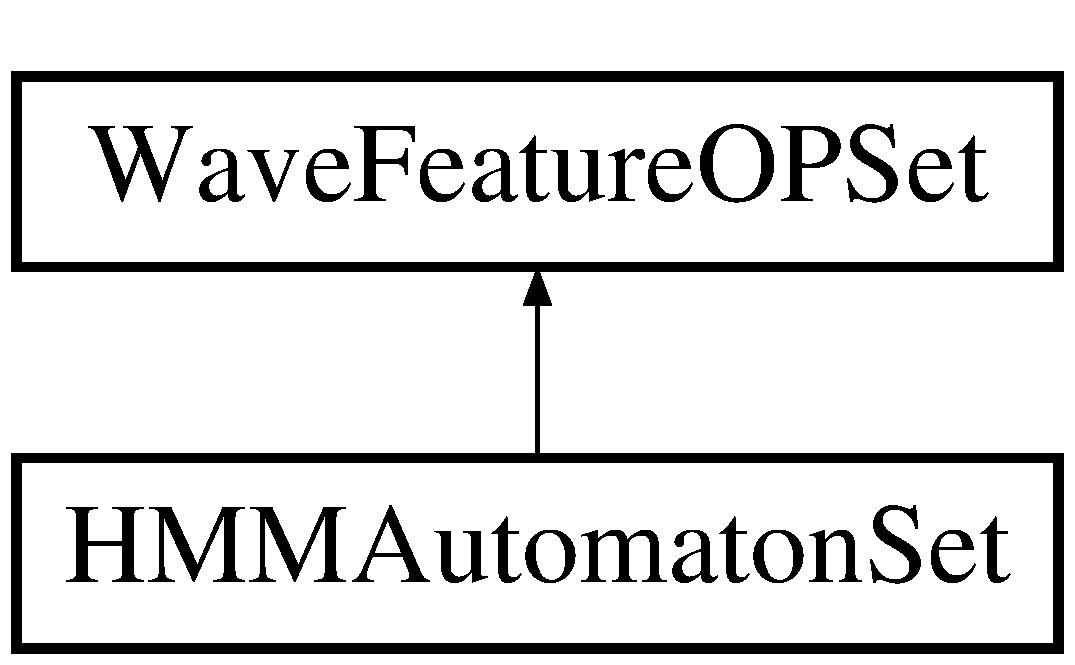
\includegraphics[height=2.000000cm]{class_wave_feature_o_p_set}
\end{center}
\end{figure}
\subsection*{Classes}
\begin{DoxyCompactItemize}
\item 
class \hyperlink{class_wave_feature_o_p_set_1_1iterator}{iterator}
\end{DoxyCompactItemize}
\subsection*{Public Types}
\begin{DoxyCompactItemize}
\item 
typedef std\+::map$<$ std\+::string, \\*
std\+::vector$<$ \hyperlink{class_wave_feature_o_p}{Wave\+Feature\+O\+P} $>$ $>$ \hyperlink{class_wave_feature_o_p_set_a7145e9463a1fb85ce4c239552bf4e8e0}{data\+Set\+Type}
\end{DoxyCompactItemize}
\subsection*{Public Member Functions}
\begin{DoxyCompactItemize}
\item 
\hyperlink{class_wave_feature_o_p_set_1_1iterator}{iterator} \hyperlink{class_wave_feature_o_p_set_ac5aad41310f38626a922ec74920b7a0e}{begin} ()
\item 
\hyperlink{class_wave_feature_o_p_set_1_1iterator}{iterator} \hyperlink{class_wave_feature_o_p_set_a7df62d3222f8896143b8a0c336ccbb18}{end} ()
\item 
virtual \hyperlink{tool_8h_ab71a1f2fb85a32402ced5c483105b38e}{S\+P\+\_\+\+R\+E\+S\+U\+L\+T} \hyperlink{class_wave_feature_o_p_set_ac0643637484df06ccf4336a48cd4f765}{load\+Mfccs} (char $\ast$template\+Dir, \hyperlink{class_wave_feature_o_p_abd93c85d1ed5fbc148d41b7f32fc1d84}{Wave\+Feature\+O\+P\+::\+L\+O\+A\+D\+\_\+\+T\+Y\+P\+E} load\+Type=\hyperlink{class_wave_feature_o_p_abd93c85d1ed5fbc148d41b7f32fc1d84a1b64a07dfde0c2d4132bc343f4475856}{Wave\+Feature\+O\+P\+::\+F\+U\+L\+L\+\_\+\+L\+O\+A\+D})
\item 
virtual \hyperlink{tool_8h_ab71a1f2fb85a32402ced5c483105b38e}{S\+P\+\_\+\+R\+E\+S\+U\+L\+T} \hyperlink{class_wave_feature_o_p_set_ab1bc5a7acaba431993da7d784390bd83}{load\+Mfccs} (char $\ast$template\+Dir, char $\ast$file\+Name, \hyperlink{class_wave_feature_o_p_abd93c85d1ed5fbc148d41b7f32fc1d84}{Wave\+Feature\+O\+P\+::\+L\+O\+A\+D\+\_\+\+T\+Y\+P\+E} load\+Type=\hyperlink{class_wave_feature_o_p_abd93c85d1ed5fbc148d41b7f32fc1d84a1b64a07dfde0c2d4132bc343f4475856}{Wave\+Feature\+O\+P\+::\+F\+U\+L\+L\+\_\+\+L\+O\+A\+D})
\item 
\hyperlink{class_wave_feature_o_p_set_abc2105d69e5f9b1cad09b83de86a4d00}{Wave\+Feature\+O\+P\+Set} (int \hyperlink{pro4__demo__1_8cpp_adc01d2f6980a1af5c3ddc83d847dafa0}{max\+Instance\+Per}=\hyperlink{configure__dtw_8h_a5e1cc8ac4ebc0912817c618ccc9d823b}{M\+A\+X\+\_\+\+T\+E\+M\+P\+L\+A\+T\+E\+S\+\_\+\+P\+E\+R\+\_\+\+W\+O\+R\+D})
\item 
virtual \hyperlink{class_wave_feature_o_p_set_acbc8ed8d5dcf2624dcc1a985baa63c8e}{$\sim$\+Wave\+Feature\+O\+P\+Set} ()
\end{DoxyCompactItemize}
\subsection*{Protected Attributes}
\begin{DoxyCompactItemize}
\item 
\hyperlink{class_wave_feature_o_p_set_a7145e9463a1fb85ce4c239552bf4e8e0}{data\+Set\+Type} \hyperlink{class_wave_feature_o_p_set_ab536eab1f12dec8e95c4459f6cbcd3f1}{data\+Set}
\end{DoxyCompactItemize}
\subsection*{Private Member Functions}
\begin{DoxyCompactItemize}
\item 
\hyperlink{class_wave_feature_o_p_set_a38cf383cb3013736235f794c002b2d0e}{R\+E\+A\+D\+\_\+\+W\+R\+I\+T\+E\+\_\+\+D\+E\+C\+L\+A\+R\+E} (int, \hyperlink{pro4__demo__1_8cpp_adc01d2f6980a1af5c3ddc83d847dafa0}{max\+Instance\+Per}, Max\+Instance\+Per\+Word)
\item 
bool \hyperlink{class_wave_feature_o_p_set_a95ae87c61c39c436f14c118855235c4e}{load\+Mfcc\+From\+Mfcc\+File} (char $\ast$\hyperlink{recorder_8cpp_a076467fbbccdf16ebbc375c94af4e31c}{dir}, char $\ast$\hyperlink{pro2__demo_8cpp_ad9a59c7128669a882a4be4fa879c41f7}{wav\+File\+Name}, char $\ast$word)
\item 
void \hyperlink{class_wave_feature_o_p_set_a2ab2d0184bf252ded921ae7e83d2b208}{save\+Mfcc2\+Mfcc\+File} (char $\ast$\hyperlink{recorder_8cpp_a076467fbbccdf16ebbc375c94af4e31c}{dir}, char $\ast$\hyperlink{pro2__demo_8cpp_ad9a59c7128669a882a4be4fa879c41f7}{wav\+File\+Name}, const std\+::vector$<$ \hyperlink{class_feature}{Feature} $>$ \&\hyperlink{lpc2cep_8m_afcc1d2df0288347ea10603033506e33b}{features})
\item 
void \hyperlink{class_wave_feature_o_p_set_a04d82b823563bf11b835fb61d73c4921}{add\+Wave\+Mfcc} (char $\ast$word, \hyperlink{class_wave_feature_o_p}{Wave\+Feature\+O\+P} \&new\+O\+P)
\end{DoxyCompactItemize}
\subsection*{Private Attributes}
\begin{DoxyCompactItemize}
\item 
\hyperlink{class_wave_feature_o_p_set_1_1iterator}{iterator} \hyperlink{class_wave_feature_o_p_set_aa827cacdbc67e23d46aa75e09d0a7c81}{\+\_\+begin}
\item 
\hyperlink{class_wave_feature_o_p_set_1_1iterator}{iterator} \hyperlink{class_wave_feature_o_p_set_a90181c57111ae23c2cfd00f8c3e738a1}{\+\_\+end}
\end{DoxyCompactItemize}


\subsection{Member Typedef Documentation}
\hypertarget{class_wave_feature_o_p_set_a7145e9463a1fb85ce4c239552bf4e8e0}{\index{Wave\+Feature\+O\+P\+Set@{Wave\+Feature\+O\+P\+Set}!data\+Set\+Type@{data\+Set\+Type}}
\index{data\+Set\+Type@{data\+Set\+Type}!Wave\+Feature\+O\+P\+Set@{Wave\+Feature\+O\+P\+Set}}
\subsubsection[{data\+Set\+Type}]{\setlength{\rightskip}{0pt plus 5cm}typedef std\+::map$<$ std\+::string, std\+::vector$<${\bf Wave\+Feature\+O\+P}$>$ $>$ {\bf Wave\+Feature\+O\+P\+Set\+::data\+Set\+Type}}}\label{class_wave_feature_o_p_set_a7145e9463a1fb85ce4c239552bf4e8e0}


\subsection{Constructor \& Destructor Documentation}
\hypertarget{class_wave_feature_o_p_set_abc2105d69e5f9b1cad09b83de86a4d00}{\index{Wave\+Feature\+O\+P\+Set@{Wave\+Feature\+O\+P\+Set}!Wave\+Feature\+O\+P\+Set@{Wave\+Feature\+O\+P\+Set}}
\index{Wave\+Feature\+O\+P\+Set@{Wave\+Feature\+O\+P\+Set}!Wave\+Feature\+O\+P\+Set@{Wave\+Feature\+O\+P\+Set}}
\subsubsection[{Wave\+Feature\+O\+P\+Set}]{\setlength{\rightskip}{0pt plus 5cm}Wave\+Feature\+O\+P\+Set\+::\+Wave\+Feature\+O\+P\+Set (
\begin{DoxyParamCaption}
\item[{int}]{max\+Instance\+Per = {\ttfamily {\bf M\+A\+X\+\_\+\+T\+E\+M\+P\+L\+A\+T\+E\+S\+\_\+\+P\+E\+R\+\_\+\+W\+O\+R\+D}}}
\end{DoxyParamCaption}
)}}\label{class_wave_feature_o_p_set_abc2105d69e5f9b1cad09b83de86a4d00}
\hypertarget{class_wave_feature_o_p_set_acbc8ed8d5dcf2624dcc1a985baa63c8e}{\index{Wave\+Feature\+O\+P\+Set@{Wave\+Feature\+O\+P\+Set}!````~Wave\+Feature\+O\+P\+Set@{$\sim$\+Wave\+Feature\+O\+P\+Set}}
\index{````~Wave\+Feature\+O\+P\+Set@{$\sim$\+Wave\+Feature\+O\+P\+Set}!Wave\+Feature\+O\+P\+Set@{Wave\+Feature\+O\+P\+Set}}
\subsubsection[{$\sim$\+Wave\+Feature\+O\+P\+Set}]{\setlength{\rightskip}{0pt plus 5cm}Wave\+Feature\+O\+P\+Set\+::$\sim$\+Wave\+Feature\+O\+P\+Set (
\begin{DoxyParamCaption}
{}
\end{DoxyParamCaption}
)\hspace{0.3cm}{\ttfamily [virtual]}}}\label{class_wave_feature_o_p_set_acbc8ed8d5dcf2624dcc1a985baa63c8e}


\subsection{Member Function Documentation}
\hypertarget{class_wave_feature_o_p_set_a04d82b823563bf11b835fb61d73c4921}{\index{Wave\+Feature\+O\+P\+Set@{Wave\+Feature\+O\+P\+Set}!add\+Wave\+Mfcc@{add\+Wave\+Mfcc}}
\index{add\+Wave\+Mfcc@{add\+Wave\+Mfcc}!Wave\+Feature\+O\+P\+Set@{Wave\+Feature\+O\+P\+Set}}
\subsubsection[{add\+Wave\+Mfcc}]{\setlength{\rightskip}{0pt plus 5cm}void Wave\+Feature\+O\+P\+Set\+::add\+Wave\+Mfcc (
\begin{DoxyParamCaption}
\item[{char $\ast$}]{word, }
\item[{{\bf Wave\+Feature\+O\+P} \&}]{new\+O\+P}
\end{DoxyParamCaption}
)\hspace{0.3cm}{\ttfamily [inline]}, {\ttfamily [private]}}}\label{class_wave_feature_o_p_set_a04d82b823563bf11b835fb61d73c4921}
\hypertarget{class_wave_feature_o_p_set_ac5aad41310f38626a922ec74920b7a0e}{\index{Wave\+Feature\+O\+P\+Set@{Wave\+Feature\+O\+P\+Set}!begin@{begin}}
\index{begin@{begin}!Wave\+Feature\+O\+P\+Set@{Wave\+Feature\+O\+P\+Set}}
\subsubsection[{begin}]{\setlength{\rightskip}{0pt plus 5cm}{\bf iterator} Wave\+Feature\+O\+P\+Set\+::begin (
\begin{DoxyParamCaption}
{}
\end{DoxyParamCaption}
)\hspace{0.3cm}{\ttfamily [inline]}}}\label{class_wave_feature_o_p_set_ac5aad41310f38626a922ec74920b7a0e}
\hypertarget{class_wave_feature_o_p_set_a7df62d3222f8896143b8a0c336ccbb18}{\index{Wave\+Feature\+O\+P\+Set@{Wave\+Feature\+O\+P\+Set}!end@{end}}
\index{end@{end}!Wave\+Feature\+O\+P\+Set@{Wave\+Feature\+O\+P\+Set}}
\subsubsection[{end}]{\setlength{\rightskip}{0pt plus 5cm}{\bf iterator} Wave\+Feature\+O\+P\+Set\+::end (
\begin{DoxyParamCaption}
{}
\end{DoxyParamCaption}
)\hspace{0.3cm}{\ttfamily [inline]}}}\label{class_wave_feature_o_p_set_a7df62d3222f8896143b8a0c336ccbb18}
\hypertarget{class_wave_feature_o_p_set_a95ae87c61c39c436f14c118855235c4e}{\index{Wave\+Feature\+O\+P\+Set@{Wave\+Feature\+O\+P\+Set}!load\+Mfcc\+From\+Mfcc\+File@{load\+Mfcc\+From\+Mfcc\+File}}
\index{load\+Mfcc\+From\+Mfcc\+File@{load\+Mfcc\+From\+Mfcc\+File}!Wave\+Feature\+O\+P\+Set@{Wave\+Feature\+O\+P\+Set}}
\subsubsection[{load\+Mfcc\+From\+Mfcc\+File}]{\setlength{\rightskip}{0pt plus 5cm}bool Wave\+Feature\+O\+P\+Set\+::load\+Mfcc\+From\+Mfcc\+File (
\begin{DoxyParamCaption}
\item[{char $\ast$}]{dir, }
\item[{char $\ast$}]{wav\+File\+Name, }
\item[{char $\ast$}]{word}
\end{DoxyParamCaption}
)\hspace{0.3cm}{\ttfamily [inline]}, {\ttfamily [private]}}}\label{class_wave_feature_o_p_set_a95ae87c61c39c436f14c118855235c4e}
\hypertarget{class_wave_feature_o_p_set_ac0643637484df06ccf4336a48cd4f765}{\index{Wave\+Feature\+O\+P\+Set@{Wave\+Feature\+O\+P\+Set}!load\+Mfccs@{load\+Mfccs}}
\index{load\+Mfccs@{load\+Mfccs}!Wave\+Feature\+O\+P\+Set@{Wave\+Feature\+O\+P\+Set}}
\subsubsection[{load\+Mfccs}]{\setlength{\rightskip}{0pt plus 5cm}{\bf S\+P\+\_\+\+R\+E\+S\+U\+L\+T} Wave\+Feature\+O\+P\+Set\+::load\+Mfccs (
\begin{DoxyParamCaption}
\item[{char $\ast$}]{template\+Dir, }
\item[{{\bf Wave\+Feature\+O\+P\+::\+L\+O\+A\+D\+\_\+\+T\+Y\+P\+E}}]{load\+Type = {\ttfamily {\bf Wave\+Feature\+O\+P\+::\+F\+U\+L\+L\+\_\+\+L\+O\+A\+D}}}
\end{DoxyParamCaption}
)\hspace{0.3cm}{\ttfamily [virtual]}}}\label{class_wave_feature_o_p_set_ac0643637484df06ccf4336a48cd4f765}
\hypertarget{class_wave_feature_o_p_set_ab1bc5a7acaba431993da7d784390bd83}{\index{Wave\+Feature\+O\+P\+Set@{Wave\+Feature\+O\+P\+Set}!load\+Mfccs@{load\+Mfccs}}
\index{load\+Mfccs@{load\+Mfccs}!Wave\+Feature\+O\+P\+Set@{Wave\+Feature\+O\+P\+Set}}
\subsubsection[{load\+Mfccs}]{\setlength{\rightskip}{0pt plus 5cm}{\bf S\+P\+\_\+\+R\+E\+S\+U\+L\+T} Wave\+Feature\+O\+P\+Set\+::load\+Mfccs (
\begin{DoxyParamCaption}
\item[{char $\ast$}]{template\+Dir, }
\item[{char $\ast$}]{file\+Name, }
\item[{{\bf Wave\+Feature\+O\+P\+::\+L\+O\+A\+D\+\_\+\+T\+Y\+P\+E}}]{load\+Type = {\ttfamily {\bf Wave\+Feature\+O\+P\+::\+F\+U\+L\+L\+\_\+\+L\+O\+A\+D}}}
\end{DoxyParamCaption}
)\hspace{0.3cm}{\ttfamily [virtual]}}}\label{class_wave_feature_o_p_set_ab1bc5a7acaba431993da7d784390bd83}
\hypertarget{class_wave_feature_o_p_set_a38cf383cb3013736235f794c002b2d0e}{\index{Wave\+Feature\+O\+P\+Set@{Wave\+Feature\+O\+P\+Set}!R\+E\+A\+D\+\_\+\+W\+R\+I\+T\+E\+\_\+\+D\+E\+C\+L\+A\+R\+E@{R\+E\+A\+D\+\_\+\+W\+R\+I\+T\+E\+\_\+\+D\+E\+C\+L\+A\+R\+E}}
\index{R\+E\+A\+D\+\_\+\+W\+R\+I\+T\+E\+\_\+\+D\+E\+C\+L\+A\+R\+E@{R\+E\+A\+D\+\_\+\+W\+R\+I\+T\+E\+\_\+\+D\+E\+C\+L\+A\+R\+E}!Wave\+Feature\+O\+P\+Set@{Wave\+Feature\+O\+P\+Set}}
\subsubsection[{R\+E\+A\+D\+\_\+\+W\+R\+I\+T\+E\+\_\+\+D\+E\+C\+L\+A\+R\+E}]{\setlength{\rightskip}{0pt plus 5cm}Wave\+Feature\+O\+P\+Set\+::\+R\+E\+A\+D\+\_\+\+W\+R\+I\+T\+E\+\_\+\+D\+E\+C\+L\+A\+R\+E (
\begin{DoxyParamCaption}
\item[{int}]{, }
\item[{{\bf max\+Instance\+Per}}]{, }
\item[{Max\+Instance\+Per\+Word}]{}
\end{DoxyParamCaption}
)\hspace{0.3cm}{\ttfamily [private]}}}\label{class_wave_feature_o_p_set_a38cf383cb3013736235f794c002b2d0e}
\hypertarget{class_wave_feature_o_p_set_a2ab2d0184bf252ded921ae7e83d2b208}{\index{Wave\+Feature\+O\+P\+Set@{Wave\+Feature\+O\+P\+Set}!save\+Mfcc2\+Mfcc\+File@{save\+Mfcc2\+Mfcc\+File}}
\index{save\+Mfcc2\+Mfcc\+File@{save\+Mfcc2\+Mfcc\+File}!Wave\+Feature\+O\+P\+Set@{Wave\+Feature\+O\+P\+Set}}
\subsubsection[{save\+Mfcc2\+Mfcc\+File}]{\setlength{\rightskip}{0pt plus 5cm}void Wave\+Feature\+O\+P\+Set\+::save\+Mfcc2\+Mfcc\+File (
\begin{DoxyParamCaption}
\item[{char $\ast$}]{dir, }
\item[{char $\ast$}]{wav\+File\+Name, }
\item[{const std\+::vector$<$ {\bf Feature} $>$ \&}]{features}
\end{DoxyParamCaption}
)\hspace{0.3cm}{\ttfamily [inline]}, {\ttfamily [private]}}}\label{class_wave_feature_o_p_set_a2ab2d0184bf252ded921ae7e83d2b208}


\subsection{Member Data Documentation}
\hypertarget{class_wave_feature_o_p_set_aa827cacdbc67e23d46aa75e09d0a7c81}{\index{Wave\+Feature\+O\+P\+Set@{Wave\+Feature\+O\+P\+Set}!\+\_\+begin@{\+\_\+begin}}
\index{\+\_\+begin@{\+\_\+begin}!Wave\+Feature\+O\+P\+Set@{Wave\+Feature\+O\+P\+Set}}
\subsubsection[{\+\_\+begin}]{\setlength{\rightskip}{0pt plus 5cm}{\bf iterator} Wave\+Feature\+O\+P\+Set\+::\+\_\+begin\hspace{0.3cm}{\ttfamily [private]}}}\label{class_wave_feature_o_p_set_aa827cacdbc67e23d46aa75e09d0a7c81}
\hypertarget{class_wave_feature_o_p_set_a90181c57111ae23c2cfd00f8c3e738a1}{\index{Wave\+Feature\+O\+P\+Set@{Wave\+Feature\+O\+P\+Set}!\+\_\+end@{\+\_\+end}}
\index{\+\_\+end@{\+\_\+end}!Wave\+Feature\+O\+P\+Set@{Wave\+Feature\+O\+P\+Set}}
\subsubsection[{\+\_\+end}]{\setlength{\rightskip}{0pt plus 5cm}{\bf iterator} Wave\+Feature\+O\+P\+Set\+::\+\_\+end\hspace{0.3cm}{\ttfamily [private]}}}\label{class_wave_feature_o_p_set_a90181c57111ae23c2cfd00f8c3e738a1}
\hypertarget{class_wave_feature_o_p_set_ab536eab1f12dec8e95c4459f6cbcd3f1}{\index{Wave\+Feature\+O\+P\+Set@{Wave\+Feature\+O\+P\+Set}!data\+Set@{data\+Set}}
\index{data\+Set@{data\+Set}!Wave\+Feature\+O\+P\+Set@{Wave\+Feature\+O\+P\+Set}}
\subsubsection[{data\+Set}]{\setlength{\rightskip}{0pt plus 5cm}{\bf data\+Set\+Type} Wave\+Feature\+O\+P\+Set\+::data\+Set\hspace{0.3cm}{\ttfamily [protected]}}}\label{class_wave_feature_o_p_set_ab536eab1f12dec8e95c4459f6cbcd3f1}


The documentation for this class was generated from the following files\+:\begin{DoxyCompactItemize}
\item 
src/\+Feature/\hyperlink{_wave_feature_o_p_set_8h}{Wave\+Feature\+O\+P\+Set.\+h}\item 
src/\+Feature/\hyperlink{_wave_feature_o_p_set_8cpp}{Wave\+Feature\+O\+P\+Set.\+cpp}\end{DoxyCompactItemize}

\hypertarget{struct_wav_file_head}{\section{Wav\+File\+Head Struct Reference}
\label{struct_wav_file_head}\index{Wav\+File\+Head@{Wav\+File\+Head}}
}


{\ttfamily \#include $<$readwave.\+h$>$}

\subsection*{Public Attributes}
\begin{DoxyCompactItemize}
\item 
char \hyperlink{struct_wav_file_head_a4fc167b57b0ce929d637c80beed7744e}{R\+I\+F\+F} \mbox{[}4\mbox{]}
\item 
int \hyperlink{struct_wav_file_head_af6ef4db041f48976098aea1b5bfcb68d}{File\+Length}
\item 
char \hyperlink{struct_wav_file_head_a14e02b5fba8c5e393d8bcd11152a1608}{W\+A\+V\+Efmt\+\_\+} \mbox{[}8\mbox{]}
\item 
unsigned int \hyperlink{struct_wav_file_head_a1dbfbc68c621ff888f8688b63398645a}{no\+Use}
\item 
short \hyperlink{struct_wav_file_head_ad2e87eeaa789bfdf22f4e9c9ff2e7b07}{Format\+Category}
\item 
short \hyperlink{struct_wav_file_head_ad73e25704b5cc8d830bdf5caea5804e8}{N\+Channels}
\item 
int \hyperlink{struct_wav_file_head_abf17ddae26fc3f08a43159f028ccb4dc}{Sample\+Rate}
\item 
int \hyperlink{struct_wav_file_head_a73329077c42d2cdd022a0d7af9338a3c}{Sample\+Bytes}
\item 
short \hyperlink{struct_wav_file_head_afca43e14ff9fe31b11a3e910efcb8cbd}{Bytes\+Per\+Sample}
\item 
short \hyperlink{struct_wav_file_head_a9c042585c539b80150b573589c4eca7d}{N\+Bits\+Persample}
\item 
char \hyperlink{struct_wav_file_head_aa176c0476558590c61248fcf88f4a93e}{data} \mbox{[}4\mbox{]}
\item 
int \hyperlink{struct_wav_file_head_ae8390a61beb394f87c67e2734996a2cf}{Raw\+Data\+File\+Length}
\end{DoxyCompactItemize}


\subsection{Member Data Documentation}
\hypertarget{struct_wav_file_head_afca43e14ff9fe31b11a3e910efcb8cbd}{\index{Wav\+File\+Head@{Wav\+File\+Head}!Bytes\+Per\+Sample@{Bytes\+Per\+Sample}}
\index{Bytes\+Per\+Sample@{Bytes\+Per\+Sample}!Wav\+File\+Head@{Wav\+File\+Head}}
\subsubsection[{Bytes\+Per\+Sample}]{\setlength{\rightskip}{0pt plus 5cm}short Wav\+File\+Head\+::\+Bytes\+Per\+Sample}}\label{struct_wav_file_head_afca43e14ff9fe31b11a3e910efcb8cbd}
\hypertarget{struct_wav_file_head_aa176c0476558590c61248fcf88f4a93e}{\index{Wav\+File\+Head@{Wav\+File\+Head}!data@{data}}
\index{data@{data}!Wav\+File\+Head@{Wav\+File\+Head}}
\subsubsection[{data}]{\setlength{\rightskip}{0pt plus 5cm}char Wav\+File\+Head\+::data\mbox{[}4\mbox{]}}}\label{struct_wav_file_head_aa176c0476558590c61248fcf88f4a93e}
\hypertarget{struct_wav_file_head_af6ef4db041f48976098aea1b5bfcb68d}{\index{Wav\+File\+Head@{Wav\+File\+Head}!File\+Length@{File\+Length}}
\index{File\+Length@{File\+Length}!Wav\+File\+Head@{Wav\+File\+Head}}
\subsubsection[{File\+Length}]{\setlength{\rightskip}{0pt plus 5cm}int Wav\+File\+Head\+::\+File\+Length}}\label{struct_wav_file_head_af6ef4db041f48976098aea1b5bfcb68d}
\hypertarget{struct_wav_file_head_ad2e87eeaa789bfdf22f4e9c9ff2e7b07}{\index{Wav\+File\+Head@{Wav\+File\+Head}!Format\+Category@{Format\+Category}}
\index{Format\+Category@{Format\+Category}!Wav\+File\+Head@{Wav\+File\+Head}}
\subsubsection[{Format\+Category}]{\setlength{\rightskip}{0pt plus 5cm}short Wav\+File\+Head\+::\+Format\+Category}}\label{struct_wav_file_head_ad2e87eeaa789bfdf22f4e9c9ff2e7b07}
\hypertarget{struct_wav_file_head_a9c042585c539b80150b573589c4eca7d}{\index{Wav\+File\+Head@{Wav\+File\+Head}!N\+Bits\+Persample@{N\+Bits\+Persample}}
\index{N\+Bits\+Persample@{N\+Bits\+Persample}!Wav\+File\+Head@{Wav\+File\+Head}}
\subsubsection[{N\+Bits\+Persample}]{\setlength{\rightskip}{0pt plus 5cm}short Wav\+File\+Head\+::\+N\+Bits\+Persample}}\label{struct_wav_file_head_a9c042585c539b80150b573589c4eca7d}
\hypertarget{struct_wav_file_head_ad73e25704b5cc8d830bdf5caea5804e8}{\index{Wav\+File\+Head@{Wav\+File\+Head}!N\+Channels@{N\+Channels}}
\index{N\+Channels@{N\+Channels}!Wav\+File\+Head@{Wav\+File\+Head}}
\subsubsection[{N\+Channels}]{\setlength{\rightskip}{0pt plus 5cm}short Wav\+File\+Head\+::\+N\+Channels}}\label{struct_wav_file_head_ad73e25704b5cc8d830bdf5caea5804e8}
\hypertarget{struct_wav_file_head_a1dbfbc68c621ff888f8688b63398645a}{\index{Wav\+File\+Head@{Wav\+File\+Head}!no\+Use@{no\+Use}}
\index{no\+Use@{no\+Use}!Wav\+File\+Head@{Wav\+File\+Head}}
\subsubsection[{no\+Use}]{\setlength{\rightskip}{0pt plus 5cm}unsigned int Wav\+File\+Head\+::no\+Use}}\label{struct_wav_file_head_a1dbfbc68c621ff888f8688b63398645a}
\hypertarget{struct_wav_file_head_ae8390a61beb394f87c67e2734996a2cf}{\index{Wav\+File\+Head@{Wav\+File\+Head}!Raw\+Data\+File\+Length@{Raw\+Data\+File\+Length}}
\index{Raw\+Data\+File\+Length@{Raw\+Data\+File\+Length}!Wav\+File\+Head@{Wav\+File\+Head}}
\subsubsection[{Raw\+Data\+File\+Length}]{\setlength{\rightskip}{0pt plus 5cm}int Wav\+File\+Head\+::\+Raw\+Data\+File\+Length}}\label{struct_wav_file_head_ae8390a61beb394f87c67e2734996a2cf}
\hypertarget{struct_wav_file_head_a4fc167b57b0ce929d637c80beed7744e}{\index{Wav\+File\+Head@{Wav\+File\+Head}!R\+I\+F\+F@{R\+I\+F\+F}}
\index{R\+I\+F\+F@{R\+I\+F\+F}!Wav\+File\+Head@{Wav\+File\+Head}}
\subsubsection[{R\+I\+F\+F}]{\setlength{\rightskip}{0pt plus 5cm}char Wav\+File\+Head\+::\+R\+I\+F\+F\mbox{[}4\mbox{]}}}\label{struct_wav_file_head_a4fc167b57b0ce929d637c80beed7744e}
\hypertarget{struct_wav_file_head_a73329077c42d2cdd022a0d7af9338a3c}{\index{Wav\+File\+Head@{Wav\+File\+Head}!Sample\+Bytes@{Sample\+Bytes}}
\index{Sample\+Bytes@{Sample\+Bytes}!Wav\+File\+Head@{Wav\+File\+Head}}
\subsubsection[{Sample\+Bytes}]{\setlength{\rightskip}{0pt plus 5cm}int Wav\+File\+Head\+::\+Sample\+Bytes}}\label{struct_wav_file_head_a73329077c42d2cdd022a0d7af9338a3c}
\hypertarget{struct_wav_file_head_abf17ddae26fc3f08a43159f028ccb4dc}{\index{Wav\+File\+Head@{Wav\+File\+Head}!Sample\+Rate@{Sample\+Rate}}
\index{Sample\+Rate@{Sample\+Rate}!Wav\+File\+Head@{Wav\+File\+Head}}
\subsubsection[{Sample\+Rate}]{\setlength{\rightskip}{0pt plus 5cm}int Wav\+File\+Head\+::\+Sample\+Rate}}\label{struct_wav_file_head_abf17ddae26fc3f08a43159f028ccb4dc}
\hypertarget{struct_wav_file_head_a14e02b5fba8c5e393d8bcd11152a1608}{\index{Wav\+File\+Head@{Wav\+File\+Head}!W\+A\+V\+Efmt\+\_\+@{W\+A\+V\+Efmt\+\_\+}}
\index{W\+A\+V\+Efmt\+\_\+@{W\+A\+V\+Efmt\+\_\+}!Wav\+File\+Head@{Wav\+File\+Head}}
\subsubsection[{W\+A\+V\+Efmt\+\_\+}]{\setlength{\rightskip}{0pt plus 5cm}char Wav\+File\+Head\+::\+W\+A\+V\+Efmt\+\_\+\mbox{[}8\mbox{]}}}\label{struct_wav_file_head_a14e02b5fba8c5e393d8bcd11152a1608}


The documentation for this struct was generated from the following file\+:\begin{DoxyCompactItemize}
\item 
src/readwave/\hyperlink{readwave_8h}{readwave.\+h}\end{DoxyCompactItemize}

\hypertarget{class_word_dtw_recognition}{\section{Word\+Dtw\+Recognition Class Reference}
\label{class_word_dtw_recognition}\index{Word\+Dtw\+Recognition@{Word\+Dtw\+Recognition}}
}


{\ttfamily \#include $<$Word\+Dtw\+Recognition.\+h$>$}

\subsection*{Public Member Functions}
\begin{DoxyCompactItemize}
\item 
\hyperlink{class_word_dtw_recognition_a653a1287b88f956d3ebfa1f82d445671}{Word\+Dtw\+Recognition} ()
\item 
\hyperlink{class_word_dtw_recognition_ac6e182b182ea223871e255f3e102c062}{$\sim$\+Word\+Dtw\+Recognition} ()
\item 
\hyperlink{tool_8h_ab71a1f2fb85a32402ced5c483105b38e}{S\+P\+\_\+\+R\+E\+S\+U\+L\+T} \hyperlink{class_word_dtw_recognition_a152ce48ffd0ff96a8dd67927f073f7cb}{load\+Templates} (char $\ast$template\+Dir)
\item 
\hyperlink{tool_8h_ab71a1f2fb85a32402ced5c483105b38e}{S\+P\+\_\+\+R\+E\+S\+U\+L\+T} \hyperlink{class_word_dtw_recognition_aa62bb713b6017a1dc4784a5d5561ea75}{word\+Asyn\+Recognition} (std\+::vector$<$ \hyperlink{class_feature}{Feature} $>$ \&input\+Feature)
\item 
\hyperlink{tool_8h_ab71a1f2fb85a32402ced5c483105b38e}{S\+P\+\_\+\+R\+E\+S\+U\+L\+T} \hyperlink{class_word_dtw_recognition_ab3f2061dc9d728f7ca887b936881303a}{word\+Syn\+Recognition} (std\+::vector$<$ \hyperlink{class_feature}{Feature} $>$ \&input\+Feature)
\item 
void \hyperlink{class_word_dtw_recognition_ab46172d2b8117cbc5a017b95b669e102}{dump\+Color\+Path} (std\+::ostream \&Out)
\item 
const \hyperlink{class_wave_feature_o_p}{Wave\+Feature\+O\+P} $\ast$ \hyperlink{class_word_dtw_recognition_a0800967c15343c6ad31a255afba9e0dc}{get\+Best\+Template} ()
\item 
void \hyperlink{class_word_dtw_recognition_a08ea68aed658667bbd475cdc5413bd31}{set\+Do\+Record\+Path} (bool do\+Record)
\item 
void \hyperlink{class_word_dtw_recognition_a9ec0c2d2b97b060b0d7dd2a711a59f19}{set\+Max\+Instance\+Per\+Word} (int \hyperlink{pro4__demo__1_8cpp_adc01d2f6980a1af5c3ddc83d847dafa0}{max\+Instance\+Per})
\end{DoxyCompactItemize}
\subsection*{Private Member Functions}
\begin{DoxyCompactItemize}
\item 
\hyperlink{class_word_dtw_recognition_aa97bdcc7b5ed94afc6597ec3ece754b6}{R\+E\+A\+D\+\_\+\+W\+R\+I\+T\+E\+\_\+\+D\+E\+C\+L\+A\+R\+E} (\hyperlink{class_wave_feature_o_p_a9c2fd724a37768ed03dc5b011d257500}{Wave\+Feature\+O\+P\+::\+Op\+Type}, op\+Type, Op\+Type)
\item 
\hyperlink{class_word_dtw_recognition_a62ec53317ee1451f33dd416f78c512c8}{R\+E\+A\+D\+\_\+\+W\+R\+I\+T\+E\+\_\+\+D\+E\+C\+L\+A\+R\+E} (double, beam\+Threshold, Beam\+Threshold)
\item 
\hyperlink{class_word_dtw_recognition_a71b41be3f78545c7444dd57f60bb3c6c}{R\+E\+A\+D\+\_\+\+W\+R\+I\+T\+E\+\_\+\+D\+E\+C\+L\+A\+R\+E} (bool, do\+Train\+Threshold, Do\+Train\+Threshold)
\item 
void \hyperlink{class_word_dtw_recognition_a912c5401af8c1bea59c680076c8e04a3}{train\+Threshold} ()
\end{DoxyCompactItemize}
\subsection*{Private Attributes}
\begin{DoxyCompactItemize}
\item 
\hyperlink{class_wave_feature_o_p_set}{Wave\+Feature\+O\+P\+Set} \hyperlink{class_word_dtw_recognition_a1c3086c9382b4bd282230044b15b3d01}{templates}
\end{DoxyCompactItemize}


\subsection{Constructor \& Destructor Documentation}
\hypertarget{class_word_dtw_recognition_a653a1287b88f956d3ebfa1f82d445671}{\index{Word\+Dtw\+Recognition@{Word\+Dtw\+Recognition}!Word\+Dtw\+Recognition@{Word\+Dtw\+Recognition}}
\index{Word\+Dtw\+Recognition@{Word\+Dtw\+Recognition}!Word\+Dtw\+Recognition@{Word\+Dtw\+Recognition}}
\subsubsection[{Word\+Dtw\+Recognition}]{\setlength{\rightskip}{0pt plus 5cm}Word\+Dtw\+Recognition\+::\+Word\+Dtw\+Recognition (
\begin{DoxyParamCaption}
{}
\end{DoxyParamCaption}
)}}\label{class_word_dtw_recognition_a653a1287b88f956d3ebfa1f82d445671}
\hypertarget{class_word_dtw_recognition_ac6e182b182ea223871e255f3e102c062}{\index{Word\+Dtw\+Recognition@{Word\+Dtw\+Recognition}!````~Word\+Dtw\+Recognition@{$\sim$\+Word\+Dtw\+Recognition}}
\index{````~Word\+Dtw\+Recognition@{$\sim$\+Word\+Dtw\+Recognition}!Word\+Dtw\+Recognition@{Word\+Dtw\+Recognition}}
\subsubsection[{$\sim$\+Word\+Dtw\+Recognition}]{\setlength{\rightskip}{0pt plus 5cm}Word\+Dtw\+Recognition\+::$\sim$\+Word\+Dtw\+Recognition (
\begin{DoxyParamCaption}
{}
\end{DoxyParamCaption}
)}}\label{class_word_dtw_recognition_ac6e182b182ea223871e255f3e102c062}


\subsection{Member Function Documentation}
\hypertarget{class_word_dtw_recognition_ab46172d2b8117cbc5a017b95b669e102}{\index{Word\+Dtw\+Recognition@{Word\+Dtw\+Recognition}!dump\+Color\+Path@{dump\+Color\+Path}}
\index{dump\+Color\+Path@{dump\+Color\+Path}!Word\+Dtw\+Recognition@{Word\+Dtw\+Recognition}}
\subsubsection[{dump\+Color\+Path}]{\setlength{\rightskip}{0pt plus 5cm}void Word\+Dtw\+Recognition\+::dump\+Color\+Path (
\begin{DoxyParamCaption}
\item[{std\+::ostream \&}]{Out}
\end{DoxyParamCaption}
)}}\label{class_word_dtw_recognition_ab46172d2b8117cbc5a017b95b669e102}
\hypertarget{class_word_dtw_recognition_a0800967c15343c6ad31a255afba9e0dc}{\index{Word\+Dtw\+Recognition@{Word\+Dtw\+Recognition}!get\+Best\+Template@{get\+Best\+Template}}
\index{get\+Best\+Template@{get\+Best\+Template}!Word\+Dtw\+Recognition@{Word\+Dtw\+Recognition}}
\subsubsection[{get\+Best\+Template}]{\setlength{\rightskip}{0pt plus 5cm}const {\bf Wave\+Feature\+O\+P} $\ast$ Word\+Dtw\+Recognition\+::get\+Best\+Template (
\begin{DoxyParamCaption}
{}
\end{DoxyParamCaption}
)}}\label{class_word_dtw_recognition_a0800967c15343c6ad31a255afba9e0dc}
\hypertarget{class_word_dtw_recognition_a152ce48ffd0ff96a8dd67927f073f7cb}{\index{Word\+Dtw\+Recognition@{Word\+Dtw\+Recognition}!load\+Templates@{load\+Templates}}
\index{load\+Templates@{load\+Templates}!Word\+Dtw\+Recognition@{Word\+Dtw\+Recognition}}
\subsubsection[{load\+Templates}]{\setlength{\rightskip}{0pt plus 5cm}{\bf S\+P\+\_\+\+R\+E\+S\+U\+L\+T} Word\+Dtw\+Recognition\+::load\+Templates (
\begin{DoxyParamCaption}
\item[{char $\ast$}]{template\+Dir}
\end{DoxyParamCaption}
)}}\label{class_word_dtw_recognition_a152ce48ffd0ff96a8dd67927f073f7cb}
\hypertarget{class_word_dtw_recognition_aa97bdcc7b5ed94afc6597ec3ece754b6}{\index{Word\+Dtw\+Recognition@{Word\+Dtw\+Recognition}!R\+E\+A\+D\+\_\+\+W\+R\+I\+T\+E\+\_\+\+D\+E\+C\+L\+A\+R\+E@{R\+E\+A\+D\+\_\+\+W\+R\+I\+T\+E\+\_\+\+D\+E\+C\+L\+A\+R\+E}}
\index{R\+E\+A\+D\+\_\+\+W\+R\+I\+T\+E\+\_\+\+D\+E\+C\+L\+A\+R\+E@{R\+E\+A\+D\+\_\+\+W\+R\+I\+T\+E\+\_\+\+D\+E\+C\+L\+A\+R\+E}!Word\+Dtw\+Recognition@{Word\+Dtw\+Recognition}}
\subsubsection[{R\+E\+A\+D\+\_\+\+W\+R\+I\+T\+E\+\_\+\+D\+E\+C\+L\+A\+R\+E}]{\setlength{\rightskip}{0pt plus 5cm}Word\+Dtw\+Recognition\+::\+R\+E\+A\+D\+\_\+\+W\+R\+I\+T\+E\+\_\+\+D\+E\+C\+L\+A\+R\+E (
\begin{DoxyParamCaption}
\item[{{\bf Wave\+Feature\+O\+P\+::\+Op\+Type}}]{, }
\item[{op\+Type}]{, }
\item[{Op\+Type}]{}
\end{DoxyParamCaption}
)\hspace{0.3cm}{\ttfamily [private]}}}\label{class_word_dtw_recognition_aa97bdcc7b5ed94afc6597ec3ece754b6}
\hypertarget{class_word_dtw_recognition_a62ec53317ee1451f33dd416f78c512c8}{\index{Word\+Dtw\+Recognition@{Word\+Dtw\+Recognition}!R\+E\+A\+D\+\_\+\+W\+R\+I\+T\+E\+\_\+\+D\+E\+C\+L\+A\+R\+E@{R\+E\+A\+D\+\_\+\+W\+R\+I\+T\+E\+\_\+\+D\+E\+C\+L\+A\+R\+E}}
\index{R\+E\+A\+D\+\_\+\+W\+R\+I\+T\+E\+\_\+\+D\+E\+C\+L\+A\+R\+E@{R\+E\+A\+D\+\_\+\+W\+R\+I\+T\+E\+\_\+\+D\+E\+C\+L\+A\+R\+E}!Word\+Dtw\+Recognition@{Word\+Dtw\+Recognition}}
\subsubsection[{R\+E\+A\+D\+\_\+\+W\+R\+I\+T\+E\+\_\+\+D\+E\+C\+L\+A\+R\+E}]{\setlength{\rightskip}{0pt plus 5cm}Word\+Dtw\+Recognition\+::\+R\+E\+A\+D\+\_\+\+W\+R\+I\+T\+E\+\_\+\+D\+E\+C\+L\+A\+R\+E (
\begin{DoxyParamCaption}
\item[{double}]{, }
\item[{beam\+Threshold}]{, }
\item[{Beam\+Threshold}]{}
\end{DoxyParamCaption}
)\hspace{0.3cm}{\ttfamily [private]}}}\label{class_word_dtw_recognition_a62ec53317ee1451f33dd416f78c512c8}
\hypertarget{class_word_dtw_recognition_a71b41be3f78545c7444dd57f60bb3c6c}{\index{Word\+Dtw\+Recognition@{Word\+Dtw\+Recognition}!R\+E\+A\+D\+\_\+\+W\+R\+I\+T\+E\+\_\+\+D\+E\+C\+L\+A\+R\+E@{R\+E\+A\+D\+\_\+\+W\+R\+I\+T\+E\+\_\+\+D\+E\+C\+L\+A\+R\+E}}
\index{R\+E\+A\+D\+\_\+\+W\+R\+I\+T\+E\+\_\+\+D\+E\+C\+L\+A\+R\+E@{R\+E\+A\+D\+\_\+\+W\+R\+I\+T\+E\+\_\+\+D\+E\+C\+L\+A\+R\+E}!Word\+Dtw\+Recognition@{Word\+Dtw\+Recognition}}
\subsubsection[{R\+E\+A\+D\+\_\+\+W\+R\+I\+T\+E\+\_\+\+D\+E\+C\+L\+A\+R\+E}]{\setlength{\rightskip}{0pt plus 5cm}Word\+Dtw\+Recognition\+::\+R\+E\+A\+D\+\_\+\+W\+R\+I\+T\+E\+\_\+\+D\+E\+C\+L\+A\+R\+E (
\begin{DoxyParamCaption}
\item[{bool}]{, }
\item[{do\+Train\+Threshold}]{, }
\item[{Do\+Train\+Threshold}]{}
\end{DoxyParamCaption}
)\hspace{0.3cm}{\ttfamily [private]}}}\label{class_word_dtw_recognition_a71b41be3f78545c7444dd57f60bb3c6c}
\hypertarget{class_word_dtw_recognition_a08ea68aed658667bbd475cdc5413bd31}{\index{Word\+Dtw\+Recognition@{Word\+Dtw\+Recognition}!set\+Do\+Record\+Path@{set\+Do\+Record\+Path}}
\index{set\+Do\+Record\+Path@{set\+Do\+Record\+Path}!Word\+Dtw\+Recognition@{Word\+Dtw\+Recognition}}
\subsubsection[{set\+Do\+Record\+Path}]{\setlength{\rightskip}{0pt plus 5cm}void Word\+Dtw\+Recognition\+::set\+Do\+Record\+Path (
\begin{DoxyParamCaption}
\item[{bool}]{do\+Record}
\end{DoxyParamCaption}
)}}\label{class_word_dtw_recognition_a08ea68aed658667bbd475cdc5413bd31}
\hypertarget{class_word_dtw_recognition_a9ec0c2d2b97b060b0d7dd2a711a59f19}{\index{Word\+Dtw\+Recognition@{Word\+Dtw\+Recognition}!set\+Max\+Instance\+Per\+Word@{set\+Max\+Instance\+Per\+Word}}
\index{set\+Max\+Instance\+Per\+Word@{set\+Max\+Instance\+Per\+Word}!Word\+Dtw\+Recognition@{Word\+Dtw\+Recognition}}
\subsubsection[{set\+Max\+Instance\+Per\+Word}]{\setlength{\rightskip}{0pt plus 5cm}void Word\+Dtw\+Recognition\+::set\+Max\+Instance\+Per\+Word (
\begin{DoxyParamCaption}
\item[{int}]{max\+Instance\+Per}
\end{DoxyParamCaption}
)}}\label{class_word_dtw_recognition_a9ec0c2d2b97b060b0d7dd2a711a59f19}
\hypertarget{class_word_dtw_recognition_a912c5401af8c1bea59c680076c8e04a3}{\index{Word\+Dtw\+Recognition@{Word\+Dtw\+Recognition}!train\+Threshold@{train\+Threshold}}
\index{train\+Threshold@{train\+Threshold}!Word\+Dtw\+Recognition@{Word\+Dtw\+Recognition}}
\subsubsection[{train\+Threshold}]{\setlength{\rightskip}{0pt plus 5cm}void Word\+Dtw\+Recognition\+::train\+Threshold (
\begin{DoxyParamCaption}
{}
\end{DoxyParamCaption}
)\hspace{0.3cm}{\ttfamily [inline]}, {\ttfamily [private]}}}\label{class_word_dtw_recognition_a912c5401af8c1bea59c680076c8e04a3}
\hypertarget{class_word_dtw_recognition_aa62bb713b6017a1dc4784a5d5561ea75}{\index{Word\+Dtw\+Recognition@{Word\+Dtw\+Recognition}!word\+Asyn\+Recognition@{word\+Asyn\+Recognition}}
\index{word\+Asyn\+Recognition@{word\+Asyn\+Recognition}!Word\+Dtw\+Recognition@{Word\+Dtw\+Recognition}}
\subsubsection[{word\+Asyn\+Recognition}]{\setlength{\rightskip}{0pt plus 5cm}{\bf S\+P\+\_\+\+R\+E\+S\+U\+L\+T} Word\+Dtw\+Recognition\+::word\+Asyn\+Recognition (
\begin{DoxyParamCaption}
\item[{std\+::vector$<$ {\bf Feature} $>$ \&}]{input\+Feature}
\end{DoxyParamCaption}
)}}\label{class_word_dtw_recognition_aa62bb713b6017a1dc4784a5d5561ea75}
\hypertarget{class_word_dtw_recognition_ab3f2061dc9d728f7ca887b936881303a}{\index{Word\+Dtw\+Recognition@{Word\+Dtw\+Recognition}!word\+Syn\+Recognition@{word\+Syn\+Recognition}}
\index{word\+Syn\+Recognition@{word\+Syn\+Recognition}!Word\+Dtw\+Recognition@{Word\+Dtw\+Recognition}}
\subsubsection[{word\+Syn\+Recognition}]{\setlength{\rightskip}{0pt plus 5cm}{\bf S\+P\+\_\+\+R\+E\+S\+U\+L\+T} Word\+Dtw\+Recognition\+::word\+Syn\+Recognition (
\begin{DoxyParamCaption}
\item[{std\+::vector$<$ {\bf Feature} $>$ \&}]{input\+Feature}
\end{DoxyParamCaption}
)}}\label{class_word_dtw_recognition_ab3f2061dc9d728f7ca887b936881303a}


\subsection{Member Data Documentation}
\hypertarget{class_word_dtw_recognition_a1c3086c9382b4bd282230044b15b3d01}{\index{Word\+Dtw\+Recognition@{Word\+Dtw\+Recognition}!templates@{templates}}
\index{templates@{templates}!Word\+Dtw\+Recognition@{Word\+Dtw\+Recognition}}
\subsubsection[{templates}]{\setlength{\rightskip}{0pt plus 5cm}{\bf Wave\+Feature\+O\+P\+Set} Word\+Dtw\+Recognition\+::templates\hspace{0.3cm}{\ttfamily [private]}}}\label{class_word_dtw_recognition_a1c3086c9382b4bd282230044b15b3d01}


The documentation for this class was generated from the following files\+:\begin{DoxyCompactItemize}
\item 
src/\+Feature/\hyperlink{_word_dtw_recognition_8h}{Word\+Dtw\+Recognition.\+h}\item 
src/\+Feature/\hyperlink{_word_dtw_recognition_8cpp}{Word\+Dtw\+Recognition.\+cpp}\end{DoxyCompactItemize}

\chapter{File Documentation}
\hypertarget{_r_e_a_d_m_e_8md}{\section{R\+E\+A\+D\+M\+E.\+md File Reference}
\label{_r_e_a_d_m_e_8md}\index{R\+E\+A\+D\+M\+E.\+md@{R\+E\+A\+D\+M\+E.\+md}}
}

\hypertarget{_a_e_p_analysis_8cpp}{\section{src/\+Analysis/\+A\+E\+P\+Analysis.cpp File Reference}
\label{_a_e_p_analysis_8cpp}\index{src/\+Analysis/\+A\+E\+P\+Analysis.\+cpp@{src/\+Analysis/\+A\+E\+P\+Analysis.\+cpp}}
}
{\ttfamily \#include \char`\"{}A\+E\+P\+Analysis.\+h\char`\"{}}\\*

\hypertarget{_a_e_p_analysis_8h}{\section{src/\+Analysis/\+A\+E\+P\+Analysis.h File Reference}
\label{_a_e_p_analysis_8h}\index{src/\+Analysis/\+A\+E\+P\+Analysis.\+h@{src/\+Analysis/\+A\+E\+P\+Analysis.\+h}}
}
{\ttfamily \#include $<$iostream$>$}\\*
{\ttfamily \#include \char`\"{}E\+P\+Analysis.\+h\char`\"{}}\\*
\subsection*{Classes}
\begin{DoxyCompactItemize}
\item 
class \hyperlink{class_a_e_p_analysis}{A\+E\+P\+Analysis}
\end{DoxyCompactItemize}

\hypertarget{_b_e_p_analysis_8cpp}{\section{src/\+Analysis/\+B\+E\+P\+Analysis.cpp File Reference}
\label{_b_e_p_analysis_8cpp}\index{src/\+Analysis/\+B\+E\+P\+Analysis.\+cpp@{src/\+Analysis/\+B\+E\+P\+Analysis.\+cpp}}
}
{\ttfamily \#include \char`\"{}B\+E\+P\+Analysis.\+h\char`\"{}}\\*

\hypertarget{_b_e_p_analysis_8h}{\section{src/\+Analysis/\+B\+E\+P\+Analysis.h File Reference}
\label{_b_e_p_analysis_8h}\index{src/\+Analysis/\+B\+E\+P\+Analysis.\+h@{src/\+Analysis/\+B\+E\+P\+Analysis.\+h}}
}
{\ttfamily \#include \char`\"{}E\+P\+Analysis.\+h\char`\"{}}\\*
{\ttfamily \#include $<$vector$>$}\\*
\subsection*{Classes}
\begin{DoxyCompactItemize}
\item 
class \hyperlink{class_b_e_p_analysis}{B\+E\+P\+Analysis}
\end{DoxyCompactItemize}

\hypertarget{_d_a_e_p_analysis_8cpp}{\section{src/\+Analysis/\+D\+A\+E\+P\+Analysis.cpp File Reference}
\label{_d_a_e_p_analysis_8cpp}\index{src/\+Analysis/\+D\+A\+E\+P\+Analysis.\+cpp@{src/\+Analysis/\+D\+A\+E\+P\+Analysis.\+cpp}}
}
{\ttfamily \#include \char`\"{}D\+A\+E\+P\+Analysis.\+h\char`\"{}}\\*

\hypertarget{_d_a_e_p_analysis_8h}{\section{src/\+Analysis/\+D\+A\+E\+P\+Analysis.h File Reference}
\label{_d_a_e_p_analysis_8h}\index{src/\+Analysis/\+D\+A\+E\+P\+Analysis.\+h@{src/\+Analysis/\+D\+A\+E\+P\+Analysis.\+h}}
}
{\ttfamily \#include $<$iostream$>$}\\*
{\ttfamily \#include \char`\"{}A\+E\+P\+Analysis.\+h\char`\"{}}\\*
\subsection*{Classes}
\begin{DoxyCompactItemize}
\item 
class \hyperlink{class_d_a_e_p_analysis}{D\+A\+E\+P\+Analysis}
\end{DoxyCompactItemize}

\hypertarget{_e_p_analysis_8cpp}{\section{src/\+Analysis/\+E\+P\+Analysis.cpp File Reference}
\label{_e_p_analysis_8cpp}\index{src/\+Analysis/\+E\+P\+Analysis.\+cpp@{src/\+Analysis/\+E\+P\+Analysis.\+cpp}}
}
{\ttfamily \#include \char`\"{}E\+P\+Analysis.\+h\char`\"{}}\\*
{\ttfamily \#include $<$math.\+h$>$}\\*
{\ttfamily \#include $<$stdio.\+h$>$}\\*

\hypertarget{_e_p_analysis_8h}{\section{src/\+Analysis/\+E\+P\+Analysis.h File Reference}
\label{_e_p_analysis_8h}\index{src/\+Analysis/\+E\+P\+Analysis.\+h@{src/\+Analysis/\+E\+P\+Analysis.\+h}}
}
{\ttfamily \#include \char`\"{}Raw\+Data.\+h\char`\"{}}\\*
{\ttfamily \#include $<$vector$>$}\\*
\subsection*{Classes}
\begin{DoxyCompactItemize}
\item 
class \hyperlink{class_e_p_analysis}{E\+P\+Analysis}
\end{DoxyCompactItemize}

\hypertarget{_auto_capture_8cpp}{\section{src/\+Capture/\+Auto\+Capture.cpp File Reference}
\label{_auto_capture_8cpp}\index{src/\+Capture/\+Auto\+Capture.\+cpp@{src/\+Capture/\+Auto\+Capture.\+cpp}}
}
{\ttfamily \#include \char`\"{}Auto\+Capture.\+h\char`\"{}}\\*
\subsection*{Functions}
\begin{DoxyCompactItemize}
\item 
static int \hyperlink{_auto_capture_8cpp_a24a9ff6bad6a3850fac39fbe3ed92e2e}{patest\+Callback} (const void $\ast$input\+Buffer, void $\ast$output\+Buffer, unsigned long frames\+Per\+Buffer, const Pa\+Stream\+Callback\+Time\+Info $\ast$time\+Info, Pa\+Stream\+Callback\+Flags status\+Flags, void $\ast$user\+Data)
\end{DoxyCompactItemize}


\subsection{Function Documentation}
\hypertarget{_auto_capture_8cpp_a24a9ff6bad6a3850fac39fbe3ed92e2e}{\index{Auto\+Capture.\+cpp@{Auto\+Capture.\+cpp}!patest\+Callback@{patest\+Callback}}
\index{patest\+Callback@{patest\+Callback}!Auto\+Capture.\+cpp@{Auto\+Capture.\+cpp}}
\subsubsection[{patest\+Callback}]{\setlength{\rightskip}{0pt plus 5cm}static int patest\+Callback (
\begin{DoxyParamCaption}
\item[{const void $\ast$}]{input\+Buffer, }
\item[{void $\ast$}]{output\+Buffer, }
\item[{unsigned long}]{frames\+Per\+Buffer, }
\item[{const Pa\+Stream\+Callback\+Time\+Info $\ast$}]{time\+Info, }
\item[{Pa\+Stream\+Callback\+Flags}]{status\+Flags, }
\item[{void $\ast$}]{user\+Data}
\end{DoxyParamCaption}
)\hspace{0.3cm}{\ttfamily [static]}}}\label{_auto_capture_8cpp_a24a9ff6bad6a3850fac39fbe3ed92e2e}

\hypertarget{_auto_capture_8h}{\section{src/\+Capture/\+Auto\+Capture.h File Reference}
\label{_auto_capture_8h}\index{src/\+Capture/\+Auto\+Capture.\+h@{src/\+Capture/\+Auto\+Capture.\+h}}
}
{\ttfamily \#include \char`\"{}Capture.\+h\char`\"{}}\\*
{\ttfamily \#include \char`\"{}E\+P\+Analysis.\+h\char`\"{}}\\*
\subsection*{Classes}
\begin{DoxyCompactItemize}
\item 
class \hyperlink{class_auto_capture}{Auto\+Capture}
\end{DoxyCompactItemize}

\hypertarget{_capture_8cpp}{\section{src/\+Capture/\+Capture.cpp File Reference}
\label{_capture_8cpp}\index{src/\+Capture/\+Capture.\+cpp@{src/\+Capture/\+Capture.\+cpp}}
}
{\ttfamily \#include \char`\"{}Capture.\+h\char`\"{}}\\*
\subsection*{Macros}
\begin{DoxyCompactItemize}
\item 
\#define \hyperlink{_capture_8cpp_a8c203331ac5d5a31682470255ec6ecad}{D\+I\+T\+H\+E\+R\+\_\+\+F\+L\+A\+G}~(0)
\end{DoxyCompactItemize}
\subsection*{Functions}
\begin{DoxyCompactItemize}
\item 
void \hyperlink{_capture_8cpp_a3286e566965eff3ee4f4902126475d48}{C\+H\+E\+C\+K\+\_\+\+E\+R\+R} (Pa\+Error err)
\end{DoxyCompactItemize}


\subsection{Macro Definition Documentation}
\hypertarget{_capture_8cpp_a8c203331ac5d5a31682470255ec6ecad}{\index{Capture.\+cpp@{Capture.\+cpp}!D\+I\+T\+H\+E\+R\+\_\+\+F\+L\+A\+G@{D\+I\+T\+H\+E\+R\+\_\+\+F\+L\+A\+G}}
\index{D\+I\+T\+H\+E\+R\+\_\+\+F\+L\+A\+G@{D\+I\+T\+H\+E\+R\+\_\+\+F\+L\+A\+G}!Capture.\+cpp@{Capture.\+cpp}}
\subsubsection[{D\+I\+T\+H\+E\+R\+\_\+\+F\+L\+A\+G}]{\setlength{\rightskip}{0pt plus 5cm}\#define D\+I\+T\+H\+E\+R\+\_\+\+F\+L\+A\+G~(0)}}\label{_capture_8cpp_a8c203331ac5d5a31682470255ec6ecad}


\subsection{Function Documentation}
\hypertarget{_capture_8cpp_a3286e566965eff3ee4f4902126475d48}{\index{Capture.\+cpp@{Capture.\+cpp}!C\+H\+E\+C\+K\+\_\+\+E\+R\+R@{C\+H\+E\+C\+K\+\_\+\+E\+R\+R}}
\index{C\+H\+E\+C\+K\+\_\+\+E\+R\+R@{C\+H\+E\+C\+K\+\_\+\+E\+R\+R}!Capture.\+cpp@{Capture.\+cpp}}
\subsubsection[{C\+H\+E\+C\+K\+\_\+\+E\+R\+R}]{\setlength{\rightskip}{0pt plus 5cm}void C\+H\+E\+C\+K\+\_\+\+E\+R\+R (
\begin{DoxyParamCaption}
\item[{Pa\+Error}]{err}
\end{DoxyParamCaption}
)}}\label{_capture_8cpp_a3286e566965eff3ee4f4902126475d48}

\hypertarget{_capture_8h}{\section{src/\+Capture/\+Capture.h File Reference}
\label{_capture_8h}\index{src/\+Capture/\+Capture.\+h@{src/\+Capture/\+Capture.\+h}}
}
{\ttfamily \#include \char`\"{}Raw\+Data.\+h\char`\"{}}\\*
{\ttfamily \#include \char`\"{}portaudio.\+h\char`\"{}}\\*
{\ttfamily \#include \char`\"{}D\+A\+E\+P\+Analysis.\+h\char`\"{}}\\*
\subsection*{Classes}
\begin{DoxyCompactItemize}
\item 
class \hyperlink{class_capture}{Capture}
\end{DoxyCompactItemize}

\hypertarget{configure_8h}{\section{src/\+Configure/configure.h File Reference}
\label{configure_8h}\index{src/\+Configure/configure.\+h@{src/\+Configure/configure.\+h}}
}
{\ttfamily \#include \char`\"{}configure\+\_\+capture.\+h\char`\"{}}\\*
{\ttfamily \#include \char`\"{}configure\+\_\+feature.\+h\char`\"{}}\\*
{\ttfamily \#include \char`\"{}configure\+\_\+basic.\+h\char`\"{}}\\*
{\ttfamily \#include \char`\"{}configure\+\_\+dtw.\+h\char`\"{}}\\*
\subsection*{Variables}
\begin{DoxyCompactItemize}
\item 
const int \hyperlink{configure_8h_a42263ba14c8177f48c9eb58d6d912ad5}{D\+E\+F\+A\+U\+L\+T\+\_\+\+T\+H\+R\+E\+A\+D\+\_\+\+N\+U\+M} = 4
\end{DoxyCompactItemize}


\subsection{Variable Documentation}
\hypertarget{configure_8h_a42263ba14c8177f48c9eb58d6d912ad5}{\index{configure.\+h@{configure.\+h}!D\+E\+F\+A\+U\+L\+T\+\_\+\+T\+H\+R\+E\+A\+D\+\_\+\+N\+U\+M@{D\+E\+F\+A\+U\+L\+T\+\_\+\+T\+H\+R\+E\+A\+D\+\_\+\+N\+U\+M}}
\index{D\+E\+F\+A\+U\+L\+T\+\_\+\+T\+H\+R\+E\+A\+D\+\_\+\+N\+U\+M@{D\+E\+F\+A\+U\+L\+T\+\_\+\+T\+H\+R\+E\+A\+D\+\_\+\+N\+U\+M}!configure.\+h@{configure.\+h}}
\subsubsection[{D\+E\+F\+A\+U\+L\+T\+\_\+\+T\+H\+R\+E\+A\+D\+\_\+\+N\+U\+M}]{\setlength{\rightskip}{0pt plus 5cm}const int D\+E\+F\+A\+U\+L\+T\+\_\+\+T\+H\+R\+E\+A\+D\+\_\+\+N\+U\+M = 4}}\label{configure_8h_a42263ba14c8177f48c9eb58d6d912ad5}
Sample \+: one point Frame \+: about 20ms Buffer \+: it don't matter, we just use it to save something 
\hypertarget{configure__basic_8h}{\section{src/\+Configure/configure\+\_\+basic.h File Reference}
\label{configure__basic_8h}\index{src/\+Configure/configure\+\_\+basic.\+h@{src/\+Configure/configure\+\_\+basic.\+h}}
}
{\ttfamily \#include $<$vector$>$}\\*
\subsection*{Macros}
\begin{DoxyCompactItemize}
\item 
\#define \hyperlink{configure__basic_8h_a1644f162b6e952c94a19861c6c1e0961}{W\+A\+V\+\_\+\+S\+U\+F\+F\+I\+X}~\char`\"{}.wav\char`\"{}
\item 
\#define \hyperlink{configure__basic_8h_a617e42089db52f973fdd4633e8e1f560}{M\+F\+C\+C\+\_\+\+S\+U\+F\+F\+I\+X}~\char`\"{}.mfcc\char`\"{}
\item 
\#define \hyperlink{configure__basic_8h_a36e3582f30a6536dce2b1428492aa871}{P\+A\+\_\+\+D\+A\+T\+A\+\_\+\+T\+Y\+P\+E}~pa\+Int16
\item 
\#define \hyperlink{configure__basic_8h_a55918e48b779879322fb440108745a73}{D\+A\+T\+A\+\_\+\+S\+I\+L\+E\+N\+C\+E}~(0)
\item 
\#define \hyperlink{configure__basic_8h_afa608810761d45850a5a954e8eda94c7}{P\+R\+I\+N\+T\+F\+\_\+\+S\+\_\+\+F\+O\+R\+M\+A\+T}~\char`\"{}\%d\char`\"{}
\end{DoxyCompactItemize}
\subsection*{Typedefs}
\begin{DoxyCompactItemize}
\item 
typedef short \hyperlink{configure__basic_8h_abf32ffaff24ba21700fbd0898b49ab02}{S\+O\+U\+N\+D\+\_\+\+D\+A\+T\+A}
\item 
{\footnotesize template$<$class T $>$ }\\using \hyperlink{configure__basic_8h_a566a006016cf65b1b01bd2bc633e1c12}{Matrix} = std\+::vector$<$ std\+::vector$<$ T $>$ $>$
\end{DoxyCompactItemize}
\subsection*{Variables}
\begin{DoxyCompactItemize}
\item 
const double \hyperlink{configure__basic_8h_a37c3273949db5ea19eda6385b4125488}{S\+T\+O\+P\+\_\+\+I\+N\+\_\+\+S\+E\+C\+O\+N\+D\+S} = 1
\item 
const int \hyperlink{configure__basic_8h_a4cef5d7442d90ef90fc036a7d15664a4}{M\+A\+X\+\_\+\+B\+U\+F\+F\+E\+R\+\_\+\+S\+E\+C\+O\+N\+D} = 120
\item 
const int \hyperlink{configure__basic_8h_a5e54f82ef4a1989f493db00a2ae02e68}{F\+R\+A\+M\+E\+\_\+\+P\+E\+R\+\_\+\+S\+E\+C\+O\+N\+D} = 40
\item 
const bool \hyperlink{configure__basic_8h_a097f9b1ce9e4a7c13aabb3304774d86a}{P\+R\+I\+N\+T\+\_\+\+D\+E\+B\+U\+G\+\_\+\+F\+R\+A\+M\+E\+\_\+\+I\+N\+F} = true
\item 
const char \hyperlink{configure__basic_8h_a2968947995630394efc7b3e8d23ba34b}{S\+A\+V\+E\+\_\+\+D\+A\+T\+A\+\_\+\+D\+I\+R} \mbox{[}$\,$\mbox{]} = \char`\"{}./\char`\"{}
\item 
const int \hyperlink{configure__basic_8h_a7edeabaed4688e071a2c360f4d42dd89}{S\+A\+M\+P\+L\+E\+\_\+\+R\+A\+T\+E} = 8000
\item 
const int \hyperlink{configure__basic_8h_a3657e370f881023af5fae3cad20a08a5}{N\+U\+M\+\_\+\+C\+H\+A\+N\+N\+E\+L\+S} = 1
\item 
const int \hyperlink{configure__basic_8h_abf0863350094d7ad6188c0c84dba6b9c}{S\+A\+M\+P\+L\+E\+S\+\_\+\+I\+N\+\_\+\+E\+A\+C\+H\+\_\+\+F\+R\+A\+M\+E} = \hyperlink{configure__basic_8h_a7edeabaed4688e071a2c360f4d42dd89}{S\+A\+M\+P\+L\+E\+\_\+\+R\+A\+T\+E} / \hyperlink{configure__basic_8h_a5e54f82ef4a1989f493db00a2ae02e68}{F\+R\+A\+M\+E\+\_\+\+P\+E\+R\+\_\+\+S\+E\+C\+O\+N\+D}
\end{DoxyCompactItemize}


\subsection{Macro Definition Documentation}
\hypertarget{configure__basic_8h_a55918e48b779879322fb440108745a73}{\index{configure\+\_\+basic.\+h@{configure\+\_\+basic.\+h}!D\+A\+T\+A\+\_\+\+S\+I\+L\+E\+N\+C\+E@{D\+A\+T\+A\+\_\+\+S\+I\+L\+E\+N\+C\+E}}
\index{D\+A\+T\+A\+\_\+\+S\+I\+L\+E\+N\+C\+E@{D\+A\+T\+A\+\_\+\+S\+I\+L\+E\+N\+C\+E}!configure\+\_\+basic.\+h@{configure\+\_\+basic.\+h}}
\subsubsection[{D\+A\+T\+A\+\_\+\+S\+I\+L\+E\+N\+C\+E}]{\setlength{\rightskip}{0pt plus 5cm}\#define D\+A\+T\+A\+\_\+\+S\+I\+L\+E\+N\+C\+E~(0)}}\label{configure__basic_8h_a55918e48b779879322fb440108745a73}
\hypertarget{configure__basic_8h_a617e42089db52f973fdd4633e8e1f560}{\index{configure\+\_\+basic.\+h@{configure\+\_\+basic.\+h}!M\+F\+C\+C\+\_\+\+S\+U\+F\+F\+I\+X@{M\+F\+C\+C\+\_\+\+S\+U\+F\+F\+I\+X}}
\index{M\+F\+C\+C\+\_\+\+S\+U\+F\+F\+I\+X@{M\+F\+C\+C\+\_\+\+S\+U\+F\+F\+I\+X}!configure\+\_\+basic.\+h@{configure\+\_\+basic.\+h}}
\subsubsection[{M\+F\+C\+C\+\_\+\+S\+U\+F\+F\+I\+X}]{\setlength{\rightskip}{0pt plus 5cm}\#define M\+F\+C\+C\+\_\+\+S\+U\+F\+F\+I\+X~\char`\"{}.mfcc\char`\"{}}}\label{configure__basic_8h_a617e42089db52f973fdd4633e8e1f560}
\hypertarget{configure__basic_8h_a36e3582f30a6536dce2b1428492aa871}{\index{configure\+\_\+basic.\+h@{configure\+\_\+basic.\+h}!P\+A\+\_\+\+D\+A\+T\+A\+\_\+\+T\+Y\+P\+E@{P\+A\+\_\+\+D\+A\+T\+A\+\_\+\+T\+Y\+P\+E}}
\index{P\+A\+\_\+\+D\+A\+T\+A\+\_\+\+T\+Y\+P\+E@{P\+A\+\_\+\+D\+A\+T\+A\+\_\+\+T\+Y\+P\+E}!configure\+\_\+basic.\+h@{configure\+\_\+basic.\+h}}
\subsubsection[{P\+A\+\_\+\+D\+A\+T\+A\+\_\+\+T\+Y\+P\+E}]{\setlength{\rightskip}{0pt plus 5cm}\#define P\+A\+\_\+\+D\+A\+T\+A\+\_\+\+T\+Y\+P\+E~pa\+Int16}}\label{configure__basic_8h_a36e3582f30a6536dce2b1428492aa871}
\hypertarget{configure__basic_8h_afa608810761d45850a5a954e8eda94c7}{\index{configure\+\_\+basic.\+h@{configure\+\_\+basic.\+h}!P\+R\+I\+N\+T\+F\+\_\+\+S\+\_\+\+F\+O\+R\+M\+A\+T@{P\+R\+I\+N\+T\+F\+\_\+\+S\+\_\+\+F\+O\+R\+M\+A\+T}}
\index{P\+R\+I\+N\+T\+F\+\_\+\+S\+\_\+\+F\+O\+R\+M\+A\+T@{P\+R\+I\+N\+T\+F\+\_\+\+S\+\_\+\+F\+O\+R\+M\+A\+T}!configure\+\_\+basic.\+h@{configure\+\_\+basic.\+h}}
\subsubsection[{P\+R\+I\+N\+T\+F\+\_\+\+S\+\_\+\+F\+O\+R\+M\+A\+T}]{\setlength{\rightskip}{0pt plus 5cm}\#define P\+R\+I\+N\+T\+F\+\_\+\+S\+\_\+\+F\+O\+R\+M\+A\+T~\char`\"{}\%d\char`\"{}}}\label{configure__basic_8h_afa608810761d45850a5a954e8eda94c7}
\hypertarget{configure__basic_8h_a1644f162b6e952c94a19861c6c1e0961}{\index{configure\+\_\+basic.\+h@{configure\+\_\+basic.\+h}!W\+A\+V\+\_\+\+S\+U\+F\+F\+I\+X@{W\+A\+V\+\_\+\+S\+U\+F\+F\+I\+X}}
\index{W\+A\+V\+\_\+\+S\+U\+F\+F\+I\+X@{W\+A\+V\+\_\+\+S\+U\+F\+F\+I\+X}!configure\+\_\+basic.\+h@{configure\+\_\+basic.\+h}}
\subsubsection[{W\+A\+V\+\_\+\+S\+U\+F\+F\+I\+X}]{\setlength{\rightskip}{0pt plus 5cm}\#define W\+A\+V\+\_\+\+S\+U\+F\+F\+I\+X~\char`\"{}.wav\char`\"{}}}\label{configure__basic_8h_a1644f162b6e952c94a19861c6c1e0961}


\subsection{Typedef Documentation}
\hypertarget{configure__basic_8h_a566a006016cf65b1b01bd2bc633e1c12}{\index{configure\+\_\+basic.\+h@{configure\+\_\+basic.\+h}!Matrix@{Matrix}}
\index{Matrix@{Matrix}!configure\+\_\+basic.\+h@{configure\+\_\+basic.\+h}}
\subsubsection[{Matrix}]{\setlength{\rightskip}{0pt plus 5cm}template$<$class T $>$ using {\bf Matrix} =  std\+::vector$<$ std\+::vector$<$T$>$ $>$}}\label{configure__basic_8h_a566a006016cf65b1b01bd2bc633e1c12}
\hypertarget{configure__basic_8h_abf32ffaff24ba21700fbd0898b49ab02}{\index{configure\+\_\+basic.\+h@{configure\+\_\+basic.\+h}!S\+O\+U\+N\+D\+\_\+\+D\+A\+T\+A@{S\+O\+U\+N\+D\+\_\+\+D\+A\+T\+A}}
\index{S\+O\+U\+N\+D\+\_\+\+D\+A\+T\+A@{S\+O\+U\+N\+D\+\_\+\+D\+A\+T\+A}!configure\+\_\+basic.\+h@{configure\+\_\+basic.\+h}}
\subsubsection[{S\+O\+U\+N\+D\+\_\+\+D\+A\+T\+A}]{\setlength{\rightskip}{0pt plus 5cm}typedef short {\bf S\+O\+U\+N\+D\+\_\+\+D\+A\+T\+A}}}\label{configure__basic_8h_abf32ffaff24ba21700fbd0898b49ab02}


\subsection{Variable Documentation}
\hypertarget{configure__basic_8h_a5e54f82ef4a1989f493db00a2ae02e68}{\index{configure\+\_\+basic.\+h@{configure\+\_\+basic.\+h}!F\+R\+A\+M\+E\+\_\+\+P\+E\+R\+\_\+\+S\+E\+C\+O\+N\+D@{F\+R\+A\+M\+E\+\_\+\+P\+E\+R\+\_\+\+S\+E\+C\+O\+N\+D}}
\index{F\+R\+A\+M\+E\+\_\+\+P\+E\+R\+\_\+\+S\+E\+C\+O\+N\+D@{F\+R\+A\+M\+E\+\_\+\+P\+E\+R\+\_\+\+S\+E\+C\+O\+N\+D}!configure\+\_\+basic.\+h@{configure\+\_\+basic.\+h}}
\subsubsection[{F\+R\+A\+M\+E\+\_\+\+P\+E\+R\+\_\+\+S\+E\+C\+O\+N\+D}]{\setlength{\rightskip}{0pt plus 5cm}const int F\+R\+A\+M\+E\+\_\+\+P\+E\+R\+\_\+\+S\+E\+C\+O\+N\+D = 40}}\label{configure__basic_8h_a5e54f82ef4a1989f493db00a2ae02e68}
\hypertarget{configure__basic_8h_a4cef5d7442d90ef90fc036a7d15664a4}{\index{configure\+\_\+basic.\+h@{configure\+\_\+basic.\+h}!M\+A\+X\+\_\+\+B\+U\+F\+F\+E\+R\+\_\+\+S\+E\+C\+O\+N\+D@{M\+A\+X\+\_\+\+B\+U\+F\+F\+E\+R\+\_\+\+S\+E\+C\+O\+N\+D}}
\index{M\+A\+X\+\_\+\+B\+U\+F\+F\+E\+R\+\_\+\+S\+E\+C\+O\+N\+D@{M\+A\+X\+\_\+\+B\+U\+F\+F\+E\+R\+\_\+\+S\+E\+C\+O\+N\+D}!configure\+\_\+basic.\+h@{configure\+\_\+basic.\+h}}
\subsubsection[{M\+A\+X\+\_\+\+B\+U\+F\+F\+E\+R\+\_\+\+S\+E\+C\+O\+N\+D}]{\setlength{\rightskip}{0pt plus 5cm}const int M\+A\+X\+\_\+\+B\+U\+F\+F\+E\+R\+\_\+\+S\+E\+C\+O\+N\+D = 120}}\label{configure__basic_8h_a4cef5d7442d90ef90fc036a7d15664a4}
\hypertarget{configure__basic_8h_a3657e370f881023af5fae3cad20a08a5}{\index{configure\+\_\+basic.\+h@{configure\+\_\+basic.\+h}!N\+U\+M\+\_\+\+C\+H\+A\+N\+N\+E\+L\+S@{N\+U\+M\+\_\+\+C\+H\+A\+N\+N\+E\+L\+S}}
\index{N\+U\+M\+\_\+\+C\+H\+A\+N\+N\+E\+L\+S@{N\+U\+M\+\_\+\+C\+H\+A\+N\+N\+E\+L\+S}!configure\+\_\+basic.\+h@{configure\+\_\+basic.\+h}}
\subsubsection[{N\+U\+M\+\_\+\+C\+H\+A\+N\+N\+E\+L\+S}]{\setlength{\rightskip}{0pt plus 5cm}const int N\+U\+M\+\_\+\+C\+H\+A\+N\+N\+E\+L\+S = 1}}\label{configure__basic_8h_a3657e370f881023af5fae3cad20a08a5}
\hypertarget{configure__basic_8h_a097f9b1ce9e4a7c13aabb3304774d86a}{\index{configure\+\_\+basic.\+h@{configure\+\_\+basic.\+h}!P\+R\+I\+N\+T\+\_\+\+D\+E\+B\+U\+G\+\_\+\+F\+R\+A\+M\+E\+\_\+\+I\+N\+F@{P\+R\+I\+N\+T\+\_\+\+D\+E\+B\+U\+G\+\_\+\+F\+R\+A\+M\+E\+\_\+\+I\+N\+F}}
\index{P\+R\+I\+N\+T\+\_\+\+D\+E\+B\+U\+G\+\_\+\+F\+R\+A\+M\+E\+\_\+\+I\+N\+F@{P\+R\+I\+N\+T\+\_\+\+D\+E\+B\+U\+G\+\_\+\+F\+R\+A\+M\+E\+\_\+\+I\+N\+F}!configure\+\_\+basic.\+h@{configure\+\_\+basic.\+h}}
\subsubsection[{P\+R\+I\+N\+T\+\_\+\+D\+E\+B\+U\+G\+\_\+\+F\+R\+A\+M\+E\+\_\+\+I\+N\+F}]{\setlength{\rightskip}{0pt plus 5cm}const bool P\+R\+I\+N\+T\+\_\+\+D\+E\+B\+U\+G\+\_\+\+F\+R\+A\+M\+E\+\_\+\+I\+N\+F = true}}\label{configure__basic_8h_a097f9b1ce9e4a7c13aabb3304774d86a}
performance configure \hypertarget{configure__basic_8h_a7edeabaed4688e071a2c360f4d42dd89}{\index{configure\+\_\+basic.\+h@{configure\+\_\+basic.\+h}!S\+A\+M\+P\+L\+E\+\_\+\+R\+A\+T\+E@{S\+A\+M\+P\+L\+E\+\_\+\+R\+A\+T\+E}}
\index{S\+A\+M\+P\+L\+E\+\_\+\+R\+A\+T\+E@{S\+A\+M\+P\+L\+E\+\_\+\+R\+A\+T\+E}!configure\+\_\+basic.\+h@{configure\+\_\+basic.\+h}}
\subsubsection[{S\+A\+M\+P\+L\+E\+\_\+\+R\+A\+T\+E}]{\setlength{\rightskip}{0pt plus 5cm}const int S\+A\+M\+P\+L\+E\+\_\+\+R\+A\+T\+E = 8000}}\label{configure__basic_8h_a7edeabaed4688e071a2c360f4d42dd89}
don't change this configure for fun, or you can't user some file that made by these configure and you also need to change other configures to make the algorithm work well. \hypertarget{configure__basic_8h_abf0863350094d7ad6188c0c84dba6b9c}{\index{configure\+\_\+basic.\+h@{configure\+\_\+basic.\+h}!S\+A\+M\+P\+L\+E\+S\+\_\+\+I\+N\+\_\+\+E\+A\+C\+H\+\_\+\+F\+R\+A\+M\+E@{S\+A\+M\+P\+L\+E\+S\+\_\+\+I\+N\+\_\+\+E\+A\+C\+H\+\_\+\+F\+R\+A\+M\+E}}
\index{S\+A\+M\+P\+L\+E\+S\+\_\+\+I\+N\+\_\+\+E\+A\+C\+H\+\_\+\+F\+R\+A\+M\+E@{S\+A\+M\+P\+L\+E\+S\+\_\+\+I\+N\+\_\+\+E\+A\+C\+H\+\_\+\+F\+R\+A\+M\+E}!configure\+\_\+basic.\+h@{configure\+\_\+basic.\+h}}
\subsubsection[{S\+A\+M\+P\+L\+E\+S\+\_\+\+I\+N\+\_\+\+E\+A\+C\+H\+\_\+\+F\+R\+A\+M\+E}]{\setlength{\rightskip}{0pt plus 5cm}const int S\+A\+M\+P\+L\+E\+S\+\_\+\+I\+N\+\_\+\+E\+A\+C\+H\+\_\+\+F\+R\+A\+M\+E = {\bf S\+A\+M\+P\+L\+E\+\_\+\+R\+A\+T\+E} / {\bf F\+R\+A\+M\+E\+\_\+\+P\+E\+R\+\_\+\+S\+E\+C\+O\+N\+D}}}\label{configure__basic_8h_abf0863350094d7ad6188c0c84dba6b9c}
\hypertarget{configure__basic_8h_a2968947995630394efc7b3e8d23ba34b}{\index{configure\+\_\+basic.\+h@{configure\+\_\+basic.\+h}!S\+A\+V\+E\+\_\+\+D\+A\+T\+A\+\_\+\+D\+I\+R@{S\+A\+V\+E\+\_\+\+D\+A\+T\+A\+\_\+\+D\+I\+R}}
\index{S\+A\+V\+E\+\_\+\+D\+A\+T\+A\+\_\+\+D\+I\+R@{S\+A\+V\+E\+\_\+\+D\+A\+T\+A\+\_\+\+D\+I\+R}!configure\+\_\+basic.\+h@{configure\+\_\+basic.\+h}}
\subsubsection[{S\+A\+V\+E\+\_\+\+D\+A\+T\+A\+\_\+\+D\+I\+R}]{\setlength{\rightskip}{0pt plus 5cm}const char S\+A\+V\+E\+\_\+\+D\+A\+T\+A\+\_\+\+D\+I\+R\mbox{[}$\,$\mbox{]} = \char`\"{}./\char`\"{}}}\label{configure__basic_8h_a2968947995630394efc7b3e8d23ba34b}
\hypertarget{configure__basic_8h_a37c3273949db5ea19eda6385b4125488}{\index{configure\+\_\+basic.\+h@{configure\+\_\+basic.\+h}!S\+T\+O\+P\+\_\+\+I\+N\+\_\+\+S\+E\+C\+O\+N\+D\+S@{S\+T\+O\+P\+\_\+\+I\+N\+\_\+\+S\+E\+C\+O\+N\+D\+S}}
\index{S\+T\+O\+P\+\_\+\+I\+N\+\_\+\+S\+E\+C\+O\+N\+D\+S@{S\+T\+O\+P\+\_\+\+I\+N\+\_\+\+S\+E\+C\+O\+N\+D\+S}!configure\+\_\+basic.\+h@{configure\+\_\+basic.\+h}}
\subsubsection[{S\+T\+O\+P\+\_\+\+I\+N\+\_\+\+S\+E\+C\+O\+N\+D\+S}]{\setlength{\rightskip}{0pt plus 5cm}const double S\+T\+O\+P\+\_\+\+I\+N\+\_\+\+S\+E\+C\+O\+N\+D\+S = 1}}\label{configure__basic_8h_a37c3273949db5ea19eda6385b4125488}
No very important configure, but don't change they for fun. 
\hypertarget{configure__capture_8h}{\section{src/\+Configure/configure\+\_\+capture.h File Reference}
\label{configure__capture_8h}\index{src/\+Configure/configure\+\_\+capture.\+h@{src/\+Configure/configure\+\_\+capture.\+h}}
}
{\ttfamily \#include \char`\"{}configure\+\_\+basic.\+h\char`\"{}}\\*
\subsection*{Variables}
\begin{DoxyCompactItemize}
\item 
const int \hyperlink{configure__capture_8h_a64e0628d4a1ae8dcab5434cb56c5563f}{S\+I\+L\+E\+N\+C\+E\+\_\+\+E\+N\+E\+R\+G\+Y\+\_\+\+T\+H\+R\+E\+S\+H\+O\+L\+D} = 30
\item 
const double \hyperlink{configure__capture_8h_ab1270c03722af84cea278d4026cb159c}{F\+O\+R\+G\+E\+T\+\_\+\+F\+A\+C\+T\+O\+R} = 3
\item 
const double \hyperlink{configure__capture_8h_a13a9a7cbd3ba0b111e079ac5de698b8e}{A\+D\+J\+U\+S\+T\+M\+E\+N\+T} = 0.\+01
\item 
const double \hyperlink{configure__capture_8h_a04cf9e375b068ca853214f2077cad1f0}{L\+E\+V\+E\+L\+\_\+\+B\+G\+\_\+\+T\+H\+R\+E\+S\+H\+O\+L\+D} = 10
\item 
const double \hyperlink{configure__capture_8h_affa65a66a259b4ef024eddc4e11c818e}{O\+N\+S\+E\+T\+\_\+\+T\+H\+R\+E\+S\+H\+O\+L\+D} = 10
\item 
const double \hyperlink{configure__capture_8h_ade738cfac317b812663954d779581c8f}{O\+F\+F\+S\+E\+T\+\_\+\+T\+H\+R\+E\+S\+H\+O\+L\+D} = -\/2
\item 
const double \hyperlink{configure__capture_8h_a29874299171f0e96c480b139d19adef4}{A\+L\+P\+H\+A} = 0.\+9
\item 
const double \hyperlink{configure__capture_8h_a125fe73abca3270aeda4421850f263bd}{T\+R\+A\+C\+K\+I\+N\+G\+\_\+\+F\+A\+C\+T\+O\+R} = 0.\+01
\item 
const int \hyperlink{configure__capture_8h_a278565180ff658ae63c7f7277bf0dda4}{M\+A\+X\+\_\+\+T\+O\+T\+A\+L\+\_\+\+S\+A\+M\+P\+L\+E} = \hyperlink{configure__basic_8h_a4cef5d7442d90ef90fc036a7d15664a4}{M\+A\+X\+\_\+\+B\+U\+F\+F\+E\+R\+\_\+\+S\+E\+C\+O\+N\+D} $\ast$\hyperlink{configure__basic_8h_a7edeabaed4688e071a2c360f4d42dd89}{S\+A\+M\+P\+L\+E\+\_\+\+R\+A\+T\+E}
\item 
const int \hyperlink{configure__capture_8h_a755a370812a5c314712719ca48af8261}{M\+A\+X\+\_\+\+S\+I\+Z\+E} =\hyperlink{configure__capture_8h_a278565180ff658ae63c7f7277bf0dda4}{M\+A\+X\+\_\+\+T\+O\+T\+A\+L\+\_\+\+S\+A\+M\+P\+L\+E} $\ast$\hyperlink{configure__basic_8h_a3657e370f881023af5fae3cad20a08a5}{N\+U\+M\+\_\+\+C\+H\+A\+N\+N\+E\+L\+S}
\item 
const double \hyperlink{configure__capture_8h_aabfc4c994b6c553ff35046200a4bd155}{M\+I\+N\+\_\+\+S\+I\+L\+E\+N\+T\+\_\+\+T\+I\+M\+E} = 100
\item 
const double \hyperlink{configure__capture_8h_aa5e9a8598530c574cb0b7c7190f09064}{M\+I\+N\+\_\+\+S\+P\+E\+E\+C\+H\+\_\+\+T\+I\+M\+E} = 200
\item 
const double \hyperlink{configure__capture_8h_a0ac1714dfa0eecdd66893fb67c4d0f99}{E\+X\+T\+E\+N\+T\+\_\+\+S\+P\+E\+E\+C\+H} = 250
\item 
const int \hyperlink{configure__capture_8h_aadd2c8672ab780685eeb2d82c0b88946}{M\+I\+N\+\_\+\+S\+I\+L\+E\+N\+T\+\_\+\+F\+R\+A\+M\+E\+S} = \hyperlink{configure__capture_8h_aabfc4c994b6c553ff35046200a4bd155}{M\+I\+N\+\_\+\+S\+I\+L\+E\+N\+T\+\_\+\+T\+I\+M\+E} $\ast$ \hyperlink{configure__basic_8h_a5e54f82ef4a1989f493db00a2ae02e68}{F\+R\+A\+M\+E\+\_\+\+P\+E\+R\+\_\+\+S\+E\+C\+O\+N\+D} / 1000
\item 
const int \hyperlink{configure__capture_8h_a6b9c0a57682c239b4ce7532fbd7bc252}{M\+I\+N\+\_\+\+S\+P\+E\+E\+C\+H\+\_\+\+F\+R\+A\+M\+E\+S} = \hyperlink{configure__capture_8h_aa5e9a8598530c574cb0b7c7190f09064}{M\+I\+N\+\_\+\+S\+P\+E\+E\+C\+H\+\_\+\+T\+I\+M\+E} $\ast$ \hyperlink{configure__basic_8h_a5e54f82ef4a1989f493db00a2ae02e68}{F\+R\+A\+M\+E\+\_\+\+P\+E\+R\+\_\+\+S\+E\+C\+O\+N\+D} /1000
\item 
const int \hyperlink{configure__capture_8h_a690ea4258cbd11ef121fd92c72aff96e}{E\+X\+T\+E\+N\+T\+\_\+\+S\+P\+E\+E\+C\+H\+\_\+\+F\+R\+A\+M\+E\+S} = \hyperlink{configure__capture_8h_a0ac1714dfa0eecdd66893fb67c4d0f99}{E\+X\+T\+E\+N\+T\+\_\+\+S\+P\+E\+E\+C\+H} $\ast$ \hyperlink{configure__basic_8h_a5e54f82ef4a1989f493db00a2ae02e68}{F\+R\+A\+M\+E\+\_\+\+P\+E\+R\+\_\+\+S\+E\+C\+O\+N\+D} / 1000
\end{DoxyCompactItemize}


\subsection{Variable Documentation}
\hypertarget{configure__capture_8h_a13a9a7cbd3ba0b111e079ac5de698b8e}{\index{configure\+\_\+capture.\+h@{configure\+\_\+capture.\+h}!A\+D\+J\+U\+S\+T\+M\+E\+N\+T@{A\+D\+J\+U\+S\+T\+M\+E\+N\+T}}
\index{A\+D\+J\+U\+S\+T\+M\+E\+N\+T@{A\+D\+J\+U\+S\+T\+M\+E\+N\+T}!configure\+\_\+capture.\+h@{configure\+\_\+capture.\+h}}
\subsubsection[{A\+D\+J\+U\+S\+T\+M\+E\+N\+T}]{\setlength{\rightskip}{0pt plus 5cm}const double A\+D\+J\+U\+S\+T\+M\+E\+N\+T = 0.\+01}}\label{configure__capture_8h_a13a9a7cbd3ba0b111e079ac5de698b8e}
\hypertarget{configure__capture_8h_a29874299171f0e96c480b139d19adef4}{\index{configure\+\_\+capture.\+h@{configure\+\_\+capture.\+h}!A\+L\+P\+H\+A@{A\+L\+P\+H\+A}}
\index{A\+L\+P\+H\+A@{A\+L\+P\+H\+A}!configure\+\_\+capture.\+h@{configure\+\_\+capture.\+h}}
\subsubsection[{A\+L\+P\+H\+A}]{\setlength{\rightskip}{0pt plus 5cm}const double A\+L\+P\+H\+A = 0.\+9}}\label{configure__capture_8h_a29874299171f0e96c480b139d19adef4}
\hypertarget{configure__capture_8h_a0ac1714dfa0eecdd66893fb67c4d0f99}{\index{configure\+\_\+capture.\+h@{configure\+\_\+capture.\+h}!E\+X\+T\+E\+N\+T\+\_\+\+S\+P\+E\+E\+C\+H@{E\+X\+T\+E\+N\+T\+\_\+\+S\+P\+E\+E\+C\+H}}
\index{E\+X\+T\+E\+N\+T\+\_\+\+S\+P\+E\+E\+C\+H@{E\+X\+T\+E\+N\+T\+\_\+\+S\+P\+E\+E\+C\+H}!configure\+\_\+capture.\+h@{configure\+\_\+capture.\+h}}
\subsubsection[{E\+X\+T\+E\+N\+T\+\_\+\+S\+P\+E\+E\+C\+H}]{\setlength{\rightskip}{0pt plus 5cm}const double E\+X\+T\+E\+N\+T\+\_\+\+S\+P\+E\+E\+C\+H = 250}}\label{configure__capture_8h_a0ac1714dfa0eecdd66893fb67c4d0f99}
\hypertarget{configure__capture_8h_a690ea4258cbd11ef121fd92c72aff96e}{\index{configure\+\_\+capture.\+h@{configure\+\_\+capture.\+h}!E\+X\+T\+E\+N\+T\+\_\+\+S\+P\+E\+E\+C\+H\+\_\+\+F\+R\+A\+M\+E\+S@{E\+X\+T\+E\+N\+T\+\_\+\+S\+P\+E\+E\+C\+H\+\_\+\+F\+R\+A\+M\+E\+S}}
\index{E\+X\+T\+E\+N\+T\+\_\+\+S\+P\+E\+E\+C\+H\+\_\+\+F\+R\+A\+M\+E\+S@{E\+X\+T\+E\+N\+T\+\_\+\+S\+P\+E\+E\+C\+H\+\_\+\+F\+R\+A\+M\+E\+S}!configure\+\_\+capture.\+h@{configure\+\_\+capture.\+h}}
\subsubsection[{E\+X\+T\+E\+N\+T\+\_\+\+S\+P\+E\+E\+C\+H\+\_\+\+F\+R\+A\+M\+E\+S}]{\setlength{\rightskip}{0pt plus 5cm}const int E\+X\+T\+E\+N\+T\+\_\+\+S\+P\+E\+E\+C\+H\+\_\+\+F\+R\+A\+M\+E\+S = {\bf E\+X\+T\+E\+N\+T\+\_\+\+S\+P\+E\+E\+C\+H} $\ast$ {\bf F\+R\+A\+M\+E\+\_\+\+P\+E\+R\+\_\+\+S\+E\+C\+O\+N\+D} / 1000}}\label{configure__capture_8h_a690ea4258cbd11ef121fd92c72aff96e}
\hypertarget{configure__capture_8h_ab1270c03722af84cea278d4026cb159c}{\index{configure\+\_\+capture.\+h@{configure\+\_\+capture.\+h}!F\+O\+R\+G\+E\+T\+\_\+\+F\+A\+C\+T\+O\+R@{F\+O\+R\+G\+E\+T\+\_\+\+F\+A\+C\+T\+O\+R}}
\index{F\+O\+R\+G\+E\+T\+\_\+\+F\+A\+C\+T\+O\+R@{F\+O\+R\+G\+E\+T\+\_\+\+F\+A\+C\+T\+O\+R}!configure\+\_\+capture.\+h@{configure\+\_\+capture.\+h}}
\subsubsection[{F\+O\+R\+G\+E\+T\+\_\+\+F\+A\+C\+T\+O\+R}]{\setlength{\rightskip}{0pt plus 5cm}const double F\+O\+R\+G\+E\+T\+\_\+\+F\+A\+C\+T\+O\+R = 3}}\label{configure__capture_8h_ab1270c03722af84cea278d4026cb159c}
\hypertarget{configure__capture_8h_a04cf9e375b068ca853214f2077cad1f0}{\index{configure\+\_\+capture.\+h@{configure\+\_\+capture.\+h}!L\+E\+V\+E\+L\+\_\+\+B\+G\+\_\+\+T\+H\+R\+E\+S\+H\+O\+L\+D@{L\+E\+V\+E\+L\+\_\+\+B\+G\+\_\+\+T\+H\+R\+E\+S\+H\+O\+L\+D}}
\index{L\+E\+V\+E\+L\+\_\+\+B\+G\+\_\+\+T\+H\+R\+E\+S\+H\+O\+L\+D@{L\+E\+V\+E\+L\+\_\+\+B\+G\+\_\+\+T\+H\+R\+E\+S\+H\+O\+L\+D}!configure\+\_\+capture.\+h@{configure\+\_\+capture.\+h}}
\subsubsection[{L\+E\+V\+E\+L\+\_\+\+B\+G\+\_\+\+T\+H\+R\+E\+S\+H\+O\+L\+D}]{\setlength{\rightskip}{0pt plus 5cm}const double L\+E\+V\+E\+L\+\_\+\+B\+G\+\_\+\+T\+H\+R\+E\+S\+H\+O\+L\+D = 10}}\label{configure__capture_8h_a04cf9e375b068ca853214f2077cad1f0}
\hypertarget{configure__capture_8h_a755a370812a5c314712719ca48af8261}{\index{configure\+\_\+capture.\+h@{configure\+\_\+capture.\+h}!M\+A\+X\+\_\+\+S\+I\+Z\+E@{M\+A\+X\+\_\+\+S\+I\+Z\+E}}
\index{M\+A\+X\+\_\+\+S\+I\+Z\+E@{M\+A\+X\+\_\+\+S\+I\+Z\+E}!configure\+\_\+capture.\+h@{configure\+\_\+capture.\+h}}
\subsubsection[{M\+A\+X\+\_\+\+S\+I\+Z\+E}]{\setlength{\rightskip}{0pt plus 5cm}const int M\+A\+X\+\_\+\+S\+I\+Z\+E ={\bf M\+A\+X\+\_\+\+T\+O\+T\+A\+L\+\_\+\+S\+A\+M\+P\+L\+E} $\ast${\bf N\+U\+M\+\_\+\+C\+H\+A\+N\+N\+E\+L\+S}}}\label{configure__capture_8h_a755a370812a5c314712719ca48af8261}
\hypertarget{configure__capture_8h_a278565180ff658ae63c7f7277bf0dda4}{\index{configure\+\_\+capture.\+h@{configure\+\_\+capture.\+h}!M\+A\+X\+\_\+\+T\+O\+T\+A\+L\+\_\+\+S\+A\+M\+P\+L\+E@{M\+A\+X\+\_\+\+T\+O\+T\+A\+L\+\_\+\+S\+A\+M\+P\+L\+E}}
\index{M\+A\+X\+\_\+\+T\+O\+T\+A\+L\+\_\+\+S\+A\+M\+P\+L\+E@{M\+A\+X\+\_\+\+T\+O\+T\+A\+L\+\_\+\+S\+A\+M\+P\+L\+E}!configure\+\_\+capture.\+h@{configure\+\_\+capture.\+h}}
\subsubsection[{M\+A\+X\+\_\+\+T\+O\+T\+A\+L\+\_\+\+S\+A\+M\+P\+L\+E}]{\setlength{\rightskip}{0pt plus 5cm}const int M\+A\+X\+\_\+\+T\+O\+T\+A\+L\+\_\+\+S\+A\+M\+P\+L\+E = {\bf M\+A\+X\+\_\+\+B\+U\+F\+F\+E\+R\+\_\+\+S\+E\+C\+O\+N\+D} $\ast${\bf S\+A\+M\+P\+L\+E\+\_\+\+R\+A\+T\+E}}}\label{configure__capture_8h_a278565180ff658ae63c7f7277bf0dda4}
\hypertarget{configure__capture_8h_aadd2c8672ab780685eeb2d82c0b88946}{\index{configure\+\_\+capture.\+h@{configure\+\_\+capture.\+h}!M\+I\+N\+\_\+\+S\+I\+L\+E\+N\+T\+\_\+\+F\+R\+A\+M\+E\+S@{M\+I\+N\+\_\+\+S\+I\+L\+E\+N\+T\+\_\+\+F\+R\+A\+M\+E\+S}}
\index{M\+I\+N\+\_\+\+S\+I\+L\+E\+N\+T\+\_\+\+F\+R\+A\+M\+E\+S@{M\+I\+N\+\_\+\+S\+I\+L\+E\+N\+T\+\_\+\+F\+R\+A\+M\+E\+S}!configure\+\_\+capture.\+h@{configure\+\_\+capture.\+h}}
\subsubsection[{M\+I\+N\+\_\+\+S\+I\+L\+E\+N\+T\+\_\+\+F\+R\+A\+M\+E\+S}]{\setlength{\rightskip}{0pt plus 5cm}const int M\+I\+N\+\_\+\+S\+I\+L\+E\+N\+T\+\_\+\+F\+R\+A\+M\+E\+S = {\bf M\+I\+N\+\_\+\+S\+I\+L\+E\+N\+T\+\_\+\+T\+I\+M\+E} $\ast$ {\bf F\+R\+A\+M\+E\+\_\+\+P\+E\+R\+\_\+\+S\+E\+C\+O\+N\+D} / 1000}}\label{configure__capture_8h_aadd2c8672ab780685eeb2d82c0b88946}
\hypertarget{configure__capture_8h_aabfc4c994b6c553ff35046200a4bd155}{\index{configure\+\_\+capture.\+h@{configure\+\_\+capture.\+h}!M\+I\+N\+\_\+\+S\+I\+L\+E\+N\+T\+\_\+\+T\+I\+M\+E@{M\+I\+N\+\_\+\+S\+I\+L\+E\+N\+T\+\_\+\+T\+I\+M\+E}}
\index{M\+I\+N\+\_\+\+S\+I\+L\+E\+N\+T\+\_\+\+T\+I\+M\+E@{M\+I\+N\+\_\+\+S\+I\+L\+E\+N\+T\+\_\+\+T\+I\+M\+E}!configure\+\_\+capture.\+h@{configure\+\_\+capture.\+h}}
\subsubsection[{M\+I\+N\+\_\+\+S\+I\+L\+E\+N\+T\+\_\+\+T\+I\+M\+E}]{\setlength{\rightskip}{0pt plus 5cm}const double M\+I\+N\+\_\+\+S\+I\+L\+E\+N\+T\+\_\+\+T\+I\+M\+E = 100}}\label{configure__capture_8h_aabfc4c994b6c553ff35046200a4bd155}
\hypertarget{configure__capture_8h_a6b9c0a57682c239b4ce7532fbd7bc252}{\index{configure\+\_\+capture.\+h@{configure\+\_\+capture.\+h}!M\+I\+N\+\_\+\+S\+P\+E\+E\+C\+H\+\_\+\+F\+R\+A\+M\+E\+S@{M\+I\+N\+\_\+\+S\+P\+E\+E\+C\+H\+\_\+\+F\+R\+A\+M\+E\+S}}
\index{M\+I\+N\+\_\+\+S\+P\+E\+E\+C\+H\+\_\+\+F\+R\+A\+M\+E\+S@{M\+I\+N\+\_\+\+S\+P\+E\+E\+C\+H\+\_\+\+F\+R\+A\+M\+E\+S}!configure\+\_\+capture.\+h@{configure\+\_\+capture.\+h}}
\subsubsection[{M\+I\+N\+\_\+\+S\+P\+E\+E\+C\+H\+\_\+\+F\+R\+A\+M\+E\+S}]{\setlength{\rightskip}{0pt plus 5cm}const int M\+I\+N\+\_\+\+S\+P\+E\+E\+C\+H\+\_\+\+F\+R\+A\+M\+E\+S = {\bf M\+I\+N\+\_\+\+S\+P\+E\+E\+C\+H\+\_\+\+T\+I\+M\+E} $\ast$ {\bf F\+R\+A\+M\+E\+\_\+\+P\+E\+R\+\_\+\+S\+E\+C\+O\+N\+D} /1000}}\label{configure__capture_8h_a6b9c0a57682c239b4ce7532fbd7bc252}
\hypertarget{configure__capture_8h_aa5e9a8598530c574cb0b7c7190f09064}{\index{configure\+\_\+capture.\+h@{configure\+\_\+capture.\+h}!M\+I\+N\+\_\+\+S\+P\+E\+E\+C\+H\+\_\+\+T\+I\+M\+E@{M\+I\+N\+\_\+\+S\+P\+E\+E\+C\+H\+\_\+\+T\+I\+M\+E}}
\index{M\+I\+N\+\_\+\+S\+P\+E\+E\+C\+H\+\_\+\+T\+I\+M\+E@{M\+I\+N\+\_\+\+S\+P\+E\+E\+C\+H\+\_\+\+T\+I\+M\+E}!configure\+\_\+capture.\+h@{configure\+\_\+capture.\+h}}
\subsubsection[{M\+I\+N\+\_\+\+S\+P\+E\+E\+C\+H\+\_\+\+T\+I\+M\+E}]{\setlength{\rightskip}{0pt plus 5cm}const double M\+I\+N\+\_\+\+S\+P\+E\+E\+C\+H\+\_\+\+T\+I\+M\+E = 200}}\label{configure__capture_8h_aa5e9a8598530c574cb0b7c7190f09064}
\hypertarget{configure__capture_8h_ade738cfac317b812663954d779581c8f}{\index{configure\+\_\+capture.\+h@{configure\+\_\+capture.\+h}!O\+F\+F\+S\+E\+T\+\_\+\+T\+H\+R\+E\+S\+H\+O\+L\+D@{O\+F\+F\+S\+E\+T\+\_\+\+T\+H\+R\+E\+S\+H\+O\+L\+D}}
\index{O\+F\+F\+S\+E\+T\+\_\+\+T\+H\+R\+E\+S\+H\+O\+L\+D@{O\+F\+F\+S\+E\+T\+\_\+\+T\+H\+R\+E\+S\+H\+O\+L\+D}!configure\+\_\+capture.\+h@{configure\+\_\+capture.\+h}}
\subsubsection[{O\+F\+F\+S\+E\+T\+\_\+\+T\+H\+R\+E\+S\+H\+O\+L\+D}]{\setlength{\rightskip}{0pt plus 5cm}const double O\+F\+F\+S\+E\+T\+\_\+\+T\+H\+R\+E\+S\+H\+O\+L\+D = -\/2}}\label{configure__capture_8h_ade738cfac317b812663954d779581c8f}
\hypertarget{configure__capture_8h_affa65a66a259b4ef024eddc4e11c818e}{\index{configure\+\_\+capture.\+h@{configure\+\_\+capture.\+h}!O\+N\+S\+E\+T\+\_\+\+T\+H\+R\+E\+S\+H\+O\+L\+D@{O\+N\+S\+E\+T\+\_\+\+T\+H\+R\+E\+S\+H\+O\+L\+D}}
\index{O\+N\+S\+E\+T\+\_\+\+T\+H\+R\+E\+S\+H\+O\+L\+D@{O\+N\+S\+E\+T\+\_\+\+T\+H\+R\+E\+S\+H\+O\+L\+D}!configure\+\_\+capture.\+h@{configure\+\_\+capture.\+h}}
\subsubsection[{O\+N\+S\+E\+T\+\_\+\+T\+H\+R\+E\+S\+H\+O\+L\+D}]{\setlength{\rightskip}{0pt plus 5cm}const double O\+N\+S\+E\+T\+\_\+\+T\+H\+R\+E\+S\+H\+O\+L\+D = 10}}\label{configure__capture_8h_affa65a66a259b4ef024eddc4e11c818e}
\hypertarget{configure__capture_8h_a64e0628d4a1ae8dcab5434cb56c5563f}{\index{configure\+\_\+capture.\+h@{configure\+\_\+capture.\+h}!S\+I\+L\+E\+N\+C\+E\+\_\+\+E\+N\+E\+R\+G\+Y\+\_\+\+T\+H\+R\+E\+S\+H\+O\+L\+D@{S\+I\+L\+E\+N\+C\+E\+\_\+\+E\+N\+E\+R\+G\+Y\+\_\+\+T\+H\+R\+E\+S\+H\+O\+L\+D}}
\index{S\+I\+L\+E\+N\+C\+E\+\_\+\+E\+N\+E\+R\+G\+Y\+\_\+\+T\+H\+R\+E\+S\+H\+O\+L\+D@{S\+I\+L\+E\+N\+C\+E\+\_\+\+E\+N\+E\+R\+G\+Y\+\_\+\+T\+H\+R\+E\+S\+H\+O\+L\+D}!configure\+\_\+capture.\+h@{configure\+\_\+capture.\+h}}
\subsubsection[{S\+I\+L\+E\+N\+C\+E\+\_\+\+E\+N\+E\+R\+G\+Y\+\_\+\+T\+H\+R\+E\+S\+H\+O\+L\+D}]{\setlength{\rightskip}{0pt plus 5cm}const int S\+I\+L\+E\+N\+C\+E\+\_\+\+E\+N\+E\+R\+G\+Y\+\_\+\+T\+H\+R\+E\+S\+H\+O\+L\+D = 30}}\label{configure__capture_8h_a64e0628d4a1ae8dcab5434cb56c5563f}
change these configures to make the program more efficient \hypertarget{configure__capture_8h_a125fe73abca3270aeda4421850f263bd}{\index{configure\+\_\+capture.\+h@{configure\+\_\+capture.\+h}!T\+R\+A\+C\+K\+I\+N\+G\+\_\+\+F\+A\+C\+T\+O\+R@{T\+R\+A\+C\+K\+I\+N\+G\+\_\+\+F\+A\+C\+T\+O\+R}}
\index{T\+R\+A\+C\+K\+I\+N\+G\+\_\+\+F\+A\+C\+T\+O\+R@{T\+R\+A\+C\+K\+I\+N\+G\+\_\+\+F\+A\+C\+T\+O\+R}!configure\+\_\+capture.\+h@{configure\+\_\+capture.\+h}}
\subsubsection[{T\+R\+A\+C\+K\+I\+N\+G\+\_\+\+F\+A\+C\+T\+O\+R}]{\setlength{\rightskip}{0pt plus 5cm}const double T\+R\+A\+C\+K\+I\+N\+G\+\_\+\+F\+A\+C\+T\+O\+R = 0.\+01}}\label{configure__capture_8h_a125fe73abca3270aeda4421850f263bd}

\hypertarget{configure__dtw_8h}{\section{src/\+Configure/configure\+\_\+dtw.h File Reference}
\label{configure__dtw_8h}\index{src/\+Configure/configure\+\_\+dtw.\+h@{src/\+Configure/configure\+\_\+dtw.\+h}}
}
\subsection*{Macros}
\begin{DoxyCompactItemize}
\item 
\#define \hyperlink{configure__dtw_8h_aa3101f1e288249a9edd2a5d4ee489e93}{T\+E\+M\+P\+L\+A\+T\+E\+S\+\_\+\+D\+I\+R}~\char`\"{}./templates\char`\"{}
\item 
\#define \hyperlink{configure__dtw_8h_aa1c8cb492638a97f50f43033344cfeaf}{I\+N\+P\+U\+T\+S\+\_\+\+D\+I\+R}~\char`\"{}./inputs\char`\"{}
\item 
\#define \hyperlink{configure__dtw_8h_a8bcace94a56470321a8f618dc118e9b4}{W\+O\+R\+D\+\_\+\+M\+A\+X\+\_\+\+L\+E\+N}~100
\item 
\#define \hyperlink{configure__dtw_8h_a41b70e5bef96800d643c5b969910811a}{U\+S\+E\+R\+N\+A\+M\+E\+\_\+\+M\+A\+X\+\_\+\+L\+E\+N}~100
\item 
\#define \hyperlink{configure__dtw_8h_a5e1cc8ac4ebc0912817c618ccc9d823b}{M\+A\+X\+\_\+\+T\+E\+M\+P\+L\+A\+T\+E\+S\+\_\+\+P\+E\+R\+\_\+\+W\+O\+R\+D}~100000
\item 
\#define \hyperlink{configure__dtw_8h_a1bbdc95bc909e0338786a27b2571d58e}{D\+E\+F\+A\+U\+L\+T\+\_\+\+B\+E\+A\+M\+\_\+\+T\+H\+R\+E\+S\+H\+O\+L\+D}~40.\+0
\end{DoxyCompactItemize}


\subsection{Macro Definition Documentation}
\hypertarget{configure__dtw_8h_a1bbdc95bc909e0338786a27b2571d58e}{\index{configure\+\_\+dtw.\+h@{configure\+\_\+dtw.\+h}!D\+E\+F\+A\+U\+L\+T\+\_\+\+B\+E\+A\+M\+\_\+\+T\+H\+R\+E\+S\+H\+O\+L\+D@{D\+E\+F\+A\+U\+L\+T\+\_\+\+B\+E\+A\+M\+\_\+\+T\+H\+R\+E\+S\+H\+O\+L\+D}}
\index{D\+E\+F\+A\+U\+L\+T\+\_\+\+B\+E\+A\+M\+\_\+\+T\+H\+R\+E\+S\+H\+O\+L\+D@{D\+E\+F\+A\+U\+L\+T\+\_\+\+B\+E\+A\+M\+\_\+\+T\+H\+R\+E\+S\+H\+O\+L\+D}!configure\+\_\+dtw.\+h@{configure\+\_\+dtw.\+h}}
\subsubsection[{D\+E\+F\+A\+U\+L\+T\+\_\+\+B\+E\+A\+M\+\_\+\+T\+H\+R\+E\+S\+H\+O\+L\+D}]{\setlength{\rightskip}{0pt plus 5cm}\#define D\+E\+F\+A\+U\+L\+T\+\_\+\+B\+E\+A\+M\+\_\+\+T\+H\+R\+E\+S\+H\+O\+L\+D~40.\+0}}\label{configure__dtw_8h_a1bbdc95bc909e0338786a27b2571d58e}
\hypertarget{configure__dtw_8h_aa1c8cb492638a97f50f43033344cfeaf}{\index{configure\+\_\+dtw.\+h@{configure\+\_\+dtw.\+h}!I\+N\+P\+U\+T\+S\+\_\+\+D\+I\+R@{I\+N\+P\+U\+T\+S\+\_\+\+D\+I\+R}}
\index{I\+N\+P\+U\+T\+S\+\_\+\+D\+I\+R@{I\+N\+P\+U\+T\+S\+\_\+\+D\+I\+R}!configure\+\_\+dtw.\+h@{configure\+\_\+dtw.\+h}}
\subsubsection[{I\+N\+P\+U\+T\+S\+\_\+\+D\+I\+R}]{\setlength{\rightskip}{0pt plus 5cm}\#define I\+N\+P\+U\+T\+S\+\_\+\+D\+I\+R~\char`\"{}./inputs\char`\"{}}}\label{configure__dtw_8h_aa1c8cb492638a97f50f43033344cfeaf}
\hypertarget{configure__dtw_8h_a5e1cc8ac4ebc0912817c618ccc9d823b}{\index{configure\+\_\+dtw.\+h@{configure\+\_\+dtw.\+h}!M\+A\+X\+\_\+\+T\+E\+M\+P\+L\+A\+T\+E\+S\+\_\+\+P\+E\+R\+\_\+\+W\+O\+R\+D@{M\+A\+X\+\_\+\+T\+E\+M\+P\+L\+A\+T\+E\+S\+\_\+\+P\+E\+R\+\_\+\+W\+O\+R\+D}}
\index{M\+A\+X\+\_\+\+T\+E\+M\+P\+L\+A\+T\+E\+S\+\_\+\+P\+E\+R\+\_\+\+W\+O\+R\+D@{M\+A\+X\+\_\+\+T\+E\+M\+P\+L\+A\+T\+E\+S\+\_\+\+P\+E\+R\+\_\+\+W\+O\+R\+D}!configure\+\_\+dtw.\+h@{configure\+\_\+dtw.\+h}}
\subsubsection[{M\+A\+X\+\_\+\+T\+E\+M\+P\+L\+A\+T\+E\+S\+\_\+\+P\+E\+R\+\_\+\+W\+O\+R\+D}]{\setlength{\rightskip}{0pt plus 5cm}\#define M\+A\+X\+\_\+\+T\+E\+M\+P\+L\+A\+T\+E\+S\+\_\+\+P\+E\+R\+\_\+\+W\+O\+R\+D~100000}}\label{configure__dtw_8h_a5e1cc8ac4ebc0912817c618ccc9d823b}
\hypertarget{configure__dtw_8h_aa3101f1e288249a9edd2a5d4ee489e93}{\index{configure\+\_\+dtw.\+h@{configure\+\_\+dtw.\+h}!T\+E\+M\+P\+L\+A\+T\+E\+S\+\_\+\+D\+I\+R@{T\+E\+M\+P\+L\+A\+T\+E\+S\+\_\+\+D\+I\+R}}
\index{T\+E\+M\+P\+L\+A\+T\+E\+S\+\_\+\+D\+I\+R@{T\+E\+M\+P\+L\+A\+T\+E\+S\+\_\+\+D\+I\+R}!configure\+\_\+dtw.\+h@{configure\+\_\+dtw.\+h}}
\subsubsection[{T\+E\+M\+P\+L\+A\+T\+E\+S\+\_\+\+D\+I\+R}]{\setlength{\rightskip}{0pt plus 5cm}\#define T\+E\+M\+P\+L\+A\+T\+E\+S\+\_\+\+D\+I\+R~\char`\"{}./templates\char`\"{}}}\label{configure__dtw_8h_aa3101f1e288249a9edd2a5d4ee489e93}
\hypertarget{configure__dtw_8h_a41b70e5bef96800d643c5b969910811a}{\index{configure\+\_\+dtw.\+h@{configure\+\_\+dtw.\+h}!U\+S\+E\+R\+N\+A\+M\+E\+\_\+\+M\+A\+X\+\_\+\+L\+E\+N@{U\+S\+E\+R\+N\+A\+M\+E\+\_\+\+M\+A\+X\+\_\+\+L\+E\+N}}
\index{U\+S\+E\+R\+N\+A\+M\+E\+\_\+\+M\+A\+X\+\_\+\+L\+E\+N@{U\+S\+E\+R\+N\+A\+M\+E\+\_\+\+M\+A\+X\+\_\+\+L\+E\+N}!configure\+\_\+dtw.\+h@{configure\+\_\+dtw.\+h}}
\subsubsection[{U\+S\+E\+R\+N\+A\+M\+E\+\_\+\+M\+A\+X\+\_\+\+L\+E\+N}]{\setlength{\rightskip}{0pt plus 5cm}\#define U\+S\+E\+R\+N\+A\+M\+E\+\_\+\+M\+A\+X\+\_\+\+L\+E\+N~100}}\label{configure__dtw_8h_a41b70e5bef96800d643c5b969910811a}
\hypertarget{configure__dtw_8h_a8bcace94a56470321a8f618dc118e9b4}{\index{configure\+\_\+dtw.\+h@{configure\+\_\+dtw.\+h}!W\+O\+R\+D\+\_\+\+M\+A\+X\+\_\+\+L\+E\+N@{W\+O\+R\+D\+\_\+\+M\+A\+X\+\_\+\+L\+E\+N}}
\index{W\+O\+R\+D\+\_\+\+M\+A\+X\+\_\+\+L\+E\+N@{W\+O\+R\+D\+\_\+\+M\+A\+X\+\_\+\+L\+E\+N}!configure\+\_\+dtw.\+h@{configure\+\_\+dtw.\+h}}
\subsubsection[{W\+O\+R\+D\+\_\+\+M\+A\+X\+\_\+\+L\+E\+N}]{\setlength{\rightskip}{0pt plus 5cm}\#define W\+O\+R\+D\+\_\+\+M\+A\+X\+\_\+\+L\+E\+N~100}}\label{configure__dtw_8h_a8bcace94a56470321a8f618dc118e9b4}

\hypertarget{configure__feature_8h}{\section{src/\+Configure/configure\+\_\+feature.h File Reference}
\label{configure__feature_8h}\index{src/\+Configure/configure\+\_\+feature.\+h@{src/\+Configure/configure\+\_\+feature.\+h}}
}
\subsection*{Variables}
\begin{DoxyCompactItemize}
\item 
const int \hyperlink{configure__feature_8h_ac51922a4136ff9d011b6d3a9f75d7434}{S\+E\+G\+M\+E\+N\+T\+\_\+\+T\+I\+M\+E} = 25
\item 
const int \hyperlink{configure__feature_8h_a350782731752a1e6ccf95ea6edbfb714}{O\+V\+E\+R\+L\+A\+P\+\_\+\+T\+I\+M\+E} = 15
\item 
const int \hyperlink{configure__feature_8h_a1e629a5e1622f0e3931af39fd472ff9a}{S\+E\+G\+M\+E\+N\+T\+\_\+\+S\+I\+Z\+E} = \hyperlink{configure__feature_8h_ac51922a4136ff9d011b6d3a9f75d7434}{S\+E\+G\+M\+E\+N\+T\+\_\+\+T\+I\+M\+E}/1000.\+0 $\ast$ \hyperlink{configure__basic_8h_abf0863350094d7ad6188c0c84dba6b9c}{S\+A\+M\+P\+L\+E\+S\+\_\+\+I\+N\+\_\+\+E\+A\+C\+H\+\_\+\+F\+R\+A\+M\+E}
\item 
const int \hyperlink{configure__feature_8h_a1d3ffc1947ed34e0b1bfefc71ad34316}{O\+V\+E\+R\+L\+A\+P\+\_\+\+S\+I\+Z\+E} = \hyperlink{configure__feature_8h_a350782731752a1e6ccf95ea6edbfb714}{O\+V\+E\+R\+L\+A\+P\+\_\+\+T\+I\+M\+E}/1000.\+0 $\ast$ \hyperlink{configure__basic_8h_abf0863350094d7ad6188c0c84dba6b9c}{S\+A\+M\+P\+L\+E\+S\+\_\+\+I\+N\+\_\+\+E\+A\+C\+H\+\_\+\+F\+R\+A\+M\+E}
\item 
const double \hyperlink{configure__feature_8h_a2de01c3abba3964b9473896317c1a92b}{S\+P\+\_\+\+P\+R\+E\+E\+M\+P\+H\+\_\+\+F\+A\+C\+T\+O\+R} = 0.\+95
\item 
const double \hyperlink{configure__feature_8h_a3c7cd2baec6b66e368d67a3d911ec94c}{W\+I\+N\+T\+I\+M\+E} = 0.\+025
\item 
const double \hyperlink{configure__feature_8h_afaac62182127d845f3617df3cbae8917}{S\+T\+E\+P\+T\+I\+M\+E} = 0.\+010
\item 
const int \hyperlink{configure__feature_8h_a9b6ae168867445d537d74402105ccd48}{M\+E\+L\+\_\+\+F\+I\+L\+T\+E\+R\+\_\+\+N\+U\+M} = 40
\item 
const double \hyperlink{configure__feature_8h_a21120a9fb34d85f486b9c35254569400}{M\+I\+N\+\_\+\+F} = 0.\+0
\item 
const double \hyperlink{configure__feature_8h_a907b2258d4097f20e9c9ebd53c87b62f}{M\+A\+X\+\_\+\+F} = 4000.\+0
\item 
const int \hyperlink{configure__feature_8h_a85b28565cc223544144d3246c38bc611}{C\+E\+P\+S\+\_\+\+N\+U\+M} = 13
\item 
const int \hyperlink{configure__feature_8h_aee66d89a3e9c1b51250ed6f2482dc144}{D\+E\+L\+T\+A\+\_\+\+T\+I\+M\+E\+S} = 2
\end{DoxyCompactItemize}


\subsection{Variable Documentation}
\hypertarget{configure__feature_8h_a85b28565cc223544144d3246c38bc611}{\index{configure\+\_\+feature.\+h@{configure\+\_\+feature.\+h}!C\+E\+P\+S\+\_\+\+N\+U\+M@{C\+E\+P\+S\+\_\+\+N\+U\+M}}
\index{C\+E\+P\+S\+\_\+\+N\+U\+M@{C\+E\+P\+S\+\_\+\+N\+U\+M}!configure\+\_\+feature.\+h@{configure\+\_\+feature.\+h}}
\subsubsection[{C\+E\+P\+S\+\_\+\+N\+U\+M}]{\setlength{\rightskip}{0pt plus 5cm}const int C\+E\+P\+S\+\_\+\+N\+U\+M = 13}}\label{configure__feature_8h_a85b28565cc223544144d3246c38bc611}
\hypertarget{configure__feature_8h_aee66d89a3e9c1b51250ed6f2482dc144}{\index{configure\+\_\+feature.\+h@{configure\+\_\+feature.\+h}!D\+E\+L\+T\+A\+\_\+\+T\+I\+M\+E\+S@{D\+E\+L\+T\+A\+\_\+\+T\+I\+M\+E\+S}}
\index{D\+E\+L\+T\+A\+\_\+\+T\+I\+M\+E\+S@{D\+E\+L\+T\+A\+\_\+\+T\+I\+M\+E\+S}!configure\+\_\+feature.\+h@{configure\+\_\+feature.\+h}}
\subsubsection[{D\+E\+L\+T\+A\+\_\+\+T\+I\+M\+E\+S}]{\setlength{\rightskip}{0pt plus 5cm}const int D\+E\+L\+T\+A\+\_\+\+T\+I\+M\+E\+S = 2}}\label{configure__feature_8h_aee66d89a3e9c1b51250ed6f2482dc144}
\hypertarget{configure__feature_8h_a907b2258d4097f20e9c9ebd53c87b62f}{\index{configure\+\_\+feature.\+h@{configure\+\_\+feature.\+h}!M\+A\+X\+\_\+\+F@{M\+A\+X\+\_\+\+F}}
\index{M\+A\+X\+\_\+\+F@{M\+A\+X\+\_\+\+F}!configure\+\_\+feature.\+h@{configure\+\_\+feature.\+h}}
\subsubsection[{M\+A\+X\+\_\+\+F}]{\setlength{\rightskip}{0pt plus 5cm}const double M\+A\+X\+\_\+\+F = 4000.\+0}}\label{configure__feature_8h_a907b2258d4097f20e9c9ebd53c87b62f}
\hypertarget{configure__feature_8h_a9b6ae168867445d537d74402105ccd48}{\index{configure\+\_\+feature.\+h@{configure\+\_\+feature.\+h}!M\+E\+L\+\_\+\+F\+I\+L\+T\+E\+R\+\_\+\+N\+U\+M@{M\+E\+L\+\_\+\+F\+I\+L\+T\+E\+R\+\_\+\+N\+U\+M}}
\index{M\+E\+L\+\_\+\+F\+I\+L\+T\+E\+R\+\_\+\+N\+U\+M@{M\+E\+L\+\_\+\+F\+I\+L\+T\+E\+R\+\_\+\+N\+U\+M}!configure\+\_\+feature.\+h@{configure\+\_\+feature.\+h}}
\subsubsection[{M\+E\+L\+\_\+\+F\+I\+L\+T\+E\+R\+\_\+\+N\+U\+M}]{\setlength{\rightskip}{0pt plus 5cm}const int M\+E\+L\+\_\+\+F\+I\+L\+T\+E\+R\+\_\+\+N\+U\+M = 40}}\label{configure__feature_8h_a9b6ae168867445d537d74402105ccd48}
\hypertarget{configure__feature_8h_a21120a9fb34d85f486b9c35254569400}{\index{configure\+\_\+feature.\+h@{configure\+\_\+feature.\+h}!M\+I\+N\+\_\+\+F@{M\+I\+N\+\_\+\+F}}
\index{M\+I\+N\+\_\+\+F@{M\+I\+N\+\_\+\+F}!configure\+\_\+feature.\+h@{configure\+\_\+feature.\+h}}
\subsubsection[{M\+I\+N\+\_\+\+F}]{\setlength{\rightskip}{0pt plus 5cm}const double M\+I\+N\+\_\+\+F = 0.\+0}}\label{configure__feature_8h_a21120a9fb34d85f486b9c35254569400}
\hypertarget{configure__feature_8h_a1d3ffc1947ed34e0b1bfefc71ad34316}{\index{configure\+\_\+feature.\+h@{configure\+\_\+feature.\+h}!O\+V\+E\+R\+L\+A\+P\+\_\+\+S\+I\+Z\+E@{O\+V\+E\+R\+L\+A\+P\+\_\+\+S\+I\+Z\+E}}
\index{O\+V\+E\+R\+L\+A\+P\+\_\+\+S\+I\+Z\+E@{O\+V\+E\+R\+L\+A\+P\+\_\+\+S\+I\+Z\+E}!configure\+\_\+feature.\+h@{configure\+\_\+feature.\+h}}
\subsubsection[{O\+V\+E\+R\+L\+A\+P\+\_\+\+S\+I\+Z\+E}]{\setlength{\rightskip}{0pt plus 5cm}const int O\+V\+E\+R\+L\+A\+P\+\_\+\+S\+I\+Z\+E = {\bf O\+V\+E\+R\+L\+A\+P\+\_\+\+T\+I\+M\+E}/1000.\+0 $\ast$ {\bf S\+A\+M\+P\+L\+E\+S\+\_\+\+I\+N\+\_\+\+E\+A\+C\+H\+\_\+\+F\+R\+A\+M\+E}}}\label{configure__feature_8h_a1d3ffc1947ed34e0b1bfefc71ad34316}
\hypertarget{configure__feature_8h_a350782731752a1e6ccf95ea6edbfb714}{\index{configure\+\_\+feature.\+h@{configure\+\_\+feature.\+h}!O\+V\+E\+R\+L\+A\+P\+\_\+\+T\+I\+M\+E@{O\+V\+E\+R\+L\+A\+P\+\_\+\+T\+I\+M\+E}}
\index{O\+V\+E\+R\+L\+A\+P\+\_\+\+T\+I\+M\+E@{O\+V\+E\+R\+L\+A\+P\+\_\+\+T\+I\+M\+E}!configure\+\_\+feature.\+h@{configure\+\_\+feature.\+h}}
\subsubsection[{O\+V\+E\+R\+L\+A\+P\+\_\+\+T\+I\+M\+E}]{\setlength{\rightskip}{0pt plus 5cm}const int O\+V\+E\+R\+L\+A\+P\+\_\+\+T\+I\+M\+E = 15}}\label{configure__feature_8h_a350782731752a1e6ccf95ea6edbfb714}
\hypertarget{configure__feature_8h_a1e629a5e1622f0e3931af39fd472ff9a}{\index{configure\+\_\+feature.\+h@{configure\+\_\+feature.\+h}!S\+E\+G\+M\+E\+N\+T\+\_\+\+S\+I\+Z\+E@{S\+E\+G\+M\+E\+N\+T\+\_\+\+S\+I\+Z\+E}}
\index{S\+E\+G\+M\+E\+N\+T\+\_\+\+S\+I\+Z\+E@{S\+E\+G\+M\+E\+N\+T\+\_\+\+S\+I\+Z\+E}!configure\+\_\+feature.\+h@{configure\+\_\+feature.\+h}}
\subsubsection[{S\+E\+G\+M\+E\+N\+T\+\_\+\+S\+I\+Z\+E}]{\setlength{\rightskip}{0pt plus 5cm}const int S\+E\+G\+M\+E\+N\+T\+\_\+\+S\+I\+Z\+E = {\bf S\+E\+G\+M\+E\+N\+T\+\_\+\+T\+I\+M\+E}/1000.\+0 $\ast$ {\bf S\+A\+M\+P\+L\+E\+S\+\_\+\+I\+N\+\_\+\+E\+A\+C\+H\+\_\+\+F\+R\+A\+M\+E}}}\label{configure__feature_8h_a1e629a5e1622f0e3931af39fd472ff9a}
\hypertarget{configure__feature_8h_ac51922a4136ff9d011b6d3a9f75d7434}{\index{configure\+\_\+feature.\+h@{configure\+\_\+feature.\+h}!S\+E\+G\+M\+E\+N\+T\+\_\+\+T\+I\+M\+E@{S\+E\+G\+M\+E\+N\+T\+\_\+\+T\+I\+M\+E}}
\index{S\+E\+G\+M\+E\+N\+T\+\_\+\+T\+I\+M\+E@{S\+E\+G\+M\+E\+N\+T\+\_\+\+T\+I\+M\+E}!configure\+\_\+feature.\+h@{configure\+\_\+feature.\+h}}
\subsubsection[{S\+E\+G\+M\+E\+N\+T\+\_\+\+T\+I\+M\+E}]{\setlength{\rightskip}{0pt plus 5cm}const int S\+E\+G\+M\+E\+N\+T\+\_\+\+T\+I\+M\+E = 25}}\label{configure__feature_8h_ac51922a4136ff9d011b6d3a9f75d7434}
\hypertarget{configure__feature_8h_a2de01c3abba3964b9473896317c1a92b}{\index{configure\+\_\+feature.\+h@{configure\+\_\+feature.\+h}!S\+P\+\_\+\+P\+R\+E\+E\+M\+P\+H\+\_\+\+F\+A\+C\+T\+O\+R@{S\+P\+\_\+\+P\+R\+E\+E\+M\+P\+H\+\_\+\+F\+A\+C\+T\+O\+R}}
\index{S\+P\+\_\+\+P\+R\+E\+E\+M\+P\+H\+\_\+\+F\+A\+C\+T\+O\+R@{S\+P\+\_\+\+P\+R\+E\+E\+M\+P\+H\+\_\+\+F\+A\+C\+T\+O\+R}!configure\+\_\+feature.\+h@{configure\+\_\+feature.\+h}}
\subsubsection[{S\+P\+\_\+\+P\+R\+E\+E\+M\+P\+H\+\_\+\+F\+A\+C\+T\+O\+R}]{\setlength{\rightskip}{0pt plus 5cm}const double S\+P\+\_\+\+P\+R\+E\+E\+M\+P\+H\+\_\+\+F\+A\+C\+T\+O\+R = 0.\+95}}\label{configure__feature_8h_a2de01c3abba3964b9473896317c1a92b}
\hypertarget{configure__feature_8h_afaac62182127d845f3617df3cbae8917}{\index{configure\+\_\+feature.\+h@{configure\+\_\+feature.\+h}!S\+T\+E\+P\+T\+I\+M\+E@{S\+T\+E\+P\+T\+I\+M\+E}}
\index{S\+T\+E\+P\+T\+I\+M\+E@{S\+T\+E\+P\+T\+I\+M\+E}!configure\+\_\+feature.\+h@{configure\+\_\+feature.\+h}}
\subsubsection[{S\+T\+E\+P\+T\+I\+M\+E}]{\setlength{\rightskip}{0pt plus 5cm}const double S\+T\+E\+P\+T\+I\+M\+E = 0.\+010}}\label{configure__feature_8h_afaac62182127d845f3617df3cbae8917}
\hypertarget{configure__feature_8h_a3c7cd2baec6b66e368d67a3d911ec94c}{\index{configure\+\_\+feature.\+h@{configure\+\_\+feature.\+h}!W\+I\+N\+T\+I\+M\+E@{W\+I\+N\+T\+I\+M\+E}}
\index{W\+I\+N\+T\+I\+M\+E@{W\+I\+N\+T\+I\+M\+E}!configure\+\_\+feature.\+h@{configure\+\_\+feature.\+h}}
\subsubsection[{W\+I\+N\+T\+I\+M\+E}]{\setlength{\rightskip}{0pt plus 5cm}const double W\+I\+N\+T\+I\+M\+E = 0.\+025}}\label{configure__feature_8h_a3c7cd2baec6b66e368d67a3d911ec94c}

\hypertarget{configure__hmm_8h}{\section{src/\+Configure/configure\+\_\+hmm.h File Reference}
\label{configure__hmm_8h}\index{src/\+Configure/configure\+\_\+hmm.\+h@{src/\+Configure/configure\+\_\+hmm.\+h}}
}
\subsection*{Macros}
\begin{DoxyCompactItemize}
\item 
\#define \hyperlink{configure__hmm_8h_aa9cc71cb42394379957677c761aae79e}{A\+U\+T\+O\+M\+A\+T\+O\+N\+\_\+\+S\+T\+A\+T\+E\+\_\+\+N\+U\+M}~5
\item 
\#define \hyperlink{configure__hmm_8h_a8f9db0624fff0b17f641785bb8d66a82}{G\+A\+U\+S\+S\+I\+A\+N\+\_\+\+N\+U\+M}~4
\item 
\#define \hyperlink{configure__hmm_8h_a52e22519b5a37e58632e9183d5197b86}{M\+A\+X\+\_\+\+T\+R\+A\+I\+N\+\_\+\+T\+I\+M\+E\+S}~100
\item 
\#define \hyperlink{configure__hmm_8h_aa8b61c92efba71dadbd80b58c75ce9ba}{D\+T\+W\+\_\+\+M\+A\+X\+\_\+\+F\+O\+R\+W\+A\+R\+D}~3
\item 
\#define \hyperlink{configure__hmm_8h_a9abba1c5b3f67a275609ddf21f3b5503}{F\+L\+O\+O\+R\+\_\+\+T\+R\+A\+N\+S\+I\+T\+I\+O\+N\+\_\+\+P\+R\+O\+B\+A\+B\+I\+L\+I\+T\+Y}~1e-\/24
\item 
\#define \hyperlink{configure__hmm_8h_aa338c70e85d31fea1c1641745cbbc43f}{T\+R\+O\+P\+E}~\char`\"{}\#\char`\"{}
\item 
\#define \hyperlink{configure__hmm_8h_aa2464a7b0b5cc70b4726fa10455b8f74}{T\+R\+O\+P\+E\+\_\+\+S\+I\+L\+E\+N\+C\+E}~\char`\"{}silence\char`\"{}
\item 
\#define \hyperlink{configure__hmm_8h_a2993e3da159accf04681b4c0c6f85c3d}{T\+R\+O\+P\+E\+\_\+\+P\+E\+N\+A\+L\+T\+Y}~\char`\"{}penalty\char`\"{}
\item 
\#define \hyperlink{configure__hmm_8h_af3edd013aba0b50c99181315c896ed04}{L\+I\+N\+K\+\_\+\+W\+O\+R\+D}~\char`\"{}+\char`\"{}
\item 
\#define \hyperlink{configure__hmm_8h_ada67170ebfba70d8c4bd0464e3305ca9}{T\+R\+A\+I\+N\+\_\+\+I\+N\+N\+E\+R\+\_\+\+P\+E\+N\+A\+L\+T\+Y}~1.\+0
\item 
\#define \hyperlink{configure__hmm_8h_a682d623df786c655338cd0a1b02d9f11}{I\+N\+I\+T\+\_\+\+K\+M\+E\+A\+N\+\_\+0\+\_\+1}~0.\+5
\item 
\#define \hyperlink{configure__hmm_8h_ac29a4dfb813a9be2b3774fed836797ec}{I\+N\+I\+T\+\_\+\+K\+M\+E\+A\+N\+\_\+0\+\_\+2}~0.\+5
\end{DoxyCompactItemize}


\subsection{Macro Definition Documentation}
\hypertarget{configure__hmm_8h_aa9cc71cb42394379957677c761aae79e}{\index{configure\+\_\+hmm.\+h@{configure\+\_\+hmm.\+h}!A\+U\+T\+O\+M\+A\+T\+O\+N\+\_\+\+S\+T\+A\+T\+E\+\_\+\+N\+U\+M@{A\+U\+T\+O\+M\+A\+T\+O\+N\+\_\+\+S\+T\+A\+T\+E\+\_\+\+N\+U\+M}}
\index{A\+U\+T\+O\+M\+A\+T\+O\+N\+\_\+\+S\+T\+A\+T\+E\+\_\+\+N\+U\+M@{A\+U\+T\+O\+M\+A\+T\+O\+N\+\_\+\+S\+T\+A\+T\+E\+\_\+\+N\+U\+M}!configure\+\_\+hmm.\+h@{configure\+\_\+hmm.\+h}}
\subsubsection[{A\+U\+T\+O\+M\+A\+T\+O\+N\+\_\+\+S\+T\+A\+T\+E\+\_\+\+N\+U\+M}]{\setlength{\rightskip}{0pt plus 5cm}\#define A\+U\+T\+O\+M\+A\+T\+O\+N\+\_\+\+S\+T\+A\+T\+E\+\_\+\+N\+U\+M~5}}\label{configure__hmm_8h_aa9cc71cb42394379957677c761aae79e}
\hypertarget{configure__hmm_8h_aa8b61c92efba71dadbd80b58c75ce9ba}{\index{configure\+\_\+hmm.\+h@{configure\+\_\+hmm.\+h}!D\+T\+W\+\_\+\+M\+A\+X\+\_\+\+F\+O\+R\+W\+A\+R\+D@{D\+T\+W\+\_\+\+M\+A\+X\+\_\+\+F\+O\+R\+W\+A\+R\+D}}
\index{D\+T\+W\+\_\+\+M\+A\+X\+\_\+\+F\+O\+R\+W\+A\+R\+D@{D\+T\+W\+\_\+\+M\+A\+X\+\_\+\+F\+O\+R\+W\+A\+R\+D}!configure\+\_\+hmm.\+h@{configure\+\_\+hmm.\+h}}
\subsubsection[{D\+T\+W\+\_\+\+M\+A\+X\+\_\+\+F\+O\+R\+W\+A\+R\+D}]{\setlength{\rightskip}{0pt plus 5cm}\#define D\+T\+W\+\_\+\+M\+A\+X\+\_\+\+F\+O\+R\+W\+A\+R\+D~3}}\label{configure__hmm_8h_aa8b61c92efba71dadbd80b58c75ce9ba}
\hypertarget{configure__hmm_8h_a9abba1c5b3f67a275609ddf21f3b5503}{\index{configure\+\_\+hmm.\+h@{configure\+\_\+hmm.\+h}!F\+L\+O\+O\+R\+\_\+\+T\+R\+A\+N\+S\+I\+T\+I\+O\+N\+\_\+\+P\+R\+O\+B\+A\+B\+I\+L\+I\+T\+Y@{F\+L\+O\+O\+R\+\_\+\+T\+R\+A\+N\+S\+I\+T\+I\+O\+N\+\_\+\+P\+R\+O\+B\+A\+B\+I\+L\+I\+T\+Y}}
\index{F\+L\+O\+O\+R\+\_\+\+T\+R\+A\+N\+S\+I\+T\+I\+O\+N\+\_\+\+P\+R\+O\+B\+A\+B\+I\+L\+I\+T\+Y@{F\+L\+O\+O\+R\+\_\+\+T\+R\+A\+N\+S\+I\+T\+I\+O\+N\+\_\+\+P\+R\+O\+B\+A\+B\+I\+L\+I\+T\+Y}!configure\+\_\+hmm.\+h@{configure\+\_\+hmm.\+h}}
\subsubsection[{F\+L\+O\+O\+R\+\_\+\+T\+R\+A\+N\+S\+I\+T\+I\+O\+N\+\_\+\+P\+R\+O\+B\+A\+B\+I\+L\+I\+T\+Y}]{\setlength{\rightskip}{0pt plus 5cm}\#define F\+L\+O\+O\+R\+\_\+\+T\+R\+A\+N\+S\+I\+T\+I\+O\+N\+\_\+\+P\+R\+O\+B\+A\+B\+I\+L\+I\+T\+Y~1e-\/24}}\label{configure__hmm_8h_a9abba1c5b3f67a275609ddf21f3b5503}
\hypertarget{configure__hmm_8h_a8f9db0624fff0b17f641785bb8d66a82}{\index{configure\+\_\+hmm.\+h@{configure\+\_\+hmm.\+h}!G\+A\+U\+S\+S\+I\+A\+N\+\_\+\+N\+U\+M@{G\+A\+U\+S\+S\+I\+A\+N\+\_\+\+N\+U\+M}}
\index{G\+A\+U\+S\+S\+I\+A\+N\+\_\+\+N\+U\+M@{G\+A\+U\+S\+S\+I\+A\+N\+\_\+\+N\+U\+M}!configure\+\_\+hmm.\+h@{configure\+\_\+hmm.\+h}}
\subsubsection[{G\+A\+U\+S\+S\+I\+A\+N\+\_\+\+N\+U\+M}]{\setlength{\rightskip}{0pt plus 5cm}\#define G\+A\+U\+S\+S\+I\+A\+N\+\_\+\+N\+U\+M~4}}\label{configure__hmm_8h_a8f9db0624fff0b17f641785bb8d66a82}
\hypertarget{configure__hmm_8h_a682d623df786c655338cd0a1b02d9f11}{\index{configure\+\_\+hmm.\+h@{configure\+\_\+hmm.\+h}!I\+N\+I\+T\+\_\+\+K\+M\+E\+A\+N\+\_\+0\+\_\+1@{I\+N\+I\+T\+\_\+\+K\+M\+E\+A\+N\+\_\+0\+\_\+1}}
\index{I\+N\+I\+T\+\_\+\+K\+M\+E\+A\+N\+\_\+0\+\_\+1@{I\+N\+I\+T\+\_\+\+K\+M\+E\+A\+N\+\_\+0\+\_\+1}!configure\+\_\+hmm.\+h@{configure\+\_\+hmm.\+h}}
\subsubsection[{I\+N\+I\+T\+\_\+\+K\+M\+E\+A\+N\+\_\+0\+\_\+1}]{\setlength{\rightskip}{0pt plus 5cm}\#define I\+N\+I\+T\+\_\+\+K\+M\+E\+A\+N\+\_\+0\+\_\+1~0.\+5}}\label{configure__hmm_8h_a682d623df786c655338cd0a1b02d9f11}
\hypertarget{configure__hmm_8h_ac29a4dfb813a9be2b3774fed836797ec}{\index{configure\+\_\+hmm.\+h@{configure\+\_\+hmm.\+h}!I\+N\+I\+T\+\_\+\+K\+M\+E\+A\+N\+\_\+0\+\_\+2@{I\+N\+I\+T\+\_\+\+K\+M\+E\+A\+N\+\_\+0\+\_\+2}}
\index{I\+N\+I\+T\+\_\+\+K\+M\+E\+A\+N\+\_\+0\+\_\+2@{I\+N\+I\+T\+\_\+\+K\+M\+E\+A\+N\+\_\+0\+\_\+2}!configure\+\_\+hmm.\+h@{configure\+\_\+hmm.\+h}}
\subsubsection[{I\+N\+I\+T\+\_\+\+K\+M\+E\+A\+N\+\_\+0\+\_\+2}]{\setlength{\rightskip}{0pt plus 5cm}\#define I\+N\+I\+T\+\_\+\+K\+M\+E\+A\+N\+\_\+0\+\_\+2~0.\+5}}\label{configure__hmm_8h_ac29a4dfb813a9be2b3774fed836797ec}
\hypertarget{configure__hmm_8h_af3edd013aba0b50c99181315c896ed04}{\index{configure\+\_\+hmm.\+h@{configure\+\_\+hmm.\+h}!L\+I\+N\+K\+\_\+\+W\+O\+R\+D@{L\+I\+N\+K\+\_\+\+W\+O\+R\+D}}
\index{L\+I\+N\+K\+\_\+\+W\+O\+R\+D@{L\+I\+N\+K\+\_\+\+W\+O\+R\+D}!configure\+\_\+hmm.\+h@{configure\+\_\+hmm.\+h}}
\subsubsection[{L\+I\+N\+K\+\_\+\+W\+O\+R\+D}]{\setlength{\rightskip}{0pt plus 5cm}\#define L\+I\+N\+K\+\_\+\+W\+O\+R\+D~\char`\"{}+\char`\"{}}}\label{configure__hmm_8h_af3edd013aba0b50c99181315c896ed04}
\hypertarget{configure__hmm_8h_a52e22519b5a37e58632e9183d5197b86}{\index{configure\+\_\+hmm.\+h@{configure\+\_\+hmm.\+h}!M\+A\+X\+\_\+\+T\+R\+A\+I\+N\+\_\+\+T\+I\+M\+E\+S@{M\+A\+X\+\_\+\+T\+R\+A\+I\+N\+\_\+\+T\+I\+M\+E\+S}}
\index{M\+A\+X\+\_\+\+T\+R\+A\+I\+N\+\_\+\+T\+I\+M\+E\+S@{M\+A\+X\+\_\+\+T\+R\+A\+I\+N\+\_\+\+T\+I\+M\+E\+S}!configure\+\_\+hmm.\+h@{configure\+\_\+hmm.\+h}}
\subsubsection[{M\+A\+X\+\_\+\+T\+R\+A\+I\+N\+\_\+\+T\+I\+M\+E\+S}]{\setlength{\rightskip}{0pt plus 5cm}\#define M\+A\+X\+\_\+\+T\+R\+A\+I\+N\+\_\+\+T\+I\+M\+E\+S~100}}\label{configure__hmm_8h_a52e22519b5a37e58632e9183d5197b86}
\hypertarget{configure__hmm_8h_ada67170ebfba70d8c4bd0464e3305ca9}{\index{configure\+\_\+hmm.\+h@{configure\+\_\+hmm.\+h}!T\+R\+A\+I\+N\+\_\+\+I\+N\+N\+E\+R\+\_\+\+P\+E\+N\+A\+L\+T\+Y@{T\+R\+A\+I\+N\+\_\+\+I\+N\+N\+E\+R\+\_\+\+P\+E\+N\+A\+L\+T\+Y}}
\index{T\+R\+A\+I\+N\+\_\+\+I\+N\+N\+E\+R\+\_\+\+P\+E\+N\+A\+L\+T\+Y@{T\+R\+A\+I\+N\+\_\+\+I\+N\+N\+E\+R\+\_\+\+P\+E\+N\+A\+L\+T\+Y}!configure\+\_\+hmm.\+h@{configure\+\_\+hmm.\+h}}
\subsubsection[{T\+R\+A\+I\+N\+\_\+\+I\+N\+N\+E\+R\+\_\+\+P\+E\+N\+A\+L\+T\+Y}]{\setlength{\rightskip}{0pt plus 5cm}\#define T\+R\+A\+I\+N\+\_\+\+I\+N\+N\+E\+R\+\_\+\+P\+E\+N\+A\+L\+T\+Y~1.\+0}}\label{configure__hmm_8h_ada67170ebfba70d8c4bd0464e3305ca9}
\hypertarget{configure__hmm_8h_aa338c70e85d31fea1c1641745cbbc43f}{\index{configure\+\_\+hmm.\+h@{configure\+\_\+hmm.\+h}!T\+R\+O\+P\+E@{T\+R\+O\+P\+E}}
\index{T\+R\+O\+P\+E@{T\+R\+O\+P\+E}!configure\+\_\+hmm.\+h@{configure\+\_\+hmm.\+h}}
\subsubsection[{T\+R\+O\+P\+E}]{\setlength{\rightskip}{0pt plus 5cm}\#define T\+R\+O\+P\+E~\char`\"{}\#\char`\"{}}}\label{configure__hmm_8h_aa338c70e85d31fea1c1641745cbbc43f}
\hypertarget{configure__hmm_8h_a2993e3da159accf04681b4c0c6f85c3d}{\index{configure\+\_\+hmm.\+h@{configure\+\_\+hmm.\+h}!T\+R\+O\+P\+E\+\_\+\+P\+E\+N\+A\+L\+T\+Y@{T\+R\+O\+P\+E\+\_\+\+P\+E\+N\+A\+L\+T\+Y}}
\index{T\+R\+O\+P\+E\+\_\+\+P\+E\+N\+A\+L\+T\+Y@{T\+R\+O\+P\+E\+\_\+\+P\+E\+N\+A\+L\+T\+Y}!configure\+\_\+hmm.\+h@{configure\+\_\+hmm.\+h}}
\subsubsection[{T\+R\+O\+P\+E\+\_\+\+P\+E\+N\+A\+L\+T\+Y}]{\setlength{\rightskip}{0pt plus 5cm}\#define T\+R\+O\+P\+E\+\_\+\+P\+E\+N\+A\+L\+T\+Y~\char`\"{}penalty\char`\"{}}}\label{configure__hmm_8h_a2993e3da159accf04681b4c0c6f85c3d}
\hypertarget{configure__hmm_8h_aa2464a7b0b5cc70b4726fa10455b8f74}{\index{configure\+\_\+hmm.\+h@{configure\+\_\+hmm.\+h}!T\+R\+O\+P\+E\+\_\+\+S\+I\+L\+E\+N\+C\+E@{T\+R\+O\+P\+E\+\_\+\+S\+I\+L\+E\+N\+C\+E}}
\index{T\+R\+O\+P\+E\+\_\+\+S\+I\+L\+E\+N\+C\+E@{T\+R\+O\+P\+E\+\_\+\+S\+I\+L\+E\+N\+C\+E}!configure\+\_\+hmm.\+h@{configure\+\_\+hmm.\+h}}
\subsubsection[{T\+R\+O\+P\+E\+\_\+\+S\+I\+L\+E\+N\+C\+E}]{\setlength{\rightskip}{0pt plus 5cm}\#define T\+R\+O\+P\+E\+\_\+\+S\+I\+L\+E\+N\+C\+E~\char`\"{}silence\char`\"{}}}\label{configure__hmm_8h_aa2464a7b0b5cc70b4726fa10455b8f74}

\hypertarget{continuous__speech_8h}{\section{src/\+Configure/continuous\+\_\+speech.h File Reference}
\label{continuous__speech_8h}\index{src/\+Configure/continuous\+\_\+speech.\+h@{src/\+Configure/continuous\+\_\+speech.\+h}}
}
\subsection*{Macros}
\begin{DoxyCompactItemize}
\item 
\#define \hyperlink{continuous__speech_8h_a48295c46bfd54c34c50cd658d2a217f0}{P\+H\+O\+N\+E\+\_\+\+N\+U\+M\+\_\+\+G\+R\+A\+P\+H\+\_\+\+F\+I\+L\+E}~\char`\"{}./Graph/phone\+\_\+number.\+graph\char`\"{}
\item 
\#define \hyperlink{continuous__speech_8h_ab5f994c12a613b067ea225f1d1d16261}{U\+N\+R\+E\+S\+T\+R\+I\+C\+T\+E\+D\+\_\+\+P\+H\+O\+N\+E\+\_\+\+N\+U\+M\+\_\+\+G\+R\+A\+P\+H\+\_\+\+F\+I\+L\+E}~\char`\"{}./Graph/unrestricted.\+graph\char`\"{}
\end{DoxyCompactItemize}


\subsection{Macro Definition Documentation}
\hypertarget{continuous__speech_8h_a48295c46bfd54c34c50cd658d2a217f0}{\index{continuous\+\_\+speech.\+h@{continuous\+\_\+speech.\+h}!P\+H\+O\+N\+E\+\_\+\+N\+U\+M\+\_\+\+G\+R\+A\+P\+H\+\_\+\+F\+I\+L\+E@{P\+H\+O\+N\+E\+\_\+\+N\+U\+M\+\_\+\+G\+R\+A\+P\+H\+\_\+\+F\+I\+L\+E}}
\index{P\+H\+O\+N\+E\+\_\+\+N\+U\+M\+\_\+\+G\+R\+A\+P\+H\+\_\+\+F\+I\+L\+E@{P\+H\+O\+N\+E\+\_\+\+N\+U\+M\+\_\+\+G\+R\+A\+P\+H\+\_\+\+F\+I\+L\+E}!continuous\+\_\+speech.\+h@{continuous\+\_\+speech.\+h}}
\subsubsection[{P\+H\+O\+N\+E\+\_\+\+N\+U\+M\+\_\+\+G\+R\+A\+P\+H\+\_\+\+F\+I\+L\+E}]{\setlength{\rightskip}{0pt plus 5cm}\#define P\+H\+O\+N\+E\+\_\+\+N\+U\+M\+\_\+\+G\+R\+A\+P\+H\+\_\+\+F\+I\+L\+E~\char`\"{}./Graph/phone\+\_\+number.\+graph\char`\"{}}}\label{continuous__speech_8h_a48295c46bfd54c34c50cd658d2a217f0}
\hypertarget{continuous__speech_8h_ab5f994c12a613b067ea225f1d1d16261}{\index{continuous\+\_\+speech.\+h@{continuous\+\_\+speech.\+h}!U\+N\+R\+E\+S\+T\+R\+I\+C\+T\+E\+D\+\_\+\+P\+H\+O\+N\+E\+\_\+\+N\+U\+M\+\_\+\+G\+R\+A\+P\+H\+\_\+\+F\+I\+L\+E@{U\+N\+R\+E\+S\+T\+R\+I\+C\+T\+E\+D\+\_\+\+P\+H\+O\+N\+E\+\_\+\+N\+U\+M\+\_\+\+G\+R\+A\+P\+H\+\_\+\+F\+I\+L\+E}}
\index{U\+N\+R\+E\+S\+T\+R\+I\+C\+T\+E\+D\+\_\+\+P\+H\+O\+N\+E\+\_\+\+N\+U\+M\+\_\+\+G\+R\+A\+P\+H\+\_\+\+F\+I\+L\+E@{U\+N\+R\+E\+S\+T\+R\+I\+C\+T\+E\+D\+\_\+\+P\+H\+O\+N\+E\+\_\+\+N\+U\+M\+\_\+\+G\+R\+A\+P\+H\+\_\+\+F\+I\+L\+E}!continuous\+\_\+speech.\+h@{continuous\+\_\+speech.\+h}}
\subsubsection[{U\+N\+R\+E\+S\+T\+R\+I\+C\+T\+E\+D\+\_\+\+P\+H\+O\+N\+E\+\_\+\+N\+U\+M\+\_\+\+G\+R\+A\+P\+H\+\_\+\+F\+I\+L\+E}]{\setlength{\rightskip}{0pt plus 5cm}\#define U\+N\+R\+E\+S\+T\+R\+I\+C\+T\+E\+D\+\_\+\+P\+H\+O\+N\+E\+\_\+\+N\+U\+M\+\_\+\+G\+R\+A\+P\+H\+\_\+\+F\+I\+L\+E~\char`\"{}./Graph/unrestricted.\+graph\char`\"{}}}\label{continuous__speech_8h_ab5f994c12a613b067ea225f1d1d16261}

\hypertarget{resource_8h}{\section{src/\+Configure/resource.h File Reference}
\label{resource_8h}\index{src/\+Configure/resource.\+h@{src/\+Configure/resource.\+h}}
}
{\ttfamily \#include \char`\"{}tool.\+h\char`\"{}}\\*
{\ttfamily \#include \char`\"{}configure.\+h\char`\"{}}\\*

\hypertarget{_serial_files_8cpp}{\section{src/\+Configure/\+Serial\+Files.cpp File Reference}
\label{_serial_files_8cpp}\index{src/\+Configure/\+Serial\+Files.\+cpp@{src/\+Configure/\+Serial\+Files.\+cpp}}
}
{\ttfamily \#include \char`\"{}Serial\+Files.\+h\char`\"{}}\\*
{\ttfamily \#include $<$cstdio$>$}\\*
{\ttfamily \#include $<$cstring$>$}\\*
{\ttfamily \#include $<$cstdlib$>$}\\*
{\ttfamily \#include $<$stdarg.\+h$>$}\\*
{\ttfamily \#include \char`\"{}alias.\+def\char`\"{}}\\*
\subsection*{Macros}
\begin{DoxyCompactItemize}
\item 
\#define \hyperlink{_serial_files_8cpp_afe31f54387c342dc3a81c4b05915e1ce}{D\+E\+F\+A\+U\+L\+T\+\_\+\+S\+I\+Z\+E\+\_\+\+B\+I\+T}~2
\item 
\#define \hyperlink{_serial_files_8cpp_a63f5139ef1c8dbefb08ffe50ef780705}{A\+L\+I\+S\+E}(a, b)
\item 
\#define \hyperlink{_serial_files_8cpp_a63f5139ef1c8dbefb08ffe50ef780705}{A\+L\+I\+S\+E}(a, b)
\end{DoxyCompactItemize}


\subsection{Macro Definition Documentation}
\hypertarget{_serial_files_8cpp_a63f5139ef1c8dbefb08ffe50ef780705}{\index{Serial\+Files.\+cpp@{Serial\+Files.\+cpp}!A\+L\+I\+S\+E@{A\+L\+I\+S\+E}}
\index{A\+L\+I\+S\+E@{A\+L\+I\+S\+E}!Serial\+Files.\+cpp@{Serial\+Files.\+cpp}}
\subsubsection[{A\+L\+I\+S\+E}]{\setlength{\rightskip}{0pt plus 5cm}\#define A\+L\+I\+S\+E(
\begin{DoxyParamCaption}
\item[{}]{a, }
\item[{}]{b}
\end{DoxyParamCaption}
)}}\label{_serial_files_8cpp_a63f5139ef1c8dbefb08ffe50ef780705}
{\bfseries Value\+:}
\begin{DoxyCode}
\textcolor{keywordflow}{if}(strcmp(in, a) == 0) \(\backslash\)
        return b;
\end{DoxyCode}
\hypertarget{_serial_files_8cpp_a63f5139ef1c8dbefb08ffe50ef780705}{\index{Serial\+Files.\+cpp@{Serial\+Files.\+cpp}!A\+L\+I\+S\+E@{A\+L\+I\+S\+E}}
\index{A\+L\+I\+S\+E@{A\+L\+I\+S\+E}!Serial\+Files.\+cpp@{Serial\+Files.\+cpp}}
\subsubsection[{A\+L\+I\+S\+E}]{\setlength{\rightskip}{0pt plus 5cm}\#define A\+L\+I\+S\+E(
\begin{DoxyParamCaption}
\item[{}]{a, }
\item[{}]{b}
\end{DoxyParamCaption}
)}}\label{_serial_files_8cpp_a63f5139ef1c8dbefb08ffe50ef780705}
{\bfseries Value\+:}
\begin{DoxyCode}
\textcolor{keywordflow}{if}(strcmp(out, b) == 0) \(\backslash\)
        return a;
\end{DoxyCode}
\hypertarget{_serial_files_8cpp_afe31f54387c342dc3a81c4b05915e1ce}{\index{Serial\+Files.\+cpp@{Serial\+Files.\+cpp}!D\+E\+F\+A\+U\+L\+T\+\_\+\+S\+I\+Z\+E\+\_\+\+B\+I\+T@{D\+E\+F\+A\+U\+L\+T\+\_\+\+S\+I\+Z\+E\+\_\+\+B\+I\+T}}
\index{D\+E\+F\+A\+U\+L\+T\+\_\+\+S\+I\+Z\+E\+\_\+\+B\+I\+T@{D\+E\+F\+A\+U\+L\+T\+\_\+\+S\+I\+Z\+E\+\_\+\+B\+I\+T}!Serial\+Files.\+cpp@{Serial\+Files.\+cpp}}
\subsubsection[{D\+E\+F\+A\+U\+L\+T\+\_\+\+S\+I\+Z\+E\+\_\+\+B\+I\+T}]{\setlength{\rightskip}{0pt plus 5cm}\#define D\+E\+F\+A\+U\+L\+T\+\_\+\+S\+I\+Z\+E\+\_\+\+B\+I\+T~2}}\label{_serial_files_8cpp_afe31f54387c342dc3a81c4b05915e1ce}

\hypertarget{_serial_files_8h}{\section{src/\+Configure/\+Serial\+Files.h File Reference}
\label{_serial_files_8h}\index{src/\+Configure/\+Serial\+Files.\+h@{src/\+Configure/\+Serial\+Files.\+h}}
}
{\ttfamily \#include \char`\"{}unistd.\+h\char`\"{}}\\*
{\ttfamily \#include $<$sys/types.\+h$>$}\\*
{\ttfamily \#include $<$sys/stat.\+h$>$}\\*
{\ttfamily \#include $<$dirent.\+h$>$}\\*
{\ttfamily \#include $<$cstring$>$}\\*
{\ttfamily \#include $<$vector$>$}\\*
{\ttfamily \#include $<$string$>$}\\*
{\ttfamily \#include \char`\"{}configure\+\_\+basic.\+h\char`\"{}}\\*
{\ttfamily \#include $<$map$>$}\\*
\subsection*{Classes}
\begin{DoxyCompactItemize}
\item 
class \hyperlink{class_serial_files}{Serial\+Files}
\end{DoxyCompactItemize}

\hypertarget{srs_8h}{\section{src/\+Configure/srs.h File Reference}
\label{srs_8h}\index{src/\+Configure/srs.\+h@{src/\+Configure/srs.\+h}}
}
{\ttfamily \#include \char`\"{}test.\+h\char`\"{}}\\*
{\ttfamily \#include \char`\"{}Auto\+Capture.\+h\char`\"{}}\\*
{\ttfamily \#include \char`\"{}Capture.\+h\char`\"{}}\\*
{\ttfamily \#include \char`\"{}Raw\+Data.\+h\char`\"{}}\\*
{\ttfamily \#include \char`\"{}E\+P\+Analysis.\+h\char`\"{}}\\*
{\ttfamily \#include \char`\"{}A\+E\+P\+Analysis.\+h\char`\"{}}\\*
{\ttfamily \#include \char`\"{}B\+E\+P\+Analysis.\+h\char`\"{}}\\*
{\ttfamily \#include \char`\"{}D\+A\+E\+P\+Analysis.\+h\char`\"{}}\\*
{\ttfamily \#include \char`\"{}stringtool.\+h\char`\"{}}\\*

\hypertarget{tool_8cpp}{\section{src/\+Configure/tool.cpp File Reference}
\label{tool_8cpp}\index{src/\+Configure/tool.\+cpp@{src/\+Configure/tool.\+cpp}}
}
{\ttfamily \#include $<$stdio.\+h$>$}\\*
{\ttfamily \#include $<$stdarg.\+h$>$}\\*
{\ttfamily \#include $<$ctype.\+h$>$}\\*
{\ttfamily \#include $<$termios.\+h$>$}\\*
{\ttfamily \#include $<$unistd.\+h$>$}\\*
{\ttfamily \#include \char`\"{}tool.\+h\char`\"{}}\\*
{\ttfamily \#include $<$stdlib.\+h$>$}\\*
{\ttfamily \#include \char`\"{}Error\+Code.\+def\char`\"{}}\\*
\subsection*{Macros}
\begin{DoxyCompactItemize}
\item 
\#define \hyperlink{tool_8cpp_ae1afd9e1b985668b0f39cd7155f709ef}{E\+R\+R\+O\+R\+\_\+\+C\+O\+D\+E}(E\+R\+R\+O\+R\+\_\+\+U\+I\+D, X, S\+T\+R)~, S\+T\+R
\end{DoxyCompactItemize}
\subsection*{Functions}
\begin{DoxyCompactItemize}
\item 
void \hyperlink{tool_8cpp_a4139e4920a971e621fdc8e963e75144f}{Warn} (const char $\ast$msg,...)
\item 
void \hyperlink{tool_8cpp_a8bdc36535c89cb14d1d945da93c7e29c}{Tip} (const char $\ast$msg,...)
\item 
void \hyperlink{tool_8cpp_a1e67d9bbe263ba8073ae35953d9e203a}{Log} (const char $\ast$filename, const int line\+\_\+no, const char $\ast$msg,...)
\item 
void \hyperlink{tool_8cpp_a55c4e1b488e8bf241ecdfd6b3a30db6f}{Log} (const char $\ast$msg,...)
\item 
void \hyperlink{tool_8cpp_a2c7e8db404a34561430e08ed3034fb26}{Error\+Log} (const char $\ast$msg,...)
\item 
void \hyperlink{tool_8cpp_adb630615969edfa8ef5f9658c275435b}{Warn\+Log} (const char $\ast$msg,...)
\item 
int \hyperlink{tool_8cpp_a160f6d2893bb6b89ab3ad5d863c20e3d}{getch} ()
\item 
int \hyperlink{tool_8cpp_ac808b50b963e522aa1b4a510d006e775}{getche} ()
\item 
void \hyperlink{tool_8cpp_ab3693c8ac488b10bb7c7f2738d7e2aa8}{save\+Array} (F\+I\+L\+E $\ast$\hyperlink{readhtk_8m_ae135fff58330ebb77574e0dd6280aa68}{fid}, const double $\ast$\hyperlink{readwave_8h_aa12fa7025612e5f4774f2412dd7f465b}{data}, int len)
\item 
void \hyperlink{tool_8cpp_a8e7c2662e3518c940c83c442b705981b}{save\+Array} (F\+I\+L\+E $\ast$\hyperlink{readhtk_8m_ae135fff58330ebb77574e0dd6280aa68}{fid}, const char $\ast$\hyperlink{readwave_8h_aa12fa7025612e5f4774f2412dd7f465b}{data}, int len)
\item 
void \hyperlink{tool_8cpp_ac4f755674bda0adce3b91859f8b61f6e}{save\+Array} (F\+I\+L\+E $\ast$\hyperlink{readhtk_8m_ae135fff58330ebb77574e0dd6280aa68}{fid}, const int $\ast$\hyperlink{readwave_8h_aa12fa7025612e5f4774f2412dd7f465b}{data}, int len)
\item 
const char $\ast$ \hyperlink{tool_8cpp_a0a9d18e95e00d231662e6eee88cbea53}{S\+P\+\_\+\+E\+R\+R\+O\+R\+\_\+\+C\+O\+D\+E} (\hyperlink{tool_8h_ab71a1f2fb85a32402ced5c483105b38e}{S\+P\+\_\+\+R\+E\+S\+U\+L\+T} E\+R\+R\+O\+R\+\_\+\+U\+I\+D)
\end{DoxyCompactItemize}
\subsection*{Variables}
\begin{DoxyCompactItemize}
\item 
const char $\ast$ \hyperlink{tool_8cpp_a5e47e691c634c029cbf85718f0ee8961}{S\+P\+\_\+\+E\+R\+R\+O\+R\+\_\+\+C\+O\+D\+E\+\_\+\+G\+L\+O\+B\+A\+L} \mbox{[}$\,$\mbox{]}
\end{DoxyCompactItemize}


\subsection{Macro Definition Documentation}
\hypertarget{tool_8cpp_ae1afd9e1b985668b0f39cd7155f709ef}{\index{tool.\+cpp@{tool.\+cpp}!E\+R\+R\+O\+R\+\_\+\+C\+O\+D\+E@{E\+R\+R\+O\+R\+\_\+\+C\+O\+D\+E}}
\index{E\+R\+R\+O\+R\+\_\+\+C\+O\+D\+E@{E\+R\+R\+O\+R\+\_\+\+C\+O\+D\+E}!tool.\+cpp@{tool.\+cpp}}
\subsubsection[{E\+R\+R\+O\+R\+\_\+\+C\+O\+D\+E}]{\setlength{\rightskip}{0pt plus 5cm}\#define E\+R\+R\+O\+R\+\_\+\+C\+O\+D\+E(
\begin{DoxyParamCaption}
\item[{}]{E\+R\+R\+O\+R\+\_\+\+U\+I\+D, }
\item[{}]{X, }
\item[{}]{S\+T\+R}
\end{DoxyParamCaption}
)~, S\+T\+R}}\label{tool_8cpp_ae1afd9e1b985668b0f39cd7155f709ef}


\subsection{Function Documentation}
\hypertarget{tool_8cpp_a2c7e8db404a34561430e08ed3034fb26}{\index{tool.\+cpp@{tool.\+cpp}!Error\+Log@{Error\+Log}}
\index{Error\+Log@{Error\+Log}!tool.\+cpp@{tool.\+cpp}}
\subsubsection[{Error\+Log}]{\setlength{\rightskip}{0pt plus 5cm}void Error\+Log (
\begin{DoxyParamCaption}
\item[{const char $\ast$}]{msg, }
\item[{}]{...}
\end{DoxyParamCaption}
)}}\label{tool_8cpp_a2c7e8db404a34561430e08ed3034fb26}
\hypertarget{tool_8cpp_a160f6d2893bb6b89ab3ad5d863c20e3d}{\index{tool.\+cpp@{tool.\+cpp}!getch@{getch}}
\index{getch@{getch}!tool.\+cpp@{tool.\+cpp}}
\subsubsection[{getch}]{\setlength{\rightskip}{0pt plus 5cm}int getch (
\begin{DoxyParamCaption}
{}
\end{DoxyParamCaption}
)}}\label{tool_8cpp_a160f6d2893bb6b89ab3ad5d863c20e3d}
I\+O helper \hypertarget{tool_8cpp_ac808b50b963e522aa1b4a510d006e775}{\index{tool.\+cpp@{tool.\+cpp}!getche@{getche}}
\index{getche@{getche}!tool.\+cpp@{tool.\+cpp}}
\subsubsection[{getche}]{\setlength{\rightskip}{0pt plus 5cm}int getche (
\begin{DoxyParamCaption}
{}
\end{DoxyParamCaption}
)}}\label{tool_8cpp_ac808b50b963e522aa1b4a510d006e775}
\hypertarget{tool_8cpp_a1e67d9bbe263ba8073ae35953d9e203a}{\index{tool.\+cpp@{tool.\+cpp}!Log@{Log}}
\index{Log@{Log}!tool.\+cpp@{tool.\+cpp}}
\subsubsection[{Log}]{\setlength{\rightskip}{0pt plus 5cm}void Log (
\begin{DoxyParamCaption}
\item[{const char $\ast$}]{filename, }
\item[{const int}]{line\+\_\+no, }
\item[{const char $\ast$}]{msg, }
\item[{}]{...}
\end{DoxyParamCaption}
)}}\label{tool_8cpp_a1e67d9bbe263ba8073ae35953d9e203a}
\hypertarget{tool_8cpp_a55c4e1b488e8bf241ecdfd6b3a30db6f}{\index{tool.\+cpp@{tool.\+cpp}!Log@{Log}}
\index{Log@{Log}!tool.\+cpp@{tool.\+cpp}}
\subsubsection[{Log}]{\setlength{\rightskip}{0pt plus 5cm}void Log (
\begin{DoxyParamCaption}
\item[{const char $\ast$}]{msg, }
\item[{}]{...}
\end{DoxyParamCaption}
)}}\label{tool_8cpp_a55c4e1b488e8bf241ecdfd6b3a30db6f}
\hypertarget{tool_8cpp_ab3693c8ac488b10bb7c7f2738d7e2aa8}{\index{tool.\+cpp@{tool.\+cpp}!save\+Array@{save\+Array}}
\index{save\+Array@{save\+Array}!tool.\+cpp@{tool.\+cpp}}
\subsubsection[{save\+Array}]{\setlength{\rightskip}{0pt plus 5cm}void save\+Array (
\begin{DoxyParamCaption}
\item[{F\+I\+L\+E $\ast$}]{fid, }
\item[{const double $\ast$}]{data, }
\item[{int}]{len}
\end{DoxyParamCaption}
)}}\label{tool_8cpp_ab3693c8ac488b10bb7c7f2738d7e2aa8}
\hypertarget{tool_8cpp_a8e7c2662e3518c940c83c442b705981b}{\index{tool.\+cpp@{tool.\+cpp}!save\+Array@{save\+Array}}
\index{save\+Array@{save\+Array}!tool.\+cpp@{tool.\+cpp}}
\subsubsection[{save\+Array}]{\setlength{\rightskip}{0pt plus 5cm}void save\+Array (
\begin{DoxyParamCaption}
\item[{F\+I\+L\+E $\ast$}]{fid, }
\item[{const char $\ast$}]{data, }
\item[{int}]{len}
\end{DoxyParamCaption}
)}}\label{tool_8cpp_a8e7c2662e3518c940c83c442b705981b}
\hypertarget{tool_8cpp_ac4f755674bda0adce3b91859f8b61f6e}{\index{tool.\+cpp@{tool.\+cpp}!save\+Array@{save\+Array}}
\index{save\+Array@{save\+Array}!tool.\+cpp@{tool.\+cpp}}
\subsubsection[{save\+Array}]{\setlength{\rightskip}{0pt plus 5cm}void save\+Array (
\begin{DoxyParamCaption}
\item[{F\+I\+L\+E $\ast$}]{fid, }
\item[{const int $\ast$}]{data, }
\item[{int}]{len}
\end{DoxyParamCaption}
)}}\label{tool_8cpp_ac4f755674bda0adce3b91859f8b61f6e}
\hypertarget{tool_8cpp_a0a9d18e95e00d231662e6eee88cbea53}{\index{tool.\+cpp@{tool.\+cpp}!S\+P\+\_\+\+E\+R\+R\+O\+R\+\_\+\+C\+O\+D\+E@{S\+P\+\_\+\+E\+R\+R\+O\+R\+\_\+\+C\+O\+D\+E}}
\index{S\+P\+\_\+\+E\+R\+R\+O\+R\+\_\+\+C\+O\+D\+E@{S\+P\+\_\+\+E\+R\+R\+O\+R\+\_\+\+C\+O\+D\+E}!tool.\+cpp@{tool.\+cpp}}
\subsubsection[{S\+P\+\_\+\+E\+R\+R\+O\+R\+\_\+\+C\+O\+D\+E}]{\setlength{\rightskip}{0pt plus 5cm}const char$\ast$ S\+P\+\_\+\+E\+R\+R\+O\+R\+\_\+\+C\+O\+D\+E (
\begin{DoxyParamCaption}
\item[{{\bf S\+P\+\_\+\+R\+E\+S\+U\+L\+T}}]{E\+R\+R\+O\+R\+\_\+\+U\+I\+D}
\end{DoxyParamCaption}
)}}\label{tool_8cpp_a0a9d18e95e00d231662e6eee88cbea53}
\hypertarget{tool_8cpp_a8bdc36535c89cb14d1d945da93c7e29c}{\index{tool.\+cpp@{tool.\+cpp}!Tip@{Tip}}
\index{Tip@{Tip}!tool.\+cpp@{tool.\+cpp}}
\subsubsection[{Tip}]{\setlength{\rightskip}{0pt plus 5cm}void Tip (
\begin{DoxyParamCaption}
\item[{const char $\ast$}]{msg, }
\item[{}]{...}
\end{DoxyParamCaption}
)}}\label{tool_8cpp_a8bdc36535c89cb14d1d945da93c7e29c}
\hypertarget{tool_8cpp_a4139e4920a971e621fdc8e963e75144f}{\index{tool.\+cpp@{tool.\+cpp}!Warn@{Warn}}
\index{Warn@{Warn}!tool.\+cpp@{tool.\+cpp}}
\subsubsection[{Warn}]{\setlength{\rightskip}{0pt plus 5cm}void Warn (
\begin{DoxyParamCaption}
\item[{const char $\ast$}]{msg, }
\item[{}]{...}
\end{DoxyParamCaption}
)}}\label{tool_8cpp_a4139e4920a971e621fdc8e963e75144f}
\hypertarget{tool_8cpp_adb630615969edfa8ef5f9658c275435b}{\index{tool.\+cpp@{tool.\+cpp}!Warn\+Log@{Warn\+Log}}
\index{Warn\+Log@{Warn\+Log}!tool.\+cpp@{tool.\+cpp}}
\subsubsection[{Warn\+Log}]{\setlength{\rightskip}{0pt plus 5cm}void Warn\+Log (
\begin{DoxyParamCaption}
\item[{const char $\ast$}]{msg, }
\item[{}]{...}
\end{DoxyParamCaption}
)}}\label{tool_8cpp_adb630615969edfa8ef5f9658c275435b}


\subsection{Variable Documentation}
\hypertarget{tool_8cpp_a5e47e691c634c029cbf85718f0ee8961}{\index{tool.\+cpp@{tool.\+cpp}!S\+P\+\_\+\+E\+R\+R\+O\+R\+\_\+\+C\+O\+D\+E\+\_\+\+G\+L\+O\+B\+A\+L@{S\+P\+\_\+\+E\+R\+R\+O\+R\+\_\+\+C\+O\+D\+E\+\_\+\+G\+L\+O\+B\+A\+L}}
\index{S\+P\+\_\+\+E\+R\+R\+O\+R\+\_\+\+C\+O\+D\+E\+\_\+\+G\+L\+O\+B\+A\+L@{S\+P\+\_\+\+E\+R\+R\+O\+R\+\_\+\+C\+O\+D\+E\+\_\+\+G\+L\+O\+B\+A\+L}!tool.\+cpp@{tool.\+cpp}}
\subsubsection[{S\+P\+\_\+\+E\+R\+R\+O\+R\+\_\+\+C\+O\+D\+E\+\_\+\+G\+L\+O\+B\+A\+L}]{\setlength{\rightskip}{0pt plus 5cm}const char$\ast$ S\+P\+\_\+\+E\+R\+R\+O\+R\+\_\+\+C\+O\+D\+E\+\_\+\+G\+L\+O\+B\+A\+L\mbox{[}$\,$\mbox{]}}}\label{tool_8cpp_a5e47e691c634c029cbf85718f0ee8961}
{\bfseries Initial value\+:}
\begin{DoxyCode}
= \{
    \textcolor{stringliteral}{"SUCCESS"}
\textcolor{preprocessor}{#define ERROR\_CODE(ERROR\_UID, X, STR) }











\}
\end{DoxyCode}

\hypertarget{tool_8h}{\section{src/\+Configure/tool.h File Reference}
\label{tool_8h}\index{src/\+Configure/tool.\+h@{src/\+Configure/tool.\+h}}
}
{\ttfamily \#include $<$stdio.\+h$>$}\\*
{\ttfamily \#include $<$assert.\+h$>$}\\*
{\ttfamily \#include $<$stdarg.\+h$>$}\\*
{\ttfamily \#include $<$ctype.\+h$>$}\\*
{\ttfamily \#include \char`\"{}tool.\+h\char`\"{}}\\*
{\ttfamily \#include \char`\"{}Error\+Code.\+def\char`\"{}}\\*
\subsection*{Macros}
\begin{DoxyCompactItemize}
\item 
\#define \hyperlink{tool_8h_a655c84af1b0034986ff56e12e84f983d}{N\+O\+N\+E}~\char`\"{}\textbackslash{}033\mbox{[}m\char`\"{}
\item 
\#define \hyperlink{tool_8h_a8d23feea868a983c8c2b661e1e16972f}{R\+E\+D}~\char`\"{}\textbackslash{}033\mbox{[}0;32;31m\char`\"{}
\item 
\#define \hyperlink{tool_8h_a664c8f5b9d90f79a49a16960b9ccedba}{L\+I\+G\+H\+T\+\_\+\+R\+E\+D}~\char`\"{}\textbackslash{}033\mbox{[}1;31m\char`\"{}
\item 
\#define \hyperlink{tool_8h_acfbc006ea433ad708fdee3e82996e721}{G\+R\+E\+E\+N}~\char`\"{}\textbackslash{}033\mbox{[}0;32;32m\char`\"{}
\item 
\#define \hyperlink{tool_8h_a5a7142ee95ebc63218ed3aac2ae06b13}{L\+I\+G\+H\+T\+\_\+\+G\+R\+E\+E\+N}~\char`\"{}\textbackslash{}033\mbox{[}1;32m\char`\"{}
\item 
\#define \hyperlink{tool_8h_a79d10e672abb49ad63eeaa8aaef57c38}{B\+L\+U\+E}~\char`\"{}\textbackslash{}033\mbox{[}0;32;34m\char`\"{}
\item 
\#define \hyperlink{tool_8h_a959d1249a76cfbd90fc6d96e2a9744e9}{L\+I\+G\+H\+T\+\_\+\+B\+L\+U\+E}~\char`\"{}\textbackslash{}033\mbox{[}1;34m\char`\"{}
\item 
\#define \hyperlink{tool_8h_a1eadb18d86b05b83549cfeae2d0e1e50}{D\+A\+R\+Y\+\_\+\+G\+R\+A\+Y}~\char`\"{}\textbackslash{}033\mbox{[}1;30m\char`\"{}
\item 
\#define \hyperlink{tool_8h_ad243f93c16bc4c1d3e0a13b84421d760}{C\+Y\+A\+N}~\char`\"{}\textbackslash{}033\mbox{[}0;36m\char`\"{}
\item 
\#define \hyperlink{tool_8h_a15e616ad647add2891b6c7ec6a1e47f1}{L\+I\+G\+H\+T\+\_\+\+C\+Y\+A\+N}~\char`\"{}\textbackslash{}033\mbox{[}1;36m\char`\"{}
\item 
\#define \hyperlink{tool_8h_a0bb0b009e7a7390473ace4d98bd843c0}{P\+U\+R\+P\+L\+E}~\char`\"{}\textbackslash{}033\mbox{[}0;35m\char`\"{}
\item 
\#define \hyperlink{tool_8h_a6c8edda06ecf0f23a69b9d021a6bc1fa}{L\+I\+G\+H\+T\+\_\+\+P\+U\+R\+P\+L\+E}~\char`\"{}\textbackslash{}033\mbox{[}1;35m\char`\"{}
\item 
\#define \hyperlink{tool_8h_ab2baea56ece91306020afd6d77fd19f9}{B\+R\+O\+W\+N}~\char`\"{}\textbackslash{}033\mbox{[}0;33m\char`\"{}
\item 
\#define \hyperlink{tool_8h_abf681265909adf3d3e8116c93c0ba179}{Y\+E\+L\+L\+O\+W}~\char`\"{}\textbackslash{}033\mbox{[}1;33m\char`\"{}
\item 
\#define \hyperlink{tool_8h_a9663e02e20b5b578e6a31adae265cb88}{L\+I\+G\+H\+T\+\_\+\+G\+R\+A\+Y}~\char`\"{}\textbackslash{}033\mbox{[}0;37m\char`\"{}
\item 
\#define \hyperlink{tool_8h_a87b537f5fa5c109d3c05c13d6b18f382}{W\+H\+I\+T\+E}~\char`\"{}\textbackslash{}033\mbox{[}1;37m\char`\"{}
\item 
\#define \hyperlink{tool_8h_aba6c0183ebb09921a6cbb31fd143310b}{R\+E\+D\+\_\+\+B\+A\+C\+K}~\char`\"{}\textbackslash{}033\mbox{[}7;31m\char`\"{}
\item 
\#define \hyperlink{tool_8h_a8d30d8ed6e3aa0e1ed94a55d10098668}{G\+R\+E\+E\+N\+\_\+\+B\+A\+C\+K}~\char`\"{}\textbackslash{}033\mbox{[}7;32m\char`\"{}
\item 
\#define \hyperlink{tool_8h_a38779351433b604698f05e98c6c85f3c}{B\+L\+U\+E\+\_\+\+B\+A\+C\+K}~\char`\"{}\textbackslash{}033\mbox{[}7;34m\char`\"{}
\item 
\#define \hyperlink{tool_8h_aa197ca637f1f5ec9c859f5d2d355b160}{N\+O\+N\+E\+\_\+\+B\+A\+C\+K}~\char`\"{}\textbackslash{}033\mbox{[}0m\char`\"{}
\item 
\#define \hyperlink{tool_8h_a50cf6cd6aebe70781beb6ef5736ac6da}{R\+E\+A\+D\+\_\+\+O\+N\+L\+Y\+\_\+\+D\+E\+C\+L\+A\+R\+E}(T\+Y\+P\+E, N\+A\+M\+E, F\+U\+N\+C)
\item 
\#define \hyperlink{tool_8h_a6d1d8f64c72cdd619f3f8e5783b07281}{C\+O\+N\+S\+T\+\_\+\+R\+E\+F\+E\+R\+E\+N\+C\+E\+\_\+\+R\+E\+A\+D\+\_\+\+O\+N\+L\+Y\+\_\+\+D\+E\+C\+L\+A\+R\+E}(T\+Y\+P\+E, N\+A\+M\+E, F\+U\+N\+C)
\item 
\#define \hyperlink{tool_8h_aa2be3a31db79bb75b7f13be181e47628}{R\+E\+F\+E\+R\+E\+N\+C\+E\+\_\+\+R\+E\+A\+D\+\_\+\+O\+N\+L\+Y\+\_\+\+D\+E\+C\+L\+A\+R\+E}(T\+Y\+P\+E, N\+A\+M\+E, F\+U\+N\+C)
\item 
\#define \hyperlink{tool_8h_af95ab8f7654e64aa232982bf03180ec0}{W\+R\+I\+T\+E\+\_\+\+O\+N\+L\+Y\+\_\+\+D\+E\+C\+L\+A\+R\+E}(T\+Y\+P\+E, N\+A\+M\+E, F\+U\+N\+C)
\item 
\#define \hyperlink{tool_8h_ac44425dfa98c162db631837b3057a7ed}{R\+E\+A\+D\+\_\+\+W\+R\+I\+T\+E\+\_\+\+D\+E\+C\+L\+A\+R\+E}(T\+Y\+P\+E, N\+A\+M\+E, F\+U\+N\+C)
\item 
\#define \hyperlink{tool_8h_a53fe8c2c8d6707dd0b3b3e7844c40196}{R\+E\+A\+D\+\_\+\+I\+N\+I\+T\+\_\+\+D\+E\+C\+L\+A\+R\+E}(T\+Y\+P\+E, N\+A\+M\+E, F\+U\+N\+C)
\item 
\#define \hyperlink{tool_8h_a7ff1075ac0e4fe957546ec9f371cd3e6}{S\+A\+F\+E\+\_\+\+D\+E\+L\+E\+T\+E\+\_\+\+P\+O\+I\+N\+T\+E\+R}(val)~do\{\hyperlink{process__options_8m_a04be3c85cffcdf33052245c86574cd3d}{if}(val)\hyperlink{invmelfcc_8m_a56317093c2c5ca9b68a4a24bd5932e93}{delete} val;\}while(0)
\item 
\#define \hyperlink{tool_8h_a6c868e19041df50177697f9e9e735313}{E\+R\+R\+O\+R\+\_\+\+C\+O\+D\+E}(D\+U\+M\+M\+Y1, D\+U\+M\+M\+Y2, D\+U\+M\+M\+Y3)~+1
\item 
\#define \hyperlink{tool_8h_a252e65574de62742ec8c4068d5547c30}{E\+R\+R\+O\+R\+\_\+\+C\+O\+D\+E}(E\+R\+R\+O\+R\+\_\+\+U\+I\+D, D\+U\+M\+M\+Y1, D\+U\+M\+M\+Y2)~, E\+R\+R\+O\+R\+\_\+\+U\+I\+D
\end{DoxyCompactItemize}
\subsection*{Typedefs}
\begin{DoxyCompactItemize}
\item 
typedef int \hyperlink{tool_8h_ab71a1f2fb85a32402ced5c483105b38e}{S\+P\+\_\+\+R\+E\+S\+U\+L\+T}
\end{DoxyCompactItemize}
\subsection*{Enumerations}
\begin{DoxyCompactItemize}
\item 
enum \hyperlink{tool_8h_a2008cab7bb7e48a2ce80855899ae2a5c}{E\+R\+R\+O\+R\+\_\+\+U\+I\+D\+S} 
\end{DoxyCompactItemize}
\subsection*{Functions}
\begin{DoxyCompactItemize}
\item 
void \hyperlink{tool_8h_a8bdc36535c89cb14d1d945da93c7e29c}{Tip} (const char $\ast$msg,...)
\item 
void \hyperlink{tool_8h_a4139e4920a971e621fdc8e963e75144f}{Warn} (const char $\ast$msg,...)
\item 
void \hyperlink{tool_8h_a55c4e1b488e8bf241ecdfd6b3a30db6f}{Log} (const char $\ast$msg,...)
\item 
void \hyperlink{tool_8h_a1e67d9bbe263ba8073ae35953d9e203a}{Log} (const char $\ast$filename, const int line\+\_\+no, const char $\ast$msg,...)
\item 
void \hyperlink{tool_8h_a2c7e8db404a34561430e08ed3034fb26}{Error\+Log} (const char $\ast$msg,...)
\item 
void \hyperlink{tool_8h_adb630615969edfa8ef5f9658c275435b}{Warn\+Log} (const char $\ast$msg,...)
\item 
int \hyperlink{tool_8h_a160f6d2893bb6b89ab3ad5d863c20e3d}{getch} ()
\item 
int \hyperlink{tool_8h_ac808b50b963e522aa1b4a510d006e775}{getche} ()
\item 
void \hyperlink{tool_8h_ab3693c8ac488b10bb7c7f2738d7e2aa8}{save\+Array} (F\+I\+L\+E $\ast$\hyperlink{readhtk_8m_ae135fff58330ebb77574e0dd6280aa68}{fid}, const double $\ast$\hyperlink{readwave_8h_aa12fa7025612e5f4774f2412dd7f465b}{data}, int len)
\item 
void \hyperlink{tool_8h_a8e7c2662e3518c940c83c442b705981b}{save\+Array} (F\+I\+L\+E $\ast$\hyperlink{readhtk_8m_ae135fff58330ebb77574e0dd6280aa68}{fid}, const char $\ast$\hyperlink{readwave_8h_aa12fa7025612e5f4774f2412dd7f465b}{data}, int len)
\item 
void \hyperlink{tool_8h_ac4f755674bda0adce3b91859f8b61f6e}{save\+Array} (F\+I\+L\+E $\ast$\hyperlink{readhtk_8m_ae135fff58330ebb77574e0dd6280aa68}{fid}, const int $\ast$\hyperlink{readwave_8h_aa12fa7025612e5f4774f2412dd7f465b}{data}, int len)
\item 
const char $\ast$ \hyperlink{tool_8h_a89a557d64fa6440d2235490d76e21a26}{S\+P\+\_\+\+E\+R\+R\+O\+R\+\_\+\+C\+O\+D\+E} (\hyperlink{tool_8h_ab71a1f2fb85a32402ced5c483105b38e}{S\+P\+\_\+\+R\+E\+S\+U\+L\+T})
\end{DoxyCompactItemize}
\subsection*{Variables}
\begin{DoxyCompactItemize}
\item 
const int \hyperlink{tool_8h_ae57313e74d36372ab888ebc31699f6e5}{T\+E\+S\+T\+I\+N\+G} = true
\item 
const int \hyperlink{tool_8h_ad10e4feb009ba163a10a11fe9a02fcf6}{S\+P\+\_\+\+R\+E\+S\+U\+L\+T\+\_\+\+C\+N\+T} = 1
\item 
const char $\ast$ \hyperlink{tool_8h_a5e47e691c634c029cbf85718f0ee8961}{S\+P\+\_\+\+E\+R\+R\+O\+R\+\_\+\+C\+O\+D\+E\+\_\+\+G\+L\+O\+B\+A\+L} \mbox{[}$\,$\mbox{]}
\end{DoxyCompactItemize}


\subsection{Macro Definition Documentation}
\hypertarget{tool_8h_a79d10e672abb49ad63eeaa8aaef57c38}{\index{tool.\+h@{tool.\+h}!B\+L\+U\+E@{B\+L\+U\+E}}
\index{B\+L\+U\+E@{B\+L\+U\+E}!tool.\+h@{tool.\+h}}
\subsubsection[{B\+L\+U\+E}]{\setlength{\rightskip}{0pt plus 5cm}\#define B\+L\+U\+E~\char`\"{}\textbackslash{}033\mbox{[}0;32;34m\char`\"{}}}\label{tool_8h_a79d10e672abb49ad63eeaa8aaef57c38}
\hypertarget{tool_8h_a38779351433b604698f05e98c6c85f3c}{\index{tool.\+h@{tool.\+h}!B\+L\+U\+E\+\_\+\+B\+A\+C\+K@{B\+L\+U\+E\+\_\+\+B\+A\+C\+K}}
\index{B\+L\+U\+E\+\_\+\+B\+A\+C\+K@{B\+L\+U\+E\+\_\+\+B\+A\+C\+K}!tool.\+h@{tool.\+h}}
\subsubsection[{B\+L\+U\+E\+\_\+\+B\+A\+C\+K}]{\setlength{\rightskip}{0pt plus 5cm}\#define B\+L\+U\+E\+\_\+\+B\+A\+C\+K~\char`\"{}\textbackslash{}033\mbox{[}7;34m\char`\"{}}}\label{tool_8h_a38779351433b604698f05e98c6c85f3c}
\hypertarget{tool_8h_ab2baea56ece91306020afd6d77fd19f9}{\index{tool.\+h@{tool.\+h}!B\+R\+O\+W\+N@{B\+R\+O\+W\+N}}
\index{B\+R\+O\+W\+N@{B\+R\+O\+W\+N}!tool.\+h@{tool.\+h}}
\subsubsection[{B\+R\+O\+W\+N}]{\setlength{\rightskip}{0pt plus 5cm}\#define B\+R\+O\+W\+N~\char`\"{}\textbackslash{}033\mbox{[}0;33m\char`\"{}}}\label{tool_8h_ab2baea56ece91306020afd6d77fd19f9}
\hypertarget{tool_8h_a6d1d8f64c72cdd619f3f8e5783b07281}{\index{tool.\+h@{tool.\+h}!C\+O\+N\+S\+T\+\_\+\+R\+E\+F\+E\+R\+E\+N\+C\+E\+\_\+\+R\+E\+A\+D\+\_\+\+O\+N\+L\+Y\+\_\+\+D\+E\+C\+L\+A\+R\+E@{C\+O\+N\+S\+T\+\_\+\+R\+E\+F\+E\+R\+E\+N\+C\+E\+\_\+\+R\+E\+A\+D\+\_\+\+O\+N\+L\+Y\+\_\+\+D\+E\+C\+L\+A\+R\+E}}
\index{C\+O\+N\+S\+T\+\_\+\+R\+E\+F\+E\+R\+E\+N\+C\+E\+\_\+\+R\+E\+A\+D\+\_\+\+O\+N\+L\+Y\+\_\+\+D\+E\+C\+L\+A\+R\+E@{C\+O\+N\+S\+T\+\_\+\+R\+E\+F\+E\+R\+E\+N\+C\+E\+\_\+\+R\+E\+A\+D\+\_\+\+O\+N\+L\+Y\+\_\+\+D\+E\+C\+L\+A\+R\+E}!tool.\+h@{tool.\+h}}
\subsubsection[{C\+O\+N\+S\+T\+\_\+\+R\+E\+F\+E\+R\+E\+N\+C\+E\+\_\+\+R\+E\+A\+D\+\_\+\+O\+N\+L\+Y\+\_\+\+D\+E\+C\+L\+A\+R\+E}]{\setlength{\rightskip}{0pt plus 5cm}\#define C\+O\+N\+S\+T\+\_\+\+R\+E\+F\+E\+R\+E\+N\+C\+E\+\_\+\+R\+E\+A\+D\+\_\+\+O\+N\+L\+Y\+\_\+\+D\+E\+C\+L\+A\+R\+E(
\begin{DoxyParamCaption}
\item[{}]{T\+Y\+P\+E, }
\item[{}]{N\+A\+M\+E, }
\item[{}]{F\+U\+N\+C}
\end{DoxyParamCaption}
)}}\label{tool_8h_a6d1d8f64c72cdd619f3f8e5783b07281}
{\bfseries Value\+:}
\begin{DoxyCode}
\textcolor{keyword}{protected}  :TYPE NAME; \(\backslash\)
public : \textcolor{keyword}{virtual} \textcolor{keyword}{const} TYPE & \textcolor{keyword}{get}##FUNC()\textcolor{keyword}{const}\{\textcolor{keywordflow}{return} NAME;\}
\end{DoxyCode}
\hypertarget{tool_8h_ad243f93c16bc4c1d3e0a13b84421d760}{\index{tool.\+h@{tool.\+h}!C\+Y\+A\+N@{C\+Y\+A\+N}}
\index{C\+Y\+A\+N@{C\+Y\+A\+N}!tool.\+h@{tool.\+h}}
\subsubsection[{C\+Y\+A\+N}]{\setlength{\rightskip}{0pt plus 5cm}\#define C\+Y\+A\+N~\char`\"{}\textbackslash{}033\mbox{[}0;36m\char`\"{}}}\label{tool_8h_ad243f93c16bc4c1d3e0a13b84421d760}
\hypertarget{tool_8h_a1eadb18d86b05b83549cfeae2d0e1e50}{\index{tool.\+h@{tool.\+h}!D\+A\+R\+Y\+\_\+\+G\+R\+A\+Y@{D\+A\+R\+Y\+\_\+\+G\+R\+A\+Y}}
\index{D\+A\+R\+Y\+\_\+\+G\+R\+A\+Y@{D\+A\+R\+Y\+\_\+\+G\+R\+A\+Y}!tool.\+h@{tool.\+h}}
\subsubsection[{D\+A\+R\+Y\+\_\+\+G\+R\+A\+Y}]{\setlength{\rightskip}{0pt plus 5cm}\#define D\+A\+R\+Y\+\_\+\+G\+R\+A\+Y~\char`\"{}\textbackslash{}033\mbox{[}1;30m\char`\"{}}}\label{tool_8h_a1eadb18d86b05b83549cfeae2d0e1e50}
\hypertarget{tool_8h_a6c868e19041df50177697f9e9e735313}{\index{tool.\+h@{tool.\+h}!E\+R\+R\+O\+R\+\_\+\+C\+O\+D\+E@{E\+R\+R\+O\+R\+\_\+\+C\+O\+D\+E}}
\index{E\+R\+R\+O\+R\+\_\+\+C\+O\+D\+E@{E\+R\+R\+O\+R\+\_\+\+C\+O\+D\+E}!tool.\+h@{tool.\+h}}
\subsubsection[{E\+R\+R\+O\+R\+\_\+\+C\+O\+D\+E}]{\setlength{\rightskip}{0pt plus 5cm}\#define E\+R\+R\+O\+R\+\_\+\+C\+O\+D\+E(
\begin{DoxyParamCaption}
\item[{}]{D\+U\+M\+M\+Y1, }
\item[{}]{D\+U\+M\+M\+Y2, }
\item[{}]{D\+U\+M\+M\+Y3}
\end{DoxyParamCaption}
)~+1}}\label{tool_8h_a6c868e19041df50177697f9e9e735313}
\hypertarget{tool_8h_a252e65574de62742ec8c4068d5547c30}{\index{tool.\+h@{tool.\+h}!E\+R\+R\+O\+R\+\_\+\+C\+O\+D\+E@{E\+R\+R\+O\+R\+\_\+\+C\+O\+D\+E}}
\index{E\+R\+R\+O\+R\+\_\+\+C\+O\+D\+E@{E\+R\+R\+O\+R\+\_\+\+C\+O\+D\+E}!tool.\+h@{tool.\+h}}
\subsubsection[{E\+R\+R\+O\+R\+\_\+\+C\+O\+D\+E}]{\setlength{\rightskip}{0pt plus 5cm}\#define E\+R\+R\+O\+R\+\_\+\+C\+O\+D\+E(
\begin{DoxyParamCaption}
\item[{}]{E\+R\+R\+O\+R\+\_\+\+U\+I\+D, }
\item[{}]{D\+U\+M\+M\+Y1, }
\item[{}]{D\+U\+M\+M\+Y2}
\end{DoxyParamCaption}
)~, E\+R\+R\+O\+R\+\_\+\+U\+I\+D}}\label{tool_8h_a252e65574de62742ec8c4068d5547c30}
\hypertarget{tool_8h_acfbc006ea433ad708fdee3e82996e721}{\index{tool.\+h@{tool.\+h}!G\+R\+E\+E\+N@{G\+R\+E\+E\+N}}
\index{G\+R\+E\+E\+N@{G\+R\+E\+E\+N}!tool.\+h@{tool.\+h}}
\subsubsection[{G\+R\+E\+E\+N}]{\setlength{\rightskip}{0pt plus 5cm}\#define G\+R\+E\+E\+N~\char`\"{}\textbackslash{}033\mbox{[}0;32;32m\char`\"{}}}\label{tool_8h_acfbc006ea433ad708fdee3e82996e721}
\hypertarget{tool_8h_a8d30d8ed6e3aa0e1ed94a55d10098668}{\index{tool.\+h@{tool.\+h}!G\+R\+E\+E\+N\+\_\+\+B\+A\+C\+K@{G\+R\+E\+E\+N\+\_\+\+B\+A\+C\+K}}
\index{G\+R\+E\+E\+N\+\_\+\+B\+A\+C\+K@{G\+R\+E\+E\+N\+\_\+\+B\+A\+C\+K}!tool.\+h@{tool.\+h}}
\subsubsection[{G\+R\+E\+E\+N\+\_\+\+B\+A\+C\+K}]{\setlength{\rightskip}{0pt plus 5cm}\#define G\+R\+E\+E\+N\+\_\+\+B\+A\+C\+K~\char`\"{}\textbackslash{}033\mbox{[}7;32m\char`\"{}}}\label{tool_8h_a8d30d8ed6e3aa0e1ed94a55d10098668}
\hypertarget{tool_8h_a959d1249a76cfbd90fc6d96e2a9744e9}{\index{tool.\+h@{tool.\+h}!L\+I\+G\+H\+T\+\_\+\+B\+L\+U\+E@{L\+I\+G\+H\+T\+\_\+\+B\+L\+U\+E}}
\index{L\+I\+G\+H\+T\+\_\+\+B\+L\+U\+E@{L\+I\+G\+H\+T\+\_\+\+B\+L\+U\+E}!tool.\+h@{tool.\+h}}
\subsubsection[{L\+I\+G\+H\+T\+\_\+\+B\+L\+U\+E}]{\setlength{\rightskip}{0pt plus 5cm}\#define L\+I\+G\+H\+T\+\_\+\+B\+L\+U\+E~\char`\"{}\textbackslash{}033\mbox{[}1;34m\char`\"{}}}\label{tool_8h_a959d1249a76cfbd90fc6d96e2a9744e9}
\hypertarget{tool_8h_a15e616ad647add2891b6c7ec6a1e47f1}{\index{tool.\+h@{tool.\+h}!L\+I\+G\+H\+T\+\_\+\+C\+Y\+A\+N@{L\+I\+G\+H\+T\+\_\+\+C\+Y\+A\+N}}
\index{L\+I\+G\+H\+T\+\_\+\+C\+Y\+A\+N@{L\+I\+G\+H\+T\+\_\+\+C\+Y\+A\+N}!tool.\+h@{tool.\+h}}
\subsubsection[{L\+I\+G\+H\+T\+\_\+\+C\+Y\+A\+N}]{\setlength{\rightskip}{0pt plus 5cm}\#define L\+I\+G\+H\+T\+\_\+\+C\+Y\+A\+N~\char`\"{}\textbackslash{}033\mbox{[}1;36m\char`\"{}}}\label{tool_8h_a15e616ad647add2891b6c7ec6a1e47f1}
\hypertarget{tool_8h_a9663e02e20b5b578e6a31adae265cb88}{\index{tool.\+h@{tool.\+h}!L\+I\+G\+H\+T\+\_\+\+G\+R\+A\+Y@{L\+I\+G\+H\+T\+\_\+\+G\+R\+A\+Y}}
\index{L\+I\+G\+H\+T\+\_\+\+G\+R\+A\+Y@{L\+I\+G\+H\+T\+\_\+\+G\+R\+A\+Y}!tool.\+h@{tool.\+h}}
\subsubsection[{L\+I\+G\+H\+T\+\_\+\+G\+R\+A\+Y}]{\setlength{\rightskip}{0pt plus 5cm}\#define L\+I\+G\+H\+T\+\_\+\+G\+R\+A\+Y~\char`\"{}\textbackslash{}033\mbox{[}0;37m\char`\"{}}}\label{tool_8h_a9663e02e20b5b578e6a31adae265cb88}
\hypertarget{tool_8h_a5a7142ee95ebc63218ed3aac2ae06b13}{\index{tool.\+h@{tool.\+h}!L\+I\+G\+H\+T\+\_\+\+G\+R\+E\+E\+N@{L\+I\+G\+H\+T\+\_\+\+G\+R\+E\+E\+N}}
\index{L\+I\+G\+H\+T\+\_\+\+G\+R\+E\+E\+N@{L\+I\+G\+H\+T\+\_\+\+G\+R\+E\+E\+N}!tool.\+h@{tool.\+h}}
\subsubsection[{L\+I\+G\+H\+T\+\_\+\+G\+R\+E\+E\+N}]{\setlength{\rightskip}{0pt plus 5cm}\#define L\+I\+G\+H\+T\+\_\+\+G\+R\+E\+E\+N~\char`\"{}\textbackslash{}033\mbox{[}1;32m\char`\"{}}}\label{tool_8h_a5a7142ee95ebc63218ed3aac2ae06b13}
\hypertarget{tool_8h_a6c8edda06ecf0f23a69b9d021a6bc1fa}{\index{tool.\+h@{tool.\+h}!L\+I\+G\+H\+T\+\_\+\+P\+U\+R\+P\+L\+E@{L\+I\+G\+H\+T\+\_\+\+P\+U\+R\+P\+L\+E}}
\index{L\+I\+G\+H\+T\+\_\+\+P\+U\+R\+P\+L\+E@{L\+I\+G\+H\+T\+\_\+\+P\+U\+R\+P\+L\+E}!tool.\+h@{tool.\+h}}
\subsubsection[{L\+I\+G\+H\+T\+\_\+\+P\+U\+R\+P\+L\+E}]{\setlength{\rightskip}{0pt plus 5cm}\#define L\+I\+G\+H\+T\+\_\+\+P\+U\+R\+P\+L\+E~\char`\"{}\textbackslash{}033\mbox{[}1;35m\char`\"{}}}\label{tool_8h_a6c8edda06ecf0f23a69b9d021a6bc1fa}
\hypertarget{tool_8h_a664c8f5b9d90f79a49a16960b9ccedba}{\index{tool.\+h@{tool.\+h}!L\+I\+G\+H\+T\+\_\+\+R\+E\+D@{L\+I\+G\+H\+T\+\_\+\+R\+E\+D}}
\index{L\+I\+G\+H\+T\+\_\+\+R\+E\+D@{L\+I\+G\+H\+T\+\_\+\+R\+E\+D}!tool.\+h@{tool.\+h}}
\subsubsection[{L\+I\+G\+H\+T\+\_\+\+R\+E\+D}]{\setlength{\rightskip}{0pt plus 5cm}\#define L\+I\+G\+H\+T\+\_\+\+R\+E\+D~\char`\"{}\textbackslash{}033\mbox{[}1;31m\char`\"{}}}\label{tool_8h_a664c8f5b9d90f79a49a16960b9ccedba}
\hypertarget{tool_8h_a655c84af1b0034986ff56e12e84f983d}{\index{tool.\+h@{tool.\+h}!N\+O\+N\+E@{N\+O\+N\+E}}
\index{N\+O\+N\+E@{N\+O\+N\+E}!tool.\+h@{tool.\+h}}
\subsubsection[{N\+O\+N\+E}]{\setlength{\rightskip}{0pt plus 5cm}\#define N\+O\+N\+E~\char`\"{}\textbackslash{}033\mbox{[}m\char`\"{}}}\label{tool_8h_a655c84af1b0034986ff56e12e84f983d}
some tool, which is nothing to do with the algorithm logic \hypertarget{tool_8h_aa197ca637f1f5ec9c859f5d2d355b160}{\index{tool.\+h@{tool.\+h}!N\+O\+N\+E\+\_\+\+B\+A\+C\+K@{N\+O\+N\+E\+\_\+\+B\+A\+C\+K}}
\index{N\+O\+N\+E\+\_\+\+B\+A\+C\+K@{N\+O\+N\+E\+\_\+\+B\+A\+C\+K}!tool.\+h@{tool.\+h}}
\subsubsection[{N\+O\+N\+E\+\_\+\+B\+A\+C\+K}]{\setlength{\rightskip}{0pt plus 5cm}\#define N\+O\+N\+E\+\_\+\+B\+A\+C\+K~\char`\"{}\textbackslash{}033\mbox{[}0m\char`\"{}}}\label{tool_8h_aa197ca637f1f5ec9c859f5d2d355b160}
\hypertarget{tool_8h_a0bb0b009e7a7390473ace4d98bd843c0}{\index{tool.\+h@{tool.\+h}!P\+U\+R\+P\+L\+E@{P\+U\+R\+P\+L\+E}}
\index{P\+U\+R\+P\+L\+E@{P\+U\+R\+P\+L\+E}!tool.\+h@{tool.\+h}}
\subsubsection[{P\+U\+R\+P\+L\+E}]{\setlength{\rightskip}{0pt plus 5cm}\#define P\+U\+R\+P\+L\+E~\char`\"{}\textbackslash{}033\mbox{[}0;35m\char`\"{}}}\label{tool_8h_a0bb0b009e7a7390473ace4d98bd843c0}
\hypertarget{tool_8h_a53fe8c2c8d6707dd0b3b3e7844c40196}{\index{tool.\+h@{tool.\+h}!R\+E\+A\+D\+\_\+\+I\+N\+I\+T\+\_\+\+D\+E\+C\+L\+A\+R\+E@{R\+E\+A\+D\+\_\+\+I\+N\+I\+T\+\_\+\+D\+E\+C\+L\+A\+R\+E}}
\index{R\+E\+A\+D\+\_\+\+I\+N\+I\+T\+\_\+\+D\+E\+C\+L\+A\+R\+E@{R\+E\+A\+D\+\_\+\+I\+N\+I\+T\+\_\+\+D\+E\+C\+L\+A\+R\+E}!tool.\+h@{tool.\+h}}
\subsubsection[{R\+E\+A\+D\+\_\+\+I\+N\+I\+T\+\_\+\+D\+E\+C\+L\+A\+R\+E}]{\setlength{\rightskip}{0pt plus 5cm}\#define R\+E\+A\+D\+\_\+\+I\+N\+I\+T\+\_\+\+D\+E\+C\+L\+A\+R\+E(
\begin{DoxyParamCaption}
\item[{}]{T\+Y\+P\+E, }
\item[{}]{N\+A\+M\+E, }
\item[{}]{F\+U\+N\+C}
\end{DoxyParamCaption}
)}}\label{tool_8h_a53fe8c2c8d6707dd0b3b3e7844c40196}
{\bfseries Value\+:}
\begin{DoxyCode}
\textcolor{keyword}{protected}  :TYPE NAME; \(\backslash\)
public :\textcolor{keyword}{virtual} TYPE \textcolor{keyword}{get}##FUNC()\textcolor{keyword}{const}\{\textcolor{keywordflow}{return} NAME;\} \(\backslash\)
public :\textcolor{keyword}{virtual} \textcolor{keywordtype}{void} init##FUNC(TYPE \hyperlink{melfcc_8m_a17b29f4e6de3d86223f139c4cbe51b28}{name})\{this->NAME = \hyperlink{melfcc_8m_a17b29f4e6de3d86223f139c4cbe51b28}{name};\}
\end{DoxyCode}
\hypertarget{tool_8h_a50cf6cd6aebe70781beb6ef5736ac6da}{\index{tool.\+h@{tool.\+h}!R\+E\+A\+D\+\_\+\+O\+N\+L\+Y\+\_\+\+D\+E\+C\+L\+A\+R\+E@{R\+E\+A\+D\+\_\+\+O\+N\+L\+Y\+\_\+\+D\+E\+C\+L\+A\+R\+E}}
\index{R\+E\+A\+D\+\_\+\+O\+N\+L\+Y\+\_\+\+D\+E\+C\+L\+A\+R\+E@{R\+E\+A\+D\+\_\+\+O\+N\+L\+Y\+\_\+\+D\+E\+C\+L\+A\+R\+E}!tool.\+h@{tool.\+h}}
\subsubsection[{R\+E\+A\+D\+\_\+\+O\+N\+L\+Y\+\_\+\+D\+E\+C\+L\+A\+R\+E}]{\setlength{\rightskip}{0pt plus 5cm}\#define R\+E\+A\+D\+\_\+\+O\+N\+L\+Y\+\_\+\+D\+E\+C\+L\+A\+R\+E(
\begin{DoxyParamCaption}
\item[{}]{T\+Y\+P\+E, }
\item[{}]{N\+A\+M\+E, }
\item[{}]{F\+U\+N\+C}
\end{DoxyParamCaption}
)}}\label{tool_8h_a50cf6cd6aebe70781beb6ef5736ac6da}
{\bfseries Value\+:}
\begin{DoxyCode}
\textcolor{keyword}{protected}  :TYPE NAME; \(\backslash\)
public : \textcolor{keyword}{virtual} TYPE \textcolor{keyword}{get}##FUNC()\textcolor{keyword}{const}\{\textcolor{keywordflow}{return} NAME;\}
\end{DoxyCode}
\hypertarget{tool_8h_ac44425dfa98c162db631837b3057a7ed}{\index{tool.\+h@{tool.\+h}!R\+E\+A\+D\+\_\+\+W\+R\+I\+T\+E\+\_\+\+D\+E\+C\+L\+A\+R\+E@{R\+E\+A\+D\+\_\+\+W\+R\+I\+T\+E\+\_\+\+D\+E\+C\+L\+A\+R\+E}}
\index{R\+E\+A\+D\+\_\+\+W\+R\+I\+T\+E\+\_\+\+D\+E\+C\+L\+A\+R\+E@{R\+E\+A\+D\+\_\+\+W\+R\+I\+T\+E\+\_\+\+D\+E\+C\+L\+A\+R\+E}!tool.\+h@{tool.\+h}}
\subsubsection[{R\+E\+A\+D\+\_\+\+W\+R\+I\+T\+E\+\_\+\+D\+E\+C\+L\+A\+R\+E}]{\setlength{\rightskip}{0pt plus 5cm}\#define R\+E\+A\+D\+\_\+\+W\+R\+I\+T\+E\+\_\+\+D\+E\+C\+L\+A\+R\+E(
\begin{DoxyParamCaption}
\item[{}]{T\+Y\+P\+E, }
\item[{}]{N\+A\+M\+E, }
\item[{}]{F\+U\+N\+C}
\end{DoxyParamCaption}
)}}\label{tool_8h_ac44425dfa98c162db631837b3057a7ed}
{\bfseries Value\+:}
\begin{DoxyCode}
\textcolor{keyword}{protected}  :TYPE NAME; \(\backslash\)
public :\textcolor{keyword}{virtual} TYPE \textcolor{keyword}{get}##FUNC()\textcolor{keyword}{const}\{\textcolor{keywordflow}{return} NAME;\} \(\backslash\)
public :\textcolor{keyword}{virtual} \textcolor{keywordtype}{void} set##FUNC(TYPE \hyperlink{melfcc_8m_a17b29f4e6de3d86223f139c4cbe51b28}{name})\{this->NAME = \hyperlink{melfcc_8m_a17b29f4e6de3d86223f139c4cbe51b28}{name};\}
\end{DoxyCode}
\hypertarget{tool_8h_a8d23feea868a983c8c2b661e1e16972f}{\index{tool.\+h@{tool.\+h}!R\+E\+D@{R\+E\+D}}
\index{R\+E\+D@{R\+E\+D}!tool.\+h@{tool.\+h}}
\subsubsection[{R\+E\+D}]{\setlength{\rightskip}{0pt plus 5cm}\#define R\+E\+D~\char`\"{}\textbackslash{}033\mbox{[}0;32;31m\char`\"{}}}\label{tool_8h_a8d23feea868a983c8c2b661e1e16972f}
\hypertarget{tool_8h_aba6c0183ebb09921a6cbb31fd143310b}{\index{tool.\+h@{tool.\+h}!R\+E\+D\+\_\+\+B\+A\+C\+K@{R\+E\+D\+\_\+\+B\+A\+C\+K}}
\index{R\+E\+D\+\_\+\+B\+A\+C\+K@{R\+E\+D\+\_\+\+B\+A\+C\+K}!tool.\+h@{tool.\+h}}
\subsubsection[{R\+E\+D\+\_\+\+B\+A\+C\+K}]{\setlength{\rightskip}{0pt plus 5cm}\#define R\+E\+D\+\_\+\+B\+A\+C\+K~\char`\"{}\textbackslash{}033\mbox{[}7;31m\char`\"{}}}\label{tool_8h_aba6c0183ebb09921a6cbb31fd143310b}
\hypertarget{tool_8h_aa2be3a31db79bb75b7f13be181e47628}{\index{tool.\+h@{tool.\+h}!R\+E\+F\+E\+R\+E\+N\+C\+E\+\_\+\+R\+E\+A\+D\+\_\+\+O\+N\+L\+Y\+\_\+\+D\+E\+C\+L\+A\+R\+E@{R\+E\+F\+E\+R\+E\+N\+C\+E\+\_\+\+R\+E\+A\+D\+\_\+\+O\+N\+L\+Y\+\_\+\+D\+E\+C\+L\+A\+R\+E}}
\index{R\+E\+F\+E\+R\+E\+N\+C\+E\+\_\+\+R\+E\+A\+D\+\_\+\+O\+N\+L\+Y\+\_\+\+D\+E\+C\+L\+A\+R\+E@{R\+E\+F\+E\+R\+E\+N\+C\+E\+\_\+\+R\+E\+A\+D\+\_\+\+O\+N\+L\+Y\+\_\+\+D\+E\+C\+L\+A\+R\+E}!tool.\+h@{tool.\+h}}
\subsubsection[{R\+E\+F\+E\+R\+E\+N\+C\+E\+\_\+\+R\+E\+A\+D\+\_\+\+O\+N\+L\+Y\+\_\+\+D\+E\+C\+L\+A\+R\+E}]{\setlength{\rightskip}{0pt plus 5cm}\#define R\+E\+F\+E\+R\+E\+N\+C\+E\+\_\+\+R\+E\+A\+D\+\_\+\+O\+N\+L\+Y\+\_\+\+D\+E\+C\+L\+A\+R\+E(
\begin{DoxyParamCaption}
\item[{}]{T\+Y\+P\+E, }
\item[{}]{N\+A\+M\+E, }
\item[{}]{F\+U\+N\+C}
\end{DoxyParamCaption}
)}}\label{tool_8h_aa2be3a31db79bb75b7f13be181e47628}
{\bfseries Value\+:}
\begin{DoxyCode}
\textcolor{keyword}{protected}  :TYPE NAME; \(\backslash\)
public : \textcolor{keyword}{virtual} TYPE & \textcolor{keyword}{get}##FUNC() \{\textcolor{keywordflow}{return} NAME;\}
\end{DoxyCode}
\hypertarget{tool_8h_a7ff1075ac0e4fe957546ec9f371cd3e6}{\index{tool.\+h@{tool.\+h}!S\+A\+F\+E\+\_\+\+D\+E\+L\+E\+T\+E\+\_\+\+P\+O\+I\+N\+T\+E\+R@{S\+A\+F\+E\+\_\+\+D\+E\+L\+E\+T\+E\+\_\+\+P\+O\+I\+N\+T\+E\+R}}
\index{S\+A\+F\+E\+\_\+\+D\+E\+L\+E\+T\+E\+\_\+\+P\+O\+I\+N\+T\+E\+R@{S\+A\+F\+E\+\_\+\+D\+E\+L\+E\+T\+E\+\_\+\+P\+O\+I\+N\+T\+E\+R}!tool.\+h@{tool.\+h}}
\subsubsection[{S\+A\+F\+E\+\_\+\+D\+E\+L\+E\+T\+E\+\_\+\+P\+O\+I\+N\+T\+E\+R}]{\setlength{\rightskip}{0pt plus 5cm}\#define S\+A\+F\+E\+\_\+\+D\+E\+L\+E\+T\+E\+\_\+\+P\+O\+I\+N\+T\+E\+R(
\begin{DoxyParamCaption}
\item[{}]{val}
\end{DoxyParamCaption}
)~do\{{\bf if}(val){\bf delete} val;\}while(0)}}\label{tool_8h_a7ff1075ac0e4fe957546ec9f371cd3e6}
\hypertarget{tool_8h_a87b537f5fa5c109d3c05c13d6b18f382}{\index{tool.\+h@{tool.\+h}!W\+H\+I\+T\+E@{W\+H\+I\+T\+E}}
\index{W\+H\+I\+T\+E@{W\+H\+I\+T\+E}!tool.\+h@{tool.\+h}}
\subsubsection[{W\+H\+I\+T\+E}]{\setlength{\rightskip}{0pt plus 5cm}\#define W\+H\+I\+T\+E~\char`\"{}\textbackslash{}033\mbox{[}1;37m\char`\"{}}}\label{tool_8h_a87b537f5fa5c109d3c05c13d6b18f382}
\hypertarget{tool_8h_af95ab8f7654e64aa232982bf03180ec0}{\index{tool.\+h@{tool.\+h}!W\+R\+I\+T\+E\+\_\+\+O\+N\+L\+Y\+\_\+\+D\+E\+C\+L\+A\+R\+E@{W\+R\+I\+T\+E\+\_\+\+O\+N\+L\+Y\+\_\+\+D\+E\+C\+L\+A\+R\+E}}
\index{W\+R\+I\+T\+E\+\_\+\+O\+N\+L\+Y\+\_\+\+D\+E\+C\+L\+A\+R\+E@{W\+R\+I\+T\+E\+\_\+\+O\+N\+L\+Y\+\_\+\+D\+E\+C\+L\+A\+R\+E}!tool.\+h@{tool.\+h}}
\subsubsection[{W\+R\+I\+T\+E\+\_\+\+O\+N\+L\+Y\+\_\+\+D\+E\+C\+L\+A\+R\+E}]{\setlength{\rightskip}{0pt plus 5cm}\#define W\+R\+I\+T\+E\+\_\+\+O\+N\+L\+Y\+\_\+\+D\+E\+C\+L\+A\+R\+E(
\begin{DoxyParamCaption}
\item[{}]{T\+Y\+P\+E, }
\item[{}]{N\+A\+M\+E, }
\item[{}]{F\+U\+N\+C}
\end{DoxyParamCaption}
)}}\label{tool_8h_af95ab8f7654e64aa232982bf03180ec0}
{\bfseries Value\+:}
\begin{DoxyCode}
\textcolor{keyword}{protected}  :TYPE NAME; \(\backslash\)
public :\textcolor{keyword}{virtual} \textcolor{keywordtype}{void} set##FUNC(TYPE \hyperlink{melfcc_8m_a17b29f4e6de3d86223f139c4cbe51b28}{name})\{this->NAME = \hyperlink{melfcc_8m_a17b29f4e6de3d86223f139c4cbe51b28}{name};\}
\end{DoxyCode}
\hypertarget{tool_8h_abf681265909adf3d3e8116c93c0ba179}{\index{tool.\+h@{tool.\+h}!Y\+E\+L\+L\+O\+W@{Y\+E\+L\+L\+O\+W}}
\index{Y\+E\+L\+L\+O\+W@{Y\+E\+L\+L\+O\+W}!tool.\+h@{tool.\+h}}
\subsubsection[{Y\+E\+L\+L\+O\+W}]{\setlength{\rightskip}{0pt plus 5cm}\#define Y\+E\+L\+L\+O\+W~\char`\"{}\textbackslash{}033\mbox{[}1;33m\char`\"{}}}\label{tool_8h_abf681265909adf3d3e8116c93c0ba179}


\subsection{Typedef Documentation}
\hypertarget{tool_8h_ab71a1f2fb85a32402ced5c483105b38e}{\index{tool.\+h@{tool.\+h}!S\+P\+\_\+\+R\+E\+S\+U\+L\+T@{S\+P\+\_\+\+R\+E\+S\+U\+L\+T}}
\index{S\+P\+\_\+\+R\+E\+S\+U\+L\+T@{S\+P\+\_\+\+R\+E\+S\+U\+L\+T}!tool.\+h@{tool.\+h}}
\subsubsection[{S\+P\+\_\+\+R\+E\+S\+U\+L\+T}]{\setlength{\rightskip}{0pt plus 5cm}typedef int {\bf S\+P\+\_\+\+R\+E\+S\+U\+L\+T}}}\label{tool_8h_ab71a1f2fb85a32402ced5c483105b38e}


\subsection{Enumeration Type Documentation}
\hypertarget{tool_8h_a2008cab7bb7e48a2ce80855899ae2a5c}{\index{tool.\+h@{tool.\+h}!E\+R\+R\+O\+R\+\_\+\+U\+I\+D\+S@{E\+R\+R\+O\+R\+\_\+\+U\+I\+D\+S}}
\index{E\+R\+R\+O\+R\+\_\+\+U\+I\+D\+S@{E\+R\+R\+O\+R\+\_\+\+U\+I\+D\+S}!tool.\+h@{tool.\+h}}
\subsubsection[{E\+R\+R\+O\+R\+\_\+\+U\+I\+D\+S}]{\setlength{\rightskip}{0pt plus 5cm}enum {\bf E\+R\+R\+O\+R\+\_\+\+U\+I\+D\+S}}}\label{tool_8h_a2008cab7bb7e48a2ce80855899ae2a5c}


\subsection{Function Documentation}
\hypertarget{tool_8h_a2c7e8db404a34561430e08ed3034fb26}{\index{tool.\+h@{tool.\+h}!Error\+Log@{Error\+Log}}
\index{Error\+Log@{Error\+Log}!tool.\+h@{tool.\+h}}
\subsubsection[{Error\+Log}]{\setlength{\rightskip}{0pt plus 5cm}void Error\+Log (
\begin{DoxyParamCaption}
\item[{const char $\ast$}]{msg, }
\item[{}]{...}
\end{DoxyParamCaption}
)}}\label{tool_8h_a2c7e8db404a34561430e08ed3034fb26}
\hypertarget{tool_8h_a160f6d2893bb6b89ab3ad5d863c20e3d}{\index{tool.\+h@{tool.\+h}!getch@{getch}}
\index{getch@{getch}!tool.\+h@{tool.\+h}}
\subsubsection[{getch}]{\setlength{\rightskip}{0pt plus 5cm}int getch (
\begin{DoxyParamCaption}
{}
\end{DoxyParamCaption}
)}}\label{tool_8h_a160f6d2893bb6b89ab3ad5d863c20e3d}
I\+O helper \hypertarget{tool_8h_ac808b50b963e522aa1b4a510d006e775}{\index{tool.\+h@{tool.\+h}!getche@{getche}}
\index{getche@{getche}!tool.\+h@{tool.\+h}}
\subsubsection[{getche}]{\setlength{\rightskip}{0pt plus 5cm}int getche (
\begin{DoxyParamCaption}
{}
\end{DoxyParamCaption}
)}}\label{tool_8h_ac808b50b963e522aa1b4a510d006e775}
\hypertarget{tool_8h_a55c4e1b488e8bf241ecdfd6b3a30db6f}{\index{tool.\+h@{tool.\+h}!Log@{Log}}
\index{Log@{Log}!tool.\+h@{tool.\+h}}
\subsubsection[{Log}]{\setlength{\rightskip}{0pt plus 5cm}void Log (
\begin{DoxyParamCaption}
\item[{const char $\ast$}]{msg, }
\item[{}]{...}
\end{DoxyParamCaption}
)}}\label{tool_8h_a55c4e1b488e8bf241ecdfd6b3a30db6f}
\hypertarget{tool_8h_a1e67d9bbe263ba8073ae35953d9e203a}{\index{tool.\+h@{tool.\+h}!Log@{Log}}
\index{Log@{Log}!tool.\+h@{tool.\+h}}
\subsubsection[{Log}]{\setlength{\rightskip}{0pt plus 5cm}void Log (
\begin{DoxyParamCaption}
\item[{const char $\ast$}]{filename, }
\item[{const int}]{line\+\_\+no, }
\item[{const char $\ast$}]{msg, }
\item[{}]{...}
\end{DoxyParamCaption}
)}}\label{tool_8h_a1e67d9bbe263ba8073ae35953d9e203a}
\hypertarget{tool_8h_ab3693c8ac488b10bb7c7f2738d7e2aa8}{\index{tool.\+h@{tool.\+h}!save\+Array@{save\+Array}}
\index{save\+Array@{save\+Array}!tool.\+h@{tool.\+h}}
\subsubsection[{save\+Array}]{\setlength{\rightskip}{0pt plus 5cm}void save\+Array (
\begin{DoxyParamCaption}
\item[{F\+I\+L\+E $\ast$}]{fid, }
\item[{const double $\ast$}]{data, }
\item[{int}]{len}
\end{DoxyParamCaption}
)}}\label{tool_8h_ab3693c8ac488b10bb7c7f2738d7e2aa8}
\hypertarget{tool_8h_a8e7c2662e3518c940c83c442b705981b}{\index{tool.\+h@{tool.\+h}!save\+Array@{save\+Array}}
\index{save\+Array@{save\+Array}!tool.\+h@{tool.\+h}}
\subsubsection[{save\+Array}]{\setlength{\rightskip}{0pt plus 5cm}void save\+Array (
\begin{DoxyParamCaption}
\item[{F\+I\+L\+E $\ast$}]{fid, }
\item[{const char $\ast$}]{data, }
\item[{int}]{len}
\end{DoxyParamCaption}
)}}\label{tool_8h_a8e7c2662e3518c940c83c442b705981b}
\hypertarget{tool_8h_ac4f755674bda0adce3b91859f8b61f6e}{\index{tool.\+h@{tool.\+h}!save\+Array@{save\+Array}}
\index{save\+Array@{save\+Array}!tool.\+h@{tool.\+h}}
\subsubsection[{save\+Array}]{\setlength{\rightskip}{0pt plus 5cm}void save\+Array (
\begin{DoxyParamCaption}
\item[{F\+I\+L\+E $\ast$}]{fid, }
\item[{const int $\ast$}]{data, }
\item[{int}]{len}
\end{DoxyParamCaption}
)}}\label{tool_8h_ac4f755674bda0adce3b91859f8b61f6e}
\hypertarget{tool_8h_a89a557d64fa6440d2235490d76e21a26}{\index{tool.\+h@{tool.\+h}!S\+P\+\_\+\+E\+R\+R\+O\+R\+\_\+\+C\+O\+D\+E@{S\+P\+\_\+\+E\+R\+R\+O\+R\+\_\+\+C\+O\+D\+E}}
\index{S\+P\+\_\+\+E\+R\+R\+O\+R\+\_\+\+C\+O\+D\+E@{S\+P\+\_\+\+E\+R\+R\+O\+R\+\_\+\+C\+O\+D\+E}!tool.\+h@{tool.\+h}}
\subsubsection[{S\+P\+\_\+\+E\+R\+R\+O\+R\+\_\+\+C\+O\+D\+E}]{\setlength{\rightskip}{0pt plus 5cm}const char$\ast$ S\+P\+\_\+\+E\+R\+R\+O\+R\+\_\+\+C\+O\+D\+E (
\begin{DoxyParamCaption}
\item[{{\bf S\+P\+\_\+\+R\+E\+S\+U\+L\+T}}]{}
\end{DoxyParamCaption}
)}}\label{tool_8h_a89a557d64fa6440d2235490d76e21a26}
\hypertarget{tool_8h_a8bdc36535c89cb14d1d945da93c7e29c}{\index{tool.\+h@{tool.\+h}!Tip@{Tip}}
\index{Tip@{Tip}!tool.\+h@{tool.\+h}}
\subsubsection[{Tip}]{\setlength{\rightskip}{0pt plus 5cm}void Tip (
\begin{DoxyParamCaption}
\item[{const char $\ast$}]{msg, }
\item[{}]{...}
\end{DoxyParamCaption}
)}}\label{tool_8h_a8bdc36535c89cb14d1d945da93c7e29c}
\hypertarget{tool_8h_a4139e4920a971e621fdc8e963e75144f}{\index{tool.\+h@{tool.\+h}!Warn@{Warn}}
\index{Warn@{Warn}!tool.\+h@{tool.\+h}}
\subsubsection[{Warn}]{\setlength{\rightskip}{0pt plus 5cm}void Warn (
\begin{DoxyParamCaption}
\item[{const char $\ast$}]{msg, }
\item[{}]{...}
\end{DoxyParamCaption}
)}}\label{tool_8h_a4139e4920a971e621fdc8e963e75144f}
\hypertarget{tool_8h_adb630615969edfa8ef5f9658c275435b}{\index{tool.\+h@{tool.\+h}!Warn\+Log@{Warn\+Log}}
\index{Warn\+Log@{Warn\+Log}!tool.\+h@{tool.\+h}}
\subsubsection[{Warn\+Log}]{\setlength{\rightskip}{0pt plus 5cm}void Warn\+Log (
\begin{DoxyParamCaption}
\item[{const char $\ast$}]{msg, }
\item[{}]{...}
\end{DoxyParamCaption}
)}}\label{tool_8h_adb630615969edfa8ef5f9658c275435b}


\subsection{Variable Documentation}
\hypertarget{tool_8h_a5e47e691c634c029cbf85718f0ee8961}{\index{tool.\+h@{tool.\+h}!S\+P\+\_\+\+E\+R\+R\+O\+R\+\_\+\+C\+O\+D\+E\+\_\+\+G\+L\+O\+B\+A\+L@{S\+P\+\_\+\+E\+R\+R\+O\+R\+\_\+\+C\+O\+D\+E\+\_\+\+G\+L\+O\+B\+A\+L}}
\index{S\+P\+\_\+\+E\+R\+R\+O\+R\+\_\+\+C\+O\+D\+E\+\_\+\+G\+L\+O\+B\+A\+L@{S\+P\+\_\+\+E\+R\+R\+O\+R\+\_\+\+C\+O\+D\+E\+\_\+\+G\+L\+O\+B\+A\+L}!tool.\+h@{tool.\+h}}
\subsubsection[{S\+P\+\_\+\+E\+R\+R\+O\+R\+\_\+\+C\+O\+D\+E\+\_\+\+G\+L\+O\+B\+A\+L}]{\setlength{\rightskip}{0pt plus 5cm}const char$\ast$ S\+P\+\_\+\+E\+R\+R\+O\+R\+\_\+\+C\+O\+D\+E\+\_\+\+G\+L\+O\+B\+A\+L\mbox{[}$\,$\mbox{]}}}\label{tool_8h_a5e47e691c634c029cbf85718f0ee8961}
\hypertarget{tool_8h_ad10e4feb009ba163a10a11fe9a02fcf6}{\index{tool.\+h@{tool.\+h}!S\+P\+\_\+\+R\+E\+S\+U\+L\+T\+\_\+\+C\+N\+T@{S\+P\+\_\+\+R\+E\+S\+U\+L\+T\+\_\+\+C\+N\+T}}
\index{S\+P\+\_\+\+R\+E\+S\+U\+L\+T\+\_\+\+C\+N\+T@{S\+P\+\_\+\+R\+E\+S\+U\+L\+T\+\_\+\+C\+N\+T}!tool.\+h@{tool.\+h}}
\subsubsection[{S\+P\+\_\+\+R\+E\+S\+U\+L\+T\+\_\+\+C\+N\+T}]{\setlength{\rightskip}{0pt plus 5cm}const int S\+P\+\_\+\+R\+E\+S\+U\+L\+T\+\_\+\+C\+N\+T = 1}}\label{tool_8h_ad10e4feb009ba163a10a11fe9a02fcf6}
\hypertarget{tool_8h_ae57313e74d36372ab888ebc31699f6e5}{\index{tool.\+h@{tool.\+h}!T\+E\+S\+T\+I\+N\+G@{T\+E\+S\+T\+I\+N\+G}}
\index{T\+E\+S\+T\+I\+N\+G@{T\+E\+S\+T\+I\+N\+G}!tool.\+h@{tool.\+h}}
\subsubsection[{T\+E\+S\+T\+I\+N\+G}]{\setlength{\rightskip}{0pt plus 5cm}const int T\+E\+S\+T\+I\+N\+G = true}}\label{tool_8h_ae57313e74d36372ab888ebc31699f6e5}
Debug Tool 
\hypertarget{_raw_data_8cpp}{\section{src/data/\+Raw\+Data.cpp File Reference}
\label{_raw_data_8cpp}\index{src/data/\+Raw\+Data.\+cpp@{src/data/\+Raw\+Data.\+cpp}}
}
{\ttfamily \#include \char`\"{}Raw\+Data.\+h\char`\"{}}\\*

\hypertarget{_raw_data_8h}{\section{src/data/\+Raw\+Data.h File Reference}
\label{_raw_data_8h}\index{src/data/\+Raw\+Data.\+h@{src/data/\+Raw\+Data.\+h}}
}
{\ttfamily \#include \char`\"{}resource.\+h\char`\"{}}\\*
\subsection*{Classes}
\begin{DoxyCompactItemize}
\item 
class \hyperlink{class_raw_data}{Raw\+Data}
\end{DoxyCompactItemize}

\hypertarget{_raw_data_file_8cpp}{\section{src/data/\+Raw\+Data\+File.cpp File Reference}
\label{_raw_data_file_8cpp}\index{src/data/\+Raw\+Data\+File.\+cpp@{src/data/\+Raw\+Data\+File.\+cpp}}
}
{\ttfamily \#include $<$stdio.\+h$>$}\\*
{\ttfamily \#include \char`\"{}readwave.\+h\char`\"{}}\\*
{\ttfamily \#include \char`\"{}Raw\+Data.\+h\char`\"{}}\\*

\hypertarget{_edit_distance_2app_8cpp}{\section{src/\+Edit\+Distance/app.cpp File Reference}
\label{_edit_distance_2app_8cpp}\index{src/\+Edit\+Distance/app.\+cpp@{src/\+Edit\+Distance/app.\+cpp}}
}
{\ttfamily \#include \char`\"{}app.\+h\char`\"{}}\\*
{\ttfamily \#include \char`\"{}stringtool.\+h\char`\"{}}\\*
{\ttfamily \#include $<$set$>$}\\*
{\ttfamily \#include $<$map$>$}\\*
{\ttfamily \#include \char`\"{}calc\+Dist.\+h\char`\"{}}\\*
{\ttfamily \#include \char`\"{}Thread\+Pool.\+h\char`\"{}}\\*
{\ttfamily \#include $<$iostream$>$}\\*
{\ttfamily \#include $<$algorithm$>$}\\*
\subsection*{Functions}
\begin{DoxyCompactItemize}
\item 
bool \hyperlink{_edit_distance_2app_8cpp_a6df219c1a4976b83c79c6201e50fc99b}{readline} (vector$<$ string $>$ \&v)
\end{DoxyCompactItemize}
\subsection*{Variables}
\begin{DoxyCompactItemize}
\item 
const char $\ast$ \hyperlink{_edit_distance_2app_8cpp_a1079bd7e8350d5d582477154dde449cc}{word\+Sp} = \char`\"{}.,\+:;!?\textbackslash{}\char`\"{}\textbackslash{}t\textbackslash{}n\textbackslash{}r \char`\"{}
\item 
const char $\ast$ \hyperlink{_edit_distance_2app_8cpp_a98fad4df44cd5f9074a24105ca54af2a}{sentence\+Sp} = \hyperlink{_lex_tree_2app_8cpp_a1079bd7e8350d5d582477154dde449cc}{word\+Sp}
\item 
const char $\ast$ \hyperlink{_edit_distance_2app_8cpp_a6492c39e51a44bfd9e90bca64f746bde}{article\+Sp} = \char`\"{}\textbackslash{}n\textbackslash{}r\char`\"{}
\end{DoxyCompactItemize}


\subsection{Function Documentation}
\hypertarget{_edit_distance_2app_8cpp_a6df219c1a4976b83c79c6201e50fc99b}{\index{Edit\+Distance/app.\+cpp@{Edit\+Distance/app.\+cpp}!readline@{readline}}
\index{readline@{readline}!Edit\+Distance/app.\+cpp@{Edit\+Distance/app.\+cpp}}
\subsubsection[{readline}]{\setlength{\rightskip}{0pt plus 5cm}bool readline (
\begin{DoxyParamCaption}
\item[{vector$<$ string $>$ \&}]{v}
\end{DoxyParamCaption}
)}}\label{_edit_distance_2app_8cpp_a6df219c1a4976b83c79c6201e50fc99b}


\subsection{Variable Documentation}
\hypertarget{_edit_distance_2app_8cpp_a6492c39e51a44bfd9e90bca64f746bde}{\index{Edit\+Distance/app.\+cpp@{Edit\+Distance/app.\+cpp}!article\+Sp@{article\+Sp}}
\index{article\+Sp@{article\+Sp}!Edit\+Distance/app.\+cpp@{Edit\+Distance/app.\+cpp}}
\subsubsection[{article\+Sp}]{\setlength{\rightskip}{0pt plus 5cm}const char$\ast$ article\+Sp = \char`\"{}\textbackslash{}n\textbackslash{}r\char`\"{}}}\label{_edit_distance_2app_8cpp_a6492c39e51a44bfd9e90bca64f746bde}
\hypertarget{_edit_distance_2app_8cpp_a98fad4df44cd5f9074a24105ca54af2a}{\index{Edit\+Distance/app.\+cpp@{Edit\+Distance/app.\+cpp}!sentence\+Sp@{sentence\+Sp}}
\index{sentence\+Sp@{sentence\+Sp}!Edit\+Distance/app.\+cpp@{Edit\+Distance/app.\+cpp}}
\subsubsection[{sentence\+Sp}]{\setlength{\rightskip}{0pt plus 5cm}const char$\ast$ sentence\+Sp = {\bf word\+Sp}}}\label{_edit_distance_2app_8cpp_a98fad4df44cd5f9074a24105ca54af2a}
\hypertarget{_edit_distance_2app_8cpp_a1079bd7e8350d5d582477154dde449cc}{\index{Edit\+Distance/app.\+cpp@{Edit\+Distance/app.\+cpp}!word\+Sp@{word\+Sp}}
\index{word\+Sp@{word\+Sp}!Edit\+Distance/app.\+cpp@{Edit\+Distance/app.\+cpp}}
\subsubsection[{word\+Sp}]{\setlength{\rightskip}{0pt plus 5cm}const char$\ast$ word\+Sp = \char`\"{}.,\+:;!?\textbackslash{}\char`\"{}\textbackslash{}t\textbackslash{}n\textbackslash{}r \char`\"{}}}\label{_edit_distance_2app_8cpp_a1079bd7e8350d5d582477154dde449cc}

\hypertarget{_lex_tree_2app_8cpp}{\section{src/\+Lex\+Tree/app.cpp File Reference}
\label{_lex_tree_2app_8cpp}\index{src/\+Lex\+Tree/app.\+cpp@{src/\+Lex\+Tree/app.\+cpp}}
}
{\ttfamily \#include \char`\"{}app.\+h\char`\"{}}\\*
{\ttfamily \#include \char`\"{}stringtool.\+h\char`\"{}}\\*
{\ttfamily \#include $<$set$>$}\\*
{\ttfamily \#include $<$map$>$}\\*
{\ttfamily \#include \char`\"{}calc\+Dist.\+h\char`\"{}}\\*
{\ttfamily \#include \char`\"{}Thread\+Pool.\+h\char`\"{}}\\*
{\ttfamily \#include $<$iostream$>$}\\*
{\ttfamily \#include $<$algorithm$>$}\\*
\subsection*{Functions}
\begin{DoxyCompactItemize}
\item 
bool \hyperlink{_lex_tree_2app_8cpp_a6df219c1a4976b83c79c6201e50fc99b}{readline} (vector$<$ string $>$ \&v)
\end{DoxyCompactItemize}
\subsection*{Variables}
\begin{DoxyCompactItemize}
\item 
const char $\ast$ \hyperlink{_lex_tree_2app_8cpp_a1079bd7e8350d5d582477154dde449cc}{word\+Sp} = \char`\"{}.,\+:!?\textbackslash{}\char`\"{}\textbackslash{}t\textbackslash{}n\textbackslash{}r \char`\"{}
\item 
const char $\ast$ \hyperlink{_lex_tree_2app_8cpp_a98fad4df44cd5f9074a24105ca54af2a}{sentence\+Sp} = \hyperlink{_lex_tree_2app_8cpp_a1079bd7e8350d5d582477154dde449cc}{word\+Sp}
\item 
const char $\ast$ \hyperlink{_lex_tree_2app_8cpp_a6492c39e51a44bfd9e90bca64f746bde}{article\+Sp} = \char`\"{}\textbackslash{}n\textbackslash{}r\char`\"{}
\end{DoxyCompactItemize}


\subsection{Function Documentation}
\hypertarget{_lex_tree_2app_8cpp_a6df219c1a4976b83c79c6201e50fc99b}{\index{Lex\+Tree/app.\+cpp@{Lex\+Tree/app.\+cpp}!readline@{readline}}
\index{readline@{readline}!Lex\+Tree/app.\+cpp@{Lex\+Tree/app.\+cpp}}
\subsubsection[{readline}]{\setlength{\rightskip}{0pt plus 5cm}bool readline (
\begin{DoxyParamCaption}
\item[{vector$<$ string $>$ \&}]{v}
\end{DoxyParamCaption}
)}}\label{_lex_tree_2app_8cpp_a6df219c1a4976b83c79c6201e50fc99b}


\subsection{Variable Documentation}
\hypertarget{_lex_tree_2app_8cpp_a6492c39e51a44bfd9e90bca64f746bde}{\index{Lex\+Tree/app.\+cpp@{Lex\+Tree/app.\+cpp}!article\+Sp@{article\+Sp}}
\index{article\+Sp@{article\+Sp}!Lex\+Tree/app.\+cpp@{Lex\+Tree/app.\+cpp}}
\subsubsection[{article\+Sp}]{\setlength{\rightskip}{0pt plus 5cm}const char$\ast$ article\+Sp = \char`\"{}\textbackslash{}n\textbackslash{}r\char`\"{}}}\label{_lex_tree_2app_8cpp_a6492c39e51a44bfd9e90bca64f746bde}
\hypertarget{_lex_tree_2app_8cpp_a98fad4df44cd5f9074a24105ca54af2a}{\index{Lex\+Tree/app.\+cpp@{Lex\+Tree/app.\+cpp}!sentence\+Sp@{sentence\+Sp}}
\index{sentence\+Sp@{sentence\+Sp}!Lex\+Tree/app.\+cpp@{Lex\+Tree/app.\+cpp}}
\subsubsection[{sentence\+Sp}]{\setlength{\rightskip}{0pt plus 5cm}const char$\ast$ sentence\+Sp = {\bf word\+Sp}}}\label{_lex_tree_2app_8cpp_a98fad4df44cd5f9074a24105ca54af2a}
\hypertarget{_lex_tree_2app_8cpp_a1079bd7e8350d5d582477154dde449cc}{\index{Lex\+Tree/app.\+cpp@{Lex\+Tree/app.\+cpp}!word\+Sp@{word\+Sp}}
\index{word\+Sp@{word\+Sp}!Lex\+Tree/app.\+cpp@{Lex\+Tree/app.\+cpp}}
\subsubsection[{word\+Sp}]{\setlength{\rightskip}{0pt plus 5cm}const char$\ast$ word\+Sp = \char`\"{}.,\+:!?\textbackslash{}\char`\"{}\textbackslash{}t\textbackslash{}n\textbackslash{}r \char`\"{}}}\label{_lex_tree_2app_8cpp_a1079bd7e8350d5d582477154dde449cc}

\hypertarget{_edit_distance_2app_8h}{\section{src/\+Edit\+Distance/app.h File Reference}
\label{_edit_distance_2app_8h}\index{src/\+Edit\+Distance/app.\+h@{src/\+Edit\+Distance/app.\+h}}
}
{\ttfamily \#include $<$string$>$}\\*
{\ttfamily \#include $<$map$>$}\\*
{\ttfamily \#include $<$vector$>$}\\*
{\ttfamily \#include \char`\"{}path.\+h\char`\"{}}\\*
{\ttfamily \#include \char`\"{}tool.\+h\char`\"{}}\\*
\subsection*{Classes}
\begin{DoxyCompactItemize}
\item 
struct \hyperlink{structcmp__task__info}{cmp\+\_\+task\+\_\+info}
\item 
class \hyperlink{class_a_p_p}{A\+P\+P}
\end{DoxyCompactItemize}
\subsection*{Variables}
\begin{DoxyCompactItemize}
\item 
const int \hyperlink{_edit_distance_2app_8h_ae94afe6e3a386564e1d62d6a3f75158c}{thread\+\_\+num} = 4
\end{DoxyCompactItemize}


\subsection{Variable Documentation}
\hypertarget{_edit_distance_2app_8h_ae94afe6e3a386564e1d62d6a3f75158c}{\index{Edit\+Distance/app.\+h@{Edit\+Distance/app.\+h}!thread\+\_\+num@{thread\+\_\+num}}
\index{thread\+\_\+num@{thread\+\_\+num}!Edit\+Distance/app.\+h@{Edit\+Distance/app.\+h}}
\subsubsection[{thread\+\_\+num}]{\setlength{\rightskip}{0pt plus 5cm}const int thread\+\_\+num = 4}}\label{_edit_distance_2app_8h_ae94afe6e3a386564e1d62d6a3f75158c}

\hypertarget{_lex_tree_2app_8h}{\section{src/\+Lex\+Tree/app.h File Reference}
\label{_lex_tree_2app_8h}\index{src/\+Lex\+Tree/app.\+h@{src/\+Lex\+Tree/app.\+h}}
}
{\ttfamily \#include $<$string$>$}\\*
{\ttfamily \#include $<$map$>$}\\*
{\ttfamily \#include $<$vector$>$}\\*
{\ttfamily \#include \char`\"{}tool.\+h\char`\"{}}\\*
\subsection*{Classes}
\begin{DoxyCompactItemize}
\item 
struct \hyperlink{structcmp__task__info}{cmp\+\_\+task\+\_\+info}
\item 
class \hyperlink{class_a_p_p}{A\+P\+P}
\end{DoxyCompactItemize}
\subsection*{Variables}
\begin{DoxyCompactItemize}
\item 
const int \hyperlink{_lex_tree_2app_8h_ae94afe6e3a386564e1d62d6a3f75158c}{thread\+\_\+num} = 4
\end{DoxyCompactItemize}


\subsection{Variable Documentation}
\hypertarget{_lex_tree_2app_8h_ae94afe6e3a386564e1d62d6a3f75158c}{\index{Lex\+Tree/app.\+h@{Lex\+Tree/app.\+h}!thread\+\_\+num@{thread\+\_\+num}}
\index{thread\+\_\+num@{thread\+\_\+num}!Lex\+Tree/app.\+h@{Lex\+Tree/app.\+h}}
\subsubsection[{thread\+\_\+num}]{\setlength{\rightskip}{0pt plus 5cm}const int thread\+\_\+num = 4}}\label{_lex_tree_2app_8h_ae94afe6e3a386564e1d62d6a3f75158c}

\hypertarget{calc_dist_8cpp}{\section{src/\+Edit\+Distance/calc\+Dist.cpp File Reference}
\label{calc_dist_8cpp}\index{src/\+Edit\+Distance/calc\+Dist.\+cpp@{src/\+Edit\+Distance/calc\+Dist.\+cpp}}
}
{\ttfamily \#include \char`\"{}calc\+Dist.\+h\char`\"{}}\\*

\hypertarget{calc_dist_8h}{\section{src/\+Edit\+Distance/calc\+Dist.h File Reference}
\label{calc_dist_8h}\index{src/\+Edit\+Distance/calc\+Dist.\+h@{src/\+Edit\+Distance/calc\+Dist.\+h}}
}
{\ttfamily \#include $<$vector$>$}\\*
{\ttfamily \#include $<$cstring$>$}\\*
{\ttfamily \#include $<$string$>$}\\*
{\ttfamily \#include $<$map$>$}\\*
{\ttfamily \#include $<$set$>$}\\*
{\ttfamily \#include \char`\"{}conf.\+h\char`\"{}}\\*
{\ttfamily \#include $<$assert.\+h$>$}\\*
{\ttfamily \#include \char`\"{}tool.\+h\char`\"{}}\\*
{\ttfamily \#include $<$queue$>$}\\*
{\ttfamily \#include $<$iostream$>$}\\*
{\ttfamily \#include \char`\"{}path.\+h\char`\"{}}\\*
\subsection*{Functions}
\begin{DoxyCompactItemize}
\item 
int \hyperlink{calc_dist_8h_aa80441bd92270f050b0796561243f410}{abs} (int a)
\item 
int \hyperlink{calc_dist_8h_a32b39d3c55a4c1695596bd1143f4ae24}{size} (const char $\ast$\hyperlink{readhtk_8m_aaccc9105df5383111407fd5b41255e23}{t})
\item 
{\footnotesize template$<$typename T $>$ }\\int \hyperlink{calc_dist_8h_ac66a9da2af25ac48ee557b32434799fb}{size} (const vector$<$ T $>$ \&v)
\item 
int \hyperlink{calc_dist_8h_aac4de67927c43b1c54f52bf5f8839aba}{min} (int a, int b, int \hyperlink{lpc2spec_8m_aa49cfdd4fa4d74d71f78a001a1b635d0}{c})
\item 
static void \hyperlink{calc_dist_8h_ab0322e39618996745b5d12a73df9dbf3}{print\+Matrix} (const char $\ast$a, const char $\ast$b, const \hyperlink{struct_path}{Path} $\ast$path)
\item 
{\footnotesize template$<$typename T $>$ }\\static void \hyperlink{calc_dist_8h_a27e95bb7efafdc654375faeabf770327}{print\+Path} (const T \&a, const T \&b, const \hyperlink{struct_path}{Path} $\ast$path, const char $\ast$split)
\item 
void \hyperlink{calc_dist_8h_af519798e8126576661698c6daa3bc8ac}{update} (\hyperlink{struct_path}{Path} $\ast$path, int $\ast$val, \hyperlink{path_8h_a49eb6ac4643553d04b85c70646c6786d}{D\+I\+R} $\ast$\hyperlink{_lex_tree_8cpp_a38b7c48bd51c4e6c004edc7cb91782b9}{p}, int a\+\_\+l, int b\+\_\+l, int ret, int \hyperlink{deltas_8m_aad57484016654da87125db86f4227ea3}{w})
\item 
{\footnotesize template$<$typename T $>$ }\\static int \hyperlink{calc_dist_8h_ae5eaf483b49a5d7913be1f2daf5533dd}{compare} (const T \&a, const T \&b, \hyperlink{struct_path}{Path} $\ast$path=N\+U\+L\+L)
\item 
static int \hyperlink{calc_dist_8h_a8c3619db7dfc17230c0245b37e6edb0f}{refresh} (int $\ast$pos, int $\ast$diff, int \&cnt, int \hyperlink{_lex_tree_8cpp_a38b7c48bd51c4e6c004edc7cb91782b9}{p}, int val)
\item 
{\footnotesize template$<$typename T $>$ }\\static int \hyperlink{calc_dist_8h_aad12e4a60bfff3c8ce5124764d78ead1}{compare\+With\+Beam} (const T \&a, const T \&b, int max\+\_\+val, \hyperlink{struct_path}{Path} $\ast$path=N\+U\+L\+L)
\item 
{\footnotesize template$<$typename T $>$ }\\static int \hyperlink{calc_dist_8h_a205041c27ff783c3421bf9ff13ce3117}{compare\+With\+Fixed\+Threshold} (const T \&a, const T \&b, int max\+\_\+val, \hyperlink{struct_path}{Path} $\ast$path=N\+U\+L\+L)
\item 
{\footnotesize template$<$typename T $>$ }\\static int \hyperlink{calc_dist_8h_a02da58904b175062c16a5ee5f84ab8cc}{compare} (const T \&a, const T \&b, int max\+\_\+val, \hyperlink{struct_path}{Path} $\ast$path=N\+U\+L\+L)
\item 
static int \hyperlink{calc_dist_8h_a0d6da5c3bcfcbacd77e8ed915acf210b}{compare\+One\+With\+Dict} (const char $\ast$\hyperlink{deltas_8m_aad57484016654da87125db86f4227ea3}{w}, const vector$<$ std\+::string $>$ \&dic, int \hyperlink{readhtk_8m_ac7798f4aec24aa6076b2b222bd91d4fd}{type}, \hyperlink{struct_path}{Path} $\ast$\hyperlink{_lex_tree_8cpp_a38b7c48bd51c4e6c004edc7cb91782b9}{p})
\end{DoxyCompactItemize}


\subsection{Function Documentation}
\hypertarget{calc_dist_8h_aa80441bd92270f050b0796561243f410}{\index{calc\+Dist.\+h@{calc\+Dist.\+h}!abs@{abs}}
\index{abs@{abs}!calc\+Dist.\+h@{calc\+Dist.\+h}}
\subsubsection[{abs}]{\setlength{\rightskip}{0pt plus 5cm}int abs (
\begin{DoxyParamCaption}
\item[{int}]{a}
\end{DoxyParamCaption}
)}}\label{calc_dist_8h_aa80441bd92270f050b0796561243f410}
\hypertarget{calc_dist_8h_ae5eaf483b49a5d7913be1f2daf5533dd}{\index{calc\+Dist.\+h@{calc\+Dist.\+h}!compare@{compare}}
\index{compare@{compare}!calc\+Dist.\+h@{calc\+Dist.\+h}}
\subsubsection[{compare}]{\setlength{\rightskip}{0pt plus 5cm}template$<$typename T $>$ static int compare (
\begin{DoxyParamCaption}
\item[{const T \&}]{a, }
\item[{const T \&}]{b, }
\item[{{\bf Path} $\ast$}]{path = {\ttfamily NULL}}
\end{DoxyParamCaption}
)\hspace{0.3cm}{\ttfamily [static]}}}\label{calc_dist_8h_ae5eaf483b49a5d7913be1f2daf5533dd}
\hypertarget{calc_dist_8h_a02da58904b175062c16a5ee5f84ab8cc}{\index{calc\+Dist.\+h@{calc\+Dist.\+h}!compare@{compare}}
\index{compare@{compare}!calc\+Dist.\+h@{calc\+Dist.\+h}}
\subsubsection[{compare}]{\setlength{\rightskip}{0pt plus 5cm}template$<$typename T $>$ static int compare (
\begin{DoxyParamCaption}
\item[{const T \&}]{a, }
\item[{const T \&}]{b, }
\item[{int}]{max\+\_\+val, }
\item[{{\bf Path} $\ast$}]{path = {\ttfamily NULL}}
\end{DoxyParamCaption}
)\hspace{0.3cm}{\ttfamily [static]}}}\label{calc_dist_8h_a02da58904b175062c16a5ee5f84ab8cc}
\hypertarget{calc_dist_8h_a0d6da5c3bcfcbacd77e8ed915acf210b}{\index{calc\+Dist.\+h@{calc\+Dist.\+h}!compare\+One\+With\+Dict@{compare\+One\+With\+Dict}}
\index{compare\+One\+With\+Dict@{compare\+One\+With\+Dict}!calc\+Dist.\+h@{calc\+Dist.\+h}}
\subsubsection[{compare\+One\+With\+Dict}]{\setlength{\rightskip}{0pt plus 5cm}static int compare\+One\+With\+Dict (
\begin{DoxyParamCaption}
\item[{const char $\ast$}]{w, }
\item[{const vector$<$ std\+::string $>$ \&}]{dic, }
\item[{int}]{type, }
\item[{{\bf Path} $\ast$}]{p}
\end{DoxyParamCaption}
)\hspace{0.3cm}{\ttfamily [static]}}}\label{calc_dist_8h_a0d6da5c3bcfcbacd77e8ed915acf210b}
\hypertarget{calc_dist_8h_aad12e4a60bfff3c8ce5124764d78ead1}{\index{calc\+Dist.\+h@{calc\+Dist.\+h}!compare\+With\+Beam@{compare\+With\+Beam}}
\index{compare\+With\+Beam@{compare\+With\+Beam}!calc\+Dist.\+h@{calc\+Dist.\+h}}
\subsubsection[{compare\+With\+Beam}]{\setlength{\rightskip}{0pt plus 5cm}template$<$typename T $>$ static int compare\+With\+Beam (
\begin{DoxyParamCaption}
\item[{const T \&}]{a, }
\item[{const T \&}]{b, }
\item[{int}]{max\+\_\+val, }
\item[{{\bf Path} $\ast$}]{path = {\ttfamily NULL}}
\end{DoxyParamCaption}
)\hspace{0.3cm}{\ttfamily [static]}}}\label{calc_dist_8h_aad12e4a60bfff3c8ce5124764d78ead1}
!!! \hypertarget{calc_dist_8h_a205041c27ff783c3421bf9ff13ce3117}{\index{calc\+Dist.\+h@{calc\+Dist.\+h}!compare\+With\+Fixed\+Threshold@{compare\+With\+Fixed\+Threshold}}
\index{compare\+With\+Fixed\+Threshold@{compare\+With\+Fixed\+Threshold}!calc\+Dist.\+h@{calc\+Dist.\+h}}
\subsubsection[{compare\+With\+Fixed\+Threshold}]{\setlength{\rightskip}{0pt plus 5cm}template$<$typename T $>$ static int compare\+With\+Fixed\+Threshold (
\begin{DoxyParamCaption}
\item[{const T \&}]{a, }
\item[{const T \&}]{b, }
\item[{int}]{max\+\_\+val, }
\item[{{\bf Path} $\ast$}]{path = {\ttfamily NULL}}
\end{DoxyParamCaption}
)\hspace{0.3cm}{\ttfamily [static]}}}\label{calc_dist_8h_a205041c27ff783c3421bf9ff13ce3117}
!!! \hypertarget{calc_dist_8h_aac4de67927c43b1c54f52bf5f8839aba}{\index{calc\+Dist.\+h@{calc\+Dist.\+h}!min@{min}}
\index{min@{min}!calc\+Dist.\+h@{calc\+Dist.\+h}}
\subsubsection[{min}]{\setlength{\rightskip}{0pt plus 5cm}int min (
\begin{DoxyParamCaption}
\item[{int}]{a, }
\item[{int}]{b, }
\item[{int}]{c}
\end{DoxyParamCaption}
)}}\label{calc_dist_8h_aac4de67927c43b1c54f52bf5f8839aba}
\hypertarget{calc_dist_8h_ab0322e39618996745b5d12a73df9dbf3}{\index{calc\+Dist.\+h@{calc\+Dist.\+h}!print\+Matrix@{print\+Matrix}}
\index{print\+Matrix@{print\+Matrix}!calc\+Dist.\+h@{calc\+Dist.\+h}}
\subsubsection[{print\+Matrix}]{\setlength{\rightskip}{0pt plus 5cm}static void print\+Matrix (
\begin{DoxyParamCaption}
\item[{const char $\ast$}]{a, }
\item[{const char $\ast$}]{b, }
\item[{const {\bf Path} $\ast$}]{path}
\end{DoxyParamCaption}
)\hspace{0.3cm}{\ttfamily [static]}}}\label{calc_dist_8h_ab0322e39618996745b5d12a73df9dbf3}
\hypertarget{calc_dist_8h_a27e95bb7efafdc654375faeabf770327}{\index{calc\+Dist.\+h@{calc\+Dist.\+h}!print\+Path@{print\+Path}}
\index{print\+Path@{print\+Path}!calc\+Dist.\+h@{calc\+Dist.\+h}}
\subsubsection[{print\+Path}]{\setlength{\rightskip}{0pt plus 5cm}template$<$typename T $>$ static void print\+Path (
\begin{DoxyParamCaption}
\item[{const T \&}]{a, }
\item[{const T \&}]{b, }
\item[{const {\bf Path} $\ast$}]{path, }
\item[{const char $\ast$}]{split}
\end{DoxyParamCaption}
)\hspace{0.3cm}{\ttfamily [static]}}}\label{calc_dist_8h_a27e95bb7efafdc654375faeabf770327}
\hypertarget{calc_dist_8h_a8c3619db7dfc17230c0245b37e6edb0f}{\index{calc\+Dist.\+h@{calc\+Dist.\+h}!refresh@{refresh}}
\index{refresh@{refresh}!calc\+Dist.\+h@{calc\+Dist.\+h}}
\subsubsection[{refresh}]{\setlength{\rightskip}{0pt plus 5cm}static int refresh (
\begin{DoxyParamCaption}
\item[{int $\ast$}]{pos, }
\item[{int $\ast$}]{diff, }
\item[{int \&}]{cnt, }
\item[{int}]{p, }
\item[{int}]{val}
\end{DoxyParamCaption}
)\hspace{0.3cm}{\ttfamily [static]}}}\label{calc_dist_8h_a8c3619db7dfc17230c0245b37e6edb0f}
\hypertarget{calc_dist_8h_a32b39d3c55a4c1695596bd1143f4ae24}{\index{calc\+Dist.\+h@{calc\+Dist.\+h}!size@{size}}
\index{size@{size}!calc\+Dist.\+h@{calc\+Dist.\+h}}
\subsubsection[{size}]{\setlength{\rightskip}{0pt plus 5cm}int size (
\begin{DoxyParamCaption}
\item[{const char $\ast$}]{t}
\end{DoxyParamCaption}
)}}\label{calc_dist_8h_a32b39d3c55a4c1695596bd1143f4ae24}
\hypertarget{calc_dist_8h_ac66a9da2af25ac48ee557b32434799fb}{\index{calc\+Dist.\+h@{calc\+Dist.\+h}!size@{size}}
\index{size@{size}!calc\+Dist.\+h@{calc\+Dist.\+h}}
\subsubsection[{size}]{\setlength{\rightskip}{0pt plus 5cm}template$<$typename T $>$ int size (
\begin{DoxyParamCaption}
\item[{const vector$<$ T $>$ \&}]{v}
\end{DoxyParamCaption}
)}}\label{calc_dist_8h_ac66a9da2af25ac48ee557b32434799fb}
\hypertarget{calc_dist_8h_af519798e8126576661698c6daa3bc8ac}{\index{calc\+Dist.\+h@{calc\+Dist.\+h}!update@{update}}
\index{update@{update}!calc\+Dist.\+h@{calc\+Dist.\+h}}
\subsubsection[{update}]{\setlength{\rightskip}{0pt plus 5cm}void update (
\begin{DoxyParamCaption}
\item[{{\bf Path} $\ast$}]{path, }
\item[{int $\ast$}]{val, }
\item[{{\bf D\+I\+R} $\ast$}]{p, }
\item[{int}]{a\+\_\+l, }
\item[{int}]{b\+\_\+l, }
\item[{int}]{ret, }
\item[{int}]{w}
\end{DoxyParamCaption}
)}}\label{calc_dist_8h_af519798e8126576661698c6daa3bc8ac}

\hypertarget{conf_8h}{\section{src/\+Edit\+Distance/conf.h File Reference}
\label{conf_8h}\index{src/\+Edit\+Distance/conf.\+h@{src/\+Edit\+Distance/conf.\+h}}
}
\subsection*{Classes}
\begin{DoxyCompactItemize}
\item 
class \hyperlink{class_conf}{Conf}
\end{DoxyCompactItemize}

\hypertarget{path_8h}{\section{src/\+Edit\+Distance/path.h File Reference}
\label{path_8h}\index{src/\+Edit\+Distance/path.\+h@{src/\+Edit\+Distance/path.\+h}}
}
\subsection*{Classes}
\begin{DoxyCompactItemize}
\item 
struct \hyperlink{struct_path}{Path}
\item 
struct \hyperlink{struct_count}{Count}
\end{DoxyCompactItemize}
\subsection*{Enumerations}
\begin{DoxyCompactItemize}
\item 
enum \hyperlink{path_8h_a49eb6ac4643553d04b85c70646c6786d}{D\+I\+R} \{ \hyperlink{path_8h_a49eb6ac4643553d04b85c70646c6786da9d61e82a9a12752f10aece1b22183913}{D\+E\+L\+E\+T\+E}, 
\hyperlink{path_8h_a49eb6ac4643553d04b85c70646c6786daa15c451953b2d2a93403afe786930d0f}{I\+N\+S\+E\+R\+T}, 
\hyperlink{path_8h_a49eb6ac4643553d04b85c70646c6786da57316ad3090cf5cb9a92a3ec55dc18e9}{S\+A\+M\+E}, 
\hyperlink{path_8h_a49eb6ac4643553d04b85c70646c6786daada6cf2b086af8fd5f84e946d2bd145d}{C\+H\+A\+N\+G\+E}
 \}
\end{DoxyCompactItemize}


\subsection{Enumeration Type Documentation}
\hypertarget{path_8h_a49eb6ac4643553d04b85c70646c6786d}{\index{path.\+h@{path.\+h}!D\+I\+R@{D\+I\+R}}
\index{D\+I\+R@{D\+I\+R}!path.\+h@{path.\+h}}
\subsubsection[{D\+I\+R}]{\setlength{\rightskip}{0pt plus 5cm}enum {\bf D\+I\+R}}}\label{path_8h_a49eb6ac4643553d04b85c70646c6786d}
\begin{Desc}
\item[Enumerator]\par
\begin{description}
\index{D\+E\+L\+E\+T\+E@{D\+E\+L\+E\+T\+E}!path.\+h@{path.\+h}}\index{path.\+h@{path.\+h}!D\+E\+L\+E\+T\+E@{D\+E\+L\+E\+T\+E}}\item[{\em 
\hypertarget{path_8h_a49eb6ac4643553d04b85c70646c6786da9d61e82a9a12752f10aece1b22183913}{D\+E\+L\+E\+T\+E}\label{path_8h_a49eb6ac4643553d04b85c70646c6786da9d61e82a9a12752f10aece1b22183913}
}]\index{I\+N\+S\+E\+R\+T@{I\+N\+S\+E\+R\+T}!path.\+h@{path.\+h}}\index{path.\+h@{path.\+h}!I\+N\+S\+E\+R\+T@{I\+N\+S\+E\+R\+T}}\item[{\em 
\hypertarget{path_8h_a49eb6ac4643553d04b85c70646c6786daa15c451953b2d2a93403afe786930d0f}{I\+N\+S\+E\+R\+T}\label{path_8h_a49eb6ac4643553d04b85c70646c6786daa15c451953b2d2a93403afe786930d0f}
}]\index{S\+A\+M\+E@{S\+A\+M\+E}!path.\+h@{path.\+h}}\index{path.\+h@{path.\+h}!S\+A\+M\+E@{S\+A\+M\+E}}\item[{\em 
\hypertarget{path_8h_a49eb6ac4643553d04b85c70646c6786da57316ad3090cf5cb9a92a3ec55dc18e9}{S\+A\+M\+E}\label{path_8h_a49eb6ac4643553d04b85c70646c6786da57316ad3090cf5cb9a92a3ec55dc18e9}
}]\index{C\+H\+A\+N\+G\+E@{C\+H\+A\+N\+G\+E}!path.\+h@{path.\+h}}\index{path.\+h@{path.\+h}!C\+H\+A\+N\+G\+E@{C\+H\+A\+N\+G\+E}}\item[{\em 
\hypertarget{path_8h_a49eb6ac4643553d04b85c70646c6786daada6cf2b086af8fd5f84e946d2bd145d}{C\+H\+A\+N\+G\+E}\label{path_8h_a49eb6ac4643553d04b85c70646c6786daada6cf2b086af8fd5f84e946d2bd145d}
}]\end{description}
\end{Desc}

\hypertarget{stringtool_8cpp}{\section{src/\+Edit\+Distance/stringtool.cpp File Reference}
\label{stringtool_8cpp}\index{src/\+Edit\+Distance/stringtool.\+cpp@{src/\+Edit\+Distance/stringtool.\+cpp}}
}
{\ttfamily \#include $<$cstring$>$}\\*
{\ttfamily \#include $<$vector$>$}\\*
{\ttfamily \#include $<$string$>$}\\*
{\ttfamily \#include $<$cstdio$>$}\\*
{\ttfamily \#include $<$cstdlib$>$}\\*
{\ttfamily \#include \char`\"{}resource.\+h\char`\"{}}\\*
{\ttfamily \#include $<$fstream$>$}\\*
{\ttfamily \#include $<$sstream$>$}\\*
{\ttfamily \#include $<$algorithm$>$}\\*
{\ttfamily \#include $<$cctype$>$}\\*
{\ttfamily \#include $<$iostream$>$}\\*
{\ttfamily \#include \char`\"{}stringtool.\+h\char`\"{}}\\*
\subsection*{Functions}
\begin{DoxyCompactItemize}
\item 
bool \hyperlink{stringtool_8cpp_a52b412603bae7b5dac78af07b48f54a8}{char\+In\+Str} (const char \&\hyperlink{lpc2spec_8m_aa49cfdd4fa4d74d71f78a001a1b635d0}{c}, const char $\ast$str)
\item 
string \hyperlink{stringtool_8cpp_aabda13186e08a3c49193306adc0e7eab}{get\+Strs\+From\+File} (const char $\ast$File\+Name)
\item 
void \hyperlink{stringtool_8cpp_ab6db4d6ba6bc1f8f86d1c65c461b557d}{save\+Strs\+To\+File} (const char $\ast$File\+Name, const vector$<$ int $>$ ind, const vector$<$ string $>$ \&v, char splitor)
\item 
bool \hyperlink{stringtool_8cpp_a90ab073b3284fc4b189b78fdf32faec7}{get\+Strs\+From\+File} (vector$<$ string $>$ \&words, const char $\ast$File\+Name, const char $\ast$splitor, bool lower, bool clean\+Blank)
\end{DoxyCompactItemize}


\subsection{Function Documentation}
\hypertarget{stringtool_8cpp_a52b412603bae7b5dac78af07b48f54a8}{\index{stringtool.\+cpp@{stringtool.\+cpp}!char\+In\+Str@{char\+In\+Str}}
\index{char\+In\+Str@{char\+In\+Str}!stringtool.\+cpp@{stringtool.\+cpp}}
\subsubsection[{char\+In\+Str}]{\setlength{\rightskip}{0pt plus 5cm}bool char\+In\+Str (
\begin{DoxyParamCaption}
\item[{const char \&}]{c, }
\item[{const char $\ast$}]{str}
\end{DoxyParamCaption}
)}}\label{stringtool_8cpp_a52b412603bae7b5dac78af07b48f54a8}
\hypertarget{stringtool_8cpp_aabda13186e08a3c49193306adc0e7eab}{\index{stringtool.\+cpp@{stringtool.\+cpp}!get\+Strs\+From\+File@{get\+Strs\+From\+File}}
\index{get\+Strs\+From\+File@{get\+Strs\+From\+File}!stringtool.\+cpp@{stringtool.\+cpp}}
\subsubsection[{get\+Strs\+From\+File}]{\setlength{\rightskip}{0pt plus 5cm}string get\+Strs\+From\+File (
\begin{DoxyParamCaption}
\item[{const char $\ast$}]{File\+Name}
\end{DoxyParamCaption}
)}}\label{stringtool_8cpp_aabda13186e08a3c49193306adc0e7eab}
\hypertarget{stringtool_8cpp_a90ab073b3284fc4b189b78fdf32faec7}{\index{stringtool.\+cpp@{stringtool.\+cpp}!get\+Strs\+From\+File@{get\+Strs\+From\+File}}
\index{get\+Strs\+From\+File@{get\+Strs\+From\+File}!stringtool.\+cpp@{stringtool.\+cpp}}
\subsubsection[{get\+Strs\+From\+File}]{\setlength{\rightskip}{0pt plus 5cm}bool get\+Strs\+From\+File (
\begin{DoxyParamCaption}
\item[{vector$<$ string $>$ \&}]{words, }
\item[{const char $\ast$}]{File\+Name, }
\item[{const char $\ast$}]{splitor, }
\item[{bool}]{lower, }
\item[{bool}]{clean\+Blank}
\end{DoxyParamCaption}
)}}\label{stringtool_8cpp_a90ab073b3284fc4b189b78fdf32faec7}
\hypertarget{stringtool_8cpp_ab6db4d6ba6bc1f8f86d1c65c461b557d}{\index{stringtool.\+cpp@{stringtool.\+cpp}!save\+Strs\+To\+File@{save\+Strs\+To\+File}}
\index{save\+Strs\+To\+File@{save\+Strs\+To\+File}!stringtool.\+cpp@{stringtool.\+cpp}}
\subsubsection[{save\+Strs\+To\+File}]{\setlength{\rightskip}{0pt plus 5cm}void save\+Strs\+To\+File (
\begin{DoxyParamCaption}
\item[{const char $\ast$}]{File\+Name, }
\item[{const vector$<$ int $>$}]{ind, }
\item[{const vector$<$ string $>$ \&}]{v, }
\item[{char}]{splitor}
\end{DoxyParamCaption}
)}}\label{stringtool_8cpp_ab6db4d6ba6bc1f8f86d1c65c461b557d}

\hypertarget{stringtool_8h}{\section{src/\+Edit\+Distance/stringtool.h File Reference}
\label{stringtool_8h}\index{src/\+Edit\+Distance/stringtool.\+h@{src/\+Edit\+Distance/stringtool.\+h}}
}
{\ttfamily \#include $<$vector$>$}\\*
{\ttfamily \#include $<$string$>$}\\*
\subsection*{Functions}
\begin{DoxyCompactItemize}
\item 
std\+::string \hyperlink{stringtool_8h_ae98529a2ae403076c7e8c839617fe257}{get\+Strs\+From\+File} (const char $\ast$File\+Name)
\item 
void \hyperlink{stringtool_8h_a8c8a9c8895f396dde69e4e72830057c7}{save\+Strs\+To\+File} (const char $\ast$File\+Name, const std\+::vector$<$ int $>$ ind, const std\+::vector$<$ std\+::string $>$ \&v, char splitor= ' ')
\item 
bool \hyperlink{stringtool_8h_a12205dfca88f3f8d86fd883dfe0f6823}{get\+Strs\+From\+File} (std\+::vector$<$ std\+::string $>$ \&words, const char $\ast$File\+Name, const char $\ast$splitor, bool lower=true, bool clean\+Blank=true)
\end{DoxyCompactItemize}


\subsection{Function Documentation}
\hypertarget{stringtool_8h_ae98529a2ae403076c7e8c839617fe257}{\index{stringtool.\+h@{stringtool.\+h}!get\+Strs\+From\+File@{get\+Strs\+From\+File}}
\index{get\+Strs\+From\+File@{get\+Strs\+From\+File}!stringtool.\+h@{stringtool.\+h}}
\subsubsection[{get\+Strs\+From\+File}]{\setlength{\rightskip}{0pt plus 5cm}std\+::string get\+Strs\+From\+File (
\begin{DoxyParamCaption}
\item[{const char $\ast$}]{File\+Name}
\end{DoxyParamCaption}
)}}\label{stringtool_8h_ae98529a2ae403076c7e8c839617fe257}
\hypertarget{stringtool_8h_a12205dfca88f3f8d86fd883dfe0f6823}{\index{stringtool.\+h@{stringtool.\+h}!get\+Strs\+From\+File@{get\+Strs\+From\+File}}
\index{get\+Strs\+From\+File@{get\+Strs\+From\+File}!stringtool.\+h@{stringtool.\+h}}
\subsubsection[{get\+Strs\+From\+File}]{\setlength{\rightskip}{0pt plus 5cm}bool get\+Strs\+From\+File (
\begin{DoxyParamCaption}
\item[{std\+::vector$<$ std\+::string $>$ \&}]{words, }
\item[{const char $\ast$}]{File\+Name, }
\item[{const char $\ast$}]{splitor, }
\item[{bool}]{lower = {\ttfamily true}, }
\item[{bool}]{clean\+Blank = {\ttfamily true}}
\end{DoxyParamCaption}
)}}\label{stringtool_8h_a12205dfca88f3f8d86fd883dfe0f6823}
\hypertarget{stringtool_8h_a8c8a9c8895f396dde69e4e72830057c7}{\index{stringtool.\+h@{stringtool.\+h}!save\+Strs\+To\+File@{save\+Strs\+To\+File}}
\index{save\+Strs\+To\+File@{save\+Strs\+To\+File}!stringtool.\+h@{stringtool.\+h}}
\subsubsection[{save\+Strs\+To\+File}]{\setlength{\rightskip}{0pt plus 5cm}void save\+Strs\+To\+File (
\begin{DoxyParamCaption}
\item[{const char $\ast$}]{File\+Name, }
\item[{const std\+::vector$<$ int $>$}]{ind, }
\item[{const std\+::vector$<$ std\+::string $>$ \&}]{v, }
\item[{char}]{splitor = {\ttfamily '~'}}
\end{DoxyParamCaption}
)}}\label{stringtool_8h_a8c8a9c8895f396dde69e4e72830057c7}

\hypertarget{tmp_2stringtool_8h}{\section{src/\+Edit\+Distance/tmp/stringtool.h File Reference}
\label{tmp_2stringtool_8h}\index{src/\+Edit\+Distance/tmp/stringtool.\+h@{src/\+Edit\+Distance/tmp/stringtool.\+h}}
}
{\ttfamily \#include $<$vector$>$}\\*
{\ttfamily \#include $<$string$>$}\\*
\subsection*{Functions}
\begin{DoxyCompactItemize}
\item 
bool \hyperlink{tmp_2stringtool_8h_a3486346f056f8dfb9c856fa4044f1eda}{get\+Strs\+From\+File} (std\+::vector$<$ std\+::string $>$ $\ast$words, const char $\ast$File\+Name, const char $\ast$splitor, bool blank=true)
\item 
bool \hyperlink{tmp_2stringtool_8h_adfd45a1eb273e23a5dc06a2944feb66a}{save\+Strs\+To\+File\+By\+Template} (std\+::vector$<$ std\+::string $>$ $\ast$words, const char $\ast$save\+File\+Name, const char $\ast$\hyperlink{rawdtw_8cpp_a7171b31127817befcc9fc0fb8f368a54}{template\+File\+Name}, const char $\ast$splitor, bool blank=true)
\end{DoxyCompactItemize}


\subsection{Function Documentation}
\hypertarget{tmp_2stringtool_8h_a3486346f056f8dfb9c856fa4044f1eda}{\index{tmp/stringtool.\+h@{tmp/stringtool.\+h}!get\+Strs\+From\+File@{get\+Strs\+From\+File}}
\index{get\+Strs\+From\+File@{get\+Strs\+From\+File}!tmp/stringtool.\+h@{tmp/stringtool.\+h}}
\subsubsection[{get\+Strs\+From\+File}]{\setlength{\rightskip}{0pt plus 5cm}bool get\+Strs\+From\+File (
\begin{DoxyParamCaption}
\item[{std\+::vector$<$ std\+::string $>$ $\ast$}]{words, }
\item[{const char $\ast$}]{File\+Name, }
\item[{const char $\ast$}]{splitor, }
\item[{bool}]{blank = {\ttfamily true}}
\end{DoxyParamCaption}
)}}\label{tmp_2stringtool_8h_a3486346f056f8dfb9c856fa4044f1eda}
\hypertarget{tmp_2stringtool_8h_adfd45a1eb273e23a5dc06a2944feb66a}{\index{tmp/stringtool.\+h@{tmp/stringtool.\+h}!save\+Strs\+To\+File\+By\+Template@{save\+Strs\+To\+File\+By\+Template}}
\index{save\+Strs\+To\+File\+By\+Template@{save\+Strs\+To\+File\+By\+Template}!tmp/stringtool.\+h@{tmp/stringtool.\+h}}
\subsubsection[{save\+Strs\+To\+File\+By\+Template}]{\setlength{\rightskip}{0pt plus 5cm}bool save\+Strs\+To\+File\+By\+Template (
\begin{DoxyParamCaption}
\item[{std\+::vector$<$ std\+::string $>$ $\ast$}]{words, }
\item[{const char $\ast$}]{save\+File\+Name, }
\item[{const char $\ast$}]{template\+File\+Name, }
\item[{const char $\ast$}]{splitor, }
\item[{bool}]{blank = {\ttfamily true}}
\end{DoxyParamCaption}
)}}\label{tmp_2stringtool_8h_adfd45a1eb273e23a5dc06a2944feb66a}

\hypertarget{articleset_8h}{\section{src/\+Edit\+Distance/tmp/articleset.h File Reference}
\label{articleset_8h}\index{src/\+Edit\+Distance/tmp/articleset.\+h@{src/\+Edit\+Distance/tmp/articleset.\+h}}
}

\hypertarget{container_8h}{\section{src/\+Edit\+Distance/tmp/container.h File Reference}
\label{container_8h}\index{src/\+Edit\+Distance/tmp/container.\+h@{src/\+Edit\+Distance/tmp/container.\+h}}
}
{\ttfamily \#include \char`\"{}tool.\+h\char`\"{}}\\*
{\ttfamily \#include $<$vector$>$}\\*
\subsection*{Classes}
\begin{DoxyCompactItemize}
\item 
class \hyperlink{class_container}{Container$<$ T $>$}
\end{DoxyCompactItemize}

\hypertarget{containerset_8h}{\section{src/\+Edit\+Distance/tmp/containerset.h File Reference}
\label{containerset_8h}\index{src/\+Edit\+Distance/tmp/containerset.\+h@{src/\+Edit\+Distance/tmp/containerset.\+h}}
}
{\ttfamily \#include \char`\"{}tool.\+h\char`\"{}}\\*
{\ttfamily \#include \char`\"{}Container.\+h\char`\"{}}\\*
{\ttfamily \#include $<$vector$>$}\\*
{\ttfamily \#include $<$set$>$}\\*
\subsection*{Classes}
\begin{DoxyCompactItemize}
\item 
class \hyperlink{class_container_set}{Container\+Set$<$ T $>$}
\end{DoxyCompactItemize}
\subsection*{Macros}
\begin{DoxyCompactItemize}
\item 
\#define \hyperlink{containerset_8h_acbd8ab86bdae0d8a2d95650d3b04068f}{\+\_\+\+\_\+\+P\+R\+O3\+\_\+\+\_\+\+E\+D\+I\+T\+D\+I\+S\+T\+A\+N\+C\+E\+\_\+\+\_\+\+C\+O\+N\+T\+A\+I\+N\+E\+R\+S\+E\+T\+\_\+\+\_\+}
\end{DoxyCompactItemize}


\subsection{Macro Definition Documentation}
\hypertarget{containerset_8h_acbd8ab86bdae0d8a2d95650d3b04068f}{\index{containerset.\+h@{containerset.\+h}!\+\_\+\+\_\+\+P\+R\+O3\+\_\+\+\_\+\+E\+D\+I\+T\+D\+I\+S\+T\+A\+N\+C\+E\+\_\+\+\_\+\+C\+O\+N\+T\+A\+I\+N\+E\+R\+S\+E\+T\+\_\+\+\_\+@{\+\_\+\+\_\+\+P\+R\+O3\+\_\+\+\_\+\+E\+D\+I\+T\+D\+I\+S\+T\+A\+N\+C\+E\+\_\+\+\_\+\+C\+O\+N\+T\+A\+I\+N\+E\+R\+S\+E\+T\+\_\+\+\_\+}}
\index{\+\_\+\+\_\+\+P\+R\+O3\+\_\+\+\_\+\+E\+D\+I\+T\+D\+I\+S\+T\+A\+N\+C\+E\+\_\+\+\_\+\+C\+O\+N\+T\+A\+I\+N\+E\+R\+S\+E\+T\+\_\+\+\_\+@{\+\_\+\+\_\+\+P\+R\+O3\+\_\+\+\_\+\+E\+D\+I\+T\+D\+I\+S\+T\+A\+N\+C\+E\+\_\+\+\_\+\+C\+O\+N\+T\+A\+I\+N\+E\+R\+S\+E\+T\+\_\+\+\_\+}!containerset.\+h@{containerset.\+h}}
\subsubsection[{\+\_\+\+\_\+\+P\+R\+O3\+\_\+\+\_\+\+E\+D\+I\+T\+D\+I\+S\+T\+A\+N\+C\+E\+\_\+\+\_\+\+C\+O\+N\+T\+A\+I\+N\+E\+R\+S\+E\+T\+\_\+\+\_\+}]{\setlength{\rightskip}{0pt plus 5cm}\#define \+\_\+\+\_\+\+P\+R\+O3\+\_\+\+\_\+\+E\+D\+I\+T\+D\+I\+S\+T\+A\+N\+C\+E\+\_\+\+\_\+\+C\+O\+N\+T\+A\+I\+N\+E\+R\+S\+E\+T\+\_\+\+\_\+}}\label{containerset_8h_acbd8ab86bdae0d8a2d95650d3b04068f}

\hypertarget{sentenceset_8h}{\section{src/\+Edit\+Distance/tmp/sentenceset.h File Reference}
\label{sentenceset_8h}\index{src/\+Edit\+Distance/tmp/sentenceset.\+h@{src/\+Edit\+Distance/tmp/sentenceset.\+h}}
}

\hypertarget{wordcontainer_8h}{\section{src/\+Edit\+Distance/tmp/wordcontainer.h File Reference}
\label{wordcontainer_8h}\index{src/\+Edit\+Distance/tmp/wordcontainer.\+h@{src/\+Edit\+Distance/tmp/wordcontainer.\+h}}
}

\hypertarget{wordset_8cpp}{\section{src/\+Edit\+Distance/tmp/wordset.cpp File Reference}
\label{wordset_8cpp}\index{src/\+Edit\+Distance/tmp/wordset.\+cpp@{src/\+Edit\+Distance/tmp/wordset.\+cpp}}
}

\hypertarget{wordset_8h}{\section{src/\+Edit\+Distance/tmp/wordset.h File Reference}
\label{wordset_8h}\index{src/\+Edit\+Distance/tmp/wordset.\+h@{src/\+Edit\+Distance/tmp/wordset.\+h}}
}

\hypertarget{_dummy_state_8h}{\section{src/\+Feature/\+Dummy\+State.h File Reference}
\label{_dummy_state_8h}\index{src/\+Feature/\+Dummy\+State.\+h@{src/\+Feature/\+Dummy\+State.\+h}}
}
{\ttfamily \#include \char`\"{}H\+M\+M\+State.\+h\char`\"{}}\\*
{\ttfamily \#include \char`\"{}Feature.\+h\char`\"{}}\\*
{\ttfamily \#include \char`\"{}Wave\+Feature\+O\+P.\+h\char`\"{}}\\*
\subsection*{Classes}
\begin{DoxyCompactItemize}
\item 
class \hyperlink{class_dummy_state}{Dummy\+State}
\end{DoxyCompactItemize}

\hypertarget{_feature_8cpp}{\section{src/\+Feature/\+Feature.cpp File Reference}
\label{_feature_8cpp}\index{src/\+Feature/\+Feature.\+cpp@{src/\+Feature/\+Feature.\+cpp}}
}
{\ttfamily \#include \char`\"{}Feature.\+h\char`\"{}}\\*
{\ttfamily \#include \char`\"{}tool.\+h\char`\"{}}\\*
{\ttfamily \#include $<$cmath$>$}\\*

\hypertarget{_feature_8h}{\section{src/\+Feature/\+Feature.h File Reference}
\label{_feature_8h}\index{src/\+Feature/\+Feature.\+h@{src/\+Feature/\+Feature.\+h}}
}
{\ttfamily \#include $<$vector$>$}\\*
{\ttfamily \#include $<$iostream$>$}\\*
{\ttfamily \#include \char`\"{}tool.\+h\char`\"{}}\\*
\subsection*{Classes}
\begin{DoxyCompactItemize}
\item 
class \hyperlink{class_feature}{Feature}
\end{DoxyCompactItemize}

\hypertarget{_feature_extractor_8cpp}{\section{src/\+Feature/\+Feature\+Extractor.cpp File Reference}
\label{_feature_extractor_8cpp}\index{src/\+Feature/\+Feature\+Extractor.\+cpp@{src/\+Feature/\+Feature\+Extractor.\+cpp}}
}
{\ttfamily \#include \char`\"{}Feature\+Extractor.\+h\char`\"{}}\\*
{\ttfamily \#include \char`\"{}Raw\+Data.\+h\char`\"{}}\\*
{\ttfamily \#include $<$cmath$>$}\\*
{\ttfamily \#include $<$cstdlib$>$}\\*
{\ttfamily \#include \char`\"{}mathtool.\+h\char`\"{}}\\*
{\ttfamily \#include \char`\"{}Thread\+Pool.\+h\char`\"{}}\\*

\hypertarget{_feature_extractor_8h}{\section{src/\+Feature/\+Feature\+Extractor.h File Reference}
\label{_feature_extractor_8h}\index{src/\+Feature/\+Feature\+Extractor.\+h@{src/\+Feature/\+Feature\+Extractor.\+h}}
}
{\ttfamily \#include $<$iostream$>$}\\*
{\ttfamily \#include $<$vector$>$}\\*
{\ttfamily \#include $<$cmath$>$}\\*
{\ttfamily \#include \char`\"{}mathtool.\+h\char`\"{}}\\*
{\ttfamily \#include \char`\"{}Feature.\+h\char`\"{}}\\*
{\ttfamily \#include \char`\"{}Raw\+Data.\+h\char`\"{}}\\*
{\ttfamily \#include \char`\"{}resource.\+h\char`\"{}}\\*
{\ttfamily \#include $<$unistd.\+h$>$}\\*
{\ttfamily \#include $<$pthread.\+h$>$}\\*
\subsection*{Classes}
\begin{DoxyCompactItemize}
\item 
class \hyperlink{class_feature_extractor}{Feature\+Extractor}
\item 
struct \hyperlink{struct_feature_extractor_1_1padding__task__info}{Feature\+Extractor\+::padding\+\_\+task\+\_\+info}
\item 
struct \hyperlink{struct_feature_extractor_1_1fft__task__info}{Feature\+Extractor\+::fft\+\_\+task\+\_\+info}
\item 
struct \hyperlink{struct_feature_extractor_1_1mul__task__info}{Feature\+Extractor\+::mul\+\_\+task\+\_\+info}
\end{DoxyCompactItemize}

\hypertarget{_gaussian_8cpp}{\section{src/\+Feature/\+Gaussian.cpp File Reference}
\label{_gaussian_8cpp}\index{src/\+Feature/\+Gaussian.\+cpp@{src/\+Feature/\+Gaussian.\+cpp}}
}
{\ttfamily \#include \char`\"{}Gaussian.\+h\char`\"{}}\\*
{\ttfamily \#include \char`\"{}mathtool.\+h\char`\"{}}\\*
{\ttfamily \#include $<$cmath$>$}\\*

\hypertarget{_gaussian_8h}{\section{src/\+Feature/\+Gaussian.h File Reference}
\label{_gaussian_8h}\index{src/\+Feature/\+Gaussian.\+h@{src/\+Feature/\+Gaussian.\+h}}
}
{\ttfamily \#include $<$vector$>$}\\*
{\ttfamily \#include \char`\"{}Feature.\+h\char`\"{}}\\*
{\ttfamily \#include $<$sstream$>$}\\*
\subsection*{Classes}
\begin{DoxyCompactItemize}
\item 
class \hyperlink{class_gaussian}{Gaussian}
\end{DoxyCompactItemize}

\hypertarget{_h_m_m_automaton_8cpp}{\section{src/\+Feature/\+H\+M\+M\+Automaton.cpp File Reference}
\label{_h_m_m_automaton_8cpp}\index{src/\+Feature/\+H\+M\+M\+Automaton.\+cpp@{src/\+Feature/\+H\+M\+M\+Automaton.\+cpp}}
}
{\ttfamily \#include \char`\"{}H\+M\+M\+Automaton.\+h\char`\"{}}\\*

\hypertarget{_h_m_m_automaton_8h}{\section{src/\+Feature/\+H\+M\+M\+Automaton.h File Reference}
\label{_h_m_m_automaton_8h}\index{src/\+Feature/\+H\+M\+M\+Automaton.\+h@{src/\+Feature/\+H\+M\+M\+Automaton.\+h}}
}
{\ttfamily \#include \char`\"{}Wave\+Feature\+O\+P.\+h\char`\"{}}\\*
{\ttfamily \#include \char`\"{}configure\+\_\+basic.\+h\char`\"{}}\\*
{\ttfamily \#include \char`\"{}mathtool.\+h\char`\"{}}\\*
{\ttfamily \#include $<$vector$>$}\\*
{\ttfamily \#include \char`\"{}tool.\+h\char`\"{}}\\*
{\ttfamily \#include \char`\"{}configure\+\_\+hmm.\+h\char`\"{}}\\*
{\ttfamily \#include \char`\"{}H\+M\+M\+State.\+h\char`\"{}}\\*
{\ttfamily \#include \char`\"{}math.\+h\char`\"{}}\\*
{\ttfamily \#include $<$sstream$>$}\\*
\subsection*{Classes}
\begin{DoxyCompactItemize}
\item 
class \hyperlink{class_h_m_m_automaton}{H\+M\+M\+Automaton}
\end{DoxyCompactItemize}

\hypertarget{_h_m_m_automaton_set_8cpp}{\section{src/\+Feature/\+H\+M\+M\+Automaton\+Set.cpp File Reference}
\label{_h_m_m_automaton_set_8cpp}\index{src/\+Feature/\+H\+M\+M\+Automaton\+Set.\+cpp@{src/\+Feature/\+H\+M\+M\+Automaton\+Set.\+cpp}}
}
{\ttfamily \#include \char`\"{}H\+M\+M\+Automaton\+Set.\+h\char`\"{}}\\*
{\ttfamily \#include \char`\"{}H\+M\+M\+K\+Mean\+Automaton.\+h\char`\"{}}\\*
{\ttfamily \#include \char`\"{}H\+M\+M\+Soft\+Automaton.\+h\char`\"{}}\\*
{\ttfamily \#include $<$string$>$}\\*
{\ttfamily \#include $<$iostream$>$}\\*
{\ttfamily \#include \char`\"{}Thread\+Pool.\+h\char`\"{}}\\*
{\ttfamily \#include $<$cstring$>$}\\*
{\ttfamily \#include \char`\"{}H\+M\+M\+Seq\+K\+Mean\+Trainer.\+h\char`\"{}}\\*
{\ttfamily \#include \char`\"{}H\+M\+M\+Seq\+Trainer.\+h\char`\"{}}\\*
{\ttfamily \#include \char`\"{}Specific\+State\+Num.\+def\char`\"{}}\\*
\subsection*{Macros}
\begin{DoxyCompactItemize}
\item 
\#define \hyperlink{_h_m_m_automaton_set_8cpp_a6e704ddf3087da298654bee86d4acb3f}{Specific\+State\+Num}(word, num)~spec\+State\+Nums\mbox{[}word\mbox{]} = num;
\end{DoxyCompactItemize}


\subsection{Macro Definition Documentation}
\hypertarget{_h_m_m_automaton_set_8cpp_a6e704ddf3087da298654bee86d4acb3f}{\index{H\+M\+M\+Automaton\+Set.\+cpp@{H\+M\+M\+Automaton\+Set.\+cpp}!Specific\+State\+Num@{Specific\+State\+Num}}
\index{Specific\+State\+Num@{Specific\+State\+Num}!H\+M\+M\+Automaton\+Set.\+cpp@{H\+M\+M\+Automaton\+Set.\+cpp}}
\subsubsection[{Specific\+State\+Num}]{\setlength{\rightskip}{0pt plus 5cm}\#define Specific\+State\+Num(
\begin{DoxyParamCaption}
\item[{}]{word, }
\item[{}]{num}
\end{DoxyParamCaption}
)~spec\+State\+Nums\mbox{[}word\mbox{]} = num;}}\label{_h_m_m_automaton_set_8cpp_a6e704ddf3087da298654bee86d4acb3f}

\hypertarget{_h_m_m_automaton_set_8h}{\section{src/\+Feature/\+H\+M\+M\+Automaton\+Set.h File Reference}
\label{_h_m_m_automaton_set_8h}\index{src/\+Feature/\+H\+M\+M\+Automaton\+Set.\+h@{src/\+Feature/\+H\+M\+M\+Automaton\+Set.\+h}}
}
{\ttfamily \#include \char`\"{}Wave\+Feature\+O\+P\+Set.\+h\char`\"{}}\\*
{\ttfamily \#include \char`\"{}H\+M\+M\+Automaton.\+h\char`\"{}}\\*
{\ttfamily \#include $<$map$>$}\\*
{\ttfamily \#include $<$string$>$}\\*
{\ttfamily \#include \char`\"{}H\+M\+M\+State.\+h\char`\"{}}\\*
{\ttfamily \#include $<$vector$>$}\\*
{\ttfamily \#include $<$fstream$>$}\\*
{\ttfamily \#include $<$sstream$>$}\\*
\subsection*{Classes}
\begin{DoxyCompactItemize}
\item 
class \hyperlink{class_h_m_m_automaton_set}{H\+M\+M\+Automaton\+Set}
\end{DoxyCompactItemize}

\hypertarget{_h_m_m_kmean_automaton_8cpp}{\section{src/\+Feature/\+H\+M\+M\+Kmean\+Automaton.cpp File Reference}
\label{_h_m_m_kmean_automaton_8cpp}\index{src/\+Feature/\+H\+M\+M\+Kmean\+Automaton.\+cpp@{src/\+Feature/\+H\+M\+M\+Kmean\+Automaton.\+cpp}}
}
{\ttfamily \#include \char`\"{}H\+M\+M\+K\+Mean\+Automaton.\+h\char`\"{}}\\*
{\ttfamily \#include \char`\"{}K\+Mean\+State.\+h\char`\"{}}\\*
{\ttfamily \#include \char`\"{}Dummy\+State.\+h\char`\"{}}\\*

\hypertarget{_h_m_m_k_mean_automaton_8h}{\section{src/\+Feature/\+H\+M\+M\+K\+Mean\+Automaton.h File Reference}
\label{_h_m_m_k_mean_automaton_8h}\index{src/\+Feature/\+H\+M\+M\+K\+Mean\+Automaton.\+h@{src/\+Feature/\+H\+M\+M\+K\+Mean\+Automaton.\+h}}
}
{\ttfamily \#include $<$vector$>$}\\*
{\ttfamily \#include \char`\"{}Wave\+Feature\+O\+P.\+h\char`\"{}}\\*
{\ttfamily \#include \char`\"{}configure\+\_\+hmm.\+h\char`\"{}}\\*
{\ttfamily \#include \char`\"{}H\+M\+M\+Automaton.\+h\char`\"{}}\\*
{\ttfamily \#include \char`\"{}K\+Mean\+State.\+h\char`\"{}}\\*
{\ttfamily \#include \char`\"{}Feature.\+h\char`\"{}}\\*
{\ttfamily \#include $<$cstring$>$}\\*
{\ttfamily \#include \char`\"{}Dummy\+State.\+h\char`\"{}}\\*
\subsection*{Classes}
\begin{DoxyCompactItemize}
\item 
class \hyperlink{class_h_m_m_k_mean_automaton}{H\+M\+M\+K\+Mean\+Automaton}
\end{DoxyCompactItemize}

\hypertarget{_h_m_m_recognition_8cpp}{\section{src/\+Feature/\+H\+M\+M\+Recognition.cpp File Reference}
\label{_h_m_m_recognition_8cpp}\index{src/\+Feature/\+H\+M\+M\+Recognition.\+cpp@{src/\+Feature/\+H\+M\+M\+Recognition.\+cpp}}
}
{\ttfamily \#include \char`\"{}H\+M\+M\+Recognition.\+h\char`\"{}}\\*
{\ttfamily \#include \char`\"{}Wave\+Feature\+O\+P.\+h\char`\"{}}\\*
{\ttfamily \#include \char`\"{}Wave\+Feature\+O\+P\+Set.\+h\char`\"{}}\\*

\hypertarget{_h_m_m_recognition_8h}{\section{src/\+Feature/\+H\+M\+M\+Recognition.h File Reference}
\label{_h_m_m_recognition_8h}\index{src/\+Feature/\+H\+M\+M\+Recognition.\+h@{src/\+Feature/\+H\+M\+M\+Recognition.\+h}}
}
{\ttfamily \#include \char`\"{}H\+M\+M\+Automaton\+Set.\+h\char`\"{}}\\*
{\ttfamily \#include \char`\"{}H\+M\+M\+State.\+h\char`\"{}}\\*
{\ttfamily \#include \char`\"{}configure\+\_\+basic.\+h\char`\"{}}\\*
{\ttfamily \#include \char`\"{}configure.\+h\char`\"{}}\\*
{\ttfamily \#include \char`\"{}Feature.\+h\char`\"{}}\\*
{\ttfamily \#include $<$vector$>$}\\*
{\ttfamily \#include $<$string$>$}\\*
{\ttfamily \#include $<$fstream$>$}\\*
\subsection*{Classes}
\begin{DoxyCompactItemize}
\item 
class \hyperlink{class_h_m_m_recognition}{H\+M\+M\+Recognition}
\end{DoxyCompactItemize}

\hypertarget{_h_m_m_seq_k_mean_trainer_8cpp}{\section{src/\+Feature/\+H\+M\+M\+Seq\+K\+Mean\+Trainer.cpp File Reference}
\label{_h_m_m_seq_k_mean_trainer_8cpp}\index{src/\+Feature/\+H\+M\+M\+Seq\+K\+Mean\+Trainer.\+cpp@{src/\+Feature/\+H\+M\+M\+Seq\+K\+Mean\+Trainer.\+cpp}}
}
{\ttfamily \#include \char`\"{}H\+M\+M\+Seq\+K\+Mean\+Trainer.\+h\char`\"{}}\\*
{\ttfamily \#include \char`\"{}H\+M\+M\+K\+Mean\+Automaton.\+h\char`\"{}}\\*
{\ttfamily \#include \char`\"{}parse\+Graph.\+h\char`\"{}}\\*
{\ttfamily \#include \char`\"{}configure\+\_\+hmm.\+h\char`\"{}}\\*
{\ttfamily \#include \char`\"{}Seq\+Model.\+h\char`\"{}}\\*

\hypertarget{_h_m_m_seq_k_mean_trainer_8h}{\section{src/\+Feature/\+H\+M\+M\+Seq\+K\+Mean\+Trainer.h File Reference}
\label{_h_m_m_seq_k_mean_trainer_8h}\index{src/\+Feature/\+H\+M\+M\+Seq\+K\+Mean\+Trainer.\+h@{src/\+Feature/\+H\+M\+M\+Seq\+K\+Mean\+Trainer.\+h}}
}
{\ttfamily \#include \char`\"{}H\+M\+M\+Seq\+Trainer.\+h\char`\"{}}\\*
\subsection*{Classes}
\begin{DoxyCompactItemize}
\item 
class \hyperlink{class_h_m_m_seq_k_mean_trainer}{H\+M\+M\+Seq\+K\+Mean\+Trainer}
\end{DoxyCompactItemize}

\hypertarget{_h_m_m_seq_recognition_8cpp}{\section{src/\+Feature/\+H\+M\+M\+Seq\+Recognition.cpp File Reference}
\label{_h_m_m_seq_recognition_8cpp}\index{src/\+Feature/\+H\+M\+M\+Seq\+Recognition.\+cpp@{src/\+Feature/\+H\+M\+M\+Seq\+Recognition.\+cpp}}
}
{\ttfamily \#include \char`\"{}H\+M\+M\+Seq\+Recognition.\+h\char`\"{}}\\*
{\ttfamily \#include $<$fstream$>$}\\*

\hypertarget{_h_m_m_seq_recognition_8h}{\section{src/\+Feature/\+H\+M\+M\+Seq\+Recognition.h File Reference}
\label{_h_m_m_seq_recognition_8h}\index{src/\+Feature/\+H\+M\+M\+Seq\+Recognition.\+h@{src/\+Feature/\+H\+M\+M\+Seq\+Recognition.\+h}}
}
{\ttfamily \#include \char`\"{}H\+M\+M\+Recognition.\+h\char`\"{}}\\*
{\ttfamily \#include \char`\"{}configure\+\_\+hmm.\+h\char`\"{}}\\*
{\ttfamily \#include \char`\"{}H\+M\+M\+Automaton.\+h\char`\"{}}\\*
{\ttfamily \#include \char`\"{}parse\+Graph.\+h\char`\"{}}\\*
{\ttfamily \#include \char`\"{}Seq\+Model.\+h\char`\"{}}\\*
{\ttfamily \#include $<$fstream$>$}\\*
{\ttfamily \#include $<$vector$>$}\\*
\subsection*{Classes}
\begin{DoxyCompactItemize}
\item 
class \hyperlink{class_h_m_m_seq_recognition}{H\+M\+M\+Seq\+Recognition}
\end{DoxyCompactItemize}

\hypertarget{_h_m_m_seq_trainer_8cpp}{\section{src/\+Feature/\+H\+M\+M\+Seq\+Trainer.cpp File Reference}
\label{_h_m_m_seq_trainer_8cpp}\index{src/\+Feature/\+H\+M\+M\+Seq\+Trainer.\+cpp@{src/\+Feature/\+H\+M\+M\+Seq\+Trainer.\+cpp}}
}
{\ttfamily \#include \char`\"{}H\+M\+M\+Seq\+Trainer.\+h\char`\"{}}\\*
{\ttfamily \#include $<$fstream$>$}\\*
{\ttfamily \#include $<$map$>$}\\*
{\ttfamily \#include $<$vector$>$}\\*
{\ttfamily \#include $<$string$>$}\\*
{\ttfamily \#include \char`\"{}H\+M\+M\+Automaton.\+h\char`\"{}}\\*
{\ttfamily \#include \char`\"{}Wave\+Feature\+O\+P\+Set.\+h\char`\"{}}\\*
{\ttfamily \#include \char`\"{}Wave\+Feature\+O\+P.\+h\char`\"{}}\\*

\hypertarget{_h_m_m_seq_trainer_8h}{\section{src/\+Feature/\+H\+M\+M\+Seq\+Trainer.h File Reference}
\label{_h_m_m_seq_trainer_8h}\index{src/\+Feature/\+H\+M\+M\+Seq\+Trainer.\+h@{src/\+Feature/\+H\+M\+M\+Seq\+Trainer.\+h}}
}
{\ttfamily \#include $<$vector$>$}\\*
{\ttfamily \#include \char`\"{}parse\+Graph.\+h\char`\"{}}\\*
{\ttfamily \#include \char`\"{}Wave\+Feature\+O\+P\+Set.\+h\char`\"{}}\\*
{\ttfamily \#include \char`\"{}Wave\+Feature\+O\+P.\+h\char`\"{}}\\*
{\ttfamily \#include \char`\"{}Seq\+Model.\+h\char`\"{}}\\*
{\ttfamily \#include \char`\"{}H\+M\+M\+Automaton.\+h\char`\"{}}\\*
\subsection*{Classes}
\begin{DoxyCompactItemize}
\item 
struct \hyperlink{struct_seq_wav}{Seq\+Wav}
\item 
class \hyperlink{class_h_m_m_seq_trainer}{H\+M\+M\+Seq\+Trainer}
\end{DoxyCompactItemize}

\hypertarget{_h_m_m_soft_automaton_8cpp}{\section{src/\+Feature/\+H\+M\+M\+Soft\+Automaton.cpp File Reference}
\label{_h_m_m_soft_automaton_8cpp}\index{src/\+Feature/\+H\+M\+M\+Soft\+Automaton.\+cpp@{src/\+Feature/\+H\+M\+M\+Soft\+Automaton.\+cpp}}
}
{\ttfamily \#include \char`\"{}H\+M\+M\+Soft\+Automaton.\+h\char`\"{}}\\*
{\ttfamily \#include \char`\"{}Soft\+State.\+h\char`\"{}}\\*
{\ttfamily \#include \char`\"{}Dummy\+State.\+h\char`\"{}}\\*

\hypertarget{_h_m_m_soft_automaton_8h}{\section{src/\+Feature/\+H\+M\+M\+Soft\+Automaton.h File Reference}
\label{_h_m_m_soft_automaton_8h}\index{src/\+Feature/\+H\+M\+M\+Soft\+Automaton.\+h@{src/\+Feature/\+H\+M\+M\+Soft\+Automaton.\+h}}
}
{\ttfamily \#include $<$vector$>$}\\*
{\ttfamily \#include \char`\"{}Wave\+Feature\+O\+P.\+h\char`\"{}}\\*
{\ttfamily \#include \char`\"{}configure\+\_\+hmm.\+h\char`\"{}}\\*
{\ttfamily \#include \char`\"{}H\+M\+M\+Automaton.\+h\char`\"{}}\\*
{\ttfamily \#include \char`\"{}Soft\+State.\+h\char`\"{}}\\*
{\ttfamily \#include \char`\"{}Dummy\+State.\+h\char`\"{}}\\*
\subsection*{Classes}
\begin{DoxyCompactItemize}
\item 
class \hyperlink{class_h_m_m_soft_automaton}{H\+M\+M\+Soft\+Automaton}
\end{DoxyCompactItemize}

\hypertarget{_h_m_m_state_8cpp}{\section{src/\+Feature/\+H\+M\+M\+State.cpp File Reference}
\label{_h_m_m_state_8cpp}\index{src/\+Feature/\+H\+M\+M\+State.\+cpp@{src/\+Feature/\+H\+M\+M\+State.\+cpp}}
}
{\ttfamily \#include \char`\"{}H\+M\+M\+State.\+h\char`\"{}}\\*

\hypertarget{_h_m_m_state_8h}{\section{src/\+Feature/\+H\+M\+M\+State.h File Reference}
\label{_h_m_m_state_8h}\index{src/\+Feature/\+H\+M\+M\+State.\+h@{src/\+Feature/\+H\+M\+M\+State.\+h}}
}
{\ttfamily \#include $<$vector$>$}\\*
{\ttfamily \#include \char`\"{}Wave\+Feature\+O\+P.\+h\char`\"{}}\\*
{\ttfamily \#include \char`\"{}Feature.\+h\char`\"{}}\\*
{\ttfamily \#include $<$sstream$>$}\\*
\subsection*{Classes}
\begin{DoxyCompactItemize}
\item 
class \hyperlink{class_h_m_m_state}{H\+M\+M\+State}
\end{DoxyCompactItemize}

\hypertarget{_k_mean_state_8cpp}{\section{src/\+Feature/\+K\+Mean\+State.cpp File Reference}
\label{_k_mean_state_8cpp}\index{src/\+Feature/\+K\+Mean\+State.\+cpp@{src/\+Feature/\+K\+Mean\+State.\+cpp}}
}
{\ttfamily \#include \char`\"{}K\+Mean\+State.\+h\char`\"{}}\\*
{\ttfamily \#include $<$cmath$>$}\\*
{\ttfamily \#include $<$cstdlib$>$}\\*
{\ttfamily \#include \char`\"{}mathtool.\+h\char`\"{}}\\*
{\ttfamily \#include $<$ctime$>$}\\*
{\ttfamily \#include $<$vector$>$}\\*
{\ttfamily \#include \char`\"{}configure\+\_\+feature.\+h\char`\"{}}\\*

\hypertarget{_k_mean_state_8h}{\section{src/\+Feature/\+K\+Mean\+State.h File Reference}
\label{_k_mean_state_8h}\index{src/\+Feature/\+K\+Mean\+State.\+h@{src/\+Feature/\+K\+Mean\+State.\+h}}
}
{\ttfamily \#include \char`\"{}H\+M\+M\+State.\+h\char`\"{}}\\*
{\ttfamily \#include $<$vector$>$}\\*
{\ttfamily \#include \char`\"{}Gaussian.\+h\char`\"{}}\\*
\subsection*{Classes}
\begin{DoxyCompactItemize}
\item 
struct \hyperlink{struct_cluster}{Cluster}
\item 
class \hyperlink{class_k_mean_state}{K\+Mean\+State}
\end{DoxyCompactItemize}

\hypertarget{mathtool_8cpp}{\section{src/\+Feature/mathtool.cpp File Reference}
\label{mathtool_8cpp}\index{src/\+Feature/mathtool.\+cpp@{src/\+Feature/mathtool.\+cpp}}
}
{\ttfamily \#include \char`\"{}mathtool.\+h\char`\"{}}\\*
{\ttfamily \#include $<$assert.\+h$>$}\\*
{\ttfamily \#include $<$iostream$>$}\\*
{\ttfamily \#include \char`\"{}math.\+h\char`\"{}}\\*
{\ttfamily \#include \char`\"{}Feature.\+h\char`\"{}}\\*
\subsection*{Functions}
\begin{DoxyCompactItemize}
\item 
void \hyperlink{mathtool_8cpp_a49a1bc18ebac546fb15ed90d8dfa9650}{fft} (\hyperlink{mathtool_8h_a7ccab6437d1cb97c0b762c823d58035f}{cp} $\ast$a, int n, int \hyperlink{mel2hz_8m_a09113e60f6e326656763bae1603c0eb5}{f})
\item 
void \hyperlink{mathtool_8cpp_aa971b49e060e0b3b8f0ffff7c5b9c551}{dft} (\hyperlink{mathtool_8h_a7ccab6437d1cb97c0b762c823d58035f}{cp} $\ast$a, int n, int \hyperlink{mel2hz_8m_a09113e60f6e326656763bae1603c0eb5}{f})
\item 
void \hyperlink{mathtool_8cpp_af9ca40715654c85c177930b1500f3f9b}{dct} (double $\ast$a, int n, int \hyperlink{mel2hz_8m_a09113e60f6e326656763bae1603c0eb5}{f})
\item 
void \hyperlink{mathtool_8cpp_a9c58ef41f0355795350d3fadd30fd003}{dct2} (double $\ast$a, int n)
\item 
double \hyperlink{mathtool_8cpp_aa9eabaedcebd36ef1169b3d7b68372b8}{log\+Inside\+Sum} (double a, double b)
\item 
double \hyperlink{mathtool_8cpp_a301f45067f32151c261e967b0579af84}{log\+Inside\+Dist} (double a, double b)
\item 
double \hyperlink{mathtool_8cpp_a90302e55dad1baa5a40788572c4e1b4c}{p2cost} (double \hyperlink{_lex_tree_8cpp_a38b7c48bd51c4e6c004edc7cb91782b9}{p})
\item 
double \hyperlink{mathtool_8cpp_afdfd24e422bfca166cde2117872c106e}{cost2p} (double cost)
\end{DoxyCompactItemize}
\subsection*{Variables}
\begin{DoxyCompactItemize}
\item 
const int \hyperlink{mathtool_8cpp_aad2155305a76c55c00392f38ce08410c}{M\+A\+X\+N} = 1000
\end{DoxyCompactItemize}


\subsection{Function Documentation}
\hypertarget{mathtool_8cpp_afdfd24e422bfca166cde2117872c106e}{\index{mathtool.\+cpp@{mathtool.\+cpp}!cost2p@{cost2p}}
\index{cost2p@{cost2p}!mathtool.\+cpp@{mathtool.\+cpp}}
\subsubsection[{cost2p}]{\setlength{\rightskip}{0pt plus 5cm}double cost2p (
\begin{DoxyParamCaption}
\item[{double}]{cost}
\end{DoxyParamCaption}
)}}\label{mathtool_8cpp_afdfd24e422bfca166cde2117872c106e}
\hypertarget{mathtool_8cpp_af9ca40715654c85c177930b1500f3f9b}{\index{mathtool.\+cpp@{mathtool.\+cpp}!dct@{dct}}
\index{dct@{dct}!mathtool.\+cpp@{mathtool.\+cpp}}
\subsubsection[{dct}]{\setlength{\rightskip}{0pt plus 5cm}void dct (
\begin{DoxyParamCaption}
\item[{double $\ast$}]{a, }
\item[{int}]{n, }
\item[{int}]{f}
\end{DoxyParamCaption}
)}}\label{mathtool_8cpp_af9ca40715654c85c177930b1500f3f9b}
\hypertarget{mathtool_8cpp_a9c58ef41f0355795350d3fadd30fd003}{\index{mathtool.\+cpp@{mathtool.\+cpp}!dct2@{dct2}}
\index{dct2@{dct2}!mathtool.\+cpp@{mathtool.\+cpp}}
\subsubsection[{dct2}]{\setlength{\rightskip}{0pt plus 5cm}void dct2 (
\begin{DoxyParamCaption}
\item[{double $\ast$}]{a, }
\item[{int}]{n}
\end{DoxyParamCaption}
)}}\label{mathtool_8cpp_a9c58ef41f0355795350d3fadd30fd003}
\hypertarget{mathtool_8cpp_aa971b49e060e0b3b8f0ffff7c5b9c551}{\index{mathtool.\+cpp@{mathtool.\+cpp}!dft@{dft}}
\index{dft@{dft}!mathtool.\+cpp@{mathtool.\+cpp}}
\subsubsection[{dft}]{\setlength{\rightskip}{0pt plus 5cm}void dft (
\begin{DoxyParamCaption}
\item[{{\bf cp} $\ast$}]{a, }
\item[{int}]{n, }
\item[{int}]{f}
\end{DoxyParamCaption}
)}}\label{mathtool_8cpp_aa971b49e060e0b3b8f0ffff7c5b9c551}
\hypertarget{mathtool_8cpp_a49a1bc18ebac546fb15ed90d8dfa9650}{\index{mathtool.\+cpp@{mathtool.\+cpp}!fft@{fft}}
\index{fft@{fft}!mathtool.\+cpp@{mathtool.\+cpp}}
\subsubsection[{fft}]{\setlength{\rightskip}{0pt plus 5cm}void fft (
\begin{DoxyParamCaption}
\item[{{\bf cp} $\ast$}]{a, }
\item[{int}]{n, }
\item[{int}]{f}
\end{DoxyParamCaption}
)}}\label{mathtool_8cpp_a49a1bc18ebac546fb15ed90d8dfa9650}
\hypertarget{mathtool_8cpp_a301f45067f32151c261e967b0579af84}{\index{mathtool.\+cpp@{mathtool.\+cpp}!log\+Inside\+Dist@{log\+Inside\+Dist}}
\index{log\+Inside\+Dist@{log\+Inside\+Dist}!mathtool.\+cpp@{mathtool.\+cpp}}
\subsubsection[{log\+Inside\+Dist}]{\setlength{\rightskip}{0pt plus 5cm}double log\+Inside\+Dist (
\begin{DoxyParamCaption}
\item[{double}]{a, }
\item[{double}]{b}
\end{DoxyParamCaption}
)}}\label{mathtool_8cpp_a301f45067f32151c261e967b0579af84}
\hypertarget{mathtool_8cpp_aa9eabaedcebd36ef1169b3d7b68372b8}{\index{mathtool.\+cpp@{mathtool.\+cpp}!log\+Inside\+Sum@{log\+Inside\+Sum}}
\index{log\+Inside\+Sum@{log\+Inside\+Sum}!mathtool.\+cpp@{mathtool.\+cpp}}
\subsubsection[{log\+Inside\+Sum}]{\setlength{\rightskip}{0pt plus 5cm}double log\+Inside\+Sum (
\begin{DoxyParamCaption}
\item[{double}]{a, }
\item[{double}]{b}
\end{DoxyParamCaption}
)}}\label{mathtool_8cpp_aa9eabaedcebd36ef1169b3d7b68372b8}
\hypertarget{mathtool_8cpp_a90302e55dad1baa5a40788572c4e1b4c}{\index{mathtool.\+cpp@{mathtool.\+cpp}!p2cost@{p2cost}}
\index{p2cost@{p2cost}!mathtool.\+cpp@{mathtool.\+cpp}}
\subsubsection[{p2cost}]{\setlength{\rightskip}{0pt plus 5cm}double p2cost (
\begin{DoxyParamCaption}
\item[{double}]{p}
\end{DoxyParamCaption}
)}}\label{mathtool_8cpp_a90302e55dad1baa5a40788572c4e1b4c}


\subsection{Variable Documentation}
\hypertarget{mathtool_8cpp_aad2155305a76c55c00392f38ce08410c}{\index{mathtool.\+cpp@{mathtool.\+cpp}!M\+A\+X\+N@{M\+A\+X\+N}}
\index{M\+A\+X\+N@{M\+A\+X\+N}!mathtool.\+cpp@{mathtool.\+cpp}}
\subsubsection[{M\+A\+X\+N}]{\setlength{\rightskip}{0pt plus 5cm}const int M\+A\+X\+N = 1000}}\label{mathtool_8cpp_aad2155305a76c55c00392f38ce08410c}

\hypertarget{mathtool_8h}{\section{src/\+Feature/mathtool.h File Reference}
\label{mathtool_8h}\index{src/\+Feature/mathtool.\+h@{src/\+Feature/mathtool.\+h}}
}
{\ttfamily \#include $<$iostream$>$}\\*
{\ttfamily \#include $<$complex$>$}\\*
\subsection*{Macros}
\begin{DoxyCompactItemize}
\item 
\#define \hyperlink{mathtool_8h_a270b1ecf56619755ce62f6970dfabc91}{e}~2.\+718281828459
\end{DoxyCompactItemize}
\subsection*{Typedefs}
\begin{DoxyCompactItemize}
\item 
typedef std\+::complex$<$ double $>$ \hyperlink{mathtool_8h_a7ccab6437d1cb97c0b762c823d58035f}{cp}
\end{DoxyCompactItemize}
\subsection*{Functions}
\begin{DoxyCompactItemize}
\item 
void \hyperlink{mathtool_8h_aa971b49e060e0b3b8f0ffff7c5b9c551}{dft} (\hyperlink{mathtool_8h_a7ccab6437d1cb97c0b762c823d58035f}{cp} $\ast$a, int n, int \hyperlink{mel2hz_8m_a09113e60f6e326656763bae1603c0eb5}{f})
\item 
void \hyperlink{mathtool_8h_a49a1bc18ebac546fb15ed90d8dfa9650}{fft} (\hyperlink{mathtool_8h_a7ccab6437d1cb97c0b762c823d58035f}{cp} $\ast$a, int n, int \hyperlink{mel2hz_8m_a09113e60f6e326656763bae1603c0eb5}{f})
\item 
void \hyperlink{mathtool_8h_af9ca40715654c85c177930b1500f3f9b}{dct} (double $\ast$a, int n, int \hyperlink{mel2hz_8m_a09113e60f6e326656763bae1603c0eb5}{f})
\item 
void \hyperlink{mathtool_8h_a9c58ef41f0355795350d3fadd30fd003}{dct2} (double $\ast$a, int n)
\item 
double \hyperlink{mathtool_8h_aa9eabaedcebd36ef1169b3d7b68372b8}{log\+Inside\+Sum} (double a, double b)
\item 
double \hyperlink{mathtool_8h_a301f45067f32151c261e967b0579af84}{log\+Inside\+Dist} (double a, double b)
\item 
double \hyperlink{mathtool_8h_a90302e55dad1baa5a40788572c4e1b4c}{p2cost} (double \hyperlink{_lex_tree_8cpp_a38b7c48bd51c4e6c004edc7cb91782b9}{p})
\item 
double \hyperlink{mathtool_8h_afdfd24e422bfca166cde2117872c106e}{cost2p} (double cost)
\end{DoxyCompactItemize}
\subsection*{Variables}
\begin{DoxyCompactItemize}
\item 
const double \hyperlink{mathtool_8h_a952eac791b596a61bba0a133a3bb439f}{P\+I} = std\+::acos(-\/1)
\end{DoxyCompactItemize}


\subsection{Macro Definition Documentation}
\hypertarget{mathtool_8h_a270b1ecf56619755ce62f6970dfabc91}{\index{mathtool.\+h@{mathtool.\+h}!e@{e}}
\index{e@{e}!mathtool.\+h@{mathtool.\+h}}
\subsubsection[{e}]{\setlength{\rightskip}{0pt plus 5cm}\#define e~2.\+718281828459}}\label{mathtool_8h_a270b1ecf56619755ce62f6970dfabc91}


\subsection{Typedef Documentation}
\hypertarget{mathtool_8h_a7ccab6437d1cb97c0b762c823d58035f}{\index{mathtool.\+h@{mathtool.\+h}!cp@{cp}}
\index{cp@{cp}!mathtool.\+h@{mathtool.\+h}}
\subsubsection[{cp}]{\setlength{\rightskip}{0pt plus 5cm}typedef std\+::complex$<$double$>$ {\bf cp}}}\label{mathtool_8h_a7ccab6437d1cb97c0b762c823d58035f}


\subsection{Function Documentation}
\hypertarget{mathtool_8h_afdfd24e422bfca166cde2117872c106e}{\index{mathtool.\+h@{mathtool.\+h}!cost2p@{cost2p}}
\index{cost2p@{cost2p}!mathtool.\+h@{mathtool.\+h}}
\subsubsection[{cost2p}]{\setlength{\rightskip}{0pt plus 5cm}double cost2p (
\begin{DoxyParamCaption}
\item[{double}]{cost}
\end{DoxyParamCaption}
)}}\label{mathtool_8h_afdfd24e422bfca166cde2117872c106e}
\hypertarget{mathtool_8h_af9ca40715654c85c177930b1500f3f9b}{\index{mathtool.\+h@{mathtool.\+h}!dct@{dct}}
\index{dct@{dct}!mathtool.\+h@{mathtool.\+h}}
\subsubsection[{dct}]{\setlength{\rightskip}{0pt plus 5cm}void dct (
\begin{DoxyParamCaption}
\item[{double $\ast$}]{a, }
\item[{int}]{n, }
\item[{int}]{f}
\end{DoxyParamCaption}
)}}\label{mathtool_8h_af9ca40715654c85c177930b1500f3f9b}
\hypertarget{mathtool_8h_a9c58ef41f0355795350d3fadd30fd003}{\index{mathtool.\+h@{mathtool.\+h}!dct2@{dct2}}
\index{dct2@{dct2}!mathtool.\+h@{mathtool.\+h}}
\subsubsection[{dct2}]{\setlength{\rightskip}{0pt plus 5cm}void dct2 (
\begin{DoxyParamCaption}
\item[{double $\ast$}]{a, }
\item[{int}]{n}
\end{DoxyParamCaption}
)}}\label{mathtool_8h_a9c58ef41f0355795350d3fadd30fd003}
\hypertarget{mathtool_8h_aa971b49e060e0b3b8f0ffff7c5b9c551}{\index{mathtool.\+h@{mathtool.\+h}!dft@{dft}}
\index{dft@{dft}!mathtool.\+h@{mathtool.\+h}}
\subsubsection[{dft}]{\setlength{\rightskip}{0pt plus 5cm}void dft (
\begin{DoxyParamCaption}
\item[{{\bf cp} $\ast$}]{a, }
\item[{int}]{n, }
\item[{int}]{f}
\end{DoxyParamCaption}
)}}\label{mathtool_8h_aa971b49e060e0b3b8f0ffff7c5b9c551}
\hypertarget{mathtool_8h_a49a1bc18ebac546fb15ed90d8dfa9650}{\index{mathtool.\+h@{mathtool.\+h}!fft@{fft}}
\index{fft@{fft}!mathtool.\+h@{mathtool.\+h}}
\subsubsection[{fft}]{\setlength{\rightskip}{0pt plus 5cm}void fft (
\begin{DoxyParamCaption}
\item[{{\bf cp} $\ast$}]{a, }
\item[{int}]{n, }
\item[{int}]{f}
\end{DoxyParamCaption}
)}}\label{mathtool_8h_a49a1bc18ebac546fb15ed90d8dfa9650}
\hypertarget{mathtool_8h_a301f45067f32151c261e967b0579af84}{\index{mathtool.\+h@{mathtool.\+h}!log\+Inside\+Dist@{log\+Inside\+Dist}}
\index{log\+Inside\+Dist@{log\+Inside\+Dist}!mathtool.\+h@{mathtool.\+h}}
\subsubsection[{log\+Inside\+Dist}]{\setlength{\rightskip}{0pt plus 5cm}double log\+Inside\+Dist (
\begin{DoxyParamCaption}
\item[{double}]{a, }
\item[{double}]{b}
\end{DoxyParamCaption}
)}}\label{mathtool_8h_a301f45067f32151c261e967b0579af84}
\hypertarget{mathtool_8h_aa9eabaedcebd36ef1169b3d7b68372b8}{\index{mathtool.\+h@{mathtool.\+h}!log\+Inside\+Sum@{log\+Inside\+Sum}}
\index{log\+Inside\+Sum@{log\+Inside\+Sum}!mathtool.\+h@{mathtool.\+h}}
\subsubsection[{log\+Inside\+Sum}]{\setlength{\rightskip}{0pt plus 5cm}double log\+Inside\+Sum (
\begin{DoxyParamCaption}
\item[{double}]{a, }
\item[{double}]{b}
\end{DoxyParamCaption}
)}}\label{mathtool_8h_aa9eabaedcebd36ef1169b3d7b68372b8}
\hypertarget{mathtool_8h_a90302e55dad1baa5a40788572c4e1b4c}{\index{mathtool.\+h@{mathtool.\+h}!p2cost@{p2cost}}
\index{p2cost@{p2cost}!mathtool.\+h@{mathtool.\+h}}
\subsubsection[{p2cost}]{\setlength{\rightskip}{0pt plus 5cm}double p2cost (
\begin{DoxyParamCaption}
\item[{double}]{p}
\end{DoxyParamCaption}
)}}\label{mathtool_8h_a90302e55dad1baa5a40788572c4e1b4c}


\subsection{Variable Documentation}
\hypertarget{mathtool_8h_a952eac791b596a61bba0a133a3bb439f}{\index{mathtool.\+h@{mathtool.\+h}!P\+I@{P\+I}}
\index{P\+I@{P\+I}!mathtool.\+h@{mathtool.\+h}}
\subsubsection[{P\+I}]{\setlength{\rightskip}{0pt plus 5cm}const double P\+I = std\+::acos(-\/1)}}\label{mathtool_8h_a952eac791b596a61bba0a133a3bb439f}

\hypertarget{_no_emit_state_8cpp}{\section{src/\+Feature/\+No\+Emit\+State.cpp File Reference}
\label{_no_emit_state_8cpp}\index{src/\+Feature/\+No\+Emit\+State.\+cpp@{src/\+Feature/\+No\+Emit\+State.\+cpp}}
}
{\ttfamily \#include \char`\"{}No\+Emit\+State.\+h\char`\"{}}\\*

\hypertarget{_no_emit_state_8h}{\section{src/\+Feature/\+No\+Emit\+State.h File Reference}
\label{_no_emit_state_8h}\index{src/\+Feature/\+No\+Emit\+State.\+h@{src/\+Feature/\+No\+Emit\+State.\+h}}
}
{\ttfamily \#include \char`\"{}H\+M\+M\+State.\+h\char`\"{}}\\*
\subsection*{Classes}
\begin{DoxyCompactItemize}
\item 
class \hyperlink{class_no_emit_state}{No\+Emit\+State}
\end{DoxyCompactItemize}

\hypertarget{_seq_model_8cpp}{\section{src/\+Feature/\+Seq\+Model.cpp File Reference}
\label{_seq_model_8cpp}\index{src/\+Feature/\+Seq\+Model.\+cpp@{src/\+Feature/\+Seq\+Model.\+cpp}}
}
{\ttfamily \#include \char`\"{}Seq\+Model.\+h\char`\"{}}\\*
{\ttfamily \#include \char`\"{}No\+Emit\+State.\+h\char`\"{}}\\*
{\ttfamily \#include \char`\"{}mathtool.\+h\char`\"{}}\\*
{\ttfamily \#include $<$iostream$>$}\\*
{\ttfamily \#include \char`\"{}Feature.\+h\char`\"{}}\\*
{\ttfamily \#include \char`\"{}K\+Mean\+State.\+h\char`\"{}}\\*
{\ttfamily \#include \char`\"{}graph\+Paras.\+def\char`\"{}}\\*
\subsection*{Macros}
\begin{DoxyCompactItemize}
\item 
\#define \hyperlink{_seq_model_8cpp_aee3753003c9949f9251e562a924030c2}{G\+R\+A\+P\+H\+\_\+\+P\+A\+R\+A\+S}(\hyperlink{readhtk_8m_ac7798f4aec24aa6076b2b222bd91d4fd}{type}, para)~para = graph.\+get \#\# para();
\end{DoxyCompactItemize}


\subsection{Macro Definition Documentation}
\hypertarget{_seq_model_8cpp_aee3753003c9949f9251e562a924030c2}{\index{Seq\+Model.\+cpp@{Seq\+Model.\+cpp}!G\+R\+A\+P\+H\+\_\+\+P\+A\+R\+A\+S@{G\+R\+A\+P\+H\+\_\+\+P\+A\+R\+A\+S}}
\index{G\+R\+A\+P\+H\+\_\+\+P\+A\+R\+A\+S@{G\+R\+A\+P\+H\+\_\+\+P\+A\+R\+A\+S}!Seq\+Model.\+cpp@{Seq\+Model.\+cpp}}
\subsubsection[{G\+R\+A\+P\+H\+\_\+\+P\+A\+R\+A\+S}]{\setlength{\rightskip}{0pt plus 5cm}\#define G\+R\+A\+P\+H\+\_\+\+P\+A\+R\+A\+S(
\begin{DoxyParamCaption}
\item[{}]{{\bf type}, }
\item[{}]{para}
\end{DoxyParamCaption}
)~para = graph.\+get \#\# para();}}\label{_seq_model_8cpp_aee3753003c9949f9251e562a924030c2}

\hypertarget{_seq_model_8h}{\section{src/\+Feature/\+Seq\+Model.h File Reference}
\label{_seq_model_8h}\index{src/\+Feature/\+Seq\+Model.\+h@{src/\+Feature/\+Seq\+Model.\+h}}
}
{\ttfamily \#include \char`\"{}parse\+Graph.\+h\char`\"{}}\\*
{\ttfamily \#include $<$map$>$}\\*
{\ttfamily \#include $<$string$>$}\\*
{\ttfamily \#include $<$vector$>$}\\*
{\ttfamily \#include \char`\"{}H\+M\+M\+Automaton.\+h\char`\"{}}\\*
{\ttfamily \#include \char`\"{}H\+M\+M\+State.\+h\char`\"{}}\\*
{\ttfamily \#include $<$iostream$>$}\\*
{\ttfamily \#include \char`\"{}graph\+Paras.\+def\char`\"{}}\\*
\subsection*{Classes}
\begin{DoxyCompactItemize}
\item 
struct \hyperlink{struct_seq_state}{Seq\+State}
\item 
struct \hyperlink{struct_dtw___column___node}{Dtw\+\_\+\+Column\+\_\+\+Node}
\item 
struct \hyperlink{struct_dtw___column___link}{Dtw\+\_\+\+Column\+\_\+\+Link}
\item 
struct \hyperlink{struct_seq_edge}{Seq\+Edge}
\item 
struct \hyperlink{struct_back_ptr}{Back\+Ptr}
\item 
class \hyperlink{class_seq_model}{Seq\+Model}
\end{DoxyCompactItemize}
\subsection*{Macros}
\begin{DoxyCompactItemize}
\item 
\#define \hyperlink{_seq_model_8h_a0ea0968a9882d159eab2313b8dbd0e5c}{N\+I\+L\+\_\+\+E\+D\+G\+E}~-\/1
\item 
\#define \hyperlink{_seq_model_8h_a7760c6d1b52502bb1773151d919603aa}{N\+I\+L\+\_\+\+F\+O\+R\+W\+A\+R\+D}~-\/1
\item 
\#define \hyperlink{_seq_model_8h_ae253216236513f1926e531f935d62019}{N\+O\+N\+E\+\_\+\+U\+P\+D\+A\+T\+E}~-\/1
\item 
\#define \hyperlink{_seq_model_8h_a68e4ca464d664b4889d150c3090a8bc1}{N\+I\+L\+\_\+\+B\+A\+C\+K\+\_\+\+P\+T\+R}~-\/1
\item 
\#define \hyperlink{_seq_model_8h_aee3753003c9949f9251e562a924030c2}{G\+R\+A\+P\+H\+\_\+\+P\+A\+R\+A\+S}(\hyperlink{readhtk_8m_ac7798f4aec24aa6076b2b222bd91d4fd}{type}, para)~\hyperlink{readhtk_8m_ac7798f4aec24aa6076b2b222bd91d4fd}{type} para;
\end{DoxyCompactItemize}


\subsection{Macro Definition Documentation}
\hypertarget{_seq_model_8h_aee3753003c9949f9251e562a924030c2}{\index{Seq\+Model.\+h@{Seq\+Model.\+h}!G\+R\+A\+P\+H\+\_\+\+P\+A\+R\+A\+S@{G\+R\+A\+P\+H\+\_\+\+P\+A\+R\+A\+S}}
\index{G\+R\+A\+P\+H\+\_\+\+P\+A\+R\+A\+S@{G\+R\+A\+P\+H\+\_\+\+P\+A\+R\+A\+S}!Seq\+Model.\+h@{Seq\+Model.\+h}}
\subsubsection[{G\+R\+A\+P\+H\+\_\+\+P\+A\+R\+A\+S}]{\setlength{\rightskip}{0pt plus 5cm}\#define G\+R\+A\+P\+H\+\_\+\+P\+A\+R\+A\+S(
\begin{DoxyParamCaption}
\item[{}]{{\bf type}, }
\item[{}]{para}
\end{DoxyParamCaption}
)~{\bf type} para;}}\label{_seq_model_8h_aee3753003c9949f9251e562a924030c2}
\hypertarget{_seq_model_8h_a68e4ca464d664b4889d150c3090a8bc1}{\index{Seq\+Model.\+h@{Seq\+Model.\+h}!N\+I\+L\+\_\+\+B\+A\+C\+K\+\_\+\+P\+T\+R@{N\+I\+L\+\_\+\+B\+A\+C\+K\+\_\+\+P\+T\+R}}
\index{N\+I\+L\+\_\+\+B\+A\+C\+K\+\_\+\+P\+T\+R@{N\+I\+L\+\_\+\+B\+A\+C\+K\+\_\+\+P\+T\+R}!Seq\+Model.\+h@{Seq\+Model.\+h}}
\subsubsection[{N\+I\+L\+\_\+\+B\+A\+C\+K\+\_\+\+P\+T\+R}]{\setlength{\rightskip}{0pt plus 5cm}\#define N\+I\+L\+\_\+\+B\+A\+C\+K\+\_\+\+P\+T\+R~-\/1}}\label{_seq_model_8h_a68e4ca464d664b4889d150c3090a8bc1}
\hypertarget{_seq_model_8h_a0ea0968a9882d159eab2313b8dbd0e5c}{\index{Seq\+Model.\+h@{Seq\+Model.\+h}!N\+I\+L\+\_\+\+E\+D\+G\+E@{N\+I\+L\+\_\+\+E\+D\+G\+E}}
\index{N\+I\+L\+\_\+\+E\+D\+G\+E@{N\+I\+L\+\_\+\+E\+D\+G\+E}!Seq\+Model.\+h@{Seq\+Model.\+h}}
\subsubsection[{N\+I\+L\+\_\+\+E\+D\+G\+E}]{\setlength{\rightskip}{0pt plus 5cm}\#define N\+I\+L\+\_\+\+E\+D\+G\+E~-\/1}}\label{_seq_model_8h_a0ea0968a9882d159eab2313b8dbd0e5c}
\hypertarget{_seq_model_8h_a7760c6d1b52502bb1773151d919603aa}{\index{Seq\+Model.\+h@{Seq\+Model.\+h}!N\+I\+L\+\_\+\+F\+O\+R\+W\+A\+R\+D@{N\+I\+L\+\_\+\+F\+O\+R\+W\+A\+R\+D}}
\index{N\+I\+L\+\_\+\+F\+O\+R\+W\+A\+R\+D@{N\+I\+L\+\_\+\+F\+O\+R\+W\+A\+R\+D}!Seq\+Model.\+h@{Seq\+Model.\+h}}
\subsubsection[{N\+I\+L\+\_\+\+F\+O\+R\+W\+A\+R\+D}]{\setlength{\rightskip}{0pt plus 5cm}\#define N\+I\+L\+\_\+\+F\+O\+R\+W\+A\+R\+D~-\/1}}\label{_seq_model_8h_a7760c6d1b52502bb1773151d919603aa}
\hypertarget{_seq_model_8h_ae253216236513f1926e531f935d62019}{\index{Seq\+Model.\+h@{Seq\+Model.\+h}!N\+O\+N\+E\+\_\+\+U\+P\+D\+A\+T\+E@{N\+O\+N\+E\+\_\+\+U\+P\+D\+A\+T\+E}}
\index{N\+O\+N\+E\+\_\+\+U\+P\+D\+A\+T\+E@{N\+O\+N\+E\+\_\+\+U\+P\+D\+A\+T\+E}!Seq\+Model.\+h@{Seq\+Model.\+h}}
\subsubsection[{N\+O\+N\+E\+\_\+\+U\+P\+D\+A\+T\+E}]{\setlength{\rightskip}{0pt plus 5cm}\#define N\+O\+N\+E\+\_\+\+U\+P\+D\+A\+T\+E~-\/1}}\label{_seq_model_8h_ae253216236513f1926e531f935d62019}

\hypertarget{_soft_state_8cpp}{\section{src/\+Feature/\+Soft\+State.cpp File Reference}
\label{_soft_state_8cpp}\index{src/\+Feature/\+Soft\+State.\+cpp@{src/\+Feature/\+Soft\+State.\+cpp}}
}
{\ttfamily \#include \char`\"{}Soft\+State.\+h\char`\"{}}\\*
{\ttfamily \#include $<$cmath$>$}\\*
{\ttfamily \#include $<$ctime$>$}\\*
{\ttfamily \#include \char`\"{}mathtool.\+h\char`\"{}}\\*
{\ttfamily \#include $<$cstdlib$>$}\\*

\hypertarget{_soft_state_8h}{\section{src/\+Feature/\+Soft\+State.h File Reference}
\label{_soft_state_8h}\index{src/\+Feature/\+Soft\+State.\+h@{src/\+Feature/\+Soft\+State.\+h}}
}
{\ttfamily \#include \char`\"{}H\+M\+M\+State.\+h\char`\"{}}\\*
{\ttfamily \#include \char`\"{}configure\+\_\+basic.\+h\char`\"{}}\\*
{\ttfamily \#include \char`\"{}Wave\+Feature\+O\+P.\+h\char`\"{}}\\*
{\ttfamily \#include \char`\"{}Gaussian.\+h\char`\"{}}\\*
\subsection*{Classes}
\begin{DoxyCompactItemize}
\item 
class \hyperlink{class_soft_state}{Soft\+State}
\end{DoxyCompactItemize}

\hypertarget{_wave_feature_o_p_8cpp}{\section{src/\+Feature/\+Wave\+Feature\+O\+P.cpp File Reference}
\label{_wave_feature_o_p_8cpp}\index{src/\+Feature/\+Wave\+Feature\+O\+P.\+cpp@{src/\+Feature/\+Wave\+Feature\+O\+P.\+cpp}}
}
{\ttfamily \#include \char`\"{}Wave\+Feature\+O\+P.\+h\char`\"{}}\\*
{\ttfamily \#include $<$iostream$>$}\\*

\hypertarget{_wave_feature_o_p_8h}{\section{src/\+Feature/\+Wave\+Feature\+O\+P.h File Reference}
\label{_wave_feature_o_p_8h}\index{src/\+Feature/\+Wave\+Feature\+O\+P.\+h@{src/\+Feature/\+Wave\+Feature\+O\+P.\+h}}
}
{\ttfamily \#include $<$iostream$>$}\\*
{\ttfamily \#include $<$vector$>$}\\*
{\ttfamily \#include \char`\"{}tool.\+h\char`\"{}}\\*
{\ttfamily \#include \char`\"{}Feature.\+h\char`\"{}}\\*
{\ttfamily \#include \char`\"{}configure\+\_\+basic.\+h\char`\"{}}\\*
{\ttfamily \#include $<$string$>$}\\*
\subsection*{Classes}
\begin{DoxyCompactItemize}
\item 
class \hyperlink{class_wave_feature_o_p}{Wave\+Feature\+O\+P}
\end{DoxyCompactItemize}

\hypertarget{_wave_feature_o_p_set_8cpp}{\section{src/\+Feature/\+Wave\+Feature\+O\+P\+Set.cpp File Reference}
\label{_wave_feature_o_p_set_8cpp}\index{src/\+Feature/\+Wave\+Feature\+O\+P\+Set.\+cpp@{src/\+Feature/\+Wave\+Feature\+O\+P\+Set.\+cpp}}
}
{\ttfamily \#include \char`\"{}Wave\+Feature\+O\+P\+Set.\+h\char`\"{}}\\*
{\ttfamily \#include $<$vector$>$}\\*
{\ttfamily \#include $<$string$>$}\\*
{\ttfamily \#include $<$iostream$>$}\\*
{\ttfamily \#include \char`\"{}Serial\+Files.\+h\char`\"{}}\\*
{\ttfamily \#include \char`\"{}Feature\+Extractor.\+h\char`\"{}}\\*
{\ttfamily \#include \char`\"{}configure\+\_\+dtw.\+h\char`\"{}}\\*
{\ttfamily \#include \char`\"{}Thread\+Pool.\+h\char`\"{}}\\*
{\ttfamily \#include \char`\"{}Capture.\+h\char`\"{}}\\*

\hypertarget{_wave_feature_o_p_set_8h}{\section{src/\+Feature/\+Wave\+Feature\+O\+P\+Set.h File Reference}
\label{_wave_feature_o_p_set_8h}\index{src/\+Feature/\+Wave\+Feature\+O\+P\+Set.\+h@{src/\+Feature/\+Wave\+Feature\+O\+P\+Set.\+h}}
}
{\ttfamily \#include $<$set$>$}\\*
{\ttfamily \#include $<$string$>$}\\*
{\ttfamily \#include $<$map$>$}\\*
{\ttfamily \#include $<$fstream$>$}\\*
{\ttfamily \#include $<$iostream$>$}\\*
{\ttfamily \#include $<$sstream$>$}\\*
{\ttfamily \#include \char`\"{}Feature.\+h\char`\"{}}\\*
{\ttfamily \#include \char`\"{}Wave\+Feature\+O\+P.\+h\char`\"{}}\\*
{\ttfamily \#include \char`\"{}Serial\+Files.\+h\char`\"{}}\\*
{\ttfamily \#include \char`\"{}configure\+\_\+dtw.\+h\char`\"{}}\\*
\subsection*{Classes}
\begin{DoxyCompactItemize}
\item 
class \hyperlink{class_wave_feature_o_p_set}{Wave\+Feature\+O\+P\+Set}
\item 
class \hyperlink{class_wave_feature_o_p_set_1_1iterator}{Wave\+Feature\+O\+P\+Set\+::iterator}
\end{DoxyCompactItemize}

\hypertarget{_word_dtw_recognition_8cpp}{\section{src/\+Feature/\+Word\+Dtw\+Recognition.cpp File Reference}
\label{_word_dtw_recognition_8cpp}\index{src/\+Feature/\+Word\+Dtw\+Recognition.\+cpp@{src/\+Feature/\+Word\+Dtw\+Recognition.\+cpp}}
}
{\ttfamily \#include \char`\"{}Word\+Dtw\+Recognition.\+h\char`\"{}}\\*
{\ttfamily \#include \char`\"{}Feature.\+h\char`\"{}}\\*

\hypertarget{_word_dtw_recognition_8h}{\section{src/\+Feature/\+Word\+Dtw\+Recognition.h File Reference}
\label{_word_dtw_recognition_8h}\index{src/\+Feature/\+Word\+Dtw\+Recognition.\+h@{src/\+Feature/\+Word\+Dtw\+Recognition.\+h}}
}
{\ttfamily \#include \char`\"{}Wave\+Feature\+O\+P.\+h\char`\"{}}\\*
{\ttfamily \#include $<$string$>$}\\*
{\ttfamily \#include \char`\"{}Wave\+Feature\+O\+P\+Set.\+h\char`\"{}}\\*
{\ttfamily \#include $<$map$>$}\\*
{\ttfamily \#include $<$vector$>$}\\*
{\ttfamily \#include $<$iostream$>$}\\*
{\ttfamily \#include \char`\"{}configure\+\_\+dtw.\+h\char`\"{}}\\*
\subsection*{Classes}
\begin{DoxyCompactItemize}
\item 
class \hyperlink{class_word_dtw_recognition}{Word\+Dtw\+Recognition}
\end{DoxyCompactItemize}

\hypertarget{parse_graph_8cpp}{\section{src/\+Graph/parse\+Graph.cpp File Reference}
\label{parse_graph_8cpp}\index{src/\+Graph/parse\+Graph.\+cpp@{src/\+Graph/parse\+Graph.\+cpp}}
}
{\ttfamily \#include \char`\"{}parse\+Graph.\+h\char`\"{}}\\*
{\ttfamily \#include $<$fstream$>$}\\*
{\ttfamily \#include $<$sstream$>$}\\*
{\ttfamily \#include \char`\"{}Serial\+Files.\+h\char`\"{}}\\*
{\ttfamily \#include $<$string$>$}\\*
{\ttfamily \#include \char`\"{}configure\+\_\+hmm.\+h\char`\"{}}\\*
{\ttfamily \#include $<$iostream$>$}\\*
{\ttfamily \#include \char`\"{}graph\+Paras.\+def\char`\"{}}\\*
\subsection*{Macros}
\begin{DoxyCompactItemize}
\item 
\#define \hyperlink{parse_graph_8cpp_aee3753003c9949f9251e562a924030c2}{G\+R\+A\+P\+H\+\_\+\+P\+A\+R\+A\+S}(\hyperlink{readhtk_8m_ac7798f4aec24aa6076b2b222bd91d4fd}{type}, para)
\end{DoxyCompactItemize}


\subsection{Macro Definition Documentation}
\hypertarget{parse_graph_8cpp_aee3753003c9949f9251e562a924030c2}{\index{parse\+Graph.\+cpp@{parse\+Graph.\+cpp}!G\+R\+A\+P\+H\+\_\+\+P\+A\+R\+A\+S@{G\+R\+A\+P\+H\+\_\+\+P\+A\+R\+A\+S}}
\index{G\+R\+A\+P\+H\+\_\+\+P\+A\+R\+A\+S@{G\+R\+A\+P\+H\+\_\+\+P\+A\+R\+A\+S}!parse\+Graph.\+cpp@{parse\+Graph.\+cpp}}
\subsubsection[{G\+R\+A\+P\+H\+\_\+\+P\+A\+R\+A\+S}]{\setlength{\rightskip}{0pt plus 5cm}\#define G\+R\+A\+P\+H\+\_\+\+P\+A\+R\+A\+S(
\begin{DoxyParamCaption}
\item[{}]{{\bf type}, }
\item[{}]{para}
\end{DoxyParamCaption}
)}}\label{parse_graph_8cpp_aee3753003c9949f9251e562a924030c2}
{\bfseries Value\+:}
\begin{DoxyCode}
\textcolor{keywordflow}{if}(#para \textcolor{stringliteral}{":"} == tmp) \{\(\backslash\)
            sin >> para; \(\backslash\)
            continue; \(\backslash\)
        \}
\end{DoxyCode}

\hypertarget{parse_graph_8h}{\section{src/\+Graph/parse\+Graph.h File Reference}
\label{parse_graph_8h}\index{src/\+Graph/parse\+Graph.\+h@{src/\+Graph/parse\+Graph.\+h}}
}
{\ttfamily \#include $<$string$>$}\\*
{\ttfamily \#include $<$vector$>$}\\*
{\ttfamily \#include \char`\"{}graph\+Paras.\+def\char`\"{}}\\*
\subsection*{Classes}
\begin{DoxyCompactItemize}
\item 
struct \hyperlink{struct_graph_edge}{Graph\+Edge}
\item 
class \hyperlink{class_parse_graph}{Parse\+Graph}
\end{DoxyCompactItemize}
\subsection*{Macros}
\begin{DoxyCompactItemize}
\item 
\#define \hyperlink{parse_graph_8h_ac243bfa96aa2c28014159ff098bd2324}{E\+D\+G\+E}~\char`\"{}Edge\char`\"{}
\item 
\#define \hyperlink{parse_graph_8h_aee3753003c9949f9251e562a924030c2}{G\+R\+A\+P\+H\+\_\+\+P\+A\+R\+A\+S}(\hyperlink{readhtk_8m_ac7798f4aec24aa6076b2b222bd91d4fd}{type}, para)
\item 
\#define \hyperlink{parse_graph_8h_aee3753003c9949f9251e562a924030c2}{G\+R\+A\+P\+H\+\_\+\+P\+A\+R\+A\+S}(\hyperlink{readhtk_8m_ac7798f4aec24aa6076b2b222bd91d4fd}{type}, para)~\hyperlink{readhtk_8m_ac7798f4aec24aa6076b2b222bd91d4fd}{type} para;
\end{DoxyCompactItemize}


\subsection{Macro Definition Documentation}
\hypertarget{parse_graph_8h_ac243bfa96aa2c28014159ff098bd2324}{\index{parse\+Graph.\+h@{parse\+Graph.\+h}!E\+D\+G\+E@{E\+D\+G\+E}}
\index{E\+D\+G\+E@{E\+D\+G\+E}!parse\+Graph.\+h@{parse\+Graph.\+h}}
\subsubsection[{E\+D\+G\+E}]{\setlength{\rightskip}{0pt plus 5cm}\#define E\+D\+G\+E~\char`\"{}Edge\char`\"{}}}\label{parse_graph_8h_ac243bfa96aa2c28014159ff098bd2324}
\hypertarget{parse_graph_8h_aee3753003c9949f9251e562a924030c2}{\index{parse\+Graph.\+h@{parse\+Graph.\+h}!G\+R\+A\+P\+H\+\_\+\+P\+A\+R\+A\+S@{G\+R\+A\+P\+H\+\_\+\+P\+A\+R\+A\+S}}
\index{G\+R\+A\+P\+H\+\_\+\+P\+A\+R\+A\+S@{G\+R\+A\+P\+H\+\_\+\+P\+A\+R\+A\+S}!parse\+Graph.\+h@{parse\+Graph.\+h}}
\subsubsection[{G\+R\+A\+P\+H\+\_\+\+P\+A\+R\+A\+S}]{\setlength{\rightskip}{0pt plus 5cm}\#define G\+R\+A\+P\+H\+\_\+\+P\+A\+R\+A\+S(
\begin{DoxyParamCaption}
\item[{}]{{\bf type}, }
\item[{}]{para}
\end{DoxyParamCaption}
)}}\label{parse_graph_8h_aee3753003c9949f9251e562a924030c2}
{\bfseries Value\+:}
\begin{DoxyCode}
\hyperlink{readhtk_8m_ac7798f4aec24aa6076b2b222bd91d4fd}{type} \textcolor{keyword}{get} ## para()\textcolor{keyword}{ const }\{ \(\backslash\)
            return para; \(\backslash\)
        \}
\end{DoxyCode}
\hypertarget{parse_graph_8h_aee3753003c9949f9251e562a924030c2}{\index{parse\+Graph.\+h@{parse\+Graph.\+h}!G\+R\+A\+P\+H\+\_\+\+P\+A\+R\+A\+S@{G\+R\+A\+P\+H\+\_\+\+P\+A\+R\+A\+S}}
\index{G\+R\+A\+P\+H\+\_\+\+P\+A\+R\+A\+S@{G\+R\+A\+P\+H\+\_\+\+P\+A\+R\+A\+S}!parse\+Graph.\+h@{parse\+Graph.\+h}}
\subsubsection[{G\+R\+A\+P\+H\+\_\+\+P\+A\+R\+A\+S}]{\setlength{\rightskip}{0pt plus 5cm}\#define G\+R\+A\+P\+H\+\_\+\+P\+A\+R\+A\+S(
\begin{DoxyParamCaption}
\item[{}]{{\bf type}, }
\item[{}]{para}
\end{DoxyParamCaption}
)~{\bf type} para;}}\label{parse_graph_8h_aee3753003c9949f9251e562a924030c2}

\hypertarget{hmm__demo_8cpp}{\section{src/hmm\+\_\+demo.cpp File Reference}
\label{hmm__demo_8cpp}\index{src/hmm\+\_\+demo.\+cpp@{src/hmm\+\_\+demo.\+cpp}}
}
{\ttfamily \#include \char`\"{}resource.\+h\char`\"{}}\\*
{\ttfamily \#include $<$iomanip$>$}\\*
{\ttfamily \#include \char`\"{}srs.\+h\char`\"{}}\\*
{\ttfamily \#include $<$cstdio$>$}\\*
{\ttfamily \#include $<$iostream$>$}\\*
{\ttfamily \#include $<$fstream$>$}\\*
{\ttfamily \#include \char`\"{}Feature\+Extractor.\+h\char`\"{}}\\*
{\ttfamily \#include \char`\"{}Wave\+Feature\+O\+P.\+h\char`\"{}}\\*
{\ttfamily \#include $<$unistd.\+h$>$}\\*
{\ttfamily \#include \char`\"{}Word\+Dtw\+Recognition.\+h\char`\"{}}\\*
{\ttfamily \#include $<$vector$>$}\\*
{\ttfamily \#include \char`\"{}tool.\+h\char`\"{}}\\*
{\ttfamily \#include \char`\"{}configure\+\_\+dtw.\+h\char`\"{}}\\*
{\ttfamily \#include \char`\"{}H\+M\+M\+Recognition.\+h\char`\"{}}\\*
{\ttfamily \#include \char`\"{}Thread\+Pool.\+h\char`\"{}}\\*
\subsection*{Functions}
\begin{DoxyCompactItemize}
\item 
bool \hyperlink{hmm__demo_8cpp_ac3724887ba1a8f79b29e20b1ec558f66}{deal\+Opts} (int argc, char $\ast$$\ast$argv)
\item 
string \hyperlink{hmm__demo_8cpp_a976c38f70c754216e8e846db48e2128d}{get\+Banner} (string word)
\item 
void \hyperlink{hmm__demo_8cpp_a9c7a07fad43a30e126eaaa25d6e31ed7}{run\+N\+N} ()
\item 
void \hyperlink{hmm__demo_8cpp_a3fc3041e8e61e49359c31aa85ae88bcf}{run\+N1} ()
\item 
int \hyperlink{hmm__demo_8cpp_a3c04138a5bfe5d72780bb7e82a18e627}{main} (int argc, char $\ast$$\ast$argv)
\end{DoxyCompactItemize}
\subsection*{Variables}
\begin{DoxyCompactItemize}
\item 
int \hyperlink{hmm__demo_8cpp_a02f2eed4daf834654e18a179eb0563fc}{thread\+Num} = \hyperlink{configure_8h_a42263ba14c8177f48c9eb58d6d912ad5}{D\+E\+F\+A\+U\+L\+T\+\_\+\+T\+H\+R\+E\+A\+D\+\_\+\+N\+U\+M}
\item 
char \hyperlink{hmm__demo_8cpp_a7171b31127817befcc9fc0fb8f368a54}{template\+File\+Name} \mbox{[}1000\mbox{]} = \char`\"{}\char`\"{}
\item 
char \hyperlink{hmm__demo_8cpp_a3c19e197d1ec0545d242cc18175997a5}{input\+File\+Name} \mbox{[}1000\mbox{]} = \char`\"{}\char`\"{}
\item 
char \hyperlink{hmm__demo_8cpp_adfef5cde3083e860d806b75af6fd7a35}{template\+Dir\+Name} \mbox{[}256\mbox{]} = \hyperlink{configure__dtw_8h_aa3101f1e288249a9edd2a5d4ee489e93}{T\+E\+M\+P\+L\+A\+T\+E\+S\+\_\+\+D\+I\+R}
\item 
char \hyperlink{hmm__demo_8cpp_ae47d6ececb30027834207a380dece244}{input\+Dir\+Name} \mbox{[}256\mbox{]} = \hyperlink{configure__dtw_8h_aa1c8cb492638a97f50f43033344cfeaf}{I\+N\+P\+U\+T\+S\+\_\+\+D\+I\+R}
\item 
string \hyperlink{hmm__demo_8cpp_a8388b0de4876fe90269e541b942a9e87}{algo} = \char`\"{}kmean\char`\"{}
\item 
int \hyperlink{hmm__demo_8cpp_a923ffcfa3c56ccdba17bc4e700247d54}{gauss\+Num} = \hyperlink{configure__hmm_8h_a8f9db0624fff0b17f641785bb8d66a82}{G\+A\+U\+S\+S\+I\+A\+N\+\_\+\+N\+U\+M}
\item 
int \hyperlink{hmm__demo_8cpp_a56f1cff9a0e528806283dde443803a91}{demo\+Type} = 0
\end{DoxyCompactItemize}


\subsection{Function Documentation}
\hypertarget{hmm__demo_8cpp_ac3724887ba1a8f79b29e20b1ec558f66}{\index{hmm\+\_\+demo.\+cpp@{hmm\+\_\+demo.\+cpp}!deal\+Opts@{deal\+Opts}}
\index{deal\+Opts@{deal\+Opts}!hmm\+\_\+demo.\+cpp@{hmm\+\_\+demo.\+cpp}}
\subsubsection[{deal\+Opts}]{\setlength{\rightskip}{0pt plus 5cm}bool deal\+Opts (
\begin{DoxyParamCaption}
\item[{int}]{argc, }
\item[{char $\ast$$\ast$}]{argv}
\end{DoxyParamCaption}
)}}\label{hmm__demo_8cpp_ac3724887ba1a8f79b29e20b1ec558f66}
\hypertarget{hmm__demo_8cpp_a976c38f70c754216e8e846db48e2128d}{\index{hmm\+\_\+demo.\+cpp@{hmm\+\_\+demo.\+cpp}!get\+Banner@{get\+Banner}}
\index{get\+Banner@{get\+Banner}!hmm\+\_\+demo.\+cpp@{hmm\+\_\+demo.\+cpp}}
\subsubsection[{get\+Banner}]{\setlength{\rightskip}{0pt plus 5cm}string get\+Banner (
\begin{DoxyParamCaption}
\item[{string}]{word}
\end{DoxyParamCaption}
)}}\label{hmm__demo_8cpp_a976c38f70c754216e8e846db48e2128d}
\hypertarget{hmm__demo_8cpp_a3c04138a5bfe5d72780bb7e82a18e627}{\index{hmm\+\_\+demo.\+cpp@{hmm\+\_\+demo.\+cpp}!main@{main}}
\index{main@{main}!hmm\+\_\+demo.\+cpp@{hmm\+\_\+demo.\+cpp}}
\subsubsection[{main}]{\setlength{\rightskip}{0pt plus 5cm}int main (
\begin{DoxyParamCaption}
\item[{int}]{argc, }
\item[{char $\ast$$\ast$}]{argv}
\end{DoxyParamCaption}
)}}\label{hmm__demo_8cpp_a3c04138a5bfe5d72780bb7e82a18e627}
\hypertarget{hmm__demo_8cpp_a3fc3041e8e61e49359c31aa85ae88bcf}{\index{hmm\+\_\+demo.\+cpp@{hmm\+\_\+demo.\+cpp}!run\+N1@{run\+N1}}
\index{run\+N1@{run\+N1}!hmm\+\_\+demo.\+cpp@{hmm\+\_\+demo.\+cpp}}
\subsubsection[{run\+N1}]{\setlength{\rightskip}{0pt plus 5cm}void run\+N1 (
\begin{DoxyParamCaption}
{}
\end{DoxyParamCaption}
)}}\label{hmm__demo_8cpp_a3fc3041e8e61e49359c31aa85ae88bcf}
\hypertarget{hmm__demo_8cpp_a9c7a07fad43a30e126eaaa25d6e31ed7}{\index{hmm\+\_\+demo.\+cpp@{hmm\+\_\+demo.\+cpp}!run\+N\+N@{run\+N\+N}}
\index{run\+N\+N@{run\+N\+N}!hmm\+\_\+demo.\+cpp@{hmm\+\_\+demo.\+cpp}}
\subsubsection[{run\+N\+N}]{\setlength{\rightskip}{0pt plus 5cm}void run\+N\+N (
\begin{DoxyParamCaption}
{}
\end{DoxyParamCaption}
)}}\label{hmm__demo_8cpp_a9c7a07fad43a30e126eaaa25d6e31ed7}


\subsection{Variable Documentation}
\hypertarget{hmm__demo_8cpp_a8388b0de4876fe90269e541b942a9e87}{\index{hmm\+\_\+demo.\+cpp@{hmm\+\_\+demo.\+cpp}!algo@{algo}}
\index{algo@{algo}!hmm\+\_\+demo.\+cpp@{hmm\+\_\+demo.\+cpp}}
\subsubsection[{algo}]{\setlength{\rightskip}{0pt plus 5cm}string algo = \char`\"{}kmean\char`\"{}}}\label{hmm__demo_8cpp_a8388b0de4876fe90269e541b942a9e87}
\hypertarget{hmm__demo_8cpp_a56f1cff9a0e528806283dde443803a91}{\index{hmm\+\_\+demo.\+cpp@{hmm\+\_\+demo.\+cpp}!demo\+Type@{demo\+Type}}
\index{demo\+Type@{demo\+Type}!hmm\+\_\+demo.\+cpp@{hmm\+\_\+demo.\+cpp}}
\subsubsection[{demo\+Type}]{\setlength{\rightskip}{0pt plus 5cm}int demo\+Type = 0}}\label{hmm__demo_8cpp_a56f1cff9a0e528806283dde443803a91}
\hypertarget{hmm__demo_8cpp_a923ffcfa3c56ccdba17bc4e700247d54}{\index{hmm\+\_\+demo.\+cpp@{hmm\+\_\+demo.\+cpp}!gauss\+Num@{gauss\+Num}}
\index{gauss\+Num@{gauss\+Num}!hmm\+\_\+demo.\+cpp@{hmm\+\_\+demo.\+cpp}}
\subsubsection[{gauss\+Num}]{\setlength{\rightskip}{0pt plus 5cm}int gauss\+Num = {\bf G\+A\+U\+S\+S\+I\+A\+N\+\_\+\+N\+U\+M}}}\label{hmm__demo_8cpp_a923ffcfa3c56ccdba17bc4e700247d54}
\hypertarget{hmm__demo_8cpp_ae47d6ececb30027834207a380dece244}{\index{hmm\+\_\+demo.\+cpp@{hmm\+\_\+demo.\+cpp}!input\+Dir\+Name@{input\+Dir\+Name}}
\index{input\+Dir\+Name@{input\+Dir\+Name}!hmm\+\_\+demo.\+cpp@{hmm\+\_\+demo.\+cpp}}
\subsubsection[{input\+Dir\+Name}]{\setlength{\rightskip}{0pt plus 5cm}char input\+Dir\+Name\mbox{[}256\mbox{]} = {\bf I\+N\+P\+U\+T\+S\+\_\+\+D\+I\+R}}}\label{hmm__demo_8cpp_ae47d6ececb30027834207a380dece244}
\hypertarget{hmm__demo_8cpp_a3c19e197d1ec0545d242cc18175997a5}{\index{hmm\+\_\+demo.\+cpp@{hmm\+\_\+demo.\+cpp}!input\+File\+Name@{input\+File\+Name}}
\index{input\+File\+Name@{input\+File\+Name}!hmm\+\_\+demo.\+cpp@{hmm\+\_\+demo.\+cpp}}
\subsubsection[{input\+File\+Name}]{\setlength{\rightskip}{0pt plus 5cm}char input\+File\+Name\mbox{[}1000\mbox{]} = \char`\"{}\char`\"{}}}\label{hmm__demo_8cpp_a3c19e197d1ec0545d242cc18175997a5}
\hypertarget{hmm__demo_8cpp_adfef5cde3083e860d806b75af6fd7a35}{\index{hmm\+\_\+demo.\+cpp@{hmm\+\_\+demo.\+cpp}!template\+Dir\+Name@{template\+Dir\+Name}}
\index{template\+Dir\+Name@{template\+Dir\+Name}!hmm\+\_\+demo.\+cpp@{hmm\+\_\+demo.\+cpp}}
\subsubsection[{template\+Dir\+Name}]{\setlength{\rightskip}{0pt plus 5cm}char template\+Dir\+Name\mbox{[}256\mbox{]} = {\bf T\+E\+M\+P\+L\+A\+T\+E\+S\+\_\+\+D\+I\+R}}}\label{hmm__demo_8cpp_adfef5cde3083e860d806b75af6fd7a35}
\hypertarget{hmm__demo_8cpp_a7171b31127817befcc9fc0fb8f368a54}{\index{hmm\+\_\+demo.\+cpp@{hmm\+\_\+demo.\+cpp}!template\+File\+Name@{template\+File\+Name}}
\index{template\+File\+Name@{template\+File\+Name}!hmm\+\_\+demo.\+cpp@{hmm\+\_\+demo.\+cpp}}
\subsubsection[{template\+File\+Name}]{\setlength{\rightskip}{0pt plus 5cm}char template\+File\+Name\mbox{[}1000\mbox{]} = \char`\"{}\char`\"{}}}\label{hmm__demo_8cpp_a7171b31127817befcc9fc0fb8f368a54}
\hypertarget{hmm__demo_8cpp_a02f2eed4daf834654e18a179eb0563fc}{\index{hmm\+\_\+demo.\+cpp@{hmm\+\_\+demo.\+cpp}!thread\+Num@{thread\+Num}}
\index{thread\+Num@{thread\+Num}!hmm\+\_\+demo.\+cpp@{hmm\+\_\+demo.\+cpp}}
\subsubsection[{thread\+Num}]{\setlength{\rightskip}{0pt plus 5cm}int thread\+Num = {\bf D\+E\+F\+A\+U\+L\+T\+\_\+\+T\+H\+R\+E\+A\+D\+\_\+\+N\+U\+M}}}\label{hmm__demo_8cpp_a02f2eed4daf834654e18a179eb0563fc}

\hypertarget{_lex_tree_8cpp}{\section{src/\+Lex\+Tree/\+Lex\+Tree.cpp File Reference}
\label{_lex_tree_8cpp}\index{src/\+Lex\+Tree/\+Lex\+Tree.\+cpp@{src/\+Lex\+Tree/\+Lex\+Tree.\+cpp}}
}
{\ttfamily \#include \char`\"{}Lex\+Tree.\+h\char`\"{}}\\*
{\ttfamily \#include \char`\"{}stringtool.\+h\char`\"{}}\\*
{\ttfamily \#include $<$string.\+h$>$}\\*
{\ttfamily \#include $<$algorithm$>$}\\*
{\ttfamily \#include $<$map$>$}\\*
{\ttfamily \#include $<$iostream$>$}\\*
{\ttfamily \#include $<$stdio.\+h$>$}\\*
{\ttfamily \#include $<$queue$>$}\\*
\subsection*{Functions}
\begin{DoxyCompactItemize}
\item 
bool \hyperlink{_lex_tree_8cpp_afaa71a3ae75d92f69507c35f0f330180}{cmp} (const string \&a, const string \&b)
\end{DoxyCompactItemize}
\subsection*{Variables}
\begin{DoxyCompactItemize}
\item 
map$<$ string, int $>$ \hyperlink{_lex_tree_8cpp_a38b7c48bd51c4e6c004edc7cb91782b9}{p}
\end{DoxyCompactItemize}


\subsection{Function Documentation}
\hypertarget{_lex_tree_8cpp_afaa71a3ae75d92f69507c35f0f330180}{\index{Lex\+Tree.\+cpp@{Lex\+Tree.\+cpp}!cmp@{cmp}}
\index{cmp@{cmp}!Lex\+Tree.\+cpp@{Lex\+Tree.\+cpp}}
\subsubsection[{cmp}]{\setlength{\rightskip}{0pt plus 5cm}bool cmp (
\begin{DoxyParamCaption}
\item[{const string \&}]{a, }
\item[{const string \&}]{b}
\end{DoxyParamCaption}
)}}\label{_lex_tree_8cpp_afaa71a3ae75d92f69507c35f0f330180}


\subsection{Variable Documentation}
\hypertarget{_lex_tree_8cpp_a38b7c48bd51c4e6c004edc7cb91782b9}{\index{Lex\+Tree.\+cpp@{Lex\+Tree.\+cpp}!p@{p}}
\index{p@{p}!Lex\+Tree.\+cpp@{Lex\+Tree.\+cpp}}
\subsubsection[{p}]{\setlength{\rightskip}{0pt plus 5cm}map$<$string,int$>$ p}}\label{_lex_tree_8cpp_a38b7c48bd51c4e6c004edc7cb91782b9}

\hypertarget{_lex_tree_8h}{\section{src/\+Lex\+Tree/\+Lex\+Tree.h File Reference}
\label{_lex_tree_8h}\index{src/\+Lex\+Tree/\+Lex\+Tree.\+h@{src/\+Lex\+Tree/\+Lex\+Tree.\+h}}
}
{\ttfamily \#include $<$vector$>$}\\*
{\ttfamily \#include $<$set$>$}\\*
{\ttfamily \#include $<$string.\+h$>$}\\*
{\ttfamily \#include $<$string$>$}\\*
\subsection*{Classes}
\begin{DoxyCompactItemize}
\item 
class \hyperlink{class_node}{Node}
\item 
class \hyperlink{class_lex_tree}{Lex\+Tree}
\end{DoxyCompactItemize}

\hypertarget{spellcheck_8cpp}{\section{src/\+Lex\+Tree/spellcheck.cpp File Reference}
\label{spellcheck_8cpp}\index{src/\+Lex\+Tree/spellcheck.\+cpp@{src/\+Lex\+Tree/spellcheck.\+cpp}}
}
{\ttfamily \#include \char`\"{}spellcheck.\+h\char`\"{}}\\*
{\ttfamily \#include $<$string.\+h$>$}\\*
{\ttfamily \#include $<$string$>$}\\*

\hypertarget{spellcheck_8h}{\section{src/\+Lex\+Tree/spellcheck.h File Reference}
\label{spellcheck_8h}\index{src/\+Lex\+Tree/spellcheck.\+h@{src/\+Lex\+Tree/spellcheck.\+h}}
}
{\ttfamily \#include \char`\"{}Lex\+Tree.\+h\char`\"{}}\\*
{\ttfamily \#include $<$map$>$}\\*
\subsection*{Classes}
\begin{DoxyCompactItemize}
\item 
struct \hyperlink{struct_path}{Path}
\item 
struct \hyperlink{struct_link_node}{Link\+Node}
\item 
class \hyperlink{class_link}{Link}
\item 
class \hyperlink{class_spell_checker}{Spell\+Checker}
\end{DoxyCompactItemize}
\subsection*{Variables}
\begin{DoxyCompactItemize}
\item 
const int \hyperlink{spellcheck_8h_a14c9dbab105f1b8b8182a022d73e610c}{I\+N\+F} = 0x3f3f3f3f
\end{DoxyCompactItemize}


\subsection{Variable Documentation}
\hypertarget{spellcheck_8h_a14c9dbab105f1b8b8182a022d73e610c}{\index{spellcheck.\+h@{spellcheck.\+h}!I\+N\+F@{I\+N\+F}}
\index{I\+N\+F@{I\+N\+F}!spellcheck.\+h@{spellcheck.\+h}}
\subsubsection[{I\+N\+F}]{\setlength{\rightskip}{0pt plus 5cm}const int I\+N\+F = 0x3f3f3f3f}}\label{spellcheck_8h_a14c9dbab105f1b8b8182a022d73e610c}

\hypertarget{main_8cpp}{\section{src/main.cpp File Reference}
\label{main_8cpp}\index{src/main.\+cpp@{src/main.\+cpp}}
}
{\ttfamily \#include \char`\"{}resource.\+h\char`\"{}}\\*
{\ttfamily \#include \char`\"{}srs.\+h\char`\"{}}\\*
{\ttfamily \#include $<$stdio.\+h$>$}\\*
\subsection*{Functions}
\begin{DoxyCompactItemize}
\item 
void \hyperlink{main_8cpp_abdddec4d10ab3b6071b172d3f9693be8}{solution} ()
\item 
int \hyperlink{main_8cpp_ae66f6b31b5ad750f1fe042a706a4e3d4}{main} ()
\end{DoxyCompactItemize}


\subsection{Function Documentation}
\hypertarget{main_8cpp_ae66f6b31b5ad750f1fe042a706a4e3d4}{\index{main.\+cpp@{main.\+cpp}!main@{main}}
\index{main@{main}!main.\+cpp@{main.\+cpp}}
\subsubsection[{main}]{\setlength{\rightskip}{0pt plus 5cm}int main (
\begin{DoxyParamCaption}
{}
\end{DoxyParamCaption}
)}}\label{main_8cpp_ae66f6b31b5ad750f1fe042a706a4e3d4}
\hypertarget{main_8cpp_abdddec4d10ab3b6071b172d3f9693be8}{\index{main.\+cpp@{main.\+cpp}!solution@{solution}}
\index{solution@{solution}!main.\+cpp@{main.\+cpp}}
\subsubsection[{solution}]{\setlength{\rightskip}{0pt plus 5cm}void solution (
\begin{DoxyParamCaption}
{}
\end{DoxyParamCaption}
)}}\label{main_8cpp_abdddec4d10ab3b6071b172d3f9693be8}

\hypertarget{matrix__file__read_8m}{\section{src/\+Matlab/matrix\+\_\+file\+\_\+read.m File Reference}
\label{matrix__file__read_8m}\index{src/\+Matlab/matrix\+\_\+file\+\_\+read.\+m@{src/\+Matlab/matrix\+\_\+file\+\_\+read.\+m}}
}
\subsection*{Variables}
\begin{DoxyCompactItemize}
\item 
\hyperlink{matrix__file__read_8m_a3199327ddc943b0ec6f0d5f78b669cb7}{function} \mbox{[}\hyperlink{rastafilt_8m_a86d95dcd476896268e6f41d4bcc8c2fc}{y}\mbox{]}
\end{DoxyCompactItemize}


\subsection{Variable Documentation}
\hypertarget{matrix__file__read_8m_a3199327ddc943b0ec6f0d5f78b669cb7}{\index{matrix\+\_\+file\+\_\+read.\+m@{matrix\+\_\+file\+\_\+read.\+m}!function@{function}}
\index{function@{function}!matrix\+\_\+file\+\_\+read.\+m@{matrix\+\_\+file\+\_\+read.\+m}}
\subsubsection[{function}]{\setlength{\rightskip}{0pt plus 5cm}function\mbox{[}{\bf y}\mbox{]}}}\label{matrix__file__read_8m_a3199327ddc943b0ec6f0d5f78b669cb7}
{\bfseries Initial value\+:}
\begin{DoxyCode}
= matrix\_file\_read(filename)
    fID = fopen(filename)
\end{DoxyCode}

\hypertarget{audspec_8m}{\section{src/\+Matlab/rastamat/audspec.m File Reference}
\label{audspec_8m}\index{src/\+Matlab/rastamat/audspec.\+m@{src/\+Matlab/rastamat/audspec.\+m}}
}
\subsection*{Variables}
\begin{DoxyCompactItemize}
\item 
\hyperlink{audspec_8m_acf7e0171884b244ce463bfdffc9629c8}{function} \mbox{[}\hyperlink{melfcc_8m_a4504584cb074a6042ff7eb98ef12dfc4}{aspectrum}, \hyperlink{fft2barkmx_8m_a20d38221d81b101c1f5221dc27d2b38b}{wts}\mbox{]}
\item 
\hyperlink{audspec_8m_a5fadda31e7cec09c1ba240ad18382e08}{sr} = 16000
\end{DoxyCompactItemize}


\subsection{Variable Documentation}
\hypertarget{audspec_8m_acf7e0171884b244ce463bfdffc9629c8}{\index{audspec.\+m@{audspec.\+m}!function@{function}}
\index{function@{function}!audspec.\+m@{audspec.\+m}}
\subsubsection[{function}]{\setlength{\rightskip}{0pt plus 5cm}function\mbox{[}{\bf aspectrum}, {\bf wts}\mbox{]}}}\label{audspec_8m_acf7e0171884b244ce463bfdffc9629c8}
{\bfseries Initial value\+:}
\begin{DoxyCode}
= audspec(pspectrum, \hyperlink{audspec_8m_a5fadda31e7cec09c1ba240ad18382e08}{sr}, \hyperlink{fft2barkmx_8m_a1000a3e6abd44974a7db7c36740ffa11}{nfilts}, fbtype, minfreq, maxfreq, sumpower, bwidth)
%[aspectrum,wts] = audspec(pspectrum, \hyperlink{audspec_8m_a5fadda31e7cec09c1ba240ad18382e08}{sr}, \hyperlink{fft2barkmx_8m_a1000a3e6abd44974a7db7c36740ffa11}{nfilts}, fbtype, minfreq, maxfreq, sumpower, bwidth)
%
% perform critical \hyperlink{rastafilt_8m_a936945c048820259957e89d9a54ba34a}{band} analysis (see PLP)
% takes \hyperlink{lpc2spec_8m_a11acd983a1f1e312816beefa7c1a8178}{power} \hyperlink{invmelfcc_8m_abdc133b04325921144ac0b76900a4cf3}{spectrogram} as input

\textcolor{keywordflow}{if} \hyperlink{fft2barkmx_8m_a0f36f89762390de6548ef01cf1aec807}{nargin} < 2
\end{DoxyCode}
\hypertarget{audspec_8m_a5fadda31e7cec09c1ba240ad18382e08}{\index{audspec.\+m@{audspec.\+m}!sr@{sr}}
\index{sr@{sr}!audspec.\+m@{audspec.\+m}}
\subsubsection[{sr}]{\setlength{\rightskip}{0pt plus 5cm}sr = 16000}}\label{audspec_8m_a5fadda31e7cec09c1ba240ad18382e08}

\hypertarget{bark2hz_8m}{\section{src/\+Matlab/rastamat/bark2hz.m File Reference}
\label{bark2hz_8m}\index{src/\+Matlab/rastamat/bark2hz.\+m@{src/\+Matlab/rastamat/bark2hz.\+m}}
}
\subsection*{Functions}
\begin{DoxyCompactItemize}
\item 
\hyperlink{vec__file__read_8m_a3199327ddc943b0ec6f0d5f78b669cb7}{function} Oct \hyperlink{bark2hz_8m_a90ee0ba593048fe86015a57cafd99c31}{March} (linear mapping added)\%\%hz\+\_\+gt\+\_\+2
\item 
Hynek s \hyperlink{bark2hz_8m_afe1996b2eff20fcdb55c2912abb06c2c}{formula} (2003-\/04-\/11 dpwe @ee.\+columbia.\+edu)\%(taken from rasta/\hyperlink{lpc2spec_8m_aa49cfdd4fa4d74d71f78a001a1b635d0}{audspec.\+c}) \hyperlink{bark2hz_8m_ad6db23495bdf397ae6cfadb27e7ffdcf}{hz}
\end{DoxyCompactItemize}
\subsection*{Variables}
\begin{DoxyCompactItemize}
\item 
\hyperlink{vec__file__read_8m_a3199327ddc943b0ec6f0d5f78b669cb7}{function} \hyperlink{bark2hz_8m_ad6db23495bdf397ae6cfadb27e7ffdcf}{hz}
\item 
\hyperlink{vec__file__read_8m_a3199327ddc943b0ec6f0d5f78b669cb7}{function} Oct \hyperlink{bark2hz_8m_a9dc5b6acee949b247f9ec7b925e2cc9a}{Kyrill}
\item 
\hyperlink{bark2hz_8m_a2a374cc358da4c8aa7cf321cb0a411af}{hz\+\_\+le\+\_\+2} = \hyperlink{hz2mel_8m_af687e174fd3ad622ccd626852322ff8f}{z} .$\ast$ 102.\+9
\end{DoxyCompactItemize}


\subsection{Function Documentation}
\hypertarget{bark2hz_8m_afe1996b2eff20fcdb55c2912abb06c2c}{\index{bark2hz.\+m@{bark2hz.\+m}!formula@{formula}}
\index{formula@{formula}!bark2hz.\+m@{bark2hz.\+m}}
\subsubsection[{formula}]{\setlength{\rightskip}{0pt plus 5cm}Hynek s formula (
\begin{DoxyParamCaption}
\item[{2003-\/04-\/11 dpwe @ee.\+columbia.}]{edu}
\end{DoxyParamCaption}
)}}\label{bark2hz_8m_afe1996b2eff20fcdb55c2912abb06c2c}
\hypertarget{bark2hz_8m_a90ee0ba593048fe86015a57cafd99c31}{\index{bark2hz.\+m@{bark2hz.\+m}!March@{March}}
\index{March@{March}!bark2hz.\+m@{bark2hz.\+m}}
\subsubsection[{March}]{\setlength{\rightskip}{0pt plus 5cm}{\bf function} Oct March (
\begin{DoxyParamCaption}
\item[{linear mapping}]{added}
\end{DoxyParamCaption}
)}}\label{bark2hz_8m_a90ee0ba593048fe86015a57cafd99c31}


\subsection{Variable Documentation}
\hypertarget{bark2hz_8m_ad6db23495bdf397ae6cfadb27e7ffdcf}{\index{bark2hz.\+m@{bark2hz.\+m}!hz@{hz}}
\index{hz@{hz}!bark2hz.\+m@{bark2hz.\+m}}
\subsubsection[{hz}]{\setlength{\rightskip}{0pt plus 5cm}hz}}\label{bark2hz_8m_ad6db23495bdf397ae6cfadb27e7ffdcf}
{\bfseries Initial value\+:}
\begin{DoxyCode}
=bark2hz(\hyperlink{hz2bark_8m_a4acd38fe8ce65978a70043f19baadf66}{z})
%       BARK2HZ         Converts frequencies \hyperlink{fft2barkmx_8m_a10bf1dcd112c869610d183bd5291a881}{Bark} \hyperlink{rastaplp_8m_a41c60bbfbe5db430f286f173be10a1e6}{to} Hertz (\hyperlink{hz2mel_8m_aa9f853c09059a257b0d19e837109d79b}{Hz})
%   \textcolor{keyword}{function} \hyperlink{bark2hz_8m_ad6db23495bdf397ae6cfadb27e7ffdcf}{hz}=bark2hz(\hyperlink{hz2bark_8m_a4acd38fe8ce65978a70043f19baadf66}{z})
%         Traunmueller-\hyperlink{bark2hz_8m_afe1996b2eff20fcdb55c2912abb06c2c}{formula}    for    \hyperlink{hz2bark_8m_a4acd38fe8ce65978a70043f19baadf66}{z} >  2 \hyperlink{fft2barkmx_8m_a10bf1dcd112c869610d183bd5291a881}{Bark}
%         linear mapping          for    \hyperlink{hz2bark_8m_a4acd38fe8ce65978a70043f19baadf66}{z} <= 2 \hyperlink{fft2barkmx_8m_a10bf1dcd112c869610d183bd5291a881}{Bark}
%
%   Author:   Kyrill
\end{DoxyCode}
\hypertarget{bark2hz_8m_a2a374cc358da4c8aa7cf321cb0a411af}{\index{bark2hz.\+m@{bark2hz.\+m}!hz\+\_\+le\+\_\+2@{hz\+\_\+le\+\_\+2}}
\index{hz\+\_\+le\+\_\+2@{hz\+\_\+le\+\_\+2}!bark2hz.\+m@{bark2hz.\+m}}
\subsubsection[{hz\+\_\+le\+\_\+2}]{\setlength{\rightskip}{0pt plus 5cm}hz\+\_\+le\+\_\+2 = {\bf z} .$\ast$ 102.\+9}}\label{bark2hz_8m_a2a374cc358da4c8aa7cf321cb0a411af}
\hypertarget{bark2hz_8m_a9dc5b6acee949b247f9ec7b925e2cc9a}{\index{bark2hz.\+m@{bark2hz.\+m}!Kyrill@{Kyrill}}
\index{Kyrill@{Kyrill}!bark2hz.\+m@{bark2hz.\+m}}
\subsubsection[{Kyrill}]{\setlength{\rightskip}{0pt plus 5cm}{\bf function} Oct Kyrill}}\label{bark2hz_8m_a9dc5b6acee949b247f9ec7b925e2cc9a}

\hypertarget{cep2spec_8m}{\section{src/\+Matlab/rastamat/cep2spec.m File Reference}
\label{cep2spec_8m}\index{src/\+Matlab/rastamat/cep2spec.\+m@{src/\+Matlab/rastamat/cep2spec.\+m}}
}
\subsection*{Variables}
\begin{DoxyCompactItemize}
\item 
\hyperlink{cep2spec_8m_a36988db0de1b344f52d637d087c7320b}{function} \mbox{[}\hyperlink{invmelfcc_8m_a3f339bf7bf75cbe1bd8892606b034798}{spec}, idctm\mbox{]}
\item 
\hyperlink{cep2spec_8m_a8b79cd09b896a7292c5ca03fd4d01cf1}{nfreq} = 21
\end{DoxyCompactItemize}


\subsection{Variable Documentation}
\hypertarget{cep2spec_8m_a36988db0de1b344f52d637d087c7320b}{\index{cep2spec.\+m@{cep2spec.\+m}!function@{function}}
\index{function@{function}!cep2spec.\+m@{cep2spec.\+m}}
\subsubsection[{function}]{\setlength{\rightskip}{0pt plus 5cm}function\mbox{[}{\bf spec}, idctm\mbox{]}}}\label{cep2spec_8m_a36988db0de1b344f52d637d087c7320b}
{\bfseries Initial value\+:}
\begin{DoxyCode}
= cep2spec(\hyperlink{invmelfcc_8m_aa6f5a931726c3db771db99e063e8b3dd}{cep}, \hyperlink{cep2spec_8m_a8b79cd09b896a7292c5ca03fd4d01cf1}{nfreq}, \hyperlink{readhtk_8m_ac7798f4aec24aa6076b2b222bd91d4fd}{type})
% \hyperlink{invmelfcc_8m_a3f339bf7bf75cbe1bd8892606b034798}{spec} = cep2spec(\hyperlink{invmelfcc_8m_aa6f5a931726c3db771db99e063e8b3dd}{cep}, \hyperlink{cep2spec_8m_a8b79cd09b896a7292c5ca03fd4d01cf1}{nfreq}, \hyperlink{readhtk_8m_ac7798f4aec24aa6076b2b222bd91d4fd}{type})
%   Reverse the cepstrum \hyperlink{rastaplp_8m_a41c60bbfbe5db430f286f173be10a1e6}{to} recover a \hyperlink{melfcc_8m_aaacc6f4351729d66b24c7c064d9c2b0d}{spectrum}.
%   \hyperlink{process__options_8m_a6f6ccfcf58b31cb6412107d9d5281426}{i}.e. converse of spec2cep
%   \hyperlink{cep2spec_8m_a8b79cd09b896a7292c5ca03fd4d01cf1}{nfreq} \hyperlink{fft2melmx_8m_ae072eb1618836a445d4fa5474ba1b87d}{is} how many points \hyperlink{rastaplp_8m_a41c60bbfbe5db430f286f173be10a1e6}{to} reconstruct in \hyperlink{invmelfcc_8m_a3f339bf7bf75cbe1bd8892606b034798}{spec}
% 2005-05-15 dpwe@ee.columbia.edu

\hyperlink{rastaplp_8m_a00308daf8d15cb44ae2b111746c10e5c}{if} \hyperlink{fft2barkmx_8m_a0f36f89762390de6548ef01cf1aec807}{nargin} < 2
\end{DoxyCode}
\hypertarget{cep2spec_8m_a8b79cd09b896a7292c5ca03fd4d01cf1}{\index{cep2spec.\+m@{cep2spec.\+m}!nfreq@{nfreq}}
\index{nfreq@{nfreq}!cep2spec.\+m@{cep2spec.\+m}}
\subsubsection[{nfreq}]{\setlength{\rightskip}{0pt plus 5cm}nfreq = 21}}\label{cep2spec_8m_a8b79cd09b896a7292c5ca03fd4d01cf1}

\hypertarget{deltas_8m}{\section{src/\+Matlab/rastamat/deltas.m File Reference}
\label{deltas_8m}\index{src/\+Matlab/rastamat/deltas.\+m@{src/\+Matlab/rastamat/deltas.\+m}}
}
\subsection*{Functions}
\begin{DoxyCompactItemize}
\item 
\hyperlink{rastafilt_8m_ae982e7fdf6081c2350fe3c2b615d995e}{filter} along \hyperlink{deltas_8m_a73a7d55b81aa8520a5992a8461fff41d}{dim} (rows)\%Trim edges \hyperlink{deltas_8m_ace9cdca9c1b355d9b321fd7f5ec2026b}{d}
\end{DoxyCompactItemize}
\subsection*{Variables}
\begin{DoxyCompactItemize}
\item 
\hyperlink{vec__file__read_8m_a3199327ddc943b0ec6f0d5f78b669cb7}{function} \hyperlink{deltas_8m_ace9cdca9c1b355d9b321fd7f5ec2026b}{d}
\item 
\hyperlink{deltas_8m_a358bd73ea8cdd8cc2274b2b2e840bbc2}{end} \mbox{[}nr, \hyperlink{deltas_8m_a1e7740c5dbf9c0d12ea0a7c4d5609539}{nc}\mbox{]} = \hyperlink{rastafilt_8m_a777f01fd1c8394e2fbac19f36c7d2f92}{size}(\hyperlink{rastafilt_8m_ae1674a322a8fdaf497b48f50e749ddac}{x})
\item 
\hyperlink{process__options_8m_a04be3c85cffcdf33052245c86574cd3d}{if} \hyperlink{deltas_8m_a1e7740c5dbf9c0d12ea0a7c4d5609539}{nc}
\item 
else actually calculate deltas \\*
Define window shape \hyperlink{deltas_8m_a3a902b18aeceac57fbd402eab818f355}{hlen} = floor(\hyperlink{deltas_8m_aad57484016654da87125db86f4227ea3}{w}/2)
\item 
\hyperlink{deltas_8m_aad57484016654da87125db86f4227ea3}{w} = 2$\ast$\hyperlink{deltas_8m_a3a902b18aeceac57fbd402eab818f355}{hlen} + 1
\item 
\hyperlink{deltas_8m_a3b51c79a7f111d2be9d347ac9bfe3abd}{win} = hlen\+:-\/1\+:-\/\hyperlink{deltas_8m_a3a902b18aeceac57fbd402eab818f355}{hlen}
\item 
pad \hyperlink{readwave_8h_aa12fa7025612e5f4774f2412dd7f465b}{data} by repeating first \\*
and last columns \hyperlink{deltas_8m_a46efa1787f8d9121158256fe8a7f3813}{xx} = \mbox{[}repmat(\hyperlink{rastafilt_8m_ae1674a322a8fdaf497b48f50e749ddac}{x}(\+:,1),1,\hyperlink{deltas_8m_a3a902b18aeceac57fbd402eab818f355}{hlen}),\hyperlink{rastafilt_8m_ae1674a322a8fdaf497b48f50e749ddac}{x},repmat(\hyperlink{rastafilt_8m_ae1674a322a8fdaf497b48f50e749ddac}{x}(\+:,\hyperlink{lpc2spec_8m_a75a3ccc1a712583b6c4b21b94514a7b9}{end}),1,\hyperlink{deltas_8m_a3a902b18aeceac57fbd402eab818f355}{hlen})\mbox{]}
\end{DoxyCompactItemize}


\subsection{Function Documentation}
\hypertarget{deltas_8m_a73a7d55b81aa8520a5992a8461fff41d}{\index{deltas.\+m@{deltas.\+m}!dim@{dim}}
\index{dim@{dim}!deltas.\+m@{deltas.\+m}}
\subsubsection[{dim}]{\setlength{\rightskip}{0pt plus 5cm}{\bf filter} along dim (
\begin{DoxyParamCaption}
\item[{rows}]{}
\end{DoxyParamCaption}
)}}\label{deltas_8m_a73a7d55b81aa8520a5992a8461fff41d}


\subsection{Variable Documentation}
\hypertarget{deltas_8m_ace9cdca9c1b355d9b321fd7f5ec2026b}{\index{deltas.\+m@{deltas.\+m}!d@{d}}
\index{d@{d}!deltas.\+m@{deltas.\+m}}
\subsubsection[{d}]{\setlength{\rightskip}{0pt plus 5cm}Apply the delta {\bf filter} d}}\label{deltas_8m_ace9cdca9c1b355d9b321fd7f5ec2026b}
{\bfseries Initial value\+:}
\begin{DoxyCode}
= deltas(\hyperlink{invpowspec_8m_aa7e1944a3c91c1d7032edca3d14aefb9}{x}, \hyperlink{deltas_8m_aad57484016654da87125db86f4227ea3}{w})
% D = deltas(X,W)  Calculate the deltas (derivatives) of a sequence
%    Use a W-point window (W odd, \hyperlink{lpc2spec_8m_af4a04cb5ecdfd53041f3ce812cd7cfc8}{default} 9) \hyperlink{rastaplp_8m_a41c60bbfbe5db430f286f173be10a1e6}{to} calculate deltas using a
%    simple linear slope.  This mirrors the delta calculation performed 
%    in feacalc etc.  Each \hyperlink{rastaplp_8m_ad42e2d1ad172100a2cd1338656cf0425}{row} of X \hyperlink{fft2melmx_8m_ae072eb1618836a445d4fa5474ba1b87d}{is} filtered separately.
% 2003-06-30 dpwe@ee.columbia.edu

\hyperlink{rastaplp_8m_a00308daf8d15cb44ae2b111746c10e5c}{if} \hyperlink{fft2barkmx_8m_a0f36f89762390de6548ef01cf1aec807}{nargin} < 2
  \hyperlink{deltas_8m_aad57484016654da87125db86f4227ea3}{w} = 9
\end{DoxyCode}
\hypertarget{deltas_8m_a358bd73ea8cdd8cc2274b2b2e840bbc2}{\index{deltas.\+m@{deltas.\+m}!end@{end}}
\index{end@{end}!deltas.\+m@{deltas.\+m}}
\subsubsection[{end}]{\setlength{\rightskip}{0pt plus 5cm}end\mbox{[}nr, {\bf nc}\mbox{]} = {\bf size}({\bf x})}}\label{deltas_8m_a358bd73ea8cdd8cc2274b2b2e840bbc2}
\hypertarget{deltas_8m_a3a902b18aeceac57fbd402eab818f355}{\index{deltas.\+m@{deltas.\+m}!hlen@{hlen}}
\index{hlen@{hlen}!deltas.\+m@{deltas.\+m}}
\subsubsection[{hlen}]{\setlength{\rightskip}{0pt plus 5cm}else actually calculate deltas Define window shape hlen = floor({\bf w}/2)}}\label{deltas_8m_a3a902b18aeceac57fbd402eab818f355}
\hypertarget{deltas_8m_a1e7740c5dbf9c0d12ea0a7c4d5609539}{\index{deltas.\+m@{deltas.\+m}!nc@{nc}}
\index{nc@{nc}!deltas.\+m@{deltas.\+m}}
\subsubsection[{nc}]{\setlength{\rightskip}{0pt plus 5cm}{\bf if} nc}}\label{deltas_8m_a1e7740c5dbf9c0d12ea0a7c4d5609539}
{\bfseries Initial value\+:}
\begin{DoxyCode}
== 0
  % empty vector passed in
\end{DoxyCode}
\hypertarget{deltas_8m_aad57484016654da87125db86f4227ea3}{\index{deltas.\+m@{deltas.\+m}!w@{w}}
\index{w@{w}!deltas.\+m@{deltas.\+m}}
\subsubsection[{w}]{\setlength{\rightskip}{0pt plus 5cm}w = 2$\ast${\bf hlen} + 1}}\label{deltas_8m_aad57484016654da87125db86f4227ea3}
\hypertarget{deltas_8m_a3b51c79a7f111d2be9d347ac9bfe3abd}{\index{deltas.\+m@{deltas.\+m}!win@{win}}
\index{win@{win}!deltas.\+m@{deltas.\+m}}
\subsubsection[{win}]{\setlength{\rightskip}{0pt plus 5cm}win = hlen\+:-\/1\+:-\/{\bf hlen}}}\label{deltas_8m_a3b51c79a7f111d2be9d347ac9bfe3abd}
\hypertarget{deltas_8m_a46efa1787f8d9121158256fe8a7f3813}{\index{deltas.\+m@{deltas.\+m}!xx@{xx}}
\index{xx@{xx}!deltas.\+m@{deltas.\+m}}
\subsubsection[{xx}]{\setlength{\rightskip}{0pt plus 5cm}pad {\bf data} by repeating first and last columns xx = \mbox{[}repmat({\bf x}(\+:,1),1,{\bf hlen}),{\bf x},repmat({\bf x}(\+:,{\bf end}),1,{\bf hlen})\mbox{]}}}\label{deltas_8m_a46efa1787f8d9121158256fe8a7f3813}

\hypertarget{dolpc_8m}{\section{src/\+Matlab/rastamat/dolpc.m File Reference}
\label{dolpc_8m}\index{src/\+Matlab/rastamat/dolpc.\+m@{src/\+Matlab/rastamat/dolpc.\+m}}
}
\subsection*{Functions}
\begin{DoxyCompactItemize}
\item 
\hyperlink{vec__file__read_8m_a3199327ddc943b0ec6f0d5f78b669cb7}{function} scaled by gain \hyperlink{dolpc_8m_a4dbae5b6b5556a30a8e5dddfb6a47768}{col} (\hyperlink{rastafilt_8m_a86d95dcd476896268e6f41d4bcc8c2fc}{y})
\item 
\hyperlink{rastafilt_8m_ae1674a322a8fdaf497b48f50e749ddac}{x} \hyperlink{dolpc_8m_ad6cb0afbbe6ea4f56407890be2533966}{size} ()
\end{DoxyCompactItemize}
\subsection*{Variables}
\begin{DoxyCompactItemize}
\item 
\hyperlink{vec__file__read_8m_a3199327ddc943b0ec6f0d5f78b669cb7}{function} \hyperlink{dolpc_8m_a86d95dcd476896268e6f41d4bcc8c2fc}{y}
\end{DoxyCompactItemize}


\subsection{Function Documentation}
\hypertarget{dolpc_8m_a4dbae5b6b5556a30a8e5dddfb6a47768}{\index{dolpc.\+m@{dolpc.\+m}!col@{col}}
\index{col@{col}!dolpc.\+m@{dolpc.\+m}}
\subsubsection[{col}]{\setlength{\rightskip}{0pt plus 5cm}{\bf function} scaled by gain col (
\begin{DoxyParamCaption}
\item[{{\bf y}}]{}
\end{DoxyParamCaption}
)}}\label{dolpc_8m_a4dbae5b6b5556a30a8e5dddfb6a47768}
\hypertarget{dolpc_8m_ad6cb0afbbe6ea4f56407890be2533966}{\index{dolpc.\+m@{dolpc.\+m}!size@{size}}
\index{size@{size}!dolpc.\+m@{dolpc.\+m}}
\subsubsection[{size}]{\setlength{\rightskip}{0pt plus 5cm}{\bf x} size (
\begin{DoxyParamCaption}
{}
\end{DoxyParamCaption}
)\hspace{0.3cm}{\ttfamily [virtual]}}}\label{dolpc_8m_ad6cb0afbbe6ea4f56407890be2533966}


\subsection{Variable Documentation}
\hypertarget{dolpc_8m_a86d95dcd476896268e6f41d4bcc8c2fc}{\index{dolpc.\+m@{dolpc.\+m}!y@{y}}
\index{y@{y}!dolpc.\+m@{dolpc.\+m}}
\subsubsection[{y}]{\setlength{\rightskip}{0pt plus 5cm}append it y}}\label{dolpc_8m_a86d95dcd476896268e6f41d4bcc8c2fc}
{\bfseries Initial value\+:}
\begin{DoxyCode}
= dolpc(\hyperlink{invpowspec_8m_aa7e1944a3c91c1d7032edca3d14aefb9}{x},modelorder)
%\hyperlink{dolpc_8m_a86d95dcd476896268e6f41d4bcc8c2fc}{y} = dolpc(\hyperlink{invpowspec_8m_aa7e1944a3c91c1d7032edca3d14aefb9}{x},modelorder)
%
% compute autoregressive \hyperlink{rastaplp_8m_a5f61d1540720242b9f4282d3b1a7b7a3}{model} from spectral magnitude samples
%
% rows(\hyperlink{invpowspec_8m_aa7e1944a3c91c1d7032edca3d14aefb9}{x}) = critical \hyperlink{rastafilt_8m_a936945c048820259957e89d9a54ba34a}{band}
% \hyperlink{dolpc_8m_a4dbae5b6b5556a30a8e5dddfb6a47768}{col}(\hyperlink{invpowspec_8m_aa7e1944a3c91c1d7032edca3d14aefb9}{x}) = frame
%
% \hyperlink{rastaplp_8m_ad42e2d1ad172100a2cd1338656cf0425}{row}(\hyperlink{dolpc_8m_a86d95dcd476896268e6f41d4bcc8c2fc}{y}) = lpc a\_i coeffs
\end{DoxyCode}

\hypertarget{fft2barkmx_8m}{\section{src/\+Matlab/rastamat/fft2barkmx.m File Reference}
\label{fft2barkmx_8m}\index{src/\+Matlab/rastamat/fft2barkmx.\+m@{src/\+Matlab/rastamat/fft2barkmx.\+m}}
}
\subsection*{Functions}
\begin{DoxyCompactItemize}
\item 
\hyperlink{vec__file__read_8m_a3199327ddc943b0ec6f0d5f78b669cb7}{function} and width \hyperlink{fft2melmx_8m_ae072eb1618836a445d4fa5474ba1b87d}{is} the \\*
constant width of each \hyperlink{rastafilt_8m_a936945c048820259957e89d9a54ba34a}{band} in \hyperlink{fft2barkmx_8m_a10bf1dcd112c869610d183bd5291a881}{Bark} (\hyperlink{lpc2spec_8m_af4a04cb5ecdfd53041f3ce812cd7cfc8}{default} 1).\%While \hyperlink{fft2barkmx_8m_a20d38221d81b101c1f5221dc27d2b38b}{wts} has \hyperlink{invmelfcc_8m_a17a91041294876559d1e2d22ae55612f}{nfft} columns
\item 
\hyperlink{vec__file__read_8m_a3199327ddc943b0ec6f0d5f78b669cb7}{function} and width \hyperlink{fft2melmx_8m_ae072eb1618836a445d4fa5474ba1b87d}{is} the \\*
constant width of each \hyperlink{rastafilt_8m_a936945c048820259957e89d9a54ba34a}{band} in \\*
the second half are all zero \\*
\hyperlink{fft2barkmx_8m_a10bf1dcd112c869610d183bd5291a881}{Bark} \hyperlink{melfcc__demo_8m_ab742b4e27ea2df1006e65e791a1fdae0}{spectrum} \hyperlink{fft2melmx_8m_ae072eb1618836a445d4fa5474ba1b87d}{is} \hyperlink{fft2barkmx_8m_a3e8c987803a1b9bdc51de985c263ea32}{fft2barkmx} (\hyperlink{invmelfcc_8m_a17a91041294876559d1e2d22ae55612f}{nfft}, \hyperlink{rastaplp_8m_a244f7e31df5f74475fb2dd1a6a2392db}{sr})$\ast$\hyperlink{calc_dist_8h_aa80441bd92270f050b0796561243f410}{abs}(\hyperlink{mathtool_8h_a49a1bc18ebac546fb15ed90d8dfa9650}{fft}(xincols
\item 
id \hyperlink{fft2barkmx_8m_a0f36f89762390de6548ef01cf1aec807}{nargin} ()
\end{DoxyCompactItemize}
\subsection*{Variables}
\begin{DoxyCompactItemize}
\item 
\hyperlink{vec__file__read_8m_a3199327ddc943b0ec6f0d5f78b669cb7}{function} \hyperlink{fft2barkmx_8m_a20d38221d81b101c1f5221dc27d2b38b}{wts}
\item 
\hyperlink{vec__file__read_8m_a3199327ddc943b0ec6f0d5f78b669cb7}{function} and width \hyperlink{fft2melmx_8m_ae072eb1618836a445d4fa5474ba1b87d}{is} the \\*
constant width of each \hyperlink{rastafilt_8m_a936945c048820259957e89d9a54ba34a}{band} in \\*
the second half are all zero \hyperlink{fft2barkmx_8m_afbc92b716d6ef8b59bcd190c9f3cea73}{Hence}
\item 
\hyperlink{vec__file__read_8m_a3199327ddc943b0ec6f0d5f78b669cb7}{function} and width \hyperlink{fft2melmx_8m_ae072eb1618836a445d4fa5474ba1b87d}{is} the \\*
constant width of each \hyperlink{rastafilt_8m_a936945c048820259957e89d9a54ba34a}{band} in \\*
the second half are all zero \\*
\hyperlink{fft2barkmx_8m_a10bf1dcd112c869610d183bd5291a881}{Bark} \hyperlink{melfcc__demo_8m_ab742b4e27ea2df1006e65e791a1fdae0}{spectrum} \hyperlink{fft2melmx_8m_ae072eb1618836a445d4fa5474ba1b87d}{is} \hyperlink{fft2barkmx_8m_a749e74f385eaea9a1c8866eb5c28e654}{nfft}
\item 
\hyperlink{fft2barkmx_8m_a1000a3e6abd44974a7db7c36740ffa11}{nfilts} = 0
\end{DoxyCompactItemize}


\subsection{Function Documentation}
\hypertarget{fft2barkmx_8m_a10bf1dcd112c869610d183bd5291a881}{\index{fft2barkmx.\+m@{fft2barkmx.\+m}!Bark@{Bark}}
\index{Bark@{Bark}!fft2barkmx.\+m@{fft2barkmx.\+m}}
\subsubsection[{Bark}]{\setlength{\rightskip}{0pt plus 5cm}{\bf function} and width {\bf is} the constant width of each {\bf band} in Bark (
\begin{DoxyParamCaption}
\item[{{\bf default}}]{1}
\end{DoxyParamCaption}
)}}\label{fft2barkmx_8m_a10bf1dcd112c869610d183bd5291a881}
\hypertarget{fft2barkmx_8m_a3e8c987803a1b9bdc51de985c263ea32}{\index{fft2barkmx.\+m@{fft2barkmx.\+m}!fft2barkmx@{fft2barkmx}}
\index{fft2barkmx@{fft2barkmx}!fft2barkmx.\+m@{fft2barkmx.\+m}}
\subsubsection[{fft2barkmx}]{\setlength{\rightskip}{0pt plus 5cm}{\bf function} and width {\bf is} the constant width of each {\bf band} in the second half are all zero {\bf Bark} {\bf spectrum} {\bf is} fft2barkmx (
\begin{DoxyParamCaption}
\item[{{\bf nfft}}]{, }
\item[{{\bf sr}}]{}
\end{DoxyParamCaption}
)}}\label{fft2barkmx_8m_a3e8c987803a1b9bdc51de985c263ea32}
\hypertarget{fft2barkmx_8m_a0f36f89762390de6548ef01cf1aec807}{\index{fft2barkmx.\+m@{fft2barkmx.\+m}!nargin@{nargin}}
\index{nargin@{nargin}!fft2barkmx.\+m@{fft2barkmx.\+m}}
\subsubsection[{nargin}]{\setlength{\rightskip}{0pt plus 5cm}id nargin (
\begin{DoxyParamCaption}
{}
\end{DoxyParamCaption}
)\hspace{0.3cm}{\ttfamily [virtual]}}}\label{fft2barkmx_8m_a0f36f89762390de6548ef01cf1aec807}


\subsection{Variable Documentation}
\hypertarget{fft2barkmx_8m_afbc92b716d6ef8b59bcd190c9f3cea73}{\index{fft2barkmx.\+m@{fft2barkmx.\+m}!Hence@{Hence}}
\index{Hence@{Hence}!fft2barkmx.\+m@{fft2barkmx.\+m}}
\subsubsection[{Hence}]{\setlength{\rightskip}{0pt plus 5cm}{\bf function} and width {\bf is} the constant width of each {\bf band} in the second half are all zero Hence}}\label{fft2barkmx_8m_afbc92b716d6ef8b59bcd190c9f3cea73}
\hypertarget{fft2barkmx_8m_a749e74f385eaea9a1c8866eb5c28e654}{\index{fft2barkmx.\+m@{fft2barkmx.\+m}!nfft@{nfft}}
\index{nfft@{nfft}!fft2barkmx.\+m@{fft2barkmx.\+m}}
\subsubsection[{nfft}]{\setlength{\rightskip}{0pt plus 5cm}{\bf function} and width {\bf is} the constant width of each {\bf band} in the second half are all zero {\bf Bark} {\bf spectrum} {\bf is} nfft}}\label{fft2barkmx_8m_a749e74f385eaea9a1c8866eb5c28e654}
\hypertarget{fft2barkmx_8m_a1000a3e6abd44974a7db7c36740ffa11}{\index{fft2barkmx.\+m@{fft2barkmx.\+m}!nfilts@{nfilts}}
\index{nfilts@{nfilts}!fft2barkmx.\+m@{fft2barkmx.\+m}}
\subsubsection[{nfilts}]{\setlength{\rightskip}{0pt plus 5cm}nfilts = 0}}\label{fft2barkmx_8m_a1000a3e6abd44974a7db7c36740ffa11}
\hypertarget{fft2barkmx_8m_a20d38221d81b101c1f5221dc27d2b38b}{\index{fft2barkmx.\+m@{fft2barkmx.\+m}!wts@{wts}}
\index{wts@{wts}!fft2barkmx.\+m@{fft2barkmx.\+m}}
\subsubsection[{wts}]{\setlength{\rightskip}{0pt plus 5cm}{\bf function} wts}}\label{fft2barkmx_8m_a20d38221d81b101c1f5221dc27d2b38b}
{\bfseries Initial value\+:}
\begin{DoxyCode}
= \hyperlink{fft2barkmx_8m_a3e8c987803a1b9bdc51de985c263ea32}{fft2barkmx}(\hyperlink{fft2barkmx_8m_a749e74f385eaea9a1c8866eb5c28e654}{nfft}, \hyperlink{audspec_8m_a5fadda31e7cec09c1ba240ad18382e08}{sr}, \hyperlink{fft2barkmx_8m_a1000a3e6abd44974a7db7c36740ffa11}{nfilts}, width, minfreq, maxfreq)
% \hyperlink{fft2barkmx_8m_a20d38221d81b101c1f5221dc27d2b38b}{wts} = \hyperlink{fft2barkmx_8m_a3e8c987803a1b9bdc51de985c263ea32}{fft2barkmx}(\hyperlink{fft2barkmx_8m_a749e74f385eaea9a1c8866eb5c28e654}{nfft}, \hyperlink{audspec_8m_a5fadda31e7cec09c1ba240ad18382e08}{sr}, \hyperlink{fft2barkmx_8m_a1000a3e6abd44974a7db7c36740ffa11}{nfilts}, width, minfreq, maxfreq)
%      Generate a matrix of weights \hyperlink{rastaplp_8m_a41c60bbfbe5db430f286f173be10a1e6}{to} combine FFT bins into \hyperlink{fft2barkmx_8m_a10bf1dcd112c869610d183bd5291a881}{Bark}
%      bins.  \hyperlink{fft2barkmx_8m_a749e74f385eaea9a1c8866eb5c28e654}{nfft} defines the source FFT \hyperlink{calc_dist_8h_a32b39d3c55a4c1695596bd1143f4ae24}{size} at sampling rate \hyperlink{audspec_8m_a5fadda31e7cec09c1ba240ad18382e08}{sr}.
%      Optional \hyperlink{fft2barkmx_8m_a1000a3e6abd44974a7db7c36740ffa11}{nfilts} specifies the number of output bands required 
%      (\textcolor{keywordflow}{else} one per bark)
\end{DoxyCode}

\hypertarget{fft2melmx_8m}{\section{src/\+Matlab/rastamat/fft2melmx.m File Reference}
\label{fft2melmx_8m}\index{src/\+Matlab/rastamat/fft2melmx.\+m@{src/\+Matlab/rastamat/fft2melmx.\+m}}
}
\subsection*{Functions}
\begin{DoxyCompactItemize}
\item 
and width \hyperlink{fft2melmx_8m_ae072eb1618836a445d4fa5474ba1b87d}{is} the constant \\*
width of each \hyperlink{rastafilt_8m_a936945c048820259957e89d9a54ba34a}{band} relative \hyperlink{rastaplp_8m_a41c60bbfbe5db430f286f173be10a1e6}{to} \\*
\hyperlink{fft2melmx_8m_a049d86214f249a5b75172daeea152e50}{standard} \hyperlink{fft2melmx_8m_aaaaf395dc64245882edd7e302d7a6e7c}{Mel} (\hyperlink{lpc2spec_8m_af4a04cb5ecdfd53041f3ce812cd7cfc8}{default} 1).\%While \hyperlink{fft2barkmx_8m_a20d38221d81b101c1f5221dc27d2b38b}{wts} has \hyperlink{invmelfcc_8m_a17a91041294876559d1e2d22ae55612f}{nfft} columns
\item 
and width \hyperlink{fft2melmx_8m_ae072eb1618836a445d4fa5474ba1b87d}{is} the constant \\*
width of each \hyperlink{rastafilt_8m_a936945c048820259957e89d9a54ba34a}{band} relative \hyperlink{rastaplp_8m_a41c60bbfbe5db430f286f173be10a1e6}{to} \\*
\hyperlink{fft2melmx_8m_a049d86214f249a5b75172daeea152e50}{standard} the second half are \\*
all zero \hyperlink{fft2melmx_8m_aaaaf395dc64245882edd7e302d7a6e7c}{Mel} \hyperlink{melfcc__demo_8m_ab742b4e27ea2df1006e65e791a1fdae0}{spectrum} \hyperlink{fft2melmx_8m_ae072eb1618836a445d4fa5474ba1b87d}{is} \hyperlink{fft2melmx_8m_a4eb471e684fb4466fdc8f0acb205ceaa}{fft2melmx} (\hyperlink{invmelfcc_8m_a17a91041294876559d1e2d22ae55612f}{nfft}, \hyperlink{rastaplp_8m_a244f7e31df5f74475fb2dd1a6a2392db}{sr})$\ast$\hyperlink{calc_dist_8h_aa80441bd92270f050b0796561243f410}{abs}(\hyperlink{mathtool_8h_a49a1bc18ebac546fb15ed90d8dfa9650}{fft}(xincols
\item 
minfrq \hyperlink{fft2melmx_8m_ae072eb1618836a445d4fa5474ba1b87d}{is} the \hyperlink{fft2melmx_8m_aa373cce97c03f128ec7d3a864adf1601}{frequency} (in \hyperlink{mel2hz_8m_aa9f853c09059a257b0d19e837109d79b}{Hz}) of the lowest \hyperlink{rastafilt_8m_a936945c048820259957e89d9a54ba34a}{band} edge
\item 
\hyperlink{lpc2spec_8m_af4a04cb5ecdfd53041f3ce812cd7cfc8}{default} but \hyperlink{fft2melmx_8m_ae072eb1618836a445d4fa5474ba1b87d}{is} a common \hyperlink{fft2melmx_8m_a049d86214f249a5b75172daeea152e50}{standard} (\hyperlink{rastaplp_8m_a41c60bbfbe5db430f286f173be10a1e6}{to} skip L\+F).\%maxfrq \hyperlink{fft2melmx_8m_ae072eb1618836a445d4fa5474ba1b87d}{is} \hyperlink{fft2melmx_8m_aa373cce97c03f128ec7d3a864adf1601}{frequency} in \hyperlink{mel2hz_8m_aa9f853c09059a257b0d19e837109d79b}{Hz} of upper edge
\item 
\hyperlink{lpc2spec_8m_af4a04cb5ecdfd53041f3ce812cd7cfc8}{default} \hyperlink{rastaplp_8m_a244f7e31df5f74475fb2dd1a6a2392db}{sr} You can exactly \\*
duplicate the mel matrix in \\*
Slaney s mfcc m as \hyperlink{fft2melmx_8m_a2eada7fb673a1dddb4bde8d79fb7f4d9}{fft2melmx} (512, 8000, 40, 1, 133.\+33, 6855.\+5, 0)
\item 
id \hyperlink{fft2melmx_8m_a0f36f89762390de6548ef01cf1aec807}{nargin} ()
\end{DoxyCompactItemize}
\subsection*{Variables}
\begin{DoxyCompactItemize}
\item 
\hyperlink{fft2melmx_8m_ac2205a2d4238db3e4f1748650749bd5c}{function} \mbox{[}\hyperlink{fft2barkmx_8m_a20d38221d81b101c1f5221dc27d2b38b}{wts}, binfrqs\mbox{]}
\item 
and width \hyperlink{fft2melmx_8m_ae072eb1618836a445d4fa5474ba1b87d}{is} the constant \\*
width of each \hyperlink{rastafilt_8m_a936945c048820259957e89d9a54ba34a}{band} relative \hyperlink{rastaplp_8m_a41c60bbfbe5db430f286f173be10a1e6}{to} \\*
\hyperlink{fft2melmx_8m_a049d86214f249a5b75172daeea152e50}{standard} the second half are \\*
all zero \hyperlink{fft2melmx_8m_ae5f601502a41265748d1a59d3609aa34}{Hence}
\item 
and width \hyperlink{fft2melmx_8m_ae072eb1618836a445d4fa5474ba1b87d}{is} the constant \\*
width of each \hyperlink{rastafilt_8m_a936945c048820259957e89d9a54ba34a}{band} relative \hyperlink{rastaplp_8m_a41c60bbfbe5db430f286f173be10a1e6}{to} \\*
\hyperlink{fft2melmx_8m_a049d86214f249a5b75172daeea152e50}{standard} the second half are \\*
all zero \hyperlink{fft2melmx_8m_aaaaf395dc64245882edd7e302d7a6e7c}{Mel} \hyperlink{melfcc__demo_8m_ab742b4e27ea2df1006e65e791a1fdae0}{spectrum} \hyperlink{fft2melmx_8m_ae072eb1618836a445d4fa5474ba1b87d}{is} \hyperlink{fft2melmx_8m_a4a155aae53edbc36cae46498da008695}{nfft}
\item 
\hyperlink{lpc2spec_8m_af4a04cb5ecdfd53041f3ce812cd7cfc8}{default} \hyperlink{fft2melmx_8m_ae072eb1618836a445d4fa5474ba1b87d}{is}
\item 
\hyperlink{fft2melmx_8m_a3d1ee69b256cbd2806c178c2f987253e}{htkmel} =1 means use H\+T\+K's version of the mel curve
\item 
\hyperlink{process__options_8m_ae6cf43db481de26465fb7c527d5d985f}{not} Slaney s \hyperlink{fft2melmx_8m_a8366c6c2d60bcb047c3ed0794ec0e8cd}{constamp} =1 means make integration windows peak at 1
\item 
\hyperlink{fft2melmx_8m_a5fadda31e7cec09c1ba240ad18382e08}{sr} = 8000
\end{DoxyCompactItemize}


\subsection{Function Documentation}
\hypertarget{fft2melmx_8m_a4eb471e684fb4466fdc8f0acb205ceaa}{\index{fft2melmx.\+m@{fft2melmx.\+m}!fft2melmx@{fft2melmx}}
\index{fft2melmx@{fft2melmx}!fft2melmx.\+m@{fft2melmx.\+m}}
\subsubsection[{fft2melmx}]{\setlength{\rightskip}{0pt plus 5cm}and width {\bf is} the constant width of each {\bf band} relative {\bf to} {\bf standard} the second half are all zero {\bf Mel} {\bf spectrum} {\bf is} fft2melmx (
\begin{DoxyParamCaption}
\item[{{\bf nfft}}]{, }
\item[{{\bf sr}}]{}
\end{DoxyParamCaption}
)}}\label{fft2melmx_8m_a4eb471e684fb4466fdc8f0acb205ceaa}
\hypertarget{fft2melmx_8m_a2eada7fb673a1dddb4bde8d79fb7f4d9}{\index{fft2melmx.\+m@{fft2melmx.\+m}!fft2melmx@{fft2melmx}}
\index{fft2melmx@{fft2melmx}!fft2melmx.\+m@{fft2melmx.\+m}}
\subsubsection[{fft2melmx}]{\setlength{\rightskip}{0pt plus 5cm}{\bf default} {\bf sr} You can exactly duplicate the mel matrix in Slaney s mfcc m as fft2melmx (
\begin{DoxyParamCaption}
\item[{512}]{, }
\item[{8000}]{, }
\item[{40}]{, }
\item[{1}]{, }
\item[{133.}]{33, }
\item[{6855.}]{5, }
\item[{0}]{}
\end{DoxyParamCaption}
)}}\label{fft2melmx_8m_a2eada7fb673a1dddb4bde8d79fb7f4d9}
\hypertarget{fft2melmx_8m_aa373cce97c03f128ec7d3a864adf1601}{\index{fft2melmx.\+m@{fft2melmx.\+m}!frequency@{frequency}}
\index{frequency@{frequency}!fft2melmx.\+m@{fft2melmx.\+m}}
\subsubsection[{frequency}]{\setlength{\rightskip}{0pt plus 5cm}minfrq {\bf is} the frequency (
\begin{DoxyParamCaption}
\item[{in}]{Hz}
\end{DoxyParamCaption}
)}}\label{fft2melmx_8m_aa373cce97c03f128ec7d3a864adf1601}
\hypertarget{fft2melmx_8m_aaaaf395dc64245882edd7e302d7a6e7c}{\index{fft2melmx.\+m@{fft2melmx.\+m}!Mel@{Mel}}
\index{Mel@{Mel}!fft2melmx.\+m@{fft2melmx.\+m}}
\subsubsection[{Mel}]{\setlength{\rightskip}{0pt plus 5cm}and width {\bf is} the constant width of each {\bf band} relative {\bf to} {\bf standard} Mel (
\begin{DoxyParamCaption}
\item[{{\bf default}}]{1}
\end{DoxyParamCaption}
)}}\label{fft2melmx_8m_aaaaf395dc64245882edd7e302d7a6e7c}
\hypertarget{fft2melmx_8m_a0f36f89762390de6548ef01cf1aec807}{\index{fft2melmx.\+m@{fft2melmx.\+m}!nargin@{nargin}}
\index{nargin@{nargin}!fft2melmx.\+m@{fft2melmx.\+m}}
\subsubsection[{nargin}]{\setlength{\rightskip}{0pt plus 5cm}id nargin (
\begin{DoxyParamCaption}
{}
\end{DoxyParamCaption}
)\hspace{0.3cm}{\ttfamily [virtual]}}}\label{fft2melmx_8m_a0f36f89762390de6548ef01cf1aec807}
\hypertarget{fft2melmx_8m_a049d86214f249a5b75172daeea152e50}{\index{fft2melmx.\+m@{fft2melmx.\+m}!standard@{standard}}
\index{standard@{standard}!fft2melmx.\+m@{fft2melmx.\+m}}
\subsubsection[{standard}]{\setlength{\rightskip}{0pt plus 5cm}{\bf default} but {\bf is} a common standard (
\begin{DoxyParamCaption}
\item[{{\bf to} skip}]{L\+F}
\end{DoxyParamCaption}
)}}\label{fft2melmx_8m_a049d86214f249a5b75172daeea152e50}


\subsection{Variable Documentation}
\hypertarget{fft2melmx_8m_a8366c6c2d60bcb047c3ed0794ec0e8cd}{\index{fft2melmx.\+m@{fft2melmx.\+m}!constamp@{constamp}}
\index{constamp@{constamp}!fft2melmx.\+m@{fft2melmx.\+m}}
\subsubsection[{constamp}]{\setlength{\rightskip}{0pt plus 5cm}{\bf not} Slaney s constamp =1 means make integration windows peak at 1}}\label{fft2melmx_8m_a8366c6c2d60bcb047c3ed0794ec0e8cd}
\hypertarget{fft2melmx_8m_ac2205a2d4238db3e4f1748650749bd5c}{\index{fft2melmx.\+m@{fft2melmx.\+m}!function@{function}}
\index{function@{function}!fft2melmx.\+m@{fft2melmx.\+m}}
\subsubsection[{function}]{\setlength{\rightskip}{0pt plus 5cm}function\mbox{[}{\bf wts}, binfrqs\mbox{]}}}\label{fft2melmx_8m_ac2205a2d4238db3e4f1748650749bd5c}
{\bfseries Initial value\+:}
\begin{DoxyCode}
= \hyperlink{fft2melmx_8m_a4eb471e684fb4466fdc8f0acb205ceaa}{fft2melmx}(\hyperlink{fft2melmx_8m_a4a155aae53edbc36cae46498da008695}{nfft}, \hyperlink{fft2melmx_8m_a5fadda31e7cec09c1ba240ad18382e08}{sr}, \hyperlink{fft2barkmx_8m_a1000a3e6abd44974a7db7c36740ffa11}{nfilts}, width, minfrq, maxfrq, \hyperlink{fft2melmx_8m_a3d1ee69b256cbd2806c178c2f987253e}{htkmel}, 
      \hyperlink{fft2melmx_8m_a8366c6c2d60bcb047c3ed0794ec0e8cd}{constamp})
% [wts,frqs] = \hyperlink{fft2melmx_8m_a4eb471e684fb4466fdc8f0acb205ceaa}{fft2melmx}(\hyperlink{fft2melmx_8m_a4a155aae53edbc36cae46498da008695}{nfft}, \hyperlink{fft2melmx_8m_a5fadda31e7cec09c1ba240ad18382e08}{sr}, \hyperlink{fft2barkmx_8m_a1000a3e6abd44974a7db7c36740ffa11}{nfilts}, width, minfrq, maxfrq, 
      \hyperlink{fft2melmx_8m_a3d1ee69b256cbd2806c178c2f987253e}{htkmel}, \hyperlink{fft2melmx_8m_a8366c6c2d60bcb047c3ed0794ec0e8cd}{constamp})
%      Generate a matrix of weights \hyperlink{rastaplp_8m_a41c60bbfbe5db430f286f173be10a1e6}{to} combine FFT bins into \hyperlink{fft2melmx_8m_aaaaf395dc64245882edd7e302d7a6e7c}{Mel}
%      bins.  \hyperlink{fft2melmx_8m_a4a155aae53edbc36cae46498da008695}{nfft} defines the source FFT \hyperlink{calc_dist_8h_a32b39d3c55a4c1695596bd1143f4ae24}{size} at sampling rate \hyperlink{fft2melmx_8m_a5fadda31e7cec09c1ba240ad18382e08}{sr}.
%      Optional \hyperlink{fft2barkmx_8m_a1000a3e6abd44974a7db7c36740ffa11}{nfilts} specifies the number of output bands required 
%      (\textcolor{keywordflow}{else} one per \textcolor{stringliteral}{"mel/width"})
\end{DoxyCode}
\hypertarget{fft2melmx_8m_ae5f601502a41265748d1a59d3609aa34}{\index{fft2melmx.\+m@{fft2melmx.\+m}!Hence@{Hence}}
\index{Hence@{Hence}!fft2melmx.\+m@{fft2melmx.\+m}}
\subsubsection[{Hence}]{\setlength{\rightskip}{0pt plus 5cm}and width {\bf is} the constant width of each {\bf band} relative {\bf to} {\bf standard} the second half are all zero Hence}}\label{fft2melmx_8m_ae5f601502a41265748d1a59d3609aa34}
\hypertarget{fft2melmx_8m_a3d1ee69b256cbd2806c178c2f987253e}{\index{fft2melmx.\+m@{fft2melmx.\+m}!htkmel@{htkmel}}
\index{htkmel@{htkmel}!fft2melmx.\+m@{fft2melmx.\+m}}
\subsubsection[{htkmel}]{\setlength{\rightskip}{0pt plus 5cm}htkmel =1 means use H\+T\+K's version of the mel curve}}\label{fft2melmx_8m_a3d1ee69b256cbd2806c178c2f987253e}
\hypertarget{fft2melmx_8m_ae072eb1618836a445d4fa5474ba1b87d}{\index{fft2melmx.\+m@{fft2melmx.\+m}!is@{is}}
\index{is@{is}!fft2melmx.\+m@{fft2melmx.\+m}}
\subsubsection[{is}]{\setlength{\rightskip}{0pt plus 5cm}{\bf default} is}}\label{fft2melmx_8m_ae072eb1618836a445d4fa5474ba1b87d}
\hypertarget{fft2melmx_8m_a4a155aae53edbc36cae46498da008695}{\index{fft2melmx.\+m@{fft2melmx.\+m}!nfft@{nfft}}
\index{nfft@{nfft}!fft2melmx.\+m@{fft2melmx.\+m}}
\subsubsection[{nfft}]{\setlength{\rightskip}{0pt plus 5cm}and width {\bf is} the constant width of each {\bf band} relative {\bf to} {\bf standard} the second half are all zero {\bf Mel} {\bf spectrum} {\bf is} nfft}}\label{fft2melmx_8m_a4a155aae53edbc36cae46498da008695}
\hypertarget{fft2melmx_8m_a5fadda31e7cec09c1ba240ad18382e08}{\index{fft2melmx.\+m@{fft2melmx.\+m}!sr@{sr}}
\index{sr@{sr}!fft2melmx.\+m@{fft2melmx.\+m}}
\subsubsection[{sr}]{\setlength{\rightskip}{0pt plus 5cm}sr = 8000}}\label{fft2melmx_8m_a5fadda31e7cec09c1ba240ad18382e08}

\hypertarget{hz2bark_8m}{\section{src/\+Matlab/rastamat/hz2bark.m File Reference}
\label{hz2bark_8m}\index{src/\+Matlab/rastamat/hz2bark.\+m@{src/\+Matlab/rastamat/hz2bark.\+m}}
}
\subsection*{Functions}
\begin{DoxyCompactItemize}
\item 
\hyperlink{vec__file__read_8m_a3199327ddc943b0ec6f0d5f78b669cb7}{function} Oct \hyperlink{hz2bark_8m_a34cef69ad03ac1d14fbed50e9cb18a16}{March} (linear mapping added)\%\%z\+\_\+gt\+\_\+200
\item 
Inverse of Hynek s \hyperlink{hz2bark_8m_aec2794b47eba09ca1a3409f62b7b7a34}{formula} (see bark2hz) \hyperlink{hz2mel_8m_af687e174fd3ad622ccd626852322ff8f}{z}
\end{DoxyCompactItemize}
\subsection*{Variables}
\begin{DoxyCompactItemize}
\item 
\hyperlink{vec__file__read_8m_a3199327ddc943b0ec6f0d5f78b669cb7}{function} \hyperlink{hz2bark_8m_a4acd38fe8ce65978a70043f19baadf66}{z}
\item 
\hyperlink{vec__file__read_8m_a3199327ddc943b0ec6f0d5f78b669cb7}{function} Oct \hyperlink{hz2bark_8m_a9dc5b6acee949b247f9ec7b925e2cc9a}{Kyrill}
\item 
\hyperlink{hz2bark_8m_ab40bc30a4183dfbc50dfc0d8495b5861}{z\+\_\+le\+\_\+200} = \hyperlink{mel2hz_8m_a09113e60f6e326656763bae1603c0eb5}{f} ./ 102.\+9
\end{DoxyCompactItemize}


\subsection{Function Documentation}
\hypertarget{hz2bark_8m_aec2794b47eba09ca1a3409f62b7b7a34}{\index{hz2bark.\+m@{hz2bark.\+m}!formula@{formula}}
\index{formula@{formula}!hz2bark.\+m@{hz2bark.\+m}}
\subsubsection[{formula}]{\setlength{\rightskip}{0pt plus 5cm}Inverse of Hynek s formula (
\begin{DoxyParamCaption}
\item[{see}]{bark2hz}
\end{DoxyParamCaption}
)}}\label{hz2bark_8m_aec2794b47eba09ca1a3409f62b7b7a34}
\hypertarget{hz2bark_8m_a34cef69ad03ac1d14fbed50e9cb18a16}{\index{hz2bark.\+m@{hz2bark.\+m}!March@{March}}
\index{March@{March}!hz2bark.\+m@{hz2bark.\+m}}
\subsubsection[{March}]{\setlength{\rightskip}{0pt plus 5cm}{\bf function} Oct March (
\begin{DoxyParamCaption}
\item[{linear mapping}]{added}
\end{DoxyParamCaption}
)}}\label{hz2bark_8m_a34cef69ad03ac1d14fbed50e9cb18a16}


\subsection{Variable Documentation}
\hypertarget{hz2bark_8m_a9dc5b6acee949b247f9ec7b925e2cc9a}{\index{hz2bark.\+m@{hz2bark.\+m}!Kyrill@{Kyrill}}
\index{Kyrill@{Kyrill}!hz2bark.\+m@{hz2bark.\+m}}
\subsubsection[{Kyrill}]{\setlength{\rightskip}{0pt plus 5cm}{\bf function} Oct Kyrill}}\label{hz2bark_8m_a9dc5b6acee949b247f9ec7b925e2cc9a}
\hypertarget{hz2bark_8m_a4acd38fe8ce65978a70043f19baadf66}{\index{hz2bark.\+m@{hz2bark.\+m}!z@{z}}
\index{z@{z}!hz2bark.\+m@{hz2bark.\+m}}
\subsubsection[{z}]{\setlength{\rightskip}{0pt plus 5cm}Formula used in rasta rasta h z}}\label{hz2bark_8m_a4acd38fe8ce65978a70043f19baadf66}
{\bfseries Initial value\+:}
\begin{DoxyCode}
= hz2bark(\hyperlink{mel2hz_8m_a633de4b0c14ca52ea2432a3c8a5c4c31}{f})
%       HZ2BARK         Converts frequencies Hertz (\hyperlink{hz2mel_8m_aa9f853c09059a257b0d19e837109d79b}{Hz}) \hyperlink{rastaplp_8m_a41c60bbfbe5db430f286f173be10a1e6}{to} \hyperlink{fft2barkmx_8m_a10bf1dcd112c869610d183bd5291a881}{Bark}
%   \hyperlink{matrix__file__read_8m_a3199327ddc943b0ec6f0d5f78b669cb7}{function} \hyperlink{hz2bark_8m_a4acd38fe8ce65978a70043f19baadf66}{z}= hz2bark(\hyperlink{mel2hz_8m_a633de4b0c14ca52ea2432a3c8a5c4c31}{f})
%   Uses 
%         Traunmueller-\hyperlink{hz2bark_8m_aec2794b47eba09ca1a3409f62b7b7a34}{formula}    for    \hyperlink{mel2hz_8m_a633de4b0c14ca52ea2432a3c8a5c4c31}{f} >  200 \hyperlink{hz2mel_8m_aa9f853c09059a257b0d19e837109d79b}{Hz}
%         linear mapping          for    \hyperlink{mel2hz_8m_a633de4b0c14ca52ea2432a3c8a5c4c31}{f} <= 200 \hyperlink{hz2mel_8m_aa9f853c09059a257b0d19e837109d79b}{Hz}
%
%   Author:   \hyperlink{hz2bark_8m_a9dc5b6acee949b247f9ec7b925e2cc9a}{Kyrill}
\end{DoxyCode}
\hypertarget{hz2bark_8m_ab40bc30a4183dfbc50dfc0d8495b5861}{\index{hz2bark.\+m@{hz2bark.\+m}!z\+\_\+le\+\_\+200@{z\+\_\+le\+\_\+200}}
\index{z\+\_\+le\+\_\+200@{z\+\_\+le\+\_\+200}!hz2bark.\+m@{hz2bark.\+m}}
\subsubsection[{z\+\_\+le\+\_\+200}]{\setlength{\rightskip}{0pt plus 5cm}z\+\_\+le\+\_\+200 = {\bf f} ./ 102.\+9}}\label{hz2bark_8m_ab40bc30a4183dfbc50dfc0d8495b5861}

\hypertarget{hz2mel_8m}{\section{src/\+Matlab/rastamat/hz2mel.m File Reference}
\label{hz2mel_8m}\index{src/\+Matlab/rastamat/hz2mel.\+m@{src/\+Matlab/rastamat/hz2mel.\+m}}
}
\subsection*{Functions}
\begin{DoxyCompactItemize}
\item 
the magic which \hyperlink{fft2melmx_8m_ae072eb1618836a445d4fa5474ba1b87d}{is} the ratio \\*
needed \hyperlink{rastaplp_8m_a41c60bbfbe5db430f286f173be10a1e6}{to} get from Hz \hyperlink{rastaplp_8m_a41c60bbfbe5db430f286f173be10a1e6}{to} Hz in \\*
and \hyperlink{fft2melmx_8m_ae072eb1618836a445d4fa5474ba1b87d}{is} $\ast$almost $\ast$the ratio \\*
between Hz and the preceding \\*
linear \hyperlink{rastafilt_8m_ae982e7fdf6081c2350fe3c2b615d995e}{filter} center at \hyperlink{hz2mel_8m_aa9f853c09059a257b0d19e837109d79b}{Hz} (actually 1000/933.\+33333=1.\+07142857142857 and exp(log(6.\+4)/27)=1.\+07117028749447) linpts
\item 
fill in parts separately \hyperlink{hz2mel_8m_ae56357f48a1fcd25e438c63c48f25c5c}{z} (linpts)
\item 
\hyperlink{hz2mel_8m_af687e174fd3ad622ccd626852322ff8f}{z} ($\sim$linpts)
\end{DoxyCompactItemize}
\subsection*{Variables}
\begin{DoxyCompactItemize}
\item 
\hyperlink{vec__file__read_8m_a3199327ddc943b0ec6f0d5f78b669cb7}{function} \hyperlink{hz2mel_8m_a25ed1bcb423b0b7200f485fc5ff71c8e}{z}
\item 
\hyperlink{lpc2spec_8m_a75a3ccc1a712583b6c4b21b94514a7b9}{end} \hyperlink{process__options_8m_a04be3c85cffcdf33052245c86574cd3d}{if} \hyperlink{hz2mel_8m_a138e8ddcf66a552a5b3847ba1cf06f66}{htk}
\item 
else \hyperlink{fft2melmx_8m_aaaaf395dc64245882edd7e302d7a6e7c}{Mel} fn \hyperlink{rastaplp_8m_a41c60bbfbe5db430f286f173be10a1e6}{to} match Slaney s \\*
Auditory Toolbox mfcc m \hyperlink{hz2mel_8m_a09b3097bd5d3eb61a517e2a6e8ad476c}{f\+\_\+0} = 0
\item 
\hyperlink{hz2mel_8m_a50dbcb48affa3d538251bb767da3893a}{f\+\_\+sp} = 200/3
\item 
\hyperlink{hz2mel_8m_a4f0a93798efb89c33116104fab33fffe}{brkfrq} = 1000
\item 
\hyperlink{hz2mel_8m_a6ba8b8df5de37e95918818cb548164f6}{brkpt} = (\hyperlink{mel2hz_8m_a4f0a93798efb89c33116104fab33fffe}{brkfrq} -\/ \hyperlink{mel2hz_8m_abb40316cc3828b44fcd6357c5a3826f8}{f\+\_\+0})/\hyperlink{mel2hz_8m_a50dbcb48affa3d538251bb767da3893a}{f\+\_\+sp}
\item 
starting mel \hyperlink{process__options_8m_a1ef8397832aedb74037d4dcce949657d}{value} for log region \hyperlink{hz2mel_8m_a4436119089a153b7ec7c83258c6e407f}{logstep} = exp(log(6.\+4)/27)
\item 
the magic which \hyperlink{fft2melmx_8m_ae072eb1618836a445d4fa5474ba1b87d}{is} the ratio \\*
needed \hyperlink{rastaplp_8m_a41c60bbfbe5db430f286f173be10a1e6}{to} get from \hyperlink{mel2hz_8m_aa9f853c09059a257b0d19e837109d79b}{Hz} \hyperlink{rastaplp_8m_a41c60bbfbe5db430f286f173be10a1e6}{to} \hyperlink{mel2hz_8m_aa9f853c09059a257b0d19e837109d79b}{Hz} in \hyperlink{hz2mel_8m_ad2d26b8ed5da61dc961ec22aa90c4ac3}{steps}
\end{DoxyCompactItemize}


\subsection{Function Documentation}
\hypertarget{hz2mel_8m_aa9f853c09059a257b0d19e837109d79b}{\index{hz2mel.\+m@{hz2mel.\+m}!Hz@{Hz}}
\index{Hz@{Hz}!hz2mel.\+m@{hz2mel.\+m}}
\subsubsection[{Hz}]{\setlength{\rightskip}{0pt plus 5cm}the magic which {\bf is} the ratio needed {\bf to} get from Hz {\bf to} Hz in and {\bf is}$\ast$ almost$\ast$ the ratio between Hz and the preceding linear {\bf filter} center at Hz (
\begin{DoxyParamCaption}
\item[{actually 1000/933.}]{33333 = {\ttfamily 1.07142857142857~and~exp(log(6.4)/27)=1.07117028749447}}
\end{DoxyParamCaption}
)}}\label{hz2mel_8m_aa9f853c09059a257b0d19e837109d79b}
\hypertarget{hz2mel_8m_ae56357f48a1fcd25e438c63c48f25c5c}{\index{hz2mel.\+m@{hz2mel.\+m}!z@{z}}
\index{z@{z}!hz2mel.\+m@{hz2mel.\+m}}
\subsubsection[{z}]{\setlength{\rightskip}{0pt plus 5cm}fill in parts separately z (
\begin{DoxyParamCaption}
\item[{linpts}]{}
\end{DoxyParamCaption}
)}}\label{hz2mel_8m_ae56357f48a1fcd25e438c63c48f25c5c}
\hypertarget{hz2mel_8m_af687e174fd3ad622ccd626852322ff8f}{\index{hz2mel.\+m@{hz2mel.\+m}!z@{z}}
\index{z@{z}!hz2mel.\+m@{hz2mel.\+m}}
\subsubsection[{z}]{\setlength{\rightskip}{0pt plus 5cm}z (
\begin{DoxyParamCaption}
\item[{$\sim$}]{linpts}
\end{DoxyParamCaption}
)}}\label{hz2mel_8m_af687e174fd3ad622ccd626852322ff8f}


\subsection{Variable Documentation}
\hypertarget{hz2mel_8m_a4f0a93798efb89c33116104fab33fffe}{\index{hz2mel.\+m@{hz2mel.\+m}!brkfrq@{brkfrq}}
\index{brkfrq@{brkfrq}!hz2mel.\+m@{hz2mel.\+m}}
\subsubsection[{brkfrq}]{\setlength{\rightskip}{0pt plus 5cm}brkfrq = 1000}}\label{hz2mel_8m_a4f0a93798efb89c33116104fab33fffe}
\hypertarget{hz2mel_8m_a6ba8b8df5de37e95918818cb548164f6}{\index{hz2mel.\+m@{hz2mel.\+m}!brkpt@{brkpt}}
\index{brkpt@{brkpt}!hz2mel.\+m@{hz2mel.\+m}}
\subsubsection[{brkpt}]{\setlength{\rightskip}{0pt plus 5cm}brkpt = ({\bf brkfrq} -\/ {\bf f\+\_\+0})/{\bf f\+\_\+sp}}}\label{hz2mel_8m_a6ba8b8df5de37e95918818cb548164f6}
\hypertarget{hz2mel_8m_a09b3097bd5d3eb61a517e2a6e8ad476c}{\index{hz2mel.\+m@{hz2mel.\+m}!f\+\_\+0@{f\+\_\+0}}
\index{f\+\_\+0@{f\+\_\+0}!hz2mel.\+m@{hz2mel.\+m}}
\subsubsection[{f\+\_\+0}]{\setlength{\rightskip}{0pt plus 5cm}else {\bf Mel} fn {\bf to} match Slaney s Auditory Toolbox mfcc m f\+\_\+0 = 0}}\label{hz2mel_8m_a09b3097bd5d3eb61a517e2a6e8ad476c}
\hypertarget{hz2mel_8m_a50dbcb48affa3d538251bb767da3893a}{\index{hz2mel.\+m@{hz2mel.\+m}!f\+\_\+sp@{f\+\_\+sp}}
\index{f\+\_\+sp@{f\+\_\+sp}!hz2mel.\+m@{hz2mel.\+m}}
\subsubsection[{f\+\_\+sp}]{\setlength{\rightskip}{0pt plus 5cm}f\+\_\+sp = 200/3}}\label{hz2mel_8m_a50dbcb48affa3d538251bb767da3893a}
\hypertarget{hz2mel_8m_a138e8ddcf66a552a5b3847ba1cf06f66}{\index{hz2mel.\+m@{hz2mel.\+m}!htk@{htk}}
\index{htk@{htk}!hz2mel.\+m@{hz2mel.\+m}}
\subsubsection[{htk}]{\setlength{\rightskip}{0pt plus 5cm}{\bf end} {\bf if} htk}}\label{hz2mel_8m_a138e8ddcf66a552a5b3847ba1cf06f66}
{\bfseries Initial value\+:}
\begin{DoxyCode}
== 1
  \hyperlink{hz2mel_8m_a25ed1bcb423b0b7200f485fc5ff71c8e}{z} = 2595 * log10(1+\hyperlink{mel2hz_8m_a633de4b0c14ca52ea2432a3c8a5c4c31}{f}/700)
\end{DoxyCode}
\hypertarget{hz2mel_8m_a4436119089a153b7ec7c83258c6e407f}{\index{hz2mel.\+m@{hz2mel.\+m}!logstep@{logstep}}
\index{logstep@{logstep}!hz2mel.\+m@{hz2mel.\+m}}
\subsubsection[{logstep}]{\setlength{\rightskip}{0pt plus 5cm}starting mel {\bf value} for log region logstep = exp(log(6.\+4)/27)}}\label{hz2mel_8m_a4436119089a153b7ec7c83258c6e407f}
\hypertarget{hz2mel_8m_ad2d26b8ed5da61dc961ec22aa90c4ac3}{\index{hz2mel.\+m@{hz2mel.\+m}!steps@{steps}}
\index{steps@{steps}!hz2mel.\+m@{hz2mel.\+m}}
\subsubsection[{steps}]{\setlength{\rightskip}{0pt plus 5cm}the magic which {\bf is} the ratio needed {\bf to} get from {\bf Hz} {\bf to} {\bf Hz} in steps}}\label{hz2mel_8m_ad2d26b8ed5da61dc961ec22aa90c4ac3}
\hypertarget{hz2mel_8m_a25ed1bcb423b0b7200f485fc5ff71c8e}{\index{hz2mel.\+m@{hz2mel.\+m}!z@{z}}
\index{z@{z}!hz2mel.\+m@{hz2mel.\+m}}
\subsubsection[{z}]{\setlength{\rightskip}{0pt plus 5cm}z}}\label{hz2mel_8m_a25ed1bcb423b0b7200f485fc5ff71c8e}
{\bfseries Initial value\+:}
\begin{DoxyCode}
= hz2mel(\hyperlink{mel2hz_8m_a633de4b0c14ca52ea2432a3c8a5c4c31}{f},\hyperlink{hz2mel_8m_a138e8ddcf66a552a5b3847ba1cf06f66}{htk})
%  \hyperlink{hz2mel_8m_a25ed1bcb423b0b7200f485fc5ff71c8e}{z} = hz2mel(\hyperlink{mel2hz_8m_a633de4b0c14ca52ea2432a3c8a5c4c31}{f},\hyperlink{hz2mel_8m_a138e8ddcf66a552a5b3847ba1cf06f66}{htk})
%  Convert frequencies \hyperlink{mel2hz_8m_a633de4b0c14ca52ea2432a3c8a5c4c31}{f} (in \hyperlink{hz2mel_8m_aa9f853c09059a257b0d19e837109d79b}{Hz}) \hyperlink{rastaplp_8m_a41c60bbfbe5db430f286f173be10a1e6}{to} mel \textcolor{stringliteral}{'scale'}.
%  Optional \hyperlink{hz2mel_8m_a138e8ddcf66a552a5b3847ba1cf06f66}{htk} = 1 uses the mel axis defined in the HTKBook
%  otherwise use Slaney\textcolor{stringliteral}{'s formula}
\textcolor{stringliteral}{% 2005-04-19 dpwe@ee.columbia.edu}
\textcolor{stringliteral}{}
\textcolor{stringliteral}{if nargin < 2}
\textcolor{stringliteral}{  htk = 0}
\end{DoxyCode}

\hypertarget{invaudspec_8m}{\section{src/\+Matlab/rastamat/invaudspec.m File Reference}
\label{invaudspec_8m}\index{src/\+Matlab/rastamat/invaudspec.\+m@{src/\+Matlab/rastamat/invaudspec.\+m}}
}
\subsection*{Variables}
\begin{DoxyCompactItemize}
\item 
\hyperlink{invaudspec_8m_a1804e8218c8669721d6bd6a9f7da3ebf}{function} \mbox{[}\hyperlink{invmelfcc_8m_a3f339bf7bf75cbe1bd8892606b034798}{spec}, \hyperlink{fft2barkmx_8m_a20d38221d81b101c1f5221dc27d2b38b}{wts}, iwts\mbox{]}
\item 
\hyperlink{invaudspec_8m_a5fadda31e7cec09c1ba240ad18382e08}{sr} = 16000
\end{DoxyCompactItemize}


\subsection{Variable Documentation}
\hypertarget{invaudspec_8m_a1804e8218c8669721d6bd6a9f7da3ebf}{\index{invaudspec.\+m@{invaudspec.\+m}!function@{function}}
\index{function@{function}!invaudspec.\+m@{invaudspec.\+m}}
\subsubsection[{function}]{\setlength{\rightskip}{0pt plus 5cm}function\mbox{[}{\bf spec}, {\bf wts}, iwts\mbox{]}}}\label{invaudspec_8m_a1804e8218c8669721d6bd6a9f7da3ebf}
{\bfseries Initial value\+:}
\begin{DoxyCode}
= invaudspec(\hyperlink{melfcc_8m_a4504584cb074a6042ff7eb98ef12dfc4}{aspectrum}, \hyperlink{invaudspec_8m_a5fadda31e7cec09c1ba240ad18382e08}{sr}, \hyperlink{fft2barkmx_8m_a749e74f385eaea9a1c8866eb5c28e654}{nfft}, fbtype, minfreq, maxfreq, sumpower, bwidth)
%pspectrum = invaudspec(\hyperlink{melfcc_8m_a4504584cb074a6042ff7eb98ef12dfc4}{aspectrum}, \hyperlink{invaudspec_8m_a5fadda31e7cec09c1ba240ad18382e08}{sr}, \hyperlink{fft2barkmx_8m_a749e74f385eaea9a1c8866eb5c28e654}{nfft}, fbtype, minfreq, maxfreq, sumpower, bwidth)
%
% Invert (as best we can) the effects of audspec()
%
% 2004-02-04 dpwe@ee.columbia.edu

\hyperlink{rastaplp_8m_a00308daf8d15cb44ae2b111746c10e5c}{if} \hyperlink{fft2barkmx_8m_a0f36f89762390de6548ef01cf1aec807}{nargin} < 2
\end{DoxyCode}
\hypertarget{invaudspec_8m_a5fadda31e7cec09c1ba240ad18382e08}{\index{invaudspec.\+m@{invaudspec.\+m}!sr@{sr}}
\index{sr@{sr}!invaudspec.\+m@{invaudspec.\+m}}
\subsubsection[{sr}]{\setlength{\rightskip}{0pt plus 5cm}sr = 16000}}\label{invaudspec_8m_a5fadda31e7cec09c1ba240ad18382e08}

\hypertarget{invmelfcc_8m}{\section{src/\+Matlab/rastamat/invmelfcc.m File Reference}
\label{invmelfcc_8m}\index{src/\+Matlab/rastamat/invmelfcc.\+m@{src/\+Matlab/rastamat/invmelfcc.\+m}}
}
\subsection*{Functions}
\begin{DoxyCompactItemize}
\item 
varargin, 'wintime', \\*
0.\+025, 'hoptime', \\*
0.\+010,... 'numcep', \\*
13, 'lifterexp', \\*
0.\+6, 'sumpower', 1, '\hyperlink{melfcc_8m_a12faaff530c4ea6641491652ab241fce}{preemph}', \\*
0.\+97,... 'dither', 0, 'minfreq', \\*
0, 'maxfreq', 4000,... 'nbands', \\*
40, 'bwidth', 1.\+0, 'dcttype', \\*
2,... 'fbtype', 'mel', 'usecmp', \\*
0, 'modelorder', 0, 'broaden',...\+0, \\*
'excitation',\mbox{[}$\,$\mbox{]} \hyperlink{invmelfcc_8m_abb69d0b8808f6d39491410cda9a2b5ef}{process\+\_\+options} ()
\item 
arg nonzero means undo \\*
liftering Need \hyperlink{rastaplp_8m_a41c60bbfbe5db430f286f173be10a1e6}{to} reconstruct \\*
the two extra flanking bands \\*
for invpostaud \hyperlink{rastaplp_8m_a41c60bbfbe5db430f286f173be10a1e6}{to} \hyperlink{invmelfcc_8m_a56317093c2c5ca9b68a4a24bd5932e93}{delete} (\hyperlink{process__options_8m_a04be3c85cffcdf33052245c86574cd3d}{if} we're doing usecmp) pspc
\item 
\hyperlink{invmelfcc_8m_a3952649ca74192194cf26da6960d3758}{if} (usecmp) \hyperlink{invmelfcc_8m_a0d7c01c3ee29829e9cfe246256bf5ca5}{aspc}
\item 
Back \hyperlink{rastaplp_8m_a41c60bbfbe5db430f286f173be10a1e6}{to} \hyperlink{invmelfcc_8m_aef9f3e6b9ba9fd73abd43d6c65f74069}{waveform} (modulate white noise, \hyperlink{readhtk_8m_a58781a13256e170574b13bb2170e928e}{or} specified excitation) \hyperlink{rastafilt_8m_ae1674a322a8fdaf497b48f50e749ddac}{x}
\end{DoxyCompactItemize}
\subsection*{Variables}
\begin{DoxyCompactItemize}
\item 
\hyperlink{invmelfcc_8m_a3242f8ab347bca80577248b191109dae}{function} \mbox{[}\hyperlink{rastafilt_8m_ae1674a322a8fdaf497b48f50e749ddac}{x}, \hyperlink{invmelfcc_8m_a0d7c01c3ee29829e9cfe246256bf5ca5}{aspc}, \hyperlink{invmelfcc_8m_a3f339bf7bf75cbe1bd8892606b034798}{spec}\mbox{]}
\item 
\hyperlink{invmelfcc_8m_a0d7c01c3ee29829e9cfe246256bf5ca5}{aspc} \hyperlink{fft2melmx_8m_ae072eb1618836a445d4fa5474ba1b87d}{is} the auditory \hyperlink{invmelfcc_8m_abdc133b04325921144ac0b76900a4cf3}{spectrogram}
\item 
\hyperlink{invmelfcc_8m_a324ea66aaeb7f91e01ee6df8dc705261}{winpts} = round(wintime$\ast$\hyperlink{rastaplp_8m_a244f7e31df5f74475fb2dd1a6a2392db}{sr})
\item 
\hyperlink{invmelfcc_8m_a17a91041294876559d1e2d22ae55612f}{nfft} = 2$^\wedge$(ceil(log(\hyperlink{invmelfcc_8m_a324ea66aaeb7f91e01ee6df8dc705261}{winpts})/log(2)))
\item 
\hyperlink{invmelfcc_8m_aa6f5a931726c3db771db99e063e8b3dd}{cep} = lifter(cep, lifterexp, 1)
\item 
else \hyperlink{invmelfcc_8m_a0d7c01c3ee29829e9cfe246256bf5ca5}{aspc} = pspc
\item 
\hyperlink{lpc2spec_8m_a75a3ccc1a712583b6c4b21b94514a7b9}{end} Undo the auditory \hyperlink{melfcc__demo_8m_ab742b4e27ea2df1006e65e791a1fdae0}{spectrum} \hyperlink{invmelfcc_8m_a3f339bf7bf75cbe1bd8892606b034798}{spec} = invaudspec(\hyperlink{invmelfcc_8m_a0d7c01c3ee29829e9cfe246256bf5ca5}{aspc}, \hyperlink{rastaplp_8m_a244f7e31df5f74475fb2dd1a6a2392db}{sr}, \hyperlink{invmelfcc_8m_a17a91041294876559d1e2d22ae55612f}{nfft}, fbtype, minfreq, maxfreq, sumpower, bwidth)
\item 
\hyperlink{process__options_8m_a04be3c85cffcdf33052245c86574cd3d}{if} \hyperlink{invmelfcc_8m_a12faaff530c4ea6641491652ab241fce}{preemph}
\end{DoxyCompactItemize}


\subsection{Function Documentation}
\hypertarget{invmelfcc_8m_a56317093c2c5ca9b68a4a24bd5932e93}{\index{invmelfcc.\+m@{invmelfcc.\+m}!delete@{delete}}
\index{delete@{delete}!invmelfcc.\+m@{invmelfcc.\+m}}
\subsubsection[{delete}]{\setlength{\rightskip}{0pt plus 5cm}arg nonzero means undo liftering Need {\bf to} reconstruct the two extra flanking bands for invpostaud {\bf to} delete (
\begin{DoxyParamCaption}
\item[{{\bf if} we're doing}]{usecmp}
\end{DoxyParamCaption}
)}}\label{invmelfcc_8m_a56317093c2c5ca9b68a4a24bd5932e93}
\hypertarget{invmelfcc_8m_a3952649ca74192194cf26da6960d3758}{\index{invmelfcc.\+m@{invmelfcc.\+m}!if@{if}}
\index{if@{if}!invmelfcc.\+m@{invmelfcc.\+m}}
\subsubsection[{if}]{\setlength{\rightskip}{0pt plus 5cm}if (
\begin{DoxyParamCaption}
\item[{usecmp}]{}
\end{DoxyParamCaption}
)}}\label{invmelfcc_8m_a3952649ca74192194cf26da6960d3758}
\hypertarget{invmelfcc_8m_abb69d0b8808f6d39491410cda9a2b5ef}{\index{invmelfcc.\+m@{invmelfcc.\+m}!process\+\_\+options@{process\+\_\+options}}
\index{process\+\_\+options@{process\+\_\+options}!invmelfcc.\+m@{invmelfcc.\+m}}
\subsubsection[{process\+\_\+options}]{\setlength{\rightskip}{0pt plus 5cm}varargin, 'wintime', 0.\+025, 'hoptime', 0.\+010, ... 'numcep', 13, 'lifterexp', 0.\+6, 'sumpower', 1, '{\bf preemph}', 0.\+97, ... 'dither', 0, 'minfreq', 0, 'maxfreq', 4000, ... 'nbands', 40, 'bwidth', 1.\+0, 'dcttype', 2, ... 'fbtype', 'mel', 'usecmp', 0, 'modelorder', 0, 'broaden', ... 0, 'excitation', \mbox{[}$\,$\mbox{]} process\+\_\+options (
\begin{DoxyParamCaption}
{}
\end{DoxyParamCaption}
)\hspace{0.3cm}{\ttfamily [virtual]}}}\label{invmelfcc_8m_abb69d0b8808f6d39491410cda9a2b5ef}
\hypertarget{invmelfcc_8m_aef9f3e6b9ba9fd73abd43d6c65f74069}{\index{invmelfcc.\+m@{invmelfcc.\+m}!waveform@{waveform}}
\index{waveform@{waveform}!invmelfcc.\+m@{invmelfcc.\+m}}
\subsubsection[{waveform}]{\setlength{\rightskip}{0pt plus 5cm}Back {\bf to} waveform (
\begin{DoxyParamCaption}
\item[{modulate white}]{noise, }
\item[{{\bf or} specified}]{excitation}
\end{DoxyParamCaption}
)}}\label{invmelfcc_8m_aef9f3e6b9ba9fd73abd43d6c65f74069}


\subsection{Variable Documentation}
\hypertarget{invmelfcc_8m_a0d7c01c3ee29829e9cfe246256bf5ca5}{\index{invmelfcc.\+m@{invmelfcc.\+m}!aspc@{aspc}}
\index{aspc@{aspc}!invmelfcc.\+m@{invmelfcc.\+m}}
\subsubsection[{aspc}]{\setlength{\rightskip}{0pt plus 5cm}else aspc = pspc}}\label{invmelfcc_8m_a0d7c01c3ee29829e9cfe246256bf5ca5}
\hypertarget{invmelfcc_8m_aa6f5a931726c3db771db99e063e8b3dd}{\index{invmelfcc.\+m@{invmelfcc.\+m}!cep@{cep}}
\index{cep@{cep}!invmelfcc.\+m@{invmelfcc.\+m}}
\subsubsection[{cep}]{\setlength{\rightskip}{0pt plus 5cm}cep = lifter(cep, lifterexp, 1)}}\label{invmelfcc_8m_aa6f5a931726c3db771db99e063e8b3dd}
\hypertarget{invmelfcc_8m_a3242f8ab347bca80577248b191109dae}{\index{invmelfcc.\+m@{invmelfcc.\+m}!function@{function}}
\index{function@{function}!invmelfcc.\+m@{invmelfcc.\+m}}
\subsubsection[{function}]{\setlength{\rightskip}{0pt plus 5cm}function\mbox{[}{\bf x}, {\bf aspc}, {\bf spec}\mbox{]}}}\label{invmelfcc_8m_a3242f8ab347bca80577248b191109dae}
{\bfseries Initial value\+:}
\begin{DoxyCode}
= invmelfcc(\hyperlink{invmelfcc_8m_aa6f5a931726c3db771db99e063e8b3dd}{cep}, \hyperlink{audspec_8m_a5fadda31e7cec09c1ba240ad18382e08}{sr}, varargin)
% [x,aspc,spec] = invmelfcc(\hyperlink{invmelfcc_8m_aa6f5a931726c3db771db99e063e8b3dd}{cep}, \hyperlink{audspec_8m_a5fadda31e7cec09c1ba240ad18382e08}{sr}[, opts ...])
%    Attempt \hyperlink{rastaplp_8m_a41c60bbfbe5db430f286f173be10a1e6}{to} invert plp \hyperlink{melfcc_8m_ad0f1a7920e6f39da3864c784a1cc361c}{cepstra} back \hyperlink{rastaplp_8m_a41c60bbfbe5db430f286f173be10a1e6}{to} a full \hyperlink{melfcc_8m_aaacc6f4351729d66b24c7c064d9c2b0d}{spectrum}
%    and even a \hyperlink{invmelfcc_8m_aef9f3e6b9ba9fd73abd43d6c65f74069}{waveform}.  Takes all the same options as melfcc.
%    \hyperlink{invpowspec_8m_aa7e1944a3c91c1d7032edca3d14aefb9}{x} \hyperlink{fft2melmx_8m_ae072eb1618836a445d4fa5474ba1b87d}{is} (noise-excited) time domain \hyperlink{invmelfcc_8m_aef9f3e6b9ba9fd73abd43d6c65f74069}{waveform}
\end{DoxyCode}
\hypertarget{invmelfcc_8m_a17a91041294876559d1e2d22ae55612f}{\index{invmelfcc.\+m@{invmelfcc.\+m}!nfft@{nfft}}
\index{nfft@{nfft}!invmelfcc.\+m@{invmelfcc.\+m}}
\subsubsection[{nfft}]{\setlength{\rightskip}{0pt plus 5cm}nfft = 2$^\wedge$(ceil(log({\bf winpts})/log(2)))}}\label{invmelfcc_8m_a17a91041294876559d1e2d22ae55612f}
\hypertarget{invmelfcc_8m_a12faaff530c4ea6641491652ab241fce}{\index{invmelfcc.\+m@{invmelfcc.\+m}!preemph@{preemph}}
\index{preemph@{preemph}!invmelfcc.\+m@{invmelfcc.\+m}}
\subsubsection[{preemph}]{\setlength{\rightskip}{0pt plus 5cm}{\bf if} preemph}}\label{invmelfcc_8m_a12faaff530c4ea6641491652ab241fce}
{\bfseries Initial value\+:}
\begin{DoxyCode}
= 0
  % Undo the original preemphasis
  \hyperlink{invpowspec_8m_aa7e1944a3c91c1d7032edca3d14aefb9}{x} = \hyperlink{rastafilt_8m_ae982e7fdf6081c2350fe3c2b615d995e}{filter}(1, [1 -\hyperlink{invmelfcc_8m_a12faaff530c4ea6641491652ab241fce}{preemph}], \hyperlink{invpowspec_8m_aa7e1944a3c91c1d7032edca3d14aefb9}{x})
\end{DoxyCode}
\hypertarget{invmelfcc_8m_a3f339bf7bf75cbe1bd8892606b034798}{\index{invmelfcc.\+m@{invmelfcc.\+m}!spec@{spec}}
\index{spec@{spec}!invmelfcc.\+m@{invmelfcc.\+m}}
\subsubsection[{spec}]{\setlength{\rightskip}{0pt plus 5cm}{\bf end} Undo the auditory {\bf spectrum} spec = invaudspec({\bf aspc}, {\bf sr}, {\bf nfft}, fbtype, minfreq, maxfreq, sumpower, bwidth)}}\label{invmelfcc_8m_a3f339bf7bf75cbe1bd8892606b034798}
\hypertarget{invmelfcc_8m_abdc133b04325921144ac0b76900a4cf3}{\index{invmelfcc.\+m@{invmelfcc.\+m}!spectrogram@{spectrogram}}
\index{spectrogram@{spectrogram}!invmelfcc.\+m@{invmelfcc.\+m}}
\subsubsection[{spectrogram}]{\setlength{\rightskip}{0pt plus 5cm}{\bf aspc} {\bf is} the auditory spectrogram}}\label{invmelfcc_8m_abdc133b04325921144ac0b76900a4cf3}
\hypertarget{invmelfcc_8m_a324ea66aaeb7f91e01ee6df8dc705261}{\index{invmelfcc.\+m@{invmelfcc.\+m}!winpts@{winpts}}
\index{winpts@{winpts}!invmelfcc.\+m@{invmelfcc.\+m}}
\subsubsection[{winpts}]{\setlength{\rightskip}{0pt plus 5cm}winpts = round(wintime$\ast${\bf sr})}}\label{invmelfcc_8m_a324ea66aaeb7f91e01ee6df8dc705261}

\hypertarget{invpostaud_8m}{\section{src/\+Matlab/rastamat/invpostaud.m File Reference}
\label{invpostaud_8m}\index{src/\+Matlab/rastamat/invpostaud.\+m@{src/\+Matlab/rastamat/invpostaud.\+m}}
}
\subsection*{Variables}
\begin{DoxyCompactItemize}
\item 
\hyperlink{invpostaud_8m_afd657884c893a98660b6533f18bb7ac3}{function} \mbox{[}\hyperlink{rastafilt_8m_ae1674a322a8fdaf497b48f50e749ddac}{x}, eql\mbox{]}
\end{DoxyCompactItemize}


\subsection{Variable Documentation}
\hypertarget{invpostaud_8m_afd657884c893a98660b6533f18bb7ac3}{\index{invpostaud.\+m@{invpostaud.\+m}!function@{function}}
\index{function@{function}!invpostaud.\+m@{invpostaud.\+m}}
\subsubsection[{function}]{\setlength{\rightskip}{0pt plus 5cm}function\mbox{[}{\bf x}, eql\mbox{]}}}\label{invpostaud_8m_afd657884c893a98660b6533f18bb7ac3}
{\bfseries Initial value\+:}
\begin{DoxyCode}
= invpostaud(\hyperlink{dolpc_8m_a86d95dcd476896268e6f41d4bcc8c2fc}{y},fmax,fbtype,broaden)
%\hyperlink{invpowspec_8m_aa7e1944a3c91c1d7032edca3d14aefb9}{x} = postaud(\hyperlink{dolpc_8m_a86d95dcd476896268e6f41d4bcc8c2fc}{y},fmax,fbtype)
%
% invert the effects of postaud (loudness equalization and cube
% root compression)
% \hyperlink{dolpc_8m_a86d95dcd476896268e6f41d4bcc8c2fc}{y} = postaud output
% \hyperlink{invpowspec_8m_aa7e1944a3c91c1d7032edca3d14aefb9}{x} = reconstructed critical \hyperlink{rastafilt_8m_a936945c048820259957e89d9a54ba34a}{band} filters
% rows = critical bands
% cols = frames

\textcolor{keywordflow}{if} \hyperlink{fft2barkmx_8m_a0f36f89762390de6548ef01cf1aec807}{nargin} < 3
  fbtype = \textcolor{stringliteral}{'bark'}
\end{DoxyCode}

\hypertarget{invpowspec_8m}{\section{src/\+Matlab/rastamat/invpowspec.m File Reference}
\label{invpowspec_8m}\index{src/\+Matlab/rastamat/invpowspec.\+m@{src/\+Matlab/rastamat/invpowspec.\+m}}
}
\subsection*{Variables}
\begin{DoxyCompactItemize}
\item 
\hyperlink{vec__file__read_8m_a3199327ddc943b0ec6f0d5f78b669cb7}{function} \hyperlink{invpowspec_8m_aa7e1944a3c91c1d7032edca3d14aefb9}{x}
\item 
white noise \hyperlink{fft2melmx_8m_ae072eb1618836a445d4fa5474ba1b87d}{is} used \hyperlink{process__options_8m_a04be3c85cffcdf33052245c86574cd3d}{if} \hyperlink{process__options_8m_ae6cf43db481de26465fb7c527d5d985f}{not} \\*
specified for \hyperlink{invpowspec_8m_ae13badcbf2c9d9538908c4861cf55151}{sr}
\item 
\hyperlink{invpowspec_8m_a533679fa2f89be06942c8d0e482c749e}{N\+O\+V\+E\+R\+L\+A\+P} = 120
\item 
\hyperlink{invpowspec_8m_a859aac22c06995edd0d5f0df6bc0f7f0}{S\+A\+M\+P\+R\+A\+T\+E} = 8000
\item 
\hyperlink{invpowspec_8m_a5233c989a91a39f8630900f1d3c23ba5}{W\+I\+N\+D\+O\+W} = hamming(200)
\end{DoxyCompactItemize}


\subsection{Variable Documentation}
\hypertarget{invpowspec_8m_a533679fa2f89be06942c8d0e482c749e}{\index{invpowspec.\+m@{invpowspec.\+m}!N\+O\+V\+E\+R\+L\+A\+P@{N\+O\+V\+E\+R\+L\+A\+P}}
\index{N\+O\+V\+E\+R\+L\+A\+P@{N\+O\+V\+E\+R\+L\+A\+P}!invpowspec.\+m@{invpowspec.\+m}}
\subsubsection[{N\+O\+V\+E\+R\+L\+A\+P}]{\setlength{\rightskip}{0pt plus 5cm}N\+O\+V\+E\+R\+L\+A\+P = 120}}\label{invpowspec_8m_a533679fa2f89be06942c8d0e482c749e}
\hypertarget{invpowspec_8m_a859aac22c06995edd0d5f0df6bc0f7f0}{\index{invpowspec.\+m@{invpowspec.\+m}!S\+A\+M\+P\+R\+A\+T\+E@{S\+A\+M\+P\+R\+A\+T\+E}}
\index{S\+A\+M\+P\+R\+A\+T\+E@{S\+A\+M\+P\+R\+A\+T\+E}!invpowspec.\+m@{invpowspec.\+m}}
\subsubsection[{S\+A\+M\+P\+R\+A\+T\+E}]{\setlength{\rightskip}{0pt plus 5cm}S\+A\+M\+P\+R\+A\+T\+E = 8000}}\label{invpowspec_8m_a859aac22c06995edd0d5f0df6bc0f7f0}
\hypertarget{invpowspec_8m_ae13badcbf2c9d9538908c4861cf55151}{\index{invpowspec.\+m@{invpowspec.\+m}!sr@{sr}}
\index{sr@{sr}!invpowspec.\+m@{invpowspec.\+m}}
\subsubsection[{sr}]{\setlength{\rightskip}{0pt plus 5cm}white noise {\bf is} used {\bf if} {\bf not} specified for sr}}\label{invpowspec_8m_ae13badcbf2c9d9538908c4861cf55151}
{\bfseries Initial value\+:}
\begin{DoxyCode}
= 8000
%NFFT = 256
\end{DoxyCode}
\hypertarget{invpowspec_8m_a5233c989a91a39f8630900f1d3c23ba5}{\index{invpowspec.\+m@{invpowspec.\+m}!W\+I\+N\+D\+O\+W@{W\+I\+N\+D\+O\+W}}
\index{W\+I\+N\+D\+O\+W@{W\+I\+N\+D\+O\+W}!invpowspec.\+m@{invpowspec.\+m}}
\subsubsection[{W\+I\+N\+D\+O\+W}]{\setlength{\rightskip}{0pt plus 5cm}W\+I\+N\+D\+O\+W = hamming(200)}}\label{invpowspec_8m_a5233c989a91a39f8630900f1d3c23ba5}
\hypertarget{invpowspec_8m_aa7e1944a3c91c1d7032edca3d14aefb9}{\index{invpowspec.\+m@{invpowspec.\+m}!x@{x}}
\index{x@{x}!invpowspec.\+m@{invpowspec.\+m}}
\subsubsection[{x}]{\setlength{\rightskip}{0pt plus 5cm}{\bf function} x}}\label{invpowspec_8m_aa7e1944a3c91c1d7032edca3d14aefb9}
{\bfseries Initial value\+:}
\begin{DoxyCode}
= invpowspec(\hyperlink{dolpc_8m_a86d95dcd476896268e6f41d4bcc8c2fc}{y}, \hyperlink{invpowspec_8m_ae13badcbf2c9d9538908c4861cf55151}{sr}, wintime, steptime, excit)
%\hyperlink{invpowspec_8m_aa7e1944a3c91c1d7032edca3d14aefb9}{x} = invpowspec(\hyperlink{dolpc_8m_a86d95dcd476896268e6f41d4bcc8c2fc}{y}, \hyperlink{invpowspec_8m_ae13badcbf2c9d9538908c4861cf55151}{sr}, wintime, steptime, excit)
%
% Attempt \hyperlink{rastaplp_8m_a41c60bbfbe5db430f286f173be10a1e6}{to} go back from specgram-like powerspec \hyperlink{rastaplp_8m_a41c60bbfbe5db430f286f173be10a1e6}{to} audio \hyperlink{invmelfcc_8m_aef9f3e6b9ba9fd73abd43d6c65f74069}{waveform}
% by scaling specgram of white noise
%
% \hyperlink{lpc2spec_8m_af4a04cb5ecdfd53041f3ce812cd7cfc8}{default} \hyperlink{rastafilt_8m_a6c0bacd88c90494c1a9f3259dad59fc3}{values}:
% sr = 8000Hz
% wintime = 25ms (200 samps)
% steptime = 10ms (80 samps)
% which means use 256 point fft
% hamming window
%
% excit is input excitation
\end{DoxyCode}

\hypertarget{ispecgram_8m}{\section{src/\+Matlab/rastamat/ispecgram.m File Reference}
\label{ispecgram_8m}\index{src/\+Matlab/rastamat/ispecgram.\+m@{src/\+Matlab/rastamat/ispecgram.\+m}}
}
\subsection*{Variables}
\begin{DoxyCompactItemize}
\item 
\hyperlink{vec__file__read_8m_a3199327ddc943b0ec6f0d5f78b669cb7}{function} \hyperlink{ispecgram_8m_aa7e1944a3c91c1d7032edca3d14aefb9}{x}
\item 
\hyperlink{vec__file__read_8m_a3199327ddc943b0ec6f0d5f78b669cb7}{function} \hyperlink{rastaplp_8m_a244f7e31df5f74475fb2dd1a6a2392db}{sr} \hyperlink{fft2melmx_8m_ae072eb1618836a445d4fa5474ba1b87d}{is} \hyperlink{ispecgram_8m_a37baf09c16300b0033d902f8ae97546f}{ignored}
\item 
\hyperlink{vec__file__read_8m_a3199327ddc943b0ec6f0d5f78b669cb7}{function} \hyperlink{rastaplp_8m_a244f7e31df5f74475fb2dd1a6a2392db}{sr} \hyperlink{fft2melmx_8m_ae072eb1618836a445d4fa5474ba1b87d}{is} nov defaults \hyperlink{rastaplp_8m_a41c60bbfbe5db430f286f173be10a1e6}{to} \\*
ftsize dpwe after \hyperlink{ispecgram_8m_aec872af31a1b4c4890e668e644356d81}{istft} \mbox{[}nspec, \hyperlink{lpc2cep_8m_a2299586db3286feb8bf00ec5c8016a23}{ncol}\mbox{]} = \hyperlink{rastafilt_8m_a777f01fd1c8394e2fbac19f36c7d2f92}{size}(\hyperlink{deltas_8m_ace9cdca9c1b355d9b321fd7f5ec2026b}{d})
\end{DoxyCompactItemize}


\subsection{Variable Documentation}
\hypertarget{ispecgram_8m_a37baf09c16300b0033d902f8ae97546f}{\index{ispecgram.\+m@{ispecgram.\+m}!ignored@{ignored}}
\index{ignored@{ignored}!ispecgram.\+m@{ispecgram.\+m}}
\subsubsection[{ignored}]{\setlength{\rightskip}{0pt plus 5cm}{\bf function} {\bf sr} {\bf is} ignored}}\label{ispecgram_8m_a37baf09c16300b0033d902f8ae97546f}
\hypertarget{ispecgram_8m_aec872af31a1b4c4890e668e644356d81}{\index{ispecgram.\+m@{ispecgram.\+m}!istft@{istft}}
\index{istft@{istft}!ispecgram.\+m@{ispecgram.\+m}}
\subsubsection[{istft}]{\setlength{\rightskip}{0pt plus 5cm}{\bf function} {\bf sr} {\bf is} nov defaults {\bf to} ftsize dpwe after istft\mbox{[}nspec, {\bf ncol}\mbox{]} = {\bf size}({\bf d})}}\label{ispecgram_8m_aec872af31a1b4c4890e668e644356d81}
\hypertarget{ispecgram_8m_aa7e1944a3c91c1d7032edca3d14aefb9}{\index{ispecgram.\+m@{ispecgram.\+m}!x@{x}}
\index{x@{x}!ispecgram.\+m@{ispecgram.\+m}}
\subsubsection[{x}]{\setlength{\rightskip}{0pt plus 5cm}{\bf function} x}}\label{ispecgram_8m_aa7e1944a3c91c1d7032edca3d14aefb9}
{\bfseries Initial value\+:}
\begin{DoxyCode}
= ispecgram(\hyperlink{deltas_8m_ace9cdca9c1b355d9b321fd7f5ec2026b}{d}, ftsize, \hyperlink{audspec_8m_a5fadda31e7cec09c1ba240ad18382e08}{sr}, \hyperlink{deltas_8m_a3b51c79a7f111d2be9d347ac9bfe3abd}{win}, nov)
% X = ispecgram(D, \hyperlink{lpc2spec_8m_a1fd406685cbdee605d0a7bebed56fdb0}{F}, SR, WIN, NOV)           Inverse specgram
%    Overlap-add the inverse of the output of specgram
%    ftsize \hyperlink{fft2melmx_8m_ae072eb1618836a445d4fa5474ba1b87d}{is} implied by sizeof \hyperlink{deltas_8m_ace9cdca9c1b355d9b321fd7f5ec2026b}{d}
\end{DoxyCode}

\hypertarget{lifter_8m}{\section{src/\+Matlab/rastamat/lifter.m File Reference}
\label{lifter_8m}\index{src/\+Matlab/rastamat/lifter.\+m@{src/\+Matlab/rastamat/lifter.\+m}}
}
\subsection*{Functions}
\begin{DoxyCompactItemize}
\item 
\hyperlink{lpc2spec_8m_af4a04cb5ecdfd53041f3ce812cd7cfc8}{default} 0 \hyperlink{lifter_8m_a2b7c47865d353a4bac93fe14279cac4b}{nargin} ()
\item 
\hyperlink{lpc2spec_8m_a75a3ccc1a712583b6c4b21b94514a7b9}{end} liftering exponent \hyperlink{process__options_8m_a04be3c85cffcdf33052245c86574cd3d}{if} \\*
\hyperlink{spec2cep_8m_a0f36f89762390de6548ef01cf1aec807}{nargin}$<$ 3;invs=0;\hyperlink{lpc2spec_8m_a75a3ccc1a712583b6c4b21b94514a7b9}{end}\%flag \hyperlink{rastaplp_8m_a41c60bbfbe5db430f286f173be10a1e6}{to} \\*
undo liftering\mbox{[}\hyperlink{spec2cep_8m_a10d306a8b57f352178dbf9ad511cd021}{ncep}, nfrm\mbox{]}=\hyperlink{rastafilt_8m_a777f01fd1c8394e2fbac19f36c7d2f92}{size}(\hyperlink{rastafilt_8m_ae1674a322a8fdaf497b48f50e749ddac}{x});\hyperlink{process__options_8m_a04be3c85cffcdf33052245c86574cd3d}{if} \\*
\hyperlink{lifter_8m_a575e66f092f68c54e19a486708bf3c77}{lift}==0 \hyperlink{rastafilt_8m_a86d95dcd476896268e6f41d4bcc8c2fc}{y}=\hyperlink{rastafilt_8m_ae1674a322a8fdaf497b48f50e749ddac}{x};else \hyperlink{process__options_8m_a04be3c85cffcdf33052245c86574cd3d}{if} \hyperlink{lifter_8m_a575e66f092f68c54e19a486708bf3c77}{lift} $>$ \hyperlink{process__options_8m_a04be3c85cffcdf33052245c86574cd3d}{if} \\*
\hyperlink{lifter_8m_a575e66f092f68c54e19a486708bf3c77}{lift} \hyperlink{lifter_8m_a27dd9641227cc129dc4ccf5dd1cc1703}{disp} (\mbox{[}'Unlikely \hyperlink{lifter_8m_a575e66f092f68c54e19a486708bf3c77}{lift} exponent of ', num2str(\hyperlink{lifter_8m_a575e66f092f68c54e19a486708bf3c77}{lift}),'(did you mean-\/ve?)'\mbox{]})
\end{DoxyCompactItemize}
\subsection*{Variables}
\begin{DoxyCompactItemize}
\item 
\hyperlink{vec__file__read_8m_a3199327ddc943b0ec6f0d5f78b669cb7}{function} \hyperlink{lifter_8m_a0abc9ddee91887084fd7f38e1bcb6f7f}{y}
\item 
\hyperlink{vec__file__read_8m_a3199327ddc943b0ec6f0d5f78b669cb7}{function} as a negative \hyperlink{lifter_8m_a47766603900cc42c7ed9d7dc15f0b322}{integer}
\item 
\hyperlink{lifter_8m_a575e66f092f68c54e19a486708bf3c77}{lift} = 0.\+6
\item 
\hyperlink{lpc2spec_8m_a75a3ccc1a712583b6c4b21b94514a7b9}{end} \hyperlink{lifter_8m_a8f5e5750a64f30e4131dae3f42d5e2b4}{liftwts} = \mbox{[}1, (\mbox{[}1\+:(\hyperlink{spec2cep_8m_a10d306a8b57f352178dbf9ad511cd021}{ncep}-\/1)\mbox{]}.$^\wedge$\hyperlink{lifter_8m_a575e66f092f68c54e19a486708bf3c77}{lift})\mbox{]}
\end{DoxyCompactItemize}


\subsection{Function Documentation}
\hypertarget{lifter_8m_a27dd9641227cc129dc4ccf5dd1cc1703}{\index{lifter.\+m@{lifter.\+m}!disp@{disp}}
\index{disp@{disp}!lifter.\+m@{lifter.\+m}}
\subsubsection[{disp}]{\setlength{\rightskip}{0pt plus 5cm}{\bf end} liftering exponent {\bf if} {\bf nargin}$<$ 3; invs = 0; {\bf end} \% flag {\bf to} undo liftering\mbox{[}{\bf ncep}, nfrm\mbox{]} = {\bf size}({\bf x});{\bf if} {\bf lift} == 0 {\bf y} = {\bf x};else {\bf if} {\bf lift} $>$ {\bf if} {\bf lift} disp (
\begin{DoxyParamCaption}
{}
\end{DoxyParamCaption}
)}}\label{lifter_8m_a27dd9641227cc129dc4ccf5dd1cc1703}
\hypertarget{lifter_8m_a2b7c47865d353a4bac93fe14279cac4b}{\index{lifter.\+m@{lifter.\+m}!nargin@{nargin}}
\index{nargin@{nargin}!lifter.\+m@{lifter.\+m}}
\subsubsection[{nargin}]{\setlength{\rightskip}{0pt plus 5cm}{\bf default} 0 nargin (
\begin{DoxyParamCaption}
{}
\end{DoxyParamCaption}
)\hspace{0.3cm}{\ttfamily [virtual]}}}\label{lifter_8m_a2b7c47865d353a4bac93fe14279cac4b}


\subsection{Variable Documentation}
\hypertarget{lifter_8m_a47766603900cc42c7ed9d7dc15f0b322}{\index{lifter.\+m@{lifter.\+m}!integer@{integer}}
\index{integer@{integer}!lifter.\+m@{lifter.\+m}}
\subsubsection[{integer}]{\setlength{\rightskip}{0pt plus 5cm}{\bf function} as a negative integer}}\label{lifter_8m_a47766603900cc42c7ed9d7dc15f0b322}
\hypertarget{lifter_8m_a575e66f092f68c54e19a486708bf3c77}{\index{lifter.\+m@{lifter.\+m}!lift@{lift}}
\index{lift@{lift}!lifter.\+m@{lifter.\+m}}
\subsubsection[{lift}]{\setlength{\rightskip}{0pt plus 5cm}lift = 0.\+6}}\label{lifter_8m_a575e66f092f68c54e19a486708bf3c77}
\hypertarget{lifter_8m_a8f5e5750a64f30e4131dae3f42d5e2b4}{\index{lifter.\+m@{lifter.\+m}!liftwts@{liftwts}}
\index{liftwts@{liftwts}!lifter.\+m@{lifter.\+m}}
\subsubsection[{liftwts}]{\setlength{\rightskip}{0pt plus 5cm}{\bf end} liftwts = \mbox{[}1, (\mbox{[}1\+:({\bf ncep}-\/1)\mbox{]}.$^\wedge${\bf lift})\mbox{]}}}\label{lifter_8m_a8f5e5750a64f30e4131dae3f42d5e2b4}
\hypertarget{lifter_8m_a0abc9ddee91887084fd7f38e1bcb6f7f}{\index{lifter.\+m@{lifter.\+m}!y@{y}}
\index{y@{y}!lifter.\+m@{lifter.\+m}}
\subsubsection[{y}]{\setlength{\rightskip}{0pt plus 5cm}{\bf function} y}}\label{lifter_8m_a0abc9ddee91887084fd7f38e1bcb6f7f}
{\bfseries Initial value\+:}
\begin{DoxyCode}
= lifter(\hyperlink{invpowspec_8m_aa7e1944a3c91c1d7032edca3d14aefb9}{x}, \hyperlink{lifter_8m_a575e66f092f68c54e19a486708bf3c77}{lift}, invs)
% \hyperlink{lifter_8m_a0abc9ddee91887084fd7f38e1bcb6f7f}{y} = lifter(\hyperlink{invpowspec_8m_aa7e1944a3c91c1d7032edca3d14aefb9}{x}, \hyperlink{lifter_8m_a575e66f092f68c54e19a486708bf3c77}{lift}, invs)
%   Apply lifter \hyperlink{rastaplp_8m_a41c60bbfbe5db430f286f173be10a1e6}{to} matrix of \hyperlink{melfcc_8m_ad0f1a7920e6f39da3864c784a1cc361c}{cepstra} (one per column)
%   \hyperlink{lifter_8m_a575e66f092f68c54e19a486708bf3c77}{lift} = exponent of \hyperlink{invpowspec_8m_aa7e1944a3c91c1d7032edca3d14aefb9}{x} \hyperlink{process__options_8m_a6f6ccfcf58b31cb6412107d9d5281426}{i}^n liftering
%   \hyperlink{process__options_8m_a58781a13256e170574b13bb2170e928e}{or}
\end{DoxyCode}

\hypertarget{lpc2cep_8m}{\section{src/\+Matlab/rastamat/lpc2cep.m File Reference}
\label{lpc2cep_8m}\index{src/\+Matlab/rastamat/lpc2cep.\+m@{src/\+Matlab/rastamat/lpc2cep.\+m}}
}
\subsection*{Functions}
\begin{DoxyCompactItemize}
\item 
\hyperlink{vec__file__read_8m_a3199327ddc943b0ec6f0d5f78b669cb7}{function} defaults \hyperlink{rastaplp_8m_a41c60bbfbe5db430f286f173be10a1e6}{to} \hyperlink{lpc2cep_8m_a1a08864de4283514164bd1eaba013105}{size} (\hyperlink{melfcc_8m_a1029cb7d3ad99b223581d31e082cb037}{lpcas}, 1)\%2003-\/04-\/11 dpwe @ee.\+columbia.\+edu\mbox{[}nin
\end{DoxyCompactItemize}
\subsection*{Variables}
\begin{DoxyCompactItemize}
\item 
\hyperlink{vec__file__read_8m_a3199327ddc943b0ec6f0d5f78b669cb7}{function} \hyperlink{lpc2cep_8m_afcc1d2df0288347ea10603033506e33b}{features}
\item 
\hyperlink{vec__file__read_8m_a3199327ddc943b0ec6f0d5f78b669cb7}{function} defaults \hyperlink{rastaplp_8m_a41c60bbfbe5db430f286f173be10a1e6}{to} \hyperlink{lpc2cep_8m_a2299586db3286feb8bf00ec5c8016a23}{ncol} = \hyperlink{rastafilt_8m_a777f01fd1c8394e2fbac19f36c7d2f92}{size}(a)
\item 
\hyperlink{lpc2cep_8m_a9f4e8630516f3da89537313b4c828759}{order} = nin -\/ 1
\end{DoxyCompactItemize}


\subsection{Function Documentation}
\hypertarget{lpc2cep_8m_a1a08864de4283514164bd1eaba013105}{\index{lpc2cep.\+m@{lpc2cep.\+m}!size@{size}}
\index{size@{size}!lpc2cep.\+m@{lpc2cep.\+m}}
\subsubsection[{size}]{\setlength{\rightskip}{0pt plus 5cm}{\bf function} defaults {\bf to} size (
\begin{DoxyParamCaption}
\item[{{\bf lpcas}}]{, }
\item[{1}]{}
\end{DoxyParamCaption}
)}}\label{lpc2cep_8m_a1a08864de4283514164bd1eaba013105}


\subsection{Variable Documentation}
\hypertarget{lpc2cep_8m_afcc1d2df0288347ea10603033506e33b}{\index{lpc2cep.\+m@{lpc2cep.\+m}!features@{features}}
\index{features@{features}!lpc2cep.\+m@{lpc2cep.\+m}}
\subsubsection[{features}]{\setlength{\rightskip}{0pt plus 5cm}{\bf function} features}}\label{lpc2cep_8m_afcc1d2df0288347ea10603033506e33b}
{\bfseries Initial value\+:}
\begin{DoxyCode}
= lpc2cep(a,\hyperlink{process__options_8m_ae63dd23e0d2e3a1fcf0b25b694520371}{nout})
% \hyperlink{lpc2cep_8m_afcc1d2df0288347ea10603033506e33b}{features} = lpc2cep(\hyperlink{melfcc_8m_a1029cb7d3ad99b223581d31e082cb037}{lpcas},\hyperlink{process__options_8m_ae63dd23e0d2e3a1fcf0b25b694520371}{nout})
%    Convert the LPC \textcolor{charliteral}{'a'} coefficients in each column of \hyperlink{melfcc_8m_a1029cb7d3ad99b223581d31e082cb037}{lpcas}
%    into frames of \hyperlink{melfcc_8m_ad0f1a7920e6f39da3864c784a1cc361c}{cepstra}.
%    \hyperlink{process__options_8m_ae63dd23e0d2e3a1fcf0b25b694520371}{nout} \hyperlink{fft2melmx_8m_ae072eb1618836a445d4fa5474ba1b87d}{is} number of \hyperlink{melfcc_8m_ad0f1a7920e6f39da3864c784a1cc361c}{cepstra} \hyperlink{rastaplp_8m_a41c60bbfbe5db430f286f173be10a1e6}{to} produce
\end{DoxyCode}
\hypertarget{lpc2cep_8m_a2299586db3286feb8bf00ec5c8016a23}{\index{lpc2cep.\+m@{lpc2cep.\+m}!ncol@{ncol}}
\index{ncol@{ncol}!lpc2cep.\+m@{lpc2cep.\+m}}
\subsubsection[{ncol}]{\setlength{\rightskip}{0pt plus 5cm}{\bf function} defaults {\bf to} ncol = {\bf size}(a)}}\label{lpc2cep_8m_a2299586db3286feb8bf00ec5c8016a23}
\hypertarget{lpc2cep_8m_a9f4e8630516f3da89537313b4c828759}{\index{lpc2cep.\+m@{lpc2cep.\+m}!order@{order}}
\index{order@{order}!lpc2cep.\+m@{lpc2cep.\+m}}
\subsubsection[{order}]{\setlength{\rightskip}{0pt plus 5cm}order = nin -\/ 1}}\label{lpc2cep_8m_a9f4e8630516f3da89537313b4c828759}

\hypertarget{lpc2spec_8m}{\section{src/\+Matlab/rastamat/lpc2spec.m File Reference}
\label{lpc2spec_8m}\index{src/\+Matlab/rastamat/lpc2spec.\+m@{src/\+Matlab/rastamat/lpc2spec.\+m}}
}
\subsection*{Functions}
\begin{DoxyCompactItemize}
\item 
\hyperlink{lpc2spec_8m_af4a04cb5ecdfd53041f3ce812cd7cfc8}{default} (i.\+e.\+for 8 k\+Hz)\%2003-\/04-\/11 dpwe @ee.\+columbia.\+edu part of rastamat \hyperlink{process__options_8m_a04be3c85cffcdf33052245c86574cd3d}{if} \hyperlink{spec2cep_8m_a0f36f89762390de6548ef01cf1aec807}{nargin}$<$ 2 \hyperlink{process__options_8m_ae63dd23e0d2e3a1fcf0b25b694520371}{nout}
\item 
id \hyperlink{lpc2spec_8m_a621f04b47100dd7295392c471283bcd7}{polyvals\+:} ((-\/\hyperlink{process__options_8m_ac86694252f8dfdb19aaeadc4b7c342c6}{j} $\ast$\mbox{[}0\+:(\hyperlink{process__options_8m_ae63dd23e0d2e3a1fcf0b25b694520371}{nout}-\/1)\mbox{]}'$\ast$pi/(\hyperlink{process__options_8m_ae63dd23e0d2e3a1fcf0b25b694520371}{nout}-\/1))$\ast$\mbox{[}0\+:\hyperlink{lpc2spec_8m_a9f4e8630516f3da89537313b4c828759}{order}\mbox{]} exp)
\item 
Actual in \hyperlink{lpc2spec_8m_a11acd983a1f1e312816beefa7c1a8178}{power} (mag$^\wedge$2) \hyperlink{lpc2cep_8m_afcc1d2df0288347ea10603033506e33b}{features}
\item 
\hyperlink{lpc2spec_8m_a77ab63ea9c0155bc659285683a52d6df}{size} (\hyperlink{lpc2spec_8m_aece926d8c0356205276a45266d361161}{ff})\%size(\hyperlink{lpc2spec_8m_a0b4e7a0e5fe84ad35fb5f95b9ceeac79}{aaa}) zz
\item 
\hyperlink{lpc2spec_8m_ac21c8b0c2d98b1d274d9dc016c794ca3}{F} (\hyperlink{lpc2spec_8m_aa49cfdd4fa4d74d71f78a001a1b635d0}{c}, 1\+:\hyperlink{process__options_8m_aafa2a13275cfe1212352c22787c957ea}{length}(\hyperlink{lpc2spec_8m_ae933556a4a64dba6dc33be1422196177}{ix}))
\item 
\hyperlink{lpc2spec_8m_acdf5138e4a86bbc5f2b1c6f8f7bac5b5}{M} (\hyperlink{lpc2spec_8m_aa49cfdd4fa4d74d71f78a001a1b635d0}{c}, 1\+:\hyperlink{process__options_8m_aafa2a13275cfe1212352c22787c957ea}{length}(\hyperlink{lpc2spec_8m_ae933556a4a64dba6dc33be1422196177}{ix}))
\end{DoxyCompactItemize}
\subsection*{Variables}
\begin{DoxyCompactItemize}
\item 
\hyperlink{lpc2spec_8m_ac1f4bffa0fc327969a2c9c81f3079b33}{function} \mbox{[}\hyperlink{lpc2cep_8m_afcc1d2df0288347ea10603033506e33b}{features}, \hyperlink{lpc2spec_8m_ac21c8b0c2d98b1d274d9dc016c794ca3}{F}, \hyperlink{lpc2spec_8m_acdf5138e4a86bbc5f2b1c6f8f7bac5b5}{M}\mbox{]}
\item 
\hyperlink{lpc2spec_8m_a75a3ccc1a712583b6c4b21b94514a7b9}{end} \mbox{[}rows, cols\mbox{]} = \hyperlink{rastafilt_8m_a777f01fd1c8394e2fbac19f36c7d2f92}{size}(\hyperlink{melfcc_8m_a1029cb7d3ad99b223581d31e082cb037}{lpcas})
\item 
\hyperlink{lpc2spec_8m_a9f4e8630516f3da89537313b4c828759}{order} = rows -\/ 1
\item 
\hyperlink{lpc2spec_8m_ac1ebb4933e06ce5617483f665e26627c}{gg} = \hyperlink{melfcc_8m_a1029cb7d3ad99b223581d31e082cb037}{lpcas}(1,\+:)
\item 
\hyperlink{lpc2spec_8m_a74b87337454200d4d33f80c4663dc5e5}{aa} = lpcas./repmat(\hyperlink{lpc2spec_8m_ac1ebb4933e06ce5617483f665e26627c}{gg},rows,1)
\item 
Actual \hyperlink{lpc2spec_8m_a8d8be13c1258e6f0f6f39a0982315475}{polyvals}
\item 
\hyperlink{lpc2spec_8m_a1fd406685cbdee605d0a7bebed56fdb0}{F} = zeros(cols, floor(rows/2))
\item 
\hyperlink{lpc2spec_8m_aad05f78187c942f9dd521605fa81f1ba}{M} = \hyperlink{lpc2spec_8m_ac21c8b0c2d98b1d274d9dc016c794ca3}{F}
\item 
for \hyperlink{lpc2spec_8m_aa49cfdd4fa4d74d71f78a001a1b635d0}{c} = 1\+:cols
\item 
\hyperlink{lpc2spec_8m_a0b4e7a0e5fe84ad35fb5f95b9ceeac79}{aaa} = \hyperlink{lpc2spec_8m_a74b87337454200d4d33f80c4663dc5e5}{aa}(\+:,\hyperlink{lpc2spec_8m_aa49cfdd4fa4d74d71f78a001a1b635d0}{c})
\item 
\hyperlink{lpc2spec_8m_aeb9279982226a42afdf2860dbdc29b45}{rr} = roots(\hyperlink{lpc2spec_8m_a0b4e7a0e5fe84ad35fb5f95b9ceeac79}{aaa}')
\item 
\hyperlink{lpc2spec_8m_aece926d8c0356205276a45266d361161}{ff} = angle(\hyperlink{lpc2spec_8m_aeb9279982226a42afdf2860dbdc29b45}{rr}')
\item 
\hyperlink{lpc2spec_8m_a576bd985504869429e051f986f8c747f}{mags} = sqrt(((1./\hyperlink{calc_dist_8h_aa80441bd92270f050b0796561243f410}{abs}(zz$\ast$\hyperlink{lpc2spec_8m_a0b4e7a0e5fe84ad35fb5f95b9ceeac79}{aaa})).$^\wedge$2)/\hyperlink{lpc2spec_8m_ac1ebb4933e06ce5617483f665e26627c}{gg}(\hyperlink{lpc2spec_8m_aa49cfdd4fa4d74d71f78a001a1b635d0}{c}))'
\item 
\hyperlink{lpc2spec_8m_aa6e3dfe729e3efdf117eeb1059051f77}{keep} = \hyperlink{lpc2spec_8m_aece926d8c0356205276a45266d361161}{ff}(\hyperlink{lpc2spec_8m_ae933556a4a64dba6dc33be1422196177}{ix}) $>$ 0
\item 
\hyperlink{lpc2spec_8m_ae933556a4a64dba6dc33be1422196177}{ix} = ix(\hyperlink{lpc2spec_8m_aa6e3dfe729e3efdf117eeb1059051f77}{keep})
\end{DoxyCompactItemize}


\subsection{Function Documentation}
\hypertarget{lpc2spec_8m_af4a04cb5ecdfd53041f3ce812cd7cfc8}{\index{lpc2spec.\+m@{lpc2spec.\+m}!default@{default}}
\index{default@{default}!lpc2spec.\+m@{lpc2spec.\+m}}
\subsubsection[{default}]{\setlength{\rightskip}{0pt plus 5cm}default (
\begin{DoxyParamCaption}
\item[{i.\+e.\+for 8}]{k\+Hz}
\end{DoxyParamCaption}
)}}\label{lpc2spec_8m_af4a04cb5ecdfd53041f3ce812cd7cfc8}
\hypertarget{lpc2spec_8m_ac21c8b0c2d98b1d274d9dc016c794ca3}{\index{lpc2spec.\+m@{lpc2spec.\+m}!F@{F}}
\index{F@{F}!lpc2spec.\+m@{lpc2spec.\+m}}
\subsubsection[{F}]{\setlength{\rightskip}{0pt plus 5cm}F (
\begin{DoxyParamCaption}
\item[{{\bf c}}]{, }
\item[{1\+:}]{lengthix}
\end{DoxyParamCaption}
)}}\label{lpc2spec_8m_ac21c8b0c2d98b1d274d9dc016c794ca3}
\hypertarget{lpc2spec_8m_acdf5138e4a86bbc5f2b1c6f8f7bac5b5}{\index{lpc2spec.\+m@{lpc2spec.\+m}!M@{M}}
\index{M@{M}!lpc2spec.\+m@{lpc2spec.\+m}}
\subsubsection[{M}]{\setlength{\rightskip}{0pt plus 5cm}M (
\begin{DoxyParamCaption}
\item[{{\bf c}}]{, }
\item[{1\+:}]{lengthix}
\end{DoxyParamCaption}
)}}\label{lpc2spec_8m_acdf5138e4a86bbc5f2b1c6f8f7bac5b5}
\hypertarget{lpc2spec_8m_a621f04b47100dd7295392c471283bcd7}{\index{lpc2spec.\+m@{lpc2spec.\+m}!polyvals\+:@{polyvals\+:}}
\index{polyvals\+:@{polyvals\+:}!lpc2spec.\+m@{lpc2spec.\+m}}
\subsubsection[{polyvals\+:}]{\setlength{\rightskip}{0pt plus 5cm}id polyvals\+: (
\begin{DoxyParamCaption}
\item[{(-\/{\bf j} $\ast$\mbox{[}0\+:({\bf nout}-\/1)\mbox{]}'$\ast$pi/({\bf nout}-\/1))$\ast$}]{exp\mbox{[}0\+:order\mbox{]}}
\end{DoxyParamCaption}
)\hspace{0.3cm}{\ttfamily [virtual]}}}\label{lpc2spec_8m_a621f04b47100dd7295392c471283bcd7}
\hypertarget{lpc2spec_8m_a11acd983a1f1e312816beefa7c1a8178}{\index{lpc2spec.\+m@{lpc2spec.\+m}!power@{power}}
\index{power@{power}!lpc2spec.\+m@{lpc2spec.\+m}}
\subsubsection[{power}]{\setlength{\rightskip}{0pt plus 5cm}Actual in power (
\begin{DoxyParamCaption}
\item[{mag$^\wedge$}]{2}
\end{DoxyParamCaption}
)}}\label{lpc2spec_8m_a11acd983a1f1e312816beefa7c1a8178}
\hypertarget{lpc2spec_8m_a77ab63ea9c0155bc659285683a52d6df}{\index{lpc2spec.\+m@{lpc2spec.\+m}!size@{size}}
\index{size@{size}!lpc2spec.\+m@{lpc2spec.\+m}}
\subsubsection[{size}]{\setlength{\rightskip}{0pt plus 5cm}size (
\begin{DoxyParamCaption}
\item[{{\bf ff}}]{}
\end{DoxyParamCaption}
)}}\label{lpc2spec_8m_a77ab63ea9c0155bc659285683a52d6df}


\subsection{Variable Documentation}
\hypertarget{lpc2spec_8m_a74b87337454200d4d33f80c4663dc5e5}{\index{lpc2spec.\+m@{lpc2spec.\+m}!aa@{aa}}
\index{aa@{aa}!lpc2spec.\+m@{lpc2spec.\+m}}
\subsubsection[{aa}]{\setlength{\rightskip}{0pt plus 5cm}aa = lpcas./repmat({\bf gg},rows,1)}}\label{lpc2spec_8m_a74b87337454200d4d33f80c4663dc5e5}
\hypertarget{lpc2spec_8m_a0b4e7a0e5fe84ad35fb5f95b9ceeac79}{\index{lpc2spec.\+m@{lpc2spec.\+m}!aaa@{aaa}}
\index{aaa@{aaa}!lpc2spec.\+m@{lpc2spec.\+m}}
\subsubsection[{aaa}]{\setlength{\rightskip}{0pt plus 5cm}aaa = {\bf aa}(\+:,{\bf c})}}\label{lpc2spec_8m_a0b4e7a0e5fe84ad35fb5f95b9ceeac79}
\hypertarget{lpc2spec_8m_aa49cfdd4fa4d74d71f78a001a1b635d0}{\index{lpc2spec.\+m@{lpc2spec.\+m}!c@{c}}
\index{c@{c}!lpc2spec.\+m@{lpc2spec.\+m}}
\subsubsection[{c}]{\setlength{\rightskip}{0pt plus 5cm}for c = 1\+:cols}}\label{lpc2spec_8m_aa49cfdd4fa4d74d71f78a001a1b635d0}
\hypertarget{lpc2spec_8m_a75a3ccc1a712583b6c4b21b94514a7b9}{\index{lpc2spec.\+m@{lpc2spec.\+m}!end@{end}}
\index{end@{end}!lpc2spec.\+m@{lpc2spec.\+m}}
\subsubsection[{end}]{\setlength{\rightskip}{0pt plus 5cm}end\mbox{[}rows, cols\mbox{]} = {\bf size}({\bf lpcas})}}\label{lpc2spec_8m_a75a3ccc1a712583b6c4b21b94514a7b9}
\hypertarget{lpc2spec_8m_a1fd406685cbdee605d0a7bebed56fdb0}{\index{lpc2spec.\+m@{lpc2spec.\+m}!F@{F}}
\index{F@{F}!lpc2spec.\+m@{lpc2spec.\+m}}
\subsubsection[{F}]{\setlength{\rightskip}{0pt plus 5cm}F = zeros(cols, floor(rows/2))}}\label{lpc2spec_8m_a1fd406685cbdee605d0a7bebed56fdb0}
\hypertarget{lpc2spec_8m_aece926d8c0356205276a45266d361161}{\index{lpc2spec.\+m@{lpc2spec.\+m}!ff@{ff}}
\index{ff@{ff}!lpc2spec.\+m@{lpc2spec.\+m}}
\subsubsection[{ff}]{\setlength{\rightskip}{0pt plus 5cm}ff = angle({\bf rr}')}}\label{lpc2spec_8m_aece926d8c0356205276a45266d361161}
\hypertarget{lpc2spec_8m_ac1f4bffa0fc327969a2c9c81f3079b33}{\index{lpc2spec.\+m@{lpc2spec.\+m}!function@{function}}
\index{function@{function}!lpc2spec.\+m@{lpc2spec.\+m}}
\subsubsection[{function}]{\setlength{\rightskip}{0pt plus 5cm}function\mbox{[}{\bf features}, {\bf F}, {\bf M}\mbox{]}}}\label{lpc2spec_8m_ac1f4bffa0fc327969a2c9c81f3079b33}
{\bfseries Initial value\+:}
\begin{DoxyCode}
= lpc2spec(\hyperlink{melfcc_8m_a1029cb7d3ad99b223581d31e082cb037}{lpcas}, \hyperlink{process__options_8m_ae63dd23e0d2e3a1fcf0b25b694520371}{nout})
% [features,F,M] = lpc2spec(\hyperlink{melfcc_8m_a1029cb7d3ad99b223581d31e082cb037}{lpcas},\hyperlink{process__options_8m_ae63dd23e0d2e3a1fcf0b25b694520371}{nout})
%    Convert LPC coeffs back into spectra
%    \hyperlink{process__options_8m_ae63dd23e0d2e3a1fcf0b25b694520371}{nout} \hyperlink{fft2melmx_8m_ae072eb1618836a445d4fa5474ba1b87d}{is} number of freq channels
\end{DoxyCode}
\hypertarget{lpc2spec_8m_ac1ebb4933e06ce5617483f665e26627c}{\index{lpc2spec.\+m@{lpc2spec.\+m}!gg@{gg}}
\index{gg@{gg}!lpc2spec.\+m@{lpc2spec.\+m}}
\subsubsection[{gg}]{\setlength{\rightskip}{0pt plus 5cm}gg = {\bf lpcas}(1,\+:)}}\label{lpc2spec_8m_ac1ebb4933e06ce5617483f665e26627c}
\hypertarget{lpc2spec_8m_ae933556a4a64dba6dc33be1422196177}{\index{lpc2spec.\+m@{lpc2spec.\+m}!ix@{ix}}
\index{ix@{ix}!lpc2spec.\+m@{lpc2spec.\+m}}
\subsubsection[{ix}]{\setlength{\rightskip}{0pt plus 5cm}ix = ix({\bf keep})}}\label{lpc2spec_8m_ae933556a4a64dba6dc33be1422196177}
\hypertarget{lpc2spec_8m_aa6e3dfe729e3efdf117eeb1059051f77}{\index{lpc2spec.\+m@{lpc2spec.\+m}!keep@{keep}}
\index{keep@{keep}!lpc2spec.\+m@{lpc2spec.\+m}}
\subsubsection[{keep}]{\setlength{\rightskip}{0pt plus 5cm}keep = {\bf ff}({\bf ix}) $>$ 0}}\label{lpc2spec_8m_aa6e3dfe729e3efdf117eeb1059051f77}
\hypertarget{lpc2spec_8m_aad05f78187c942f9dd521605fa81f1ba}{\index{lpc2spec.\+m@{lpc2spec.\+m}!M@{M}}
\index{M@{M}!lpc2spec.\+m@{lpc2spec.\+m}}
\subsubsection[{M}]{\setlength{\rightskip}{0pt plus 5cm}M = {\bf F}}}\label{lpc2spec_8m_aad05f78187c942f9dd521605fa81f1ba}
\hypertarget{lpc2spec_8m_a576bd985504869429e051f986f8c747f}{\index{lpc2spec.\+m@{lpc2spec.\+m}!mags@{mags}}
\index{mags@{mags}!lpc2spec.\+m@{lpc2spec.\+m}}
\subsubsection[{mags}]{\setlength{\rightskip}{0pt plus 5cm}mags = sqrt(((1./{\bf abs}(zz$\ast${\bf aaa})).$^\wedge$2)/{\bf gg}({\bf c}))'}}\label{lpc2spec_8m_a576bd985504869429e051f986f8c747f}
\hypertarget{lpc2spec_8m_a9f4e8630516f3da89537313b4c828759}{\index{lpc2spec.\+m@{lpc2spec.\+m}!order@{order}}
\index{order@{order}!lpc2spec.\+m@{lpc2spec.\+m}}
\subsubsection[{order}]{\setlength{\rightskip}{0pt plus 5cm}order = rows -\/ 1}}\label{lpc2spec_8m_a9f4e8630516f3da89537313b4c828759}
\hypertarget{lpc2spec_8m_a8d8be13c1258e6f0f6f39a0982315475}{\index{lpc2spec.\+m@{lpc2spec.\+m}!polyvals@{polyvals}}
\index{polyvals@{polyvals}!lpc2spec.\+m@{lpc2spec.\+m}}
\subsubsection[{polyvals}]{\setlength{\rightskip}{0pt plus 5cm}Actual polyvals}}\label{lpc2spec_8m_a8d8be13c1258e6f0f6f39a0982315475}
\hypertarget{lpc2spec_8m_aeb9279982226a42afdf2860dbdc29b45}{\index{lpc2spec.\+m@{lpc2spec.\+m}!rr@{rr}}
\index{rr@{rr}!lpc2spec.\+m@{lpc2spec.\+m}}
\subsubsection[{rr}]{\setlength{\rightskip}{0pt plus 5cm}rr = roots({\bf aaa}')}}\label{lpc2spec_8m_aeb9279982226a42afdf2860dbdc29b45}

\hypertarget{mel2hz_8m}{\section{src/\+Matlab/rastamat/mel2hz.m File Reference}
\label{mel2hz_8m}\index{src/\+Matlab/rastamat/mel2hz.\+m@{src/\+Matlab/rastamat/mel2hz.\+m}}
}
\subsection*{Functions}
\begin{DoxyCompactItemize}
\item 
the magic which \hyperlink{fft2melmx_8m_ae072eb1618836a445d4fa5474ba1b87d}{is} the ratio \\*
needed \hyperlink{rastaplp_8m_a41c60bbfbe5db430f286f173be10a1e6}{to} get from Hz \hyperlink{rastaplp_8m_a41c60bbfbe5db430f286f173be10a1e6}{to} Hz in \\*
and \hyperlink{fft2melmx_8m_ae072eb1618836a445d4fa5474ba1b87d}{is} $\ast$almost $\ast$the ratio \\*
between Hz and the preceding \\*
linear \hyperlink{rastafilt_8m_ae982e7fdf6081c2350fe3c2b615d995e}{filter} center at \hyperlink{mel2hz_8m_aa9f853c09059a257b0d19e837109d79b}{Hz} (actually 1000/933.\+33333=1.\+07142857142857 and exp(log(6.\+4)/27)=1.\+07117028749447) linpts
\item 
fill in parts separately \hyperlink{mel2hz_8m_a5108a0c357fd74ef5a445f558a0e9e52}{f} (linpts)
\item 
\hyperlink{mel2hz_8m_a09113e60f6e326656763bae1603c0eb5}{f} ($\sim$linpts)
\end{DoxyCompactItemize}
\subsection*{Variables}
\begin{DoxyCompactItemize}
\item 
\hyperlink{vec__file__read_8m_a3199327ddc943b0ec6f0d5f78b669cb7}{function} \hyperlink{mel2hz_8m_a633de4b0c14ca52ea2432a3c8a5c4c31}{f}
\item 
\hyperlink{lpc2spec_8m_a75a3ccc1a712583b6c4b21b94514a7b9}{end} \hyperlink{process__options_8m_a04be3c85cffcdf33052245c86574cd3d}{if} \hyperlink{mel2hz_8m_a138e8ddcf66a552a5b3847ba1cf06f66}{htk}
\item 
else \hyperlink{mel2hz_8m_abb40316cc3828b44fcd6357c5a3826f8}{f\+\_\+0} = 0
\item 
\hyperlink{mel2hz_8m_a50dbcb48affa3d538251bb767da3893a}{f\+\_\+sp} = 200/3
\item 
\hyperlink{mel2hz_8m_a4f0a93798efb89c33116104fab33fffe}{brkfrq} = 1000
\item 
\hyperlink{mel2hz_8m_a6ba8b8df5de37e95918818cb548164f6}{brkpt} = (\hyperlink{mel2hz_8m_a4f0a93798efb89c33116104fab33fffe}{brkfrq} -\/ \hyperlink{mel2hz_8m_abb40316cc3828b44fcd6357c5a3826f8}{f\+\_\+0})/\hyperlink{mel2hz_8m_a50dbcb48affa3d538251bb767da3893a}{f\+\_\+sp}
\item 
starting mel \hyperlink{process__options_8m_a1ef8397832aedb74037d4dcce949657d}{value} for log region \hyperlink{mel2hz_8m_a4436119089a153b7ec7c83258c6e407f}{logstep} = exp(log(6.\+4)/27)
\item 
the magic which \hyperlink{fft2melmx_8m_ae072eb1618836a445d4fa5474ba1b87d}{is} the ratio \\*
needed \hyperlink{rastaplp_8m_a41c60bbfbe5db430f286f173be10a1e6}{to} get from \hyperlink{mel2hz_8m_aa9f853c09059a257b0d19e837109d79b}{Hz} \hyperlink{rastaplp_8m_a41c60bbfbe5db430f286f173be10a1e6}{to} \hyperlink{mel2hz_8m_aa9f853c09059a257b0d19e837109d79b}{Hz} in \hyperlink{mel2hz_8m_ad2d26b8ed5da61dc961ec22aa90c4ac3}{steps}
\end{DoxyCompactItemize}


\subsection{Function Documentation}
\hypertarget{mel2hz_8m_a5108a0c357fd74ef5a445f558a0e9e52}{\index{mel2hz.\+m@{mel2hz.\+m}!f@{f}}
\index{f@{f}!mel2hz.\+m@{mel2hz.\+m}}
\subsubsection[{f}]{\setlength{\rightskip}{0pt plus 5cm}fill in parts separately f (
\begin{DoxyParamCaption}
\item[{linpts}]{}
\end{DoxyParamCaption}
)}}\label{mel2hz_8m_a5108a0c357fd74ef5a445f558a0e9e52}
\hypertarget{mel2hz_8m_a09113e60f6e326656763bae1603c0eb5}{\index{mel2hz.\+m@{mel2hz.\+m}!f@{f}}
\index{f@{f}!mel2hz.\+m@{mel2hz.\+m}}
\subsubsection[{f}]{\setlength{\rightskip}{0pt plus 5cm}f (
\begin{DoxyParamCaption}
\item[{$\sim$}]{linpts}
\end{DoxyParamCaption}
)}}\label{mel2hz_8m_a09113e60f6e326656763bae1603c0eb5}
\hypertarget{mel2hz_8m_aa9f853c09059a257b0d19e837109d79b}{\index{mel2hz.\+m@{mel2hz.\+m}!Hz@{Hz}}
\index{Hz@{Hz}!mel2hz.\+m@{mel2hz.\+m}}
\subsubsection[{Hz}]{\setlength{\rightskip}{0pt plus 5cm}the magic which {\bf is} the ratio needed {\bf to} get from Hz {\bf to} Hz in and {\bf is}$\ast$ almost$\ast$ the ratio between Hz and the preceding linear {\bf filter} center at Hz (
\begin{DoxyParamCaption}
\item[{actually 1000/933.}]{33333 = {\ttfamily 1.07142857142857~and~exp(log(6.4)/27)=1.07117028749447}}
\end{DoxyParamCaption}
)}}\label{mel2hz_8m_aa9f853c09059a257b0d19e837109d79b}


\subsection{Variable Documentation}
\hypertarget{mel2hz_8m_a4f0a93798efb89c33116104fab33fffe}{\index{mel2hz.\+m@{mel2hz.\+m}!brkfrq@{brkfrq}}
\index{brkfrq@{brkfrq}!mel2hz.\+m@{mel2hz.\+m}}
\subsubsection[{brkfrq}]{\setlength{\rightskip}{0pt plus 5cm}brkfrq = 1000}}\label{mel2hz_8m_a4f0a93798efb89c33116104fab33fffe}
\hypertarget{mel2hz_8m_a6ba8b8df5de37e95918818cb548164f6}{\index{mel2hz.\+m@{mel2hz.\+m}!brkpt@{brkpt}}
\index{brkpt@{brkpt}!mel2hz.\+m@{mel2hz.\+m}}
\subsubsection[{brkpt}]{\setlength{\rightskip}{0pt plus 5cm}brkpt = ({\bf brkfrq} -\/ {\bf f\+\_\+0})/{\bf f\+\_\+sp}}}\label{mel2hz_8m_a6ba8b8df5de37e95918818cb548164f6}
\hypertarget{mel2hz_8m_a633de4b0c14ca52ea2432a3c8a5c4c31}{\index{mel2hz.\+m@{mel2hz.\+m}!f@{f}}
\index{f@{f}!mel2hz.\+m@{mel2hz.\+m}}
\subsubsection[{f}]{\setlength{\rightskip}{0pt plus 5cm}f}}\label{mel2hz_8m_a633de4b0c14ca52ea2432a3c8a5c4c31}
{\bfseries Initial value\+:}
\begin{DoxyCode}
= mel2hz(\hyperlink{hz2bark_8m_a4acd38fe8ce65978a70043f19baadf66}{z}, \hyperlink{mel2hz_8m_a138e8ddcf66a552a5b3847ba1cf06f66}{htk})
%   \hyperlink{mel2hz_8m_a633de4b0c14ca52ea2432a3c8a5c4c31}{f} = mel2hz(\hyperlink{hz2bark_8m_a4acd38fe8ce65978a70043f19baadf66}{z}, \hyperlink{mel2hz_8m_a138e8ddcf66a552a5b3847ba1cf06f66}{htk})
%   Convert \textcolor{stringliteral}{'mel scale'} frequencies into \hyperlink{mel2hz_8m_aa9f853c09059a257b0d19e837109d79b}{Hz}
%   Optional \hyperlink{mel2hz_8m_a138e8ddcf66a552a5b3847ba1cf06f66}{htk} = 1 means use the HTK \hyperlink{bark2hz_8m_afe1996b2eff20fcdb55c2912abb06c2c}{formula}
%   \textcolor{keywordflow}{else} use the \hyperlink{bark2hz_8m_afe1996b2eff20fcdb55c2912abb06c2c}{formula} from Slaney\textcolor{stringliteral}{'s mfcc.m}
\textcolor{stringliteral}{% 2005-04-19 dpwe@ee.columbia.edu}
\textcolor{stringliteral}{}
\textcolor{stringliteral}{if nargin < 2}
\textcolor{stringliteral}{  htk = 0}
\end{DoxyCode}
\hypertarget{mel2hz_8m_abb40316cc3828b44fcd6357c5a3826f8}{\index{mel2hz.\+m@{mel2hz.\+m}!f\+\_\+0@{f\+\_\+0}}
\index{f\+\_\+0@{f\+\_\+0}!mel2hz.\+m@{mel2hz.\+m}}
\subsubsection[{f\+\_\+0}]{\setlength{\rightskip}{0pt plus 5cm}else f\+\_\+0 = 0}}\label{mel2hz_8m_abb40316cc3828b44fcd6357c5a3826f8}
\hypertarget{mel2hz_8m_a50dbcb48affa3d538251bb767da3893a}{\index{mel2hz.\+m@{mel2hz.\+m}!f\+\_\+sp@{f\+\_\+sp}}
\index{f\+\_\+sp@{f\+\_\+sp}!mel2hz.\+m@{mel2hz.\+m}}
\subsubsection[{f\+\_\+sp}]{\setlength{\rightskip}{0pt plus 5cm}f\+\_\+sp = 200/3}}\label{mel2hz_8m_a50dbcb48affa3d538251bb767da3893a}
\hypertarget{mel2hz_8m_a138e8ddcf66a552a5b3847ba1cf06f66}{\index{mel2hz.\+m@{mel2hz.\+m}!htk@{htk}}
\index{htk@{htk}!mel2hz.\+m@{mel2hz.\+m}}
\subsubsection[{htk}]{\setlength{\rightskip}{0pt plus 5cm}{\bf end} {\bf if} htk}}\label{mel2hz_8m_a138e8ddcf66a552a5b3847ba1cf06f66}
{\bfseries Initial value\+:}
\begin{DoxyCode}
== 1
  \hyperlink{mel2hz_8m_a633de4b0c14ca52ea2432a3c8a5c4c31}{f} = 700*(10.^(\hyperlink{hz2bark_8m_a4acd38fe8ce65978a70043f19baadf66}{z}/2595)-1)
\end{DoxyCode}
\hypertarget{mel2hz_8m_a4436119089a153b7ec7c83258c6e407f}{\index{mel2hz.\+m@{mel2hz.\+m}!logstep@{logstep}}
\index{logstep@{logstep}!mel2hz.\+m@{mel2hz.\+m}}
\subsubsection[{logstep}]{\setlength{\rightskip}{0pt plus 5cm}starting mel {\bf value} for log region logstep = exp(log(6.\+4)/27)}}\label{mel2hz_8m_a4436119089a153b7ec7c83258c6e407f}
\hypertarget{mel2hz_8m_ad2d26b8ed5da61dc961ec22aa90c4ac3}{\index{mel2hz.\+m@{mel2hz.\+m}!steps@{steps}}
\index{steps@{steps}!mel2hz.\+m@{mel2hz.\+m}}
\subsubsection[{steps}]{\setlength{\rightskip}{0pt plus 5cm}the magic which {\bf is} the ratio needed {\bf to} get from {\bf Hz} {\bf to} {\bf Hz} in steps}}\label{mel2hz_8m_ad2d26b8ed5da61dc961ec22aa90c4ac3}

\hypertarget{melfcc_8m}{\section{src/\+Matlab/rastamat/melfcc.m File Reference}
\label{melfcc_8m}\index{src/\+Matlab/rastamat/melfcc.\+m@{src/\+Matlab/rastamat/melfcc.\+m}}
}
\subsection*{Functions}
\begin{DoxyCompactItemize}
\item 
\hyperlink{melfcc_8m_a4cc6de91cb59396f2590a5bd92b4ad33}{if} (usecmp)\%P\+L\+P-\/like weighting/compression \hyperlink{melfcc_8m_a4504584cb074a6042ff7eb98ef12dfc4}{aspectrum}
\item 
\hyperlink{process__options_8m_a04be3c85cffcdf33052245c86574cd3d}{if} useenergy \hyperlink{melfcc_8m_a32342dd29c5cf32322f8502b45ed6815}{cepstra} (1,\+:)
\end{DoxyCompactItemize}
\subsection*{Variables}
\begin{DoxyCompactItemize}
\item 
\hyperlink{melfcc_8m_abfa105b9ae9909daf15268a4f415e65e}{function} \mbox{[}\hyperlink{melfcc_8m_a32342dd29c5cf32322f8502b45ed6815}{cepstra}, \hyperlink{melfcc_8m_a4504584cb074a6042ff7eb98ef12dfc4}{aspectrum}, pspectrum\mbox{]}
\item 
as optional \hyperlink{melfcc_8m_a17b29f4e6de3d86223f139c4cbe51b28}{name}
\item 
as optional \hyperlink{process__options_8m_a1ef8397832aedb74037d4dcce949657d}{value} pairs from \\*
the argument \hyperlink{melfcc_8m_af9424efb51d358c95dbe3c58d08265c0}{on}
\item 
$<$ 0=H\+T\+Ksinlifter\%'sumpower'(1)\+:1=sumabs(\hyperlink{mathtool_8h_a49a1bc18ebac546fb15ed90d8dfa9650}{fft})$^\wedge$2;0=sumabs(\hyperlink{mathtool_8h_a49a1bc18ebac546fb15ed90d8dfa9650}{fft})\%'\hyperlink{melfcc_8m_a12faaff530c4ea6641491652ab241fce}{preemph}'(0.\+97)\+:applypre-\/emphasisfilter\mbox{[}1-\/\hyperlink{melfcc_8m_a12faaff530c4ea6641491652ab241fce}{preemph}\mbox{]}(0=none)\%'dither'(0)\+:1=addoffsettospectrumasifdithernoise\%'minfreq'(0)\+:lowestbandedgeofmelfilters(\hyperlink{mel2hz_8m_aa9f853c09059a257b0d19e837109d79b}{Hz})\%'maxfreq'(4000)\+:highestbandedgeofmelfilters(\hyperlink{mel2hz_8m_aa9f853c09059a257b0d19e837109d79b}{Hz})\%'nbands'(40)\+:numberofwarpedspectralbandstouse\%'bwidth'(1.\+0)\+:widthofaudspecfiltersrelativetodefault\%'dcttype'(2)\+:typeof\+D\+C\+Tused-\/1or2(or3for\+H\+T\+Kor4forfeac)\%'fbtype'('mel')\+:frequencywarp\+:'mel','bark','htkmel','fcmel'\%'usecmp'(0)\+:applyequal-\/loudnessweightingandcube-\/rootcompr.\%'modelorder'(0)\+:if $>$ fit a P\+L\+P model of this order broaden(0) \hyperlink{melfcc_8m_a0712547f62e26e556f0e205106e96844}{sr} = 16000
\item 
\hyperlink{lpc2spec_8m_a75a3ccc1a712583b6c4b21b94514a7b9}{end} Parse out the optional \hyperlink{melfcc_8m_ad0606902750bee5508befa3fdeffb4dc}{arguments} \mbox{[}wintime, hoptime, numcep, lifterexp, sumpower, \hyperlink{melfcc_8m_a12faaff530c4ea6641491652ab241fce}{preemph}, dither,...minfreq, maxfreq, nbands, bwidth, dcttype, fbtype, usecmp, modelorder,...broaden, useenergy\mbox{]}
\item 
\hyperlink{process__options_8m_a04be3c85cffcdf33052245c86574cd3d}{if} \hyperlink{melfcc_8m_a12faaff530c4ea6641491652ab241fce}{preemph}
\item 
\hyperlink{lpc2spec_8m_a75a3ccc1a712583b6c4b21b94514a7b9}{end} Compute F\+F\+T \hyperlink{lpc2spec_8m_a11acd983a1f1e312816beefa7c1a8178}{power} \hyperlink{melfcc_8m_aaacc6f4351729d66b24c7c064d9c2b0d}{spectrum} \mbox{[}pspectrum, log\+E\mbox{]} = powspec(samples, \hyperlink{rastaplp_8m_a244f7e31df5f74475fb2dd1a6a2392db}{sr}, wintime, hoptime, dither)
\item 
\hyperlink{melfcc_8m_a4504584cb074a6042ff7eb98ef12dfc4}{aspectrum} = audspec(pspectrum, \hyperlink{rastaplp_8m_a244f7e31df5f74475fb2dd1a6a2392db}{sr}, nbands, fbtype, minfreq, maxfreq, sumpower, bwidth)
\item 
\hyperlink{lpc2spec_8m_a75a3ccc1a712583b6c4b21b94514a7b9}{end} \hyperlink{process__options_8m_a04be3c85cffcdf33052245c86574cd3d}{if} modelorder \hyperlink{process__options_8m_a04be3c85cffcdf33052245c86574cd3d}{if}(dcttype$\sim$=1) \\*
\hyperlink{lifter_8m_a27dd9641227cc129dc4ccf5dd1cc1703}{disp}(\mbox{[}'warning \hyperlink{lpc2spec_8m_a75a3ccc1a712583b6c4b21b94514a7b9}{end} L\+P\+C \\*
analysis \hyperlink{melfcc_8m_a1029cb7d3ad99b223581d31e082cb037}{lpcas} = dolpc(\hyperlink{melfcc_8m_a4504584cb074a6042ff7eb98ef12dfc4}{aspectrum}, modelorder)
\item 
convert lpc \hyperlink{rastaplp_8m_a41c60bbfbe5db430f286f173be10a1e6}{to} cepstra \hyperlink{melfcc_8m_ad0f1a7920e6f39da3864c784a1cc361c}{cepstra} = lpc2cep(\hyperlink{melfcc_8m_a1029cb7d3ad99b223581d31e082cb037}{lpcas}, numcep)
\end{DoxyCompactItemize}


\subsection{Function Documentation}
\hypertarget{melfcc_8m_a32342dd29c5cf32322f8502b45ed6815}{\index{melfcc.\+m@{melfcc.\+m}!cepstra@{cepstra}}
\index{cepstra@{cepstra}!melfcc.\+m@{melfcc.\+m}}
\subsubsection[{cepstra}]{\setlength{\rightskip}{0pt plus 5cm}{\bf if} useenergy cepstra (
\begin{DoxyParamCaption}
\item[{1}]{, }
\item[{\+:}]{}
\end{DoxyParamCaption}
)}}\label{melfcc_8m_a32342dd29c5cf32322f8502b45ed6815}
\hypertarget{melfcc_8m_a4cc6de91cb59396f2590a5bd92b4ad33}{\index{melfcc.\+m@{melfcc.\+m}!if@{if}}
\index{if@{if}!melfcc.\+m@{melfcc.\+m}}
\subsubsection[{if}]{\setlength{\rightskip}{0pt plus 5cm}if (
\begin{DoxyParamCaption}
\item[{usecmp}]{}
\end{DoxyParamCaption}
)}}\label{melfcc_8m_a4cc6de91cb59396f2590a5bd92b4ad33}


\subsection{Variable Documentation}
\hypertarget{melfcc_8m_ad0606902750bee5508befa3fdeffb4dc}{\index{melfcc.\+m@{melfcc.\+m}!arguments@{arguments}}
\index{arguments@{arguments}!melfcc.\+m@{melfcc.\+m}}
\subsubsection[{arguments}]{\setlength{\rightskip}{0pt plus 5cm}{\bf end} Parse out the optional arguments\mbox{[}wintime, hoptime, numcep, lifterexp, sumpower, {\bf preemph}, dither,...minfreq, maxfreq, nbands, bwidth, dcttype, fbtype, usecmp, modelorder,...broaden, useenergy\mbox{]}}}\label{melfcc_8m_ad0606902750bee5508befa3fdeffb4dc}
{\bfseries Initial value\+:}
\begin{DoxyCode}
= ...
    \hyperlink{invmelfcc_8m_abb69d0b8808f6d39491410cda9a2b5ef}{process\_options}(varargin, \textcolor{stringliteral}{'wintime'}, 0.025, \textcolor{stringliteral}{'hoptime'}, 0.010, ...
          \textcolor{stringliteral}{'numcep'}, 13, \textcolor{stringliteral}{'lifterexp'}, 0.6, \textcolor{stringliteral}{'sumpower'}, 1, \textcolor{stringliteral}{'preemph'}, 0.97, ...
      \textcolor{stringliteral}{'dither'}, 0, \textcolor{stringliteral}{'minfreq'}, 0, \textcolor{stringliteral}{'maxfreq'}, 4000, ...
      \textcolor{stringliteral}{'nbands'}, 40, \textcolor{stringliteral}{'bwidth'}, 1.0, \textcolor{stringliteral}{'dcttype'}, 2, ...
      \textcolor{stringliteral}{'fbtype'}, \textcolor{stringliteral}{'mel'}, \textcolor{stringliteral}{'usecmp'}, 0, \textcolor{stringliteral}{'modelorder'}, 0, ...
          \textcolor{stringliteral}{'broaden'}, 0, \textcolor{stringliteral}{'useenergy'}, 0)
\end{DoxyCode}
\hypertarget{melfcc_8m_a4504584cb074a6042ff7eb98ef12dfc4}{\index{melfcc.\+m@{melfcc.\+m}!aspectrum@{aspectrum}}
\index{aspectrum@{aspectrum}!melfcc.\+m@{melfcc.\+m}}
\subsubsection[{aspectrum}]{\setlength{\rightskip}{0pt plus 5cm}Return the auditory {\bf spectrum} corresponding {\bf to} the {\bf cepstra} aspectrum = audspec(pspectrum, {\bf sr}, nbands, fbtype, minfreq, maxfreq, sumpower, bwidth)}}\label{melfcc_8m_a4504584cb074a6042ff7eb98ef12dfc4}
\hypertarget{melfcc_8m_ad0f1a7920e6f39da3864c784a1cc361c}{\index{melfcc.\+m@{melfcc.\+m}!cepstra@{cepstra}}
\index{cepstra@{cepstra}!melfcc.\+m@{melfcc.\+m}}
\subsubsection[{cepstra}]{\setlength{\rightskip}{0pt plus 5cm}{\bf end} cepstra = lpc2cep({\bf lpcas}, numcep)}}\label{melfcc_8m_ad0f1a7920e6f39da3864c784a1cc361c}
\hypertarget{melfcc_8m_abfa105b9ae9909daf15268a4f415e65e}{\index{melfcc.\+m@{melfcc.\+m}!function@{function}}
\index{function@{function}!melfcc.\+m@{melfcc.\+m}}
\subsubsection[{function}]{\setlength{\rightskip}{0pt plus 5cm}function\mbox{[}{\bf cepstra}, {\bf aspectrum}, pspectrum\mbox{]}}}\label{melfcc_8m_abfa105b9ae9909daf15268a4f415e65e}
{\bfseries Initial value\+:}
\begin{DoxyCode}
= melfcc(samples, \hyperlink{melfcc_8m_a0712547f62e26e556f0e205106e96844}{sr}, varargin)
%[cepstra,aspectrum,pspectrum] = melfcc(samples, \hyperlink{melfcc_8m_a0712547f62e26e556f0e205106e96844}{sr}[, opts ...])
%  Calculate \hyperlink{fft2melmx_8m_aaaaf395dc64245882edd7e302d7a6e7c}{Mel}-\hyperlink{fft2melmx_8m_aa373cce97c03f128ec7d3a864adf1601}{frequency} cepstral coefficients by:
%   - take the absolute value of the STFT
%   - warp to a Mel frequency scale
%   - take the DCT of the log-Mel-spectrum
%   - return the first <ncep> components
%  This version allows a lot of options to be controlled
\end{DoxyCode}
\hypertarget{melfcc_8m_a1029cb7d3ad99b223581d31e082cb037}{\index{melfcc.\+m@{melfcc.\+m}!lpcas@{lpcas}}
\index{lpcas@{lpcas}!melfcc.\+m@{melfcc.\+m}}
\subsubsection[{lpcas}]{\setlength{\rightskip}{0pt plus 5cm}{\bf end} {\bf if} modelorder {\bf if} (dcttype $\sim$= 1) {\bf disp}(\mbox{[}'warning {\bf end} L\+P\+C analysis lpcas = dolpc({\bf aspectrum}, modelorder)}}\label{melfcc_8m_a1029cb7d3ad99b223581d31e082cb037}
\hypertarget{melfcc_8m_a17b29f4e6de3d86223f139c4cbe51b28}{\index{melfcc.\+m@{melfcc.\+m}!name@{name}}
\index{name@{name}!melfcc.\+m@{melfcc.\+m}}
\subsubsection[{name}]{\setlength{\rightskip}{0pt plus 5cm}as optional name}}\label{melfcc_8m_a17b29f4e6de3d86223f139c4cbe51b28}
\hypertarget{melfcc_8m_af9424efb51d358c95dbe3c58d08265c0}{\index{melfcc.\+m@{melfcc.\+m}!on@{on}}
\index{on@{on}!melfcc.\+m@{melfcc.\+m}}
\subsubsection[{on}]{\setlength{\rightskip}{0pt plus 5cm}else return the {\bf aspectrum} that the {\bf cepstra} are based on}}\label{melfcc_8m_af9424efb51d358c95dbe3c58d08265c0}
\hypertarget{melfcc_8m_a12faaff530c4ea6641491652ab241fce}{\index{melfcc.\+m@{melfcc.\+m}!preemph@{preemph}}
\index{preemph@{preemph}!melfcc.\+m@{melfcc.\+m}}
\subsubsection[{preemph}]{\setlength{\rightskip}{0pt plus 5cm}{\bf if} preemph}}\label{melfcc_8m_a12faaff530c4ea6641491652ab241fce}
{\bfseries Initial value\+:}
\begin{DoxyCode}
= 0
  samples = \hyperlink{rastafilt_8m_ae982e7fdf6081c2350fe3c2b615d995e}{filter}([1 -\hyperlink{melfcc_8m_a12faaff530c4ea6641491652ab241fce}{preemph}], 1, samples)
\end{DoxyCode}
\hypertarget{melfcc_8m_aaacc6f4351729d66b24c7c064d9c2b0d}{\index{melfcc.\+m@{melfcc.\+m}!spectrum@{spectrum}}
\index{spectrum@{spectrum}!melfcc.\+m@{melfcc.\+m}}
\subsubsection[{spectrum}]{\setlength{\rightskip}{0pt plus 5cm}{\bf end} Compute F\+F\+T {\bf power} spectrum\mbox{[}pspectrum, log\+E\mbox{]} = powspec(samples, {\bf sr}, wintime, hoptime, dither)}}\label{melfcc_8m_aaacc6f4351729d66b24c7c064d9c2b0d}
\hypertarget{melfcc_8m_a0712547f62e26e556f0e205106e96844}{\index{melfcc.\+m@{melfcc.\+m}!sr@{sr}}
\index{sr@{sr}!melfcc.\+m@{melfcc.\+m}}
\subsubsection[{sr}]{\setlength{\rightskip}{0pt plus 5cm}$<$0=H\+T\+Ksinlifter\%'sumpower'(1)\+:1=sumabs({\bf fft})$^\wedge$2;0=sumabs({\bf fft})\%'{\bf preemph}'(0.\+97)\+:applypre-\/emphasisfilter\mbox{[}1-\/{\bf preemph}\mbox{]}(0=none)\%'dither'(0)\+:1=addoffsettospectrumasifdithernoise\%'minfreq'(0)\+:lowestbandedgeofmelfilters({\bf Hz})\%'maxfreq'(4000)\+:highestbandedgeofmelfilters({\bf Hz})\%'nbands'(40)\+:numberofwarpedspectralbandstouse\%'bwidth'(1.\+0)\+:widthofaudspecfiltersrelativetodefault\%'dcttype'(2)\+:typeof\+D\+C\+Tused-\/1or2(or3for\+H\+T\+Kor4forfeac)\%'fbtype'('mel')\+:frequencywarp\+:'mel','bark','htkmel','fcmel'\%'usecmp'(0)\+:applyequal-\/loudnessweightingandcube-\/rootcompr.\%'modelorder'(0)\+:if$>$ fit a P\+L\+P model of this order broaden (0) sr = 16000}}\label{melfcc_8m_a0712547f62e26e556f0e205106e96844}

\hypertarget{melfcc__demo_8m}{\section{src/\+Matlab/rastamat/melfcc\+\_\+demo.m File Reference}
\label{melfcc__demo_8m}\index{src/\+Matlab/rastamat/melfcc\+\_\+demo.\+m@{src/\+Matlab/rastamat/melfcc\+\_\+demo.\+m}}
}
\subsection*{Functions}
\begin{DoxyCompactItemize}
\item 
\hyperlink{melfcc__demo_8m_a39cc4eae8cc13eaea23364936540819f}{figure} (1)
\item 
\hyperlink{melfcc__demo_8m_aedaf78b2507e8fe90e8393ccf4cfda88}{plot} (samples) \hyperlink{process__options_8m_a04be3c85cffcdf33052245c86574cd3d}{if} preemph$\sim$=0samples
\item 
\hyperlink{lpc2spec_8m_a75a3ccc1a712583b6c4b21b94514a7b9}{end} \hyperlink{melfcc__demo_8m_a9e2a746243fa4e45593e154973252d0d}{figure} (2)
\item 
\hyperlink{melfcc__demo_8m_a1b09694c26ab8e1f594304f667a2ee42}{subplot} (\hyperlink{melfcc__demo_8m_a60fe9c754abaa475d5cc37f02ea2fd02}{splite}, 1, 1)
\item 
\hyperlink{melfcc__demo_8m_ac29d6404cfc13549500ba9d3cd2a5ed9}{plot} (samples $\ast$32768)
\item 
\hyperlink{melfcc__demo_8m_a050cc9cf723e4ad27e6ab09269a60327}{title} ('\textbackslash{}fontsize\{15\}Pre\+Emphasize\+:rastamat')
\item 
\hyperlink{melfcc__demo_8m_ab7eddcff813b8b50de47f2813dd076a1}{subplot} (\hyperlink{melfcc__demo_8m_a60fe9c754abaa475d5cc37f02ea2fd02}{splite}, 1, 2)
\item 
\hyperlink{melfcc__demo_8m_a40205ce9087872a3900bd67cf067f6c0}{plot} (\hyperlink{rastafilt_8m_a86d95dcd476896268e6f41d4bcc8c2fc}{y})
\item 
\hyperlink{melfcc__demo_8m_aad439d46302f90b079396d604c2d624f}{title} ('\textbackslash{}fontsize\{15\}Pre\+Emphasize\+:\+C Plus Plus')
\item 
\hyperlink{melfcc__demo_8m_a9945b0b3c946d8aab2d9644806bef542}{figure} (3)
\item 
\hyperlink{melfcc__demo_8m_a7a72c0a4761107bbffc50cd1c182ccc9}{plot} (pspectrum)
\item 
\hyperlink{melfcc__demo_8m_a42f45048c2658457da0904eb537314bc}{title} ('\textbackslash{}fontsize\{15\}Pow Spectrum\+:rastamat')
\end{DoxyCompactItemize}
\subsection*{Variables}
\begin{DoxyCompactItemize}
\item 
\hyperlink{melfcc__demo_8m_abfa105b9ae9909daf15268a4f415e65e}{function} \mbox{[}\hyperlink{melfcc_8m_a32342dd29c5cf32322f8502b45ed6815}{cepstra}, \hyperlink{melfcc_8m_a4504584cb074a6042ff7eb98ef12dfc4}{aspectrum}, pspectrum\mbox{]}
\item 
as optional \hyperlink{melfcc__demo_8m_a17b29f4e6de3d86223f139c4cbe51b28}{name}
\item 
as optional \hyperlink{process__options_8m_a1ef8397832aedb74037d4dcce949657d}{value} pairs from \\*
the argument \hyperlink{melfcc__demo_8m_af4517e770718ce83bdfbf9a83ffaaa19}{on}
\item 
$<$ 0=H\+T\+Ksinlifter\%'sumpower'(1)\+:1=sumabs(\hyperlink{mathtool_8h_a49a1bc18ebac546fb15ed90d8dfa9650}{fft})$^\wedge$2;0=sumabs(\hyperlink{mathtool_8h_a49a1bc18ebac546fb15ed90d8dfa9650}{fft})\%'\hyperlink{melfcc_8m_a12faaff530c4ea6641491652ab241fce}{preemph}'(0.\+97)\+:applypre-\/emphasisfilter\mbox{[}1-\/\hyperlink{melfcc_8m_a12faaff530c4ea6641491652ab241fce}{preemph}\mbox{]}(0=none)\%'dither'(0)\+:1=addoffsettospectrumasifdithernoise\%'minfreq'(0)\+:lowestbandedgeofmelfilters(\hyperlink{mel2hz_8m_aa9f853c09059a257b0d19e837109d79b}{Hz})\%'maxfreq'(4000)\+:highestbandedgeofmelfilters(\hyperlink{mel2hz_8m_aa9f853c09059a257b0d19e837109d79b}{Hz})\%'nbands'(40)\+:numberofwarpedspectralbandstouse\%'bwidth'(1.\+0)\+:widthofaudspecfiltersrelativetodefault\%'dcttype'(2)\+:typeof\+D\+C\+Tused-\/1or2(or3for\+H\+T\+Kor4forfeac)\%'fbtype'('mel')\+:frequencywarp\+:'mel','bark','htkmel','fcmel'\%'usecmp'(0)\+:applyequal-\/loudnessweightingandcube-\/rootcompr.\%'modelorder'(0)\+:if $>$ fit a P\+L\+P model of this order broaden(0) \hyperlink{melfcc__demo_8m_a0712547f62e26e556f0e205106e96844}{sr} = 44100
\item 
\hyperlink{lpc2spec_8m_a75a3ccc1a712583b6c4b21b94514a7b9}{end} \hyperlink{melfcc__demo_8m_a60fe9c754abaa475d5cc37f02ea2fd02}{splite} = 2
\item 
Parse out the optional \hyperlink{melfcc__demo_8m_adb00838201c0d730630e64dab9abb34e}{arguments} \mbox{[}wintime, hoptime, numcep, lifterexp, sumpower, \hyperlink{melfcc_8m_a12faaff530c4ea6641491652ab241fce}{preemph}, dither,...minfreq, maxfreq, nbands, bwidth, dcttype, fbtype, usecmp, modelorder,...broaden, useenergy\mbox{]}
\item 
\hyperlink{melfcc__demo_8m_a2fb1c5cf58867b5bbc9a1b145a86f3a0}{y} = load('emp.\+txt')
\item 
Compute F\+F\+T \hyperlink{lpc2spec_8m_a11acd983a1f1e312816beefa7c1a8178}{power} \hyperlink{melfcc__demo_8m_ab742b4e27ea2df1006e65e791a1fdae0}{spectrum} \mbox{[}pspectrum, log\+E\mbox{]} = powspec(samples, \hyperlink{rastaplp_8m_a244f7e31df5f74475fb2dd1a6a2392db}{sr}, wintime, hoptime, dither)
\end{DoxyCompactItemize}


\subsection{Function Documentation}
\hypertarget{melfcc__demo_8m_a39cc4eae8cc13eaea23364936540819f}{\index{melfcc\+\_\+demo.\+m@{melfcc\+\_\+demo.\+m}!figure@{figure}}
\index{figure@{figure}!melfcc\+\_\+demo.\+m@{melfcc\+\_\+demo.\+m}}
\subsubsection[{figure}]{\setlength{\rightskip}{0pt plus 5cm}figure (
\begin{DoxyParamCaption}
\item[{1}]{}
\end{DoxyParamCaption}
)}}\label{melfcc__demo_8m_a39cc4eae8cc13eaea23364936540819f}
\hypertarget{melfcc__demo_8m_a9e2a746243fa4e45593e154973252d0d}{\index{melfcc\+\_\+demo.\+m@{melfcc\+\_\+demo.\+m}!figure@{figure}}
\index{figure@{figure}!melfcc\+\_\+demo.\+m@{melfcc\+\_\+demo.\+m}}
\subsubsection[{figure}]{\setlength{\rightskip}{0pt plus 5cm}{\bf end} figure (
\begin{DoxyParamCaption}
\item[{2}]{}
\end{DoxyParamCaption}
)}}\label{melfcc__demo_8m_a9e2a746243fa4e45593e154973252d0d}
\hypertarget{melfcc__demo_8m_a9945b0b3c946d8aab2d9644806bef542}{\index{melfcc\+\_\+demo.\+m@{melfcc\+\_\+demo.\+m}!figure@{figure}}
\index{figure@{figure}!melfcc\+\_\+demo.\+m@{melfcc\+\_\+demo.\+m}}
\subsubsection[{figure}]{\setlength{\rightskip}{0pt plus 5cm}figure (
\begin{DoxyParamCaption}
\item[{3}]{}
\end{DoxyParamCaption}
)}}\label{melfcc__demo_8m_a9945b0b3c946d8aab2d9644806bef542}
\hypertarget{melfcc__demo_8m_aedaf78b2507e8fe90e8393ccf4cfda88}{\index{melfcc\+\_\+demo.\+m@{melfcc\+\_\+demo.\+m}!plot@{plot}}
\index{plot@{plot}!melfcc\+\_\+demo.\+m@{melfcc\+\_\+demo.\+m}}
\subsubsection[{plot}]{\setlength{\rightskip}{0pt plus 5cm}plot (
\begin{DoxyParamCaption}
\item[{samples}]{}
\end{DoxyParamCaption}
)\hspace{0.3cm}{\ttfamily [pure virtual]}}}\label{melfcc__demo_8m_aedaf78b2507e8fe90e8393ccf4cfda88}
\hypertarget{melfcc__demo_8m_ac29d6404cfc13549500ba9d3cd2a5ed9}{\index{melfcc\+\_\+demo.\+m@{melfcc\+\_\+demo.\+m}!plot@{plot}}
\index{plot@{plot}!melfcc\+\_\+demo.\+m@{melfcc\+\_\+demo.\+m}}
\subsubsection[{plot}]{\setlength{\rightskip}{0pt plus 5cm}plot (
\begin{DoxyParamCaption}
\item[{samples $\ast$}]{32768}
\end{DoxyParamCaption}
)}}\label{melfcc__demo_8m_ac29d6404cfc13549500ba9d3cd2a5ed9}
\hypertarget{melfcc__demo_8m_a40205ce9087872a3900bd67cf067f6c0}{\index{melfcc\+\_\+demo.\+m@{melfcc\+\_\+demo.\+m}!plot@{plot}}
\index{plot@{plot}!melfcc\+\_\+demo.\+m@{melfcc\+\_\+demo.\+m}}
\subsubsection[{plot}]{\setlength{\rightskip}{0pt plus 5cm}plot (
\begin{DoxyParamCaption}
\item[{{\bf y}}]{}
\end{DoxyParamCaption}
)}}\label{melfcc__demo_8m_a40205ce9087872a3900bd67cf067f6c0}
\hypertarget{melfcc__demo_8m_a7a72c0a4761107bbffc50cd1c182ccc9}{\index{melfcc\+\_\+demo.\+m@{melfcc\+\_\+demo.\+m}!plot@{plot}}
\index{plot@{plot}!melfcc\+\_\+demo.\+m@{melfcc\+\_\+demo.\+m}}
\subsubsection[{plot}]{\setlength{\rightskip}{0pt plus 5cm}plot (
\begin{DoxyParamCaption}
\item[{pspectrum}]{}
\end{DoxyParamCaption}
)}}\label{melfcc__demo_8m_a7a72c0a4761107bbffc50cd1c182ccc9}
\hypertarget{melfcc__demo_8m_a1b09694c26ab8e1f594304f667a2ee42}{\index{melfcc\+\_\+demo.\+m@{melfcc\+\_\+demo.\+m}!subplot@{subplot}}
\index{subplot@{subplot}!melfcc\+\_\+demo.\+m@{melfcc\+\_\+demo.\+m}}
\subsubsection[{subplot}]{\setlength{\rightskip}{0pt plus 5cm}subplot (
\begin{DoxyParamCaption}
\item[{{\bf splite}}]{, }
\item[{1}]{, }
\item[{1}]{}
\end{DoxyParamCaption}
)}}\label{melfcc__demo_8m_a1b09694c26ab8e1f594304f667a2ee42}
\hypertarget{melfcc__demo_8m_ab7eddcff813b8b50de47f2813dd076a1}{\index{melfcc\+\_\+demo.\+m@{melfcc\+\_\+demo.\+m}!subplot@{subplot}}
\index{subplot@{subplot}!melfcc\+\_\+demo.\+m@{melfcc\+\_\+demo.\+m}}
\subsubsection[{subplot}]{\setlength{\rightskip}{0pt plus 5cm}subplot (
\begin{DoxyParamCaption}
\item[{{\bf splite}}]{, }
\item[{1}]{, }
\item[{2}]{}
\end{DoxyParamCaption}
)}}\label{melfcc__demo_8m_ab7eddcff813b8b50de47f2813dd076a1}
\hypertarget{melfcc__demo_8m_a050cc9cf723e4ad27e6ab09269a60327}{\index{melfcc\+\_\+demo.\+m@{melfcc\+\_\+demo.\+m}!title@{title}}
\index{title@{title}!melfcc\+\_\+demo.\+m@{melfcc\+\_\+demo.\+m}}
\subsubsection[{title}]{\setlength{\rightskip}{0pt plus 5cm}title (
\begin{DoxyParamCaption}
\item[{'\textbackslash{}fontsize\{15\}Pre\+Emphasize\+:rastamat'}]{}
\end{DoxyParamCaption}
)}}\label{melfcc__demo_8m_a050cc9cf723e4ad27e6ab09269a60327}
\hypertarget{melfcc__demo_8m_aad439d46302f90b079396d604c2d624f}{\index{melfcc\+\_\+demo.\+m@{melfcc\+\_\+demo.\+m}!title@{title}}
\index{title@{title}!melfcc\+\_\+demo.\+m@{melfcc\+\_\+demo.\+m}}
\subsubsection[{title}]{\setlength{\rightskip}{0pt plus 5cm}title (
\begin{DoxyParamCaption}
\item[{'\textbackslash{}fontsize\{15\}Pre\+Emphasize\+:\+C Plus Plus'}]{}
\end{DoxyParamCaption}
)}}\label{melfcc__demo_8m_aad439d46302f90b079396d604c2d624f}
\hypertarget{melfcc__demo_8m_a42f45048c2658457da0904eb537314bc}{\index{melfcc\+\_\+demo.\+m@{melfcc\+\_\+demo.\+m}!title@{title}}
\index{title@{title}!melfcc\+\_\+demo.\+m@{melfcc\+\_\+demo.\+m}}
\subsubsection[{title}]{\setlength{\rightskip}{0pt plus 5cm}title (
\begin{DoxyParamCaption}
\item[{'\textbackslash{}fontsize\{15\}Pow Spectrum\+:rastamat'}]{}
\end{DoxyParamCaption}
)}}\label{melfcc__demo_8m_a42f45048c2658457da0904eb537314bc}


\subsection{Variable Documentation}
\hypertarget{melfcc__demo_8m_adb00838201c0d730630e64dab9abb34e}{\index{melfcc\+\_\+demo.\+m@{melfcc\+\_\+demo.\+m}!arguments@{arguments}}
\index{arguments@{arguments}!melfcc\+\_\+demo.\+m@{melfcc\+\_\+demo.\+m}}
\subsubsection[{arguments}]{\setlength{\rightskip}{0pt plus 5cm}Parse out the optional arguments\mbox{[}wintime, hoptime, numcep, lifterexp, sumpower, {\bf preemph}, dither,...minfreq, maxfreq, nbands, bwidth, dcttype, fbtype, usecmp, modelorder,...broaden, useenergy\mbox{]}}}\label{melfcc__demo_8m_adb00838201c0d730630e64dab9abb34e}
{\bfseries Initial value\+:}
\begin{DoxyCode}
= ...
    \hyperlink{invmelfcc_8m_abb69d0b8808f6d39491410cda9a2b5ef}{process\_options}(varargin, \textcolor{stringliteral}{'wintime'}, 0.025, \textcolor{stringliteral}{'hoptime'}, 0.010, ...
          \textcolor{stringliteral}{'numcep'}, 13, \textcolor{stringliteral}{'lifterexp'}, 0.6, \textcolor{stringliteral}{'sumpower'}, 1, \textcolor{stringliteral}{'preemph'}, 0.97, ...
      \textcolor{stringliteral}{'dither'}, 0, \textcolor{stringliteral}{'minfreq'}, 0, \textcolor{stringliteral}{'maxfreq'}, 4000, ...
      \textcolor{stringliteral}{'nbands'}, 40, \textcolor{stringliteral}{'bwidth'}, 1.0, \textcolor{stringliteral}{'dcttype'}, 2, ...
      \textcolor{stringliteral}{'fbtype'}, \textcolor{stringliteral}{'htkmel'}, \textcolor{stringliteral}{'usecmp'}, 0, \textcolor{stringliteral}{'modelorder'}, 0, ...
          \textcolor{stringliteral}{'broaden'}, 0, \textcolor{stringliteral}{'useenergy'}, 0)
\end{DoxyCode}
\hypertarget{melfcc__demo_8m_abfa105b9ae9909daf15268a4f415e65e}{\index{melfcc\+\_\+demo.\+m@{melfcc\+\_\+demo.\+m}!function@{function}}
\index{function@{function}!melfcc\+\_\+demo.\+m@{melfcc\+\_\+demo.\+m}}
\subsubsection[{function}]{\setlength{\rightskip}{0pt plus 5cm}function\mbox{[}{\bf cepstra}, {\bf aspectrum}, pspectrum\mbox{]}}}\label{melfcc__demo_8m_abfa105b9ae9909daf15268a4f415e65e}
{\bfseries Initial value\+:}
\begin{DoxyCode}
= melfcc\_demo(filename, varargin)
%[cepstra,aspectrum,pspectrum] = melfcc(samples, \hyperlink{melfcc__demo_8m_a0712547f62e26e556f0e205106e96844}{sr}[, opts ...])
%  Calculate \hyperlink{fft2melmx_8m_aaaaf395dc64245882edd7e302d7a6e7c}{Mel}-\hyperlink{fft2melmx_8m_aa373cce97c03f128ec7d3a864adf1601}{frequency} cepstral coefficients by:
%   - take the absolute value of the STFT
%   - warp to a Mel frequency scale
%   - take the DCT of the log-Mel-spectrum
%   - return the first <ncep> components
%  This version allows a lot of options to be controlled
\end{DoxyCode}
\hypertarget{melfcc__demo_8m_a17b29f4e6de3d86223f139c4cbe51b28}{\index{melfcc\+\_\+demo.\+m@{melfcc\+\_\+demo.\+m}!name@{name}}
\index{name@{name}!melfcc\+\_\+demo.\+m@{melfcc\+\_\+demo.\+m}}
\subsubsection[{name}]{\setlength{\rightskip}{0pt plus 5cm}as optional name}}\label{melfcc__demo_8m_a17b29f4e6de3d86223f139c4cbe51b28}
\hypertarget{melfcc__demo_8m_af4517e770718ce83bdfbf9a83ffaaa19}{\index{melfcc\+\_\+demo.\+m@{melfcc\+\_\+demo.\+m}!on@{on}}
\index{on@{on}!melfcc\+\_\+demo.\+m@{melfcc\+\_\+demo.\+m}}
\subsubsection[{on}]{\setlength{\rightskip}{0pt plus 5cm}as optional {\bf value} pairs from the argument on}}\label{melfcc__demo_8m_af4517e770718ce83bdfbf9a83ffaaa19}
\hypertarget{melfcc__demo_8m_ab742b4e27ea2df1006e65e791a1fdae0}{\index{melfcc\+\_\+demo.\+m@{melfcc\+\_\+demo.\+m}!spectrum@{spectrum}}
\index{spectrum@{spectrum}!melfcc\+\_\+demo.\+m@{melfcc\+\_\+demo.\+m}}
\subsubsection[{spectrum}]{\setlength{\rightskip}{0pt plus 5cm}Compute F\+F\+T {\bf power} spectrum\mbox{[}pspectrum, log\+E\mbox{]} = powspec(samples, {\bf sr}, wintime, hoptime, dither)}}\label{melfcc__demo_8m_ab742b4e27ea2df1006e65e791a1fdae0}
\hypertarget{melfcc__demo_8m_a60fe9c754abaa475d5cc37f02ea2fd02}{\index{melfcc\+\_\+demo.\+m@{melfcc\+\_\+demo.\+m}!splite@{splite}}
\index{splite@{splite}!melfcc\+\_\+demo.\+m@{melfcc\+\_\+demo.\+m}}
\subsubsection[{splite}]{\setlength{\rightskip}{0pt plus 5cm}{\bf end} splite = 2}}\label{melfcc__demo_8m_a60fe9c754abaa475d5cc37f02ea2fd02}
\hypertarget{melfcc__demo_8m_a0712547f62e26e556f0e205106e96844}{\index{melfcc\+\_\+demo.\+m@{melfcc\+\_\+demo.\+m}!sr@{sr}}
\index{sr@{sr}!melfcc\+\_\+demo.\+m@{melfcc\+\_\+demo.\+m}}
\subsubsection[{sr}]{\setlength{\rightskip}{0pt plus 5cm}$<$0=H\+T\+Ksinlifter\%'sumpower'(1)\+:1=sumabs({\bf fft})$^\wedge$2;0=sumabs({\bf fft})\%'{\bf preemph}'(0.\+97)\+:applypre-\/emphasisfilter\mbox{[}1-\/{\bf preemph}\mbox{]}(0=none)\%'dither'(0)\+:1=addoffsettospectrumasifdithernoise\%'minfreq'(0)\+:lowestbandedgeofmelfilters({\bf Hz})\%'maxfreq'(4000)\+:highestbandedgeofmelfilters({\bf Hz})\%'nbands'(40)\+:numberofwarpedspectralbandstouse\%'bwidth'(1.\+0)\+:widthofaudspecfiltersrelativetodefault\%'dcttype'(2)\+:typeof\+D\+C\+Tused-\/1or2(or3for\+H\+T\+Kor4forfeac)\%'fbtype'('mel')\+:frequencywarp\+:'mel','bark','htkmel','fcmel'\%'usecmp'(0)\+:applyequal-\/loudnessweightingandcube-\/rootcompr.\%'modelorder'(0)\+:if$>$ fit a P\+L\+P model of this order broaden (0) sr = 44100}}\label{melfcc__demo_8m_a0712547f62e26e556f0e205106e96844}
\hypertarget{melfcc__demo_8m_a2fb1c5cf58867b5bbc9a1b145a86f3a0}{\index{melfcc\+\_\+demo.\+m@{melfcc\+\_\+demo.\+m}!y@{y}}
\index{y@{y}!melfcc\+\_\+demo.\+m@{melfcc\+\_\+demo.\+m}}
\subsubsection[{y}]{\setlength{\rightskip}{0pt plus 5cm}y = load('emp.\+txt')}}\label{melfcc__demo_8m_a2fb1c5cf58867b5bbc9a1b145a86f3a0}

\hypertarget{postaud_8m}{\section{src/\+Matlab/rastamat/postaud.m File Reference}
\label{postaud_8m}\index{src/\+Matlab/rastamat/postaud.\+m@{src/\+Matlab/rastamat/postaud.\+m}}
}
\subsection*{Variables}
\begin{DoxyCompactItemize}
\item 
\hyperlink{postaud_8m_ab25c4e55905c822a9aa1023997a2340b}{function} \mbox{[}\hyperlink{rastafilt_8m_a86d95dcd476896268e6f41d4bcc8c2fc}{y}, eql\mbox{]}
\end{DoxyCompactItemize}


\subsection{Variable Documentation}
\hypertarget{postaud_8m_ab25c4e55905c822a9aa1023997a2340b}{\index{postaud.\+m@{postaud.\+m}!function@{function}}
\index{function@{function}!postaud.\+m@{postaud.\+m}}
\subsubsection[{function}]{\setlength{\rightskip}{0pt plus 5cm}function\mbox{[}{\bf y}, eql\mbox{]}}}\label{postaud_8m_ab25c4e55905c822a9aa1023997a2340b}
{\bfseries Initial value\+:}
\begin{DoxyCode}
= postaud(\hyperlink{invpowspec_8m_aa7e1944a3c91c1d7032edca3d14aefb9}{x},fmax,fbtype,broaden)
%\hyperlink{dolpc_8m_a86d95dcd476896268e6f41d4bcc8c2fc}{y} = postaud(\hyperlink{invpowspec_8m_aa7e1944a3c91c1d7032edca3d14aefb9}{x}, fmax, fbtype)
%
% \textcolor{keywordflow}{do} loudness equalization and cube root compression
% \hyperlink{invpowspec_8m_aa7e1944a3c91c1d7032edca3d14aefb9}{x} = critical \hyperlink{rastafilt_8m_a936945c048820259957e89d9a54ba34a}{band} filters
% rows = critical bands
% cols = frames

\textcolor{keywordflow}{if} \hyperlink{fft2barkmx_8m_a0f36f89762390de6548ef01cf1aec807}{nargin} < 3
  fbtype = \textcolor{stringliteral}{'bark'}
\end{DoxyCode}

\hypertarget{powspec_8m}{\section{src/\+Matlab/rastamat/powspec.m File Reference}
\label{powspec_8m}\index{src/\+Matlab/rastamat/powspec.\+m@{src/\+Matlab/rastamat/powspec.\+m}}
}
\subsection*{Variables}
\begin{DoxyCompactItemize}
\item 
\hyperlink{powspec_8m_acab89a101f59ab28ffc584077f495fee}{function} \mbox{[}\hyperlink{rastafilt_8m_a86d95dcd476896268e6f41d4bcc8c2fc}{y}, \hyperlink{mathtool_8h_a270b1ecf56619755ce62f6970dfabc91}{e}\mbox{]}
\item 
v \hyperlink{powspec_8m_ae7eb1381b407653c59ce14216b279d94}{\+\_\+\+\_\+pad0\+\_\+\+\_\+}
\item 
\hyperlink{powspec_8m_a533679fa2f89be06942c8d0e482c749e}{N\+O\+V\+E\+R\+L\+A\+P} = 120
\item 
\hyperlink{powspec_8m_a859aac22c06995edd0d5f0df6bc0f7f0}{S\+A\+M\+P\+R\+A\+T\+E} = 8000
\item 
\hyperlink{powspec_8m_a5233c989a91a39f8630900f1d3c23ba5}{W\+I\+N\+D\+O\+W} = hamming(200)
\end{DoxyCompactItemize}


\subsection{Variable Documentation}
\hypertarget{powspec_8m_ae7eb1381b407653c59ce14216b279d94}{\index{powspec.\+m@{powspec.\+m}!\+\_\+\+\_\+pad0\+\_\+\+\_\+@{\+\_\+\+\_\+pad0\+\_\+\+\_\+}}
\index{\+\_\+\+\_\+pad0\+\_\+\+\_\+@{\+\_\+\+\_\+pad0\+\_\+\+\_\+}!powspec.\+m@{powspec.\+m}}
\subsubsection[{\+\_\+\+\_\+pad0\+\_\+\+\_\+}]{\setlength{\rightskip}{0pt plus 5cm}v \+\_\+\+\_\+pad0\+\_\+\+\_\+}}\label{powspec_8m_ae7eb1381b407653c59ce14216b279d94}
\hypertarget{powspec_8m_acab89a101f59ab28ffc584077f495fee}{\index{powspec.\+m@{powspec.\+m}!function@{function}}
\index{function@{function}!powspec.\+m@{powspec.\+m}}
\subsubsection[{function}]{\setlength{\rightskip}{0pt plus 5cm}function\mbox{[}{\bf y}, {\bf e}\mbox{]}}}\label{powspec_8m_acab89a101f59ab28ffc584077f495fee}
{\bfseries Initial value\+:}
\begin{DoxyCode}
= powspec(\hyperlink{invpowspec_8m_aa7e1944a3c91c1d7032edca3d14aefb9}{x}, \hyperlink{audspec_8m_a5fadda31e7cec09c1ba240ad18382e08}{sr}, wintime, steptime, dither)
%[y,e] = powspec(\hyperlink{invpowspec_8m_aa7e1944a3c91c1d7032edca3d14aefb9}{x}, \hyperlink{audspec_8m_a5fadda31e7cec09c1ba240ad18382e08}{sr}, wintime, steptime, sumlin, dither)
%
% compute the powerspectrum and frame energy of the input signal.
% basically outputs a \hyperlink{lpc2spec_8m_a11acd983a1f1e312816beefa7c1a8178}{power} \hyperlink{invmelfcc_8m_abdc133b04325921144ac0b76900a4cf3}{spectrogram}
%
% each column represents a \hyperlink{lpc2spec_8m_a11acd983a1f1e312816beefa7c1a8178}{power} \hyperlink{melfcc_8m_aaacc6f4351729d66b24c7c064d9c2b0d}{spectrum} \textcolor{keywordflow}{for} a given frame
% each \hyperlink{rastaplp_8m_ad42e2d1ad172100a2cd1338656cf0425}{row} represents a \hyperlink{fft2melmx_8m_aa373cce97c03f128ec7d3a864adf1601}{frequency}
%
% \textcolor{keywordflow}{default} \hyperlink{rastafilt_8m_a6c0bacd88c90494c1a9f3259dad59fc3}{values}:
% \hyperlink{audspec_8m_a5fadda31e7cec09c1ba240ad18382e08}{sr} = 8000\hyperlink{hz2mel_8m_aa9f853c09059a257b0d19e837109d79b}{Hz}
% wintime = 25ms (200 samps)
% steptime = 10ms (80 samps)
% which means use 256 point \hyperlink{mathtool_8cpp_a49a1bc18ebac546fb15ed90d8dfa9650}{fft}
% hamming window
%
% $Header: /Users/dpwe/matlab/rastamat/RCS/powspec.m
\end{DoxyCode}
\hypertarget{powspec_8m_a533679fa2f89be06942c8d0e482c749e}{\index{powspec.\+m@{powspec.\+m}!N\+O\+V\+E\+R\+L\+A\+P@{N\+O\+V\+E\+R\+L\+A\+P}}
\index{N\+O\+V\+E\+R\+L\+A\+P@{N\+O\+V\+E\+R\+L\+A\+P}!powspec.\+m@{powspec.\+m}}
\subsubsection[{N\+O\+V\+E\+R\+L\+A\+P}]{\setlength{\rightskip}{0pt plus 5cm}N\+O\+V\+E\+R\+L\+A\+P = 120}}\label{powspec_8m_a533679fa2f89be06942c8d0e482c749e}
\hypertarget{powspec_8m_a859aac22c06995edd0d5f0df6bc0f7f0}{\index{powspec.\+m@{powspec.\+m}!S\+A\+M\+P\+R\+A\+T\+E@{S\+A\+M\+P\+R\+A\+T\+E}}
\index{S\+A\+M\+P\+R\+A\+T\+E@{S\+A\+M\+P\+R\+A\+T\+E}!powspec.\+m@{powspec.\+m}}
\subsubsection[{S\+A\+M\+P\+R\+A\+T\+E}]{\setlength{\rightskip}{0pt plus 5cm}S\+A\+M\+P\+R\+A\+T\+E = 8000}}\label{powspec_8m_a859aac22c06995edd0d5f0df6bc0f7f0}
\hypertarget{powspec_8m_a5233c989a91a39f8630900f1d3c23ba5}{\index{powspec.\+m@{powspec.\+m}!W\+I\+N\+D\+O\+W@{W\+I\+N\+D\+O\+W}}
\index{W\+I\+N\+D\+O\+W@{W\+I\+N\+D\+O\+W}!powspec.\+m@{powspec.\+m}}
\subsubsection[{W\+I\+N\+D\+O\+W}]{\setlength{\rightskip}{0pt plus 5cm}W\+I\+N\+D\+O\+W = hamming(200)}}\label{powspec_8m_a5233c989a91a39f8630900f1d3c23ba5}

\hypertarget{process__options_8m}{\section{src/\+Matlab/rastamat/process\+\_\+options.m File Reference}
\label{process__options_8m}\index{src/\+Matlab/rastamat/process\+\_\+options.\+m@{src/\+Matlab/rastamat/process\+\_\+options.\+m}}
}
\subsection*{Functions}
\begin{DoxyCompactItemize}
\item 
id \hyperlink{process__options_8m_adb41f89c6797ea74cc2b3a1d333463b2}{Usage\+:\+Arguments\+:\+N\+O\+T\+E\+:\+Returns\+:} (var2,\mbox{[},\mbox{]} \hyperlink{process__options_8m_a8187411843a6284ffb964ef3fb9fcab3}{args},...\%str1, def1, str2, def2,..., strn, defn \hyperlink{invmelfcc_8m_abb69d0b8808f6d39491410cda9a2b5ef}{process\+\_\+options},\mbox{[}Arguments\mbox{]}str1,\mbox{[},\mbox{]}...def1,\mbox{[},\mbox{]}...\hyperlink{process__options_8m_a501ad843c45c86025dd25e634f6c9081}{supplied},\mbox{[}N\+O\+T\+E\mbox{]} \hyperlink{rastaplp_8m_a41c60bbfbe5db430f286f173be10a1e6}{to} support passing in numbers from the command line numeric,\mbox{[}Returns\mbox{]}var1,\mbox{[},\mbox{]}...\hyperlink{process__options_8m_a04fbd85b4efda726d0fad45d103ce2d2}{unused})
\item 
calling \hyperlink{process__options_8m_aecac0810327122bcc551570e20d10f61}{func} (0, 1, 'v', 2) will assign 0 \hyperlink{rastaplp_8m_a41c60bbfbe5db430f286f173be10a1e6}{to} \hyperlink{rastafilt_8m_ae1674a322a8fdaf497b48f50e749ddac}{x}
\item 
calling \hyperlink{process__options_8m_afdbae8d5427c41a06329e421d22bed39}{func} (0, 1, 'V', 2) has the same effect.\+The \hyperlink{vec__file__read_8m_a3199327ddc943b0ec6f0d5f78b669cb7}{function} call\%\%func(0
\item 
then the call \hyperlink{process__options_8m_a34fb09f32a03e3ef79cda5d6454c4b3d}{func} (0, 1, '\hyperlink{process__options_8m_a4c78390f8387d6324b7af70192ee2db2}{u}', 5, '\hyperlink{hz2mel_8m_af687e174fd3ad622ccd626852322ff8f}{z}', 2) will yield no warning
\item 
all options can be passed \hyperlink{rastaplp_8m_a41c60bbfbe5db430f286f173be10a1e6}{to} \\*
the outer \hyperlink{vec__file__read_8m_a3199327ddc943b0ec6f0d5f78b669cb7}{function} and its \\*
unprocessed \hyperlink{melfcc__demo_8m_adb00838201c0d730630e64dab9abb34e}{arguments} can be \\*
passed \hyperlink{rastaplp_8m_a41c60bbfbe5db430f286f173be10a1e6}{to} the inner \hyperlink{vec__file__read_8m_a3199327ddc943b0ec6f0d5f78b669cb7}{function} \hyperlink{process__options_8m_a455c9500355df8708cc5ece91693c6cd}{Copyright} (C) 2002 Mark A.\+Paskin\%\%This \hyperlink{process__options_8m_ad1fcf7d480c2fceaa3fc2635af62b648}{program} \hyperlink{fft2melmx_8m_ae072eb1618836a445d4fa5474ba1b87d}{is} free software
\item 
either version of the \hyperlink{process__options_8m_a58781a13256e170574b13bb2170e928e}{or} (at your option) any later version.\%\%This \hyperlink{process__options_8m_ad1fcf7d480c2fceaa3fc2635af62b648}{program} \hyperlink{fft2melmx_8m_ae072eb1618836a445d4fa5474ba1b87d}{is} distributed in the hope that it will be useful
\item 
varargin \hyperlink{process__options_8m_ad86be1e02be7b233b41829b05df1f573}{length} ()
\item 
\hyperlink{process__options_8m_a7c285cec3eeb387eb3ccf1a89aa9af58}{if} (mod(n, 2)) error('Each option must be a string/\hyperlink{process__options_8m_a1ef8397832aedb74037d4dcce949657d}{value} pair.')
\item 
\hyperlink{lpc2spec_8m_a75a3ccc1a712583b6c4b21b94514a7b9}{end} Check the number of \\*
\hyperlink{process__options_8m_a501ad843c45c86025dd25e634f6c9081}{supplied} output \hyperlink{melfcc__demo_8m_adb00838201c0d730630e64dab9abb34e}{arguments} \hyperlink{process__options_8m_ad2ffdee488baa0f19554de34c81d9f80}{if} (nargout$<$ (n/2)) error('Insufficient number of output \hyperlink{melfcc__demo_8m_adb00838201c0d730630e64dab9abb34e}{arguments} given')
\item 
\hyperlink{process__options_8m_aebcba63350ded1ea17c929b1b14ade7a}{elseif} (nargout==(n/2)) \hyperlink{process__options_8m_a4d73ff78a4c51ea1c982991bf36ca135}{warn}
\item 
\hyperlink{lpc2spec_8m_a75a3ccc1a712583b6c4b21b94514a7b9}{end} \hyperlink{lpc2spec_8m_a75a3ccc1a712583b6c4b21b94514a7b9}{end} \hyperlink{process__options_8m_a04be3c85cffcdf33052245c86574cd3d}{if} ($\sim$\hyperlink{process__options_8m_a21a9a1b6637e6064e090515fcc1bf8ef}{found}) if(\hyperlink{process__options_8m_a4d73ff78a4c51ea1c982991bf36ca135}{warn}) warning(sprintf('Option ''\%s''\hyperlink{process__options_8m_ae6cf43db481de26465fb7c527d5d985f}{not} used.'
\item 
\hyperlink{process__options_8m_a04be3c85cffcdf33052245c86574cd3d}{if} \hyperlink{process__options_8m_aafa2a13275cfe1212352c22787c957ea}{length} (\hyperlink{process__options_8m_a8187411843a6284ffb964ef3fb9fcab3}{args}) $>$ \hyperlink{process__options_8m_a6f6ccfcf58b31cb6412107d9d5281426}{i}\%don'\hyperlink{readhtk_8m_aaccc9105df5383111407fd5b41255e23}{t} demand a \hyperlink{process__options_8m_a1ef8397832aedb74037d4dcce949657d}{value} for the last
\item 
\hyperlink{process__options_8m_a04be3c85cffcdf33052245c86574cd3d}{if} \hyperlink{process__options_8m_a04fbd85b4efda726d0fad45d103ce2d2}{unused} \hyperlink{process__options_8m_adfc6042a5c86141d5322774ba04ebb43}{tag} (e.\+g.-\/\hyperlink{pro5__demo_8cpp_ad7ec84b4d1c84a2d1af0c0de9ea5b86f}{help}) \hyperlink{process__options_8m_a04fbd85b4efda726d0fad45d103ce2d2}{unused}
\end{DoxyCompactItemize}
\subsection*{Variables}
\begin{DoxyCompactItemize}
\item 
\hyperlink{process__options_8m_a04be3c85cffcdf33052245c86574cd3d}{if} this \hyperlink{fft2melmx_8m_ae072eb1618836a445d4fa5474ba1b87d}{is} \hyperlink{process__options_8m_ae6cf43db481de26465fb7c527d5d985f}{not} \hyperlink{process__options_8m_a501ad843c45c86025dd25e634f6c9081}{supplied}
\item 
\hyperlink{process__options_8m_a04be3c85cffcdf33052245c86574cd3d}{if} this \hyperlink{fft2melmx_8m_ae072eb1618836a445d4fa5474ba1b87d}{is} \hyperlink{process__options_8m_ae6cf43db481de26465fb7c527d5d985f}{not} then a warning \\*
will be issued for each option \\*
in \hyperlink{process__options_8m_a8187411843a6284ffb964ef3fb9fcab3}{args} that lacked a match \hyperlink{process__options_8m_a8b2e3e547565a5591023ed6a3c8a1e8b}{Examples}
\item 
\hyperlink{process__options_8m_a04be3c85cffcdf33052245c86574cd3d}{if} this \hyperlink{fft2melmx_8m_ae072eb1618836a445d4fa5474ba1b87d}{is} \hyperlink{process__options_8m_ae6cf43db481de26465fb7c527d5d985f}{not} then a warning \\*
will be issued for each option \\*
in \hyperlink{process__options_8m_a8187411843a6284ffb964ef3fb9fcab3}{args} that lacked a match \\*
and optional \hyperlink{melfcc__demo_8m_adb00838201c0d730630e64dab9abb34e}{arguments} \hyperlink{process__options_8m_a4c78390f8387d6324b7af70192ee2db2}{u} and v \\*
With the definition \hyperlink{vec__file__read_8m_a3199327ddc943b0ec6f0d5f78b669cb7}{function} \hyperlink{process__options_8m_a15c79632cd53bc4d0588289470c8653e}{y}
\item 
calling \hyperlink{rastaplp_8m_a41c60bbfbe5db430f286f173be10a1e6}{to} \hyperlink{rastaplp_8m_a41c60bbfbe5db430f286f173be10a1e6}{to} \hyperlink{process__options_8m_a4c78390f8387d6324b7af70192ee2db2}{u}
\item 
calling \hyperlink{rastaplp_8m_a41c60bbfbe5db430f286f173be10a1e6}{to} \hyperlink{rastaplp_8m_a41c60bbfbe5db430f286f173be10a1e6}{to} and \hyperlink{rastaplp_8m_a41c60bbfbe5db430f286f173be10a1e6}{to} v The \\*
parameter names are \\*
insensitive \hyperlink{rastaplp_8m_a41c60bbfbe5db430f286f173be10a1e6}{to} \hyperlink{process__options_8m_a15ca2169608190dc565fa0f66c40e1a5}{case}
\item 
calling \hyperlink{process__options_8m_a51def47387b01338c009f5a4d00fb8bd}{z}
\item 
calling will result in \hyperlink{process__options_8m_a4c78390f8387d6324b7af70192ee2db2}{u} \\*
having the value and v having \hyperlink{process__options_8m_a1ef8397832aedb74037d4dcce949657d}{value}
\item 
calling will result in \hyperlink{process__options_8m_a4c78390f8387d6324b7af70192ee2db2}{u} \\*
having the \hyperlink{process__options_8m_a1ef8397832aedb74037d4dcce949657d}{value} and v having \\*
but will issue a warning that \\*
the \hyperlink{hz2mel_8m_af687e174fd3ad622ccd626852322ff8f}{z} option has \hyperlink{process__options_8m_ae6cf43db481de26465fb7c527d5d985f}{not} been used \\*
On the other \hyperlink{process__options_8m_a0f50d231199e418f2184fe2a0d98c9e0}{hand}
\item 
you can redistribute it and \hyperlink{readhtk_8m_a58781a13256e170574b13bb2170e928e}{or} \\*
modify it under the terms of \\*
the G\+N\+U General Public \hyperlink{readhtk_8m_a355539e51bed3008068dfe985e226ab8}{License} \\*
as published by the Free \\*
Software \hyperlink{process__options_8m_af2e4dfefec07c708c5ac8574c56da537}{Foundation}
\item 
either version of the \hyperlink{process__options_8m_a355539e51bed3008068dfe985e226ab8}{License}
\item 
either version of the but \\*
W\+I\+T\+H\+O\+U\+T A\+N\+Y \hyperlink{process__options_8m_a01d4ec73d916d67d085f3e63d1fdbd4b}{W\+A\+R\+R\+A\+N\+T\+Y}
\item 
without even the implied \\*
warranty of M\+E\+R\+C\+H\+A\+N\+T\+A\+B\+I\+L\+I\+T\+Y \hyperlink{readhtk_8m_a58781a13256e170574b13bb2170e928e}{or} \\*
F\+I\+T\+N\+E\+S\+S F\+O\+R A P\+A\+R\+T\+I\+C\+U\+L\+A\+R \\*
P\+U\+R\+P\+O\+S\+E See the G\+N\+U General \\*
Public \hyperlink{readhtk_8m_a355539e51bed3008068dfe985e226ab8}{License} for more \\*
details You should have \\*
received a copy of the G\+N\+U \\*
General Public \hyperlink{readhtk_8m_a355539e51bed3008068dfe985e226ab8}{License} along \\*
with this \hyperlink{process__options_8m_ad1fcf7d480c2fceaa3fc2635af62b648}{program}
\item 
\hyperlink{process__options_8m_a04be3c85cffcdf33052245c86574cd3d}{if} \hyperlink{process__options_8m_ae6cf43db481de26465fb7c527d5d985f}{not}
\item 
\hyperlink{process__options_8m_a04be3c85cffcdf33052245c86574cd3d}{if} write \hyperlink{rastaplp_8m_a41c60bbfbe5db430f286f173be10a1e6}{to} the Free Software \hyperlink{process__options_8m_a905b4a7c11572b0a44b1a053ce673c5d}{Inc}
\item 
\hyperlink{process__options_8m_a04be3c85cffcdf33052245c86574cd3d}{if} write \hyperlink{rastaplp_8m_a41c60bbfbe5db430f286f173be10a1e6}{to} the Free Software \\*
Temple \hyperlink{process__options_8m_a40e3e892a95bc64b1304431af967fdd6}{Place}
\item 
\hyperlink{process__options_8m_a04be3c85cffcdf33052245c86574cd3d}{if} write \hyperlink{rastaplp_8m_a41c60bbfbe5db430f286f173be10a1e6}{to} the Free Software \\*
Temple \hyperlink{process__options_8m_a297848e03e2797616e7e732a4724bd72}{Suite}
\item 
\hyperlink{process__options_8m_a04be3c85cffcdf33052245c86574cd3d}{if} write \hyperlink{rastaplp_8m_a41c60bbfbe5db430f286f173be10a1e6}{to} the Free Software \\*
Temple \hyperlink{process__options_8m_a3dac873712fa6d5ecb3e1250dc3da8c2}{Boston}
\item 
\hyperlink{process__options_8m_ae63dd23e0d2e3a1fcf0b25b694520371}{nout} = n / 2
\item 
else \hyperlink{process__options_8m_a4d73ff78a4c51ea1c982991bf36ca135}{warn} = 0
\item 
\hyperlink{lpc2spec_8m_a75a3ccc1a712583b6c4b21b94514a7b9}{end} Set outputs \hyperlink{rastaplp_8m_a41c60bbfbe5db430f286f173be10a1e6}{to} be defaults \hyperlink{process__options_8m_a968c36b858473cd33cb78a9354b9a4e7}{varargout} = cell(1, \hyperlink{process__options_8m_ae63dd23e0d2e3a1fcf0b25b694520371}{nout})
\item 
for \hyperlink{process__options_8m_a6f6ccfcf58b31cb6412107d9d5281426}{i}
\item 
\hyperlink{lpc2spec_8m_a75a3ccc1a712583b6c4b21b94514a7b9}{end} Now process all \hyperlink{melfcc__demo_8m_adb00838201c0d730630e64dab9abb34e}{arguments} \hyperlink{process__options_8m_a6e5fccc70775c8b24ad8f8c4b255f45b}{nunused} = 0
\item 
for \hyperlink{process__options_8m_ac86694252f8dfdb19aaeadc4b7c342c6}{j}
\item 
this occurs when specifying \\*
\hyperlink{melfcc__demo_8m_adb00838201c0d730630e64dab9abb34e}{arguments} from command line \\*
else in all other \hyperlink{process__options_8m_a9298f0c90b830f34f4b9d0f06adf674e}{cases}
\item 
\hyperlink{lpc2spec_8m_a75a3ccc1a712583b6c4b21b94514a7b9}{end} \hyperlink{process__options_8m_a21a9a1b6637e6064e090515fcc1bf8ef}{found} = 1
\item 
\hyperlink{process__options_8m_a91cf6fbebedd86150a36e5ac3d5d3bfc}{break}
\item 
\hyperlink{lpc2spec_8m_a75a3ccc1a712583b6c4b21b94514a7b9}{end} \hyperlink{lpc2spec_8m_a75a3ccc1a712583b6c4b21b94514a7b9}{end} \hyperlink{process__options_8m_a8187411843a6284ffb964ef3fb9fcab3}{args} \{\hyperlink{process__options_8m_a6f6ccfcf58b31cb6412107d9d5281426}{i}\}))
\item 
\hyperlink{process__options_8m_a04fbd85b4efda726d0fad45d103ce2d2}{unused} \{2 $\ast$ \hyperlink{process__options_8m_a6e5fccc70775c8b24ad8f8c4b255f45b}{nunused} -\/ 1\} = \hyperlink{process__options_8m_a8187411843a6284ffb964ef3fb9fcab3}{args}\{\hyperlink{process__options_8m_a6f6ccfcf58b31cb6412107d9d5281426}{i}\}
\end{DoxyCompactItemize}


\subsection{Function Documentation}
\hypertarget{process__options_8m_a455c9500355df8708cc5ece91693c6cd}{\index{process\+\_\+options.\+m@{process\+\_\+options.\+m}!Copyright@{Copyright}}
\index{Copyright@{Copyright}!process\+\_\+options.\+m@{process\+\_\+options.\+m}}
\subsubsection[{Copyright}]{\setlength{\rightskip}{0pt plus 5cm}all options can be passed {\bf to} the outer {\bf function} and its unprocessed {\bf arguments} can be passed {\bf to} the inner {\bf function} Copyright (
\begin{DoxyParamCaption}
\item[{C}]{}
\end{DoxyParamCaption}
)}}\label{process__options_8m_a455c9500355df8708cc5ece91693c6cd}
\hypertarget{process__options_8m_aebcba63350ded1ea17c929b1b14ade7a}{\index{process\+\_\+options.\+m@{process\+\_\+options.\+m}!elseif@{elseif}}
\index{elseif@{elseif}!process\+\_\+options.\+m@{process\+\_\+options.\+m}}
\subsubsection[{elseif}]{\setlength{\rightskip}{0pt plus 5cm}elseif (
\begin{DoxyParamCaption}
\item[{nargout}]{ = {\ttfamily =(n/2)}}
\end{DoxyParamCaption}
)}}\label{process__options_8m_aebcba63350ded1ea17c929b1b14ade7a}
\hypertarget{process__options_8m_aecac0810327122bcc551570e20d10f61}{\index{process\+\_\+options.\+m@{process\+\_\+options.\+m}!func@{func}}
\index{func@{func}!process\+\_\+options.\+m@{process\+\_\+options.\+m}}
\subsubsection[{func}]{\setlength{\rightskip}{0pt plus 5cm}calling func (
\begin{DoxyParamCaption}
\item[{0}]{, }
\item[{1}]{, }
\item[{'v'}]{, }
\item[{2}]{}
\end{DoxyParamCaption}
)}}\label{process__options_8m_aecac0810327122bcc551570e20d10f61}
\hypertarget{process__options_8m_afdbae8d5427c41a06329e421d22bed39}{\index{process\+\_\+options.\+m@{process\+\_\+options.\+m}!func@{func}}
\index{func@{func}!process\+\_\+options.\+m@{process\+\_\+options.\+m}}
\subsubsection[{func}]{\setlength{\rightskip}{0pt plus 5cm}calling func (
\begin{DoxyParamCaption}
\item[{0}]{, }
\item[{1}]{, }
\item[{'V'}]{, }
\item[{2}]{}
\end{DoxyParamCaption}
)}}\label{process__options_8m_afdbae8d5427c41a06329e421d22bed39}
\hypertarget{process__options_8m_a34fb09f32a03e3ef79cda5d6454c4b3d}{\index{process\+\_\+options.\+m@{process\+\_\+options.\+m}!func@{func}}
\index{func@{func}!process\+\_\+options.\+m@{process\+\_\+options.\+m}}
\subsubsection[{func}]{\setlength{\rightskip}{0pt plus 5cm}then the call func (
\begin{DoxyParamCaption}
\item[{0}]{, }
\item[{1}]{, }
\item[{'{\bf u}'}]{, }
\item[{5}]{, }
\item[{'{\bf z}'}]{, }
\item[{2}]{}
\end{DoxyParamCaption}
)}}\label{process__options_8m_a34fb09f32a03e3ef79cda5d6454c4b3d}
\hypertarget{process__options_8m_a7c285cec3eeb387eb3ccf1a89aa9af58}{\index{process\+\_\+options.\+m@{process\+\_\+options.\+m}!if@{if}}
\index{if@{if}!process\+\_\+options.\+m@{process\+\_\+options.\+m}}
\subsubsection[{if}]{\setlength{\rightskip}{0pt plus 5cm}if (
\begin{DoxyParamCaption}
\item[{mod(n, 2)}]{}
\end{DoxyParamCaption}
)}}\label{process__options_8m_a7c285cec3eeb387eb3ccf1a89aa9af58}
\hypertarget{process__options_8m_ad2ffdee488baa0f19554de34c81d9f80}{\index{process\+\_\+options.\+m@{process\+\_\+options.\+m}!if@{if}}
\index{if@{if}!process\+\_\+options.\+m@{process\+\_\+options.\+m}}
\subsubsection[{if}]{\setlength{\rightskip}{0pt plus 5cm}{\bf end} Check the number of {\bf supplied} output {\bf arguments} if (
\begin{DoxyParamCaption}
{}
\end{DoxyParamCaption}
)}}\label{process__options_8m_ad2ffdee488baa0f19554de34c81d9f80}
\hypertarget{process__options_8m_a04be3c85cffcdf33052245c86574cd3d}{\index{process\+\_\+options.\+m@{process\+\_\+options.\+m}!if@{if}}
\index{if@{if}!process\+\_\+options.\+m@{process\+\_\+options.\+m}}
\subsubsection[{if}]{\setlength{\rightskip}{0pt plus 5cm}{\bf end} {\bf end} if (
\begin{DoxyParamCaption}
\item[{$\sim$}]{found}
\end{DoxyParamCaption}
)}}\label{process__options_8m_a04be3c85cffcdf33052245c86574cd3d}
\hypertarget{process__options_8m_ad86be1e02be7b233b41829b05df1f573}{\index{process\+\_\+options.\+m@{process\+\_\+options.\+m}!length@{length}}
\index{length@{length}!process\+\_\+options.\+m@{process\+\_\+options.\+m}}
\subsubsection[{length}]{\setlength{\rightskip}{0pt plus 5cm}varargin length (
\begin{DoxyParamCaption}
{}
\end{DoxyParamCaption}
)\hspace{0.3cm}{\ttfamily [virtual]}}}\label{process__options_8m_ad86be1e02be7b233b41829b05df1f573}
\hypertarget{process__options_8m_aafa2a13275cfe1212352c22787c957ea}{\index{process\+\_\+options.\+m@{process\+\_\+options.\+m}!length@{length}}
\index{length@{length}!process\+\_\+options.\+m@{process\+\_\+options.\+m}}
\subsubsection[{length}]{\setlength{\rightskip}{0pt plus 5cm}{\bf if} length (
\begin{DoxyParamCaption}
\item[{{\bf args}}]{}
\end{DoxyParamCaption}
)}}\label{process__options_8m_aafa2a13275cfe1212352c22787c957ea}
\hypertarget{process__options_8m_a58781a13256e170574b13bb2170e928e}{\index{process\+\_\+options.\+m@{process\+\_\+options.\+m}!or@{or}}
\index{or@{or}!process\+\_\+options.\+m@{process\+\_\+options.\+m}}
\subsubsection[{or}]{\setlength{\rightskip}{0pt plus 5cm}either version of the or (
\begin{DoxyParamCaption}
\item[{at your}]{option}
\end{DoxyParamCaption}
)}}\label{process__options_8m_a58781a13256e170574b13bb2170e928e}
\hypertarget{process__options_8m_adfc6042a5c86141d5322774ba04ebb43}{\index{process\+\_\+options.\+m@{process\+\_\+options.\+m}!tag@{tag}}
\index{tag@{tag}!process\+\_\+options.\+m@{process\+\_\+options.\+m}}
\subsubsection[{tag}]{\setlength{\rightskip}{0pt plus 5cm}{\bf if} {\bf unused} tag (
\begin{DoxyParamCaption}
\item[{e.\+g.-\/}]{help}
\end{DoxyParamCaption}
)}}\label{process__options_8m_adfc6042a5c86141d5322774ba04ebb43}
\hypertarget{process__options_8m_adb41f89c6797ea74cc2b3a1d333463b2}{\index{process\+\_\+options.\+m@{process\+\_\+options.\+m}!Usage\+:\+Arguments\+:\+N\+O\+T\+E\+:\+Returns\+:@{Usage\+:\+Arguments\+:\+N\+O\+T\+E\+:\+Returns\+:}}
\index{Usage\+:\+Arguments\+:\+N\+O\+T\+E\+:\+Returns\+:@{Usage\+:\+Arguments\+:\+N\+O\+T\+E\+:\+Returns\+:}!process\+\_\+options.\+m@{process\+\_\+options.\+m}}
\subsubsection[{Usage\+:\+Arguments\+:\+N\+O\+T\+E\+:\+Returns\+:}]{\setlength{\rightskip}{0pt plus 5cm}id Usage\+:\+Arguments\+:\+N\+O\+T\+E\+:\+Returns\+: (
\begin{DoxyParamCaption}
\item[{var2}]{, }
\item[{\mbox{[},\mbox{]} {\bf args}}]{, }
\item[{...\%}]{str1, }
\item[{def1}]{, }
\item[{str2}]{, }
\item[{def2}]{, }
\item[{}]{..., }
\item[{strn}]{, }
\item[{defn}]{process\+\_\+options, }
\item[{\mbox{[}\+Arguments\mbox{]} str1}]{, }
\item[{\mbox{[},\mbox{]} }]{def1, }
\item[{\mbox{[},\mbox{]} }]{supplied, }
\item[{\mbox{[}\+N\+O\+T\+E\mbox{]} {\bf to} support passing in numbers from the command line}]{numeric, }
\item[{\mbox{[}\+Returns\mbox{]} var1}]{, }
\item[{\mbox{[},\mbox{]} }]{unused}
\end{DoxyParamCaption}
)\hspace{0.3cm}{\ttfamily [virtual]}}}\label{process__options_8m_adb41f89c6797ea74cc2b3a1d333463b2}


\subsection{Variable Documentation}
\hypertarget{process__options_8m_a8187411843a6284ffb964ef3fb9fcab3}{\index{process\+\_\+options.\+m@{process\+\_\+options.\+m}!args@{args}}
\index{args@{args}!process\+\_\+options.\+m@{process\+\_\+options.\+m}}
\subsubsection[{args}]{\setlength{\rightskip}{0pt plus 5cm}args \{{\bf i}\}))}}\label{process__options_8m_a8187411843a6284ffb964ef3fb9fcab3}
\hypertarget{process__options_8m_a3dac873712fa6d5ecb3e1250dc3da8c2}{\index{process\+\_\+options.\+m@{process\+\_\+options.\+m}!Boston@{Boston}}
\index{Boston@{Boston}!process\+\_\+options.\+m@{process\+\_\+options.\+m}}
\subsubsection[{Boston}]{\setlength{\rightskip}{0pt plus 5cm}{\bf if} write {\bf to} the Free Software Temple Boston}}\label{process__options_8m_a3dac873712fa6d5ecb3e1250dc3da8c2}
\hypertarget{process__options_8m_a91cf6fbebedd86150a36e5ac3d5d3bfc}{\index{process\+\_\+options.\+m@{process\+\_\+options.\+m}!break@{break}}
\index{break@{break}!process\+\_\+options.\+m@{process\+\_\+options.\+m}}
\subsubsection[{break}]{\setlength{\rightskip}{0pt plus 5cm}break}}\label{process__options_8m_a91cf6fbebedd86150a36e5ac3d5d3bfc}
\hypertarget{process__options_8m_a15ca2169608190dc565fa0f66c40e1a5}{\index{process\+\_\+options.\+m@{process\+\_\+options.\+m}!case@{case}}
\index{case@{case}!process\+\_\+options.\+m@{process\+\_\+options.\+m}}
\subsubsection[{case}]{\setlength{\rightskip}{0pt plus 5cm}calling {\bf to} {\bf to} and {\bf to} v The parameter names are insensitive {\bf to} case}}\label{process__options_8m_a15ca2169608190dc565fa0f66c40e1a5}
\hypertarget{process__options_8m_a9298f0c90b830f34f4b9d0f06adf674e}{\index{process\+\_\+options.\+m@{process\+\_\+options.\+m}!cases@{cases}}
\index{cases@{cases}!process\+\_\+options.\+m@{process\+\_\+options.\+m}}
\subsubsection[{cases}]{\setlength{\rightskip}{0pt plus 5cm}this occurs when specifying {\bf arguments} from command line else in all other cases}}\label{process__options_8m_a9298f0c90b830f34f4b9d0f06adf674e}
\hypertarget{process__options_8m_a8b2e3e547565a5591023ed6a3c8a1e8b}{\index{process\+\_\+options.\+m@{process\+\_\+options.\+m}!Examples@{Examples}}
\index{Examples@{Examples}!process\+\_\+options.\+m@{process\+\_\+options.\+m}}
\subsubsection[{Examples}]{\setlength{\rightskip}{0pt plus 5cm}{\bf if} this {\bf is} {\bf not} then a warning will be issued for each option in {\bf args} that lacked a match Examples}}\label{process__options_8m_a8b2e3e547565a5591023ed6a3c8a1e8b}
\hypertarget{process__options_8m_a21a9a1b6637e6064e090515fcc1bf8ef}{\index{process\+\_\+options.\+m@{process\+\_\+options.\+m}!found@{found}}
\index{found@{found}!process\+\_\+options.\+m@{process\+\_\+options.\+m}}
\subsubsection[{found}]{\setlength{\rightskip}{0pt plus 5cm}{\bf end} found = 1}}\label{process__options_8m_a21a9a1b6637e6064e090515fcc1bf8ef}
\hypertarget{process__options_8m_af2e4dfefec07c708c5ac8574c56da537}{\index{process\+\_\+options.\+m@{process\+\_\+options.\+m}!Foundation@{Foundation}}
\index{Foundation@{Foundation}!process\+\_\+options.\+m@{process\+\_\+options.\+m}}
\subsubsection[{Foundation}]{\setlength{\rightskip}{0pt plus 5cm}{\bf if} write {\bf to} the Free Software Foundation}}\label{process__options_8m_af2e4dfefec07c708c5ac8574c56da537}
\hypertarget{process__options_8m_a0f50d231199e418f2184fe2a0d98c9e0}{\index{process\+\_\+options.\+m@{process\+\_\+options.\+m}!hand@{hand}}
\index{hand@{hand}!process\+\_\+options.\+m@{process\+\_\+options.\+m}}
\subsubsection[{hand}]{\setlength{\rightskip}{0pt plus 5cm}calling will result in {\bf u} having the {\bf value} and v having but will issue a warning that the {\bf z} option has {\bf not} been used On the other hand}}\label{process__options_8m_a0f50d231199e418f2184fe2a0d98c9e0}
\hypertarget{process__options_8m_a6f6ccfcf58b31cb6412107d9d5281426}{\index{process\+\_\+options.\+m@{process\+\_\+options.\+m}!i@{i}}
\index{i@{i}!process\+\_\+options.\+m@{process\+\_\+options.\+m}}
\subsubsection[{i}]{\setlength{\rightskip}{0pt plus 5cm}for i}}\label{process__options_8m_a6f6ccfcf58b31cb6412107d9d5281426}
{\bfseries Initial value\+:}
\begin{DoxyCode}
=2:2:n
  \hyperlink{process__options_8m_a968c36b858473cd33cb78a9354b9a4e7}{varargout}\{\hyperlink{process__options_8m_a6f6ccfcf58b31cb6412107d9d5281426}{i}/2\} = varargin\{\hyperlink{process__options_8m_a6f6ccfcf58b31cb6412107d9d5281426}{i}\}
\end{DoxyCode}
\hypertarget{process__options_8m_a905b4a7c11572b0a44b1a053ce673c5d}{\index{process\+\_\+options.\+m@{process\+\_\+options.\+m}!Inc@{Inc}}
\index{Inc@{Inc}!process\+\_\+options.\+m@{process\+\_\+options.\+m}}
\subsubsection[{Inc}]{\setlength{\rightskip}{0pt plus 5cm}{\bf if} write {\bf to} the Free Software Inc}}\label{process__options_8m_a905b4a7c11572b0a44b1a053ce673c5d}
\hypertarget{process__options_8m_ac86694252f8dfdb19aaeadc4b7c342c6}{\index{process\+\_\+options.\+m@{process\+\_\+options.\+m}!j@{j}}
\index{j@{j}!process\+\_\+options.\+m@{process\+\_\+options.\+m}}
\subsubsection[{j}]{\setlength{\rightskip}{0pt plus 5cm}for j}}\label{process__options_8m_ac86694252f8dfdb19aaeadc4b7c342c6}
{\bfseries Initial value\+:}
\begin{DoxyCode}
=1:2:n
    \textcolor{keywordflow}{if} strcmpi(\hyperlink{process__options_8m_a8187411843a6284ffb964ef3fb9fcab3}{args}\{\hyperlink{process__options_8m_a6f6ccfcf58b31cb6412107d9d5281426}{i}\}, varargin\{\hyperlink{process__options_8m_ac86694252f8dfdb19aaeadc4b7c342c6}{j}\})
      % dpwe: promote \textcolor{keywordtype}{string} \hyperlink{process__options_8m_a8187411843a6284ffb964ef3fb9fcab3}{args} \hyperlink{rastaplp_8m_a41c60bbfbe5db430f286f173be10a1e6}{to} numeric \textcolor{keywordflow}{if} \textcolor{keywordflow}{default} arg \hyperlink{fft2melmx_8m_ae072eb1618836a445d4fa5474ba1b87d}{is}
      % numeric
      \textcolor{keywordflow}{if} isnumeric(varargin\{\hyperlink{process__options_8m_ac86694252f8dfdb19aaeadc4b7c342c6}{j}+1\}) && ischar(\hyperlink{process__options_8m_a8187411843a6284ffb964ef3fb9fcab3}{args}\{\hyperlink{process__options_8m_a6f6ccfcf58b31cb6412107d9d5281426}{i}+1\})
        \hyperlink{process__options_8m_a968c36b858473cd33cb78a9354b9a4e7}{varargout}\{(\hyperlink{process__options_8m_ac86694252f8dfdb19aaeadc4b7c342c6}{j} + 1)/2\} = str2num(\hyperlink{process__options_8m_a8187411843a6284ffb964ef3fb9fcab3}{args}\{\hyperlink{process__options_8m_a6f6ccfcf58b31cb6412107d9d5281426}{i} + 1\})
\end{DoxyCode}
\hypertarget{process__options_8m_a355539e51bed3008068dfe985e226ab8}{\index{process\+\_\+options.\+m@{process\+\_\+options.\+m}!License@{License}}
\index{License@{License}!process\+\_\+options.\+m@{process\+\_\+options.\+m}}
\subsubsection[{License}]{\setlength{\rightskip}{0pt plus 5cm}either version of the License}}\label{process__options_8m_a355539e51bed3008068dfe985e226ab8}
\hypertarget{process__options_8m_ae6cf43db481de26465fb7c527d5d985f}{\index{process\+\_\+options.\+m@{process\+\_\+options.\+m}!not@{not}}
\index{not@{not}!process\+\_\+options.\+m@{process\+\_\+options.\+m}}
\subsubsection[{not}]{\setlength{\rightskip}{0pt plus 5cm}{\bf if} not}}\label{process__options_8m_ae6cf43db481de26465fb7c527d5d985f}
\hypertarget{process__options_8m_ae63dd23e0d2e3a1fcf0b25b694520371}{\index{process\+\_\+options.\+m@{process\+\_\+options.\+m}!nout@{nout}}
\index{nout@{nout}!process\+\_\+options.\+m@{process\+\_\+options.\+m}}
\subsubsection[{nout}]{\setlength{\rightskip}{0pt plus 5cm}nout = n / 2}}\label{process__options_8m_ae63dd23e0d2e3a1fcf0b25b694520371}
\hypertarget{process__options_8m_a6e5fccc70775c8b24ad8f8c4b255f45b}{\index{process\+\_\+options.\+m@{process\+\_\+options.\+m}!nunused@{nunused}}
\index{nunused@{nunused}!process\+\_\+options.\+m@{process\+\_\+options.\+m}}
\subsubsection[{nunused}]{\setlength{\rightskip}{0pt plus 5cm}{\bf end} Now process all {\bf arguments} nunused = 0}}\label{process__options_8m_a6e5fccc70775c8b24ad8f8c4b255f45b}
\hypertarget{process__options_8m_a40e3e892a95bc64b1304431af967fdd6}{\index{process\+\_\+options.\+m@{process\+\_\+options.\+m}!Place@{Place}}
\index{Place@{Place}!process\+\_\+options.\+m@{process\+\_\+options.\+m}}
\subsubsection[{Place}]{\setlength{\rightskip}{0pt plus 5cm}{\bf if} write {\bf to} the Free Software Temple Place}}\label{process__options_8m_a40e3e892a95bc64b1304431af967fdd6}
\hypertarget{process__options_8m_ad1fcf7d480c2fceaa3fc2635af62b648}{\index{process\+\_\+options.\+m@{process\+\_\+options.\+m}!program@{program}}
\index{program@{program}!process\+\_\+options.\+m@{process\+\_\+options.\+m}}
\subsubsection[{program}]{\setlength{\rightskip}{0pt plus 5cm}without even the implied warranty of M\+E\+R\+C\+H\+A\+N\+T\+A\+B\+I\+L\+I\+T\+Y {\bf or} F\+I\+T\+N\+E\+S\+S F\+O\+R A P\+A\+R\+T\+I\+C\+U\+L\+A\+R P\+U\+R\+P\+O\+S\+E See the G\+N\+U General Public {\bf License} for more details You should have received a copy of the G\+N\+U General Public {\bf License} along with this program}}\label{process__options_8m_ad1fcf7d480c2fceaa3fc2635af62b648}
\hypertarget{process__options_8m_a297848e03e2797616e7e732a4724bd72}{\index{process\+\_\+options.\+m@{process\+\_\+options.\+m}!Suite@{Suite}}
\index{Suite@{Suite}!process\+\_\+options.\+m@{process\+\_\+options.\+m}}
\subsubsection[{Suite}]{\setlength{\rightskip}{0pt plus 5cm}{\bf if} write {\bf to} the Free Software Temple Suite}}\label{process__options_8m_a297848e03e2797616e7e732a4724bd72}
\hypertarget{process__options_8m_a501ad843c45c86025dd25e634f6c9081}{\index{process\+\_\+options.\+m@{process\+\_\+options.\+m}!supplied@{supplied}}
\index{supplied@{supplied}!process\+\_\+options.\+m@{process\+\_\+options.\+m}}
\subsubsection[{supplied}]{\setlength{\rightskip}{0pt plus 5cm}{\bf if} this {\bf is} {\bf not} supplied}}\label{process__options_8m_a501ad843c45c86025dd25e634f6c9081}
\hypertarget{process__options_8m_a4c78390f8387d6324b7af70192ee2db2}{\index{process\+\_\+options.\+m@{process\+\_\+options.\+m}!u@{u}}
\index{u@{u}!process\+\_\+options.\+m@{process\+\_\+options.\+m}}
\subsubsection[{u}]{\setlength{\rightskip}{0pt plus 5cm}calling u}}\label{process__options_8m_a4c78390f8387d6324b7af70192ee2db2}
\hypertarget{process__options_8m_a04fbd85b4efda726d0fad45d103ce2d2}{\index{process\+\_\+options.\+m@{process\+\_\+options.\+m}!unused@{unused}}
\index{unused@{unused}!process\+\_\+options.\+m@{process\+\_\+options.\+m}}
\subsubsection[{unused}]{\setlength{\rightskip}{0pt plus 5cm}unused \{2 $\ast$ {\bf nunused} -\/ 1\} = {\bf args}\{{\bf i}\}}}\label{process__options_8m_a04fbd85b4efda726d0fad45d103ce2d2}
\hypertarget{process__options_8m_a1ef8397832aedb74037d4dcce949657d}{\index{process\+\_\+options.\+m@{process\+\_\+options.\+m}!value@{value}}
\index{value@{value}!process\+\_\+options.\+m@{process\+\_\+options.\+m}}
\subsubsection[{value}]{\setlength{\rightskip}{0pt plus 5cm}then the call and unused\+\_\+args will have the value}}\label{process__options_8m_a1ef8397832aedb74037d4dcce949657d}
{\bfseries Initial value\+:}
\begin{DoxyCode}
\{\textcolor{charliteral}{'z'}, 2\}.  This behaviour \hyperlink{fft2melmx_8m_ae072eb1618836a445d4fa5474ba1b87d}{is}
% useful \textcolor{keywordflow}{for} functions with options that invoke other functions
% with options
\end{DoxyCode}
\hypertarget{process__options_8m_a968c36b858473cd33cb78a9354b9a4e7}{\index{process\+\_\+options.\+m@{process\+\_\+options.\+m}!varargout@{varargout}}
\index{varargout@{varargout}!process\+\_\+options.\+m@{process\+\_\+options.\+m}}
\subsubsection[{varargout}]{\setlength{\rightskip}{0pt plus 5cm}else varargout = cell(1, {\bf nout})}}\label{process__options_8m_a968c36b858473cd33cb78a9354b9a4e7}
\hypertarget{process__options_8m_a4d73ff78a4c51ea1c982991bf36ca135}{\index{process\+\_\+options.\+m@{process\+\_\+options.\+m}!warn@{warn}}
\index{warn@{warn}!process\+\_\+options.\+m@{process\+\_\+options.\+m}}
\subsubsection[{warn}]{\setlength{\rightskip}{0pt plus 5cm}else warn = 0}}\label{process__options_8m_a4d73ff78a4c51ea1c982991bf36ca135}
\hypertarget{process__options_8m_a01d4ec73d916d67d085f3e63d1fdbd4b}{\index{process\+\_\+options.\+m@{process\+\_\+options.\+m}!W\+A\+R\+R\+A\+N\+T\+Y@{W\+A\+R\+R\+A\+N\+T\+Y}}
\index{W\+A\+R\+R\+A\+N\+T\+Y@{W\+A\+R\+R\+A\+N\+T\+Y}!process\+\_\+options.\+m@{process\+\_\+options.\+m}}
\subsubsection[{W\+A\+R\+R\+A\+N\+T\+Y}]{\setlength{\rightskip}{0pt plus 5cm}either version of the but W\+I\+T\+H\+O\+U\+T A\+N\+Y W\+A\+R\+R\+A\+N\+T\+Y}}\label{process__options_8m_a01d4ec73d916d67d085f3e63d1fdbd4b}
\hypertarget{process__options_8m_a15c79632cd53bc4d0588289470c8653e}{\index{process\+\_\+options.\+m@{process\+\_\+options.\+m}!y@{y}}
\index{y@{y}!process\+\_\+options.\+m@{process\+\_\+options.\+m}}
\subsubsection[{y}]{\setlength{\rightskip}{0pt plus 5cm}calling will result in {\bf u} having the {\bf value} and v having but will issue a warning that the {\bf z} option has {\bf not} been used On the other {\bf if} {\bf func} {\bf is} defined as {\bf function} y}}\label{process__options_8m_a15c79632cd53bc4d0588289470c8653e}
{\bfseries Initial value\+:}
\begin{DoxyCode}
= \hyperlink{process__options_8m_aecac0810327122bcc551570e20d10f61}{func}(\hyperlink{invpowspec_8m_aa7e1944a3c91c1d7032edca3d14aefb9}{x}, \hyperlink{process__options_8m_a15c79632cd53bc4d0588289470c8653e}{y}, varargin)
%
%     [u, v] = \hyperlink{invmelfcc_8m_abb69d0b8808f6d39491410cda9a2b5ef}{process\_options}(varargin, \textcolor{charliteral}{'u'}, 0, \textcolor{charliteral}{'v'}, 1)
\end{DoxyCode}
\hypertarget{process__options_8m_a51def47387b01338c009f5a4d00fb8bd}{\index{process\+\_\+options.\+m@{process\+\_\+options.\+m}!z@{z}}
\index{z@{z}!process\+\_\+options.\+m@{process\+\_\+options.\+m}}
\subsubsection[{z}]{\setlength{\rightskip}{0pt plus 5cm}calling z}}\label{process__options_8m_a51def47387b01338c009f5a4d00fb8bd}

\hypertarget{rastafilt_8m}{\section{src/\+Matlab/rastamat/rastafilt.m File Reference}
\label{rastafilt_8m}\index{src/\+Matlab/rastamat/rastafilt.\+m@{src/\+Matlab/rastamat/rastafilt.\+m}}
}
\subsection*{Functions}
\begin{DoxyCompactItemize}
\item 
Initialize the state This \\*
avoids a big spike at the \\*
beginning resulting from the \\*
dc offset level in each \hyperlink{rastafilt_8m_a936945c048820259957e89d9a54ba34a}{band} (this \hyperlink{fft2melmx_8m_ae072eb1618836a445d4fa5474ba1b87d}{is} effectively what rasta/\hyperlink{lpc2spec_8m_aa49cfdd4fa4d74d71f78a001a1b635d0}{rasta\+\_\+filt.\+c} does).\%Because Matlab uses a D\+F2\+Trans implementation
\item 
Initialize the state This \\*
avoids a big spike at the \\*
beginning resulting from the \\*
dc offset level in each we \\*
have \hyperlink{rastaplp_8m_a41c60bbfbe5db430f286f173be10a1e6}{to} specify the F\+I\+R part \\*
\hyperlink{rastaplp_8m_a41c60bbfbe5db430f286f173be10a1e6}{to} get the state \hyperlink{rastafilt_8m_ade4217bc922634e2185ad7843461ebe7}{right} (but \hyperlink{process__options_8m_ae6cf43db481de26465fb7c527d5d985f}{not} the I\+I\+R part)\%\mbox{[}\hyperlink{rastafilt_8m_a86d95dcd476896268e6f41d4bcc8c2fc}{y}
\item 
\hyperlink{rastafilt_8m_aba586fac0864d45085934cdd0b475c6f}{numer}, 1, \hyperlink{rastafilt_8m_ae1674a322a8fdaf497b48f50e749ddac}{x}(\+:, 1\+:4 \hyperlink{rastafilt_8m_ae982e7fdf6081c2350fe3c2b615d995e}{filter} ()
\item 
\hyperlink{rastafilt_8m_a777f01fd1c8394e2fbac19f36c7d2f92}{size} (\hyperlink{hz2mel_8m_af687e174fd3ad622ccd626852322ff8f}{z}) size(\hyperlink{rastafilt_8m_ae1674a322a8fdaf497b48f50e749ddac}{x})\%Apply the full \hyperlink{rastafilt_8m_ae982e7fdf6081c2350fe3c2b615d995e}{filter} \hyperlink{rastaplp_8m_a41c60bbfbe5db430f286f173be10a1e6}{to} the rest of the signal
\end{DoxyCompactItemize}
\subsection*{Variables}
\begin{DoxyCompactItemize}
\item 
\hyperlink{vec__file__read_8m_a3199327ddc943b0ec6f0d5f78b669cb7}{function} \hyperlink{rastafilt_8m_a86d95dcd476896268e6f41d4bcc8c2fc}{y}
\item 
\hyperlink{vec__file__read_8m_a3199327ddc943b0ec6f0d5f78b669cb7}{function} cols of \hyperlink{rastafilt_8m_ae1674a322a8fdaf497b48f50e749ddac}{x}
\item 
\hyperlink{rastafilt_8m_aba586fac0864d45085934cdd0b475c6f}{numer} = -\/numer ./ sum(numer.$\ast$numer)
\item 
\hyperlink{rastafilt_8m_ad98d68524955159f0fb5a54751c9b38f}{denom} = \mbox{[}1 -\/0.\+94\mbox{]}
\item 
Initialize the state This \\*
avoids a big spike at the \\*
beginning resulting from the \\*
dc offset level in each we \\*
have \hyperlink{rastaplp_8m_a41c60bbfbe5db430f286f173be10a1e6}{to} specify the F\+I\+R part \\*
\hyperlink{rastaplp_8m_a41c60bbfbe5db430f286f173be10a1e6}{to} get the state \hyperlink{rastafilt_8m_a8f890f4a6aca4a254dfc180425ea656d}{z} = \hyperlink{rastafilt_8m_ae982e7fdf6081c2350fe3c2b615d995e}{filter}(\hyperlink{rastafilt_8m_aba586fac0864d45085934cdd0b475c6f}{numer}, 1, \hyperlink{rastafilt_8m_ae1674a322a8fdaf497b48f50e749ddac}{x}(\+:,1\+:4)')
\item 
but don \hyperlink{readhtk_8m_aaccc9105df5383111407fd5b41255e23}{t} \hyperlink{lpc2spec_8m_aa6e3dfe729e3efdf117eeb1059051f77}{keep} any of these \hyperlink{rastafilt_8m_a6c0bacd88c90494c1a9f3259dad59fc3}{values}
\end{DoxyCompactItemize}


\subsection{Function Documentation}
\hypertarget{rastafilt_8m_a936945c048820259957e89d9a54ba34a}{\index{rastafilt.\+m@{rastafilt.\+m}!band@{band}}
\index{band@{band}!rastafilt.\+m@{rastafilt.\+m}}
\subsubsection[{band}]{\setlength{\rightskip}{0pt plus 5cm}Initialize the state This avoids a big spike at the beginning resulting from the dc offset level in each band (
\begin{DoxyParamCaption}
\item[{this {\bf is} effectively what rasta/{\bf rasta\+\_\+filt.\+c}}]{does}
\end{DoxyParamCaption}
)}}\label{rastafilt_8m_a936945c048820259957e89d9a54ba34a}
\hypertarget{rastafilt_8m_ae982e7fdf6081c2350fe3c2b615d995e}{\index{rastafilt.\+m@{rastafilt.\+m}!filter@{filter}}
\index{filter@{filter}!rastafilt.\+m@{rastafilt.\+m}}
\subsubsection[{filter}]{\setlength{\rightskip}{0pt plus 5cm}{\bf numer}, 1, {\bf x}(\+:,1\+:4 filter (
\begin{DoxyParamCaption}
{}
\end{DoxyParamCaption}
)\hspace{0.3cm}{\ttfamily [virtual]}}}\label{rastafilt_8m_ae982e7fdf6081c2350fe3c2b615d995e}
\hypertarget{rastafilt_8m_ade4217bc922634e2185ad7843461ebe7}{\index{rastafilt.\+m@{rastafilt.\+m}!right@{right}}
\index{right@{right}!rastafilt.\+m@{rastafilt.\+m}}
\subsubsection[{right}]{\setlength{\rightskip}{0pt plus 5cm}Initialize the state This avoids a big spike at the beginning resulting from the dc offset level in each we have {\bf to} specify the F\+I\+R part {\bf to} get the state right (
\begin{DoxyParamCaption}
\item[{but {\bf not} the I\+I\+R}]{part}
\end{DoxyParamCaption}
)}}\label{rastafilt_8m_ade4217bc922634e2185ad7843461ebe7}
\hypertarget{rastafilt_8m_a777f01fd1c8394e2fbac19f36c7d2f92}{\index{rastafilt.\+m@{rastafilt.\+m}!size@{size}}
\index{size@{size}!rastafilt.\+m@{rastafilt.\+m}}
\subsubsection[{size}]{\setlength{\rightskip}{0pt plus 5cm}size (
\begin{DoxyParamCaption}
\item[{{\bf z}}]{}
\end{DoxyParamCaption}
)}}\label{rastafilt_8m_a777f01fd1c8394e2fbac19f36c7d2f92}


\subsection{Variable Documentation}
\hypertarget{rastafilt_8m_ad98d68524955159f0fb5a54751c9b38f}{\index{rastafilt.\+m@{rastafilt.\+m}!denom@{denom}}
\index{denom@{denom}!rastafilt.\+m@{rastafilt.\+m}}
\subsubsection[{denom}]{\setlength{\rightskip}{0pt plus 5cm}denom = \mbox{[}1 -\/0.\+94\mbox{]}}}\label{rastafilt_8m_ad98d68524955159f0fb5a54751c9b38f}
\hypertarget{rastafilt_8m_aba586fac0864d45085934cdd0b475c6f}{\index{rastafilt.\+m@{rastafilt.\+m}!numer@{numer}}
\index{numer@{numer}!rastafilt.\+m@{rastafilt.\+m}}
\subsubsection[{numer}]{\setlength{\rightskip}{0pt plus 5cm}numer = -\/numer ./ sum(numer.$\ast$numer)}}\label{rastafilt_8m_aba586fac0864d45085934cdd0b475c6f}
\hypertarget{rastafilt_8m_a6c0bacd88c90494c1a9f3259dad59fc3}{\index{rastafilt.\+m@{rastafilt.\+m}!values@{values}}
\index{values@{values}!rastafilt.\+m@{rastafilt.\+m}}
\subsubsection[{values}]{\setlength{\rightskip}{0pt plus 5cm}but don {\bf t} {\bf keep} any of these values}}\label{rastafilt_8m_a6c0bacd88c90494c1a9f3259dad59fc3}
\hypertarget{rastafilt_8m_ae1674a322a8fdaf497b48f50e749ddac}{\index{rastafilt.\+m@{rastafilt.\+m}!x@{x}}
\index{x@{x}!rastafilt.\+m@{rastafilt.\+m}}
\subsubsection[{x}]{\setlength{\rightskip}{0pt plus 5cm}{\bf function} cols of x}}\label{rastafilt_8m_ae1674a322a8fdaf497b48f50e749ddac}
{\bfseries Initial value\+:}
\begin{DoxyCode}
= frame
% same \textcolor{keywordflow}{for} \hyperlink{rastafilt_8m_a86d95dcd476896268e6f41d4bcc8c2fc}{y} but after filtering
% 
% \textcolor{keywordflow}{default} \hyperlink{rastafilt_8m_ae982e7fdf6081c2350fe3c2b615d995e}{filter} \hyperlink{fft2melmx_8m_ae072eb1618836a445d4fa5474ba1b87d}{is} single pole at 0.94

% rasta \hyperlink{rastafilt_8m_ae982e7fdf6081c2350fe3c2b615d995e}{filter}
\hyperlink{rastafilt_8m_aba586fac0864d45085934cdd0b475c6f}{numer} = [-2:2]
\end{DoxyCode}
\hypertarget{rastafilt_8m_a86d95dcd476896268e6f41d4bcc8c2fc}{\index{rastafilt.\+m@{rastafilt.\+m}!y@{y}}
\index{y@{y}!rastafilt.\+m@{rastafilt.\+m}}
\subsubsection[{y}]{\setlength{\rightskip}{0pt plus 5cm}append it y}}\label{rastafilt_8m_a86d95dcd476896268e6f41d4bcc8c2fc}
{\bfseries Initial value\+:}
\begin{DoxyCode}
= rastafilt(\hyperlink{rastafilt_8m_ae1674a322a8fdaf497b48f50e749ddac}{x})
% \hyperlink{rastafilt_8m_a86d95dcd476896268e6f41d4bcc8c2fc}{y} = rastafilt(\hyperlink{rastafilt_8m_ae1674a322a8fdaf497b48f50e749ddac}{x})
%
% rows of \hyperlink{rastafilt_8m_ae1674a322a8fdaf497b48f50e749ddac}{x} = critical bands
\end{DoxyCode}
\hypertarget{rastafilt_8m_a8f890f4a6aca4a254dfc180425ea656d}{\index{rastafilt.\+m@{rastafilt.\+m}!z@{z}}
\index{z@{z}!rastafilt.\+m@{rastafilt.\+m}}
\subsubsection[{z}]{\setlength{\rightskip}{0pt plus 5cm}Initialize the state This avoids a big spike at the beginning resulting from the dc offset level in each we have {\bf to} specify the F\+I\+R part {\bf to} get the state z = {\bf filter}({\bf numer}, 1, {\bf x}(\+:,1\+:4)')}}\label{rastafilt_8m_a8f890f4a6aca4a254dfc180425ea656d}

\hypertarget{rastaplp_8m}{\section{src/\+Matlab/rastamat/rastaplp.m File Reference}
\label{rastaplp_8m}\index{src/\+Matlab/rastamat/rastaplp.\+m@{src/\+Matlab/rastamat/rastaplp.\+m}}
}
\subsection*{Functions}
\begin{DoxyCompactItemize}
\item 
\hyperlink{deltas_8m_ace9cdca9c1b355d9b321fd7f5ec2026b}{d}, sr, 0, 12 \hyperlink{rastaplp_8m_a244f7e31df5f74475fb2dd1a6a2392db}{sr} ()
\end{DoxyCompactItemize}
\subsection*{Variables}
\begin{DoxyCompactItemize}
\item 
\hyperlink{rastaplp_8m_ae2ff9d5cd00e1856b54af97aea1fff88}{function} \mbox{[}\hyperlink{melfcc_8m_a32342dd29c5cf32322f8502b45ed6815}{cepstra}, spectra, pspectrum, \hyperlink{melfcc_8m_a1029cb7d3ad99b223581d31e082cb037}{lpcas}, \hyperlink{lpc2spec_8m_ac21c8b0c2d98b1d274d9dc016c794ca3}{F}, \hyperlink{lpc2spec_8m_acdf5138e4a86bbc5f2b1c6f8f7bac5b5}{M}\mbox{]}
\item 
\hyperlink{rastaplp_8m_ad42e2d1ad172100a2cd1338656cf0425}{row} = feature
\item 
\hyperlink{rastaplp_8m_a80db10ba8808399dd69164a092cf2920}{col}
\item 
defaults to dorasta defaults \hyperlink{rastaplp_8m_a41c60bbfbe5db430f286f173be10a1e6}{to}
\item 
\hyperlink{rastaplp_8m_a00308daf8d15cb44ae2b111746c10e5c}{if} = \hyperlink{process__options_8m_a8187411843a6284ffb964ef3fb9fcab3}{args}\{\hyperlink{process__options_8m_a6f6ccfcf58b31cb6412107d9d5281426}{i} + 1\}
\item 
just calculate P\+L\+P modelorder \\*
\hyperlink{fft2melmx_8m_ae072eb1618836a445d4fa5474ba1b87d}{is} \hyperlink{lpc2spec_8m_a9f4e8630516f3da89537313b4c828759}{order} of P\+L\+P \hyperlink{rastaplp_8m_a5f61d1540720242b9f4282d3b1a7b7a3}{model}
\end{DoxyCompactItemize}


\subsection{Function Documentation}
\hypertarget{rastaplp_8m_a244f7e31df5f74475fb2dd1a6a2392db}{\index{rastaplp.\+m@{rastaplp.\+m}!sr@{sr}}
\index{sr@{sr}!rastaplp.\+m@{rastaplp.\+m}}
\subsubsection[{sr}]{\setlength{\rightskip}{0pt plus 5cm}{\bf d}, sr, 0, 12 sr (
\begin{DoxyParamCaption}
{}
\end{DoxyParamCaption}
)\hspace{0.3cm}{\ttfamily [virtual]}}}\label{rastaplp_8m_a244f7e31df5f74475fb2dd1a6a2392db}


\subsection{Variable Documentation}
\hypertarget{rastaplp_8m_a80db10ba8808399dd69164a092cf2920}{\index{rastaplp.\+m@{rastaplp.\+m}!col@{col}}
\index{col@{col}!rastaplp.\+m@{rastaplp.\+m}}
\subsubsection[{col}]{\setlength{\rightskip}{0pt plus 5cm}col}}\label{rastaplp_8m_a80db10ba8808399dd69164a092cf2920}
{\bfseries Initial value\+:}
\begin{DoxyCode}
= frame
%
% \hyperlink{rastaplp_8m_a244f7e31df5f74475fb2dd1a6a2392db}{sr} \hyperlink{fft2melmx_8m_ae072eb1618836a445d4fa5474ba1b87d}{is} sampling rate of samples
\end{DoxyCode}
\hypertarget{rastaplp_8m_ae2ff9d5cd00e1856b54af97aea1fff88}{\index{rastaplp.\+m@{rastaplp.\+m}!function@{function}}
\index{function@{function}!rastaplp.\+m@{rastaplp.\+m}}
\subsubsection[{function}]{\setlength{\rightskip}{0pt plus 5cm}function\mbox{[}{\bf cepstra}, spectra, pspectrum, {\bf lpcas}, {\bf F}, {\bf M}\mbox{]}}}\label{rastaplp_8m_ae2ff9d5cd00e1856b54af97aea1fff88}
{\bfseries Initial value\+:}
\begin{DoxyCode}
= rastaplp(samples, \hyperlink{rastaplp_8m_a244f7e31df5f74475fb2dd1a6a2392db}{sr}, dorasta, modelorder)
%[cepstra, spectra, lpcas] = rastaplp(samples, \hyperlink{rastaplp_8m_a244f7e31df5f74475fb2dd1a6a2392db}{sr}, dorasta, modelorder)
%
% cheap version of log rasta with fixed parameters
%
% output \hyperlink{fft2melmx_8m_ae072eb1618836a445d4fa5474ba1b87d}{is} matrix of \hyperlink{lpc2cep_8m_afcc1d2df0288347ea10603033506e33b}{features}
\end{DoxyCode}
\hypertarget{rastaplp_8m_a00308daf8d15cb44ae2b111746c10e5c}{\index{rastaplp.\+m@{rastaplp.\+m}!if@{if}}
\index{if@{if}!rastaplp.\+m@{rastaplp.\+m}}
\subsubsection[{if}]{\setlength{\rightskip}{0pt plus 5cm}{\bf end} {\bf end} {\bf end} {\bf end} Assign the {\bf unused} {\bf arguments} if = {\bf args}\{{\bf i} + 1\}}}\label{rastaplp_8m_a00308daf8d15cb44ae2b111746c10e5c}
\hypertarget{rastaplp_8m_a5f61d1540720242b9f4282d3b1a7b7a3}{\index{rastaplp.\+m@{rastaplp.\+m}!model@{model}}
\index{model@{model}!rastaplp.\+m@{rastaplp.\+m}}
\subsubsection[{model}]{\setlength{\rightskip}{0pt plus 5cm}just calculate P\+L\+P modelorder {\bf is} {\bf order} of P\+L\+P model}}\label{rastaplp_8m_a5f61d1540720242b9f4282d3b1a7b7a3}
\hypertarget{rastaplp_8m_ad42e2d1ad172100a2cd1338656cf0425}{\index{rastaplp.\+m@{rastaplp.\+m}!row@{row}}
\index{row@{row}!rastaplp.\+m@{rastaplp.\+m}}
\subsubsection[{row}]{\setlength{\rightskip}{0pt plus 5cm}row = feature}}\label{rastaplp_8m_ad42e2d1ad172100a2cd1338656cf0425}
\hypertarget{rastaplp_8m_a41c60bbfbe5db430f286f173be10a1e6}{\index{rastaplp.\+m@{rastaplp.\+m}!to@{to}}
\index{to@{to}!rastaplp.\+m@{rastaplp.\+m}}
\subsubsection[{to}]{\setlength{\rightskip}{0pt plus 5cm}defaults to dorasta defaults to}}\label{rastaplp_8m_a41c60bbfbe5db430f286f173be10a1e6}

\hypertarget{readhtk_8m}{\section{src/\+Matlab/rastamat/readhtk.m File Reference}
\label{readhtk_8m}\index{src/\+Matlab/rastamat/readhtk.\+m@{src/\+Matlab/rastamat/readhtk.\+m}}
}
\subsection*{Functions}
\begin{DoxyCompactItemize}
\item 
either version of the \hyperlink{readhtk_8m_a58781a13256e170574b13bb2170e928e}{or} (at your option) any later version.\%\%This \hyperlink{process__options_8m_ad1fcf7d480c2fceaa3fc2635af62b648}{program} \hyperlink{fft2melmx_8m_ae072eb1618836a445d4fa5474ba1b87d}{is} distributed in the hope that it will be useful
\item 
\hyperlink{readhtk_8m_a1352759955f2d60248679ff0a9813773}{hd} (5)=0
\end{DoxyCompactItemize}
\subsection*{Variables}
\begin{DoxyCompactItemize}
\item 
\hyperlink{readhtk_8m_a702a26307371a2590e05e961941cd987}{function} \mbox{[}\hyperlink{deltas_8m_ace9cdca9c1b355d9b321fd7f5ec2026b}{d}, fp, dt, tc, \hyperlink{readhtk_8m_aaccc9105df5383111407fd5b41255e23}{t}\mbox{]}
\item 
fp \hyperlink{fft2melmx_8m_ae072eb1618836a445d4fa5474ba1b87d}{is} frame period in seconds \\*
dt \hyperlink{fft2melmx_8m_ae072eb1618836a445d4fa5474ba1b87d}{is} \hyperlink{readwave_8h_aa12fa7025612e5f4774f2412dd7f465b}{data} \hyperlink{readhtk_8m_ac7798f4aec24aa6076b2b222bd91d4fd}{type}
\item 
fp \hyperlink{fft2melmx_8m_ae072eb1618836a445d4fa5474ba1b87d}{is} frame period in seconds \\*
dt \hyperlink{fft2melmx_8m_ae072eb1618836a445d4fa5474ba1b87d}{is} \hyperlink{readwave_8h_aa12fa7025612e5f4774f2412dd7f465b}{data} tc \hyperlink{fft2melmx_8m_ae072eb1618836a445d4fa5474ba1b87d}{is} full \hyperlink{readhtk_8m_ac7798f4aec24aa6076b2b222bd91d4fd}{type} \hyperlink{readhtk_8m_a6c405b503ff06468e93404f61149fd10}{code}
\item 
fp \hyperlink{fft2melmx_8m_ae072eb1618836a445d4fa5474ba1b87d}{is} frame period in seconds \\*
dt \hyperlink{fft2melmx_8m_ae072eb1618836a445d4fa5474ba1b87d}{is} \hyperlink{readwave_8h_aa12fa7025612e5f4774f2412dd7f465b}{data} tc \hyperlink{fft2melmx_8m_ae072eb1618836a445d4fa5474ba1b87d}{is} full \hyperlink{readhtk_8m_ac7798f4aec24aa6076b2b222bd91d4fd}{type} \hyperlink{readhtk_8m_aaccc9105df5383111407fd5b41255e23}{t} \\*
\hyperlink{fft2melmx_8m_ae072eb1618836a445d4fa5474ba1b87d}{is} a text version of the full \\*
typecode tc \hyperlink{fft2melmx_8m_ae072eb1618836a445d4fa5474ba1b87d}{is} the sum of the \\*
following \hyperlink{readhtk_8m_a589c56f5a4a66b53f9a6091be77b0726}{values}
\item 
you can redistribute it and \hyperlink{readhtk_8m_a58781a13256e170574b13bb2170e928e}{or} \\*
modify it under the terms of \\*
the G\+N\+U General Public \hyperlink{readhtk_8m_a355539e51bed3008068dfe985e226ab8}{License} \\*
as published by the Free \\*
Software \hyperlink{readhtk_8m_a3d457b067498336c47db110a6ff3b861}{Foundation}
\item 
either version of the \hyperlink{readhtk_8m_a355539e51bed3008068dfe985e226ab8}{License}
\item 
either version of the but \\*
W\+I\+T\+H\+O\+U\+T A\+N\+Y \hyperlink{readhtk_8m_a01d4ec73d916d67d085f3e63d1fdbd4b}{W\+A\+R\+R\+A\+N\+T\+Y}
\item 
without even the implied \\*
warranty of M\+E\+R\+C\+H\+A\+N\+T\+A\+B\+I\+L\+I\+T\+Y \hyperlink{readhtk_8m_a58781a13256e170574b13bb2170e928e}{or} \\*
F\+I\+T\+N\+E\+S\+S F\+O\+R A P\+A\+R\+T\+I\+C\+U\+L\+A\+R \\*
P\+U\+R\+P\+O\+S\+E See the G\+N\+U General \\*
Public \hyperlink{readhtk_8m_a355539e51bed3008068dfe985e226ab8}{License} for more \\*
details You can obtain a copy \\*
of the G\+N\+U General Public \\*
\hyperlink{readhtk_8m_a355539e51bed3008068dfe985e226ab8}{License} from \hyperlink{readhtk_8m_aefa232431b031cc9c8e0250816b8dea7}{ftp}
\item 
without even the implied \\*
warranty of M\+E\+R\+C\+H\+A\+N\+T\+A\+B\+I\+L\+I\+T\+Y \hyperlink{readhtk_8m_a58781a13256e170574b13bb2170e928e}{or} \\*
F\+I\+T\+N\+E\+S\+S F\+O\+R A P\+A\+R\+T\+I\+C\+U\+L\+A\+R \\*
P\+U\+R\+P\+O\+S\+E See the G\+N\+U General \\*
Public \hyperlink{readhtk_8m_a355539e51bed3008068dfe985e226ab8}{License} for more \\*
details You can obtain a copy \\*
of the G\+N\+U General Public \\*
\hyperlink{readhtk_8m_a355539e51bed3008068dfe985e226ab8}{License} from \hyperlink{readhtk_8m_a69ba69259f276f81ae22cf26725382d6}{Inc}
\item 
without even the implied \\*
warranty of M\+E\+R\+C\+H\+A\+N\+T\+A\+B\+I\+L\+I\+T\+Y \hyperlink{readhtk_8m_a58781a13256e170574b13bb2170e928e}{or} \\*
F\+I\+T\+N\+E\+S\+S F\+O\+R A P\+A\+R\+T\+I\+C\+U\+L\+A\+R \\*
P\+U\+R\+P\+O\+S\+E See the G\+N\+U General \\*
Public \hyperlink{readhtk_8m_a355539e51bed3008068dfe985e226ab8}{License} for more \\*
details You can obtain a copy \\*
of the G\+N\+U General Public \\*
\hyperlink{readhtk_8m_a355539e51bed3008068dfe985e226ab8}{License} from Mass \hyperlink{readhtk_8m_a00c45a2951d8b837374617e0e0a70dd7}{Ave}
\item 
without even the implied \\*
warranty of M\+E\+R\+C\+H\+A\+N\+T\+A\+B\+I\+L\+I\+T\+Y \hyperlink{readhtk_8m_a58781a13256e170574b13bb2170e928e}{or} \\*
F\+I\+T\+N\+E\+S\+S F\+O\+R A P\+A\+R\+T\+I\+C\+U\+L\+A\+R \\*
P\+U\+R\+P\+O\+S\+E See the G\+N\+U General \\*
Public \hyperlink{readhtk_8m_a355539e51bed3008068dfe985e226ab8}{License} for more \\*
details You can obtain a copy \\*
of the G\+N\+U General Public \\*
\hyperlink{readhtk_8m_a355539e51bed3008068dfe985e226ab8}{License} from Mass \hyperlink{readhtk_8m_ab2a242f63989527e32c320e78a6ef4bf}{Cambridge}
\item 
without even the implied \\*
warranty of M\+E\+R\+C\+H\+A\+N\+T\+A\+B\+I\+L\+I\+T\+Y \hyperlink{readhtk_8m_a58781a13256e170574b13bb2170e928e}{or} \\*
F\+I\+T\+N\+E\+S\+S F\+O\+R A P\+A\+R\+T\+I\+C\+U\+L\+A\+R \\*
P\+U\+R\+P\+O\+S\+E See the G\+N\+U General \\*
Public \hyperlink{readhtk_8m_a355539e51bed3008068dfe985e226ab8}{License} for more \\*
details You can obtain a copy \\*
of the G\+N\+U General Public \\*
\hyperlink{readhtk_8m_a355539e51bed3008068dfe985e226ab8}{License} from Mass \hyperlink{readhtk_8m_a1ae897b8fd673116fda59486bb8ec636}{M\+A}
\item 
without even the implied \\*
warranty of M\+E\+R\+C\+H\+A\+N\+T\+A\+B\+I\+L\+I\+T\+Y \hyperlink{readhtk_8m_a58781a13256e170574b13bb2170e928e}{or} \\*
F\+I\+T\+N\+E\+S\+S F\+O\+R A P\+A\+R\+T\+I\+C\+U\+L\+A\+R \\*
P\+U\+R\+P\+O\+S\+E See the G\+N\+U General \\*
Public \hyperlink{readhtk_8m_a355539e51bed3008068dfe985e226ab8}{License} for more \\*
details You can obtain a copy \\*
of the G\+N\+U General Public \\*
\hyperlink{readhtk_8m_a355539e51bed3008068dfe985e226ab8}{License} from Mass U\+S\+A \hyperlink{readhtk_8m_ae135fff58330ebb77574e0dd6280aa68}{fid} =fopen(file,'r','b')
\item 
\hyperlink{process__options_8m_a04be3c85cffcdf33052245c86574cd3d}{if} \hyperlink{readhtk_8m_ae135fff58330ebb77574e0dd6280aa68}{fid}$<$ 0 error(sprintf('Cannot \\*
read from file\%s', file));endnf=fread(\hyperlink{readhtk_8m_ae135fff58330ebb77574e0dd6280aa68}{fid}, \\*
1,'long');fp=fread(\hyperlink{readhtk_8m_ae135fff58330ebb77574e0dd6280aa68}{fid}, \\*
1,'long')$\ast$1.E-\/7;by=fread(\hyperlink{readhtk_8m_ae135fff58330ebb77574e0dd6280aa68}{fid}, \\*
1,'short');tc=fread(\hyperlink{readhtk_8m_ae135fff58330ebb77574e0dd6280aa68}{fid}, \\*
1,'short');hb=floor(tc $\ast$pow2(-\/14\+:-\/6));hd=hb(9\+:-\/1\+:2)-\/2 \\*
$\ast$hb(8\+:-\/1\+:1);dt=tc-\/64 $\ast$hb(9);\%hd(7)=1 \\*
C\+R\+C check\%hd(5)=1 compressed \\*
dataif(dt==0), \hyperlink{deltas_8m_ace9cdca9c1b355d9b321fd7f5ec2026b}{d}=fread(\hyperlink{readhtk_8m_ae135fff58330ebb77574e0dd6280aa68}{fid}, \\*
Inf,'short');else \hyperlink{process__options_8m_a04be3c85cffcdf33052245c86574cd3d}{if}(hd(5)==1)\%compressed \\*
\hyperlink{readwave_8h_aa12fa7025612e5f4774f2412dd7f465b}{data}-\/first read scales nf=nf-\/4;\hyperlink{lpc2cep_8m_a2299586db3286feb8bf00ec5c8016a23}{ncol}=by/2;scales=fread(\hyperlink{readhtk_8m_ae135fff58330ebb77574e0dd6280aa68}{fid}, \\*
\hyperlink{lpc2cep_8m_a2299586db3286feb8bf00ec5c8016a23}{ncol}, 'float');biases=fread(\hyperlink{readhtk_8m_ae135fff58330ebb77574e0dd6280aa68}{fid}, \\*
\hyperlink{lpc2cep_8m_a2299586db3286feb8bf00ec5c8016a23}{ncol}, 'float');\hyperlink{deltas_8m_ace9cdca9c1b355d9b321fd7f5ec2026b}{d}=fread(\hyperlink{readhtk_8m_ae135fff58330ebb77574e0dd6280aa68}{fid}, \\*
\mbox{[}\hyperlink{lpc2cep_8m_a2299586db3286feb8bf00ec5c8016a23}{ncol}, nf\mbox{]}, 'short');\hyperlink{deltas_8m_ace9cdca9c1b355d9b321fd7f5ec2026b}{d}=repmat(1./scales, \\*
1, nf).$\ast$(\hyperlink{deltas_8m_ace9cdca9c1b355d9b321fd7f5ec2026b}{d}+repmat(biases, \\*
1, nf));\hyperlink{deltas_8m_ace9cdca9c1b355d9b321fd7f5ec2026b}{d}=d.';else \hyperlink{deltas_8m_ace9cdca9c1b355d9b321fd7f5ec2026b}{d}=fread(\hyperlink{readhtk_8m_ae135fff58330ebb77574e0dd6280aa68}{fid}, \\*
\mbox{[}by/4, nf\mbox{]},'float').';endend;fclose(\hyperlink{readhtk_8m_ae135fff58330ebb77574e0dd6280aa68}{fid});\hyperlink{process__options_8m_a04be3c85cffcdf33052245c86574cd3d}{if} \\*
nargout $>$ \hyperlink{readhtk_8m_af373590ec766f4d40b3a10fd5eb6b1bb}{hd} (7)=0
\item 
\hyperlink{readhtk_8m_a109c29054b7bfcaf38fad4876d2f2e77}{ns} =sum(\hyperlink{readhtk_8m_a1352759955f2d60248679ff0a9813773}{hd})
\item 
\hyperlink{readhtk_8m_afcdf47c5cf0d9cddfd98749f134ad285}{kinds} =\mbox{[}'W\+A\+V\+E\+F\+O\+R\+M ';'L\+P\+C ';'L\+P\+R\+E\+F\+C ';'L\+P\+C\+E\+P\+S\+T\+R\+A ';'L\+P\+D\+E\+L\+C\+E\+P ';'I\+R\+E\+F\+C ';'M\+F\+C\+C ';'F\+B\+A\+N\+K ';'M\+E\+L\+S\+P\+E\+C ';'U\+S\+E\+R ';'D\+I\+S\+C\+R\+E\+T\+E ';'P\+L\+P ';'??? '\mbox{]}
\item 
\hyperlink{readhtk_8m_aaf25ee7e2306d78c74ec7bc48f092e81}{kind} =\hyperlink{readhtk_8m_afcdf47c5cf0d9cddfd98749f134ad285}{kinds}(\hyperlink{calc_dist_8h_aac4de67927c43b1c54f52bf5f8839aba}{min}(dt+1,\hyperlink{rastafilt_8m_a777f01fd1c8394e2fbac19f36c7d2f92}{size}(\hyperlink{readhtk_8m_afcdf47c5cf0d9cddfd98749f134ad285}{kinds},1)),\+:)
\item 
\hyperlink{readhtk_8m_a41fcba09f2bdcdf315ba4119dc7978dd}{cc} ='E\+N\+D\+A\+C\+Z\+K0'
\item 
\hyperlink{readhtk_8m_aaccc9105df5383111407fd5b41255e23}{t} =\mbox{[}\hyperlink{readhtk_8m_aaf25ee7e2306d78c74ec7bc48f092e81}{kind}(1\+:\hyperlink{calc_dist_8h_aac4de67927c43b1c54f52bf5f8839aba}{min}(find(\hyperlink{readhtk_8m_aaf25ee7e2306d78c74ec7bc48f092e81}{kind}==' '))-\/1) reshape(\mbox{[}'\+\_\+'$\ast$ones(1,\hyperlink{readhtk_8m_a109c29054b7bfcaf38fad4876d2f2e77}{ns});\hyperlink{readhtk_8m_a41fcba09f2bdcdf315ba4119dc7978dd}{cc}(\hyperlink{readhtk_8m_a1352759955f2d60248679ff0a9813773}{hd}$>$0)\mbox{]},1,2$\ast$\hyperlink{readhtk_8m_a109c29054b7bfcaf38fad4876d2f2e77}{ns})\mbox{]}
\end{DoxyCompactItemize}


\subsection{Function Documentation}
\hypertarget{readhtk_8m_a1352759955f2d60248679ff0a9813773}{\index{readhtk.\+m@{readhtk.\+m}!hd@{hd}}
\index{hd@{hd}!readhtk.\+m@{readhtk.\+m}}
\subsubsection[{hd}]{\setlength{\rightskip}{0pt plus 5cm}hd (
\begin{DoxyParamCaption}
\item[{5}]{}
\end{DoxyParamCaption}
)\hspace{0.3cm}{\ttfamily [pure virtual]}}}\label{readhtk_8m_a1352759955f2d60248679ff0a9813773}
\hypertarget{readhtk_8m_a58781a13256e170574b13bb2170e928e}{\index{readhtk.\+m@{readhtk.\+m}!or@{or}}
\index{or@{or}!readhtk.\+m@{readhtk.\+m}}
\subsubsection[{or}]{\setlength{\rightskip}{0pt plus 5cm}either version of the or (
\begin{DoxyParamCaption}
\item[{at your}]{option}
\end{DoxyParamCaption}
)}}\label{readhtk_8m_a58781a13256e170574b13bb2170e928e}


\subsection{Variable Documentation}
\hypertarget{readhtk_8m_a00c45a2951d8b837374617e0e0a70dd7}{\index{readhtk.\+m@{readhtk.\+m}!Ave@{Ave}}
\index{Ave@{Ave}!readhtk.\+m@{readhtk.\+m}}
\subsubsection[{Ave}]{\setlength{\rightskip}{0pt plus 5cm}without even the implied warranty of M\+E\+R\+C\+H\+A\+N\+T\+A\+B\+I\+L\+I\+T\+Y {\bf or} F\+I\+T\+N\+E\+S\+S F\+O\+R A P\+A\+R\+T\+I\+C\+U\+L\+A\+R P\+U\+R\+P\+O\+S\+E See the G\+N\+U General Public {\bf License} for more details You can obtain a copy of the G\+N\+U General Public {\bf License} from Mass Ave}}\label{readhtk_8m_a00c45a2951d8b837374617e0e0a70dd7}
\hypertarget{readhtk_8m_ab2a242f63989527e32c320e78a6ef4bf}{\index{readhtk.\+m@{readhtk.\+m}!Cambridge@{Cambridge}}
\index{Cambridge@{Cambridge}!readhtk.\+m@{readhtk.\+m}}
\subsubsection[{Cambridge}]{\setlength{\rightskip}{0pt plus 5cm}without even the implied warranty of M\+E\+R\+C\+H\+A\+N\+T\+A\+B\+I\+L\+I\+T\+Y {\bf or} F\+I\+T\+N\+E\+S\+S F\+O\+R A P\+A\+R\+T\+I\+C\+U\+L\+A\+R P\+U\+R\+P\+O\+S\+E See the G\+N\+U General Public {\bf License} for more details You can obtain a copy of the G\+N\+U General Public {\bf License} from Mass Cambridge}}\label{readhtk_8m_ab2a242f63989527e32c320e78a6ef4bf}
\hypertarget{readhtk_8m_a41fcba09f2bdcdf315ba4119dc7978dd}{\index{readhtk.\+m@{readhtk.\+m}!cc@{cc}}
\index{cc@{cc}!readhtk.\+m@{readhtk.\+m}}
\subsubsection[{cc}]{\setlength{\rightskip}{0pt plus 5cm}cc ='E\+N\+D\+A\+C\+Z\+K0'}}\label{readhtk_8m_a41fcba09f2bdcdf315ba4119dc7978dd}
\hypertarget{readhtk_8m_a6c405b503ff06468e93404f61149fd10}{\index{readhtk.\+m@{readhtk.\+m}!code@{code}}
\index{code@{code}!readhtk.\+m@{readhtk.\+m}}
\subsubsection[{code}]{\setlength{\rightskip}{0pt plus 5cm}fp {\bf is} frame period in seconds dt {\bf is} {\bf data} tc {\bf is} full {\bf type} code}}\label{readhtk_8m_a6c405b503ff06468e93404f61149fd10}
\hypertarget{readhtk_8m_ae135fff58330ebb77574e0dd6280aa68}{\index{readhtk.\+m@{readhtk.\+m}!fid@{fid}}
\index{fid@{fid}!readhtk.\+m@{readhtk.\+m}}
\subsubsection[{fid}]{\setlength{\rightskip}{0pt plus 5cm}without even the implied warranty of M\+E\+R\+C\+H\+A\+N\+T\+A\+B\+I\+L\+I\+T\+Y {\bf or} F\+I\+T\+N\+E\+S\+S F\+O\+R A P\+A\+R\+T\+I\+C\+U\+L\+A\+R P\+U\+R\+P\+O\+S\+E See the G\+N\+U General Public {\bf License} for more details You can obtain a copy of the G\+N\+U General Public {\bf License} from Mass U\+S\+A fid =fopen(file,'r','b')}}\label{readhtk_8m_ae135fff58330ebb77574e0dd6280aa68}
\hypertarget{readhtk_8m_a3d457b067498336c47db110a6ff3b861}{\index{readhtk.\+m@{readhtk.\+m}!Foundation@{Foundation}}
\index{Foundation@{Foundation}!readhtk.\+m@{readhtk.\+m}}
\subsubsection[{Foundation}]{\setlength{\rightskip}{0pt plus 5cm}you can redistribute it and {\bf or} modify it under the terms of the G\+N\+U General Public {\bf License} as published by the Free Software Foundation}}\label{readhtk_8m_a3d457b067498336c47db110a6ff3b861}
\hypertarget{readhtk_8m_aefa232431b031cc9c8e0250816b8dea7}{\index{readhtk.\+m@{readhtk.\+m}!ftp@{ftp}}
\index{ftp@{ftp}!readhtk.\+m@{readhtk.\+m}}
\subsubsection[{ftp}]{\setlength{\rightskip}{0pt plus 5cm}without even the implied warranty of M\+E\+R\+C\+H\+A\+N\+T\+A\+B\+I\+L\+I\+T\+Y {\bf or} F\+I\+T\+N\+E\+S\+S F\+O\+R A P\+A\+R\+T\+I\+C\+U\+L\+A\+R P\+U\+R\+P\+O\+S\+E See the G\+N\+U General Public {\bf License} for more details You can obtain a copy of the G\+N\+U General Public {\bf License} from ftp}}\label{readhtk_8m_aefa232431b031cc9c8e0250816b8dea7}
\hypertarget{readhtk_8m_a702a26307371a2590e05e961941cd987}{\index{readhtk.\+m@{readhtk.\+m}!function@{function}}
\index{function@{function}!readhtk.\+m@{readhtk.\+m}}
\subsubsection[{function}]{\setlength{\rightskip}{0pt plus 5cm}function\mbox{[}{\bf d}, fp, dt, tc, {\bf t}\mbox{]}}}\label{readhtk_8m_a702a26307371a2590e05e961941cd987}
{\bfseries Initial value\+:}
\begin{DoxyCode}
=readhtk(file)
%READHTK  read an HTK parameter file [D,FP,DT,TC,T]=(FILE)
%
% \hyperlink{deltas_8m_ace9cdca9c1b355d9b321fd7f5ec2026b}{d} \hyperlink{fft2melmx_8m_ae072eb1618836a445d4fa5474ba1b87d}{is} \hyperlink{readwave_8h_aa12fa7025612e5f4774f2412dd7f465b}{data}
\end{DoxyCode}
\hypertarget{readhtk_8m_af373590ec766f4d40b3a10fd5eb6b1bb}{\index{readhtk.\+m@{readhtk.\+m}!hd@{hd}}
\index{hd@{hd}!readhtk.\+m@{readhtk.\+m}}
\subsubsection[{hd}]{\setlength{\rightskip}{0pt plus 5cm}{\bf if} {\bf fid}$<$ 0 error(sprintf('Cannot read from file \%s',file));endnf=fread({\bf fid},1,'long');fp=fread({\bf fid},1,'long')$\ast$1.E-\/7;by=fread({\bf fid},1,'short');tc=fread({\bf fid},1,'short');hb=floor(tc$\ast$pow2(-\/14\+:-\/6));hd=hb(9\+:-\/1\+:2)-\/2$\ast$hb(8\+:-\/1\+:1);dt=tc-\/64$\ast$hb(9);\% hd(7)=1 C\+R\+C check\% hd(5)=1 compressed dataif ( dt == 0 ), {\bf d}=fread({\bf fid},Inf,'short');else {\bf if} (hd(5) == 1) \% compressed {\bf data} -\/ first read scales nf = nf -\/ 4; {\bf ncol} = by / 2; scales = fread({\bf fid}, {\bf ncol}, 'float'); biases = fread({\bf fid}, {\bf ncol}, 'float'); {\bf d} = fread({\bf fid},\mbox{[}{\bf ncol}, nf\mbox{]}, 'short'); {\bf d} = repmat(1./scales,1,nf).$\ast$({\bf d}+repmat(biases,1,nf)); {\bf d} = d.'; else {\bf d}=fread({\bf fid},\mbox{[}by/4,nf\mbox{]},'float').'; endend;fclose({\bf fid});{\bf if} nargout $>$ hd(7)=0}}\label{readhtk_8m_af373590ec766f4d40b3a10fd5eb6b1bb}
\hypertarget{readhtk_8m_a69ba69259f276f81ae22cf26725382d6}{\index{readhtk.\+m@{readhtk.\+m}!Inc@{Inc}}
\index{Inc@{Inc}!readhtk.\+m@{readhtk.\+m}}
\subsubsection[{Inc}]{\setlength{\rightskip}{0pt plus 5cm}without even the implied warranty of M\+E\+R\+C\+H\+A\+N\+T\+A\+B\+I\+L\+I\+T\+Y {\bf or} F\+I\+T\+N\+E\+S\+S F\+O\+R A P\+A\+R\+T\+I\+C\+U\+L\+A\+R P\+U\+R\+P\+O\+S\+E See the G\+N\+U General Public {\bf License} for more details You can obtain a copy of the G\+N\+U General Public {\bf License} from Inc}}\label{readhtk_8m_a69ba69259f276f81ae22cf26725382d6}
\hypertarget{readhtk_8m_aaf25ee7e2306d78c74ec7bc48f092e81}{\index{readhtk.\+m@{readhtk.\+m}!kind@{kind}}
\index{kind@{kind}!readhtk.\+m@{readhtk.\+m}}
\subsubsection[{kind}]{\setlength{\rightskip}{0pt plus 5cm}kind ={\bf kinds}({\bf min}(dt+1,{\bf size}({\bf kinds},1)),\+:)}}\label{readhtk_8m_aaf25ee7e2306d78c74ec7bc48f092e81}
\hypertarget{readhtk_8m_afcdf47c5cf0d9cddfd98749f134ad285}{\index{readhtk.\+m@{readhtk.\+m}!kinds@{kinds}}
\index{kinds@{kinds}!readhtk.\+m@{readhtk.\+m}}
\subsubsection[{kinds}]{\setlength{\rightskip}{0pt plus 5cm}kinds =\mbox{[}'W\+A\+V\+E\+F\+O\+R\+M ';'L\+P\+C ';'L\+P\+R\+E\+F\+C ';'L\+P\+C\+E\+P\+S\+T\+R\+A ';'L\+P\+D\+E\+L\+C\+E\+P ';'I\+R\+E\+F\+C ';'M\+F\+C\+C ';'F\+B\+A\+N\+K ';'M\+E\+L\+S\+P\+E\+C ';'U\+S\+E\+R ';'D\+I\+S\+C\+R\+E\+T\+E ';'P\+L\+P ';'??? '\mbox{]}}}\label{readhtk_8m_afcdf47c5cf0d9cddfd98749f134ad285}
\hypertarget{readhtk_8m_a355539e51bed3008068dfe985e226ab8}{\index{readhtk.\+m@{readhtk.\+m}!License@{License}}
\index{License@{License}!readhtk.\+m@{readhtk.\+m}}
\subsubsection[{License}]{\setlength{\rightskip}{0pt plus 5cm}either version of the License}}\label{readhtk_8m_a355539e51bed3008068dfe985e226ab8}
\hypertarget{readhtk_8m_a1ae897b8fd673116fda59486bb8ec636}{\index{readhtk.\+m@{readhtk.\+m}!M\+A@{M\+A}}
\index{M\+A@{M\+A}!readhtk.\+m@{readhtk.\+m}}
\subsubsection[{M\+A}]{\setlength{\rightskip}{0pt plus 5cm}without even the implied warranty of M\+E\+R\+C\+H\+A\+N\+T\+A\+B\+I\+L\+I\+T\+Y {\bf or} F\+I\+T\+N\+E\+S\+S F\+O\+R A P\+A\+R\+T\+I\+C\+U\+L\+A\+R P\+U\+R\+P\+O\+S\+E See the G\+N\+U General Public {\bf License} for more details You can obtain a copy of the G\+N\+U General Public {\bf License} from Mass M\+A}}\label{readhtk_8m_a1ae897b8fd673116fda59486bb8ec636}
\hypertarget{readhtk_8m_a109c29054b7bfcaf38fad4876d2f2e77}{\index{readhtk.\+m@{readhtk.\+m}!ns@{ns}}
\index{ns@{ns}!readhtk.\+m@{readhtk.\+m}}
\subsubsection[{ns}]{\setlength{\rightskip}{0pt plus 5cm}ns =sum({\bf hd})}}\label{readhtk_8m_a109c29054b7bfcaf38fad4876d2f2e77}
\hypertarget{readhtk_8m_aaccc9105df5383111407fd5b41255e23}{\index{readhtk.\+m@{readhtk.\+m}!t@{t}}
\index{t@{t}!readhtk.\+m@{readhtk.\+m}}
\subsubsection[{t}]{\setlength{\rightskip}{0pt plus 5cm}t =\mbox{[}{\bf kind}(1\+:{\bf min}(find({\bf kind}==' '))-\/1) reshape(\mbox{[}'\+\_\+'$\ast$ones(1,{\bf ns});{\bf cc}({\bf hd}$>$0)\mbox{]},1,2$\ast${\bf ns})\mbox{]}}}\label{readhtk_8m_aaccc9105df5383111407fd5b41255e23}
\hypertarget{readhtk_8m_ac7798f4aec24aa6076b2b222bd91d4fd}{\index{readhtk.\+m@{readhtk.\+m}!type@{type}}
\index{type@{type}!readhtk.\+m@{readhtk.\+m}}
\subsubsection[{type}]{\setlength{\rightskip}{0pt plus 5cm}fp {\bf is} frame period in seconds dt {\bf is} {\bf data} type}}\label{readhtk_8m_ac7798f4aec24aa6076b2b222bd91d4fd}
\hypertarget{readhtk_8m_a589c56f5a4a66b53f9a6091be77b0726}{\index{readhtk.\+m@{readhtk.\+m}!values@{values}}
\index{values@{values}!readhtk.\+m@{readhtk.\+m}}
\subsubsection[{values}]{\setlength{\rightskip}{0pt plus 5cm}fp {\bf is} frame period in seconds dt {\bf is} {\bf data} tc {\bf is} full {\bf type} {\bf t} {\bf is} a text version of the full typecode tc {\bf is} the sum of the following values}}\label{readhtk_8m_a589c56f5a4a66b53f9a6091be77b0726}
\hypertarget{readhtk_8m_a01d4ec73d916d67d085f3e63d1fdbd4b}{\index{readhtk.\+m@{readhtk.\+m}!W\+A\+R\+R\+A\+N\+T\+Y@{W\+A\+R\+R\+A\+N\+T\+Y}}
\index{W\+A\+R\+R\+A\+N\+T\+Y@{W\+A\+R\+R\+A\+N\+T\+Y}!readhtk.\+m@{readhtk.\+m}}
\subsubsection[{W\+A\+R\+R\+A\+N\+T\+Y}]{\setlength{\rightskip}{0pt plus 5cm}either version of the but W\+I\+T\+H\+O\+U\+T A\+N\+Y W\+A\+R\+R\+A\+N\+T\+Y}}\label{readhtk_8m_a01d4ec73d916d67d085f3e63d1fdbd4b}

\hypertarget{spec2cep_8m}{\section{src/\+Matlab/rastamat/spec2cep.m File Reference}
\label{spec2cep_8m}\index{src/\+Matlab/rastamat/spec2cep.\+m@{src/\+Matlab/rastamat/spec2cep.\+m}}
}
\subsection*{Functions}
\begin{DoxyCompactItemize}
\item 
id \hyperlink{spec2cep_8m_a0f36f89762390de6548ef01cf1aec807}{nargin} ()
\end{DoxyCompactItemize}
\subsection*{Variables}
\begin{DoxyCompactItemize}
\item 
\hyperlink{spec2cep_8m_a88ee7d7f213827bd6c51ca5fdfbcc449}{function} \mbox{[}\hyperlink{invmelfcc_8m_aa6f5a931726c3db771db99e063e8b3dd}{cep}, dctm\mbox{]}
\item 
\hyperlink{spec2cep_8m_a10d306a8b57f352178dbf9ad511cd021}{ncep} = 13
\end{DoxyCompactItemize}


\subsection{Function Documentation}
\hypertarget{spec2cep_8m_a0f36f89762390de6548ef01cf1aec807}{\index{spec2cep.\+m@{spec2cep.\+m}!nargin@{nargin}}
\index{nargin@{nargin}!spec2cep.\+m@{spec2cep.\+m}}
\subsubsection[{nargin}]{\setlength{\rightskip}{0pt plus 5cm}id nargin (
\begin{DoxyParamCaption}
{}
\end{DoxyParamCaption}
)\hspace{0.3cm}{\ttfamily [virtual]}}}\label{spec2cep_8m_a0f36f89762390de6548ef01cf1aec807}


\subsection{Variable Documentation}
\hypertarget{spec2cep_8m_a88ee7d7f213827bd6c51ca5fdfbcc449}{\index{spec2cep.\+m@{spec2cep.\+m}!function@{function}}
\index{function@{function}!spec2cep.\+m@{spec2cep.\+m}}
\subsubsection[{function}]{\setlength{\rightskip}{0pt plus 5cm}function\mbox{[}{\bf cep}, dctm\mbox{]}}}\label{spec2cep_8m_a88ee7d7f213827bd6c51ca5fdfbcc449}
{\bfseries Initial value\+:}
\begin{DoxyCode}
= spec2cep(\hyperlink{invmelfcc_8m_a3f339bf7bf75cbe1bd8892606b034798}{spec}, \hyperlink{spec2cep_8m_a10d306a8b57f352178dbf9ad511cd021}{ncep}, \hyperlink{readhtk_8m_ac7798f4aec24aa6076b2b222bd91d4fd}{type})
% [cep,dctm] = spec2cep(\hyperlink{invmelfcc_8m_a3f339bf7bf75cbe1bd8892606b034798}{spec}, \hyperlink{spec2cep_8m_a10d306a8b57f352178dbf9ad511cd021}{ncep}, \hyperlink{readhtk_8m_ac7798f4aec24aa6076b2b222bd91d4fd}{type})
%     Calculate \hyperlink{melfcc_8m_ad0f1a7920e6f39da3864c784a1cc361c}{cepstra} from spectral samples (in columns of \hyperlink{invmelfcc_8m_a3f339bf7bf75cbe1bd8892606b034798}{spec})
%     Return \hyperlink{spec2cep_8m_a10d306a8b57f352178dbf9ad511cd021}{ncep} cepstral rows (defaults \hyperlink{rastaplp_8m_a41c60bbfbe5db430f286f173be10a1e6}{to} 9)
%     This one does \hyperlink{readhtk_8m_ac7798f4aec24aa6076b2b222bd91d4fd}{type} II \hyperlink{mathtool_8cpp_af9ca40715654c85c177930b1500f3f9b}{dct}
\end{DoxyCode}
\hypertarget{spec2cep_8m_a10d306a8b57f352178dbf9ad511cd021}{\index{spec2cep.\+m@{spec2cep.\+m}!ncep@{ncep}}
\index{ncep@{ncep}!spec2cep.\+m@{spec2cep.\+m}}
\subsubsection[{ncep}]{\setlength{\rightskip}{0pt plus 5cm}ncep = 13}}\label{spec2cep_8m_a10d306a8b57f352178dbf9ad511cd021}

\hypertarget{riff_read_8m}{\section{src/\+Matlab/riff\+Read.m File Reference}
\label{riff_read_8m}\index{src/\+Matlab/riff\+Read.\+m@{src/\+Matlab/riff\+Read.\+m}}
}
\subsection*{Variables}
\begin{DoxyCompactItemize}
\item 
\hyperlink{riff_read_8m_a714f7a96bd311d135604f9a09aeb2130}{function} \mbox{[}\hyperlink{deltas_8m_ace9cdca9c1b355d9b321fd7f5ec2026b}{d}, fs\mbox{]}
\end{DoxyCompactItemize}


\subsection{Variable Documentation}
\hypertarget{riff_read_8m_a714f7a96bd311d135604f9a09aeb2130}{\index{riff\+Read.\+m@{riff\+Read.\+m}!function@{function}}
\index{function@{function}!riff\+Read.\+m@{riff\+Read.\+m}}
\subsubsection[{function}]{\setlength{\rightskip}{0pt plus 5cm}function\mbox{[}{\bf d}, fs\mbox{]}}}\label{riff_read_8m_a714f7a96bd311d135604f9a09aeb2130}
{\bfseries Initial value\+:}
\begin{DoxyCode}
= riffRead(filename)
    fID = fopen(filename)
\end{DoxyCode}

\hypertarget{vec__file__read_8m}{\section{src/\+Matlab/vec\+\_\+file\+\_\+read.m File Reference}
\label{vec__file__read_8m}\index{src/\+Matlab/vec\+\_\+file\+\_\+read.\+m@{src/\+Matlab/vec\+\_\+file\+\_\+read.\+m}}
}
\subsection*{Variables}
\begin{DoxyCompactItemize}
\item 
\hyperlink{vec__file__read_8m_a3199327ddc943b0ec6f0d5f78b669cb7}{function} \mbox{[}\hyperlink{rastafilt_8m_a86d95dcd476896268e6f41d4bcc8c2fc}{y}\mbox{]}
\end{DoxyCompactItemize}


\subsection{Variable Documentation}
\hypertarget{vec__file__read_8m_a3199327ddc943b0ec6f0d5f78b669cb7}{\index{vec\+\_\+file\+\_\+read.\+m@{vec\+\_\+file\+\_\+read.\+m}!function@{function}}
\index{function@{function}!vec\+\_\+file\+\_\+read.\+m@{vec\+\_\+file\+\_\+read.\+m}}
\subsubsection[{function}]{\setlength{\rightskip}{0pt plus 5cm}function\mbox{[}{\bf y}\mbox{]}}}\label{vec__file__read_8m_a3199327ddc943b0ec6f0d5f78b669cb7}
{\bfseries Initial value\+:}
\begin{DoxyCode}
= vec\_file\_read(filename)
    fID = fopen(filename)
\end{DoxyCode}

\hypertarget{pro2__demo_8cpp}{\section{src/pro2\+\_\+demo.cpp File Reference}
\label{pro2__demo_8cpp}\index{src/pro2\+\_\+demo.\+cpp@{src/pro2\+\_\+demo.\+cpp}}
}
{\ttfamily \#include \char`\"{}resource.\+h\char`\"{}}\\*
{\ttfamily \#include \char`\"{}srs.\+h\char`\"{}}\\*
{\ttfamily \#include $<$cstdio$>$}\\*
{\ttfamily \#include $<$iostream$>$}\\*
{\ttfamily \#include $<$fstream$>$}\\*
{\ttfamily \#include \char`\"{}Feature\+Extractor.\+h\char`\"{}}\\*
{\ttfamily \#include $<$unistd.\+h$>$}\\*
{\ttfamily \#include $<$cstring$>$}\\*
\subsection*{Functions}
\begin{DoxyCompactItemize}
\item 
void \hyperlink{pro2__demo_8cpp_a927b92e526f1b9770a378fa41f5804e7}{report\+Matlab} (\hyperlink{class_feature_extractor}{Feature\+Extractor} \&extractor)
\item 
bool \hyperlink{pro2__demo_8cpp_ac3724887ba1a8f79b29e20b1ec558f66}{deal\+Opts} (int argc, char $\ast$$\ast$argv)
\item 
int \hyperlink{pro2__demo_8cpp_a3c04138a5bfe5d72780bb7e82a18e627}{main} (int argc, char $\ast$$\ast$argv)
\item 
{\footnotesize template$<$class T $>$ }\\void \hyperlink{pro2__demo_8cpp_a80cb1c52331f3b24962ef7c814a2e481}{store\+Vector} (const vector$<$ T $>$ \&\hyperlink{readwave_8h_aa12fa7025612e5f4774f2412dd7f465b}{data}, const char $\ast$filename)
\item 
{\footnotesize template$<$class T $>$ }\\void \hyperlink{pro2__demo_8cpp_ae971aad14a19630dd0ea1935be18bbde}{store\+Matrix} (const \hyperlink{configure__basic_8h_a566a006016cf65b1b01bd2bc633e1c12}{Matrix}$<$ T $>$ \&\hyperlink{readwave_8h_aa12fa7025612e5f4774f2412dd7f465b}{data}, const char $\ast$filename)
\item 
void \hyperlink{pro2__demo_8cpp_ac3e183b95d0c26446d41194f6c5f80ad}{store\+Feas} (const std\+::vector$<$ \hyperlink{class_feature}{Feature} $>$ \&\hyperlink{readwave_8h_aa12fa7025612e5f4774f2412dd7f465b}{data}, const char $\ast$filename)
\end{DoxyCompactItemize}
\subsection*{Variables}
\begin{DoxyCompactItemize}
\item 
int \hyperlink{pro2__demo_8cpp_a02f2eed4daf834654e18a179eb0563fc}{thread\+Num} = \hyperlink{configure_8h_a42263ba14c8177f48c9eb58d6d912ad5}{D\+E\+F\+A\+U\+L\+T\+\_\+\+T\+H\+R\+E\+A\+D\+\_\+\+N\+U\+M}
\item 
bool \hyperlink{pro2__demo_8cpp_a4a19f054bed55360154e6a240fbf7266}{is\+Capture}
\item 
char \hyperlink{pro2__demo_8cpp_ad9a59c7128669a882a4be4fa879c41f7}{wav\+File\+Name} \mbox{[}1024\mbox{]} = \char`\"{}\textbackslash{}0\char`\"{}
\end{DoxyCompactItemize}


\subsection{Function Documentation}
\hypertarget{pro2__demo_8cpp_ac3724887ba1a8f79b29e20b1ec558f66}{\index{pro2\+\_\+demo.\+cpp@{pro2\+\_\+demo.\+cpp}!deal\+Opts@{deal\+Opts}}
\index{deal\+Opts@{deal\+Opts}!pro2\+\_\+demo.\+cpp@{pro2\+\_\+demo.\+cpp}}
\subsubsection[{deal\+Opts}]{\setlength{\rightskip}{0pt plus 5cm}bool deal\+Opts (
\begin{DoxyParamCaption}
\item[{int}]{argc, }
\item[{char $\ast$$\ast$}]{argv}
\end{DoxyParamCaption}
)}}\label{pro2__demo_8cpp_ac3724887ba1a8f79b29e20b1ec558f66}
\hypertarget{pro2__demo_8cpp_a3c04138a5bfe5d72780bb7e82a18e627}{\index{pro2\+\_\+demo.\+cpp@{pro2\+\_\+demo.\+cpp}!main@{main}}
\index{main@{main}!pro2\+\_\+demo.\+cpp@{pro2\+\_\+demo.\+cpp}}
\subsubsection[{main}]{\setlength{\rightskip}{0pt plus 5cm}int main (
\begin{DoxyParamCaption}
\item[{int}]{argc, }
\item[{char $\ast$$\ast$}]{argv}
\end{DoxyParamCaption}
)}}\label{pro2__demo_8cpp_a3c04138a5bfe5d72780bb7e82a18e627}
\hypertarget{pro2__demo_8cpp_a927b92e526f1b9770a378fa41f5804e7}{\index{pro2\+\_\+demo.\+cpp@{pro2\+\_\+demo.\+cpp}!report\+Matlab@{report\+Matlab}}
\index{report\+Matlab@{report\+Matlab}!pro2\+\_\+demo.\+cpp@{pro2\+\_\+demo.\+cpp}}
\subsubsection[{report\+Matlab}]{\setlength{\rightskip}{0pt plus 5cm}void report\+Matlab (
\begin{DoxyParamCaption}
\item[{{\bf Feature\+Extractor} \&}]{extractor}
\end{DoxyParamCaption}
)}}\label{pro2__demo_8cpp_a927b92e526f1b9770a378fa41f5804e7}
\hypertarget{pro2__demo_8cpp_ac3e183b95d0c26446d41194f6c5f80ad}{\index{pro2\+\_\+demo.\+cpp@{pro2\+\_\+demo.\+cpp}!store\+Feas@{store\+Feas}}
\index{store\+Feas@{store\+Feas}!pro2\+\_\+demo.\+cpp@{pro2\+\_\+demo.\+cpp}}
\subsubsection[{store\+Feas}]{\setlength{\rightskip}{0pt plus 5cm}void store\+Feas (
\begin{DoxyParamCaption}
\item[{const std\+::vector$<$ {\bf Feature} $>$ \&}]{data, }
\item[{const char $\ast$}]{filename}
\end{DoxyParamCaption}
)}}\label{pro2__demo_8cpp_ac3e183b95d0c26446d41194f6c5f80ad}
\hypertarget{pro2__demo_8cpp_ae971aad14a19630dd0ea1935be18bbde}{\index{pro2\+\_\+demo.\+cpp@{pro2\+\_\+demo.\+cpp}!store\+Matrix@{store\+Matrix}}
\index{store\+Matrix@{store\+Matrix}!pro2\+\_\+demo.\+cpp@{pro2\+\_\+demo.\+cpp}}
\subsubsection[{store\+Matrix}]{\setlength{\rightskip}{0pt plus 5cm}template$<$class T $>$ void store\+Matrix (
\begin{DoxyParamCaption}
\item[{const {\bf Matrix}$<$ T $>$ \&}]{data, }
\item[{const char $\ast$}]{filename}
\end{DoxyParamCaption}
)}}\label{pro2__demo_8cpp_ae971aad14a19630dd0ea1935be18bbde}
\hypertarget{pro2__demo_8cpp_a80cb1c52331f3b24962ef7c814a2e481}{\index{pro2\+\_\+demo.\+cpp@{pro2\+\_\+demo.\+cpp}!store\+Vector@{store\+Vector}}
\index{store\+Vector@{store\+Vector}!pro2\+\_\+demo.\+cpp@{pro2\+\_\+demo.\+cpp}}
\subsubsection[{store\+Vector}]{\setlength{\rightskip}{0pt plus 5cm}template$<$class T $>$ void store\+Vector (
\begin{DoxyParamCaption}
\item[{const vector$<$ T $>$ \&}]{data, }
\item[{const char $\ast$}]{filename}
\end{DoxyParamCaption}
)}}\label{pro2__demo_8cpp_a80cb1c52331f3b24962ef7c814a2e481}


\subsection{Variable Documentation}
\hypertarget{pro2__demo_8cpp_a4a19f054bed55360154e6a240fbf7266}{\index{pro2\+\_\+demo.\+cpp@{pro2\+\_\+demo.\+cpp}!is\+Capture@{is\+Capture}}
\index{is\+Capture@{is\+Capture}!pro2\+\_\+demo.\+cpp@{pro2\+\_\+demo.\+cpp}}
\subsubsection[{is\+Capture}]{\setlength{\rightskip}{0pt plus 5cm}bool is\+Capture}}\label{pro2__demo_8cpp_a4a19f054bed55360154e6a240fbf7266}
\hypertarget{pro2__demo_8cpp_a02f2eed4daf834654e18a179eb0563fc}{\index{pro2\+\_\+demo.\+cpp@{pro2\+\_\+demo.\+cpp}!thread\+Num@{thread\+Num}}
\index{thread\+Num@{thread\+Num}!pro2\+\_\+demo.\+cpp@{pro2\+\_\+demo.\+cpp}}
\subsubsection[{thread\+Num}]{\setlength{\rightskip}{0pt plus 5cm}int thread\+Num = {\bf D\+E\+F\+A\+U\+L\+T\+\_\+\+T\+H\+R\+E\+A\+D\+\_\+\+N\+U\+M}}}\label{pro2__demo_8cpp_a02f2eed4daf834654e18a179eb0563fc}
\hypertarget{pro2__demo_8cpp_ad9a59c7128669a882a4be4fa879c41f7}{\index{pro2\+\_\+demo.\+cpp@{pro2\+\_\+demo.\+cpp}!wav\+File\+Name@{wav\+File\+Name}}
\index{wav\+File\+Name@{wav\+File\+Name}!pro2\+\_\+demo.\+cpp@{pro2\+\_\+demo.\+cpp}}
\subsubsection[{wav\+File\+Name}]{\setlength{\rightskip}{0pt plus 5cm}char wav\+File\+Name\mbox{[}1024\mbox{]} = \char`\"{}\textbackslash{}0\char`\"{}}}\label{pro2__demo_8cpp_ad9a59c7128669a882a4be4fa879c41f7}

\hypertarget{pro3__demo_8cpp}{\section{src/pro3\+\_\+demo.cpp File Reference}
\label{pro3__demo_8cpp}\index{src/pro3\+\_\+demo.\+cpp@{src/pro3\+\_\+demo.\+cpp}}
}
{\ttfamily \#include $<$stdio.\+h$>$}\\*
{\ttfamily \#include $<$unistd.\+h$>$}\\*
{\ttfamily \#include $<$string.\+h$>$}\\*
{\ttfamily \#include $<$string$>$}\\*
{\ttfamily \#include $<$vector$>$}\\*
{\ttfamily \#include $<$stdlib.\+h$>$}\\*
{\ttfamily \#include $<$assert.\+h$>$}\\*
{\ttfamily \#include \char`\"{}resource.\+h\char`\"{}}\\*
{\ttfamily \#include \char`\"{}app.\+h\char`\"{}}\\*
{\ttfamily \#include \char`\"{}conf.\+h\char`\"{}}\\*
\subsection*{Functions}
\begin{DoxyCompactItemize}
\item 
int \hyperlink{pro3__demo_8cpp_a99cf5edf45349d3f5ba159a86441eaf0}{deal\+Opts} (int argc, char $\ast$$\ast$argv)
\item 
void \hyperlink{pro3__demo_8cpp_a13a43e6d814de94978c515cb084873b1}{run} ()
\item 
int \hyperlink{pro3__demo_8cpp_a3c04138a5bfe5d72780bb7e82a18e627}{main} (int argc, char $\ast$$\ast$argv)
\end{DoxyCompactItemize}
\subsection*{Variables}
\begin{DoxyCompactItemize}
\item 
\hyperlink{class_a_p_p}{A\+P\+P} \hyperlink{pro3__demo_8cpp_ad22b3a7c4cda0449e9106826f8a59a9c}{app}
\item 
const char $\ast$ \hyperlink{pro3__demo_8cpp_ad7ec84b4d1c84a2d1af0c0de9ea5b86f}{help}
\end{DoxyCompactItemize}


\subsection{Function Documentation}
\hypertarget{pro3__demo_8cpp_a99cf5edf45349d3f5ba159a86441eaf0}{\index{pro3\+\_\+demo.\+cpp@{pro3\+\_\+demo.\+cpp}!deal\+Opts@{deal\+Opts}}
\index{deal\+Opts@{deal\+Opts}!pro3\+\_\+demo.\+cpp@{pro3\+\_\+demo.\+cpp}}
\subsubsection[{deal\+Opts}]{\setlength{\rightskip}{0pt plus 5cm}int deal\+Opts (
\begin{DoxyParamCaption}
\item[{int}]{argc, }
\item[{char $\ast$$\ast$}]{argv}
\end{DoxyParamCaption}
)}}\label{pro3__demo_8cpp_a99cf5edf45349d3f5ba159a86441eaf0}
\hypertarget{pro3__demo_8cpp_a3c04138a5bfe5d72780bb7e82a18e627}{\index{pro3\+\_\+demo.\+cpp@{pro3\+\_\+demo.\+cpp}!main@{main}}
\index{main@{main}!pro3\+\_\+demo.\+cpp@{pro3\+\_\+demo.\+cpp}}
\subsubsection[{main}]{\setlength{\rightskip}{0pt plus 5cm}int main (
\begin{DoxyParamCaption}
\item[{int}]{argc, }
\item[{char $\ast$$\ast$}]{argv}
\end{DoxyParamCaption}
)}}\label{pro3__demo_8cpp_a3c04138a5bfe5d72780bb7e82a18e627}
\hypertarget{pro3__demo_8cpp_a13a43e6d814de94978c515cb084873b1}{\index{pro3\+\_\+demo.\+cpp@{pro3\+\_\+demo.\+cpp}!run@{run}}
\index{run@{run}!pro3\+\_\+demo.\+cpp@{pro3\+\_\+demo.\+cpp}}
\subsubsection[{run}]{\setlength{\rightskip}{0pt plus 5cm}void run (
\begin{DoxyParamCaption}
{}
\end{DoxyParamCaption}
)}}\label{pro3__demo_8cpp_a13a43e6d814de94978c515cb084873b1}


\subsection{Variable Documentation}
\hypertarget{pro3__demo_8cpp_ad22b3a7c4cda0449e9106826f8a59a9c}{\index{pro3\+\_\+demo.\+cpp@{pro3\+\_\+demo.\+cpp}!app@{app}}
\index{app@{app}!pro3\+\_\+demo.\+cpp@{pro3\+\_\+demo.\+cpp}}
\subsubsection[{app}]{\setlength{\rightskip}{0pt plus 5cm}{\bf A\+P\+P} app}}\label{pro3__demo_8cpp_ad22b3a7c4cda0449e9106826f8a59a9c}
\hypertarget{pro3__demo_8cpp_ad7ec84b4d1c84a2d1af0c0de9ea5b86f}{\index{pro3\+\_\+demo.\+cpp@{pro3\+\_\+demo.\+cpp}!help@{help}}
\index{help@{help}!pro3\+\_\+demo.\+cpp@{pro3\+\_\+demo.\+cpp}}
\subsubsection[{help}]{\setlength{\rightskip}{0pt plus 5cm}const char$\ast$ help}}\label{pro3__demo_8cpp_ad7ec84b4d1c84a2d1af0c0de9ea5b86f}

\hypertarget{pro4__demo__1_8cpp}{\section{src/pro4\+\_\+demo\+\_\+1.cpp File Reference}
\label{pro4__demo__1_8cpp}\index{src/pro4\+\_\+demo\+\_\+1.\+cpp@{src/pro4\+\_\+demo\+\_\+1.\+cpp}}
}
{\ttfamily \#include \char`\"{}resource.\+h\char`\"{}}\\*
{\ttfamily \#include \char`\"{}srs.\+h\char`\"{}}\\*
{\ttfamily \#include $<$cstdio$>$}\\*
{\ttfamily \#include $<$iomanip$>$}\\*
{\ttfamily \#include $<$iostream$>$}\\*
{\ttfamily \#include $<$fstream$>$}\\*
{\ttfamily \#include \char`\"{}Feature\+Extractor.\+h\char`\"{}}\\*
{\ttfamily \#include $<$unistd.\+h$>$}\\*
{\ttfamily \#include \char`\"{}Wave\+Feature\+O\+P.\+h\char`\"{}}\\*
{\ttfamily \#include \char`\"{}Word\+Dtw\+Recognition.\+h\char`\"{}}\\*
{\ttfamily \#include \char`\"{}Wave\+Feature\+O\+P\+Set.\+h\char`\"{}}\\*
{\ttfamily \#include \char`\"{}Thread\+Pool.\+h\char`\"{}}\\*
{\ttfamily \#include $<$vector$>$}\\*
{\ttfamily \#include \char`\"{}tool.\+h\char`\"{}}\\*
{\ttfamily \#include \char`\"{}configure\+\_\+dtw.\+h\char`\"{}}\\*
\subsection*{Functions}
\begin{DoxyCompactItemize}
\item 
bool \hyperlink{pro4__demo__1_8cpp_ac3724887ba1a8f79b29e20b1ec558f66}{deal\+Opts} (int argc, char $\ast$$\ast$argv)
\item 
void \hyperlink{pro4__demo__1_8cpp_aa08e7fe6e0682b640798df267a9ef049}{run\+Demo11} ()
\item 
void \hyperlink{pro4__demo__1_8cpp_a6dd9855f0e30243d006a88a083b04586}{run\+Demo\+N1} ()
\item 
void \hyperlink{pro4__demo__1_8cpp_a9123769086c0cb2c01c46d2546e87922}{run\+Demo\+N\+N} ()
\item 
int \hyperlink{pro4__demo__1_8cpp_a3c04138a5bfe5d72780bb7e82a18e627}{main} (int argc, char $\ast$$\ast$argv)
\item 
void \hyperlink{pro4__demo__1_8cpp_ac3e183b95d0c26446d41194f6c5f80ad}{store\+Feas} (const std\+::vector$<$ \hyperlink{class_feature}{Feature} $>$ \&\hyperlink{readwave_8h_aa12fa7025612e5f4774f2412dd7f465b}{data}, const char $\ast$filename)
\end{DoxyCompactItemize}
\subsection*{Variables}
\begin{DoxyCompactItemize}
\item 
bool \hyperlink{pro4__demo__1_8cpp_a16e91182358a0e7ec0e05fa27f141051}{is\+Beam}
\item 
int \hyperlink{pro4__demo__1_8cpp_adc01d2f6980a1af5c3ddc83d847dafa0}{max\+Instance\+Per} = \hyperlink{configure__dtw_8h_a5e1cc8ac4ebc0912817c618ccc9d823b}{M\+A\+X\+\_\+\+T\+E\+M\+P\+L\+A\+T\+E\+S\+\_\+\+P\+E\+R\+\_\+\+W\+O\+R\+D}
\item 
double \hyperlink{pro4__demo__1_8cpp_afcfbedec6ebde62c6a091ce335836ef1}{threshold} = \hyperlink{configure__dtw_8h_a1bbdc95bc909e0338786a27b2571d58e}{D\+E\+F\+A\+U\+L\+T\+\_\+\+B\+E\+A\+M\+\_\+\+T\+H\+R\+E\+S\+H\+O\+L\+D}
\item 
int \hyperlink{pro4__demo__1_8cpp_a02f2eed4daf834654e18a179eb0563fc}{thread\+Num} = \hyperlink{configure_8h_a42263ba14c8177f48c9eb58d6d912ad5}{D\+E\+F\+A\+U\+L\+T\+\_\+\+T\+H\+R\+E\+A\+D\+\_\+\+N\+U\+M}
\item 
bool \hyperlink{pro4__demo__1_8cpp_a4a19f054bed55360154e6a240fbf7266}{is\+Capture}
\item 
char \hyperlink{pro4__demo__1_8cpp_a7171b31127817befcc9fc0fb8f368a54}{template\+File\+Name} \mbox{[}1000\mbox{]} = \char`\"{}\char`\"{}
\item 
char \hyperlink{pro4__demo__1_8cpp_a3c19e197d1ec0545d242cc18175997a5}{input\+File\+Name} \mbox{[}1000\mbox{]} = \char`\"{}\char`\"{}
\item 
char \hyperlink{pro4__demo__1_8cpp_adfef5cde3083e860d806b75af6fd7a35}{template\+Dir\+Name} \mbox{[}256\mbox{]} = \hyperlink{configure__dtw_8h_aa3101f1e288249a9edd2a5d4ee489e93}{T\+E\+M\+P\+L\+A\+T\+E\+S\+\_\+\+D\+I\+R}
\item 
char \hyperlink{pro4__demo__1_8cpp_ae47d6ececb30027834207a380dece244}{input\+Dir\+Name} \mbox{[}256\mbox{]} = \hyperlink{configure__dtw_8h_aa1c8cb492638a97f50f43033344cfeaf}{I\+N\+P\+U\+T\+S\+\_\+\+D\+I\+R}
\item 
int \hyperlink{pro4__demo__1_8cpp_a56f1cff9a0e528806283dde443803a91}{demo\+Type} = 0
\end{DoxyCompactItemize}


\subsection{Function Documentation}
\hypertarget{pro4__demo__1_8cpp_ac3724887ba1a8f79b29e20b1ec558f66}{\index{pro4\+\_\+demo\+\_\+1.\+cpp@{pro4\+\_\+demo\+\_\+1.\+cpp}!deal\+Opts@{deal\+Opts}}
\index{deal\+Opts@{deal\+Opts}!pro4\+\_\+demo\+\_\+1.\+cpp@{pro4\+\_\+demo\+\_\+1.\+cpp}}
\subsubsection[{deal\+Opts}]{\setlength{\rightskip}{0pt plus 5cm}bool deal\+Opts (
\begin{DoxyParamCaption}
\item[{int}]{argc, }
\item[{char $\ast$$\ast$}]{argv}
\end{DoxyParamCaption}
)}}\label{pro4__demo__1_8cpp_ac3724887ba1a8f79b29e20b1ec558f66}
\hypertarget{pro4__demo__1_8cpp_a3c04138a5bfe5d72780bb7e82a18e627}{\index{pro4\+\_\+demo\+\_\+1.\+cpp@{pro4\+\_\+demo\+\_\+1.\+cpp}!main@{main}}
\index{main@{main}!pro4\+\_\+demo\+\_\+1.\+cpp@{pro4\+\_\+demo\+\_\+1.\+cpp}}
\subsubsection[{main}]{\setlength{\rightskip}{0pt plus 5cm}int main (
\begin{DoxyParamCaption}
\item[{int}]{argc, }
\item[{char $\ast$$\ast$}]{argv}
\end{DoxyParamCaption}
)}}\label{pro4__demo__1_8cpp_a3c04138a5bfe5d72780bb7e82a18e627}
\hypertarget{pro4__demo__1_8cpp_aa08e7fe6e0682b640798df267a9ef049}{\index{pro4\+\_\+demo\+\_\+1.\+cpp@{pro4\+\_\+demo\+\_\+1.\+cpp}!run\+Demo11@{run\+Demo11}}
\index{run\+Demo11@{run\+Demo11}!pro4\+\_\+demo\+\_\+1.\+cpp@{pro4\+\_\+demo\+\_\+1.\+cpp}}
\subsubsection[{run\+Demo11}]{\setlength{\rightskip}{0pt plus 5cm}void run\+Demo11 (
\begin{DoxyParamCaption}
{}
\end{DoxyParamCaption}
)}}\label{pro4__demo__1_8cpp_aa08e7fe6e0682b640798df267a9ef049}
\hypertarget{pro4__demo__1_8cpp_a6dd9855f0e30243d006a88a083b04586}{\index{pro4\+\_\+demo\+\_\+1.\+cpp@{pro4\+\_\+demo\+\_\+1.\+cpp}!run\+Demo\+N1@{run\+Demo\+N1}}
\index{run\+Demo\+N1@{run\+Demo\+N1}!pro4\+\_\+demo\+\_\+1.\+cpp@{pro4\+\_\+demo\+\_\+1.\+cpp}}
\subsubsection[{run\+Demo\+N1}]{\setlength{\rightskip}{0pt plus 5cm}void run\+Demo\+N1 (
\begin{DoxyParamCaption}
{}
\end{DoxyParamCaption}
)}}\label{pro4__demo__1_8cpp_a6dd9855f0e30243d006a88a083b04586}
\hypertarget{pro4__demo__1_8cpp_a9123769086c0cb2c01c46d2546e87922}{\index{pro4\+\_\+demo\+\_\+1.\+cpp@{pro4\+\_\+demo\+\_\+1.\+cpp}!run\+Demo\+N\+N@{run\+Demo\+N\+N}}
\index{run\+Demo\+N\+N@{run\+Demo\+N\+N}!pro4\+\_\+demo\+\_\+1.\+cpp@{pro4\+\_\+demo\+\_\+1.\+cpp}}
\subsubsection[{run\+Demo\+N\+N}]{\setlength{\rightskip}{0pt plus 5cm}void run\+Demo\+N\+N (
\begin{DoxyParamCaption}
{}
\end{DoxyParamCaption}
)}}\label{pro4__demo__1_8cpp_a9123769086c0cb2c01c46d2546e87922}
\hypertarget{pro4__demo__1_8cpp_ac3e183b95d0c26446d41194f6c5f80ad}{\index{pro4\+\_\+demo\+\_\+1.\+cpp@{pro4\+\_\+demo\+\_\+1.\+cpp}!store\+Feas@{store\+Feas}}
\index{store\+Feas@{store\+Feas}!pro4\+\_\+demo\+\_\+1.\+cpp@{pro4\+\_\+demo\+\_\+1.\+cpp}}
\subsubsection[{store\+Feas}]{\setlength{\rightskip}{0pt plus 5cm}void store\+Feas (
\begin{DoxyParamCaption}
\item[{const std\+::vector$<$ {\bf Feature} $>$ \&}]{data, }
\item[{const char $\ast$}]{filename}
\end{DoxyParamCaption}
)}}\label{pro4__demo__1_8cpp_ac3e183b95d0c26446d41194f6c5f80ad}


\subsection{Variable Documentation}
\hypertarget{pro4__demo__1_8cpp_a56f1cff9a0e528806283dde443803a91}{\index{pro4\+\_\+demo\+\_\+1.\+cpp@{pro4\+\_\+demo\+\_\+1.\+cpp}!demo\+Type@{demo\+Type}}
\index{demo\+Type@{demo\+Type}!pro4\+\_\+demo\+\_\+1.\+cpp@{pro4\+\_\+demo\+\_\+1.\+cpp}}
\subsubsection[{demo\+Type}]{\setlength{\rightskip}{0pt plus 5cm}int demo\+Type = 0}}\label{pro4__demo__1_8cpp_a56f1cff9a0e528806283dde443803a91}
\hypertarget{pro4__demo__1_8cpp_ae47d6ececb30027834207a380dece244}{\index{pro4\+\_\+demo\+\_\+1.\+cpp@{pro4\+\_\+demo\+\_\+1.\+cpp}!input\+Dir\+Name@{input\+Dir\+Name}}
\index{input\+Dir\+Name@{input\+Dir\+Name}!pro4\+\_\+demo\+\_\+1.\+cpp@{pro4\+\_\+demo\+\_\+1.\+cpp}}
\subsubsection[{input\+Dir\+Name}]{\setlength{\rightskip}{0pt plus 5cm}char input\+Dir\+Name\mbox{[}256\mbox{]} = {\bf I\+N\+P\+U\+T\+S\+\_\+\+D\+I\+R}}}\label{pro4__demo__1_8cpp_ae47d6ececb30027834207a380dece244}
\hypertarget{pro4__demo__1_8cpp_a3c19e197d1ec0545d242cc18175997a5}{\index{pro4\+\_\+demo\+\_\+1.\+cpp@{pro4\+\_\+demo\+\_\+1.\+cpp}!input\+File\+Name@{input\+File\+Name}}
\index{input\+File\+Name@{input\+File\+Name}!pro4\+\_\+demo\+\_\+1.\+cpp@{pro4\+\_\+demo\+\_\+1.\+cpp}}
\subsubsection[{input\+File\+Name}]{\setlength{\rightskip}{0pt plus 5cm}char input\+File\+Name\mbox{[}1000\mbox{]} = \char`\"{}\char`\"{}}}\label{pro4__demo__1_8cpp_a3c19e197d1ec0545d242cc18175997a5}
\hypertarget{pro4__demo__1_8cpp_a16e91182358a0e7ec0e05fa27f141051}{\index{pro4\+\_\+demo\+\_\+1.\+cpp@{pro4\+\_\+demo\+\_\+1.\+cpp}!is\+Beam@{is\+Beam}}
\index{is\+Beam@{is\+Beam}!pro4\+\_\+demo\+\_\+1.\+cpp@{pro4\+\_\+demo\+\_\+1.\+cpp}}
\subsubsection[{is\+Beam}]{\setlength{\rightskip}{0pt plus 5cm}bool is\+Beam}}\label{pro4__demo__1_8cpp_a16e91182358a0e7ec0e05fa27f141051}
\hypertarget{pro4__demo__1_8cpp_a4a19f054bed55360154e6a240fbf7266}{\index{pro4\+\_\+demo\+\_\+1.\+cpp@{pro4\+\_\+demo\+\_\+1.\+cpp}!is\+Capture@{is\+Capture}}
\index{is\+Capture@{is\+Capture}!pro4\+\_\+demo\+\_\+1.\+cpp@{pro4\+\_\+demo\+\_\+1.\+cpp}}
\subsubsection[{is\+Capture}]{\setlength{\rightskip}{0pt plus 5cm}bool is\+Capture}}\label{pro4__demo__1_8cpp_a4a19f054bed55360154e6a240fbf7266}
\hypertarget{pro4__demo__1_8cpp_adc01d2f6980a1af5c3ddc83d847dafa0}{\index{pro4\+\_\+demo\+\_\+1.\+cpp@{pro4\+\_\+demo\+\_\+1.\+cpp}!max\+Instance\+Per@{max\+Instance\+Per}}
\index{max\+Instance\+Per@{max\+Instance\+Per}!pro4\+\_\+demo\+\_\+1.\+cpp@{pro4\+\_\+demo\+\_\+1.\+cpp}}
\subsubsection[{max\+Instance\+Per}]{\setlength{\rightskip}{0pt plus 5cm}int max\+Instance\+Per = {\bf M\+A\+X\+\_\+\+T\+E\+M\+P\+L\+A\+T\+E\+S\+\_\+\+P\+E\+R\+\_\+\+W\+O\+R\+D}}}\label{pro4__demo__1_8cpp_adc01d2f6980a1af5c3ddc83d847dafa0}
\hypertarget{pro4__demo__1_8cpp_adfef5cde3083e860d806b75af6fd7a35}{\index{pro4\+\_\+demo\+\_\+1.\+cpp@{pro4\+\_\+demo\+\_\+1.\+cpp}!template\+Dir\+Name@{template\+Dir\+Name}}
\index{template\+Dir\+Name@{template\+Dir\+Name}!pro4\+\_\+demo\+\_\+1.\+cpp@{pro4\+\_\+demo\+\_\+1.\+cpp}}
\subsubsection[{template\+Dir\+Name}]{\setlength{\rightskip}{0pt plus 5cm}char template\+Dir\+Name\mbox{[}256\mbox{]} = {\bf T\+E\+M\+P\+L\+A\+T\+E\+S\+\_\+\+D\+I\+R}}}\label{pro4__demo__1_8cpp_adfef5cde3083e860d806b75af6fd7a35}
\hypertarget{pro4__demo__1_8cpp_a7171b31127817befcc9fc0fb8f368a54}{\index{pro4\+\_\+demo\+\_\+1.\+cpp@{pro4\+\_\+demo\+\_\+1.\+cpp}!template\+File\+Name@{template\+File\+Name}}
\index{template\+File\+Name@{template\+File\+Name}!pro4\+\_\+demo\+\_\+1.\+cpp@{pro4\+\_\+demo\+\_\+1.\+cpp}}
\subsubsection[{template\+File\+Name}]{\setlength{\rightskip}{0pt plus 5cm}char template\+File\+Name\mbox{[}1000\mbox{]} = \char`\"{}\char`\"{}}}\label{pro4__demo__1_8cpp_a7171b31127817befcc9fc0fb8f368a54}
\hypertarget{pro4__demo__1_8cpp_a02f2eed4daf834654e18a179eb0563fc}{\index{pro4\+\_\+demo\+\_\+1.\+cpp@{pro4\+\_\+demo\+\_\+1.\+cpp}!thread\+Num@{thread\+Num}}
\index{thread\+Num@{thread\+Num}!pro4\+\_\+demo\+\_\+1.\+cpp@{pro4\+\_\+demo\+\_\+1.\+cpp}}
\subsubsection[{thread\+Num}]{\setlength{\rightskip}{0pt plus 5cm}int thread\+Num = {\bf D\+E\+F\+A\+U\+L\+T\+\_\+\+T\+H\+R\+E\+A\+D\+\_\+\+N\+U\+M}}}\label{pro4__demo__1_8cpp_a02f2eed4daf834654e18a179eb0563fc}
\hypertarget{pro4__demo__1_8cpp_afcfbedec6ebde62c6a091ce335836ef1}{\index{pro4\+\_\+demo\+\_\+1.\+cpp@{pro4\+\_\+demo\+\_\+1.\+cpp}!threshold@{threshold}}
\index{threshold@{threshold}!pro4\+\_\+demo\+\_\+1.\+cpp@{pro4\+\_\+demo\+\_\+1.\+cpp}}
\subsubsection[{threshold}]{\setlength{\rightskip}{0pt plus 5cm}double threshold = {\bf D\+E\+F\+A\+U\+L\+T\+\_\+\+B\+E\+A\+M\+\_\+\+T\+H\+R\+E\+S\+H\+O\+L\+D}}}\label{pro4__demo__1_8cpp_afcfbedec6ebde62c6a091ce335836ef1}

\hypertarget{pro5__demo_8cpp}{\section{src/pro5\+\_\+demo.cpp File Reference}
\label{pro5__demo_8cpp}\index{src/pro5\+\_\+demo.\+cpp@{src/pro5\+\_\+demo.\+cpp}}
}
{\ttfamily \#include $<$stdio.\+h$>$}\\*
{\ttfamily \#include $<$unistd.\+h$>$}\\*
{\ttfamily \#include $<$string.\+h$>$}\\*
{\ttfamily \#include $<$string$>$}\\*
{\ttfamily \#include $<$vector$>$}\\*
{\ttfamily \#include $<$stdlib.\+h$>$}\\*
{\ttfamily \#include $<$assert.\+h$>$}\\*
{\ttfamily \#include \char`\"{}resource.\+h\char`\"{}}\\*
{\ttfamily \#include \char`\"{}Lex\+Tree.\+h\char`\"{}}\\*
{\ttfamily \#include \char`\"{}spellcheck.\+h\char`\"{}}\\*
{\ttfamily \#include $<$iostream$>$}\\*
\subsection*{Functions}
\begin{DoxyCompactItemize}
\item 
int \hyperlink{pro5__demo_8cpp_a99cf5edf45349d3f5ba159a86441eaf0}{deal\+Opts} (int argc, char $\ast$$\ast$argv)
\item 
void \hyperlink{pro5__demo_8cpp_a13a43e6d814de94978c515cb084873b1}{run} ()
\item 
int \hyperlink{pro5__demo_8cpp_a3c04138a5bfe5d72780bb7e82a18e627}{main} (int argc, char $\ast$$\ast$argv)
\item 
void \hyperlink{pro5__demo_8cpp_ae1a3968e7947464bee7714f6d43b7002}{test} ()
\end{DoxyCompactItemize}
\subsection*{Variables}
\begin{DoxyCompactItemize}
\item 
const char $\ast$ \hyperlink{pro5__demo_8cpp_ad7ec84b4d1c84a2d1af0c0de9ea5b86f}{help}
\end{DoxyCompactItemize}


\subsection{Function Documentation}
\hypertarget{pro5__demo_8cpp_a99cf5edf45349d3f5ba159a86441eaf0}{\index{pro5\+\_\+demo.\+cpp@{pro5\+\_\+demo.\+cpp}!deal\+Opts@{deal\+Opts}}
\index{deal\+Opts@{deal\+Opts}!pro5\+\_\+demo.\+cpp@{pro5\+\_\+demo.\+cpp}}
\subsubsection[{deal\+Opts}]{\setlength{\rightskip}{0pt plus 5cm}int deal\+Opts (
\begin{DoxyParamCaption}
\item[{int}]{argc, }
\item[{char $\ast$$\ast$}]{argv}
\end{DoxyParamCaption}
)}}\label{pro5__demo_8cpp_a99cf5edf45349d3f5ba159a86441eaf0}
\hypertarget{pro5__demo_8cpp_a3c04138a5bfe5d72780bb7e82a18e627}{\index{pro5\+\_\+demo.\+cpp@{pro5\+\_\+demo.\+cpp}!main@{main}}
\index{main@{main}!pro5\+\_\+demo.\+cpp@{pro5\+\_\+demo.\+cpp}}
\subsubsection[{main}]{\setlength{\rightskip}{0pt plus 5cm}int main (
\begin{DoxyParamCaption}
\item[{int}]{argc, }
\item[{char $\ast$$\ast$}]{argv}
\end{DoxyParamCaption}
)}}\label{pro5__demo_8cpp_a3c04138a5bfe5d72780bb7e82a18e627}
\hypertarget{pro5__demo_8cpp_a13a43e6d814de94978c515cb084873b1}{\index{pro5\+\_\+demo.\+cpp@{pro5\+\_\+demo.\+cpp}!run@{run}}
\index{run@{run}!pro5\+\_\+demo.\+cpp@{pro5\+\_\+demo.\+cpp}}
\subsubsection[{run}]{\setlength{\rightskip}{0pt plus 5cm}void run (
\begin{DoxyParamCaption}
{}
\end{DoxyParamCaption}
)}}\label{pro5__demo_8cpp_a13a43e6d814de94978c515cb084873b1}
\hypertarget{pro5__demo_8cpp_ae1a3968e7947464bee7714f6d43b7002}{\index{pro5\+\_\+demo.\+cpp@{pro5\+\_\+demo.\+cpp}!test@{test}}
\index{test@{test}!pro5\+\_\+demo.\+cpp@{pro5\+\_\+demo.\+cpp}}
\subsubsection[{test}]{\setlength{\rightskip}{0pt plus 5cm}void test (
\begin{DoxyParamCaption}
{}
\end{DoxyParamCaption}
)}}\label{pro5__demo_8cpp_ae1a3968e7947464bee7714f6d43b7002}


\subsection{Variable Documentation}
\hypertarget{pro5__demo_8cpp_ad7ec84b4d1c84a2d1af0c0de9ea5b86f}{\index{pro5\+\_\+demo.\+cpp@{pro5\+\_\+demo.\+cpp}!help@{help}}
\index{help@{help}!pro5\+\_\+demo.\+cpp@{pro5\+\_\+demo.\+cpp}}
\subsubsection[{help}]{\setlength{\rightskip}{0pt plus 5cm}const char$\ast$ help}}\label{pro5__demo_8cpp_ad7ec84b4d1c84a2d1af0c0de9ea5b86f}
{\bfseries Initial value\+:}
\begin{DoxyCode}
= \textcolor{stringliteral}{"\(\backslash\)}
\textcolor{stringliteral}{                     usage : ./pro3\_demo \(\backslash\)n\(\backslash\)}
\textcolor{stringliteral}{                     -h help. \(\backslash\)n\(\backslash\)}
\textcolor{stringliteral}{                     -a use beam pruning, also input a beam.\(\backslash\)n\(\backslash\)}
\textcolor{stringliteral}{                     -d use a dictionay to compare.\(\backslash\)n\(\backslash\)}
\textcolor{stringliteral}{                     -i output more information(for debug).\(\backslash\)n\(\backslash\)}
\textcolor{stringliteral}{                     -f save modified txt into a file.\(\backslash\)n\(\backslash\)}
\textcolor{stringliteral}{                     \(\backslash\)n\(\backslash\)}
\textcolor{stringliteral}{                     example:\(\backslash\)n\(\backslash\)}
\textcolor{stringliteral}{                     \(\backslash\)n\(\backslash\)}
\textcolor{stringliteral}{                     "}
\end{DoxyCode}

\hypertarget{pro6__demo_8cpp}{\section{src/pro6\+\_\+demo.cpp File Reference}
\label{pro6__demo_8cpp}\index{src/pro6\+\_\+demo.\+cpp@{src/pro6\+\_\+demo.\+cpp}}
}
{\ttfamily \#include \char`\"{}parse\+Graph.\+h\char`\"{}}\\*
{\ttfamily \#include $<$iostream$>$}\\*
{\ttfamily \#include $<$unistd.\+h$>$}\\*
{\ttfamily \#include \char`\"{}Raw\+Data.\+h\char`\"{}}\\*
{\ttfamily \#include \char`\"{}H\+M\+M\+Seq\+Recognition.\+h\char`\"{}}\\*
{\ttfamily \#include \char`\"{}Feature\+Extractor.\+h\char`\"{}}\\*
{\ttfamily \#include \char`\"{}Thread\+Pool.\+h\char`\"{}}\\*
{\ttfamily \#include $<$fstream$>$}\\*
{\ttfamily \#include \char`\"{}test.\+h\char`\"{}}\\*
{\ttfamily \#include \char`\"{}Capture.\+h\char`\"{}}\\*
{\ttfamily \#include \char`\"{}Seq\+Model.\+h\char`\"{}}\\*
{\ttfamily \#include \char`\"{}configure\+\_\+hmm.\+h\char`\"{}}\\*
\subsection*{Functions}
\begin{DoxyCompactItemize}
\item 
bool \hyperlink{pro6__demo_8cpp_ac3724887ba1a8f79b29e20b1ec558f66}{deal\+Opts} (int argc, char $\ast$$\ast$argv)
\item 
void \hyperlink{pro6__demo_8cpp_a3fc3041e8e61e49359c31aa85ae88bcf}{run\+N1} ()
\item 
int \hyperlink{pro6__demo_8cpp_a3c04138a5bfe5d72780bb7e82a18e627}{main} (int argc, char $\ast$$\ast$argv)
\end{DoxyCompactItemize}
\subsection*{Variables}
\begin{DoxyCompactItemize}
\item 
char \hyperlink{pro6__demo_8cpp_a6beeb3d8deb4832be3797e76ac7dd17a}{temp\+Dir} \mbox{[}100\mbox{]} = \char`\"{}./combine\char`\"{}
\item 
char \hyperlink{pro6__demo_8cpp_a31475369ecb3d57c210b8c0765e7eecd}{input\+File\+Name} \mbox{[}100\mbox{]} = \char`\"{}\char`\"{}
\item 
const char \hyperlink{pro6__demo_8cpp_af9218c71093cdbd6a92df1e797a63bff}{seg} \mbox{[}$\,$\mbox{]} = \char`\"{}seg\char`\"{}
\item 
const char \hyperlink{pro6__demo_8cpp_a9c81a1cf34bf4f01328cbfbe99597888}{seq} \mbox{[}$\,$\mbox{]} = \char`\"{}seq\char`\"{}
\item 
char \hyperlink{pro6__demo_8cpp_af21c16662b46a2b74b19c884d5c50f96}{train\+Type} \mbox{[}100\mbox{]} = \char`\"{}seg\char`\"{}
\item 
int \hyperlink{pro6__demo_8cpp_a02f2eed4daf834654e18a179eb0563fc}{thread\+Num} = 4
\item 
char \hyperlink{pro6__demo_8cpp_a10751cf6429f01fe50ec68b330b7ab06}{graph\+Path} \mbox{[}1000\mbox{]} = \char`\"{}./Graph/phone\+\_\+number.\+graph\char`\"{}
\item 
int \hyperlink{pro6__demo_8cpp_a923ffcfa3c56ccdba17bc4e700247d54}{gauss\+Num} = \hyperlink{configure__hmm_8h_a8f9db0624fff0b17f641785bb8d66a82}{G\+A\+U\+S\+S\+I\+A\+N\+\_\+\+N\+U\+M}
\item 
\hyperlink{class_seq_model_a145b769692f03811a15c5289fe77da42}{Seq\+Model\+::\+S\+E\+Q\+\_\+\+D\+T\+W\+\_\+\+P\+A\+T\+H\+\_\+\+T\+Y\+P\+E} \hyperlink{pro6__demo_8cpp_a3741bb1053b40df849a053be5cca6a7a}{path\+Type} = \hyperlink{class_seq_model_a145b769692f03811a15c5289fe77da42a4e15f646c0c498e155c24f183dbfb6fb}{Seq\+Model\+::\+B\+A\+C\+K\+\_\+\+P\+T\+R}
\end{DoxyCompactItemize}


\subsection{Function Documentation}
\hypertarget{pro6__demo_8cpp_ac3724887ba1a8f79b29e20b1ec558f66}{\index{pro6\+\_\+demo.\+cpp@{pro6\+\_\+demo.\+cpp}!deal\+Opts@{deal\+Opts}}
\index{deal\+Opts@{deal\+Opts}!pro6\+\_\+demo.\+cpp@{pro6\+\_\+demo.\+cpp}}
\subsubsection[{deal\+Opts}]{\setlength{\rightskip}{0pt plus 5cm}bool deal\+Opts (
\begin{DoxyParamCaption}
\item[{int}]{argc, }
\item[{char $\ast$$\ast$}]{argv}
\end{DoxyParamCaption}
)}}\label{pro6__demo_8cpp_ac3724887ba1a8f79b29e20b1ec558f66}
\hypertarget{pro6__demo_8cpp_a3c04138a5bfe5d72780bb7e82a18e627}{\index{pro6\+\_\+demo.\+cpp@{pro6\+\_\+demo.\+cpp}!main@{main}}
\index{main@{main}!pro6\+\_\+demo.\+cpp@{pro6\+\_\+demo.\+cpp}}
\subsubsection[{main}]{\setlength{\rightskip}{0pt plus 5cm}int main (
\begin{DoxyParamCaption}
\item[{int}]{argc, }
\item[{char $\ast$$\ast$}]{argv}
\end{DoxyParamCaption}
)}}\label{pro6__demo_8cpp_a3c04138a5bfe5d72780bb7e82a18e627}
\hypertarget{pro6__demo_8cpp_a3fc3041e8e61e49359c31aa85ae88bcf}{\index{pro6\+\_\+demo.\+cpp@{pro6\+\_\+demo.\+cpp}!run\+N1@{run\+N1}}
\index{run\+N1@{run\+N1}!pro6\+\_\+demo.\+cpp@{pro6\+\_\+demo.\+cpp}}
\subsubsection[{run\+N1}]{\setlength{\rightskip}{0pt plus 5cm}void run\+N1 (
\begin{DoxyParamCaption}
{}
\end{DoxyParamCaption}
)}}\label{pro6__demo_8cpp_a3fc3041e8e61e49359c31aa85ae88bcf}


\subsection{Variable Documentation}
\hypertarget{pro6__demo_8cpp_a923ffcfa3c56ccdba17bc4e700247d54}{\index{pro6\+\_\+demo.\+cpp@{pro6\+\_\+demo.\+cpp}!gauss\+Num@{gauss\+Num}}
\index{gauss\+Num@{gauss\+Num}!pro6\+\_\+demo.\+cpp@{pro6\+\_\+demo.\+cpp}}
\subsubsection[{gauss\+Num}]{\setlength{\rightskip}{0pt plus 5cm}int gauss\+Num = {\bf G\+A\+U\+S\+S\+I\+A\+N\+\_\+\+N\+U\+M}}}\label{pro6__demo_8cpp_a923ffcfa3c56ccdba17bc4e700247d54}
\hypertarget{pro6__demo_8cpp_a10751cf6429f01fe50ec68b330b7ab06}{\index{pro6\+\_\+demo.\+cpp@{pro6\+\_\+demo.\+cpp}!graph\+Path@{graph\+Path}}
\index{graph\+Path@{graph\+Path}!pro6\+\_\+demo.\+cpp@{pro6\+\_\+demo.\+cpp}}
\subsubsection[{graph\+Path}]{\setlength{\rightskip}{0pt plus 5cm}char graph\+Path\mbox{[}1000\mbox{]} = \char`\"{}./Graph/phone\+\_\+number.\+graph\char`\"{}}}\label{pro6__demo_8cpp_a10751cf6429f01fe50ec68b330b7ab06}
\hypertarget{pro6__demo_8cpp_a31475369ecb3d57c210b8c0765e7eecd}{\index{pro6\+\_\+demo.\+cpp@{pro6\+\_\+demo.\+cpp}!input\+File\+Name@{input\+File\+Name}}
\index{input\+File\+Name@{input\+File\+Name}!pro6\+\_\+demo.\+cpp@{pro6\+\_\+demo.\+cpp}}
\subsubsection[{input\+File\+Name}]{\setlength{\rightskip}{0pt plus 5cm}char input\+File\+Name\mbox{[}100\mbox{]} = \char`\"{}\char`\"{}}}\label{pro6__demo_8cpp_a31475369ecb3d57c210b8c0765e7eecd}
\hypertarget{pro6__demo_8cpp_a3741bb1053b40df849a053be5cca6a7a}{\index{pro6\+\_\+demo.\+cpp@{pro6\+\_\+demo.\+cpp}!path\+Type@{path\+Type}}
\index{path\+Type@{path\+Type}!pro6\+\_\+demo.\+cpp@{pro6\+\_\+demo.\+cpp}}
\subsubsection[{path\+Type}]{\setlength{\rightskip}{0pt plus 5cm}{\bf Seq\+Model\+::\+S\+E\+Q\+\_\+\+D\+T\+W\+\_\+\+P\+A\+T\+H\+\_\+\+T\+Y\+P\+E} path\+Type = {\bf Seq\+Model\+::\+B\+A\+C\+K\+\_\+\+P\+T\+R}}}\label{pro6__demo_8cpp_a3741bb1053b40df849a053be5cca6a7a}
\hypertarget{pro6__demo_8cpp_af9218c71093cdbd6a92df1e797a63bff}{\index{pro6\+\_\+demo.\+cpp@{pro6\+\_\+demo.\+cpp}!seg@{seg}}
\index{seg@{seg}!pro6\+\_\+demo.\+cpp@{pro6\+\_\+demo.\+cpp}}
\subsubsection[{seg}]{\setlength{\rightskip}{0pt plus 5cm}const char seg\mbox{[}$\,$\mbox{]} = \char`\"{}seg\char`\"{}}}\label{pro6__demo_8cpp_af9218c71093cdbd6a92df1e797a63bff}
\hypertarget{pro6__demo_8cpp_a9c81a1cf34bf4f01328cbfbe99597888}{\index{pro6\+\_\+demo.\+cpp@{pro6\+\_\+demo.\+cpp}!seq@{seq}}
\index{seq@{seq}!pro6\+\_\+demo.\+cpp@{pro6\+\_\+demo.\+cpp}}
\subsubsection[{seq}]{\setlength{\rightskip}{0pt plus 5cm}const char seq\mbox{[}$\,$\mbox{]} = \char`\"{}seq\char`\"{}}}\label{pro6__demo_8cpp_a9c81a1cf34bf4f01328cbfbe99597888}
\hypertarget{pro6__demo_8cpp_a6beeb3d8deb4832be3797e76ac7dd17a}{\index{pro6\+\_\+demo.\+cpp@{pro6\+\_\+demo.\+cpp}!temp\+Dir@{temp\+Dir}}
\index{temp\+Dir@{temp\+Dir}!pro6\+\_\+demo.\+cpp@{pro6\+\_\+demo.\+cpp}}
\subsubsection[{temp\+Dir}]{\setlength{\rightskip}{0pt plus 5cm}char temp\+Dir\mbox{[}100\mbox{]} = \char`\"{}./combine\char`\"{}}}\label{pro6__demo_8cpp_a6beeb3d8deb4832be3797e76ac7dd17a}
\hypertarget{pro6__demo_8cpp_a02f2eed4daf834654e18a179eb0563fc}{\index{pro6\+\_\+demo.\+cpp@{pro6\+\_\+demo.\+cpp}!thread\+Num@{thread\+Num}}
\index{thread\+Num@{thread\+Num}!pro6\+\_\+demo.\+cpp@{pro6\+\_\+demo.\+cpp}}
\subsubsection[{thread\+Num}]{\setlength{\rightskip}{0pt plus 5cm}int thread\+Num = 4}}\label{pro6__demo_8cpp_a02f2eed4daf834654e18a179eb0563fc}
\hypertarget{pro6__demo_8cpp_af21c16662b46a2b74b19c884d5c50f96}{\index{pro6\+\_\+demo.\+cpp@{pro6\+\_\+demo.\+cpp}!train\+Type@{train\+Type}}
\index{train\+Type@{train\+Type}!pro6\+\_\+demo.\+cpp@{pro6\+\_\+demo.\+cpp}}
\subsubsection[{train\+Type}]{\setlength{\rightskip}{0pt plus 5cm}char train\+Type\mbox{[}100\mbox{]} = \char`\"{}seg\char`\"{}}}\label{pro6__demo_8cpp_af21c16662b46a2b74b19c884d5c50f96}

\hypertarget{rawdtw_8cpp}{\section{src/rawdtw.cpp File Reference}
\label{rawdtw_8cpp}\index{src/rawdtw.\+cpp@{src/rawdtw.\+cpp}}
}
{\ttfamily \#include \char`\"{}resource.\+h\char`\"{}}\\*
{\ttfamily \#include \char`\"{}srs.\+h\char`\"{}}\\*
{\ttfamily \#include $<$cstdio$>$}\\*
{\ttfamily \#include $<$iostream$>$}\\*
{\ttfamily \#include $<$fstream$>$}\\*
{\ttfamily \#include \char`\"{}Feature\+Extractor.\+h\char`\"{}}\\*
{\ttfamily \#include $<$unistd.\+h$>$}\\*
{\ttfamily \#include \char`\"{}Wave\+Feature\+O\+P.\+h\char`\"{}}\\*
{\ttfamily \#include $<$vector$>$}\\*
{\ttfamily \#include \char`\"{}tool.\+h\char`\"{}}\\*
{\ttfamily \#include $<$cstring$>$}\\*
\subsection*{Functions}
\begin{DoxyCompactItemize}
\item 
bool \hyperlink{rawdtw_8cpp_ac3724887ba1a8f79b29e20b1ec558f66}{deal\+Opts} (int argc, char $\ast$$\ast$argv)
\item 
void \hyperlink{rawdtw_8cpp_aa08e7fe6e0682b640798df267a9ef049}{run\+Demo11} ()
\item 
int \hyperlink{rawdtw_8cpp_a3c04138a5bfe5d72780bb7e82a18e627}{main} (int argc, char $\ast$$\ast$argv)
\item 
void \hyperlink{rawdtw_8cpp_ae156855408f2877be8d0b37bcdfa1df8}{raw\+Dtw} (vector$<$ \hyperlink{class_feature}{Feature} $>$ a, vector$<$ \hyperlink{class_feature}{Feature} $>$ b)
\end{DoxyCompactItemize}
\subsection*{Variables}
\begin{DoxyCompactItemize}
\item 
bool \hyperlink{rawdtw_8cpp_a16e91182358a0e7ec0e05fa27f141051}{is\+Beam}
\item 
double \hyperlink{rawdtw_8cpp_afcfbedec6ebde62c6a091ce335836ef1}{threshold}
\item 
int \hyperlink{rawdtw_8cpp_a02f2eed4daf834654e18a179eb0563fc}{thread\+Num} = \hyperlink{configure_8h_a42263ba14c8177f48c9eb58d6d912ad5}{D\+E\+F\+A\+U\+L\+T\+\_\+\+T\+H\+R\+E\+A\+D\+\_\+\+N\+U\+M}
\item 
char \hyperlink{rawdtw_8cpp_a7171b31127817befcc9fc0fb8f368a54}{template\+File\+Name} \mbox{[}1000\mbox{]} = \char`\"{}\char`\"{}
\item 
char \hyperlink{rawdtw_8cpp_a3c19e197d1ec0545d242cc18175997a5}{input\+File\+Name} \mbox{[}1000\mbox{]} = \char`\"{}\char`\"{}
\end{DoxyCompactItemize}


\subsection{Function Documentation}
\hypertarget{rawdtw_8cpp_ac3724887ba1a8f79b29e20b1ec558f66}{\index{rawdtw.\+cpp@{rawdtw.\+cpp}!deal\+Opts@{deal\+Opts}}
\index{deal\+Opts@{deal\+Opts}!rawdtw.\+cpp@{rawdtw.\+cpp}}
\subsubsection[{deal\+Opts}]{\setlength{\rightskip}{0pt plus 5cm}bool deal\+Opts (
\begin{DoxyParamCaption}
\item[{int}]{argc, }
\item[{char $\ast$$\ast$}]{argv}
\end{DoxyParamCaption}
)}}\label{rawdtw_8cpp_ac3724887ba1a8f79b29e20b1ec558f66}
\hypertarget{rawdtw_8cpp_a3c04138a5bfe5d72780bb7e82a18e627}{\index{rawdtw.\+cpp@{rawdtw.\+cpp}!main@{main}}
\index{main@{main}!rawdtw.\+cpp@{rawdtw.\+cpp}}
\subsubsection[{main}]{\setlength{\rightskip}{0pt plus 5cm}int main (
\begin{DoxyParamCaption}
\item[{int}]{argc, }
\item[{char $\ast$$\ast$}]{argv}
\end{DoxyParamCaption}
)}}\label{rawdtw_8cpp_a3c04138a5bfe5d72780bb7e82a18e627}
\hypertarget{rawdtw_8cpp_ae156855408f2877be8d0b37bcdfa1df8}{\index{rawdtw.\+cpp@{rawdtw.\+cpp}!raw\+Dtw@{raw\+Dtw}}
\index{raw\+Dtw@{raw\+Dtw}!rawdtw.\+cpp@{rawdtw.\+cpp}}
\subsubsection[{raw\+Dtw}]{\setlength{\rightskip}{0pt plus 5cm}void raw\+Dtw (
\begin{DoxyParamCaption}
\item[{vector$<$ {\bf Feature} $>$}]{a, }
\item[{vector$<$ {\bf Feature} $>$}]{b}
\end{DoxyParamCaption}
)}}\label{rawdtw_8cpp_ae156855408f2877be8d0b37bcdfa1df8}
\hypertarget{rawdtw_8cpp_aa08e7fe6e0682b640798df267a9ef049}{\index{rawdtw.\+cpp@{rawdtw.\+cpp}!run\+Demo11@{run\+Demo11}}
\index{run\+Demo11@{run\+Demo11}!rawdtw.\+cpp@{rawdtw.\+cpp}}
\subsubsection[{run\+Demo11}]{\setlength{\rightskip}{0pt plus 5cm}void run\+Demo11 (
\begin{DoxyParamCaption}
{}
\end{DoxyParamCaption}
)}}\label{rawdtw_8cpp_aa08e7fe6e0682b640798df267a9ef049}


\subsection{Variable Documentation}
\hypertarget{rawdtw_8cpp_a3c19e197d1ec0545d242cc18175997a5}{\index{rawdtw.\+cpp@{rawdtw.\+cpp}!input\+File\+Name@{input\+File\+Name}}
\index{input\+File\+Name@{input\+File\+Name}!rawdtw.\+cpp@{rawdtw.\+cpp}}
\subsubsection[{input\+File\+Name}]{\setlength{\rightskip}{0pt plus 5cm}char input\+File\+Name\mbox{[}1000\mbox{]} = \char`\"{}\char`\"{}}}\label{rawdtw_8cpp_a3c19e197d1ec0545d242cc18175997a5}
\hypertarget{rawdtw_8cpp_a16e91182358a0e7ec0e05fa27f141051}{\index{rawdtw.\+cpp@{rawdtw.\+cpp}!is\+Beam@{is\+Beam}}
\index{is\+Beam@{is\+Beam}!rawdtw.\+cpp@{rawdtw.\+cpp}}
\subsubsection[{is\+Beam}]{\setlength{\rightskip}{0pt plus 5cm}bool is\+Beam}}\label{rawdtw_8cpp_a16e91182358a0e7ec0e05fa27f141051}
\hypertarget{rawdtw_8cpp_a7171b31127817befcc9fc0fb8f368a54}{\index{rawdtw.\+cpp@{rawdtw.\+cpp}!template\+File\+Name@{template\+File\+Name}}
\index{template\+File\+Name@{template\+File\+Name}!rawdtw.\+cpp@{rawdtw.\+cpp}}
\subsubsection[{template\+File\+Name}]{\setlength{\rightskip}{0pt plus 5cm}char template\+File\+Name\mbox{[}1000\mbox{]} = \char`\"{}\char`\"{}}}\label{rawdtw_8cpp_a7171b31127817befcc9fc0fb8f368a54}
\hypertarget{rawdtw_8cpp_a02f2eed4daf834654e18a179eb0563fc}{\index{rawdtw.\+cpp@{rawdtw.\+cpp}!thread\+Num@{thread\+Num}}
\index{thread\+Num@{thread\+Num}!rawdtw.\+cpp@{rawdtw.\+cpp}}
\subsubsection[{thread\+Num}]{\setlength{\rightskip}{0pt plus 5cm}int thread\+Num = {\bf D\+E\+F\+A\+U\+L\+T\+\_\+\+T\+H\+R\+E\+A\+D\+\_\+\+N\+U\+M}}}\label{rawdtw_8cpp_a02f2eed4daf834654e18a179eb0563fc}
\hypertarget{rawdtw_8cpp_afcfbedec6ebde62c6a091ce335836ef1}{\index{rawdtw.\+cpp@{rawdtw.\+cpp}!threshold@{threshold}}
\index{threshold@{threshold}!rawdtw.\+cpp@{rawdtw.\+cpp}}
\subsubsection[{threshold}]{\setlength{\rightskip}{0pt plus 5cm}double threshold}}\label{rawdtw_8cpp_afcfbedec6ebde62c6a091ce335836ef1}

\hypertarget{readwave_8cpp}{\section{src/readwave/readwave.cpp File Reference}
\label{readwave_8cpp}\index{src/readwave/readwave.\+cpp@{src/readwave/readwave.\+cpp}}
}
{\ttfamily \#include $<$stdlib.\+h$>$}\\*
{\ttfamily \#include $<$math.\+h$>$}\\*
{\ttfamily \#include $<$memory.\+h$>$}\\*
{\ttfamily \#include $<$assert.\+h$>$}\\*
{\ttfamily \#include $<$string.\+h$>$}\\*
{\ttfamily \#include \char`\"{}readwave.\+h\char`\"{}}\\*
\subsection*{Functions}
\begin{DoxyCompactItemize}
\item 
bool \hyperlink{readwave_8cpp_a636ab74fd404b4def35d8a47b2cc4842}{Wave\+Rewind} (F\+I\+L\+E $\ast$wav\+\_\+file, \hyperlink{struct_wav_file_head}{Wav\+File\+Head} $\ast$wav\+File\+Head)
\item 
short $\ast$ \hyperlink{readwave_8cpp_a5eb917fd09cbea2375be30e836125911}{Read\+Wave} (const char $\ast$wav\+File, int $\ast$num\+Samples, int $\ast$sample\+Rate)
\item 
void \hyperlink{readwave_8cpp_afeedb4d089a5b4d3ec92716add00486c}{Fill\+Wave\+Header} (void $\ast$buffer, int raw\+\_\+wave\+\_\+len, int sample\+Rate)
\item 
void \hyperlink{readwave_8cpp_ac445692c2e84bd72a5d46c742ecf401f}{Write\+Wave} (const char $\ast$wav\+File, short $\ast$wave\+Data, int num\+Samples, int sample\+Rate)
\item 
void \hyperlink{readwave_8cpp_aafd36d877014afaa29ab9dfe537b3a7f}{Get\+Wav\+Header} (const char $\ast$wav\+File, short $\ast$Bits, int $\ast$Rate, short $\ast$Format, int $\ast$Length, short $\ast$Channels)
\item 
short $\ast$ \hyperlink{readwave_8cpp_ad83a92bc2cf2b162727cb1a1fe336dfa}{Read\+Wav\+File} (const char $\ast$wav\+File, int $\ast$num\+Samples, int $\ast$sample\+Rate)
\item 
void \hyperlink{readwave_8cpp_a949cd614fd8766728324e998540c39bf}{Read\+Wav} (const char $\ast$wav\+File, short $\ast$wave\+Data, int $\ast$num\+Samples, int $\ast$sample\+Rate)
\end{DoxyCompactItemize}


\subsection{Function Documentation}
\hypertarget{readwave_8cpp_afeedb4d089a5b4d3ec92716add00486c}{\index{readwave.\+cpp@{readwave.\+cpp}!Fill\+Wave\+Header@{Fill\+Wave\+Header}}
\index{Fill\+Wave\+Header@{Fill\+Wave\+Header}!readwave.\+cpp@{readwave.\+cpp}}
\subsubsection[{Fill\+Wave\+Header}]{\setlength{\rightskip}{0pt plus 5cm}void Fill\+Wave\+Header (
\begin{DoxyParamCaption}
\item[{void $\ast$}]{buffer, }
\item[{int}]{raw\+\_\+wave\+\_\+len, }
\item[{int}]{sample\+Rate}
\end{DoxyParamCaption}
)}}\label{readwave_8cpp_afeedb4d089a5b4d3ec92716add00486c}
\hypertarget{readwave_8cpp_aafd36d877014afaa29ab9dfe537b3a7f}{\index{readwave.\+cpp@{readwave.\+cpp}!Get\+Wav\+Header@{Get\+Wav\+Header}}
\index{Get\+Wav\+Header@{Get\+Wav\+Header}!readwave.\+cpp@{readwave.\+cpp}}
\subsubsection[{Get\+Wav\+Header}]{\setlength{\rightskip}{0pt plus 5cm}void Get\+Wav\+Header (
\begin{DoxyParamCaption}
\item[{const char $\ast$}]{wav\+File, }
\item[{short $\ast$}]{Bits, }
\item[{int $\ast$}]{Rate, }
\item[{short $\ast$}]{Format, }
\item[{int $\ast$}]{Length, }
\item[{short $\ast$}]{Channels}
\end{DoxyParamCaption}
)}}\label{readwave_8cpp_aafd36d877014afaa29ab9dfe537b3a7f}
\hypertarget{readwave_8cpp_a949cd614fd8766728324e998540c39bf}{\index{readwave.\+cpp@{readwave.\+cpp}!Read\+Wav@{Read\+Wav}}
\index{Read\+Wav@{Read\+Wav}!readwave.\+cpp@{readwave.\+cpp}}
\subsubsection[{Read\+Wav}]{\setlength{\rightskip}{0pt plus 5cm}void Read\+Wav (
\begin{DoxyParamCaption}
\item[{const char $\ast$}]{wav\+File, }
\item[{short $\ast$}]{wave\+Data, }
\item[{int $\ast$}]{num\+Samples, }
\item[{int $\ast$}]{sample\+Rate}
\end{DoxyParamCaption}
)}}\label{readwave_8cpp_a949cd614fd8766728324e998540c39bf}
\hypertarget{readwave_8cpp_a5eb917fd09cbea2375be30e836125911}{\index{readwave.\+cpp@{readwave.\+cpp}!Read\+Wave@{Read\+Wave}}
\index{Read\+Wave@{Read\+Wave}!readwave.\+cpp@{readwave.\+cpp}}
\subsubsection[{Read\+Wave}]{\setlength{\rightskip}{0pt plus 5cm}short$\ast$ Read\+Wave (
\begin{DoxyParamCaption}
\item[{const char $\ast$}]{wav\+File, }
\item[{int $\ast$}]{num\+Samples, }
\item[{int $\ast$}]{sample\+Rate}
\end{DoxyParamCaption}
)}}\label{readwave_8cpp_a5eb917fd09cbea2375be30e836125911}
\hypertarget{readwave_8cpp_ad83a92bc2cf2b162727cb1a1fe336dfa}{\index{readwave.\+cpp@{readwave.\+cpp}!Read\+Wav\+File@{Read\+Wav\+File}}
\index{Read\+Wav\+File@{Read\+Wav\+File}!readwave.\+cpp@{readwave.\+cpp}}
\subsubsection[{Read\+Wav\+File}]{\setlength{\rightskip}{0pt plus 5cm}short$\ast$ Read\+Wav\+File (
\begin{DoxyParamCaption}
\item[{const char $\ast$}]{wav\+File, }
\item[{int $\ast$}]{num\+Samples, }
\item[{int $\ast$}]{sample\+Rate}
\end{DoxyParamCaption}
)}}\label{readwave_8cpp_ad83a92bc2cf2b162727cb1a1fe336dfa}
\hypertarget{readwave_8cpp_a636ab74fd404b4def35d8a47b2cc4842}{\index{readwave.\+cpp@{readwave.\+cpp}!Wave\+Rewind@{Wave\+Rewind}}
\index{Wave\+Rewind@{Wave\+Rewind}!readwave.\+cpp@{readwave.\+cpp}}
\subsubsection[{Wave\+Rewind}]{\setlength{\rightskip}{0pt plus 5cm}bool Wave\+Rewind (
\begin{DoxyParamCaption}
\item[{F\+I\+L\+E $\ast$}]{wav\+\_\+file, }
\item[{{\bf Wav\+File\+Head} $\ast$}]{wav\+File\+Head}
\end{DoxyParamCaption}
)}}\label{readwave_8cpp_a636ab74fd404b4def35d8a47b2cc4842}
\hypertarget{readwave_8cpp_ac445692c2e84bd72a5d46c742ecf401f}{\index{readwave.\+cpp@{readwave.\+cpp}!Write\+Wave@{Write\+Wave}}
\index{Write\+Wave@{Write\+Wave}!readwave.\+cpp@{readwave.\+cpp}}
\subsubsection[{Write\+Wave}]{\setlength{\rightskip}{0pt plus 5cm}void Write\+Wave (
\begin{DoxyParamCaption}
\item[{const char $\ast$}]{wav\+File, }
\item[{short $\ast$}]{wave\+Data, }
\item[{int}]{num\+Samples, }
\item[{int}]{sample\+Rate}
\end{DoxyParamCaption}
)}}\label{readwave_8cpp_ac445692c2e84bd72a5d46c742ecf401f}

\hypertarget{readwave_8h}{\section{src/readwave/readwave.h File Reference}
\label{readwave_8h}\index{src/readwave/readwave.\+h@{src/readwave/readwave.\+h}}
}
{\ttfamily \#include \char`\"{}stdio.\+h\char`\"{}}\\*
\subsection*{Classes}
\begin{DoxyCompactItemize}
\item 
struct \hyperlink{struct_wav_file_head}{Wav\+File\+Head}
\end{DoxyCompactItemize}
\subsection*{Functions}
\begin{DoxyCompactItemize}
\item 
struct \hyperlink{struct_wav_file_head}{Wav\+File\+Head} \hyperlink{readwave_8h_ae5a477c20156731ee4d62ff7e4f06358}{\+\_\+\+\_\+attribute} ((packed))
\item 
bool \hyperlink{readwave_8h_a636ab74fd404b4def35d8a47b2cc4842}{Wave\+Rewind} (F\+I\+L\+E $\ast$wav\+\_\+file, \hyperlink{struct_wav_file_head}{Wav\+File\+Head} $\ast$wav\+File\+Head)
\item 
short $\ast$ \hyperlink{readwave_8h_a5eb917fd09cbea2375be30e836125911}{Read\+Wave} (const char $\ast$wav\+File, int $\ast$num\+Samples, int $\ast$sample\+Rate)
\item 
void \hyperlink{readwave_8h_ac445692c2e84bd72a5d46c742ecf401f}{Write\+Wave} (const char $\ast$wav\+File, short $\ast$wave\+Data, int num\+Samples, int sample\+Rate)
\item 
void \hyperlink{readwave_8h_afeedb4d089a5b4d3ec92716add00486c}{Fill\+Wave\+Header} (void $\ast$buffer, int raw\+\_\+wave\+\_\+len, int sample\+Rate)
\item 
void \hyperlink{readwave_8h_aafd36d877014afaa29ab9dfe537b3a7f}{Get\+Wav\+Header} (const char $\ast$wav\+File, short $\ast$Bits, int $\ast$Rate, short $\ast$Format, int $\ast$Length, short $\ast$Channels)
\item 
short $\ast$ \hyperlink{readwave_8h_ad83a92bc2cf2b162727cb1a1fe336dfa}{Read\+Wav\+File} (const char $\ast$wav\+File, int $\ast$num\+Samples, int $\ast$sample\+Rate)
\item 
void \hyperlink{readwave_8h_a07d6d069f1b7e62cfb150ed4ebcd528b}{readwav\+\_\+t} (const char $\ast$wav\+File, short $\ast$wave\+Data, long times, int $\ast$num\+Samples, int $\ast$sample\+Rate)
\item 
void \hyperlink{readwave_8h_aa24c7b6a9ceeba60e145086bc188da74}{Get\+Wav\+Time} (const char $\ast$wav\+File, double $\ast$duration)
\item 
void \hyperlink{readwave_8h_a949cd614fd8766728324e998540c39bf}{Read\+Wav} (const char $\ast$wav\+File, short $\ast$wave\+Data, int $\ast$num\+Samples, int $\ast$sample\+Rate)
\end{DoxyCompactItemize}
\subsection*{Variables}
\begin{DoxyCompactItemize}
\item 
char \hyperlink{readwave_8h_a12ef8e3e41abbf72d68455caebf5f0c2}{R\+I\+F\+F} \mbox{[}4\mbox{]}
\item 
int \hyperlink{readwave_8h_ac58e5f06256d84fec58ae9fec511720f}{File\+Length}
\item 
char \hyperlink{readwave_8h_a738a44b8d2e92b5ac71eb641ce68928d}{W\+A\+V\+Efmt\+\_\+} \mbox{[}8\mbox{]}
\item 
unsigned int \hyperlink{readwave_8h_a3015fdedbaa9857669883ffdf71564e7}{no\+Use}
\item 
short \hyperlink{readwave_8h_af277815162ab1e75c9d6d122623f1ff5}{Format\+Category}
\item 
short \hyperlink{readwave_8h_a2a5816e3fa563fe50dee2059b4b6555a}{N\+Channels}
\item 
int \hyperlink{readwave_8h_a3b233521f20f9eae6e9ede3f5cb6eae2}{Sample\+Rate}
\item 
int \hyperlink{readwave_8h_a6c4d56517ebb9f8d55e44b7b674fe2e9}{Sample\+Bytes}
\item 
short \hyperlink{readwave_8h_ab4c43868f82ac39d57753709d10f0b6e}{Bytes\+Per\+Sample}
\item 
short \hyperlink{readwave_8h_a65eb099a672107f7dc43c2b50e440489}{N\+Bits\+Persample}
\item 
char \hyperlink{readwave_8h_aa12fa7025612e5f4774f2412dd7f465b}{data} \mbox{[}4\mbox{]}
\item 
int \hyperlink{readwave_8h_a912424d5472543715491b7dedeb3f17a}{Raw\+Data\+File\+Length}
\end{DoxyCompactItemize}


\subsection{Function Documentation}
\hypertarget{readwave_8h_ae5a477c20156731ee4d62ff7e4f06358}{\index{readwave.\+h@{readwave.\+h}!\+\_\+\+\_\+attribute@{\+\_\+\+\_\+attribute}}
\index{\+\_\+\+\_\+attribute@{\+\_\+\+\_\+attribute}!readwave.\+h@{readwave.\+h}}
\subsubsection[{\+\_\+\+\_\+attribute}]{\setlength{\rightskip}{0pt plus 5cm}struct {\bf Wav\+File\+Head} \+\_\+\+\_\+attribute (
\begin{DoxyParamCaption}
\item[{(packed)}]{}
\end{DoxyParamCaption}
)}}\label{readwave_8h_ae5a477c20156731ee4d62ff7e4f06358}
\hypertarget{readwave_8h_afeedb4d089a5b4d3ec92716add00486c}{\index{readwave.\+h@{readwave.\+h}!Fill\+Wave\+Header@{Fill\+Wave\+Header}}
\index{Fill\+Wave\+Header@{Fill\+Wave\+Header}!readwave.\+h@{readwave.\+h}}
\subsubsection[{Fill\+Wave\+Header}]{\setlength{\rightskip}{0pt plus 5cm}void Fill\+Wave\+Header (
\begin{DoxyParamCaption}
\item[{void $\ast$}]{buffer, }
\item[{int}]{raw\+\_\+wave\+\_\+len, }
\item[{int}]{sample\+Rate}
\end{DoxyParamCaption}
)}}\label{readwave_8h_afeedb4d089a5b4d3ec92716add00486c}
\hypertarget{readwave_8h_aafd36d877014afaa29ab9dfe537b3a7f}{\index{readwave.\+h@{readwave.\+h}!Get\+Wav\+Header@{Get\+Wav\+Header}}
\index{Get\+Wav\+Header@{Get\+Wav\+Header}!readwave.\+h@{readwave.\+h}}
\subsubsection[{Get\+Wav\+Header}]{\setlength{\rightskip}{0pt plus 5cm}void Get\+Wav\+Header (
\begin{DoxyParamCaption}
\item[{const char $\ast$}]{wav\+File, }
\item[{short $\ast$}]{Bits, }
\item[{int $\ast$}]{Rate, }
\item[{short $\ast$}]{Format, }
\item[{int $\ast$}]{Length, }
\item[{short $\ast$}]{Channels}
\end{DoxyParamCaption}
)}}\label{readwave_8h_aafd36d877014afaa29ab9dfe537b3a7f}
\hypertarget{readwave_8h_aa24c7b6a9ceeba60e145086bc188da74}{\index{readwave.\+h@{readwave.\+h}!Get\+Wav\+Time@{Get\+Wav\+Time}}
\index{Get\+Wav\+Time@{Get\+Wav\+Time}!readwave.\+h@{readwave.\+h}}
\subsubsection[{Get\+Wav\+Time}]{\setlength{\rightskip}{0pt plus 5cm}void Get\+Wav\+Time (
\begin{DoxyParamCaption}
\item[{const char $\ast$}]{wav\+File, }
\item[{double $\ast$}]{duration}
\end{DoxyParamCaption}
)}}\label{readwave_8h_aa24c7b6a9ceeba60e145086bc188da74}
\hypertarget{readwave_8h_a949cd614fd8766728324e998540c39bf}{\index{readwave.\+h@{readwave.\+h}!Read\+Wav@{Read\+Wav}}
\index{Read\+Wav@{Read\+Wav}!readwave.\+h@{readwave.\+h}}
\subsubsection[{Read\+Wav}]{\setlength{\rightskip}{0pt plus 5cm}void Read\+Wav (
\begin{DoxyParamCaption}
\item[{const char $\ast$}]{wav\+File, }
\item[{short $\ast$}]{wave\+Data, }
\item[{int $\ast$}]{num\+Samples, }
\item[{int $\ast$}]{sample\+Rate}
\end{DoxyParamCaption}
)}}\label{readwave_8h_a949cd614fd8766728324e998540c39bf}
\hypertarget{readwave_8h_a07d6d069f1b7e62cfb150ed4ebcd528b}{\index{readwave.\+h@{readwave.\+h}!readwav\+\_\+t@{readwav\+\_\+t}}
\index{readwav\+\_\+t@{readwav\+\_\+t}!readwave.\+h@{readwave.\+h}}
\subsubsection[{readwav\+\_\+t}]{\setlength{\rightskip}{0pt plus 5cm}void readwav\+\_\+t (
\begin{DoxyParamCaption}
\item[{const char $\ast$}]{wav\+File, }
\item[{short $\ast$}]{wave\+Data, }
\item[{long}]{times, }
\item[{int $\ast$}]{num\+Samples, }
\item[{int $\ast$}]{sample\+Rate}
\end{DoxyParamCaption}
)}}\label{readwave_8h_a07d6d069f1b7e62cfb150ed4ebcd528b}
\hypertarget{readwave_8h_a5eb917fd09cbea2375be30e836125911}{\index{readwave.\+h@{readwave.\+h}!Read\+Wave@{Read\+Wave}}
\index{Read\+Wave@{Read\+Wave}!readwave.\+h@{readwave.\+h}}
\subsubsection[{Read\+Wave}]{\setlength{\rightskip}{0pt plus 5cm}short$\ast$ Read\+Wave (
\begin{DoxyParamCaption}
\item[{const char $\ast$}]{wav\+File, }
\item[{int $\ast$}]{num\+Samples, }
\item[{int $\ast$}]{sample\+Rate}
\end{DoxyParamCaption}
)}}\label{readwave_8h_a5eb917fd09cbea2375be30e836125911}
\hypertarget{readwave_8h_ad83a92bc2cf2b162727cb1a1fe336dfa}{\index{readwave.\+h@{readwave.\+h}!Read\+Wav\+File@{Read\+Wav\+File}}
\index{Read\+Wav\+File@{Read\+Wav\+File}!readwave.\+h@{readwave.\+h}}
\subsubsection[{Read\+Wav\+File}]{\setlength{\rightskip}{0pt plus 5cm}short$\ast$ Read\+Wav\+File (
\begin{DoxyParamCaption}
\item[{const char $\ast$}]{wav\+File, }
\item[{int $\ast$}]{num\+Samples, }
\item[{int $\ast$}]{sample\+Rate}
\end{DoxyParamCaption}
)}}\label{readwave_8h_ad83a92bc2cf2b162727cb1a1fe336dfa}
\hypertarget{readwave_8h_a636ab74fd404b4def35d8a47b2cc4842}{\index{readwave.\+h@{readwave.\+h}!Wave\+Rewind@{Wave\+Rewind}}
\index{Wave\+Rewind@{Wave\+Rewind}!readwave.\+h@{readwave.\+h}}
\subsubsection[{Wave\+Rewind}]{\setlength{\rightskip}{0pt plus 5cm}bool Wave\+Rewind (
\begin{DoxyParamCaption}
\item[{F\+I\+L\+E $\ast$}]{wav\+\_\+file, }
\item[{{\bf Wav\+File\+Head} $\ast$}]{wav\+File\+Head}
\end{DoxyParamCaption}
)}}\label{readwave_8h_a636ab74fd404b4def35d8a47b2cc4842}
\hypertarget{readwave_8h_ac445692c2e84bd72a5d46c742ecf401f}{\index{readwave.\+h@{readwave.\+h}!Write\+Wave@{Write\+Wave}}
\index{Write\+Wave@{Write\+Wave}!readwave.\+h@{readwave.\+h}}
\subsubsection[{Write\+Wave}]{\setlength{\rightskip}{0pt plus 5cm}void Write\+Wave (
\begin{DoxyParamCaption}
\item[{const char $\ast$}]{wav\+File, }
\item[{short $\ast$}]{wave\+Data, }
\item[{int}]{num\+Samples, }
\item[{int}]{sample\+Rate}
\end{DoxyParamCaption}
)}}\label{readwave_8h_ac445692c2e84bd72a5d46c742ecf401f}


\subsection{Variable Documentation}
\hypertarget{readwave_8h_ab4c43868f82ac39d57753709d10f0b6e}{\index{readwave.\+h@{readwave.\+h}!Bytes\+Per\+Sample@{Bytes\+Per\+Sample}}
\index{Bytes\+Per\+Sample@{Bytes\+Per\+Sample}!readwave.\+h@{readwave.\+h}}
\subsubsection[{Bytes\+Per\+Sample}]{\setlength{\rightskip}{0pt plus 5cm}short Bytes\+Per\+Sample}}\label{readwave_8h_ab4c43868f82ac39d57753709d10f0b6e}
\hypertarget{readwave_8h_aa12fa7025612e5f4774f2412dd7f465b}{\index{readwave.\+h@{readwave.\+h}!data@{data}}
\index{data@{data}!readwave.\+h@{readwave.\+h}}
\subsubsection[{data}]{\setlength{\rightskip}{0pt plus 5cm}char data\mbox{[}4\mbox{]}}}\label{readwave_8h_aa12fa7025612e5f4774f2412dd7f465b}
\hypertarget{readwave_8h_ac58e5f06256d84fec58ae9fec511720f}{\index{readwave.\+h@{readwave.\+h}!File\+Length@{File\+Length}}
\index{File\+Length@{File\+Length}!readwave.\+h@{readwave.\+h}}
\subsubsection[{File\+Length}]{\setlength{\rightskip}{0pt plus 5cm}int File\+Length}}\label{readwave_8h_ac58e5f06256d84fec58ae9fec511720f}
\hypertarget{readwave_8h_af277815162ab1e75c9d6d122623f1ff5}{\index{readwave.\+h@{readwave.\+h}!Format\+Category@{Format\+Category}}
\index{Format\+Category@{Format\+Category}!readwave.\+h@{readwave.\+h}}
\subsubsection[{Format\+Category}]{\setlength{\rightskip}{0pt plus 5cm}short Format\+Category}}\label{readwave_8h_af277815162ab1e75c9d6d122623f1ff5}
\hypertarget{readwave_8h_a65eb099a672107f7dc43c2b50e440489}{\index{readwave.\+h@{readwave.\+h}!N\+Bits\+Persample@{N\+Bits\+Persample}}
\index{N\+Bits\+Persample@{N\+Bits\+Persample}!readwave.\+h@{readwave.\+h}}
\subsubsection[{N\+Bits\+Persample}]{\setlength{\rightskip}{0pt plus 5cm}short N\+Bits\+Persample}}\label{readwave_8h_a65eb099a672107f7dc43c2b50e440489}
\hypertarget{readwave_8h_a2a5816e3fa563fe50dee2059b4b6555a}{\index{readwave.\+h@{readwave.\+h}!N\+Channels@{N\+Channels}}
\index{N\+Channels@{N\+Channels}!readwave.\+h@{readwave.\+h}}
\subsubsection[{N\+Channels}]{\setlength{\rightskip}{0pt plus 5cm}short N\+Channels}}\label{readwave_8h_a2a5816e3fa563fe50dee2059b4b6555a}
\hypertarget{readwave_8h_a3015fdedbaa9857669883ffdf71564e7}{\index{readwave.\+h@{readwave.\+h}!no\+Use@{no\+Use}}
\index{no\+Use@{no\+Use}!readwave.\+h@{readwave.\+h}}
\subsubsection[{no\+Use}]{\setlength{\rightskip}{0pt plus 5cm}unsigned int no\+Use}}\label{readwave_8h_a3015fdedbaa9857669883ffdf71564e7}
\hypertarget{readwave_8h_a912424d5472543715491b7dedeb3f17a}{\index{readwave.\+h@{readwave.\+h}!Raw\+Data\+File\+Length@{Raw\+Data\+File\+Length}}
\index{Raw\+Data\+File\+Length@{Raw\+Data\+File\+Length}!readwave.\+h@{readwave.\+h}}
\subsubsection[{Raw\+Data\+File\+Length}]{\setlength{\rightskip}{0pt plus 5cm}int Raw\+Data\+File\+Length}}\label{readwave_8h_a912424d5472543715491b7dedeb3f17a}
\hypertarget{readwave_8h_a12ef8e3e41abbf72d68455caebf5f0c2}{\index{readwave.\+h@{readwave.\+h}!R\+I\+F\+F@{R\+I\+F\+F}}
\index{R\+I\+F\+F@{R\+I\+F\+F}!readwave.\+h@{readwave.\+h}}
\subsubsection[{R\+I\+F\+F}]{\setlength{\rightskip}{0pt plus 5cm}char R\+I\+F\+F\mbox{[}4\mbox{]}}}\label{readwave_8h_a12ef8e3e41abbf72d68455caebf5f0c2}
\hypertarget{readwave_8h_a6c4d56517ebb9f8d55e44b7b674fe2e9}{\index{readwave.\+h@{readwave.\+h}!Sample\+Bytes@{Sample\+Bytes}}
\index{Sample\+Bytes@{Sample\+Bytes}!readwave.\+h@{readwave.\+h}}
\subsubsection[{Sample\+Bytes}]{\setlength{\rightskip}{0pt plus 5cm}int Sample\+Bytes}}\label{readwave_8h_a6c4d56517ebb9f8d55e44b7b674fe2e9}
\hypertarget{readwave_8h_a3b233521f20f9eae6e9ede3f5cb6eae2}{\index{readwave.\+h@{readwave.\+h}!Sample\+Rate@{Sample\+Rate}}
\index{Sample\+Rate@{Sample\+Rate}!readwave.\+h@{readwave.\+h}}
\subsubsection[{Sample\+Rate}]{\setlength{\rightskip}{0pt plus 5cm}int Sample\+Rate}}\label{readwave_8h_a3b233521f20f9eae6e9ede3f5cb6eae2}
\hypertarget{readwave_8h_a738a44b8d2e92b5ac71eb641ce68928d}{\index{readwave.\+h@{readwave.\+h}!W\+A\+V\+Efmt\+\_\+@{W\+A\+V\+Efmt\+\_\+}}
\index{W\+A\+V\+Efmt\+\_\+@{W\+A\+V\+Efmt\+\_\+}!readwave.\+h@{readwave.\+h}}
\subsubsection[{W\+A\+V\+Efmt\+\_\+}]{\setlength{\rightskip}{0pt plus 5cm}char W\+A\+V\+Efmt\+\_\+\mbox{[}8\mbox{]}}}\label{readwave_8h_a738a44b8d2e92b5ac71eb641ce68928d}

\hypertarget{recorder_8cpp}{\section{src/recorder.cpp File Reference}
\label{recorder_8cpp}\index{src/recorder.\+cpp@{src/recorder.\+cpp}}
}
{\ttfamily \#include $<$iostream$>$}\\*
{\ttfamily \#include \char`\"{}srs.\+h\char`\"{}}\\*
{\ttfamily \#include \char`\"{}Serial\+Files.\+h\char`\"{}}\\*
{\ttfamily \#include \char`\"{}unistd.\+h\char`\"{}}\\*
{\ttfamily \#include $<$sys/types.\+h$>$}\\*
{\ttfamily \#include $<$sys/stat.\+h$>$}\\*
{\ttfamily \#include $<$dirent.\+h$>$}\\*
{\ttfamily \#include \char`\"{}Capture.\+h\char`\"{}}\\*
{\ttfamily \#include \char`\"{}E\+P\+Analysis.\+h\char`\"{}}\\*
{\ttfamily \#include \char`\"{}Auto\+Capture.\+h\char`\"{}}\\*
\subsection*{Functions}
\begin{DoxyCompactItemize}
\item 
bool \hyperlink{recorder_8cpp_ac3724887ba1a8f79b29e20b1ec558f66}{deal\+Opts} (int argc, char $\ast$$\ast$argv)
\item 
void \hyperlink{recorder_8cpp_a5e29cf04a38aa893b538692459cb4e29}{capture\+Run} (bool)
\item 
int \hyperlink{recorder_8cpp_a3c04138a5bfe5d72780bb7e82a18e627}{main} (int argc, char $\ast$$\ast$argv)
\item 
static int \hyperlink{recorder_8cpp_a527c69b303f4d807acf26063b868eadb}{get\+Beginning} (char $\ast$prefix)
\item 
const char $\ast$ \hyperlink{recorder_8cpp_a0b48d570e53c8eef9a53e225d8b6a34d}{string\+File} (const char $\ast$a, const char $\ast$b, char $\ast$ab)
\end{DoxyCompactItemize}
\subsection*{Variables}
\begin{DoxyCompactItemize}
\item 
char \hyperlink{recorder_8cpp_a076467fbbccdf16ebbc375c94af4e31c}{dir} \mbox{[}100\mbox{]} = \hyperlink{configure__dtw_8h_aa3101f1e288249a9edd2a5d4ee489e93}{T\+E\+M\+P\+L\+A\+T\+E\+S\+\_\+\+D\+I\+R}
\item 
\hyperlink{class_serial_files}{Serial\+Files} \hyperlink{recorder_8cpp_ae50da3f40007ea9610da192174627997}{serial\+Generator}
\item 
char \hyperlink{recorder_8cpp_a5f369a232fb94d2f22a2d320d922ad7e}{user} \mbox{[}100\mbox{]} = \char`\"{}anony\char`\"{}
\item 
bool \hyperlink{recorder_8cpp_afca07e4c3b4c5d94f98ac43562d19215}{playback} = false
\end{DoxyCompactItemize}


\subsection{Function Documentation}
\hypertarget{recorder_8cpp_a5e29cf04a38aa893b538692459cb4e29}{\index{recorder.\+cpp@{recorder.\+cpp}!capture\+Run@{capture\+Run}}
\index{capture\+Run@{capture\+Run}!recorder.\+cpp@{recorder.\+cpp}}
\subsubsection[{capture\+Run}]{\setlength{\rightskip}{0pt plus 5cm}void capture\+Run (
\begin{DoxyParamCaption}
\item[{bool}]{playback}
\end{DoxyParamCaption}
)}}\label{recorder_8cpp_a5e29cf04a38aa893b538692459cb4e29}
\hypertarget{recorder_8cpp_ac3724887ba1a8f79b29e20b1ec558f66}{\index{recorder.\+cpp@{recorder.\+cpp}!deal\+Opts@{deal\+Opts}}
\index{deal\+Opts@{deal\+Opts}!recorder.\+cpp@{recorder.\+cpp}}
\subsubsection[{deal\+Opts}]{\setlength{\rightskip}{0pt plus 5cm}bool deal\+Opts (
\begin{DoxyParamCaption}
\item[{int}]{argc, }
\item[{char $\ast$$\ast$}]{argv}
\end{DoxyParamCaption}
)}}\label{recorder_8cpp_ac3724887ba1a8f79b29e20b1ec558f66}
\hypertarget{recorder_8cpp_a527c69b303f4d807acf26063b868eadb}{\index{recorder.\+cpp@{recorder.\+cpp}!get\+Beginning@{get\+Beginning}}
\index{get\+Beginning@{get\+Beginning}!recorder.\+cpp@{recorder.\+cpp}}
\subsubsection[{get\+Beginning}]{\setlength{\rightskip}{0pt plus 5cm}static int get\+Beginning (
\begin{DoxyParamCaption}
\item[{char $\ast$}]{prefix}
\end{DoxyParamCaption}
)\hspace{0.3cm}{\ttfamily [static]}}}\label{recorder_8cpp_a527c69b303f4d807acf26063b868eadb}
\hypertarget{recorder_8cpp_a3c04138a5bfe5d72780bb7e82a18e627}{\index{recorder.\+cpp@{recorder.\+cpp}!main@{main}}
\index{main@{main}!recorder.\+cpp@{recorder.\+cpp}}
\subsubsection[{main}]{\setlength{\rightskip}{0pt plus 5cm}int main (
\begin{DoxyParamCaption}
\item[{int}]{argc, }
\item[{char $\ast$$\ast$}]{argv}
\end{DoxyParamCaption}
)}}\label{recorder_8cpp_a3c04138a5bfe5d72780bb7e82a18e627}
\hypertarget{recorder_8cpp_a0b48d570e53c8eef9a53e225d8b6a34d}{\index{recorder.\+cpp@{recorder.\+cpp}!string\+File@{string\+File}}
\index{string\+File@{string\+File}!recorder.\+cpp@{recorder.\+cpp}}
\subsubsection[{string\+File}]{\setlength{\rightskip}{0pt plus 5cm}const char$\ast$ string\+File (
\begin{DoxyParamCaption}
\item[{const char $\ast$}]{a, }
\item[{const char $\ast$}]{b, }
\item[{char $\ast$}]{ab}
\end{DoxyParamCaption}
)}}\label{recorder_8cpp_a0b48d570e53c8eef9a53e225d8b6a34d}


\subsection{Variable Documentation}
\hypertarget{recorder_8cpp_a076467fbbccdf16ebbc375c94af4e31c}{\index{recorder.\+cpp@{recorder.\+cpp}!dir@{dir}}
\index{dir@{dir}!recorder.\+cpp@{recorder.\+cpp}}
\subsubsection[{dir}]{\setlength{\rightskip}{0pt plus 5cm}char dir\mbox{[}100\mbox{]} = {\bf T\+E\+M\+P\+L\+A\+T\+E\+S\+\_\+\+D\+I\+R}}}\label{recorder_8cpp_a076467fbbccdf16ebbc375c94af4e31c}
\hypertarget{recorder_8cpp_afca07e4c3b4c5d94f98ac43562d19215}{\index{recorder.\+cpp@{recorder.\+cpp}!playback@{playback}}
\index{playback@{playback}!recorder.\+cpp@{recorder.\+cpp}}
\subsubsection[{playback}]{\setlength{\rightskip}{0pt plus 5cm}bool playback = false}}\label{recorder_8cpp_afca07e4c3b4c5d94f98ac43562d19215}
\hypertarget{recorder_8cpp_ae50da3f40007ea9610da192174627997}{\index{recorder.\+cpp@{recorder.\+cpp}!serial\+Generator@{serial\+Generator}}
\index{serial\+Generator@{serial\+Generator}!recorder.\+cpp@{recorder.\+cpp}}
\subsubsection[{serial\+Generator}]{\setlength{\rightskip}{0pt plus 5cm}{\bf Serial\+Files} serial\+Generator}}\label{recorder_8cpp_ae50da3f40007ea9610da192174627997}
\hypertarget{recorder_8cpp_a5f369a232fb94d2f22a2d320d922ad7e}{\index{recorder.\+cpp@{recorder.\+cpp}!user@{user}}
\index{user@{user}!recorder.\+cpp@{recorder.\+cpp}}
\subsubsection[{user}]{\setlength{\rightskip}{0pt plus 5cm}char user\mbox{[}100\mbox{]} = \char`\"{}anony\char`\"{}}}\label{recorder_8cpp_a5f369a232fb94d2f22a2d320d922ad7e}

\hypertarget{test_8cpp}{\section{src/test/test.cpp File Reference}
\label{test_8cpp}\index{src/test/test.\+cpp@{src/test/test.\+cpp}}
}
{\ttfamily \#include \char`\"{}srs.\+h\char`\"{}}\\*
{\ttfamily \#include $<$stdlib.\+h$>$}\\*
{\ttfamily \#include \char`\"{}test.\+h\char`\"{}}\\*
{\ttfamily \#include $<$termios.\+h$>$}\\*
{\ttfamily \#include $<$unistd.\+h$>$}\\*
{\ttfamily \#include $<$string.\+h$>$}\\*
{\ttfamily \#include $<$stdio.\+h$>$}\\*
\subsection*{Functions}
\begin{DoxyCompactItemize}
\item 
void \hyperlink{test_8cpp_ac983c539df6a69a2cd6eb00356c794c0}{create\+Noise} (const char $\ast$file\+\_\+name)
\item 
const char $\ast$ \hyperlink{test_8cpp_a0b48d570e53c8eef9a53e225d8b6a34d}{string\+File} (const char $\ast$a, const char $\ast$b, char $\ast$ab)
\item 
void \hyperlink{test_8cpp_a47fbe963641fc1c65d255ddc80ea7848}{capture} (const char $\ast$save\+\_\+file\+\_\+name, const char $\ast$file\+\_\+name, \hyperlink{class_e_p_analysis}{E\+P\+Analysis} \&ep, bool \hyperlink{recorder_8cpp_afca07e4c3b4c5d94f98ac43562d19215}{playback})
\item 
void \hyperlink{test_8cpp_a9c2c34c322f1c2a15f9e1c6e6b4a1d1d}{capture} (const char $\ast$save\+\_\+file\+\_\+name, \hyperlink{class_raw_data}{Raw\+Data} \&\hyperlink{readwave_8h_aa12fa7025612e5f4774f2412dd7f465b}{data}, bool \hyperlink{recorder_8cpp_afca07e4c3b4c5d94f98ac43562d19215}{playback})
\item 
\hyperlink{tool_8h_ab71a1f2fb85a32402ced5c483105b38e}{S\+P\+\_\+\+R\+E\+S\+U\+L\+T} \hyperlink{test_8cpp_a47c10078e2faa328afa3bdff0df695bf}{load\+\_\+calc} (const char $\ast$load\+\_\+file\+\_\+name, const char $\ast$file\+\_\+name, \hyperlink{class_e_p_analysis}{E\+P\+Analysis} \&ep, bool \hyperlink{recorder_8cpp_afca07e4c3b4c5d94f98ac43562d19215}{playback})
\item 
\hyperlink{tool_8h_ab71a1f2fb85a32402ced5c483105b38e}{S\+P\+\_\+\+R\+E\+S\+U\+L\+T} \hyperlink{test_8cpp_a8148ffdff327e04eadc14953ee791867}{load\+\_\+wav\+\_\+file} (const char $\ast$file\+\_\+name, \hyperlink{class_raw_data}{Raw\+Data} \&\hyperlink{readwave_8h_aa12fa7025612e5f4774f2412dd7f465b}{data})
\end{DoxyCompactItemize}


\subsection{Function Documentation}
\hypertarget{test_8cpp_a47fbe963641fc1c65d255ddc80ea7848}{\index{test.\+cpp@{test.\+cpp}!capture@{capture}}
\index{capture@{capture}!test.\+cpp@{test.\+cpp}}
\subsubsection[{capture}]{\setlength{\rightskip}{0pt plus 5cm}void capture (
\begin{DoxyParamCaption}
\item[{const char $\ast$}]{save\+\_\+file\+\_\+name, }
\item[{const char $\ast$}]{file\+\_\+name, }
\item[{{\bf E\+P\+Analysis} \&}]{ep, }
\item[{bool}]{playback}
\end{DoxyParamCaption}
)}}\label{test_8cpp_a47fbe963641fc1c65d255ddc80ea7848}
\hypertarget{test_8cpp_a9c2c34c322f1c2a15f9e1c6e6b4a1d1d}{\index{test.\+cpp@{test.\+cpp}!capture@{capture}}
\index{capture@{capture}!test.\+cpp@{test.\+cpp}}
\subsubsection[{capture}]{\setlength{\rightskip}{0pt plus 5cm}void capture (
\begin{DoxyParamCaption}
\item[{const char $\ast$}]{save\+\_\+file\+\_\+name, }
\item[{{\bf Raw\+Data} \&}]{data, }
\item[{bool}]{playback}
\end{DoxyParamCaption}
)}}\label{test_8cpp_a9c2c34c322f1c2a15f9e1c6e6b4a1d1d}
\hypertarget{test_8cpp_ac983c539df6a69a2cd6eb00356c794c0}{\index{test.\+cpp@{test.\+cpp}!create\+Noise@{create\+Noise}}
\index{create\+Noise@{create\+Noise}!test.\+cpp@{test.\+cpp}}
\subsubsection[{create\+Noise}]{\setlength{\rightskip}{0pt plus 5cm}void create\+Noise (
\begin{DoxyParamCaption}
\item[{const char $\ast$}]{file\+\_\+name}
\end{DoxyParamCaption}
)}}\label{test_8cpp_ac983c539df6a69a2cd6eb00356c794c0}
\hypertarget{test_8cpp_a47c10078e2faa328afa3bdff0df695bf}{\index{test.\+cpp@{test.\+cpp}!load\+\_\+calc@{load\+\_\+calc}}
\index{load\+\_\+calc@{load\+\_\+calc}!test.\+cpp@{test.\+cpp}}
\subsubsection[{load\+\_\+calc}]{\setlength{\rightskip}{0pt plus 5cm}{\bf S\+P\+\_\+\+R\+E\+S\+U\+L\+T} load\+\_\+calc (
\begin{DoxyParamCaption}
\item[{const char $\ast$}]{load\+\_\+file\+\_\+name, }
\item[{const char $\ast$}]{file\+\_\+name, }
\item[{{\bf E\+P\+Analysis} \&}]{ep, }
\item[{bool}]{playback}
\end{DoxyParamCaption}
)}}\label{test_8cpp_a47c10078e2faa328afa3bdff0df695bf}
\hypertarget{test_8cpp_a8148ffdff327e04eadc14953ee791867}{\index{test.\+cpp@{test.\+cpp}!load\+\_\+wav\+\_\+file@{load\+\_\+wav\+\_\+file}}
\index{load\+\_\+wav\+\_\+file@{load\+\_\+wav\+\_\+file}!test.\+cpp@{test.\+cpp}}
\subsubsection[{load\+\_\+wav\+\_\+file}]{\setlength{\rightskip}{0pt plus 5cm}{\bf S\+P\+\_\+\+R\+E\+S\+U\+L\+T} load\+\_\+wav\+\_\+file (
\begin{DoxyParamCaption}
\item[{const char $\ast$}]{file\+\_\+name, }
\item[{{\bf Raw\+Data} \&}]{data}
\end{DoxyParamCaption}
)}}\label{test_8cpp_a8148ffdff327e04eadc14953ee791867}
\hypertarget{test_8cpp_a0b48d570e53c8eef9a53e225d8b6a34d}{\index{test.\+cpp@{test.\+cpp}!string\+File@{string\+File}}
\index{string\+File@{string\+File}!test.\+cpp@{test.\+cpp}}
\subsubsection[{string\+File}]{\setlength{\rightskip}{0pt plus 5cm}const char$\ast$ string\+File (
\begin{DoxyParamCaption}
\item[{const char $\ast$}]{a, }
\item[{const char $\ast$}]{b, }
\item[{char $\ast$}]{ab}
\end{DoxyParamCaption}
)}}\label{test_8cpp_a0b48d570e53c8eef9a53e225d8b6a34d}

\hypertarget{test_8h}{\section{src/test/test.h File Reference}
\label{test_8h}\index{src/test/test.\+h@{src/test/test.\+h}}
}
{\ttfamily \#include $<$iostream$>$}\\*
{\ttfamily \#include \char`\"{}E\+P\+Analysis.\+h\char`\"{}}\\*
\subsection*{Functions}
\begin{DoxyCompactItemize}
\item 
void \hyperlink{test_8h_ac983c539df6a69a2cd6eb00356c794c0}{create\+Noise} (const char $\ast$file\+\_\+name)
\item 
void \hyperlink{test_8h_a8104cdae77aadbb47c25baf495035692}{capture} (const char $\ast$save\+\_\+file\+\_\+name, const char $\ast$file\+\_\+name, \hyperlink{class_e_p_analysis}{E\+P\+Analysis} \&ep, bool \hyperlink{recorder_8cpp_afca07e4c3b4c5d94f98ac43562d19215}{playback}=true)
\item 
\hyperlink{tool_8h_ab71a1f2fb85a32402ced5c483105b38e}{S\+P\+\_\+\+R\+E\+S\+U\+L\+T} \hyperlink{test_8h_af260475d81559f11e77059a04a882707}{load\+\_\+calc} (const char $\ast$load\+\_\+file\+\_\+name, const char $\ast$file\+\_\+name, \hyperlink{class_e_p_analysis}{E\+P\+Analysis} \&ep, bool \hyperlink{recorder_8cpp_afca07e4c3b4c5d94f98ac43562d19215}{playback}=true)
\item 
void \hyperlink{test_8h_a9c2c34c322f1c2a15f9e1c6e6b4a1d1d}{capture} (const char $\ast$save\+\_\+file\+\_\+name, \hyperlink{class_raw_data}{Raw\+Data} \&\hyperlink{readwave_8h_aa12fa7025612e5f4774f2412dd7f465b}{data}, bool \hyperlink{recorder_8cpp_afca07e4c3b4c5d94f98ac43562d19215}{playback})
\item 
\hyperlink{tool_8h_ab71a1f2fb85a32402ced5c483105b38e}{S\+P\+\_\+\+R\+E\+S\+U\+L\+T} \hyperlink{test_8h_a8148ffdff327e04eadc14953ee791867}{load\+\_\+wav\+\_\+file} (const char $\ast$file\+\_\+name, \hyperlink{class_raw_data}{Raw\+Data} \&\hyperlink{readwave_8h_aa12fa7025612e5f4774f2412dd7f465b}{data})
\end{DoxyCompactItemize}


\subsection{Function Documentation}
\hypertarget{test_8h_a8104cdae77aadbb47c25baf495035692}{\index{test.\+h@{test.\+h}!capture@{capture}}
\index{capture@{capture}!test.\+h@{test.\+h}}
\subsubsection[{capture}]{\setlength{\rightskip}{0pt plus 5cm}void capture (
\begin{DoxyParamCaption}
\item[{const char $\ast$}]{save\+\_\+file\+\_\+name, }
\item[{const char $\ast$}]{file\+\_\+name, }
\item[{{\bf E\+P\+Analysis} \&}]{ep, }
\item[{bool}]{playback = {\ttfamily true}}
\end{DoxyParamCaption}
)}}\label{test_8h_a8104cdae77aadbb47c25baf495035692}
\hypertarget{test_8h_a9c2c34c322f1c2a15f9e1c6e6b4a1d1d}{\index{test.\+h@{test.\+h}!capture@{capture}}
\index{capture@{capture}!test.\+h@{test.\+h}}
\subsubsection[{capture}]{\setlength{\rightskip}{0pt plus 5cm}void capture (
\begin{DoxyParamCaption}
\item[{const char $\ast$}]{save\+\_\+file\+\_\+name, }
\item[{{\bf Raw\+Data} \&}]{data, }
\item[{bool}]{playback}
\end{DoxyParamCaption}
)}}\label{test_8h_a9c2c34c322f1c2a15f9e1c6e6b4a1d1d}
\hypertarget{test_8h_ac983c539df6a69a2cd6eb00356c794c0}{\index{test.\+h@{test.\+h}!create\+Noise@{create\+Noise}}
\index{create\+Noise@{create\+Noise}!test.\+h@{test.\+h}}
\subsubsection[{create\+Noise}]{\setlength{\rightskip}{0pt plus 5cm}void create\+Noise (
\begin{DoxyParamCaption}
\item[{const char $\ast$}]{file\+\_\+name}
\end{DoxyParamCaption}
)}}\label{test_8h_ac983c539df6a69a2cd6eb00356c794c0}
\hypertarget{test_8h_af260475d81559f11e77059a04a882707}{\index{test.\+h@{test.\+h}!load\+\_\+calc@{load\+\_\+calc}}
\index{load\+\_\+calc@{load\+\_\+calc}!test.\+h@{test.\+h}}
\subsubsection[{load\+\_\+calc}]{\setlength{\rightskip}{0pt plus 5cm}{\bf S\+P\+\_\+\+R\+E\+S\+U\+L\+T} load\+\_\+calc (
\begin{DoxyParamCaption}
\item[{const char $\ast$}]{load\+\_\+file\+\_\+name, }
\item[{const char $\ast$}]{file\+\_\+name, }
\item[{{\bf E\+P\+Analysis} \&}]{ep, }
\item[{bool}]{playback = {\ttfamily true}}
\end{DoxyParamCaption}
)}}\label{test_8h_af260475d81559f11e77059a04a882707}
\hypertarget{test_8h_a8148ffdff327e04eadc14953ee791867}{\index{test.\+h@{test.\+h}!load\+\_\+wav\+\_\+file@{load\+\_\+wav\+\_\+file}}
\index{load\+\_\+wav\+\_\+file@{load\+\_\+wav\+\_\+file}!test.\+h@{test.\+h}}
\subsubsection[{load\+\_\+wav\+\_\+file}]{\setlength{\rightskip}{0pt plus 5cm}{\bf S\+P\+\_\+\+R\+E\+S\+U\+L\+T} load\+\_\+wav\+\_\+file (
\begin{DoxyParamCaption}
\item[{const char $\ast$}]{file\+\_\+name, }
\item[{{\bf Raw\+Data} \&}]{data}
\end{DoxyParamCaption}
)}}\label{test_8h_a8148ffdff327e04eadc14953ee791867}

\hypertarget{_thread_pool_8cpp}{\section{src/\+Thread\+Pool/\+Thread\+Pool.cpp File Reference}
\label{_thread_pool_8cpp}\index{src/\+Thread\+Pool/\+Thread\+Pool.\+cpp@{src/\+Thread\+Pool/\+Thread\+Pool.\+cpp}}
}
{\ttfamily \#include \char`\"{}Thread\+Pool.\+h\char`\"{}}\\*
{\ttfamily \#include \char`\"{}assert.\+h\char`\"{}}\\*
{\ttfamily \#include \char`\"{}configure.\+h\char`\"{}}\\*

\hypertarget{_thread_pool_8h}{\section{src/\+Thread\+Pool/\+Thread\+Pool.h File Reference}
\label{_thread_pool_8h}\index{src/\+Thread\+Pool/\+Thread\+Pool.\+h@{src/\+Thread\+Pool/\+Thread\+Pool.\+h}}
}
{\ttfamily \#include $<$unistd.\+h$>$}\\*
{\ttfamily \#include $<$pthread.\+h$>$}\\*
{\ttfamily \#include $<$vector$>$}\\*
\subsection*{Classes}
\begin{DoxyCompactItemize}
\item 
struct \hyperlink{structsp__task}{sp\+\_\+task}
\item 
struct \hyperlink{structthread__info}{thread\+\_\+info}
\item 
class \hyperlink{class_thread_pool}{Thread\+Pool}
\end{DoxyCompactItemize}
\subsection*{Typedefs}
\begin{DoxyCompactItemize}
\item 
typedef void($\ast$ \hyperlink{_thread_pool_8h_a1eaa8749a99b9897592baf359529489b}{T\+A\+S\+K\+\_\+\+F\+U\+N\+C} )(void $\ast$)
\end{DoxyCompactItemize}
\subsection*{Variables}
\begin{DoxyCompactItemize}
\item 
struct \hyperlink{structsp__task}{sp\+\_\+task} \hyperlink{_thread_pool_8h_a6261855c93e8b3a88aaca70e304c4e98}{\+\_\+\+\_\+attribute}
\end{DoxyCompactItemize}


\subsection{Typedef Documentation}
\hypertarget{_thread_pool_8h_a1eaa8749a99b9897592baf359529489b}{\index{Thread\+Pool.\+h@{Thread\+Pool.\+h}!T\+A\+S\+K\+\_\+\+F\+U\+N\+C@{T\+A\+S\+K\+\_\+\+F\+U\+N\+C}}
\index{T\+A\+S\+K\+\_\+\+F\+U\+N\+C@{T\+A\+S\+K\+\_\+\+F\+U\+N\+C}!Thread\+Pool.\+h@{Thread\+Pool.\+h}}
\subsubsection[{T\+A\+S\+K\+\_\+\+F\+U\+N\+C}]{\setlength{\rightskip}{0pt plus 5cm}typedef void($\ast$ T\+A\+S\+K\+\_\+\+F\+U\+N\+C)(void $\ast$)}}\label{_thread_pool_8h_a1eaa8749a99b9897592baf359529489b}


\subsection{Variable Documentation}
\hypertarget{_thread_pool_8h_a6261855c93e8b3a88aaca70e304c4e98}{\index{Thread\+Pool.\+h@{Thread\+Pool.\+h}!\+\_\+\+\_\+attribute@{\+\_\+\+\_\+attribute}}
\index{\+\_\+\+\_\+attribute@{\+\_\+\+\_\+attribute}!Thread\+Pool.\+h@{Thread\+Pool.\+h}}
\subsubsection[{\+\_\+\+\_\+attribute}]{\setlength{\rightskip}{0pt plus 5cm}struct {\bf sp\+\_\+task} \+\_\+\+\_\+attribute}}\label{_thread_pool_8h_a6261855c93e8b3a88aaca70e304c4e98}

%--- End generated contents ---

% Index
\newpage
\phantomsection
\addcontentsline{toc}{chapter}{Index}
\printindex

\end{document}
